\documentclass[twoside]{book}

% Packages required by doxygen
\usepackage{calc}
\usepackage{doxygen}
\usepackage{graphicx}
\usepackage[utf8]{inputenc}
\usepackage{makeidx}
\usepackage{multicol}
\usepackage{multirow}
\usepackage{textcomp}
\usepackage[table]{xcolor}

% Font selection
\usepackage[T1]{fontenc}
\usepackage{mathptmx}
\usepackage[scaled=.90]{helvet}
\usepackage{courier}
\usepackage{amssymb}
\usepackage{sectsty}
\renewcommand{\familydefault}{\sfdefault}
\allsectionsfont{%
  \fontseries{bc}\selectfont%
  \color{darkgray}%
}
\renewcommand{\DoxyLabelFont}{%
  \fontseries{bc}\selectfont%
  \color{darkgray}%
}

% Page & text layout
\usepackage{geometry}
\geometry{%
  a4paper,%
  top=2.5cm,%
  bottom=2.5cm,%
  left=2.5cm,%
  right=2.5cm%
}
\tolerance=750
\hfuzz=15pt
\hbadness=750
\setlength{\emergencystretch}{15pt}
\setlength{\parindent}{0cm}
\setlength{\parskip}{0.2cm}
\makeatletter
\renewcommand{\paragraph}{%
  \@startsection{paragraph}{4}{0ex}{-1.0ex}{1.0ex}{%
    \normalfont\normalsize\bfseries\SS@parafont%
  }%
}
\renewcommand{\subparagraph}{%
  \@startsection{subparagraph}{5}{0ex}{-1.0ex}{1.0ex}{%
    \normalfont\normalsize\bfseries\SS@subparafont%
  }%
}
\makeatother

% Headers & footers
\usepackage{fancyhdr}
\pagestyle{fancyplain}
\fancyhead[LE]{\fancyplain{}{\bfseries\thepage}}
\fancyhead[CE]{\fancyplain{}{}}
\fancyhead[RE]{\fancyplain{}{\bfseries\leftmark}}
\fancyhead[LO]{\fancyplain{}{\bfseries\rightmark}}
\fancyhead[CO]{\fancyplain{}{}}
\fancyhead[RO]{\fancyplain{}{\bfseries\thepage}}
\fancyfoot[LE]{\fancyplain{}{}}
\fancyfoot[CE]{\fancyplain{}{}}
\fancyfoot[RE]{\fancyplain{}{\bfseries\scriptsize Generated on Wed Nov 22 2023 15\-:12\-:56 for C\-A\-L\-I\-C\-E\-\_\-\-U\-S\-E\-R\-L\-I\-B by Doxygen }}
\fancyfoot[LO]{\fancyplain{}{\bfseries\scriptsize Generated on Wed Nov 22 2023 15\-:12\-:56 for C\-A\-L\-I\-C\-E\-\_\-\-U\-S\-E\-R\-L\-I\-B by Doxygen }}
\fancyfoot[CO]{\fancyplain{}{}}
\fancyfoot[RO]{\fancyplain{}{}}
\renewcommand{\footrulewidth}{0.4pt}
\renewcommand{\chaptermark}[1]{%
  \markboth{#1}{}%
}
\renewcommand{\sectionmark}[1]{%
  \markright{\thesection\ #1}%
}

% Indices & bibliography
\usepackage{natbib}
\usepackage[titles]{tocloft}
\setcounter{tocdepth}{3}
\setcounter{secnumdepth}{5}
\makeindex

% Custom commands
\newcommand{\clearemptydoublepage}{%
  \newpage{\pagestyle{empty}\cleardoublepage}%
}


%===== C O N T E N T S =====

\begin{document}

% Titlepage & ToC
\pagenumbering{roman}
\begin{titlepage}
\vspace*{7cm}
\begin{center}%
{\Large C\-A\-L\-I\-C\-E\-\_\-\-U\-S\-E\-R\-L\-I\-B \\[1ex]\large 6.\-7.\-0 }\\
\vspace*{1cm}
{\large Generated by Doxygen 1.8.5}\\
\vspace*{0.5cm}
{\small Wed Nov 22 2023 15:12:56}\\
\end{center}
\end{titlepage}
\clearemptydoublepage
\tableofcontents
\clearemptydoublepage
\pagenumbering{arabic}

%--- Begin generated contents ---
\chapter{$<$a$>$ C\-A\-L\-I\-C\-E U\-S\-E\-R\-L\-I\-B Documentation$<$/a$>$ (v06-\/00-\/03)}
\label{index}This package contains the interface classes need to analyse the lcio files which are produced out\par
 of the calice native raw data. In addition it contains the data type classes for the \par
 calice conditions data. The library being produced out of the sources has to be\par
 linked to the analysis applications. \par
 Versions of other packages to build the library\-:\par
 \par
 lcio v01-\/08 (or higher)\par
 marlin v00-\/09-\/07 (or higher)\par
 -\/--- In case database accesses (conditions data) are needed ---\par
 lccd v00-\/03 (or higher, v00-\/03-\/05 recommended)\par
 Cond\-D\-B\-My\-S\-Q\-L\-Lisbon-\/0-\/5-\/6 (or higher, Cond\-D\-B\-My\-S\-Q\-L\-\_\-\-I\-L\-C-\/0-\/5-\/10 recommended, available in calice cvs repository)\par
 -\/-\/-\/-\/-\/-\/-\/-\/-\/-\/-\/-\/-\/-\/-\/-\/-\/-\/-\/-\/-\/-\/-\/-\/-\/-\/-\/-\/-\/-\/-\/-\/-\/-\/-\/-\/-\/-\/-\/-\/-\/-\/-\/-\/-\/-\/-\/-\/-\/-\/-\/-\/-\/-\/-\/-\/-\/-\/-\/-\/---\par
 \par
 Links to older releases (links do currently not work, to be solved!!!!)\-:\par
 \par
 {\tt v01-\/02} \par
 {\tt v02-\/00-\/pre3} \par
 {\tt v03-\/05} \par
 {\tt v03-\/05-\/01} \par
 {\tt v03-\/06} \par
 {\tt v03-\/06-\/01} \par
 {\tt v03-\/07} \par
 {\tt v04-\/01-\/01} \par
 {\tt v04-\/02} \par
 {\tt v04-\/03} \par
 {\tt v04-\/03-\/01} \par
 {\tt v04-\/04-\/02} \par
 {\tt v04-\/04-\/03} \par
 {\tt v04-\/04-\/04} \par
 {\tt v04-\/04-\/05} \par
 {\tt v04-\/05-\/01} \par
 {\tt v04-\/05-\/02} \par
 {\tt v04-\/05-\/03} \par
 {\tt v04-\/06-\/00} \par
 {\tt v04-\/06-\/01} \par
 {\tt v04-\/06-\/02} \par
 {\tt v04-\/07} \par
 {\tt v04-\/07-\/01} \par
 {\tt v04-\/07-\/02} \par
 {\tt v04-\/08} \par
 {\tt v04-\/09} \par
 {\tt v04-\/10} \par
 {\tt v04-\/10-\/mc03} \par
  Changes implemented on 30/10/10  \par

\begin{DoxyItemize}
\item Bml\-Event\-Data\-Sup -\/ New class for supplementary tdc information. \par

\item Bml\-Event\-Data -\/ Access to Bml\-Event\-Data\-Sup implemented. \par

\item Bml\-Caen\-Configuration\-Block -\/ Replaces Bml\-Caen767\-Configuration\-Block on advent of Can 1290 in 2010. \par

\item Bml\-Caen\-Readout\-Configuration\-Block -\/ typedef to existing Bml\-Caen767\-Readout\-Configuration\-Block (identical for 767 and 1290 T\-D\-C). \par

\item Trigger\-Handler\-Calice -\/ Fe\-Configuration changes include and minor bug fixes. \par

\item collection\-\_\-names -\/ Generic Caen T\-D\-C collection names added plus a collection name for supplementary information. Names for handling 767 Caen T\-D\-C kept for backward compatibility.\par

\end{DoxyItemize}

Changes implemented on 7/12/10  \par

\begin{DoxyItemize}
\item Acquisition\-Data -\/ Dif counter implemented and restructuration after bug fixes in converter. \par

\item collection\-\_\-names -\/ New collection C\-O\-L\-\_\-\-D\-I\-F\-T\-R\-I\-G\-G\-E\-R.\par

\item Error\-Bits -\/ New error bit k\-Corrupt\-Dif\-Trig\-Counter, bool corrupt\-Dif\-Trig\-Counter() \par
  Changes implemented on 22/1/11  \par

\item Dhc\-Raw\-Chip\-Content\-: New interface classe for dhcal raw data
\item collection\-\_\-names -\/ Collection names for dhc data added (raw and conditions data)  Changes implemented on 12/5/11  \par

\item Dhc\-Raw\-Chip\-Content\-: returns now the Ver\-Sum
\item Dhc\-Readout\-Conf\-Block\-: New class which is the interface class to the Dhc\-Readout\-Configuration\-Data
\item collection\-\_\-names -\/ Collection name C\-O\-L\-\_\-\-D\-H\-C\-R\-O\-\_\-\-C\-O\-N\-F for Dhc\-Readoutconfiguration\-Data  Changes implemented on 03/06/11  \par

\item Trigger\-Bits, Trigger\-Handler\-Calice\-: Preparation for cern 2011 whcal running. 
\end{DoxyItemize}
\chapter{Todo List}
\label{todo}

\begin{DoxyRefList}
\item[\label{todo__todo000001}%
Class \doxyref{C\-A\-L\-I\-C\-E\-:\-:Acquisition\-Data}{p.}{classCALICE_1_1AcquisitionData} ]should we make a regular userlib class out of it?  
\item[\label{todo__todo000002}%
Class \doxyref{C\-A\-L\-I\-C\-E\-:\-:Beam\-Momentum}{p.}{classCALICE_1_1BeamMomentum} ]implement a constructor for F\-N\-A\-L slow readout data 
\item[\label{todo__todo000003}%
Class \doxyref{C\-A\-L\-I\-C\-E\-:\-:Beam\-Parameter}{p.}{classCALICE_1_1BeamParameter} ]\{Should this class be split into two? One for the beam and one for the detector parameters? Should the nominal and measured values be stored in separate folders?\}  
\item[\label{todo__todo000005}%
Global \doxyref{C\-A\-L\-I\-C\-E\-:\-:Daq\-Type\-Data\-Block\-:\-:finalize}{p.}{classCALICE_1_1DaqTypeDataBlock_a5aac4e6f4aef380287394ad36b30a40d} ()]can the algorithms in this method be templated?  
\item[\label{todo__todo000004}%
Global \doxyref{C\-A\-L\-I\-C\-E\-:\-:Daq\-Type\-Data\-Block\-:\-:get\-Int\-Arrays}{p.}{classCALICE_1_1DaqTypeDataBlock_aed8a8e75c1ca2befbf3f4c1bfe54e0a9} ()]\-: Should these methods really be public or only accessible by friend functions or ...? 

\-: Do we have to check whether they has been filled or not before we hand it to the user?  
\item[\label{todo__todo000006}%
Class \doxyref{C\-A\-L\-I\-C\-E\-:\-:Detector\-Transformation}{p.}{classCALICE_1_1DetectorTransformation} ]\{Should this class be split into two? One for the beam and one for the detector parameters? Should the nominal and measured values be stored in separate folders?\}  
\item[\label{todo__todo000007}%
Class \doxyref{C\-A\-L\-I\-C\-E\-:\-:Dhc\-Readout\-Conf\-Block}{p.}{classCALICE_1_1DhcReadoutConfBlock} ]Attention we may introduce a platform dependency here!!!! The structure of the object assumes that L\-C\-Generic\-Objects are aligned on 32 bits Need maybe revision for assumptions on data alignment, could be added as collection parameters,  
\item[\label{todo__todo000008}%
Class \doxyref{C\-A\-L\-I\-C\-E\-:\-:Experimental\-Setup}{p.}{classCALICE_1_1ExperimentalSetup} ]\{Should this class be split into two? One for the beam and one for the detector parameters? Should the nominal and measured values be stored in separate folders?\}  
\item[\label{todo__todo000014}%
Global \doxyref{C\-A\-L\-I\-C\-E\-:\-:Fe\-Info\-:\-:get\-Be\-Status}{p.}{classCALICE_1_1FeInfo_a56f6bb4e32c6016da0cedbbc86050c1a} () const ]needs better explanation.  
\item[\label{todo__todo000012}%
Global \doxyref{C\-A\-L\-I\-C\-E\-:\-:Fe\-Info\-:\-:get\-Fe\-Length}{p.}{classCALICE_1_1FeInfo_a8670ba7cf2806521398a0ad5b3081889} () const ]needs better explanation.  
\item[\label{todo__todo000010}%
Global \doxyref{C\-A\-L\-I\-C\-E\-:\-:Fe\-Info\-:\-:get\-Label}{p.}{classCALICE_1_1FeInfo_a67dd0f689121876bcae54f69813c29dd} () const ]needs better explanation.  
\item[\label{todo__todo000013}%
Global \doxyref{C\-A\-L\-I\-C\-E\-:\-:Fe\-Info\-:\-:set\-Be\-Status}{p.}{classCALICE_1_1FeInfo_a04552f8e75412662946c7b3c65dad0c5} (int be\-\_\-status)]needs better explanation.  
\item[\label{todo__todo000011}%
Global \doxyref{C\-A\-L\-I\-C\-E\-:\-:Fe\-Info\-:\-:set\-Fe\-Length}{p.}{classCALICE_1_1FeInfo_a884328110730cf0cb15c96aed00d3930} (int fe\-\_\-length)]needs better explanation.  
\item[\label{todo__todo000009}%
Global \doxyref{C\-A\-L\-I\-C\-E\-:\-:Fe\-Info\-:\-:set\-Label}{p.}{classCALICE_1_1FeInfo_a30d1e319c5b493268ee8f8674a9f0f6c} (int label)]needs better explanation.  
\item[\label{todo__todo000015}%
Global \doxyref{C\-A\-L\-I\-C\-E\-:\-:Mapping\-And\-Alignment\-:\-:get\-Cell\-Index}{p.}{classCALICE_1_1MappingAndAlignment_ab51a0f33e8d02234ddc96a399a02e9be} (U\-Int\-\_\-t module\-\_\-index, U\-Int\-\_\-t multiplex\-\_\-position, U\-Int\-\_\-t line\-\_\-i) const ]need more robust method to determine the number of lines per modules  
\item[\label{todo__todo000016}%
Global \doxyref{C\-A\-L\-I\-C\-E\-:\-:Mapping\-And\-Alignment\-:\-:get\-Module\-Index\-From\-Cell\-Index}{p.}{classCALICE_1_1MappingAndAlignment_a7c80e28c748f3238cf2edca2a8190dc3} (U\-Int\-\_\-t)]Extend function to handle situation in which a layer k does not exist in data but is simulated  
\item[\label{todo__todo000018}%
Global \doxyref{C\-A\-L\-I\-C\-E\-:\-:Module\-Connection\-:\-:get\-Module\-Type}{p.}{classCALICE_1_1ModuleConnection_a0330ce4dd3f58a935030dc1ffd715730} () const ]remove this redundant information?  
\item[\label{todo__todo000017}%
Global \doxyref{C\-A\-L\-I\-C\-E\-:\-:Module\-Connection\-:\-:set\-Module\-Type}{p.}{classCALICE_1_1ModuleConnection_a7c8661d2a87294ad724d63fc0c25d51d} (unsigned char type)]remove this redundant information?  
\item[\label{todo__todo000020}%
Global \doxyref{C\-A\-L\-I\-C\-E\-:\-:Module\-Description\-:\-:get\-Geometrical\-Cell\-Index}{p.}{classCALICE_1_1ModuleDescription_a51c9bc14fff2390f99a73e154c4c4e11} (U\-Int\-\_\-t cell\-\_\-index) const ]I did not find a more clever way than putting this index into the database.  
\item[\label{todo__todo000019}%
Global \doxyref{C\-A\-L\-I\-C\-E\-:\-:Module\-Description\-:\-:set\-Geometrical\-Cell\-Index}{p.}{classCALICE_1_1ModuleDescription_a3e14b75a948febdb14e7e5f394609c59} (U\-Int\-\_\-t cell\-\_\-index, U\-Int\-\_\-t geometrical\-\_\-cell\-\_\-index)]I did not find a more clever way than putting this index into the database.  
\item[\label{todo__todo000021}%
Global \doxyref{C\-A\-L\-I\-C\-E\-:\-:Module\-Location\-:\-:Module\-Location}{p.}{classCALICE_1_1ModuleLocation_a6f66474eb6a78753a4a46432d85c9345} (L\-C\-Object $\ast$obj)]Currenlty, there is no serious type checking. Only the number of integers, floats and doubles is used to verify whether the L\-C\-Generic\-Object is of the type Module\-Location  
\item[\label{todo__todo000029}%
Global \doxyref{C\-A\-L\-I\-C\-E\-:\-:N\-Vector\-\_\-t$<$ T, dimension $>$\-:\-:\-\_\-x}{p.}{classCALICE_1_1NVector__t_a8089ceb5c1305789d489631c1da4913c} \mbox{[}dimension\mbox{]}]float ? not T ? 

float ? not T ?  
\item[\label{todo__todo000025}%
Global \doxyref{C\-A\-L\-I\-C\-E\-:\-:N\-Vector\-\_\-t$<$ T, dimension $>$\-:\-:clear}{p.}{classCALICE_1_1NVector__t_acdcc0e98ea504c04cfc4341269969e5c} ()]this only works for simple types like int, float, double.  
\item[\label{todo__todo000028}%
Global \doxyref{C\-A\-L\-I\-C\-E\-:\-:N\-Vector\-\_\-t$<$ T, dimension $>$\-:\-:data}{p.}{classCALICE_1_1NVector__t_ad523fba7620726c1d58a5b32c8b2d517} () const ]float ? not T ?  
\item[\label{todo__todo000026}%
Global \doxyref{C\-A\-L\-I\-C\-E\-:\-:N\-Vector\-\_\-t$<$ T, dimension $>$\-:\-:operator$\ast$=}{p.}{classCALICE_1_1NVector__t_af177ac27d671789ac8c8d61f257ccd4b} (const float c)]the argument should not be a float but T ?  
\item[\label{todo__todo000027}%
Global \doxyref{C\-A\-L\-I\-C\-E\-:\-:N\-Vector\-\_\-t$<$ T, dimension $>$\-:\-:operator/=}{p.}{classCALICE_1_1NVector__t_ab9758bc6c1ae323e33d25457b1f60993} (const float c)]the argument should not be a float but T ?  
\item[\label{todo__todo000022}%
Global \doxyref{C\-A\-L\-I\-C\-E\-:\-:operator$\ast$}{p.}{namespaceCALICE_abb30a61b9ad4a93d3e9a583d7c07d4aa} (const float c, const N\-Vector\-\_\-t$<$ \-\_\-\-T, \-\_\-dimension $>$ \&a)]replace float by \-\_\-\-T?  
\item[\label{todo__todo000023}%
Global \doxyref{C\-A\-L\-I\-C\-E\-:\-:operator$\ast$}{p.}{namespaceCALICE_aaf6fd0323ca803a1be53b6fd9ebb6398} (const N\-Vector\-\_\-t$<$ \-\_\-\-T, \-\_\-dimension $>$ \&a, const float c)]replace float by \-\_\-\-T?  
\item[\label{todo__todo000024}%
Global \doxyref{C\-A\-L\-I\-C\-E\-:\-:operator/}{p.}{namespaceCALICE_acb2b7cdf6c5d5523f3e3ee8bcc675d64} (const N\-Vector\-\_\-t$<$ \-\_\-\-T, \-\_\-dimension $>$ \&a, const float c)]replace float by \-\_\-\-T?  
\item[\label{todo__todo000031}%
Global \doxyref{C\-A\-L\-I\-C\-E\-:\-:Run\-Location\-:\-:Run\-Location}{p.}{classCALICE_1_1RunLocation_ac03ebed6f60326790b21028670b18cd8} (L\-C\-Object $\ast$obj)]Currenlty, there is no serious type checking. Only the number of integers, floats and doubles is used 

to verify whether the L\-C\-Generic\-Object is of the type Run\-Location  
\item[\label{todo__todo000033}%
Global \doxyref{C\-A\-L\-I\-C\-E\-:\-:Tcmt\-Connection\-:\-:get\-Module\-Type}{p.}{classCALICE_1_1TcmtConnection_a1bb330c1879d214925ba603813d7413a} () const ]remove this redundant information?  
\item[\label{todo__todo000032}%
Global \doxyref{C\-A\-L\-I\-C\-E\-:\-:Tcmt\-Connection\-:\-:set\-Module\-Type}{p.}{classCALICE_1_1TcmtConnection_aa2366c8893b9abccc17518192f536fa6} (unsigned char type)]remove this redundant information?  
\item[\label{todo__todo000034}%
Class \doxyref{C\-A\-L\-I\-C\-E\-:\-:Tcmt\-Event\-Identifier}{p.}{classCALICE_1_1TcmtEventIdentifier} ]implement thresholds for T\-C\-M\-T back section 

remove hardcoded thresholds 
\item[\label{todo__todo000037}%
Global \doxyref{C\-A\-L\-I\-C\-E\-:\-:Trigger\-Handler\-Calice\-:\-:Extract\-Gen\-Soft\-Trig\-Configuration}{p.}{classCALICE_1_1TriggerHandlerCalice_a6c2c1c59918150da8f6ea4fcb2a0c83f} (E\-V\-E\-N\-T\-::\-L\-C\-Collection $\ast$)]currently a software trigger is declared whenever a s/w trigger is enabled on one board this has to be individualized  
\item[\label{todo__todo000035}%
Global \doxyref{C\-A\-L\-I\-C\-E\-:\-:Trigger\-Handler\-Calice\-:\-:get\-And\-Enable\-Bits}{p.}{classCALICE_1_1TriggerHandlerCalice_a06c58816d6f4c12c6e586c05e4110dd2} ()]in priniple there are four enable words and in prenicple we need the enable word to a trigger bit in the configuration mask  
\item[\label{todo__todo000036}%
Global \doxyref{C\-A\-L\-I\-C\-E\-:\-:Trigger\-Handler\-Calice\-:\-:is\-Trigger\-Fifo\-Depth\-Good}{p.}{classCALICE_1_1TriggerHandlerCalice_aab1d29d8baf25ec40b2b192b13c694a9} ()]what is the required fifo depth ? 
\end{DoxyRefList}
\chapter{Module Index}
\section{Modules}
Here is a list of all modules\-:\begin{DoxyCompactList}
\item \contentsline{section}{C\-A\-L\-I\-C\-E D\-B Tools Executables}{\pageref{group__tools}}{}
\end{DoxyCompactList}

\chapter{Namespace Index}
\section{Namespace List}
Here is a list of all documented namespaces with brief descriptions\-:\begin{DoxyCompactList}
\item\contentsline{section}{{\bf calice} }{\pageref{namespacecalice}}{}
\end{DoxyCompactList}

\chapter{Hierarchical Index}
\section{Class Hierarchy}
This inheritance list is sorted roughly, but not completely, alphabetically\-:\begin{DoxyCompactList}
\item I\-Conditions\-Change\-Listener\begin{DoxyCompactList}
\item \contentsline{section}{C\-A\-L\-I\-C\-E\-:\-:multi\-Calibrator}{\pageref{classCALICE_1_1multiCalibrator}}{}
\end{DoxyCompactList}
\item Processor\begin{DoxyCompactList}
\item \contentsline{section}{C\-A\-L\-I\-C\-E\-:\-:multi\-Calibrator}{\pageref{classCALICE_1_1multiCalibrator}}{}
\end{DoxyCompactList}
\item T\-Object\begin{DoxyCompactList}
\item \contentsline{section}{T\-Convolution}{\pageref{classTConvolution}}{}
\end{DoxyCompactList}
\end{DoxyCompactList}

\chapter{Data Structure Index}
\section{Class List}
Here are the classes, structs, unions and interfaces with brief descriptions\-:\begin{DoxyCompactList}
\item\contentsline{section}{{\bf C\-A\-L\-I\-C\-E\-::multi\-Calibrator} \\*Processor to add P\-A\-R\-\_\-\-M\-U\-L\-T\-I to the event and calibrate the threshold }{\pageref{classCALICE_1_1multiCalibrator}}{}
\item\contentsline{section}{{\bf T\-Convolution} \\*R\-O\-O\-T class which generates the convolution of two functions }{\pageref{classTConvolution}}{}
\end{DoxyCompactList}

\chapter{Module Documentation}
\section{Functions to get dimensions of detector geometry}
\label{group__Range}\index{Functions to get dimensions of detector geometry@{Functions to get dimensions of detector geometry}}
\subsection*{Functions}
\begin{DoxyCompactItemize}
\item 
unsigned int {\bf C\-A\-L\-I\-C\-E\-::\-Ahc2\-Mapper\-::get\-Max\-Module} () const 
\begin{DoxyCompactList}\small\item\em return maximum module number \end{DoxyCompactList}\item 
unsigned int {\bf C\-A\-L\-I\-C\-E\-::\-Ahc2\-Mapper\-::get\-Max\-Chip} () const 
\begin{DoxyCompactList}\small\item\em return maximum chip number \end{DoxyCompactList}\item 
unsigned int {\bf C\-A\-L\-I\-C\-E\-::\-Ahc2\-Mapper\-::get\-Max\-Channel} () const 
\begin{DoxyCompactList}\small\item\em return maximum channel number \end{DoxyCompactList}\item 
unsigned int {\bf C\-A\-L\-I\-C\-E\-::\-Ahc2\-Mapper\-::get\-Max\-I} () const 
\begin{DoxyCompactList}\small\item\em return maximum I index \end{DoxyCompactList}\item 
unsigned int {\bf C\-A\-L\-I\-C\-E\-::\-Ahc2\-Mapper\-::get\-Max\-J} () const 
\begin{DoxyCompactList}\small\item\em return maximum J index \end{DoxyCompactList}\item 
unsigned int {\bf C\-A\-L\-I\-C\-E\-::\-Ahc2\-Mapper\-::get\-Max\-K} () const 
\begin{DoxyCompactList}\small\item\em return maximum K index \end{DoxyCompactList}\item 
unsigned int {\bf C\-A\-L\-I\-C\-E\-::\-Ahc\-Mapper\-::get\-Max\-Module} () const 
\begin{DoxyCompactList}\small\item\em return maximum module number \end{DoxyCompactList}\item 
unsigned int {\bf C\-A\-L\-I\-C\-E\-::\-Ahc\-Mapper\-::get\-Max\-Chip} () const 
\begin{DoxyCompactList}\small\item\em return maximum chip number \end{DoxyCompactList}\item 
unsigned int {\bf C\-A\-L\-I\-C\-E\-::\-Ahc\-Mapper\-::get\-Max\-Channel} () const 
\begin{DoxyCompactList}\small\item\em return maximum channel number \end{DoxyCompactList}\item 
unsigned int {\bf C\-A\-L\-I\-C\-E\-::\-Ahc\-Mapper\-::get\-Max\-I} () const 
\begin{DoxyCompactList}\small\item\em return maximum I index \end{DoxyCompactList}\item 
unsigned int {\bf C\-A\-L\-I\-C\-E\-::\-Ahc\-Mapper\-::get\-Max\-J} () const 
\begin{DoxyCompactList}\small\item\em return maximum J index \end{DoxyCompactList}\item 
unsigned int {\bf C\-A\-L\-I\-C\-E\-::\-Ahc\-Mapper\-::get\-Max\-K} () const 
\begin{DoxyCompactList}\small\item\em return maximum K index \end{DoxyCompactList}\end{DoxyCompactItemize}


\subsection{Detailed Description}


\subsection{Function Documentation}
\index{Functions to get dimensions of detector geometry@{Functions to get dimensions of detector geometry}!get\-Max\-Channel@{get\-Max\-Channel}}
\index{get\-Max\-Channel@{get\-Max\-Channel}!Functions to get dimensions of detector geometry@{Functions to get dimensions of detector geometry}}
\subsubsection[{get\-Max\-Channel}]{\setlength{\rightskip}{0pt plus 5cm}unsigned int C\-A\-L\-I\-C\-E\-::\-Ahc\-Mapper\-::get\-Max\-Channel (
\begin{DoxyParamCaption}
{}
\end{DoxyParamCaption}
) const\hspace{0.3cm}{\ttfamily [inline]}}\label{group__Range_gaf8ac2bae917fc0756a3518345655fbd4}


return maximum channel number 

\begin{DoxyReturn}{Returns}
largest channel number 
\end{DoxyReturn}


Definition at line 891 of file Ahc\-Mapper.\-hh.

\index{Functions to get dimensions of detector geometry@{Functions to get dimensions of detector geometry}!get\-Max\-Channel@{get\-Max\-Channel}}
\index{get\-Max\-Channel@{get\-Max\-Channel}!Functions to get dimensions of detector geometry@{Functions to get dimensions of detector geometry}}
\subsubsection[{get\-Max\-Channel}]{\setlength{\rightskip}{0pt plus 5cm}unsigned int C\-A\-L\-I\-C\-E\-::\-Ahc2\-Mapper\-::get\-Max\-Channel (
\begin{DoxyParamCaption}
{}
\end{DoxyParamCaption}
) const\hspace{0.3cm}{\ttfamily [inline]}}\label{group__Range_ga856529fcaf100f6d61df791bfd19ff60}


return maximum channel number 

\begin{DoxyReturn}{Returns}
largest channel number 
\end{DoxyReturn}


Definition at line 900 of file Ahc2\-Mapper.\-hh.

\index{Functions to get dimensions of detector geometry@{Functions to get dimensions of detector geometry}!get\-Max\-Chip@{get\-Max\-Chip}}
\index{get\-Max\-Chip@{get\-Max\-Chip}!Functions to get dimensions of detector geometry@{Functions to get dimensions of detector geometry}}
\subsubsection[{get\-Max\-Chip}]{\setlength{\rightskip}{0pt plus 5cm}unsigned int C\-A\-L\-I\-C\-E\-::\-Ahc\-Mapper\-::get\-Max\-Chip (
\begin{DoxyParamCaption}
{}
\end{DoxyParamCaption}
) const\hspace{0.3cm}{\ttfamily [inline]}}\label{group__Range_ga9cf146635945e09489d263d5ffd5ab0b}


return maximum chip number 

\begin{DoxyReturn}{Returns}
largest chip number 
\end{DoxyReturn}


Definition at line 880 of file Ahc\-Mapper.\-hh.

\index{Functions to get dimensions of detector geometry@{Functions to get dimensions of detector geometry}!get\-Max\-Chip@{get\-Max\-Chip}}
\index{get\-Max\-Chip@{get\-Max\-Chip}!Functions to get dimensions of detector geometry@{Functions to get dimensions of detector geometry}}
\subsubsection[{get\-Max\-Chip}]{\setlength{\rightskip}{0pt plus 5cm}unsigned int C\-A\-L\-I\-C\-E\-::\-Ahc2\-Mapper\-::get\-Max\-Chip (
\begin{DoxyParamCaption}
{}
\end{DoxyParamCaption}
) const\hspace{0.3cm}{\ttfamily [inline]}}\label{group__Range_ga08fb8cac6c3c878e73c0b5d6f0066fb3}


return maximum chip number 

\begin{DoxyReturn}{Returns}
largest chip number 
\end{DoxyReturn}


Definition at line 889 of file Ahc2\-Mapper.\-hh.

\index{Functions to get dimensions of detector geometry@{Functions to get dimensions of detector geometry}!get\-Max\-I@{get\-Max\-I}}
\index{get\-Max\-I@{get\-Max\-I}!Functions to get dimensions of detector geometry@{Functions to get dimensions of detector geometry}}
\subsubsection[{get\-Max\-I}]{\setlength{\rightskip}{0pt plus 5cm}unsigned int C\-A\-L\-I\-C\-E\-::\-Ahc\-Mapper\-::get\-Max\-I (
\begin{DoxyParamCaption}
{}
\end{DoxyParamCaption}
) const\hspace{0.3cm}{\ttfamily [inline]}}\label{group__Range_ga6f9ad0857c90f1e5577f8813a4f22bf6}


return maximum I index 

\begin{DoxyReturn}{Returns}
largest I index 
\end{DoxyReturn}


Definition at line 902 of file Ahc\-Mapper.\-hh.

\index{Functions to get dimensions of detector geometry@{Functions to get dimensions of detector geometry}!get\-Max\-I@{get\-Max\-I}}
\index{get\-Max\-I@{get\-Max\-I}!Functions to get dimensions of detector geometry@{Functions to get dimensions of detector geometry}}
\subsubsection[{get\-Max\-I}]{\setlength{\rightskip}{0pt plus 5cm}unsigned int C\-A\-L\-I\-C\-E\-::\-Ahc2\-Mapper\-::get\-Max\-I (
\begin{DoxyParamCaption}
{}
\end{DoxyParamCaption}
) const\hspace{0.3cm}{\ttfamily [inline]}}\label{group__Range_gab51db07386bc9b6b7f895fef1a633c67}


return maximum I index 

\begin{DoxyReturn}{Returns}
largest I index 
\end{DoxyReturn}


Definition at line 911 of file Ahc2\-Mapper.\-hh.

\index{Functions to get dimensions of detector geometry@{Functions to get dimensions of detector geometry}!get\-Max\-J@{get\-Max\-J}}
\index{get\-Max\-J@{get\-Max\-J}!Functions to get dimensions of detector geometry@{Functions to get dimensions of detector geometry}}
\subsubsection[{get\-Max\-J}]{\setlength{\rightskip}{0pt plus 5cm}unsigned int C\-A\-L\-I\-C\-E\-::\-Ahc\-Mapper\-::get\-Max\-J (
\begin{DoxyParamCaption}
{}
\end{DoxyParamCaption}
) const\hspace{0.3cm}{\ttfamily [inline]}}\label{group__Range_ga7ffa5fe20d72567f99f92bba2d7b342d}


return maximum J index 

\begin{DoxyReturn}{Returns}
largest J index 
\end{DoxyReturn}


Definition at line 912 of file Ahc\-Mapper.\-hh.

\index{Functions to get dimensions of detector geometry@{Functions to get dimensions of detector geometry}!get\-Max\-J@{get\-Max\-J}}
\index{get\-Max\-J@{get\-Max\-J}!Functions to get dimensions of detector geometry@{Functions to get dimensions of detector geometry}}
\subsubsection[{get\-Max\-J}]{\setlength{\rightskip}{0pt plus 5cm}unsigned int C\-A\-L\-I\-C\-E\-::\-Ahc2\-Mapper\-::get\-Max\-J (
\begin{DoxyParamCaption}
{}
\end{DoxyParamCaption}
) const\hspace{0.3cm}{\ttfamily [inline]}}\label{group__Range_gabec47f8bfddf519fbb06cbc8fb35720e}


return maximum J index 

\begin{DoxyReturn}{Returns}
largest J index 
\end{DoxyReturn}


Definition at line 921 of file Ahc2\-Mapper.\-hh.

\index{Functions to get dimensions of detector geometry@{Functions to get dimensions of detector geometry}!get\-Max\-K@{get\-Max\-K}}
\index{get\-Max\-K@{get\-Max\-K}!Functions to get dimensions of detector geometry@{Functions to get dimensions of detector geometry}}
\subsubsection[{get\-Max\-K}]{\setlength{\rightskip}{0pt plus 5cm}unsigned int C\-A\-L\-I\-C\-E\-::\-Ahc\-Mapper\-::get\-Max\-K (
\begin{DoxyParamCaption}
{}
\end{DoxyParamCaption}
) const\hspace{0.3cm}{\ttfamily [inline]}}\label{group__Range_gadef3add357475764252e7a0dbe238be2}


return maximum K index 

\begin{DoxyReturn}{Returns}
largest K index 
\end{DoxyReturn}


Definition at line 922 of file Ahc\-Mapper.\-hh.

\index{Functions to get dimensions of detector geometry@{Functions to get dimensions of detector geometry}!get\-Max\-K@{get\-Max\-K}}
\index{get\-Max\-K@{get\-Max\-K}!Functions to get dimensions of detector geometry@{Functions to get dimensions of detector geometry}}
\subsubsection[{get\-Max\-K}]{\setlength{\rightskip}{0pt plus 5cm}unsigned int C\-A\-L\-I\-C\-E\-::\-Ahc2\-Mapper\-::get\-Max\-K (
\begin{DoxyParamCaption}
{}
\end{DoxyParamCaption}
) const\hspace{0.3cm}{\ttfamily [inline]}}\label{group__Range_ga3c4dcdffcec214e9c690434596edb9ed}


return maximum K index 

\begin{DoxyReturn}{Returns}
largest K index 
\end{DoxyReturn}


Definition at line 931 of file Ahc2\-Mapper.\-hh.

\index{Functions to get dimensions of detector geometry@{Functions to get dimensions of detector geometry}!get\-Max\-Module@{get\-Max\-Module}}
\index{get\-Max\-Module@{get\-Max\-Module}!Functions to get dimensions of detector geometry@{Functions to get dimensions of detector geometry}}
\subsubsection[{get\-Max\-Module}]{\setlength{\rightskip}{0pt plus 5cm}unsigned int C\-A\-L\-I\-C\-E\-::\-Ahc\-Mapper\-::get\-Max\-Module (
\begin{DoxyParamCaption}
{}
\end{DoxyParamCaption}
) const\hspace{0.3cm}{\ttfamily [inline]}}\label{group__Range_ga110b896619d43ab0e496dc0943c121d1}


return maximum module number 

\begin{DoxyReturn}{Returns}
largest module number 
\end{DoxyReturn}


Definition at line 869 of file Ahc\-Mapper.\-hh.

\index{Functions to get dimensions of detector geometry@{Functions to get dimensions of detector geometry}!get\-Max\-Module@{get\-Max\-Module}}
\index{get\-Max\-Module@{get\-Max\-Module}!Functions to get dimensions of detector geometry@{Functions to get dimensions of detector geometry}}
\subsubsection[{get\-Max\-Module}]{\setlength{\rightskip}{0pt plus 5cm}unsigned int C\-A\-L\-I\-C\-E\-::\-Ahc2\-Mapper\-::get\-Max\-Module (
\begin{DoxyParamCaption}
{}
\end{DoxyParamCaption}
) const\hspace{0.3cm}{\ttfamily [inline]}}\label{group__Range_ga9467908a1215cb7f440c7501dcd683ad}


return maximum module number 

\begin{DoxyReturn}{Returns}
largest module number 
\end{DoxyReturn}


Definition at line 878 of file Ahc2\-Mapper.\-hh.


\section{Functions for (Mokka) cell I\-D}
\label{group__CellIDgroup}\index{Functions for (\-Mokka) cell I\-D@{Functions for (\-Mokka) cell I\-D}}
\subsection*{Data Structures}
\begin{DoxyCompactItemize}
\item 
class {\bf C\-A\-L\-I\-C\-E\-::\-Cell\-Iterator}
\begin{DoxyCompactList}\small\item\em iterator to run over all valid (Mokka) cell I\-Ds \end{DoxyCompactList}\end{DoxyCompactItemize}
\subsection*{Functions}
\begin{DoxyCompactItemize}
\item 
int {\bf C\-A\-L\-I\-C\-E\-::\-Ahc2\-Mapper\-::get\-Cell\-I\-D\-From\-Mod\-Chip\-Chan} (const unsigned int module, const unsigned int chip, const unsigned int channel) const 
\begin{DoxyCompactList}\small\item\em generate (Mokka) cell\-I\-D from module, chip, channel \end{DoxyCompactList}\item 
unsigned int {\bf C\-A\-L\-I\-C\-E\-::\-Ahc2\-Mapper\-::get\-Module\-From\-Cell\-I\-D} (const int cell\-I\-D) const 
\begin{DoxyCompactList}\small\item\em module number from (Mokka) Cell\-I\-D \end{DoxyCompactList}\item 
unsigned int {\bf C\-A\-L\-I\-C\-E\-::\-Ahc2\-Mapper\-::get\-Module\-From\-Cell\-I\-D} (const int cell\-I\-D, bool \&valid) const 
\begin{DoxyCompactList}\small\item\em get module (number) in which this cell is included from (Mokka) cell\-I\-D \end{DoxyCompactList}\item 
unsigned int {\bf C\-A\-L\-I\-C\-E\-::\-Ahc2\-Mapper\-::get\-Chip\-From\-Cell\-I\-D} (const int cell\-I\-D) const 
\begin{DoxyCompactList}\small\item\em chip number from (Mokka) Cell\-I\-D \end{DoxyCompactList}\item 
unsigned int {\bf C\-A\-L\-I\-C\-E\-::\-Ahc2\-Mapper\-::get\-Chan\-From\-Cell\-I\-D} (const int cell\-I\-D) const 
\begin{DoxyCompactList}\small\item\em channel number from (Mokka) Cell\-I\-D \end{DoxyCompactList}\item 
unsigned int {\bf C\-A\-L\-I\-C\-E\-::\-Ahc2\-Mapper\-::get\-Crate\-From\-Cell\-I\-D} (const int cell\-I\-D) const 
\begin{DoxyCompactList}\small\item\em crate number from (Mokka) Cell\-I\-D \end{DoxyCompactList}\item 
unsigned int {\bf C\-A\-L\-I\-C\-E\-::\-Ahc2\-Mapper\-::get\-Slot\-From\-Cell\-I\-D} (const int cell\-I\-D) const 
\begin{DoxyCompactList}\small\item\em slot number from (Mokka) Cell\-I\-D \end{DoxyCompactList}\item 
unsigned int {\bf C\-A\-L\-I\-C\-E\-::\-Ahc2\-Mapper\-::get\-Fe\-From\-Cell\-I\-D} (const int cell\-I\-D) const 
\begin{DoxyCompactList}\small\item\em front end number from (Mokka) Cell\-I\-D \end{DoxyCompactList}\item 
unsigned int {\bf C\-A\-L\-I\-C\-E\-::\-Ahc2\-Mapper\-::get\-I\-Size\-From\-Cell\-I\-D} (const int cell\-I\-D) const 
\begin{DoxyCompactList}\small\item\em get cell size in I direction of (Mokka) Cell\-I\-D coordinate \end{DoxyCompactList}\item 
unsigned int {\bf C\-A\-L\-I\-C\-E\-::\-Ahc2\-Mapper\-::get\-J\-Size\-From\-Cell\-I\-D} (const int cell\-I\-D) const 
\begin{DoxyCompactList}\small\item\em get cell size in J direction of (Mokka) Cell\-I\-D coordinate \end{DoxyCompactList}\item 
int {\bf C\-A\-L\-I\-C\-E\-::\-Ahc\-Mapper\-::get\-Cell\-I\-D\-From\-Mod\-Chip\-Chan} (const unsigned int module, const unsigned int chip, const unsigned int channel) const 
\begin{DoxyCompactList}\small\item\em generate (Mokka) cell\-I\-D from module, chip, channel \end{DoxyCompactList}\item 
unsigned int {\bf C\-A\-L\-I\-C\-E\-::\-Ahc\-Mapper\-::get\-Module\-From\-Cell\-I\-D} (const int cell\-I\-D) const 
\begin{DoxyCompactList}\small\item\em module number from (Mokka) Cell\-I\-D \end{DoxyCompactList}\item 
unsigned int {\bf C\-A\-L\-I\-C\-E\-::\-Ahc\-Mapper\-::get\-Module\-From\-Cell\-I\-D} (const int cell\-I\-D, bool \&valid) const 
\begin{DoxyCompactList}\small\item\em get module (number) in which this cell is included from (Mokka) cell\-I\-D \end{DoxyCompactList}\item 
unsigned int {\bf C\-A\-L\-I\-C\-E\-::\-Ahc\-Mapper\-::get\-Chip\-From\-Cell\-I\-D} (const int cell\-I\-D) const 
\begin{DoxyCompactList}\small\item\em chip number from (Mokka) Cell\-I\-D \end{DoxyCompactList}\item 
unsigned int {\bf C\-A\-L\-I\-C\-E\-::\-Ahc\-Mapper\-::get\-Chan\-From\-Cell\-I\-D} (const int cell\-I\-D) const 
\begin{DoxyCompactList}\small\item\em channel number from (Mokka) Cell\-I\-D \end{DoxyCompactList}\item 
unsigned int {\bf C\-A\-L\-I\-C\-E\-::\-Ahc\-Mapper\-::get\-Crate\-From\-Cell\-I\-D} (const int cell\-I\-D) const 
\begin{DoxyCompactList}\small\item\em crate number from (Mokka) Cell\-I\-D \end{DoxyCompactList}\item 
unsigned int {\bf C\-A\-L\-I\-C\-E\-::\-Ahc\-Mapper\-::get\-Slot\-From\-Cell\-I\-D} (const int cell\-I\-D) const 
\begin{DoxyCompactList}\small\item\em slot number from (Mokka) Cell\-I\-D \end{DoxyCompactList}\item 
unsigned int {\bf C\-A\-L\-I\-C\-E\-::\-Ahc\-Mapper\-::get\-Fe\-From\-Cell\-I\-D} (const int cell\-I\-D) const 
\begin{DoxyCompactList}\small\item\em front end number from (Mokka) Cell\-I\-D \end{DoxyCompactList}\item 
unsigned int {\bf C\-A\-L\-I\-C\-E\-::\-Ahc\-Mapper\-::get\-I\-Size\-From\-Cell\-I\-D} (const int cell\-I\-D) const 
\begin{DoxyCompactList}\small\item\em get cell size in I direction of (Mokka) Cell\-I\-D coordinate \end{DoxyCompactList}\item 
unsigned int {\bf C\-A\-L\-I\-C\-E\-::\-Ahc\-Mapper\-::get\-J\-Size\-From\-Cell\-I\-D} (const int cell\-I\-D) const 
\begin{DoxyCompactList}\small\item\em get cell size in J direction of (Mokka) Cell\-I\-D coordinate \end{DoxyCompactList}\item 
void {\bf C\-A\-L\-I\-C\-E\-::\-Decoder\-Set\-::set\-Cell\-I\-D\-Encoding} (const std\-::string \&encoding)
\begin{DoxyCompactList}\small\item\em set a new cell I\-D encoding string if an empty string is given the function will use the default encoding string \end{DoxyCompactList}\item 
const std\-::string \& {\bf C\-A\-L\-I\-C\-E\-::\-Decoder\-Set\-::get\-Cell\-I\-D\-Encoding} () const 
\begin{DoxyCompactList}\small\item\em get the current cell I\-D encoding string \end{DoxyCompactList}\item 
unsigned int {\bf C\-A\-L\-I\-C\-E\-::\-Decoder\-Set\-::get\-I\-From\-Cell\-I\-D} (const int cell\-I\-D) const 
\begin{DoxyCompactList}\small\item\em get I from (Mokka) Cell\-I\-D The right encoding string has to be set before. \end{DoxyCompactList}\item 
unsigned int {\bf C\-A\-L\-I\-C\-E\-::\-Decoder\-Set\-::get\-J\-From\-Cell\-I\-D} (const int cell\-I\-D) const 
\begin{DoxyCompactList}\small\item\em get J from (Mokka) Cell\-I\-D The right encoding string has to be set before. \end{DoxyCompactList}\item 
unsigned int {\bf C\-A\-L\-I\-C\-E\-::\-Decoder\-Set\-::get\-K\-From\-Cell\-I\-D} (const int cell\-I\-D) const 
\begin{DoxyCompactList}\small\item\em get K from (Mokka) Cell\-I\-D The right encoding string has to be set before. \end{DoxyCompactList}\item 
int {\bf C\-A\-L\-I\-C\-E\-::\-Decoder\-Set\-::get\-Cell\-I\-D} (const unsigned int I, const unsigned int J, const unsigned int K) const 
\begin{DoxyCompactList}\small\item\em get Cell\-I\-D from triple I,J,K \end{DoxyCompactList}\item 
virtual unsigned int {\bf C\-A\-L\-I\-C\-E\-::\-Mapper\-::get\-Module\-From\-Cell\-I\-D} (const int cell\-I\-D) const =0
\begin{DoxyCompactList}\small\item\em get module (number) in which this cell is included from (Mokka) cell\-I\-D \end{DoxyCompactList}\item 
virtual unsigned int {\bf C\-A\-L\-I\-C\-E\-::\-Mapper\-::get\-Module\-From\-Cell\-I\-D} (const int cell\-I\-D, bool \&valid) const =0
\begin{DoxyCompactList}\small\item\em get module (number) in which this cell is included from (Mokka) cell\-I\-D \end{DoxyCompactList}\item 
virtual unsigned int {\bf C\-A\-L\-I\-C\-E\-::\-Mapper\-::get\-I\-Size\-From\-Cell\-I\-D} (const int cell\-I\-D) const =0
\begin{DoxyCompactList}\small\item\em get cell size in I direction of (Mokka) Cell\-I\-D coordinate \end{DoxyCompactList}\item 
virtual unsigned int {\bf C\-A\-L\-I\-C\-E\-::\-Mapper\-::get\-J\-Size\-From\-Cell\-I\-D} (const int cell\-I\-D) const =0
\begin{DoxyCompactList}\small\item\em get cell size in J direction of (Mokka) Cell\-I\-D coordinate \end{DoxyCompactList}\item 
Cell\-Iterator {\bf C\-A\-L\-I\-C\-E\-::\-Mapper\-::begin} () const 
\begin{DoxyCompactList}\small\item\em get an iterator to the first (Mokka) cell I\-D \end{DoxyCompactList}\item 
Cell\-Iterator {\bf C\-A\-L\-I\-C\-E\-::\-Mapper\-::end} () const 
\begin{DoxyCompactList}\small\item\em get an iterator one after the last (Mokka) cell I\-D \end{DoxyCompactList}\item 
virtual unsigned int {\bf C\-A\-L\-I\-C\-E\-::\-Mapper\-::get\-Index\-By\-Cell\-I\-D} (const int cell\-I\-D) const =0
\begin{DoxyCompactList}\small\item\em get a compact index for storing data in vectors \end{DoxyCompactList}\item 
virtual int {\bf C\-A\-L\-I\-C\-E\-::\-Mapper\-::get\-Cell\-I\-D\-Of\-Index} (unsigned int index) const =0
\begin{DoxyCompactList}\small\item\em get the cell I\-D of a certain compact index \end{DoxyCompactList}\end{DoxyCompactItemize}


\subsection{Detailed Description}


\subsection{Function Documentation}
\index{Functions for (\-Mokka) cell I\-D@{Functions for (\-Mokka) cell I\-D}!begin@{begin}}
\index{begin@{begin}!Functions for (Mokka) cell ID@{Functions for (\-Mokka) cell I\-D}}
\subsubsection[{begin}]{\setlength{\rightskip}{0pt plus 5cm}Cell\-Iterator C\-A\-L\-I\-C\-E\-::\-Mapper\-::begin (
\begin{DoxyParamCaption}
{}
\end{DoxyParamCaption}
) const}\label{group__CellIDgroup_gafa0f81966dd1c1c2d873a44220d8af5a}


get an iterator to the first (Mokka) cell I\-D 

\begin{DoxyReturn}{Returns}
iterator 
\end{DoxyReturn}


Definition at line 16 of file Mapper.\-cc.



Referenced by C\-A\-L\-I\-C\-E\-::\-Cell\-Neighbour\-Calculator\-::get\-Neighbours().

\index{Functions for (\-Mokka) cell I\-D@{Functions for (\-Mokka) cell I\-D}!end@{end}}
\index{end@{end}!Functions for (Mokka) cell ID@{Functions for (\-Mokka) cell I\-D}}
\subsubsection[{end}]{\setlength{\rightskip}{0pt plus 5cm}Cell\-Iterator C\-A\-L\-I\-C\-E\-::\-Mapper\-::end (
\begin{DoxyParamCaption}
{}
\end{DoxyParamCaption}
) const}\label{group__CellIDgroup_ga10476e867cfda081d3c00ff2eadc4165}


get an iterator one after the last (Mokka) cell I\-D 

\begin{DoxyReturn}{Returns}
iterator 
\end{DoxyReturn}


Definition at line 20 of file Mapper.\-cc.



References C\-A\-L\-I\-C\-E\-::\-Mapper\-::get\-Max\-Index().



Referenced by C\-A\-L\-I\-C\-E\-::\-Cell\-Neighbour\-Calculator\-::get\-Neighbours().

\index{Functions for (\-Mokka) cell I\-D@{Functions for (\-Mokka) cell I\-D}!get\-Cell\-I\-D@{get\-Cell\-I\-D}}
\index{get\-Cell\-I\-D@{get\-Cell\-I\-D}!Functions for (Mokka) cell ID@{Functions for (\-Mokka) cell I\-D}}
\subsubsection[{get\-Cell\-I\-D}]{\setlength{\rightskip}{0pt plus 5cm}int C\-A\-L\-I\-C\-E\-::\-Decoder\-Set\-::get\-Cell\-I\-D (
\begin{DoxyParamCaption}
\item[{const unsigned int}]{I, }
\item[{const unsigned int}]{J, }
\item[{const unsigned int}]{K}
\end{DoxyParamCaption}
) const\hspace{0.3cm}{\ttfamily [inline]}}\label{group__CellIDgroup_ga98194da015b87fdf07f0a62da5b8c9e5}


get Cell\-I\-D from triple I,J,K 

The right encoding string has to be set before.

\begin{DoxyWarning}{Warning}
This cell I\-D will only contain information about I, J and K. If the encoding string contains additional fields this will have value 0.
\end{DoxyWarning}
\begin{DoxySeeAlso}{See Also}
set\-Cell\-I\-Dencoding 
\end{DoxySeeAlso}

\begin{DoxyParams}[1]{Parameters}
\mbox{\tt in}  & {\em I} & I of cell \\
\hline
\mbox{\tt in}  & {\em J} & J of cell \\
\hline
\mbox{\tt in}  & {\em K} & K of cell \\
\hline
\end{DoxyParams}
\begin{DoxyReturn}{Returns}
(Mokka) cell I\-D 
\end{DoxyReturn}


Definition at line 226 of file Decoder\-Set.\-hh.



References C\-A\-L\-I\-C\-E\-::\-Fast\-Decoder\-::encode\-U().



Referenced by C\-A\-L\-I\-C\-E\-::\-Ahc\-Mapper\-::get\-Cell\-I\-D\-From\-Mod\-Chip\-Chan(), C\-A\-L\-I\-C\-E\-::\-Ahc2\-Mapper\-::get\-Cell\-I\-D\-From\-Mod\-Chip\-Chan(), C\-A\-L\-I\-C\-E\-::\-Ahc\-Mapper\-::get\-Cell\-I\-D\-Of\-Index(), C\-A\-L\-I\-C\-E\-::\-Ahc2\-Mapper\-::get\-Cell\-I\-D\-Of\-Index(), C\-A\-L\-I\-C\-E\-::\-Ahc\-Mapper\-::get\-True\-Cell\-I\-D(), and C\-A\-L\-I\-C\-E\-::\-Ahc2\-Mapper\-::get\-True\-Cell\-I\-D().

\index{Functions for (\-Mokka) cell I\-D@{Functions for (\-Mokka) cell I\-D}!get\-Cell\-I\-D\-Encoding@{get\-Cell\-I\-D\-Encoding}}
\index{get\-Cell\-I\-D\-Encoding@{get\-Cell\-I\-D\-Encoding}!Functions for (Mokka) cell ID@{Functions for (\-Mokka) cell I\-D}}
\subsubsection[{get\-Cell\-I\-D\-Encoding}]{\setlength{\rightskip}{0pt plus 5cm}const std\-::string\& C\-A\-L\-I\-C\-E\-::\-Decoder\-Set\-::get\-Cell\-I\-D\-Encoding (
\begin{DoxyParamCaption}
{}
\end{DoxyParamCaption}
) const\hspace{0.3cm}{\ttfamily [inline]}}\label{group__CellIDgroup_ga240d50257f1971269a051856b328285c}


get the current cell I\-D encoding string 

\begin{DoxyReturn}{Returns}
cell I\-D encoding string 
\end{DoxyReturn}


Definition at line 84 of file Decoder\-Set.\-hh.



Referenced by C\-A\-L\-I\-C\-E\-::\-Ahc\-Mapper\-::get\-Module(), and C\-A\-L\-I\-C\-E\-::\-Ahc2\-Mapper\-::get\-Module().

\index{Functions for (\-Mokka) cell I\-D@{Functions for (\-Mokka) cell I\-D}!get\-Cell\-I\-D\-From\-Mod\-Chip\-Chan@{get\-Cell\-I\-D\-From\-Mod\-Chip\-Chan}}
\index{get\-Cell\-I\-D\-From\-Mod\-Chip\-Chan@{get\-Cell\-I\-D\-From\-Mod\-Chip\-Chan}!Functions for (Mokka) cell ID@{Functions for (\-Mokka) cell I\-D}}
\subsubsection[{get\-Cell\-I\-D\-From\-Mod\-Chip\-Chan}]{\setlength{\rightskip}{0pt plus 5cm}int C\-A\-L\-I\-C\-E\-::\-Ahc\-Mapper\-::get\-Cell\-I\-D\-From\-Mod\-Chip\-Chan (
\begin{DoxyParamCaption}
\item[{const unsigned int}]{module, }
\item[{const unsigned int}]{chip, }
\item[{const unsigned int}]{channel}
\end{DoxyParamCaption}
) const\hspace{0.3cm}{\ttfamily [inline]}}\label{group__CellIDgroup_ga52286c59e9823e5d31d7ea8a71b4d6bd}


generate (Mokka) cell\-I\-D from module, chip, channel 

Translates module, chip, channel to (Mokka) Cell\-I\-D using the current encoding string.

\begin{DoxyWarning}{Warning}
only I,J,K will be set, possible additional variables will be 0
\end{DoxyWarning}

\begin{DoxyParams}[1]{Parameters}
\mbox{\tt in}  & {\em module} & module number \\
\hline
\mbox{\tt in}  & {\em chip} & chip number \\
\hline
\mbox{\tt in}  & {\em channel} & channel number\\
\hline
\end{DoxyParams}
\begin{DoxyReturn}{Returns}
(Mokka) cell I\-D
\end{DoxyReturn}

\begin{DoxyExceptions}{Exceptions}
{\em \doxyref{Bad\-Data\-Exception}{p.}{classCALICE_1_1BadDataException}} & if lookup fails \\
\hline
\end{DoxyExceptions}


Definition at line 73 of file Ahc\-Mapper.\-hh.



References C\-A\-L\-I\-C\-E\-::\-Decoder\-Set\-::get\-Cell\-I\-D(), C\-A\-L\-I\-C\-E\-::\-Mapper\-::get\-Decoder(), C\-A\-L\-I\-C\-E\-::\-Ahc\-Mapper\-::get\-I(), C\-A\-L\-I\-C\-E\-::\-Ahc\-Mapper\-::get\-J(), and C\-A\-L\-I\-C\-E\-::\-Ahc\-Mapper\-::get\-K().

\index{Functions for (\-Mokka) cell I\-D@{Functions for (\-Mokka) cell I\-D}!get\-Cell\-I\-D\-From\-Mod\-Chip\-Chan@{get\-Cell\-I\-D\-From\-Mod\-Chip\-Chan}}
\index{get\-Cell\-I\-D\-From\-Mod\-Chip\-Chan@{get\-Cell\-I\-D\-From\-Mod\-Chip\-Chan}!Functions for (Mokka) cell ID@{Functions for (\-Mokka) cell I\-D}}
\subsubsection[{get\-Cell\-I\-D\-From\-Mod\-Chip\-Chan}]{\setlength{\rightskip}{0pt plus 5cm}int C\-A\-L\-I\-C\-E\-::\-Ahc2\-Mapper\-::get\-Cell\-I\-D\-From\-Mod\-Chip\-Chan (
\begin{DoxyParamCaption}
\item[{const unsigned int}]{module, }
\item[{const unsigned int}]{chip, }
\item[{const unsigned int}]{channel}
\end{DoxyParamCaption}
) const\hspace{0.3cm}{\ttfamily [inline]}}\label{group__CellIDgroup_ga8dd1fc186e1ad4501115fdeb96d434d7}


generate (Mokka) cell\-I\-D from module, chip, channel 

Translates module, chip, channel to (Mokka) Cell\-I\-D using the current encoding string.

\begin{DoxyWarning}{Warning}
only I,J,K will be set, possible additional variables will be 0
\end{DoxyWarning}

\begin{DoxyParams}[1]{Parameters}
\mbox{\tt in}  & {\em module} & module number \\
\hline
\mbox{\tt in}  & {\em chip} & chip number \\
\hline
\mbox{\tt in}  & {\em channel} & channel number\\
\hline
\end{DoxyParams}
\begin{DoxyReturn}{Returns}
(Mokka) cell I\-D
\end{DoxyReturn}

\begin{DoxyExceptions}{Exceptions}
{\em \doxyref{Bad\-Data\-Exception}{p.}{classCALICE_1_1BadDataException}} & if lookup fails \\
\hline
\end{DoxyExceptions}


Definition at line 79 of file Ahc2\-Mapper.\-hh.



References C\-A\-L\-I\-C\-E\-::\-Decoder\-Set\-::get\-Cell\-I\-D(), C\-A\-L\-I\-C\-E\-::\-Mapper\-::get\-Decoder(), C\-A\-L\-I\-C\-E\-::\-Ahc2\-Mapper\-::get\-I(), C\-A\-L\-I\-C\-E\-::\-Ahc2\-Mapper\-::get\-J(), and C\-A\-L\-I\-C\-E\-::\-Ahc2\-Mapper\-::get\-K().

\index{Functions for (\-Mokka) cell I\-D@{Functions for (\-Mokka) cell I\-D}!get\-Cell\-I\-D\-Of\-Index@{get\-Cell\-I\-D\-Of\-Index}}
\index{get\-Cell\-I\-D\-Of\-Index@{get\-Cell\-I\-D\-Of\-Index}!Functions for (Mokka) cell ID@{Functions for (\-Mokka) cell I\-D}}
\subsubsection[{get\-Cell\-I\-D\-Of\-Index}]{\setlength{\rightskip}{0pt plus 5cm}virtual int C\-A\-L\-I\-C\-E\-::\-Mapper\-::get\-Cell\-I\-D\-Of\-Index (
\begin{DoxyParamCaption}
\item[{unsigned int}]{index}
\end{DoxyParamCaption}
) const\hspace{0.3cm}{\ttfamily [protected]}, {\ttfamily [pure virtual]}}\label{group__CellIDgroup_ga1157f15cfe97ad035e6f6fb2fd32ce2e}


get the cell I\-D of a certain compact index 

\begin{DoxyWarning}{Warning}
This cell I\-D will only contain information about I, J and K. If the encoding string contains additional fields this will have value 0.
\end{DoxyWarning}
\begin{DoxySeeAlso}{See Also}
set\-Cell\-I\-Dencoding
\end{DoxySeeAlso}
\begin{DoxyReturn}{Returns}
(Mokka) cell I\-D 
\end{DoxyReturn}


Implemented in {\bf C\-A\-L\-I\-C\-E\-::\-Ahc2\-Mapper} \doxyref{}{p.}{classCALICE_1_1Ahc2Mapper_aa622a971f22c254c324a817355257bdc}, and {\bf C\-A\-L\-I\-C\-E\-::\-Ahc\-Mapper} \doxyref{}{p.}{classCALICE_1_1AhcMapper_af53a274b50f0f75e632454a4072113eb}.



Referenced by C\-A\-L\-I\-C\-E\-::\-Cell\-Iterator\-::operator++().

\index{Functions for (\-Mokka) cell I\-D@{Functions for (\-Mokka) cell I\-D}!get\-Chan\-From\-Cell\-I\-D@{get\-Chan\-From\-Cell\-I\-D}}
\index{get\-Chan\-From\-Cell\-I\-D@{get\-Chan\-From\-Cell\-I\-D}!Functions for (Mokka) cell ID@{Functions for (\-Mokka) cell I\-D}}
\subsubsection[{get\-Chan\-From\-Cell\-I\-D}]{\setlength{\rightskip}{0pt plus 5cm}unsigned int C\-A\-L\-I\-C\-E\-::\-Ahc\-Mapper\-::get\-Chan\-From\-Cell\-I\-D (
\begin{DoxyParamCaption}
\item[{const int}]{cell\-I\-D}
\end{DoxyParamCaption}
) const\hspace{0.3cm}{\ttfamily [inline]}}\label{group__CellIDgroup_ga62806fe6167022c65d412029c91fe84f}


channel number from (Mokka) Cell\-I\-D 


\begin{DoxyParams}[1]{Parameters}
\mbox{\tt in}  & {\em cell\-I\-D} & (Mokka) cell I\-D\\
\hline
\end{DoxyParams}
\begin{DoxyReturn}{Returns}
channel number
\end{DoxyReturn}

\begin{DoxyExceptions}{Exceptions}
{\em \doxyref{Bad\-Data\-Exception}{p.}{classCALICE_1_1BadDataException}} & if lookup fails \\
\hline
\end{DoxyExceptions}


Definition at line 241 of file Ahc\-Mapper.\-hh.



References C\-A\-L\-I\-C\-E\-::\-Ahc\-Mapper\-::get\-Chan(), and C\-A\-L\-I\-C\-E\-::\-Mapper\-::get\-Decoder().

\index{Functions for (\-Mokka) cell I\-D@{Functions for (\-Mokka) cell I\-D}!get\-Chan\-From\-Cell\-I\-D@{get\-Chan\-From\-Cell\-I\-D}}
\index{get\-Chan\-From\-Cell\-I\-D@{get\-Chan\-From\-Cell\-I\-D}!Functions for (Mokka) cell ID@{Functions for (\-Mokka) cell I\-D}}
\subsubsection[{get\-Chan\-From\-Cell\-I\-D}]{\setlength{\rightskip}{0pt plus 5cm}unsigned int C\-A\-L\-I\-C\-E\-::\-Ahc2\-Mapper\-::get\-Chan\-From\-Cell\-I\-D (
\begin{DoxyParamCaption}
\item[{const int}]{cell\-I\-D}
\end{DoxyParamCaption}
) const\hspace{0.3cm}{\ttfamily [inline]}}\label{group__CellIDgroup_ga4142abdfc361e05889c41f08542cdc28}


channel number from (Mokka) Cell\-I\-D 


\begin{DoxyParams}[1]{Parameters}
\mbox{\tt in}  & {\em cell\-I\-D} & (Mokka) cell I\-D\\
\hline
\end{DoxyParams}
\begin{DoxyReturn}{Returns}
channel number
\end{DoxyReturn}

\begin{DoxyExceptions}{Exceptions}
{\em \doxyref{Bad\-Data\-Exception}{p.}{classCALICE_1_1BadDataException}} & if lookup fails \\
\hline
\end{DoxyExceptions}


Definition at line 250 of file Ahc2\-Mapper.\-hh.



References C\-A\-L\-I\-C\-E\-::\-Ahc2\-Mapper\-::get\-Chan(), and C\-A\-L\-I\-C\-E\-::\-Mapper\-::get\-Decoder().

\index{Functions for (\-Mokka) cell I\-D@{Functions for (\-Mokka) cell I\-D}!get\-Chip\-From\-Cell\-I\-D@{get\-Chip\-From\-Cell\-I\-D}}
\index{get\-Chip\-From\-Cell\-I\-D@{get\-Chip\-From\-Cell\-I\-D}!Functions for (Mokka) cell ID@{Functions for (\-Mokka) cell I\-D}}
\subsubsection[{get\-Chip\-From\-Cell\-I\-D}]{\setlength{\rightskip}{0pt plus 5cm}unsigned int C\-A\-L\-I\-C\-E\-::\-Ahc\-Mapper\-::get\-Chip\-From\-Cell\-I\-D (
\begin{DoxyParamCaption}
\item[{const int}]{cell\-I\-D}
\end{DoxyParamCaption}
) const\hspace{0.3cm}{\ttfamily [inline]}}\label{group__CellIDgroup_ga7f9ad087fbc3282c928f948d5d290de0}


chip number from (Mokka) Cell\-I\-D 


\begin{DoxyParams}[1]{Parameters}
\mbox{\tt in}  & {\em cell\-I\-D} & (Mokka) cell I\-D\\
\hline
\end{DoxyParams}
\begin{DoxyReturn}{Returns}
chip number
\end{DoxyReturn}

\begin{DoxyExceptions}{Exceptions}
{\em \doxyref{Bad\-Data\-Exception}{p.}{classCALICE_1_1BadDataException}} & if lookup fails \\
\hline
\end{DoxyExceptions}


Definition at line 205 of file Ahc\-Mapper.\-hh.



References C\-A\-L\-I\-C\-E\-::\-Ahc\-Mapper\-::get\-Chip(), and C\-A\-L\-I\-C\-E\-::\-Mapper\-::get\-Decoder().

\index{Functions for (\-Mokka) cell I\-D@{Functions for (\-Mokka) cell I\-D}!get\-Chip\-From\-Cell\-I\-D@{get\-Chip\-From\-Cell\-I\-D}}
\index{get\-Chip\-From\-Cell\-I\-D@{get\-Chip\-From\-Cell\-I\-D}!Functions for (Mokka) cell ID@{Functions for (\-Mokka) cell I\-D}}
\subsubsection[{get\-Chip\-From\-Cell\-I\-D}]{\setlength{\rightskip}{0pt plus 5cm}unsigned int C\-A\-L\-I\-C\-E\-::\-Ahc2\-Mapper\-::get\-Chip\-From\-Cell\-I\-D (
\begin{DoxyParamCaption}
\item[{const int}]{cell\-I\-D}
\end{DoxyParamCaption}
) const\hspace{0.3cm}{\ttfamily [inline]}}\label{group__CellIDgroup_ga08318bfa0005d4c792fa6a24bb270635}


chip number from (Mokka) Cell\-I\-D 


\begin{DoxyParams}[1]{Parameters}
\mbox{\tt in}  & {\em cell\-I\-D} & (Mokka) cell I\-D\\
\hline
\end{DoxyParams}
\begin{DoxyReturn}{Returns}
chip number
\end{DoxyReturn}

\begin{DoxyExceptions}{Exceptions}
{\em \doxyref{Bad\-Data\-Exception}{p.}{classCALICE_1_1BadDataException}} & if lookup fails \\
\hline
\end{DoxyExceptions}


Definition at line 211 of file Ahc2\-Mapper.\-hh.



References C\-A\-L\-I\-C\-E\-::\-Ahc2\-Mapper\-::get\-Chip(), and C\-A\-L\-I\-C\-E\-::\-Mapper\-::get\-Decoder().

\index{Functions for (\-Mokka) cell I\-D@{Functions for (\-Mokka) cell I\-D}!get\-Crate\-From\-Cell\-I\-D@{get\-Crate\-From\-Cell\-I\-D}}
\index{get\-Crate\-From\-Cell\-I\-D@{get\-Crate\-From\-Cell\-I\-D}!Functions for (Mokka) cell ID@{Functions for (\-Mokka) cell I\-D}}
\subsubsection[{get\-Crate\-From\-Cell\-I\-D}]{\setlength{\rightskip}{0pt plus 5cm}unsigned int C\-A\-L\-I\-C\-E\-::\-Ahc\-Mapper\-::get\-Crate\-From\-Cell\-I\-D (
\begin{DoxyParamCaption}
\item[{const int}]{cell\-I\-D}
\end{DoxyParamCaption}
) const\hspace{0.3cm}{\ttfamily [inline]}}\label{group__CellIDgroup_ga45ea616a34d7bebc60cdf26d5a915152}


crate number from (Mokka) Cell\-I\-D 


\begin{DoxyParams}[1]{Parameters}
\mbox{\tt in}  & {\em cell\-I\-D} & (Mokka) cell I\-D\\
\hline
\end{DoxyParams}
\begin{DoxyReturn}{Returns}
crate number
\end{DoxyReturn}

\begin{DoxyExceptions}{Exceptions}
{\em \doxyref{Bad\-Data\-Exception}{p.}{classCALICE_1_1BadDataException}} & if lookup fails \\
\hline
\end{DoxyExceptions}


Definition at line 277 of file Ahc\-Mapper.\-hh.



References C\-A\-L\-I\-C\-E\-::\-Ahc\-Mapper\-::get\-Crate(), and C\-A\-L\-I\-C\-E\-::\-Ahc\-Mapper\-::get\-Module\-From\-Cell\-I\-D().

\index{Functions for (\-Mokka) cell I\-D@{Functions for (\-Mokka) cell I\-D}!get\-Crate\-From\-Cell\-I\-D@{get\-Crate\-From\-Cell\-I\-D}}
\index{get\-Crate\-From\-Cell\-I\-D@{get\-Crate\-From\-Cell\-I\-D}!Functions for (Mokka) cell ID@{Functions for (\-Mokka) cell I\-D}}
\subsubsection[{get\-Crate\-From\-Cell\-I\-D}]{\setlength{\rightskip}{0pt plus 5cm}unsigned int C\-A\-L\-I\-C\-E\-::\-Ahc2\-Mapper\-::get\-Crate\-From\-Cell\-I\-D (
\begin{DoxyParamCaption}
\item[{const int}]{cell\-I\-D}
\end{DoxyParamCaption}
) const\hspace{0.3cm}{\ttfamily [inline]}}\label{group__CellIDgroup_ga8befbda432dc5e3ab8614c39a466e5b7}


crate number from (Mokka) Cell\-I\-D 


\begin{DoxyParams}[1]{Parameters}
\mbox{\tt in}  & {\em cell\-I\-D} & (Mokka) cell I\-D\\
\hline
\end{DoxyParams}
\begin{DoxyReturn}{Returns}
crate number
\end{DoxyReturn}

\begin{DoxyExceptions}{Exceptions}
{\em \doxyref{Bad\-Data\-Exception}{p.}{classCALICE_1_1BadDataException}} & if lookup fails \\
\hline
\end{DoxyExceptions}


Definition at line 286 of file Ahc2\-Mapper.\-hh.



References C\-A\-L\-I\-C\-E\-::\-Ahc2\-Mapper\-::get\-Crate(), and C\-A\-L\-I\-C\-E\-::\-Ahc2\-Mapper\-::get\-Module\-From\-Cell\-I\-D().

\index{Functions for (\-Mokka) cell I\-D@{Functions for (\-Mokka) cell I\-D}!get\-Fe\-From\-Cell\-I\-D@{get\-Fe\-From\-Cell\-I\-D}}
\index{get\-Fe\-From\-Cell\-I\-D@{get\-Fe\-From\-Cell\-I\-D}!Functions for (Mokka) cell ID@{Functions for (\-Mokka) cell I\-D}}
\subsubsection[{get\-Fe\-From\-Cell\-I\-D}]{\setlength{\rightskip}{0pt plus 5cm}unsigned int C\-A\-L\-I\-C\-E\-::\-Ahc\-Mapper\-::get\-Fe\-From\-Cell\-I\-D (
\begin{DoxyParamCaption}
\item[{const int}]{cell\-I\-D}
\end{DoxyParamCaption}
) const\hspace{0.3cm}{\ttfamily [inline]}}\label{group__CellIDgroup_gace615dddab9b971bf6282baec49ad074}


front end number from (Mokka) Cell\-I\-D 


\begin{DoxyParams}[1]{Parameters}
\mbox{\tt in}  & {\em cell\-I\-D} & (Mokka) cell I\-D\\
\hline
\end{DoxyParams}
\begin{DoxyReturn}{Returns}
front end number
\end{DoxyReturn}

\begin{DoxyExceptions}{Exceptions}
{\em \doxyref{Bad\-Data\-Exception}{p.}{classCALICE_1_1BadDataException}} & if lookup fails \\
\hline
\end{DoxyExceptions}


Definition at line 364 of file Ahc\-Mapper.\-hh.



References C\-A\-L\-I\-C\-E\-::\-Ahc\-Mapper\-::get\-Fe(), and C\-A\-L\-I\-C\-E\-::\-Ahc\-Mapper\-::get\-Module\-From\-Cell\-I\-D().

\index{Functions for (\-Mokka) cell I\-D@{Functions for (\-Mokka) cell I\-D}!get\-Fe\-From\-Cell\-I\-D@{get\-Fe\-From\-Cell\-I\-D}}
\index{get\-Fe\-From\-Cell\-I\-D@{get\-Fe\-From\-Cell\-I\-D}!Functions for (Mokka) cell ID@{Functions for (\-Mokka) cell I\-D}}
\subsubsection[{get\-Fe\-From\-Cell\-I\-D}]{\setlength{\rightskip}{0pt plus 5cm}unsigned int C\-A\-L\-I\-C\-E\-::\-Ahc2\-Mapper\-::get\-Fe\-From\-Cell\-I\-D (
\begin{DoxyParamCaption}
\item[{const int}]{cell\-I\-D}
\end{DoxyParamCaption}
) const\hspace{0.3cm}{\ttfamily [inline]}}\label{group__CellIDgroup_gab972133c9f5f2cc3fad4386f2c477124}


front end number from (Mokka) Cell\-I\-D 


\begin{DoxyParams}[1]{Parameters}
\mbox{\tt in}  & {\em cell\-I\-D} & (Mokka) cell I\-D\\
\hline
\end{DoxyParams}
\begin{DoxyReturn}{Returns}
front end number
\end{DoxyReturn}

\begin{DoxyExceptions}{Exceptions}
{\em \doxyref{Bad\-Data\-Exception}{p.}{classCALICE_1_1BadDataException}} & if lookup fails \\
\hline
\end{DoxyExceptions}


Definition at line 373 of file Ahc2\-Mapper.\-hh.



References C\-A\-L\-I\-C\-E\-::\-Ahc2\-Mapper\-::get\-Fe(), and C\-A\-L\-I\-C\-E\-::\-Ahc2\-Mapper\-::get\-Module\-From\-Cell\-I\-D().

\index{Functions for (\-Mokka) cell I\-D@{Functions for (\-Mokka) cell I\-D}!get\-I\-From\-Cell\-I\-D@{get\-I\-From\-Cell\-I\-D}}
\index{get\-I\-From\-Cell\-I\-D@{get\-I\-From\-Cell\-I\-D}!Functions for (Mokka) cell ID@{Functions for (\-Mokka) cell I\-D}}
\subsubsection[{get\-I\-From\-Cell\-I\-D}]{\setlength{\rightskip}{0pt plus 5cm}unsigned int C\-A\-L\-I\-C\-E\-::\-Decoder\-Set\-::get\-I\-From\-Cell\-I\-D (
\begin{DoxyParamCaption}
\item[{const int}]{cell\-I\-D}
\end{DoxyParamCaption}
) const\hspace{0.3cm}{\ttfamily [inline]}}\label{group__CellIDgroup_ga3fdbb446bca5f7ba2636396e96c1ac9c}


get I from (Mokka) Cell\-I\-D The right encoding string has to be set before. 

\begin{DoxySeeAlso}{See Also}
set\-Cell\-I\-Dencoding 
\end{DoxySeeAlso}

\begin{DoxyParams}[1]{Parameters}
\mbox{\tt in}  & {\em cell\-I\-D} & cell I\-D to decode \\
\hline
\end{DoxyParams}
\begin{DoxyReturn}{Returns}
I 
\end{DoxyReturn}


Definition at line 109 of file Decoder\-Set.\-hh.



References C\-A\-L\-I\-C\-E\-::\-Fast\-Decoder\-::decode\-U().



Referenced by C\-A\-L\-I\-C\-E\-::\-Cell\-Description\-Generator\-::generate(), C\-A\-L\-I\-C\-E\-::\-Ahc\-Mapper\-::get\-Index\-By\-Cell\-I\-D(), and C\-A\-L\-I\-C\-E\-::\-Ahc2\-Mapper\-::get\-Index\-By\-Cell\-I\-D().

\index{Functions for (\-Mokka) cell I\-D@{Functions for (\-Mokka) cell I\-D}!get\-Index\-By\-Cell\-I\-D@{get\-Index\-By\-Cell\-I\-D}}
\index{get\-Index\-By\-Cell\-I\-D@{get\-Index\-By\-Cell\-I\-D}!Functions for (Mokka) cell ID@{Functions for (\-Mokka) cell I\-D}}
\subsubsection[{get\-Index\-By\-Cell\-I\-D}]{\setlength{\rightskip}{0pt plus 5cm}virtual unsigned int C\-A\-L\-I\-C\-E\-::\-Mapper\-::get\-Index\-By\-Cell\-I\-D (
\begin{DoxyParamCaption}
\item[{const int}]{cell\-I\-D}
\end{DoxyParamCaption}
) const\hspace{0.3cm}{\ttfamily [protected]}, {\ttfamily [pure virtual]}}\label{group__CellIDgroup_gaaa6d826a6990c070c769f9754d2fbb76}


get a compact index for storing data in vectors 


\begin{DoxyParams}[1]{Parameters}
\mbox{\tt in}  & {\em cell\-I\-D} & (Mokka) cell I\-D \\
\hline
\end{DoxyParams}
\begin{DoxyReturn}{Returns}
compact index 
\end{DoxyReturn}


Implemented in {\bf C\-A\-L\-I\-C\-E\-::\-Ahc2\-Mapper} \doxyref{}{p.}{classCALICE_1_1Ahc2Mapper_aa468f8c91286f9452202e0de9dc86179}, and {\bf C\-A\-L\-I\-C\-E\-::\-Ahc\-Mapper} \doxyref{}{p.}{classCALICE_1_1AhcMapper_a1e4072147112a446171c2892ebe8e3e2}.



Referenced by C\-A\-L\-I\-C\-E\-::\-Mapped\-Container$<$ T $>$\-::delete\-By\-Cell\-I\-D(), C\-A\-L\-I\-C\-E\-::\-Mapped\-Container$<$ T $>$\-::get\-By\-Cell\-I\-D(), and C\-A\-L\-I\-C\-E\-::\-Mapped\-Container$<$ T $>$\-::remove\-By\-Cell\-I\-D().

\index{Functions for (\-Mokka) cell I\-D@{Functions for (\-Mokka) cell I\-D}!get\-I\-Size\-From\-Cell\-I\-D@{get\-I\-Size\-From\-Cell\-I\-D}}
\index{get\-I\-Size\-From\-Cell\-I\-D@{get\-I\-Size\-From\-Cell\-I\-D}!Functions for (Mokka) cell ID@{Functions for (\-Mokka) cell I\-D}}
\subsubsection[{get\-I\-Size\-From\-Cell\-I\-D}]{\setlength{\rightskip}{0pt plus 5cm}virtual unsigned int C\-A\-L\-I\-C\-E\-::\-Mapper\-::get\-I\-Size\-From\-Cell\-I\-D (
\begin{DoxyParamCaption}
\item[{const int}]{cell\-I\-D}
\end{DoxyParamCaption}
) const\hspace{0.3cm}{\ttfamily [pure virtual]}}\label{group__CellIDgroup_gae19ed16b97aba25772a714a01b5086b1}


get cell size in I direction of (Mokka) Cell\-I\-D coordinate 


\begin{DoxyParams}[1]{Parameters}
\mbox{\tt in}  & {\em cell\-I\-D} & (Mokka) cell I\-D\\
\hline
\end{DoxyParams}
\begin{DoxyReturn}{Returns}
size in I
\end{DoxyReturn}

\begin{DoxyExceptions}{Exceptions}
{\em \doxyref{Bad\-Data\-Exception}{p.}{classCALICE_1_1BadDataException}} & if cell does not exist \\
\hline
\end{DoxyExceptions}


Implemented in {\bf C\-A\-L\-I\-C\-E\-::\-Ahc2\-Mapper} \doxyref{}{p.}{group__CellIDgroup_ga017ec921a85f3d1efda814bc633a81e7}, and {\bf C\-A\-L\-I\-C\-E\-::\-Ahc\-Mapper} \doxyref{}{p.}{group__CellIDgroup_gaed58b5c4c61fb5796961d96ad8b66fd8}.

\index{Functions for (\-Mokka) cell I\-D@{Functions for (\-Mokka) cell I\-D}!get\-I\-Size\-From\-Cell\-I\-D@{get\-I\-Size\-From\-Cell\-I\-D}}
\index{get\-I\-Size\-From\-Cell\-I\-D@{get\-I\-Size\-From\-Cell\-I\-D}!Functions for (Mokka) cell ID@{Functions for (\-Mokka) cell I\-D}}
\subsubsection[{get\-I\-Size\-From\-Cell\-I\-D}]{\setlength{\rightskip}{0pt plus 5cm}unsigned int C\-A\-L\-I\-C\-E\-::\-Ahc\-Mapper\-::get\-I\-Size\-From\-Cell\-I\-D (
\begin{DoxyParamCaption}
\item[{const int}]{cell\-I\-D}
\end{DoxyParamCaption}
) const\hspace{0.3cm}{\ttfamily [inline]}, {\ttfamily [virtual]}}\label{group__CellIDgroup_gaed58b5c4c61fb5796961d96ad8b66fd8}


get cell size in I direction of (Mokka) Cell\-I\-D coordinate 


\begin{DoxyParams}[1]{Parameters}
\mbox{\tt in}  & {\em cell\-I\-D} & (Mokka) cell I\-D\\
\hline
\end{DoxyParams}
\begin{DoxyReturn}{Returns}
size in I
\end{DoxyReturn}

\begin{DoxyExceptions}{Exceptions}
{\em \doxyref{Bad\-Data\-Exception}{p.}{classCALICE_1_1BadDataException}} & if lookup fails \\
\hline
\end{DoxyExceptions}


Implements {\bf C\-A\-L\-I\-C\-E\-::\-Mapper} \doxyref{}{p.}{group__CellIDgroup_gae19ed16b97aba25772a714a01b5086b1}.



Definition at line 549 of file Ahc\-Mapper.\-hh.



References C\-A\-L\-I\-C\-E\-::\-Mapper\-::get\-Decoder(), and C\-A\-L\-I\-C\-E\-::\-Ahc\-Mapper\-::get\-I\-Size\-From\-I\-J\-K().

\index{Functions for (\-Mokka) cell I\-D@{Functions for (\-Mokka) cell I\-D}!get\-I\-Size\-From\-Cell\-I\-D@{get\-I\-Size\-From\-Cell\-I\-D}}
\index{get\-I\-Size\-From\-Cell\-I\-D@{get\-I\-Size\-From\-Cell\-I\-D}!Functions for (Mokka) cell ID@{Functions for (\-Mokka) cell I\-D}}
\subsubsection[{get\-I\-Size\-From\-Cell\-I\-D}]{\setlength{\rightskip}{0pt plus 5cm}unsigned int C\-A\-L\-I\-C\-E\-::\-Ahc2\-Mapper\-::get\-I\-Size\-From\-Cell\-I\-D (
\begin{DoxyParamCaption}
\item[{const int}]{cell\-I\-D}
\end{DoxyParamCaption}
) const\hspace{0.3cm}{\ttfamily [inline]}, {\ttfamily [virtual]}}\label{group__CellIDgroup_ga017ec921a85f3d1efda814bc633a81e7}


get cell size in I direction of (Mokka) Cell\-I\-D coordinate 


\begin{DoxyParams}[1]{Parameters}
\mbox{\tt in}  & {\em cell\-I\-D} & (Mokka) cell I\-D\\
\hline
\end{DoxyParams}
\begin{DoxyReturn}{Returns}
size in I
\end{DoxyReturn}

\begin{DoxyExceptions}{Exceptions}
{\em \doxyref{Bad\-Data\-Exception}{p.}{classCALICE_1_1BadDataException}} & if lookup fails \\
\hline
\end{DoxyExceptions}


Implements {\bf C\-A\-L\-I\-C\-E\-::\-Mapper} \doxyref{}{p.}{group__CellIDgroup_gae19ed16b97aba25772a714a01b5086b1}.



Definition at line 558 of file Ahc2\-Mapper.\-hh.



References C\-A\-L\-I\-C\-E\-::\-Mapper\-::get\-Decoder(), and C\-A\-L\-I\-C\-E\-::\-Ahc2\-Mapper\-::get\-I\-Size\-From\-I\-J\-K().

\index{Functions for (\-Mokka) cell I\-D@{Functions for (\-Mokka) cell I\-D}!get\-J\-From\-Cell\-I\-D@{get\-J\-From\-Cell\-I\-D}}
\index{get\-J\-From\-Cell\-I\-D@{get\-J\-From\-Cell\-I\-D}!Functions for (Mokka) cell ID@{Functions for (\-Mokka) cell I\-D}}
\subsubsection[{get\-J\-From\-Cell\-I\-D}]{\setlength{\rightskip}{0pt plus 5cm}unsigned int C\-A\-L\-I\-C\-E\-::\-Decoder\-Set\-::get\-J\-From\-Cell\-I\-D (
\begin{DoxyParamCaption}
\item[{const int}]{cell\-I\-D}
\end{DoxyParamCaption}
) const\hspace{0.3cm}{\ttfamily [inline]}}\label{group__CellIDgroup_ga6325aee66a827df07d103b78a399ff5f}


get J from (Mokka) Cell\-I\-D The right encoding string has to be set before. 

\begin{DoxySeeAlso}{See Also}
set\-Cell\-I\-Dencoding 
\end{DoxySeeAlso}

\begin{DoxyParams}[1]{Parameters}
\mbox{\tt in}  & {\em cell\-I\-D} & cell I\-D to decode \\
\hline
\end{DoxyParams}
\begin{DoxyReturn}{Returns}
J 
\end{DoxyReturn}


Definition at line 119 of file Decoder\-Set.\-hh.



References C\-A\-L\-I\-C\-E\-::\-Fast\-Decoder\-::decode\-U().



Referenced by C\-A\-L\-I\-C\-E\-::\-Cell\-Description\-Generator\-::generate(), C\-A\-L\-I\-C\-E\-::\-Ahc\-Mapper\-::get\-Index\-By\-Cell\-I\-D(), and C\-A\-L\-I\-C\-E\-::\-Ahc2\-Mapper\-::get\-Index\-By\-Cell\-I\-D().

\index{Functions for (\-Mokka) cell I\-D@{Functions for (\-Mokka) cell I\-D}!get\-J\-Size\-From\-Cell\-I\-D@{get\-J\-Size\-From\-Cell\-I\-D}}
\index{get\-J\-Size\-From\-Cell\-I\-D@{get\-J\-Size\-From\-Cell\-I\-D}!Functions for (Mokka) cell ID@{Functions for (\-Mokka) cell I\-D}}
\subsubsection[{get\-J\-Size\-From\-Cell\-I\-D}]{\setlength{\rightskip}{0pt plus 5cm}virtual unsigned int C\-A\-L\-I\-C\-E\-::\-Mapper\-::get\-J\-Size\-From\-Cell\-I\-D (
\begin{DoxyParamCaption}
\item[{const int}]{cell\-I\-D}
\end{DoxyParamCaption}
) const\hspace{0.3cm}{\ttfamily [pure virtual]}}\label{group__CellIDgroup_ga08fb2b951ffa08a455f1334644fde36a}


get cell size in J direction of (Mokka) Cell\-I\-D coordinate 


\begin{DoxyParams}[1]{Parameters}
\mbox{\tt in}  & {\em cell\-I\-D} & (Mokka) cell I\-D\\
\hline
\end{DoxyParams}
\begin{DoxyReturn}{Returns}
size in J
\end{DoxyReturn}

\begin{DoxyExceptions}{Exceptions}
{\em \doxyref{Bad\-Data\-Exception}{p.}{classCALICE_1_1BadDataException}} & if cell does not exist \\
\hline
\end{DoxyExceptions}


Implemented in {\bf C\-A\-L\-I\-C\-E\-::\-Ahc2\-Mapper} \doxyref{}{p.}{group__CellIDgroup_gaef8836f7e3a9f8dad82ba675707f1ed2}, and {\bf C\-A\-L\-I\-C\-E\-::\-Ahc\-Mapper} \doxyref{}{p.}{group__CellIDgroup_ga6c4e233f3990b756788d4b366b80891d}.

\index{Functions for (\-Mokka) cell I\-D@{Functions for (\-Mokka) cell I\-D}!get\-J\-Size\-From\-Cell\-I\-D@{get\-J\-Size\-From\-Cell\-I\-D}}
\index{get\-J\-Size\-From\-Cell\-I\-D@{get\-J\-Size\-From\-Cell\-I\-D}!Functions for (Mokka) cell ID@{Functions for (\-Mokka) cell I\-D}}
\subsubsection[{get\-J\-Size\-From\-Cell\-I\-D}]{\setlength{\rightskip}{0pt plus 5cm}unsigned int C\-A\-L\-I\-C\-E\-::\-Ahc\-Mapper\-::get\-J\-Size\-From\-Cell\-I\-D (
\begin{DoxyParamCaption}
\item[{const int}]{cell\-I\-D}
\end{DoxyParamCaption}
) const\hspace{0.3cm}{\ttfamily [inline]}, {\ttfamily [virtual]}}\label{group__CellIDgroup_ga6c4e233f3990b756788d4b366b80891d}


get cell size in J direction of (Mokka) Cell\-I\-D coordinate 


\begin{DoxyParams}[1]{Parameters}
\mbox{\tt in}  & {\em cell\-I\-D} & (Mokka) cell I\-D\\
\hline
\end{DoxyParams}
\begin{DoxyReturn}{Returns}
size in J
\end{DoxyReturn}

\begin{DoxyExceptions}{Exceptions}
{\em \doxyref{Bad\-Data\-Exception}{p.}{classCALICE_1_1BadDataException}} & if lookup fails \\
\hline
\end{DoxyExceptions}


Implements {\bf C\-A\-L\-I\-C\-E\-::\-Mapper} \doxyref{}{p.}{group__CellIDgroup_ga08fb2b951ffa08a455f1334644fde36a}.



Definition at line 627 of file Ahc\-Mapper.\-hh.



References C\-A\-L\-I\-C\-E\-::\-Mapper\-::get\-Decoder(), and C\-A\-L\-I\-C\-E\-::\-Ahc\-Mapper\-::get\-J\-Size\-From\-I\-J\-K().

\index{Functions for (\-Mokka) cell I\-D@{Functions for (\-Mokka) cell I\-D}!get\-J\-Size\-From\-Cell\-I\-D@{get\-J\-Size\-From\-Cell\-I\-D}}
\index{get\-J\-Size\-From\-Cell\-I\-D@{get\-J\-Size\-From\-Cell\-I\-D}!Functions for (Mokka) cell ID@{Functions for (\-Mokka) cell I\-D}}
\subsubsection[{get\-J\-Size\-From\-Cell\-I\-D}]{\setlength{\rightskip}{0pt plus 5cm}unsigned int C\-A\-L\-I\-C\-E\-::\-Ahc2\-Mapper\-::get\-J\-Size\-From\-Cell\-I\-D (
\begin{DoxyParamCaption}
\item[{const int}]{cell\-I\-D}
\end{DoxyParamCaption}
) const\hspace{0.3cm}{\ttfamily [inline]}, {\ttfamily [virtual]}}\label{group__CellIDgroup_gaef8836f7e3a9f8dad82ba675707f1ed2}


get cell size in J direction of (Mokka) Cell\-I\-D coordinate 


\begin{DoxyParams}[1]{Parameters}
\mbox{\tt in}  & {\em cell\-I\-D} & (Mokka) cell I\-D\\
\hline
\end{DoxyParams}
\begin{DoxyReturn}{Returns}
size in J
\end{DoxyReturn}

\begin{DoxyExceptions}{Exceptions}
{\em \doxyref{Bad\-Data\-Exception}{p.}{classCALICE_1_1BadDataException}} & if lookup fails \\
\hline
\end{DoxyExceptions}


Implements {\bf C\-A\-L\-I\-C\-E\-::\-Mapper} \doxyref{}{p.}{group__CellIDgroup_ga08fb2b951ffa08a455f1334644fde36a}.



Definition at line 636 of file Ahc2\-Mapper.\-hh.



References C\-A\-L\-I\-C\-E\-::\-Mapper\-::get\-Decoder(), and C\-A\-L\-I\-C\-E\-::\-Ahc2\-Mapper\-::get\-J\-Size\-From\-I\-J\-K().

\index{Functions for (\-Mokka) cell I\-D@{Functions for (\-Mokka) cell I\-D}!get\-K\-From\-Cell\-I\-D@{get\-K\-From\-Cell\-I\-D}}
\index{get\-K\-From\-Cell\-I\-D@{get\-K\-From\-Cell\-I\-D}!Functions for (Mokka) cell ID@{Functions for (\-Mokka) cell I\-D}}
\subsubsection[{get\-K\-From\-Cell\-I\-D}]{\setlength{\rightskip}{0pt plus 5cm}unsigned int C\-A\-L\-I\-C\-E\-::\-Decoder\-Set\-::get\-K\-From\-Cell\-I\-D (
\begin{DoxyParamCaption}
\item[{const int}]{cell\-I\-D}
\end{DoxyParamCaption}
) const\hspace{0.3cm}{\ttfamily [inline]}}\label{group__CellIDgroup_ga082e821a56c0490acc9d44a58cf285af}


get K from (Mokka) Cell\-I\-D The right encoding string has to be set before. 

\begin{DoxySeeAlso}{See Also}
set\-Cell\-I\-Dencoding 
\end{DoxySeeAlso}

\begin{DoxyParams}[1]{Parameters}
\mbox{\tt in}  & {\em cell\-I\-D} & cell I\-D to decode \\
\hline
\end{DoxyParams}
\begin{DoxyReturn}{Returns}
K 
\end{DoxyReturn}


Definition at line 129 of file Decoder\-Set.\-hh.



References C\-A\-L\-I\-C\-E\-::\-Fast\-Decoder\-::decode\-U().



Referenced by C\-A\-L\-I\-C\-E\-::\-Cell\-Description\-Generator\-::generate(), C\-A\-L\-I\-C\-E\-::\-Ahc\-Mapper\-::get\-Index\-By\-Cell\-I\-D(), and C\-A\-L\-I\-C\-E\-::\-Ahc2\-Mapper\-::get\-Index\-By\-Cell\-I\-D().

\index{Functions for (\-Mokka) cell I\-D@{Functions for (\-Mokka) cell I\-D}!get\-Module\-From\-Cell\-I\-D@{get\-Module\-From\-Cell\-I\-D}}
\index{get\-Module\-From\-Cell\-I\-D@{get\-Module\-From\-Cell\-I\-D}!Functions for (Mokka) cell ID@{Functions for (\-Mokka) cell I\-D}}
\subsubsection[{get\-Module\-From\-Cell\-I\-D}]{\setlength{\rightskip}{0pt plus 5cm}virtual unsigned int C\-A\-L\-I\-C\-E\-::\-Mapper\-::get\-Module\-From\-Cell\-I\-D (
\begin{DoxyParamCaption}
\item[{const int}]{cell\-I\-D}
\end{DoxyParamCaption}
) const\hspace{0.3cm}{\ttfamily [pure virtual]}}\label{group__CellIDgroup_ga77a4d1417779f628e6539a565629ed7d}


get module (number) in which this cell is included from (Mokka) cell\-I\-D 


\begin{DoxyParams}[1]{Parameters}
\mbox{\tt in}  & {\em cell\-I\-D} & (Mokka) cell I\-D\\
\hline
\end{DoxyParams}
\begin{DoxyReturn}{Returns}
module
\end{DoxyReturn}

\begin{DoxyExceptions}{Exceptions}
{\em \doxyref{Bad\-Data\-Exception}{p.}{classCALICE_1_1BadDataException}} & if some error is detected, but no full verification is performed \\
\hline
\end{DoxyExceptions}
\begin{DoxySeeAlso}{See Also}
get\-Module\-From\-Cell\-I\-D(const int cell\-I\-D, bool \&valid) 
\end{DoxySeeAlso}


Implemented in {\bf C\-A\-L\-I\-C\-E\-::\-Ahc2\-Mapper} \doxyref{}{p.}{group__CellIDgroup_ga3094adcb1a9a51207cb766f8f8da9460}, and {\bf C\-A\-L\-I\-C\-E\-::\-Ahc\-Mapper} \doxyref{}{p.}{group__CellIDgroup_gaab2e4194c12c80616e8fe0e535c37443}.

\index{Functions for (\-Mokka) cell I\-D@{Functions for (\-Mokka) cell I\-D}!get\-Module\-From\-Cell\-I\-D@{get\-Module\-From\-Cell\-I\-D}}
\index{get\-Module\-From\-Cell\-I\-D@{get\-Module\-From\-Cell\-I\-D}!Functions for (Mokka) cell ID@{Functions for (\-Mokka) cell I\-D}}
\subsubsection[{get\-Module\-From\-Cell\-I\-D}]{\setlength{\rightskip}{0pt plus 5cm}unsigned int C\-A\-L\-I\-C\-E\-::\-Ahc\-Mapper\-::get\-Module\-From\-Cell\-I\-D (
\begin{DoxyParamCaption}
\item[{const int}]{cell\-I\-D}
\end{DoxyParamCaption}
) const\hspace{0.3cm}{\ttfamily [inline]}, {\ttfamily [virtual]}}\label{group__CellIDgroup_gaab2e4194c12c80616e8fe0e535c37443}


module number from (Mokka) Cell\-I\-D 


\begin{DoxyParams}[1]{Parameters}
\mbox{\tt in}  & {\em cell\-I\-D} & (Mokka) cell I\-D\\
\hline
\end{DoxyParams}
\begin{DoxyReturn}{Returns}
module number
\end{DoxyReturn}

\begin{DoxyExceptions}{Exceptions}
{\em \doxyref{Bad\-Data\-Exception}{p.}{classCALICE_1_1BadDataException}} & if lookup fails \\
\hline
\end{DoxyExceptions}


Implements {\bf C\-A\-L\-I\-C\-E\-::\-Mapper} \doxyref{}{p.}{group__CellIDgroup_ga77a4d1417779f628e6539a565629ed7d}.



Definition at line 90 of file Ahc\-Mapper.\-hh.



References C\-A\-L\-I\-C\-E\-::\-Mapper\-::get\-Decoder(), and C\-A\-L\-I\-C\-E\-::\-Ahc\-Mapper\-::get\-Module().



Referenced by C\-A\-L\-I\-C\-E\-::\-Ahc\-Mapper\-::get\-Crate\-From\-Cell\-I\-D(), C\-A\-L\-I\-C\-E\-::\-Ahc\-Mapper\-::get\-Fe\-From\-Cell\-I\-D(), and C\-A\-L\-I\-C\-E\-::\-Ahc\-Mapper\-::get\-Slot\-From\-Cell\-I\-D().

\index{Functions for (\-Mokka) cell I\-D@{Functions for (\-Mokka) cell I\-D}!get\-Module\-From\-Cell\-I\-D@{get\-Module\-From\-Cell\-I\-D}}
\index{get\-Module\-From\-Cell\-I\-D@{get\-Module\-From\-Cell\-I\-D}!Functions for (Mokka) cell ID@{Functions for (\-Mokka) cell I\-D}}
\subsubsection[{get\-Module\-From\-Cell\-I\-D}]{\setlength{\rightskip}{0pt plus 5cm}virtual unsigned int C\-A\-L\-I\-C\-E\-::\-Mapper\-::get\-Module\-From\-Cell\-I\-D (
\begin{DoxyParamCaption}
\item[{const int}]{cell\-I\-D, }
\item[{bool \&}]{valid}
\end{DoxyParamCaption}
) const\hspace{0.3cm}{\ttfamily [pure virtual]}}\label{group__CellIDgroup_ga66aea084e5707616260609f9f547065a}


get module (number) in which this cell is included from (Mokka) cell\-I\-D 

Checks if the cell I\-D exists. No exception is thrown.


\begin{DoxyParams}[1]{Parameters}
\mbox{\tt in}  & {\em cell\-I\-D} & (Mokka) cell I\-D \\
\hline
\mbox{\tt out}  & {\em valid} & false if a non valid cell is queried\\
\hline
\end{DoxyParams}
\begin{DoxyReturn}{Returns}
module 
\end{DoxyReturn}


Implemented in {\bf C\-A\-L\-I\-C\-E\-::\-Ahc2\-Mapper} \doxyref{}{p.}{group__CellIDgroup_gaa315bfe2512008cc074dbdf8009c0d57}, and {\bf C\-A\-L\-I\-C\-E\-::\-Ahc\-Mapper} \doxyref{}{p.}{group__CellIDgroup_ga0c5c3c80806eed788cc8d35f8bbbbeac}.

\index{Functions for (\-Mokka) cell I\-D@{Functions for (\-Mokka) cell I\-D}!get\-Module\-From\-Cell\-I\-D@{get\-Module\-From\-Cell\-I\-D}}
\index{get\-Module\-From\-Cell\-I\-D@{get\-Module\-From\-Cell\-I\-D}!Functions for (Mokka) cell ID@{Functions for (\-Mokka) cell I\-D}}
\subsubsection[{get\-Module\-From\-Cell\-I\-D}]{\setlength{\rightskip}{0pt plus 5cm}unsigned int C\-A\-L\-I\-C\-E\-::\-Ahc2\-Mapper\-::get\-Module\-From\-Cell\-I\-D (
\begin{DoxyParamCaption}
\item[{const int}]{cell\-I\-D}
\end{DoxyParamCaption}
) const\hspace{0.3cm}{\ttfamily [inline]}, {\ttfamily [virtual]}}\label{group__CellIDgroup_ga3094adcb1a9a51207cb766f8f8da9460}


module number from (Mokka) Cell\-I\-D 


\begin{DoxyParams}[1]{Parameters}
\mbox{\tt in}  & {\em cell\-I\-D} & (Mokka) cell I\-D\\
\hline
\end{DoxyParams}
\begin{DoxyReturn}{Returns}
module number
\end{DoxyReturn}

\begin{DoxyExceptions}{Exceptions}
{\em \doxyref{Bad\-Data\-Exception}{p.}{classCALICE_1_1BadDataException}} & if lookup fails \\
\hline
\end{DoxyExceptions}


Implements {\bf C\-A\-L\-I\-C\-E\-::\-Mapper} \doxyref{}{p.}{group__CellIDgroup_ga77a4d1417779f628e6539a565629ed7d}.



Definition at line 96 of file Ahc2\-Mapper.\-hh.



References C\-A\-L\-I\-C\-E\-::\-Mapper\-::get\-Decoder(), and C\-A\-L\-I\-C\-E\-::\-Ahc2\-Mapper\-::get\-Module().



Referenced by C\-A\-L\-I\-C\-E\-::\-Ahc2\-Mapper\-::get\-Crate\-From\-Cell\-I\-D(), C\-A\-L\-I\-C\-E\-::\-Ahc2\-Mapper\-::get\-Fe\-From\-Cell\-I\-D(), and C\-A\-L\-I\-C\-E\-::\-Ahc2\-Mapper\-::get\-Slot\-From\-Cell\-I\-D().

\index{Functions for (\-Mokka) cell I\-D@{Functions for (\-Mokka) cell I\-D}!get\-Module\-From\-Cell\-I\-D@{get\-Module\-From\-Cell\-I\-D}}
\index{get\-Module\-From\-Cell\-I\-D@{get\-Module\-From\-Cell\-I\-D}!Functions for (Mokka) cell ID@{Functions for (\-Mokka) cell I\-D}}
\subsubsection[{get\-Module\-From\-Cell\-I\-D}]{\setlength{\rightskip}{0pt plus 5cm}unsigned int C\-A\-L\-I\-C\-E\-::\-Ahc\-Mapper\-::get\-Module\-From\-Cell\-I\-D (
\begin{DoxyParamCaption}
\item[{const int}]{cell\-I\-D, }
\item[{bool \&}]{valid}
\end{DoxyParamCaption}
) const\hspace{0.3cm}{\ttfamily [inline]}, {\ttfamily [virtual]}}\label{group__CellIDgroup_ga0c5c3c80806eed788cc8d35f8bbbbeac}


get module (number) in which this cell is included from (Mokka) cell\-I\-D 

Checks if the cell I\-D exists. No exception is thrown.


\begin{DoxyParams}[1]{Parameters}
\mbox{\tt in}  & {\em cell\-I\-D} & (Mokka) cell I\-D \\
\hline
\mbox{\tt out}  & {\em valid} & false if a non valid cell is queried\\
\hline
\end{DoxyParams}
\begin{DoxyReturn}{Returns}
module 
\end{DoxyReturn}


Implements {\bf C\-A\-L\-I\-C\-E\-::\-Mapper} \doxyref{}{p.}{group__CellIDgroup_ga66aea084e5707616260609f9f547065a}.



Definition at line 157 of file Ahc\-Mapper.\-hh.



References C\-A\-L\-I\-C\-E\-::\-Ahc\-Mapper\-::get\-Index\-By\-Cell\-I\-D().

\index{Functions for (\-Mokka) cell I\-D@{Functions for (\-Mokka) cell I\-D}!get\-Module\-From\-Cell\-I\-D@{get\-Module\-From\-Cell\-I\-D}}
\index{get\-Module\-From\-Cell\-I\-D@{get\-Module\-From\-Cell\-I\-D}!Functions for (Mokka) cell ID@{Functions for (\-Mokka) cell I\-D}}
\subsubsection[{get\-Module\-From\-Cell\-I\-D}]{\setlength{\rightskip}{0pt plus 5cm}unsigned int C\-A\-L\-I\-C\-E\-::\-Ahc2\-Mapper\-::get\-Module\-From\-Cell\-I\-D (
\begin{DoxyParamCaption}
\item[{const int}]{cell\-I\-D, }
\item[{bool \&}]{valid}
\end{DoxyParamCaption}
) const\hspace{0.3cm}{\ttfamily [inline]}, {\ttfamily [virtual]}}\label{group__CellIDgroup_gaa315bfe2512008cc074dbdf8009c0d57}


get module (number) in which this cell is included from (Mokka) cell\-I\-D 

Checks if the cell I\-D exists. No exception is thrown.


\begin{DoxyParams}[1]{Parameters}
\mbox{\tt in}  & {\em cell\-I\-D} & (Mokka) cell I\-D \\
\hline
\mbox{\tt out}  & {\em valid} & false if a non valid cell is queried\\
\hline
\end{DoxyParams}
\begin{DoxyReturn}{Returns}
module 
\end{DoxyReturn}


Implements {\bf C\-A\-L\-I\-C\-E\-::\-Mapper} \doxyref{}{p.}{group__CellIDgroup_ga66aea084e5707616260609f9f547065a}.



Definition at line 163 of file Ahc2\-Mapper.\-hh.



References C\-A\-L\-I\-C\-E\-::\-Ahc2\-Mapper\-::get\-Index\-By\-Cell\-I\-D().

\index{Functions for (\-Mokka) cell I\-D@{Functions for (\-Mokka) cell I\-D}!get\-Slot\-From\-Cell\-I\-D@{get\-Slot\-From\-Cell\-I\-D}}
\index{get\-Slot\-From\-Cell\-I\-D@{get\-Slot\-From\-Cell\-I\-D}!Functions for (Mokka) cell ID@{Functions for (\-Mokka) cell I\-D}}
\subsubsection[{get\-Slot\-From\-Cell\-I\-D}]{\setlength{\rightskip}{0pt plus 5cm}unsigned int C\-A\-L\-I\-C\-E\-::\-Ahc\-Mapper\-::get\-Slot\-From\-Cell\-I\-D (
\begin{DoxyParamCaption}
\item[{const int}]{cell\-I\-D}
\end{DoxyParamCaption}
) const\hspace{0.3cm}{\ttfamily [inline]}}\label{group__CellIDgroup_ga3b25eb31b102beff3e3a0ae887cf1ff9}


slot number from (Mokka) Cell\-I\-D 


\begin{DoxyParams}[1]{Parameters}
\mbox{\tt in}  & {\em cell\-I\-D} & (Mokka) cell I\-D\\
\hline
\end{DoxyParams}
\begin{DoxyReturn}{Returns}
slot number
\end{DoxyReturn}

\begin{DoxyExceptions}{Exceptions}
{\em \doxyref{Bad\-Data\-Exception}{p.}{classCALICE_1_1BadDataException}} & if lookup fails \\
\hline
\end{DoxyExceptions}


Definition at line 320 of file Ahc\-Mapper.\-hh.



References C\-A\-L\-I\-C\-E\-::\-Ahc\-Mapper\-::get\-Module\-From\-Cell\-I\-D(), and C\-A\-L\-I\-C\-E\-::\-Ahc\-Mapper\-::get\-Slot().

\index{Functions for (\-Mokka) cell I\-D@{Functions for (\-Mokka) cell I\-D}!get\-Slot\-From\-Cell\-I\-D@{get\-Slot\-From\-Cell\-I\-D}}
\index{get\-Slot\-From\-Cell\-I\-D@{get\-Slot\-From\-Cell\-I\-D}!Functions for (Mokka) cell ID@{Functions for (\-Mokka) cell I\-D}}
\subsubsection[{get\-Slot\-From\-Cell\-I\-D}]{\setlength{\rightskip}{0pt plus 5cm}unsigned int C\-A\-L\-I\-C\-E\-::\-Ahc2\-Mapper\-::get\-Slot\-From\-Cell\-I\-D (
\begin{DoxyParamCaption}
\item[{const int}]{cell\-I\-D}
\end{DoxyParamCaption}
) const\hspace{0.3cm}{\ttfamily [inline]}}\label{group__CellIDgroup_gadd39bce577220342c23dae1be9fb8795}


slot number from (Mokka) Cell\-I\-D 


\begin{DoxyParams}[1]{Parameters}
\mbox{\tt in}  & {\em cell\-I\-D} & (Mokka) cell I\-D\\
\hline
\end{DoxyParams}
\begin{DoxyReturn}{Returns}
slot number
\end{DoxyReturn}

\begin{DoxyExceptions}{Exceptions}
{\em \doxyref{Bad\-Data\-Exception}{p.}{classCALICE_1_1BadDataException}} & if lookup fails \\
\hline
\end{DoxyExceptions}


Definition at line 329 of file Ahc2\-Mapper.\-hh.



References C\-A\-L\-I\-C\-E\-::\-Ahc2\-Mapper\-::get\-Module\-From\-Cell\-I\-D(), and C\-A\-L\-I\-C\-E\-::\-Ahc2\-Mapper\-::get\-Slot().

\index{Functions for (\-Mokka) cell I\-D@{Functions for (\-Mokka) cell I\-D}!set\-Cell\-I\-D\-Encoding@{set\-Cell\-I\-D\-Encoding}}
\index{set\-Cell\-I\-D\-Encoding@{set\-Cell\-I\-D\-Encoding}!Functions for (Mokka) cell ID@{Functions for (\-Mokka) cell I\-D}}
\subsubsection[{set\-Cell\-I\-D\-Encoding}]{\setlength{\rightskip}{0pt plus 5cm}void C\-A\-L\-I\-C\-E\-::\-Decoder\-Set\-::set\-Cell\-I\-D\-Encoding (
\begin{DoxyParamCaption}
\item[{const std\-::string \&}]{encoding}
\end{DoxyParamCaption}
)}\label{group__CellIDgroup_ga945f56e77ed47b76b5cb650df056ab83}


set a new cell I\-D encoding string if an empty string is given the function will use the default encoding string 


\begin{DoxyParams}[1]{Parameters}
\mbox{\tt in}  & {\em encoding} & encoding string \\
\hline
\end{DoxyParams}


Definition at line 39 of file Decoder\-Set.\-cc.



References C\-A\-L\-I\-C\-E\-::\-Fast\-Decoder\-::generate\-Decoder().



Referenced by C\-A\-L\-I\-C\-E\-::\-Decoder\-Set\-::\-Decoder\-Set().


\section{Functions for D\-A\-Q channel I\-D}
\label{group__DAQgroup}\index{Functions for D\-A\-Q channel I\-D@{Functions for D\-A\-Q channel I\-D}}
\subsection*{Functions}
\begin{DoxyCompactItemize}
\item 
unsigned int {\bf C\-A\-L\-I\-C\-E\-::\-Ahc2\-Mapper\-::get\-Module\-From\-D\-A\-Q\-I\-D} (const int D\-A\-Qchannel) const 
\begin{DoxyCompactList}\small\item\em module number from D\-A\-Q channel I\-D \end{DoxyCompactList}\item 
unsigned int {\bf C\-A\-L\-I\-C\-E\-::\-Ahc2\-Mapper\-::get\-Module\-From\-D\-A\-Q\-I\-D} (const int D\-A\-Qchannel, bool \&valid) const 
\begin{DoxyCompactList}\small\item\em get module (number) in which this (D\-A\-Q) channel is included \end{DoxyCompactList}\item 
unsigned int {\bf C\-A\-L\-I\-C\-E\-::\-Ahc2\-Mapper\-::get\-I\-From\-D\-A\-Q\-I\-D} (const int D\-A\-Qchannel) const 
\begin{DoxyCompactList}\small\item\em I of (Mokka) cell\-I\-D. \end{DoxyCompactList}\item 
unsigned int {\bf C\-A\-L\-I\-C\-E\-::\-Ahc2\-Mapper\-::get\-J\-From\-D\-A\-Q\-I\-D} (const int D\-A\-Qchannel) const 
\begin{DoxyCompactList}\small\item\em J of (Mokka) cell\-I\-D. \end{DoxyCompactList}\item 
unsigned int {\bf C\-A\-L\-I\-C\-E\-::\-Ahc2\-Mapper\-::get\-K\-From\-D\-A\-Q\-I\-D} (const int D\-A\-Qchannel) const 
\begin{DoxyCompactList}\small\item\em K of (Mokka) cell\-I\-D. \end{DoxyCompactList}\item 
unsigned int {\bf C\-A\-L\-I\-C\-E\-::\-Ahc2\-Mapper\-::get\-I\-Size\-From\-D\-A\-Q\-I\-D} (const int D\-A\-Qchannel) const 
\begin{DoxyCompactList}\small\item\em get cell size in I direction of (Mokka) Cell\-I\-D coordinate \end{DoxyCompactList}\item 
unsigned int {\bf C\-A\-L\-I\-C\-E\-::\-Ahc2\-Mapper\-::get\-J\-Size\-From\-D\-A\-Q\-I\-D} (const int D\-A\-Qchannel) const 
\begin{DoxyCompactList}\small\item\em get cell size in J direction of (Mokka) Cell\-I\-D coordinate \end{DoxyCompactList}\item 
unsigned int {\bf C\-A\-L\-I\-C\-E\-::\-Ahc\-Mapper\-::get\-Module\-From\-D\-A\-Q\-I\-D} (const int D\-A\-Qchannel) const 
\begin{DoxyCompactList}\small\item\em module number from D\-A\-Q channel I\-D \end{DoxyCompactList}\item 
unsigned int {\bf C\-A\-L\-I\-C\-E\-::\-Ahc\-Mapper\-::get\-Module\-From\-D\-A\-Q\-I\-D} (const int D\-A\-Qchannel, bool \&valid) const 
\begin{DoxyCompactList}\small\item\em get module (number) in which this (D\-A\-Q) channel is included \end{DoxyCompactList}\item 
unsigned int {\bf C\-A\-L\-I\-C\-E\-::\-Ahc\-Mapper\-::get\-I\-From\-D\-A\-Q\-I\-D} (const int D\-A\-Qchannel) const 
\begin{DoxyCompactList}\small\item\em I of (Mokka) cell\-I\-D. \end{DoxyCompactList}\item 
unsigned int {\bf C\-A\-L\-I\-C\-E\-::\-Ahc\-Mapper\-::get\-J\-From\-D\-A\-Q\-I\-D} (const int D\-A\-Qchannel) const 
\begin{DoxyCompactList}\small\item\em J of (Mokka) cell\-I\-D. \end{DoxyCompactList}\item 
unsigned int {\bf C\-A\-L\-I\-C\-E\-::\-Ahc\-Mapper\-::get\-K\-From\-D\-A\-Q\-I\-D} (const int D\-A\-Qchannel) const 
\begin{DoxyCompactList}\small\item\em K of (Mokka) cell\-I\-D. \end{DoxyCompactList}\item 
unsigned int {\bf C\-A\-L\-I\-C\-E\-::\-Ahc\-Mapper\-::get\-I\-Size\-From\-D\-A\-Q\-I\-D} (const int D\-A\-Qchannel) const 
\begin{DoxyCompactList}\small\item\em get cell size in I direction of (Mokka) Cell\-I\-D coordinate \end{DoxyCompactList}\item 
unsigned int {\bf C\-A\-L\-I\-C\-E\-::\-Ahc\-Mapper\-::get\-J\-Size\-From\-D\-A\-Q\-I\-D} (const int D\-A\-Qchannel) const 
\begin{DoxyCompactList}\small\item\em get cell size in J direction of (Mokka) Cell\-I\-D coordinate \end{DoxyCompactList}\item 
void {\bf C\-A\-L\-I\-C\-E\-::\-Decoder\-Set\-::set\-D\-A\-Q\-Encoding} (const std\-::string \&encoding)
\begin{DoxyCompactList}\small\item\em set a new D\-A\-Q channel I\-D encoding string if an empty string is given the function will use the default encoding string \end{DoxyCompactList}\item 
const std\-::string \& {\bf C\-A\-L\-I\-C\-E\-::\-Decoder\-Set\-::get\-D\-A\-Q\-Encoding} () const 
\begin{DoxyCompactList}\small\item\em get the current D\-A\-Q channel I\-D encoding string \end{DoxyCompactList}\item 
unsigned int {\bf C\-A\-L\-I\-C\-E\-::\-Decoder\-Set\-::get\-Channel\-From\-D\-A\-Q\-I\-D} (const int D\-A\-Qconnection) const 
\begin{DoxyCompactList}\small\item\em get channel from D\-A\-Q channel I\-D The right encoding string has to be set before. \end{DoxyCompactList}\item 
unsigned int {\bf C\-A\-L\-I\-C\-E\-::\-Decoder\-Set\-::get\-Chip\-From\-D\-A\-Q\-I\-D} (const int D\-A\-Qconnection) const 
\begin{DoxyCompactList}\small\item\em get chip from D\-A\-Q channel I\-D The right encoding string has to be set before. \end{DoxyCompactList}\item 
unsigned int {\bf C\-A\-L\-I\-C\-E\-::\-Decoder\-Set\-::get\-Fe\-From\-D\-A\-Q\-I\-D} (const int D\-A\-Qconnection) const 
\begin{DoxyCompactList}\small\item\em get fe from D\-A\-Q channel I\-D The right encoding string has to be set before. \end{DoxyCompactList}\item 
unsigned int {\bf C\-A\-L\-I\-C\-E\-::\-Decoder\-Set\-::get\-Slot\-From\-D\-A\-Q\-I\-D} (const int D\-A\-Qconnection) const 
\begin{DoxyCompactList}\small\item\em get slot from D\-A\-Q channel I\-D The right encoding string has to be set before. \end{DoxyCompactList}\item 
unsigned int {\bf C\-A\-L\-I\-C\-E\-::\-Decoder\-Set\-::get\-Crate\-From\-D\-A\-Q\-I\-D} (const int D\-A\-Qconnection) const 
\begin{DoxyCompactList}\small\item\em get crate from D\-A\-Q channel I\-D The right encoding string has to be set before. \end{DoxyCompactList}\item 
int {\bf C\-A\-L\-I\-C\-E\-::\-Decoder\-Set\-::get\-D\-A\-Q\-I\-D} (const unsigned int crate, const unsigned int slot, const unsigned int fe, const unsigned int chip, const unsigned int channel) const 
\begin{DoxyCompactList}\small\item\em get D\-A\-Q channel I\-D from crate, slot, fe, chip, channel \end{DoxyCompactList}\item 
virtual unsigned int {\bf C\-A\-L\-I\-C\-E\-::\-Mapper\-::get\-Module\-From\-D\-A\-Q\-I\-D} (const int D\-A\-Qchannel) const =0
\begin{DoxyCompactList}\small\item\em get module (number) in which this (D\-A\-Q) channel is included \end{DoxyCompactList}\item 
virtual unsigned int {\bf C\-A\-L\-I\-C\-E\-::\-Mapper\-::get\-Module\-From\-D\-A\-Q\-I\-D} (const int D\-A\-Qchannel, bool \&valid) const =0
\begin{DoxyCompactList}\small\item\em get module (number) in which this (D\-A\-Q) channel is included \end{DoxyCompactList}\item 
virtual unsigned int {\bf C\-A\-L\-I\-C\-E\-::\-Mapper\-::get\-Index\-By\-D\-A\-Q\-I\-D} (const int I\-D) const =0
\begin{DoxyCompactList}\small\item\em get a compact index for storing data in vectors \end{DoxyCompactList}\end{DoxyCompactItemize}


\subsection{Detailed Description}


\subsection{Function Documentation}
\index{Functions for D\-A\-Q channel I\-D@{Functions for D\-A\-Q channel I\-D}!get\-Channel\-From\-D\-A\-Q\-I\-D@{get\-Channel\-From\-D\-A\-Q\-I\-D}}
\index{get\-Channel\-From\-D\-A\-Q\-I\-D@{get\-Channel\-From\-D\-A\-Q\-I\-D}!Functions for DAQ channel ID@{Functions for D\-A\-Q channel I\-D}}
\subsubsection[{get\-Channel\-From\-D\-A\-Q\-I\-D}]{\setlength{\rightskip}{0pt plus 5cm}unsigned int C\-A\-L\-I\-C\-E\-::\-Decoder\-Set\-::get\-Channel\-From\-D\-A\-Q\-I\-D (
\begin{DoxyParamCaption}
\item[{const int}]{D\-A\-Qconnection}
\end{DoxyParamCaption}
) const\hspace{0.3cm}{\ttfamily [inline]}}\label{group__DAQgroup_ga2d7b8b445a2dcfe82b091a5dc9ceaa33}


get channel from D\-A\-Q channel I\-D The right encoding string has to be set before. 

\begin{DoxySeeAlso}{See Also}
\doxyref{set\-D\-A\-Q\-Encoding}{p.}{group__DAQgroup_gaa376e69167322f7502bc8573d2e96b9a} 
\end{DoxySeeAlso}

\begin{DoxyParams}[1]{Parameters}
\mbox{\tt in}  & {\em \doxyref{D\-A\-Qconnection}{p.}{classCALICE_1_1DAQconnection}} & D\-A\-Q connection I\-D to decode \\
\hline
\end{DoxyParams}
\begin{DoxyReturn}{Returns}
channel 
\end{DoxyReturn}


Definition at line 169 of file Decoder\-Set.\-hh.



References C\-A\-L\-I\-C\-E\-::\-Fast\-Decoder\-::decode\-U().



Referenced by C\-A\-L\-I\-C\-E\-::\-Ahc\-Mapper\-::get\-Index\-By\-D\-A\-Q\-I\-D(), and C\-A\-L\-I\-C\-E\-::\-Ahc2\-Mapper\-::get\-Index\-By\-D\-A\-Q\-I\-D().

\index{Functions for D\-A\-Q channel I\-D@{Functions for D\-A\-Q channel I\-D}!get\-Chip\-From\-D\-A\-Q\-I\-D@{get\-Chip\-From\-D\-A\-Q\-I\-D}}
\index{get\-Chip\-From\-D\-A\-Q\-I\-D@{get\-Chip\-From\-D\-A\-Q\-I\-D}!Functions for DAQ channel ID@{Functions for D\-A\-Q channel I\-D}}
\subsubsection[{get\-Chip\-From\-D\-A\-Q\-I\-D}]{\setlength{\rightskip}{0pt plus 5cm}unsigned int C\-A\-L\-I\-C\-E\-::\-Decoder\-Set\-::get\-Chip\-From\-D\-A\-Q\-I\-D (
\begin{DoxyParamCaption}
\item[{const int}]{D\-A\-Qconnection}
\end{DoxyParamCaption}
) const\hspace{0.3cm}{\ttfamily [inline]}}\label{group__DAQgroup_ga64c278c9712e9417cddbf50f549e3ee4}


get chip from D\-A\-Q channel I\-D The right encoding string has to be set before. 

\begin{DoxySeeAlso}{See Also}
\doxyref{set\-D\-A\-Q\-Encoding}{p.}{group__DAQgroup_gaa376e69167322f7502bc8573d2e96b9a} 
\end{DoxySeeAlso}

\begin{DoxyParams}[1]{Parameters}
\mbox{\tt in}  & {\em \doxyref{D\-A\-Qconnection}{p.}{classCALICE_1_1DAQconnection}} & D\-A\-Q connection I\-D to decode \\
\hline
\end{DoxyParams}
\begin{DoxyReturn}{Returns}
chip 
\end{DoxyReturn}


Definition at line 179 of file Decoder\-Set.\-hh.



References C\-A\-L\-I\-C\-E\-::\-Fast\-Decoder\-::decode\-U().



Referenced by C\-A\-L\-I\-C\-E\-::\-Ahc\-Mapper\-::get\-Index\-By\-D\-A\-Q\-I\-D(), and C\-A\-L\-I\-C\-E\-::\-Ahc2\-Mapper\-::get\-Index\-By\-D\-A\-Q\-I\-D().

\index{Functions for D\-A\-Q channel I\-D@{Functions for D\-A\-Q channel I\-D}!get\-Crate\-From\-D\-A\-Q\-I\-D@{get\-Crate\-From\-D\-A\-Q\-I\-D}}
\index{get\-Crate\-From\-D\-A\-Q\-I\-D@{get\-Crate\-From\-D\-A\-Q\-I\-D}!Functions for DAQ channel ID@{Functions for D\-A\-Q channel I\-D}}
\subsubsection[{get\-Crate\-From\-D\-A\-Q\-I\-D}]{\setlength{\rightskip}{0pt plus 5cm}unsigned int C\-A\-L\-I\-C\-E\-::\-Decoder\-Set\-::get\-Crate\-From\-D\-A\-Q\-I\-D (
\begin{DoxyParamCaption}
\item[{const int}]{D\-A\-Qconnection}
\end{DoxyParamCaption}
) const\hspace{0.3cm}{\ttfamily [inline]}}\label{group__DAQgroup_ga25aea4dafa082da6847d988952710259}


get crate from D\-A\-Q channel I\-D The right encoding string has to be set before. 

\begin{DoxySeeAlso}{See Also}
\doxyref{set\-D\-A\-Q\-Encoding}{p.}{group__DAQgroup_gaa376e69167322f7502bc8573d2e96b9a} 
\end{DoxySeeAlso}

\begin{DoxyParams}[1]{Parameters}
\mbox{\tt in}  & {\em \doxyref{D\-A\-Qconnection}{p.}{classCALICE_1_1DAQconnection}} & D\-A\-Q connection I\-D to decode \\
\hline
\end{DoxyParams}
\begin{DoxyReturn}{Returns}
crate 
\end{DoxyReturn}


Definition at line 209 of file Decoder\-Set.\-hh.



References C\-A\-L\-I\-C\-E\-::\-Fast\-Decoder\-::decode\-U().



Referenced by C\-A\-L\-I\-C\-E\-::\-Ahc\-Mapper\-::get\-Index\-By\-D\-A\-Q\-I\-D(), and C\-A\-L\-I\-C\-E\-::\-Ahc2\-Mapper\-::get\-Index\-By\-D\-A\-Q\-I\-D().

\index{Functions for D\-A\-Q channel I\-D@{Functions for D\-A\-Q channel I\-D}!get\-D\-A\-Q\-Encoding@{get\-D\-A\-Q\-Encoding}}
\index{get\-D\-A\-Q\-Encoding@{get\-D\-A\-Q\-Encoding}!Functions for DAQ channel ID@{Functions for D\-A\-Q channel I\-D}}
\subsubsection[{get\-D\-A\-Q\-Encoding}]{\setlength{\rightskip}{0pt plus 5cm}const std\-::string\& C\-A\-L\-I\-C\-E\-::\-Decoder\-Set\-::get\-D\-A\-Q\-Encoding (
\begin{DoxyParamCaption}
{}
\end{DoxyParamCaption}
) const\hspace{0.3cm}{\ttfamily [inline]}}\label{group__DAQgroup_gac47e035c59d0c01c48d149b9127320a4}


get the current D\-A\-Q channel I\-D encoding string 

\begin{DoxyReturn}{Returns}
D\-A\-Q channel I\-D encoding string 
\end{DoxyReturn}


Definition at line 98 of file Decoder\-Set.\-hh.

\index{Functions for D\-A\-Q channel I\-D@{Functions for D\-A\-Q channel I\-D}!get\-D\-A\-Q\-I\-D@{get\-D\-A\-Q\-I\-D}}
\index{get\-D\-A\-Q\-I\-D@{get\-D\-A\-Q\-I\-D}!Functions for DAQ channel ID@{Functions for D\-A\-Q channel I\-D}}
\subsubsection[{get\-D\-A\-Q\-I\-D}]{\setlength{\rightskip}{0pt plus 5cm}int C\-A\-L\-I\-C\-E\-::\-Decoder\-Set\-::get\-D\-A\-Q\-I\-D (
\begin{DoxyParamCaption}
\item[{const unsigned int}]{crate, }
\item[{const unsigned int}]{slot, }
\item[{const unsigned int}]{fe, }
\item[{const unsigned int}]{chip, }
\item[{const unsigned int}]{channel}
\end{DoxyParamCaption}
) const\hspace{0.3cm}{\ttfamily [inline]}}\label{group__DAQgroup_ga1958abb33537f6bac5a967dbb1f75c2a}


get D\-A\-Q channel I\-D from crate, slot, fe, chip, channel 

The right encoding string has to be set before.

\begin{DoxyWarning}{Warning}
This D\-A\-Q channel I\-D will only contain information about crate, slot, fe, chip and channel. If the encoding string contains additional fields this will have value 0.
\end{DoxyWarning}
\begin{DoxySeeAlso}{See Also}
\doxyref{set\-D\-A\-Q\-Encoding}{p.}{group__DAQgroup_gaa376e69167322f7502bc8573d2e96b9a} 
\end{DoxySeeAlso}

\begin{DoxyParams}[1]{Parameters}
\mbox{\tt in}  & {\em crate} & crate of this channel \\
\hline
\mbox{\tt in}  & {\em slot} & slot of this channel \\
\hline
\mbox{\tt in}  & {\em fe} & frontend of this channel \\
\hline
\mbox{\tt in}  & {\em chip} & chip of this channel \\
\hline
\mbox{\tt in}  & {\em channel} & hardware channel of this channel \\
\hline
\end{DoxyParams}
\begin{DoxyReturn}{Returns}
D\-A\-Q channel I\-D 
\end{DoxyReturn}


Definition at line 269 of file Decoder\-Set.\-hh.



References C\-A\-L\-I\-C\-E\-::\-Fast\-Decoder\-::encode\-U().

\index{Functions for D\-A\-Q channel I\-D@{Functions for D\-A\-Q channel I\-D}!get\-Fe\-From\-D\-A\-Q\-I\-D@{get\-Fe\-From\-D\-A\-Q\-I\-D}}
\index{get\-Fe\-From\-D\-A\-Q\-I\-D@{get\-Fe\-From\-D\-A\-Q\-I\-D}!Functions for DAQ channel ID@{Functions for D\-A\-Q channel I\-D}}
\subsubsection[{get\-Fe\-From\-D\-A\-Q\-I\-D}]{\setlength{\rightskip}{0pt plus 5cm}unsigned int C\-A\-L\-I\-C\-E\-::\-Decoder\-Set\-::get\-Fe\-From\-D\-A\-Q\-I\-D (
\begin{DoxyParamCaption}
\item[{const int}]{D\-A\-Qconnection}
\end{DoxyParamCaption}
) const\hspace{0.3cm}{\ttfamily [inline]}}\label{group__DAQgroup_ga175464940f15c89b46495bff3c4537fa}


get fe from D\-A\-Q channel I\-D The right encoding string has to be set before. 

\begin{DoxySeeAlso}{See Also}
\doxyref{set\-D\-A\-Q\-Encoding}{p.}{group__DAQgroup_gaa376e69167322f7502bc8573d2e96b9a} 
\end{DoxySeeAlso}

\begin{DoxyParams}[1]{Parameters}
\mbox{\tt in}  & {\em \doxyref{D\-A\-Qconnection}{p.}{classCALICE_1_1DAQconnection}} & D\-A\-Q connection I\-D to decode \\
\hline
\end{DoxyParams}
\begin{DoxyReturn}{Returns}
fe 
\end{DoxyReturn}


Definition at line 189 of file Decoder\-Set.\-hh.



References C\-A\-L\-I\-C\-E\-::\-Fast\-Decoder\-::decode\-U().



Referenced by C\-A\-L\-I\-C\-E\-::\-Ahc\-Mapper\-::get\-Index\-By\-D\-A\-Q\-I\-D(), and C\-A\-L\-I\-C\-E\-::\-Ahc2\-Mapper\-::get\-Index\-By\-D\-A\-Q\-I\-D().

\index{Functions for D\-A\-Q channel I\-D@{Functions for D\-A\-Q channel I\-D}!get\-I\-From\-D\-A\-Q\-I\-D@{get\-I\-From\-D\-A\-Q\-I\-D}}
\index{get\-I\-From\-D\-A\-Q\-I\-D@{get\-I\-From\-D\-A\-Q\-I\-D}!Functions for DAQ channel ID@{Functions for D\-A\-Q channel I\-D}}
\subsubsection[{get\-I\-From\-D\-A\-Q\-I\-D}]{\setlength{\rightskip}{0pt plus 5cm}unsigned int C\-A\-L\-I\-C\-E\-::\-Ahc\-Mapper\-::get\-I\-From\-D\-A\-Q\-I\-D (
\begin{DoxyParamCaption}
\item[{const int}]{D\-A\-Qchannel}
\end{DoxyParamCaption}
) const\hspace{0.3cm}{\ttfamily [inline]}}\label{group__DAQgroup_gaf6567eaf2887f9ef4d1e6a12b40b71fb}


I of (Mokka) cell\-I\-D. 


\begin{DoxyParams}[1]{Parameters}
\mbox{\tt in}  & {\em D\-A\-Qchannel} & D\-A\-Q channel I\-D\\
\hline
\end{DoxyParams}
\begin{DoxyReturn}{Returns}
I
\end{DoxyReturn}

\begin{DoxyExceptions}{Exceptions}
{\em \doxyref{Bad\-Data\-Exception}{p.}{classCALICE_1_1BadDataException}} & if lookup fails \\
\hline
\end{DoxyExceptions}


Definition at line 421 of file Ahc\-Mapper.\-hh.



References C\-A\-L\-I\-C\-E\-::\-Mapper\-::get\-Decoder(), C\-A\-L\-I\-C\-E\-::\-Ahc\-Mapper\-::get\-I(), and C\-A\-L\-I\-C\-E\-::\-Ahc\-Mapper\-::get\-Module\-From\-D\-A\-Q\-I\-D().

\index{Functions for D\-A\-Q channel I\-D@{Functions for D\-A\-Q channel I\-D}!get\-I\-From\-D\-A\-Q\-I\-D@{get\-I\-From\-D\-A\-Q\-I\-D}}
\index{get\-I\-From\-D\-A\-Q\-I\-D@{get\-I\-From\-D\-A\-Q\-I\-D}!Functions for DAQ channel ID@{Functions for D\-A\-Q channel I\-D}}
\subsubsection[{get\-I\-From\-D\-A\-Q\-I\-D}]{\setlength{\rightskip}{0pt plus 5cm}unsigned int C\-A\-L\-I\-C\-E\-::\-Ahc2\-Mapper\-::get\-I\-From\-D\-A\-Q\-I\-D (
\begin{DoxyParamCaption}
\item[{const int}]{D\-A\-Qchannel}
\end{DoxyParamCaption}
) const\hspace{0.3cm}{\ttfamily [inline]}}\label{group__DAQgroup_gafd7ca491e5a37cc2c180eb4c0d2a835e}


I of (Mokka) cell\-I\-D. 


\begin{DoxyParams}[1]{Parameters}
\mbox{\tt in}  & {\em D\-A\-Qchannel} & D\-A\-Q channel I\-D\\
\hline
\end{DoxyParams}
\begin{DoxyReturn}{Returns}
I
\end{DoxyReturn}

\begin{DoxyExceptions}{Exceptions}
{\em \doxyref{Bad\-Data\-Exception}{p.}{classCALICE_1_1BadDataException}} & if lookup fails \\
\hline
\end{DoxyExceptions}


Definition at line 430 of file Ahc2\-Mapper.\-hh.



References C\-A\-L\-I\-C\-E\-::\-Mapper\-::get\-Decoder(), C\-A\-L\-I\-C\-E\-::\-Ahc2\-Mapper\-::get\-I(), and C\-A\-L\-I\-C\-E\-::\-Ahc2\-Mapper\-::get\-Module\-From\-D\-A\-Q\-I\-D().

\index{Functions for D\-A\-Q channel I\-D@{Functions for D\-A\-Q channel I\-D}!get\-Index\-By\-D\-A\-Q\-I\-D@{get\-Index\-By\-D\-A\-Q\-I\-D}}
\index{get\-Index\-By\-D\-A\-Q\-I\-D@{get\-Index\-By\-D\-A\-Q\-I\-D}!Functions for DAQ channel ID@{Functions for D\-A\-Q channel I\-D}}
\subsubsection[{get\-Index\-By\-D\-A\-Q\-I\-D}]{\setlength{\rightskip}{0pt plus 5cm}virtual unsigned int C\-A\-L\-I\-C\-E\-::\-Mapper\-::get\-Index\-By\-D\-A\-Q\-I\-D (
\begin{DoxyParamCaption}
\item[{const int}]{I\-D}
\end{DoxyParamCaption}
) const\hspace{0.3cm}{\ttfamily [protected]}, {\ttfamily [pure virtual]}}\label{group__DAQgroup_ga4c00b2760cd3e935bed9db2f3fd28b06}


get a compact index for storing data in vectors 


\begin{DoxyParams}[1]{Parameters}
\mbox{\tt in}  & {\em I\-D} & D\-A\-Q channel I\-D \\
\hline
\end{DoxyParams}
\begin{DoxyReturn}{Returns}
compact index 
\end{DoxyReturn}


Implemented in {\bf C\-A\-L\-I\-C\-E\-::\-Ahc2\-Mapper} \doxyref{}{p.}{classCALICE_1_1Ahc2Mapper_a8503c24f6eab43e134845efc48654908}, and {\bf C\-A\-L\-I\-C\-E\-::\-Ahc\-Mapper} \doxyref{}{p.}{classCALICE_1_1AhcMapper_a54a30bb2306d44a9ab0240593c7425a8}.



Referenced by C\-A\-L\-I\-C\-E\-::\-Mapped\-Container$<$ T $>$\-::delete\-By\-D\-A\-Q\-I\-D(), C\-A\-L\-I\-C\-E\-::\-Mapped\-Container$<$ T $>$\-::get\-By\-D\-A\-Q\-I\-D(), and C\-A\-L\-I\-C\-E\-::\-Mapped\-Container$<$ T $>$\-::remove\-By\-D\-A\-Q\-I\-D().

\index{Functions for D\-A\-Q channel I\-D@{Functions for D\-A\-Q channel I\-D}!get\-I\-Size\-From\-D\-A\-Q\-I\-D@{get\-I\-Size\-From\-D\-A\-Q\-I\-D}}
\index{get\-I\-Size\-From\-D\-A\-Q\-I\-D@{get\-I\-Size\-From\-D\-A\-Q\-I\-D}!Functions for DAQ channel ID@{Functions for D\-A\-Q channel I\-D}}
\subsubsection[{get\-I\-Size\-From\-D\-A\-Q\-I\-D}]{\setlength{\rightskip}{0pt plus 5cm}unsigned int C\-A\-L\-I\-C\-E\-::\-Ahc\-Mapper\-::get\-I\-Size\-From\-D\-A\-Q\-I\-D (
\begin{DoxyParamCaption}
\item[{const int}]{D\-A\-Qchannel}
\end{DoxyParamCaption}
) const\hspace{0.3cm}{\ttfamily [inline]}}\label{group__DAQgroup_ga9ad7b1101e956ae5110a6f2646addcfe}


get cell size in I direction of (Mokka) Cell\-I\-D coordinate 


\begin{DoxyParams}[1]{Parameters}
\mbox{\tt in}  & {\em D\-A\-Qchannel} & D\-A\-Q channel I\-D\\
\hline
\end{DoxyParams}
\begin{DoxyReturn}{Returns}
size in I
\end{DoxyReturn}

\begin{DoxyExceptions}{Exceptions}
{\em \doxyref{Bad\-Data\-Exception}{p.}{classCALICE_1_1BadDataException}} & if lookup fails \\
\hline
\end{DoxyExceptions}


Definition at line 577 of file Ahc\-Mapper.\-hh.



References C\-A\-L\-I\-C\-E\-::\-Mapper\-::get\-Decoder(), C\-A\-L\-I\-C\-E\-::\-Ahc\-Mapper\-::get\-I\-Size(), and C\-A\-L\-I\-C\-E\-::\-Ahc\-Mapper\-::get\-Module\-From\-D\-A\-Q\-I\-D().

\index{Functions for D\-A\-Q channel I\-D@{Functions for D\-A\-Q channel I\-D}!get\-I\-Size\-From\-D\-A\-Q\-I\-D@{get\-I\-Size\-From\-D\-A\-Q\-I\-D}}
\index{get\-I\-Size\-From\-D\-A\-Q\-I\-D@{get\-I\-Size\-From\-D\-A\-Q\-I\-D}!Functions for DAQ channel ID@{Functions for D\-A\-Q channel I\-D}}
\subsubsection[{get\-I\-Size\-From\-D\-A\-Q\-I\-D}]{\setlength{\rightskip}{0pt plus 5cm}unsigned int C\-A\-L\-I\-C\-E\-::\-Ahc2\-Mapper\-::get\-I\-Size\-From\-D\-A\-Q\-I\-D (
\begin{DoxyParamCaption}
\item[{const int}]{D\-A\-Qchannel}
\end{DoxyParamCaption}
) const\hspace{0.3cm}{\ttfamily [inline]}}\label{group__DAQgroup_gaf3628cbe2a8211ed24550ec01704d1d5}


get cell size in I direction of (Mokka) Cell\-I\-D coordinate 


\begin{DoxyParams}[1]{Parameters}
\mbox{\tt in}  & {\em D\-A\-Qchannel} & D\-A\-Q channel I\-D\\
\hline
\end{DoxyParams}
\begin{DoxyReturn}{Returns}
size in I
\end{DoxyReturn}

\begin{DoxyExceptions}{Exceptions}
{\em \doxyref{Bad\-Data\-Exception}{p.}{classCALICE_1_1BadDataException}} & if lookup fails \\
\hline
\end{DoxyExceptions}


Definition at line 586 of file Ahc2\-Mapper.\-hh.



References C\-A\-L\-I\-C\-E\-::\-Mapper\-::get\-Decoder(), C\-A\-L\-I\-C\-E\-::\-Ahc2\-Mapper\-::get\-I\-Size(), and C\-A\-L\-I\-C\-E\-::\-Ahc2\-Mapper\-::get\-Module\-From\-D\-A\-Q\-I\-D().

\index{Functions for D\-A\-Q channel I\-D@{Functions for D\-A\-Q channel I\-D}!get\-J\-From\-D\-A\-Q\-I\-D@{get\-J\-From\-D\-A\-Q\-I\-D}}
\index{get\-J\-From\-D\-A\-Q\-I\-D@{get\-J\-From\-D\-A\-Q\-I\-D}!Functions for DAQ channel ID@{Functions for D\-A\-Q channel I\-D}}
\subsubsection[{get\-J\-From\-D\-A\-Q\-I\-D}]{\setlength{\rightskip}{0pt plus 5cm}unsigned int C\-A\-L\-I\-C\-E\-::\-Ahc\-Mapper\-::get\-J\-From\-D\-A\-Q\-I\-D (
\begin{DoxyParamCaption}
\item[{const int}]{D\-A\-Qchannel}
\end{DoxyParamCaption}
) const\hspace{0.3cm}{\ttfamily [inline]}}\label{group__DAQgroup_gaa7ce70dc7852b7141c01fbeb5db57c07}


J of (Mokka) cell\-I\-D. 


\begin{DoxyParams}[1]{Parameters}
\mbox{\tt in}  & {\em D\-A\-Qchannel} & D\-A\-Q channel I\-D\\
\hline
\end{DoxyParams}
\begin{DoxyReturn}{Returns}
J
\end{DoxyReturn}

\begin{DoxyExceptions}{Exceptions}
{\em \doxyref{Bad\-Data\-Exception}{p.}{classCALICE_1_1BadDataException}} & if lookup fails \\
\hline
\end{DoxyExceptions}


Definition at line 470 of file Ahc\-Mapper.\-hh.



References C\-A\-L\-I\-C\-E\-::\-Mapper\-::get\-Decoder(), C\-A\-L\-I\-C\-E\-::\-Ahc\-Mapper\-::get\-J(), and C\-A\-L\-I\-C\-E\-::\-Ahc\-Mapper\-::get\-Module\-From\-D\-A\-Q\-I\-D().

\index{Functions for D\-A\-Q channel I\-D@{Functions for D\-A\-Q channel I\-D}!get\-J\-From\-D\-A\-Q\-I\-D@{get\-J\-From\-D\-A\-Q\-I\-D}}
\index{get\-J\-From\-D\-A\-Q\-I\-D@{get\-J\-From\-D\-A\-Q\-I\-D}!Functions for DAQ channel ID@{Functions for D\-A\-Q channel I\-D}}
\subsubsection[{get\-J\-From\-D\-A\-Q\-I\-D}]{\setlength{\rightskip}{0pt plus 5cm}unsigned int C\-A\-L\-I\-C\-E\-::\-Ahc2\-Mapper\-::get\-J\-From\-D\-A\-Q\-I\-D (
\begin{DoxyParamCaption}
\item[{const int}]{D\-A\-Qchannel}
\end{DoxyParamCaption}
) const\hspace{0.3cm}{\ttfamily [inline]}}\label{group__DAQgroup_ga191d48405470d3204fe6cd89dec6a9e9}


J of (Mokka) cell\-I\-D. 


\begin{DoxyParams}[1]{Parameters}
\mbox{\tt in}  & {\em D\-A\-Qchannel} & D\-A\-Q channel I\-D\\
\hline
\end{DoxyParams}
\begin{DoxyReturn}{Returns}
J
\end{DoxyReturn}

\begin{DoxyExceptions}{Exceptions}
{\em \doxyref{Bad\-Data\-Exception}{p.}{classCALICE_1_1BadDataException}} & if lookup fails \\
\hline
\end{DoxyExceptions}


Definition at line 479 of file Ahc2\-Mapper.\-hh.



References C\-A\-L\-I\-C\-E\-::\-Mapper\-::get\-Decoder(), C\-A\-L\-I\-C\-E\-::\-Ahc2\-Mapper\-::get\-J(), and C\-A\-L\-I\-C\-E\-::\-Ahc2\-Mapper\-::get\-Module\-From\-D\-A\-Q\-I\-D().

\index{Functions for D\-A\-Q channel I\-D@{Functions for D\-A\-Q channel I\-D}!get\-J\-Size\-From\-D\-A\-Q\-I\-D@{get\-J\-Size\-From\-D\-A\-Q\-I\-D}}
\index{get\-J\-Size\-From\-D\-A\-Q\-I\-D@{get\-J\-Size\-From\-D\-A\-Q\-I\-D}!Functions for DAQ channel ID@{Functions for D\-A\-Q channel I\-D}}
\subsubsection[{get\-J\-Size\-From\-D\-A\-Q\-I\-D}]{\setlength{\rightskip}{0pt plus 5cm}unsigned int C\-A\-L\-I\-C\-E\-::\-Ahc\-Mapper\-::get\-J\-Size\-From\-D\-A\-Q\-I\-D (
\begin{DoxyParamCaption}
\item[{const int}]{D\-A\-Qchannel}
\end{DoxyParamCaption}
) const\hspace{0.3cm}{\ttfamily [inline]}}\label{group__DAQgroup_gaf41ef2f4b72038f18378413b5b76c6cd}


get cell size in J direction of (Mokka) Cell\-I\-D coordinate 


\begin{DoxyParams}[1]{Parameters}
\mbox{\tt in}  & {\em D\-A\-Qchannel} & D\-A\-Q channel I\-D\\
\hline
\end{DoxyParams}
\begin{DoxyReturn}{Returns}
size in J
\end{DoxyReturn}

\begin{DoxyExceptions}{Exceptions}
{\em \doxyref{Bad\-Data\-Exception}{p.}{classCALICE_1_1BadDataException}} & if lookup fails \\
\hline
\end{DoxyExceptions}


Definition at line 655 of file Ahc\-Mapper.\-hh.



References C\-A\-L\-I\-C\-E\-::\-Mapper\-::get\-Decoder(), C\-A\-L\-I\-C\-E\-::\-Ahc\-Mapper\-::get\-J\-Size(), and C\-A\-L\-I\-C\-E\-::\-Ahc\-Mapper\-::get\-Module\-From\-D\-A\-Q\-I\-D().

\index{Functions for D\-A\-Q channel I\-D@{Functions for D\-A\-Q channel I\-D}!get\-J\-Size\-From\-D\-A\-Q\-I\-D@{get\-J\-Size\-From\-D\-A\-Q\-I\-D}}
\index{get\-J\-Size\-From\-D\-A\-Q\-I\-D@{get\-J\-Size\-From\-D\-A\-Q\-I\-D}!Functions for DAQ channel ID@{Functions for D\-A\-Q channel I\-D}}
\subsubsection[{get\-J\-Size\-From\-D\-A\-Q\-I\-D}]{\setlength{\rightskip}{0pt plus 5cm}unsigned int C\-A\-L\-I\-C\-E\-::\-Ahc2\-Mapper\-::get\-J\-Size\-From\-D\-A\-Q\-I\-D (
\begin{DoxyParamCaption}
\item[{const int}]{D\-A\-Qchannel}
\end{DoxyParamCaption}
) const\hspace{0.3cm}{\ttfamily [inline]}}\label{group__DAQgroup_gac4441dbb533aeab4e86b0fc4fd1b9d41}


get cell size in J direction of (Mokka) Cell\-I\-D coordinate 


\begin{DoxyParams}[1]{Parameters}
\mbox{\tt in}  & {\em D\-A\-Qchannel} & D\-A\-Q channel I\-D\\
\hline
\end{DoxyParams}
\begin{DoxyReturn}{Returns}
size in J
\end{DoxyReturn}

\begin{DoxyExceptions}{Exceptions}
{\em \doxyref{Bad\-Data\-Exception}{p.}{classCALICE_1_1BadDataException}} & if lookup fails \\
\hline
\end{DoxyExceptions}


Definition at line 664 of file Ahc2\-Mapper.\-hh.



References C\-A\-L\-I\-C\-E\-::\-Mapper\-::get\-Decoder(), C\-A\-L\-I\-C\-E\-::\-Ahc2\-Mapper\-::get\-J\-Size(), and C\-A\-L\-I\-C\-E\-::\-Ahc2\-Mapper\-::get\-Module\-From\-D\-A\-Q\-I\-D().

\index{Functions for D\-A\-Q channel I\-D@{Functions for D\-A\-Q channel I\-D}!get\-K\-From\-D\-A\-Q\-I\-D@{get\-K\-From\-D\-A\-Q\-I\-D}}
\index{get\-K\-From\-D\-A\-Q\-I\-D@{get\-K\-From\-D\-A\-Q\-I\-D}!Functions for DAQ channel ID@{Functions for D\-A\-Q channel I\-D}}
\subsubsection[{get\-K\-From\-D\-A\-Q\-I\-D}]{\setlength{\rightskip}{0pt plus 5cm}unsigned int C\-A\-L\-I\-C\-E\-::\-Ahc\-Mapper\-::get\-K\-From\-D\-A\-Q\-I\-D (
\begin{DoxyParamCaption}
\item[{const int}]{D\-A\-Qchannel}
\end{DoxyParamCaption}
) const\hspace{0.3cm}{\ttfamily [inline]}}\label{group__DAQgroup_gaf91e48220e82bf1d71f3c1dac8e22111}


K of (Mokka) cell\-I\-D. 


\begin{DoxyParams}[1]{Parameters}
\mbox{\tt in}  & {\em D\-A\-Qchannel} & D\-A\-Q channel I\-D\\
\hline
\end{DoxyParams}
\begin{DoxyReturn}{Returns}
K
\end{DoxyReturn}

\begin{DoxyExceptions}{Exceptions}
{\em \doxyref{Bad\-Data\-Exception}{p.}{classCALICE_1_1BadDataException}} & if lookup fails \\
\hline
\end{DoxyExceptions}


Definition at line 519 of file Ahc\-Mapper.\-hh.



References C\-A\-L\-I\-C\-E\-::\-Ahc\-Mapper\-::get\-K(), and C\-A\-L\-I\-C\-E\-::\-Ahc\-Mapper\-::get\-Module\-From\-D\-A\-Q\-I\-D().

\index{Functions for D\-A\-Q channel I\-D@{Functions for D\-A\-Q channel I\-D}!get\-K\-From\-D\-A\-Q\-I\-D@{get\-K\-From\-D\-A\-Q\-I\-D}}
\index{get\-K\-From\-D\-A\-Q\-I\-D@{get\-K\-From\-D\-A\-Q\-I\-D}!Functions for DAQ channel ID@{Functions for D\-A\-Q channel I\-D}}
\subsubsection[{get\-K\-From\-D\-A\-Q\-I\-D}]{\setlength{\rightskip}{0pt plus 5cm}unsigned int C\-A\-L\-I\-C\-E\-::\-Ahc2\-Mapper\-::get\-K\-From\-D\-A\-Q\-I\-D (
\begin{DoxyParamCaption}
\item[{const int}]{D\-A\-Qchannel}
\end{DoxyParamCaption}
) const\hspace{0.3cm}{\ttfamily [inline]}}\label{group__DAQgroup_ga59ffe1cd3d129e428cf654ff12ce8a4b}


K of (Mokka) cell\-I\-D. 


\begin{DoxyParams}[1]{Parameters}
\mbox{\tt in}  & {\em D\-A\-Qchannel} & D\-A\-Q channel I\-D\\
\hline
\end{DoxyParams}
\begin{DoxyReturn}{Returns}
K
\end{DoxyReturn}

\begin{DoxyExceptions}{Exceptions}
{\em \doxyref{Bad\-Data\-Exception}{p.}{classCALICE_1_1BadDataException}} & if lookup fails \\
\hline
\end{DoxyExceptions}


Definition at line 528 of file Ahc2\-Mapper.\-hh.



References C\-A\-L\-I\-C\-E\-::\-Ahc2\-Mapper\-::get\-K(), and C\-A\-L\-I\-C\-E\-::\-Ahc2\-Mapper\-::get\-Module\-From\-D\-A\-Q\-I\-D().

\index{Functions for D\-A\-Q channel I\-D@{Functions for D\-A\-Q channel I\-D}!get\-Module\-From\-D\-A\-Q\-I\-D@{get\-Module\-From\-D\-A\-Q\-I\-D}}
\index{get\-Module\-From\-D\-A\-Q\-I\-D@{get\-Module\-From\-D\-A\-Q\-I\-D}!Functions for DAQ channel ID@{Functions for D\-A\-Q channel I\-D}}
\subsubsection[{get\-Module\-From\-D\-A\-Q\-I\-D}]{\setlength{\rightskip}{0pt plus 5cm}virtual unsigned int C\-A\-L\-I\-C\-E\-::\-Mapper\-::get\-Module\-From\-D\-A\-Q\-I\-D (
\begin{DoxyParamCaption}
\item[{const int}]{D\-A\-Qchannel}
\end{DoxyParamCaption}
) const\hspace{0.3cm}{\ttfamily [pure virtual]}}\label{group__DAQgroup_ga0ebc7a42e53df3e79f32608403349f30}


get module (number) in which this (D\-A\-Q) channel is included 


\begin{DoxyParams}[1]{Parameters}
\mbox{\tt in}  & {\em D\-A\-Qchannel} & D\-A\-Q channel I\-D\\
\hline
\end{DoxyParams}
\begin{DoxyReturn}{Returns}
module
\end{DoxyReturn}

\begin{DoxyExceptions}{Exceptions}
{\em \doxyref{Bad\-Data\-Exception}{p.}{classCALICE_1_1BadDataException}} & if some error is detected, but no full verification is performed \\
\hline
\end{DoxyExceptions}
\begin{DoxySeeAlso}{See Also}
get\-Module\-From\-D\-A\-Q\-I\-D(const int D\-A\-Qchannel, bool \&valid) 
\end{DoxySeeAlso}


Implemented in {\bf C\-A\-L\-I\-C\-E\-::\-Ahc2\-Mapper} \doxyref{}{p.}{group__DAQgroup_ga4f88e701c504dfe819b67142247ebd1d}, and {\bf C\-A\-L\-I\-C\-E\-::\-Ahc\-Mapper} \doxyref{}{p.}{group__DAQgroup_gafe0b15ff8622a671237999286b92c7dc}.

\index{Functions for D\-A\-Q channel I\-D@{Functions for D\-A\-Q channel I\-D}!get\-Module\-From\-D\-A\-Q\-I\-D@{get\-Module\-From\-D\-A\-Q\-I\-D}}
\index{get\-Module\-From\-D\-A\-Q\-I\-D@{get\-Module\-From\-D\-A\-Q\-I\-D}!Functions for DAQ channel ID@{Functions for D\-A\-Q channel I\-D}}
\subsubsection[{get\-Module\-From\-D\-A\-Q\-I\-D}]{\setlength{\rightskip}{0pt plus 5cm}unsigned int C\-A\-L\-I\-C\-E\-::\-Ahc\-Mapper\-::get\-Module\-From\-D\-A\-Q\-I\-D (
\begin{DoxyParamCaption}
\item[{const int}]{D\-A\-Qchannel}
\end{DoxyParamCaption}
) const\hspace{0.3cm}{\ttfamily [inline]}, {\ttfamily [virtual]}}\label{group__DAQgroup_gafe0b15ff8622a671237999286b92c7dc}


module number from D\-A\-Q channel I\-D 


\begin{DoxyParams}[1]{Parameters}
\mbox{\tt in}  & {\em D\-A\-Qchannel} & D\-A\-Q channel I\-D\\
\hline
\end{DoxyParams}
\begin{DoxyReturn}{Returns}
module number
\end{DoxyReturn}

\begin{DoxyExceptions}{Exceptions}
{\em \doxyref{Bad\-Data\-Exception}{p.}{classCALICE_1_1BadDataException}} & if lookup fails \\
\hline
\end{DoxyExceptions}


Implements {\bf C\-A\-L\-I\-C\-E\-::\-Mapper} \doxyref{}{p.}{group__DAQgroup_ga0ebc7a42e53df3e79f32608403349f30}.



Definition at line 104 of file Ahc\-Mapper.\-hh.



References C\-A\-L\-I\-C\-E\-::\-Mapper\-::get\-Decoder(), and C\-A\-L\-I\-C\-E\-::\-Ahc\-Mapper\-::get\-Module().



Referenced by C\-A\-L\-I\-C\-E\-::\-Ahc\-Mapper\-::get\-I\-From\-D\-A\-Q\-I\-D(), C\-A\-L\-I\-C\-E\-::\-Ahc\-Mapper\-::get\-I\-Size\-From\-D\-A\-Q\-I\-D(), C\-A\-L\-I\-C\-E\-::\-Ahc\-Mapper\-::get\-J\-From\-D\-A\-Q\-I\-D(), C\-A\-L\-I\-C\-E\-::\-Ahc\-Mapper\-::get\-J\-Size\-From\-D\-A\-Q\-I\-D(), and C\-A\-L\-I\-C\-E\-::\-Ahc\-Mapper\-::get\-K\-From\-D\-A\-Q\-I\-D().

\index{Functions for D\-A\-Q channel I\-D@{Functions for D\-A\-Q channel I\-D}!get\-Module\-From\-D\-A\-Q\-I\-D@{get\-Module\-From\-D\-A\-Q\-I\-D}}
\index{get\-Module\-From\-D\-A\-Q\-I\-D@{get\-Module\-From\-D\-A\-Q\-I\-D}!Functions for DAQ channel ID@{Functions for D\-A\-Q channel I\-D}}
\subsubsection[{get\-Module\-From\-D\-A\-Q\-I\-D}]{\setlength{\rightskip}{0pt plus 5cm}virtual unsigned int C\-A\-L\-I\-C\-E\-::\-Mapper\-::get\-Module\-From\-D\-A\-Q\-I\-D (
\begin{DoxyParamCaption}
\item[{const int}]{D\-A\-Qchannel, }
\item[{bool \&}]{valid}
\end{DoxyParamCaption}
) const\hspace{0.3cm}{\ttfamily [pure virtual]}}\label{group__DAQgroup_ga16bb145f33d7e74f86a4ad508c1edac2}


get module (number) in which this (D\-A\-Q) channel is included 

Checks if the channel exists. No exception is thrown.


\begin{DoxyParams}[1]{Parameters}
\mbox{\tt in}  & {\em D\-A\-Qchannel} & D\-A\-Q channel I\-D \\
\hline
\mbox{\tt out}  & {\em valid} & false if a non valid cell is queried\\
\hline
\end{DoxyParams}
\begin{DoxyReturn}{Returns}
module 
\end{DoxyReturn}


Implemented in {\bf C\-A\-L\-I\-C\-E\-::\-Ahc2\-Mapper} \doxyref{}{p.}{group__DAQgroup_ga1665e9e58c886d9506773a7f6964f7eb}, and {\bf C\-A\-L\-I\-C\-E\-::\-Ahc\-Mapper} \doxyref{}{p.}{group__DAQgroup_gaa605e0ab6e665a41fa7aa30674592a99}.

\index{Functions for D\-A\-Q channel I\-D@{Functions for D\-A\-Q channel I\-D}!get\-Module\-From\-D\-A\-Q\-I\-D@{get\-Module\-From\-D\-A\-Q\-I\-D}}
\index{get\-Module\-From\-D\-A\-Q\-I\-D@{get\-Module\-From\-D\-A\-Q\-I\-D}!Functions for DAQ channel ID@{Functions for D\-A\-Q channel I\-D}}
\subsubsection[{get\-Module\-From\-D\-A\-Q\-I\-D}]{\setlength{\rightskip}{0pt plus 5cm}unsigned int C\-A\-L\-I\-C\-E\-::\-Ahc2\-Mapper\-::get\-Module\-From\-D\-A\-Q\-I\-D (
\begin{DoxyParamCaption}
\item[{const int}]{D\-A\-Qchannel}
\end{DoxyParamCaption}
) const\hspace{0.3cm}{\ttfamily [inline]}, {\ttfamily [virtual]}}\label{group__DAQgroup_ga4f88e701c504dfe819b67142247ebd1d}


module number from D\-A\-Q channel I\-D 


\begin{DoxyParams}[1]{Parameters}
\mbox{\tt in}  & {\em D\-A\-Qchannel} & D\-A\-Q channel I\-D\\
\hline
\end{DoxyParams}
\begin{DoxyReturn}{Returns}
module number
\end{DoxyReturn}

\begin{DoxyExceptions}{Exceptions}
{\em \doxyref{Bad\-Data\-Exception}{p.}{classCALICE_1_1BadDataException}} & if lookup fails \\
\hline
\end{DoxyExceptions}


Implements {\bf C\-A\-L\-I\-C\-E\-::\-Mapper} \doxyref{}{p.}{group__DAQgroup_ga0ebc7a42e53df3e79f32608403349f30}.



Definition at line 110 of file Ahc2\-Mapper.\-hh.



References C\-A\-L\-I\-C\-E\-::\-Mapper\-::get\-Decoder(), and C\-A\-L\-I\-C\-E\-::\-Ahc2\-Mapper\-::get\-Module().



Referenced by C\-A\-L\-I\-C\-E\-::\-Ahc2\-Mapper\-::get\-I\-From\-D\-A\-Q\-I\-D(), C\-A\-L\-I\-C\-E\-::\-Ahc2\-Mapper\-::get\-I\-Size\-From\-D\-A\-Q\-I\-D(), C\-A\-L\-I\-C\-E\-::\-Ahc2\-Mapper\-::get\-J\-From\-D\-A\-Q\-I\-D(), C\-A\-L\-I\-C\-E\-::\-Ahc2\-Mapper\-::get\-J\-Size\-From\-D\-A\-Q\-I\-D(), and C\-A\-L\-I\-C\-E\-::\-Ahc2\-Mapper\-::get\-K\-From\-D\-A\-Q\-I\-D().

\index{Functions for D\-A\-Q channel I\-D@{Functions for D\-A\-Q channel I\-D}!get\-Module\-From\-D\-A\-Q\-I\-D@{get\-Module\-From\-D\-A\-Q\-I\-D}}
\index{get\-Module\-From\-D\-A\-Q\-I\-D@{get\-Module\-From\-D\-A\-Q\-I\-D}!Functions for DAQ channel ID@{Functions for D\-A\-Q channel I\-D}}
\subsubsection[{get\-Module\-From\-D\-A\-Q\-I\-D}]{\setlength{\rightskip}{0pt plus 5cm}unsigned int C\-A\-L\-I\-C\-E\-::\-Ahc\-Mapper\-::get\-Module\-From\-D\-A\-Q\-I\-D (
\begin{DoxyParamCaption}
\item[{const int}]{D\-A\-Qchannel, }
\item[{bool \&}]{valid}
\end{DoxyParamCaption}
) const\hspace{0.3cm}{\ttfamily [inline]}, {\ttfamily [virtual]}}\label{group__DAQgroup_gaa605e0ab6e665a41fa7aa30674592a99}


get module (number) in which this (D\-A\-Q) channel is included 

Checks if the channel exists. No exception is thrown.


\begin{DoxyParams}[1]{Parameters}
\mbox{\tt in}  & {\em D\-A\-Qchannel} & D\-A\-Q channel I\-D \\
\hline
\mbox{\tt out}  & {\em valid} & false if a non valid cell is queried\\
\hline
\end{DoxyParams}
\begin{DoxyReturn}{Returns}
module 
\end{DoxyReturn}


Implements {\bf C\-A\-L\-I\-C\-E\-::\-Mapper} \doxyref{}{p.}{group__DAQgroup_ga16bb145f33d7e74f86a4ad508c1edac2}.



Definition at line 173 of file Ahc\-Mapper.\-hh.



References C\-A\-L\-I\-C\-E\-::\-Ahc\-Mapper\-::get\-Index\-By\-D\-A\-Q\-I\-D().

\index{Functions for D\-A\-Q channel I\-D@{Functions for D\-A\-Q channel I\-D}!get\-Module\-From\-D\-A\-Q\-I\-D@{get\-Module\-From\-D\-A\-Q\-I\-D}}
\index{get\-Module\-From\-D\-A\-Q\-I\-D@{get\-Module\-From\-D\-A\-Q\-I\-D}!Functions for DAQ channel ID@{Functions for D\-A\-Q channel I\-D}}
\subsubsection[{get\-Module\-From\-D\-A\-Q\-I\-D}]{\setlength{\rightskip}{0pt plus 5cm}unsigned int C\-A\-L\-I\-C\-E\-::\-Ahc2\-Mapper\-::get\-Module\-From\-D\-A\-Q\-I\-D (
\begin{DoxyParamCaption}
\item[{const int}]{D\-A\-Qchannel, }
\item[{bool \&}]{valid}
\end{DoxyParamCaption}
) const\hspace{0.3cm}{\ttfamily [inline]}, {\ttfamily [virtual]}}\label{group__DAQgroup_ga1665e9e58c886d9506773a7f6964f7eb}


get module (number) in which this (D\-A\-Q) channel is included 

Checks if the channel exists. No exception is thrown.


\begin{DoxyParams}[1]{Parameters}
\mbox{\tt in}  & {\em D\-A\-Qchannel} & D\-A\-Q channel I\-D \\
\hline
\mbox{\tt out}  & {\em valid} & false if a non valid cell is queried\\
\hline
\end{DoxyParams}
\begin{DoxyReturn}{Returns}
module 
\end{DoxyReturn}


Implements {\bf C\-A\-L\-I\-C\-E\-::\-Mapper} \doxyref{}{p.}{group__DAQgroup_ga16bb145f33d7e74f86a4ad508c1edac2}.



Definition at line 179 of file Ahc2\-Mapper.\-hh.



References C\-A\-L\-I\-C\-E\-::\-Ahc2\-Mapper\-::get\-Index\-By\-D\-A\-Q\-I\-D().

\index{Functions for D\-A\-Q channel I\-D@{Functions for D\-A\-Q channel I\-D}!get\-Slot\-From\-D\-A\-Q\-I\-D@{get\-Slot\-From\-D\-A\-Q\-I\-D}}
\index{get\-Slot\-From\-D\-A\-Q\-I\-D@{get\-Slot\-From\-D\-A\-Q\-I\-D}!Functions for DAQ channel ID@{Functions for D\-A\-Q channel I\-D}}
\subsubsection[{get\-Slot\-From\-D\-A\-Q\-I\-D}]{\setlength{\rightskip}{0pt plus 5cm}unsigned int C\-A\-L\-I\-C\-E\-::\-Decoder\-Set\-::get\-Slot\-From\-D\-A\-Q\-I\-D (
\begin{DoxyParamCaption}
\item[{const int}]{D\-A\-Qconnection}
\end{DoxyParamCaption}
) const\hspace{0.3cm}{\ttfamily [inline]}}\label{group__DAQgroup_gae695d7a267bbde471feeac8b1899b873}


get slot from D\-A\-Q channel I\-D The right encoding string has to be set before. 

\begin{DoxySeeAlso}{See Also}
\doxyref{set\-D\-A\-Q\-Encoding}{p.}{group__DAQgroup_gaa376e69167322f7502bc8573d2e96b9a} 
\end{DoxySeeAlso}

\begin{DoxyParams}[1]{Parameters}
\mbox{\tt in}  & {\em \doxyref{D\-A\-Qconnection}{p.}{classCALICE_1_1DAQconnection}} & D\-A\-Q connection I\-D to decode \\
\hline
\end{DoxyParams}
\begin{DoxyReturn}{Returns}
slot 
\end{DoxyReturn}


Definition at line 199 of file Decoder\-Set.\-hh.



References C\-A\-L\-I\-C\-E\-::\-Fast\-Decoder\-::decode\-U().



Referenced by C\-A\-L\-I\-C\-E\-::\-Ahc\-Mapper\-::get\-Index\-By\-D\-A\-Q\-I\-D(), and C\-A\-L\-I\-C\-E\-::\-Ahc2\-Mapper\-::get\-Index\-By\-D\-A\-Q\-I\-D().

\index{Functions for D\-A\-Q channel I\-D@{Functions for D\-A\-Q channel I\-D}!set\-D\-A\-Q\-Encoding@{set\-D\-A\-Q\-Encoding}}
\index{set\-D\-A\-Q\-Encoding@{set\-D\-A\-Q\-Encoding}!Functions for DAQ channel ID@{Functions for D\-A\-Q channel I\-D}}
\subsubsection[{set\-D\-A\-Q\-Encoding}]{\setlength{\rightskip}{0pt plus 5cm}void C\-A\-L\-I\-C\-E\-::\-Decoder\-Set\-::set\-D\-A\-Q\-Encoding (
\begin{DoxyParamCaption}
\item[{const std\-::string \&}]{encoding}
\end{DoxyParamCaption}
)}\label{group__DAQgroup_gaa376e69167322f7502bc8573d2e96b9a}


set a new D\-A\-Q channel I\-D encoding string if an empty string is given the function will use the default encoding string 


\begin{DoxyParams}[1]{Parameters}
\mbox{\tt in}  & {\em encoding} & encoding string \\
\hline
\end{DoxyParams}


Definition at line 77 of file Decoder\-Set.\-cc.



References C\-A\-L\-I\-C\-E\-::\-Fast\-Decoder\-::generate\-Decoder().



Referenced by C\-A\-L\-I\-C\-E\-::\-Decoder\-Set\-::\-Decoder\-Set().


\section{Functions for Module channel I\-D}
\label{group__ModuleIDgroup}\index{Functions for Module channel I\-D@{Functions for Module channel I\-D}}
\subsection*{Functions}
\begin{DoxyCompactItemize}
\item 
unsigned int {\bf C\-A\-L\-I\-C\-E\-::\-Ahc2\-Mapper\-::get\-Module\-From\-Module\-I\-D} (const int module\-I\-D, bool \&valid) const 
\begin{DoxyCompactList}\small\item\em get module (number) from this (module) channel I\-D \end{DoxyCompactList}\item 
unsigned int {\bf C\-A\-L\-I\-C\-E\-::\-Ahc2\-Mapper\-::get\-Crate\-From\-Module\-I\-D} (const int module\-I\-D) const 
\begin{DoxyCompactList}\small\item\em crate number from Module cell I\-D \end{DoxyCompactList}\item 
unsigned int {\bf C\-A\-L\-I\-C\-E\-::\-Ahc2\-Mapper\-::get\-Slot\-From\-Module\-I\-D} (const int module\-I\-D) const 
\begin{DoxyCompactList}\small\item\em slot number from Module cell I\-D \end{DoxyCompactList}\item 
unsigned int {\bf C\-A\-L\-I\-C\-E\-::\-Ahc2\-Mapper\-::get\-Fe\-From\-Module\-I\-D} (const int module\-I\-D) const 
\begin{DoxyCompactList}\small\item\em front end number from Module cell I\-D \end{DoxyCompactList}\item 
unsigned int {\bf C\-A\-L\-I\-C\-E\-::\-Ahc2\-Mapper\-::get\-I\-From\-Module\-I\-D} (const int module\-I\-D) const 
\begin{DoxyCompactList}\small\item\em I of (Mokka) cell\-I\-D. \end{DoxyCompactList}\item 
unsigned int {\bf C\-A\-L\-I\-C\-E\-::\-Ahc2\-Mapper\-::get\-J\-From\-Module\-I\-D} (const int module\-I\-D) const 
\begin{DoxyCompactList}\small\item\em J of (Mokka) cell\-I\-D. \end{DoxyCompactList}\item 
unsigned int {\bf C\-A\-L\-I\-C\-E\-::\-Ahc2\-Mapper\-::get\-K\-From\-Module\-I\-D} (const int module\-I\-D) const 
\begin{DoxyCompactList}\small\item\em K of (Mokka) cell\-I\-D. \end{DoxyCompactList}\item 
unsigned int {\bf C\-A\-L\-I\-C\-E\-::\-Ahc2\-Mapper\-::get\-I\-Size\-From\-Module\-I\-D} (const int module\-I\-D) const 
\begin{DoxyCompactList}\small\item\em get cell size in I direction of (Mokka) Cell\-I\-D coordinate \end{DoxyCompactList}\item 
unsigned int {\bf C\-A\-L\-I\-C\-E\-::\-Ahc2\-Mapper\-::get\-J\-Size\-From\-Module\-I\-D} (const int module\-I\-D) const 
\begin{DoxyCompactList}\small\item\em get cell size in J direction of (Mokka) Cell\-I\-D coordinate \end{DoxyCompactList}\item 
unsigned int {\bf C\-A\-L\-I\-C\-E\-::\-Ahc\-Mapper\-::get\-Module\-From\-Module\-I\-D} (const int module\-I\-D, bool \&valid) const 
\begin{DoxyCompactList}\small\item\em get module (number) from this (module) channel I\-D \end{DoxyCompactList}\item 
unsigned int {\bf C\-A\-L\-I\-C\-E\-::\-Ahc\-Mapper\-::get\-Crate\-From\-Module\-I\-D} (const int module\-I\-D) const 
\begin{DoxyCompactList}\small\item\em crate number from Module cell I\-D \end{DoxyCompactList}\item 
unsigned int {\bf C\-A\-L\-I\-C\-E\-::\-Ahc\-Mapper\-::get\-Slot\-From\-Module\-I\-D} (const int module\-I\-D) const 
\begin{DoxyCompactList}\small\item\em slot number from Module cell I\-D \end{DoxyCompactList}\item 
unsigned int {\bf C\-A\-L\-I\-C\-E\-::\-Ahc\-Mapper\-::get\-Fe\-From\-Module\-I\-D} (const int module\-I\-D) const 
\begin{DoxyCompactList}\small\item\em front end number from Module cell I\-D \end{DoxyCompactList}\item 
unsigned int {\bf C\-A\-L\-I\-C\-E\-::\-Ahc\-Mapper\-::get\-I\-From\-Module\-I\-D} (const int module\-I\-D) const 
\begin{DoxyCompactList}\small\item\em I of (Mokka) cell\-I\-D. \end{DoxyCompactList}\item 
unsigned int {\bf C\-A\-L\-I\-C\-E\-::\-Ahc\-Mapper\-::get\-J\-From\-Module\-I\-D} (const int module\-I\-D) const 
\begin{DoxyCompactList}\small\item\em J of (Mokka) cell\-I\-D. \end{DoxyCompactList}\item 
unsigned int {\bf C\-A\-L\-I\-C\-E\-::\-Ahc\-Mapper\-::get\-K\-From\-Module\-I\-D} (const int module\-I\-D) const 
\begin{DoxyCompactList}\small\item\em K of (Mokka) cell\-I\-D. \end{DoxyCompactList}\item 
unsigned int {\bf C\-A\-L\-I\-C\-E\-::\-Ahc\-Mapper\-::get\-I\-Size\-From\-Module\-I\-D} (const int module\-I\-D) const 
\begin{DoxyCompactList}\small\item\em get cell size in I direction of (Mokka) Cell\-I\-D coordinate \end{DoxyCompactList}\item 
unsigned int {\bf C\-A\-L\-I\-C\-E\-::\-Ahc\-Mapper\-::get\-J\-Size\-From\-Module\-I\-D} (const int module\-I\-D) const 
\begin{DoxyCompactList}\small\item\em get cell size in J direction of (Mokka) Cell\-I\-D coordinate \end{DoxyCompactList}\item 
void {\bf C\-A\-L\-I\-C\-E\-::\-Decoder\-Set\-::set\-Module\-Encoding} (const std\-::string \&encoding)
\begin{DoxyCompactList}\small\item\em set a new Module tile encoding string if an empty string is given the function will use the default encoding string \end{DoxyCompactList}\item 
const std\-::string \& {\bf C\-A\-L\-I\-C\-E\-::\-Decoder\-Set\-::get\-Module\-Encoding} () const 
\begin{DoxyCompactList}\small\item\em get the current Module tile encoding string \end{DoxyCompactList}\item 
unsigned int {\bf C\-A\-L\-I\-C\-E\-::\-Decoder\-Set\-::get\-Module\-From\-Module\-I\-D} (const int module\-I\-D) const 
\begin{DoxyCompactList}\small\item\em get module from (Module) channel I\-D The right encoding string has to be set before. \end{DoxyCompactList}\item 
unsigned int {\bf C\-A\-L\-I\-C\-E\-::\-Decoder\-Set\-::get\-Chip\-From\-Module\-I\-D} (const int module\-I\-D) const 
\begin{DoxyCompactList}\small\item\em get chip from (Module) channel I\-D The right encoding string has to be set before. \end{DoxyCompactList}\item 
unsigned int {\bf C\-A\-L\-I\-C\-E\-::\-Decoder\-Set\-::get\-Channel\-From\-Module\-I\-D} (const int module\-I\-D) const 
\begin{DoxyCompactList}\small\item\em get channel from (Module) channel I\-D The right encoding string has to be set before. \end{DoxyCompactList}\item 
int {\bf C\-A\-L\-I\-C\-E\-::\-Decoder\-Set\-::get\-Module\-I\-D} (const unsigned int module, const unsigned int chip, const unsigned int channel) const 
\begin{DoxyCompactList}\small\item\em get (Module) channel I\-D from triple module, chip, channel \end{DoxyCompactList}\item 
virtual unsigned int {\bf C\-A\-L\-I\-C\-E\-::\-Mapper\-::get\-Module\-From\-Module\-I\-D} (const int module\-I\-D, bool \&valid) const =0
\begin{DoxyCompactList}\small\item\em get module (number) from this (module) channel I\-D \end{DoxyCompactList}\item 
virtual unsigned int {\bf C\-A\-L\-I\-C\-E\-::\-Mapper\-::get\-Index\-By\-Module\-I\-D} (const int I\-D) const =0
\begin{DoxyCompactList}\small\item\em get a compact index for storing data in vectors \end{DoxyCompactList}\end{DoxyCompactItemize}


\subsection{Detailed Description}


\subsection{Function Documentation}
\index{Functions for Module channel I\-D@{Functions for Module channel I\-D}!get\-Channel\-From\-Module\-I\-D@{get\-Channel\-From\-Module\-I\-D}}
\index{get\-Channel\-From\-Module\-I\-D@{get\-Channel\-From\-Module\-I\-D}!Functions for Module channel ID@{Functions for Module channel I\-D}}
\subsubsection[{get\-Channel\-From\-Module\-I\-D}]{\setlength{\rightskip}{0pt plus 5cm}unsigned int C\-A\-L\-I\-C\-E\-::\-Decoder\-Set\-::get\-Channel\-From\-Module\-I\-D (
\begin{DoxyParamCaption}
\item[{const int}]{module\-I\-D}
\end{DoxyParamCaption}
) const\hspace{0.3cm}{\ttfamily [inline]}}\label{group__ModuleIDgroup_ga78a17650cf220798f77b57244b65b94e}


get channel from (Module) channel I\-D The right encoding string has to be set before. 

\begin{DoxySeeAlso}{See Also}
\doxyref{set\-Module\-Encoding}{p.}{group__ModuleIDgroup_ga7160e4ea856ff557189fd52a4de92d2d} 
\end{DoxySeeAlso}

\begin{DoxyParams}[1]{Parameters}
\mbox{\tt in}  & {\em module\-I\-D} & cell I\-D to decode \\
\hline
\end{DoxyParams}
\begin{DoxyReturn}{Returns}
channel 
\end{DoxyReturn}


Definition at line 159 of file Decoder\-Set.\-hh.



References C\-A\-L\-I\-C\-E\-::\-Fast\-Decoder\-::decode\-U().



Referenced by C\-A\-L\-I\-C\-E\-::\-Ahc\-Mapper\-::get\-Index\-By\-Module\-I\-D(), and C\-A\-L\-I\-C\-E\-::\-Ahc2\-Mapper\-::get\-Index\-By\-Module\-I\-D().

\index{Functions for Module channel I\-D@{Functions for Module channel I\-D}!get\-Chip\-From\-Module\-I\-D@{get\-Chip\-From\-Module\-I\-D}}
\index{get\-Chip\-From\-Module\-I\-D@{get\-Chip\-From\-Module\-I\-D}!Functions for Module channel ID@{Functions for Module channel I\-D}}
\subsubsection[{get\-Chip\-From\-Module\-I\-D}]{\setlength{\rightskip}{0pt plus 5cm}unsigned int C\-A\-L\-I\-C\-E\-::\-Decoder\-Set\-::get\-Chip\-From\-Module\-I\-D (
\begin{DoxyParamCaption}
\item[{const int}]{module\-I\-D}
\end{DoxyParamCaption}
) const\hspace{0.3cm}{\ttfamily [inline]}}\label{group__ModuleIDgroup_ga52836a07aa64bb2bae6daa35117cb74e}


get chip from (Module) channel I\-D The right encoding string has to be set before. 

\begin{DoxySeeAlso}{See Also}
\doxyref{set\-Module\-Encoding}{p.}{group__ModuleIDgroup_ga7160e4ea856ff557189fd52a4de92d2d} 
\end{DoxySeeAlso}

\begin{DoxyParams}[1]{Parameters}
\mbox{\tt in}  & {\em module\-I\-D} & cell I\-D to decode \\
\hline
\end{DoxyParams}
\begin{DoxyReturn}{Returns}
module 
\end{DoxyReturn}


Definition at line 149 of file Decoder\-Set.\-hh.



References C\-A\-L\-I\-C\-E\-::\-Fast\-Decoder\-::decode\-U().



Referenced by C\-A\-L\-I\-C\-E\-::\-Ahc\-Mapper\-::get\-Index\-By\-Module\-I\-D(), and C\-A\-L\-I\-C\-E\-::\-Ahc2\-Mapper\-::get\-Index\-By\-Module\-I\-D().

\index{Functions for Module channel I\-D@{Functions for Module channel I\-D}!get\-Crate\-From\-Module\-I\-D@{get\-Crate\-From\-Module\-I\-D}}
\index{get\-Crate\-From\-Module\-I\-D@{get\-Crate\-From\-Module\-I\-D}!Functions for Module channel ID@{Functions for Module channel I\-D}}
\subsubsection[{get\-Crate\-From\-Module\-I\-D}]{\setlength{\rightskip}{0pt plus 5cm}unsigned int C\-A\-L\-I\-C\-E\-::\-Ahc\-Mapper\-::get\-Crate\-From\-Module\-I\-D (
\begin{DoxyParamCaption}
\item[{const int}]{module\-I\-D}
\end{DoxyParamCaption}
) const\hspace{0.3cm}{\ttfamily [inline]}}\label{group__ModuleIDgroup_gacb4f98c80477e3fd5138335881ec5899}


crate number from Module cell I\-D 


\begin{DoxyParams}[1]{Parameters}
\mbox{\tt in}  & {\em module\-I\-D} & module cell I\-D\\
\hline
\end{DoxyParams}
\begin{DoxyReturn}{Returns}
crate number
\end{DoxyReturn}

\begin{DoxyExceptions}{Exceptions}
{\em \doxyref{Bad\-Data\-Exception}{p.}{classCALICE_1_1BadDataException}} & if lookup fails \\
\hline
\end{DoxyExceptions}


Definition at line 291 of file Ahc\-Mapper.\-hh.



References C\-A\-L\-I\-C\-E\-::\-Ahc\-Mapper\-::get\-Crate(), C\-A\-L\-I\-C\-E\-::\-Mapper\-::get\-Decoder(), and C\-A\-L\-I\-C\-E\-::\-Ahc\-Mapper\-::get\-Module\-From\-Module\-I\-D().

\index{Functions for Module channel I\-D@{Functions for Module channel I\-D}!get\-Crate\-From\-Module\-I\-D@{get\-Crate\-From\-Module\-I\-D}}
\index{get\-Crate\-From\-Module\-I\-D@{get\-Crate\-From\-Module\-I\-D}!Functions for Module channel ID@{Functions for Module channel I\-D}}
\subsubsection[{get\-Crate\-From\-Module\-I\-D}]{\setlength{\rightskip}{0pt plus 5cm}unsigned int C\-A\-L\-I\-C\-E\-::\-Ahc2\-Mapper\-::get\-Crate\-From\-Module\-I\-D (
\begin{DoxyParamCaption}
\item[{const int}]{module\-I\-D}
\end{DoxyParamCaption}
) const\hspace{0.3cm}{\ttfamily [inline]}}\label{group__ModuleIDgroup_ga383239ee7a35f35cec52e6dbbac0ecf9}


crate number from Module cell I\-D 


\begin{DoxyParams}[1]{Parameters}
\mbox{\tt in}  & {\em module\-I\-D} & module cell I\-D\\
\hline
\end{DoxyParams}
\begin{DoxyReturn}{Returns}
crate number
\end{DoxyReturn}

\begin{DoxyExceptions}{Exceptions}
{\em \doxyref{Bad\-Data\-Exception}{p.}{classCALICE_1_1BadDataException}} & if lookup fails \\
\hline
\end{DoxyExceptions}


Definition at line 300 of file Ahc2\-Mapper.\-hh.



References C\-A\-L\-I\-C\-E\-::\-Ahc2\-Mapper\-::get\-Crate(), C\-A\-L\-I\-C\-E\-::\-Mapper\-::get\-Decoder(), and C\-A\-L\-I\-C\-E\-::\-Ahc2\-Mapper\-::get\-Module\-From\-Module\-I\-D().

\index{Functions for Module channel I\-D@{Functions for Module channel I\-D}!get\-Fe\-From\-Module\-I\-D@{get\-Fe\-From\-Module\-I\-D}}
\index{get\-Fe\-From\-Module\-I\-D@{get\-Fe\-From\-Module\-I\-D}!Functions for Module channel ID@{Functions for Module channel I\-D}}
\subsubsection[{get\-Fe\-From\-Module\-I\-D}]{\setlength{\rightskip}{0pt plus 5cm}unsigned int C\-A\-L\-I\-C\-E\-::\-Ahc\-Mapper\-::get\-Fe\-From\-Module\-I\-D (
\begin{DoxyParamCaption}
\item[{const int}]{module\-I\-D}
\end{DoxyParamCaption}
) const\hspace{0.3cm}{\ttfamily [inline]}}\label{group__ModuleIDgroup_gadb98537bc50ae77aa98eed36a2dfe501}


front end number from Module cell I\-D 


\begin{DoxyParams}[1]{Parameters}
\mbox{\tt in}  & {\em module\-I\-D} & module cell I\-D\\
\hline
\end{DoxyParams}
\begin{DoxyReturn}{Returns}
front end number
\end{DoxyReturn}

\begin{DoxyExceptions}{Exceptions}
{\em \doxyref{Bad\-Data\-Exception}{p.}{classCALICE_1_1BadDataException}} & if lookup fails \\
\hline
\end{DoxyExceptions}


Definition at line 378 of file Ahc\-Mapper.\-hh.



References C\-A\-L\-I\-C\-E\-::\-Mapper\-::get\-Decoder(), C\-A\-L\-I\-C\-E\-::\-Ahc\-Mapper\-::get\-Fe(), and C\-A\-L\-I\-C\-E\-::\-Ahc\-Mapper\-::get\-Module\-From\-Module\-I\-D().

\index{Functions for Module channel I\-D@{Functions for Module channel I\-D}!get\-Fe\-From\-Module\-I\-D@{get\-Fe\-From\-Module\-I\-D}}
\index{get\-Fe\-From\-Module\-I\-D@{get\-Fe\-From\-Module\-I\-D}!Functions for Module channel ID@{Functions for Module channel I\-D}}
\subsubsection[{get\-Fe\-From\-Module\-I\-D}]{\setlength{\rightskip}{0pt plus 5cm}unsigned int C\-A\-L\-I\-C\-E\-::\-Ahc2\-Mapper\-::get\-Fe\-From\-Module\-I\-D (
\begin{DoxyParamCaption}
\item[{const int}]{module\-I\-D}
\end{DoxyParamCaption}
) const\hspace{0.3cm}{\ttfamily [inline]}}\label{group__ModuleIDgroup_ga6fd4831ef41ec27f81d52052c7d30ec8}


front end number from Module cell I\-D 


\begin{DoxyParams}[1]{Parameters}
\mbox{\tt in}  & {\em module\-I\-D} & module cell I\-D\\
\hline
\end{DoxyParams}
\begin{DoxyReturn}{Returns}
front end number
\end{DoxyReturn}

\begin{DoxyExceptions}{Exceptions}
{\em \doxyref{Bad\-Data\-Exception}{p.}{classCALICE_1_1BadDataException}} & if lookup fails \\
\hline
\end{DoxyExceptions}


Definition at line 387 of file Ahc2\-Mapper.\-hh.



References C\-A\-L\-I\-C\-E\-::\-Mapper\-::get\-Decoder(), C\-A\-L\-I\-C\-E\-::\-Ahc2\-Mapper\-::get\-Fe(), and C\-A\-L\-I\-C\-E\-::\-Ahc2\-Mapper\-::get\-Module\-From\-Module\-I\-D().

\index{Functions for Module channel I\-D@{Functions for Module channel I\-D}!get\-I\-From\-Module\-I\-D@{get\-I\-From\-Module\-I\-D}}
\index{get\-I\-From\-Module\-I\-D@{get\-I\-From\-Module\-I\-D}!Functions for Module channel ID@{Functions for Module channel I\-D}}
\subsubsection[{get\-I\-From\-Module\-I\-D}]{\setlength{\rightskip}{0pt plus 5cm}unsigned int C\-A\-L\-I\-C\-E\-::\-Ahc\-Mapper\-::get\-I\-From\-Module\-I\-D (
\begin{DoxyParamCaption}
\item[{const int}]{module\-I\-D}
\end{DoxyParamCaption}
) const\hspace{0.3cm}{\ttfamily [inline]}}\label{group__ModuleIDgroup_ga781640ca25ae9164566be050d7b32938}


I of (Mokka) cell\-I\-D. 


\begin{DoxyParams}[1]{Parameters}
\mbox{\tt in}  & {\em module\-I\-D} & module cell I\-D\\
\hline
\end{DoxyParams}
\begin{DoxyReturn}{Returns}
I
\end{DoxyReturn}

\begin{DoxyExceptions}{Exceptions}
{\em \doxyref{Bad\-Data\-Exception}{p.}{classCALICE_1_1BadDataException}} & if lookup fails \\
\hline
\end{DoxyExceptions}


Definition at line 407 of file Ahc\-Mapper.\-hh.



References C\-A\-L\-I\-C\-E\-::\-Mapper\-::get\-Decoder(), C\-A\-L\-I\-C\-E\-::\-Ahc\-Mapper\-::get\-I(), and C\-A\-L\-I\-C\-E\-::\-Ahc\-Mapper\-::get\-Module\-From\-Module\-I\-D().

\index{Functions for Module channel I\-D@{Functions for Module channel I\-D}!get\-I\-From\-Module\-I\-D@{get\-I\-From\-Module\-I\-D}}
\index{get\-I\-From\-Module\-I\-D@{get\-I\-From\-Module\-I\-D}!Functions for Module channel ID@{Functions for Module channel I\-D}}
\subsubsection[{get\-I\-From\-Module\-I\-D}]{\setlength{\rightskip}{0pt plus 5cm}unsigned int C\-A\-L\-I\-C\-E\-::\-Ahc2\-Mapper\-::get\-I\-From\-Module\-I\-D (
\begin{DoxyParamCaption}
\item[{const int}]{module\-I\-D}
\end{DoxyParamCaption}
) const\hspace{0.3cm}{\ttfamily [inline]}}\label{group__ModuleIDgroup_ga7ab442ef9a5832396039bd10137990c1}


I of (Mokka) cell\-I\-D. 


\begin{DoxyParams}[1]{Parameters}
\mbox{\tt in}  & {\em module\-I\-D} & module cell I\-D\\
\hline
\end{DoxyParams}
\begin{DoxyReturn}{Returns}
I
\end{DoxyReturn}

\begin{DoxyExceptions}{Exceptions}
{\em \doxyref{Bad\-Data\-Exception}{p.}{classCALICE_1_1BadDataException}} & if lookup fails \\
\hline
\end{DoxyExceptions}


Definition at line 416 of file Ahc2\-Mapper.\-hh.



References C\-A\-L\-I\-C\-E\-::\-Mapper\-::get\-Decoder(), C\-A\-L\-I\-C\-E\-::\-Ahc2\-Mapper\-::get\-I(), and C\-A\-L\-I\-C\-E\-::\-Ahc2\-Mapper\-::get\-Module\-From\-Module\-I\-D().

\index{Functions for Module channel I\-D@{Functions for Module channel I\-D}!get\-Index\-By\-Module\-I\-D@{get\-Index\-By\-Module\-I\-D}}
\index{get\-Index\-By\-Module\-I\-D@{get\-Index\-By\-Module\-I\-D}!Functions for Module channel ID@{Functions for Module channel I\-D}}
\subsubsection[{get\-Index\-By\-Module\-I\-D}]{\setlength{\rightskip}{0pt plus 5cm}virtual unsigned int C\-A\-L\-I\-C\-E\-::\-Mapper\-::get\-Index\-By\-Module\-I\-D (
\begin{DoxyParamCaption}
\item[{const int}]{I\-D}
\end{DoxyParamCaption}
) const\hspace{0.3cm}{\ttfamily [protected]}, {\ttfamily [pure virtual]}}\label{group__ModuleIDgroup_gad546fcc374c9168872a957d90d62bda3}


get a compact index for storing data in vectors 


\begin{DoxyParams}[1]{Parameters}
\mbox{\tt in}  & {\em I\-D} & Module channel I\-D \\
\hline
\end{DoxyParams}
\begin{DoxyReturn}{Returns}
compact index 
\end{DoxyReturn}


Implemented in {\bf C\-A\-L\-I\-C\-E\-::\-Ahc2\-Mapper} \doxyref{}{p.}{classCALICE_1_1Ahc2Mapper_a3471e5014da85986b145f08b977d2e94}, and {\bf C\-A\-L\-I\-C\-E\-::\-Ahc\-Mapper} \doxyref{}{p.}{classCALICE_1_1AhcMapper_aaa1748613f85f7573be51b7344c69a4e}.



Referenced by C\-A\-L\-I\-C\-E\-::\-Mapped\-Container$<$ T $>$\-::delete\-By\-Module\-I\-D(), C\-A\-L\-I\-C\-E\-::\-Mapped\-Container$<$ T $>$\-::get\-By\-Module\-I\-D(), and C\-A\-L\-I\-C\-E\-::\-Mapped\-Container$<$ T $>$\-::remove\-By\-Module\-I\-D().

\index{Functions for Module channel I\-D@{Functions for Module channel I\-D}!get\-I\-Size\-From\-Module\-I\-D@{get\-I\-Size\-From\-Module\-I\-D}}
\index{get\-I\-Size\-From\-Module\-I\-D@{get\-I\-Size\-From\-Module\-I\-D}!Functions for Module channel ID@{Functions for Module channel I\-D}}
\subsubsection[{get\-I\-Size\-From\-Module\-I\-D}]{\setlength{\rightskip}{0pt plus 5cm}unsigned int C\-A\-L\-I\-C\-E\-::\-Ahc\-Mapper\-::get\-I\-Size\-From\-Module\-I\-D (
\begin{DoxyParamCaption}
\item[{const int}]{module\-I\-D}
\end{DoxyParamCaption}
) const\hspace{0.3cm}{\ttfamily [inline]}}\label{group__ModuleIDgroup_ga54dc25d87624c58add130f9de24a4eb8}


get cell size in I direction of (Mokka) Cell\-I\-D coordinate 


\begin{DoxyParams}[1]{Parameters}
\mbox{\tt in}  & {\em module\-I\-D} & module cell I\-D\\
\hline
\end{DoxyParams}
\begin{DoxyReturn}{Returns}
size in I
\end{DoxyReturn}

\begin{DoxyExceptions}{Exceptions}
{\em \doxyref{Bad\-Data\-Exception}{p.}{classCALICE_1_1BadDataException}} & if lookup fails \\
\hline
\end{DoxyExceptions}


Definition at line 563 of file Ahc\-Mapper.\-hh.



References C\-A\-L\-I\-C\-E\-::\-Mapper\-::get\-Decoder(), C\-A\-L\-I\-C\-E\-::\-Ahc\-Mapper\-::get\-I\-Size(), and C\-A\-L\-I\-C\-E\-::\-Ahc\-Mapper\-::get\-Module\-From\-Module\-I\-D().

\index{Functions for Module channel I\-D@{Functions for Module channel I\-D}!get\-I\-Size\-From\-Module\-I\-D@{get\-I\-Size\-From\-Module\-I\-D}}
\index{get\-I\-Size\-From\-Module\-I\-D@{get\-I\-Size\-From\-Module\-I\-D}!Functions for Module channel ID@{Functions for Module channel I\-D}}
\subsubsection[{get\-I\-Size\-From\-Module\-I\-D}]{\setlength{\rightskip}{0pt plus 5cm}unsigned int C\-A\-L\-I\-C\-E\-::\-Ahc2\-Mapper\-::get\-I\-Size\-From\-Module\-I\-D (
\begin{DoxyParamCaption}
\item[{const int}]{module\-I\-D}
\end{DoxyParamCaption}
) const\hspace{0.3cm}{\ttfamily [inline]}}\label{group__ModuleIDgroup_gabe0726ad1cf3a8ea201df08236accc09}


get cell size in I direction of (Mokka) Cell\-I\-D coordinate 


\begin{DoxyParams}[1]{Parameters}
\mbox{\tt in}  & {\em module\-I\-D} & module cell I\-D\\
\hline
\end{DoxyParams}
\begin{DoxyReturn}{Returns}
size in I
\end{DoxyReturn}

\begin{DoxyExceptions}{Exceptions}
{\em \doxyref{Bad\-Data\-Exception}{p.}{classCALICE_1_1BadDataException}} & if lookup fails \\
\hline
\end{DoxyExceptions}


Definition at line 572 of file Ahc2\-Mapper.\-hh.



References C\-A\-L\-I\-C\-E\-::\-Mapper\-::get\-Decoder(), C\-A\-L\-I\-C\-E\-::\-Ahc2\-Mapper\-::get\-I\-Size(), and C\-A\-L\-I\-C\-E\-::\-Ahc2\-Mapper\-::get\-Module\-From\-Module\-I\-D().

\index{Functions for Module channel I\-D@{Functions for Module channel I\-D}!get\-J\-From\-Module\-I\-D@{get\-J\-From\-Module\-I\-D}}
\index{get\-J\-From\-Module\-I\-D@{get\-J\-From\-Module\-I\-D}!Functions for Module channel ID@{Functions for Module channel I\-D}}
\subsubsection[{get\-J\-From\-Module\-I\-D}]{\setlength{\rightskip}{0pt plus 5cm}unsigned int C\-A\-L\-I\-C\-E\-::\-Ahc\-Mapper\-::get\-J\-From\-Module\-I\-D (
\begin{DoxyParamCaption}
\item[{const int}]{module\-I\-D}
\end{DoxyParamCaption}
) const\hspace{0.3cm}{\ttfamily [inline]}}\label{group__ModuleIDgroup_ga9b48968defb7c0c32d9169db9db7bd34}


J of (Mokka) cell\-I\-D. 


\begin{DoxyParams}[1]{Parameters}
\mbox{\tt in}  & {\em module\-I\-D} & module cell I\-D\\
\hline
\end{DoxyParams}
\begin{DoxyReturn}{Returns}
J
\end{DoxyReturn}

\begin{DoxyExceptions}{Exceptions}
{\em \doxyref{Bad\-Data\-Exception}{p.}{classCALICE_1_1BadDataException}} & if lookup fails \\
\hline
\end{DoxyExceptions}


Definition at line 456 of file Ahc\-Mapper.\-hh.



References C\-A\-L\-I\-C\-E\-::\-Mapper\-::get\-Decoder(), C\-A\-L\-I\-C\-E\-::\-Ahc\-Mapper\-::get\-J(), and C\-A\-L\-I\-C\-E\-::\-Ahc\-Mapper\-::get\-Module\-From\-Module\-I\-D().

\index{Functions for Module channel I\-D@{Functions for Module channel I\-D}!get\-J\-From\-Module\-I\-D@{get\-J\-From\-Module\-I\-D}}
\index{get\-J\-From\-Module\-I\-D@{get\-J\-From\-Module\-I\-D}!Functions for Module channel ID@{Functions for Module channel I\-D}}
\subsubsection[{get\-J\-From\-Module\-I\-D}]{\setlength{\rightskip}{0pt plus 5cm}unsigned int C\-A\-L\-I\-C\-E\-::\-Ahc2\-Mapper\-::get\-J\-From\-Module\-I\-D (
\begin{DoxyParamCaption}
\item[{const int}]{module\-I\-D}
\end{DoxyParamCaption}
) const\hspace{0.3cm}{\ttfamily [inline]}}\label{group__ModuleIDgroup_gac57ab59005e030c42251284db1a7e70b}


J of (Mokka) cell\-I\-D. 


\begin{DoxyParams}[1]{Parameters}
\mbox{\tt in}  & {\em module\-I\-D} & module cell I\-D\\
\hline
\end{DoxyParams}
\begin{DoxyReturn}{Returns}
J
\end{DoxyReturn}

\begin{DoxyExceptions}{Exceptions}
{\em \doxyref{Bad\-Data\-Exception}{p.}{classCALICE_1_1BadDataException}} & if lookup fails \\
\hline
\end{DoxyExceptions}


Definition at line 465 of file Ahc2\-Mapper.\-hh.



References C\-A\-L\-I\-C\-E\-::\-Mapper\-::get\-Decoder(), C\-A\-L\-I\-C\-E\-::\-Ahc2\-Mapper\-::get\-J(), and C\-A\-L\-I\-C\-E\-::\-Ahc2\-Mapper\-::get\-Module\-From\-Module\-I\-D().

\index{Functions for Module channel I\-D@{Functions for Module channel I\-D}!get\-J\-Size\-From\-Module\-I\-D@{get\-J\-Size\-From\-Module\-I\-D}}
\index{get\-J\-Size\-From\-Module\-I\-D@{get\-J\-Size\-From\-Module\-I\-D}!Functions for Module channel ID@{Functions for Module channel I\-D}}
\subsubsection[{get\-J\-Size\-From\-Module\-I\-D}]{\setlength{\rightskip}{0pt plus 5cm}unsigned int C\-A\-L\-I\-C\-E\-::\-Ahc\-Mapper\-::get\-J\-Size\-From\-Module\-I\-D (
\begin{DoxyParamCaption}
\item[{const int}]{module\-I\-D}
\end{DoxyParamCaption}
) const\hspace{0.3cm}{\ttfamily [inline]}}\label{group__ModuleIDgroup_ga0cc832c2634bc87e3a2399439eec8a1a}


get cell size in J direction of (Mokka) Cell\-I\-D coordinate 


\begin{DoxyParams}[1]{Parameters}
\mbox{\tt in}  & {\em module\-I\-D} & module cell I\-D\\
\hline
\end{DoxyParams}
\begin{DoxyReturn}{Returns}
size in J
\end{DoxyReturn}

\begin{DoxyExceptions}{Exceptions}
{\em \doxyref{Bad\-Data\-Exception}{p.}{classCALICE_1_1BadDataException}} & if lookup fails \\
\hline
\end{DoxyExceptions}


Definition at line 641 of file Ahc\-Mapper.\-hh.



References C\-A\-L\-I\-C\-E\-::\-Mapper\-::get\-Decoder(), C\-A\-L\-I\-C\-E\-::\-Ahc\-Mapper\-::get\-J\-Size(), and C\-A\-L\-I\-C\-E\-::\-Ahc\-Mapper\-::get\-Module\-From\-Module\-I\-D().

\index{Functions for Module channel I\-D@{Functions for Module channel I\-D}!get\-J\-Size\-From\-Module\-I\-D@{get\-J\-Size\-From\-Module\-I\-D}}
\index{get\-J\-Size\-From\-Module\-I\-D@{get\-J\-Size\-From\-Module\-I\-D}!Functions for Module channel ID@{Functions for Module channel I\-D}}
\subsubsection[{get\-J\-Size\-From\-Module\-I\-D}]{\setlength{\rightskip}{0pt plus 5cm}unsigned int C\-A\-L\-I\-C\-E\-::\-Ahc2\-Mapper\-::get\-J\-Size\-From\-Module\-I\-D (
\begin{DoxyParamCaption}
\item[{const int}]{module\-I\-D}
\end{DoxyParamCaption}
) const\hspace{0.3cm}{\ttfamily [inline]}}\label{group__ModuleIDgroup_ga8734e5c40688c8fd51168d10ed7d3dbf}


get cell size in J direction of (Mokka) Cell\-I\-D coordinate 


\begin{DoxyParams}[1]{Parameters}
\mbox{\tt in}  & {\em module\-I\-D} & module cell I\-D\\
\hline
\end{DoxyParams}
\begin{DoxyReturn}{Returns}
size in J
\end{DoxyReturn}

\begin{DoxyExceptions}{Exceptions}
{\em \doxyref{Bad\-Data\-Exception}{p.}{classCALICE_1_1BadDataException}} & if lookup fails \\
\hline
\end{DoxyExceptions}


Definition at line 650 of file Ahc2\-Mapper.\-hh.



References C\-A\-L\-I\-C\-E\-::\-Mapper\-::get\-Decoder(), C\-A\-L\-I\-C\-E\-::\-Ahc2\-Mapper\-::get\-J\-Size(), and C\-A\-L\-I\-C\-E\-::\-Ahc2\-Mapper\-::get\-Module\-From\-Module\-I\-D().

\index{Functions for Module channel I\-D@{Functions for Module channel I\-D}!get\-K\-From\-Module\-I\-D@{get\-K\-From\-Module\-I\-D}}
\index{get\-K\-From\-Module\-I\-D@{get\-K\-From\-Module\-I\-D}!Functions for Module channel ID@{Functions for Module channel I\-D}}
\subsubsection[{get\-K\-From\-Module\-I\-D}]{\setlength{\rightskip}{0pt plus 5cm}unsigned int C\-A\-L\-I\-C\-E\-::\-Ahc\-Mapper\-::get\-K\-From\-Module\-I\-D (
\begin{DoxyParamCaption}
\item[{const int}]{module\-I\-D}
\end{DoxyParamCaption}
) const\hspace{0.3cm}{\ttfamily [inline]}}\label{group__ModuleIDgroup_ga6f0cb475efe64ea376facd84ca3ad9ab}


K of (Mokka) cell\-I\-D. 


\begin{DoxyParams}[1]{Parameters}
\mbox{\tt in}  & {\em module\-I\-D} & module cell I\-D\\
\hline
\end{DoxyParams}
\begin{DoxyReturn}{Returns}
K
\end{DoxyReturn}

\begin{DoxyExceptions}{Exceptions}
{\em \doxyref{Bad\-Data\-Exception}{p.}{classCALICE_1_1BadDataException}} & if lookup fails \\
\hline
\end{DoxyExceptions}


Definition at line 505 of file Ahc\-Mapper.\-hh.



References C\-A\-L\-I\-C\-E\-::\-Mapper\-::get\-Decoder(), C\-A\-L\-I\-C\-E\-::\-Ahc\-Mapper\-::get\-K(), and C\-A\-L\-I\-C\-E\-::\-Ahc\-Mapper\-::get\-Module\-From\-Module\-I\-D().

\index{Functions for Module channel I\-D@{Functions for Module channel I\-D}!get\-K\-From\-Module\-I\-D@{get\-K\-From\-Module\-I\-D}}
\index{get\-K\-From\-Module\-I\-D@{get\-K\-From\-Module\-I\-D}!Functions for Module channel ID@{Functions for Module channel I\-D}}
\subsubsection[{get\-K\-From\-Module\-I\-D}]{\setlength{\rightskip}{0pt plus 5cm}unsigned int C\-A\-L\-I\-C\-E\-::\-Ahc2\-Mapper\-::get\-K\-From\-Module\-I\-D (
\begin{DoxyParamCaption}
\item[{const int}]{module\-I\-D}
\end{DoxyParamCaption}
) const\hspace{0.3cm}{\ttfamily [inline]}}\label{group__ModuleIDgroup_ga6f756f373297dbcdd0a6d7a3e7403949}


K of (Mokka) cell\-I\-D. 


\begin{DoxyParams}[1]{Parameters}
\mbox{\tt in}  & {\em module\-I\-D} & module cell I\-D\\
\hline
\end{DoxyParams}
\begin{DoxyReturn}{Returns}
K
\end{DoxyReturn}

\begin{DoxyExceptions}{Exceptions}
{\em \doxyref{Bad\-Data\-Exception}{p.}{classCALICE_1_1BadDataException}} & if lookup fails \\
\hline
\end{DoxyExceptions}


Definition at line 514 of file Ahc2\-Mapper.\-hh.



References C\-A\-L\-I\-C\-E\-::\-Mapper\-::get\-Decoder(), C\-A\-L\-I\-C\-E\-::\-Ahc2\-Mapper\-::get\-K(), and C\-A\-L\-I\-C\-E\-::\-Ahc2\-Mapper\-::get\-Module\-From\-Module\-I\-D().

\index{Functions for Module channel I\-D@{Functions for Module channel I\-D}!get\-Module\-Encoding@{get\-Module\-Encoding}}
\index{get\-Module\-Encoding@{get\-Module\-Encoding}!Functions for Module channel ID@{Functions for Module channel I\-D}}
\subsubsection[{get\-Module\-Encoding}]{\setlength{\rightskip}{0pt plus 5cm}const std\-::string\& C\-A\-L\-I\-C\-E\-::\-Decoder\-Set\-::get\-Module\-Encoding (
\begin{DoxyParamCaption}
{}
\end{DoxyParamCaption}
) const\hspace{0.3cm}{\ttfamily [inline]}}\label{group__ModuleIDgroup_ga5b5b95a2a0a8930885044905ad7d9b1b}


get the current Module tile encoding string 

\begin{DoxyReturn}{Returns}
module channel I\-D encoding string 
\end{DoxyReturn}


Definition at line 91 of file Decoder\-Set.\-hh.

\index{Functions for Module channel I\-D@{Functions for Module channel I\-D}!get\-Module\-From\-Module\-I\-D@{get\-Module\-From\-Module\-I\-D}}
\index{get\-Module\-From\-Module\-I\-D@{get\-Module\-From\-Module\-I\-D}!Functions for Module channel ID@{Functions for Module channel I\-D}}
\subsubsection[{get\-Module\-From\-Module\-I\-D}]{\setlength{\rightskip}{0pt plus 5cm}virtual unsigned int C\-A\-L\-I\-C\-E\-::\-Mapper\-::get\-Module\-From\-Module\-I\-D (
\begin{DoxyParamCaption}
\item[{const int}]{module\-I\-D, }
\item[{bool \&}]{valid}
\end{DoxyParamCaption}
) const\hspace{0.3cm}{\ttfamily [pure virtual]}}\label{group__ModuleIDgroup_gad166237e09400aaff0cd75a66cffcd8c}


get module (number) from this (module) channel I\-D 

Checks if the channel exists. No exception is thrown.


\begin{DoxyParams}[1]{Parameters}
\mbox{\tt in}  & {\em module\-I\-D} & module channel I\-D \\
\hline
\mbox{\tt out}  & {\em valid} & false if a non valid cell is queried\\
\hline
\end{DoxyParams}
\begin{DoxyReturn}{Returns}
module 
\end{DoxyReturn}


Implemented in {\bf C\-A\-L\-I\-C\-E\-::\-Ahc2\-Mapper} \doxyref{}{p.}{group__ModuleIDgroup_gae975735e651e10b6cb36822dd68787b5}, and {\bf C\-A\-L\-I\-C\-E\-::\-Ahc\-Mapper} \doxyref{}{p.}{group__ModuleIDgroup_gad97cd13371906663d664f2e8251992b5}.

\index{Functions for Module channel I\-D@{Functions for Module channel I\-D}!get\-Module\-From\-Module\-I\-D@{get\-Module\-From\-Module\-I\-D}}
\index{get\-Module\-From\-Module\-I\-D@{get\-Module\-From\-Module\-I\-D}!Functions for Module channel ID@{Functions for Module channel I\-D}}
\subsubsection[{get\-Module\-From\-Module\-I\-D}]{\setlength{\rightskip}{0pt plus 5cm}unsigned int C\-A\-L\-I\-C\-E\-::\-Decoder\-Set\-::get\-Module\-From\-Module\-I\-D (
\begin{DoxyParamCaption}
\item[{const int}]{module\-I\-D}
\end{DoxyParamCaption}
) const\hspace{0.3cm}{\ttfamily [inline]}}\label{group__ModuleIDgroup_ga8b95a2f04736868caf10e482eb948a37}


get module from (Module) channel I\-D The right encoding string has to be set before. 

\begin{DoxySeeAlso}{See Also}
\doxyref{set\-Module\-Encoding}{p.}{group__ModuleIDgroup_ga7160e4ea856ff557189fd52a4de92d2d} 
\end{DoxySeeAlso}

\begin{DoxyParams}[1]{Parameters}
\mbox{\tt in}  & {\em module\-I\-D} & cell I\-D to decode \\
\hline
\end{DoxyParams}
\begin{DoxyReturn}{Returns}
module 
\end{DoxyReturn}


Definition at line 139 of file Decoder\-Set.\-hh.



References C\-A\-L\-I\-C\-E\-::\-Fast\-Decoder\-::decode\-U().



Referenced by C\-A\-L\-I\-C\-E\-::\-Ahc\-Mapper\-::get\-Index\-By\-Module\-I\-D(), and C\-A\-L\-I\-C\-E\-::\-Ahc2\-Mapper\-::get\-Index\-By\-Module\-I\-D().

\index{Functions for Module channel I\-D@{Functions for Module channel I\-D}!get\-Module\-From\-Module\-I\-D@{get\-Module\-From\-Module\-I\-D}}
\index{get\-Module\-From\-Module\-I\-D@{get\-Module\-From\-Module\-I\-D}!Functions for Module channel ID@{Functions for Module channel I\-D}}
\subsubsection[{get\-Module\-From\-Module\-I\-D}]{\setlength{\rightskip}{0pt plus 5cm}unsigned int C\-A\-L\-I\-C\-E\-::\-Ahc\-Mapper\-::get\-Module\-From\-Module\-I\-D (
\begin{DoxyParamCaption}
\item[{const int}]{module\-I\-D, }
\item[{bool \&}]{valid}
\end{DoxyParamCaption}
) const\hspace{0.3cm}{\ttfamily [inline]}, {\ttfamily [virtual]}}\label{group__ModuleIDgroup_gad97cd13371906663d664f2e8251992b5}


get module (number) from this (module) channel I\-D 

Checks if the channel exists. No exception is thrown.


\begin{DoxyParams}[1]{Parameters}
\mbox{\tt in}  & {\em module\-I\-D} & module channel I\-D \\
\hline
\mbox{\tt out}  & {\em valid} & false if a non valid cell is queried\\
\hline
\end{DoxyParams}
\begin{DoxyReturn}{Returns}
module 
\end{DoxyReturn}


Implements {\bf C\-A\-L\-I\-C\-E\-::\-Mapper} \doxyref{}{p.}{group__ModuleIDgroup_gad166237e09400aaff0cd75a66cffcd8c}.



Definition at line 189 of file Ahc\-Mapper.\-hh.



References C\-A\-L\-I\-C\-E\-::\-Ahc\-Mapper\-::get\-Index\-By\-Module\-I\-D().



Referenced by C\-A\-L\-I\-C\-E\-::\-Ahc\-Mapper\-::get\-Crate\-From\-Module\-I\-D(), C\-A\-L\-I\-C\-E\-::\-Ahc\-Mapper\-::get\-Fe\-From\-Module\-I\-D(), C\-A\-L\-I\-C\-E\-::\-Ahc\-Mapper\-::get\-I\-From\-Module\-I\-D(), C\-A\-L\-I\-C\-E\-::\-Ahc\-Mapper\-::get\-I\-Size\-From\-Module\-I\-D(), C\-A\-L\-I\-C\-E\-::\-Ahc\-Mapper\-::get\-J\-From\-Module\-I\-D(), C\-A\-L\-I\-C\-E\-::\-Ahc\-Mapper\-::get\-J\-Size\-From\-Module\-I\-D(), C\-A\-L\-I\-C\-E\-::\-Ahc\-Mapper\-::get\-K\-From\-Module\-I\-D(), and C\-A\-L\-I\-C\-E\-::\-Ahc\-Mapper\-::get\-Slot\-From\-Module\-I\-D().

\index{Functions for Module channel I\-D@{Functions for Module channel I\-D}!get\-Module\-From\-Module\-I\-D@{get\-Module\-From\-Module\-I\-D}}
\index{get\-Module\-From\-Module\-I\-D@{get\-Module\-From\-Module\-I\-D}!Functions for Module channel ID@{Functions for Module channel I\-D}}
\subsubsection[{get\-Module\-From\-Module\-I\-D}]{\setlength{\rightskip}{0pt plus 5cm}unsigned int C\-A\-L\-I\-C\-E\-::\-Ahc2\-Mapper\-::get\-Module\-From\-Module\-I\-D (
\begin{DoxyParamCaption}
\item[{const int}]{module\-I\-D, }
\item[{bool \&}]{valid}
\end{DoxyParamCaption}
) const\hspace{0.3cm}{\ttfamily [inline]}, {\ttfamily [virtual]}}\label{group__ModuleIDgroup_gae975735e651e10b6cb36822dd68787b5}


get module (number) from this (module) channel I\-D 

Checks if the channel exists. No exception is thrown.


\begin{DoxyParams}[1]{Parameters}
\mbox{\tt in}  & {\em module\-I\-D} & module channel I\-D \\
\hline
\mbox{\tt out}  & {\em valid} & false if a non valid cell is queried\\
\hline
\end{DoxyParams}
\begin{DoxyReturn}{Returns}
module 
\end{DoxyReturn}


Implements {\bf C\-A\-L\-I\-C\-E\-::\-Mapper} \doxyref{}{p.}{group__ModuleIDgroup_gad166237e09400aaff0cd75a66cffcd8c}.



Definition at line 195 of file Ahc2\-Mapper.\-hh.



References C\-A\-L\-I\-C\-E\-::\-Ahc2\-Mapper\-::get\-Index\-By\-Module\-I\-D().



Referenced by C\-A\-L\-I\-C\-E\-::\-Ahc2\-Mapper\-::get\-Crate\-From\-Module\-I\-D(), C\-A\-L\-I\-C\-E\-::\-Ahc2\-Mapper\-::get\-Fe\-From\-Module\-I\-D(), C\-A\-L\-I\-C\-E\-::\-Ahc2\-Mapper\-::get\-I\-From\-Module\-I\-D(), C\-A\-L\-I\-C\-E\-::\-Ahc2\-Mapper\-::get\-I\-Size\-From\-Module\-I\-D(), C\-A\-L\-I\-C\-E\-::\-Ahc2\-Mapper\-::get\-J\-From\-Module\-I\-D(), C\-A\-L\-I\-C\-E\-::\-Ahc2\-Mapper\-::get\-J\-Size\-From\-Module\-I\-D(), C\-A\-L\-I\-C\-E\-::\-Ahc2\-Mapper\-::get\-K\-From\-Module\-I\-D(), and C\-A\-L\-I\-C\-E\-::\-Ahc2\-Mapper\-::get\-Slot\-From\-Module\-I\-D().

\index{Functions for Module channel I\-D@{Functions for Module channel I\-D}!get\-Module\-I\-D@{get\-Module\-I\-D}}
\index{get\-Module\-I\-D@{get\-Module\-I\-D}!Functions for Module channel ID@{Functions for Module channel I\-D}}
\subsubsection[{get\-Module\-I\-D}]{\setlength{\rightskip}{0pt plus 5cm}int C\-A\-L\-I\-C\-E\-::\-Decoder\-Set\-::get\-Module\-I\-D (
\begin{DoxyParamCaption}
\item[{const unsigned int}]{module, }
\item[{const unsigned int}]{chip, }
\item[{const unsigned int}]{channel}
\end{DoxyParamCaption}
) const\hspace{0.3cm}{\ttfamily [inline]}}\label{group__ModuleIDgroup_gae889cc7d8138736f1afefc9528639fad}


get (Module) channel I\-D from triple module, chip, channel 

The right encoding string has to be set before.

\begin{DoxyWarning}{Warning}
This (Module) channel I\-D will only contain information about module, chip and channel. If the encoding string contains additional fields this will have value 0.
\end{DoxyWarning}
\begin{DoxySeeAlso}{See Also}
\doxyref{set\-Module\-Encoding}{p.}{group__ModuleIDgroup_ga7160e4ea856ff557189fd52a4de92d2d} 
\end{DoxySeeAlso}

\begin{DoxyParams}[1]{Parameters}
\mbox{\tt in}  & {\em module} & module of this channel \\
\hline
\mbox{\tt in}  & {\em chip} & chip of this channel \\
\hline
\mbox{\tt in}  & {\em channel} & hardware channel of this channel \\
\hline
\end{DoxyParams}
\begin{DoxyReturn}{Returns}
(Module) channel I\-D 
\end{DoxyReturn}


Definition at line 245 of file Decoder\-Set.\-hh.



References C\-A\-L\-I\-C\-E\-::\-Fast\-Decoder\-::encode\-U().

\index{Functions for Module channel I\-D@{Functions for Module channel I\-D}!get\-Slot\-From\-Module\-I\-D@{get\-Slot\-From\-Module\-I\-D}}
\index{get\-Slot\-From\-Module\-I\-D@{get\-Slot\-From\-Module\-I\-D}!Functions for Module channel ID@{Functions for Module channel I\-D}}
\subsubsection[{get\-Slot\-From\-Module\-I\-D}]{\setlength{\rightskip}{0pt plus 5cm}unsigned int C\-A\-L\-I\-C\-E\-::\-Ahc\-Mapper\-::get\-Slot\-From\-Module\-I\-D (
\begin{DoxyParamCaption}
\item[{const int}]{module\-I\-D}
\end{DoxyParamCaption}
) const\hspace{0.3cm}{\ttfamily [inline]}}\label{group__ModuleIDgroup_ga269304715828925b12c60ae7c1ffd8ed}


slot number from Module cell I\-D 


\begin{DoxyParams}[1]{Parameters}
\mbox{\tt in}  & {\em module\-I\-D} & module cell I\-D\\
\hline
\end{DoxyParams}
\begin{DoxyReturn}{Returns}
slot number
\end{DoxyReturn}

\begin{DoxyExceptions}{Exceptions}
{\em \doxyref{Bad\-Data\-Exception}{p.}{classCALICE_1_1BadDataException}} & if lookup fails \\
\hline
\end{DoxyExceptions}


Definition at line 334 of file Ahc\-Mapper.\-hh.



References C\-A\-L\-I\-C\-E\-::\-Mapper\-::get\-Decoder(), C\-A\-L\-I\-C\-E\-::\-Ahc\-Mapper\-::get\-Module\-From\-Module\-I\-D(), and C\-A\-L\-I\-C\-E\-::\-Ahc\-Mapper\-::get\-Slot().

\index{Functions for Module channel I\-D@{Functions for Module channel I\-D}!get\-Slot\-From\-Module\-I\-D@{get\-Slot\-From\-Module\-I\-D}}
\index{get\-Slot\-From\-Module\-I\-D@{get\-Slot\-From\-Module\-I\-D}!Functions for Module channel ID@{Functions for Module channel I\-D}}
\subsubsection[{get\-Slot\-From\-Module\-I\-D}]{\setlength{\rightskip}{0pt plus 5cm}unsigned int C\-A\-L\-I\-C\-E\-::\-Ahc2\-Mapper\-::get\-Slot\-From\-Module\-I\-D (
\begin{DoxyParamCaption}
\item[{const int}]{module\-I\-D}
\end{DoxyParamCaption}
) const\hspace{0.3cm}{\ttfamily [inline]}}\label{group__ModuleIDgroup_ga63389f8a99a62439bcebee65054d1934}


slot number from Module cell I\-D 


\begin{DoxyParams}[1]{Parameters}
\mbox{\tt in}  & {\em module\-I\-D} & module cell I\-D\\
\hline
\end{DoxyParams}
\begin{DoxyReturn}{Returns}
slot number
\end{DoxyReturn}

\begin{DoxyExceptions}{Exceptions}
{\em \doxyref{Bad\-Data\-Exception}{p.}{classCALICE_1_1BadDataException}} & if lookup fails \\
\hline
\end{DoxyExceptions}


Definition at line 343 of file Ahc2\-Mapper.\-hh.



References C\-A\-L\-I\-C\-E\-::\-Mapper\-::get\-Decoder(), C\-A\-L\-I\-C\-E\-::\-Ahc2\-Mapper\-::get\-Module\-From\-Module\-I\-D(), and C\-A\-L\-I\-C\-E\-::\-Ahc2\-Mapper\-::get\-Slot().

\index{Functions for Module channel I\-D@{Functions for Module channel I\-D}!set\-Module\-Encoding@{set\-Module\-Encoding}}
\index{set\-Module\-Encoding@{set\-Module\-Encoding}!Functions for Module channel ID@{Functions for Module channel I\-D}}
\subsubsection[{set\-Module\-Encoding}]{\setlength{\rightskip}{0pt plus 5cm}void C\-A\-L\-I\-C\-E\-::\-Decoder\-Set\-::set\-Module\-Encoding (
\begin{DoxyParamCaption}
\item[{const std\-::string \&}]{encoding}
\end{DoxyParamCaption}
)}\label{group__ModuleIDgroup_ga7160e4ea856ff557189fd52a4de92d2d}


set a new Module tile encoding string if an empty string is given the function will use the default encoding string 


\begin{DoxyParams}[1]{Parameters}
\mbox{\tt in}  & {\em encoding} & encoding string \\
\hline
\end{DoxyParams}


Definition at line 64 of file Decoder\-Set.\-cc.



References C\-A\-L\-I\-C\-E\-::\-Fast\-Decoder\-::generate\-Decoder().



Referenced by C\-A\-L\-I\-C\-E\-::\-Decoder\-Set\-::\-Decoder\-Set().


\section{Functions to work with virtual Cell I\-Ds}
\label{group__VirtualCellID}\index{Functions to work with virtual Cell I\-Ds@{Functions to work with virtual Cell I\-Ds}}
\subsection*{Functions}
\begin{DoxyCompactItemize}
\item 
int {\bf C\-A\-L\-I\-C\-E\-::\-Ahc2\-Mapper\-::get\-True\-Cell\-I\-D} (const int virtual\-Cell\-Index) const 
\begin{DoxyCompactList}\small\item\em return identifying index of cell \end{DoxyCompactList}\item 
int {\bf C\-A\-L\-I\-C\-E\-::\-Ahc2\-Mapper\-::get\-True\-Cell\-I\-D} (const unsigned int i, const unsigned int j, const unsigned int k) const 
\begin{DoxyCompactList}\small\item\em return identifying index of cell \end{DoxyCompactList}\item 
unsigned int {\bf C\-A\-L\-I\-C\-E\-::\-Ahc2\-Mapper\-::get\-True\-I\-From\-Cell\-I\-D} (const int virtual\-Cell\-I\-D) const 
\begin{DoxyCompactList}\small\item\em return I of identifying index of cell \end{DoxyCompactList}\item 
unsigned int {\bf C\-A\-L\-I\-C\-E\-::\-Ahc2\-Mapper\-::get\-True\-I\-From\-I\-J\-K} (const unsigned int i, const unsigned int j, const unsigned int k) const 
\begin{DoxyCompactList}\small\item\em return I of identifying index of cell \end{DoxyCompactList}\item 
unsigned int {\bf C\-A\-L\-I\-C\-E\-::\-Ahc2\-Mapper\-::get\-True\-I} (const unsigned int module, const unsigned int i, const unsigned int j) const 
\begin{DoxyCompactList}\small\item\em return I of identifying index of cell \end{DoxyCompactList}\item 
unsigned int {\bf C\-A\-L\-I\-C\-E\-::\-Ahc2\-Mapper\-::get\-True\-J\-From\-Cell\-I\-D} (const int virtual\-Cell\-I\-D) const 
\begin{DoxyCompactList}\small\item\em return J of identifying index of cell \end{DoxyCompactList}\item 
unsigned int {\bf C\-A\-L\-I\-C\-E\-::\-Ahc2\-Mapper\-::get\-True\-J\-From\-I\-J\-K} (const unsigned int i, const unsigned int j, const unsigned int k) const 
\begin{DoxyCompactList}\small\item\em return J of identifying index of cell \end{DoxyCompactList}\item 
unsigned int {\bf C\-A\-L\-I\-C\-E\-::\-Ahc2\-Mapper\-::get\-True\-J} (const unsigned int module, const unsigned int i, const unsigned int j) const 
\begin{DoxyCompactList}\small\item\em return J of identifying index of cell \end{DoxyCompactList}\item 
int {\bf C\-A\-L\-I\-C\-E\-::\-Ahc\-Mapper\-::get\-True\-Cell\-I\-D} (const int virtual\-Cell\-Index) const 
\begin{DoxyCompactList}\small\item\em return identifying index of cell \end{DoxyCompactList}\item 
int {\bf C\-A\-L\-I\-C\-E\-::\-Ahc\-Mapper\-::get\-True\-Cell\-I\-D} (const unsigned int i, const unsigned int j, const unsigned int k) const 
\begin{DoxyCompactList}\small\item\em return identifying index of cell \end{DoxyCompactList}\item 
unsigned int {\bf C\-A\-L\-I\-C\-E\-::\-Ahc\-Mapper\-::get\-True\-I\-From\-Cell\-I\-D} (const int virtual\-Cell\-I\-D) const 
\begin{DoxyCompactList}\small\item\em return I of identifying index of cell \end{DoxyCompactList}\item 
unsigned int {\bf C\-A\-L\-I\-C\-E\-::\-Ahc\-Mapper\-::get\-True\-I\-From\-I\-J\-K} (const unsigned int i, const unsigned int j, const unsigned int k) const 
\begin{DoxyCompactList}\small\item\em return I of identifying index of cell \end{DoxyCompactList}\item 
unsigned int {\bf C\-A\-L\-I\-C\-E\-::\-Ahc\-Mapper\-::get\-True\-I} (const unsigned int module, const unsigned int i, const unsigned int j) const 
\begin{DoxyCompactList}\small\item\em return I of identifying index of cell \end{DoxyCompactList}\item 
unsigned int {\bf C\-A\-L\-I\-C\-E\-::\-Ahc\-Mapper\-::get\-True\-J\-From\-Cell\-I\-D} (const int virtual\-Cell\-I\-D) const 
\begin{DoxyCompactList}\small\item\em return J of identifying index of cell \end{DoxyCompactList}\item 
unsigned int {\bf C\-A\-L\-I\-C\-E\-::\-Ahc\-Mapper\-::get\-True\-J\-From\-I\-J\-K} (const unsigned int i, const unsigned int j, const unsigned int k) const 
\begin{DoxyCompactList}\small\item\em return J of identifying index of cell \end{DoxyCompactList}\item 
unsigned int {\bf C\-A\-L\-I\-C\-E\-::\-Ahc\-Mapper\-::get\-True\-J} (const unsigned int module, const unsigned int i, const unsigned int j) const 
\begin{DoxyCompactList}\small\item\em return J of identifying index of cell \end{DoxyCompactList}\item 
virtual int {\bf C\-A\-L\-I\-C\-E\-::\-Mapper\-::get\-True\-Cell\-I\-D} (const int virtual\-Cell\-Index) const =0
\begin{DoxyCompactList}\small\item\em return identifying index of cell \end{DoxyCompactList}\end{DoxyCompactItemize}


\subsection{Detailed Description}


\subsection{Function Documentation}
\index{Functions to work with virtual Cell I\-Ds@{Functions to work with virtual Cell I\-Ds}!get\-True\-Cell\-I\-D@{get\-True\-Cell\-I\-D}}
\index{get\-True\-Cell\-I\-D@{get\-True\-Cell\-I\-D}!Functions to work with virtual Cell IDs@{Functions to work with virtual Cell I\-Ds}}
\subsubsection[{get\-True\-Cell\-I\-D}]{\setlength{\rightskip}{0pt plus 5cm}virtual int C\-A\-L\-I\-C\-E\-::\-Mapper\-::get\-True\-Cell\-I\-D (
\begin{DoxyParamCaption}
\item[{const int}]{virtual\-Cell\-Index}
\end{DoxyParamCaption}
) const\hspace{0.3cm}{\ttfamily [pure virtual]}}\label{group__VirtualCellID_gab5c5a8b7df52a2a3da966352273d2928}


return identifying index of cell 

Cells of different size span different areas in Mokka Cell\-I\-D space. This functions returns for all coordinates of the cell the Mokka Cell\-I\-D which is used to uniquely identify it.


\begin{DoxyParams}[1]{Parameters}
\mbox{\tt in}  & {\em virtual\-Cell\-Index} & (Mokka) cell\-I\-D of (virtual) cell\\
\hline
\end{DoxyParams}
\begin{DoxyReturn}{Returns}
index of full cell
\end{DoxyReturn}

\begin{DoxyExceptions}{Exceptions}
{\em \doxyref{Bad\-Data\-Exception}{p.}{classCALICE_1_1BadDataException}} & if cell does not exist \\
\hline
\end{DoxyExceptions}


Implemented in {\bf C\-A\-L\-I\-C\-E\-::\-Ahc2\-Mapper} \doxyref{}{p.}{group__VirtualCellID_ga0fc134cbde1c93ca7c5a5260ad41c5e5}, and {\bf C\-A\-L\-I\-C\-E\-::\-Ahc\-Mapper} \doxyref{}{p.}{group__VirtualCellID_ga388434a5bf067dd89017e28ba9ce2715}.

\index{Functions to work with virtual Cell I\-Ds@{Functions to work with virtual Cell I\-Ds}!get\-True\-Cell\-I\-D@{get\-True\-Cell\-I\-D}}
\index{get\-True\-Cell\-I\-D@{get\-True\-Cell\-I\-D}!Functions to work with virtual Cell IDs@{Functions to work with virtual Cell I\-Ds}}
\subsubsection[{get\-True\-Cell\-I\-D}]{\setlength{\rightskip}{0pt plus 5cm}int C\-A\-L\-I\-C\-E\-::\-Ahc\-Mapper\-::get\-True\-Cell\-I\-D (
\begin{DoxyParamCaption}
\item[{const int}]{virtual\-Cell\-Index}
\end{DoxyParamCaption}
) const\hspace{0.3cm}{\ttfamily [inline]}, {\ttfamily [virtual]}}\label{group__VirtualCellID_ga388434a5bf067dd89017e28ba9ce2715}


return identifying index of cell 

Cells of different size span different areas in Mokka Cell\-I\-D space. This functions returns for all coordinates of the cell the Mokka Cell\-I\-D which is used to uniquely identify it.


\begin{DoxyParams}[1]{Parameters}
\mbox{\tt in}  & {\em virtual\-Cell\-Index} & (Mokka) cell\-I\-D of (virtual) cell\\
\hline
\end{DoxyParams}
\begin{DoxyReturn}{Returns}
index of full cell 
\end{DoxyReturn}


Implements {\bf C\-A\-L\-I\-C\-E\-::\-Mapper} \doxyref{}{p.}{group__VirtualCellID_gab5c5a8b7df52a2a3da966352273d2928}.



Definition at line 709 of file Ahc\-Mapper.\-hh.



References C\-A\-L\-I\-C\-E\-::\-Decoder\-Set\-::get\-Cell\-I\-D(), C\-A\-L\-I\-C\-E\-::\-Mapper\-::get\-Decoder(), C\-A\-L\-I\-C\-E\-::\-Ahc\-Mapper\-::get\-True\-I\-From\-Cell\-I\-D(), and C\-A\-L\-I\-C\-E\-::\-Ahc\-Mapper\-::get\-True\-J\-From\-Cell\-I\-D().



Referenced by C\-A\-L\-I\-C\-E\-::\-Ahc\-Mapper\-::get\-True\-Cell\-I\-D().

\index{Functions to work with virtual Cell I\-Ds@{Functions to work with virtual Cell I\-Ds}!get\-True\-Cell\-I\-D@{get\-True\-Cell\-I\-D}}
\index{get\-True\-Cell\-I\-D@{get\-True\-Cell\-I\-D}!Functions to work with virtual Cell IDs@{Functions to work with virtual Cell I\-Ds}}
\subsubsection[{get\-True\-Cell\-I\-D}]{\setlength{\rightskip}{0pt plus 5cm}int C\-A\-L\-I\-C\-E\-::\-Ahc2\-Mapper\-::get\-True\-Cell\-I\-D (
\begin{DoxyParamCaption}
\item[{const int}]{virtual\-Cell\-Index}
\end{DoxyParamCaption}
) const\hspace{0.3cm}{\ttfamily [inline]}, {\ttfamily [virtual]}}\label{group__VirtualCellID_ga0fc134cbde1c93ca7c5a5260ad41c5e5}


return identifying index of cell 

Cells of different size span different areas in Mokka Cell\-I\-D space. This functions returns for all coordinates of the cell the Mokka Cell\-I\-D which is used to uniquely identify it.


\begin{DoxyParams}[1]{Parameters}
\mbox{\tt in}  & {\em virtual\-Cell\-Index} & (Mokka) cell\-I\-D of (virtual) cell\\
\hline
\end{DoxyParams}
\begin{DoxyReturn}{Returns}
index of full cell 
\end{DoxyReturn}


Implements {\bf C\-A\-L\-I\-C\-E\-::\-Mapper} \doxyref{}{p.}{group__VirtualCellID_gab5c5a8b7df52a2a3da966352273d2928}.



Definition at line 718 of file Ahc2\-Mapper.\-hh.



References C\-A\-L\-I\-C\-E\-::\-Decoder\-Set\-::get\-Cell\-I\-D(), C\-A\-L\-I\-C\-E\-::\-Mapper\-::get\-Decoder(), C\-A\-L\-I\-C\-E\-::\-Ahc2\-Mapper\-::get\-True\-I\-From\-Cell\-I\-D(), and C\-A\-L\-I\-C\-E\-::\-Ahc2\-Mapper\-::get\-True\-J\-From\-Cell\-I\-D().



Referenced by C\-A\-L\-I\-C\-E\-::\-Ahc2\-Mapper\-::get\-True\-Cell\-I\-D().

\index{Functions to work with virtual Cell I\-Ds@{Functions to work with virtual Cell I\-Ds}!get\-True\-Cell\-I\-D@{get\-True\-Cell\-I\-D}}
\index{get\-True\-Cell\-I\-D@{get\-True\-Cell\-I\-D}!Functions to work with virtual Cell IDs@{Functions to work with virtual Cell I\-Ds}}
\subsubsection[{get\-True\-Cell\-I\-D}]{\setlength{\rightskip}{0pt plus 5cm}int C\-A\-L\-I\-C\-E\-::\-Ahc\-Mapper\-::get\-True\-Cell\-I\-D (
\begin{DoxyParamCaption}
\item[{const unsigned int}]{i, }
\item[{const unsigned int}]{j, }
\item[{const unsigned int}]{k}
\end{DoxyParamCaption}
) const\hspace{0.3cm}{\ttfamily [inline]}}\label{group__VirtualCellID_gafedf30227385a89485dc65dba35f070d}


return identifying index of cell 

Cells of different size span different areas in Mokka Cell\-I\-D space. This functions returns for all coordinates of the cell the Mokka Cell\-I\-D which is used to uniquely identify it.


\begin{DoxyParams}[1]{Parameters}
\mbox{\tt in}  & {\em i} & I of virtual cell \\
\hline
\mbox{\tt in}  & {\em j} & J of virtual cell \\
\hline
\mbox{\tt in}  & {\em k} & K of virtual cell\\
\hline
\end{DoxyParams}
\begin{DoxyReturn}{Returns}
index of full cell 
\end{DoxyReturn}


Definition at line 728 of file Ahc\-Mapper.\-hh.



References C\-A\-L\-I\-C\-E\-::\-Mapper\-::get\-Decoder(), and C\-A\-L\-I\-C\-E\-::\-Ahc\-Mapper\-::get\-True\-Cell\-I\-D().

\index{Functions to work with virtual Cell I\-Ds@{Functions to work with virtual Cell I\-Ds}!get\-True\-Cell\-I\-D@{get\-True\-Cell\-I\-D}}
\index{get\-True\-Cell\-I\-D@{get\-True\-Cell\-I\-D}!Functions to work with virtual Cell IDs@{Functions to work with virtual Cell I\-Ds}}
\subsubsection[{get\-True\-Cell\-I\-D}]{\setlength{\rightskip}{0pt plus 5cm}int C\-A\-L\-I\-C\-E\-::\-Ahc2\-Mapper\-::get\-True\-Cell\-I\-D (
\begin{DoxyParamCaption}
\item[{const unsigned int}]{i, }
\item[{const unsigned int}]{j, }
\item[{const unsigned int}]{k}
\end{DoxyParamCaption}
) const\hspace{0.3cm}{\ttfamily [inline]}}\label{group__VirtualCellID_gabd42a7d81b91fe0f3da3883b009a453c}


return identifying index of cell 

Cells of different size span different areas in Mokka Cell\-I\-D space. This functions returns for all coordinates of the cell the Mokka Cell\-I\-D which is used to uniquely identify it.


\begin{DoxyParams}[1]{Parameters}
\mbox{\tt in}  & {\em i} & I of virtual cell \\
\hline
\mbox{\tt in}  & {\em j} & J of virtual cell \\
\hline
\mbox{\tt in}  & {\em k} & K of virtual cell\\
\hline
\end{DoxyParams}
\begin{DoxyReturn}{Returns}
index of full cell 
\end{DoxyReturn}


Definition at line 737 of file Ahc2\-Mapper.\-hh.



References C\-A\-L\-I\-C\-E\-::\-Mapper\-::get\-Decoder(), and C\-A\-L\-I\-C\-E\-::\-Ahc2\-Mapper\-::get\-True\-Cell\-I\-D().

\index{Functions to work with virtual Cell I\-Ds@{Functions to work with virtual Cell I\-Ds}!get\-True\-I@{get\-True\-I}}
\index{get\-True\-I@{get\-True\-I}!Functions to work with virtual Cell IDs@{Functions to work with virtual Cell I\-Ds}}
\subsubsection[{get\-True\-I}]{\setlength{\rightskip}{0pt plus 5cm}unsigned int C\-A\-L\-I\-C\-E\-::\-Ahc\-Mapper\-::get\-True\-I (
\begin{DoxyParamCaption}
\item[{const unsigned int}]{module, }
\item[{const unsigned int}]{i, }
\item[{const unsigned int}]{j}
\end{DoxyParamCaption}
) const\hspace{0.3cm}{\ttfamily [inline]}}\label{group__VirtualCellID_ga779e7ca4c5d5d39f7ab4f9135edb591e}


return I of identifying index of cell 

Cells of different size span different areas in Mokka Cell\-I\-D space. This functions returns for all coordinates of the cell the I of the Mokka Cell\-I\-D which is used to uniquely identify it.


\begin{DoxyParams}[1]{Parameters}
\mbox{\tt in}  & {\em module} & module number \\
\hline
\mbox{\tt in}  & {\em i} & I \\
\hline
\mbox{\tt in}  & {\em j} & J\\
\hline
\end{DoxyParams}
\begin{DoxyReturn}{Returns}
I of Cell\-I\-D of full cell
\end{DoxyReturn}

\begin{DoxyExceptions}{Exceptions}
{\em \doxyref{Bad\-Data\-Exception}{p.}{classCALICE_1_1BadDataException}} & if lookup fails \\
\hline
\end{DoxyExceptions}


Definition at line 787 of file Ahc\-Mapper.\-hh.



Referenced by C\-A\-L\-I\-C\-E\-::\-Ahc\-Mapper\-::get\-True\-I\-From\-I\-J\-K().

\index{Functions to work with virtual Cell I\-Ds@{Functions to work with virtual Cell I\-Ds}!get\-True\-I@{get\-True\-I}}
\index{get\-True\-I@{get\-True\-I}!Functions to work with virtual Cell IDs@{Functions to work with virtual Cell I\-Ds}}
\subsubsection[{get\-True\-I}]{\setlength{\rightskip}{0pt plus 5cm}unsigned int C\-A\-L\-I\-C\-E\-::\-Ahc2\-Mapper\-::get\-True\-I (
\begin{DoxyParamCaption}
\item[{const unsigned int}]{module, }
\item[{const unsigned int}]{i, }
\item[{const unsigned int}]{j}
\end{DoxyParamCaption}
) const\hspace{0.3cm}{\ttfamily [inline]}}\label{group__VirtualCellID_ga3b0f264daebc7a164159919beff4566d}


return I of identifying index of cell 

Cells of different size span different areas in Mokka Cell\-I\-D space. This functions returns for all coordinates of the cell the I of the Mokka Cell\-I\-D which is used to uniquely identify it.


\begin{DoxyParams}[1]{Parameters}
\mbox{\tt in}  & {\em module} & module number \\
\hline
\mbox{\tt in}  & {\em i} & I \\
\hline
\mbox{\tt in}  & {\em j} & J\\
\hline
\end{DoxyParams}
\begin{DoxyReturn}{Returns}
I of Cell\-I\-D of full cell
\end{DoxyReturn}

\begin{DoxyExceptions}{Exceptions}
{\em \doxyref{Bad\-Data\-Exception}{p.}{classCALICE_1_1BadDataException}} & if lookup fails \\
\hline
\end{DoxyExceptions}


Definition at line 796 of file Ahc2\-Mapper.\-hh.



Referenced by C\-A\-L\-I\-C\-E\-::\-Ahc2\-Mapper\-::get\-True\-I\-From\-I\-J\-K().

\index{Functions to work with virtual Cell I\-Ds@{Functions to work with virtual Cell I\-Ds}!get\-True\-I\-From\-Cell\-I\-D@{get\-True\-I\-From\-Cell\-I\-D}}
\index{get\-True\-I\-From\-Cell\-I\-D@{get\-True\-I\-From\-Cell\-I\-D}!Functions to work with virtual Cell IDs@{Functions to work with virtual Cell I\-Ds}}
\subsubsection[{get\-True\-I\-From\-Cell\-I\-D}]{\setlength{\rightskip}{0pt plus 5cm}unsigned int C\-A\-L\-I\-C\-E\-::\-Ahc\-Mapper\-::get\-True\-I\-From\-Cell\-I\-D (
\begin{DoxyParamCaption}
\item[{const int}]{virtual\-Cell\-I\-D}
\end{DoxyParamCaption}
) const\hspace{0.3cm}{\ttfamily [inline]}}\label{group__VirtualCellID_ga776b8e4e75a5a69034951e4c2a670366}


return I of identifying index of cell 

Cells of different size span different areas in Mokka Cell\-I\-D space. This functions returns for all coordinates of the cell the I of the Mokka Cell\-I\-D which is used to uniquely identify it.


\begin{DoxyParams}[1]{Parameters}
\mbox{\tt in}  & {\em virtual\-Cell\-I\-D} & (Mokka) cell\-I\-D of (virtual) cell\\
\hline
\end{DoxyParams}
\begin{DoxyReturn}{Returns}
I of Cell\-I\-D of full cell
\end{DoxyReturn}

\begin{DoxyExceptions}{Exceptions}
{\em \doxyref{Bad\-Data\-Exception}{p.}{classCALICE_1_1BadDataException}} & if lookup fails \\
\hline
\end{DoxyExceptions}


Definition at line 747 of file Ahc\-Mapper.\-hh.



References C\-A\-L\-I\-C\-E\-::\-Mapper\-::get\-Decoder(), and C\-A\-L\-I\-C\-E\-::\-Ahc\-Mapper\-::get\-True\-I\-From\-I\-J\-K().



Referenced by C\-A\-L\-I\-C\-E\-::\-Ahc\-Mapper\-::get\-True\-Cell\-I\-D().

\index{Functions to work with virtual Cell I\-Ds@{Functions to work with virtual Cell I\-Ds}!get\-True\-I\-From\-Cell\-I\-D@{get\-True\-I\-From\-Cell\-I\-D}}
\index{get\-True\-I\-From\-Cell\-I\-D@{get\-True\-I\-From\-Cell\-I\-D}!Functions to work with virtual Cell IDs@{Functions to work with virtual Cell I\-Ds}}
\subsubsection[{get\-True\-I\-From\-Cell\-I\-D}]{\setlength{\rightskip}{0pt plus 5cm}unsigned int C\-A\-L\-I\-C\-E\-::\-Ahc2\-Mapper\-::get\-True\-I\-From\-Cell\-I\-D (
\begin{DoxyParamCaption}
\item[{const int}]{virtual\-Cell\-I\-D}
\end{DoxyParamCaption}
) const\hspace{0.3cm}{\ttfamily [inline]}}\label{group__VirtualCellID_ga49714e5b6a17352138793e17cbc5a24b}


return I of identifying index of cell 

Cells of different size span different areas in Mokka Cell\-I\-D space. This functions returns for all coordinates of the cell the I of the Mokka Cell\-I\-D which is used to uniquely identify it.


\begin{DoxyParams}[1]{Parameters}
\mbox{\tt in}  & {\em virtual\-Cell\-I\-D} & (Mokka) cell\-I\-D of (virtual) cell\\
\hline
\end{DoxyParams}
\begin{DoxyReturn}{Returns}
I of Cell\-I\-D of full cell
\end{DoxyReturn}

\begin{DoxyExceptions}{Exceptions}
{\em \doxyref{Bad\-Data\-Exception}{p.}{classCALICE_1_1BadDataException}} & if lookup fails \\
\hline
\end{DoxyExceptions}


Definition at line 756 of file Ahc2\-Mapper.\-hh.



References C\-A\-L\-I\-C\-E\-::\-Mapper\-::get\-Decoder(), and C\-A\-L\-I\-C\-E\-::\-Ahc2\-Mapper\-::get\-True\-I\-From\-I\-J\-K().



Referenced by C\-A\-L\-I\-C\-E\-::\-Ahc2\-Mapper\-::get\-True\-Cell\-I\-D().

\index{Functions to work with virtual Cell I\-Ds@{Functions to work with virtual Cell I\-Ds}!get\-True\-I\-From\-I\-J\-K@{get\-True\-I\-From\-I\-J\-K}}
\index{get\-True\-I\-From\-I\-J\-K@{get\-True\-I\-From\-I\-J\-K}!Functions to work with virtual Cell IDs@{Functions to work with virtual Cell I\-Ds}}
\subsubsection[{get\-True\-I\-From\-I\-J\-K}]{\setlength{\rightskip}{0pt plus 5cm}unsigned int C\-A\-L\-I\-C\-E\-::\-Ahc\-Mapper\-::get\-True\-I\-From\-I\-J\-K (
\begin{DoxyParamCaption}
\item[{const unsigned int}]{i, }
\item[{const unsigned int}]{j, }
\item[{const unsigned int}]{k}
\end{DoxyParamCaption}
) const\hspace{0.3cm}{\ttfamily [inline]}}\label{group__VirtualCellID_ga38a9244588f0c4467e69f6a43102dcf4}


return I of identifying index of cell 

Cells of different size span different areas in Mokka Cell\-I\-D space. This functions returns for all coordinates of the cell the I of the Mokka Cell\-I\-D which is used to uniquely identify it.


\begin{DoxyParams}[1]{Parameters}
\mbox{\tt in}  & {\em i} & I \\
\hline
\mbox{\tt in}  & {\em j} & J \\
\hline
\mbox{\tt in}  & {\em k} & K\\
\hline
\end{DoxyParams}
\begin{DoxyReturn}{Returns}
I of Cell\-I\-D of full cell
\end{DoxyReturn}

\begin{DoxyExceptions}{Exceptions}
{\em \doxyref{Bad\-Data\-Exception}{p.}{classCALICE_1_1BadDataException}} & if lookup fails \\
\hline
\end{DoxyExceptions}


Definition at line 767 of file Ahc\-Mapper.\-hh.



References C\-A\-L\-I\-C\-E\-::\-Ahc\-Mapper\-::get\-Module(), and C\-A\-L\-I\-C\-E\-::\-Ahc\-Mapper\-::get\-True\-I().



Referenced by C\-A\-L\-I\-C\-E\-::\-Ahc\-Mapper\-::get\-True\-I\-From\-Cell\-I\-D().

\index{Functions to work with virtual Cell I\-Ds@{Functions to work with virtual Cell I\-Ds}!get\-True\-I\-From\-I\-J\-K@{get\-True\-I\-From\-I\-J\-K}}
\index{get\-True\-I\-From\-I\-J\-K@{get\-True\-I\-From\-I\-J\-K}!Functions to work with virtual Cell IDs@{Functions to work with virtual Cell I\-Ds}}
\subsubsection[{get\-True\-I\-From\-I\-J\-K}]{\setlength{\rightskip}{0pt plus 5cm}unsigned int C\-A\-L\-I\-C\-E\-::\-Ahc2\-Mapper\-::get\-True\-I\-From\-I\-J\-K (
\begin{DoxyParamCaption}
\item[{const unsigned int}]{i, }
\item[{const unsigned int}]{j, }
\item[{const unsigned int}]{k}
\end{DoxyParamCaption}
) const\hspace{0.3cm}{\ttfamily [inline]}}\label{group__VirtualCellID_ga449dfd031ca7a0c7914ec3e675beacb7}


return I of identifying index of cell 

Cells of different size span different areas in Mokka Cell\-I\-D space. This functions returns for all coordinates of the cell the I of the Mokka Cell\-I\-D which is used to uniquely identify it.


\begin{DoxyParams}[1]{Parameters}
\mbox{\tt in}  & {\em i} & I \\
\hline
\mbox{\tt in}  & {\em j} & J \\
\hline
\mbox{\tt in}  & {\em k} & K\\
\hline
\end{DoxyParams}
\begin{DoxyReturn}{Returns}
I of Cell\-I\-D of full cell
\end{DoxyReturn}

\begin{DoxyExceptions}{Exceptions}
{\em \doxyref{Bad\-Data\-Exception}{p.}{classCALICE_1_1BadDataException}} & if lookup fails \\
\hline
\end{DoxyExceptions}


Definition at line 776 of file Ahc2\-Mapper.\-hh.



References C\-A\-L\-I\-C\-E\-::\-Ahc2\-Mapper\-::get\-Module(), and C\-A\-L\-I\-C\-E\-::\-Ahc2\-Mapper\-::get\-True\-I().



Referenced by C\-A\-L\-I\-C\-E\-::\-Ahc2\-Mapper\-::get\-True\-I\-From\-Cell\-I\-D().

\index{Functions to work with virtual Cell I\-Ds@{Functions to work with virtual Cell I\-Ds}!get\-True\-J@{get\-True\-J}}
\index{get\-True\-J@{get\-True\-J}!Functions to work with virtual Cell IDs@{Functions to work with virtual Cell I\-Ds}}
\subsubsection[{get\-True\-J}]{\setlength{\rightskip}{0pt plus 5cm}unsigned int C\-A\-L\-I\-C\-E\-::\-Ahc\-Mapper\-::get\-True\-J (
\begin{DoxyParamCaption}
\item[{const unsigned int}]{module, }
\item[{const unsigned int}]{i, }
\item[{const unsigned int}]{j}
\end{DoxyParamCaption}
) const\hspace{0.3cm}{\ttfamily [inline]}}\label{group__VirtualCellID_ga8ba9057ca7541fc72ddd2994873842e5}


return J of identifying index of cell 

Cells of different size span different areas in Mokka Cell\-I\-D space. This functions returns for all coordinates of the cell the I of the Mokka Cell\-I\-D which is used to uniquely identify it.


\begin{DoxyParams}[1]{Parameters}
\mbox{\tt in}  & {\em module} & module number \\
\hline
\mbox{\tt in}  & {\em i} & I \\
\hline
\mbox{\tt in}  & {\em j} & J\\
\hline
\end{DoxyParams}
\begin{DoxyReturn}{Returns}
J of Cell\-I\-D of full cell
\end{DoxyReturn}

\begin{DoxyExceptions}{Exceptions}
{\em \doxyref{Bad\-Data\-Exception}{p.}{classCALICE_1_1BadDataException}} & if lookup fails \\
\hline
\end{DoxyExceptions}


Definition at line 852 of file Ahc\-Mapper.\-hh.



Referenced by C\-A\-L\-I\-C\-E\-::\-Ahc\-Mapper\-::get\-True\-J\-From\-I\-J\-K().

\index{Functions to work with virtual Cell I\-Ds@{Functions to work with virtual Cell I\-Ds}!get\-True\-J@{get\-True\-J}}
\index{get\-True\-J@{get\-True\-J}!Functions to work with virtual Cell IDs@{Functions to work with virtual Cell I\-Ds}}
\subsubsection[{get\-True\-J}]{\setlength{\rightskip}{0pt plus 5cm}unsigned int C\-A\-L\-I\-C\-E\-::\-Ahc2\-Mapper\-::get\-True\-J (
\begin{DoxyParamCaption}
\item[{const unsigned int}]{module, }
\item[{const unsigned int}]{i, }
\item[{const unsigned int}]{j}
\end{DoxyParamCaption}
) const\hspace{0.3cm}{\ttfamily [inline]}}\label{group__VirtualCellID_ga2de81498f4976911c8ee656c2389dc9d}


return J of identifying index of cell 

Cells of different size span different areas in Mokka Cell\-I\-D space. This functions returns for all coordinates of the cell the I of the Mokka Cell\-I\-D which is used to uniquely identify it.


\begin{DoxyParams}[1]{Parameters}
\mbox{\tt in}  & {\em module} & module number \\
\hline
\mbox{\tt in}  & {\em i} & I \\
\hline
\mbox{\tt in}  & {\em j} & J\\
\hline
\end{DoxyParams}
\begin{DoxyReturn}{Returns}
J of Cell\-I\-D of full cell
\end{DoxyReturn}

\begin{DoxyExceptions}{Exceptions}
{\em \doxyref{Bad\-Data\-Exception}{p.}{classCALICE_1_1BadDataException}} & if lookup fails \\
\hline
\end{DoxyExceptions}


Definition at line 861 of file Ahc2\-Mapper.\-hh.



Referenced by C\-A\-L\-I\-C\-E\-::\-Ahc2\-Mapper\-::get\-True\-J\-From\-I\-J\-K().

\index{Functions to work with virtual Cell I\-Ds@{Functions to work with virtual Cell I\-Ds}!get\-True\-J\-From\-Cell\-I\-D@{get\-True\-J\-From\-Cell\-I\-D}}
\index{get\-True\-J\-From\-Cell\-I\-D@{get\-True\-J\-From\-Cell\-I\-D}!Functions to work with virtual Cell IDs@{Functions to work with virtual Cell I\-Ds}}
\subsubsection[{get\-True\-J\-From\-Cell\-I\-D}]{\setlength{\rightskip}{0pt plus 5cm}unsigned int C\-A\-L\-I\-C\-E\-::\-Ahc\-Mapper\-::get\-True\-J\-From\-Cell\-I\-D (
\begin{DoxyParamCaption}
\item[{const int}]{virtual\-Cell\-I\-D}
\end{DoxyParamCaption}
) const\hspace{0.3cm}{\ttfamily [inline]}}\label{group__VirtualCellID_ga5372257a6161967edcc5bb9a62cb27db}


return J of identifying index of cell 

Cells of different size span different areas in Mokka Cell\-I\-D space. This functions returns for all coordinates of the cell the I of the Mokka Cell\-I\-D which is used to uniquely identify it.


\begin{DoxyParams}[1]{Parameters}
\mbox{\tt in}  & {\em virtual\-Cell\-I\-D} & (Mokka) cell\-I\-D of (virtual) cell\\
\hline
\end{DoxyParams}
\begin{DoxyReturn}{Returns}
J of Cell\-I\-D of full cell
\end{DoxyReturn}

\begin{DoxyExceptions}{Exceptions}
{\em \doxyref{Bad\-Data\-Exception}{p.}{classCALICE_1_1BadDataException}} & if lookup fails \\
\hline
\end{DoxyExceptions}


Definition at line 812 of file Ahc\-Mapper.\-hh.



References C\-A\-L\-I\-C\-E\-::\-Mapper\-::get\-Decoder(), and C\-A\-L\-I\-C\-E\-::\-Ahc\-Mapper\-::get\-True\-J\-From\-I\-J\-K().



Referenced by C\-A\-L\-I\-C\-E\-::\-Ahc\-Mapper\-::get\-True\-Cell\-I\-D().

\index{Functions to work with virtual Cell I\-Ds@{Functions to work with virtual Cell I\-Ds}!get\-True\-J\-From\-Cell\-I\-D@{get\-True\-J\-From\-Cell\-I\-D}}
\index{get\-True\-J\-From\-Cell\-I\-D@{get\-True\-J\-From\-Cell\-I\-D}!Functions to work with virtual Cell IDs@{Functions to work with virtual Cell I\-Ds}}
\subsubsection[{get\-True\-J\-From\-Cell\-I\-D}]{\setlength{\rightskip}{0pt plus 5cm}unsigned int C\-A\-L\-I\-C\-E\-::\-Ahc2\-Mapper\-::get\-True\-J\-From\-Cell\-I\-D (
\begin{DoxyParamCaption}
\item[{const int}]{virtual\-Cell\-I\-D}
\end{DoxyParamCaption}
) const\hspace{0.3cm}{\ttfamily [inline]}}\label{group__VirtualCellID_gaf19cdefede20837030d17562c35a5222}


return J of identifying index of cell 

Cells of different size span different areas in Mokka Cell\-I\-D space. This functions returns for all coordinates of the cell the I of the Mokka Cell\-I\-D which is used to uniquely identify it.


\begin{DoxyParams}[1]{Parameters}
\mbox{\tt in}  & {\em virtual\-Cell\-I\-D} & (Mokka) cell\-I\-D of (virtual) cell\\
\hline
\end{DoxyParams}
\begin{DoxyReturn}{Returns}
J of Cell\-I\-D of full cell
\end{DoxyReturn}

\begin{DoxyExceptions}{Exceptions}
{\em \doxyref{Bad\-Data\-Exception}{p.}{classCALICE_1_1BadDataException}} & if lookup fails \\
\hline
\end{DoxyExceptions}


Definition at line 821 of file Ahc2\-Mapper.\-hh.



References C\-A\-L\-I\-C\-E\-::\-Mapper\-::get\-Decoder(), and C\-A\-L\-I\-C\-E\-::\-Ahc2\-Mapper\-::get\-True\-J\-From\-I\-J\-K().



Referenced by C\-A\-L\-I\-C\-E\-::\-Ahc2\-Mapper\-::get\-True\-Cell\-I\-D().

\index{Functions to work with virtual Cell I\-Ds@{Functions to work with virtual Cell I\-Ds}!get\-True\-J\-From\-I\-J\-K@{get\-True\-J\-From\-I\-J\-K}}
\index{get\-True\-J\-From\-I\-J\-K@{get\-True\-J\-From\-I\-J\-K}!Functions to work with virtual Cell IDs@{Functions to work with virtual Cell I\-Ds}}
\subsubsection[{get\-True\-J\-From\-I\-J\-K}]{\setlength{\rightskip}{0pt plus 5cm}unsigned int C\-A\-L\-I\-C\-E\-::\-Ahc\-Mapper\-::get\-True\-J\-From\-I\-J\-K (
\begin{DoxyParamCaption}
\item[{const unsigned int}]{i, }
\item[{const unsigned int}]{j, }
\item[{const unsigned int}]{k}
\end{DoxyParamCaption}
) const\hspace{0.3cm}{\ttfamily [inline]}}\label{group__VirtualCellID_ga37958a52241eefd4a3cdf310fdc6c5c7}


return J of identifying index of cell 

Cells of different size span different areas in Mokka Cell\-I\-D space. This functions returns for all coordinates of the cell the I of the Mokka Cell\-I\-D which is used to uniquely identify it.


\begin{DoxyParams}[1]{Parameters}
\mbox{\tt in}  & {\em i} & I \\
\hline
\mbox{\tt in}  & {\em j} & J \\
\hline
\mbox{\tt in}  & {\em k} & K\\
\hline
\end{DoxyParams}
\begin{DoxyReturn}{Returns}
J of Cell\-I\-D of full cell
\end{DoxyReturn}

\begin{DoxyExceptions}{Exceptions}
{\em \doxyref{Bad\-Data\-Exception}{p.}{classCALICE_1_1BadDataException}} & if lookup fails \\
\hline
\end{DoxyExceptions}


Definition at line 832 of file Ahc\-Mapper.\-hh.



References C\-A\-L\-I\-C\-E\-::\-Ahc\-Mapper\-::get\-Module(), and C\-A\-L\-I\-C\-E\-::\-Ahc\-Mapper\-::get\-True\-J().



Referenced by C\-A\-L\-I\-C\-E\-::\-Ahc\-Mapper\-::get\-True\-J\-From\-Cell\-I\-D().

\index{Functions to work with virtual Cell I\-Ds@{Functions to work with virtual Cell I\-Ds}!get\-True\-J\-From\-I\-J\-K@{get\-True\-J\-From\-I\-J\-K}}
\index{get\-True\-J\-From\-I\-J\-K@{get\-True\-J\-From\-I\-J\-K}!Functions to work with virtual Cell IDs@{Functions to work with virtual Cell I\-Ds}}
\subsubsection[{get\-True\-J\-From\-I\-J\-K}]{\setlength{\rightskip}{0pt plus 5cm}unsigned int C\-A\-L\-I\-C\-E\-::\-Ahc2\-Mapper\-::get\-True\-J\-From\-I\-J\-K (
\begin{DoxyParamCaption}
\item[{const unsigned int}]{i, }
\item[{const unsigned int}]{j, }
\item[{const unsigned int}]{k}
\end{DoxyParamCaption}
) const\hspace{0.3cm}{\ttfamily [inline]}}\label{group__VirtualCellID_gaa3350094fe5d1a517c8e390acdc0b84a}


return J of identifying index of cell 

Cells of different size span different areas in Mokka Cell\-I\-D space. This functions returns for all coordinates of the cell the I of the Mokka Cell\-I\-D which is used to uniquely identify it.


\begin{DoxyParams}[1]{Parameters}
\mbox{\tt in}  & {\em i} & I \\
\hline
\mbox{\tt in}  & {\em j} & J \\
\hline
\mbox{\tt in}  & {\em k} & K\\
\hline
\end{DoxyParams}
\begin{DoxyReturn}{Returns}
J of Cell\-I\-D of full cell
\end{DoxyReturn}

\begin{DoxyExceptions}{Exceptions}
{\em \doxyref{Bad\-Data\-Exception}{p.}{classCALICE_1_1BadDataException}} & if lookup fails \\
\hline
\end{DoxyExceptions}


Definition at line 841 of file Ahc2\-Mapper.\-hh.



References C\-A\-L\-I\-C\-E\-::\-Ahc2\-Mapper\-::get\-Module(), and C\-A\-L\-I\-C\-E\-::\-Ahc2\-Mapper\-::get\-True\-J().



Referenced by C\-A\-L\-I\-C\-E\-::\-Ahc2\-Mapper\-::get\-True\-J\-From\-Cell\-I\-D().


\chapter{Namespace Documentation}
\section{C\-A\-L\-I\-C\-E Namespace Reference}
\label{namespaceCALICE}\index{C\-A\-L\-I\-C\-E@{C\-A\-L\-I\-C\-E}}


Store strings in L\-C\-Generic\-Objects.  


\subsection*{Data Structures}
\begin{DoxyCompactItemize}
\item 
class {\bf Acquisition\-Data}
\begin{DoxyCompactList}\small\item\em Class to store acquisition data info, i.\-e. \end{DoxyCompactList}\item 
class {\bf Adc\-Block}
\begin{DoxyCompactList}\small\item\em Class for the A\-D\-C Data as acquired by the \doxyref{C\-A\-L\-I\-C\-E}{p.}{namespaceCALICE} D\-A\-Q. \end{DoxyCompactList}\item 
class {\bf Ahc2\-Calibrations}
\begin{DoxyCompactList}\small\item\em storing all informations necessary to calibrate a H\-B\-U Si\-P\-M read channel \end{DoxyCompactList}\item 
class {\bf Ahc2\-Calibration\-Status\-Bits}
\begin{DoxyCompactList}\small\item\em Bit set to describe the Ahc2 Calibration Status. \end{DoxyCompactList}\item 
class {\bf Ahc2\-Hardware\-Connection}
\begin{DoxyCompactList}\small\item\em Class to store int values for Hardware\-Connection plus integer cell index in L\-C\-I\-O. \end{DoxyCompactList}\item 
class {\bf Ahc2\-Sat\-Corr}
\item 
class {\bf Ahc2\-Tile\-Index}
\begin{DoxyCompactList}\small\item\em Encodes/decodes hardware channel information for the Large \doxyref{C\-A\-L\-I\-C\-E}{p.}{namespaceCALICE} A\-H\-C\-A\-L prototype. \end{DoxyCompactList}\item 
class {\bf Ahc\-Amplitude}
\item 
class {\bf Ahc\-Cern2010\-Temp\-Provider}
\begin{DoxyCompactList}\small\item\em This is a temperature provider for the A\-H\-C\-A\-L.\-based on the studies of the temperature profiles from C\-E\-R\-N 2010 data. \end{DoxyCompactList}\item 
class {\bf Ahc\-Conditions}
\begin{DoxyCompactList}\small\item\em Class for the \doxyref{C\-A\-L\-I\-C\-E}{p.}{namespaceCALICE} Ahcal conditions information during the reconstruction. \end{DoxyCompactList}\item 
class {\bf Ahc\-Median\-Filter\-Temp\-Provider}
\begin{DoxyCompactList}\small\item\em This is a very simple temperature provider for the ahcal. \end{DoxyCompactList}\item 
class {\bf Ahc\-Simple\-Temp\-Provider}
\begin{DoxyCompactList}\small\item\em This is a very simple temperature provider for the ahcal. \end{DoxyCompactList}\item 
class {\bf Ahc\-Slow\-Readout\-Block}
\begin{DoxyCompactList}\small\item\em Interface Class to access the Ahc\-Slow\-Configuration Data For the time being we treat only the movable stage positions Update\-: 6/7/08 Added z and rotated position of stage (Maintain backward compatibility) \end{DoxyCompactList}\item 
class {\bf Ahc\-Slow\-Readout\-Mod\-Block}
\begin{DoxyCompactList}\small\item\em Interface Class to access the Ahc\-Slow\-Readout Data Here we handle ahc voltages, temperatures et al. \end{DoxyCompactList}\item 
class {\bf Ahc\-Slow\-Readout\-Mod\-Mapper}
\begin{DoxyCompactList}\small\item\em Class to correct the mapping of Ahc\-Slow\-Readout\-Mod\-Block-\/classes. \end{DoxyCompactList}\item 
class {\bf Ahc\-Slow\-Readout\-Mod\-Mapping}
\begin{DoxyCompactList}\small\item\em Class to store the mapping corrections for the \doxyref{Ahc\-Slow\-Readout\-Mod\-Block}{p.}{classCALICE_1_1AhcSlowReadoutModBlock}. \end{DoxyCompactList}\item 
class {\bf Ahc\-Temp\-Provider}
\begin{DoxyCompactList}\small\item\em This is an abstract class defining an interface to access the temperatures in single A\-H\-C\-A\-L cells. \end{DoxyCompactList}\item 
class {\bf Ahc\-Temp\-Sensor\-Index}
\begin{DoxyCompactList}\small\item\em \doxyref{Ahc\-Temp\-Sensor\-Index}{p.}{classCALICE_1_1AhcTempSensorIndex} represents and Ahcal Temperature Sensor Index So what? it encodes (modules,sensor) into an integer. \end{DoxyCompactList}\item 
class {\bf Ahc\-Vfe\-Configuration\-Block}
\begin{DoxyCompactList}\small\item\em Interface Class to access the Ahc\-Vfe\-Configuration\-Data. \end{DoxyCompactList}\item 
class {\bf Alignment}
\begin{DoxyCompactList}\small\item\em Class to comunicate/handle the translation into unique layer/cell ids and 3\-D spacial coordinates. \end{DoxyCompactList}\item 
class {\bf Beam\-Meta\-Data}
\item 
class {\bf Beam\-Momentum}
\begin{DoxyCompactList}\small\item\em Class to claculate the beam momentum and momentum spread from beamline slow readout data. \end{DoxyCompactList}\item 
class {\bf Beam\-Momentum\-Exception}
\begin{DoxyCompactList}\small\item\em excpetion during beam momentum calculation \end{DoxyCompactList}\item 
class {\bf Beam\-Parameter}
\begin{DoxyCompactList}\small\item\em Define the experimental setup\-: beam energy, position, angle and detector position, angle. \end{DoxyCompactList}\item 
class {\bf Beam\-Parameter\-Exception}
\begin{DoxyCompactList}\small\item\em This class handles beam parameters which have been written by hand into the database. \end{DoxyCompactList}\item 
class {\bf Be\-Event}
\begin{DoxyCompactList}\small\item\em Stores the trigger history (i.\-e. \end{DoxyCompactList}\item 
class {\bf Be\-Trg\-Conf}
\begin{DoxyCompactList}\small\item\em Stores the configuration data of the trigger. \end{DoxyCompactList}\item 
class {\bf Be\-Trg\-Event}
\begin{DoxyCompactList}\small\item\em Stores the trigger event data. \end{DoxyCompactList}\item 
class {\bf Be\-Trg\-Poll\-Data}
\begin{DoxyCompactList}\small\item\em Class to store info on trigger polling, This is useful to detect a softtrigger among e.\-g. \end{DoxyCompactList}\item 
class {\bf Binned\-Vector}
\begin{DoxyCompactList}\small\item\em Template class to store data via a linear binned keys. \end{DoxyCompactList}\item 
class {\bf Bit\-Set}
\begin{DoxyCompactList}\small\item\em Base class for easy definition of bit sets. \end{DoxyCompactList}\item 
class {\bf Bml\-Caen1290\-Configuration\-Block}
\item 
class {\bf Bml\-Caen767\-Configuration\-Block}
\begin{DoxyCompactList}\small\item\em Class to store configuration data of the 767 Caen T\-D\-C obsolete as of 31/10/10, replaced by \doxyref{Bml\-Caen\-Configuration\-Block}{p.}{classCALICE_1_1BmlCaenConfigurationBlock}, kept for backward compatibility of the code. \end{DoxyCompactList}\item 
class {\bf Bml\-Caen767\-Readout\-Configuration\-Block}
\begin{DoxyCompactList}\small\item\em Stores the configuration of the Caen767 T\-D\-C into the database At the moment I am writing this class I don't know whether they'll serve for something but it is a small uncomplicated class, so here we go. \end{DoxyCompactList}\item 
class {\bf Bml\-Caen\-Configuration\-Block}
\begin{DoxyCompactList}\small\item\em Class to store configuration data of the Caen T\-D\-Cs (767, 1290) Replaces Bml\-Caen767\-Configuration\-Data. \end{DoxyCompactList}\item 
class {\bf Bml\-Event\-Data}
\begin{DoxyCompactList}\small\item\em Class to store the \doxyref{Bml\-Event\-Data}{p.}{classCALICE_1_1BmlEventData}. \end{DoxyCompactList}\item 
class {\bf Bml\-Event\-Data\-Sup}
\begin{DoxyCompactList}\small\item\em Class to store supplementary \doxyref{Bml\-Event\-Data}{p.}{classCALICE_1_1BmlEventData}. \end{DoxyCompactList}\item 
class {\bf Bml\-Slow\-Run\-Data\-Block}
\begin{DoxyCompactList}\small\item\em Interface Class to access the Bml\-Slow\-Run Data Here we handle ahc voltages, temperatures et al. \end{DoxyCompactList}\item 
class {\bf Board\-I\-D}
\begin{DoxyCompactList}\small\item\em Create a packed board id of crate, slot, component numbers and the label. \end{DoxyCompactList}\item 
class {\bf Calibration\-Writer}
\begin{DoxyCompactList}\small\item\em Class which handles the module wise storage of conditions data and the access to the lccd framework (i.\-e. \end{DoxyCompactList}\item 
class {\bf Calice\-Conditions}
\begin{DoxyCompactList}\small\item\em Class for the \doxyref{C\-A\-L\-I\-C\-E}{p.}{namespaceCALICE} Ahcal conditions information during the reconstruction. \end{DoxyCompactList}\item 
class {\bf Calice\-Elog\-Info}
\begin{DoxyCompactList}\small\item\em Implementation of the e-\/log information. \end{DoxyCompactList}\item 
class {\bf Wrong\-Data\-Format\-Exception}
\begin{DoxyCompactList}\small\item\em exception to be thrown when the data type in a parameter is wrong \end{DoxyCompactList}\item 
class {\bf Bad\-Data\-Exception}
\begin{DoxyCompactList}\small\item\em exception to be thrown when data leads to a conflict \end{DoxyCompactList}\item 
class {\bf Calice\-Hit}
\begin{DoxyCompactList}\small\item\em Class for the \doxyref{C\-A\-L\-I\-C\-E}{p.}{namespaceCALICE} Hcal calorimeter hit information during the reconstruction. \end{DoxyCompactList}\item 
class {\bf Cell\-Index}
\begin{DoxyCompactList}\small\item\em The Mokka conform cell index. \end{DoxyCompactList}\item 
class {\bf Cell\-Mapping\-Hcal}
\begin{DoxyCompactList}\small\item\em Example for a simple mapping class based on the L\-C\-Fixed\-Object template. \end{DoxyCompactList}\item 
class {\bf Cell\-Quality}
\begin{DoxyCompactList}\small\item\em L\-C\-I\-O contions data class to describe the cell quality. \end{DoxyCompactList}\item 
class {\bf Cluster\-Shapes\-Typed}
\item 
class {\bf Conditions\-Change\-Delegator}
\begin{DoxyCompactList}\small\item\em Listens for conditions data changes and delegates the information to a class. \end{DoxyCompactList}\item 
class {\bf Conditions\-Data\-Write\-Handler}
\begin{DoxyCompactList}\small\item\em Handler of conditions data changes which writes the replaced collections to a conditions data base. \end{DoxyCompactList}\item 
class {\bf Conn\-Cell\-Mapping\-Hcal}
\begin{DoxyCompactList}\small\item\em Mapping class based on the L\-C\-Fixed\-Object template. \end{DoxyCompactList}\item 
class {\bf D\-A\-Qconnection}
\begin{DoxyCompactList}\small\item\em Class to store the D\-A\-Q address of a singel channel. \end{DoxyCompactList}\item 
class {\bf Daq\-Run\-Summary\-Block}
\begin{DoxyCompactList}\small\item\em Stores a summary of a run in terms of Number of Congfiuration Changes, Slow Readouts, Acquisitions and Number of Events in additions it stores the time of a run and for convenience the run number. \end{DoxyCompactList}\item 
class {\bf Daq\-Type\-Data\-Block}
\begin{DoxyCompactList}\small\item\em Base Class to handle all daq types (for the time being apart from the actual crc data) This base class constains the functions to store the data The actual handling of the data is left to dedicated classes which have to derive from this class. \end{DoxyCompactList}\item 
class {\bf D\-C\-Index}
\item 
class {\bf Dead\-Noise\-Constants}
\begin{DoxyCompactList}\small\item\em Class to store the results of a selection of dead or noisy cells for a certain chip/channel for a fixed module\-I\-D. \end{DoxyCompactList}\item 
class {\bf Detector\-Transformation}
\begin{DoxyCompactList}\small\item\em Define the experimental setup\-: beam energy, position, angle and detector position, angle. \end{DoxyCompactList}\item 
class {\bf Dhc\-Raw\-Chip\-Content}
\begin{DoxyCompactList}\small\item\em Simple class which stores the dhcal chip content Note that the dchal as it is now delivers the same time stamp for {\itshape all} 64 channels served by a chip. \end{DoxyCompactList}\item 
class {\bf Dhc\-Readout\-Conf\-Block}
\begin{DoxyCompactList}\small\item\em Class to interface the configuration of the Dhcal fes. \end{DoxyCompactList}\item 
class {\bf Dif\-Trigger}
\begin{DoxyCompactList}\small\item\em Simple class which stores the trigger counter retrieved from the D\-I\-F cards. \end{DoxyCompactList}\item 
class {\bf Drift\-Chamber\-Parameter}
\begin{DoxyCompactList}\small\item\em Parameters for one drift chamber. \end{DoxyCompactList}\item 
class {\bf Ecal\-Module\-Calibration}
\begin{DoxyCompactList}\small\item\em Calibration constants for the Calice E\-C\-A\-L detector modules. \end{DoxyCompactList}\item 
class {\bf Emc\-Stage\-Data\-Block}
\begin{DoxyCompactList}\small\item\em Stores information about the Emc stage Here we need to duplicate a lot of code already written by Paul since we cannot top the 'intelligence' which is introduced already there. \end{DoxyCompactList}\item 
class {\bf Encoding\-String\-Helper}
\begin{DoxyCompactList}\small\item\em Utility class to get the field description according to an lcio Bit\-Field64. \end{DoxyCompactList}\item 
class {\bf Error\-Bits}
\begin{DoxyCompactList}\small\item\em Helper class to query or set the event errors. \end{DoxyCompactList}\item 
class {\bf E\-U\-D\-A\-Q\-Block}
\begin{DoxyCompactList}\small\item\em Class for the S\-L\-C\-I\-O E\-U\-D\-A\-Q Data as acquired by the E\-U\-D\-A\-Q system. \end{DoxyCompactList}\item 
class {\bf E\-U\-D\-A\-Q\-Temp\-Sensor\-Block}
\begin{DoxyCompactList}\small\item\em Class for the temperature sensor data as acquired by the A\-H\-C\-A\-L E\-U\-D\-A\-Q. \end{DoxyCompactList}\item 
class {\bf Event\-Header}
\begin{DoxyCompactList}\small\item\em Class to store event header info, i.\-e. \end{DoxyCompactList}\item 
class {\bf Event\-Variables}
\item 
class {\bf Experimental\-Setup}
\begin{DoxyCompactList}\small\item\em Define the experimental setup\-: beam energy, position, angle and detector position, angle. \end{DoxyCompactList}\item 
struct {\bf Fast\-Calice\-Hit\-Memory\-Pool}
\item 
class {\bf Fast\-Calice\-Hit}
\begin{DoxyCompactList}\small\item\em Using Raw\-Calorimeter\-Hits as Fast\-Calice\-Hits. \end{DoxyCompactList}\item 
class {\bf Fe\-Configuration\-Block}
\begin{DoxyCompactList}\small\item\em Stores the configuration data of the front-\/end of one C\-E\-R\-C board. \end{DoxyCompactList}\item 
class {\bf Fe\-Event}
\begin{DoxyCompactList}\small\item\em Stores the trigger history (i.\-e. \end{DoxyCompactList}\item 
class {\bf Fe\-Info}
\begin{DoxyCompactList}\small\item\em Stores the configuration data of the front-\/end of one C\-E\-R\-C board. \end{DoxyCompactList}\item 
class {\bf Fe\-Trg\-Data}
\begin{DoxyCompactList}\small\item\em Stores the trigger history (i.\-e. \end{DoxyCompactList}\item 
class {\bf Gain\-Constants}
\begin{DoxyCompactList}\small\item\em Class to store the results of a Gain calibration measurement, i.\-e. \end{DoxyCompactList}\item 
class {\bf Hcal\-Boards\-Conn}
\begin{DoxyCompactList}\small\item\em Mapping class based on the L\-C\-Fixed\-Object template. \end{DoxyCompactList}\item 
class {\bf Hcal\-Cass\-Vs\-Crc}
\begin{DoxyCompactList}\small\item\em Mapping class based on the L\-C\-Fixed\-Object template that relates hcal-\/cassette $<$-\/$>$ crc board. \end{DoxyCompactList}\item 
class {\bf Hcal\-Cell\-Index}
\begin{DoxyCompactList}\small\item\em like \doxyref{C\-A\-L\-I\-C\-E\-::\-Cell\-Index}{p.}{classCALICE_1_1CellIndex}, but with H\-C\-A\-L related funciton names \end{DoxyCompactList}\item 
class {\bf Hcal\-Module\-Index\-Reverse\-Lookup}
\begin{DoxyCompactList}\small\item\em Class to simplify the lookup geometrical index to hardware index. \end{DoxyCompactList}\item 
class {\bf Hcal\-Tile\-Index}
\begin{DoxyCompactList}\small\item\em Encodes/decodes hardware channel information for the \doxyref{C\-A\-L\-I\-C\-E}{p.}{namespaceCALICE} A\-H\-C\-A\-L prototype. \end{DoxyCompactList}\item 
class {\bf Hit\-Variables}
\item 
class {\bf Hodoscope\-Block}
\begin{DoxyCompactList}\small\item\em Class for the S\-L\-C\-I\-O hododscope as acquired by the E\-U\-D\-A\-Q system. \end{DoxyCompactList}\item 
class {\bf Hodoscope\-Event\-Data\-Block}
\begin{DoxyCompactList}\small\item\em Interface class to the (L\-A\-L) Hodoscope data. \end{DoxyCompactList}\item 
class {\bf Inter\-Constants}
\begin{DoxyCompactList}\small\item\em Class to store the results of a inter calibration measurement, i.\-e. \end{DoxyCompactList}\item 
class {\bf Labview\-Block2}
\begin{DoxyCompactList}\small\item\em Class for the Labview Data as acquired by the A\-H\-C\-A\-L Labview. \end{DoxyCompactList}\item 
class {\bf Layer\-Variables}
\item 
class {\bf L\-C\-Generic\-Object\-Impl\-Cloner}
\begin{DoxyCompactList}\small\item\em Utility class to clone a L\-C\-Generic\-Object this is needed is needed since during the writing of \doxyref{C\-A\-L\-I\-C\-E}{p.}{namespaceCALICE} conditions data a full collection has to be memorized until a new set of this datatype appears. \end{DoxyCompactList}\item 
class {\bf L\-C\-Generic\-Object\-Impl\-Ext}
\begin{DoxyCompactList}\small\item\em Extends functionality of the L\-C\-Generic\-Object\-Impl Class It simply adds a new constructor to the L\-C\-Generic\-Object Class such that we can construct an interface class around without being restricted by the L\-C\-Fixed\-Object It uses an instance of L\-C\-Generic\-Object\-Impl that holds the data, thus there is no overhead when the data is read from a database or file for copying it to some local structure (Decorator pattern). \end{DoxyCompactList}\item 
class {\bf L\-C\-Hcal\-Calibration\-Object}
\begin{DoxyCompactList}\small\item\em Object to store information about arbitrary cell wise calibration of the H\-C\-A\-L in L\-C Objects. \end{DoxyCompactList}\item 
class {\bf L\-C\-Hcal\-Calibration\-Object2\-D}
\begin{DoxyCompactList}\small\item\em The results of the calibrations done by \doxyref{L\-C\-Hcal\-Calibration\-Object2\-D}{p.}{classCALICE_1_1LCHcalCalibrationObject2D} can depend on two sets of input values (like saturation correction) \end{DoxyCompactList}\item 
class {\bf Linear\-Fit\-Compound}
\begin{DoxyCompactList}\small\item\em Class to store the constant of a linear fit within the lcio framework. \end{DoxyCompactList}\item 
class {\bf Linear\-Fit\-Constant}
\begin{DoxyCompactList}\small\item\em Class to store the constant of a linear fit within the lcio framework. \end{DoxyCompactList}\item 
class {\bf Linear\-Fit\-Result}
\begin{DoxyCompactList}\small\item\em Class to store the result of a linear fit within the lcio framework. \end{DoxyCompactList}\item 
class {\bf Linear\-Fit\-Slope}
\begin{DoxyCompactList}\small\item\em Class to store the slope of a linear fit within the lcio framework. \end{DoxyCompactList}\item 
class {\bf Mapping\-And\-Alignment}
\begin{DoxyCompactList}\small\item\em Class to comunicate/handle the translation into unique layer/cell ids and 3\-D spacial coordinates. \end{DoxyCompactList}\item 
class {\bf Merged\-Hit\-Origin}
\begin{DoxyCompactList}\small\item\em Class for indicating origin of hits in merged event. \end{DoxyCompactList}\item 
class {\bf M\-I\-P\-Constants}
\begin{DoxyCompactList}\small\item\em Class to store the results of a M\-I\-P calibration measurement, i.\-e. \end{DoxyCompactList}\item 
class {\bf Module\-Connection}
\begin{DoxyCompactList}\small\item\em Defines the electric connection of a module. \end{DoxyCompactList}\item 
class {\bf Module\-Description}
\begin{DoxyCompactList}\small\item\em Description of Calice (E\-C\-A\-L) detector modules. \end{DoxyCompactList}\item 
class {\bf Module\-Location}
\begin{DoxyCompactList}\small\item\em Define possible positions of modules. \end{DoxyCompactList}\item 
class {\bf Multiple\-Conditions\-Change\-Delegator}
\begin{DoxyCompactList}\small\item\em Listens for conditions data changes and delegates the information to a class. \end{DoxyCompactList}\item 
class {\bf N\-Vector\-\_\-t}
\begin{DoxyCompactList}\small\item\em Simple n-\/dimensional vector (size of the vector is defined at compile time) Provides methods to add and subtract vectors or multiply and divide by scalars. \end{DoxyCompactList}\item 
class {\bf Pedestal\-Constants}
\begin{DoxyCompactList}\small\item\em Class to store the results of a pedestal measurement, i.\-e. \end{DoxyCompactList}\item 
class {\bf Read\-Out\-Configuration\-Block}
\begin{DoxyCompactList}\small\item\em Stores the general readout configuration. \end{DoxyCompactList}\item 
class {\bf Run\-Location}
\begin{DoxyCompactList}\small\item\em run and the generic run type i.\-e. \end{DoxyCompactList}\item 
class {\bf Run\-Location\-Whizard}
\begin{DoxyCompactList}\small\item\em Simple interface class to retrieve information about the location of a run It accesses the runlocation folder in the database. \end{DoxyCompactList}\item 
class {\bf Run\-Offset\-Value}
\begin{DoxyCompactList}\small\item\em Class to store float value, its error, and status flag plus integer index in L\-C\-I\-O. \end{DoxyCompactList}\item 
class {\bf Run\-Time\-Conditions\-Handler}
\begin{DoxyCompactList}\small\item\em Implementation of Conditions\-Handler\-Base that can be used to propagate conditions data that were generated at runtime. \end{DoxyCompactList}\item 
class {\bf Run\-Time\-Info}
\begin{DoxyCompactList}\small\item\em Simple class which holds the start and stop times of runs. \end{DoxyCompactList}\item 
class {\bf Run\-Time\-Whizard}
\begin{DoxyCompactList}\small\item\em Simple interface class to retrieve the run start and stop times by means of the runnumber. \end{DoxyCompactList}\item 
class {\bf Sat\-Corr\-Function}
\begin{DoxyCompactList}\small\item\em interface for a function to correct (or apply) the Si\-P\-M saturation \end{DoxyCompactList}\item 
class {\bf Sat\-Corr\-Itep}
\item 
class {\bf Sat\-Corr\-Itep\-Cut\-Off}
\item 
class {\bf Saturation\-Constants}
\begin{DoxyCompactList}\small\item\em Class to store the parametrisation of the saturation curve (no error yet) for a certain chip/channel for a fixed module\-I\-D. \end{DoxyCompactList}\item 
class {\bf Saturation\-Parameters}
\begin{DoxyCompactList}\small\item\em Class to store float values for Saturation Correction Curves plus integer cell index in L\-C\-I\-O. \end{DoxyCompactList}\item 
class {\bf Sc\-E\-C\-A\-L\-Gainfit}
\item 
class {\bf Sc\-E\-C\-A\-L\-Intercalib}
\item 
class {\bf Sc\-E\-C\-A\-L\-Mapping}
\item 
class {\bf Sc\-E\-C\-A\-L\-M\-I\-Pfit}
\begin{DoxyCompactList}\small\item\em Class to store the constant of a Sc\-E\-C\-A\-L M\-I\-P fit within the lcio framework. \end{DoxyCompactList}\item 
class {\bf Sc\-E\-C\-A\-L\-Noisy\-Channel}
\item 
class {\bf Sc\-E\-C\-A\-L\-One\-Pe\-A\-D\-C}
\item 
class {\bf Sc\-E\-C\-A\-L\-Temperature}
\item 
class {\bf Sce\-Slow\-Readout\-Mod\-Block}
\begin{DoxyCompactList}\small\item\em Interface Class to access the Sce\-Slow\-Readout Data Here we handle ahc voltages, temperatures et al. \end{DoxyCompactList}\item 
class {\bf Scint\-Calo\-Slow\-Readout\-Mod\-Block}
\begin{DoxyCompactList}\small\item\em Interface Class to access the Scint\-Calo\-Slow\-Readout Data Here we handle ahc voltages, temperatures et al. \end{DoxyCompactList}\item 
class {\bf Simple\-Value}
\begin{DoxyCompactList}\small\item\em Class to store float value, its error, and status flag plus integer index in L\-C\-I\-O. \end{DoxyCompactList}\item 
class {\bf Simple\-Value\-Vector}
\item 
class {\bf Si\-P\-M\-Calibrations}
\begin{DoxyCompactList}\small\item\em storing all informations necessary to calibrate a Si\-P\-M read channel \end{DoxyCompactList}\item 
class {\bf Si\-P\-M\-Calibration\-Status\-Bits}
\begin{DoxyCompactList}\small\item\em Bit set to describe the Si\-P\-M Calibration Status. \end{DoxyCompactList}\item 
class {\bf Si\-P\-M\-Mapping\-Hcal}
\begin{DoxyCompactList}\small\item\em Mapping class based on the L\-C\-Fixed\-Object template. \end{DoxyCompactList}\item 
class {\bf Si\-P\-M\-Vol\-Corr}
\begin{DoxyCompactList}\small\item\em voltage corrections for Hcal Si\-P\-Ms \end{DoxyCompactList}\item 
class {\bf Tcmt\-Connection}
\begin{DoxyCompactList}\small\item\em Defines the electronic connection of a T\-C\-M\-T strip. \end{DoxyCompactList}\item 
class {\bf Tcmt\-Event\-Bits}
\begin{DoxyCompactList}\small\item\em Bit set to describe the type of event in the T\-C\-M\-T. \end{DoxyCompactList}\item 
class {\bf Tcmt\-Event\-Identifier}
\begin{DoxyCompactList}\small\item\em class that can identify type of event in T\-C\-M\-T \end{DoxyCompactList}\item 
struct {\bf Tcmt\-Hit\-Memory\-Pool}
\item 
class {\bf Tcmt\-Hit}
\begin{DoxyCompactList}\small\item\em Using Raw\-Calorimeter\-Hits as Tcmt\-Hits. \end{DoxyCompactList}\item 
class {\bf Tcmt\-Saturation\-Constants}
\begin{DoxyCompactList}\small\item\em Class to store the estimates for the Cpix parameters for saturation corrections of T\-C\-M\-T hits. \end{DoxyCompactList}\item 
class {\bf Tdc\-Connection}
\item 
class {\bf Tdc\-Index}
\item 
class {\bf Temp\-Gain\-Constants}
\begin{DoxyCompactList}\small\item\em = class \doxyref{Gain\-Constants}{p.}{classCALICE_1_1GainConstants} but with temperature \end{DoxyCompactList}\item 
class {\bf Tiles\-Itep}
\begin{DoxyCompactList}\small\item\em Parameters of the sipm delivered by I\-T\-E\-P. \end{DoxyCompactList}\item 
class {\bf Tiles\-Itep\-Saturation}
\begin{DoxyCompactList}\small\item\em Parameters of the sipm delivered by I\-T\-E\-P. \end{DoxyCompactList}\item 
class {\bf Tiles\-Production}
\begin{DoxyCompactList}\small\item\em Parameters of the sipm delivered by P\-R\-O\-D\-U\-C\-T\-I\-O\-N. \end{DoxyCompactList}\item 
class {\bf Trg\-Readout\-Configuration\-Block}
\begin{DoxyCompactList}\small\item\em Stores the general readout configuration. \end{DoxyCompactList}\item 
class {\bf Trigger\-Bits}
\begin{DoxyCompactList}\small\item\em A small class which allow for the easy analysis of core trigger information. \end{DoxyCompactList}\item 
class {\bf Trigger\-Check}
\begin{DoxyCompactList}\small\item\em Example for a simple class based on the L\-C\-Fixed\-Object template. \end{DoxyCompactList}\item 
class {\bf Trigger\-Handler}
\begin{DoxyCompactList}\small\item\em Base Class for the user access to trigger decisions. \end{DoxyCompactList}\item 
class {\bf Trigger\-Handler\-Calice}
\begin{DoxyCompactList}\small\item\em Implementation of \doxyref{Trigger\-Handler}{p.}{classCALICE_1_1TriggerHandler} base class for calice purposes Trigger conditions are read from a conditions data source or from the event information. \end{DoxyCompactList}\item 
class {\bf Trigger\-History}
\begin{DoxyCompactList}\small\item\em Utility class to chech the zero suppressed trigger history which will be atteched to the lcio event. \end{DoxyCompactList}\item 
class {\bf Veto\-Fraction}
\begin{DoxyCompactList}\small\item\em Class to store the fraction of events that are cut with a certain purity setting of the veto. \end{DoxyCompactList}\item 
class {\bf Veto\-Threshold}
\begin{DoxyCompactList}\small\item\em Container class to store the threshold necessary to achive a certain purity. \end{DoxyCompactList}\item 
class {\bf Ahc2\-Mapper}
\begin{DoxyCompactList}\small\item\em A\-H\-C\-A\-L implementation of \doxyref{Mapper}{p.}{classCALICE_1_1Mapper} class. \end{DoxyCompactList}\item 
class {\bf Ahc\-Mapper}
\begin{DoxyCompactList}\small\item\em A\-H\-C\-A\-L implementation of \doxyref{Mapper}{p.}{classCALICE_1_1Mapper} class. \end{DoxyCompactList}\item 
class {\bf Cell\-Iterator}
\begin{DoxyCompactList}\small\item\em iterator to run over all valid (Mokka) cell I\-Ds \end{DoxyCompactList}\item 
class {\bf Decoder\-Set}
\begin{DoxyCompactList}\small\item\em class containing decoders for the three \doxyref{C\-A\-L\-I\-C\-E}{p.}{namespaceCALICE} coordinate systems \end{DoxyCompactList}\item 
class {\bf E4\-D\-Mapper}
\begin{DoxyCompactList}\small\item\em A\-H\-C\-A\-L E\-P\-T implementation of \doxyref{Mapper}{p.}{classCALICE_1_1Mapper} class Functions to get dimensions of detector geometry. \end{DoxyCompactList}\item 
class {\bf Fast\-Decoder}
\begin{DoxyCompactList}\small\item\em decode I\-Ds with encoding string \end{DoxyCompactList}\item 
class {\bf Mapped\-Container}
\begin{DoxyCompactList}\small\item\em Container for fast access by index. \end{DoxyCompactList}\item 
class {\bf Mapper}
\begin{DoxyCompactList}\small\item\em Mapping for \doxyref{C\-A\-L\-I\-C\-E}{p.}{namespaceCALICE} detectors (currently\-: H\-C\-A\-L support only) \end{DoxyCompactList}\item 
class {\bf Cell\-Description}
\begin{DoxyCompactList}\small\item\em class to hold data describing calorimeter cells \end{DoxyCompactList}\item 
class {\bf Cell\-Description\-Generator}
\begin{DoxyCompactList}\small\item\em class that generates cell descriptions objects \end{DoxyCompactList}\item 
class {\bf Cell\-Neighbour\-Calculator}
\begin{DoxyCompactList}\small\item\em class to calculate all neighbour cells \end{DoxyCompactList}\item 
class {\bf Cell\-Neighbours}
\begin{DoxyCompactList}\small\item\em class to hold information of neighbouring cells \end{DoxyCompactList}\end{DoxyCompactItemize}
\subsection*{Typedefs}
\begin{DoxyCompactItemize}
\item 
typedef int {\bfseries Adc\-Block\-Array} [6]\label{namespaceCALICE_a9c2ce8fa65a4da129464cc32041a6cb3}

\item 
typedef \\*
{\bf Scint\-Calo\-Slow\-Measures\-Dbl\-Map\-\_\-t} {\bf Ahc\-Slow\-Measures\-Dbl\-Map\-\_\-t}\label{namespaceCALICE_ad68f41183e5fdd30d4734f409778a4fb}

\begin{DoxyCompactList}\small\item\em The map which contains the measured values of the different types. \end{DoxyCompactList}\item 
typedef \\*
Scint\-Calo\-Slow\-Measures\-Int\-Map\-\_\-t {\bfseries Ahc\-Slow\-Measures\-Int\-Map\-\_\-t}\label{namespaceCALICE_a33c319ca75aaa367d8a2281f21cedd96}

\item 
typedef \\*
Scint\-Calo\-Slow\-Measures\-Float\-Map\-\_\-t {\bfseries Ahc\-Slow\-Measures\-Float\-Map\-\_\-t}\label{namespaceCALICE_ac528aeddbe40e2f1f6e3a04bfd973762}

\item 
typedef std\-::map$<$ unsigned int, \\*
std\-::vector$<$ std\-::pair$<$ bool, \\*
int $>$ $>$ $>$ {\bfseries T\-D\-C\-Channel\-Container\-\_\-t}\label{namespaceCALICE_a302ca92d51bac18357598721ba53bd0f}

\item 
typedef std\-::map$<$ unsigned, \\*
lcio\-::\-L\-C\-Collection\-Vec $\ast$ $>$ {\bfseries Calibration\-Write\-Map}\label{namespaceCALICE_a5bc82902fb43177d37fdcac4b7301558}

\item 
typedef std\-::map$<$ std\-::string, \\*
std\-::vector$<$ double $>$ $>$ {\bf Daq\-Type\-Data\-Dbl\-Map\-\_\-t}\label{namespaceCALICE_a41d5ba3d500e67c7686d34031dfbf2b1}

\begin{DoxyCompactList}\small\item\em The map which contains the measured values of the different data types. \end{DoxyCompactList}\item 
typedef std\-::map$<$ std\-::string, \\*
std\-::vector$<$ int $>$ $>$ {\bfseries Daq\-Type\-Data\-Int\-Map\-\_\-t}\label{namespaceCALICE_a1d755621385b60375eb0ea038eaadbb4}

\item 
typedef std\-::map$<$ std\-::string, \\*
std\-::vector$<$ unsigned int $>$ $>$ {\bfseries Daq\-Type\-Data\-U\-Int\-Map\-\_\-t}\label{namespaceCALICE_a26482e6cbdaf1aa8cb6ed999c82df9a7}

\item 
typedef std\-::map$<$ std\-::string, \\*
std\-::vector$<$ float $>$ $>$ {\bfseries Daq\-Type\-Data\-Float\-Map\-\_\-t}\label{namespaceCALICE_a4b2418ca1ea2654a3995d7f9af67821a}

\item 
typedef std\-::map$<$ std\-::string, \\*
L\-C\-Time $>$ {\bf Time\-Stamp\-Map\-\_\-t}\label{namespaceCALICE_a622a50caaf0a5048c39143160d9aec6c}

\begin{DoxyCompactList}\small\item\em and for the timestamps \end{DoxyCompactList}\item 
typedef std\-::map$<$ int, int $>$ {\bfseries Hodoscope\-Hit\-Map\-\_\-t}\label{namespaceCALICE_a7985c3924f9911dfd3c420759c702b3f}

\item 
typedef std\-::map$<$ unsigned, \\*
{\bf L\-C\-Hcal\-Calibration\-Object} $\ast$ $>$ {\bfseries Hcal\-Calibration\-Module\-Map}\label{namespaceCALICE_a0398f53ce0ec7e722bb3c4a4a5cb7682}

\item 
typedef std\-::pair\\*
$<$ lcio\-::\-L\-C\-Collection \\*
$\ast$, Hcal\-Calibration\-Module\-Map $\ast$ $>$ {\bfseries Hcal\-Calibration\-Module\-Data}\label{namespaceCALICE_aa0a6e980df6754a4932b7df607bffdc9}

\item 
typedef std\-::map$<$ unsigned, \\*
{\bf L\-C\-Hcal\-Calibration\-Object2\-D} $\ast$ $>$ {\bfseries Hcal\-Calibration2\-D\-Module\-Map}\label{namespaceCALICE_ad742ec973b0e96348870f3b3007f1ae7}

\item 
typedef std\-::pair\\*
$<$ lcio\-::\-L\-C\-Collection \\*
$\ast$, Hcal\-Calibration2\-D\-Module\-Map $\ast$ $>$ {\bfseries Hcal\-Calibration2\-D\-Module\-Data}\label{namespaceCALICE_adcda0108cf9121a79c99b6a9f18fe8fd}

\item 
typedef {\bf N\-Vector\-\_\-t}$<$ Float\-\_\-t, 3 $>$ {\bf Three\-Vector\-\_\-t}\label{namespaceCALICE_a1e4d014b94fc3069ff30bdddb02b786a}

\begin{DoxyCompactList}\small\item\em A three dimensional single precision floating point vector. \end{DoxyCompactList}\item 
typedef std\-::map$<$ std\-::string, \\*
std\-::vector$<$ double $>$ $>$ {\bf Scint\-Calo\-Slow\-Measures\-Dbl\-Map\-\_\-t}\label{namespaceCALICE_a3e5e6d5badfe7d664c707772da688021}

\begin{DoxyCompactList}\small\item\em The map which contains the measured values of the different types. \end{DoxyCompactList}\item 
typedef std\-::map$<$ std\-::string, \\*
std\-::vector$<$ int $>$ $>$ {\bfseries Scint\-Calo\-Slow\-Measures\-Int\-Map\-\_\-t}\label{namespaceCALICE_ab0110564397644da0bafd2107e69e9d1}

\item 
typedef std\-::map$<$ std\-::string, \\*
std\-::vector$<$ float $>$ $>$ {\bfseries Scint\-Calo\-Slow\-Measures\-Float\-Map\-\_\-t}\label{namespaceCALICE_ad5c0256c0bb692464c18ed23d75dcd5d}

\end{DoxyCompactItemize}
\subsection*{Enumerations}
\begin{DoxyCompactItemize}
\item 
enum {\bfseries E\-Acq\-Data\-Values} \{ \\*
{\bfseries k\-Acq\-Data\-Int\-Val\-Acq\-Number\-Run}, 
{\bfseries k\-Acq\-Data\-Int\-Val\-Acq\-Number\-Conf}, 
{\bfseries k\-Acq\-Data\-Int\-Val\-Acq\-Evt\-Info}, 
{\bfseries k\-Acq\-Data\-Int\-Val\-Acq\-Time\-Inf\-Sec}, 
\\*
{\bfseries k\-Acq\-Data\-Int\-Val\-Acq\-Time\-Inf\-Mus}, 
{\bfseries k\-Acq\-Data\-Int\-Val\-Acq\-State}, 
{\bfseries k\-Acq\-Data\-Int\-Val\-Has\-Dif\-Info}, 
{\bfseries k\-Acq\-Data\-Int\-Val\-Dif\-Trigger\-Counter}, 
\\*
{\bfseries k\-Acq\-Data\-Int\-Val\-Dif\-Ndata\-Buffer\-Words}, 
{\bfseries k\-Acq\-Data\-Int\-Values}
 \}
\item 
enum {\bf Ahc\-Sro\-Dbl\-Values} \{ \\*
{\bfseries kx\-Position\-\_\-mm}, 
{\bfseries ky\-Position\-\_\-mm}, 
{\bfseries kz\-Position\-\_\-mm}, 
{\bfseries kc\-Position\-\_\-deg}, 
\\*
{\bfseries k\-Sro\-Dbl\-Values}
 \}
\begin{DoxyCompactList}\small\item\em The indices of the the stored values. \end{DoxyCompactList}\item 
enum {\bf Ahc\-Sro\-Mod\-Int\-Values} \{ {\bfseries k\-Int\-Ahc\-Sro\-Mod\-Pos\-Cmb\-Vals} =k\-Int\-Sro\-Mod\-Pos\-Cmb\-Volts+2, 
{\bfseries k\-Int\-Ahc\-Sro\-Mod\-Pos\-Hbab\-Temps} =k\-Int\-Ahc\-Sro\-Mod\-Pos\-Cmb\-Vals+2, 
{\bfseries k\-Int\-Ahc\-Sro\-Mod\-Int\-Values} =k\-Int\-Sro\-Mod\-Pos\-Hbab\-Volts+1
 \}
\begin{DoxyCompactList}\small\item\em The indices of the the stored values. \end{DoxyCompactList}\item 
enum {\bfseries Ahc\-Sro\-Mod\-Dbl\-Values} \{ {\bfseries k\-Int\-Ahc\-Sro\-Mod\-Dbl\-Values}
 \}
\item 
enum {\bfseries Ahc\-Sro\-Mod\-Float\-Values} \{ {\bfseries k\-Ahc\-Int\-Sro\-Mod\-Float\-Values}
 \}
\item 
enum {\bf Ahc\-Vfe\-Int\-Values} \{ {\bfseries k\-Int\-Val\-Vfe\-Board\-Id}, 
{\bfseries k\-Int\-Ahc\-Vfe\-Rec\-Label}, 
{\bfseries k\-Int\-Verification\-Data}, 
{\bfseries k\-Int\-Shift\-Register\-Data\-Start}
 \}
\begin{DoxyCompactList}\small\item\em The indices of the the stored values. \end{DoxyCompactList}\item 
enum {\bf E\-Beam\-Parameter\-Float\-Type} \{ \\*
{\bf k\-Beam\-Parameter\-Float\-Peak\-Energy}, 
{\bf k\-Beam\-Parameter\-Float\-Beam\-Angle\-Z\-X}, 
{\bf k\-Beam\-Parameter\-Float\-Beam\-Angle\-Z\-Y}, 
{\bf k\-Beam\-Parameter\-Float\-Beam\-Impact\-Position\-X0}, 
\\*
{\bf k\-Beam\-Parameter\-Float\-Beam\-Impact\-Position\-Y0}, 
{\bfseries k\-N\-Beam\-Parameter\-Floats}
 \}
\item 
enum {\bf E\-Beam\-Parameter\-Int\-Type} \{ {\bf k\-Beam\-Parameter\-Int\-Beam\-Type}, 
{\bfseries k\-N\-Beam\-Parameter\-Ints}
 \}
\item 
enum {\bf E\-Beam\-Parameter\-Exception\-Int\-Type} \{ {\bf k\-Beam\-Parameter\-Exception\-Int\-Beam\-Energy}, 
{\bfseries k\-N\-Beam\-Parameter\-Exception\-Ints}
 \}
\item 
enum {\bfseries E\-Be\-Event\-Int\-Values} \{ \\*
{\bfseries k\-Be\-Event\-Int\-Val\-Board\-Id}, 
{\bfseries k\-Be\-Event\-Int\-Val\-Rec\-Label}, 
{\bfseries k\-Be\-Event\-Int\-Val\-Status\-Word}, 
{\bfseries k\-Be\-Event\-Int\-Val\-L1a\-Counter}, 
\\*
{\bfseries k\-Be\-Event\-Int\-Val\-Bx\-Counter}, 
{\bfseries k\-Be\-Event\-Int\-Val\-Qdr\-Frame\-Counter}, 
{\bfseries k\-Be\-Event\-Int\-Val\-Qdr\-Data\-Counter}, 
{\bfseries k\-Be\-Event\-Int\-Val\-Total\-Frame\-Counter}, 
\\*
{\bfseries k\-N\-Be\-Event\-Int\-Values}, 
{\bfseries k\-Run\-Time\-Start\-M\-S\-B}, 
{\bfseries k\-Run\-Time\-Start\-L\-S\-B}, 
{\bfseries k\-Run\-Time\-Stop\-M\-S\-B}, 
\\*
{\bfseries k\-Run\-Time\-Stop\-L\-S\-B}, 
{\bfseries k\-N\-Run\-Time\-Int\-Values}
 \}
\item 
enum {\bf E\-Be\-Trf\-Conf\-Int\-Values} \{ \\*
{\bfseries k\-Be\-Trg\-Conf\-Int\-Val\-Board\-Id}, 
{\bfseries k\-Int\-Rec\-Label}, 
{\bfseries k\-Be\-Trg\-Conf\-Int\-Val\-Input\-Enable}, 
{\bfseries k\-Be\-Trg\-Conf\-Int\-Val\-Oscillator\-Enable}, 
\\*
{\bfseries k\-Be\-Trg\-Conf\-Int\-Val\-General\-Enable}, 
{\bfseries k\-Be\-Trg\-Conf\-Int\-Val\-Oscillation\-Period}, 
{\bfseries k\-Be\-Trg\-Conf\-Int\-Val\-Burst\-Counter}, 
{\bfseries k\-Be\-Trg\-Conf\-Int\-Val\-Configuration}, 
\\*
{\bfseries k\-Be\-Trg\-Conf\-Int\-Val\-Fifo\-Idle\-Depth}, 
{\bfseries k\-Be\-Trg\-Conf\-Int\-Val\-Busy\-Timeout}, 
{\bfseries k\-Be\-Trg\-Conf\-Int\-Val\-Burst\-Timeout}, 
{\bfseries k\-Be\-Trg\-Conf\-Int\-Val\-Ext\-Beam\-Mode}, 
\\*
{\bfseries k\-Be\-Trg\-Conf\-Int\-Val\-Input\-Invert}, 
{\bfseries k\-Be\-Trg\-Conf\-Int\-Val\-Qdr\-Config}, 
{\bfseries k\-Be\-Trg\-Conf\-Int\-Val\-Sequencer\-Control}, 
{\bfseries k\-Be\-Trg\-Conf\-Int\-Val\-And\-Enable}, 
\\*
{\bfseries k\-N\-Be\-Trg\-Conf\-Int\-Values} =k\-Be\-Trg\-Conf\-Int\-Val\-And\-Enable+\-N\-L\-E\-N\-G\-A\-N\-D
 \}
\begin{DoxyCompactList}\small\item\em The indices of all the stored values. \end{DoxyCompactList}\item 
enum {\bf E\-Be\-Trg\-Event\-Int\-Values} \{ \\*
{\bfseries k\-Be\-Trg\-Event\-Int\-Val\-Board\-Id}, 
{\bfseries k\-Be\-Trg\-Event\-Int\-Val\-Rec\-Label}, 
{\bfseries k\-Be\-Trg\-Event\-Int\-Val\-Input\-Status}, 
{\bfseries k\-Be\-Trg\-Event\-Int\-Val\-Input\-Catch}, 
\\*
{\bfseries k\-Be\-Trg\-Event\-Int\-Valprebusy\-Catch}, 
{\bfseries k\-Be\-Trg\-Event\-Int\-Valsignal\-Catch}, 
{\bfseries k\-Be\-Trg\-Event\-Int\-Valcontrol}, 
{\bfseries k\-Be\-Trg\-Event\-Int\-Val\-Initial\-Fifo\-Status}, 
\\*
{\bfseries k\-Be\-Trg\-Event\-Int\-Val\-Final\-Fifo\-Status}, 
{\bfseries k\-Be\-Trg\-Event\-Int\-Valtrigger\-Counter}, 
{\bfseries k\-Be\-Trg\-Event\-Int\-Valpre\-Busy\-Trigger\-Counter}, 
{\bfseries k\-N\-Be\-Trg\-Event\-Int\-Values}
 \}
\begin{DoxyCompactList}\small\item\em The indices of all the stored values. \end{DoxyCompactList}\item 
enum {\bf E\-Be\-Trg\-Poll\-Int\-Values} \{ \\*
{\bfseries k\-Be\-Trg\-Poll\-Board\-I\-D}, 
{\bfseries k\-Be\-Trg\-Poll\-Record\-Label}, 
{\bfseries k\-Be\-Trg\-Pollstart\-Timeymd}, 
{\bfseries k\-Be\-Trg\-Pollstart\-Timehms}, 
\\*
{\bfseries k\-Be\-Trg\-Pollstart\-Timemus}, 
{\bfseries k\-Be\-Trg\-Pollend\-Timeymd}, 
{\bfseries k\-Be\-Trg\-Pollend\-Timehms}, 
{\bfseries k\-Be\-Trg\-Pollend\-Timemus}, 
\\*
{\bfseries k\-Be\-Trg\-Pollmax\-Timesec}, 
{\bfseries k\-Be\-Trg\-Pollmax\-Timemus}, 
{\bfseries k\-Betrg\-Pollnumber\-Of\-Polls}, 
{\bfseries k\-Be\-Trg\-Poll\-Timeout}, 
\\*
{\bfseries k\-Be\-Trg\-Poll\-Int\-Values}
 \}
\begin{DoxyCompactList}\small\item\em The indices of all the stored values. \end{DoxyCompactList}\item 
enum {\bfseries E\-Bml\-Caen1290\-Int\-Values} \{ \\*
{\bfseries k\-Bml\-Caen1290\-Conf\-Board\-I\-D}, 
{\bfseries k\-Bml\-Caen1290\-Conf\-Base\-Address}, 
{\bfseries k\-Bml\-Caen1290\-Conf\-Record\-Label}, 
{\bfseries k\-Bml\-Caen1290\-Conf\-Control\-Register}, 
\\*
{\bfseries k\-Bml\-Caen1290\-Conf\-Interrupt\-Register}, 
{\bfseries k\-Bml\-Caen1290\-Conf\-Count\-Register}, 
{\bfseries k\-Bml\-Caen1290\-Conf\-Int\-Values}
 \}
\item 
enum {\bfseries E\-Bml\-Caen767\-Int\-Values} \{ \\*
{\bfseries k\-Bml\-Caen767\-Conf\-Board\-I\-D}, 
{\bfseries k\-Bml\-Caen767\-Conf\-Base\-Address}, 
{\bfseries k\-Bml\-Caen767\-Conf\-Record\-Label}, 
{\bfseries k\-Bml\-Caen767\-Conf\-Control\-Register}, 
\\*
{\bfseries k\-Bml\-Caen767\-Conf\-Interrupt\-Register}, 
{\bfseries k\-Bml\-Caen767\-Conf\-Int\-Values}, 
{\bfseries k\-Bml\-Caen767\-Ro\-Conf\-Crate\-Number}, 
{\bfseries k\-Bml\-Caen767\-Ro\-Conf\-Read\-Period}, 
\\*
{\bfseries k\-Bml\-Caen767\-Ro\-Conf\-Bool\-Col}, 
{\bfseries k\-Bml\-Caen767\-Ro\-Conf\-Mode}, 
{\bfseries k\-Bml\-Caen767\-Ro\-Conf\-Int\-Values}
 \}
\item 
enum {\bf E\-Bml\-Caen767\-Int\-Values} \{ \\*
{\bfseries k\-Bml\-Caen767\-Conf\-Board\-I\-D}, 
{\bfseries k\-Bml\-Caen767\-Conf\-Base\-Address}, 
{\bfseries k\-Bml\-Caen767\-Conf\-Record\-Label}, 
{\bfseries k\-Bml\-Caen767\-Conf\-Control\-Register}, 
\\*
{\bfseries k\-Bml\-Caen767\-Conf\-Interrupt\-Register}, 
{\bfseries k\-Bml\-Caen767\-Conf\-Int\-Values}, 
{\bfseries k\-Bml\-Caen767\-Ro\-Conf\-Crate\-Number}, 
{\bfseries k\-Bml\-Caen767\-Ro\-Conf\-Read\-Period}, 
\\*
{\bfseries k\-Bml\-Caen767\-Ro\-Conf\-Bool\-Col}, 
{\bfseries k\-Bml\-Caen767\-Ro\-Conf\-Mode}, 
{\bfseries k\-Bml\-Caen767\-Ro\-Conf\-Int\-Values}
 \}
\begin{DoxyCompactList}\small\item\em The indices of all the stored values. \end{DoxyCompactList}\item 
enum {\bfseries E\-Bml\-Caen\-Int\-Values} \{ \\*
{\bfseries k\-Bml\-Caen\-Conf\-Board\-I\-D}, 
{\bfseries k\-Bml\-Caen\-Conf\-Base\-Address}, 
{\bfseries k\-Bml\-Caen\-Conf\-Record\-Label}, 
{\bfseries k\-Bml\-Caen\-Conf\-Control\-Register}, 
\\*
{\bfseries k\-Bml\-Caen\-Conf\-Interrupt\-Register}, 
{\bfseries k\-Bml\-Caen\-Conf\-Count\-Register}, 
{\bfseries k\-Bml\-Caen\-Conf\-Spare}, 
{\bfseries k\-Bml\-Caen\-Conf\-Int\-Values}
 \}
\item 
enum {\bf E\-Bml\-Event\-Int\-Values} \{ \\*
{\bfseries k\-Bml\-Event\-Board\-I\-D}, 
{\bfseries k\-Bml\-Event\-Base\-Address}, 
{\bfseries k\-Bml\-Event\-Record\-Label}, 
{\bfseries k\-Bml\-Event\-Status\-Register}, 
\\*
{\bfseries k\-Bml\-Event\-Number\-Of\-Words}, 
{\bfseries k\-Bml\-Eventgeo\-Address}, 
{\bfseries k\-Bml\-Eventevent\-Number}, 
{\bfseries k\-Bml\-Event\-Status}, 
\\*
{\bfseries k\-Bml\-Event\-Event\-Data\-Counter}, 
{\bfseries k\-Bml\-Event\-Number\-Of\-Signal\-Channels}, 
{\bfseries k\-Bml\-Event\-Int\-Values}
 \}
\begin{DoxyCompactList}\small\item\em The indices of all the stored values. \end{DoxyCompactList}\item 
enum {\bf E\-Bml\-Event\-Sup\-Int\-Values} \{ \\*
{\bfseries k\-Bml\-Event\-Sup\-Fifo}, 
{\bfseries k\-Bml\-Event\-Sup\-Event\-I\-D\-Trailer}, 
{\bfseries k\-Bml\-Event\-Sup\-Bunch\-I\-D}, 
{\bfseries k\-Bml\-Event\-Sup\-T\-D\-C\-Errors}, 
\\*
{\bfseries k\-Bml\-Event\-Sup\-Buffer\-Overflow}, 
{\bfseries k\-Bml\-Event\-Sup\-Trigger\-Lost}, 
{\bfseries k\-Bml\-Event\-Sup\-T\-D\-C\-Word\-Count\-Trailer}, 
{\bfseries k\-Bml\-Event\-Names\-Pointer}, 
\\*
{\bfseries k\-Bml\-Event\-Names\-Length}, 
{\bfseries k\-Bml\-Event\-Sup\-Int\-Values}
 \}
\begin{DoxyCompactList}\small\item\em The indices of all the stored values. \end{DoxyCompactList}\item 
enum {\bf Bml\-Sro\-Run\-Int\-Values} \{ \\*
{\bfseries k\-Int\-Bml\-Sro\-Run\-Pos\-Time\-Stampymd}, 
{\bfseries k\-Int\-Bml\-Sro\-Run\-Pos\-Time\-Stamphms}, 
{\bfseries k\-Int\-Bml\-Sro\-Run\-Pos\-Sext\-Cur}, 
{\bfseries k\-Int\-Bml\-Sro\-Run\-Pos\-Bend\-Cur} =k\-Int\-Bml\-Sro\-Run\-Pos\-Sext\-Cur+2, 
\\*
{\bfseries k\-Int\-Bml\-Sro\-Run\-Pos\-Col\-Pos} =k\-Int\-Bml\-Sro\-Run\-Pos\-Bend\-Cur+2, 
{\bfseries k\-Int\-Bml\-Sro\-Run\-Pos\-Quad\-Cur} =k\-Int\-Bml\-Sro\-Run\-Pos\-Col\-Pos+2, 
{\bfseries k\-Int\-Bml\-Sro\-Run\-Pos\-Trim\-Cur} =k\-Int\-Bml\-Sro\-Run\-Pos\-Quad\-Cur+2, 
{\bfseries k\-Int\-Bml\-Sro\-Run\-Pos\-H6a\-Exp\-Count} =k\-Int\-Bml\-Sro\-Run\-Pos\-Trim\-Cur+2, 
\\*
{\bfseries k\-Int\-Bml\-Sro\-Run\-Pos\-H6b\-Exp\-Count} =k\-Int\-Bml\-Sro\-Run\-Pos\-H6a\-Exp\-Count+2, 
{\bfseries k\-Int\-Bml\-Sro\-Run\-Pos\-H6c\-Exp\-Count} =k\-Int\-Bml\-Sro\-Run\-Pos\-H6b\-Exp\-Count+2, 
{\bfseries k\-Int\-Bml\-Sro\-Run\-Pos\-Rp\-Exp\-Count} =k\-Int\-Bml\-Sro\-Run\-Pos\-H6c\-Exp\-Count+2, 
{\bfseries k\-Int\-Bml\-Sro\-Run\-Pos\-Scint\-Count} =k\-Int\-Bml\-Sro\-Run\-Pos\-Rp\-Exp\-Count+2, 
\\*
{\bfseries k\-Int\-Bml\-Sro\-Run\-Int\-Values}
 \}
\begin{DoxyCompactList}\small\item\em The map which contains the measured values of the different data types. \end{DoxyCompactList}\item 
enum {\bfseries Bml\-Sro\-Run\-Dbl\-Values} \{ {\bfseries k\-Dbl\-Bml\-Sro\-Run\-Pos\-Abs\-Position}, 
{\bfseries k\-Dbl\-Bml\-Sro\-Run\-Pos\-T4\-Position}, 
{\bfseries k\-Dbl\-Bml\-Sro\-Run\-Pos\-Target\-Position}, 
{\bfseries k\-Int\-Bml\-Sro\-Run\-Dbl\-Values}
 \}
\item 
enum {\bfseries Bml\-Sro\-Run\-Float\-Values} \{ {\bfseries k\-Int\-Bml\-Sro\-Run\-Float\-Values}
 \}
\item 
enum {\bf E\-Daq\-Sum\-Int\-Values} \{ \\*
{\bfseries k\-Daq\-Run\-Num}, 
{\bfseries k\-Daq\-Num\-Conf}, 
{\bfseries k\-Daq\-Num\-Sro}, 
{\bfseries k\-Daq\-Num\-Acq}, 
\\*
{\bfseries k\-Daq\-Num\-Evt}, 
{\bfseries k\-Daq\-Run\-Time}, 
{\bfseries k\-Daq\-Num\-Int\-Vals}
 \}
\begin{DoxyCompactList}\small\item\em The indices of all the stored values. \end{DoxyCompactList}\item 
enum {\bf Daq\-Type\-Int\-Values} \{ \\*
{\bfseries k\-Int\-Daq\-Type\-Time\-Stamps}, 
{\bfseries k\-Int\-Daq\-Type\-Time\-Stamp\-Names\-Pointer}, 
{\bfseries k\-Int\-Daq\-Type\-Time\-Stamp\-Names\-Length}, 
{\bfseries k\-Int\-Daq\-Type\-Int\-Types}, 
\\*
{\bfseries k\-Int\-Daq\-Type\-Dbl\-Types}, 
{\bfseries k\-Int\-Daq\-Type\-Float\-Types}, 
{\bfseries k\-Int\-Daq\-Type\-Int\-Names\-Pointer}, 
{\bfseries k\-Int\-Daq\-Type\-Dbl\-Names\-Pointer}, 
\\*
{\bfseries k\-Int\-Daq\-Type\-Float\-Names\-Pointer}, 
{\bfseries k\-Int\-Daq\-Type\-Int\-Names\-Length}, 
{\bfseries k\-Int\-Daq\-Type\-Dbl\-Names\-Length}, 
{\bfseries k\-Int\-Daq\-Type\-Float\-Names\-Length}, 
\\*
{\bfseries k\-Int\-Daq\-Type\-Int\-Sizes}, 
{\bfseries k\-Int\-Daq\-Type\-Dbl\-Sizes}, 
{\bfseries k\-Int\-Daq\-Type\-Float\-Sizes}, 
{\bfseries k\-Int\-Daq\-Type\-Data\-Start}
 \}
\begin{DoxyCompactList}\small\item\em The indices of the the stored values. \end{DoxyCompactList}\item 
enum {\bfseries Daq\-Type\-Dbl\-Values} \{ {\bfseries k\-Int\-Daq\-Type\-Dbl\-Readings}
 \}
\item 
enum {\bfseries Daq\-Type\-Float\-Values} \{ {\bfseries k\-Int\-Daq\-Type\-Float\-Readings}
 \}
\item 
enum {\bf E\-Detector\-Transformation\-Float\-Type} \{ \\*
{\bf k\-Detector\-Transformation\-Float\-Detector\-Angle\-Z\-X}, 
{\bf k\-Detector\-Transformation\-Float\-Detector\-Rotation\-X0}, 
{\bf k\-Detector\-Transformation\-Float\-Detector\-Rotation\-Z0}, 
{\bf k\-Detector\-Transformation\-Float\-Detector\-X0}, 
\\*
{\bf k\-Detector\-Transformation\-Float\-Detector\-Y0}, 
{\bf k\-Detector\-Transformation\-Float\-Detector\-Z0}, 
{\bfseries k\-N\-Detector\-Transformation\-Floats}
 \}
\item 
enum {\bfseries E\-Detector\-Transformation\-Int\-Type} \{ {\bfseries k\-N\-Detector\-Transformation\-Ints}
 \}
\item 
enum {\bfseries E\-Dhc\-Raw\-Chip\-Content\-Int\-Values} \{ \\*
{\bfseries k\-Dhc\-Raw\-Chip\-Int\-Crate\-Nr}, 
{\bfseries k\-Dhc\-Raw\-Chip\-Int\-Elec\-Adr}, 
{\bfseries k\-Dhc\-Raw\-Chip\-Int\-Hits\-Hi}, 
{\bfseries k\-Dhc\-Raw\-Chip\-Int\-Hits\-Lo}, 
\\*
{\bfseries k\-Dhc\-Raw\-Chip\-Int\-Time\-Stamp}, 
{\bfseries k\-Dhc\-Raw\-Chip\-Int\-Misc\-Info}, 
{\bfseries k\-Dhc\-Raw\-Chip\-Int\-Values}
 \}
\item 
enum {\bfseries E\-Dhcreadout\-Configuration\-Int\-Values} \{ \\*
{\bfseries k\-Dhc\-Ro\-Conf\-Int\-Numbers}, 
{\bfseries k\-Dhc\-Ro\-Conf\-Int\-Slot\-Enable\-Mask}, 
{\bfseries k\-Dhc\-Ro\-Conf\-Int\-Slot\-Enable}, 
{\bfseries k\-Dhc\-Ro\-Conf\-Int\-Num\-Slots}, 
\\*
{\bfseries k\-Dhc\-Ro\-Conf\-Int\-Be\-Time\-Dif}, 
{\bfseries k\-Dhc\-Ro\-Conf\-Int\-Values}
 \}
\item 
enum {\bfseries E\-Dif\-Trigger\-Int\-Values} \{ {\bfseries k\-Dif\-Trigger\-Counter}, 
{\bfseries k\-Dif\-Trigger\-Int\-Values}
 \}
\item 
enum {\bf E\-Drift\-Chamber\-Parameter\-Float\-Type} \{ \\*
{\bf k\-Drift\-Chamber\-Parameter\-Float\-Velocity}, 
{\bf k\-Drift\-Chamber\-Parameter\-Float\-Delay}, 
{\bf k\-Drift\-Chamber\-Parameter\-Float\-Offset\-Z}, 
{\bf k\-Drift\-Chamber\-Parameter\-Float\-Offset\-U}, 
\\*
{\bf k\-Drift\-Chamber\-Parameter\-Float\-Error}, 
{\bfseries k\-N\-Drift\-Chamber\-Parameter\-Floats}
 \}
\item 
enum {\bf E\-Drift\-Chamber\-Parameter\-Int\-Type} \{ {\bf k\-Drift\-Chamber\-Parameter\-Int\-Wire\-Type}, 
{\bfseries k\-N\-Drift\-Chamber\-Parameter\-Ints}
 \}
\item 
enum {\bfseries E\-Drift\-Chamber\-Wire\-Type} \{ \\*
{\bfseries k\-Drift\-Chamber\-Wire\-Minus}, 
{\bfseries k\-Drift\-Chamber\-Wire\-Plus}, 
{\bfseries k\-Drift\-Chamber\-Wire\-X\-Minus}, 
{\bfseries k\-Drift\-Chamber\-Wire\-X\-Plus}, 
\\*
{\bfseries k\-Drift\-Chamber\-Wire\-Y\-Minus}, 
{\bfseries k\-Drift\-Chamber\-Wire\-Y\-Plus}, 
{\bfseries k\-N\-Wire\-Types}
 \}
\item 
enum {\bfseries E\-Ecal\-Module\-Calibration\-Int\-Type} \{ {\bfseries k\-Ecal\-Module\-Calibration\-Int\-Module\-I\-D}, 
{\bfseries k\-Ecal\-Module\-Calibration\-Int\-Name\-Length}, 
{\bfseries k\-N\-Ecal\-Module\-Calibration\-Ints}
 \}
\item 
enum {\bfseries E\-Ecal\-Module\-Calibration\-Float\-Type} \{ {\bfseries k\-N\-Ecal\-Module\-Calibration\-Floats}
 \}
\item 
enum {\bf E\-Emc\-St\-Int\-Values} \{ \\*
{\bfseries k\-Emc\-St\-Header}, 
{\bfseries k\-Emc\-Stx\-Status}, 
{\bfseries k\-Emc\-Stx\-Value}, 
{\bfseries k\-Emc\-Sty\-Status} =k\-Emc\-Stx\-Value+\-N\-U\-M\-X\-V\-A\-L\-U\-E\-S, 
\\*
{\bfseries k\-Emc\-Sty\-Value}, 
{\bfseries k\-Emc\-St\-Check\-Sum} =k\-Emc\-Sty\-Value+\-N\-U\-M\-Y\-V\-A\-L\-U\-E\-S
 \}
\begin{DoxyCompactList}\small\item\em The indices of all the stored values. \end{DoxyCompactList}\item 
enum {\bf E\-Experimental\-Setup\-Float\-Type} \{ \\*
{\bf k\-Experimental\-Setup\-Float\-Peak\-Energy}, 
{\bf k\-Experimental\-Setup\-Float\-Beam\-Angle\-Z\-X}, 
{\bf k\-Experimental\-Setup\-Float\-Beam\-Angle\-Z\-Y}, 
{\bf k\-Experimental\-Setup\-Float\-Beam\-Impact\-Position\-X0}, 
\\*
{\bf k\-Experimental\-Setup\-Float\-Beam\-Impact\-Position\-Y0}, 
{\bf k\-Experimental\-Setup\-Float\-Detector\-Angle\-Z\-X}, 
{\bf k\-Experimental\-Setup\-Float\-Detector\-Rotation\-X0}, 
{\bf k\-Experimental\-Setup\-Float\-Detector\-Rotation\-Z0}, 
\\*
{\bf k\-Experimental\-Setup\-Float\-Detector\-X0}, 
{\bf k\-Experimental\-Setup\-Float\-Detector\-Y0}, 
{\bf k\-Experimental\-Setup\-Float\-Detector\-Z0}, 
{\bfseries k\-N\-Experimental\-Setup\-Floats}
 \}
\item 
enum {\bf E\-Experimental\-Setup\-Int\-Type} \{ {\bf k\-Experimental\-Setup\-Int\-Beam\-Type}, 
{\bfseries k\-N\-Experimental\-Setup\-Ints}
 \}
\item 
enum {\bf E\-Fe\-Conf\-Block\-Int\-Values} \{ \\*
{\bfseries k\-Fe\-Conf\-Block\-Int\-Val\-Fe\-Board\-Id}, 
{\bfseries k\-Int\-Fe\-Rec\-Label}, 
{\bfseries k\-Fe\-Conf\-Block\-Int\-Val\-Calib\-Start}, 
{\bfseries k\-Fe\-Conf\-Block\-Int\-Val\-Calib\-Width}, 
\\*
{\bfseries k\-Fe\-Conf\-Block\-Int\-Val\-Hold\-Start}, 
{\bfseries k\-Fe\-Conf\-Block\-Int\-Val\-Hold\-Width}, 
{\bfseries k\-Fe\-Conf\-Block\-Int\-Val\-Vfe\-Reset\-Start}, 
{\bfseries k\-Fe\-Conf\-Block\-Int\-Val\-Vfe\-Reset\-End}, 
\\*
{\bfseries k\-Fe\-Conf\-Block\-Int\-Val\-Vfe\-Srin\-Start}, 
{\bfseries k\-Fe\-Conf\-Block\-Int\-Val\-Vfe\-Srin\-End}, 
{\bfseries k\-Fe\-Conf\-Block\-Int\-Val\-Vfe\-Mplex\-Clock\-Start}, 
{\bfseries k\-Fe\-Conf\-Block\-Int\-Val\-Vfe\-Mplex\-Clock\-Mark}, 
\\*
{\bfseries k\-Fe\-Conf\-Block\-Int\-Val\-Vfe\-Mplex\-Clock\-Space}, 
{\bfseries k\-Fe\-Conf\-Block\-Int\-Val\-Vfe\-Mplex\-Clock\-Pulses}, 
{\bfseries k\-Fe\-Conf\-Block\-Int\-Val\-Adc\-Start}, 
{\bfseries k\-Fe\-Conf\-Block\-Int\-Val\-Adc\-End}, 
\\*
{\bfseries k\-Fe\-Conf\-Block\-Int\-Val\-Adc\-Control}, 
{\bfseries k\-Fe\-Conf\-Block\-Int\-Val\-Adc\-Delay}, 
{\bfseries k\-Fe\-Conf\-Block\-Int\-Val\-Frame\-Sync\-Delay}, 
{\bfseries k\-Fe\-Conf\-Block\-Int\-Val\-Qdr\-Data\-Delay}, 
\\*
{\bfseries k\-Fe\-Conf\-Block\-Int\-Val\-Dac\-Data}, 
{\bfseries k\-Fe\-Conf\-Block\-Int\-Val\-Flags}, 
{\bfseries k\-Fe\-Conf\-Block\-Int\-Val\-Vfe\-Info}, 
{\bfseries k\-Fe\-Conf\-Block\-Int\-Val\-Emc\-Bot}, 
\\*
{\bfseries k\-Fe\-Conf\-Block\-Int\-Val\-Emc\-Top}, 
{\bfseries k\-Fe\-Conf\-Block\-Int\-Val\-Emc\-Top\-Low\-Gain\-Bit}, 
{\bfseries k\-Fe\-Conf\-Block\-Int\-Val\-Emc\-Bot\-Low\-Gain\-Bit}, 
{\bfseries k\-N\-Fe\-Conf\-Block\-Int\-Values}
 \}
\begin{DoxyCompactList}\small\item\em The indices of all the stored values. \end{DoxyCompactList}\item 
enum {\bfseries E\-Fe\-Event\-Int\-Values} \{ \\*
{\bfseries k\-Fe\-Event\-Int\-Val\-Board\-Id}, 
{\bfseries k\-Fe\-Event\-Int\-Val\-Rec\-Label}, 
{\bfseries k\-Fe\-Event\-Int\-Val\-Trigger\-Counter}, 
{\bfseries k\-Fe\-Event\-Int\-Val\-Spy\-Register}, 
\\*
{\bfseries k\-N\-Fe\-Event\-Int\-Values}
 \}
\item 
enum {\bf E\-Int\-Values} \{ \\*
{\bfseries k\-Int\-Val\-Fe\-Info\-Board\-Id}, 
{\bfseries k\-Int\-Val\-Fe\-Info\-Label}, 
{\bfseries k\-Int\-Val\-Fe\-Info\-Fe\-I\-D}, 
{\bfseries k\-Int\-Val\-Fe\-Info\-Frame\-Sync\-Out\-Packed0}, 
\\*
{\bfseries k\-Int\-Val\-Fe\-Info\-Frame\-Sync\-Out\-Packed2}, 
{\bfseries k\-Int\-Val\-Fe\-Info\-Fe\-Length}, 
{\bfseries k\-Int\-Val\-Fe\-Info\-Frame\-Sync\-Out\-Packed4}, 
{\bfseries k\-Int\-Val\-Fe\-Info\-Fifo}, 
\\*
{\bfseries k\-Int\-Val\-Fe\-Info\-Trigger\-Counter}, 
{\bfseries k\-N\-Int\-Values\-Fe\-Info}
 \}
\begin{DoxyCompactList}\small\item\em The indices of all the stored values. \end{DoxyCompactList}\item 
enum {\bfseries E\-Fe\-Trg\-Data\-Int\-Values} \{ \\*
{\bfseries k\-Fe\-Trg\-Data\-Int\-Val\-Board\-Id}, 
{\bfseries k\-Fe\-Trg\-Data\-Int\-Val\-Rec\-Label}, 
{\bfseries k\-Fe\-Trg\-Data\-Int\-Val\-Header}, 
{\bfseries k\-Fe\-Trg\-Data\-Int\-Val\-Trailer}, 
\\*
{\bfseries k\-Fe\-Trg\-Data\-Int\-Val\-Trig\-Counter}, 
{\bfseries k\-N\-Fe\-Trg\-Data\-Int\-Values}
 \}
\item 
enum {\bf E\-Ro\-Conf\-Int\-Values} \{ \\*
{\bfseries k\-Hod\-Evt\-Status}, 
{\bfseries k\-Hod\-Evt\-Evt\-Counter}, 
{\bfseries k\-Hod\-Evt\-Time\-Counter}, 
{\bfseries k\-Hod\-Evt\-Num\-Hits\-X}, 
\\*
{\bfseries k\-Hod\-Evt\-Num\-Hits\-Y}, 
{\bfseries k\-Ro\-Conf\-Int\-Numbers}, 
{\bfseries k\-Ro\-Conf\-Int\-Slot\-Enable}, 
{\bfseries k\-Ro\-Conf\-Int\-Slot\-Fe\-Enable}, 
\\*
{\bfseries k\-Ro\-Conf\-Int\-Vme\-Period} =k\-Ro\-Conf\-Int\-Slot\-Fe\-Enable+\-N\-L\-E\-N\-S\-L\-O\-F\-E, 
{\bfseries k\-Ro\-Conf\-Int\-Be\-Period}, 
{\bfseries k\-Ro\-Conf\-Int\-Bec\-Period}, 
{\bfseries k\-Ro\-Conf\-Int\-Fe\-Period}, 
\\*
{\bfseries k\-Ro\-Conf\-Int\-Be\-Soft\-Trigger}, 
{\bfseries k\-Ro\-Conf\-Int\-Fe\-Soft\-Trigger}, 
{\bfseries k\-Ro\-Conf\-Int\-Fe\-Brc\-Soft\-Trigger}, 
{\bfseries k\-Ro\-Int\-Conf\-Mode}, 
\\*
{\bfseries k\-N\-Ro\-Conf\-Int\-Values} =k\-Ro\-Int\-Conf\-Mode
 \}
\begin{DoxyCompactList}\small\item\em The indices of all the stored values. \end{DoxyCompactList}\item 
enum {\bfseries E\-Int\-L\-F\-Values} \{ {\bfseries k\-\_\-\-I\-D\-\_\-\-Int\-L\-F}, 
{\bfseries k\-N\-Int\-L\-F\-Values}
 \}
\item 
enum {\bfseries E\-Float\-L\-F\-Values} \{ {\bfseries k\-N\-Float\-L\-F\-Values}
 \}
\item 
enum {\bfseries E\-Double\-L\-F\-Values} \{ \\*
{\bfseries k\-\_\-\-Constant\-\_\-\-Double\-L\-F}, 
{\bfseries k\-\_\-\-Constant\-\_\-\-Error\-\_\-\-Double\-L\-F}, 
{\bfseries k\-\_\-\-Constant\-\_\-\-Reference\-\_\-\-Point\-\_\-\-Double\-L\-F}, 
{\bfseries k\-\_\-\-Constant\-\_\-\-Reference\-\_\-\-Point\-\_\-\-Error\-\_\-\-Double\-L\-F}, 
\\*
{\bfseries k\-\_\-\-Slope\-\_\-\-Double\-L\-F}, 
{\bfseries k\-\_\-\-Slope\-\_\-\-Error\-\_\-\-Double\-L\-F}, 
{\bfseries k\-N\-Double\-L\-F\-Values}
 \}
\item 
enum {\bfseries E\-Int\-L\-F\-C\-Values} \{ {\bfseries k\-\_\-\-I\-D\-\_\-\-Int\-L\-F\-C}, 
{\bfseries k\-N\-Int\-L\-F\-C\-Values}
 \}
\item 
enum {\bfseries E\-Float\-L\-F\-C\-Values} \{ {\bfseries k\-N\-Float\-L\-F\-C\-Values}
 \}
\item 
enum {\bfseries E\-Double\-L\-F\-C\-Values} \{ \\*
{\bfseries k\-\_\-\-Constant\-\_\-\-Double\-L\-F\-C}, 
{\bfseries k\-\_\-\-Constant\-\_\-\-Error\-\_\-\-Double\-L\-F\-C}, 
{\bfseries k\-\_\-\-Constant\-\_\-\-Reference\-\_\-\-Point\-\_\-\-Double\-L\-F\-C}, 
{\bfseries k\-\_\-\-Constant\-\_\-\-Reference\-\_\-\-Point\-\_\-\-Error\-\_\-\-Double\-L\-F\-C}, 
\\*
{\bfseries k\-N\-Double\-L\-F\-C\-Values}
 \}
\item 
enum {\bfseries E\-Int\-L\-F\-T\-Values} \{ {\bfseries k\-\_\-\-I\-D\-\_\-\-Int\-L\-F\-T}, 
{\bfseries k\-\_\-\-N\-D\-F\-\_\-\-Int\-L\-F\-T}, 
{\bfseries k\-N\-Int\-L\-F\-T\-Values}
 \}
\item 
enum {\bfseries E\-Float\-L\-F\-T\-Values} \{ {\bfseries k\-N\-Float\-L\-F\-T\-Values}
 \}
\item 
enum {\bfseries E\-Double\-L\-F\-T\-Values} \{ \\*
{\bfseries k\-\_\-\-Offset\-\_\-\-Double\-L\-F\-T}, 
{\bfseries k\-\_\-\-Slope\-\_\-\-Double\-L\-F\-T}, 
{\bfseries k\-\_\-\-Chi2\-\_\-\-Double\-L\-F\-T}, 
{\bfseries k\-\_\-\-Error\-Matrix\-A\-\_\-\-Double\-L\-F\-T}, 
\\*
{\bfseries k\-\_\-\-Error\-Matrix\-B\-\_\-\-Double\-L\-F\-T}, 
{\bfseries k\-\_\-\-Error\-Matrix\-C\-\_\-\-Double\-L\-F\-T}, 
{\bfseries k\-\_\-\-Error\-Matrix\-D\-\_\-\-Double\-L\-F\-T}, 
{\bfseries k\-N\-Double\-L\-F\-T\-Values}
 \}
\item 
enum {\bfseries E\-Int\-L\-F\-S\-Values} \{ {\bfseries k\-\_\-\-I\-D\-\_\-\-Int\-L\-F\-S}, 
{\bfseries k\-N\-Int\-L\-F\-S\-Values}
 \}
\item 
enum {\bfseries E\-Float\-L\-F\-S\-Values} \{ {\bfseries k\-N\-Float\-L\-F\-S\-Values}
 \}
\item 
enum {\bfseries E\-Double\-L\-F\-S\-Values} \{ {\bfseries k\-\_\-\-Slope\-\_\-\-Double\-L\-F\-S}, 
{\bfseries k\-\_\-\-Slope\-\_\-\-Error\-\_\-\-Double\-L\-F\-S}, 
{\bfseries k\-N\-Double\-L\-F\-S\-Values}
 \}
\item 
enum {\bf E\-Module\-Connection\-Float\-Type} \{ {\bfseries k\-N\-Module\-Connection\-Floats}
 \}
\item 
enum {\bfseries E\-Module\-Connection\-Int\-Type} \{ \\*
{\bfseries k\-Module\-Connection\-Int\-Crate}, 
{\bfseries k\-Module\-Connection\-Int\-Slot}, 
{\bfseries k\-Module\-Connection\-Int\-Front\-End}, 
{\bfseries k\-Module\-Connection\-Int\-Connector\-Type}, 
\\*
{\bfseries k\-Module\-Connection\-Int\-Index\-Of\-Lower\-Left\-Cell}, 
{\bfseries k\-Module\-Connection\-Int\-Module\-Type}, 
{\bfseries k\-Module\-Connection\-Int\-Module\-I\-D}, 
{\bfseries k\-N\-Module\-Connection\-Ints}
 \}
\item 
enum {\bfseries E\-Module\-Connector\-Type} \{ {\bfseries k\-Left\-Connector}, 
{\bfseries k\-Right\-Connector}, 
{\bfseries k\-Full\-Connector}, 
{\bfseries k\-N\-Connector\-Types}
 \}
\item 
enum {\bfseries E\-Module\-Description\-Int\-Type} \{ \\*
{\bfseries k\-Module\-Description\-Int\-Module\-Type}, 
{\bfseries k\-Module\-Description\-Int\-Name\-Index\-Or\-Minus\-One}, 
{\bfseries k\-Module\-Description\-Int\-Name\-Length}, 
{\bfseries k\-N\-Module\-Description\-Ints\-Or\-N\-Cells}, 
\\*
{\bfseries k\-Module\-Description\-Int\-Name\-Index}, 
{\bfseries k\-Module\-Description\-Int\-Cell\-Dimension\-Start}, 
{\bfseries k\-Module\-Description\-Int\-Cell\-Z\-Position\-Start}, 
{\bfseries k\-N\-Module\-Description\-Ints}
 \}
\item 
enum {\bfseries E\-Module\-Description\-Float\-Type} \{ \\*
{\bfseries k\-Module\-Description\-Width}, 
{\bfseries k\-Module\-Description\-Height}, 
{\bfseries k\-Module\-Description\-Cell\-Width}, 
{\bfseries k\-Module\-Description\-Cell\-Height}, 
\\*
{\bfseries k\-N\-Module\-Description\-Floats}
 \}
\item 
enum {\bfseries E\-Module\-Description\-Options} \{ {\bfseries k\-Module\-Description\-Normal} =0, 
{\bfseries k\-Module\-Description\-With\-Cell\-Dimension} =1, 
{\bfseries k\-Module\-Description\-With\-Cell\-Dimension\-And\-Z\-Pos} =3
 \}
\item 
enum {\bf E\-Module\-Location\-Float\-Type} \{ {\bfseries k\-Module\-Location\-Float\-X}, 
{\bfseries k\-Module\-Location\-Float\-Y}, 
{\bfseries k\-Module\-Location\-Float\-Z}, 
{\bfseries k\-N\-Module\-Location\-Floats}
 \}
\item 
enum {\bfseries E\-Module\-Location\-Int\-Type} \{ {\bfseries k\-Module\-Location\-Int\-Module\-Type}, 
{\bfseries k\-Module\-Location\-Int\-Cell\-Index\-Offset}, 
{\bfseries k\-N\-Module\-Location\-Ints}
 \}
\item 
enum {\bf E\-Ro\-Conf\-Int\-Values} \{ \\*
{\bfseries k\-Hod\-Evt\-Status}, 
{\bfseries k\-Hod\-Evt\-Evt\-Counter}, 
{\bfseries k\-Hod\-Evt\-Time\-Counter}, 
{\bfseries k\-Hod\-Evt\-Num\-Hits\-X}, 
\\*
{\bfseries k\-Hod\-Evt\-Num\-Hits\-Y}, 
{\bfseries k\-Ro\-Conf\-Int\-Numbers}, 
{\bfseries k\-Ro\-Conf\-Int\-Slot\-Enable}, 
{\bfseries k\-Ro\-Conf\-Int\-Slot\-Fe\-Enable}, 
\\*
{\bfseries k\-Ro\-Conf\-Int\-Vme\-Period} =k\-Ro\-Conf\-Int\-Slot\-Fe\-Enable+\-N\-L\-E\-N\-S\-L\-O\-F\-E, 
{\bfseries k\-Ro\-Conf\-Int\-Be\-Period}, 
{\bfseries k\-Ro\-Conf\-Int\-Bec\-Period}, 
{\bfseries k\-Ro\-Conf\-Int\-Fe\-Period}, 
\\*
{\bfseries k\-Ro\-Conf\-Int\-Be\-Soft\-Trigger}, 
{\bfseries k\-Ro\-Conf\-Int\-Fe\-Soft\-Trigger}, 
{\bfseries k\-Ro\-Conf\-Int\-Fe\-Brc\-Soft\-Trigger}, 
{\bfseries k\-Ro\-Int\-Conf\-Mode}, 
\\*
{\bfseries k\-N\-Ro\-Conf\-Int\-Values} =k\-Ro\-Int\-Conf\-Mode
 \}
\begin{DoxyCompactList}\small\item\em The indices of all the stored values. \end{DoxyCompactList}\item 
enum {\bfseries E\-Run\-Location\-Int\-Type} \{ \\*
{\bfseries k\-Start\-Index\-Run\-Location\-Int}, 
{\bfseries k\-Length\-Index\-Run\-Location\-Int}, 
{\bfseries k\-Start\-Index\-Run\-Type\-Int}, 
{\bfseries k\-Length\-Index\-Run\-Type\-Int}, 
\\*
{\bfseries k\-Start\-Index\-Month\-Info}, 
{\bfseries k\-Length\-Index\-Month\-Info}, 
{\bfseries k\-N\-Run\-Location\-Ints}
 \}
\item 
enum {\bfseries E\-Be\-Event\-Int\-Values} \{ \\*
{\bfseries k\-Be\-Event\-Int\-Val\-Board\-Id}, 
{\bfseries k\-Be\-Event\-Int\-Val\-Rec\-Label}, 
{\bfseries k\-Be\-Event\-Int\-Val\-Status\-Word}, 
{\bfseries k\-Be\-Event\-Int\-Val\-L1a\-Counter}, 
\\*
{\bfseries k\-Be\-Event\-Int\-Val\-Bx\-Counter}, 
{\bfseries k\-Be\-Event\-Int\-Val\-Qdr\-Frame\-Counter}, 
{\bfseries k\-Be\-Event\-Int\-Val\-Qdr\-Data\-Counter}, 
{\bfseries k\-Be\-Event\-Int\-Val\-Total\-Frame\-Counter}, 
\\*
{\bfseries k\-N\-Be\-Event\-Int\-Values}, 
{\bfseries k\-Run\-Time\-Start\-M\-S\-B}, 
{\bfseries k\-Run\-Time\-Start\-L\-S\-B}, 
{\bfseries k\-Run\-Time\-Stop\-M\-S\-B}, 
\\*
{\bfseries k\-Run\-Time\-Stop\-L\-S\-B}, 
{\bfseries k\-N\-Run\-Time\-Int\-Values}
 \}
\item 
enum {\bf Sce\-Sro\-Mod\-Int\-Values} \{ {\bfseries k\-Int\-Sce\-Sro\-Mod\-Pos\-Hbab\-Curs} =k\-Int\-Sro\-Mod\-Pos\-Cmb\-Volts+2, 
{\bfseries k\-Int\-Sce\-Sro\-Mod\-Int\-Values} =k\-Int\-Sro\-Mod\-Pos\-Hbab\-Volts+1
 \}
\begin{DoxyCompactList}\small\item\em The map which contains the measured values of the different types. \end{DoxyCompactList}\item 
enum {\bfseries Sce\-Sro\-Mod\-Dbl\-Values} \{ {\bfseries k\-Int\-Sce\-Sro\-Mod\-Dbl\-Values}
 \}
\item 
enum {\bfseries Sce\-Sro\-Mod\-Float\-Values} \{ {\bfseries k\-Sce\-Int\-Sro\-Mod\-Float\-Values}
 \}
\item 
enum {\bf Scint\-Calo\-Sro\-Mod\-Int\-Values} \{ \\*
{\bfseries k\-Int\-Sro\-Mod\-Mod\-Number}, 
{\bfseries k\-Int\-Sro\-Mod\-Time\-Stampymd}, 
{\bfseries k\-Int\-Sro\-Mod\-Time\-Stamphms}, 
{\bfseries k\-Int\-Sro\-Mod\-Led\-Setting}, 
\\*
{\bfseries k\-Int\-Sro\-Mod\-Cmb\-Width}, 
{\bfseries k\-Int\-Sro\-Mod\-Cmb\-Height}, 
{\bfseries k\-Int\-Sro\-Mod\-Pos\-Cmb\-Temps}, 
{\bfseries k\-Int\-Sro\-Mod\-Pos\-Cmb\-Volts} =k\-Int\-Sro\-Mod\-Pos\-Cmb\-Temps+2, 
\\*
{\bfseries k\-Int\-Sro\-Mod\-Pos\-Hbab\-Volts} =k\-Int\-Sro\-Mod\-Pos\-Cmb\-Volts+6
 \}
\begin{DoxyCompactList}\small\item\em The indices of the the stored values. \end{DoxyCompactList}\item 
enum {\bf E\-Tcmt\-Connection\-Float\-Type} \{ {\bfseries k\-N\-Tcmt\-Connection\-Floats}
 \}
\item 
enum {\bfseries E\-Tcmt\-Connection\-Int\-Type} \{ \\*
{\bfseries k\-Tcmt\-Connection\-Int\-Crate}, 
{\bfseries k\-Tcmt\-Connection\-Int\-Elec\-I\-D}, 
{\bfseries k\-Tcmt\-Connection\-Int\-Fast\-I\-D}, 
{\bfseries k\-Tcmt\-Connection\-Int\-Index\-Of\-Lower\-Left\-Cell}, 
\\*
{\bfseries k\-Tcmt\-Connection\-Int\-Module\-Type}, 
{\bfseries k\-N\-Tcmt\-Connection\-Ints}
 \}
\item 
enum {\bf E\-Trg\-Conf\-Int\-Values} \{ \\*
{\bfseries k\-Trg\-Conf\-Int\-Numbers}, 
{\bfseries k\-Trg\-Conf\-Int\-Enable}, 
{\bfseries k\-Trg\-Conf\-Intclear\-Be\-Trg}, 
{\bfseries k\-Trg\-Conf\-Intbe\-Trg\-Soft\-Trg}, 
\\*
{\bfseries k\-Trg\-Conf\-Intbe\-Trg\-Soft\-Spill}, 
{\bfseries k\-Trg\-Conf\-Intbe\-Trg\-Squirt}, 
{\bfseries k\-Trg\-Conf\-Intbe\-Trg\-Vlink}, 
{\bfseries k\-Trg\-Conf\-Intspill\-Invert}, 
\\*
{\bfseries k\-Trg\-Conf\-Intread\-Period}, 
{\bfseries k\-Trg\-Conf\-Intreadc\-Period}, 
{\bfseries k\-Trg\-Conf\-Intbe\-Trg\-Poll\-Number}, 
{\bfseries k\-Trg\-Conf\-Intbe\-Trg\-Poll\-Timesec}, 
\\*
{\bfseries k\-Trg\-Conf\-Intbe\-Trg\-Poll\-Timemus}, 
{\bfseries k\-Trg\-Conf\-Intbe\-Trg\-Spill\-Number}, 
{\bfseries k\-Trg\-Conf\-Intbe\-Trg\-Spill\-Timesec}, 
{\bfseries k\-Trg\-Conf\-Intbe\-Trg\-Spill\-Timemus}, 
\\*
{\bfseries k\-N\-Trg\-Conf\-Int\-Values} =k\-Trg\-Conf\-Intbe\-Trg\-Spill\-Timemus
 \}
\begin{DoxyCompactList}\small\item\em The indices of all the stored values. \end{DoxyCompactList}\end{DoxyCompactItemize}
\subsection*{Functions}
\begin{DoxyCompactItemize}
\item 
std\-::ostream \& {\bfseries operator$<$$<$} (std\-::ostream \&out, const {\bf C\-A\-L\-I\-C\-E\-::\-Ahc2\-Tile\-Index} \&hti)\label{namespaceCALICE_a7e26391579e18a75e4251e40e454f64b}

\item 
std\-::ostream \& {\bfseries operator$<$$<$} (std\-::ostream \&os, const {\bf Bit\-Set} \&bits)\label{namespaceCALICE_ab9e3c3b8ac307dc9371d0203b43263aa}

\item 
bool const {\bf operator$>$} (const {\bf Board\-I\-D} \&board\-Id1, const {\bf Board\-I\-D} \&board\-Id2)
\begin{DoxyCompactList}\small\item\em Implemetations of overloaded operators. \end{DoxyCompactList}\item 
bool const {\bfseries operator$<$} (const {\bf Board\-I\-D} \&board\-Id1, const {\bf Board\-I\-D} \&board\-Id2)\label{namespaceCALICE_a2ad1d0dc3a3a9adf1fcf0cb90f388707}

\item 
std\-::ostream \& {\bfseries operator$<$$<$} (std\-::ostream \&os, const {\bf Board\-I\-D} \&a)\label{namespaceCALICE_abb47c7b46995bc60fa133d55abd1d752}

\item 
E\-V\-E\-N\-T\-::\-L\-C\-Generic\-Object $\ast$ {\bf clone\-L\-C\-Generic\-Object} (E\-V\-E\-N\-T\-::\-L\-C\-Object $\ast$obj)
\begin{DoxyCompactList}\small\item\em Utility functions to clone L\-C\-Generic\-Objects. \end{DoxyCompactList}\item 
E\-V\-E\-N\-T\-::\-L\-C\-Generic\-Object $\ast$ {\bfseries clone\-L\-C\-Generic\-Object} (E\-V\-E\-N\-T\-::\-L\-C\-Generic\-Object $\ast$generic\-\_\-object)\label{namespaceCALICE_a56b7c501d27e76b43e04a9765b9f5d11}

\item 
E\-V\-E\-N\-T\-::\-L\-C\-Collection $\ast$ {\bf clone\-Collection} (E\-V\-E\-N\-T\-::\-L\-C\-Collection $\ast$col)
\begin{DoxyCompactList}\small\item\em Clone a collection. \end{DoxyCompactList}\item 
float {\bf calculate\-Drift\-Velocity} (float drift\-\_\-time\-\_\-u, float drift\-\_\-time\-\_\-next\-\_\-u, const {\bf Drift\-Chamber\-Parameter} \&axis\-\_\-u, const {\bf Drift\-Chamber\-Parameter} \&next\-\_\-axis\-\_\-u)
\begin{DoxyCompactList}\small\item\em Calculate the drift velocity from the measured drift time of two adjacent chambers (same axis). \end{DoxyCompactList}\item 
std\-::ostream \& {\bfseries operator$<$$<$} (std\-::ostream \&os, const {\bf Error\-Bits} \&error)\label{namespaceCALICE_aca47067fb5a0a1433ce6d3eece513b50}

\item 
std\-::ostream \& {\bfseries operator$<$$<$} (std\-::ostream \&out, {\bf Fast\-Calice\-Hit} fch)\label{namespaceCALICE_ac774bcecab0f16faad5d98d1f34e27bb}

\item 
std\-::ostream \& {\bfseries operator$<$$<$} (std\-::ostream \&os, const {\bf Fe\-Info} \&a)\label{namespaceCALICE_a82067f1a74cfe10d60191da988c6c3bb}

\item 
std\-::ostream \& {\bfseries operator$<$$<$} (std\-::ostream \&out, const {\bf C\-A\-L\-I\-C\-E\-::\-Hcal\-Cell\-Index} \&hci)\label{namespaceCALICE_aff65f4377dea19e836b00b6c3b19a3dc}

\item 
std\-::ostream \& {\bfseries operator$<$$<$} (std\-::ostream \&out, const {\bf C\-A\-L\-I\-C\-E\-::\-Hcal\-Tile\-Index} \&hti)\label{namespaceCALICE_a22f7cee7ac2219e27f88d4fb7307300c}

\item 
std\-::ostream \& {\bfseries operator$<$$<$} (std\-::ostream \&out, const {\bf C\-A\-L\-I\-C\-E\-::\-Linear\-Fit\-Compound} \&lfr)\label{namespaceCALICE_a392913f11b414ad28f660c71ed62d133}

\item 
std\-::ostream \& {\bfseries operator$<$$<$} (std\-::ostream \&out, const {\bf C\-A\-L\-I\-C\-E\-::\-Linear\-Fit\-Constant} \&lfr)\label{namespaceCALICE_a004aede6b1bcdbfa05d74c80a848e1b2}

\item 
std\-::ostream \& {\bfseries operator$<$$<$} (std\-::ostream \&out, const {\bf C\-A\-L\-I\-C\-E\-::\-Linear\-Fit\-Result} \&lfr)\label{namespaceCALICE_a258830f64b6f93409aaa3e77ac063f9d}

\item 
std\-::ostream \& {\bfseries operator$<$$<$} (std\-::ostream \&out, const {\bf C\-A\-L\-I\-C\-E\-::\-Linear\-Fit\-Slope} \&lfr)\label{namespaceCALICE_a6f848688d37ec1b2bf32cdb9b20c3d57}

\item 
{\footnotesize template$<$class \-\_\-\-T , int \-\_\-dimension$>$ }\\{\bf N\-Vector\-\_\-t}$<$ \-\_\-\-T, \-\_\-dimension $>$ {\bf operator-\/} (const {\bf N\-Vector\-\_\-t}$<$ \-\_\-\-T, \-\_\-dimension $>$ \&a, const {\bf N\-Vector\-\_\-t}$<$ \-\_\-\-T, \-\_\-dimension $>$ \&b)\label{namespaceCALICE_af94b2cf0fe0cc9edda8470e7506e51a3}

\begin{DoxyCompactList}\small\item\em Subtract two vectors of the same dimension. \end{DoxyCompactList}\item 
{\footnotesize template$<$class \-\_\-\-T , int \-\_\-dimension$>$ }\\{\bf N\-Vector\-\_\-t}$<$ \-\_\-\-T, \-\_\-dimension $>$ {\bf operator+} (const {\bf N\-Vector\-\_\-t}$<$ \-\_\-\-T, \-\_\-dimension $>$ \&a, const {\bf N\-Vector\-\_\-t}$<$ \-\_\-\-T, \-\_\-dimension $>$ \&b)\label{namespaceCALICE_ac51859bb059bbd4200d135a387acc826}

\begin{DoxyCompactList}\small\item\em Add two vectors of the same dimension. \end{DoxyCompactList}\item 
{\footnotesize template$<$class \-\_\-\-T , int \-\_\-dimension$>$ }\\{\bf N\-Vector\-\_\-t}$<$ \-\_\-\-T, \-\_\-dimension $>$ {\bf operator$\ast$} (const float c, const {\bf N\-Vector\-\_\-t}$<$ \-\_\-\-T, \-\_\-dimension $>$ \&a)
\begin{DoxyCompactList}\small\item\em Multiply a vector by a scalar. \end{DoxyCompactList}\item 
{\footnotesize template$<$class \-\_\-\-T , int \-\_\-dimension$>$ }\\{\bf N\-Vector\-\_\-t}$<$ \-\_\-\-T, \-\_\-dimension $>$ {\bf operator$\ast$} (const {\bf N\-Vector\-\_\-t}$<$ \-\_\-\-T, \-\_\-dimension $>$ \&a, const float c)
\begin{DoxyCompactList}\small\item\em Multiply a vector by a scalar. \end{DoxyCompactList}\item 
{\footnotesize template$<$class \-\_\-\-T , int \-\_\-dimension$>$ }\\{\bf N\-Vector\-\_\-t}$<$ \-\_\-\-T, \-\_\-dimension $>$ {\bf operator/} (const {\bf N\-Vector\-\_\-t}$<$ \-\_\-\-T, \-\_\-dimension $>$ \&a, const float c)
\begin{DoxyCompactList}\small\item\em Divide a vector by a scalar. \end{DoxyCompactList}\item 
{\footnotesize template$<$class \-\_\-\-T , int \-\_\-dimension$>$ }\\Double\-\_\-t {\bf dot} (const {\bf N\-Vector\-\_\-t}$<$ \-\_\-\-T, \-\_\-dimension $>$ \&a, const {\bf N\-Vector\-\_\-t}$<$ \-\_\-\-T, \-\_\-dimension $>$ \&b)\label{namespaceCALICE_a195542017aeb70b2d0d0febbedbe73c9}

\begin{DoxyCompactList}\small\item\em Scalar product of two vectors of the same dimension. \end{DoxyCompactList}\item 
{\footnotesize template$<$class \-\_\-\-T , int \-\_\-dimension$>$ }\\Double\-\_\-t {\bf dot\-Of\-Difference} (const {\bf N\-Vector\-\_\-t}$<$ \-\_\-\-T, \-\_\-dimension $>$ \&a, const {\bf N\-Vector\-\_\-t}$<$ \-\_\-\-T, \-\_\-dimension $>$ \&b)\label{namespaceCALICE_a34c712791efde855afbc61eeb0edeff0}

\begin{DoxyCompactList}\small\item\em Calculate the norm squared of the difference of the two given vectors. \end{DoxyCompactList}\item 
{\footnotesize template$<$class \-\_\-\-T , int \-\_\-dimension$>$ }\\Double\-\_\-t {\bf norm} (const {\bf N\-Vector\-\_\-t}$<$ \-\_\-\-T, \-\_\-dimension $>$ \&a)\label{namespaceCALICE_a8035d7e74e44b440ef6330fd02398d96}

\begin{DoxyCompactList}\small\item\em Euclidean Norm of a vector. \end{DoxyCompactList}\item 
{\footnotesize template$<$class \-\_\-\-T , int \-\_\-dimension$>$ }\\Float\-\_\-t {\bf distance} (const {\bf N\-Vector\-\_\-t}$<$ \-\_\-\-T, \-\_\-dimension $>$ \&line\-\_\-origin, const {\bf N\-Vector\-\_\-t}$<$ \-\_\-\-T, \-\_\-dimension $>$ \&line\-\_\-direction, const {\bf N\-Vector\-\_\-t}$<$ \-\_\-\-T, \-\_\-dimension $>$ \&point)
\begin{DoxyCompactList}\small\item\em Calculate the perpendicular distance between the line and the point. \end{DoxyCompactList}\item 
{\bf Three\-Vector\-\_\-t} {\bf cross} (const {\bf Three\-Vector\-\_\-t} \&a, const {\bf Three\-Vector\-\_\-t} \&b)\label{namespaceCALICE_aad6e154dae5c0f3bcd7ea3da4c8bbb6d}

\begin{DoxyCompactList}\small\item\em cross product of two three dimensional vectors. \end{DoxyCompactList}\item 
std\-::ostream \& {\bfseries operator$<$$<$} (std\-::ostream \&out, const {\bf C\-A\-L\-I\-C\-E\-::\-Sc\-E\-C\-A\-L\-Gainfit} \&lfr)\label{namespaceCALICE_a1c2081da73234beb4a11fc1142982ce1}

\item 
std\-::ostream \& {\bfseries operator$<$$<$} (std\-::ostream \&out, const {\bf C\-A\-L\-I\-C\-E\-::\-Sc\-E\-C\-A\-L\-Intercalib} \&lfr)\label{namespaceCALICE_adfcda1b9c3b5cdd6c6b0d2746c324552}

\item 
std\-::ostream \& {\bfseries operator$<$$<$} (std\-::ostream \&out, const {\bf C\-A\-L\-I\-C\-E\-::\-Sc\-E\-C\-A\-L\-Mapping} \&lfr)\label{namespaceCALICE_abce99bfee29cb4baa969b680c6cf7af7}

\item 
std\-::ostream \& {\bfseries operator$<$$<$} (std\-::ostream \&out, const {\bf C\-A\-L\-I\-C\-E\-::\-Sc\-E\-C\-A\-L\-M\-I\-Pfit} \&lfr)\label{namespaceCALICE_a9de7f838b9074f4a55484fe8dcc70501}

\item 
std\-::ostream \& {\bfseries operator$<$$<$} (std\-::ostream \&out, const {\bf C\-A\-L\-I\-C\-E\-::\-Sc\-E\-C\-A\-L\-Noisy\-Channel} \&lfr)\label{namespaceCALICE_ac2aaffcb089704d6efeeacbfc2385c04}

\item 
std\-::ostream \& {\bfseries operator$<$$<$} (std\-::ostream \&out, const {\bf C\-A\-L\-I\-C\-E\-::\-Sc\-E\-C\-A\-L\-One\-Pe\-A\-D\-C} \&lfr)\label{namespaceCALICE_abb75c9ec9bbc538268dc3051e0406553}

\item 
std\-::ostream \& {\bfseries operator$<$$<$} (std\-::ostream \&out, const {\bf C\-A\-L\-I\-C\-E\-::\-Sc\-E\-C\-A\-L\-Temperature} \&lfr)\label{namespaceCALICE_ac8e752ed42b2b2052a34d9259086b2a6}

\item 
unsigned int {\bf get\-Needed\-Ints} (const std\-::string \&a\-\_\-string)\label{namespaceCALICE_a18a601b236a40f42df51079aa5a5344d}

\begin{DoxyCompactList}\small\item\em Get the number of integer elements needed to store the string. \end{DoxyCompactList}\item 
unsigned int {\bf get\-Needed\-Ints} (unsigned int string\-\_\-length)\label{namespaceCALICE_a99dbe9c9074b1c95eacf328c05f1aa39}

\begin{DoxyCompactList}\small\item\em Get the number of integer elements needed to store the string. \end{DoxyCompactList}\item 
unsigned int {\bf convert\-String\-To\-Ints} (lcio\-::\-L\-C\-Generic\-Object\-Impl $\ast$an\-\_\-obj, const std\-::string \&a\-\_\-string, unsigned int string\-\_\-start\-\_\-index, unsigned int string\-\_\-length\-\_\-index)
\begin{DoxyCompactList}\small\item\em convert a string to integers which are stored at the given position in the integer array of the given L\-C\-Generic\-Object. \end{DoxyCompactList}\item 
std\-::string {\bf get\-String\-From\-Ints} (lcio\-::\-L\-C\-Generic\-Object\-Impl $\ast$an\-\_\-obj, unsigned int string\-\_\-start\-\_\-index, unsigned int string\-\_\-length\-\_\-index)
\begin{DoxyCompactList}\small\item\em Get a string which is encoded into an integer array. \end{DoxyCompactList}\item 
std\-::ostream \& {\bfseries operator$<$$<$} (std\-::ostream \&os, const {\bf Tcmt\-Connection} \&me)\label{namespaceCALICE_a647781495abf84bc7032805178d22620}

\item 
void {\bf to\-\_\-binary\-\_\-bitops} (int toprint)
\begin{DoxyCompactList}\small\item\em Utility function to print the bit representation of a integer. \end{DoxyCompactList}\item 
std\-::ostream \& {\bfseries operator$<$$<$} (std\-::ostream \&os, const {\bf Trigger\-Bits} \&bits)\label{namespaceCALICE_a3930e6046b7631b8827856054c6bbff8}

\end{DoxyCompactItemize}
\subsection*{Variables}
\begin{DoxyCompactItemize}
\item 
{\bf Fast\-Calice\-Hit\-Memory\-Pool} {\bfseries the\-F\-C\-H\-Mem\-Pool}\label{namespaceCALICE_a55244d086b8e6939d978d99f9d7e1a8a}

\item 
int {\bfseries k\-\_\-\-I\-D0\-\_\-\-Int\-Sc\-Ecal\-One\-Pe} = 0\label{namespaceCALICE_a2294709b235fe194d689e20a19510b52}

\item 
int {\bfseries k\-\_\-\-I\-D1\-\_\-\-Int\-Sc\-Ecal\-One\-Pe} = 1\label{namespaceCALICE_a08dcf16ba3c83ce95ef08a1d0ed6fdcd}

\item 
int {\bfseries k\-\_\-calibconst\-\_\-\-Double\-Sc\-Ecal\-One\-Pe} = 0\label{namespaceCALICE_a4874703d0e0d8ed1ba1de81715a22127}

\item 
int {\bfseries k\-\_\-calibconst\-\_\-err\-\_\-\-Double\-Sc\-Ecal\-One\-Pe} = 1\label{namespaceCALICE_a05b7545b155bcf684a61a23d2b0c3e11}

\item 
{\bf Tcmt\-Hit\-Memory\-Pool} {\bfseries the\-T\-H\-Mem\-Pool}\label{namespaceCALICE_a30de6d7497ee34b94558a41166984bc4}

\item 
int {\bfseries debug} = 0\label{namespaceCALICE_a11a536f9358adeed389935b6405b0f84}

\end{DoxyCompactItemize}


\subsection{Detailed Description}
Store strings in L\-C\-Generic\-Objects. The namespace \doxyref{C\-A\-L\-I\-C\-E}{p.}{namespaceCALICE} contains calice specific software needed for the processing of \doxyref{C\-A\-L\-I\-C\-E}{p.}{namespaceCALICE} data including the interface classes to the \doxyref{C\-A\-L\-I\-C\-E}{p.}{namespaceCALICE} Raw Data and convenient M\-A\-R\-L\-I\-N processors.

T\-O\-D\-O\-: Create L\-C\-Generic\-Objects which can store strings. 

\subsection{Enumeration Type Documentation}
\index{C\-A\-L\-I\-C\-E@{C\-A\-L\-I\-C\-E}!Bml\-Sro\-Run\-Int\-Values@{Bml\-Sro\-Run\-Int\-Values}}
\index{Bml\-Sro\-Run\-Int\-Values@{Bml\-Sro\-Run\-Int\-Values}!CALICE@{C\-A\-L\-I\-C\-E}}
\subsubsection[{Bml\-Sro\-Run\-Int\-Values}]{\setlength{\rightskip}{0pt plus 5cm}enum {\bf C\-A\-L\-I\-C\-E\-::\-Bml\-Sro\-Run\-Int\-Values}}\label{namespaceCALICE_a36b5e3b9ecdc4f998e5207ab4ac625f7}


The map which contains the measured values of the different data types. 

The indices of the the stored values. 

Definition at line 31 of file Bml\-Slow\-Run\-Data\-Block.\-hh.

\index{C\-A\-L\-I\-C\-E@{C\-A\-L\-I\-C\-E}!Daq\-Type\-Int\-Values@{Daq\-Type\-Int\-Values}}
\index{Daq\-Type\-Int\-Values@{Daq\-Type\-Int\-Values}!CALICE@{C\-A\-L\-I\-C\-E}}
\subsubsection[{Daq\-Type\-Int\-Values}]{\setlength{\rightskip}{0pt plus 5cm}enum {\bf C\-A\-L\-I\-C\-E\-::\-Daq\-Type\-Int\-Values}}\label{namespaceCALICE_a5ae718b78892981cbadadb59dc20886d}


The indices of the the stored values. 



Definition at line 32 of file Daq\-Type\-Data\-Block.\-hh.

\index{C\-A\-L\-I\-C\-E@{C\-A\-L\-I\-C\-E}!E\-Beam\-Parameter\-Exception\-Int\-Type@{E\-Beam\-Parameter\-Exception\-Int\-Type}}
\index{E\-Beam\-Parameter\-Exception\-Int\-Type@{E\-Beam\-Parameter\-Exception\-Int\-Type}!CALICE@{C\-A\-L\-I\-C\-E}}
\subsubsection[{E\-Beam\-Parameter\-Exception\-Int\-Type}]{\setlength{\rightskip}{0pt plus 5cm}enum {\bf C\-A\-L\-I\-C\-E\-::\-E\-Beam\-Parameter\-Exception\-Int\-Type}}\label{namespaceCALICE_a96f7ad2104da0f19d0981ae0b08834a4}
\begin{Desc}
\item[Enumerator]\par
\begin{description}
\index{k\-Beam\-Parameter\-Exception\-Int\-Beam\-Energy@{k\-Beam\-Parameter\-Exception\-Int\-Beam\-Energy}!C\-A\-L\-I\-C\-E@{C\-A\-L\-I\-C\-E}}\index{C\-A\-L\-I\-C\-E@{C\-A\-L\-I\-C\-E}!k\-Beam\-Parameter\-Exception\-Int\-Beam\-Energy@{k\-Beam\-Parameter\-Exception\-Int\-Beam\-Energy}}\item[{\em 
k\-Beam\-Parameter\-Exception\-Int\-Beam\-Energy\label{namespaceCALICE_a96f7ad2104da0f19d0981ae0b08834a4a658933f81c576369d506266404eceafb}
}]main particle type. \end{description}
\end{Desc}


Definition at line 17 of file Beam\-Parameter\-Exception.\-hh.

\index{C\-A\-L\-I\-C\-E@{C\-A\-L\-I\-C\-E}!E\-Beam\-Parameter\-Float\-Type@{E\-Beam\-Parameter\-Float\-Type}}
\index{E\-Beam\-Parameter\-Float\-Type@{E\-Beam\-Parameter\-Float\-Type}!CALICE@{C\-A\-L\-I\-C\-E}}
\subsubsection[{E\-Beam\-Parameter\-Float\-Type}]{\setlength{\rightskip}{0pt plus 5cm}enum {\bf C\-A\-L\-I\-C\-E\-::\-E\-Beam\-Parameter\-Float\-Type}}\label{namespaceCALICE_ab9d32c7d0d823d540d4f07501d5265b2}
\begin{DoxyAuthor}{Author}
G�tz Gaycken L\-L\-R (Ecole Polytechnique) 
\end{DoxyAuthor}
\begin{DoxyDate}{Date}
Apr 2005 
\end{DoxyDate}
\begin{Desc}
\item[Enumerator]\par
\begin{description}
\index{k\-Beam\-Parameter\-Float\-Peak\-Energy@{k\-Beam\-Parameter\-Float\-Peak\-Energy}!C\-A\-L\-I\-C\-E@{C\-A\-L\-I\-C\-E}}\index{C\-A\-L\-I\-C\-E@{C\-A\-L\-I\-C\-E}!k\-Beam\-Parameter\-Float\-Peak\-Energy@{k\-Beam\-Parameter\-Float\-Peak\-Energy}}\item[{\em 
k\-Beam\-Parameter\-Float\-Peak\-Energy\label{namespaceCALICE_ab9d32c7d0d823d540d4f07501d5265b2a027c40b0417f47abdd8a981edb297c6e}
}]maximum of the beam energy distribution \index{k\-Beam\-Parameter\-Float\-Beam\-Angle\-Z\-X@{k\-Beam\-Parameter\-Float\-Beam\-Angle\-Z\-X}!C\-A\-L\-I\-C\-E@{C\-A\-L\-I\-C\-E}}\index{C\-A\-L\-I\-C\-E@{C\-A\-L\-I\-C\-E}!k\-Beam\-Parameter\-Float\-Beam\-Angle\-Z\-X@{k\-Beam\-Parameter\-Float\-Beam\-Angle\-Z\-X}}\item[{\em 
k\-Beam\-Parameter\-Float\-Beam\-Angle\-Z\-X\label{namespaceCALICE_ab9d32c7d0d823d540d4f07501d5265b2a99fcce2722d7185586cfa3aad77c90be}
}]angle between beam axis and z-\/axis in the Z\-X-\/plane \index{k\-Beam\-Parameter\-Float\-Beam\-Angle\-Z\-Y@{k\-Beam\-Parameter\-Float\-Beam\-Angle\-Z\-Y}!C\-A\-L\-I\-C\-E@{C\-A\-L\-I\-C\-E}}\index{C\-A\-L\-I\-C\-E@{C\-A\-L\-I\-C\-E}!k\-Beam\-Parameter\-Float\-Beam\-Angle\-Z\-Y@{k\-Beam\-Parameter\-Float\-Beam\-Angle\-Z\-Y}}\item[{\em 
k\-Beam\-Parameter\-Float\-Beam\-Angle\-Z\-Y\label{namespaceCALICE_ab9d32c7d0d823d540d4f07501d5265b2a661934dcd2da3e65a0188af7b60cb9e6}
}]angle between beam axis and z-\/axis in the Z\-Y-\/plane \index{k\-Beam\-Parameter\-Float\-Beam\-Impact\-Position\-X0@{k\-Beam\-Parameter\-Float\-Beam\-Impact\-Position\-X0}!C\-A\-L\-I\-C\-E@{C\-A\-L\-I\-C\-E}}\index{C\-A\-L\-I\-C\-E@{C\-A\-L\-I\-C\-E}!k\-Beam\-Parameter\-Float\-Beam\-Impact\-Position\-X0@{k\-Beam\-Parameter\-Float\-Beam\-Impact\-Position\-X0}}\item[{\em 
k\-Beam\-Parameter\-Float\-Beam\-Impact\-Position\-X0\label{namespaceCALICE_ab9d32c7d0d823d540d4f07501d5265b2a14140cfa735a0b40db3a61045796a45b}
}]mean beam impact position in X\-Y-\/plane \index{k\-Beam\-Parameter\-Float\-Beam\-Impact\-Position\-Y0@{k\-Beam\-Parameter\-Float\-Beam\-Impact\-Position\-Y0}!C\-A\-L\-I\-C\-E@{C\-A\-L\-I\-C\-E}}\index{C\-A\-L\-I\-C\-E@{C\-A\-L\-I\-C\-E}!k\-Beam\-Parameter\-Float\-Beam\-Impact\-Position\-Y0@{k\-Beam\-Parameter\-Float\-Beam\-Impact\-Position\-Y0}}\item[{\em 
k\-Beam\-Parameter\-Float\-Beam\-Impact\-Position\-Y0\label{namespaceCALICE_ab9d32c7d0d823d540d4f07501d5265b2a4bbfcb503f8711da0b5606a2f85f57c6}
}]mean beam impact position in X\-Y-\/plane \end{description}
\end{Desc}


Definition at line 18 of file Beam\-Parameter.\-hh.

\index{C\-A\-L\-I\-C\-E@{C\-A\-L\-I\-C\-E}!E\-Beam\-Parameter\-Int\-Type@{E\-Beam\-Parameter\-Int\-Type}}
\index{E\-Beam\-Parameter\-Int\-Type@{E\-Beam\-Parameter\-Int\-Type}!CALICE@{C\-A\-L\-I\-C\-E}}
\subsubsection[{E\-Beam\-Parameter\-Int\-Type}]{\setlength{\rightskip}{0pt plus 5cm}enum {\bf C\-A\-L\-I\-C\-E\-::\-E\-Beam\-Parameter\-Int\-Type}}\label{namespaceCALICE_aee0a19e16e221c87b2dea4dfc4b881ac}
\begin{Desc}
\item[Enumerator]\par
\begin{description}
\index{k\-Beam\-Parameter\-Int\-Beam\-Type@{k\-Beam\-Parameter\-Int\-Beam\-Type}!C\-A\-L\-I\-C\-E@{C\-A\-L\-I\-C\-E}}\index{C\-A\-L\-I\-C\-E@{C\-A\-L\-I\-C\-E}!k\-Beam\-Parameter\-Int\-Beam\-Type@{k\-Beam\-Parameter\-Int\-Beam\-Type}}\item[{\em 
k\-Beam\-Parameter\-Int\-Beam\-Type\label{namespaceCALICE_aee0a19e16e221c87b2dea4dfc4b881aca47c4ac4f9c370b739565311878d8e4b7}
}]main particle type. \end{description}
\end{Desc}


Definition at line 25 of file Beam\-Parameter.\-hh.

\index{C\-A\-L\-I\-C\-E@{C\-A\-L\-I\-C\-E}!E\-Be\-Trg\-Poll\-Int\-Values@{E\-Be\-Trg\-Poll\-Int\-Values}}
\index{E\-Be\-Trg\-Poll\-Int\-Values@{E\-Be\-Trg\-Poll\-Int\-Values}!CALICE@{C\-A\-L\-I\-C\-E}}
\subsubsection[{E\-Be\-Trg\-Poll\-Int\-Values}]{\setlength{\rightskip}{0pt plus 5cm}enum {\bf C\-A\-L\-I\-C\-E\-::\-E\-Be\-Trg\-Poll\-Int\-Values}}\label{namespaceCALICE_a043375eaf9ca6b21b27f300b97e1cd73}


The indices of all the stored values. 



Definition at line 24 of file Be\-Trg\-Poll\-Data.\-hh.

\index{C\-A\-L\-I\-C\-E@{C\-A\-L\-I\-C\-E}!E\-Bml\-Event\-Int\-Values@{E\-Bml\-Event\-Int\-Values}}
\index{E\-Bml\-Event\-Int\-Values@{E\-Bml\-Event\-Int\-Values}!CALICE@{C\-A\-L\-I\-C\-E}}
\subsubsection[{E\-Bml\-Event\-Int\-Values}]{\setlength{\rightskip}{0pt plus 5cm}enum {\bf C\-A\-L\-I\-C\-E\-::\-E\-Bml\-Event\-Int\-Values}}\label{namespaceCALICE_a836afabd7460d53a62c16e72bbcd7fd2}


The indices of all the stored values. 



Definition at line 43 of file Bml\-Event\-Data.\-hh.

\index{C\-A\-L\-I\-C\-E@{C\-A\-L\-I\-C\-E}!E\-Bml\-Event\-Sup\-Int\-Values@{E\-Bml\-Event\-Sup\-Int\-Values}}
\index{E\-Bml\-Event\-Sup\-Int\-Values@{E\-Bml\-Event\-Sup\-Int\-Values}!CALICE@{C\-A\-L\-I\-C\-E}}
\subsubsection[{E\-Bml\-Event\-Sup\-Int\-Values}]{\setlength{\rightskip}{0pt plus 5cm}enum {\bf C\-A\-L\-I\-C\-E\-::\-E\-Bml\-Event\-Sup\-Int\-Values}}\label{namespaceCALICE_a5332a51e92735de19cc618ace1ab2b14}


The indices of all the stored values. 



Definition at line 25 of file Bml\-Event\-Data\-Sup.\-hh.

\index{C\-A\-L\-I\-C\-E@{C\-A\-L\-I\-C\-E}!E\-Detector\-Transformation\-Float\-Type@{E\-Detector\-Transformation\-Float\-Type}}
\index{E\-Detector\-Transformation\-Float\-Type@{E\-Detector\-Transformation\-Float\-Type}!CALICE@{C\-A\-L\-I\-C\-E}}
\subsubsection[{E\-Detector\-Transformation\-Float\-Type}]{\setlength{\rightskip}{0pt plus 5cm}enum {\bf C\-A\-L\-I\-C\-E\-::\-E\-Detector\-Transformation\-Float\-Type}}\label{namespaceCALICE_afdc076c2e1630dca538b86bece19ef9b}
\begin{DoxyAuthor}{Author}
G�tz Gaycken L\-L\-R (Ecole Polytechnique) 
\end{DoxyAuthor}
\begin{DoxyDate}{Date}
Apr 2005 
\end{DoxyDate}
\begin{Desc}
\item[Enumerator]\par
\begin{description}
\index{k\-Detector\-Transformation\-Float\-Detector\-Angle\-Z\-X@{k\-Detector\-Transformation\-Float\-Detector\-Angle\-Z\-X}!C\-A\-L\-I\-C\-E@{C\-A\-L\-I\-C\-E}}\index{C\-A\-L\-I\-C\-E@{C\-A\-L\-I\-C\-E}!k\-Detector\-Transformation\-Float\-Detector\-Angle\-Z\-X@{k\-Detector\-Transformation\-Float\-Detector\-Angle\-Z\-X}}\item[{\em 
k\-Detector\-Transformation\-Float\-Detector\-Angle\-Z\-X\label{namespaceCALICE_afdc076c2e1630dca538b86bece19ef9ba5516666ccff09213d049c00381a1dbe8}
}]angle between the detector and z-\/axis in the Z\-X-\/plane \index{k\-Detector\-Transformation\-Float\-Detector\-Rotation\-X0@{k\-Detector\-Transformation\-Float\-Detector\-Rotation\-X0}!C\-A\-L\-I\-C\-E@{C\-A\-L\-I\-C\-E}}\index{C\-A\-L\-I\-C\-E@{C\-A\-L\-I\-C\-E}!k\-Detector\-Transformation\-Float\-Detector\-Rotation\-X0@{k\-Detector\-Transformation\-Float\-Detector\-Rotation\-X0}}\item[{\em 
k\-Detector\-Transformation\-Float\-Detector\-Rotation\-X0\label{namespaceCALICE_afdc076c2e1630dca538b86bece19ef9babf2752ce78daa630689d8a34d9e0669c}
}]origin of the rotation of the detector in Z\-X-\/plane \index{k\-Detector\-Transformation\-Float\-Detector\-Rotation\-Z0@{k\-Detector\-Transformation\-Float\-Detector\-Rotation\-Z0}!C\-A\-L\-I\-C\-E@{C\-A\-L\-I\-C\-E}}\index{C\-A\-L\-I\-C\-E@{C\-A\-L\-I\-C\-E}!k\-Detector\-Transformation\-Float\-Detector\-Rotation\-Z0@{k\-Detector\-Transformation\-Float\-Detector\-Rotation\-Z0}}\item[{\em 
k\-Detector\-Transformation\-Float\-Detector\-Rotation\-Z0\label{namespaceCALICE_afdc076c2e1630dca538b86bece19ef9bab194921c1081c10cf0e9fbe9b23e78d3}
}]origin of the rotation of the detector in Z\-X-\/plane \index{k\-Detector\-Transformation\-Float\-Detector\-X0@{k\-Detector\-Transformation\-Float\-Detector\-X0}!C\-A\-L\-I\-C\-E@{C\-A\-L\-I\-C\-E}}\index{C\-A\-L\-I\-C\-E@{C\-A\-L\-I\-C\-E}!k\-Detector\-Transformation\-Float\-Detector\-X0@{k\-Detector\-Transformation\-Float\-Detector\-X0}}\item[{\em 
k\-Detector\-Transformation\-Float\-Detector\-X0\label{namespaceCALICE_afdc076c2e1630dca538b86bece19ef9bad5249932ae34d0dcea3219a1d0bb3780}
}]origin of the detector x-\/coordinate \index{k\-Detector\-Transformation\-Float\-Detector\-Y0@{k\-Detector\-Transformation\-Float\-Detector\-Y0}!C\-A\-L\-I\-C\-E@{C\-A\-L\-I\-C\-E}}\index{C\-A\-L\-I\-C\-E@{C\-A\-L\-I\-C\-E}!k\-Detector\-Transformation\-Float\-Detector\-Y0@{k\-Detector\-Transformation\-Float\-Detector\-Y0}}\item[{\em 
k\-Detector\-Transformation\-Float\-Detector\-Y0\label{namespaceCALICE_afdc076c2e1630dca538b86bece19ef9bad320df65a8ed7d2e84d1266d941ac4f7}
}]origin of the detector y-\/coordinate \index{k\-Detector\-Transformation\-Float\-Detector\-Z0@{k\-Detector\-Transformation\-Float\-Detector\-Z0}!C\-A\-L\-I\-C\-E@{C\-A\-L\-I\-C\-E}}\index{C\-A\-L\-I\-C\-E@{C\-A\-L\-I\-C\-E}!k\-Detector\-Transformation\-Float\-Detector\-Z0@{k\-Detector\-Transformation\-Float\-Detector\-Z0}}\item[{\em 
k\-Detector\-Transformation\-Float\-Detector\-Z0\label{namespaceCALICE_afdc076c2e1630dca538b86bece19ef9ba0a2d20cf39ccb163cd659f2b475461e9}
}]origin of the detector z-\/coordinate \end{description}
\end{Desc}


Definition at line 18 of file Detector\-Transformation.\-hh.

\index{C\-A\-L\-I\-C\-E@{C\-A\-L\-I\-C\-E}!E\-Drift\-Chamber\-Parameter\-Float\-Type@{E\-Drift\-Chamber\-Parameter\-Float\-Type}}
\index{E\-Drift\-Chamber\-Parameter\-Float\-Type@{E\-Drift\-Chamber\-Parameter\-Float\-Type}!CALICE@{C\-A\-L\-I\-C\-E}}
\subsubsection[{E\-Drift\-Chamber\-Parameter\-Float\-Type}]{\setlength{\rightskip}{0pt plus 5cm}enum {\bf C\-A\-L\-I\-C\-E\-::\-E\-Drift\-Chamber\-Parameter\-Float\-Type}}\label{namespaceCALICE_acc4ab05bf89642562469a9f6c7eb9f32}
\begin{DoxyAuthor}{Author}
G�tz Gaycken L\-L\-R (Ecole Polytechnique) 
\end{DoxyAuthor}
\begin{DoxyDate}{Date}
Apr 2005 
\end{DoxyDate}
\begin{Desc}
\item[Enumerator]\par
\begin{description}
\index{k\-Drift\-Chamber\-Parameter\-Float\-Velocity@{k\-Drift\-Chamber\-Parameter\-Float\-Velocity}!C\-A\-L\-I\-C\-E@{C\-A\-L\-I\-C\-E}}\index{C\-A\-L\-I\-C\-E@{C\-A\-L\-I\-C\-E}!k\-Drift\-Chamber\-Parameter\-Float\-Velocity@{k\-Drift\-Chamber\-Parameter\-Float\-Velocity}}\item[{\em 
k\-Drift\-Chamber\-Parameter\-Float\-Velocity\label{namespaceCALICE_acc4ab05bf89642562469a9f6c7eb9f32a3168985ac11531896a01a46ff719b422}
}]The drift velocity. \index{k\-Drift\-Chamber\-Parameter\-Float\-Delay@{k\-Drift\-Chamber\-Parameter\-Float\-Delay}!C\-A\-L\-I\-C\-E@{C\-A\-L\-I\-C\-E}}\index{C\-A\-L\-I\-C\-E@{C\-A\-L\-I\-C\-E}!k\-Drift\-Chamber\-Parameter\-Float\-Delay@{k\-Drift\-Chamber\-Parameter\-Float\-Delay}}\item[{\em 
k\-Drift\-Chamber\-Parameter\-Float\-Delay\label{namespaceCALICE_acc4ab05bf89642562469a9f6c7eb9f32a598ebd2f1e6777d3def927c43d8b4344}
}]time shift to subtracted from the measured time. \index{k\-Drift\-Chamber\-Parameter\-Float\-Offset\-Z@{k\-Drift\-Chamber\-Parameter\-Float\-Offset\-Z}!C\-A\-L\-I\-C\-E@{C\-A\-L\-I\-C\-E}}\index{C\-A\-L\-I\-C\-E@{C\-A\-L\-I\-C\-E}!k\-Drift\-Chamber\-Parameter\-Float\-Offset\-Z@{k\-Drift\-Chamber\-Parameter\-Float\-Offset\-Z}}\item[{\em 
k\-Drift\-Chamber\-Parameter\-Float\-Offset\-Z\label{namespaceCALICE_acc4ab05bf89642562469a9f6c7eb9f32a8d7a8f82ea2d7c638b190da0ba0b7a76}
}]the position in the z-\/direction (negative) w.\-r.\-t. E\-C\-A\-L front plate. \index{k\-Drift\-Chamber\-Parameter\-Float\-Offset\-U@{k\-Drift\-Chamber\-Parameter\-Float\-Offset\-U}!C\-A\-L\-I\-C\-E@{C\-A\-L\-I\-C\-E}}\index{C\-A\-L\-I\-C\-E@{C\-A\-L\-I\-C\-E}!k\-Drift\-Chamber\-Parameter\-Float\-Offset\-U@{k\-Drift\-Chamber\-Parameter\-Float\-Offset\-U}}\item[{\em 
k\-Drift\-Chamber\-Parameter\-Float\-Offset\-U\label{namespaceCALICE_acc4ab05bf89642562469a9f6c7eb9f32a84b411a21b482e1537d3649a77a81770}
}]The position offset in the drift-\/direction. \index{k\-Drift\-Chamber\-Parameter\-Float\-Error@{k\-Drift\-Chamber\-Parameter\-Float\-Error}!C\-A\-L\-I\-C\-E@{C\-A\-L\-I\-C\-E}}\index{C\-A\-L\-I\-C\-E@{C\-A\-L\-I\-C\-E}!k\-Drift\-Chamber\-Parameter\-Float\-Error@{k\-Drift\-Chamber\-Parameter\-Float\-Error}}\item[{\em 
k\-Drift\-Chamber\-Parameter\-Float\-Error\label{namespaceCALICE_acc4ab05bf89642562469a9f6c7eb9f32aace0f5c90ad932ca8b9992ea7c04c41d}
}]The error on the position measurement. \end{description}
\end{Desc}


Definition at line 19 of file Drift\-Chamber\-Parameter.\-hh.

\index{C\-A\-L\-I\-C\-E@{C\-A\-L\-I\-C\-E}!E\-Drift\-Chamber\-Parameter\-Int\-Type@{E\-Drift\-Chamber\-Parameter\-Int\-Type}}
\index{E\-Drift\-Chamber\-Parameter\-Int\-Type@{E\-Drift\-Chamber\-Parameter\-Int\-Type}!CALICE@{C\-A\-L\-I\-C\-E}}
\subsubsection[{E\-Drift\-Chamber\-Parameter\-Int\-Type}]{\setlength{\rightskip}{0pt plus 5cm}enum {\bf C\-A\-L\-I\-C\-E\-::\-E\-Drift\-Chamber\-Parameter\-Int\-Type}}\label{namespaceCALICE_ac0e2c8720a0d54999c18ef1df102284c}
\begin{Desc}
\item[Enumerator]\par
\begin{description}
\index{k\-Drift\-Chamber\-Parameter\-Int\-Wire\-Type@{k\-Drift\-Chamber\-Parameter\-Int\-Wire\-Type}!C\-A\-L\-I\-C\-E@{C\-A\-L\-I\-C\-E}}\index{C\-A\-L\-I\-C\-E@{C\-A\-L\-I\-C\-E}!k\-Drift\-Chamber\-Parameter\-Int\-Wire\-Type@{k\-Drift\-Chamber\-Parameter\-Int\-Wire\-Type}}\item[{\em 
k\-Drift\-Chamber\-Parameter\-Int\-Wire\-Type\label{namespaceCALICE_ac0e2c8720a0d54999c18ef1df102284caf3ea0506f1d447285fb6c96693f6b986}
}]The drift direction w.\-r.\-t. to the drift axis Y/\-X. \end{description}
\end{Desc}


Definition at line 27 of file Drift\-Chamber\-Parameter.\-hh.

\index{C\-A\-L\-I\-C\-E@{C\-A\-L\-I\-C\-E}!E\-Experimental\-Setup\-Float\-Type@{E\-Experimental\-Setup\-Float\-Type}}
\index{E\-Experimental\-Setup\-Float\-Type@{E\-Experimental\-Setup\-Float\-Type}!CALICE@{C\-A\-L\-I\-C\-E}}
\subsubsection[{E\-Experimental\-Setup\-Float\-Type}]{\setlength{\rightskip}{0pt plus 5cm}enum {\bf C\-A\-L\-I\-C\-E\-::\-E\-Experimental\-Setup\-Float\-Type}}\label{namespaceCALICE_a47a86fde83c467d6ac0d6f495c342932}
\begin{DoxyAuthor}{Author}
G�tz Gaycken L\-L\-R (Ecole Polytechnique) 
\end{DoxyAuthor}
\begin{DoxyDate}{Date}
Apr 2005 
\end{DoxyDate}
\begin{Desc}
\item[Enumerator]\par
\begin{description}
\index{k\-Experimental\-Setup\-Float\-Peak\-Energy@{k\-Experimental\-Setup\-Float\-Peak\-Energy}!C\-A\-L\-I\-C\-E@{C\-A\-L\-I\-C\-E}}\index{C\-A\-L\-I\-C\-E@{C\-A\-L\-I\-C\-E}!k\-Experimental\-Setup\-Float\-Peak\-Energy@{k\-Experimental\-Setup\-Float\-Peak\-Energy}}\item[{\em 
k\-Experimental\-Setup\-Float\-Peak\-Energy\label{namespaceCALICE_a47a86fde83c467d6ac0d6f495c342932a927bc2f8ff184deba8d19743e7d7a1e2}
}]maximum of the beam energy distribution \index{k\-Experimental\-Setup\-Float\-Beam\-Angle\-Z\-X@{k\-Experimental\-Setup\-Float\-Beam\-Angle\-Z\-X}!C\-A\-L\-I\-C\-E@{C\-A\-L\-I\-C\-E}}\index{C\-A\-L\-I\-C\-E@{C\-A\-L\-I\-C\-E}!k\-Experimental\-Setup\-Float\-Beam\-Angle\-Z\-X@{k\-Experimental\-Setup\-Float\-Beam\-Angle\-Z\-X}}\item[{\em 
k\-Experimental\-Setup\-Float\-Beam\-Angle\-Z\-X\label{namespaceCALICE_a47a86fde83c467d6ac0d6f495c342932a2466f6d257d383aba141b21ffafbcf82}
}]angle between beam axis and z-\/axis in the Z\-X-\/plane \index{k\-Experimental\-Setup\-Float\-Beam\-Angle\-Z\-Y@{k\-Experimental\-Setup\-Float\-Beam\-Angle\-Z\-Y}!C\-A\-L\-I\-C\-E@{C\-A\-L\-I\-C\-E}}\index{C\-A\-L\-I\-C\-E@{C\-A\-L\-I\-C\-E}!k\-Experimental\-Setup\-Float\-Beam\-Angle\-Z\-Y@{k\-Experimental\-Setup\-Float\-Beam\-Angle\-Z\-Y}}\item[{\em 
k\-Experimental\-Setup\-Float\-Beam\-Angle\-Z\-Y\label{namespaceCALICE_a47a86fde83c467d6ac0d6f495c342932accb9593e7653c897dd62359318945ceb}
}]angle between beam axis and z-\/axis in the Z\-Y-\/plane \index{k\-Experimental\-Setup\-Float\-Beam\-Impact\-Position\-X0@{k\-Experimental\-Setup\-Float\-Beam\-Impact\-Position\-X0}!C\-A\-L\-I\-C\-E@{C\-A\-L\-I\-C\-E}}\index{C\-A\-L\-I\-C\-E@{C\-A\-L\-I\-C\-E}!k\-Experimental\-Setup\-Float\-Beam\-Impact\-Position\-X0@{k\-Experimental\-Setup\-Float\-Beam\-Impact\-Position\-X0}}\item[{\em 
k\-Experimental\-Setup\-Float\-Beam\-Impact\-Position\-X0\label{namespaceCALICE_a47a86fde83c467d6ac0d6f495c342932a6b6cef9776806a033fee924c18254a4f}
}]mean beam impact position in X\-Y-\/plane \index{k\-Experimental\-Setup\-Float\-Beam\-Impact\-Position\-Y0@{k\-Experimental\-Setup\-Float\-Beam\-Impact\-Position\-Y0}!C\-A\-L\-I\-C\-E@{C\-A\-L\-I\-C\-E}}\index{C\-A\-L\-I\-C\-E@{C\-A\-L\-I\-C\-E}!k\-Experimental\-Setup\-Float\-Beam\-Impact\-Position\-Y0@{k\-Experimental\-Setup\-Float\-Beam\-Impact\-Position\-Y0}}\item[{\em 
k\-Experimental\-Setup\-Float\-Beam\-Impact\-Position\-Y0\label{namespaceCALICE_a47a86fde83c467d6ac0d6f495c342932a8ac1ca53176d2398649841553023f257}
}]mean beam impact position in X\-Y-\/plane \index{k\-Experimental\-Setup\-Float\-Detector\-Angle\-Z\-X@{k\-Experimental\-Setup\-Float\-Detector\-Angle\-Z\-X}!C\-A\-L\-I\-C\-E@{C\-A\-L\-I\-C\-E}}\index{C\-A\-L\-I\-C\-E@{C\-A\-L\-I\-C\-E}!k\-Experimental\-Setup\-Float\-Detector\-Angle\-Z\-X@{k\-Experimental\-Setup\-Float\-Detector\-Angle\-Z\-X}}\item[{\em 
k\-Experimental\-Setup\-Float\-Detector\-Angle\-Z\-X\label{namespaceCALICE_a47a86fde83c467d6ac0d6f495c342932a6eccede87a39e6cc689a8b06718c0943}
}]angle between the detector and z-\/axis in the Z\-X-\/plane \index{k\-Experimental\-Setup\-Float\-Detector\-Rotation\-X0@{k\-Experimental\-Setup\-Float\-Detector\-Rotation\-X0}!C\-A\-L\-I\-C\-E@{C\-A\-L\-I\-C\-E}}\index{C\-A\-L\-I\-C\-E@{C\-A\-L\-I\-C\-E}!k\-Experimental\-Setup\-Float\-Detector\-Rotation\-X0@{k\-Experimental\-Setup\-Float\-Detector\-Rotation\-X0}}\item[{\em 
k\-Experimental\-Setup\-Float\-Detector\-Rotation\-X0\label{namespaceCALICE_a47a86fde83c467d6ac0d6f495c342932ada4c661cd39a3cf2089765e8576c9cd1}
}]origin of the rotation of the detector in Z\-X-\/plane \index{k\-Experimental\-Setup\-Float\-Detector\-Rotation\-Z0@{k\-Experimental\-Setup\-Float\-Detector\-Rotation\-Z0}!C\-A\-L\-I\-C\-E@{C\-A\-L\-I\-C\-E}}\index{C\-A\-L\-I\-C\-E@{C\-A\-L\-I\-C\-E}!k\-Experimental\-Setup\-Float\-Detector\-Rotation\-Z0@{k\-Experimental\-Setup\-Float\-Detector\-Rotation\-Z0}}\item[{\em 
k\-Experimental\-Setup\-Float\-Detector\-Rotation\-Z0\label{namespaceCALICE_a47a86fde83c467d6ac0d6f495c342932a3a356ee6d8f0dbc8cad2f72288c3ca30}
}]origin of the rotation of the detector in Z\-X-\/plane \index{k\-Experimental\-Setup\-Float\-Detector\-X0@{k\-Experimental\-Setup\-Float\-Detector\-X0}!C\-A\-L\-I\-C\-E@{C\-A\-L\-I\-C\-E}}\index{C\-A\-L\-I\-C\-E@{C\-A\-L\-I\-C\-E}!k\-Experimental\-Setup\-Float\-Detector\-X0@{k\-Experimental\-Setup\-Float\-Detector\-X0}}\item[{\em 
k\-Experimental\-Setup\-Float\-Detector\-X0\label{namespaceCALICE_a47a86fde83c467d6ac0d6f495c342932aea1baf2c7880540fdaa5db319be4e3a0}
}]origin of the detector x-\/coordinate \index{k\-Experimental\-Setup\-Float\-Detector\-Y0@{k\-Experimental\-Setup\-Float\-Detector\-Y0}!C\-A\-L\-I\-C\-E@{C\-A\-L\-I\-C\-E}}\index{C\-A\-L\-I\-C\-E@{C\-A\-L\-I\-C\-E}!k\-Experimental\-Setup\-Float\-Detector\-Y0@{k\-Experimental\-Setup\-Float\-Detector\-Y0}}\item[{\em 
k\-Experimental\-Setup\-Float\-Detector\-Y0\label{namespaceCALICE_a47a86fde83c467d6ac0d6f495c342932aa5fe856456f4e6b9bf83a4592bd9eb73}
}]origin of the detector y-\/coordinate \index{k\-Experimental\-Setup\-Float\-Detector\-Z0@{k\-Experimental\-Setup\-Float\-Detector\-Z0}!C\-A\-L\-I\-C\-E@{C\-A\-L\-I\-C\-E}}\index{C\-A\-L\-I\-C\-E@{C\-A\-L\-I\-C\-E}!k\-Experimental\-Setup\-Float\-Detector\-Z0@{k\-Experimental\-Setup\-Float\-Detector\-Z0}}\item[{\em 
k\-Experimental\-Setup\-Float\-Detector\-Z0\label{namespaceCALICE_a47a86fde83c467d6ac0d6f495c342932a12dbfc545ddf14fe3cc6890624850c62}
}]origin of the detector z-\/coordinate \end{description}
\end{Desc}


Definition at line 18 of file Experimental\-Setup.\-hh.

\index{C\-A\-L\-I\-C\-E@{C\-A\-L\-I\-C\-E}!E\-Experimental\-Setup\-Int\-Type@{E\-Experimental\-Setup\-Int\-Type}}
\index{E\-Experimental\-Setup\-Int\-Type@{E\-Experimental\-Setup\-Int\-Type}!CALICE@{C\-A\-L\-I\-C\-E}}
\subsubsection[{E\-Experimental\-Setup\-Int\-Type}]{\setlength{\rightskip}{0pt plus 5cm}enum {\bf C\-A\-L\-I\-C\-E\-::\-E\-Experimental\-Setup\-Int\-Type}}\label{namespaceCALICE_a49af971019044fe3fea691316bf634d0}
\begin{Desc}
\item[Enumerator]\par
\begin{description}
\index{k\-Experimental\-Setup\-Int\-Beam\-Type@{k\-Experimental\-Setup\-Int\-Beam\-Type}!C\-A\-L\-I\-C\-E@{C\-A\-L\-I\-C\-E}}\index{C\-A\-L\-I\-C\-E@{C\-A\-L\-I\-C\-E}!k\-Experimental\-Setup\-Int\-Beam\-Type@{k\-Experimental\-Setup\-Int\-Beam\-Type}}\item[{\em 
k\-Experimental\-Setup\-Int\-Beam\-Type\label{namespaceCALICE_a49af971019044fe3fea691316bf634d0ab93d3ed1ba31242907319cf4d775a5fb}
}]main particle type. \end{description}
\end{Desc}


Definition at line 31 of file Experimental\-Setup.\-hh.

\index{C\-A\-L\-I\-C\-E@{C\-A\-L\-I\-C\-E}!E\-Fe\-Conf\-Block\-Int\-Values@{E\-Fe\-Conf\-Block\-Int\-Values}}
\index{E\-Fe\-Conf\-Block\-Int\-Values@{E\-Fe\-Conf\-Block\-Int\-Values}!CALICE@{C\-A\-L\-I\-C\-E}}
\subsubsection[{E\-Fe\-Conf\-Block\-Int\-Values}]{\setlength{\rightskip}{0pt plus 5cm}enum {\bf C\-A\-L\-I\-C\-E\-::\-E\-Fe\-Conf\-Block\-Int\-Values}}\label{namespaceCALICE_a99a351edf8b18a786df1217c8a2ad3f3}


The indices of all the stored values. 



Definition at line 20 of file Fe\-Configuration\-Block.\-hh.

\index{C\-A\-L\-I\-C\-E@{C\-A\-L\-I\-C\-E}!E\-Int\-Values@{E\-Int\-Values}}
\index{E\-Int\-Values@{E\-Int\-Values}!CALICE@{C\-A\-L\-I\-C\-E}}
\subsubsection[{E\-Int\-Values}]{\setlength{\rightskip}{0pt plus 5cm}enum {\bf C\-A\-L\-I\-C\-E\-::\-E\-Int\-Values}}\label{namespaceCALICE_a4d53afcd787a392b39aee875062b0c3c}


The indices of all the stored values. 



Definition at line 25 of file Fe\-Info.\-hh.

\index{C\-A\-L\-I\-C\-E@{C\-A\-L\-I\-C\-E}!E\-Module\-Connection\-Float\-Type@{E\-Module\-Connection\-Float\-Type}}
\index{E\-Module\-Connection\-Float\-Type@{E\-Module\-Connection\-Float\-Type}!CALICE@{C\-A\-L\-I\-C\-E}}
\subsubsection[{E\-Module\-Connection\-Float\-Type}]{\setlength{\rightskip}{0pt plus 5cm}enum {\bf C\-A\-L\-I\-C\-E\-::\-E\-Module\-Connection\-Float\-Type}}\label{namespaceCALICE_a1c6a9ca4913cda765ebdbd3fe486de1c}
\begin{DoxyAuthor}{Author}
G�tz Gaycken L\-L\-R (Ecole Polytechnique) 
\end{DoxyAuthor}
\begin{DoxyDate}{Date}
Apr 2005 
\end{DoxyDate}


Definition at line 20 of file Module\-Connection.\-hh.

\index{C\-A\-L\-I\-C\-E@{C\-A\-L\-I\-C\-E}!E\-Module\-Location\-Float\-Type@{E\-Module\-Location\-Float\-Type}}
\index{E\-Module\-Location\-Float\-Type@{E\-Module\-Location\-Float\-Type}!CALICE@{C\-A\-L\-I\-C\-E}}
\subsubsection[{E\-Module\-Location\-Float\-Type}]{\setlength{\rightskip}{0pt plus 5cm}enum {\bf C\-A\-L\-I\-C\-E\-::\-E\-Module\-Location\-Float\-Type}}\label{namespaceCALICE_ad8dd9237e1402ffd776090967f53b885}
\begin{DoxyAuthor}{Author}
G�tz Gaycken L\-L\-R (Ecole Polytechnique) 
\end{DoxyAuthor}
\begin{DoxyDate}{Date}
Apr 2005 
\end{DoxyDate}


Definition at line 21 of file Module\-Location.\-hh.

\index{C\-A\-L\-I\-C\-E@{C\-A\-L\-I\-C\-E}!E\-Tcmt\-Connection\-Float\-Type@{E\-Tcmt\-Connection\-Float\-Type}}
\index{E\-Tcmt\-Connection\-Float\-Type@{E\-Tcmt\-Connection\-Float\-Type}!CALICE@{C\-A\-L\-I\-C\-E}}
\subsubsection[{E\-Tcmt\-Connection\-Float\-Type}]{\setlength{\rightskip}{0pt plus 5cm}enum {\bf C\-A\-L\-I\-C\-E\-::\-E\-Tcmt\-Connection\-Float\-Type}}\label{namespaceCALICE_ac6c6f79dd5223d4836cededdfe142012}
\begin{DoxyAuthor}{Author}
Guilherme Lima (Northern Illinois University) 
\end{DoxyAuthor}
\begin{DoxyDate}{Date}
July 2007 
\end{DoxyDate}


Definition at line 28 of file Tcmt\-Connection.\-hh.

\index{C\-A\-L\-I\-C\-E@{C\-A\-L\-I\-C\-E}!Sce\-Sro\-Mod\-Int\-Values@{Sce\-Sro\-Mod\-Int\-Values}}
\index{Sce\-Sro\-Mod\-Int\-Values@{Sce\-Sro\-Mod\-Int\-Values}!CALICE@{C\-A\-L\-I\-C\-E}}
\subsubsection[{Sce\-Sro\-Mod\-Int\-Values}]{\setlength{\rightskip}{0pt plus 5cm}enum {\bf C\-A\-L\-I\-C\-E\-::\-Sce\-Sro\-Mod\-Int\-Values}}\label{namespaceCALICE_a16ea5bc876f062a76ece0c3384014e58}


The map which contains the measured values of the different types. 

The indices of the the stored values. 

Definition at line 30 of file Sce\-Slow\-Readout\-Mod\-Block.\-hh.



\subsection{Function Documentation}
\index{C\-A\-L\-I\-C\-E@{C\-A\-L\-I\-C\-E}!calculate\-Drift\-Velocity@{calculate\-Drift\-Velocity}}
\index{calculate\-Drift\-Velocity@{calculate\-Drift\-Velocity}!CALICE@{C\-A\-L\-I\-C\-E}}
\subsubsection[{calculate\-Drift\-Velocity}]{\setlength{\rightskip}{0pt plus 5cm}float C\-A\-L\-I\-C\-E\-::calculate\-Drift\-Velocity (
\begin{DoxyParamCaption}
\item[{float}]{drift\-\_\-time\-\_\-u, }
\item[{float}]{drift\-\_\-time\-\_\-next\-\_\-u, }
\item[{const Drift\-Chamber\-Parameter \&}]{axis\-\_\-u, }
\item[{const Drift\-Chamber\-Parameter \&}]{next\-\_\-axis\-\_\-u}
\end{DoxyParamCaption}
)\hspace{0.3cm}{\ttfamily [inline]}}\label{namespaceCALICE_ae6c623aea7b39191ad11be991e29528c}


Calculate the drift velocity from the measured drift time of two adjacent chambers (same axis). 

Assuming that the particle track is reasonably parallel to the z-\/axis, the electrons generated in two adjacent chambers (containing wires pointing in the same direction) will travel in total the distance (in the drift direction) between the adjacent wires. The drift velocity is then\-: L/(t1+t2), where L is the distance of the wires and t1 and t2 the drift times measured at the two wires. 

Definition at line 217 of file Drift\-Chamber\-Parameter.\-hh.



References calculate\-Drift\-Velocity(), C\-A\-L\-I\-C\-E\-::\-Drift\-Chamber\-Parameter\-::get\-Delay(), and C\-A\-L\-I\-C\-E\-::\-Drift\-Chamber\-Parameter\-::get\-Offset\-U().



Referenced by calculate\-Drift\-Velocity().

\index{C\-A\-L\-I\-C\-E@{C\-A\-L\-I\-C\-E}!clone\-Collection@{clone\-Collection}}
\index{clone\-Collection@{clone\-Collection}!CALICE@{C\-A\-L\-I\-C\-E}}
\subsubsection[{clone\-Collection}]{\setlength{\rightskip}{0pt plus 5cm}E\-V\-E\-N\-T\-::\-L\-C\-Collection $\ast$ C\-A\-L\-I\-C\-E\-::clone\-Collection (
\begin{DoxyParamCaption}
\item[{E\-V\-E\-N\-T\-::\-L\-C\-Collection $\ast$}]{col}
\end{DoxyParamCaption}
)}\label{namespaceCALICE_a3e37b441ad7623c0e77392a0b68c2e3c}


Clone a collection. 

This will clone all the elements and the int, float and string parameters. This should be everything. N\-O\-T\-E\-: depending on the size of the collection, and the number of parameters this may be a very expenisve operation. 

Definition at line 32 of file clone\-Utils.\-cc.



References clone\-L\-C\-Generic\-Object().



Referenced by C\-A\-L\-I\-C\-E\-::\-Conditions\-Data\-Write\-Handler\-::conditions\-Changed().

\index{C\-A\-L\-I\-C\-E@{C\-A\-L\-I\-C\-E}!clone\-L\-C\-Generic\-Object@{clone\-L\-C\-Generic\-Object}}
\index{clone\-L\-C\-Generic\-Object@{clone\-L\-C\-Generic\-Object}!CALICE@{C\-A\-L\-I\-C\-E}}
\subsubsection[{clone\-L\-C\-Generic\-Object}]{\setlength{\rightskip}{0pt plus 5cm}E\-V\-E\-N\-T\-::\-L\-C\-Generic\-Object $\ast$ C\-A\-L\-I\-C\-E\-::clone\-L\-C\-Generic\-Object (
\begin{DoxyParamCaption}
\item[{E\-V\-E\-N\-T\-::\-L\-C\-Object $\ast$}]{obj}
\end{DoxyParamCaption}
)}\label{namespaceCALICE_a5b373599fcaeff6f0c7b2e045e17e606}


Utility functions to clone L\-C\-Generic\-Objects. 

Implementation of cloning functions.

\begin{DoxyAuthor}{Author}
G. Gaycken (L\-L\-R) (put into own file by R. P�schl (L\-A\-L) 
\end{DoxyAuthor}
\begin{DoxyDate}{Date}
Feb 22 2006\-Different methods for object cloning 
\end{DoxyDate}


Definition at line 13 of file clone\-Utils.\-cc.



Referenced by clone\-Collection().

\index{C\-A\-L\-I\-C\-E@{C\-A\-L\-I\-C\-E}!convert\-String\-To\-Ints@{convert\-String\-To\-Ints}}
\index{convert\-String\-To\-Ints@{convert\-String\-To\-Ints}!CALICE@{C\-A\-L\-I\-C\-E}}
\subsubsection[{convert\-String\-To\-Ints}]{\setlength{\rightskip}{0pt plus 5cm}unsigned int C\-A\-L\-I\-C\-E\-::convert\-String\-To\-Ints (
\begin{DoxyParamCaption}
\item[{lcio\-::\-L\-C\-Generic\-Object\-Impl $\ast$}]{an\-\_\-obj, }
\item[{const std\-::string \&}]{a\-\_\-string, }
\item[{unsigned int}]{string\-\_\-start\-\_\-index, }
\item[{unsigned int}]{string\-\_\-length\-\_\-index}
\end{DoxyParamCaption}
)}\label{namespaceCALICE_a081ff53823e245adf23d47938770d251}


convert a string to integers which are stored at the given position in the integer array of the given L\-C\-Generic\-Object. 


\begin{DoxyParams}{Parameters}
{\em an\-\_\-obj} & the generic L\-C\-Object in which the string is going to be stored. \\
\hline
{\em a\-\_\-string} & the string to be stored. \\
\hline
{\em string\-\_\-start\-\_\-index} & the index of the element in the integer array to which the first character of the string will be written. \\
\hline
{\em string\-\_\-length\-\_\-index} & the index of the element in the integer array where the length of the string will be stored. \\
\hline
\end{DoxyParams}
\begin{DoxyReturn}{Returns}
the index of first unused element of the integer array after the string. 
\end{DoxyReturn}


Definition at line 11 of file string\-From\-To\-Ints.\-cc.



Referenced by C\-A\-L\-I\-C\-E\-::\-Daq\-Type\-Data\-Block\-::finalize(), C\-A\-L\-I\-C\-E\-::\-Module\-Description\-::\-Module\-Description(), C\-A\-L\-I\-C\-E\-::\-Run\-Location\-::set\-Run\-Location\-Parameters(), and C\-A\-L\-I\-C\-E\-::\-Bml\-Event\-Data\-Sup\-::set\-T\-D\-C\-Type().

\index{C\-A\-L\-I\-C\-E@{C\-A\-L\-I\-C\-E}!distance@{distance}}
\index{distance@{distance}!CALICE@{C\-A\-L\-I\-C\-E}}
\subsubsection[{distance}]{\setlength{\rightskip}{0pt plus 5cm}template$<$class \-\_\-\-T , int \-\_\-dimension$>$ Float\-\_\-t C\-A\-L\-I\-C\-E\-::distance (
\begin{DoxyParamCaption}
\item[{const N\-Vector\-\_\-t$<$ \-\_\-\-T, \-\_\-dimension $>$ \&}]{line\-\_\-origin, }
\item[{const N\-Vector\-\_\-t$<$ \-\_\-\-T, \-\_\-dimension $>$ \&}]{line\-\_\-direction, }
\item[{const N\-Vector\-\_\-t$<$ \-\_\-\-T, \-\_\-dimension $>$ \&}]{point}
\end{DoxyParamCaption}
)}\label{namespaceCALICE_a0be956be1e5060d202e93a1e4a46982f}


Calculate the perpendicular distance between the line and the point. 


\begin{DoxyParams}{Parameters}
{\em line\-\_\-origin} & the origin of the line \\
\hline
{\em line\-\_\-direction} & the direction of the line must have norm 1. \\
\hline
{\em point} & position of the point. \\
\hline
\end{DoxyParams}
\begin{DoxyReturn}{Returns}
the distance between the line and the point (along the perpendicular). 
\end{DoxyReturn}


Definition at line 237 of file N\-Vector\-\_\-t.\-hh.



References dot(), and norm().

\index{C\-A\-L\-I\-C\-E@{C\-A\-L\-I\-C\-E}!get\-String\-From\-Ints@{get\-String\-From\-Ints}}
\index{get\-String\-From\-Ints@{get\-String\-From\-Ints}!CALICE@{C\-A\-L\-I\-C\-E}}
\subsubsection[{get\-String\-From\-Ints}]{\setlength{\rightskip}{0pt plus 5cm}std\-::string C\-A\-L\-I\-C\-E\-::get\-String\-From\-Ints (
\begin{DoxyParamCaption}
\item[{lcio\-::\-L\-C\-Generic\-Object\-Impl $\ast$}]{an\-\_\-obj, }
\item[{unsigned int}]{string\-\_\-start\-\_\-index, }
\item[{unsigned int}]{string\-\_\-length\-\_\-index}
\end{DoxyParamCaption}
)}\label{namespaceCALICE_ad8dafc263ab829eceb278d73bbe378da}


Get a string which is encoded into an integer array. 

Get the name assigned to the module type.


\begin{DoxyParams}{Parameters}
{\em an\-\_\-obj} & the generic L\-C\-Object which contains a string. \\
\hline
{\em string\-\_\-start\-\_\-index} & the index of the element in the integer array which contains the first character. \\
\hline
{\em string\-\_\-length\-\_\-index} & the index of the element in the integer array which contains the string length.\\
\hline
\end{DoxyParams}
The module type together with the module I\-D is considered to be unique. Due to the character encoding in an integer array, the function may perform slowly. 

Definition at line 37 of file string\-From\-To\-Ints.\-cc.



Referenced by C\-A\-L\-I\-C\-E\-::\-Daq\-Type\-Data\-Block\-::finalize(), C\-A\-L\-I\-C\-E\-::\-Run\-Location\-::get\-Generic\-Run\-Type(), C\-A\-L\-I\-C\-E\-::\-Run\-Location\-::get\-Location(), C\-A\-L\-I\-C\-E\-::\-Ecal\-Module\-Calibration\-::get\-Module\-Type\-Name(), C\-A\-L\-I\-C\-E\-::\-Module\-Description\-::get\-Module\-Type\-Name(), C\-A\-L\-I\-C\-E\-::\-Run\-Location\-::get\-Month\-Info(), C\-A\-L\-I\-C\-E\-::\-Bml\-Event\-Data\-Sup\-::get\-T\-D\-C\-Type(), and C\-A\-L\-I\-C\-E\-::\-Daq\-Type\-Data\-Block\-::\-Restore\-Maps().

\index{C\-A\-L\-I\-C\-E@{C\-A\-L\-I\-C\-E}!operator$\ast$@{operator$\ast$}}
\index{operator$\ast$@{operator$\ast$}!CALICE@{C\-A\-L\-I\-C\-E}}
\subsubsection[{operator$\ast$}]{\setlength{\rightskip}{0pt plus 5cm}template$<$class \-\_\-\-T , int \-\_\-dimension$>$ {\bf N\-Vector\-\_\-t}$<$\-\_\-\-T,\-\_\-dimension$>$ C\-A\-L\-I\-C\-E\-::operator$\ast$ (
\begin{DoxyParamCaption}
\item[{const float}]{c, }
\item[{const N\-Vector\-\_\-t$<$ \-\_\-\-T, \-\_\-dimension $>$ \&}]{a}
\end{DoxyParamCaption}
)\hspace{0.3cm}{\ttfamily [inline]}}\label{namespaceCALICE_abb30a61b9ad4a93d3e9a583d7c07d4aa}


Multiply a vector by a scalar. 

\begin{DoxyRefDesc}{Todo}
\item[{\bf Todo}]replace float by \-\_\-\-T? \end{DoxyRefDesc}


Definition at line 171 of file N\-Vector\-\_\-t.\-hh.



References C\-A\-L\-I\-C\-E\-::\-N\-Vector\-\_\-t$<$ T, dimension $>$\-::\-\_\-x.

\index{C\-A\-L\-I\-C\-E@{C\-A\-L\-I\-C\-E}!operator$\ast$@{operator$\ast$}}
\index{operator$\ast$@{operator$\ast$}!CALICE@{C\-A\-L\-I\-C\-E}}
\subsubsection[{operator$\ast$}]{\setlength{\rightskip}{0pt plus 5cm}template$<$class \-\_\-\-T , int \-\_\-dimension$>$ {\bf N\-Vector\-\_\-t}$<$\-\_\-\-T,\-\_\-dimension$>$ C\-A\-L\-I\-C\-E\-::operator$\ast$ (
\begin{DoxyParamCaption}
\item[{const N\-Vector\-\_\-t$<$ \-\_\-\-T, \-\_\-dimension $>$ \&}]{a, }
\item[{const float}]{c}
\end{DoxyParamCaption}
)\hspace{0.3cm}{\ttfamily [inline]}}\label{namespaceCALICE_aaf6fd0323ca803a1be53b6fd9ebb6398}


Multiply a vector by a scalar. 

\begin{DoxyRefDesc}{Todo}
\item[{\bf Todo}]replace float by \-\_\-\-T? \end{DoxyRefDesc}


Definition at line 182 of file N\-Vector\-\_\-t.\-hh.



References C\-A\-L\-I\-C\-E\-::\-N\-Vector\-\_\-t$<$ T, dimension $>$\-::\-\_\-x.

\index{C\-A\-L\-I\-C\-E@{C\-A\-L\-I\-C\-E}!operator/@{operator/}}
\index{operator/@{operator/}!CALICE@{C\-A\-L\-I\-C\-E}}
\subsubsection[{operator/}]{\setlength{\rightskip}{0pt plus 5cm}template$<$class \-\_\-\-T , int \-\_\-dimension$>$ {\bf N\-Vector\-\_\-t}$<$\-\_\-\-T,\-\_\-dimension$>$ C\-A\-L\-I\-C\-E\-::operator/ (
\begin{DoxyParamCaption}
\item[{const N\-Vector\-\_\-t$<$ \-\_\-\-T, \-\_\-dimension $>$ \&}]{a, }
\item[{const float}]{c}
\end{DoxyParamCaption}
)\hspace{0.3cm}{\ttfamily [inline]}}\label{namespaceCALICE_acb2b7cdf6c5d5523f3e3ee8bcc675d64}


Divide a vector by a scalar. 

\begin{DoxyRefDesc}{Todo}
\item[{\bf Todo}]replace float by \-\_\-\-T? \end{DoxyRefDesc}


Definition at line 193 of file N\-Vector\-\_\-t.\-hh.



References C\-A\-L\-I\-C\-E\-::\-N\-Vector\-\_\-t$<$ T, dimension $>$\-::\-\_\-x.

\index{C\-A\-L\-I\-C\-E@{C\-A\-L\-I\-C\-E}!operator$>$@{operator$>$}}
\index{operator$>$@{operator$>$}!CALICE@{C\-A\-L\-I\-C\-E}}
\subsubsection[{operator$>$}]{\setlength{\rightskip}{0pt plus 5cm}bool const C\-A\-L\-I\-C\-E\-::operator$>$ (
\begin{DoxyParamCaption}
\item[{const Board\-I\-D \&}]{board\-Id1, }
\item[{const Board\-I\-D \&}]{board\-Id2}
\end{DoxyParamCaption}
)\hspace{0.3cm}{\ttfamily [inline]}}\label{namespaceCALICE_ae550279f3a514bd4fb351b65564a8bc6}


Implemetations of overloaded operators. 

See above ...

Definition at line 101 of file Board\-I\-D.\-hh.



References C\-A\-L\-I\-C\-E\-::\-Board\-I\-D\-::id().

\index{C\-A\-L\-I\-C\-E@{C\-A\-L\-I\-C\-E}!to\-\_\-binary\-\_\-bitops@{to\-\_\-binary\-\_\-bitops}}
\index{to\-\_\-binary\-\_\-bitops@{to\-\_\-binary\-\_\-bitops}!CALICE@{C\-A\-L\-I\-C\-E}}
\subsubsection[{to\-\_\-binary\-\_\-bitops}]{\setlength{\rightskip}{0pt plus 5cm}void C\-A\-L\-I\-C\-E\-::to\-\_\-binary\-\_\-bitops (
\begin{DoxyParamCaption}
\item[{int}]{toprint}
\end{DoxyParamCaption}
)\hspace{0.3cm}{\ttfamily [inline]}}\label{namespaceCALICE_ad883e1bcf81f3ff94c8939d2ebc9b4f1}


Utility function to print the bit representation of a integer. 

\begin{DoxyAuthor}{Author}
R. Poeschl (L\-A\-L/\-Orsay) 'stolen' from Fred Swartz -\/ 2001-\/09-\/04 
\end{DoxyAuthor}
\begin{DoxyDate}{Date}
Jul 21 2006 'stolen' from Fred Swartz -\/ 2001-\/09-\/04 'stolen' from Fred Swartz -\/ 2001-\/09-\/04 
\end{DoxyDate}


Definition at line 17 of file to\-\_\-binary\-\_\-bitops.\-hh.



References to\-\_\-binary\-\_\-bitops().



Referenced by C\-A\-L\-I\-C\-E\-::\-Sce\-Slow\-Readout\-Mod\-Block\-::print(), C\-A\-L\-I\-C\-E\-::\-Ahc\-Slow\-Readout\-Mod\-Block\-::print(), C\-A\-L\-I\-C\-E\-::\-Trigger\-Handler\-Calice\-::search\-Trigger\-Main\-Word(), and to\-\_\-binary\-\_\-bitops().


\section{marlin Namespace Reference}
\label{namespacemarlin}\index{marlin@{marlin}}


The namespace \doxyref{C\-A\-L\-I\-C\-E}{p.}{namespaceCALICE} contains calice specific software needed for the processing of \doxyref{C\-A\-L\-I\-C\-E}{p.}{namespaceCALICE} data including the interface classes to the \doxyref{C\-A\-L\-I\-C\-E}{p.}{namespaceCALICE} Raw Data and convenient M\-A\-R\-L\-I\-N processors.  


\subsection*{Data Structures}
\begin{DoxyCompactItemize}
\item 
class {\bf Conditions\-Data\-Writer}
\begin{DoxyCompactList}\small\item\em Marlin processr which catches selected conditions data changes and writes them to the conditions data base. \end{DoxyCompactList}\item 
class {\bf Run\-Time\-Processor}
\begin{DoxyCompactList}\small\item\em Simple processor which allows for an eay relation bwetween runnumbers and runtime and therefore a convenient browsing of the database. \end{DoxyCompactList}\end{DoxyCompactItemize}
\subsection*{Variables}
\begin{DoxyCompactItemize}
\item 
{\bf Conditions\-Data\-Writer} {\bfseries a\-\_\-\-Conditions\-Data\-Writer\-\_\-instance}\label{namespacemarlin_a69c7a6a57199112559e048d9ec2663cc}

\item 
{\bf Run\-Time\-Processor} {\bfseries a\-\_\-\-Run\-Time\-Processor\-\_\-instance}\label{namespacemarlin_afdf476c483cc83c0bcfd57b343d91d70}

\end{DoxyCompactItemize}


\subsection{Detailed Description}
The namespace \doxyref{C\-A\-L\-I\-C\-E}{p.}{namespaceCALICE} contains calice specific software needed for the processing of \doxyref{C\-A\-L\-I\-C\-E}{p.}{namespaceCALICE} data including the interface classes to the \doxyref{C\-A\-L\-I\-C\-E}{p.}{namespaceCALICE} Raw Data and convenient M\-A\-R\-L\-I\-N processors. \begin{DoxyVerb}These are <a href="http://ilcsoft.desy.de/portal/software_packages/marlin/index_eng.html">
\end{DoxyVerb}
 M\-A\-R\-L\-I\-N  Processors which are therefore added to the marlin namespace 
\chapter{Data Structure Documentation}
\section{C\-A\-L\-I\-C\-E\-:\-:Acquisition\-Data Class Reference}
\label{classCALICE_1_1AcquisitionData}\index{C\-A\-L\-I\-C\-E\-::\-Acquisition\-Data@{C\-A\-L\-I\-C\-E\-::\-Acquisition\-Data}}


Class to store acquisition data info, i.\-e.  




{\ttfamily \#include $<$Acquisition\-Data.\-hh$>$}

Inheritance diagram for C\-A\-L\-I\-C\-E\-:\-:Acquisition\-Data\-:\begin{figure}[H]
\begin{center}
\leavevmode
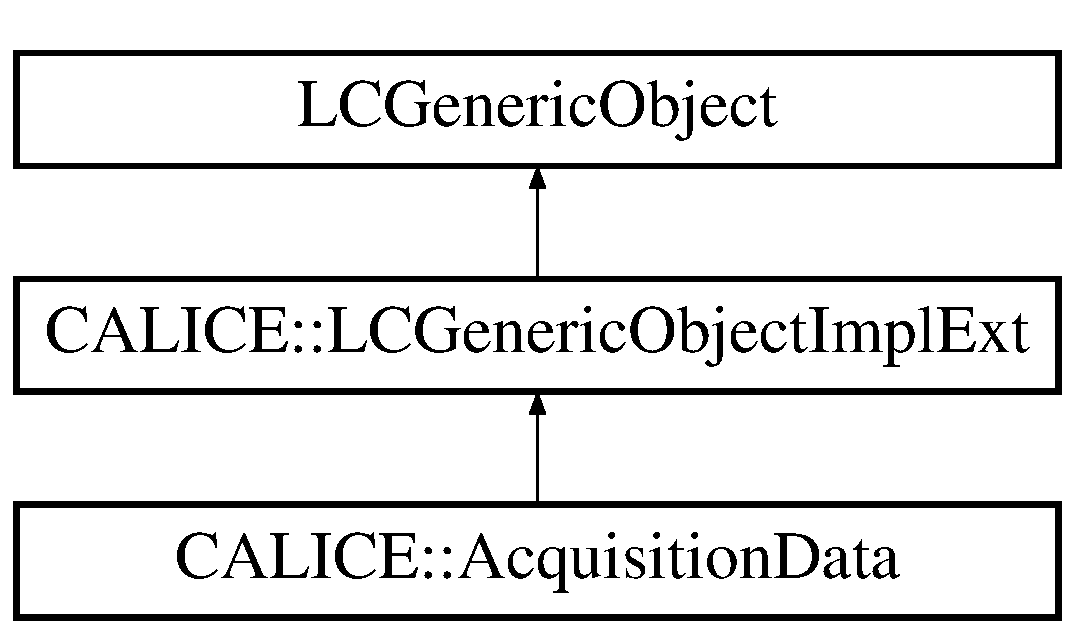
\includegraphics[height=3.000000cm]{classCALICE_1_1AcquisitionData}
\end{center}
\end{figure}
\subsection*{Public Member Functions}
\begin{DoxyCompactItemize}
\item 
{\bf Acquisition\-Data} (int acquisition\-Number\-In\-Run, int acquisition\-Number\-In\-Configuration)\label{classCALICE_1_1AcquisitionData_aa1f1d0bd5bbb808113b480b760b357ef}

\begin{DoxyCompactList}\small\item\em The constructor. \end{DoxyCompactList}\item 
{\bf Acquisition\-Data} (L\-C\-Object $\ast${\bf obj})\label{classCALICE_1_1AcquisitionData_a80ddf44bcb6c9070a4774aa640072c46}

\begin{DoxyCompactList}\small\item\em A copy constructor. \end{DoxyCompactList}\item 
virtual {\bf $\sim$\-Acquisition\-Data} ()\label{classCALICE_1_1AcquisitionData_a03dba78272df176732377006a3e6415c}

\begin{DoxyCompactList}\small\item\em The destructor. \end{DoxyCompactList}\item 
{\bf Acquisition\-Data} \& {\bf set\-Acquisition\-State} (bool acqstate)\label{classCALICE_1_1AcquisitionData_a3f6cf1b411af4a4c73822f3843ce5f9d}

\begin{DoxyCompactList}\small\item\em Sets the acquisition state, start=1, end=0. \end{DoxyCompactList}\item 
bool {\bf get\-Acquisition\-State} () const \label{classCALICE_1_1AcquisitionData_afb3d781c28f16db8508bf837864aca54}

\begin{DoxyCompactList}\small\item\em Returns the acquisition state. \end{DoxyCompactList}\item 
{\bf Acquisition\-Data} \& {\bf set\-Time\-Information\-Sec} (unsigned int timeinfo)
\begin{DoxyCompactList}\small\item\em Set the time information for the given state (in sec), note that the meaning is different for start and end. \end{DoxyCompactList}\item 
{\bf Acquisition\-Data} \& {\bf set\-Time\-Information\-Mu\-Sec} (unsigned int timeinfo)
\begin{DoxyCompactList}\small\item\em Set the time information for the given state (in sec), note that the meaning is different for start and end. \end{DoxyCompactList}\item 
unsigned int {\bf get\-Acquisition\-Number\-In\-Run} ()\label{classCALICE_1_1AcquisitionData_a30dc6e6cf5801240dc672e73703de4f3}

\begin{DoxyCompactList}\small\item\em returns the acquisition number in run \end{DoxyCompactList}\item 
unsigned int {\bf get\-Acquisition\-Number\-In\-Configuration} ()\label{classCALICE_1_1AcquisitionData_a5fdfe4f39cf7c10682eab629243a35f6}

\begin{DoxyCompactList}\small\item\em returns the acquisition number in configuration \end{DoxyCompactList}\item 
{\bf Acquisition\-Data} \& {\bf set\-Event\-Number\-Info} (unsigned int evnuminfo)\label{classCALICE_1_1AcquisitionData_a3bab96bafcf9d8badea581d70a9a1778}

\begin{DoxyCompactList}\small\item\em Sets the eventnumber info. \end{DoxyCompactList}\item 
unsigned int {\bf get\-Max\-Event\-Number\-In\-Acquisition} ()\label{classCALICE_1_1AcquisitionData_a4bb9e5f8e2e5e7be1705557db6ff579e}

\begin{DoxyCompactList}\small\item\em returns the maximal number of events in Acquisition \end{DoxyCompactList}\item 
unsigned int {\bf get\-Act\-Event\-Number\-In\-Acquisition} ()\label{classCALICE_1_1AcquisitionData_a0a3fa8fe5a5a06930597e9b8a3aeb92c}

\begin{DoxyCompactList}\small\item\em returns the actual number of events in Acquisition \end{DoxyCompactList}\item 
unsigned int {\bf get\-Max\-Acquisition\-Time\-Sec} ()\label{classCALICE_1_1AcquisitionData_ac3b5becc7288c4cf71b99e9f81c9a564}

\begin{DoxyCompactList}\small\item\em Returns the maximum acquisition time -\/ seconds. \end{DoxyCompactList}\item 
unsigned int {\bf get\-Max\-Acquisition\-Time\-Mus} ()\label{classCALICE_1_1AcquisitionData_ab076903057bb3f4a85a144661a3d4223}

\begin{DoxyCompactList}\small\item\em Returns the maximum acquisition time -\/ microseconds. \end{DoxyCompactList}\item 
unsigned int {\bf get\-Act\-Acquisition\-Time\-Sec} ()\label{classCALICE_1_1AcquisitionData_a9c32aed54c8525c4dd143594ebf572e6}

\begin{DoxyCompactList}\small\item\em Returns the actual acquisition time -\/ seconds. \end{DoxyCompactList}\item 
unsigned int {\bf get\-Act\-Acquisition\-Time\-Mus} ()\label{classCALICE_1_1AcquisitionData_a31cc8badfb06afa9ca37db0af726cd27}

\begin{DoxyCompactList}\small\item\em Returns the actual acquisition time -\/ microseconds. \end{DoxyCompactList}\item 
{\bf Acquisition\-Data} \& {\bf set\-Dif\-Info\-Present} (bool difdatapresent)\label{classCALICE_1_1AcquisitionData_a708b7f09773470d122d82594b2aaf743}

\begin{DoxyCompactList}\small\item\em Set whether there are dif data in the acquisition. \end{DoxyCompactList}\item 
bool {\bf get\-Dif\-Data\-Present} () const \label{classCALICE_1_1AcquisitionData_a2f75303f2065483675cc11b596d66fdb}

\begin{DoxyCompactList}\small\item\em Return whether dif data are present in the acquisition. \end{DoxyCompactList}\item 
{\bf Acquisition\-Data} \& {\bf set\-Dif\-Trigger\-Counter} (unsigned int triggercounter)\label{classCALICE_1_1AcquisitionData_a47d04ea74eb9197cb24353b1c3a5d9ea}

\begin{DoxyCompactList}\small\item\em Check dif trigger counter at acquisition start and end. \end{DoxyCompactList}\item 
unsigned int {\bf get\-Dif\-Trigger\-Counter} () const \label{classCALICE_1_1AcquisitionData_a5901280a12cf53272af6ea1a903a5616}

\begin{DoxyCompactList}\small\item\em Return dif trigger counter. \end{DoxyCompactList}\item 
{\bf Acquisition\-Data} \& {\bf set\-Numberof\-Dif\-Buffer\-Words} (unsigned int difbufferwords)\label{classCALICE_1_1AcquisitionData_a1a64594b02fe07d2f8c985481a9aedac}

\begin{DoxyCompactList}\small\item\em Check number of dif buffer words. \end{DoxyCompactList}\item 
unsigned int {\bf get\-Numberof\-Dif\-Buffer\-Words} ()\label{classCALICE_1_1AcquisitionData_a54292d25b63278bcf9d1f62daf623c8e}

\begin{DoxyCompactList}\small\item\em Return number of dif trigger buffer words. \end{DoxyCompactList}\item 
const std\-::string {\bf get\-Type\-Name} () const \label{classCALICE_1_1AcquisitionData_af5b75abdb744f5511107bf592abd7564}

\begin{DoxyCompactList}\small\item\em returns the the type name \end{DoxyCompactList}\item 
const std\-::string {\bf get\-Data\-Description} () const \label{classCALICE_1_1AcquisitionData_aaa8b0ef98afc2ebc20bd111802ad96a2}

\begin{DoxyCompactList}\small\item\em returns a brief description of the data stored \end{DoxyCompactList}\item 
std\-::ostream \& {\bf print} (std\-::ostream \&ostrm)\label{classCALICE_1_1AcquisitionData_aaa13de3cfac3a3f6a4babccb767d7cd9}

\begin{DoxyCompactList}\small\item\em dumps data content \end{DoxyCompactList}\end{DoxyCompactItemize}
\subsection*{Additional Inherited Members}


\subsection{Detailed Description}
Class to store acquisition data info, i.\-e. 

acquisiton\# in run, acquisition\# in configuration,max. events in acquistion

Note this is for internal use only \begin{DoxyRefDesc}{Todo}
\item[{\bf Todo}]should we make a regular userlib class out of it? \end{DoxyRefDesc}
\begin{DoxyAuthor}{Author}
R. P�schl (L\-A\-L Orsay) 
\end{DoxyAuthor}
\begin{DoxyDate}{Date}
Feb 27 2006 
\end{DoxyDate}


Definition at line 44 of file Acquisition\-Data.\-hh.



\subsection{Member Function Documentation}
\index{C\-A\-L\-I\-C\-E\-::\-Acquisition\-Data@{C\-A\-L\-I\-C\-E\-::\-Acquisition\-Data}!set\-Time\-Information\-Mu\-Sec@{set\-Time\-Information\-Mu\-Sec}}
\index{set\-Time\-Information\-Mu\-Sec@{set\-Time\-Information\-Mu\-Sec}!CALICE::AcquisitionData@{C\-A\-L\-I\-C\-E\-::\-Acquisition\-Data}}
\subsubsection[{set\-Time\-Information\-Mu\-Sec}]{\setlength{\rightskip}{0pt plus 5cm}{\bf Acquisition\-Data}\& C\-A\-L\-I\-C\-E\-::\-Acquisition\-Data\-::set\-Time\-Information\-Mu\-Sec (
\begin{DoxyParamCaption}
\item[{unsigned int}]{timeinfo}
\end{DoxyParamCaption}
)\hspace{0.3cm}{\ttfamily [inline]}}\label{classCALICE_1_1AcquisitionData_a0c06ac70f5934b81cc241b447201b881}


Set the time information for the given state (in sec), note that the meaning is different for start and end. 

This will be handled further down 

Definition at line 104 of file Acquisition\-Data.\-hh.

\index{C\-A\-L\-I\-C\-E\-::\-Acquisition\-Data@{C\-A\-L\-I\-C\-E\-::\-Acquisition\-Data}!set\-Time\-Information\-Sec@{set\-Time\-Information\-Sec}}
\index{set\-Time\-Information\-Sec@{set\-Time\-Information\-Sec}!CALICE::AcquisitionData@{C\-A\-L\-I\-C\-E\-::\-Acquisition\-Data}}
\subsubsection[{set\-Time\-Information\-Sec}]{\setlength{\rightskip}{0pt plus 5cm}{\bf Acquisition\-Data}\& C\-A\-L\-I\-C\-E\-::\-Acquisition\-Data\-::set\-Time\-Information\-Sec (
\begin{DoxyParamCaption}
\item[{unsigned int}]{timeinfo}
\end{DoxyParamCaption}
)\hspace{0.3cm}{\ttfamily [inline]}}\label{classCALICE_1_1AcquisitionData_a42d0b8ad6f9ba2bfddb3af8b2683dfa5}


Set the time information for the given state (in sec), note that the meaning is different for start and end. 

This will be handled further down 

Definition at line 97 of file Acquisition\-Data.\-hh.



The documentation for this class was generated from the following files\-:\begin{DoxyCompactItemize}
\item 
Acquisition\-Data.\-hh\item 
Acquisition\-Data.\-cc\end{DoxyCompactItemize}

\section{C\-A\-L\-I\-C\-E\-:\-:Adc\-Block Class Reference}
\label{classCALICE_1_1AdcBlock}\index{C\-A\-L\-I\-C\-E\-::\-Adc\-Block@{C\-A\-L\-I\-C\-E\-::\-Adc\-Block}}


Class for the A\-D\-C Data as acquired by the \doxyref{C\-A\-L\-I\-C\-E}{p.}{namespaceCALICE} D\-A\-Q.  




{\ttfamily \#include $<$Adc\-Block.\-hh$>$}

Inheritance diagram for C\-A\-L\-I\-C\-E\-:\-:Adc\-Block\-:\begin{figure}[H]
\begin{center}
\leavevmode
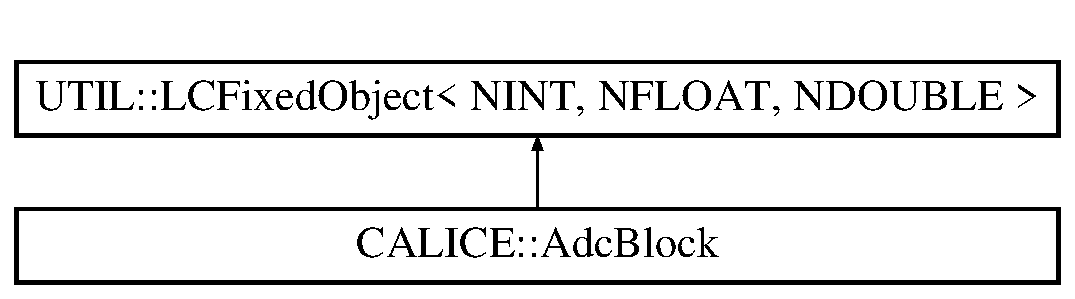
\includegraphics[height=2.000000cm]{classCALICE_1_1AdcBlock}
\end{center}
\end{figure}
\subsection*{Public Member Functions}
\begin{DoxyCompactItemize}
\item 
{\bf Adc\-Block} (int board\-I\-D, int label, int Fe, int Imul, const Adc\-Block\-Array \&adc\-Block, int status)\label{classCALICE_1_1AdcBlock_a6cfc92f7005861497f3da19929b3305c}

\begin{DoxyCompactList}\small\item\em Convenient c'tor. \end{DoxyCompactList}\item 
{\bf Adc\-Block} (L\-C\-Object $\ast$obj)\label{classCALICE_1_1AdcBlock_ab78d098d531e821e759f4f82db0942de}

\begin{DoxyCompactList}\small\item\em 'Copy constructor' needed to interpret L\-C\-Collection read from file/database. \end{DoxyCompactList}\item 
virtual {\bf $\sim$\-Adc\-Block} ()\label{classCALICE_1_1AdcBlock_af3dc2bf5b9ef534971a256f5b15d51dd}

\begin{DoxyCompactList}\small\item\em Important for memory handling. \end{DoxyCompactList}\item 
unsigned int {\bf get\-Board\-I\-D} () const \label{classCALICE_1_1AdcBlock_a9a8352cd4be0a403b477ac602217ca3a}

\begin{DoxyCompactList}\small\item\em get the board id. \end{DoxyCompactList}\item 
unsigned {\bf get\-Elec\-Channel} (int) const 
\begin{DoxyCompactList}\small\item\em the class interface\-: \end{DoxyCompactList}\item 
short {\bf get\-Adc\-Val} (int i) const \label{classCALICE_1_1AdcBlock_a3c78cb752efdb526d69c64f17c880616}

\begin{DoxyCompactList}\small\item\em and the actual A\-D\-C calue \end{DoxyCompactList}\item 
short {\bf get\-Board\-Front\-End} () const \label{classCALICE_1_1AdcBlock_aeba50c8fb0cb56a399027c1a24254d96}

\begin{DoxyCompactList}\small\item\em Information on the F\-E chip the data was received. \end{DoxyCompactList}\item 
short {\bf get\-Multiplex\-Position} () const \label{classCALICE_1_1AdcBlock_a2978073ea8348f69e62bb0cbe15cab10}

\begin{DoxyCompactList}\small\item\em and the position within the series of transmissions \end{DoxyCompactList}\item 
short {\bf get\-Crate\-I\-D} () const \label{classCALICE_1_1AdcBlock_a6bcccdc816b7c0cf695a7853071ffe6f}

\begin{DoxyCompactList}\small\item\em Some general information on the board on which the data was received on the Crate Id. \end{DoxyCompactList}\item 
short {\bf get\-Slot\-I\-D} () const \label{classCALICE_1_1AdcBlock_a13560d4d9931ac08b13052580f67969a}

\begin{DoxyCompactList}\small\item\em on the Slot Id \end{DoxyCompactList}\item 
short {\bf get\-Board\-Component\-Number} () const \label{classCALICE_1_1AdcBlock_ab782b69f80d4226d89a8b98221935c1b}

\begin{DoxyCompactList}\small\item\em on the Board\-Component Number \end{DoxyCompactList}\item 
short {\bf get\-Record\-Label} () const \label{classCALICE_1_1AdcBlock_af22b4a1cedb615b08899904eed3725bc}

\begin{DoxyCompactList}\small\item\em on the Board Label \end{DoxyCompactList}\item 
short {\bf get\-Transmission\-Status} () const \label{classCALICE_1_1AdcBlock_a8e9c8c2fe91eeed4f202aee8497c1854}

\begin{DoxyCompactList}\small\item\em Transmission of data from piggy back to F\-E. \end{DoxyCompactList}\item 
void {\bf print} (std\-::ostream \&os, int)\label{classCALICE_1_1AdcBlock_a6bd9f304b2fada336341073e07c41f13}

\begin{DoxyCompactList}\small\item\em Convenient print method. \end{DoxyCompactList}\item 
const std\-::string {\bf get\-Type\-Name} () const \label{classCALICE_1_1AdcBlock_aeba86a15ac0ad04d3564bae5aec911fb}

\begin{DoxyCompactList}\small\item\em Return the type of the class. \end{DoxyCompactList}\item 
const std\-::string {\bf get\-Data\-Description} () const \label{classCALICE_1_1AdcBlock_a0f2e508485b4214ab454b72fc0c591ed}

\begin{DoxyCompactList}\small\item\em Return a brief description of the data members. \end{DoxyCompactList}\end{DoxyCompactItemize}


\subsection{Detailed Description}
Class for the A\-D\-C Data as acquired by the \doxyref{C\-A\-L\-I\-C\-E}{p.}{namespaceCALICE} D\-A\-Q. 

The class reflects that the data are received in chunks of 12 A\-D\-C's within a series of 18 transmissions (multiplexing).

A\-D\-C data are stored together with the indices of the board by which they were received, the F\-E (0-\/8) and their position within the multiplexed series (0-\/17). The class provides interface functions to get the adc value within the adc block as well as an associated electronic channel id\-: Elec\-Channel\-I\-D = Crate\-I\-D , Slot\-I\-D, F\-E, Multipl., A\-D\-C\-\_\-i\-: Bit\-: 31-\/24 , 23-\/16, 15-\/12, 11-\/4 , 3-\/0 \begin{DoxyAuthor}{Author}
R. P�schl D\-E\-S\-Y 
\end{DoxyAuthor}
\begin{DoxyDate}{Date}
Mar 5 2005 
\end{DoxyDate}


Definition at line 34 of file Adc\-Block.\-hh.



\subsection{Member Function Documentation}
\index{C\-A\-L\-I\-C\-E\-::\-Adc\-Block@{C\-A\-L\-I\-C\-E\-::\-Adc\-Block}!get\-Elec\-Channel@{get\-Elec\-Channel}}
\index{get\-Elec\-Channel@{get\-Elec\-Channel}!CALICE::AdcBlock@{C\-A\-L\-I\-C\-E\-::\-Adc\-Block}}
\subsubsection[{get\-Elec\-Channel}]{\setlength{\rightskip}{0pt plus 5cm}unsigned C\-A\-L\-I\-C\-E\-::\-Adc\-Block\-::get\-Elec\-Channel (
\begin{DoxyParamCaption}
\item[{int}]{i}
\end{DoxyParamCaption}
) const}\label{classCALICE_1_1AdcBlock_af03eee5e03977fbab76d5fc98d113ef8}


the class interface\-: 

get electronic channel id assigned to the adc 

Definition at line 9 of file Adc\-Block.\-cc.



The documentation for this class was generated from the following files\-:\begin{DoxyCompactItemize}
\item 
Adc\-Block.\-hh\item 
Adc\-Block.\-cc\end{DoxyCompactItemize}

\section{C\-A\-L\-I\-C\-E\-:\-:Ahc2\-Calibrations Class Reference}
\label{classCALICE_1_1Ahc2Calibrations}\index{C\-A\-L\-I\-C\-E\-::\-Ahc2\-Calibrations@{C\-A\-L\-I\-C\-E\-::\-Ahc2\-Calibrations}}


storing all informations necessary to calibrate a H\-B\-U Si\-P\-M read channel  




{\ttfamily \#include $<$Ahc2\-Calibrations.\-hh$>$}

\subsection*{Public Member Functions}
\begin{DoxyCompactItemize}
\item 
{\bfseries Ahc2\-Calibrations} ({\bf Linear\-Fit\-Compound} $\ast$M\-I\-P, {\bf Linear\-Fit\-Compound} $\ast$gain, {\bf Simple\-Value} $\ast$pedestal, {\bf Simple\-Value\-Vector} $\ast$pedestal\-Memory\-Cell\-Offset, {\bf Simple\-Value} $\ast$low\-Gain\-Pedestal, {\bf Simple\-Value\-Vector} $\ast$low\-Gain\-Pedestal\-Memory\-Cell\-Offset, {\bf Simple\-Value} $\ast$inter\-Calibration, {\bf Simple\-Value} $\ast$inter\-Calibration\-Physics\-Calib, {\bf Simple\-Value} $\ast$temperature, {\bf Saturation\-Parameters} $\ast$saturation, {\bf Simple\-Value\-Vector} $\ast$time\-Slopes\-Calibration, {\bf Simple\-Value\-Vector} $\ast$time\-Offset\-Calibration, {\bf Simple\-Value\-Vector} $\ast$time\-Offset\-Mem\-Cell\-Even\-Calibration, {\bf Simple\-Value\-Vector} $\ast$time\-Offset\-Mem\-Cell\-Odd\-Calibration, {\bf Simple\-Value\-Vector} $\ast$time\-Offset\-Mem\-Cell\-Even\-Buffer\-Even\-Event\-Even\-Calibration, {\bf Simple\-Value\-Vector} $\ast$time\-Offset\-Mem\-Cell\-Odd\-Buffer\-Even\-Event\-Odd\-Calibration, {\bf Simple\-Value\-Vector} $\ast$time\-Offset\-Mem\-Cell\-Even\-Buffer\-Odd\-Event\-Even\-Calibration, {\bf Simple\-Value\-Vector} $\ast$time\-Offset\-Mem\-Cell\-Odd\-Buffer\-Odd\-Event\-Odd\-Calibration, {\bf Simple\-Value\-Vector} $\ast$Occupancy\-Bxid\-Even\-High\-Gain\-Calibration, {\bf Simple\-Value\-Vector} $\ast$Occupancy\-Bxid\-Even\-Low\-Gain\-Calibration, {\bf Simple\-Value\-Vector} $\ast$Occupancy\-Bxid\-Odd\-High\-Gain\-Calibration, {\bf Simple\-Value\-Vector} $\ast$Occupancy\-Bxid\-Odd\-Low\-Gain\-Calibration, const int status, const int cell\-I\-D, const std\-::string \&cell\-I\-D\-Encoding)\label{classCALICE_1_1Ahc2Calibrations_a9888f56fc5fc4a2527d8b69560a017a0}

\item 
{\bf Linear\-Fit\-Compound} $\ast$ {\bfseries get\-M\-I\-P} () const \label{classCALICE_1_1Ahc2Calibrations_a8fdd3c513f5bb8ff484ece6173dbf3fe}

\item 
{\bf Linear\-Fit\-Compound} $\ast$ {\bfseries get\-Gain} () const \label{classCALICE_1_1Ahc2Calibrations_ab4a252f2e7589fd8429a65774181ecb3}

\item 
{\bf Simple\-Value} $\ast$ {\bfseries get\-Pedestal} () const \label{classCALICE_1_1Ahc2Calibrations_ae1c09b266458a55af0f854cbd714231c}

\item 
{\bf Simple\-Value\-Vector} $\ast$ {\bfseries get\-Pedestal\-Memory\-Cell\-Offset} () const \label{classCALICE_1_1Ahc2Calibrations_a07a161f7ea41cdea8a91af0e56740381}

\item 
{\bf Simple\-Value} $\ast$ {\bfseries get\-Low\-Gain\-Pedestal} () const \label{classCALICE_1_1Ahc2Calibrations_a63bd021a647dbdac00f22e387fdf522a}

\item 
{\bf Simple\-Value\-Vector} $\ast$ {\bfseries get\-Low\-Gain\-Pedestal\-Memory\-Cell\-Offset} () const \label{classCALICE_1_1Ahc2Calibrations_a89f9629d85227f1a04e6241a2953487c}

\item 
{\bf Simple\-Value} $\ast$ {\bfseries get\-Inter\-Calibration} () const \label{classCALICE_1_1Ahc2Calibrations_a8edc2b5e2d253116996be42c6c7cd90c}

\item 
{\bf Simple\-Value} $\ast$ {\bfseries get\-Physics\-Calib\-I\-C} () const \label{classCALICE_1_1Ahc2Calibrations_abc1a937aac4a27234ac474901a847624}

\item 
{\bf Simple\-Value} $\ast$ {\bfseries get\-Temperature} () const \label{classCALICE_1_1Ahc2Calibrations_a0169760750c84e6341f5293e8347cf75}

\item 
{\bf Saturation\-Parameters} $\ast$ {\bfseries get\-Saturation} () const \label{classCALICE_1_1Ahc2Calibrations_acfbbab2fcfc1353175bf2196512122a5}

\item 
{\bf Simple\-Value\-Vector} $\ast$ {\bfseries get\-Time\-Slopes} () const \label{classCALICE_1_1Ahc2Calibrations_a2d565ca0cdc228535d932845c2e25bc5}

\item 
{\bf Simple\-Value\-Vector} $\ast$ {\bfseries get\-Time\-Offset} () const \label{classCALICE_1_1Ahc2Calibrations_a2ea94518b27fc02638ff22330ee8d22b}

\item 
{\bf Simple\-Value\-Vector} $\ast$ {\bfseries get\-Time\-Offset\-Mem\-Cell\-Even} () const \label{classCALICE_1_1Ahc2Calibrations_a63e61adf723ae249438dcbf9cfb826c9}

\item 
{\bf Simple\-Value\-Vector} $\ast$ {\bfseries get\-Time\-Offset\-Mem\-Cell\-Odd} () const \label{classCALICE_1_1Ahc2Calibrations_a8cba3c625997c6c9748216e0c3237581}

\item 
{\bf Simple\-Value\-Vector} $\ast$ {\bfseries get\-Time\-Offset\-Mem\-Cell\-Even\-Buffer\-Even\-Event\-Even} () const \label{classCALICE_1_1Ahc2Calibrations_a06cc210cba3b0b64c5246b2afc3bfb12}

\item 
{\bf Simple\-Value\-Vector} $\ast$ {\bfseries get\-Time\-Offset\-Mem\-Cell\-Odd\-Buffer\-Even\-Event\-Odd} () const \label{classCALICE_1_1Ahc2Calibrations_a1c0284bbce4bddd84e29a66db9d5a5f5}

\item 
{\bf Simple\-Value\-Vector} $\ast$ {\bfseries get\-Time\-Offset\-Mem\-Cell\-Even\-Buffer\-Odd\-Event\-Even} () const \label{classCALICE_1_1Ahc2Calibrations_af43febbfc161a9ee021fb9a63fd825cc}

\item 
{\bf Simple\-Value\-Vector} $\ast$ {\bfseries get\-Time\-Offset\-Mem\-Cell\-Odd\-Buffer\-Odd\-Event\-Odd} () const \label{classCALICE_1_1Ahc2Calibrations_a158d4b34cc236a5e1470d5845ebb8dd6}

\item 
{\bf Simple\-Value\-Vector} $\ast$ {\bfseries get\-Occupancy\-Bxid\-Even\-High\-Gain} () const \label{classCALICE_1_1Ahc2Calibrations_ac146a72bf6f6cf3b35a4f01799f97c86}

\item 
{\bf Simple\-Value\-Vector} $\ast$ {\bfseries get\-Occupancy\-Bxid\-Even\-Low\-Gain} () const \label{classCALICE_1_1Ahc2Calibrations_ac5e9fc14adce26175532a3997f3368d9}

\item 
{\bf Simple\-Value\-Vector} $\ast$ {\bfseries get\-Occupancy\-Bxid\-Odd\-High\-Gain} () const \label{classCALICE_1_1Ahc2Calibrations_a5042f6033737a0d31308346080b744d7}

\item 
{\bf Simple\-Value\-Vector} $\ast$ {\bfseries get\-Occupancy\-Bxid\-Odd\-Low\-Gain} () const \label{classCALICE_1_1Ahc2Calibrations_a6c7c82893d57b4baa455d88fe74e93dc}

\item 
int {\bfseries get\-Status} () const \label{classCALICE_1_1Ahc2Calibrations_abd138930b5b67cda32960a1e5805369f}

\item 
int {\bfseries get\-Cell\-I\-D} () const \label{classCALICE_1_1Ahc2Calibrations_a863df224a883b4075531d5718a309959}

\item 
const std\-::string \& {\bfseries get\-Cell\-I\-D\-Encoding} () const \label{classCALICE_1_1Ahc2Calibrations_a912aefba37f34f874a3c05ae029d9f10}

\item 
void {\bfseries set\-M\-I\-P} ({\bf Linear\-Fit\-Compound} $\ast$M\-I\-P)\label{classCALICE_1_1Ahc2Calibrations_a579397bf370b64b210647a449fece2cb}

\item 
void {\bfseries set\-Gain} ({\bf Linear\-Fit\-Compound} $\ast$gain)\label{classCALICE_1_1Ahc2Calibrations_ab6cad8fd192851c21edbbd6aa1814f68}

\item 
void {\bfseries set\-Pedestal} ({\bf Simple\-Value} $\ast$pedestal)\label{classCALICE_1_1Ahc2Calibrations_a8b2e58c97f7e5b5a25fd07d66333d95d}

\item 
void {\bfseries set\-Pedestal\-Memory\-Cell\-Offset} ({\bf Simple\-Value\-Vector} $\ast$pedestal\-Memory\-Cell\-Offset)\label{classCALICE_1_1Ahc2Calibrations_a40e89ab42152fb10a2b4318d6b6d2588}

\item 
void {\bfseries set\-Low\-Gain\-Pedestal} ({\bf Simple\-Value} $\ast$low\-Gain\-Pedestal)\label{classCALICE_1_1Ahc2Calibrations_a555a2738d250d0c98c3b263dada3ca8d}

\item 
void {\bfseries set\-Low\-Gain\-Pedestal\-Memory\-Cell\-Offset} ({\bf Simple\-Value\-Vector} $\ast$low\-Gain\-Pedestal\-Memory\-Cell\-Offset)\label{classCALICE_1_1Ahc2Calibrations_ae8f9e0eb9e2209a8cb608a0edac16c78}

\item 
void {\bfseries set\-Inter\-Calibration} ({\bf Simple\-Value} $\ast$inter\-Calibration)\label{classCALICE_1_1Ahc2Calibrations_a7a5db8ef5f4c3f2aab84889b54c15852}

\item 
void {\bfseries set\-Physics\-Calib\-I\-C} ({\bf Simple\-Value} $\ast$inter\-Calibration\-Physics\-Calib)\label{classCALICE_1_1Ahc2Calibrations_ac83d32c7dac04831bd8890c357e2e49c}

\item 
void {\bfseries set\-Temperature} ({\bf Simple\-Value} $\ast$temperature)\label{classCALICE_1_1Ahc2Calibrations_ae1409d9eb74bc38bbce60f13231df61d}

\item 
void {\bfseries set\-Saturation} ({\bf Saturation\-Parameters} $\ast$param)\label{classCALICE_1_1Ahc2Calibrations_acd5284f9adbcd950fe3caa9244495a34}

\item 
void {\bfseries set\-Time\-Slopes} ({\bf Simple\-Value\-Vector} $\ast$time\-Slopes)\label{classCALICE_1_1Ahc2Calibrations_a673f9d436e10789805e539773b5a4887}

\item 
void {\bfseries set\-Time\-Offset} ({\bf Simple\-Value\-Vector} $\ast$time\-Offset)\label{classCALICE_1_1Ahc2Calibrations_a1f7aa8d3c84e57b7474a40be2ad1ee30}

\item 
void {\bfseries set\-Time\-Offset\-Mem\-Cell\-Even} ({\bf Simple\-Value\-Vector} $\ast$time\-Offset\-Mem\-Cell\-Even)\label{classCALICE_1_1Ahc2Calibrations_a9b04c99d86154e79c216d3c7d3406536}

\item 
void {\bfseries set\-Time\-Offset\-Mem\-Cell\-Odd} ({\bf Simple\-Value\-Vector} $\ast$time\-Offset\-Mem\-Cell\-Odd)\label{classCALICE_1_1Ahc2Calibrations_a431ae56f79d026c1f8f5d409c2abea72}

\item 
void {\bfseries set\-Time\-Offset\-Mem\-Cell\-Even\-Buffer\-Even\-Event\-Even} ({\bf Simple\-Value\-Vector} $\ast$time\-Offset\-Mem\-Cell\-Even\-Buffer\-Even\-Event\-Even)\label{classCALICE_1_1Ahc2Calibrations_a83670559cf0efbfaee9c16de5da5c0a6}

\item 
void {\bfseries set\-Time\-Offset\-Mem\-Cell\-Odd\-Buffer\-Even\-Event\-Odd} ({\bf Simple\-Value\-Vector} $\ast$time\-Offset\-Mem\-Cell\-Odd\-Buffer\-Even\-Event\-Odd)\label{classCALICE_1_1Ahc2Calibrations_af841493f85e968bf6048c1ac5198a668}

\item 
void {\bfseries set\-Time\-Offset\-Mem\-Cell\-Even\-Buffer\-Odd\-Event\-Even} ({\bf Simple\-Value\-Vector} $\ast$time\-Offset\-Mem\-Cell\-Even\-Buffer\-Odd\-Event\-Even)\label{classCALICE_1_1Ahc2Calibrations_a5c5ceb502f5d2eb42461665297c9e48e}

\item 
void {\bfseries set\-Time\-Offset\-Mem\-Cell\-Odd\-Buffer\-Odd\-Event\-Odd} ({\bf Simple\-Value\-Vector} $\ast$time\-Offset\-Mem\-Cell\-Odd\-Buffer\-Odd\-Event\-Odd)\label{classCALICE_1_1Ahc2Calibrations_ad5e1ecb7f3038ea9219e3df6e076a289}

\item 
void {\bfseries set\-Occupancy\-Bxid\-Even\-High\-Gain} ({\bf Simple\-Value\-Vector} $\ast$Occupancy\-Bxid\-Even\-High\-Gain)\label{classCALICE_1_1Ahc2Calibrations_a0c47dbd7e02f41eb37807708b69b6d96}

\item 
void {\bfseries set\-Occupancy\-Bxid\-Even\-Low\-Gain} ({\bf Simple\-Value\-Vector} $\ast$Occupancy\-Bxid\-Even\-Low\-Gain)\label{classCALICE_1_1Ahc2Calibrations_ac9ea2f871722475812b3045cf6272330}

\item 
void {\bfseries set\-Occupancy\-Bxid\-Odd\-High\-Gain} ({\bf Simple\-Value\-Vector} $\ast$Occupancy\-Bxid\-Odd\-High\-Gain)\label{classCALICE_1_1Ahc2Calibrations_a6f5df40413007ffdc43bc76c34b21e20}

\item 
void {\bfseries set\-Occupancy\-Bxid\-Odd\-Low\-Gain} ({\bf Simple\-Value\-Vector} $\ast$Occupancy\-Bxid\-Odd\-Low\-Gain)\label{classCALICE_1_1Ahc2Calibrations_a9e0edbae2eed1dec6cc9c13581c7297c}

\item 
void {\bfseries set\-Status} (const int status)\label{classCALICE_1_1Ahc2Calibrations_ad5435a2ccdfa548e16c8c7a6dbdacb77}

\item 
void {\bfseries set\-Cell\-I\-D} (const int cell\-I\-D)\label{classCALICE_1_1Ahc2Calibrations_a34bbc74589d8a3e41719c5ce3cff3a38}

\item 
void {\bfseries set\-Cell\-I\-D\-Encoding} (const std\-::string \&encoding)\label{classCALICE_1_1Ahc2Calibrations_a09ce017f8db987840a98331781425d68}

\end{DoxyCompactItemize}
\subsection*{Private Attributes}
\begin{DoxyCompactItemize}
\item 
{\bf Linear\-Fit\-Compound} $\ast$ {\bfseries \-\_\-gain}\label{classCALICE_1_1Ahc2Calibrations_a03eefbf76823ac538ac161116c721094}

\item 
{\bf Linear\-Fit\-Compound} $\ast$ {\bfseries \-\_\-\-M\-I\-P}\label{classCALICE_1_1Ahc2Calibrations_a62f955858c113f4d74839b775431573f}

\item 
{\bf Simple\-Value} $\ast$ {\bfseries \-\_\-pedestal}\label{classCALICE_1_1Ahc2Calibrations_a4efe9ef32165ddb8b060e1cea599662c}

\item 
{\bf Simple\-Value\-Vector} $\ast$ {\bfseries \-\_\-pedestal\-Memory\-Cell\-Offset}\label{classCALICE_1_1Ahc2Calibrations_ad99c21640b4a8c7a5cfd4eef39d71888}

\item 
{\bf Simple\-Value} $\ast$ {\bfseries \-\_\-low\-Gain\-Pedestal}\label{classCALICE_1_1Ahc2Calibrations_a6738b35d654551de7e2da86c3bf28160}

\item 
{\bf Simple\-Value\-Vector} $\ast$ {\bfseries \-\_\-low\-Gain\-Pedestal\-Memory\-Cell\-Offset}\label{classCALICE_1_1Ahc2Calibrations_a588aba128c20afe6769157d9e14cc674}

\item 
{\bf Simple\-Value} $\ast$ {\bfseries \-\_\-inter\-Calibration}\label{classCALICE_1_1Ahc2Calibrations_ae4efcf3a0b9a4f68a0b0bec543f1127f}

\item 
{\bf Simple\-Value} $\ast$ {\bfseries \-\_\-inter\-Calibration\-Physics\-Calib}\label{classCALICE_1_1Ahc2Calibrations_a857c20a5260ad72e67fd331b714e95e5}

\item 
{\bf Simple\-Value} $\ast$ {\bfseries \-\_\-temperature}\label{classCALICE_1_1Ahc2Calibrations_aa3af368bb355aedaa207832852ebf38a}

\item 
{\bf Saturation\-Parameters} $\ast$ {\bfseries \-\_\-saturation}\label{classCALICE_1_1Ahc2Calibrations_af91d92efebefb744991268c919b2f8c6}

\item 
{\bf Simple\-Value\-Vector} $\ast$ {\bfseries \-\_\-time\-Slopes\-Calibration}\label{classCALICE_1_1Ahc2Calibrations_a07e277795a54bda83dd8b3d866b7bdf7}

\item 
{\bf Simple\-Value\-Vector} $\ast$ {\bfseries \-\_\-time\-Offset\-Calibration}\label{classCALICE_1_1Ahc2Calibrations_ab69dc6a5c19ed04cf5fd2f662db49f4d}

\item 
{\bf Simple\-Value\-Vector} $\ast$ {\bfseries \-\_\-time\-Offset\-Mem\-Cell\-Even\-Calibration}\label{classCALICE_1_1Ahc2Calibrations_aed33bff61e370b8720cbca5d2f218b59}

\item 
{\bf Simple\-Value\-Vector} $\ast$ {\bfseries \-\_\-time\-Offset\-Mem\-Cell\-Odd\-Calibration}\label{classCALICE_1_1Ahc2Calibrations_aca2f68025de9861d3e7cc8272b03aaf9}

\item 
{\bf Simple\-Value\-Vector} $\ast$ {\bfseries \-\_\-time\-Offset\-Mem\-Cell\-Even\-Buffer\-Even\-Event\-Even\-Calibration}\label{classCALICE_1_1Ahc2Calibrations_a1883d049098f6fbeffc55268eab4cfc6}

\item 
{\bf Simple\-Value\-Vector} $\ast$ {\bfseries \-\_\-time\-Offset\-Mem\-Cell\-Odd\-Buffer\-Even\-Event\-Odd\-Calibration}\label{classCALICE_1_1Ahc2Calibrations_a0310be3f24f13b3c7b6ba46fbc429735}

\item 
{\bf Simple\-Value\-Vector} $\ast$ {\bfseries \-\_\-time\-Offset\-Mem\-Cell\-Even\-Buffer\-Odd\-Event\-Even\-Calibration}\label{classCALICE_1_1Ahc2Calibrations_ab0ab6048367a183e846e7cf090f883f5}

\item 
{\bf Simple\-Value\-Vector} $\ast$ {\bfseries \-\_\-time\-Offset\-Mem\-Cell\-Odd\-Buffer\-Odd\-Event\-Odd\-Calibration}\label{classCALICE_1_1Ahc2Calibrations_a8c1062777bb2217122ea6463e6e38629}

\item 
{\bf Simple\-Value\-Vector} $\ast$ {\bfseries \-\_\-\-Occupancy\-Bxid\-Even\-High\-Gain\-Calibration}\label{classCALICE_1_1Ahc2Calibrations_a8681d07d597402f78ef318ba2d6b0ca3}

\item 
{\bf Simple\-Value\-Vector} $\ast$ {\bfseries \-\_\-\-Occupancy\-Bxid\-Even\-Low\-Gain\-Calibration}\label{classCALICE_1_1Ahc2Calibrations_a9d24516885ac8cd54585a7b71a0d8284}

\item 
{\bf Simple\-Value\-Vector} $\ast$ {\bfseries \-\_\-\-Occupancy\-Bxid\-Odd\-High\-Gain\-Calibration}\label{classCALICE_1_1Ahc2Calibrations_a1f3ec5e9f315ff9d2605953f425e90a9}

\item 
{\bf Simple\-Value\-Vector} $\ast$ {\bfseries \-\_\-\-Occupancy\-Bxid\-Odd\-Low\-Gain\-Calibration}\label{classCALICE_1_1Ahc2Calibrations_a95fca6474a05047aab0cc0a7486c2b74}

\item 
int {\bfseries \-\_\-status}\label{classCALICE_1_1Ahc2Calibrations_a92a7eab19aa5cc8bebdfdcd4989f17b3}

\item 
int {\bfseries \-\_\-cell\-I\-D}\label{classCALICE_1_1Ahc2Calibrations_a444c186f7f53950fb4a17759adc2fc87}

\item 
std\-::string {\bfseries \-\_\-cell\-I\-D\-Encoding}\label{classCALICE_1_1Ahc2Calibrations_a37a85e6102734162295d0e187ea19ff5}

\end{DoxyCompactItemize}


\subsection{Detailed Description}
storing all informations necessary to calibrate a H\-B\-U Si\-P\-M read channel 

This class is meant as central holder of all necessary informations to calibrate a H\-B\-U Si\-P\-M. Currently, following informations are stored\-: \begin{DoxyItemize}
\item {\ttfamily M\-I\-P} calibration in form of a {\bfseries \doxyref{Linear\-Fit\-Result}{p.}{classCALICE_1_1LinearFitResult}} \item {\ttfamily gain} calibration in form of a {\bfseries \doxyref{Linear\-Fit\-Result}{p.}{classCALICE_1_1LinearFitResult}} \item {\ttfamily pedestal} calibration in form of a {\bfseries \doxyref{Simple\-Value}{p.}{classCALICE_1_1SimpleValue}} \item {\ttfamily temperature} calibration in form of a {\bfseries \doxyref{Simple\-Value}{p.}{classCALICE_1_1SimpleValue}} \item {\ttfamily inter} {\ttfamily calibration} in form of a {\bfseries \doxyref{Simple\-Value}{p.}{classCALICE_1_1SimpleValue}} \item {\ttfamily inter} {\ttfamily calibration} Physics Calib in form of a {\bfseries \doxyref{Simple\-Value}{p.}{classCALICE_1_1SimpleValue}} \item {\ttfamily saturation} {\ttfamily parameters} {\ttfamily in} form of a {\bfseries \doxyref{Saturation\-Parameters}{p.}{classCALICE_1_1SaturationParameters}} \item {\ttfamily time} slopes {\ttfamily parameters} {\ttfamily in} form of a {\bfseries \doxyref{Simple\-Value\-Vector}{p.}{classCALICE_1_1SimpleValueVector}} \item {\ttfamily time} pedestal {\ttfamily parameters} {\ttfamily in} form of a {\bfseries \doxyref{Simple\-Value\-Vector}{p.}{classCALICE_1_1SimpleValueVector}} \item {\ttfamily status} in form of an {\bfseries integer} \end{DoxyItemize}
\begin{DoxyAuthor}{Author}
{\tt Shaojun.\-lu@desy.\-de} 
\end{DoxyAuthor}
\begin{DoxyVersion}{Version}
0.\-1 
\end{DoxyVersion}
\begin{DoxyDate}{Date}
Feburary 2013 
\end{DoxyDate}


Definition at line 33 of file Ahc2\-Calibrations.\-hh.



The documentation for this class was generated from the following files\-:\begin{DoxyCompactItemize}
\item 
Ahc2\-Calibrations.\-hh\item 
Ahc2\-Calibrations.\-cc\end{DoxyCompactItemize}

\section{C\-A\-L\-I\-C\-E\-:\-:Ahc2\-Calibration\-Status\-Bits Class Reference}
\label{classCALICE_1_1Ahc2CalibrationStatusBits}\index{C\-A\-L\-I\-C\-E\-::\-Ahc2\-Calibration\-Status\-Bits@{C\-A\-L\-I\-C\-E\-::\-Ahc2\-Calibration\-Status\-Bits}}


Bit set to describe the Ahc2 Calibration Status.  




{\ttfamily \#include $<$Ahc2\-Calibration\-Status\-Bits.\-hh$>$}

Inheritance diagram for C\-A\-L\-I\-C\-E\-:\-:Ahc2\-Calibration\-Status\-Bits\-:\begin{figure}[H]
\begin{center}
\leavevmode
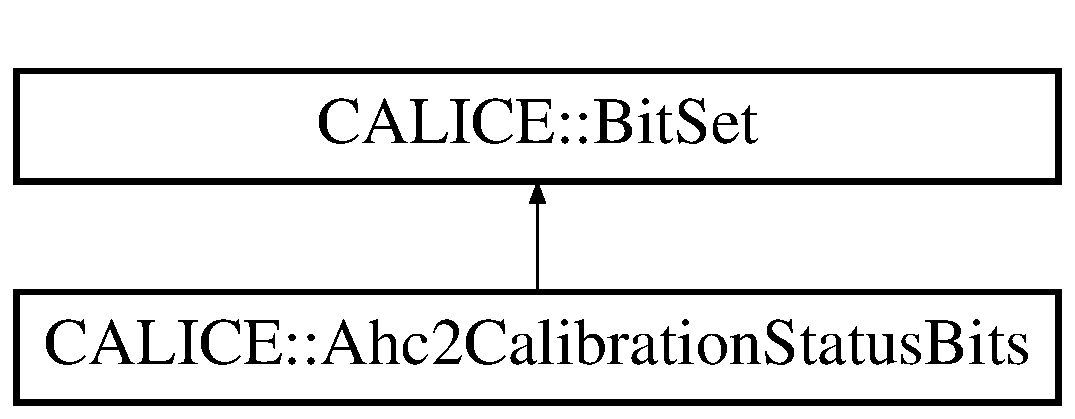
\includegraphics[height=2.000000cm]{classCALICE_1_1Ahc2CalibrationStatusBits}
\end{center}
\end{figure}
\subsection*{Public Member Functions}
\begin{DoxyCompactItemize}
\item 
{\bf Ahc2\-Calibration\-Status\-Bits} ()
\begin{DoxyCompactList}\small\item\em standard constructor \end{DoxyCompactList}\item 
{\bf Ahc2\-Calibration\-Status\-Bits} (const int value)
\begin{DoxyCompactList}\small\item\em constructor with initialisaton of the the bits \end{DoxyCompactList}\item 
bool {\bfseries is\-Dead} () const \label{classCALICE_1_1Ahc2CalibrationStatusBits_ac0d15dd4f791b91c9c6ad5fe41fd6cc3}

\item 
bool {\bfseries no\-Pedestal} () const \label{classCALICE_1_1Ahc2CalibrationStatusBits_a6edc0dfbb241566136c21ab01669fc51}

\item 
bool {\bfseries no\-Pedestal\-Memory\-Cell\-Offset} () const \label{classCALICE_1_1Ahc2CalibrationStatusBits_af7272c75ed01acdb4c14157610a88f2f}

\item 
bool {\bfseries no\-Low\-Gain\-Pedestal} () const \label{classCALICE_1_1Ahc2CalibrationStatusBits_a2a2377dba3c46ceb660bbc670f87af04}

\item 
bool {\bfseries no\-Low\-Gain\-Pedestal\-Memory\-Cell\-Offset} () const \label{classCALICE_1_1Ahc2CalibrationStatusBits_acfbded3e6c17cd44b083cfb38b41e553}

\item 
bool {\bfseries no\-Temperature} () const \label{classCALICE_1_1Ahc2CalibrationStatusBits_a9fb04b1b5428592afefa219ecf9aec49}

\item 
bool {\bfseries is\-New\-I\-T\-E\-P} () const \label{classCALICE_1_1Ahc2CalibrationStatusBits_a6fb3027bf68829d150668f0184423ecd}

\item 
bool {\bfseries M\-I\-P\-Constant\-Is\-Default} () const \label{classCALICE_1_1Ahc2CalibrationStatusBits_af11386a9a08c65042522c4b2af4f9f6f}

\item 
bool {\bfseries M\-I\-P\-Slope\-Is\-Default} () const \label{classCALICE_1_1Ahc2CalibrationStatusBits_a50b4fe7b0aa00e0483bb59a2d99af59f}

\item 
bool {\bfseries gain\-Constant\-Is\-Default} () const \label{classCALICE_1_1Ahc2CalibrationStatusBits_a7098ed6fd937b62c040c929eb40682d1}

\item 
bool {\bfseries gain\-Slope\-Is\-Default} () const \label{classCALICE_1_1Ahc2CalibrationStatusBits_a4bb22c8217cdf4b6b0ac9c181aedb3a3}

\item 
bool {\bfseries inter\-Calibration\-Is\-Default} () const \label{classCALICE_1_1Ahc2CalibrationStatusBits_aa90445a6de7f1f35b3e8e1ffe34299a9}

\item 
bool {\bfseries Physics\-Calib\-I\-C\-Is\-Default} () const \label{classCALICE_1_1Ahc2CalibrationStatusBits_a5cee89c4a70a9e196bae203818920bc4}

\item 
bool {\bfseries saturation\-Parameters\-Is\-Default} () const \label{classCALICE_1_1Ahc2CalibrationStatusBits_a838584c262cfbccea7969744e968e563}

\item 
bool {\bfseries Time\-Slopes\-Parameters\-Is\-Default} () const \label{classCALICE_1_1Ahc2CalibrationStatusBits_a84bb230b2a5a83cc168640aef3675027}

\item 
bool {\bfseries Time\-Offset\-Parameters\-Is\-Default} () const \label{classCALICE_1_1Ahc2CalibrationStatusBits_a6018de75f0dbf2df18d67e8e66fea6c0}

\item 
bool {\bfseries Time\-Offset\-Mem\-Cell\-Even\-Parameters\-Is\-Default} () const \label{classCALICE_1_1Ahc2CalibrationStatusBits_af303d33a62599ba69b0ceb200fd79636}

\item 
bool {\bfseries Time\-Offset\-Mem\-Cell\-Odd\-Parameters\-Is\-Default} () const \label{classCALICE_1_1Ahc2CalibrationStatusBits_a1288fac47b6d8e8af90e7734611abfb2}

\item 
bool {\bfseries Time\-Offset\-Mem\-Cell\-Even\-Buffer\-Even\-Event\-Even\-Parameters\-Is\-Default} () const \label{classCALICE_1_1Ahc2CalibrationStatusBits_abad8297ffd47204d37da102e8cdf0544}

\item 
bool {\bfseries Time\-Offset\-Mem\-Cell\-Odd\-Buffer\-Even\-Event\-Odd\-Parameters\-Is\-Default} () const \label{classCALICE_1_1Ahc2CalibrationStatusBits_a9f1129a9f6663d589af8bf6930d8f1eb}

\item 
bool {\bfseries Time\-Offset\-Mem\-Cell\-Even\-Buffer\-Odd\-Event\-Even\-Parameters\-Is\-Default} () const \label{classCALICE_1_1Ahc2CalibrationStatusBits_ac51b8d18c3ed74de8add3db7b8c214a1}

\item 
bool {\bfseries Time\-Offset\-Mem\-Cell\-Odd\-Buffer\-Odd\-Event\-Odd\-Parameters\-Is\-Default} () const \label{classCALICE_1_1Ahc2CalibrationStatusBits_a6454643883a416920df36d2be71702f4}

\item 
bool {\bfseries Occupancy\-Bxid\-Even\-High\-Gain\-Parameters\-Is\-Default} () const \label{classCALICE_1_1Ahc2CalibrationStatusBits_adc225f8763ea2bc1f3c15b2829a3d540}

\item 
bool {\bfseries Occupancy\-Bxid\-Even\-Low\-Gain\-Parameters\-Is\-Default} () const \label{classCALICE_1_1Ahc2CalibrationStatusBits_ad536d122a837b7dbd06ab0135b2534b7}

\item 
bool {\bfseries Occupancy\-Bxid\-Odd\-High\-Gain\-Parameters\-Is\-Default} () const \label{classCALICE_1_1Ahc2CalibrationStatusBits_a7db60192fcf8ec3f69038350d0ea2002}

\item 
bool {\bfseries Occupancy\-Bxid\-Odd\-Low\-Gain\-Parameters\-Is\-Default} () const \label{classCALICE_1_1Ahc2CalibrationStatusBits_a62dc3097c52f7ec47e20ea2e9f7571d9}

\item 
bool {\bfseries has\-Default} () const \label{classCALICE_1_1Ahc2CalibrationStatusBits_abc660f877930fa42c2e8527dcff5d2d7}

\item 
bool {\bfseries M\-I\-P\-Constant\-Is\-Scaled} () const \label{classCALICE_1_1Ahc2CalibrationStatusBits_a7c8965a803ecec5750d1c230d3276ce9}

\item 
bool {\bfseries M\-I\-P\-Slope\-Is\-Scaled} () const \label{classCALICE_1_1Ahc2CalibrationStatusBits_a5ab7245b3e09f28776a5456796e7fa2e}

\item 
bool {\bfseries gain\-Constant\-Is\-Scaled} () const \label{classCALICE_1_1Ahc2CalibrationStatusBits_a4590015de61eadec69155b6f052785ef}

\item 
bool {\bfseries gain\-Slope\-Is\-Scaled} () const \label{classCALICE_1_1Ahc2CalibrationStatusBits_a0f661aabae4ebbc614e5cd64f5494997}

\item 
bool {\bfseries inter\-Calibration\-Is\-Scaled} () const \label{classCALICE_1_1Ahc2CalibrationStatusBits_a05d6c638e0e7f499f8b767deba52b7ef}

\item 
bool {\bfseries Physics\-Calib\-I\-C\-Is\-Scaled} () const \label{classCALICE_1_1Ahc2CalibrationStatusBits_a9cd5210e7e5a264e30965e2014d9eedc}

\item 
bool {\bfseries has\-Scaled} () const \label{classCALICE_1_1Ahc2CalibrationStatusBits_a7722b3dc5a233bcb4390f62f809dd56c}

\item 
void {\bfseries set\-Dead} (const bool state=true)\label{classCALICE_1_1Ahc2CalibrationStatusBits_a7086d3e5eb96292e47cd896457986780}

\item 
void {\bfseries set\-No\-Pedestal} (const bool state=true)\label{classCALICE_1_1Ahc2CalibrationStatusBits_a759b14ec17dfa8266058ee01400fec4e}

\item 
void {\bfseries set\-No\-Pedestal\-Memory\-Cell\-Offset} (const bool state=true)\label{classCALICE_1_1Ahc2CalibrationStatusBits_afeba8093ee394e62aa5efa35231844ef}

\item 
void {\bfseries set\-No\-Low\-Gain\-Pedestal} (const bool state=true)\label{classCALICE_1_1Ahc2CalibrationStatusBits_a70af0a84f3fc458957895508bbf235cf}

\item 
void {\bfseries set\-No\-Low\-Gain\-Pedestal\-Memory\-Cell\-Offset} (const bool state=true)\label{classCALICE_1_1Ahc2CalibrationStatusBits_a01fd34e07c5af526282d4b4fe47d4d78}

\item 
void {\bfseries set\-No\-Temperature} (const bool state=true)\label{classCALICE_1_1Ahc2CalibrationStatusBits_aa3c37fe71a8a3727699dda63f145d08e}

\item 
void {\bfseries setis\-New\-I\-T\-E\-P} (const bool state=true)\label{classCALICE_1_1Ahc2CalibrationStatusBits_a618d44185909927e61bf308b71ab3f02}

\item 
void {\bfseries set\-M\-I\-P\-Constant\-Default} (const bool state=true)\label{classCALICE_1_1Ahc2CalibrationStatusBits_a563abd517939b634e2d4a032476c5f50}

\item 
void {\bfseries set\-M\-I\-P\-Slope\-Default} (const bool state=true)\label{classCALICE_1_1Ahc2CalibrationStatusBits_a93d2fb3dbcae45735a46faaea352c39b}

\item 
void {\bfseries set\-Gain\-Constant\-Default} (const bool state=true)\label{classCALICE_1_1Ahc2CalibrationStatusBits_ab4b50418d9b99b263842832f41cf6d8f}

\item 
void {\bfseries set\-Gain\-Slope\-Default} (const bool state=true)\label{classCALICE_1_1Ahc2CalibrationStatusBits_a8a9da4c25b8317896497ec216f831fc6}

\item 
void {\bfseries set\-Inter\-Calibration\-Default} (const bool state=true)\label{classCALICE_1_1Ahc2CalibrationStatusBits_adb01ce4e46929b52e7fb89dcc8e0d89b}

\item 
void {\bfseries set\-Physics\-Calib\-I\-C\-Default} (const bool state=true)\label{classCALICE_1_1Ahc2CalibrationStatusBits_a7b51b16ade7fdf0803b968e41e94303e}

\item 
void {\bfseries set\-Saturation\-Parameters\-Default} (const bool state=true)\label{classCALICE_1_1Ahc2CalibrationStatusBits_a215a322f8475633417f9727e1f073908}

\item 
void {\bfseries set\-Time\-Slopes\-Parameters\-Default} (const bool state=true)\label{classCALICE_1_1Ahc2CalibrationStatusBits_a50e4cfea2375a925be6e50fe82eda241}

\item 
void {\bfseries set\-Time\-Offset\-Parameters\-Default} (const bool state=true)\label{classCALICE_1_1Ahc2CalibrationStatusBits_ae14785cd6fda41550e221d1707613459}

\item 
void {\bfseries set\-Time\-Offset\-Mem\-Cell\-Even\-Parameters\-Default} (const bool state=true)\label{classCALICE_1_1Ahc2CalibrationStatusBits_abc392df434d705b639cb38bda371a9ca}

\item 
void {\bfseries set\-Time\-Offset\-Mem\-Cell\-Odd\-Parameters\-Default} (const bool state=true)\label{classCALICE_1_1Ahc2CalibrationStatusBits_a3777b802882728e9d84f11df1af1d905}

\item 
void {\bfseries set\-Time\-Offset\-Mem\-Cell\-Even\-Buffer\-Even\-Event\-Even\-Parameters\-Default} (const bool state=true)\label{classCALICE_1_1Ahc2CalibrationStatusBits_af810f08499af667c69cb5f8cb1b1b0de}

\item 
void {\bfseries set\-Time\-Offset\-Mem\-Cell\-Odd\-Buffer\-Even\-Event\-Odd\-Parameters\-Default} (const bool state=true)\label{classCALICE_1_1Ahc2CalibrationStatusBits_a0569988993b5e4fcfe117d9bd3f53481}

\item 
void {\bfseries set\-Time\-Offset\-Mem\-Cell\-Even\-Buffer\-Odd\-Event\-Even\-Parameters\-Default} (const bool state=true)\label{classCALICE_1_1Ahc2CalibrationStatusBits_a2731a934de734be7281e2eb2d2ceffb1}

\item 
void {\bfseries set\-Time\-Offset\-Mem\-Cell\-Odd\-Buffer\-Odd\-Event\-Odd\-Parameters\-Default} (const bool state=true)\label{classCALICE_1_1Ahc2CalibrationStatusBits_a694933ed78c4571c849c97224cfb19c3}

\item 
void {\bfseries set\-Occupancy\-Bxid\-Even\-High\-Gain\-Parameters\-Default} (const bool state=true)\label{classCALICE_1_1Ahc2CalibrationStatusBits_a9fdd3b006fe62f23a8f19b235b72c24c}

\item 
void {\bfseries set\-Occupancy\-Bxid\-Even\-Low\-Gain\-Parameters\-Default} (const bool state=true)\label{classCALICE_1_1Ahc2CalibrationStatusBits_aeafe638ce0901fca25926fb6968ee0af}

\item 
void {\bfseries set\-Occupancy\-Bxid\-Odd\-High\-Gain\-Parameters\-Default} (const bool state=true)\label{classCALICE_1_1Ahc2CalibrationStatusBits_a4b5f518bd09d8aeac7060bffcf1ad24e}

\item 
void {\bfseries set\-Occupancy\-Bxid\-Odd\-Low\-Gain\-Parameters\-Default} (const bool state=true)\label{classCALICE_1_1Ahc2CalibrationStatusBits_a75582cc26346cad5f37843dbade6cafa}

\item 
void {\bfseries set\-M\-I\-P\-Constant\-Scaled} (const bool state=true)\label{classCALICE_1_1Ahc2CalibrationStatusBits_a7b90ee374016c59fe0931a1e42840941}

\item 
void {\bfseries set\-M\-I\-P\-Slope\-Scaled} (const bool state=true)\label{classCALICE_1_1Ahc2CalibrationStatusBits_a2e2221cf01d5766f3f3ff1d66fc9364a}

\item 
void {\bfseries set\-Gain\-Constant\-Scaled} (const bool state=true)\label{classCALICE_1_1Ahc2CalibrationStatusBits_ae6dcfafd7074e5915ae7adb2e7c2101d}

\item 
void {\bfseries set\-Gain\-Slope\-Scaled} (const bool state=true)\label{classCALICE_1_1Ahc2CalibrationStatusBits_a7c8db965152f0f13fb2d0b2278136288}

\item 
void {\bfseries set\-Inter\-Calibration\-Scaled} (const bool state=true)\label{classCALICE_1_1Ahc2CalibrationStatusBits_ad918faf4d0f89479592661f385559ec6}

\item 
void {\bfseries set\-Physics\-Calib\-I\-C\-Scaled} (const bool state=true)\label{classCALICE_1_1Ahc2CalibrationStatusBits_a214becc89abb9ebfaa913884f848d59c}

\end{DoxyCompactItemize}
\subsection*{Protected Types}
\begin{DoxyCompactItemize}
\item 
enum {\bf E\-Ahc2\-Calibration\-Status\-Bit\-No} \{ \\*
{\bf k\-Is\-Dead}, 
{\bf k\-No\-Pedestal}, 
{\bf k\-No\-Pedestal\-Memory\-Cell\-Offset}, 
{\bf k\-No\-Low\-Gain\-Pedestal}, 
\\*
{\bf k\-No\-Low\-Gain\-Pedestal\-Memory\-Cell\-Offset}, 
{\bf k\-No\-Temperature}, 
{\bf kis\-New\-I\-T\-E\-P}, 
{\bf k\-M\-I\-P\-Constant\-Is\-Default}, 
\\*
{\bf k\-M\-I\-P\-Slope\-Is\-Default}, 
{\bf k\-Gain\-Constant\-Is\-Default}, 
{\bf k\-Gain\-Slope\-Is\-Default}, 
{\bf k\-Inter\-Calibration\-Is\-Default}, 
\\*
{\bf k\-Physics\-Calib\-I\-C\-Is\-Default}, 
{\bf k\-Saturation\-Parameters\-Is\-Default}, 
{\bf k\-Time\-Slopes\-Parameters\-Is\-Default}, 
{\bf k\-Time\-Offset\-Parameters\-Is\-Default}, 
\\*
{\bf k\-Time\-Offset\-Mem\-Cell\-Even\-Parameters\-Is\-Default}, 
{\bf k\-Time\-Offset\-Mem\-Cell\-Odd\-Parameters\-Is\-Default}, 
{\bfseries k\-Time\-Offset\-Mem\-Cell\-Even\-Buffer\-Even\-Event\-Even\-Parameters\-Is\-Default}, 
{\bfseries k\-Time\-Offset\-Mem\-Cell\-Odd\-Buffer\-Even\-Event\-Odd\-Parameters\-Is\-Default}, 
\\*
{\bfseries k\-Time\-Offset\-Mem\-Cell\-Even\-Buffer\-Odd\-Event\-Even\-Parameters\-Is\-Default}, 
{\bfseries k\-Time\-Offset\-Mem\-Cell\-Odd\-Buffer\-Odd\-Event\-Odd\-Parameters\-Is\-Default}, 
{\bfseries k\-Occupancy\-Bxid\-Even\-High\-Gain\-Parameters\-Is\-Default}, 
{\bfseries k\-Occupancy\-Bxid\-Even\-Low\-Gain\-Parameters\-Is\-Default}, 
\\*
{\bfseries k\-Occupancy\-Bxid\-Odd\-High\-Gain\-Parameters\-Is\-Default}, 
{\bfseries k\-Occupancy\-Bxid\-Odd\-Low\-Gain\-Parameters\-Is\-Default}, 
{\bf k\-M\-I\-P\-Constant\-Is\-Scaled}, 
{\bf k\-M\-I\-P\-Slope\-Is\-Scaled}, 
\\*
{\bf k\-Gain\-Constant\-Is\-Scaled}, 
{\bf k\-Gain\-Slope\-Is\-Scaled}, 
{\bf k\-Inter\-Calibration\-Is\-Scaled}, 
{\bf k\-Physics\-Calib\-I\-C\-Is\-Scaled}, 
\\*
{\bfseries k\-Number\-Of\-Bits}
 \}
\end{DoxyCompactItemize}
\subsection*{Additional Inherited Members}


\subsection{Detailed Description}
Bit set to describe the Ahc2 Calibration Status. 

\begin{DoxyAuthor}{Author}
E.\-Brianne 
\end{DoxyAuthor}
\begin{DoxyDate}{Date}
Novemeber 2015 
\end{DoxyDate}
\begin{DoxyVersion}{Version}
1.\-0 
\end{DoxyVersion}


Definition at line 16 of file Ahc2\-Calibration\-Status\-Bits.\-hh.



\subsection{Member Enumeration Documentation}
\index{C\-A\-L\-I\-C\-E\-::\-Ahc2\-Calibration\-Status\-Bits@{C\-A\-L\-I\-C\-E\-::\-Ahc2\-Calibration\-Status\-Bits}!E\-Ahc2\-Calibration\-Status\-Bit\-No@{E\-Ahc2\-Calibration\-Status\-Bit\-No}}
\index{E\-Ahc2\-Calibration\-Status\-Bit\-No@{E\-Ahc2\-Calibration\-Status\-Bit\-No}!CALICE::Ahc2CalibrationStatusBits@{C\-A\-L\-I\-C\-E\-::\-Ahc2\-Calibration\-Status\-Bits}}
\subsubsection[{E\-Ahc2\-Calibration\-Status\-Bit\-No}]{\setlength{\rightskip}{0pt plus 5cm}enum {\bf C\-A\-L\-I\-C\-E\-::\-Ahc2\-Calibration\-Status\-Bits\-::\-E\-Ahc2\-Calibration\-Status\-Bit\-No}\hspace{0.3cm}{\ttfamily [protected]}}\label{classCALICE_1_1Ahc2CalibrationStatusBits_ad3344194d3554ee4db5684dcffc0125a}
\begin{Desc}
\item[Enumerator]\par
\begin{description}
\index{k\-Is\-Dead@{k\-Is\-Dead}!C\-A\-L\-I\-C\-E\-::\-Ahc2\-Calibration\-Status\-Bits@{C\-A\-L\-I\-C\-E\-::\-Ahc2\-Calibration\-Status\-Bits}}\index{C\-A\-L\-I\-C\-E\-::\-Ahc2\-Calibration\-Status\-Bits@{C\-A\-L\-I\-C\-E\-::\-Ahc2\-Calibration\-Status\-Bits}!k\-Is\-Dead@{k\-Is\-Dead}}\item[{\em 
k\-Is\-Dead\label{classCALICE_1_1Ahc2CalibrationStatusBits_ad3344194d3554ee4db5684dcffc0125aa7e34ebc884839af14f752026f2e0760a}
}]this cell is flagged dead \index{k\-No\-Pedestal@{k\-No\-Pedestal}!C\-A\-L\-I\-C\-E\-::\-Ahc2\-Calibration\-Status\-Bits@{C\-A\-L\-I\-C\-E\-::\-Ahc2\-Calibration\-Status\-Bits}}\index{C\-A\-L\-I\-C\-E\-::\-Ahc2\-Calibration\-Status\-Bits@{C\-A\-L\-I\-C\-E\-::\-Ahc2\-Calibration\-Status\-Bits}!k\-No\-Pedestal@{k\-No\-Pedestal}}\item[{\em 
k\-No\-Pedestal\label{classCALICE_1_1Ahc2CalibrationStatusBits_ad3344194d3554ee4db5684dcffc0125aae03d7c52fdaa22d8868acd451b9f36d8}
}]no pedestal value available \index{k\-No\-Pedestal\-Memory\-Cell\-Offset@{k\-No\-Pedestal\-Memory\-Cell\-Offset}!C\-A\-L\-I\-C\-E\-::\-Ahc2\-Calibration\-Status\-Bits@{C\-A\-L\-I\-C\-E\-::\-Ahc2\-Calibration\-Status\-Bits}}\index{C\-A\-L\-I\-C\-E\-::\-Ahc2\-Calibration\-Status\-Bits@{C\-A\-L\-I\-C\-E\-::\-Ahc2\-Calibration\-Status\-Bits}!k\-No\-Pedestal\-Memory\-Cell\-Offset@{k\-No\-Pedestal\-Memory\-Cell\-Offset}}\item[{\em 
k\-No\-Pedestal\-Memory\-Cell\-Offset\label{classCALICE_1_1Ahc2CalibrationStatusBits_ad3344194d3554ee4db5684dcffc0125aade374f28ae6ed9a926b1eece6af0437d}
}]no pedestal value available \index{k\-No\-Low\-Gain\-Pedestal@{k\-No\-Low\-Gain\-Pedestal}!C\-A\-L\-I\-C\-E\-::\-Ahc2\-Calibration\-Status\-Bits@{C\-A\-L\-I\-C\-E\-::\-Ahc2\-Calibration\-Status\-Bits}}\index{C\-A\-L\-I\-C\-E\-::\-Ahc2\-Calibration\-Status\-Bits@{C\-A\-L\-I\-C\-E\-::\-Ahc2\-Calibration\-Status\-Bits}!k\-No\-Low\-Gain\-Pedestal@{k\-No\-Low\-Gain\-Pedestal}}\item[{\em 
k\-No\-Low\-Gain\-Pedestal\label{classCALICE_1_1Ahc2CalibrationStatusBits_ad3344194d3554ee4db5684dcffc0125aa478e51d07e40f2332cd797a04ab1baf2}
}]no pedestal value available \index{k\-No\-Low\-Gain\-Pedestal\-Memory\-Cell\-Offset@{k\-No\-Low\-Gain\-Pedestal\-Memory\-Cell\-Offset}!C\-A\-L\-I\-C\-E\-::\-Ahc2\-Calibration\-Status\-Bits@{C\-A\-L\-I\-C\-E\-::\-Ahc2\-Calibration\-Status\-Bits}}\index{C\-A\-L\-I\-C\-E\-::\-Ahc2\-Calibration\-Status\-Bits@{C\-A\-L\-I\-C\-E\-::\-Ahc2\-Calibration\-Status\-Bits}!k\-No\-Low\-Gain\-Pedestal\-Memory\-Cell\-Offset@{k\-No\-Low\-Gain\-Pedestal\-Memory\-Cell\-Offset}}\item[{\em 
k\-No\-Low\-Gain\-Pedestal\-Memory\-Cell\-Offset\label{classCALICE_1_1Ahc2CalibrationStatusBits_ad3344194d3554ee4db5684dcffc0125aad3c73b70bf73ce7cbf4cf13e9ef8d84d}
}]no pedestal value available \index{k\-No\-Temperature@{k\-No\-Temperature}!C\-A\-L\-I\-C\-E\-::\-Ahc2\-Calibration\-Status\-Bits@{C\-A\-L\-I\-C\-E\-::\-Ahc2\-Calibration\-Status\-Bits}}\index{C\-A\-L\-I\-C\-E\-::\-Ahc2\-Calibration\-Status\-Bits@{C\-A\-L\-I\-C\-E\-::\-Ahc2\-Calibration\-Status\-Bits}!k\-No\-Temperature@{k\-No\-Temperature}}\item[{\em 
k\-No\-Temperature\label{classCALICE_1_1Ahc2CalibrationStatusBits_ad3344194d3554ee4db5684dcffc0125aa607335442ed069c70b528de9962b81ee}
}]no temperature value available \index{kis\-New\-I\-T\-E\-P@{kis\-New\-I\-T\-E\-P}!C\-A\-L\-I\-C\-E\-::\-Ahc2\-Calibration\-Status\-Bits@{C\-A\-L\-I\-C\-E\-::\-Ahc2\-Calibration\-Status\-Bits}}\index{C\-A\-L\-I\-C\-E\-::\-Ahc2\-Calibration\-Status\-Bits@{C\-A\-L\-I\-C\-E\-::\-Ahc2\-Calibration\-Status\-Bits}!kis\-New\-I\-T\-E\-P@{kis\-New\-I\-T\-E\-P}}\item[{\em 
kis\-New\-I\-T\-E\-P\label{classCALICE_1_1Ahc2CalibrationStatusBits_ad3344194d3554ee4db5684dcffc0125aac117f122621d0afb9f8877dba5a0aa02}
}]is a new I\-T\-E\-P Tile \index{k\-M\-I\-P\-Constant\-Is\-Default@{k\-M\-I\-P\-Constant\-Is\-Default}!C\-A\-L\-I\-C\-E\-::\-Ahc2\-Calibration\-Status\-Bits@{C\-A\-L\-I\-C\-E\-::\-Ahc2\-Calibration\-Status\-Bits}}\index{C\-A\-L\-I\-C\-E\-::\-Ahc2\-Calibration\-Status\-Bits@{C\-A\-L\-I\-C\-E\-::\-Ahc2\-Calibration\-Status\-Bits}!k\-M\-I\-P\-Constant\-Is\-Default@{k\-M\-I\-P\-Constant\-Is\-Default}}\item[{\em 
k\-M\-I\-P\-Constant\-Is\-Default\label{classCALICE_1_1Ahc2CalibrationStatusBits_ad3344194d3554ee4db5684dcffc0125aa63fd30db886fb78bc405e0b01561ecc3}
}]the default M\-I\-P constant was used \index{k\-M\-I\-P\-Slope\-Is\-Default@{k\-M\-I\-P\-Slope\-Is\-Default}!C\-A\-L\-I\-C\-E\-::\-Ahc2\-Calibration\-Status\-Bits@{C\-A\-L\-I\-C\-E\-::\-Ahc2\-Calibration\-Status\-Bits}}\index{C\-A\-L\-I\-C\-E\-::\-Ahc2\-Calibration\-Status\-Bits@{C\-A\-L\-I\-C\-E\-::\-Ahc2\-Calibration\-Status\-Bits}!k\-M\-I\-P\-Slope\-Is\-Default@{k\-M\-I\-P\-Slope\-Is\-Default}}\item[{\em 
k\-M\-I\-P\-Slope\-Is\-Default\label{classCALICE_1_1Ahc2CalibrationStatusBits_ad3344194d3554ee4db5684dcffc0125aa237f11a760410e8f1071c4dc583df52b}
}]the default M\-I\-P slope was used \index{k\-Gain\-Constant\-Is\-Default@{k\-Gain\-Constant\-Is\-Default}!C\-A\-L\-I\-C\-E\-::\-Ahc2\-Calibration\-Status\-Bits@{C\-A\-L\-I\-C\-E\-::\-Ahc2\-Calibration\-Status\-Bits}}\index{C\-A\-L\-I\-C\-E\-::\-Ahc2\-Calibration\-Status\-Bits@{C\-A\-L\-I\-C\-E\-::\-Ahc2\-Calibration\-Status\-Bits}!k\-Gain\-Constant\-Is\-Default@{k\-Gain\-Constant\-Is\-Default}}\item[{\em 
k\-Gain\-Constant\-Is\-Default\label{classCALICE_1_1Ahc2CalibrationStatusBits_ad3344194d3554ee4db5684dcffc0125aad9cd362824e536d4b55b6373817c92db}
}]the default gain constant was used \index{k\-Gain\-Slope\-Is\-Default@{k\-Gain\-Slope\-Is\-Default}!C\-A\-L\-I\-C\-E\-::\-Ahc2\-Calibration\-Status\-Bits@{C\-A\-L\-I\-C\-E\-::\-Ahc2\-Calibration\-Status\-Bits}}\index{C\-A\-L\-I\-C\-E\-::\-Ahc2\-Calibration\-Status\-Bits@{C\-A\-L\-I\-C\-E\-::\-Ahc2\-Calibration\-Status\-Bits}!k\-Gain\-Slope\-Is\-Default@{k\-Gain\-Slope\-Is\-Default}}\item[{\em 
k\-Gain\-Slope\-Is\-Default\label{classCALICE_1_1Ahc2CalibrationStatusBits_ad3344194d3554ee4db5684dcffc0125aa217bfa9d316f56996b6780ef43784ee7}
}]the default gain slope was used \index{k\-Inter\-Calibration\-Is\-Default@{k\-Inter\-Calibration\-Is\-Default}!C\-A\-L\-I\-C\-E\-::\-Ahc2\-Calibration\-Status\-Bits@{C\-A\-L\-I\-C\-E\-::\-Ahc2\-Calibration\-Status\-Bits}}\index{C\-A\-L\-I\-C\-E\-::\-Ahc2\-Calibration\-Status\-Bits@{C\-A\-L\-I\-C\-E\-::\-Ahc2\-Calibration\-Status\-Bits}!k\-Inter\-Calibration\-Is\-Default@{k\-Inter\-Calibration\-Is\-Default}}\item[{\em 
k\-Inter\-Calibration\-Is\-Default\label{classCALICE_1_1Ahc2CalibrationStatusBits_ad3344194d3554ee4db5684dcffc0125aa86728ec4fb7915a15e4893ebc8aef3c1}
}]the default inter-\/calibration constant was used \index{k\-Physics\-Calib\-I\-C\-Is\-Default@{k\-Physics\-Calib\-I\-C\-Is\-Default}!C\-A\-L\-I\-C\-E\-::\-Ahc2\-Calibration\-Status\-Bits@{C\-A\-L\-I\-C\-E\-::\-Ahc2\-Calibration\-Status\-Bits}}\index{C\-A\-L\-I\-C\-E\-::\-Ahc2\-Calibration\-Status\-Bits@{C\-A\-L\-I\-C\-E\-::\-Ahc2\-Calibration\-Status\-Bits}!k\-Physics\-Calib\-I\-C\-Is\-Default@{k\-Physics\-Calib\-I\-C\-Is\-Default}}\item[{\em 
k\-Physics\-Calib\-I\-C\-Is\-Default\label{classCALICE_1_1Ahc2CalibrationStatusBits_ad3344194d3554ee4db5684dcffc0125aade97e2ae931cae9636c5395a8d612253}
}]the default inter-\/calibration physics/calib constant was used \index{k\-Saturation\-Parameters\-Is\-Default@{k\-Saturation\-Parameters\-Is\-Default}!C\-A\-L\-I\-C\-E\-::\-Ahc2\-Calibration\-Status\-Bits@{C\-A\-L\-I\-C\-E\-::\-Ahc2\-Calibration\-Status\-Bits}}\index{C\-A\-L\-I\-C\-E\-::\-Ahc2\-Calibration\-Status\-Bits@{C\-A\-L\-I\-C\-E\-::\-Ahc2\-Calibration\-Status\-Bits}!k\-Saturation\-Parameters\-Is\-Default@{k\-Saturation\-Parameters\-Is\-Default}}\item[{\em 
k\-Saturation\-Parameters\-Is\-Default\label{classCALICE_1_1Ahc2CalibrationStatusBits_ad3344194d3554ee4db5684dcffc0125aacdd3ebd3a6ab6e06c921564c398c3140}
}]the default saturation parameters was used \index{k\-Time\-Slopes\-Parameters\-Is\-Default@{k\-Time\-Slopes\-Parameters\-Is\-Default}!C\-A\-L\-I\-C\-E\-::\-Ahc2\-Calibration\-Status\-Bits@{C\-A\-L\-I\-C\-E\-::\-Ahc2\-Calibration\-Status\-Bits}}\index{C\-A\-L\-I\-C\-E\-::\-Ahc2\-Calibration\-Status\-Bits@{C\-A\-L\-I\-C\-E\-::\-Ahc2\-Calibration\-Status\-Bits}!k\-Time\-Slopes\-Parameters\-Is\-Default@{k\-Time\-Slopes\-Parameters\-Is\-Default}}\item[{\em 
k\-Time\-Slopes\-Parameters\-Is\-Default\label{classCALICE_1_1Ahc2CalibrationStatusBits_ad3344194d3554ee4db5684dcffc0125aa364d9be2e09985c9291aeb432b527f3f}
}]the default time slopes parameters was used \index{k\-Time\-Offset\-Parameters\-Is\-Default@{k\-Time\-Offset\-Parameters\-Is\-Default}!C\-A\-L\-I\-C\-E\-::\-Ahc2\-Calibration\-Status\-Bits@{C\-A\-L\-I\-C\-E\-::\-Ahc2\-Calibration\-Status\-Bits}}\index{C\-A\-L\-I\-C\-E\-::\-Ahc2\-Calibration\-Status\-Bits@{C\-A\-L\-I\-C\-E\-::\-Ahc2\-Calibration\-Status\-Bits}!k\-Time\-Offset\-Parameters\-Is\-Default@{k\-Time\-Offset\-Parameters\-Is\-Default}}\item[{\em 
k\-Time\-Offset\-Parameters\-Is\-Default\label{classCALICE_1_1Ahc2CalibrationStatusBits_ad3344194d3554ee4db5684dcffc0125aa5aa475c80a32ac4e0b79fb1a52eee2e4}
}]the default time pedestal parameters was used \index{k\-Time\-Offset\-Mem\-Cell\-Even\-Parameters\-Is\-Default@{k\-Time\-Offset\-Mem\-Cell\-Even\-Parameters\-Is\-Default}!C\-A\-L\-I\-C\-E\-::\-Ahc2\-Calibration\-Status\-Bits@{C\-A\-L\-I\-C\-E\-::\-Ahc2\-Calibration\-Status\-Bits}}\index{C\-A\-L\-I\-C\-E\-::\-Ahc2\-Calibration\-Status\-Bits@{C\-A\-L\-I\-C\-E\-::\-Ahc2\-Calibration\-Status\-Bits}!k\-Time\-Offset\-Mem\-Cell\-Even\-Parameters\-Is\-Default@{k\-Time\-Offset\-Mem\-Cell\-Even\-Parameters\-Is\-Default}}\item[{\em 
k\-Time\-Offset\-Mem\-Cell\-Even\-Parameters\-Is\-Default\label{classCALICE_1_1Ahc2CalibrationStatusBits_ad3344194d3554ee4db5684dcffc0125aa3dd77bf54d3a029ece2aa73931f01a63}
}]the default time pedestal parameters was used \index{k\-Time\-Offset\-Mem\-Cell\-Odd\-Parameters\-Is\-Default@{k\-Time\-Offset\-Mem\-Cell\-Odd\-Parameters\-Is\-Default}!C\-A\-L\-I\-C\-E\-::\-Ahc2\-Calibration\-Status\-Bits@{C\-A\-L\-I\-C\-E\-::\-Ahc2\-Calibration\-Status\-Bits}}\index{C\-A\-L\-I\-C\-E\-::\-Ahc2\-Calibration\-Status\-Bits@{C\-A\-L\-I\-C\-E\-::\-Ahc2\-Calibration\-Status\-Bits}!k\-Time\-Offset\-Mem\-Cell\-Odd\-Parameters\-Is\-Default@{k\-Time\-Offset\-Mem\-Cell\-Odd\-Parameters\-Is\-Default}}\item[{\em 
k\-Time\-Offset\-Mem\-Cell\-Odd\-Parameters\-Is\-Default\label{classCALICE_1_1Ahc2CalibrationStatusBits_ad3344194d3554ee4db5684dcffc0125aa1495dbacc434886c4f0d39ad8289c5a7}
}]the default time pedestal parameters was used \index{k\-M\-I\-P\-Constant\-Is\-Scaled@{k\-M\-I\-P\-Constant\-Is\-Scaled}!C\-A\-L\-I\-C\-E\-::\-Ahc2\-Calibration\-Status\-Bits@{C\-A\-L\-I\-C\-E\-::\-Ahc2\-Calibration\-Status\-Bits}}\index{C\-A\-L\-I\-C\-E\-::\-Ahc2\-Calibration\-Status\-Bits@{C\-A\-L\-I\-C\-E\-::\-Ahc2\-Calibration\-Status\-Bits}!k\-M\-I\-P\-Constant\-Is\-Scaled@{k\-M\-I\-P\-Constant\-Is\-Scaled}}\item[{\em 
k\-M\-I\-P\-Constant\-Is\-Scaled\label{classCALICE_1_1Ahc2CalibrationStatusBits_ad3344194d3554ee4db5684dcffc0125aa49718c13d54976247307d055598c7e9a}
}]the M\-I\-P constant was scaled \index{k\-M\-I\-P\-Slope\-Is\-Scaled@{k\-M\-I\-P\-Slope\-Is\-Scaled}!C\-A\-L\-I\-C\-E\-::\-Ahc2\-Calibration\-Status\-Bits@{C\-A\-L\-I\-C\-E\-::\-Ahc2\-Calibration\-Status\-Bits}}\index{C\-A\-L\-I\-C\-E\-::\-Ahc2\-Calibration\-Status\-Bits@{C\-A\-L\-I\-C\-E\-::\-Ahc2\-Calibration\-Status\-Bits}!k\-M\-I\-P\-Slope\-Is\-Scaled@{k\-M\-I\-P\-Slope\-Is\-Scaled}}\item[{\em 
k\-M\-I\-P\-Slope\-Is\-Scaled\label{classCALICE_1_1Ahc2CalibrationStatusBits_ad3344194d3554ee4db5684dcffc0125aae99bdb9a24e10aa18a3bc08475935e44}
}]the M\-I\-P slope was scaled \index{k\-Gain\-Constant\-Is\-Scaled@{k\-Gain\-Constant\-Is\-Scaled}!C\-A\-L\-I\-C\-E\-::\-Ahc2\-Calibration\-Status\-Bits@{C\-A\-L\-I\-C\-E\-::\-Ahc2\-Calibration\-Status\-Bits}}\index{C\-A\-L\-I\-C\-E\-::\-Ahc2\-Calibration\-Status\-Bits@{C\-A\-L\-I\-C\-E\-::\-Ahc2\-Calibration\-Status\-Bits}!k\-Gain\-Constant\-Is\-Scaled@{k\-Gain\-Constant\-Is\-Scaled}}\item[{\em 
k\-Gain\-Constant\-Is\-Scaled\label{classCALICE_1_1Ahc2CalibrationStatusBits_ad3344194d3554ee4db5684dcffc0125aab388bf74d2fe3e316e1133e59f2fbe99}
}]the gain constant was scaled \index{k\-Gain\-Slope\-Is\-Scaled@{k\-Gain\-Slope\-Is\-Scaled}!C\-A\-L\-I\-C\-E\-::\-Ahc2\-Calibration\-Status\-Bits@{C\-A\-L\-I\-C\-E\-::\-Ahc2\-Calibration\-Status\-Bits}}\index{C\-A\-L\-I\-C\-E\-::\-Ahc2\-Calibration\-Status\-Bits@{C\-A\-L\-I\-C\-E\-::\-Ahc2\-Calibration\-Status\-Bits}!k\-Gain\-Slope\-Is\-Scaled@{k\-Gain\-Slope\-Is\-Scaled}}\item[{\em 
k\-Gain\-Slope\-Is\-Scaled\label{classCALICE_1_1Ahc2CalibrationStatusBits_ad3344194d3554ee4db5684dcffc0125aa05c465cf012af018eb2c825c4e35ffbb}
}]the gain slope was scaled \index{k\-Inter\-Calibration\-Is\-Scaled@{k\-Inter\-Calibration\-Is\-Scaled}!C\-A\-L\-I\-C\-E\-::\-Ahc2\-Calibration\-Status\-Bits@{C\-A\-L\-I\-C\-E\-::\-Ahc2\-Calibration\-Status\-Bits}}\index{C\-A\-L\-I\-C\-E\-::\-Ahc2\-Calibration\-Status\-Bits@{C\-A\-L\-I\-C\-E\-::\-Ahc2\-Calibration\-Status\-Bits}!k\-Inter\-Calibration\-Is\-Scaled@{k\-Inter\-Calibration\-Is\-Scaled}}\item[{\em 
k\-Inter\-Calibration\-Is\-Scaled\label{classCALICE_1_1Ahc2CalibrationStatusBits_ad3344194d3554ee4db5684dcffc0125aa75faa095dc5c45002be7daa4690f7652}
}]the inter-\/calibration constant was scaled \index{k\-Physics\-Calib\-I\-C\-Is\-Scaled@{k\-Physics\-Calib\-I\-C\-Is\-Scaled}!C\-A\-L\-I\-C\-E\-::\-Ahc2\-Calibration\-Status\-Bits@{C\-A\-L\-I\-C\-E\-::\-Ahc2\-Calibration\-Status\-Bits}}\index{C\-A\-L\-I\-C\-E\-::\-Ahc2\-Calibration\-Status\-Bits@{C\-A\-L\-I\-C\-E\-::\-Ahc2\-Calibration\-Status\-Bits}!k\-Physics\-Calib\-I\-C\-Is\-Scaled@{k\-Physics\-Calib\-I\-C\-Is\-Scaled}}\item[{\em 
k\-Physics\-Calib\-I\-C\-Is\-Scaled\label{classCALICE_1_1Ahc2CalibrationStatusBits_ad3344194d3554ee4db5684dcffc0125aa7ae7f2e54b3f66f1ab06c56ecb90895c}
}]the inter-\/calibration physics/calib constant was scaled \end{description}
\end{Desc}


Definition at line 18 of file Ahc2\-Calibration\-Status\-Bits.\-hh.



\subsection{Constructor \& Destructor Documentation}
\index{C\-A\-L\-I\-C\-E\-::\-Ahc2\-Calibration\-Status\-Bits@{C\-A\-L\-I\-C\-E\-::\-Ahc2\-Calibration\-Status\-Bits}!Ahc2\-Calibration\-Status\-Bits@{Ahc2\-Calibration\-Status\-Bits}}
\index{Ahc2\-Calibration\-Status\-Bits@{Ahc2\-Calibration\-Status\-Bits}!CALICE::Ahc2CalibrationStatusBits@{C\-A\-L\-I\-C\-E\-::\-Ahc2\-Calibration\-Status\-Bits}}
\subsubsection[{Ahc2\-Calibration\-Status\-Bits}]{\setlength{\rightskip}{0pt plus 5cm}C\-A\-L\-I\-C\-E\-::\-Ahc2\-Calibration\-Status\-Bits\-::\-Ahc2\-Calibration\-Status\-Bits (
\begin{DoxyParamCaption}
{}
\end{DoxyParamCaption}
)\hspace{0.3cm}{\ttfamily [inline]}}\label{classCALICE_1_1Ahc2CalibrationStatusBits_a2fd762982236b0896d70ad153aea0bf4}


standard constructor 

all bits are off 

Definition at line 65 of file Ahc2\-Calibration\-Status\-Bits.\-hh.

\index{C\-A\-L\-I\-C\-E\-::\-Ahc2\-Calibration\-Status\-Bits@{C\-A\-L\-I\-C\-E\-::\-Ahc2\-Calibration\-Status\-Bits}!Ahc2\-Calibration\-Status\-Bits@{Ahc2\-Calibration\-Status\-Bits}}
\index{Ahc2\-Calibration\-Status\-Bits@{Ahc2\-Calibration\-Status\-Bits}!CALICE::Ahc2CalibrationStatusBits@{C\-A\-L\-I\-C\-E\-::\-Ahc2\-Calibration\-Status\-Bits}}
\subsubsection[{Ahc2\-Calibration\-Status\-Bits}]{\setlength{\rightskip}{0pt plus 5cm}C\-A\-L\-I\-C\-E\-::\-Ahc2\-Calibration\-Status\-Bits\-::\-Ahc2\-Calibration\-Status\-Bits (
\begin{DoxyParamCaption}
\item[{const int}]{value}
\end{DoxyParamCaption}
)\hspace{0.3cm}{\ttfamily [inline]}}\label{classCALICE_1_1Ahc2CalibrationStatusBits_a8bc250954688593df06a4b06b2b22915}


constructor with initialisaton of the the bits 


\begin{DoxyParams}[1]{Parameters}
\mbox{\tt in}  & {\em value} & bits to be set \\
\hline
\end{DoxyParams}


Definition at line 73 of file Ahc2\-Calibration\-Status\-Bits.\-hh.



The documentation for this class was generated from the following file\-:\begin{DoxyCompactItemize}
\item 
Ahc2\-Calibration\-Status\-Bits.\-hh\end{DoxyCompactItemize}

\section{C\-A\-L\-I\-C\-E\-:\-:Ahc2\-Hardware\-Connection Class Reference}
\label{classCALICE_1_1Ahc2HardwareConnection}\index{C\-A\-L\-I\-C\-E\-::\-Ahc2\-Hardware\-Connection@{C\-A\-L\-I\-C\-E\-::\-Ahc2\-Hardware\-Connection}}


Class to store int values for Hardware\-Connection plus integer cell index in L\-C\-I\-O.  




{\ttfamily \#include $<$Ahc2\-Hardware\-Connection.\-hh$>$}

Inheritance diagram for C\-A\-L\-I\-C\-E\-:\-:Ahc2\-Hardware\-Connection\-:\begin{figure}[H]
\begin{center}
\leavevmode
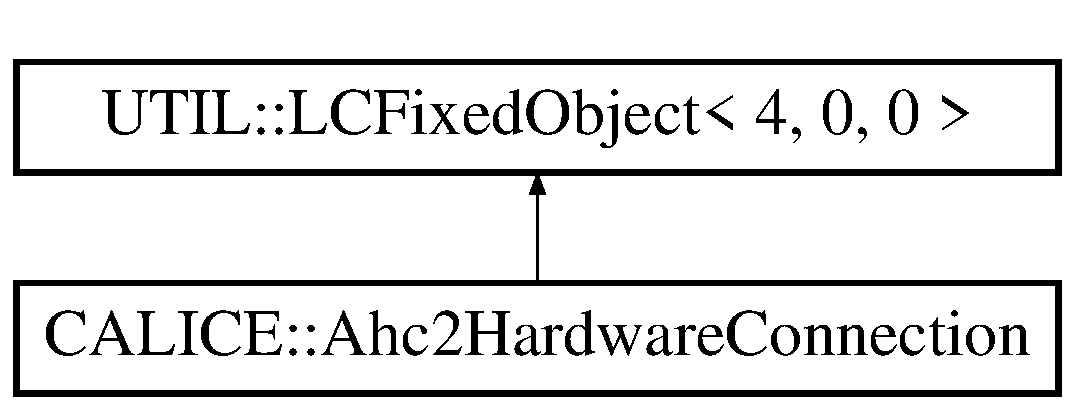
\includegraphics[height=2.000000cm]{classCALICE_1_1Ahc2HardwareConnection}
\end{center}
\end{figure}
\subsection*{Public Member Functions}
\begin{DoxyCompactItemize}
\item 
{\bf Ahc2\-Hardware\-Connection} ()\label{classCALICE_1_1Ahc2HardwareConnection_a0becd0f9301781011ab848337c3c7eab}

\begin{DoxyCompactList}\small\item\em Empty constructor. \end{DoxyCompactList}\item 
{\bf Ahc2\-Hardware\-Connection} (const int id, const int Chip, const int Module\-Number, const int Chip\-Nr)\label{classCALICE_1_1Ahc2HardwareConnection_ab19d0086bc61acb957d03a547c0ab589}

\begin{DoxyCompactList}\small\item\em Constructor with initial values. \end{DoxyCompactList}\item 
{\bf Ahc2\-Hardware\-Connection} (E\-V\-E\-N\-T\-::\-L\-C\-Object $\ast$obj)\label{classCALICE_1_1Ahc2HardwareConnection_a9c3e5db7893f4aacf68ec17cb9aeb421}

\begin{DoxyCompactList}\small\item\em Constructor from L\-C\-Object. \end{DoxyCompactList}\item 
{\bf $\sim$\-Ahc2\-Hardware\-Connection} ()\label{classCALICE_1_1Ahc2HardwareConnection_ab77e19f41adae47a8d88d10c3b171c16}

\begin{DoxyCompactList}\small\item\em Destructor. \end{DoxyCompactList}\item 
int {\bf get\-I\-D} () const \label{classCALICE_1_1Ahc2HardwareConnection_abe54d399d3d4e02c602deea3c224f8a5}

\begin{DoxyCompactList}\small\item\em Return index identifier. \end{DoxyCompactList}\item 
int {\bf get\-Chip} () const \label{classCALICE_1_1Ahc2HardwareConnection_ab7f74ef16dfe7b6a25e2c56230d0c6fc}

\begin{DoxyCompactList}\small\item\em Return the Chip\-I\-D. \end{DoxyCompactList}\item 
int {\bf get\-Module\-Number} () const \label{classCALICE_1_1Ahc2HardwareConnection_af217512dbc7bf71d2c128a9935532294}

\begin{DoxyCompactList}\small\item\em Return the Module\-Number. \end{DoxyCompactList}\item 
int {\bf get\-Chip\-Number} () const \label{classCALICE_1_1Ahc2HardwareConnection_a64b7b4c23e8d862a1d0967186022785b}

\begin{DoxyCompactList}\small\item\em Return the Chip\-Number. \end{DoxyCompactList}\item 
void {\bf set\-I\-D} (const int I\-D)\label{classCALICE_1_1Ahc2HardwareConnection_a8cf88bd1e291534c8b73a37a707e9631}

\begin{DoxyCompactList}\small\item\em set index identifier \end{DoxyCompactList}\item 
void {\bf set\-Chip} (const int Chip)\label{classCALICE_1_1Ahc2HardwareConnection_a2e3f3b9483c6564db3451cdcb0caaf88}

\begin{DoxyCompactList}\small\item\em set the Chip\-I\-D \end{DoxyCompactList}\item 
void {\bf set\-Module\-Number} (const int Module\-Number)\label{classCALICE_1_1Ahc2HardwareConnection_a65292ca8879275abf37f19fb16fd198a}

\begin{DoxyCompactList}\small\item\em set the Module\-Number \end{DoxyCompactList}\item 
void {\bf set\-Chip\-Number} (const int Chip\-Number)\label{classCALICE_1_1Ahc2HardwareConnection_aeee207bd52c55f7499f8fc5cceed2720}

\begin{DoxyCompactList}\small\item\em set the Chip\-Number \end{DoxyCompactList}\item 
virtual const std\-::string {\bf get\-Type\-Name} () const \label{classCALICE_1_1Ahc2HardwareConnection_aca4aa2ddf56a2022029fbef9f28e17a2}

\begin{DoxyCompactList}\small\item\em Implementation of L\-C\-Generic\-Object\-::get\-Type\-Name. \end{DoxyCompactList}\item 
virtual const std\-::string {\bf get\-Data\-Description} () const \label{classCALICE_1_1Ahc2HardwareConnection_a08a33f99895fb19ab59d07d6e3b46e3e}

\begin{DoxyCompactList}\small\item\em Implementation of L\-C\-Generic\-Object\-::get\-Data\-Description. \end{DoxyCompactList}\end{DoxyCompactItemize}


\subsection{Detailed Description}
Class to store int values for Hardware\-Connection plus integer cell index in L\-C\-I\-O. 

This class provides an interface to store four numbers inside an L\-C\-I\-O object\-:
\begin{DoxyItemize}
\item an integer identifier, e.\-g. the index of a calorimeter cell
\item a 1st int value, Chip\-I\-D
\item a 2nd int value, Module\-Number
\item a 3rd int value, Chip\-Number
\end{DoxyItemize}

This class is used in Ahc2\-Calibrate\-Processor to get Module\-Number and Chip\-Number from Hardware information

\begin{DoxyAuthor}{Author}
Eldwan Brianne 
\end{DoxyAuthor}
\begin{DoxyDate}{Date}
November 2015 
\end{DoxyDate}


Definition at line 27 of file Ahc2\-Hardware\-Connection.\-hh.



The documentation for this class was generated from the following file\-:\begin{DoxyCompactItemize}
\item 
Ahc2\-Hardware\-Connection.\-hh\end{DoxyCompactItemize}

\section{C\-A\-L\-I\-C\-E\-:\-:Ahc2\-Mapper Class Reference}
\label{classCALICE_1_1Ahc2Mapper}\index{C\-A\-L\-I\-C\-E\-::\-Ahc2\-Mapper@{C\-A\-L\-I\-C\-E\-::\-Ahc2\-Mapper}}


A\-H\-C\-A\-L implementation of \doxyref{Mapper}{p.}{classCALICE_1_1Mapper} class.  




{\ttfamily \#include $<$Ahc2\-Mapper.\-hh$>$}

Inheritance diagram for C\-A\-L\-I\-C\-E\-:\-:Ahc2\-Mapper\-:\begin{figure}[H]
\begin{center}
\leavevmode
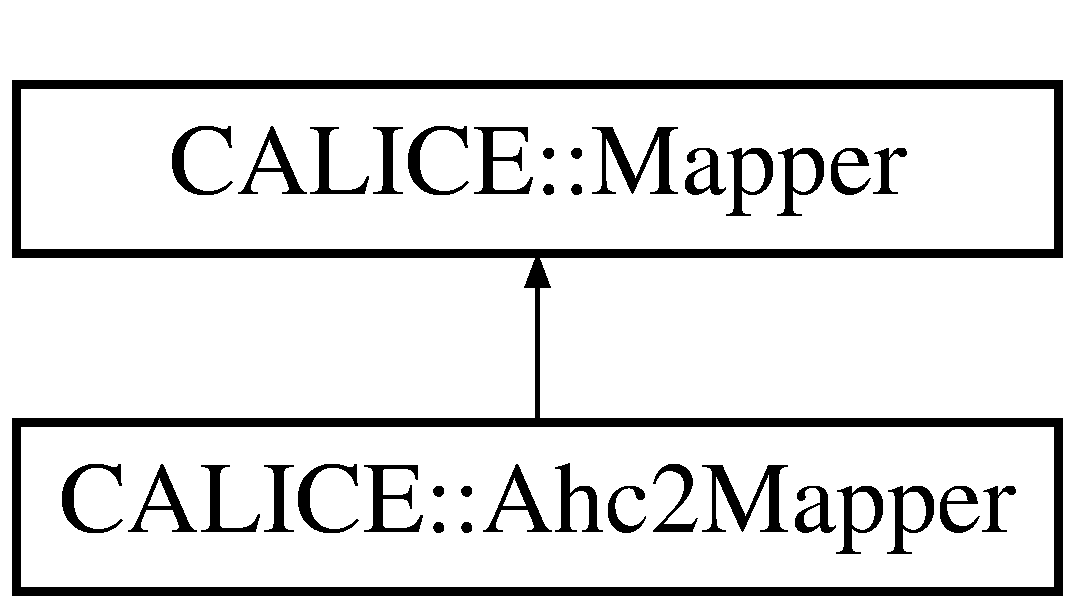
\includegraphics[height=2.000000cm]{classCALICE_1_1Ahc2Mapper}
\end{center}
\end{figure}
\subsection*{Public Member Functions}
\begin{DoxyCompactItemize}
\item 
int {\bf get\-Cell\-I\-D\-From\-Mod\-Chip\-Chan} (const unsigned int module, const unsigned int chip, const unsigned int channel) const 
\begin{DoxyCompactList}\small\item\em generate (Mokka) cell\-I\-D from module, chip, channel \end{DoxyCompactList}\item 
unsigned int {\bf get\-Module\-From\-Cell\-I\-D} (const int cell\-I\-D) const 
\begin{DoxyCompactList}\small\item\em module number from (Mokka) Cell\-I\-D \end{DoxyCompactList}\item 
unsigned int {\bf get\-Module\-From\-D\-A\-Q\-I\-D} (const int D\-A\-Qchannel) const 
\begin{DoxyCompactList}\small\item\em module number from D\-A\-Q channel I\-D \end{DoxyCompactList}\item 
unsigned int {\bf get\-Module} (const unsigned int crate, const unsigned int slot, const unsigned int fe) const 
\begin{DoxyCompactList}\small\item\em module number from triple crate, slot, fe \end{DoxyCompactList}\item 
unsigned int {\bf get\-Module} (const unsigned int k) const 
\begin{DoxyCompactList}\small\item\em module number from K \end{DoxyCompactList}\item 
unsigned int {\bf get\-Module\-From\-Cell\-I\-D} (const int cell\-I\-D, bool \&valid) const 
\begin{DoxyCompactList}\small\item\em get module (number) in which this cell is included from (Mokka) cell\-I\-D \end{DoxyCompactList}\item 
unsigned int {\bf get\-Module\-From\-D\-A\-Q\-I\-D} (const int D\-A\-Qchannel, bool \&valid) const 
\begin{DoxyCompactList}\small\item\em get module (number) in which this (D\-A\-Q) channel is included \end{DoxyCompactList}\item 
unsigned int {\bf get\-Module\-From\-Module\-I\-D} (const int module\-I\-D, bool \&valid) const 
\begin{DoxyCompactList}\small\item\em get module (number) from this (module) channel I\-D \end{DoxyCompactList}\item 
unsigned int {\bf get\-Chip\-From\-Cell\-I\-D} (const int cell\-I\-D) const 
\begin{DoxyCompactList}\small\item\em chip number from (Mokka) Cell\-I\-D \end{DoxyCompactList}\item 
unsigned int {\bf get\-Chip} (const unsigned int i, const unsigned int j, const unsigned int k) const 
\begin{DoxyCompactList}\small\item\em chip number from triple I, J, K \end{DoxyCompactList}\item 
unsigned int {\bf get\-Chan\-From\-Cell\-I\-D} (const int cell\-I\-D) const 
\begin{DoxyCompactList}\small\item\em channel number from (Mokka) Cell\-I\-D \end{DoxyCompactList}\item 
unsigned int {\bf get\-Chan} (const unsigned int i, const unsigned int j, const unsigned int k) const 
\begin{DoxyCompactList}\small\item\em chip number from triple I, J, K \end{DoxyCompactList}\item 
unsigned int {\bf get\-Crate\-From\-Cell\-I\-D} (const int cell\-I\-D) const 
\begin{DoxyCompactList}\small\item\em crate number from (Mokka) Cell\-I\-D \end{DoxyCompactList}\item 
unsigned int {\bf get\-Crate\-From\-Module\-I\-D} (const int module\-I\-D) const 
\begin{DoxyCompactList}\small\item\em crate number from Module cell I\-D \end{DoxyCompactList}\item 
unsigned int {\bf get\-Crate} (const unsigned int module) const 
\begin{DoxyCompactList}\small\item\em crate number from module number \end{DoxyCompactList}\item 
unsigned int {\bf get\-Slot\-From\-Cell\-I\-D} (const int cell\-I\-D) const 
\begin{DoxyCompactList}\small\item\em slot number from (Mokka) Cell\-I\-D \end{DoxyCompactList}\item 
unsigned int {\bf get\-Slot\-From\-Module\-I\-D} (const int module\-I\-D) const 
\begin{DoxyCompactList}\small\item\em slot number from Module cell I\-D \end{DoxyCompactList}\item 
unsigned int {\bf get\-Slot} (const unsigned int module) const 
\begin{DoxyCompactList}\small\item\em slot number from module number \end{DoxyCompactList}\item 
unsigned int {\bf get\-Fe\-From\-Cell\-I\-D} (const int cell\-I\-D) const 
\begin{DoxyCompactList}\small\item\em front end number from (Mokka) Cell\-I\-D \end{DoxyCompactList}\item 
unsigned int {\bf get\-Fe\-From\-Module\-I\-D} (const int module\-I\-D) const 
\begin{DoxyCompactList}\small\item\em front end number from Module cell I\-D \end{DoxyCompactList}\item 
unsigned int {\bf get\-Fe} (const unsigned int module) const 
\begin{DoxyCompactList}\small\item\em front end number from module number \end{DoxyCompactList}\item 
unsigned int {\bf get\-I\-From\-Module\-I\-D} (const int module\-I\-D) const 
\begin{DoxyCompactList}\small\item\em I of (Mokka) cell\-I\-D. \end{DoxyCompactList}\item 
unsigned int {\bf get\-I\-From\-D\-A\-Q\-I\-D} (const int D\-A\-Qchannel) const 
\begin{DoxyCompactList}\small\item\em I of (Mokka) cell\-I\-D. \end{DoxyCompactList}\item 
unsigned int {\bf get\-I} (const unsigned int module, const unsigned int chip, const unsigned int chan) const 
\begin{DoxyCompactList}\small\item\em I of (Mokka) cell\-I\-D. \end{DoxyCompactList}\item 
unsigned int {\bf get\-J\-From\-Module\-I\-D} (const int module\-I\-D) const 
\begin{DoxyCompactList}\small\item\em J of (Mokka) cell\-I\-D. \end{DoxyCompactList}\item 
unsigned int {\bf get\-J\-From\-D\-A\-Q\-I\-D} (const int D\-A\-Qchannel) const 
\begin{DoxyCompactList}\small\item\em J of (Mokka) cell\-I\-D. \end{DoxyCompactList}\item 
unsigned int {\bf get\-J} (const unsigned int module, const unsigned chip, const unsigned chan) const 
\begin{DoxyCompactList}\small\item\em J of (Mokka) cell\-I\-D. \end{DoxyCompactList}\item 
unsigned int {\bf get\-K\-From\-Module\-I\-D} (const int module\-I\-D) const 
\begin{DoxyCompactList}\small\item\em K of (Mokka) cell\-I\-D. \end{DoxyCompactList}\item 
unsigned int {\bf get\-K\-From\-D\-A\-Q\-I\-D} (const int D\-A\-Qchannel) const 
\begin{DoxyCompactList}\small\item\em K of (Mokka) cell\-I\-D. \end{DoxyCompactList}\item 
unsigned int {\bf get\-K} (const unsigned int module) const 
\begin{DoxyCompactList}\small\item\em K of (Mokka) cell\-I\-D. \end{DoxyCompactList}\item 
unsigned int {\bf get\-I\-Size\-From\-Cell\-I\-D} (const int cell\-I\-D) const 
\begin{DoxyCompactList}\small\item\em get cell size in I direction of (Mokka) Cell\-I\-D coordinate \end{DoxyCompactList}\item 
unsigned int {\bf get\-I\-Size\-From\-Module\-I\-D} (const int module\-I\-D) const 
\begin{DoxyCompactList}\small\item\em get cell size in I direction of (Mokka) Cell\-I\-D coordinate \end{DoxyCompactList}\item 
unsigned int {\bf get\-I\-Size\-From\-D\-A\-Q\-I\-D} (const int D\-A\-Qchannel) const 
\begin{DoxyCompactList}\small\item\em get cell size in I direction of (Mokka) Cell\-I\-D coordinate \end{DoxyCompactList}\item 
unsigned int {\bf get\-I\-Size\-From\-I\-J\-K} (const unsigned int i, const unsigned int j, const unsigned int k) const 
\begin{DoxyCompactList}\small\item\em get cell size in I direction of (Mokka) Cell\-I\-D coordinate \end{DoxyCompactList}\item 
unsigned int {\bf get\-I\-Size} (const unsigned int module, const unsigned int chip, const unsigned int chan) const 
\begin{DoxyCompactList}\small\item\em get cell size in I direction of (Mokka) Cell\-I\-D coordinate \end{DoxyCompactList}\item 
unsigned int {\bf get\-J\-Size\-From\-Cell\-I\-D} (const int cell\-I\-D) const 
\begin{DoxyCompactList}\small\item\em get cell size in J direction of (Mokka) Cell\-I\-D coordinate \end{DoxyCompactList}\item 
unsigned int {\bf get\-J\-Size\-From\-Module\-I\-D} (const int module\-I\-D) const 
\begin{DoxyCompactList}\small\item\em get cell size in J direction of (Mokka) Cell\-I\-D coordinate \end{DoxyCompactList}\item 
unsigned int {\bf get\-J\-Size\-From\-D\-A\-Q\-I\-D} (const int D\-A\-Qchannel) const 
\begin{DoxyCompactList}\small\item\em get cell size in J direction of (Mokka) Cell\-I\-D coordinate \end{DoxyCompactList}\item 
unsigned int {\bf get\-J\-Size\-From\-I\-J\-K} (const unsigned int i, const unsigned int j, const unsigned int k) const 
\begin{DoxyCompactList}\small\item\em get cell size in J direction of (Mokka) Cell\-I\-D coordinate \end{DoxyCompactList}\item 
unsigned int {\bf get\-J\-Size} (const unsigned int module, const unsigned int chip, const unsigned int chan) const 
\begin{DoxyCompactList}\small\item\em get cell size in J direction of (Mokka) Cell\-I\-D coordinate \end{DoxyCompactList}\item 
int {\bf get\-True\-Cell\-I\-D} (const int virtual\-Cell\-Index) const 
\begin{DoxyCompactList}\small\item\em return identifying index of cell \end{DoxyCompactList}\item 
int {\bf get\-True\-Cell\-I\-D} (const unsigned int i, const unsigned int j, const unsigned int k) const 
\begin{DoxyCompactList}\small\item\em return identifying index of cell \end{DoxyCompactList}\item 
unsigned int {\bf get\-True\-I\-From\-Cell\-I\-D} (const int virtual\-Cell\-I\-D) const 
\begin{DoxyCompactList}\small\item\em return I of identifying index of cell \end{DoxyCompactList}\item 
unsigned int {\bf get\-True\-I\-From\-I\-J\-K} (const unsigned int i, const unsigned int j, const unsigned int k) const 
\begin{DoxyCompactList}\small\item\em return I of identifying index of cell \end{DoxyCompactList}\item 
unsigned int {\bf get\-True\-I} (const unsigned int module, const unsigned int i, const unsigned int j) const 
\begin{DoxyCompactList}\small\item\em return I of identifying index of cell \end{DoxyCompactList}\item 
unsigned int {\bf get\-True\-J\-From\-Cell\-I\-D} (const int virtual\-Cell\-I\-D) const 
\begin{DoxyCompactList}\small\item\em return J of identifying index of cell \end{DoxyCompactList}\item 
unsigned int {\bf get\-True\-J\-From\-I\-J\-K} (const unsigned int i, const unsigned int j, const unsigned int k) const 
\begin{DoxyCompactList}\small\item\em return J of identifying index of cell \end{DoxyCompactList}\item 
unsigned int {\bf get\-True\-J} (const unsigned int module, const unsigned int i, const unsigned int j) const 
\begin{DoxyCompactList}\small\item\em return J of identifying index of cell \end{DoxyCompactList}\item 
unsigned int {\bf get\-Max\-Module} () const 
\begin{DoxyCompactList}\small\item\em return maximum module number \end{DoxyCompactList}\item 
unsigned int {\bf get\-Max\-Chip} () const 
\begin{DoxyCompactList}\small\item\em return maximum chip number \end{DoxyCompactList}\item 
unsigned int {\bf get\-Max\-Channel} () const 
\begin{DoxyCompactList}\small\item\em return maximum channel number \end{DoxyCompactList}\item 
unsigned int {\bf get\-Max\-I} () const 
\begin{DoxyCompactList}\small\item\em return maximum I index \end{DoxyCompactList}\item 
unsigned int {\bf get\-Max\-J} () const 
\begin{DoxyCompactList}\small\item\em return maximum J index \end{DoxyCompactList}\item 
unsigned int {\bf get\-Max\-K} () const 
\begin{DoxyCompactList}\small\item\em return maximum K index \end{DoxyCompactList}\item 
void {\bf fill} (const lcio\-::\-L\-C\-Collection $\ast$module\-Description\-Col, const lcio\-::\-L\-C\-Collection $\ast$module\-Connection\-Col)
\begin{DoxyCompactList}\small\item\em fills all necessary mapping information \end{DoxyCompactList}\item 
void {\bf update\-Connections} (const lcio\-::\-L\-C\-Collection $\ast$module\-Connection\-Col)
\begin{DoxyCompactList}\small\item\em updates the mapping information in the class (possible after first fill only) \end{DoxyCompactList}\item 
void {\bf print} (std\-::ostream \&ostream) const 
\begin{DoxyCompactList}\small\item\em print current data contents \end{DoxyCompactList}\item 
void {\bf print\-Stats} (std\-::ostream \&ostream) const 
\begin{DoxyCompactList}\small\item\em print summary of current data contents \end{DoxyCompactList}\end{DoxyCompactItemize}
\subsection*{Protected Member Functions}
\begin{DoxyCompactItemize}
\item 
unsigned int {\bf get\-Index\-By\-Cell\-I\-D} (const int cell\-I\-D) const 
\begin{DoxyCompactList}\small\item\em get a compact index for storing data in vectors \end{DoxyCompactList}\item 
unsigned int {\bf get\-Index\-By\-D\-A\-Q\-I\-D} (const int I\-D) const 
\begin{DoxyCompactList}\small\item\em get a compact index for storing data in vectors \end{DoxyCompactList}\item 
unsigned int {\bf get\-Index\-By\-Module\-I\-D} (const int I\-D) const 
\begin{DoxyCompactList}\small\item\em get a compact index for storing data in vectors \end{DoxyCompactList}\item 
unsigned int {\bf get\-Max\-Index} () const 
\begin{DoxyCompactList}\small\item\em get the maximum value of the compact index for storing data in vectors \end{DoxyCompactList}\item 
int {\bf get\-Cell\-I\-D\-Of\-Index} (unsigned int index) const 
\begin{DoxyCompactList}\small\item\em get the cell I\-D of a certain compact index \end{DoxyCompactList}\end{DoxyCompactItemize}
\subsection*{Private Types}
\begin{DoxyCompactItemize}
\item 
typedef std\-::map$<$ unsigned int, \\*
unsigned int $>$ {\bfseries index\-Map\-\_\-t}\label{classCALICE_1_1Ahc2Mapper_a8fa8a41634f1e55f647a1e4ccb187241}

\end{DoxyCompactItemize}
\subsection*{Private Member Functions}
\begin{DoxyCompactItemize}
\item 
bool {\bfseries valid} (const unsigned int index, const std\-::vector$<$ bool $>$ \&available\-Vec) const \label{classCALICE_1_1Ahc2Mapper_a5779fb1d18bd6941001422b70172c479}

\item 
bool {\bfseries valid} (const unsigned int index, const index\-Map\-\_\-t \&index\-Map) const \label{classCALICE_1_1Ahc2Mapper_a5ec129a4b5eb89571fac8f991e920c75}

\item 
unsigned int {\bfseries get\-Module\-Type\-Index} (const unsigned int module) const \label{classCALICE_1_1Ahc2Mapper_a7ec97081a91af002c0619e18d4508d0e}

\item 
unsigned int {\bfseries get\-Index\-Module\-Connection} (const unsigned int crate, const unsigned int slot, const unsigned int fe) const \label{classCALICE_1_1Ahc2Mapper_a37ed156f74c66d9e2339af8a4deb75d2}

\item 
unsigned int {\bfseries get\-Crate\-From\-Module\-Connection\-Index} (const unsigned int index) const \label{classCALICE_1_1Ahc2Mapper_a6a2c1f1d27a46594fa97f38360feb671}

\item 
unsigned int {\bfseries get\-Slot\-From\-Module\-Connection\-Index} (const unsigned int index) const \label{classCALICE_1_1Ahc2Mapper_abffdd8c1ca5dec03681485a3e2eeab0f}

\item 
unsigned int {\bfseries get\-Fe\-From\-Module\-Connection\-Index} (const unsigned int index) const \label{classCALICE_1_1Ahc2Mapper_aeb00ed3940d028aa4ddb3a0758ca24e9}

\item 
unsigned int {\bfseries get\-Compact\-Index} (const unsigned int module, const unsigned int chip, const unsigned int chan) const \label{classCALICE_1_1Ahc2Mapper_aed4b0468a0b060f49c68c5367ecd413a}

\item 
unsigned int {\bfseries get\-Compact\-Index} (const unsigned int module, const unsigned int chan\-Index) const \label{classCALICE_1_1Ahc2Mapper_a9c60175d4812ec36d5081c4d2d312b21}

\item 
unsigned int {\bfseries get\-Module\-From\-Compact\-Index} (const unsigned int index) const \label{classCALICE_1_1Ahc2Mapper_a1a4fbd3f35e9b55f42245da70868f97f}

\item 
unsigned int {\bfseries get\-Chip\-From\-Compact\-Index} (const unsigned int index) const \label{classCALICE_1_1Ahc2Mapper_a60e7057cb5a5920ade2cf524798889c7}

\item 
unsigned int {\bfseries get\-Chan\-From\-Compact\-Index} (const unsigned int index) const \label{classCALICE_1_1Ahc2Mapper_a2b6d7259a99f3d9b01180ca7954f824d}

\item 
unsigned int {\bfseries get\-Module\-From\-Index} (const unsigned int index, bool \&valid) const \label{classCALICE_1_1Ahc2Mapper_ace765f2bcabc77635c0dfc6f0ccfadf3}

\item 
unsigned int {\bfseries get\-Index\-Chan} (const unsigned int chip, const unsigned int chan) const \label{classCALICE_1_1Ahc2Mapper_aa4a115917ac81d3f5035e333587497c8}

\item 
unsigned int {\bfseries get\-Chip\-From\-Chan\-Index} (const unsigned int index) const \label{classCALICE_1_1Ahc2Mapper_a32ad181b781e10c534bb6bc58b462408}

\item 
unsigned int {\bfseries get\-Chan\-From\-Chan\-Index} (const unsigned int index) const \label{classCALICE_1_1Ahc2Mapper_a1ccc952c8b8e56d59a91782845cf9002}

\item 
unsigned int {\bfseries get\-Index\-I\-J} (const unsigned int i, const unsigned int j) const \label{classCALICE_1_1Ahc2Mapper_acf9ff33c6aa73b1e7d423064dbf47200}

\item 
unsigned int {\bfseries get\-I\-From\-I\-J\-Index} (const unsigned int index) const \label{classCALICE_1_1Ahc2Mapper_a0afed8a479def3e27f9277647f8fc3a0}

\item 
unsigned int {\bfseries get\-J\-From\-I\-J\-Index} (const unsigned int index) const \label{classCALICE_1_1Ahc2Mapper_a7f0ca41dc38ec81d8772fbf32c276164}

\item 
void {\bfseries clear\-Crate} ()\label{classCALICE_1_1Ahc2Mapper_a0dda73f3d42bed14be0bb9a0ea80b9f0}

\item 
void {\bfseries clear\-Slot} ()\label{classCALICE_1_1Ahc2Mapper_a2edaf45359d58bc56ac4dec0184c8207}

\item 
void {\bfseries clear\-Module\-Type} ()\label{classCALICE_1_1Ahc2Mapper_a313a204a51d33156ed7c07cc94eae746}

\item 
{\footnotesize template$<$class T $>$ }\\void {\bfseries init\-To\-Size} (std\-::vector$<$ T $>$ \&vec, const unsigned int size, const T init\-Value)\label{classCALICE_1_1Ahc2Mapper_a3a26a6a5128b44f2af0ffed3e23666cd}

\item 
void {\bfseries init\-To\-Size} (std\-::vector$<$ bool $>$ \&vec, const unsigned int size)\label{classCALICE_1_1Ahc2Mapper_a79a2bcd1def96a4108ef9df7fad2fce3}

\item 
void {\bfseries init\-To\-Size} (std\-::vector$<$ unsigned int $>$ \&data\-Vec, std\-::vector$<$ bool $>$ \&available\-Vec, const unsigned int size)\label{classCALICE_1_1Ahc2Mapper_a6d251a4da1b1132649bcb66d07e8b11d}

\item 
void {\bfseries init\-Fe} (const unsigned int max\-Fe=0)\label{classCALICE_1_1Ahc2Mapper_a58cf44c88b4ec56fed43d7bfec376051}

\item 
void {\bfseries init\-Module} (const unsigned int max\-Mod=0)\label{classCALICE_1_1Ahc2Mapper_a2e16109eb2c7730176d24534f383f097}

\item 
void {\bfseries init\-K} (const unsigned int max\-K=0)\label{classCALICE_1_1Ahc2Mapper_a4ec9ada4c15e3f01168dba3d0fd6c5eb}

\item 
void {\bfseries init\-I\-J\-Chip\-Channel} (const unsigned int max\-I=0, const unsigned int max\-J=0, const unsigned int max\-Chip=0, const unsigned int max\-Chan=0)\label{classCALICE_1_1Ahc2Mapper_aefb4e5f8d40b42f700b660a5a7107c70}

\item 
void {\bfseries clear} ()\label{classCALICE_1_1Ahc2Mapper_a1b0220e482aa59da0a2cf4024e94af47}

\item 
void {\bfseries register\-Crate} (const unsigned int crate)\label{classCALICE_1_1Ahc2Mapper_afe1d35db8e01e9b468c1c99447324239}

\item 
bool {\bfseries crate\-Available} (const unsigned int crate) const \label{classCALICE_1_1Ahc2Mapper_a8e5e8e440475134ba0c57d27f2297444}

\item 
void {\bfseries register\-Slot} (const unsigned int slot)\label{classCALICE_1_1Ahc2Mapper_a3fb5cfe4d8fa3344af19490d8023c4d7}

\item 
bool {\bfseries slot\-Available} (const unsigned int slot) const \label{classCALICE_1_1Ahc2Mapper_a31f0e0e105fe686d5f8e0ee26f84aaa4}

\item 
void {\bfseries register\-Module\-Type} (const unsigned int module\-Type\-Name)\label{classCALICE_1_1Ahc2Mapper_a27be6b81ee87fc5fca72229f6166e625}

\item 
bool {\bfseries module\-Type\-Available} (const unsigned int module\-Type\-Name) const \label{classCALICE_1_1Ahc2Mapper_ae730f5461710d7c35dbe78e82624dd5f}

\item 
unsigned int {\bfseries count\-Available} (const std\-::vector$<$ bool $>$ \&vec) const \label{classCALICE_1_1Ahc2Mapper_a82bfdf21dd843f02ea5be78a049a9007}

\item 
void {\bfseries set\-Module\-Crate\-Slot\-Fe} (const unsigned int module, const unsigned int crate, const unsigned int slot, const unsigned int fe)\label{classCALICE_1_1Ahc2Mapper_a8bc794db76e3c327e2e41200545792af}

\item 
void {\bfseries set\-Module\-Type} (const unsigned int module, const unsigned int type\-Name)\label{classCALICE_1_1Ahc2Mapper_ad704f5baff47dbdbf1dd06fd6925ec55}

\item 
void {\bfseries set\-Module\-K} (const unsigned int module, const unsigned int K)\label{classCALICE_1_1Ahc2Mapper_a816a00ce81fdd50034fbc72d09369bfb}

\item 
void {\bfseries set\-Module\-Type\-I\-J\-Chip\-Channel} (const unsigned int module\-Type\-Name, const unsigned int I, const unsigned int J, const unsigned int size\-I, const unsigned int size\-J, const unsigned int chip, const unsigned int channel)\label{classCALICE_1_1Ahc2Mapper_a7a07350fa9dd31920670adb2a3c8bdbb}

\item 
void {\bf fill\-Module\-Connection} (const lcio\-::\-L\-C\-Collection $\ast$col)
\begin{DoxyCompactList}\small\item\em sets the mapping information in the class, call after fill\-Module\-Description \end{DoxyCompactList}\item 
void {\bf fill\-Module\-Description} (const lcio\-::\-L\-C\-Collection $\ast$col)
\begin{DoxyCompactList}\small\item\em sets the module layout information in the class, module connection information will be invalidated \end{DoxyCompactList}\item 
void {\bfseries get\-Chip\-Channel\-For\-Module\-Description\-I\-D} (const unsigned int id, const unsigned int module\-Type, int \&I, int \&J) const \label{classCALICE_1_1Ahc2Mapper_a1bf9c089f6257c21f4272a00c3f65b71}

\item 
unsigned int {\bfseries get\-Combined\-Module\-Type} (const unsigned int module\-Type) const \label{classCALICE_1_1Ahc2Mapper_ab9e334091b3dd2181be96b100af757e8}

\item 
int {\bfseries correct\-Cell\-Index} (const unsigned int module\-Type, const int cell\-Index) const \label{classCALICE_1_1Ahc2Mapper_a78870e67ecf420619165292b00771753}

\item 
const std\-::string {\bfseries print\-If\-Available} (bool available, unsigned int value) const \label{classCALICE_1_1Ahc2Mapper_aa75249c8c6fd4c48a76f41d3022957f7}

\end{DoxyCompactItemize}
\subsection*{Private Attributes}
\begin{DoxyCompactItemize}
\item 
unsigned int {\bfseries \-\_\-n\-Chan}\label{classCALICE_1_1Ahc2Mapper_a9fa2e4f1e3a71c11e358f1dc51cc5fd5}

\item 
unsigned int {\bfseries \-\_\-n\-Chip}\label{classCALICE_1_1Ahc2Mapper_a0e529c3d73a93f42e26319eef4b33d44}

\item 
unsigned int {\bfseries \-\_\-n\-Fe}\label{classCALICE_1_1Ahc2Mapper_a1686f7a7a65fdca2a348587b5ab9600d}

\item 
unsigned int {\bfseries \-\_\-n\-Slot}\label{classCALICE_1_1Ahc2Mapper_a40593547c68870acc499e76687cfb883}

\item 
unsigned int {\bfseries \-\_\-max\-Slot}\label{classCALICE_1_1Ahc2Mapper_aa58dcfea6768a674f86295b0479a7ea1}

\item 
unsigned int {\bfseries \-\_\-n\-Crate}\label{classCALICE_1_1Ahc2Mapper_a0409a71622d7feb7af789d1bed2bf502}

\item 
unsigned int {\bfseries \-\_\-n\-Mod}\label{classCALICE_1_1Ahc2Mapper_a30959038e7a47577fe830d02f5c42030}

\item 
unsigned int {\bfseries \-\_\-n\-Mod\-Type}\label{classCALICE_1_1Ahc2Mapper_a78504bc4de22b3408b8a00f705b3a866}

\item 
unsigned int {\bfseries \-\_\-n\-I}\label{classCALICE_1_1Ahc2Mapper_a6844cfc402304fc896308969b7028746}

\item 
unsigned int {\bfseries \-\_\-n\-J}\label{classCALICE_1_1Ahc2Mapper_a38b7139f1417342711f1521855cc5c06}

\item 
unsigned int {\bfseries \-\_\-n\-K}\label{classCALICE_1_1Ahc2Mapper_a6835d7c3ee234599a41f6c92c221d782}

\item 
index\-Map\-\_\-t {\bfseries \-\_\-crate\-Index}\label{classCALICE_1_1Ahc2Mapper_a72f2d3b1123afe37a965760553af31df}

\item 
std\-::vector$<$ unsigned int $>$ {\bfseries \-\_\-crate\-Number}\label{classCALICE_1_1Ahc2Mapper_a99f99ee105d7a92cad6a1b2de137051c}

\item 
std\-::vector$<$ unsigned int $>$ {\bfseries \-\_\-slot\-Index}\label{classCALICE_1_1Ahc2Mapper_abed822b374b582b73ba5eb1a1a72650e}

\item 
std\-::vector$<$ unsigned int $>$ {\bfseries \-\_\-slot\-Number}\label{classCALICE_1_1Ahc2Mapper_a09a25b93e65b8050686fbeb1a4bf4fe5}

\item 
std\-::vector$<$ bool $>$ {\bfseries \-\_\-slot\-Available}\label{classCALICE_1_1Ahc2Mapper_a2c726b690ab826d55b453818c52eb3ff}

\item 
std\-::vector$<$ bool $>$ {\bfseries \-\_\-connection\-Available}\label{classCALICE_1_1Ahc2Mapper_aa6c87b52cea16672077a07b6792b0971}

\item 
std\-::vector$<$ bool $>$ {\bfseries \-\_\-module\-Available}\label{classCALICE_1_1Ahc2Mapper_a95bdac10e6000d097c537719e24545ac}

\item 
std\-::vector$<$ unsigned int $>$ {\bfseries \-\_\-type\-Vmodule}\label{classCALICE_1_1Ahc2Mapper_a0580a43e47c99b8db25aaa5a9ac8cc5a}

\item 
std\-::vector$<$ unsigned int $>$ {\bfseries \-\_\-connection\-Vmodule}\label{classCALICE_1_1Ahc2Mapper_a2e2b5d4ee46b39d39cb5fa6cde1146b6}

\item 
std\-::vector$<$ bool $>$ {\bfseries \-\_\-connection\-Vmodule\-Available}\label{classCALICE_1_1Ahc2Mapper_a83a1e56f89237e258c3a31099f8bdbbf}

\item 
std\-::vector$<$ unsigned int $>$ {\bfseries \-\_\-module\-Vconnection}\label{classCALICE_1_1Ahc2Mapper_aedbaa5da8322fd4eccaac3fb83882766}

\item 
std\-::vector$<$ unsigned int $>$ {\bfseries \-\_\-k\-Vmodule}\label{classCALICE_1_1Ahc2Mapper_aab6dabe051d9b636830b7acba209d93e}

\item 
std\-::vector$<$ bool $>$ {\bfseries \-\_\-k\-Vmodule\-Available}\label{classCALICE_1_1Ahc2Mapper_acf9257d540b74e5ca84312e34a6c2813}

\item 
std\-::vector$<$ unsigned int $>$ {\bfseries \-\_\-module\-Vk}\label{classCALICE_1_1Ahc2Mapper_ad9d8d380bce5a616ed41e27de9d0fda4}

\item 
std\-::vector$<$ bool $>$ {\bfseries \-\_\-k\-Available}\label{classCALICE_1_1Ahc2Mapper_ae2e9161b57b9d271884aa1fdfb0299bc}

\item 
std\-::vector$<$ unsigned int $>$ {\bfseries \-\_\-module\-Type\-Name}\label{classCALICE_1_1Ahc2Mapper_a6d569495b69bb4d9dac977bb26df6135}

\item 
std\-::vector$<$ unsigned int $>$ {\bfseries \-\_\-module\-Type\-Index}\label{classCALICE_1_1Ahc2Mapper_a9861340fda5c1149dc6fbabb5132865a}

\item 
std\-::vector$<$ bool $>$ {\bfseries \-\_\-module\-Type\-Available}\label{classCALICE_1_1Ahc2Mapper_a93e90fa76f22daabcb65e598e5bfed51}

\item 
std\-::vector$<$ std\-::vector\\*
$<$ unsigned int $>$ $>$ {\bfseries \-\_\-ij\-Vchan}\label{classCALICE_1_1Ahc2Mapper_a7e7cfcfc84871aab429cae7ceb83977d}

\item 
std\-::vector$<$ std\-::vector$<$ bool $>$ $>$ {\bfseries \-\_\-chip\-Chan\-Available}\label{classCALICE_1_1Ahc2Mapper_a338e6d91a30e082dd6c9887b595bbc73}

\item 
std\-::vector$<$ std\-::vector\\*
$<$ unsigned int $>$ $>$ {\bfseries \-\_\-chan\-Vij}\label{classCALICE_1_1Ahc2Mapper_ae93966f8bbc2d7f2681c1e8165b81240}

\item 
std\-::vector$<$ std\-::vector$<$ bool $>$ $>$ {\bfseries \-\_\-ij\-Available}\label{classCALICE_1_1Ahc2Mapper_acc072178aa9b3396f9abc4e60296d6c5}

\item 
std\-::vector$<$ std\-::vector$<$ bool $>$ $>$ {\bfseries \-\_\-ij\-Secondary\-Available}\label{classCALICE_1_1Ahc2Mapper_a23243017bd70e95e3788828c408cfa78}

\item 
std\-::vector$<$ std\-::vector\\*
$<$ unsigned int $>$ $>$ {\bfseries \-\_\-size\-I\-Vchan}\label{classCALICE_1_1Ahc2Mapper_ad1e47929482e3c583cd726da48bcdb68}

\item 
std\-::vector$<$ std\-::vector\\*
$<$ unsigned int $>$ $>$ {\bfseries \-\_\-size\-J\-Vchan}\label{classCALICE_1_1Ahc2Mapper_adfab042b239b997051a6c11409dab982}

\end{DoxyCompactItemize}


\subsection{Detailed Description}
A\-H\-C\-A\-L implementation of \doxyref{Mapper}{p.}{classCALICE_1_1Mapper} class. 

\begin{DoxyParagraph}{invalid cells and exception handling}
Most functions throw a \doxyref{C\-A\-L\-I\-C\-E\-::\-Bad\-Data\-Exception}{p.}{classCALICE_1_1BadDataException} if an invalid combination or I\-D is queried. Not all invalid combinations will be detected by all commands, depending on the necessary coordinate transformations in the command. E.\-g.\-: When querying the module from a Mokka cell I\-D, only K is extracted from the I\-D. If no module exists for this K an exception is thrown. But there will be no exception thrown if K is valid but I and J belong to a channel which does not exist in this module.
\end{DoxyParagraph}
\begin{DoxyParagraph}{}
The protected get\-Index\-Functions do {\bfseries not} throw exceptions to allow a fast lookup of the index. Invalid channels are signalled with return value max\-Index+1.
\end{DoxyParagraph}
\begin{DoxyParagraph}{}
Some functions have a second version that does a full check if the I\-D is valid without throwing an exception.
\end{DoxyParagraph}
\begin{DoxyAuthor}{Author}
{\tt Shaojun.\-lu@desy.\-de} 
\end{DoxyAuthor}
\begin{DoxyVersion}{Version}
0.\-1 
\end{DoxyVersion}
\begin{DoxyDate}{Date}
May 2013 
\end{DoxyDate}


Definition at line 44 of file Ahc2\-Mapper.\-hh.



\subsection{Member Function Documentation}
\index{C\-A\-L\-I\-C\-E\-::\-Ahc2\-Mapper@{C\-A\-L\-I\-C\-E\-::\-Ahc2\-Mapper}!fill@{fill}}
\index{fill@{fill}!CALICE::Ahc2Mapper@{C\-A\-L\-I\-C\-E\-::\-Ahc2\-Mapper}}
\subsubsection[{fill}]{\setlength{\rightskip}{0pt plus 5cm}void C\-A\-L\-I\-C\-E\-::\-Ahc2\-Mapper\-::fill (
\begin{DoxyParamCaption}
\item[{const lcio\-::\-L\-C\-Collection $\ast$}]{module\-Description\-Col, }
\item[{const lcio\-::\-L\-C\-Collection $\ast$}]{module\-Connection\-Col}
\end{DoxyParamCaption}
)\hspace{0.3cm}{\ttfamily [inline]}}\label{classCALICE_1_1Ahc2Mapper_a2665c4a607dec1613e91e89bb652195e}


fills all necessary mapping information 

Module layout types are set from module\-Description (chip,channel to I,J,K \& size) Module connections are set from module\-Connection (crate, slot, fe to module)

Old settings are cleared before new are set.


\begin{DoxyParams}[1]{Parameters}
\mbox{\tt in}  & {\em module\-Description\-Col} & L\-C\-Generic\-Object collection of \doxyref{Module\-Description}{p.}{classCALICE_1_1ModuleDescription} type \\
\hline
\mbox{\tt in}  & {\em module\-Connection\-Col} & L\-C\-Generic\-Object collection of \doxyref{Module\-Connection}{p.}{classCALICE_1_1ModuleConnection} type \\
\hline
\end{DoxyParams}


Definition at line 946 of file Ahc2\-Mapper.\-hh.



References fill\-Module\-Connection(), and fill\-Module\-Description().

\index{C\-A\-L\-I\-C\-E\-::\-Ahc2\-Mapper@{C\-A\-L\-I\-C\-E\-::\-Ahc2\-Mapper}!fill\-Module\-Connection@{fill\-Module\-Connection}}
\index{fill\-Module\-Connection@{fill\-Module\-Connection}!CALICE::Ahc2Mapper@{C\-A\-L\-I\-C\-E\-::\-Ahc2\-Mapper}}
\subsubsection[{fill\-Module\-Connection}]{\setlength{\rightskip}{0pt plus 5cm}void C\-A\-L\-I\-C\-E\-::\-Ahc2\-Mapper\-::fill\-Module\-Connection (
\begin{DoxyParamCaption}
\item[{const lcio\-::\-L\-C\-Collection $\ast$}]{col}
\end{DoxyParamCaption}
)\hspace{0.3cm}{\ttfamily [private]}}\label{classCALICE_1_1Ahc2Mapper_a24e7b07d1fbac2bc225a1af08fa52d38}


sets the mapping information in the class, call after fill\-Module\-Description 

The internal mapping of modules to type and electronics connection is set.


\begin{DoxyParams}[1]{Parameters}
\mbox{\tt in}  & {\em col} & L\-C\-Generic\-Object collection of \doxyref{Module\-Connection}{p.}{classCALICE_1_1ModuleConnection} type \\
\hline
\end{DoxyParams}


Definition at line 15 of file Ahc2\-Mapper.\-cc.



References C\-A\-L\-I\-C\-E\-::\-Mapper\-::mapping\-Modified().



Referenced by fill(), and update\-Connections().

\index{C\-A\-L\-I\-C\-E\-::\-Ahc2\-Mapper@{C\-A\-L\-I\-C\-E\-::\-Ahc2\-Mapper}!fill\-Module\-Description@{fill\-Module\-Description}}
\index{fill\-Module\-Description@{fill\-Module\-Description}!CALICE::Ahc2Mapper@{C\-A\-L\-I\-C\-E\-::\-Ahc2\-Mapper}}
\subsubsection[{fill\-Module\-Description}]{\setlength{\rightskip}{0pt plus 5cm}void C\-A\-L\-I\-C\-E\-::\-Ahc2\-Mapper\-::fill\-Module\-Description (
\begin{DoxyParamCaption}
\item[{const lcio\-::\-L\-C\-Collection $\ast$}]{col}
\end{DoxyParamCaption}
)\hspace{0.3cm}{\ttfamily [private]}}\label{classCALICE_1_1Ahc2Mapper_a72a2159c191b2413a13408c2f9c24480}


sets the module layout information in the class, module connection information will be invalidated 

The internal layout of modules, like channel to I,J,K and cell sizes are set.

\begin{DoxyWarning}{Warning}
module connection information will be invalidated, fill\-Module\-Connection has to be called aftwards
\end{DoxyWarning}

\begin{DoxyParams}[1]{Parameters}
\mbox{\tt in}  & {\em col} & L\-C\-Generic\-Object collection of \doxyref{Module\-Description}{p.}{classCALICE_1_1ModuleDescription} type \\
\hline
\end{DoxyParams}


Definition at line 117 of file Ahc2\-Mapper.\-cc.



References C\-A\-L\-I\-C\-E\-::\-Cell\-Index\-::get\-Pad\-Column(), C\-A\-L\-I\-C\-E\-::\-Cell\-Index\-::get\-Pad\-Row(), and C\-A\-L\-I\-C\-E\-::\-Mapper\-::mapping\-Modified().



Referenced by fill().

\index{C\-A\-L\-I\-C\-E\-::\-Ahc2\-Mapper@{C\-A\-L\-I\-C\-E\-::\-Ahc2\-Mapper}!get\-Cell\-I\-D\-Of\-Index@{get\-Cell\-I\-D\-Of\-Index}}
\index{get\-Cell\-I\-D\-Of\-Index@{get\-Cell\-I\-D\-Of\-Index}!CALICE::Ahc2Mapper@{C\-A\-L\-I\-C\-E\-::\-Ahc2\-Mapper}}
\subsubsection[{get\-Cell\-I\-D\-Of\-Index}]{\setlength{\rightskip}{0pt plus 5cm}int C\-A\-L\-I\-C\-E\-::\-Ahc2\-Mapper\-::get\-Cell\-I\-D\-Of\-Index (
\begin{DoxyParamCaption}
\item[{unsigned int}]{index}
\end{DoxyParamCaption}
) const\hspace{0.3cm}{\ttfamily [inline]}, {\ttfamily [protected]}, {\ttfamily [virtual]}}\label{classCALICE_1_1Ahc2Mapper_aa622a971f22c254c324a817355257bdc}


get the cell I\-D of a certain compact index 

\begin{DoxyWarning}{Warning}
This cell I\-D will only contain information about I, J and K. If the encoding string contains additional fields this will have value 0.
\end{DoxyWarning}
\begin{DoxySeeAlso}{See Also}
set\-Cell\-I\-Dencoding
\end{DoxySeeAlso}
\begin{DoxyReturn}{Returns}
(Mokka) cell I\-D 
\end{DoxyReturn}


Implements {\bf C\-A\-L\-I\-C\-E\-::\-Mapper} \doxyref{}{p.}{group__CellIDgroup_ga1157f15cfe97ad035e6f6fb2fd32ce2e}.



Definition at line 1070 of file Ahc2\-Mapper.\-hh.



References C\-A\-L\-I\-C\-E\-::\-Decoder\-Set\-::get\-Cell\-I\-D(), C\-A\-L\-I\-C\-E\-::\-Mapper\-::get\-Decoder(), get\-I(), get\-J(), and get\-K().

\index{C\-A\-L\-I\-C\-E\-::\-Ahc2\-Mapper@{C\-A\-L\-I\-C\-E\-::\-Ahc2\-Mapper}!get\-Chan@{get\-Chan}}
\index{get\-Chan@{get\-Chan}!CALICE::Ahc2Mapper@{C\-A\-L\-I\-C\-E\-::\-Ahc2\-Mapper}}
\subsubsection[{get\-Chan}]{\setlength{\rightskip}{0pt plus 5cm}unsigned int C\-A\-L\-I\-C\-E\-::\-Ahc2\-Mapper\-::get\-Chan (
\begin{DoxyParamCaption}
\item[{const unsigned int}]{i, }
\item[{const unsigned int}]{j, }
\item[{const unsigned int}]{k}
\end{DoxyParamCaption}
) const\hspace{0.3cm}{\ttfamily [inline]}}\label{classCALICE_1_1Ahc2Mapper_a9e2aa9c28a73ef59895d251604c6cfbb}


chip number from triple I, J, K 


\begin{DoxyParams}[1]{Parameters}
\mbox{\tt in}  & {\em i} & I \\
\hline
\mbox{\tt in}  & {\em j} & J \\
\hline
\mbox{\tt in}  & {\em k} & K\\
\hline
\end{DoxyParams}

\begin{DoxyExceptions}{Exceptions}
{\em \doxyref{Bad\-Data\-Exception}{p.}{classCALICE_1_1BadDataException}} & if invalid channel\\
\hline
\end{DoxyExceptions}
\begin{DoxyReturn}{Returns}
channel number 
\end{DoxyReturn}


Definition at line 264 of file Ahc2\-Mapper.\-hh.



References get\-Module().



Referenced by get\-Chan\-From\-Cell\-I\-D(), get\-I\-Size\-From\-I\-J\-K(), and get\-J\-Size\-From\-I\-J\-K().

\index{C\-A\-L\-I\-C\-E\-::\-Ahc2\-Mapper@{C\-A\-L\-I\-C\-E\-::\-Ahc2\-Mapper}!get\-Chip@{get\-Chip}}
\index{get\-Chip@{get\-Chip}!CALICE::Ahc2Mapper@{C\-A\-L\-I\-C\-E\-::\-Ahc2\-Mapper}}
\subsubsection[{get\-Chip}]{\setlength{\rightskip}{0pt plus 5cm}unsigned int C\-A\-L\-I\-C\-E\-::\-Ahc2\-Mapper\-::get\-Chip (
\begin{DoxyParamCaption}
\item[{const unsigned int}]{i, }
\item[{const unsigned int}]{j, }
\item[{const unsigned int}]{k}
\end{DoxyParamCaption}
) const\hspace{0.3cm}{\ttfamily [inline]}}\label{classCALICE_1_1Ahc2Mapper_a3b4555ddb636f3a1def55d7e21248b95}


chip number from triple I, J, K 


\begin{DoxyParams}[1]{Parameters}
\mbox{\tt in}  & {\em i} & I \\
\hline
\mbox{\tt in}  & {\em j} & J \\
\hline
\mbox{\tt in}  & {\em k} & K\\
\hline
\end{DoxyParams}

\begin{DoxyExceptions}{Exceptions}
{\em \doxyref{Bad\-Data\-Exception}{p.}{classCALICE_1_1BadDataException}} & if lookup fails\\
\hline
\end{DoxyExceptions}
\begin{DoxyReturn}{Returns}
chip number 
\end{DoxyReturn}


Definition at line 228 of file Ahc2\-Mapper.\-hh.



References get\-Module().



Referenced by get\-Chip\-From\-Cell\-I\-D(), get\-I\-Size\-From\-I\-J\-K(), and get\-J\-Size\-From\-I\-J\-K().

\index{C\-A\-L\-I\-C\-E\-::\-Ahc2\-Mapper@{C\-A\-L\-I\-C\-E\-::\-Ahc2\-Mapper}!get\-Crate@{get\-Crate}}
\index{get\-Crate@{get\-Crate}!CALICE::Ahc2Mapper@{C\-A\-L\-I\-C\-E\-::\-Ahc2\-Mapper}}
\subsubsection[{get\-Crate}]{\setlength{\rightskip}{0pt plus 5cm}unsigned int C\-A\-L\-I\-C\-E\-::\-Ahc2\-Mapper\-::get\-Crate (
\begin{DoxyParamCaption}
\item[{const unsigned int}]{module}
\end{DoxyParamCaption}
) const\hspace{0.3cm}{\ttfamily [inline]}}\label{classCALICE_1_1Ahc2Mapper_a085945b3737a8a6c55a4db7c441e9808}


crate number from module number 


\begin{DoxyParams}[1]{Parameters}
\mbox{\tt in}  & {\em module} & module number\\
\hline
\end{DoxyParams}

\begin{DoxyExceptions}{Exceptions}
{\em \doxyref{Bad\-Data\-Exception}{p.}{classCALICE_1_1BadDataException}} & if lookup fails\\
\hline
\end{DoxyExceptions}
\begin{DoxyReturn}{Returns}
crate number 
\end{DoxyReturn}


Definition at line 312 of file Ahc2\-Mapper.\-hh.



Referenced by get\-Crate\-From\-Cell\-I\-D(), get\-Crate\-From\-Module\-I\-D(), and print().

\index{C\-A\-L\-I\-C\-E\-::\-Ahc2\-Mapper@{C\-A\-L\-I\-C\-E\-::\-Ahc2\-Mapper}!get\-Fe@{get\-Fe}}
\index{get\-Fe@{get\-Fe}!CALICE::Ahc2Mapper@{C\-A\-L\-I\-C\-E\-::\-Ahc2\-Mapper}}
\subsubsection[{get\-Fe}]{\setlength{\rightskip}{0pt plus 5cm}unsigned int C\-A\-L\-I\-C\-E\-::\-Ahc2\-Mapper\-::get\-Fe (
\begin{DoxyParamCaption}
\item[{const unsigned int}]{module}
\end{DoxyParamCaption}
) const\hspace{0.3cm}{\ttfamily [inline]}}\label{classCALICE_1_1Ahc2Mapper_aba331d42b7ba82dd24f2ee6843d704c4}


front end number from module number 


\begin{DoxyParams}[1]{Parameters}
\mbox{\tt in}  & {\em module} & module number\\
\hline
\end{DoxyParams}

\begin{DoxyExceptions}{Exceptions}
{\em \doxyref{Bad\-Data\-Exception}{p.}{classCALICE_1_1BadDataException}} & if lookup fails\\
\hline
\end{DoxyExceptions}
\begin{DoxyReturn}{Returns}
front end number 
\end{DoxyReturn}


Definition at line 399 of file Ahc2\-Mapper.\-hh.



Referenced by get\-Fe\-From\-Cell\-I\-D(), get\-Fe\-From\-Module\-I\-D(), and print().

\index{C\-A\-L\-I\-C\-E\-::\-Ahc2\-Mapper@{C\-A\-L\-I\-C\-E\-::\-Ahc2\-Mapper}!get\-I@{get\-I}}
\index{get\-I@{get\-I}!CALICE::Ahc2Mapper@{C\-A\-L\-I\-C\-E\-::\-Ahc2\-Mapper}}
\subsubsection[{get\-I}]{\setlength{\rightskip}{0pt plus 5cm}unsigned int C\-A\-L\-I\-C\-E\-::\-Ahc2\-Mapper\-::get\-I (
\begin{DoxyParamCaption}
\item[{const unsigned int}]{module, }
\item[{const unsigned int}]{chip, }
\item[{const unsigned int}]{chan}
\end{DoxyParamCaption}
) const\hspace{0.3cm}{\ttfamily [inline]}}\label{classCALICE_1_1Ahc2Mapper_a68be5ca889254e15dc98f8ded619d2d6}


I of (Mokka) cell\-I\-D. 


\begin{DoxyParams}[1]{Parameters}
\mbox{\tt in}  & {\em module} & module number \\
\hline
\mbox{\tt in}  & {\em chip} & chip number \\
\hline
\mbox{\tt in}  & {\em chan} & channel number\\
\hline
\end{DoxyParams}

\begin{DoxyExceptions}{Exceptions}
{\em \doxyref{Bad\-Data\-Exception}{p.}{classCALICE_1_1BadDataException}} & if lookup fails\\
\hline
\end{DoxyExceptions}
\begin{DoxyReturn}{Returns}
I 
\end{DoxyReturn}


Definition at line 444 of file Ahc2\-Mapper.\-hh.



Referenced by get\-Cell\-I\-D\-From\-Mod\-Chip\-Chan(), get\-Cell\-I\-D\-Of\-Index(), get\-I\-From\-D\-A\-Q\-I\-D(), and get\-I\-From\-Module\-I\-D().

\index{C\-A\-L\-I\-C\-E\-::\-Ahc2\-Mapper@{C\-A\-L\-I\-C\-E\-::\-Ahc2\-Mapper}!get\-Index\-By\-Cell\-I\-D@{get\-Index\-By\-Cell\-I\-D}}
\index{get\-Index\-By\-Cell\-I\-D@{get\-Index\-By\-Cell\-I\-D}!CALICE::Ahc2Mapper@{C\-A\-L\-I\-C\-E\-::\-Ahc2\-Mapper}}
\subsubsection[{get\-Index\-By\-Cell\-I\-D}]{\setlength{\rightskip}{0pt plus 5cm}unsigned int C\-A\-L\-I\-C\-E\-::\-Ahc2\-Mapper\-::get\-Index\-By\-Cell\-I\-D (
\begin{DoxyParamCaption}
\item[{const int}]{cell\-I\-D}
\end{DoxyParamCaption}
) const\hspace{0.3cm}{\ttfamily [inline]}, {\ttfamily [protected]}, {\ttfamily [virtual]}}\label{classCALICE_1_1Ahc2Mapper_aa468f8c91286f9452202e0de9dc86179}


get a compact index for storing data in vectors 


\begin{DoxyParams}[1]{Parameters}
\mbox{\tt in}  & {\em cell\-I\-D} & (Mokka) cell I\-D \\
\hline
\end{DoxyParams}
\begin{DoxyReturn}{Returns}
compact index 
\end{DoxyReturn}


Implements {\bf C\-A\-L\-I\-C\-E\-::\-Mapper} \doxyref{}{p.}{group__CellIDgroup_gaaa6d826a6990c070c769f9754d2fbb76}.



Definition at line 984 of file Ahc2\-Mapper.\-hh.



References C\-A\-L\-I\-C\-E\-::\-Mapper\-::get\-Decoder(), C\-A\-L\-I\-C\-E\-::\-Decoder\-Set\-::get\-I\-From\-Cell\-I\-D(), C\-A\-L\-I\-C\-E\-::\-Decoder\-Set\-::get\-J\-From\-Cell\-I\-D(), C\-A\-L\-I\-C\-E\-::\-Decoder\-Set\-::get\-K\-From\-Cell\-I\-D(), and get\-Max\-Index().



Referenced by get\-Module\-From\-Cell\-I\-D().

\index{C\-A\-L\-I\-C\-E\-::\-Ahc2\-Mapper@{C\-A\-L\-I\-C\-E\-::\-Ahc2\-Mapper}!get\-Index\-By\-D\-A\-Q\-I\-D@{get\-Index\-By\-D\-A\-Q\-I\-D}}
\index{get\-Index\-By\-D\-A\-Q\-I\-D@{get\-Index\-By\-D\-A\-Q\-I\-D}!CALICE::Ahc2Mapper@{C\-A\-L\-I\-C\-E\-::\-Ahc2\-Mapper}}
\subsubsection[{get\-Index\-By\-D\-A\-Q\-I\-D}]{\setlength{\rightskip}{0pt plus 5cm}unsigned int C\-A\-L\-I\-C\-E\-::\-Ahc2\-Mapper\-::get\-Index\-By\-D\-A\-Q\-I\-D (
\begin{DoxyParamCaption}
\item[{const int}]{I\-D}
\end{DoxyParamCaption}
) const\hspace{0.3cm}{\ttfamily [inline]}, {\ttfamily [protected]}, {\ttfamily [virtual]}}\label{classCALICE_1_1Ahc2Mapper_a8503c24f6eab43e134845efc48654908}


get a compact index for storing data in vectors 


\begin{DoxyParams}[1]{Parameters}
\mbox{\tt in}  & {\em I\-D} & D\-A\-Q channel I\-D \\
\hline
\end{DoxyParams}
\begin{DoxyReturn}{Returns}
compact index 
\end{DoxyReturn}


Implements {\bf C\-A\-L\-I\-C\-E\-::\-Mapper} \doxyref{}{p.}{group__DAQgroup_ga4c00b2760cd3e935bed9db2f3fd28b06}.



Definition at line 1007 of file Ahc2\-Mapper.\-hh.



References C\-A\-L\-I\-C\-E\-::\-Decoder\-Set\-::get\-Channel\-From\-D\-A\-Q\-I\-D(), C\-A\-L\-I\-C\-E\-::\-Decoder\-Set\-::get\-Chip\-From\-D\-A\-Q\-I\-D(), C\-A\-L\-I\-C\-E\-::\-Decoder\-Set\-::get\-Crate\-From\-D\-A\-Q\-I\-D(), C\-A\-L\-I\-C\-E\-::\-Mapper\-::get\-Decoder(), C\-A\-L\-I\-C\-E\-::\-Decoder\-Set\-::get\-Fe\-From\-D\-A\-Q\-I\-D(), get\-Max\-Index(), and C\-A\-L\-I\-C\-E\-::\-Decoder\-Set\-::get\-Slot\-From\-D\-A\-Q\-I\-D().



Referenced by get\-Module\-From\-D\-A\-Q\-I\-D().

\index{C\-A\-L\-I\-C\-E\-::\-Ahc2\-Mapper@{C\-A\-L\-I\-C\-E\-::\-Ahc2\-Mapper}!get\-Index\-By\-Module\-I\-D@{get\-Index\-By\-Module\-I\-D}}
\index{get\-Index\-By\-Module\-I\-D@{get\-Index\-By\-Module\-I\-D}!CALICE::Ahc2Mapper@{C\-A\-L\-I\-C\-E\-::\-Ahc2\-Mapper}}
\subsubsection[{get\-Index\-By\-Module\-I\-D}]{\setlength{\rightskip}{0pt plus 5cm}unsigned int C\-A\-L\-I\-C\-E\-::\-Ahc2\-Mapper\-::get\-Index\-By\-Module\-I\-D (
\begin{DoxyParamCaption}
\item[{const int}]{I\-D}
\end{DoxyParamCaption}
) const\hspace{0.3cm}{\ttfamily [inline]}, {\ttfamily [protected]}, {\ttfamily [virtual]}}\label{classCALICE_1_1Ahc2Mapper_a3471e5014da85986b145f08b977d2e94}


get a compact index for storing data in vectors 


\begin{DoxyParams}[1]{Parameters}
\mbox{\tt in}  & {\em I\-D} & Module channel I\-D \\
\hline
\end{DoxyParams}
\begin{DoxyReturn}{Returns}
compact index 
\end{DoxyReturn}


Implements {\bf C\-A\-L\-I\-C\-E\-::\-Mapper} \doxyref{}{p.}{group__ModuleIDgroup_gad546fcc374c9168872a957d90d62bda3}.



Definition at line 1042 of file Ahc2\-Mapper.\-hh.



References C\-A\-L\-I\-C\-E\-::\-Decoder\-Set\-::get\-Channel\-From\-Module\-I\-D(), C\-A\-L\-I\-C\-E\-::\-Decoder\-Set\-::get\-Chip\-From\-Module\-I\-D(), C\-A\-L\-I\-C\-E\-::\-Mapper\-::get\-Decoder(), get\-Max\-Index(), and C\-A\-L\-I\-C\-E\-::\-Decoder\-Set\-::get\-Module\-From\-Module\-I\-D().



Referenced by get\-Module\-From\-Module\-I\-D().

\index{C\-A\-L\-I\-C\-E\-::\-Ahc2\-Mapper@{C\-A\-L\-I\-C\-E\-::\-Ahc2\-Mapper}!get\-I\-Size@{get\-I\-Size}}
\index{get\-I\-Size@{get\-I\-Size}!CALICE::Ahc2Mapper@{C\-A\-L\-I\-C\-E\-::\-Ahc2\-Mapper}}
\subsubsection[{get\-I\-Size}]{\setlength{\rightskip}{0pt plus 5cm}unsigned int C\-A\-L\-I\-C\-E\-::\-Ahc2\-Mapper\-::get\-I\-Size (
\begin{DoxyParamCaption}
\item[{const unsigned int}]{module, }
\item[{const unsigned int}]{chip, }
\item[{const unsigned int}]{chan}
\end{DoxyParamCaption}
) const\hspace{0.3cm}{\ttfamily [inline]}}\label{classCALICE_1_1Ahc2Mapper_a52d8a9ca0d55fc87f92d339ec763b514}


get cell size in I direction of (Mokka) Cell\-I\-D coordinate 


\begin{DoxyParams}[1]{Parameters}
\mbox{\tt in}  & {\em module} & module number \\
\hline
\mbox{\tt in}  & {\em chip} & chip number \\
\hline
\mbox{\tt in}  & {\em chan} & channel number\\
\hline
\end{DoxyParams}
\begin{DoxyReturn}{Returns}
size in I
\end{DoxyReturn}

\begin{DoxyExceptions}{Exceptions}
{\em \doxyref{Bad\-Data\-Exception}{p.}{classCALICE_1_1BadDataException}} & if lookup fails \\
\hline
\end{DoxyExceptions}


Definition at line 614 of file Ahc2\-Mapper.\-hh.



Referenced by get\-I\-Size\-From\-D\-A\-Q\-I\-D(), get\-I\-Size\-From\-I\-J\-K(), and get\-I\-Size\-From\-Module\-I\-D().

\index{C\-A\-L\-I\-C\-E\-::\-Ahc2\-Mapper@{C\-A\-L\-I\-C\-E\-::\-Ahc2\-Mapper}!get\-I\-Size\-From\-I\-J\-K@{get\-I\-Size\-From\-I\-J\-K}}
\index{get\-I\-Size\-From\-I\-J\-K@{get\-I\-Size\-From\-I\-J\-K}!CALICE::Ahc2Mapper@{C\-A\-L\-I\-C\-E\-::\-Ahc2\-Mapper}}
\subsubsection[{get\-I\-Size\-From\-I\-J\-K}]{\setlength{\rightskip}{0pt plus 5cm}unsigned int C\-A\-L\-I\-C\-E\-::\-Ahc2\-Mapper\-::get\-I\-Size\-From\-I\-J\-K (
\begin{DoxyParamCaption}
\item[{const unsigned int}]{i, }
\item[{const unsigned int}]{j, }
\item[{const unsigned int}]{k}
\end{DoxyParamCaption}
) const\hspace{0.3cm}{\ttfamily [inline]}}\label{classCALICE_1_1Ahc2Mapper_acf96a7b43c787c30876d5a3b8df68a5c}


get cell size in I direction of (Mokka) Cell\-I\-D coordinate 


\begin{DoxyParams}[1]{Parameters}
\mbox{\tt in}  & {\em i} & I \\
\hline
\mbox{\tt in}  & {\em j} & J \\
\hline
\mbox{\tt in}  & {\em k} & K\\
\hline
\end{DoxyParams}
\begin{DoxyReturn}{Returns}
size in I
\end{DoxyReturn}

\begin{DoxyExceptions}{Exceptions}
{\em \doxyref{Bad\-Data\-Exception}{p.}{classCALICE_1_1BadDataException}} & if lookup fails \\
\hline
\end{DoxyExceptions}


Definition at line 600 of file Ahc2\-Mapper.\-hh.



References get\-Chan(), get\-Chip(), get\-I\-Size(), and get\-Module().



Referenced by get\-I\-Size\-From\-Cell\-I\-D().

\index{C\-A\-L\-I\-C\-E\-::\-Ahc2\-Mapper@{C\-A\-L\-I\-C\-E\-::\-Ahc2\-Mapper}!get\-J@{get\-J}}
\index{get\-J@{get\-J}!CALICE::Ahc2Mapper@{C\-A\-L\-I\-C\-E\-::\-Ahc2\-Mapper}}
\subsubsection[{get\-J}]{\setlength{\rightskip}{0pt plus 5cm}unsigned int C\-A\-L\-I\-C\-E\-::\-Ahc2\-Mapper\-::get\-J (
\begin{DoxyParamCaption}
\item[{const unsigned int}]{module, }
\item[{const unsigned}]{chip, }
\item[{const unsigned}]{chan}
\end{DoxyParamCaption}
) const\hspace{0.3cm}{\ttfamily [inline]}}\label{classCALICE_1_1Ahc2Mapper_a50f1c14d9fb052f9ec91fc7611cf86a9}


J of (Mokka) cell\-I\-D. 


\begin{DoxyParams}[1]{Parameters}
\mbox{\tt in}  & {\em module} & module number \\
\hline
\mbox{\tt in}  & {\em chip} & chip number \\
\hline
\mbox{\tt in}  & {\em chan} & channel number\\
\hline
\end{DoxyParams}

\begin{DoxyExceptions}{Exceptions}
{\em \doxyref{Bad\-Data\-Exception}{p.}{classCALICE_1_1BadDataException}} & if lookup fails\\
\hline
\end{DoxyExceptions}
\begin{DoxyReturn}{Returns}
J 
\end{DoxyReturn}


Definition at line 493 of file Ahc2\-Mapper.\-hh.



Referenced by get\-Cell\-I\-D\-From\-Mod\-Chip\-Chan(), get\-Cell\-I\-D\-Of\-Index(), get\-J\-From\-D\-A\-Q\-I\-D(), and get\-J\-From\-Module\-I\-D().

\index{C\-A\-L\-I\-C\-E\-::\-Ahc2\-Mapper@{C\-A\-L\-I\-C\-E\-::\-Ahc2\-Mapper}!get\-J\-Size@{get\-J\-Size}}
\index{get\-J\-Size@{get\-J\-Size}!CALICE::Ahc2Mapper@{C\-A\-L\-I\-C\-E\-::\-Ahc2\-Mapper}}
\subsubsection[{get\-J\-Size}]{\setlength{\rightskip}{0pt plus 5cm}unsigned int C\-A\-L\-I\-C\-E\-::\-Ahc2\-Mapper\-::get\-J\-Size (
\begin{DoxyParamCaption}
\item[{const unsigned int}]{module, }
\item[{const unsigned int}]{chip, }
\item[{const unsigned int}]{chan}
\end{DoxyParamCaption}
) const\hspace{0.3cm}{\ttfamily [inline]}}\label{classCALICE_1_1Ahc2Mapper_a2a086e94e80f98fd77ba49656a42f036}


get cell size in J direction of (Mokka) Cell\-I\-D coordinate 


\begin{DoxyParams}[1]{Parameters}
\mbox{\tt in}  & {\em module} & module number \\
\hline
\mbox{\tt in}  & {\em chip} & chip number \\
\hline
\mbox{\tt in}  & {\em chan} & channel number\\
\hline
\end{DoxyParams}
\begin{DoxyReturn}{Returns}
size in J
\end{DoxyReturn}

\begin{DoxyExceptions}{Exceptions}
{\em \doxyref{Bad\-Data\-Exception}{p.}{classCALICE_1_1BadDataException}} & if lookup fails \\
\hline
\end{DoxyExceptions}


Definition at line 692 of file Ahc2\-Mapper.\-hh.



Referenced by get\-J\-Size\-From\-D\-A\-Q\-I\-D(), get\-J\-Size\-From\-I\-J\-K(), and get\-J\-Size\-From\-Module\-I\-D().

\index{C\-A\-L\-I\-C\-E\-::\-Ahc2\-Mapper@{C\-A\-L\-I\-C\-E\-::\-Ahc2\-Mapper}!get\-J\-Size\-From\-I\-J\-K@{get\-J\-Size\-From\-I\-J\-K}}
\index{get\-J\-Size\-From\-I\-J\-K@{get\-J\-Size\-From\-I\-J\-K}!CALICE::Ahc2Mapper@{C\-A\-L\-I\-C\-E\-::\-Ahc2\-Mapper}}
\subsubsection[{get\-J\-Size\-From\-I\-J\-K}]{\setlength{\rightskip}{0pt plus 5cm}unsigned int C\-A\-L\-I\-C\-E\-::\-Ahc2\-Mapper\-::get\-J\-Size\-From\-I\-J\-K (
\begin{DoxyParamCaption}
\item[{const unsigned int}]{i, }
\item[{const unsigned int}]{j, }
\item[{const unsigned int}]{k}
\end{DoxyParamCaption}
) const\hspace{0.3cm}{\ttfamily [inline]}}\label{classCALICE_1_1Ahc2Mapper_a255332c0e41298be7325bb1a91658abb}


get cell size in J direction of (Mokka) Cell\-I\-D coordinate 


\begin{DoxyParams}[1]{Parameters}
\mbox{\tt in}  & {\em i} & I \\
\hline
\mbox{\tt in}  & {\em j} & J \\
\hline
\mbox{\tt in}  & {\em k} & K\\
\hline
\end{DoxyParams}
\begin{DoxyReturn}{Returns}
size in J
\end{DoxyReturn}

\begin{DoxyExceptions}{Exceptions}
{\em \doxyref{Bad\-Data\-Exception}{p.}{classCALICE_1_1BadDataException}} & if lookup fails \\
\hline
\end{DoxyExceptions}


Definition at line 678 of file Ahc2\-Mapper.\-hh.



References get\-Chan(), get\-Chip(), get\-J\-Size(), and get\-Module().



Referenced by get\-J\-Size\-From\-Cell\-I\-D().

\index{C\-A\-L\-I\-C\-E\-::\-Ahc2\-Mapper@{C\-A\-L\-I\-C\-E\-::\-Ahc2\-Mapper}!get\-K@{get\-K}}
\index{get\-K@{get\-K}!CALICE::Ahc2Mapper@{C\-A\-L\-I\-C\-E\-::\-Ahc2\-Mapper}}
\subsubsection[{get\-K}]{\setlength{\rightskip}{0pt plus 5cm}unsigned int C\-A\-L\-I\-C\-E\-::\-Ahc2\-Mapper\-::get\-K (
\begin{DoxyParamCaption}
\item[{const unsigned int}]{module}
\end{DoxyParamCaption}
) const\hspace{0.3cm}{\ttfamily [inline]}}\label{classCALICE_1_1Ahc2Mapper_aa246f415919db6fa4a7139f0907f3856}


K of (Mokka) cell\-I\-D. 


\begin{DoxyParams}[1]{Parameters}
\mbox{\tt in}  & {\em module} & module number\\
\hline
\end{DoxyParams}
\begin{DoxyReturn}{Returns}
K
\end{DoxyReturn}

\begin{DoxyExceptions}{Exceptions}
{\em \doxyref{Bad\-Data\-Exception}{p.}{classCALICE_1_1BadDataException}} & if lookup fails \\
\hline
\end{DoxyExceptions}


Definition at line 540 of file Ahc2\-Mapper.\-hh.



Referenced by get\-Cell\-I\-D\-From\-Mod\-Chip\-Chan(), get\-Cell\-I\-D\-Of\-Index(), get\-K\-From\-D\-A\-Q\-I\-D(), get\-K\-From\-Module\-I\-D(), and print().

\index{C\-A\-L\-I\-C\-E\-::\-Ahc2\-Mapper@{C\-A\-L\-I\-C\-E\-::\-Ahc2\-Mapper}!get\-Max\-Index@{get\-Max\-Index}}
\index{get\-Max\-Index@{get\-Max\-Index}!CALICE::Ahc2Mapper@{C\-A\-L\-I\-C\-E\-::\-Ahc2\-Mapper}}
\subsubsection[{get\-Max\-Index}]{\setlength{\rightskip}{0pt plus 5cm}unsigned int C\-A\-L\-I\-C\-E\-::\-Ahc2\-Mapper\-::get\-Max\-Index (
\begin{DoxyParamCaption}
{}
\end{DoxyParamCaption}
) const\hspace{0.3cm}{\ttfamily [inline]}, {\ttfamily [protected]}, {\ttfamily [virtual]}}\label{classCALICE_1_1Ahc2Mapper_a628441b11caa652f1d13599675b8da6d}


get the maximum value of the compact index for storing data in vectors 

\begin{DoxyReturn}{Returns}
maximum compact index 
\end{DoxyReturn}


Implements {\bf C\-A\-L\-I\-C\-E\-::\-Mapper} \doxyref{}{p.}{classCALICE_1_1Mapper_a34292aca2d87f6fc7f10094b5f7cab0e}.



Definition at line 1066 of file Ahc2\-Mapper.\-hh.



Referenced by get\-Index\-By\-Cell\-I\-D(), get\-Index\-By\-D\-A\-Q\-I\-D(), and get\-Index\-By\-Module\-I\-D().

\index{C\-A\-L\-I\-C\-E\-::\-Ahc2\-Mapper@{C\-A\-L\-I\-C\-E\-::\-Ahc2\-Mapper}!get\-Module@{get\-Module}}
\index{get\-Module@{get\-Module}!CALICE::Ahc2Mapper@{C\-A\-L\-I\-C\-E\-::\-Ahc2\-Mapper}}
\subsubsection[{get\-Module}]{\setlength{\rightskip}{0pt plus 5cm}unsigned int C\-A\-L\-I\-C\-E\-::\-Ahc2\-Mapper\-::get\-Module (
\begin{DoxyParamCaption}
\item[{const unsigned int}]{crate, }
\item[{const unsigned int}]{slot, }
\item[{const unsigned int}]{fe}
\end{DoxyParamCaption}
) const\hspace{0.3cm}{\ttfamily [inline]}}\label{classCALICE_1_1Ahc2Mapper_aed5a4c86115e9048a4cded8429f85e4e}


module number from triple crate, slot, fe 


\begin{DoxyParams}[1]{Parameters}
\mbox{\tt in}  & {\em crate} & crate number (should be 0xac) \\
\hline
\mbox{\tt in}  & {\em slot} & slot number \\
\hline
\mbox{\tt in}  & {\em fe} & fe number\\
\hline
\end{DoxyParams}
\begin{DoxyReturn}{Returns}
module number
\end{DoxyReturn}

\begin{DoxyExceptions}{Exceptions}
{\em \doxyref{Bad\-Data\-Exception}{p.}{classCALICE_1_1BadDataException}} & if lookup fails \\
\hline
\end{DoxyExceptions}


Definition at line 124 of file Ahc2\-Mapper.\-hh.



Referenced by get\-Chan(), get\-Chip(), get\-I\-Size\-From\-I\-J\-K(), get\-J\-Size\-From\-I\-J\-K(), get\-Module\-From\-Cell\-I\-D(), get\-Module\-From\-D\-A\-Q\-I\-D(), get\-True\-I\-From\-I\-J\-K(), and get\-True\-J\-From\-I\-J\-K().

\index{C\-A\-L\-I\-C\-E\-::\-Ahc2\-Mapper@{C\-A\-L\-I\-C\-E\-::\-Ahc2\-Mapper}!get\-Module@{get\-Module}}
\index{get\-Module@{get\-Module}!CALICE::Ahc2Mapper@{C\-A\-L\-I\-C\-E\-::\-Ahc2\-Mapper}}
\subsubsection[{get\-Module}]{\setlength{\rightskip}{0pt plus 5cm}unsigned int C\-A\-L\-I\-C\-E\-::\-Ahc2\-Mapper\-::get\-Module (
\begin{DoxyParamCaption}
\item[{const unsigned int}]{k}
\end{DoxyParamCaption}
) const\hspace{0.3cm}{\ttfamily [inline]}}\label{classCALICE_1_1Ahc2Mapper_a43d10d6fa909332e4744fce0986b9bc4}


module number from K 


\begin{DoxyParams}[1]{Parameters}
\mbox{\tt in}  & {\em k} & K\\
\hline
\end{DoxyParams}

\begin{DoxyExceptions}{Exceptions}
{\em \doxyref{Bad\-Data\-Exception}{p.}{classCALICE_1_1BadDataException}} & if lookup fails\\
\hline
\end{DoxyExceptions}
\begin{DoxyReturn}{Returns}
module number 
\end{DoxyReturn}


Definition at line 141 of file Ahc2\-Mapper.\-hh.



References C\-A\-L\-I\-C\-E\-::\-Decoder\-Set\-::get\-Cell\-I\-D\-Encoding(), and C\-A\-L\-I\-C\-E\-::\-Mapper\-::get\-Decoder().

\index{C\-A\-L\-I\-C\-E\-::\-Ahc2\-Mapper@{C\-A\-L\-I\-C\-E\-::\-Ahc2\-Mapper}!get\-Slot@{get\-Slot}}
\index{get\-Slot@{get\-Slot}!CALICE::Ahc2Mapper@{C\-A\-L\-I\-C\-E\-::\-Ahc2\-Mapper}}
\subsubsection[{get\-Slot}]{\setlength{\rightskip}{0pt plus 5cm}unsigned int C\-A\-L\-I\-C\-E\-::\-Ahc2\-Mapper\-::get\-Slot (
\begin{DoxyParamCaption}
\item[{const unsigned int}]{module}
\end{DoxyParamCaption}
) const\hspace{0.3cm}{\ttfamily [inline]}}\label{classCALICE_1_1Ahc2Mapper_a8efe9ffb7828059f261b6321bc57f8d1}


slot number from module number 


\begin{DoxyParams}[1]{Parameters}
\mbox{\tt in}  & {\em module} & module number\\
\hline
\end{DoxyParams}

\begin{DoxyExceptions}{Exceptions}
{\em \doxyref{Bad\-Data\-Exception}{p.}{classCALICE_1_1BadDataException}} & if lookup fails\\
\hline
\end{DoxyExceptions}
\begin{DoxyReturn}{Returns}
slot number 
\end{DoxyReturn}


Definition at line 355 of file Ahc2\-Mapper.\-hh.



Referenced by get\-Slot\-From\-Cell\-I\-D(), get\-Slot\-From\-Module\-I\-D(), and print().

\index{C\-A\-L\-I\-C\-E\-::\-Ahc2\-Mapper@{C\-A\-L\-I\-C\-E\-::\-Ahc2\-Mapper}!print@{print}}
\index{print@{print}!CALICE::Ahc2Mapper@{C\-A\-L\-I\-C\-E\-::\-Ahc2\-Mapper}}
\subsubsection[{print}]{\setlength{\rightskip}{0pt plus 5cm}void C\-A\-L\-I\-C\-E\-::\-Ahc2\-Mapper\-::print (
\begin{DoxyParamCaption}
\item[{std\-::ostream \&}]{ostream}
\end{DoxyParamCaption}
) const}\label{classCALICE_1_1Ahc2Mapper_a8aa8a195c832a6dd6884f2363a76c962}


print current data contents 

A detailed printout of the current layout is sent to the given stream.


\begin{DoxyParams}[1]{Parameters}
\mbox{\tt out}  & {\em ostream} & stream for the output \\
\hline
\end{DoxyParams}


Definition at line 297 of file Ahc2\-Mapper.\-cc.



References get\-Crate(), get\-Fe(), get\-K(), and get\-Slot().

\index{C\-A\-L\-I\-C\-E\-::\-Ahc2\-Mapper@{C\-A\-L\-I\-C\-E\-::\-Ahc2\-Mapper}!print\-Stats@{print\-Stats}}
\index{print\-Stats@{print\-Stats}!CALICE::Ahc2Mapper@{C\-A\-L\-I\-C\-E\-::\-Ahc2\-Mapper}}
\subsubsection[{print\-Stats}]{\setlength{\rightskip}{0pt plus 5cm}void C\-A\-L\-I\-C\-E\-::\-Ahc2\-Mapper\-::print\-Stats (
\begin{DoxyParamCaption}
\item[{std\-::ostream \&}]{ostream}
\end{DoxyParamCaption}
) const}\label{classCALICE_1_1Ahc2Mapper_ad8829596dc41165ed72dc2732510db77}


print summary of current data contents 

A summary of the current number of module types, modules, etc... is printed.


\begin{DoxyParams}[1]{Parameters}
\mbox{\tt out}  & {\em ostream} & stream for the output \\
\hline
\end{DoxyParams}


Definition at line 265 of file Ahc2\-Mapper.\-cc.

\index{C\-A\-L\-I\-C\-E\-::\-Ahc2\-Mapper@{C\-A\-L\-I\-C\-E\-::\-Ahc2\-Mapper}!update\-Connections@{update\-Connections}}
\index{update\-Connections@{update\-Connections}!CALICE::Ahc2Mapper@{C\-A\-L\-I\-C\-E\-::\-Ahc2\-Mapper}}
\subsubsection[{update\-Connections}]{\setlength{\rightskip}{0pt plus 5cm}void C\-A\-L\-I\-C\-E\-::\-Ahc2\-Mapper\-::update\-Connections (
\begin{DoxyParamCaption}
\item[{const lcio\-::\-L\-C\-Collection $\ast$}]{module\-Connection\-Col}
\end{DoxyParamCaption}
)\hspace{0.3cm}{\ttfamily [inline]}}\label{classCALICE_1_1Ahc2Mapper_a6c3fa67ba92476bb559224f471d93e3c}


updates the mapping information in the class (possible after first fill only) 

The internal mapping of modules to type and electronics connection is updated.


\begin{DoxyParams}[1]{Parameters}
\mbox{\tt in}  & {\em module\-Connection\-Col} & L\-C\-Generic\-Object collection of \doxyref{Module\-Connection}{p.}{classCALICE_1_1ModuleConnection} type \\
\hline
\end{DoxyParams}


Definition at line 958 of file Ahc2\-Mapper.\-hh.



References fill\-Module\-Connection().



The documentation for this class was generated from the following files\-:\begin{DoxyCompactItemize}
\item 
Ahc2\-Mapper.\-hh\item 
Ahc2\-Mapper.\-cc\end{DoxyCompactItemize}

\section{C\-A\-L\-I\-C\-E\-:\-:Ahc2\-Sat\-Corr Class Reference}
\label{classCALICE_1_1Ahc2SatCorr}\index{C\-A\-L\-I\-C\-E\-::\-Ahc2\-Sat\-Corr@{C\-A\-L\-I\-C\-E\-::\-Ahc2\-Sat\-Corr}}
\subsection*{Public Member Functions}
\begin{DoxyCompactItemize}
\item 
{\bfseries Ahc2\-Sat\-Corr} ({\bf Saturation\-Parameters} $\ast$saturation\-Parameters)\label{classCALICE_1_1Ahc2SatCorr_a552b6621c2f878725d70a1514cc50cc5}

\item 
float {\bfseries de\-Saturate} (const float saturated\-Signal) const \label{classCALICE_1_1Ahc2SatCorr_ab6c572ce1b1ed8d4faa47911fea1443a}

\item 
float {\bfseries de\-Saturated\-Error} (const float saturated\-Signal, const float saturated\-Signal\-Error) const \label{classCALICE_1_1Ahc2SatCorr_ae0ece65ff89cd1e35f841cf866f4a6db}

\item 
float {\bfseries saturate} (const float unsaturated\-Signal) const \label{classCALICE_1_1Ahc2SatCorr_a4649f57514389e648d95f13925dc395d}

\item 
float {\bfseries saturated\-Error} (const float unsaturated\-Signal, const float unsaturated\-Signal\-Error) const \label{classCALICE_1_1Ahc2SatCorr_ac099e86272cc99952a00afcf2c891e71}

\item 
float {\bfseries get\-Neff\-Pix} ()\label{classCALICE_1_1Ahc2SatCorr_a713a0e340580379a17d4aeae3948cef8}

\end{DoxyCompactItemize}
\subsection*{Private Attributes}
\begin{DoxyCompactItemize}
\item 
float {\bfseries \-\_\-eff\-Npix}\label{classCALICE_1_1Ahc2SatCorr_ac4a9b30dc0ce40a3125995cae2c293ae}

\end{DoxyCompactItemize}


\subsection{Detailed Description}


Definition at line 8 of file Ahc2\-Sat\-Corr.\-hh.



The documentation for this class was generated from the following files\-:\begin{DoxyCompactItemize}
\item 
Ahc2\-Sat\-Corr.\-hh\item 
Ahc2\-Sat\-Corr.\-cc\end{DoxyCompactItemize}

\section{C\-A\-L\-I\-C\-E\-:\-:Ahc2\-Tile\-Index Class Reference}
\label{classCALICE_1_1Ahc2TileIndex}\index{C\-A\-L\-I\-C\-E\-::\-Ahc2\-Tile\-Index@{C\-A\-L\-I\-C\-E\-::\-Ahc2\-Tile\-Index}}


Encodes/decodes hardware channel information for the Large \doxyref{C\-A\-L\-I\-C\-E}{p.}{namespaceCALICE} A\-H\-C\-A\-L prototype.  




{\ttfamily \#include $<$Ahc2\-Tile\-Index.\-hh$>$}

\subsection*{Public Member Functions}
\begin{DoxyCompactItemize}
\item 
{\bf Ahc2\-Tile\-Index} ()
\begin{DoxyCompactList}\small\item\em Empty constructor. \end{DoxyCompactList}\item 
{\bfseries Ahc2\-Tile\-Index} (std\-::string module\-Encoding\-String)\label{classCALICE_1_1Ahc2TileIndex_a741ee85e80eaeb8f8a877e59a3630c7b}

\item 
{\bf Ahc2\-Tile\-Index} (int index, std\-::string module\-Encoding\-String=\char`\"{}\char`\"{})\label{classCALICE_1_1Ahc2TileIndex_a0aef10843302b1e72b649edf7bd46b7e}

\begin{DoxyCompactList}\small\item\em Constructor from an integer for decoding. \end{DoxyCompactList}\item 
{\bf Ahc2\-Tile\-Index} (short mod, short chip, short chan, std\-::string module\-Encoding\-String=\char`\"{}\char`\"{})
\begin{DoxyCompactList}\small\item\em Constructor from the minimum set of parameters required for unique identification. \end{DoxyCompactList}\item 
{\bf Ahc2\-Tile\-Index} (short mod, short chip, short chan, short sipm, std\-::string module\-Encoding\-String=\char`\"{}\char`\"{})
\begin{DoxyCompactList}\small\item\em Constructor from the full set of parameters. \end{DoxyCompactList}\item 
{\bf $\sim$\-Ahc2\-Tile\-Index} ()\label{classCALICE_1_1Ahc2TileIndex_a28ec1fc4a510f974a25902ec2279892b}

\begin{DoxyCompactList}\small\item\em Destructor -\/ does nothing. \end{DoxyCompactList}\item 
unsigned int {\bf get\-Module} () const \label{classCALICE_1_1Ahc2TileIndex_a52d837a5b768fd5a0cdff7b7f42221f9}

\begin{DoxyCompactList}\small\item\em Decode module identifier. \end{DoxyCompactList}\item 
unsigned short {\bf get\-Module\-Type} () const \label{classCALICE_1_1Ahc2TileIndex_ab33c2b64160bb2b26e66e488e96a0ec8}

\begin{DoxyCompactList}\small\item\em Derive module type from module and chip identifier. \end{DoxyCompactList}\item 
unsigned short {\bf get\-Chip} () const \label{classCALICE_1_1Ahc2TileIndex_a85e39d362d4b4dcd4269f7fe096e4fdb}

\begin{DoxyCompactList}\small\item\em Decode A\-S\-I\-C identifier. \end{DoxyCompactList}\item 
unsigned short {\bf get\-Channel} () const \label{classCALICE_1_1Ahc2TileIndex_a0893a9e4039759fbc919617e9b04c503}

\begin{DoxyCompactList}\small\item\em Decode multiplex channel. \end{DoxyCompactList}\item 
unsigned short {\bf get\-Sipm} () const \label{classCALICE_1_1Ahc2TileIndex_ab61d3e31a46c7087f806abff9bab35ad}

\begin{DoxyCompactList}\small\item\em Decode Si\-P\-M number. \end{DoxyCompactList}\item 
unsigned int {\bf get\-Index} () const \label{classCALICE_1_1Ahc2TileIndex_a39e4a87b9bbe42b156a004134ec865b3}

\begin{DoxyCompactList}\small\item\em Return T\-H\-E index. \end{DoxyCompactList}\item 
{\bf Ahc2\-Tile\-Index} \& {\bf set\-Module\-Encoding\-String} (std\-::string module\-Encoding\-String)\label{classCALICE_1_1Ahc2TileIndex_a51686e409eaf9998c4f6a36e014a4634}

\begin{DoxyCompactList}\small\item\em set module encoding stirng \end{DoxyCompactList}\item 
{\bf Ahc2\-Tile\-Index} \& {\bfseries set\-Index} (unsigned int index)\label{classCALICE_1_1Ahc2TileIndex_a64bdbc64aea683d61fc7812bf96d551e}

\item 
{\bf Ahc2\-Tile\-Index} \& {\bf set\-Module} (short mod)\label{classCALICE_1_1Ahc2TileIndex_a48e0b7549bd93ae396c61c24933c4998}

\begin{DoxyCompactList}\small\item\em Encode module identifier. \end{DoxyCompactList}\item 
{\bf Ahc2\-Tile\-Index} \& {\bf set\-Chip} (short chip)\label{classCALICE_1_1Ahc2TileIndex_a61f601112b794116197860b4cf217aca}

\begin{DoxyCompactList}\small\item\em Encode A\-S\-I\-C identifier. \end{DoxyCompactList}\item 
{\bf Ahc2\-Tile\-Index} \& {\bf set\-Channel} (short chan)\label{classCALICE_1_1Ahc2TileIndex_a7dc32f4e96c886e608efc8bf1a48e91d}

\begin{DoxyCompactList}\small\item\em Encode multiplex channel. \end{DoxyCompactList}\item 
{\bf Ahc2\-Tile\-Index} \& {\bf set\-Sipm} (short sipm)\label{classCALICE_1_1Ahc2TileIndex_adb3ebef7ea8ff30202e9df1e657fee95}

\begin{DoxyCompactList}\small\item\em Encode Si\-P\-M number. \end{DoxyCompactList}\item 
std\-::string {\bf get\-Encoding\-String} (const unsigned int startbit)\label{classCALICE_1_1Ahc2TileIndex_a10fa7c1377ee78f298d505699dde0ba8}

\begin{DoxyCompactList}\small\item\em Return the cellid encoding string according to an lcio Bit\-Field64. \end{DoxyCompactList}\end{DoxyCompactItemize}
\subsection*{Protected Attributes}
\begin{DoxyCompactItemize}
\item 
unsigned int {\bfseries \-\_\-index}\label{classCALICE_1_1Ahc2TileIndex_a89014d6ace3fd676c9820c1f9e8a43e0}

\item 
std\-::string {\bfseries \-\_\-module\-Encoding\-String}\label{classCALICE_1_1Ahc2TileIndex_ab191565b86ed6a757e25c32e43e01cd3}

\item 
U\-T\-I\-L\-::\-Bit\-Field64 $\ast$ {\bfseries \-\_\-bf\-\_\-cell\-I\-D}\label{classCALICE_1_1Ahc2TileIndex_a898a68a95fc0abe58c6a9392115c32b0}

\end{DoxyCompactItemize}


\subsection{Detailed Description}
Encodes/decodes hardware channel information for the Large \doxyref{C\-A\-L\-I\-C\-E}{p.}{namespaceCALICE} A\-H\-C\-A\-L prototype. 

This class encodes and decodes module, chip and channel as well as the Si\-P\-M number into/from a single integer. This integer is intended to be stored in the Cell\-I\-D1 field of L\-C\-I\-O Calorimeter\-Hit objects for easy reference to and unique identification of the hardware information of reconstructed hits.

This class is adapted from the \doxyref{Hcal\-Tile\-Index.\-hh}{p.}{HcalTileIndex_8hh_source} class in order to make it flexible for different Cell\-I\-D encodings

\begin{DoxyAuthor}{Author}
Christian Graf 
\end{DoxyAuthor}
\begin{DoxyDate}{Date}
2018, Jan 
\end{DoxyDate}
\begin{DoxyVersion}{Version}
1.\-0 
\end{DoxyVersion}


Definition at line 29 of file Ahc2\-Tile\-Index.\-hh.



\subsection{Constructor \& Destructor Documentation}
\index{C\-A\-L\-I\-C\-E\-::\-Ahc2\-Tile\-Index@{C\-A\-L\-I\-C\-E\-::\-Ahc2\-Tile\-Index}!Ahc2\-Tile\-Index@{Ahc2\-Tile\-Index}}
\index{Ahc2\-Tile\-Index@{Ahc2\-Tile\-Index}!CALICE::Ahc2TileIndex@{C\-A\-L\-I\-C\-E\-::\-Ahc2\-Tile\-Index}}
\subsubsection[{Ahc2\-Tile\-Index}]{\setlength{\rightskip}{0pt plus 5cm}C\-A\-L\-I\-C\-E\-::\-Ahc2\-Tile\-Index\-::\-Ahc2\-Tile\-Index (
\begin{DoxyParamCaption}
{}
\end{DoxyParamCaption}
)\hspace{0.3cm}{\ttfamily [inline]}}\label{classCALICE_1_1Ahc2TileIndex_a0e21744b89c397cd9e94fc6e78f8c8dd}


Empty constructor. 

All parameters default to zero. 

Definition at line 33 of file Ahc2\-Tile\-Index.\-hh.



References set\-Channel(), set\-Chip(), set\-Module(), set\-Module\-Encoding\-String(), and set\-Sipm().

\index{C\-A\-L\-I\-C\-E\-::\-Ahc2\-Tile\-Index@{C\-A\-L\-I\-C\-E\-::\-Ahc2\-Tile\-Index}!Ahc2\-Tile\-Index@{Ahc2\-Tile\-Index}}
\index{Ahc2\-Tile\-Index@{Ahc2\-Tile\-Index}!CALICE::Ahc2TileIndex@{C\-A\-L\-I\-C\-E\-::\-Ahc2\-Tile\-Index}}
\subsubsection[{Ahc2\-Tile\-Index}]{\setlength{\rightskip}{0pt plus 5cm}C\-A\-L\-I\-C\-E\-::\-Ahc2\-Tile\-Index\-::\-Ahc2\-Tile\-Index (
\begin{DoxyParamCaption}
\item[{short}]{mod, }
\item[{short}]{chip, }
\item[{short}]{chan, }
\item[{std\-::string}]{module\-Encoding\-String = {\ttfamily \char`\"{}\char`\"{}}}
\end{DoxyParamCaption}
)\hspace{0.3cm}{\ttfamily [inline]}}\label{classCALICE_1_1Ahc2TileIndex_a82fbf0f8e0ff26830f90d4efcfb83c60}


Constructor from the minimum set of parameters required for unique identification. 

The Si\-P\-M number defaults to zero.


\begin{DoxyParams}{Parameters}
{\em mod} & Module identifier \\
\hline
{\em chip} & A\-S\-I\-C chip identifier \\
\hline
{\em chan} & Multiplex channel identifier \\
\hline
{\em module\-Encoding\-String} & encoding string \\
\hline
\end{DoxyParams}


Definition at line 90 of file Ahc2\-Tile\-Index.\-hh.



References set\-Channel(), set\-Chip(), set\-Module(), set\-Module\-Encoding\-String(), and set\-Sipm().

\index{C\-A\-L\-I\-C\-E\-::\-Ahc2\-Tile\-Index@{C\-A\-L\-I\-C\-E\-::\-Ahc2\-Tile\-Index}!Ahc2\-Tile\-Index@{Ahc2\-Tile\-Index}}
\index{Ahc2\-Tile\-Index@{Ahc2\-Tile\-Index}!CALICE::Ahc2TileIndex@{C\-A\-L\-I\-C\-E\-::\-Ahc2\-Tile\-Index}}
\subsubsection[{Ahc2\-Tile\-Index}]{\setlength{\rightskip}{0pt plus 5cm}C\-A\-L\-I\-C\-E\-::\-Ahc2\-Tile\-Index\-::\-Ahc2\-Tile\-Index (
\begin{DoxyParamCaption}
\item[{short}]{mod, }
\item[{short}]{chip, }
\item[{short}]{chan, }
\item[{short}]{sipm, }
\item[{std\-::string}]{module\-Encoding\-String = {\ttfamily \char`\"{}\char`\"{}}}
\end{DoxyParamCaption}
)\hspace{0.3cm}{\ttfamily [inline]}}\label{classCALICE_1_1Ahc2TileIndex_a6694fcab6ea3d79fc0254c45ba91fca6}


Constructor from the full set of parameters. 


\begin{DoxyParams}{Parameters}
{\em mod} & Module identifier \\
\hline
{\em chip} & A\-S\-I\-C chip identifier \\
\hline
{\em chan} & Multiplex channel identifier \\
\hline
{\em sipm} & Si\-P\-M identifier \\
\hline
{\em module\-Encoding\-String} & encoding string \\
\hline
\end{DoxyParams}


Definition at line 113 of file Ahc2\-Tile\-Index.\-hh.



References set\-Channel(), set\-Chip(), set\-Module(), set\-Module\-Encoding\-String(), and set\-Sipm().



The documentation for this class was generated from the following file\-:\begin{DoxyCompactItemize}
\item 
Ahc2\-Tile\-Index.\-hh\end{DoxyCompactItemize}

\section{C\-A\-L\-I\-C\-E\-:\-:Ahc\-Amplitude Class Reference}
\label{classCALICE_1_1AhcAmplitude}\index{C\-A\-L\-I\-C\-E\-::\-Ahc\-Amplitude@{C\-A\-L\-I\-C\-E\-::\-Ahc\-Amplitude}}
Inheritance diagram for C\-A\-L\-I\-C\-E\-:\-:Ahc\-Amplitude\-:\begin{figure}[H]
\begin{center}
\leavevmode
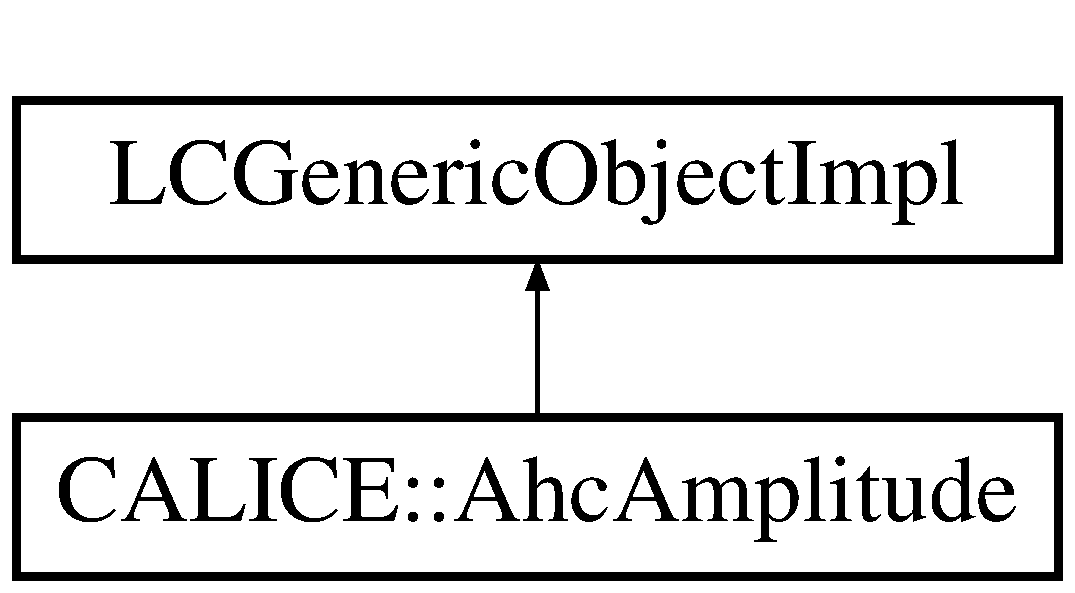
\includegraphics[height=2.000000cm]{classCALICE_1_1AhcAmplitude}
\end{center}
\end{figure}
\subsection*{Public Member Functions}
\begin{DoxyCompactItemize}
\item 
{\bf Ahc\-Amplitude} (E\-V\-E\-N\-T\-::\-L\-C\-Generic\-Object $\ast$generic\-Object)
\begin{DoxyCompactList}\small\item\em Constructor from L\-C\-Generic\-Object. \end{DoxyCompactList}\item 
{\bf Ahc\-Amplitude} ()
\begin{DoxyCompactList}\small\item\em Empty constructor. \end{DoxyCompactList}\item 
{\bf Ahc\-Amplitude} (int cell\-I\-D, float ampl\-Raw\-A\-D\-C, float ampl\-Raw\-Minus\-Pedestal\-A\-D\-C, float ampl\-Temperature\-Corr\-M\-I\-P, float ampl\-N\-O\-T\-Temperature\-Corr\-M\-I\-P, float ampl\-Ge\-V, float temperature=0)
\begin{DoxyCompactList}\small\item\em Constructor from elements. \end{DoxyCompactList}\item 
virtual {\bf $\sim$\-Ahc\-Amplitude} ()\label{classCALICE_1_1AhcAmplitude_a9098e06a99ede647985f9740bea488c9}

\begin{DoxyCompactList}\small\item\em Important for memory handling. \end{DoxyCompactList}\item 
void {\bfseries set\-Cell\-I\-D} (const int cell\-I\-D)\label{classCALICE_1_1AhcAmplitude_af30305bc770835cef1e85b52861a8d77}

\item 
const int {\bfseries get\-Cell\-I\-D} ()\label{classCALICE_1_1AhcAmplitude_a8ba74fcf68e917e51fe0815c1ff81583}

\item 
void {\bfseries set\-Ampl\-Raw\-A\-D\-C} (const float ampl\-Raw\-A\-D\-C)\label{classCALICE_1_1AhcAmplitude_a1bf9f7c2837899af1ef2df59ef94866b}

\item 
const float {\bfseries get\-Ampl\-Raw\-A\-D\-C} ()\label{classCALICE_1_1AhcAmplitude_a367d193df67de6046af58982ccb6e2ba}

\item 
void {\bfseries set\-Ampl\-Raw\-Minus\-Pedestal\-A\-D\-C} (const float ampl\-Raw\-Minus\-Pedestal\-A\-D\-C)\label{classCALICE_1_1AhcAmplitude_af248705124029b6a523b1c79b189b0bd}

\item 
const float {\bfseries get\-Ampl\-Raw\-Minus\-Pedestal\-A\-D\-C} ()\label{classCALICE_1_1AhcAmplitude_ad514eaba7b4412210f37a950b4abfe97}

\item 
void {\bfseries set\-Ampl\-Temperature\-Corr\-M\-I\-P} (const float ampl\-Temperature\-Corr\-M\-I\-P)\label{classCALICE_1_1AhcAmplitude_a0d3fd86e8d35dbbc05b3cca3f3421e75}

\item 
const float {\bfseries get\-Ampl\-Temperature\-Corr\-M\-I\-P} ()\label{classCALICE_1_1AhcAmplitude_a0b607cb3be3e999a5ac7b38dc459dd3a}

\item 
void {\bfseries set\-Ampl\-N\-O\-T\-Temperature\-Corr\-M\-I\-P} (const float ampl\-N\-O\-T\-Temperature\-Corr\-M\-I\-P)\label{classCALICE_1_1AhcAmplitude_aa26157732c7138aaee6ad7f194a3bca6}

\item 
const float {\bfseries get\-Ampl\-N\-O\-T\-Temperature\-Corr\-M\-I\-P} ()\label{classCALICE_1_1AhcAmplitude_a755d45a5e563ce40e17d312d444d99ab}

\item 
void {\bfseries set\-Ampl\-Ge\-V} (const float ampl\-Ge\-V)\label{classCALICE_1_1AhcAmplitude_a445c83887997f254e988e914eed7b670}

\item 
const float {\bfseries get\-Ampl\-Ge\-V} ()\label{classCALICE_1_1AhcAmplitude_a4289af7ccb604b8a2db0e8202efe6374}

\item 
void {\bfseries set\-Temperature} (const float temperature)\label{classCALICE_1_1AhcAmplitude_ab2872aa24017885f071a7e66181c5913}

\item 
const float {\bfseries get\-Temperature} ()\label{classCALICE_1_1AhcAmplitude_a8e820e9eb754d24fa5e6d87e2f30c00b}

\item 
const std\-::string {\bf get\-Type\-Name} () const 
\begin{DoxyCompactList}\small\item\em Implementation of the virtual method from L\-C\-Generic\-Object. \end{DoxyCompactList}\item 
const std\-::string {\bf get\-Data\-Description} () const 
\begin{DoxyCompactList}\small\item\em Implementation of the virtual method from L\-C\-Generic\-Object. \end{DoxyCompactList}\end{DoxyCompactItemize}
\subsection*{Private Types}
\begin{DoxyCompactItemize}
\item 
enum {\bfseries Ints} \{ {\bfseries k\-Cell\-I\-D}, 
{\bfseries k\-N\-Ints}
 \}
\item 
enum {\bfseries Float} \{ \\*
{\bfseries k\-Ampl\-Raw\-A\-D\-C}, 
{\bfseries k\-Ampl\-Raw\-Minus\-Pedestal\-A\-D\-C}, 
{\bfseries k\-Ampl\-Temperature\-Corr\-M\-I\-P}, 
{\bfseries k\-Ampl\-N\-O\-T\-Temperature\-Corr\-M\-I\-P}, 
\\*
{\bfseries k\-Ampl\-Ge\-V}, 
{\bfseries k\-Temperature}, 
{\bfseries k\-N\-Floats}
 \}
\item 
enum {\bfseries Doubless} \{ {\bfseries k\-N\-Doubles}
 \}
\end{DoxyCompactItemize}


\subsection{Detailed Description}


Definition at line 10 of file Ahc\-Amplitude.\-hh.



\subsection{Constructor \& Destructor Documentation}
\index{C\-A\-L\-I\-C\-E\-::\-Ahc\-Amplitude@{C\-A\-L\-I\-C\-E\-::\-Ahc\-Amplitude}!Ahc\-Amplitude@{Ahc\-Amplitude}}
\index{Ahc\-Amplitude@{Ahc\-Amplitude}!CALICE::AhcAmplitude@{C\-A\-L\-I\-C\-E\-::\-Ahc\-Amplitude}}
\subsubsection[{Ahc\-Amplitude}]{\setlength{\rightskip}{0pt plus 5cm}C\-A\-L\-I\-C\-E\-::\-Ahc\-Amplitude\-::\-Ahc\-Amplitude (
\begin{DoxyParamCaption}
\item[{E\-V\-E\-N\-T\-::\-L\-C\-Generic\-Object $\ast$}]{generic\-Object}
\end{DoxyParamCaption}
)}\label{classCALICE_1_1AhcAmplitude_ae33ff63a6cd838b59b3def113aa879cf}


Constructor from L\-C\-Generic\-Object. 

Constructor from L\-C\-Object\-: use L\-C\-Object, and do the cast from the L\-C\-Generic\-Object; this way, the users do not have to do the cast anymore. 

Definition at line 10 of file Ahc\-Amplitude.\-cc.

\index{C\-A\-L\-I\-C\-E\-::\-Ahc\-Amplitude@{C\-A\-L\-I\-C\-E\-::\-Ahc\-Amplitude}!Ahc\-Amplitude@{Ahc\-Amplitude}}
\index{Ahc\-Amplitude@{Ahc\-Amplitude}!CALICE::AhcAmplitude@{C\-A\-L\-I\-C\-E\-::\-Ahc\-Amplitude}}
\subsubsection[{Ahc\-Amplitude}]{\setlength{\rightskip}{0pt plus 5cm}C\-A\-L\-I\-C\-E\-::\-Ahc\-Amplitude\-::\-Ahc\-Amplitude (
\begin{DoxyParamCaption}
{}
\end{DoxyParamCaption}
)}\label{classCALICE_1_1AhcAmplitude_a2c64ca265f3605c0aa7418ec62f130f6}


Empty constructor. 

empty constructor 

Definition at line 38 of file Ahc\-Amplitude.\-cc.

\index{C\-A\-L\-I\-C\-E\-::\-Ahc\-Amplitude@{C\-A\-L\-I\-C\-E\-::\-Ahc\-Amplitude}!Ahc\-Amplitude@{Ahc\-Amplitude}}
\index{Ahc\-Amplitude@{Ahc\-Amplitude}!CALICE::AhcAmplitude@{C\-A\-L\-I\-C\-E\-::\-Ahc\-Amplitude}}
\subsubsection[{Ahc\-Amplitude}]{\setlength{\rightskip}{0pt plus 5cm}C\-A\-L\-I\-C\-E\-::\-Ahc\-Amplitude\-::\-Ahc\-Amplitude (
\begin{DoxyParamCaption}
\item[{int}]{cell\-I\-D, }
\item[{float}]{ampl\-Raw\-A\-D\-C, }
\item[{float}]{ampl\-Raw\-Minus\-Pedestal\-A\-D\-C, }
\item[{float}]{ampl\-Temperature\-Corr\-M\-I\-P, }
\item[{float}]{ampl\-N\-O\-T\-Temperature\-Corr\-M\-I\-P, }
\item[{float}]{ampl\-Ge\-V, }
\item[{float}]{temperature = {\ttfamily 0}}
\end{DoxyParamCaption}
)}\label{classCALICE_1_1AhcAmplitude_a5b9ac2d65b9a1e5b9a778dc656790677}


Constructor from elements. 

constructor from elements


\begin{DoxyParams}{Parameters}
{\em cell\-I\-D} & cell\-I\-D0 \\
\hline
{\em ampl\-Raw\-A\-D\-C} & raw enery, in A\-D\-C counts \\
\hline
{\em ampl\-Raw\-Minus\-Pedestal\-A\-D\-C} & pedestal subtracted raw energy, in A\-D\-C counts \\
\hline
{\em ampl\-Temperature\-Corr\-M\-I\-P} & amplitude in M\-I\-Ps, based on temperature corrected M\-I\-P \\
\hline
{\em ampl\-N\-O\-T\-Temperature\-Corr\-M\-I\-P} & amplitude in M\-I\-Ps, with M\-I\-P N\-O\-T temperature corrected \\
\hline
{\em ampl\-Ge\-V} & amplitude in Ge\-V \\
\hline
{\em temperature} & \\
\hline
\end{DoxyParams}


Definition at line 51 of file Ahc\-Amplitude.\-cc.



\subsection{Member Function Documentation}
\index{C\-A\-L\-I\-C\-E\-::\-Ahc\-Amplitude@{C\-A\-L\-I\-C\-E\-::\-Ahc\-Amplitude}!get\-Data\-Description@{get\-Data\-Description}}
\index{get\-Data\-Description@{get\-Data\-Description}!CALICE::AhcAmplitude@{C\-A\-L\-I\-C\-E\-::\-Ahc\-Amplitude}}
\subsubsection[{get\-Data\-Description}]{\setlength{\rightskip}{0pt plus 5cm}const std\-::string C\-A\-L\-I\-C\-E\-::\-Ahc\-Amplitude\-::get\-Data\-Description (
\begin{DoxyParamCaption}
{}
\end{DoxyParamCaption}
) const}\label{classCALICE_1_1AhcAmplitude_a90d5bda5b0fe75d075c0ee3f51e21154}


Implementation of the virtual method from L\-C\-Generic\-Object. 

\begin{DoxyReturn}{Returns}
data description, i.\-e description of the L\-C\-Object elements\-: \char`\"{}i\-:cell\-I\-D,f\-:ampl\-Raw\-A\-D\-C,f\-:ampl\-Raw\-Minus\-Pedestal\-A\-D\-C,f\-:ampl\-Temperature\-Corr\-M\-I\-P,f\-:ampl\-N\-O\-T\-Temperature\-Corr\-M\-I\-P,f\-:ampl\-Ge\-V,f\-:temperature\char`\"{}; 
\end{DoxyReturn}


Definition at line 156 of file Ahc\-Amplitude.\-cc.

\index{C\-A\-L\-I\-C\-E\-::\-Ahc\-Amplitude@{C\-A\-L\-I\-C\-E\-::\-Ahc\-Amplitude}!get\-Type\-Name@{get\-Type\-Name}}
\index{get\-Type\-Name@{get\-Type\-Name}!CALICE::AhcAmplitude@{C\-A\-L\-I\-C\-E\-::\-Ahc\-Amplitude}}
\subsubsection[{get\-Type\-Name}]{\setlength{\rightskip}{0pt plus 5cm}const std\-::string C\-A\-L\-I\-C\-E\-::\-Ahc\-Amplitude\-::get\-Type\-Name (
\begin{DoxyParamCaption}
{}
\end{DoxyParamCaption}
) const}\label{classCALICE_1_1AhcAmplitude_aa177cd1d27b9751a36e38775d8b439c7}


Implementation of the virtual method from L\-C\-Generic\-Object. 

\begin{DoxyReturn}{Returns}
type name, i.\-e. name of the class 
\end{DoxyReturn}


Definition at line 151 of file Ahc\-Amplitude.\-cc.



The documentation for this class was generated from the following files\-:\begin{DoxyCompactItemize}
\item 
Ahc\-Amplitude.\-hh\item 
Ahc\-Amplitude.\-cc\end{DoxyCompactItemize}

\section{C\-A\-L\-I\-C\-E\-:\-:Ahc\-Cern2010\-Temp\-Provider Class Reference}
\label{classCALICE_1_1AhcCern2010TempProvider}\index{C\-A\-L\-I\-C\-E\-::\-Ahc\-Cern2010\-Temp\-Provider@{C\-A\-L\-I\-C\-E\-::\-Ahc\-Cern2010\-Temp\-Provider}}


This is a temperature provider for the A\-H\-C\-A\-L.\-based on the studies of the temperature profiles from C\-E\-R\-N 2010 data.  




{\ttfamily \#include $<$Ahc\-Cern2010\-Temp\-Provider.\-hh$>$}

Inheritance diagram for C\-A\-L\-I\-C\-E\-:\-:Ahc\-Cern2010\-Temp\-Provider\-:\begin{figure}[H]
\begin{center}
\leavevmode
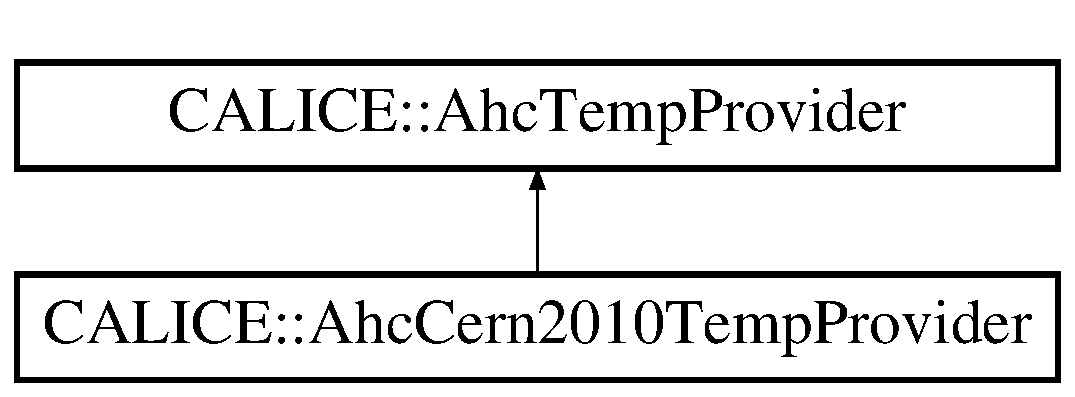
\includegraphics[height=2.000000cm]{classCALICE_1_1AhcCern2010TempProvider}
\end{center}
\end{figure}
\subsection*{Public Member Functions}
\begin{DoxyCompactItemize}
\item 
{\bfseries Ahc\-Cern2010\-Temp\-Provider} ({\bf Ahc\-Mapper} const $\ast$mapper)\label{classCALICE_1_1AhcCern2010TempProvider_a5e0bea69970f631796885bfa5e36d1ba}

\item 
void {\bfseries apply\-Correction} ()\label{classCALICE_1_1AhcCern2010TempProvider_a4df8bc703a896c74956b470211396907}

\item 
float {\bf get\-Sensor\-Temp} (int module, int sensor)
\begin{DoxyCompactList}\small\item\em Returns the temperature of the specified sensor in the given module. \end{DoxyCompactList}\item 
float {\bf get\-Cell\-Temp} (int module, int chip, int chan)
\begin{DoxyCompactList}\small\item\em Returns the temperature for the cell in the specified module connected to the given chip and channel. \end{DoxyCompactList}\item 
float {\bf get\-Cell\-Temp\-Error} (int module, int chip, int chan)
\begin{DoxyCompactList}\small\item\em Returns the error on the temperature for the cell in the specified module connected to the given chip and channel. \end{DoxyCompactList}\item 
float {\bf get\-Avg\-Temp} ()\label{classCALICE_1_1AhcCern2010TempProvider_ae70a7581cfb3f9e46fa6cf262cf4e945}

\begin{DoxyCompactList}\small\item\em Return the average calorimeter temperature. \end{DoxyCompactList}\item 
float {\bf get\-Avg\-Module\-Temp} (unsigned module)\label{classCALICE_1_1AhcCern2010TempProvider_a18085f89099caedb30b3f341487c5db8}

\begin{DoxyCompactList}\small\item\em Return the average temperature for the specified module. \end{DoxyCompactList}\item 
int {\bf get\-Sensor} (int chip, int chan)
\begin{DoxyCompactList}\small\item\em Returns the closest sensor to cell connected to chip, chan according to D\-E\-S\-Y-\/\-T\-H\-E\-S\-I\-S-\/2008-\/050. \end{DoxyCompactList}\end{DoxyCompactItemize}
\subsection*{Protected Member Functions}
\begin{DoxyCompactItemize}
\item 
void {\bfseries apply\-Correction\-For\-Unreasonable\-Sensors} (int module, int sensor)\label{classCALICE_1_1AhcCern2010TempProvider_a2cffa40eb335c8c66de5d939328215ac}

\item 
bool {\bfseries apply\-Correction\-For\-Unreasonable\-Modules} (int module, int sensor)\label{classCALICE_1_1AhcCern2010TempProvider_a36b34c7e212637d22e887a7bd8bf681c}

\end{DoxyCompactItemize}
\subsection*{Private Member Functions}
\begin{DoxyCompactItemize}
\item 
bool {\bfseries is\-Module\-Off} (int module)\label{classCALICE_1_1AhcCern2010TempProvider_a2c784e8262e279884622c9a31ef504c8}

\item 
double {\bfseries median} (float a[$\,$], int n)\label{classCALICE_1_1AhcCern2010TempProvider_aee3afaa7ee7c7ed1a16b577f92033c49}

\end{DoxyCompactItemize}
\subsection*{Private Attributes}
\begin{DoxyCompactItemize}
\item 
{\bf Ahc\-Mapper} const $\ast$ {\bfseries \-\_\-mapper}\label{classCALICE_1_1AhcCern2010TempProvider_ac4824fa70b8bc9ad7c8eb6d58de6724f}

\item 
float {\bf \-\_\-calorimeter\-Average\-Temperature}\label{classCALICE_1_1AhcCern2010TempProvider_a03d9619a42ad38435a85b93daeac3631}

\begin{DoxyCompactList}\small\item\em average temperature of the calorimeter \end{DoxyCompactList}\item 
float {\bfseries \-\_\-calorimeter\-Average\-Temperature\-R\-M\-S}\label{classCALICE_1_1AhcCern2010TempProvider_abd57ff9baed27c7e0459a11294ef4421}

\item 
float {\bfseries \-\_\-calorimeter\-Average\-Temperature\-Count}\label{classCALICE_1_1AhcCern2010TempProvider_a918fbf8455a23692314f0e913ad7cffa}

\item 
std\-::vector$<$ float $>$ {\bfseries \-\_\-module\-Average\-Temperature}\label{classCALICE_1_1AhcCern2010TempProvider_a50ebabda787f8d5055938bb65edd7737}

\item 
std\-::vector$<$ float $>$ {\bfseries \-\_\-module\-Average\-Temperature\-R\-M\-S}\label{classCALICE_1_1AhcCern2010TempProvider_adb6bc09c87dfd5bc1aadc70d1bf56adb}

\item 
std\-::vector$<$ int $>$ {\bfseries \-\_\-module\-Average\-Temperature\-Count}\label{classCALICE_1_1AhcCern2010TempProvider_a6a78dcea2a8f624b2d425727626e5bd7}

\end{DoxyCompactItemize}
\subsection*{Additional Inherited Members}


\subsection{Detailed Description}
This is a temperature provider for the A\-H\-C\-A\-L.\-based on the studies of the temperature profiles from C\-E\-R\-N 2010 data. 

Definition at line 15 of file Ahc\-Cern2010\-Temp\-Provider.\-hh.



\subsection{Member Function Documentation}
\index{C\-A\-L\-I\-C\-E\-::\-Ahc\-Cern2010\-Temp\-Provider@{C\-A\-L\-I\-C\-E\-::\-Ahc\-Cern2010\-Temp\-Provider}!get\-Cell\-Temp@{get\-Cell\-Temp}}
\index{get\-Cell\-Temp@{get\-Cell\-Temp}!CALICE::AhcCern2010TempProvider@{C\-A\-L\-I\-C\-E\-::\-Ahc\-Cern2010\-Temp\-Provider}}
\subsubsection[{get\-Cell\-Temp}]{\setlength{\rightskip}{0pt plus 5cm}float C\-A\-L\-I\-C\-E\-::\-Ahc\-Cern2010\-Temp\-Provider\-::get\-Cell\-Temp (
\begin{DoxyParamCaption}
\item[{int}]{module, }
\item[{int}]{chip, }
\item[{int}]{chan}
\end{DoxyParamCaption}
)\hspace{0.3cm}{\ttfamily [virtual]}}\label{classCALICE_1_1AhcCern2010TempProvider_a50c27d4ce36e8bda65a50c41f3f55835}


Returns the temperature for the cell in the specified module connected to the given chip and channel. 

This is only the definition of the interface, a concrete funtion has to be implemented in a derived class. Note\-: Modules are counted from 1! The valid range for module numbers thus is 1 to 38. 

Implements {\bf C\-A\-L\-I\-C\-E\-::\-Ahc\-Temp\-Provider} \doxyref{}{p.}{classCALICE_1_1AhcTempProvider_aa12c75d45d7ade54316dd113a6bab2d1}.



Definition at line 29 of file Ahc\-Cern2010\-Temp\-Provider.\-cc.



References get\-Sensor(), C\-A\-L\-I\-C\-E\-::\-Ahc\-Temp\-Provider\-::new\-Calib\-Col, C\-A\-L\-I\-C\-E\-::\-Ahc\-Temp\-Provider\-::new\-Sanity\-Range, C\-A\-L\-I\-C\-E\-::\-Ahc\-Temp\-Provider\-::new\-Sro\-Mod\-Col, and C\-A\-L\-I\-C\-E\-::\-Ahc\-Temp\-Provider\-::sensor\-Temp.

\index{C\-A\-L\-I\-C\-E\-::\-Ahc\-Cern2010\-Temp\-Provider@{C\-A\-L\-I\-C\-E\-::\-Ahc\-Cern2010\-Temp\-Provider}!get\-Cell\-Temp\-Error@{get\-Cell\-Temp\-Error}}
\index{get\-Cell\-Temp\-Error@{get\-Cell\-Temp\-Error}!CALICE::AhcCern2010TempProvider@{C\-A\-L\-I\-C\-E\-::\-Ahc\-Cern2010\-Temp\-Provider}}
\subsubsection[{get\-Cell\-Temp\-Error}]{\setlength{\rightskip}{0pt plus 5cm}float C\-A\-L\-I\-C\-E\-::\-Ahc\-Cern2010\-Temp\-Provider\-::get\-Cell\-Temp\-Error (
\begin{DoxyParamCaption}
\item[{int}]{module, }
\item[{int}]{chip, }
\item[{int}]{chan}
\end{DoxyParamCaption}
)\hspace{0.3cm}{\ttfamily [virtual]}}\label{classCALICE_1_1AhcCern2010TempProvider_a49df2cbe0a0e947fc69fc2f9e6d4af7e}


Returns the error on the temperature for the cell in the specified module connected to the given chip and channel. 

This is only the definition of the interface, a concrete funtion has to be implemented in a derived class. Note\-: Modules are counted from 1! The valid range for module numbers thus is 1 to 38. 

Implements {\bf C\-A\-L\-I\-C\-E\-::\-Ahc\-Temp\-Provider} \doxyref{}{p.}{classCALICE_1_1AhcTempProvider_a72d155c16a772198a0587886e8d56102}.



Definition at line 51 of file Ahc\-Cern2010\-Temp\-Provider.\-cc.



References get\-Sensor(), C\-A\-L\-I\-C\-E\-::\-Ahc\-Temp\-Provider\-::new\-Calib\-Col, C\-A\-L\-I\-C\-E\-::\-Ahc\-Temp\-Provider\-::new\-Sanity\-Range, C\-A\-L\-I\-C\-E\-::\-Ahc\-Temp\-Provider\-::new\-Sro\-Mod\-Col, and C\-A\-L\-I\-C\-E\-::\-Ahc\-Temp\-Provider\-::sensor\-Temp\-Error.

\index{C\-A\-L\-I\-C\-E\-::\-Ahc\-Cern2010\-Temp\-Provider@{C\-A\-L\-I\-C\-E\-::\-Ahc\-Cern2010\-Temp\-Provider}!get\-Sensor@{get\-Sensor}}
\index{get\-Sensor@{get\-Sensor}!CALICE::AhcCern2010TempProvider@{C\-A\-L\-I\-C\-E\-::\-Ahc\-Cern2010\-Temp\-Provider}}
\subsubsection[{get\-Sensor}]{\setlength{\rightskip}{0pt plus 5cm}int C\-A\-L\-I\-C\-E\-::\-Ahc\-Cern2010\-Temp\-Provider\-::get\-Sensor (
\begin{DoxyParamCaption}
\item[{int}]{chip, }
\item[{int}]{chan}
\end{DoxyParamCaption}
)}\label{classCALICE_1_1AhcCern2010TempProvider_a40cf8afb0b47f06a62959c3116b11dd8}


Returns the closest sensor to cell connected to chip, chan according to D\-E\-S\-Y-\/\-T\-H\-E\-S\-I\-S-\/2008-\/050. 

For the connection between the tile, chip and temperature sensors numbers, see {\tt http\-://www.\-desy.\-de/$\sim$richters/\-I\-J-\/to-\/chip-\/channel/} 

Definition at line 74 of file Ahc\-Cern2010\-Temp\-Provider.\-cc.



Referenced by get\-Cell\-Temp(), and get\-Cell\-Temp\-Error().

\index{C\-A\-L\-I\-C\-E\-::\-Ahc\-Cern2010\-Temp\-Provider@{C\-A\-L\-I\-C\-E\-::\-Ahc\-Cern2010\-Temp\-Provider}!get\-Sensor\-Temp@{get\-Sensor\-Temp}}
\index{get\-Sensor\-Temp@{get\-Sensor\-Temp}!CALICE::AhcCern2010TempProvider@{C\-A\-L\-I\-C\-E\-::\-Ahc\-Cern2010\-Temp\-Provider}}
\subsubsection[{get\-Sensor\-Temp}]{\setlength{\rightskip}{0pt plus 5cm}float C\-A\-L\-I\-C\-E\-::\-Ahc\-Cern2010\-Temp\-Provider\-::get\-Sensor\-Temp (
\begin{DoxyParamCaption}
\item[{int}]{module, }
\item[{int}]{sensor}
\end{DoxyParamCaption}
)\hspace{0.3cm}{\ttfamily [virtual]}}\label{classCALICE_1_1AhcCern2010TempProvider_ab8220e0d64d2785cc896beae3db00e12}


Returns the temperature of the specified sensor in the given module. 



Implements {\bf C\-A\-L\-I\-C\-E\-::\-Ahc\-Temp\-Provider} \doxyref{}{p.}{classCALICE_1_1AhcTempProvider_a9db9d635f879ed75ae983bbeca800ff8}.



Definition at line 490 of file Ahc\-Cern2010\-Temp\-Provider.\-cc.



References C\-A\-L\-I\-C\-E\-::\-Ahc\-Temp\-Provider\-::new\-Calib\-Col, C\-A\-L\-I\-C\-E\-::\-Ahc\-Temp\-Provider\-::new\-Sanity\-Range, C\-A\-L\-I\-C\-E\-::\-Ahc\-Temp\-Provider\-::new\-Sro\-Mod\-Col, and C\-A\-L\-I\-C\-E\-::\-Ahc\-Temp\-Provider\-::sensor\-Temp.



The documentation for this class was generated from the following files\-:\begin{DoxyCompactItemize}
\item 
Ahc\-Cern2010\-Temp\-Provider.\-hh\item 
Ahc\-Cern2010\-Temp\-Provider.\-cc\end{DoxyCompactItemize}

\section{C\-A\-L\-I\-C\-E\-:\-:Ahc\-Conditions Class Reference}
\label{classCALICE_1_1AhcConditions}\index{C\-A\-L\-I\-C\-E\-::\-Ahc\-Conditions@{C\-A\-L\-I\-C\-E\-::\-Ahc\-Conditions}}


Class for the \doxyref{C\-A\-L\-I\-C\-E}{p.}{namespaceCALICE} Ahcal conditions information during the reconstruction.  




{\ttfamily \#include $<$Ahc\-Conditions.\-hh$>$}

Inheritance diagram for C\-A\-L\-I\-C\-E\-:\-:Ahc\-Conditions\-:\begin{figure}[H]
\begin{center}
\leavevmode
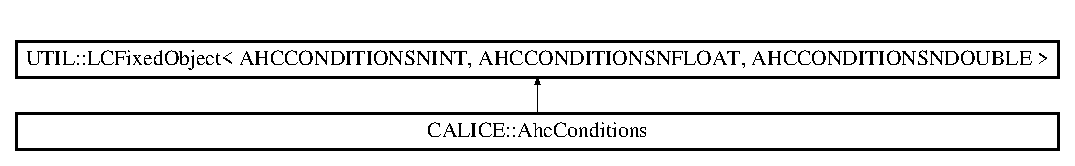
\includegraphics[height=1.789137cm]{classCALICE_1_1AhcConditions}
\end{center}
\end{figure}
\subsection*{Public Member Functions}
\begin{DoxyCompactItemize}
\item 
{\bf Ahc\-Conditions} ()\label{classCALICE_1_1AhcConditions_af6aea1e5d883dead6639e3be18b13f76}

\begin{DoxyCompactList}\small\item\em default constructor \end{DoxyCompactList}\item 
{\bf Ahc\-Conditions} (int module\-Nr, unsigned module\-I\-D, int calib\-Start, int calib\-Width, bool calib\-Enable, int hold, int hold\-Width, int multiplex, int vcalib, int verification, int sr[12])
\begin{DoxyCompactList}\small\item\em constructor, \doxyref{Ahc\-Conditions}{p.}{classCALICE_1_1AhcConditions} is initialized with the parameters given \end{DoxyCompactList}\item 
{\bfseries Ahc\-Conditions} (L\-C\-Object $\ast$obj)\label{classCALICE_1_1AhcConditions_ae1b844aa093496edbafaebc8f7c3e53e}

\item 
unsigned {\bf get\-Module\-I\-D} () const \label{classCALICE_1_1AhcConditions_afd54d91c0e7e95542cd9a625381c4c5a}

\begin{DoxyCompactList}\small\item\em get module I\-D of config \end{DoxyCompactList}\item 
unsigned {\bf get\-Module\-Nr} ()\label{classCALICE_1_1AhcConditions_ae8e8f7b251aa4c2d05259543b68eb774}

\begin{DoxyCompactList}\small\item\em get module number of config \end{DoxyCompactList}\item 
unsigned {\bf get\-Calib\-Start} () const \label{classCALICE_1_1AhcConditions_a2ac195704d21b51193059a17a5c2f1b4}

\begin{DoxyCompactList}\small\item\em get calib start \end{DoxyCompactList}\item 
unsigned {\bf get\-Calib\-Width} () const \label{classCALICE_1_1AhcConditions_ab2bf4d8631141459c3d7091e88a7e72c}

\begin{DoxyCompactList}\small\item\em get calib width \end{DoxyCompactList}\item 
bool {\bf is\-Calib\-Enabled} () const \label{classCALICE_1_1AhcConditions_a8456b8157c53f61749215c47f536e24e}

\begin{DoxyCompactList}\small\item\em get if calib is enabled \end{DoxyCompactList}\item 
float {\bf get\-Hold} () const \label{classCALICE_1_1AhcConditions_a725c4a0227fdb1a73859fcae2666f761}

\begin{DoxyCompactList}\small\item\em get hold \end{DoxyCompactList}\item 
unsigned {\bf get\-Hold\-Width} () const \label{classCALICE_1_1AhcConditions_a1e08962a2ddb922dbcfaf88fac024662}

\begin{DoxyCompactList}\small\item\em get hold width \end{DoxyCompactList}\item 
unsigned {\bf get\-Multiplex} () const \label{classCALICE_1_1AhcConditions_abc2849f2554962e03e62d633afaa4553}

\begin{DoxyCompactList}\small\item\em get order of multiplexing \end{DoxyCompactList}\item 
unsigned {\bf get\-Vcalib} () const \label{classCALICE_1_1AhcConditions_a7a3ebe5695fb349e015ddc12a4ab800f}

\begin{DoxyCompactList}\small\item\em get vcalib \end{DoxyCompactList}\item 
unsigned {\bf get\-Verification} () const \label{classCALICE_1_1AhcConditions_a792d5b3e5a9b31e40ffe9ea0c38a062a}

\begin{DoxyCompactList}\small\item\em get verification data \end{DoxyCompactList}\item 
unsigned {\bf get\-S\-R} (unsigned hab) const \label{classCALICE_1_1AhcConditions_a1521056060193303fb7c85657a005c1e}

\begin{DoxyCompactList}\small\item\em get hab sr \end{DoxyCompactList}\item 
void {\bf print} (std\-::ostream \&os)\label{classCALICE_1_1AhcConditions_a742f77cfa0886de4f4ff2ee0bde9900d}

\begin{DoxyCompactList}\small\item\em convenient print method \end{DoxyCompactList}\item 
const std\-::string {\bf get\-Type\-Name} () const \label{classCALICE_1_1AhcConditions_a6c7d11954356e9c4ac64a46525bb54ff}

\begin{DoxyCompactList}\small\item\em return the type of the class \end{DoxyCompactList}\item 
const std\-::string {\bf get\-Data\-Description} () const \label{classCALICE_1_1AhcConditions_a31282cd05d783c18c6593f731e9fa24d}

\begin{DoxyCompactList}\small\item\em return a brief description of the data memeber \end{DoxyCompactList}\end{DoxyCompactItemize}


\subsection{Detailed Description}
Class for the \doxyref{C\-A\-L\-I\-C\-E}{p.}{namespaceCALICE} Ahcal conditions information during the reconstruction. 

renamed from \doxyref{Calice\-Conditions}{p.}{classCALICE_1_1CaliceConditions} 2007/12/14 B.\-Lutz

Information is stored module wise \begin{DoxyAuthor}{Author}
B. Lutz D\-E\-S\-Y 
\end{DoxyAuthor}
\begin{DoxyDate}{Date}
Sep 11 2006 
\end{DoxyDate}


Definition at line 32 of file Ahc\-Conditions.\-hh.



\subsection{Constructor \& Destructor Documentation}
\index{C\-A\-L\-I\-C\-E\-::\-Ahc\-Conditions@{C\-A\-L\-I\-C\-E\-::\-Ahc\-Conditions}!Ahc\-Conditions@{Ahc\-Conditions}}
\index{Ahc\-Conditions@{Ahc\-Conditions}!CALICE::AhcConditions@{C\-A\-L\-I\-C\-E\-::\-Ahc\-Conditions}}
\subsubsection[{Ahc\-Conditions}]{\setlength{\rightskip}{0pt plus 5cm}C\-A\-L\-I\-C\-E\-::\-Ahc\-Conditions\-::\-Ahc\-Conditions (
\begin{DoxyParamCaption}
\item[{int}]{module\-Nr, }
\item[{unsigned}]{module\-I\-D, }
\item[{int}]{calib\-Start, }
\item[{int}]{calib\-Width, }
\item[{bool}]{calib\-Enable, }
\item[{int}]{hold, }
\item[{int}]{hold\-Width, }
\item[{int}]{multiplex, }
\item[{int}]{vcalib, }
\item[{int}]{verification, }
\item[{int}]{sr[12]}
\end{DoxyParamCaption}
)\hspace{0.3cm}{\ttfamily [inline]}}\label{classCALICE_1_1AhcConditions_a51eb529321a6006fb0b9d46046ba056a}


constructor, \doxyref{Ahc\-Conditions}{p.}{classCALICE_1_1AhcConditions} is initialized with the parameters given 


\begin{DoxyParams}{Parameters}
{\em module\-Nr} & mdoule \char`\"{}stamp\char`\"{} \\
\hline
{\em module\-I\-D} & module I\-D of the module the hit is in, low byte gives upper or lower half, high byte gives module \char`\"{}stamp\char`\"{}, used to find correct calibration \\
\hline
{\em calib\-Start} & starting time of Tcalib signal in ticks \\
\hline
{\em calib\-Width} & duration of the Tcalib signal in ticks \\
\hline
{\em calib\-Enable} & has Tcalib signal been sent at all? \\
\hline
{\em hold} & starting time of the hold signal in ticks (6.\-25ns) \\
\hline
{\em hold\-Width} & duration of the hold signal in ticks (6.\-25ns) \\
\hline
{\em multiplex} & number of multiplexed signals in the acquisition cycle \\
\hline
{\em vcalib} & Vcalib value \\
\hline
{\em verification} & shift register verification pattern \\
\hline
{\em sr} & shift registers \\
\hline
\end{DoxyParams}


Definition at line 54 of file Ahc\-Conditions.\-hh.



The documentation for this class was generated from the following files\-:\begin{DoxyCompactItemize}
\item 
Ahc\-Conditions.\-hh\item 
Ahc\-Conditions.\-cc\end{DoxyCompactItemize}

\section{C\-A\-L\-I\-C\-E\-:\-:Ahc\-Mapper Class Reference}
\label{classCALICE_1_1AhcMapper}\index{C\-A\-L\-I\-C\-E\-::\-Ahc\-Mapper@{C\-A\-L\-I\-C\-E\-::\-Ahc\-Mapper}}


A\-H\-C\-A\-L implementation of \doxyref{Mapper}{p.}{classCALICE_1_1Mapper} class.  




{\ttfamily \#include $<$Ahc\-Mapper.\-hh$>$}

Inheritance diagram for C\-A\-L\-I\-C\-E\-:\-:Ahc\-Mapper\-:\begin{figure}[H]
\begin{center}
\leavevmode
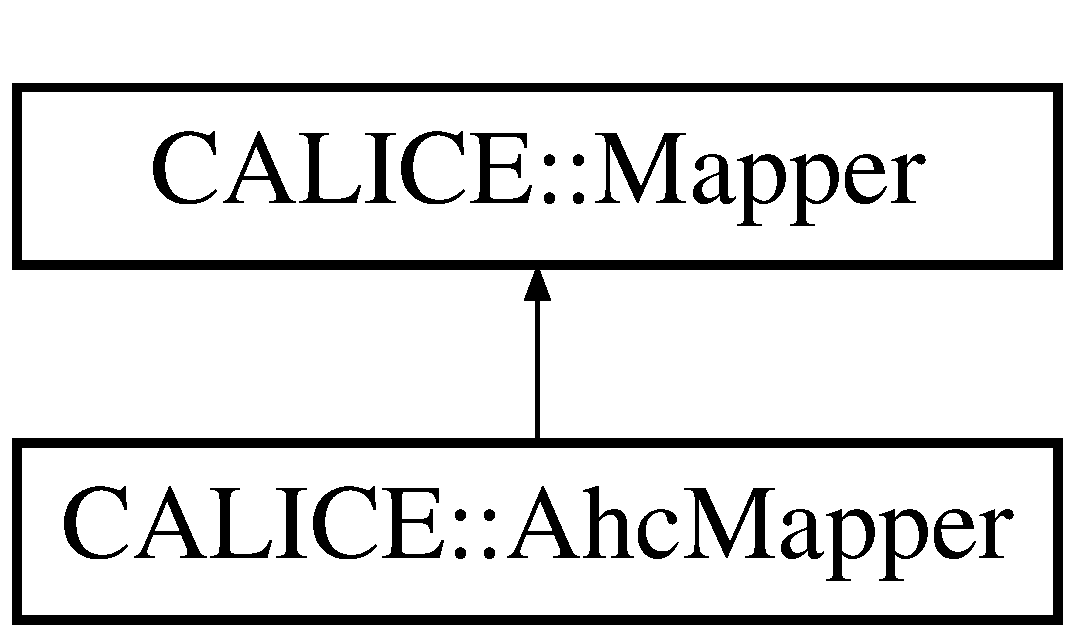
\includegraphics[height=2.000000cm]{classCALICE_1_1AhcMapper}
\end{center}
\end{figure}
\subsection*{Public Member Functions}
\begin{DoxyCompactItemize}
\item 
int {\bf get\-Cell\-I\-D\-From\-Mod\-Chip\-Chan} (const unsigned int module, const unsigned int chip, const unsigned int channel) const 
\begin{DoxyCompactList}\small\item\em generate (Mokka) cell\-I\-D from module, chip, channel \end{DoxyCompactList}\item 
unsigned int {\bf get\-Module\-From\-Cell\-I\-D} (const int cell\-I\-D) const 
\begin{DoxyCompactList}\small\item\em module number from (Mokka) Cell\-I\-D \end{DoxyCompactList}\item 
unsigned int {\bf get\-Module\-From\-D\-A\-Q\-I\-D} (const int D\-A\-Qchannel) const 
\begin{DoxyCompactList}\small\item\em module number from D\-A\-Q channel I\-D \end{DoxyCompactList}\item 
unsigned int {\bf get\-Module} (const unsigned int crate, const unsigned int slot, const unsigned int fe) const 
\begin{DoxyCompactList}\small\item\em module number from triple crate, slot, fe \end{DoxyCompactList}\item 
unsigned int {\bf get\-Module} (const unsigned int k) const 
\begin{DoxyCompactList}\small\item\em module number from K \end{DoxyCompactList}\item 
unsigned int {\bf get\-Module\-From\-Cell\-I\-D} (const int cell\-I\-D, bool \&valid) const 
\begin{DoxyCompactList}\small\item\em get module (number) in which this cell is included from (Mokka) cell\-I\-D \end{DoxyCompactList}\item 
unsigned int {\bf get\-Module\-From\-D\-A\-Q\-I\-D} (const int D\-A\-Qchannel, bool \&valid) const 
\begin{DoxyCompactList}\small\item\em get module (number) in which this (D\-A\-Q) channel is included \end{DoxyCompactList}\item 
unsigned int {\bf get\-Module\-From\-Module\-I\-D} (const int module\-I\-D, bool \&valid) const 
\begin{DoxyCompactList}\small\item\em get module (number) from this (module) channel I\-D \end{DoxyCompactList}\item 
unsigned int {\bf get\-Chip\-From\-Cell\-I\-D} (const int cell\-I\-D) const 
\begin{DoxyCompactList}\small\item\em chip number from (Mokka) Cell\-I\-D \end{DoxyCompactList}\item 
unsigned int {\bf get\-Chip} (const unsigned int i, const unsigned int j, const unsigned int k) const 
\begin{DoxyCompactList}\small\item\em chip number from triple I, J, K \end{DoxyCompactList}\item 
unsigned int {\bf get\-Chan\-From\-Cell\-I\-D} (const int cell\-I\-D) const 
\begin{DoxyCompactList}\small\item\em channel number from (Mokka) Cell\-I\-D \end{DoxyCompactList}\item 
unsigned int {\bf get\-Chan} (const unsigned int i, const unsigned int j, const unsigned int k) const 
\begin{DoxyCompactList}\small\item\em chip number from triple I, J, K \end{DoxyCompactList}\item 
unsigned int {\bf get\-Crate\-From\-Cell\-I\-D} (const int cell\-I\-D) const 
\begin{DoxyCompactList}\small\item\em crate number from (Mokka) Cell\-I\-D \end{DoxyCompactList}\item 
unsigned int {\bf get\-Crate\-From\-Module\-I\-D} (const int module\-I\-D) const 
\begin{DoxyCompactList}\small\item\em crate number from Module cell I\-D \end{DoxyCompactList}\item 
unsigned int {\bf get\-Crate} (const unsigned int module) const 
\begin{DoxyCompactList}\small\item\em crate number from module number \end{DoxyCompactList}\item 
unsigned int {\bf get\-Slot\-From\-Cell\-I\-D} (const int cell\-I\-D) const 
\begin{DoxyCompactList}\small\item\em slot number from (Mokka) Cell\-I\-D \end{DoxyCompactList}\item 
unsigned int {\bf get\-Slot\-From\-Module\-I\-D} (const int module\-I\-D) const 
\begin{DoxyCompactList}\small\item\em slot number from Module cell I\-D \end{DoxyCompactList}\item 
unsigned int {\bf get\-Slot} (const unsigned int module) const 
\begin{DoxyCompactList}\small\item\em slot number from module number \end{DoxyCompactList}\item 
unsigned int {\bf get\-Fe\-From\-Cell\-I\-D} (const int cell\-I\-D) const 
\begin{DoxyCompactList}\small\item\em front end number from (Mokka) Cell\-I\-D \end{DoxyCompactList}\item 
unsigned int {\bf get\-Fe\-From\-Module\-I\-D} (const int module\-I\-D) const 
\begin{DoxyCompactList}\small\item\em front end number from Module cell I\-D \end{DoxyCompactList}\item 
unsigned int {\bf get\-Fe} (const unsigned int module) const 
\begin{DoxyCompactList}\small\item\em front end number from module number \end{DoxyCompactList}\item 
unsigned int {\bf get\-I\-From\-Module\-I\-D} (const int module\-I\-D) const 
\begin{DoxyCompactList}\small\item\em I of (Mokka) cell\-I\-D. \end{DoxyCompactList}\item 
unsigned int {\bf get\-I\-From\-D\-A\-Q\-I\-D} (const int D\-A\-Qchannel) const 
\begin{DoxyCompactList}\small\item\em I of (Mokka) cell\-I\-D. \end{DoxyCompactList}\item 
unsigned int {\bf get\-I} (const unsigned int module, const unsigned int chip, const unsigned int chan) const 
\begin{DoxyCompactList}\small\item\em I of (Mokka) cell\-I\-D. \end{DoxyCompactList}\item 
unsigned int {\bf get\-J\-From\-Module\-I\-D} (const int module\-I\-D) const 
\begin{DoxyCompactList}\small\item\em J of (Mokka) cell\-I\-D. \end{DoxyCompactList}\item 
unsigned int {\bf get\-J\-From\-D\-A\-Q\-I\-D} (const int D\-A\-Qchannel) const 
\begin{DoxyCompactList}\small\item\em J of (Mokka) cell\-I\-D. \end{DoxyCompactList}\item 
unsigned int {\bf get\-J} (const unsigned int module, const unsigned chip, const unsigned chan) const 
\begin{DoxyCompactList}\small\item\em J of (Mokka) cell\-I\-D. \end{DoxyCompactList}\item 
unsigned int {\bf get\-K\-From\-Module\-I\-D} (const int module\-I\-D) const 
\begin{DoxyCompactList}\small\item\em K of (Mokka) cell\-I\-D. \end{DoxyCompactList}\item 
unsigned int {\bf get\-K\-From\-D\-A\-Q\-I\-D} (const int D\-A\-Qchannel) const 
\begin{DoxyCompactList}\small\item\em K of (Mokka) cell\-I\-D. \end{DoxyCompactList}\item 
unsigned int {\bf get\-K} (const unsigned int module) const 
\begin{DoxyCompactList}\small\item\em K of (Mokka) cell\-I\-D. \end{DoxyCompactList}\item 
unsigned int {\bf get\-I\-Size\-From\-Cell\-I\-D} (const int cell\-I\-D) const 
\begin{DoxyCompactList}\small\item\em get cell size in I direction of (Mokka) Cell\-I\-D coordinate \end{DoxyCompactList}\item 
unsigned int {\bf get\-I\-Size\-From\-Module\-I\-D} (const int module\-I\-D) const 
\begin{DoxyCompactList}\small\item\em get cell size in I direction of (Mokka) Cell\-I\-D coordinate \end{DoxyCompactList}\item 
unsigned int {\bf get\-I\-Size\-From\-D\-A\-Q\-I\-D} (const int D\-A\-Qchannel) const 
\begin{DoxyCompactList}\small\item\em get cell size in I direction of (Mokka) Cell\-I\-D coordinate \end{DoxyCompactList}\item 
unsigned int {\bf get\-I\-Size\-From\-I\-J\-K} (const unsigned int i, const unsigned int j, const unsigned int k) const 
\begin{DoxyCompactList}\small\item\em get cell size in I direction of (Mokka) Cell\-I\-D coordinate \end{DoxyCompactList}\item 
unsigned int {\bf get\-I\-Size} (const unsigned int module, const unsigned int chip, const unsigned int chan) const 
\begin{DoxyCompactList}\small\item\em get cell size in I direction of (Mokka) Cell\-I\-D coordinate \end{DoxyCompactList}\item 
unsigned int {\bf get\-J\-Size\-From\-Cell\-I\-D} (const int cell\-I\-D) const 
\begin{DoxyCompactList}\small\item\em get cell size in J direction of (Mokka) Cell\-I\-D coordinate \end{DoxyCompactList}\item 
unsigned int {\bf get\-J\-Size\-From\-Module\-I\-D} (const int module\-I\-D) const 
\begin{DoxyCompactList}\small\item\em get cell size in J direction of (Mokka) Cell\-I\-D coordinate \end{DoxyCompactList}\item 
unsigned int {\bf get\-J\-Size\-From\-D\-A\-Q\-I\-D} (const int D\-A\-Qchannel) const 
\begin{DoxyCompactList}\small\item\em get cell size in J direction of (Mokka) Cell\-I\-D coordinate \end{DoxyCompactList}\item 
unsigned int {\bf get\-J\-Size\-From\-I\-J\-K} (const unsigned int i, const unsigned int j, const unsigned int k) const 
\begin{DoxyCompactList}\small\item\em get cell size in J direction of (Mokka) Cell\-I\-D coordinate \end{DoxyCompactList}\item 
unsigned int {\bf get\-J\-Size} (const unsigned int module, const unsigned int chip, const unsigned int chan) const 
\begin{DoxyCompactList}\small\item\em get cell size in J direction of (Mokka) Cell\-I\-D coordinate \end{DoxyCompactList}\item 
int {\bf get\-True\-Cell\-I\-D} (const int virtual\-Cell\-Index) const 
\begin{DoxyCompactList}\small\item\em return identifying index of cell \end{DoxyCompactList}\item 
int {\bf get\-True\-Cell\-I\-D} (const unsigned int i, const unsigned int j, const unsigned int k) const 
\begin{DoxyCompactList}\small\item\em return identifying index of cell \end{DoxyCompactList}\item 
unsigned int {\bf get\-True\-I\-From\-Cell\-I\-D} (const int virtual\-Cell\-I\-D) const 
\begin{DoxyCompactList}\small\item\em return I of identifying index of cell \end{DoxyCompactList}\item 
unsigned int {\bf get\-True\-I\-From\-I\-J\-K} (const unsigned int i, const unsigned int j, const unsigned int k) const 
\begin{DoxyCompactList}\small\item\em return I of identifying index of cell \end{DoxyCompactList}\item 
unsigned int {\bf get\-True\-I} (const unsigned int module, const unsigned int i, const unsigned int j) const 
\begin{DoxyCompactList}\small\item\em return I of identifying index of cell \end{DoxyCompactList}\item 
unsigned int {\bf get\-True\-J\-From\-Cell\-I\-D} (const int virtual\-Cell\-I\-D) const 
\begin{DoxyCompactList}\small\item\em return J of identifying index of cell \end{DoxyCompactList}\item 
unsigned int {\bf get\-True\-J\-From\-I\-J\-K} (const unsigned int i, const unsigned int j, const unsigned int k) const 
\begin{DoxyCompactList}\small\item\em return J of identifying index of cell \end{DoxyCompactList}\item 
unsigned int {\bf get\-True\-J} (const unsigned int module, const unsigned int i, const unsigned int j) const 
\begin{DoxyCompactList}\small\item\em return J of identifying index of cell \end{DoxyCompactList}\item 
unsigned int {\bf get\-Max\-Module} () const 
\begin{DoxyCompactList}\small\item\em return maximum module number \end{DoxyCompactList}\item 
unsigned int {\bf get\-Max\-Chip} () const 
\begin{DoxyCompactList}\small\item\em return maximum chip number \end{DoxyCompactList}\item 
unsigned int {\bf get\-Max\-Channel} () const 
\begin{DoxyCompactList}\small\item\em return maximum channel number \end{DoxyCompactList}\item 
unsigned int {\bf get\-Max\-I} () const 
\begin{DoxyCompactList}\small\item\em return maximum I index \end{DoxyCompactList}\item 
unsigned int {\bf get\-Max\-J} () const 
\begin{DoxyCompactList}\small\item\em return maximum J index \end{DoxyCompactList}\item 
unsigned int {\bf get\-Max\-K} () const 
\begin{DoxyCompactList}\small\item\em return maximum K index \end{DoxyCompactList}\item 
void {\bf fill} (const lcio\-::\-L\-C\-Collection $\ast$module\-Description\-Col, const lcio\-::\-L\-C\-Collection $\ast$module\-Connection\-Col)
\begin{DoxyCompactList}\small\item\em fills all necessary mapping information \end{DoxyCompactList}\item 
void {\bf update\-Connections} (const lcio\-::\-L\-C\-Collection $\ast$module\-Connection\-Col)
\begin{DoxyCompactList}\small\item\em updates the mapping information in the class (possible after first fill only) \end{DoxyCompactList}\item 
void {\bf print} (std\-::ostream \&ostream) const 
\begin{DoxyCompactList}\small\item\em print current data contents \end{DoxyCompactList}\item 
void {\bf print\-Stats} (std\-::ostream \&ostream) const 
\begin{DoxyCompactList}\small\item\em print summary of current data contents \end{DoxyCompactList}\end{DoxyCompactItemize}
\subsection*{Protected Member Functions}
\begin{DoxyCompactItemize}
\item 
unsigned int {\bf get\-Index\-By\-Cell\-I\-D} (const int cell\-I\-D) const 
\begin{DoxyCompactList}\small\item\em get a compact index for storing data in vectors \end{DoxyCompactList}\item 
unsigned int {\bf get\-Index\-By\-D\-A\-Q\-I\-D} (const int I\-D) const 
\begin{DoxyCompactList}\small\item\em get a compact index for storing data in vectors \end{DoxyCompactList}\item 
unsigned int {\bf get\-Index\-By\-Module\-I\-D} (const int I\-D) const 
\begin{DoxyCompactList}\small\item\em get a compact index for storing data in vectors \end{DoxyCompactList}\item 
unsigned int {\bf get\-Max\-Index} () const 
\begin{DoxyCompactList}\small\item\em get the maximum value of the compact index for storing data in vectors \end{DoxyCompactList}\item 
int {\bf get\-Cell\-I\-D\-Of\-Index} (unsigned int index) const 
\begin{DoxyCompactList}\small\item\em get the cell I\-D of a certain compact index \end{DoxyCompactList}\end{DoxyCompactItemize}
\subsection*{Private Types}
\begin{DoxyCompactItemize}
\item 
typedef std\-::map$<$ unsigned int, \\*
unsigned int $>$ {\bfseries index\-Map\-\_\-t}\label{classCALICE_1_1AhcMapper_aeeed74906b2af733e9892f881e1e10f4}

\end{DoxyCompactItemize}
\subsection*{Private Member Functions}
\begin{DoxyCompactItemize}
\item 
bool {\bfseries valid} (const unsigned int index, const std\-::vector$<$ bool $>$ \&available\-Vec) const \label{classCALICE_1_1AhcMapper_a74df7b7905102cd68455c8fbb1b69d7e}

\item 
bool {\bfseries valid} (const unsigned int index, const index\-Map\-\_\-t \&index\-Map) const \label{classCALICE_1_1AhcMapper_aa9eeded28b325b54d4a532fc645e5af4}

\item 
unsigned int {\bfseries get\-Module\-Type\-Index} (const unsigned int module) const \label{classCALICE_1_1AhcMapper_aab9e59fb5ea9b3796a01ad47d52bc1f6}

\item 
unsigned int {\bfseries get\-Index\-Module\-Connection} (const unsigned int crate, const unsigned int slot, const unsigned int fe) const \label{classCALICE_1_1AhcMapper_a8971d066c71198c8bf247bfee592349a}

\item 
unsigned int {\bfseries get\-Crate\-From\-Module\-Connection\-Index} (const unsigned int index) const \label{classCALICE_1_1AhcMapper_a3222ce7720aef1e7731426231e433452}

\item 
unsigned int {\bfseries get\-Slot\-From\-Module\-Connection\-Index} (const unsigned int index) const \label{classCALICE_1_1AhcMapper_a9b25bfccd367acde37bae9b90e1d622e}

\item 
unsigned int {\bfseries get\-Fe\-From\-Module\-Connection\-Index} (const unsigned int index) const \label{classCALICE_1_1AhcMapper_ad7258974e1fe5e8127b32b42619e2d1f}

\item 
unsigned int {\bfseries get\-Compact\-Index} (const unsigned int module, const unsigned int chip, const unsigned int chan) const \label{classCALICE_1_1AhcMapper_aab353949bad76aaf654e41da8deae82c}

\item 
unsigned int {\bfseries get\-Compact\-Index} (const unsigned int module, const unsigned int chan\-Index) const \label{classCALICE_1_1AhcMapper_ae37272cef13cfad682728dafb3d2324a}

\item 
unsigned int {\bfseries get\-Module\-From\-Compact\-Index} (const unsigned int index) const \label{classCALICE_1_1AhcMapper_ae9f81a2a43b50256d8950a11a88fa275}

\item 
unsigned int {\bfseries get\-Chip\-From\-Compact\-Index} (const unsigned int index) const \label{classCALICE_1_1AhcMapper_ad18f22334b7691c9b60855d2d63008a3}

\item 
unsigned int {\bfseries get\-Chan\-From\-Compact\-Index} (const unsigned int index) const \label{classCALICE_1_1AhcMapper_ae7a2539be4244d7fd0cdcf4afac85ad0}

\item 
unsigned int {\bfseries get\-Module\-From\-Index} (const unsigned int index, bool \&valid) const \label{classCALICE_1_1AhcMapper_a56c48aba41a7c726a457c7653eeb1a5c}

\item 
unsigned int {\bfseries get\-Index\-Chan} (const unsigned int chip, const unsigned int chan) const \label{classCALICE_1_1AhcMapper_a4a8f47ef57d76bd9fb2c23f27a7c6451}

\item 
unsigned int {\bfseries get\-Chip\-From\-Chan\-Index} (const unsigned int index) const \label{classCALICE_1_1AhcMapper_a2324012066d0903ba23d5f96d35b1c78}

\item 
unsigned int {\bfseries get\-Chan\-From\-Chan\-Index} (const unsigned int index) const \label{classCALICE_1_1AhcMapper_ac06830ea38f15374a584208d4a40f86a}

\item 
unsigned int {\bfseries get\-Index\-I\-J} (const unsigned int i, const unsigned int j) const \label{classCALICE_1_1AhcMapper_a204172bf4005d14c1bd7b70df98186d3}

\item 
unsigned int {\bfseries get\-I\-From\-I\-J\-Index} (const unsigned int index) const \label{classCALICE_1_1AhcMapper_a32cb7e27e0ae8867fb64b3217e8b4dac}

\item 
unsigned int {\bfseries get\-J\-From\-I\-J\-Index} (const unsigned int index) const \label{classCALICE_1_1AhcMapper_adcd54575e64211dc80da66e269834daa}

\item 
void {\bfseries clear\-Crate} ()\label{classCALICE_1_1AhcMapper_aefa941cea97ef01e1f400fd82cbd36f8}

\item 
void {\bfseries clear\-Slot} ()\label{classCALICE_1_1AhcMapper_a79794d916def06030787c9f288aa2bad}

\item 
void {\bfseries clear\-Module\-Type} ()\label{classCALICE_1_1AhcMapper_a024182c2a5e1ad79e0a9de21fc8a11d7}

\item 
{\footnotesize template$<$class T $>$ }\\void {\bfseries init\-To\-Size} (std\-::vector$<$ T $>$ \&vec, const unsigned int size, const T init\-Value)\label{classCALICE_1_1AhcMapper_a83f60c207caeac8ec658e5f569f478dd}

\item 
void {\bfseries init\-To\-Size} (std\-::vector$<$ bool $>$ \&vec, const unsigned int size)\label{classCALICE_1_1AhcMapper_a383c4627b641162bb5d7b78c60c3989a}

\item 
void {\bfseries init\-To\-Size} (std\-::vector$<$ unsigned int $>$ \&data\-Vec, std\-::vector$<$ bool $>$ \&available\-Vec, const unsigned int size)\label{classCALICE_1_1AhcMapper_ad6b97628b5c5e4db1fc12cee65cc3f4d}

\item 
void {\bfseries init\-Fe} (const unsigned int max\-Fe=0)\label{classCALICE_1_1AhcMapper_ad15c4051d56f20ffc66e0b5d52f81890}

\item 
void {\bfseries init\-Module} (const unsigned int max\-Mod=0)\label{classCALICE_1_1AhcMapper_af15a8d86b8f3d9210b0899a0ee1f218e}

\item 
void {\bfseries init\-K} (const unsigned int max\-K=0)\label{classCALICE_1_1AhcMapper_a76e45ca5b0e1e2706c49f6c8250a0d38}

\item 
void {\bfseries init\-I\-J\-Chip\-Channel} (const unsigned int max\-I=0, const unsigned int max\-J=0, const unsigned int max\-Chip=0, const unsigned int max\-Chan=0)\label{classCALICE_1_1AhcMapper_a65d452691dedf5bb9fecddf3bfb444b4}

\item 
void {\bfseries clear} ()\label{classCALICE_1_1AhcMapper_ac1442af64ad70eb7d0a1b7fc4c7f53b6}

\item 
void {\bfseries register\-Crate} (const unsigned int crate)\label{classCALICE_1_1AhcMapper_ac58c61c50764da525db379b0d1fc9294}

\item 
bool {\bfseries crate\-Available} (const unsigned int crate) const \label{classCALICE_1_1AhcMapper_ae477476123f13062074f2b9c650bb9b1}

\item 
void {\bfseries register\-Slot} (const unsigned int slot)\label{classCALICE_1_1AhcMapper_a41134f8aced6392e03c901a73ea9ee2a}

\item 
bool {\bfseries slot\-Available} (const unsigned int slot) const \label{classCALICE_1_1AhcMapper_a881f7bb684650d934f3e3f4712b89ee7}

\item 
void {\bfseries register\-Module\-Type} (const unsigned int module\-Type\-Name)\label{classCALICE_1_1AhcMapper_a45518c038310ae5493d7012d40664725}

\item 
bool {\bfseries module\-Type\-Available} (const unsigned int module\-Type\-Name) const \label{classCALICE_1_1AhcMapper_a81729b3b42e81d44cd31b29c95707f9e}

\item 
unsigned int {\bfseries count\-Available} (const std\-::vector$<$ bool $>$ \&vec) const \label{classCALICE_1_1AhcMapper_aac91ec43c8273688216ae604ac05e895}

\item 
void {\bfseries set\-Module\-Crate\-Slot\-Fe} (const unsigned int module, const unsigned int crate, const unsigned int slot, const unsigned int fe)\label{classCALICE_1_1AhcMapper_a4d3085baa30407cb160fc33c9c78bcd2}

\item 
void {\bfseries set\-Module\-Type} (const unsigned int module, const unsigned int type\-Name)\label{classCALICE_1_1AhcMapper_a2b871dd10848faae136940c12ca27bd9}

\item 
void {\bfseries set\-Module\-K} (const unsigned int module, const unsigned int K)\label{classCALICE_1_1AhcMapper_a08953a9ae064d95675d9cd0a749570a6}

\item 
void {\bfseries set\-Module\-Type\-I\-J\-Chip\-Channel} (const unsigned int module\-Type\-Name, const unsigned int I, const unsigned int J, const unsigned int size\-I, const unsigned int size\-J, const unsigned int chip, const unsigned int channel)\label{classCALICE_1_1AhcMapper_a73d414346acc2e03052b22fabc050d86}

\item 
void {\bf fill\-Module\-Connection} (const lcio\-::\-L\-C\-Collection $\ast$col)
\begin{DoxyCompactList}\small\item\em sets the mapping information in the class, call after fill\-Module\-Description \end{DoxyCompactList}\item 
void {\bf fill\-Module\-Description} (const lcio\-::\-L\-C\-Collection $\ast$col)
\begin{DoxyCompactList}\small\item\em sets the module layout information in the class, module connection information will be invalidated \end{DoxyCompactList}\item 
void {\bfseries get\-Chip\-Channel\-For\-Module\-Description\-I\-D} (const unsigned int id, const unsigned int module\-Type, int \&chip, int \&channel) const \label{classCALICE_1_1AhcMapper_a8a11bbe860cd7085fbc975bfcc791c37}

\item 
unsigned int {\bfseries get\-Combined\-Module\-Type} (const unsigned int module\-Type) const \label{classCALICE_1_1AhcMapper_a8749cdfa53ef252ff887bfec78d5830b}

\item 
int {\bfseries correct\-Cell\-Index} (const unsigned int module\-Type, const int cell\-Index) const \label{classCALICE_1_1AhcMapper_a6469d9f7071f5ebb451530e41b5660a5}

\item 
const std\-::string {\bfseries print\-If\-Available} (bool available, unsigned int value) const \label{classCALICE_1_1AhcMapper_ad775b776bc11616feafa9402b4d0f489}

\end{DoxyCompactItemize}
\subsection*{Private Attributes}
\begin{DoxyCompactItemize}
\item 
unsigned int {\bfseries \-\_\-n\-Chan}\label{classCALICE_1_1AhcMapper_ad1223d57d472b9a1a47d0cdc58b2e4d7}

\item 
unsigned int {\bfseries \-\_\-n\-Chip}\label{classCALICE_1_1AhcMapper_acca5e6401c3930c7bd0a629ee3f93178}

\item 
unsigned int {\bfseries \-\_\-n\-Fe}\label{classCALICE_1_1AhcMapper_a0d39db3b164e7810a9ce1bec289a1410}

\item 
unsigned int {\bfseries \-\_\-n\-Slot}\label{classCALICE_1_1AhcMapper_a298cc6f721fe2a76514a49e83831f4e3}

\item 
unsigned int {\bfseries \-\_\-max\-Slot}\label{classCALICE_1_1AhcMapper_a51ef6086881b08eb51ca5af2bdcfcf83}

\item 
unsigned int {\bfseries \-\_\-n\-Crate}\label{classCALICE_1_1AhcMapper_a012ef86ff01b044e8c33b9871ecbc4b3}

\item 
unsigned int {\bfseries \-\_\-n\-Mod}\label{classCALICE_1_1AhcMapper_a1f91d835a24d504011715fc7cecd4a8e}

\item 
unsigned int {\bfseries \-\_\-n\-Mod\-Type}\label{classCALICE_1_1AhcMapper_a30c33cb167b3062406eaa4a51ef5b64f}

\item 
unsigned int {\bfseries \-\_\-n\-I}\label{classCALICE_1_1AhcMapper_a1df3b36a1945b9e16283de7159f61a4e}

\item 
unsigned int {\bfseries \-\_\-n\-J}\label{classCALICE_1_1AhcMapper_a2228494a778640c420afe67f81f4c030}

\item 
unsigned int {\bfseries \-\_\-n\-K}\label{classCALICE_1_1AhcMapper_aa20c4b918afca46a0315529efb2263a0}

\item 
index\-Map\-\_\-t {\bfseries \-\_\-crate\-Index}\label{classCALICE_1_1AhcMapper_a141fb6ec8b5c668ed3ad02edb89c8e0c}

\item 
std\-::vector$<$ unsigned int $>$ {\bfseries \-\_\-crate\-Number}\label{classCALICE_1_1AhcMapper_a9bcc209bc9a2cd2208451d9e7e98168f}

\item 
std\-::vector$<$ unsigned int $>$ {\bfseries \-\_\-slot\-Index}\label{classCALICE_1_1AhcMapper_a870803394fbfaf449dc5e3a9564abebf}

\item 
std\-::vector$<$ unsigned int $>$ {\bfseries \-\_\-slot\-Number}\label{classCALICE_1_1AhcMapper_ad2acb33e40a070102170ba90c90ac5df}

\item 
std\-::vector$<$ bool $>$ {\bfseries \-\_\-slot\-Available}\label{classCALICE_1_1AhcMapper_ad45184245e1c6716113883282fee77ad}

\item 
std\-::vector$<$ bool $>$ {\bfseries \-\_\-connection\-Available}\label{classCALICE_1_1AhcMapper_a0ef975b1772d9da449e18a94535a6ebc}

\item 
std\-::vector$<$ bool $>$ {\bfseries \-\_\-module\-Available}\label{classCALICE_1_1AhcMapper_a45ba28e98649b1f4956548e266537db3}

\item 
std\-::vector$<$ unsigned int $>$ {\bfseries \-\_\-type\-Vmodule}\label{classCALICE_1_1AhcMapper_a165279f2c79fc7bdaa6c5b33186d7174}

\item 
std\-::vector$<$ unsigned int $>$ {\bfseries \-\_\-connection\-Vmodule}\label{classCALICE_1_1AhcMapper_a210096c9fb1c3286b2a07e7fcfc3d1f8}

\item 
std\-::vector$<$ bool $>$ {\bfseries \-\_\-connection\-Vmodule\-Available}\label{classCALICE_1_1AhcMapper_ad03313bc91520da24585f0e3c5f33342}

\item 
std\-::vector$<$ unsigned int $>$ {\bfseries \-\_\-module\-Vconnection}\label{classCALICE_1_1AhcMapper_a9492ae109cabc3256c81d0ead4282422}

\item 
std\-::vector$<$ unsigned int $>$ {\bfseries \-\_\-k\-Vmodule}\label{classCALICE_1_1AhcMapper_a6c6557dbf072ae4742a2ead776a24d33}

\item 
std\-::vector$<$ bool $>$ {\bfseries \-\_\-k\-Vmodule\-Available}\label{classCALICE_1_1AhcMapper_a16287dbcd49d1734cd458fd21e27b8fb}

\item 
std\-::vector$<$ unsigned int $>$ {\bfseries \-\_\-module\-Vk}\label{classCALICE_1_1AhcMapper_a804a038a75c8576ba7e92546e7ef2354}

\item 
std\-::vector$<$ bool $>$ {\bfseries \-\_\-k\-Available}\label{classCALICE_1_1AhcMapper_a867fa2028b681d060300594a36ac71cd}

\item 
std\-::vector$<$ unsigned int $>$ {\bfseries \-\_\-module\-Type\-Name}\label{classCALICE_1_1AhcMapper_a1708a1be8814517d1f7a42367671228c}

\item 
std\-::vector$<$ unsigned int $>$ {\bfseries \-\_\-module\-Type\-Index}\label{classCALICE_1_1AhcMapper_abea6e5e1063923458a28fd310827d013}

\item 
std\-::vector$<$ bool $>$ {\bfseries \-\_\-module\-Type\-Available}\label{classCALICE_1_1AhcMapper_ab94ebc350d70dc688045317888d9bd6d}

\item 
std\-::vector$<$ std\-::vector\\*
$<$ unsigned int $>$ $>$ {\bfseries \-\_\-ij\-Vchan}\label{classCALICE_1_1AhcMapper_af9679ed2782209ef2ea4b487751d1707}

\item 
std\-::vector$<$ std\-::vector$<$ bool $>$ $>$ {\bfseries \-\_\-chip\-Chan\-Available}\label{classCALICE_1_1AhcMapper_a4d7169258a2dfcf9539c3ace81a51585}

\item 
std\-::vector$<$ std\-::vector\\*
$<$ unsigned int $>$ $>$ {\bfseries \-\_\-chan\-Vij}\label{classCALICE_1_1AhcMapper_a8437e5029df0527ee3f54daf75e3c42b}

\item 
std\-::vector$<$ std\-::vector$<$ bool $>$ $>$ {\bfseries \-\_\-ij\-Available}\label{classCALICE_1_1AhcMapper_aad90e93df3179242870ac3ee1487381f}

\item 
std\-::vector$<$ std\-::vector$<$ bool $>$ $>$ {\bfseries \-\_\-ij\-Secondary\-Available}\label{classCALICE_1_1AhcMapper_afc9cff60e5249739c91ea2a157259a6d}

\item 
std\-::vector$<$ std\-::vector\\*
$<$ unsigned int $>$ $>$ {\bfseries \-\_\-size\-I\-Vchan}\label{classCALICE_1_1AhcMapper_a111d0fbbace0b66fe60eb42f338d7aba}

\item 
std\-::vector$<$ std\-::vector\\*
$<$ unsigned int $>$ $>$ {\bfseries \-\_\-size\-J\-Vchan}\label{classCALICE_1_1AhcMapper_a55efa1152aec0daed30ad88b32c726ec}

\end{DoxyCompactItemize}


\subsection{Detailed Description}
A\-H\-C\-A\-L implementation of \doxyref{Mapper}{p.}{classCALICE_1_1Mapper} class. 

\begin{DoxyParagraph}{invalid cells and exception handling}
Most functions throw a \doxyref{C\-A\-L\-I\-C\-E\-::\-Bad\-Data\-Exception}{p.}{classCALICE_1_1BadDataException} if an invalid combination or I\-D is queried. Not all invalid combinations will be detected by all commands, depending on the necessary coordinate transformations in the command. E.\-g.\-: When querying the module from a Mokka cell I\-D, only K is extracted from the I\-D. If no module exists for this K an exception is thrown. But there will be no exception thrown if K is valid but I and J belong to a channel which does not exist in this module.
\end{DoxyParagraph}
\begin{DoxyParagraph}{}
The protected get\-Index\-Functions do {\bfseries not} throw exceptions to allow a fast lookup of the index. Invalid channels are signalled with return value max\-Index+1.
\end{DoxyParagraph}
\begin{DoxyParagraph}{}
Some functions have a second version that does a full check if the I\-D is valid without throwing an exception.
\end{DoxyParagraph}
\begin{DoxyAuthor}{Author}
{\tt Benjamin.\-Lutz@desy.\-de} 
\end{DoxyAuthor}
\begin{DoxyVersion}{Version}
0.\-3 
\end{DoxyVersion}
\begin{DoxyDate}{Date}
January 2010 
\end{DoxyDate}


Definition at line 44 of file Ahc\-Mapper.\-hh.



\subsection{Member Function Documentation}
\index{C\-A\-L\-I\-C\-E\-::\-Ahc\-Mapper@{C\-A\-L\-I\-C\-E\-::\-Ahc\-Mapper}!fill@{fill}}
\index{fill@{fill}!CALICE::AhcMapper@{C\-A\-L\-I\-C\-E\-::\-Ahc\-Mapper}}
\subsubsection[{fill}]{\setlength{\rightskip}{0pt plus 5cm}void C\-A\-L\-I\-C\-E\-::\-Ahc\-Mapper\-::fill (
\begin{DoxyParamCaption}
\item[{const lcio\-::\-L\-C\-Collection $\ast$}]{module\-Description\-Col, }
\item[{const lcio\-::\-L\-C\-Collection $\ast$}]{module\-Connection\-Col}
\end{DoxyParamCaption}
)\hspace{0.3cm}{\ttfamily [inline]}}\label{classCALICE_1_1AhcMapper_ae4ab5d3a50a6105fb3fadb021790e46a}


fills all necessary mapping information 

Module layout types are set from module\-Description (chip,channel to I,J,K \& size) Module connections are set from module\-Connection (crate, slot, fe to module)

Old settings are cleared before new are set.


\begin{DoxyParams}[1]{Parameters}
\mbox{\tt in}  & {\em module\-Description\-Col} & L\-C\-Generic\-Object collection of \doxyref{Module\-Description}{p.}{classCALICE_1_1ModuleDescription} type \\
\hline
\mbox{\tt in}  & {\em module\-Connection\-Col} & L\-C\-Generic\-Object collection of \doxyref{Module\-Connection}{p.}{classCALICE_1_1ModuleConnection} type \\
\hline
\end{DoxyParams}


Definition at line 937 of file Ahc\-Mapper.\-hh.



References fill\-Module\-Connection(), and fill\-Module\-Description().

\index{C\-A\-L\-I\-C\-E\-::\-Ahc\-Mapper@{C\-A\-L\-I\-C\-E\-::\-Ahc\-Mapper}!fill\-Module\-Connection@{fill\-Module\-Connection}}
\index{fill\-Module\-Connection@{fill\-Module\-Connection}!CALICE::AhcMapper@{C\-A\-L\-I\-C\-E\-::\-Ahc\-Mapper}}
\subsubsection[{fill\-Module\-Connection}]{\setlength{\rightskip}{0pt plus 5cm}void C\-A\-L\-I\-C\-E\-::\-Ahc\-Mapper\-::fill\-Module\-Connection (
\begin{DoxyParamCaption}
\item[{const lcio\-::\-L\-C\-Collection $\ast$}]{col}
\end{DoxyParamCaption}
)\hspace{0.3cm}{\ttfamily [private]}}\label{classCALICE_1_1AhcMapper_ac73575dd541b8d4a392dfd6c60aa0da7}


sets the mapping information in the class, call after fill\-Module\-Description 

The internal mapping of modules to type and electronics connection is set.


\begin{DoxyParams}[1]{Parameters}
\mbox{\tt in}  & {\em col} & L\-C\-Generic\-Object collection of \doxyref{Module\-Connection}{p.}{classCALICE_1_1ModuleConnection} type \\
\hline
\end{DoxyParams}


Definition at line 15 of file Ahc\-Mapper.\-cc.



References C\-A\-L\-I\-C\-E\-::\-Mapper\-::mapping\-Modified().



Referenced by fill(), and update\-Connections().

\index{C\-A\-L\-I\-C\-E\-::\-Ahc\-Mapper@{C\-A\-L\-I\-C\-E\-::\-Ahc\-Mapper}!fill\-Module\-Description@{fill\-Module\-Description}}
\index{fill\-Module\-Description@{fill\-Module\-Description}!CALICE::AhcMapper@{C\-A\-L\-I\-C\-E\-::\-Ahc\-Mapper}}
\subsubsection[{fill\-Module\-Description}]{\setlength{\rightskip}{0pt plus 5cm}void C\-A\-L\-I\-C\-E\-::\-Ahc\-Mapper\-::fill\-Module\-Description (
\begin{DoxyParamCaption}
\item[{const lcio\-::\-L\-C\-Collection $\ast$}]{col}
\end{DoxyParamCaption}
)\hspace{0.3cm}{\ttfamily [private]}}\label{classCALICE_1_1AhcMapper_a82a573535ff437f989ecc52d2e8a7f8e}


sets the module layout information in the class, module connection information will be invalidated 

The internal layout of modules, like channel to I,J,K and cell sizes are set.

\begin{DoxyWarning}{Warning}
module connection information will be invalidated, fill\-Module\-Connection has to be called aftwards
\end{DoxyWarning}

\begin{DoxyParams}[1]{Parameters}
\mbox{\tt in}  & {\em col} & L\-C\-Generic\-Object collection of \doxyref{Module\-Description}{p.}{classCALICE_1_1ModuleDescription} type \\
\hline
\end{DoxyParams}


Definition at line 121 of file Ahc\-Mapper.\-cc.



References C\-A\-L\-I\-C\-E\-::\-Cell\-Index\-::get\-Pad\-Column(), C\-A\-L\-I\-C\-E\-::\-Cell\-Index\-::get\-Pad\-Row(), and C\-A\-L\-I\-C\-E\-::\-Mapper\-::mapping\-Modified().



Referenced by fill().

\index{C\-A\-L\-I\-C\-E\-::\-Ahc\-Mapper@{C\-A\-L\-I\-C\-E\-::\-Ahc\-Mapper}!get\-Cell\-I\-D\-Of\-Index@{get\-Cell\-I\-D\-Of\-Index}}
\index{get\-Cell\-I\-D\-Of\-Index@{get\-Cell\-I\-D\-Of\-Index}!CALICE::AhcMapper@{C\-A\-L\-I\-C\-E\-::\-Ahc\-Mapper}}
\subsubsection[{get\-Cell\-I\-D\-Of\-Index}]{\setlength{\rightskip}{0pt plus 5cm}int C\-A\-L\-I\-C\-E\-::\-Ahc\-Mapper\-::get\-Cell\-I\-D\-Of\-Index (
\begin{DoxyParamCaption}
\item[{unsigned int}]{index}
\end{DoxyParamCaption}
) const\hspace{0.3cm}{\ttfamily [inline]}, {\ttfamily [protected]}, {\ttfamily [virtual]}}\label{classCALICE_1_1AhcMapper_af53a274b50f0f75e632454a4072113eb}


get the cell I\-D of a certain compact index 

\begin{DoxyWarning}{Warning}
This cell I\-D will only contain information about I, J and K. If the encoding string contains additional fields this will have value 0.
\end{DoxyWarning}
\begin{DoxySeeAlso}{See Also}
set\-Cell\-I\-Dencoding
\end{DoxySeeAlso}
\begin{DoxyReturn}{Returns}
(Mokka) cell I\-D 
\end{DoxyReturn}


Implements {\bf C\-A\-L\-I\-C\-E\-::\-Mapper} \doxyref{}{p.}{group__CellIDgroup_ga1157f15cfe97ad035e6f6fb2fd32ce2e}.



Definition at line 1061 of file Ahc\-Mapper.\-hh.



References C\-A\-L\-I\-C\-E\-::\-Decoder\-Set\-::get\-Cell\-I\-D(), C\-A\-L\-I\-C\-E\-::\-Mapper\-::get\-Decoder(), get\-I(), get\-J(), and get\-K().

\index{C\-A\-L\-I\-C\-E\-::\-Ahc\-Mapper@{C\-A\-L\-I\-C\-E\-::\-Ahc\-Mapper}!get\-Chan@{get\-Chan}}
\index{get\-Chan@{get\-Chan}!CALICE::AhcMapper@{C\-A\-L\-I\-C\-E\-::\-Ahc\-Mapper}}
\subsubsection[{get\-Chan}]{\setlength{\rightskip}{0pt plus 5cm}unsigned int C\-A\-L\-I\-C\-E\-::\-Ahc\-Mapper\-::get\-Chan (
\begin{DoxyParamCaption}
\item[{const unsigned int}]{i, }
\item[{const unsigned int}]{j, }
\item[{const unsigned int}]{k}
\end{DoxyParamCaption}
) const\hspace{0.3cm}{\ttfamily [inline]}}\label{classCALICE_1_1AhcMapper_adbb5dfc3ce2df861b5ef96f6910bc287}


chip number from triple I, J, K 


\begin{DoxyParams}[1]{Parameters}
\mbox{\tt in}  & {\em i} & I \\
\hline
\mbox{\tt in}  & {\em j} & J \\
\hline
\mbox{\tt in}  & {\em k} & K\\
\hline
\end{DoxyParams}

\begin{DoxyExceptions}{Exceptions}
{\em \doxyref{Bad\-Data\-Exception}{p.}{classCALICE_1_1BadDataException}} & if invalid channel\\
\hline
\end{DoxyExceptions}
\begin{DoxyReturn}{Returns}
channel number 
\end{DoxyReturn}


Definition at line 255 of file Ahc\-Mapper.\-hh.



References get\-Module().



Referenced by get\-Chan\-From\-Cell\-I\-D(), get\-I\-Size\-From\-I\-J\-K(), and get\-J\-Size\-From\-I\-J\-K().

\index{C\-A\-L\-I\-C\-E\-::\-Ahc\-Mapper@{C\-A\-L\-I\-C\-E\-::\-Ahc\-Mapper}!get\-Chip@{get\-Chip}}
\index{get\-Chip@{get\-Chip}!CALICE::AhcMapper@{C\-A\-L\-I\-C\-E\-::\-Ahc\-Mapper}}
\subsubsection[{get\-Chip}]{\setlength{\rightskip}{0pt plus 5cm}unsigned int C\-A\-L\-I\-C\-E\-::\-Ahc\-Mapper\-::get\-Chip (
\begin{DoxyParamCaption}
\item[{const unsigned int}]{i, }
\item[{const unsigned int}]{j, }
\item[{const unsigned int}]{k}
\end{DoxyParamCaption}
) const\hspace{0.3cm}{\ttfamily [inline]}}\label{classCALICE_1_1AhcMapper_a4ff7ad6e9ea5756c7599b204b6c17c76}


chip number from triple I, J, K 


\begin{DoxyParams}[1]{Parameters}
\mbox{\tt in}  & {\em i} & I \\
\hline
\mbox{\tt in}  & {\em j} & J \\
\hline
\mbox{\tt in}  & {\em k} & K\\
\hline
\end{DoxyParams}

\begin{DoxyExceptions}{Exceptions}
{\em \doxyref{Bad\-Data\-Exception}{p.}{classCALICE_1_1BadDataException}} & if lookup fails\\
\hline
\end{DoxyExceptions}
\begin{DoxyReturn}{Returns}
chip number 
\end{DoxyReturn}


Definition at line 219 of file Ahc\-Mapper.\-hh.



References get\-Module().



Referenced by get\-Chip\-From\-Cell\-I\-D(), get\-I\-Size\-From\-I\-J\-K(), and get\-J\-Size\-From\-I\-J\-K().

\index{C\-A\-L\-I\-C\-E\-::\-Ahc\-Mapper@{C\-A\-L\-I\-C\-E\-::\-Ahc\-Mapper}!get\-Crate@{get\-Crate}}
\index{get\-Crate@{get\-Crate}!CALICE::AhcMapper@{C\-A\-L\-I\-C\-E\-::\-Ahc\-Mapper}}
\subsubsection[{get\-Crate}]{\setlength{\rightskip}{0pt plus 5cm}unsigned int C\-A\-L\-I\-C\-E\-::\-Ahc\-Mapper\-::get\-Crate (
\begin{DoxyParamCaption}
\item[{const unsigned int}]{module}
\end{DoxyParamCaption}
) const\hspace{0.3cm}{\ttfamily [inline]}}\label{classCALICE_1_1AhcMapper_a5b28fe8764726c1b30d64e44195bdb5c}


crate number from module number 


\begin{DoxyParams}[1]{Parameters}
\mbox{\tt in}  & {\em module} & module number\\
\hline
\end{DoxyParams}

\begin{DoxyExceptions}{Exceptions}
{\em \doxyref{Bad\-Data\-Exception}{p.}{classCALICE_1_1BadDataException}} & if lookup fails\\
\hline
\end{DoxyExceptions}
\begin{DoxyReturn}{Returns}
crate number 
\end{DoxyReturn}


Definition at line 303 of file Ahc\-Mapper.\-hh.



Referenced by get\-Crate\-From\-Cell\-I\-D(), get\-Crate\-From\-Module\-I\-D(), and print().

\index{C\-A\-L\-I\-C\-E\-::\-Ahc\-Mapper@{C\-A\-L\-I\-C\-E\-::\-Ahc\-Mapper}!get\-Fe@{get\-Fe}}
\index{get\-Fe@{get\-Fe}!CALICE::AhcMapper@{C\-A\-L\-I\-C\-E\-::\-Ahc\-Mapper}}
\subsubsection[{get\-Fe}]{\setlength{\rightskip}{0pt plus 5cm}unsigned int C\-A\-L\-I\-C\-E\-::\-Ahc\-Mapper\-::get\-Fe (
\begin{DoxyParamCaption}
\item[{const unsigned int}]{module}
\end{DoxyParamCaption}
) const\hspace{0.3cm}{\ttfamily [inline]}}\label{classCALICE_1_1AhcMapper_ae612d629678ea13991d810f3a72b4c96}


front end number from module number 


\begin{DoxyParams}[1]{Parameters}
\mbox{\tt in}  & {\em module} & module number\\
\hline
\end{DoxyParams}

\begin{DoxyExceptions}{Exceptions}
{\em \doxyref{Bad\-Data\-Exception}{p.}{classCALICE_1_1BadDataException}} & if lookup fails\\
\hline
\end{DoxyExceptions}
\begin{DoxyReturn}{Returns}
front end number 
\end{DoxyReturn}


Definition at line 390 of file Ahc\-Mapper.\-hh.



Referenced by get\-Fe\-From\-Cell\-I\-D(), get\-Fe\-From\-Module\-I\-D(), and print().

\index{C\-A\-L\-I\-C\-E\-::\-Ahc\-Mapper@{C\-A\-L\-I\-C\-E\-::\-Ahc\-Mapper}!get\-I@{get\-I}}
\index{get\-I@{get\-I}!CALICE::AhcMapper@{C\-A\-L\-I\-C\-E\-::\-Ahc\-Mapper}}
\subsubsection[{get\-I}]{\setlength{\rightskip}{0pt plus 5cm}unsigned int C\-A\-L\-I\-C\-E\-::\-Ahc\-Mapper\-::get\-I (
\begin{DoxyParamCaption}
\item[{const unsigned int}]{module, }
\item[{const unsigned int}]{chip, }
\item[{const unsigned int}]{chan}
\end{DoxyParamCaption}
) const\hspace{0.3cm}{\ttfamily [inline]}}\label{classCALICE_1_1AhcMapper_ac64aa07b08160c003c6f02c4fa76746a}


I of (Mokka) cell\-I\-D. 


\begin{DoxyParams}[1]{Parameters}
\mbox{\tt in}  & {\em module} & module number \\
\hline
\mbox{\tt in}  & {\em chip} & chip number \\
\hline
\mbox{\tt in}  & {\em chan} & channel number\\
\hline
\end{DoxyParams}

\begin{DoxyExceptions}{Exceptions}
{\em \doxyref{Bad\-Data\-Exception}{p.}{classCALICE_1_1BadDataException}} & if lookup fails\\
\hline
\end{DoxyExceptions}
\begin{DoxyReturn}{Returns}
I 
\end{DoxyReturn}


Definition at line 435 of file Ahc\-Mapper.\-hh.



Referenced by get\-Cell\-I\-D\-From\-Mod\-Chip\-Chan(), get\-Cell\-I\-D\-Of\-Index(), get\-I\-From\-D\-A\-Q\-I\-D(), and get\-I\-From\-Module\-I\-D().

\index{C\-A\-L\-I\-C\-E\-::\-Ahc\-Mapper@{C\-A\-L\-I\-C\-E\-::\-Ahc\-Mapper}!get\-Index\-By\-Cell\-I\-D@{get\-Index\-By\-Cell\-I\-D}}
\index{get\-Index\-By\-Cell\-I\-D@{get\-Index\-By\-Cell\-I\-D}!CALICE::AhcMapper@{C\-A\-L\-I\-C\-E\-::\-Ahc\-Mapper}}
\subsubsection[{get\-Index\-By\-Cell\-I\-D}]{\setlength{\rightskip}{0pt plus 5cm}unsigned int C\-A\-L\-I\-C\-E\-::\-Ahc\-Mapper\-::get\-Index\-By\-Cell\-I\-D (
\begin{DoxyParamCaption}
\item[{const int}]{cell\-I\-D}
\end{DoxyParamCaption}
) const\hspace{0.3cm}{\ttfamily [inline]}, {\ttfamily [protected]}, {\ttfamily [virtual]}}\label{classCALICE_1_1AhcMapper_a1e4072147112a446171c2892ebe8e3e2}


get a compact index for storing data in vectors 


\begin{DoxyParams}[1]{Parameters}
\mbox{\tt in}  & {\em cell\-I\-D} & (Mokka) cell I\-D \\
\hline
\end{DoxyParams}
\begin{DoxyReturn}{Returns}
compact index 
\end{DoxyReturn}


Implements {\bf C\-A\-L\-I\-C\-E\-::\-Mapper} \doxyref{}{p.}{group__CellIDgroup_gaaa6d826a6990c070c769f9754d2fbb76}.



Definition at line 975 of file Ahc\-Mapper.\-hh.



References C\-A\-L\-I\-C\-E\-::\-Mapper\-::get\-Decoder(), C\-A\-L\-I\-C\-E\-::\-Decoder\-Set\-::get\-I\-From\-Cell\-I\-D(), C\-A\-L\-I\-C\-E\-::\-Decoder\-Set\-::get\-J\-From\-Cell\-I\-D(), C\-A\-L\-I\-C\-E\-::\-Decoder\-Set\-::get\-K\-From\-Cell\-I\-D(), and get\-Max\-Index().



Referenced by get\-Module\-From\-Cell\-I\-D().

\index{C\-A\-L\-I\-C\-E\-::\-Ahc\-Mapper@{C\-A\-L\-I\-C\-E\-::\-Ahc\-Mapper}!get\-Index\-By\-D\-A\-Q\-I\-D@{get\-Index\-By\-D\-A\-Q\-I\-D}}
\index{get\-Index\-By\-D\-A\-Q\-I\-D@{get\-Index\-By\-D\-A\-Q\-I\-D}!CALICE::AhcMapper@{C\-A\-L\-I\-C\-E\-::\-Ahc\-Mapper}}
\subsubsection[{get\-Index\-By\-D\-A\-Q\-I\-D}]{\setlength{\rightskip}{0pt plus 5cm}unsigned int C\-A\-L\-I\-C\-E\-::\-Ahc\-Mapper\-::get\-Index\-By\-D\-A\-Q\-I\-D (
\begin{DoxyParamCaption}
\item[{const int}]{I\-D}
\end{DoxyParamCaption}
) const\hspace{0.3cm}{\ttfamily [inline]}, {\ttfamily [protected]}, {\ttfamily [virtual]}}\label{classCALICE_1_1AhcMapper_a54a30bb2306d44a9ab0240593c7425a8}


get a compact index for storing data in vectors 


\begin{DoxyParams}[1]{Parameters}
\mbox{\tt in}  & {\em I\-D} & D\-A\-Q channel I\-D \\
\hline
\end{DoxyParams}
\begin{DoxyReturn}{Returns}
compact index 
\end{DoxyReturn}


Implements {\bf C\-A\-L\-I\-C\-E\-::\-Mapper} \doxyref{}{p.}{group__DAQgroup_ga4c00b2760cd3e935bed9db2f3fd28b06}.



Definition at line 998 of file Ahc\-Mapper.\-hh.



References C\-A\-L\-I\-C\-E\-::\-Decoder\-Set\-::get\-Channel\-From\-D\-A\-Q\-I\-D(), C\-A\-L\-I\-C\-E\-::\-Decoder\-Set\-::get\-Chip\-From\-D\-A\-Q\-I\-D(), C\-A\-L\-I\-C\-E\-::\-Decoder\-Set\-::get\-Crate\-From\-D\-A\-Q\-I\-D(), C\-A\-L\-I\-C\-E\-::\-Mapper\-::get\-Decoder(), C\-A\-L\-I\-C\-E\-::\-Decoder\-Set\-::get\-Fe\-From\-D\-A\-Q\-I\-D(), get\-Max\-Index(), and C\-A\-L\-I\-C\-E\-::\-Decoder\-Set\-::get\-Slot\-From\-D\-A\-Q\-I\-D().



Referenced by get\-Module\-From\-D\-A\-Q\-I\-D().

\index{C\-A\-L\-I\-C\-E\-::\-Ahc\-Mapper@{C\-A\-L\-I\-C\-E\-::\-Ahc\-Mapper}!get\-Index\-By\-Module\-I\-D@{get\-Index\-By\-Module\-I\-D}}
\index{get\-Index\-By\-Module\-I\-D@{get\-Index\-By\-Module\-I\-D}!CALICE::AhcMapper@{C\-A\-L\-I\-C\-E\-::\-Ahc\-Mapper}}
\subsubsection[{get\-Index\-By\-Module\-I\-D}]{\setlength{\rightskip}{0pt plus 5cm}unsigned int C\-A\-L\-I\-C\-E\-::\-Ahc\-Mapper\-::get\-Index\-By\-Module\-I\-D (
\begin{DoxyParamCaption}
\item[{const int}]{I\-D}
\end{DoxyParamCaption}
) const\hspace{0.3cm}{\ttfamily [inline]}, {\ttfamily [protected]}, {\ttfamily [virtual]}}\label{classCALICE_1_1AhcMapper_aaa1748613f85f7573be51b7344c69a4e}


get a compact index for storing data in vectors 


\begin{DoxyParams}[1]{Parameters}
\mbox{\tt in}  & {\em I\-D} & Module channel I\-D \\
\hline
\end{DoxyParams}
\begin{DoxyReturn}{Returns}
compact index 
\end{DoxyReturn}


Implements {\bf C\-A\-L\-I\-C\-E\-::\-Mapper} \doxyref{}{p.}{group__ModuleIDgroup_gad546fcc374c9168872a957d90d62bda3}.



Definition at line 1033 of file Ahc\-Mapper.\-hh.



References C\-A\-L\-I\-C\-E\-::\-Decoder\-Set\-::get\-Channel\-From\-Module\-I\-D(), C\-A\-L\-I\-C\-E\-::\-Decoder\-Set\-::get\-Chip\-From\-Module\-I\-D(), C\-A\-L\-I\-C\-E\-::\-Mapper\-::get\-Decoder(), get\-Max\-Index(), and C\-A\-L\-I\-C\-E\-::\-Decoder\-Set\-::get\-Module\-From\-Module\-I\-D().



Referenced by get\-Module\-From\-Module\-I\-D().

\index{C\-A\-L\-I\-C\-E\-::\-Ahc\-Mapper@{C\-A\-L\-I\-C\-E\-::\-Ahc\-Mapper}!get\-I\-Size@{get\-I\-Size}}
\index{get\-I\-Size@{get\-I\-Size}!CALICE::AhcMapper@{C\-A\-L\-I\-C\-E\-::\-Ahc\-Mapper}}
\subsubsection[{get\-I\-Size}]{\setlength{\rightskip}{0pt plus 5cm}unsigned int C\-A\-L\-I\-C\-E\-::\-Ahc\-Mapper\-::get\-I\-Size (
\begin{DoxyParamCaption}
\item[{const unsigned int}]{module, }
\item[{const unsigned int}]{chip, }
\item[{const unsigned int}]{chan}
\end{DoxyParamCaption}
) const\hspace{0.3cm}{\ttfamily [inline]}}\label{classCALICE_1_1AhcMapper_aca7b7a137d5df143f6ceac76b5b16989}


get cell size in I direction of (Mokka) Cell\-I\-D coordinate 


\begin{DoxyParams}[1]{Parameters}
\mbox{\tt in}  & {\em module} & module number \\
\hline
\mbox{\tt in}  & {\em chip} & chip number \\
\hline
\mbox{\tt in}  & {\em chan} & channel number\\
\hline
\end{DoxyParams}
\begin{DoxyReturn}{Returns}
size in I
\end{DoxyReturn}

\begin{DoxyExceptions}{Exceptions}
{\em \doxyref{Bad\-Data\-Exception}{p.}{classCALICE_1_1BadDataException}} & if lookup fails \\
\hline
\end{DoxyExceptions}


Definition at line 605 of file Ahc\-Mapper.\-hh.



Referenced by get\-I\-Size\-From\-D\-A\-Q\-I\-D(), get\-I\-Size\-From\-I\-J\-K(), and get\-I\-Size\-From\-Module\-I\-D().

\index{C\-A\-L\-I\-C\-E\-::\-Ahc\-Mapper@{C\-A\-L\-I\-C\-E\-::\-Ahc\-Mapper}!get\-I\-Size\-From\-I\-J\-K@{get\-I\-Size\-From\-I\-J\-K}}
\index{get\-I\-Size\-From\-I\-J\-K@{get\-I\-Size\-From\-I\-J\-K}!CALICE::AhcMapper@{C\-A\-L\-I\-C\-E\-::\-Ahc\-Mapper}}
\subsubsection[{get\-I\-Size\-From\-I\-J\-K}]{\setlength{\rightskip}{0pt plus 5cm}unsigned int C\-A\-L\-I\-C\-E\-::\-Ahc\-Mapper\-::get\-I\-Size\-From\-I\-J\-K (
\begin{DoxyParamCaption}
\item[{const unsigned int}]{i, }
\item[{const unsigned int}]{j, }
\item[{const unsigned int}]{k}
\end{DoxyParamCaption}
) const\hspace{0.3cm}{\ttfamily [inline]}}\label{classCALICE_1_1AhcMapper_ad8568ed214d5cfc81b89b0718eeb07dc}


get cell size in I direction of (Mokka) Cell\-I\-D coordinate 


\begin{DoxyParams}[1]{Parameters}
\mbox{\tt in}  & {\em i} & I \\
\hline
\mbox{\tt in}  & {\em j} & J \\
\hline
\mbox{\tt in}  & {\em k} & K\\
\hline
\end{DoxyParams}
\begin{DoxyReturn}{Returns}
size in I
\end{DoxyReturn}

\begin{DoxyExceptions}{Exceptions}
{\em \doxyref{Bad\-Data\-Exception}{p.}{classCALICE_1_1BadDataException}} & if lookup fails \\
\hline
\end{DoxyExceptions}


Definition at line 591 of file Ahc\-Mapper.\-hh.



References get\-Chan(), get\-Chip(), get\-I\-Size(), and get\-Module().



Referenced by get\-I\-Size\-From\-Cell\-I\-D().

\index{C\-A\-L\-I\-C\-E\-::\-Ahc\-Mapper@{C\-A\-L\-I\-C\-E\-::\-Ahc\-Mapper}!get\-J@{get\-J}}
\index{get\-J@{get\-J}!CALICE::AhcMapper@{C\-A\-L\-I\-C\-E\-::\-Ahc\-Mapper}}
\subsubsection[{get\-J}]{\setlength{\rightskip}{0pt plus 5cm}unsigned int C\-A\-L\-I\-C\-E\-::\-Ahc\-Mapper\-::get\-J (
\begin{DoxyParamCaption}
\item[{const unsigned int}]{module, }
\item[{const unsigned}]{chip, }
\item[{const unsigned}]{chan}
\end{DoxyParamCaption}
) const\hspace{0.3cm}{\ttfamily [inline]}}\label{classCALICE_1_1AhcMapper_ab02fce56e98d645a365eb23ba30afd4a}


J of (Mokka) cell\-I\-D. 


\begin{DoxyParams}[1]{Parameters}
\mbox{\tt in}  & {\em module} & module number \\
\hline
\mbox{\tt in}  & {\em chip} & chip number \\
\hline
\mbox{\tt in}  & {\em chan} & channel number\\
\hline
\end{DoxyParams}

\begin{DoxyExceptions}{Exceptions}
{\em \doxyref{Bad\-Data\-Exception}{p.}{classCALICE_1_1BadDataException}} & if lookup fails\\
\hline
\end{DoxyExceptions}
\begin{DoxyReturn}{Returns}
J 
\end{DoxyReturn}


Definition at line 484 of file Ahc\-Mapper.\-hh.



Referenced by get\-Cell\-I\-D\-From\-Mod\-Chip\-Chan(), get\-Cell\-I\-D\-Of\-Index(), get\-J\-From\-D\-A\-Q\-I\-D(), and get\-J\-From\-Module\-I\-D().

\index{C\-A\-L\-I\-C\-E\-::\-Ahc\-Mapper@{C\-A\-L\-I\-C\-E\-::\-Ahc\-Mapper}!get\-J\-Size@{get\-J\-Size}}
\index{get\-J\-Size@{get\-J\-Size}!CALICE::AhcMapper@{C\-A\-L\-I\-C\-E\-::\-Ahc\-Mapper}}
\subsubsection[{get\-J\-Size}]{\setlength{\rightskip}{0pt plus 5cm}unsigned int C\-A\-L\-I\-C\-E\-::\-Ahc\-Mapper\-::get\-J\-Size (
\begin{DoxyParamCaption}
\item[{const unsigned int}]{module, }
\item[{const unsigned int}]{chip, }
\item[{const unsigned int}]{chan}
\end{DoxyParamCaption}
) const\hspace{0.3cm}{\ttfamily [inline]}}\label{classCALICE_1_1AhcMapper_a9d0ec772a24eb62b4538afbdec89a285}


get cell size in J direction of (Mokka) Cell\-I\-D coordinate 


\begin{DoxyParams}[1]{Parameters}
\mbox{\tt in}  & {\em module} & module number \\
\hline
\mbox{\tt in}  & {\em chip} & chip number \\
\hline
\mbox{\tt in}  & {\em chan} & channel number\\
\hline
\end{DoxyParams}
\begin{DoxyReturn}{Returns}
size in J
\end{DoxyReturn}

\begin{DoxyExceptions}{Exceptions}
{\em \doxyref{Bad\-Data\-Exception}{p.}{classCALICE_1_1BadDataException}} & if lookup fails \\
\hline
\end{DoxyExceptions}


Definition at line 683 of file Ahc\-Mapper.\-hh.



Referenced by get\-J\-Size\-From\-D\-A\-Q\-I\-D(), get\-J\-Size\-From\-I\-J\-K(), and get\-J\-Size\-From\-Module\-I\-D().

\index{C\-A\-L\-I\-C\-E\-::\-Ahc\-Mapper@{C\-A\-L\-I\-C\-E\-::\-Ahc\-Mapper}!get\-J\-Size\-From\-I\-J\-K@{get\-J\-Size\-From\-I\-J\-K}}
\index{get\-J\-Size\-From\-I\-J\-K@{get\-J\-Size\-From\-I\-J\-K}!CALICE::AhcMapper@{C\-A\-L\-I\-C\-E\-::\-Ahc\-Mapper}}
\subsubsection[{get\-J\-Size\-From\-I\-J\-K}]{\setlength{\rightskip}{0pt plus 5cm}unsigned int C\-A\-L\-I\-C\-E\-::\-Ahc\-Mapper\-::get\-J\-Size\-From\-I\-J\-K (
\begin{DoxyParamCaption}
\item[{const unsigned int}]{i, }
\item[{const unsigned int}]{j, }
\item[{const unsigned int}]{k}
\end{DoxyParamCaption}
) const\hspace{0.3cm}{\ttfamily [inline]}}\label{classCALICE_1_1AhcMapper_a887299333957bbde8da9fed21d68c380}


get cell size in J direction of (Mokka) Cell\-I\-D coordinate 


\begin{DoxyParams}[1]{Parameters}
\mbox{\tt in}  & {\em i} & I \\
\hline
\mbox{\tt in}  & {\em j} & J \\
\hline
\mbox{\tt in}  & {\em k} & K\\
\hline
\end{DoxyParams}
\begin{DoxyReturn}{Returns}
size in J
\end{DoxyReturn}

\begin{DoxyExceptions}{Exceptions}
{\em \doxyref{Bad\-Data\-Exception}{p.}{classCALICE_1_1BadDataException}} & if lookup fails \\
\hline
\end{DoxyExceptions}


Definition at line 669 of file Ahc\-Mapper.\-hh.



References get\-Chan(), get\-Chip(), get\-J\-Size(), and get\-Module().



Referenced by get\-J\-Size\-From\-Cell\-I\-D().

\index{C\-A\-L\-I\-C\-E\-::\-Ahc\-Mapper@{C\-A\-L\-I\-C\-E\-::\-Ahc\-Mapper}!get\-K@{get\-K}}
\index{get\-K@{get\-K}!CALICE::AhcMapper@{C\-A\-L\-I\-C\-E\-::\-Ahc\-Mapper}}
\subsubsection[{get\-K}]{\setlength{\rightskip}{0pt plus 5cm}unsigned int C\-A\-L\-I\-C\-E\-::\-Ahc\-Mapper\-::get\-K (
\begin{DoxyParamCaption}
\item[{const unsigned int}]{module}
\end{DoxyParamCaption}
) const\hspace{0.3cm}{\ttfamily [inline]}}\label{classCALICE_1_1AhcMapper_a086377eb0064aab3337e8f12fcf40fc3}


K of (Mokka) cell\-I\-D. 


\begin{DoxyParams}[1]{Parameters}
\mbox{\tt in}  & {\em module} & module number\\
\hline
\end{DoxyParams}
\begin{DoxyReturn}{Returns}
K
\end{DoxyReturn}

\begin{DoxyExceptions}{Exceptions}
{\em \doxyref{Bad\-Data\-Exception}{p.}{classCALICE_1_1BadDataException}} & if lookup fails \\
\hline
\end{DoxyExceptions}


Definition at line 531 of file Ahc\-Mapper.\-hh.



Referenced by C\-A\-L\-I\-C\-E\-::\-Ahc\-Median\-Filter\-Temp\-Provider\-::apply\-Correction(), get\-Cell\-I\-D\-From\-Mod\-Chip\-Chan(), get\-Cell\-I\-D\-Of\-Index(), get\-K\-From\-D\-A\-Q\-I\-D(), get\-K\-From\-Module\-I\-D(), and print().

\index{C\-A\-L\-I\-C\-E\-::\-Ahc\-Mapper@{C\-A\-L\-I\-C\-E\-::\-Ahc\-Mapper}!get\-Max\-Index@{get\-Max\-Index}}
\index{get\-Max\-Index@{get\-Max\-Index}!CALICE::AhcMapper@{C\-A\-L\-I\-C\-E\-::\-Ahc\-Mapper}}
\subsubsection[{get\-Max\-Index}]{\setlength{\rightskip}{0pt plus 5cm}unsigned int C\-A\-L\-I\-C\-E\-::\-Ahc\-Mapper\-::get\-Max\-Index (
\begin{DoxyParamCaption}
{}
\end{DoxyParamCaption}
) const\hspace{0.3cm}{\ttfamily [inline]}, {\ttfamily [protected]}, {\ttfamily [virtual]}}\label{classCALICE_1_1AhcMapper_a9b0644605c525dd581d8d8098764120e}


get the maximum value of the compact index for storing data in vectors 

\begin{DoxyReturn}{Returns}
maximum compact index 
\end{DoxyReturn}


Implements {\bf C\-A\-L\-I\-C\-E\-::\-Mapper} \doxyref{}{p.}{classCALICE_1_1Mapper_a34292aca2d87f6fc7f10094b5f7cab0e}.



Definition at line 1057 of file Ahc\-Mapper.\-hh.



Referenced by get\-Index\-By\-Cell\-I\-D(), get\-Index\-By\-D\-A\-Q\-I\-D(), and get\-Index\-By\-Module\-I\-D().

\index{C\-A\-L\-I\-C\-E\-::\-Ahc\-Mapper@{C\-A\-L\-I\-C\-E\-::\-Ahc\-Mapper}!get\-Module@{get\-Module}}
\index{get\-Module@{get\-Module}!CALICE::AhcMapper@{C\-A\-L\-I\-C\-E\-::\-Ahc\-Mapper}}
\subsubsection[{get\-Module}]{\setlength{\rightskip}{0pt plus 5cm}unsigned int C\-A\-L\-I\-C\-E\-::\-Ahc\-Mapper\-::get\-Module (
\begin{DoxyParamCaption}
\item[{const unsigned int}]{crate, }
\item[{const unsigned int}]{slot, }
\item[{const unsigned int}]{fe}
\end{DoxyParamCaption}
) const\hspace{0.3cm}{\ttfamily [inline]}}\label{classCALICE_1_1AhcMapper_aab2c351390279b6ddb691922c1697b94}


module number from triple crate, slot, fe 


\begin{DoxyParams}[1]{Parameters}
\mbox{\tt in}  & {\em crate} & crate number (should be 0xac) \\
\hline
\mbox{\tt in}  & {\em slot} & slot number \\
\hline
\mbox{\tt in}  & {\em fe} & fe number\\
\hline
\end{DoxyParams}
\begin{DoxyReturn}{Returns}
module number
\end{DoxyReturn}

\begin{DoxyExceptions}{Exceptions}
{\em \doxyref{Bad\-Data\-Exception}{p.}{classCALICE_1_1BadDataException}} & if lookup fails \\
\hline
\end{DoxyExceptions}


Definition at line 118 of file Ahc\-Mapper.\-hh.



Referenced by get\-Chan(), get\-Chip(), get\-I\-Size\-From\-I\-J\-K(), get\-J\-Size\-From\-I\-J\-K(), get\-Module\-From\-Cell\-I\-D(), get\-Module\-From\-D\-A\-Q\-I\-D(), get\-True\-I\-From\-I\-J\-K(), and get\-True\-J\-From\-I\-J\-K().

\index{C\-A\-L\-I\-C\-E\-::\-Ahc\-Mapper@{C\-A\-L\-I\-C\-E\-::\-Ahc\-Mapper}!get\-Module@{get\-Module}}
\index{get\-Module@{get\-Module}!CALICE::AhcMapper@{C\-A\-L\-I\-C\-E\-::\-Ahc\-Mapper}}
\subsubsection[{get\-Module}]{\setlength{\rightskip}{0pt plus 5cm}unsigned int C\-A\-L\-I\-C\-E\-::\-Ahc\-Mapper\-::get\-Module (
\begin{DoxyParamCaption}
\item[{const unsigned int}]{k}
\end{DoxyParamCaption}
) const\hspace{0.3cm}{\ttfamily [inline]}}\label{classCALICE_1_1AhcMapper_a602233d596480f6f4b4248ddf6370d36}


module number from K 


\begin{DoxyParams}[1]{Parameters}
\mbox{\tt in}  & {\em k} & K\\
\hline
\end{DoxyParams}

\begin{DoxyExceptions}{Exceptions}
{\em \doxyref{Bad\-Data\-Exception}{p.}{classCALICE_1_1BadDataException}} & if lookup fails\\
\hline
\end{DoxyExceptions}
\begin{DoxyReturn}{Returns}
module number 
\end{DoxyReturn}


Definition at line 135 of file Ahc\-Mapper.\-hh.



References C\-A\-L\-I\-C\-E\-::\-Decoder\-Set\-::get\-Cell\-I\-D\-Encoding(), and C\-A\-L\-I\-C\-E\-::\-Mapper\-::get\-Decoder().

\index{C\-A\-L\-I\-C\-E\-::\-Ahc\-Mapper@{C\-A\-L\-I\-C\-E\-::\-Ahc\-Mapper}!get\-Slot@{get\-Slot}}
\index{get\-Slot@{get\-Slot}!CALICE::AhcMapper@{C\-A\-L\-I\-C\-E\-::\-Ahc\-Mapper}}
\subsubsection[{get\-Slot}]{\setlength{\rightskip}{0pt plus 5cm}unsigned int C\-A\-L\-I\-C\-E\-::\-Ahc\-Mapper\-::get\-Slot (
\begin{DoxyParamCaption}
\item[{const unsigned int}]{module}
\end{DoxyParamCaption}
) const\hspace{0.3cm}{\ttfamily [inline]}}\label{classCALICE_1_1AhcMapper_a503f8cfd0f24380502c278adeb087015}


slot number from module number 


\begin{DoxyParams}[1]{Parameters}
\mbox{\tt in}  & {\em module} & module number\\
\hline
\end{DoxyParams}

\begin{DoxyExceptions}{Exceptions}
{\em \doxyref{Bad\-Data\-Exception}{p.}{classCALICE_1_1BadDataException}} & if lookup fails\\
\hline
\end{DoxyExceptions}
\begin{DoxyReturn}{Returns}
slot number 
\end{DoxyReturn}


Definition at line 346 of file Ahc\-Mapper.\-hh.



Referenced by get\-Slot\-From\-Cell\-I\-D(), get\-Slot\-From\-Module\-I\-D(), and print().

\index{C\-A\-L\-I\-C\-E\-::\-Ahc\-Mapper@{C\-A\-L\-I\-C\-E\-::\-Ahc\-Mapper}!print@{print}}
\index{print@{print}!CALICE::AhcMapper@{C\-A\-L\-I\-C\-E\-::\-Ahc\-Mapper}}
\subsubsection[{print}]{\setlength{\rightskip}{0pt plus 5cm}void C\-A\-L\-I\-C\-E\-::\-Ahc\-Mapper\-::print (
\begin{DoxyParamCaption}
\item[{std\-::ostream \&}]{ostream}
\end{DoxyParamCaption}
) const}\label{classCALICE_1_1AhcMapper_acb6947df0b876fd32cb206e576260fb9}


print current data contents 

A detailed printout of the current layout is sent to the given stream.


\begin{DoxyParams}[1]{Parameters}
\mbox{\tt out}  & {\em ostream} & stream for the output \\
\hline
\end{DoxyParams}


Definition at line 286 of file Ahc\-Mapper.\-cc.



References get\-Crate(), get\-Fe(), get\-K(), and get\-Slot().

\index{C\-A\-L\-I\-C\-E\-::\-Ahc\-Mapper@{C\-A\-L\-I\-C\-E\-::\-Ahc\-Mapper}!print\-Stats@{print\-Stats}}
\index{print\-Stats@{print\-Stats}!CALICE::AhcMapper@{C\-A\-L\-I\-C\-E\-::\-Ahc\-Mapper}}
\subsubsection[{print\-Stats}]{\setlength{\rightskip}{0pt plus 5cm}void C\-A\-L\-I\-C\-E\-::\-Ahc\-Mapper\-::print\-Stats (
\begin{DoxyParamCaption}
\item[{std\-::ostream \&}]{ostream}
\end{DoxyParamCaption}
) const}\label{classCALICE_1_1AhcMapper_aebe2a8845c6b24584f111009ef7f89c4}


print summary of current data contents 

A summary of the current number of module types, modules, etc... is printed.


\begin{DoxyParams}[1]{Parameters}
\mbox{\tt out}  & {\em ostream} & stream for the output \\
\hline
\end{DoxyParams}


Definition at line 254 of file Ahc\-Mapper.\-cc.

\index{C\-A\-L\-I\-C\-E\-::\-Ahc\-Mapper@{C\-A\-L\-I\-C\-E\-::\-Ahc\-Mapper}!update\-Connections@{update\-Connections}}
\index{update\-Connections@{update\-Connections}!CALICE::AhcMapper@{C\-A\-L\-I\-C\-E\-::\-Ahc\-Mapper}}
\subsubsection[{update\-Connections}]{\setlength{\rightskip}{0pt plus 5cm}void C\-A\-L\-I\-C\-E\-::\-Ahc\-Mapper\-::update\-Connections (
\begin{DoxyParamCaption}
\item[{const lcio\-::\-L\-C\-Collection $\ast$}]{module\-Connection\-Col}
\end{DoxyParamCaption}
)\hspace{0.3cm}{\ttfamily [inline]}}\label{classCALICE_1_1AhcMapper_a33e187b8e578c2dc6062e63fdae16e28}


updates the mapping information in the class (possible after first fill only) 

The internal mapping of modules to type and electronics connection is updated.


\begin{DoxyParams}[1]{Parameters}
\mbox{\tt in}  & {\em module\-Connection\-Col} & L\-C\-Generic\-Object collection of \doxyref{Module\-Connection}{p.}{classCALICE_1_1ModuleConnection} type \\
\hline
\end{DoxyParams}


Definition at line 949 of file Ahc\-Mapper.\-hh.



References fill\-Module\-Connection().



The documentation for this class was generated from the following files\-:\begin{DoxyCompactItemize}
\item 
Ahc\-Mapper.\-hh\item 
Ahc\-Mapper.\-cc\end{DoxyCompactItemize}

\section{C\-A\-L\-I\-C\-E\-:\-:Ahc\-Median\-Filter\-Temp\-Provider Class Reference}
\label{classCALICE_1_1AhcMedianFilterTempProvider}\index{C\-A\-L\-I\-C\-E\-::\-Ahc\-Median\-Filter\-Temp\-Provider@{C\-A\-L\-I\-C\-E\-::\-Ahc\-Median\-Filter\-Temp\-Provider}}


This is a very simple temperature provider for the ahcal.  




{\ttfamily \#include $<$Ahc\-Median\-Filter\-Temp\-Provider.\-hh$>$}

Inheritance diagram for C\-A\-L\-I\-C\-E\-:\-:Ahc\-Median\-Filter\-Temp\-Provider\-:\begin{figure}[H]
\begin{center}
\leavevmode
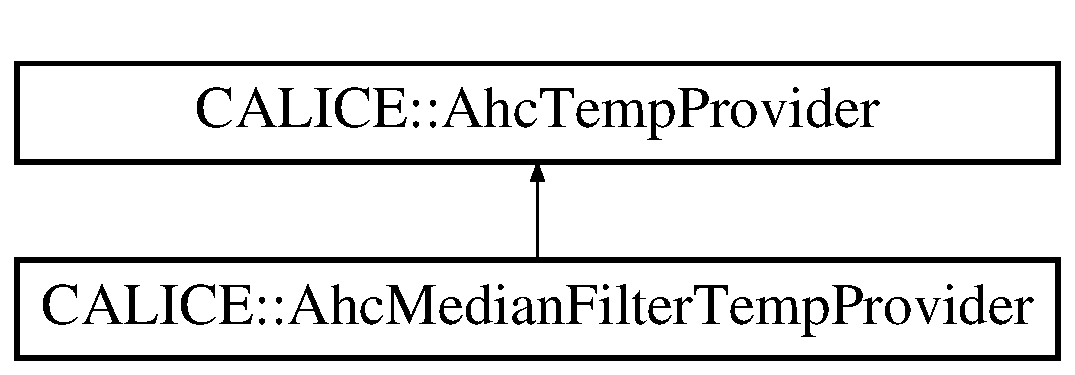
\includegraphics[height=2.000000cm]{classCALICE_1_1AhcMedianFilterTempProvider}
\end{center}
\end{figure}
\subsection*{Public Member Functions}
\begin{DoxyCompactItemize}
\item 
{\bfseries Ahc\-Median\-Filter\-Temp\-Provider} ({\bf Ahc\-Mapper} const $\ast$mapper)\label{classCALICE_1_1AhcMedianFilterTempProvider_afc6895b4468f12307c2da9f64c3eb5ed}

\item 
virtual float {\bf get\-Cell\-Temp} (int module, int chip, int chan)
\begin{DoxyCompactList}\small\item\em Returns the temperature for the cell in the specified module connected to the given chip and channel. \end{DoxyCompactList}\item 
virtual float {\bf get\-Cell\-Temp\-Error} (int module, int chip, int chan)\label{classCALICE_1_1AhcMedianFilterTempProvider_ace083f026078087a40383dd051d34843}

\begin{DoxyCompactList}\small\item\em Returns the error on the temperature for the cell in the specified module connected to the given chip and channel. \end{DoxyCompactList}\item 
virtual float {\bf get\-Avg\-Temp} ()\label{classCALICE_1_1AhcMedianFilterTempProvider_a237fba51962e5102c9580cfa9ed431fa}

\begin{DoxyCompactList}\small\item\em Returns the average calorimeter temperature. \end{DoxyCompactList}\item 
virtual float {\bf get\-Avg\-Module\-Temp} (unsigned module)\label{classCALICE_1_1AhcMedianFilterTempProvider_a5395b7d6095c39af7e0b80b133ba400d}

\begin{DoxyCompactList}\small\item\em Returns the average module temperature. \end{DoxyCompactList}\item 
float {\bf get\-Sensor\-Temp} (int module, int sensor)\label{classCALICE_1_1AhcMedianFilterTempProvider_ac9f730849a87bda3106773b7dc869f2e}

\begin{DoxyCompactList}\small\item\em Return the temperature for the specified module and sensor. \end{DoxyCompactList}\end{DoxyCompactItemize}
\subsection*{Protected Member Functions}
\begin{DoxyCompactItemize}
\item 
virtual void {\bf apply\-Correction} ()
\begin{DoxyCompactList}\small\item\em This function applies the correction to the internal 'cache' for the temperature values from the five sensors. \end{DoxyCompactList}\item 
bool {\bf is\-Bad\-Value} (float t)\label{classCALICE_1_1AhcMedianFilterTempProvider_a708c84d516d63059ba6665dae2da147e}

\begin{DoxyCompactList}\small\item\em Returns true if argument value is outside the sanity range. \end{DoxyCompactList}\end{DoxyCompactItemize}
\subsection*{Private Member Functions}
\begin{DoxyCompactItemize}
\item 
int {\bf get\-Sensor} (int chip, int chan)\label{classCALICE_1_1AhcMedianFilterTempProvider_a23a23ba36d563be88a3f1a20a51b28c9}

\begin{DoxyCompactList}\small\item\em Returns the closest sensor to cell connected to chip, chan according to D\-E\-S\-Y-\/\-T\-H\-E\-S\-I\-S-\/2008-\/050. \end{DoxyCompactList}\item 
double {\bfseries median} (float a[$\,$], int n)\label{classCALICE_1_1AhcMedianFilterTempProvider_acab9513cd7e4395371bde8d433177cdb}

\end{DoxyCompactItemize}
\subsection*{Private Attributes}
\begin{DoxyCompactItemize}
\item 
{\bf Ahc\-Mapper} const $\ast$ {\bfseries \-\_\-mapper}\label{classCALICE_1_1AhcMedianFilterTempProvider_aa401791e44b7cc8c0c9093b66d84ac6a}

\item 
float {\bfseries \-\_\-calo\-Mean\-Temp}\label{classCALICE_1_1AhcMedianFilterTempProvider_a76bfbd1b9fd6deead5eeaf572f2498ef}

\item 
float {\bfseries \-\_\-calo\-Mean\-Temp\-R\-M\-S}\label{classCALICE_1_1AhcMedianFilterTempProvider_a73f567416a0bcb8b5f8a130df8cad1f3}

\item 
int {\bfseries \-\_\-calo\-Mean\-Count}\label{classCALICE_1_1AhcMedianFilterTempProvider_abfa3e2672c774bc6814b5f44eda6ba9a}

\item 
std\-::vector$<$ float $>$ {\bfseries \-\_\-module\-Mean\-Temp}\label{classCALICE_1_1AhcMedianFilterTempProvider_a20f5463fcf3ba997a6b081615830940f}

\item 
std\-::vector$<$ float $>$ {\bfseries \-\_\-module\-Mean\-Temp\-R\-M\-S}\label{classCALICE_1_1AhcMedianFilterTempProvider_aecb3f33637742eb7af6b9e0cbdb276a8}

\item 
std\-::vector$<$ int $>$ {\bfseries \-\_\-module\-Mean\-Count}\label{classCALICE_1_1AhcMedianFilterTempProvider_a17ece36832271a1590d721aabc0ce7ed}

\end{DoxyCompactItemize}
\subsection*{Additional Inherited Members}


\subsection{Detailed Description}
This is a very simple temperature provider for the ahcal. 

What it does\-:
\begin{DoxyItemize}
\item the calibration set is applied
\item if a temperature sensor gives a value outside the defined sanity range the value is replaced by the average of the four sensors in that module
\item for each cell the temperature value from the 'closest' sensor, according to the table 3.\-1, D\-E\-S\-Y-\/\-T\-H\-E\-S\-I\-S-\/2008-\/050 is returned
\end{DoxyItemize}

Also see the documentation for the several functions for more detailed information. This new temperature provider with median filter created\-: Date\-: August 2013 Author\-: Sergey Morozov The temperature provider is based on the \doxyref{Ahc\-Simple\-Temp\-Provider}{p.}{classCALICE_1_1AhcSimpleTempProvider} with some updates\-:
\begin{DoxyItemize}
\item all temperature sensors are set to the layer average temperature.
\item the median filter to layer-\/by-\/layer profile has been introduced. This will help to remove the out-\/layers with wrong temperature measurements in some layers of A\-H\-C\-A\-L. Note\-: you need smooth (median filtered for example) M\-I\-P and gain temperature profiles in the M\-I\-P and gain calibrations to use this tempetarure provider for data reconstruction! 
\end{DoxyItemize}

Definition at line 38 of file Ahc\-Median\-Filter\-Temp\-Provider.\-hh.



\subsection{Member Function Documentation}
\index{C\-A\-L\-I\-C\-E\-::\-Ahc\-Median\-Filter\-Temp\-Provider@{C\-A\-L\-I\-C\-E\-::\-Ahc\-Median\-Filter\-Temp\-Provider}!apply\-Correction@{apply\-Correction}}
\index{apply\-Correction@{apply\-Correction}!CALICE::AhcMedianFilterTempProvider@{C\-A\-L\-I\-C\-E\-::\-Ahc\-Median\-Filter\-Temp\-Provider}}
\subsubsection[{apply\-Correction}]{\setlength{\rightskip}{0pt plus 5cm}void C\-A\-L\-I\-C\-E\-::\-Ahc\-Median\-Filter\-Temp\-Provider\-::apply\-Correction (
\begin{DoxyParamCaption}
{}
\end{DoxyParamCaption}
)\hspace{0.3cm}{\ttfamily [protected]}, {\ttfamily [virtual]}}\label{classCALICE_1_1AhcMedianFilterTempProvider_a9ffdad9db5836b0ceb55f317095cfe8c}


This function applies the correction to the internal 'cache' for the temperature values from the five sensors. 

It should be called everytime a new collection of temperatures or calibrations have been at set or the sanity range has been changed, i.\-e. if one of new\-Sro\-Mod\-Col, new\-Calib\-Col or new\-Sanity\-Range is true. This is done in \doxyref{get\-Cell\-Temp()}{p.}{classCALICE_1_1AhcMedianFilterTempProvider_a2d5865711d94a975e593df2713608880} and \doxyref{get\-Cell\-Temp\-Error()}{p.}{classCALICE_1_1AhcMedianFilterTempProvider_ace083f026078087a40383dd051d34843}. 

Definition at line 97 of file Ahc\-Median\-Filter\-Temp\-Provider.\-cc.



References C\-A\-L\-I\-C\-E\-::\-Ahc\-Temp\-Provider\-::\-\_\-sro\-Mod\-Col, C\-A\-L\-I\-C\-E\-::\-Ahc\-Mapper\-::get\-K(), C\-A\-L\-I\-C\-E\-::\-Scint\-Calo\-Slow\-Readout\-Mod\-Block\-::get\-Module\-Number(), is\-Bad\-Value(), C\-A\-L\-I\-C\-E\-::\-Ahc\-Temp\-Provider\-::new\-Calib\-Col, C\-A\-L\-I\-C\-E\-::\-Ahc\-Temp\-Provider\-::new\-Sanity\-Range, C\-A\-L\-I\-C\-E\-::\-Ahc\-Temp\-Provider\-::new\-Sro\-Mod\-Col, C\-A\-L\-I\-C\-E\-::\-Ahc\-Temp\-Provider\-::sensor\-Temp, C\-A\-L\-I\-C\-E\-::\-Ahc\-Temp\-Provider\-::sensor\-Temp\-Error, and C\-A\-L\-I\-C\-E\-::\-Ahc\-Temp\-Provider\-::update\-Cache().



Referenced by get\-Avg\-Module\-Temp(), get\-Avg\-Temp(), get\-Cell\-Temp(), get\-Cell\-Temp\-Error(), and get\-Sensor\-Temp().

\index{C\-A\-L\-I\-C\-E\-::\-Ahc\-Median\-Filter\-Temp\-Provider@{C\-A\-L\-I\-C\-E\-::\-Ahc\-Median\-Filter\-Temp\-Provider}!get\-Cell\-Temp@{get\-Cell\-Temp}}
\index{get\-Cell\-Temp@{get\-Cell\-Temp}!CALICE::AhcMedianFilterTempProvider@{C\-A\-L\-I\-C\-E\-::\-Ahc\-Median\-Filter\-Temp\-Provider}}
\subsubsection[{get\-Cell\-Temp}]{\setlength{\rightskip}{0pt plus 5cm}float C\-A\-L\-I\-C\-E\-::\-Ahc\-Median\-Filter\-Temp\-Provider\-::get\-Cell\-Temp (
\begin{DoxyParamCaption}
\item[{int}]{module, }
\item[{int}]{chip, }
\item[{int}]{chan}
\end{DoxyParamCaption}
)\hspace{0.3cm}{\ttfamily [virtual]}}\label{classCALICE_1_1AhcMedianFilterTempProvider_a2d5865711d94a975e593df2713608880}


Returns the temperature for the cell in the specified module connected to the given chip and channel. 

For each cell the temperature value from the 'closest' sensor, according to the table 3.\-1, D\-E\-S\-Y-\/\-T\-H\-E\-S\-I\-S-\/2008-\/050 is returned. 

Implements {\bf C\-A\-L\-I\-C\-E\-::\-Ahc\-Temp\-Provider} \doxyref{}{p.}{classCALICE_1_1AhcTempProvider_aa12c75d45d7ade54316dd113a6bab2d1}.



Definition at line 19 of file Ahc\-Median\-Filter\-Temp\-Provider.\-cc.



References apply\-Correction(), get\-Sensor(), C\-A\-L\-I\-C\-E\-::\-Ahc\-Temp\-Provider\-::new\-Calib\-Col, C\-A\-L\-I\-C\-E\-::\-Ahc\-Temp\-Provider\-::new\-Sanity\-Range, C\-A\-L\-I\-C\-E\-::\-Ahc\-Temp\-Provider\-::new\-Sro\-Mod\-Col, and C\-A\-L\-I\-C\-E\-::\-Ahc\-Temp\-Provider\-::sensor\-Temp.



The documentation for this class was generated from the following files\-:\begin{DoxyCompactItemize}
\item 
Ahc\-Median\-Filter\-Temp\-Provider.\-hh\item 
Ahc\-Median\-Filter\-Temp\-Provider.\-cc\end{DoxyCompactItemize}

\section{C\-A\-L\-I\-C\-E\-:\-:Ahc\-Simple\-Temp\-Provider Class Reference}
\label{classCALICE_1_1AhcSimpleTempProvider}\index{C\-A\-L\-I\-C\-E\-::\-Ahc\-Simple\-Temp\-Provider@{C\-A\-L\-I\-C\-E\-::\-Ahc\-Simple\-Temp\-Provider}}


This is a very simple temperature provider for the ahcal.  




{\ttfamily \#include $<$Ahc\-Simple\-Temp\-Provider.\-hh$>$}

Inheritance diagram for C\-A\-L\-I\-C\-E\-:\-:Ahc\-Simple\-Temp\-Provider\-:\begin{figure}[H]
\begin{center}
\leavevmode
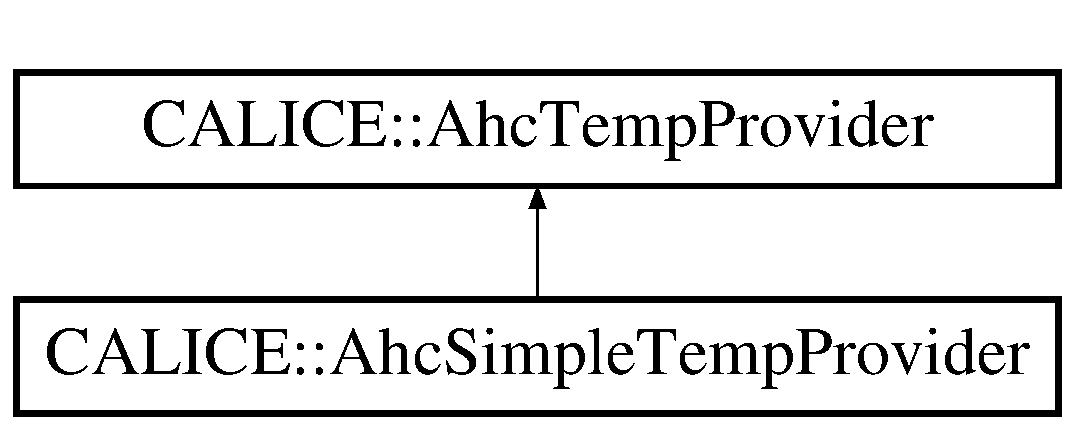
\includegraphics[height=2.000000cm]{classCALICE_1_1AhcSimpleTempProvider}
\end{center}
\end{figure}
\subsection*{Public Member Functions}
\begin{DoxyCompactItemize}
\item 
virtual float {\bf get\-Cell\-Temp} (int module, int chip, int chan)
\begin{DoxyCompactList}\small\item\em Returns the temperature for the cell in the specified module connected to the given chip and channel. \end{DoxyCompactList}\item 
virtual float {\bf get\-Cell\-Temp\-Error} (int module, int chip, int chan)\label{classCALICE_1_1AhcSimpleTempProvider_a2d3cd7fd1a3f144f62991e39b44d016f}

\begin{DoxyCompactList}\small\item\em Returns the error on the temperature for the cell in the specified module connected to the given chip and channel. \end{DoxyCompactList}\item 
virtual float {\bf get\-Avg\-Temp} ()\label{classCALICE_1_1AhcSimpleTempProvider_ae2055a46cab875cb672f33bf6395b3b7}

\begin{DoxyCompactList}\small\item\em Returns the average calorimeter temperature. \end{DoxyCompactList}\item 
virtual float {\bf get\-Avg\-Module\-Temp} (unsigned module)\label{classCALICE_1_1AhcSimpleTempProvider_abff6b07a15d952dc1f90a6e41500dabc}

\begin{DoxyCompactList}\small\item\em Returns the average module temperature. \end{DoxyCompactList}\item 
float {\bf get\-Sensor\-Temp} (int module, int sensor)\label{classCALICE_1_1AhcSimpleTempProvider_ab61d13863930498a336476d9ac049b2e}

\begin{DoxyCompactList}\small\item\em Return the temperature for the specified module and sensor. \end{DoxyCompactList}\end{DoxyCompactItemize}
\subsection*{Protected Member Functions}
\begin{DoxyCompactItemize}
\item 
virtual void {\bf apply\-Correction} ()
\begin{DoxyCompactList}\small\item\em This function applies the correction to the internal 'cache' for the temperature values from the five sensors. \end{DoxyCompactList}\item 
bool {\bf is\-Bad\-Value} (float t)\label{classCALICE_1_1AhcSimpleTempProvider_ab3f94a954ed71d269997f0b2cde87941}

\begin{DoxyCompactList}\small\item\em Returns true if argument value is outside the sanity range. \end{DoxyCompactList}\end{DoxyCompactItemize}
\subsection*{Private Member Functions}
\begin{DoxyCompactItemize}
\item 
int {\bf get\-Sensor} (int chip, int chan)\label{classCALICE_1_1AhcSimpleTempProvider_ad000dcb24a383043a9c72b93d2f05836}

\begin{DoxyCompactList}\small\item\em Returns the closest sensor to cell connected to chip, chan according to D\-E\-S\-Y-\/\-T\-H\-E\-S\-I\-S-\/2008-\/050. \end{DoxyCompactList}\end{DoxyCompactItemize}
\subsection*{Private Attributes}
\begin{DoxyCompactItemize}
\item 
float {\bfseries \-\_\-calo\-Mean\-Temp}\label{classCALICE_1_1AhcSimpleTempProvider_a254fa40b19cdc8b1c09a04b201afff2f}

\item 
float {\bfseries \-\_\-calo\-Mean\-Temp\-R\-M\-S}\label{classCALICE_1_1AhcSimpleTempProvider_abe15d788019a2a354f8060dbfb9ef6e3}

\item 
int {\bfseries \-\_\-calo\-Mean\-Count}\label{classCALICE_1_1AhcSimpleTempProvider_a25cd84b21c382d4b7a2fc377588244b9}

\item 
std\-::vector$<$ float $>$ {\bfseries \-\_\-module\-Mean\-Temp}\label{classCALICE_1_1AhcSimpleTempProvider_a4d9109bd33c31ae2b06497ff73aeeb6e}

\item 
std\-::vector$<$ float $>$ {\bfseries \-\_\-module\-Mean\-Temp\-R\-M\-S}\label{classCALICE_1_1AhcSimpleTempProvider_a7573f43d01d8a5563367f15527ed711e}

\item 
std\-::vector$<$ int $>$ {\bfseries \-\_\-module\-Mean\-Count}\label{classCALICE_1_1AhcSimpleTempProvider_ad3c12b5824a629e59d8dcc4ff4869684}

\end{DoxyCompactItemize}
\subsection*{Additional Inherited Members}


\subsection{Detailed Description}
This is a very simple temperature provider for the ahcal. 

What it does\-:
\begin{DoxyItemize}
\item the calibration set is applied
\item if a temperature sensor gives a value outside the defined sanity range the value is replaced by the average of the four sensors in that module
\item for each cell the temperature value from the 'closest' sensor, according to the table 3.\-1, D\-E\-S\-Y-\/\-T\-H\-E\-S\-I\-S-\/2008-\/050 is returned
\end{DoxyItemize}

Also see the documentation for the several functions for more detailed information. 

Definition at line 25 of file Ahc\-Simple\-Temp\-Provider.\-hh.



\subsection{Member Function Documentation}
\index{C\-A\-L\-I\-C\-E\-::\-Ahc\-Simple\-Temp\-Provider@{C\-A\-L\-I\-C\-E\-::\-Ahc\-Simple\-Temp\-Provider}!apply\-Correction@{apply\-Correction}}
\index{apply\-Correction@{apply\-Correction}!CALICE::AhcSimpleTempProvider@{C\-A\-L\-I\-C\-E\-::\-Ahc\-Simple\-Temp\-Provider}}
\subsubsection[{apply\-Correction}]{\setlength{\rightskip}{0pt plus 5cm}void C\-A\-L\-I\-C\-E\-::\-Ahc\-Simple\-Temp\-Provider\-::apply\-Correction (
\begin{DoxyParamCaption}
{}
\end{DoxyParamCaption}
)\hspace{0.3cm}{\ttfamily [protected]}, {\ttfamily [virtual]}}\label{classCALICE_1_1AhcSimpleTempProvider_a465f433cd5082a1c3224262e179604e1}


This function applies the correction to the internal 'cache' for the temperature values from the five sensors. 

It should be called everytime a new collection of temperatures or calibrations have been at set or the sanity range has been changed, i.\-e. if one of new\-Sro\-Mod\-Col, new\-Calib\-Col or new\-Sanity\-Range is true. This is done in \doxyref{get\-Cell\-Temp()}{p.}{classCALICE_1_1AhcSimpleTempProvider_aff9186dfdab4801e41540f1d63428e3f} and \doxyref{get\-Cell\-Temp\-Error()}{p.}{classCALICE_1_1AhcSimpleTempProvider_a2d3cd7fd1a3f144f62991e39b44d016f}. 

Definition at line 82 of file Ahc\-Simple\-Temp\-Provider.\-cc.



References C\-A\-L\-I\-C\-E\-::\-Ahc\-Temp\-Provider\-::\-\_\-sro\-Mod\-Col, C\-A\-L\-I\-C\-E\-::\-Scint\-Calo\-Slow\-Readout\-Mod\-Block\-::get\-Module\-Number(), is\-Bad\-Value(), C\-A\-L\-I\-C\-E\-::\-Ahc\-Temp\-Provider\-::new\-Calib\-Col, C\-A\-L\-I\-C\-E\-::\-Ahc\-Temp\-Provider\-::new\-Sanity\-Range, C\-A\-L\-I\-C\-E\-::\-Ahc\-Temp\-Provider\-::new\-Sro\-Mod\-Col, C\-A\-L\-I\-C\-E\-::\-Ahc\-Temp\-Provider\-::sensor\-Temp, C\-A\-L\-I\-C\-E\-::\-Ahc\-Temp\-Provider\-::sensor\-Temp\-Error, and C\-A\-L\-I\-C\-E\-::\-Ahc\-Temp\-Provider\-::update\-Cache().



Referenced by get\-Avg\-Module\-Temp(), get\-Avg\-Temp(), get\-Cell\-Temp(), get\-Cell\-Temp\-Error(), and get\-Sensor\-Temp().

\index{C\-A\-L\-I\-C\-E\-::\-Ahc\-Simple\-Temp\-Provider@{C\-A\-L\-I\-C\-E\-::\-Ahc\-Simple\-Temp\-Provider}!get\-Cell\-Temp@{get\-Cell\-Temp}}
\index{get\-Cell\-Temp@{get\-Cell\-Temp}!CALICE::AhcSimpleTempProvider@{C\-A\-L\-I\-C\-E\-::\-Ahc\-Simple\-Temp\-Provider}}
\subsubsection[{get\-Cell\-Temp}]{\setlength{\rightskip}{0pt plus 5cm}float C\-A\-L\-I\-C\-E\-::\-Ahc\-Simple\-Temp\-Provider\-::get\-Cell\-Temp (
\begin{DoxyParamCaption}
\item[{int}]{module, }
\item[{int}]{chip, }
\item[{int}]{chan}
\end{DoxyParamCaption}
)\hspace{0.3cm}{\ttfamily [virtual]}}\label{classCALICE_1_1AhcSimpleTempProvider_aff9186dfdab4801e41540f1d63428e3f}


Returns the temperature for the cell in the specified module connected to the given chip and channel. 

For each cell the temperature value from the 'closest' sensor, according to the table 3.\-1, D\-E\-S\-Y-\/\-T\-H\-E\-S\-I\-S-\/2008-\/050 is returned. 

Implements {\bf C\-A\-L\-I\-C\-E\-::\-Ahc\-Temp\-Provider} \doxyref{}{p.}{classCALICE_1_1AhcTempProvider_aa12c75d45d7ade54316dd113a6bab2d1}.



Definition at line 6 of file Ahc\-Simple\-Temp\-Provider.\-cc.



References apply\-Correction(), get\-Sensor(), C\-A\-L\-I\-C\-E\-::\-Ahc\-Temp\-Provider\-::new\-Calib\-Col, C\-A\-L\-I\-C\-E\-::\-Ahc\-Temp\-Provider\-::new\-Sanity\-Range, C\-A\-L\-I\-C\-E\-::\-Ahc\-Temp\-Provider\-::new\-Sro\-Mod\-Col, and C\-A\-L\-I\-C\-E\-::\-Ahc\-Temp\-Provider\-::sensor\-Temp.



The documentation for this class was generated from the following files\-:\begin{DoxyCompactItemize}
\item 
Ahc\-Simple\-Temp\-Provider.\-hh\item 
Ahc\-Simple\-Temp\-Provider.\-cc\end{DoxyCompactItemize}

\section{C\-A\-L\-I\-C\-E\-:\-:Ahc\-Slow\-Readout\-Block Class Reference}
\label{classCALICE_1_1AhcSlowReadoutBlock}\index{C\-A\-L\-I\-C\-E\-::\-Ahc\-Slow\-Readout\-Block@{C\-A\-L\-I\-C\-E\-::\-Ahc\-Slow\-Readout\-Block}}


Interface Class to access the Ahc\-Slow\-Configuration Data For the time being we treat only the movable stage positions Update\-: 6/7/08 Added z and rotated position of stage (Maintain backward compatibility)  




{\ttfamily \#include $<$Ahc\-Slow\-Readout\-Block.\-hh$>$}

Inheritance diagram for C\-A\-L\-I\-C\-E\-:\-:Ahc\-Slow\-Readout\-Block\-:\begin{figure}[H]
\begin{center}
\leavevmode
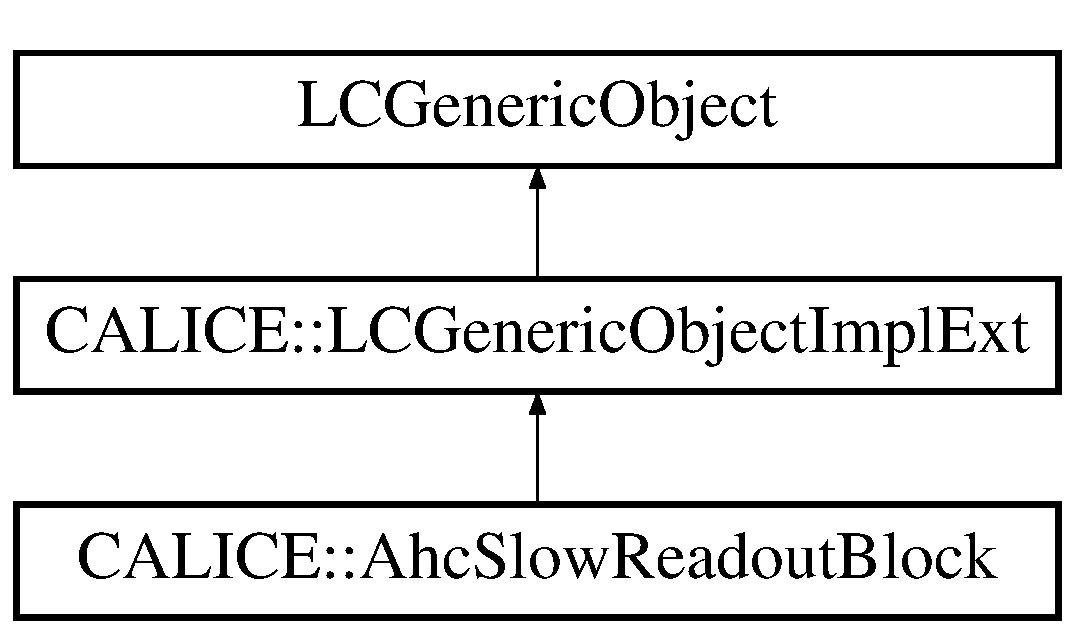
\includegraphics[height=3.000000cm]{classCALICE_1_1AhcSlowReadoutBlock}
\end{center}
\end{figure}
\subsection*{Public Member Functions}
\begin{DoxyCompactItemize}
\item 
{\bf Ahc\-Slow\-Readout\-Block} ()\label{classCALICE_1_1AhcSlowReadoutBlock_a5cdefa13a9db415369ef3df6e3b39da8}

\begin{DoxyCompactList}\small\item\em Simple Constructor. \end{DoxyCompactList}\item 
{\bf Ahc\-Slow\-Readout\-Block} (L\-C\-Object $\ast${\bf obj})\label{classCALICE_1_1AhcSlowReadoutBlock_a5b753db9f7e51e90eb67ca16e053faac}

\begin{DoxyCompactList}\small\item\em 'Copy constructor' needed to interpret L\-C\-Collection read from file/database. \end{DoxyCompactList}\item 
{\bf Ahc\-Slow\-Readout\-Block} \& {\bfseries set\-\_\-xyz\-Position\-\_\-mm} (double xpos, double ypos, double zpos)\label{classCALICE_1_1AhcSlowReadoutBlock_a07a5a75c46e30d25d87c46d5cf8dba73}

\item 
{\bf Ahc\-Slow\-Readout\-Block} \& {\bfseries set\-\_\-rot\-Position\-\_\-deg} (double cpos)\label{classCALICE_1_1AhcSlowReadoutBlock_aa4a13bec9f6c5db71c8cf3b793c08709}

\item 
virtual double {\bfseries get\-\_\-x\-Position\-\_\-mm} ()\label{classCALICE_1_1AhcSlowReadoutBlock_a62d5383dfd433dc6eebbd38abd1f8a7c}

\item 
virtual double {\bfseries get\-\_\-y\-Position\-\_\-mm} ()\label{classCALICE_1_1AhcSlowReadoutBlock_a59c904fd485befa6d9afe0cd2424ab20}

\item 
virtual double {\bfseries get\-\_\-z\-Position\-\_\-mm} ()\label{classCALICE_1_1AhcSlowReadoutBlock_a73203222645101c2b8ce65736bf7752f}

\item 
virtual double {\bfseries get\-\_\-c\-Position\-\_\-deg} ()\label{classCALICE_1_1AhcSlowReadoutBlock_add5f7179047770f32f533ac660612b1d}

\item 
void {\bf print} (std\-::ostream \&os)\label{classCALICE_1_1AhcSlowReadoutBlock_a4133b32c50c5946b39da0f961811f09a}

\begin{DoxyCompactList}\small\item\em Convenient print method. \end{DoxyCompactList}\item 
const std\-::string {\bf get\-Type\-Name} () const \label{classCALICE_1_1AhcSlowReadoutBlock_ae8699367e40866501f179e740a80bcab}

\begin{DoxyCompactList}\small\item\em Return the type of the class. \end{DoxyCompactList}\item 
const std\-::string {\bf get\-Data\-Description} () const \label{classCALICE_1_1AhcSlowReadoutBlock_ae057949d71e0d6d7f4f2a808222b683c}

\begin{DoxyCompactList}\small\item\em Return a brief description of the data members. \end{DoxyCompactList}\end{DoxyCompactItemize}
\subsection*{Additional Inherited Members}


\subsection{Detailed Description}
Interface Class to access the Ahc\-Slow\-Configuration Data For the time being we treat only the movable stage positions Update\-: 6/7/08 Added z and rotated position of stage (Maintain backward compatibility) 

\begin{DoxyAuthor}{Author}
\-: Roman P�schl D\-E\-S\-Y 
\end{DoxyAuthor}
\begin{DoxyDate}{Date}
Nov 2005 
\end{DoxyDate}


Definition at line 28 of file Ahc\-Slow\-Readout\-Block.\-hh.



The documentation for this class was generated from the following files\-:\begin{DoxyCompactItemize}
\item 
Ahc\-Slow\-Readout\-Block.\-hh\item 
Ahc\-Slow\-Readout\-Block.\-cc\end{DoxyCompactItemize}

\section{C\-A\-L\-I\-C\-E\-:\-:Ahc\-Slow\-Readout\-Mod\-Block Class Reference}
\label{classCALICE_1_1AhcSlowReadoutModBlock}\index{C\-A\-L\-I\-C\-E\-::\-Ahc\-Slow\-Readout\-Mod\-Block@{C\-A\-L\-I\-C\-E\-::\-Ahc\-Slow\-Readout\-Mod\-Block}}


Interface Class to access the Ahc\-Slow\-Readout Data Here we handle ahc voltages, temperatures et al.  




{\ttfamily \#include $<$Ahc\-Slow\-Readout\-Mod\-Block.\-hh$>$}

Inheritance diagram for C\-A\-L\-I\-C\-E\-:\-:Ahc\-Slow\-Readout\-Mod\-Block\-:\begin{figure}[H]
\begin{center}
\leavevmode
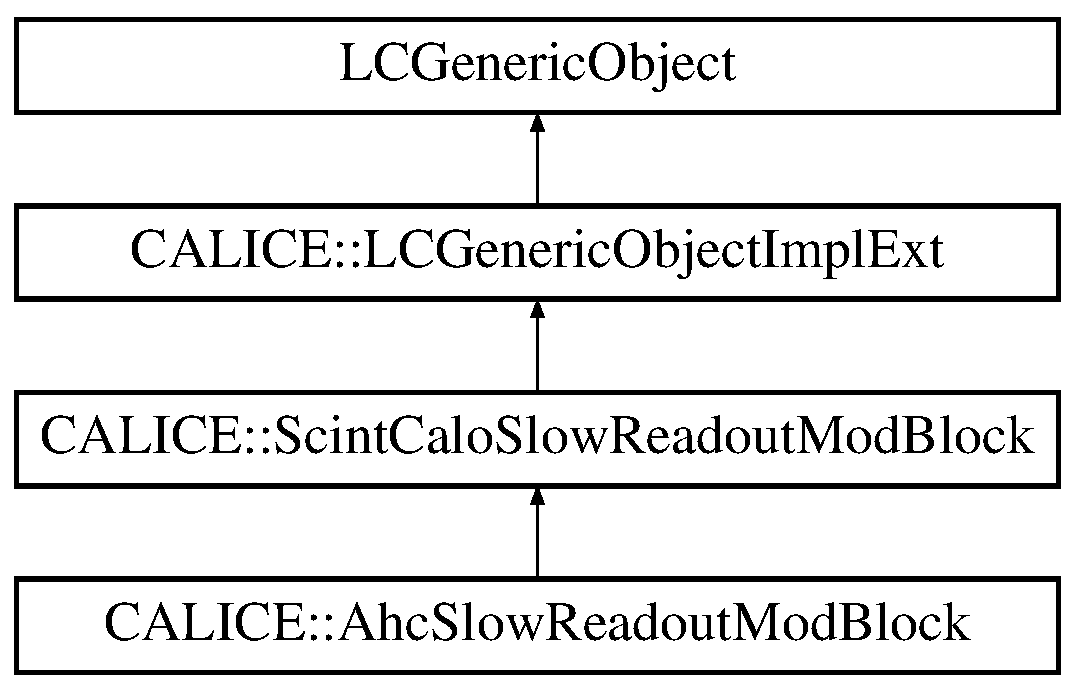
\includegraphics[height=4.000000cm]{classCALICE_1_1AhcSlowReadoutModBlock}
\end{center}
\end{figure}
\subsection*{Public Member Functions}
\begin{DoxyCompactItemize}
\item 
{\bf Ahc\-Slow\-Readout\-Mod\-Block} ()\label{classCALICE_1_1AhcSlowReadoutModBlock_a78919030cda78f1b40731c8124a28eac}

\begin{DoxyCompactList}\small\item\em Constructor. \end{DoxyCompactList}\item 
{\bf Ahc\-Slow\-Readout\-Mod\-Block} (L\-C\-Object $\ast${\bf obj})\label{classCALICE_1_1AhcSlowReadoutModBlock_a9a979a604c82e966f9a30ae3b55971ac}

\begin{DoxyCompactList}\small\item\em 'Copy constructor' needed to interpret L\-C\-Collection read from file/database. \end{DoxyCompactList}\item 
std\-::vector$<$ double $>$ \& {\bf get\-Cmb\-Values} ()\label{classCALICE_1_1AhcSlowReadoutModBlock_aac2c55bb18e8ca946d12c227de07d9a7}

\begin{DoxyCompactList}\small\item\em Retrieve the cmb values. \end{DoxyCompactList}\item 
std\-::vector$<$ double $>$ \& {\bf get\-Hbab\-Temperatures} ()\label{classCALICE_1_1AhcSlowReadoutModBlock_aad610827ad3485169aa9706cbc7128bb}

\begin{DoxyCompactList}\small\item\em Retrieve the hbab temperatures. \end{DoxyCompactList}\item 
void {\bf print} (std\-::ostream \&)
\begin{DoxyCompactList}\small\item\em convenient print method \end{DoxyCompactList}\item 
virtual const std\-::string {\bf get\-Type\-Name} () const \label{classCALICE_1_1AhcSlowReadoutModBlock_a0dc8e7472edb78736a8d740dab998e23}

\begin{DoxyCompactList}\small\item\em Return the type of the class. \end{DoxyCompactList}\item 
virtual const std\-::string {\bf get\-Data\-Description} () const \label{classCALICE_1_1AhcSlowReadoutModBlock_a8343c0f0c11517815ec3c9279cb63000}

\begin{DoxyCompactList}\small\item\em Return a brief description of the data members. \end{DoxyCompactList}\end{DoxyCompactItemize}
\subsection*{Private Member Functions}
\begin{DoxyCompactItemize}
\item 
void {\bf set\-Types} ()\label{classCALICE_1_1AhcSlowReadoutModBlock_a4b22eb001e649f486a88bfddb2c1ed68}

\begin{DoxyCompactList}\small\item\em This method defines the (general) types of the measured values A type not present here will not be handled!!! \end{DoxyCompactList}\end{DoxyCompactItemize}
\subsection*{Private Attributes}
\begin{DoxyCompactItemize}
\item 
std\-::vector$<$ double $>$ {\bf \-\_\-cmb\-Values}
\begin{DoxyCompactList}\small\item\em The output vectors. \end{DoxyCompactList}\item 
std\-::vector$<$ double $>$ {\bf \-\_\-hbab\-Temperatures}\label{classCALICE_1_1AhcSlowReadoutModBlock_aedce23ae2abcf8741fd34ecc5d7a7e60}

\begin{DoxyCompactList}\small\item\em hbab temperatures \end{DoxyCompactList}\end{DoxyCompactItemize}
\subsection*{Additional Inherited Members}


\subsection{Detailed Description}
Interface Class to access the Ahc\-Slow\-Readout Data Here we handle ahc voltages, temperatures et al. 

when filling the class the string identifying the measured values has to be given first, a warning is issued if no identifier is given for a given datatype. On the other hand this concerns just the filler of the class, i.\-e. the conversion where it is done once for all. See the print method at the end of the class for the meaning of the fields (as of 31/7/06) Use the interface methods to retrieve the data fields \begin{DoxyAuthor}{Author}
Roman P�schl L\-A\-L/\-Orsay 
\end{DoxyAuthor}
\begin{DoxyDate}{Date}
Aug 2006 
\end{DoxyDate}


Definition at line 56 of file Ahc\-Slow\-Readout\-Mod\-Block.\-hh.



\subsection{Member Function Documentation}
\index{C\-A\-L\-I\-C\-E\-::\-Ahc\-Slow\-Readout\-Mod\-Block@{C\-A\-L\-I\-C\-E\-::\-Ahc\-Slow\-Readout\-Mod\-Block}!print@{print}}
\index{print@{print}!CALICE::AhcSlowReadoutModBlock@{C\-A\-L\-I\-C\-E\-::\-Ahc\-Slow\-Readout\-Mod\-Block}}
\subsubsection[{print}]{\setlength{\rightskip}{0pt plus 5cm}void C\-A\-L\-I\-C\-E\-::\-Ahc\-Slow\-Readout\-Mod\-Block\-::print (
\begin{DoxyParamCaption}
\item[{std\-::ostream \&}]{os}
\end{DoxyParamCaption}
)}\label{classCALICE_1_1AhcSlowReadoutModBlock_a697eeaf3c34576c3c4541bdc3fcd35c2}


convenient print method 

Convenient print method. 

Definition at line 33 of file Ahc\-Slow\-Readout\-Mod\-Block.\-cc.



References C\-A\-L\-I\-C\-E\-::\-Scint\-Calo\-Slow\-Readout\-Mod\-Block\-::\-\_\-hbab\-Voltages, C\-A\-L\-I\-C\-E\-::\-Scint\-Calo\-Slow\-Readout\-Mod\-Block\-::get\-Cmb\-Height(), C\-A\-L\-I\-C\-E\-::\-Scint\-Calo\-Slow\-Readout\-Mod\-Block\-::get\-Cmb\-Temperatures(), get\-Cmb\-Values(), C\-A\-L\-I\-C\-E\-::\-Scint\-Calo\-Slow\-Readout\-Mod\-Block\-::get\-Cmb\-Voltages(), C\-A\-L\-I\-C\-E\-::\-Scint\-Calo\-Slow\-Readout\-Mod\-Block\-::get\-Cmb\-Width(), get\-Hbab\-Temperatures(), C\-A\-L\-I\-C\-E\-::\-Scint\-Calo\-Slow\-Readout\-Mod\-Block\-::get\-Hbab\-Voltages(), C\-A\-L\-I\-C\-E\-::\-Scint\-Calo\-Slow\-Readout\-Mod\-Block\-::get\-Led\-Setting(), C\-A\-L\-I\-C\-E\-::\-Scint\-Calo\-Slow\-Readout\-Mod\-Block\-::get\-Module\-Number(), C\-A\-L\-I\-C\-E\-::\-Scint\-Calo\-Slow\-Readout\-Mod\-Block\-::get\-Time\-Stamp(), C\-A\-L\-I\-C\-E\-::\-Scint\-Calo\-Slow\-Readout\-Mod\-Block\-::prepare\-Output\-Vecs(), and C\-A\-L\-I\-C\-E\-::to\-\_\-binary\-\_\-bitops().



\subsection{Field Documentation}
\index{C\-A\-L\-I\-C\-E\-::\-Ahc\-Slow\-Readout\-Mod\-Block@{C\-A\-L\-I\-C\-E\-::\-Ahc\-Slow\-Readout\-Mod\-Block}!\-\_\-cmb\-Values@{\-\_\-cmb\-Values}}
\index{\-\_\-cmb\-Values@{\-\_\-cmb\-Values}!CALICE::AhcSlowReadoutModBlock@{C\-A\-L\-I\-C\-E\-::\-Ahc\-Slow\-Readout\-Mod\-Block}}
\subsubsection[{\-\_\-cmb\-Values}]{\setlength{\rightskip}{0pt plus 5cm}std\-::vector$<$double$>$ C\-A\-L\-I\-C\-E\-::\-Ahc\-Slow\-Readout\-Mod\-Block\-::\-\_\-cmb\-Values\hspace{0.3cm}{\ttfamily [private]}}\label{classCALICE_1_1AhcSlowReadoutModBlock_a99517926e9ee2d071d74bfab855dfca8}


The output vectors. 

cmb values 

Definition at line 120 of file Ahc\-Slow\-Readout\-Mod\-Block.\-hh.



Referenced by set\-Types().



The documentation for this class was generated from the following files\-:\begin{DoxyCompactItemize}
\item 
Ahc\-Slow\-Readout\-Mod\-Block.\-hh\item 
Ahc\-Slow\-Readout\-Mod\-Block.\-cc\end{DoxyCompactItemize}

\section{C\-A\-L\-I\-C\-E\-:\-:Ahc\-Slow\-Readout\-Mod\-Mapper Class Reference}
\label{classCALICE_1_1AhcSlowReadoutModMapper}\index{C\-A\-L\-I\-C\-E\-::\-Ahc\-Slow\-Readout\-Mod\-Mapper@{C\-A\-L\-I\-C\-E\-::\-Ahc\-Slow\-Readout\-Mod\-Mapper}}


Class to correct the mapping of Ahc\-Slow\-Readout\-Mod\-Block-\/classes.  




{\ttfamily \#include $<$Ahc\-Slow\-Readout\-Mod\-Mapper.\-hh$>$}

\subsection*{Public Member Functions}
\begin{DoxyCompactItemize}
\item 
lcio\-::\-L\-C\-Collection $\ast$ {\bf map\-Collection} (const lcio\-::\-L\-C\-Collection $\ast$const col) const 
\begin{DoxyCompactList}\small\item\em returns collection with corrected Ahc\-Slow\-Readout\-Mod\-Block-\/elements for an unmapped collection of \doxyref{Ahc\-Slow\-Readout\-Mod\-Block}{p.}{classCALICE_1_1AhcSlowReadoutModBlock} \end{DoxyCompactList}\item 
void {\bf update\-Mapping} (const lcio\-::\-L\-C\-Collection $\ast$const col)
\begin{DoxyCompactList}\small\item\em Function to update the mapping. \end{DoxyCompactList}\end{DoxyCompactItemize}
\subsection*{Private Member Functions}
\begin{DoxyCompactItemize}
\item 
void {\bfseries init} ()\label{classCALICE_1_1AhcSlowReadoutModMapper_acdefd374a029f03e44e43ae651bc16fb}

\item 
void {\bfseries ensure\-Size} (unsigned int i)\label{classCALICE_1_1AhcSlowReadoutModMapper_a840d2c17a25ecfe401031047dbdf00b8}

\item 
bool {\bfseries is\-Available} (int module)\label{classCALICE_1_1AhcSlowReadoutModMapper_a8e06c12f239c65287643281ef986473d}

\item 
void {\bfseries set\-Values} ({\bf Ahc\-Slow\-Readout\-Mod\-Block} $\ast$output, const std\-::vector$<$ {\bf Ahc\-Slow\-Readout\-Mod\-Block} $\ast$ $>$ \&input, unsigned int module) const \label{classCALICE_1_1AhcSlowReadoutModMapper_a7ed1bd5cad8c574ed031c2d7ecc680aa}

\end{DoxyCompactItemize}
\subsection*{Private Attributes}
\begin{DoxyCompactItemize}
\item 
std\-::vector$<$ bool $>$ {\bfseries \-\_\-is\-Available}\label{classCALICE_1_1AhcSlowReadoutModMapper_a9c7cdd3f7492a7dcf9ce358a41d4e3a7}

\item 
std\-::vector$<$ int $>$ {\bfseries \-\_\-\-C\-M\-Blabel}\label{classCALICE_1_1AhcSlowReadoutModMapper_ae8b8700496f48a1e9056ec4ddd92abe7}

\item 
std\-::vector$<$ int $>$ {\bfseries \-\_\-\-H\-Vlabel}\label{classCALICE_1_1AhcSlowReadoutModMapper_a1ad249bcd18e4ced012b5269671810ae}

\item 
std\-::vector$<$ int $>$ {\bfseries \-\_\-\-L\-Vlabel}\label{classCALICE_1_1AhcSlowReadoutModMapper_a168f8dcf17583bc6e49b671c7824fcf7}

\end{DoxyCompactItemize}


\subsection{Detailed Description}
Class to correct the mapping of Ahc\-Slow\-Readout\-Mod\-Block-\/classes. 

The class \doxyref{Ahc\-Slow\-Readout\-Mod\-Block}{p.}{classCALICE_1_1AhcSlowReadoutModBlock} containes the module number for which the records stands. Due to problems in the slow control in the years 2006 and 2007 the values from the different data sources have been written with wrong module number. Therefore, the single \doxyref{Ahc\-Slow\-Readout\-Mod\-Block}{p.}{classCALICE_1_1AhcSlowReadoutModBlock} contains a collection of values from different modules. e.\-g. record with label \char`\"{}module = 17\char`\"{} contains C\-M\-B readings from module 23, H\-V readings from module 19 and corrupted L\-V readings

This class collects, as far as possible, the datas for the modules from the different records these ended up. If the mapping for one part is missing the values for this source will not be filled.

\begin{DoxySeeAlso}{See Also}
\doxyref{Ahc\-Slow\-Readout\-Mod\-Block}{p.}{classCALICE_1_1AhcSlowReadoutModBlock} 

\doxyref{Ahc\-Slow\-Readout\-Mod\-Mapping}{p.}{classCALICE_1_1AhcSlowReadoutModMapping}
\end{DoxySeeAlso}
\begin{DoxyAuthor}{Author}
{\tt Benjamin.\-Lutz@desy.\-de} 
\end{DoxyAuthor}
\begin{DoxyDate}{Date}
Nov 2008 
\end{DoxyDate}
\begin{DoxyVersion}{Version}
1.\-0 
\end{DoxyVersion}


Definition at line 34 of file Ahc\-Slow\-Readout\-Mod\-Mapper.\-hh.



\subsection{Member Function Documentation}
\index{C\-A\-L\-I\-C\-E\-::\-Ahc\-Slow\-Readout\-Mod\-Mapper@{C\-A\-L\-I\-C\-E\-::\-Ahc\-Slow\-Readout\-Mod\-Mapper}!map\-Collection@{map\-Collection}}
\index{map\-Collection@{map\-Collection}!CALICE::AhcSlowReadoutModMapper@{C\-A\-L\-I\-C\-E\-::\-Ahc\-Slow\-Readout\-Mod\-Mapper}}
\subsubsection[{map\-Collection}]{\setlength{\rightskip}{0pt plus 5cm}lcio\-::\-L\-C\-Collection $\ast$ C\-A\-L\-I\-C\-E\-::\-Ahc\-Slow\-Readout\-Mod\-Mapper\-::map\-Collection (
\begin{DoxyParamCaption}
\item[{const lcio\-::\-L\-C\-Collection $\ast$const}]{col}
\end{DoxyParamCaption}
) const}\label{classCALICE_1_1AhcSlowReadoutModMapper_aaf98120ee4080f6de37b5017ea6e4bb1}


returns collection with corrected Ahc\-Slow\-Readout\-Mod\-Block-\/elements for an unmapped collection of \doxyref{Ahc\-Slow\-Readout\-Mod\-Block}{p.}{classCALICE_1_1AhcSlowReadoutModBlock} 


\begin{DoxyExceptions}{Exceptions}
{\em \doxyref{Wrong\-Data\-Format\-Exception}{p.}{classCALICE_1_1WrongDataFormatException}} & When the collection type is not L\-C\-Generic\-Objects or the collection parameter \char`\"{}\-Type\-Name\char`\"{} is not \char`\"{}\-Ahc\-Slow\-Readout\-Mod\-Block\char`\"{} \\
\hline
\end{DoxyExceptions}

\begin{DoxyParams}[1]{Parameters}
\mbox{\tt in}  & {\em col} & collection of \doxyref{Ahc\-Slow\-Readout\-Mod\-Block}{p.}{classCALICE_1_1AhcSlowReadoutModBlock} \\
\hline
\end{DoxyParams}
\begin{DoxyReturn}{Returns}
corrected collection of \doxyref{Ahc\-Slow\-Readout\-Mod\-Block}{p.}{classCALICE_1_1AhcSlowReadoutModBlock} 
\end{DoxyReturn}
\begin{DoxySeeAlso}{See Also}
\doxyref{Wrong\-Data\-Format\-Exception}{p.}{classCALICE_1_1WrongDataFormatException} 

\doxyref{Ahc\-Slow\-Readout\-Mod\-Block}{p.}{classCALICE_1_1AhcSlowReadoutModBlock} 
\end{DoxySeeAlso}


Definition at line 88 of file Ahc\-Slow\-Readout\-Mod\-Mapper.\-cc.



References C\-A\-L\-I\-C\-E\-::\-Scint\-Calo\-Slow\-Readout\-Mod\-Block\-::get\-Module\-Number(), and C\-A\-L\-I\-C\-E\-::\-Scint\-Calo\-Slow\-Readout\-Mod\-Block\-::set\-Module\-Number().

\index{C\-A\-L\-I\-C\-E\-::\-Ahc\-Slow\-Readout\-Mod\-Mapper@{C\-A\-L\-I\-C\-E\-::\-Ahc\-Slow\-Readout\-Mod\-Mapper}!update\-Mapping@{update\-Mapping}}
\index{update\-Mapping@{update\-Mapping}!CALICE::AhcSlowReadoutModMapper@{C\-A\-L\-I\-C\-E\-::\-Ahc\-Slow\-Readout\-Mod\-Mapper}}
\subsubsection[{update\-Mapping}]{\setlength{\rightskip}{0pt plus 5cm}void C\-A\-L\-I\-C\-E\-::\-Ahc\-Slow\-Readout\-Mod\-Mapper\-::update\-Mapping (
\begin{DoxyParamCaption}
\item[{const lcio\-::\-L\-C\-Collection $\ast$const}]{col}
\end{DoxyParamCaption}
)}\label{classCALICE_1_1AhcSlowReadoutModMapper_a5e8636113c362bb680cf97ab0a63a9f6}


Function to update the mapping. 


\begin{DoxyExceptions}{Exceptions}
{\em \doxyref{C\-A\-L\-I\-C\-E\-::\-Wrong\-Data\-Format\-Exception}{p.}{classCALICE_1_1WrongDataFormatException}} & When the collection type is not L\-C\-Generic\-Objects or the collection parameter \char`\"{}\-Type\-Name\char`\"{} is not \char`\"{}\-Ahc\-Slow\-Readout\-Mod\-Mapping\char`\"{} \\
\hline
\end{DoxyExceptions}

\begin{DoxyParams}[1]{Parameters}
\mbox{\tt in}  & {\em col} & The collection of \doxyref{Ahc\-Slow\-Readout\-Mod\-Mapping}{p.}{classCALICE_1_1AhcSlowReadoutModMapping} objects \\
\hline
\end{DoxyParams}
\begin{DoxySeeAlso}{See Also}
\doxyref{Wrong\-Data\-Format\-Exception}{p.}{classCALICE_1_1WrongDataFormatException} 

\doxyref{Ahc\-Slow\-Readout\-Mod\-Mapping}{p.}{classCALICE_1_1AhcSlowReadoutModMapping} 
\end{DoxySeeAlso}


Definition at line 133 of file Ahc\-Slow\-Readout\-Mod\-Mapper.\-cc.



References C\-A\-L\-I\-C\-E\-::\-Ahc\-Slow\-Readout\-Mod\-Mapping\-::get\-C\-M\-Blabel(), C\-A\-L\-I\-C\-E\-::\-Ahc\-Slow\-Readout\-Mod\-Mapping\-::get\-H\-Vlabel(), C\-A\-L\-I\-C\-E\-::\-Ahc\-Slow\-Readout\-Mod\-Mapping\-::get\-L\-Vlabel(), and C\-A\-L\-I\-C\-E\-::\-Ahc\-Slow\-Readout\-Mod\-Mapping\-::get\-Module().



The documentation for this class was generated from the following files\-:\begin{DoxyCompactItemize}
\item 
Ahc\-Slow\-Readout\-Mod\-Mapper.\-hh\item 
Ahc\-Slow\-Readout\-Mod\-Mapper.\-cc\end{DoxyCompactItemize}

\section{C\-A\-L\-I\-C\-E\-:\-:Ahc\-Slow\-Readout\-Mod\-Mapping Class Reference}
\label{classCALICE_1_1AhcSlowReadoutModMapping}\index{C\-A\-L\-I\-C\-E\-::\-Ahc\-Slow\-Readout\-Mod\-Mapping@{C\-A\-L\-I\-C\-E\-::\-Ahc\-Slow\-Readout\-Mod\-Mapping}}


Class to store the mapping corrections for the \doxyref{Ahc\-Slow\-Readout\-Mod\-Block}{p.}{classCALICE_1_1AhcSlowReadoutModBlock}.  




{\ttfamily \#include $<$Ahc\-Slow\-Readout\-Mod\-Mapping.\-hh$>$}

Inheritance diagram for C\-A\-L\-I\-C\-E\-:\-:Ahc\-Slow\-Readout\-Mod\-Mapping\-:\begin{figure}[H]
\begin{center}
\leavevmode
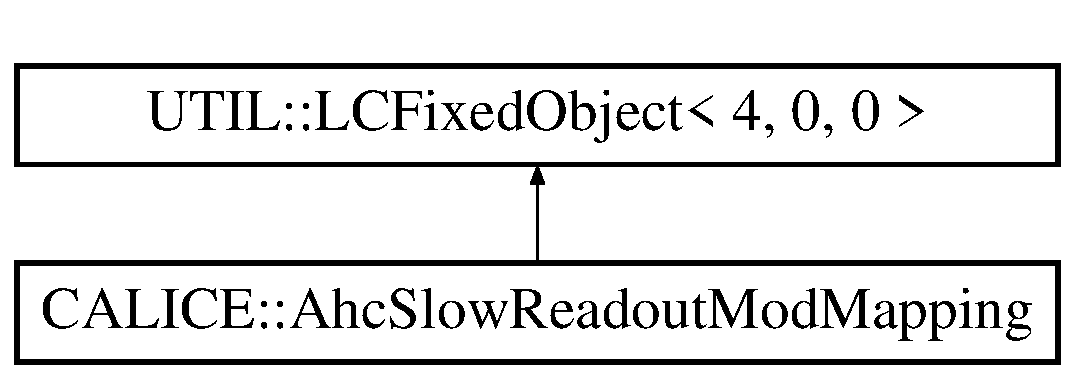
\includegraphics[height=2.000000cm]{classCALICE_1_1AhcSlowReadoutModMapping}
\end{center}
\end{figure}
\subsection*{Public Member Functions}
\begin{DoxyCompactItemize}
\item 
{\bf Ahc\-Slow\-Readout\-Mod\-Mapping} (const int module, const int C\-M\-Brecord\-Label, const int H\-Vrecord\-Label, const int L\-Vrecord\-Label)\label{classCALICE_1_1AhcSlowReadoutModMapping_a04259684c066116f68e2f6e6cf95279d}

\begin{DoxyCompactList}\small\item\em Constructor with initial values. \end{DoxyCompactList}\item 
{\bf Ahc\-Slow\-Readout\-Mod\-Mapping} (E\-V\-E\-N\-T\-::\-L\-C\-Object $\ast$object)\label{classCALICE_1_1AhcSlowReadoutModMapping_a6739023171558d8ef871959a68d8236b}

\begin{DoxyCompactList}\small\item\em Constructor from L\-C\-Object. \end{DoxyCompactList}\item 
{\bf $\sim$\-Ahc\-Slow\-Readout\-Mod\-Mapping} ()\label{classCALICE_1_1AhcSlowReadoutModMapping_a89417dbb3a023ddbb4a931d33b6d4ee7}

\begin{DoxyCompactList}\small\item\em Destructor. \end{DoxyCompactList}\item 
void {\bfseries set\-Module} (int module)\label{classCALICE_1_1AhcSlowReadoutModMapping_a1413edfe61deff586222939ba94bee02}

\item 
void {\bfseries set\-C\-M\-Blabel} (int label)\label{classCALICE_1_1AhcSlowReadoutModMapping_a27b72f9ef8901bde36ebc189e93ba0e1}

\item 
void {\bfseries set\-H\-Vlabel} (int label)\label{classCALICE_1_1AhcSlowReadoutModMapping_af52b00986593fbc5be5cb989d1a1ab33}

\item 
void {\bfseries set\-L\-Vlabel} (int label)\label{classCALICE_1_1AhcSlowReadoutModMapping_a50dde0c78870949667e71ce67532e6e5}

\item 
int {\bf get\-Module} () const \label{classCALICE_1_1AhcSlowReadoutModMapping_a835efcca7195eaedbf03c0b1801f2c9b}

\begin{DoxyCompactList}\small\item\em get the module number for which this record is \end{DoxyCompactList}\item 
int {\bf get\-C\-M\-Blabel} () const 
\begin{DoxyCompactList}\small\item\em get the label of the \doxyref{Ahc\-Slow\-Readout\-Mod\-Block}{p.}{classCALICE_1_1AhcSlowReadoutModBlock} holding the data with source C\-M\-B \end{DoxyCompactList}\item 
int {\bf get\-H\-Vlabel} () const 
\begin{DoxyCompactList}\small\item\em get the label of the \doxyref{Ahc\-Slow\-Readout\-Mod\-Block}{p.}{classCALICE_1_1AhcSlowReadoutModBlock} holding the data with source H\-V supply \end{DoxyCompactList}\item 
int {\bf get\-L\-Vlabel} () const 
\begin{DoxyCompactList}\small\item\em get the label of the \doxyref{Ahc\-Slow\-Readout\-Mod\-Block}{p.}{classCALICE_1_1AhcSlowReadoutModBlock} holding the data with source L\-V monitoring \end{DoxyCompactList}\item 
const std\-::string {\bf get\-Type\-Name} () const \label{classCALICE_1_1AhcSlowReadoutModMapping_aeb86619ed81a290c41fcb00ce96489a9}

\begin{DoxyCompactList}\small\item\em Implementation of L\-C\-Generic\-Object\-::get\-Type\-Name. \end{DoxyCompactList}\item 
const std\-::string {\bf get\-Data\-Description} () const \label{classCALICE_1_1AhcSlowReadoutModMapping_a52b2537a461e778f0b4c5e7e2b38218f}

\begin{DoxyCompactList}\small\item\em Implementation of L\-C\-Generic\-Object\-::get\-Data\-Description. \end{DoxyCompactList}\end{DoxyCompactItemize}


\subsection{Detailed Description}
Class to store the mapping corrections for the \doxyref{Ahc\-Slow\-Readout\-Mod\-Block}{p.}{classCALICE_1_1AhcSlowReadoutModBlock}. 

The slow control assembled the data from different modules into the slow control data submitted to the D\-A\-Q during 2006 and 2007. This bug was only fixed in the beginning of 2008 data taking at F\-N\-A\-L. This class holds the relation between data from the module and under which label it was stored.

As the data comes from three different hardware sources (C\-M\-B, H\-V supply and L\-V) the record holds three numbers for the sources. If the data for one source is lost due to mapping errors, the reading will be -\/1.

\begin{DoxyAuthor}{Author}
{\tt Benjamin.\-Lutz@desy.\-de} 
\end{DoxyAuthor}
\begin{DoxyVersion}{Version}
1.\-0 
\end{DoxyVersion}
\begin{DoxyDate}{Date}
November 2008 
\end{DoxyDate}


Definition at line 29 of file Ahc\-Slow\-Readout\-Mod\-Mapping.\-hh.



\subsection{Member Function Documentation}
\index{C\-A\-L\-I\-C\-E\-::\-Ahc\-Slow\-Readout\-Mod\-Mapping@{C\-A\-L\-I\-C\-E\-::\-Ahc\-Slow\-Readout\-Mod\-Mapping}!get\-C\-M\-Blabel@{get\-C\-M\-Blabel}}
\index{get\-C\-M\-Blabel@{get\-C\-M\-Blabel}!CALICE::AhcSlowReadoutModMapping@{C\-A\-L\-I\-C\-E\-::\-Ahc\-Slow\-Readout\-Mod\-Mapping}}
\subsubsection[{get\-C\-M\-Blabel}]{\setlength{\rightskip}{0pt plus 5cm}int C\-A\-L\-I\-C\-E\-::\-Ahc\-Slow\-Readout\-Mod\-Mapping\-::get\-C\-M\-Blabel (
\begin{DoxyParamCaption}
{}
\end{DoxyParamCaption}
) const}\label{classCALICE_1_1AhcSlowReadoutModMapping_a39c6eca8f76b2b4fbfe7335f8fb79d9b}


get the label of the \doxyref{Ahc\-Slow\-Readout\-Mod\-Block}{p.}{classCALICE_1_1AhcSlowReadoutModBlock} holding the data with source C\-M\-B 

\begin{DoxyRemark}{Remarks}
returns -\/1 when the data was lost due to mapping errors 
\end{DoxyRemark}


Definition at line 23 of file Ahc\-Slow\-Readout\-Mod\-Mapping.\-cc.



Referenced by C\-A\-L\-I\-C\-E\-::\-Ahc\-Slow\-Readout\-Mod\-Mapper\-::update\-Mapping().

\index{C\-A\-L\-I\-C\-E\-::\-Ahc\-Slow\-Readout\-Mod\-Mapping@{C\-A\-L\-I\-C\-E\-::\-Ahc\-Slow\-Readout\-Mod\-Mapping}!get\-H\-Vlabel@{get\-H\-Vlabel}}
\index{get\-H\-Vlabel@{get\-H\-Vlabel}!CALICE::AhcSlowReadoutModMapping@{C\-A\-L\-I\-C\-E\-::\-Ahc\-Slow\-Readout\-Mod\-Mapping}}
\subsubsection[{get\-H\-Vlabel}]{\setlength{\rightskip}{0pt plus 5cm}int C\-A\-L\-I\-C\-E\-::\-Ahc\-Slow\-Readout\-Mod\-Mapping\-::get\-H\-Vlabel (
\begin{DoxyParamCaption}
{}
\end{DoxyParamCaption}
) const}\label{classCALICE_1_1AhcSlowReadoutModMapping_aff49b5b29efaabfb24466c01f1486661}


get the label of the \doxyref{Ahc\-Slow\-Readout\-Mod\-Block}{p.}{classCALICE_1_1AhcSlowReadoutModBlock} holding the data with source H\-V supply 

\begin{DoxyRemark}{Remarks}
returns -\/1 when the data was lost due to mapping errors 
\end{DoxyRemark}


Definition at line 26 of file Ahc\-Slow\-Readout\-Mod\-Mapping.\-cc.



Referenced by C\-A\-L\-I\-C\-E\-::\-Ahc\-Slow\-Readout\-Mod\-Mapper\-::update\-Mapping().

\index{C\-A\-L\-I\-C\-E\-::\-Ahc\-Slow\-Readout\-Mod\-Mapping@{C\-A\-L\-I\-C\-E\-::\-Ahc\-Slow\-Readout\-Mod\-Mapping}!get\-L\-Vlabel@{get\-L\-Vlabel}}
\index{get\-L\-Vlabel@{get\-L\-Vlabel}!CALICE::AhcSlowReadoutModMapping@{C\-A\-L\-I\-C\-E\-::\-Ahc\-Slow\-Readout\-Mod\-Mapping}}
\subsubsection[{get\-L\-Vlabel}]{\setlength{\rightskip}{0pt plus 5cm}int C\-A\-L\-I\-C\-E\-::\-Ahc\-Slow\-Readout\-Mod\-Mapping\-::get\-L\-Vlabel (
\begin{DoxyParamCaption}
{}
\end{DoxyParamCaption}
) const}\label{classCALICE_1_1AhcSlowReadoutModMapping_a68c0787c9d421cb85938ecc4e0ca1b27}


get the label of the \doxyref{Ahc\-Slow\-Readout\-Mod\-Block}{p.}{classCALICE_1_1AhcSlowReadoutModBlock} holding the data with source L\-V monitoring 

\begin{DoxyRemark}{Remarks}
returns -\/1 when the data was lost due to mapping errors 
\end{DoxyRemark}


Definition at line 29 of file Ahc\-Slow\-Readout\-Mod\-Mapping.\-cc.



Referenced by C\-A\-L\-I\-C\-E\-::\-Ahc\-Slow\-Readout\-Mod\-Mapper\-::update\-Mapping().



The documentation for this class was generated from the following files\-:\begin{DoxyCompactItemize}
\item 
Ahc\-Slow\-Readout\-Mod\-Mapping.\-hh\item 
Ahc\-Slow\-Readout\-Mod\-Mapping.\-cc\end{DoxyCompactItemize}

\section{C\-A\-L\-I\-C\-E\-:\-:Ahc\-Temp\-Provider Class Reference}
\label{classCALICE_1_1AhcTempProvider}\index{C\-A\-L\-I\-C\-E\-::\-Ahc\-Temp\-Provider@{C\-A\-L\-I\-C\-E\-::\-Ahc\-Temp\-Provider}}


This is an abstract class defining an interface to access the temperatures in single A\-H\-C\-A\-L cells.  




{\ttfamily \#include $<$Ahc\-Temp\-Provider.\-hh$>$}

Inheritance diagram for C\-A\-L\-I\-C\-E\-:\-:Ahc\-Temp\-Provider\-:\begin{figure}[H]
\begin{center}
\leavevmode
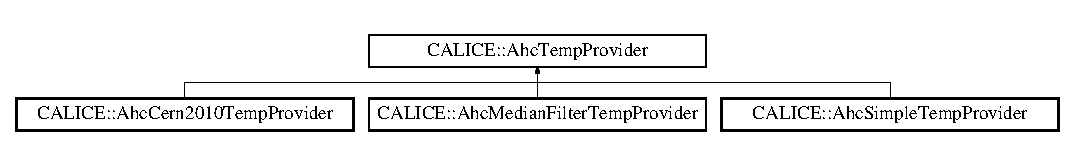
\includegraphics[height=1.530055cm]{classCALICE_1_1AhcTempProvider}
\end{center}
\end{figure}
\subsection*{Public Member Functions}
\begin{DoxyCompactItemize}
\item 
{\bf Ahc\-Temp\-Provider} ()\label{classCALICE_1_1AhcTempProvider_ab4f94c3219c7389ce3871daea4396b4a}

\begin{DoxyCompactList}\small\item\em Default constructor. \end{DoxyCompactList}\item 
virtual {\bf $\sim$\-Ahc\-Temp\-Provider} ()\label{classCALICE_1_1AhcTempProvider_a53d2786bdade2bbcbee773091e774947}

\begin{DoxyCompactList}\small\item\em Default destructor. \end{DoxyCompactList}\item 
virtual float {\bf get\-Cell\-Temp} (int module, int chip, int chan)=0
\begin{DoxyCompactList}\small\item\em Returns the temperature for the cell in the specified module connected to the given chip and channel. \end{DoxyCompactList}\item 
virtual float {\bf get\-Cell\-Temp\-Error} (int module, int chip, int chan)=0
\begin{DoxyCompactList}\small\item\em Returns the error on the temperature for the cell in the specified module connected to the given chip and channel. \end{DoxyCompactList}\item 
virtual void {\bf set\-Ahc\-Sro\-Mod\-Blocks} (lcio\-::\-L\-C\-Collection $\ast$col)\label{classCALICE_1_1AhcTempProvider_a813430a9d33851e62c60b8d6e642fc13}

\begin{DoxyCompactList}\small\item\em Set the collection of \doxyref{Ahc\-Slow\-Readout\-Mod\-Block}{p.}{classCALICE_1_1AhcSlowReadoutModBlock} objects to extract the temperature data from. \end{DoxyCompactList}\item 
virtual float {\bf get\-Avg\-Temp} ()=0\label{classCALICE_1_1AhcTempProvider_a69b50b787f49a84132c7a264516bcf1f}

\begin{DoxyCompactList}\small\item\em Returns the average calorimeter temperature. \end{DoxyCompactList}\item 
virtual float {\bf get\-Avg\-Module\-Temp} (unsigned module)=0\label{classCALICE_1_1AhcTempProvider_a1d4cf73aa7a2308ef910247cc1612760}

\begin{DoxyCompactList}\small\item\em Returns the average module temperature. \end{DoxyCompactList}\item 
virtual float {\bf get\-Sensor\-Temp} (int module, int sensor)=0
\begin{DoxyCompactList}\small\item\em Returns the temperature of the specified sensor in the given module. \end{DoxyCompactList}\item 
virtual void {\bf set\-Calibrations} (lcio\-::\-L\-C\-Collection $\ast$col)\label{classCALICE_1_1AhcTempProvider_a9f7ff35b597b659d1de162dbfd4a34c8}

\begin{DoxyCompactList}\small\item\em Set the collection of \doxyref{Simple\-Value}{p.}{classCALICE_1_1SimpleValue} objects to use for the offset calibrations of the temperature sensors. \end{DoxyCompactList}\item 
virtual void {\bf set\-Sanity\-Range} (float min, float max)
\begin{DoxyCompactList}\small\item\em Define a sanity range of temperature values that make sense. \end{DoxyCompactList}\end{DoxyCompactItemize}
\subsection*{Static Public Attributes}
\begin{DoxyCompactItemize}
\item 
static const unsigned {\bfseries N\-\_\-\-M\-O\-D\-U\-L\-E\-S} = 38\label{classCALICE_1_1AhcTempProvider_a2fb5517d9cf3179ccb581d37cc91097a}

\item 
static const unsigned {\bfseries N\-\_\-\-S\-E\-N\-S\-O\-R\-S} = 5\label{classCALICE_1_1AhcTempProvider_adfe5f33f2eeae2901e32edca4515cd20}

\end{DoxyCompactItemize}
\subsection*{Protected Member Functions}
\begin{DoxyCompactItemize}
\item 
virtual void {\bf update\-Cache} ()
\begin{DoxyCompactList}\small\item\em This function updates the internal 'cache' for the temperature values from the five sensors and applies the calibration offsets, if available. \end{DoxyCompactList}\end{DoxyCompactItemize}
\subsection*{Protected Attributes}
\begin{DoxyCompactItemize}
\item 
bool {\bf new\-Sro\-Mod\-Col}
\begin{DoxyCompactList}\small\item\em If true this indicates that set\-Sro\-Mod\-Blocks() was called and a new collection of Ahc\-Sro\-Mod\-Block objects was set. \end{DoxyCompactList}\item 
bool {\bf new\-Calib\-Col}
\begin{DoxyCompactList}\small\item\em If true this indicates that \doxyref{set\-Calibrations()}{p.}{classCALICE_1_1AhcTempProvider_a9f7ff35b597b659d1de162dbfd4a34c8} was called and a new collection of calibrations was set. \end{DoxyCompactList}\item 
bool {\bf new\-Sanity\-Range}
\begin{DoxyCompactList}\small\item\em If true this indicates that \doxyref{set\-Sanity\-Range()}{p.}{classCALICE_1_1AhcTempProvider_add95eab55a99250ec9f0666fc34ba40d} was called and a new sanity range was set. \end{DoxyCompactList}\item 
std\-::vector$<$ std\-::vector$<$ float $>$ $>$ {\bf sensor\-Temp}
\begin{DoxyCompactList}\small\item\em This is a 'cache' for the values of the temperature sensors after calibration and and correction. \end{DoxyCompactList}\item 
std\-::vector$<$ std\-::vector$<$ float $>$ $>$ {\bf sensor\-Temp\-Error}
\begin{DoxyCompactList}\small\item\em This is a 'cache' for the errors on the values of the temperature sensors after calibration and and correction. \end{DoxyCompactList}\item 
std\-::vector$<$ std\-::vector$<$ float $>$ $>$ {\bf sensor\-Calib}
\begin{DoxyCompactList}\small\item\em This is a 'cache' for the calibration offsets for the temperature sensors. \end{DoxyCompactList}\item 
std\-::vector$<$ std\-::vector$<$ float $>$ $>$ {\bf sensor\-Calib\-Error}
\begin{DoxyCompactList}\small\item\em This is a 'cache' for the errors on the calibration offsets for the temperature sensors. \end{DoxyCompactList}\item 
std\-::vector$<$ std\-::vector$<$ int $>$ $>$ {\bf sensor\-Calib\-Status}\label{classCALICE_1_1AhcTempProvider_af49e3cc723e4ce780660fe181fd2b40f}

\begin{DoxyCompactList}\small\item\em Vector to save the status of the calibration offsets. \end{DoxyCompactList}\item 
float {\bf \-\_\-sanity\-Min}\label{classCALICE_1_1AhcTempProvider_acdf8e26d39ac276e7eac53b2746348c2}

\begin{DoxyCompactList}\small\item\em Lower limit of the sanity range. \end{DoxyCompactList}\item 
float {\bf \-\_\-sanity\-Max}\label{classCALICE_1_1AhcTempProvider_a5c8919447ae0eece8b050ea21bc80e15}

\begin{DoxyCompactList}\small\item\em Upper limit of the sanity range. \end{DoxyCompactList}\item 
lcio\-::\-L\-C\-Collection $\ast$ {\bf \-\_\-sro\-Mod\-Col}\label{classCALICE_1_1AhcTempProvider_a6d03fdcfc0a4fedc590597f4383d36ae}

\begin{DoxyCompactList}\small\item\em A pointer to the L\-C\-Collection containing the Ahc\-Slow\-Read\-Out objects. \end{DoxyCompactList}\item 
lcio\-::\-L\-C\-Collection $\ast$ {\bf \-\_\-calib\-Col}\label{classCALICE_1_1AhcTempProvider_aed886ffef7d22bdcfbfa4e00b6c27f9f}

\begin{DoxyCompactList}\small\item\em A pointer to the L\-C\-Collection containing the calibration offsets objects. \end{DoxyCompactList}\end{DoxyCompactItemize}


\subsection{Detailed Description}
This is an abstract class defining an interface to access the temperatures in single A\-H\-C\-A\-L cells. 

Definition at line 21 of file Ahc\-Temp\-Provider.\-hh.



\subsection{Member Function Documentation}
\index{C\-A\-L\-I\-C\-E\-::\-Ahc\-Temp\-Provider@{C\-A\-L\-I\-C\-E\-::\-Ahc\-Temp\-Provider}!get\-Cell\-Temp@{get\-Cell\-Temp}}
\index{get\-Cell\-Temp@{get\-Cell\-Temp}!CALICE::AhcTempProvider@{C\-A\-L\-I\-C\-E\-::\-Ahc\-Temp\-Provider}}
\subsubsection[{get\-Cell\-Temp}]{\setlength{\rightskip}{0pt plus 5cm}virtual float C\-A\-L\-I\-C\-E\-::\-Ahc\-Temp\-Provider\-::get\-Cell\-Temp (
\begin{DoxyParamCaption}
\item[{int}]{module, }
\item[{int}]{chip, }
\item[{int}]{chan}
\end{DoxyParamCaption}
)\hspace{0.3cm}{\ttfamily [pure virtual]}}\label{classCALICE_1_1AhcTempProvider_aa12c75d45d7ade54316dd113a6bab2d1}


Returns the temperature for the cell in the specified module connected to the given chip and channel. 

This is only the definition of the interface, a concrete funtion has to be implemented in a derived class. Note\-: Modules are counted from 1! The valid range for module numbers thus is 1 to 38. 

Implemented in {\bf C\-A\-L\-I\-C\-E\-::\-Ahc\-Median\-Filter\-Temp\-Provider} \doxyref{}{p.}{classCALICE_1_1AhcMedianFilterTempProvider_a2d5865711d94a975e593df2713608880}, {\bf C\-A\-L\-I\-C\-E\-::\-Ahc\-Simple\-Temp\-Provider} \doxyref{}{p.}{classCALICE_1_1AhcSimpleTempProvider_aff9186dfdab4801e41540f1d63428e3f}, and {\bf C\-A\-L\-I\-C\-E\-::\-Ahc\-Cern2010\-Temp\-Provider} \doxyref{}{p.}{classCALICE_1_1AhcCern2010TempProvider_a50c27d4ce36e8bda65a50c41f3f55835}.

\index{C\-A\-L\-I\-C\-E\-::\-Ahc\-Temp\-Provider@{C\-A\-L\-I\-C\-E\-::\-Ahc\-Temp\-Provider}!get\-Cell\-Temp\-Error@{get\-Cell\-Temp\-Error}}
\index{get\-Cell\-Temp\-Error@{get\-Cell\-Temp\-Error}!CALICE::AhcTempProvider@{C\-A\-L\-I\-C\-E\-::\-Ahc\-Temp\-Provider}}
\subsubsection[{get\-Cell\-Temp\-Error}]{\setlength{\rightskip}{0pt plus 5cm}virtual float C\-A\-L\-I\-C\-E\-::\-Ahc\-Temp\-Provider\-::get\-Cell\-Temp\-Error (
\begin{DoxyParamCaption}
\item[{int}]{module, }
\item[{int}]{chip, }
\item[{int}]{chan}
\end{DoxyParamCaption}
)\hspace{0.3cm}{\ttfamily [pure virtual]}}\label{classCALICE_1_1AhcTempProvider_a72d155c16a772198a0587886e8d56102}


Returns the error on the temperature for the cell in the specified module connected to the given chip and channel. 

This is only the definition of the interface, a concrete funtion has to be implemented in a derived class. Note\-: Modules are counted from 1! The valid range for module numbers thus is 1 to 38. 

Implemented in {\bf C\-A\-L\-I\-C\-E\-::\-Ahc\-Median\-Filter\-Temp\-Provider} \doxyref{}{p.}{classCALICE_1_1AhcMedianFilterTempProvider_ace083f026078087a40383dd051d34843}, {\bf C\-A\-L\-I\-C\-E\-::\-Ahc\-Simple\-Temp\-Provider} \doxyref{}{p.}{classCALICE_1_1AhcSimpleTempProvider_a2d3cd7fd1a3f144f62991e39b44d016f}, and {\bf C\-A\-L\-I\-C\-E\-::\-Ahc\-Cern2010\-Temp\-Provider} \doxyref{}{p.}{classCALICE_1_1AhcCern2010TempProvider_a49df2cbe0a0e947fc69fc2f9e6d4af7e}.

\index{C\-A\-L\-I\-C\-E\-::\-Ahc\-Temp\-Provider@{C\-A\-L\-I\-C\-E\-::\-Ahc\-Temp\-Provider}!get\-Sensor\-Temp@{get\-Sensor\-Temp}}
\index{get\-Sensor\-Temp@{get\-Sensor\-Temp}!CALICE::AhcTempProvider@{C\-A\-L\-I\-C\-E\-::\-Ahc\-Temp\-Provider}}
\subsubsection[{get\-Sensor\-Temp}]{\setlength{\rightskip}{0pt plus 5cm}virtual float C\-A\-L\-I\-C\-E\-::\-Ahc\-Temp\-Provider\-::get\-Sensor\-Temp (
\begin{DoxyParamCaption}
\item[{int}]{module, }
\item[{int}]{sensor}
\end{DoxyParamCaption}
)\hspace{0.3cm}{\ttfamily [pure virtual]}}\label{classCALICE_1_1AhcTempProvider_a9db9d635f879ed75ae983bbeca800ff8}


Returns the temperature of the specified sensor in the given module. 



Implemented in {\bf C\-A\-L\-I\-C\-E\-::\-Ahc\-Median\-Filter\-Temp\-Provider} \doxyref{}{p.}{classCALICE_1_1AhcMedianFilterTempProvider_ac9f730849a87bda3106773b7dc869f2e}, {\bf C\-A\-L\-I\-C\-E\-::\-Ahc\-Simple\-Temp\-Provider} \doxyref{}{p.}{classCALICE_1_1AhcSimpleTempProvider_ab61d13863930498a336476d9ac049b2e}, and {\bf C\-A\-L\-I\-C\-E\-::\-Ahc\-Cern2010\-Temp\-Provider} \doxyref{}{p.}{classCALICE_1_1AhcCern2010TempProvider_ab8220e0d64d2785cc896beae3db00e12}.

\index{C\-A\-L\-I\-C\-E\-::\-Ahc\-Temp\-Provider@{C\-A\-L\-I\-C\-E\-::\-Ahc\-Temp\-Provider}!set\-Sanity\-Range@{set\-Sanity\-Range}}
\index{set\-Sanity\-Range@{set\-Sanity\-Range}!CALICE::AhcTempProvider@{C\-A\-L\-I\-C\-E\-::\-Ahc\-Temp\-Provider}}
\subsubsection[{set\-Sanity\-Range}]{\setlength{\rightskip}{0pt plus 5cm}void C\-A\-L\-I\-C\-E\-::\-Ahc\-Temp\-Provider\-::set\-Sanity\-Range (
\begin{DoxyParamCaption}
\item[{float}]{min, }
\item[{float}]{max}
\end{DoxyParamCaption}
)\hspace{0.3cm}{\ttfamily [virtual]}}\label{classCALICE_1_1AhcTempProvider_add95eab55a99250ec9f0666fc34ba40d}


Define a sanity range of temperature values that make sense. 

There are some dead sensors, e.\-g giving only the value 117 degree Celsius, which makes no sense. Also a temperature of zero degree Celsius is very unlikely. With this function you specify the range in which temperatures are accepted. A sensible range would be 10 to 50 degree Celsius for example. Note\-: This is an abstract class -\/ how data from temperature sensors giving values outside this range is handled is only depended from the implementation of in the derived class. It may completely ignore the range specified here. 

Definition at line 52 of file Ahc\-Temp\-Provider.\-cc.



References \-\_\-sanity\-Max, \-\_\-sanity\-Min, and new\-Sanity\-Range.

\index{C\-A\-L\-I\-C\-E\-::\-Ahc\-Temp\-Provider@{C\-A\-L\-I\-C\-E\-::\-Ahc\-Temp\-Provider}!update\-Cache@{update\-Cache}}
\index{update\-Cache@{update\-Cache}!CALICE::AhcTempProvider@{C\-A\-L\-I\-C\-E\-::\-Ahc\-Temp\-Provider}}
\subsubsection[{update\-Cache}]{\setlength{\rightskip}{0pt plus 5cm}void C\-A\-L\-I\-C\-E\-::\-Ahc\-Temp\-Provider\-::update\-Cache (
\begin{DoxyParamCaption}
{}
\end{DoxyParamCaption}
)\hspace{0.3cm}{\ttfamily [protected]}, {\ttfamily [virtual]}}\label{classCALICE_1_1AhcTempProvider_aaf2e7780e46882ba4fe8755c8bad2237}


This function updates the internal 'cache' for the temperature values from the five sensors and applies the calibration offsets, if available. 

It should be called everytime a new collection of temperatures or calibrations have been at set or the sanity range has been changed, i.\-e. if one of new\-Sro\-Mod\-Col, new\-Calib\-Col or new\-Sanity\-Range is true. 

Definition at line 59 of file Ahc\-Temp\-Provider.\-cc.



References \-\_\-calib\-Col, \-\_\-sro\-Mod\-Col, C\-A\-L\-I\-C\-E\-::\-Scint\-Calo\-Slow\-Readout\-Mod\-Block\-::get\-Module\-Number(), new\-Calib\-Col, new\-Sro\-Mod\-Col, sensor\-Calib, and sensor\-Temp.



Referenced by C\-A\-L\-I\-C\-E\-::\-Ahc\-Simple\-Temp\-Provider\-::apply\-Correction(), and C\-A\-L\-I\-C\-E\-::\-Ahc\-Median\-Filter\-Temp\-Provider\-::apply\-Correction().



\subsection{Field Documentation}
\index{C\-A\-L\-I\-C\-E\-::\-Ahc\-Temp\-Provider@{C\-A\-L\-I\-C\-E\-::\-Ahc\-Temp\-Provider}!new\-Calib\-Col@{new\-Calib\-Col}}
\index{new\-Calib\-Col@{new\-Calib\-Col}!CALICE::AhcTempProvider@{C\-A\-L\-I\-C\-E\-::\-Ahc\-Temp\-Provider}}
\subsubsection[{new\-Calib\-Col}]{\setlength{\rightskip}{0pt plus 5cm}bool C\-A\-L\-I\-C\-E\-::\-Ahc\-Temp\-Provider\-::new\-Calib\-Col\hspace{0.3cm}{\ttfamily [protected]}}\label{classCALICE_1_1AhcTempProvider_a5d97a51401f30bf5afed91749503a2f5}


If true this indicates that \doxyref{set\-Calibrations()}{p.}{classCALICE_1_1AhcTempProvider_a9f7ff35b597b659d1de162dbfd4a34c8} was called and a new collection of calibrations was set. 

Can be useful for caching to achieve speedup in processing. 

Definition at line 116 of file Ahc\-Temp\-Provider.\-hh.



Referenced by C\-A\-L\-I\-C\-E\-::\-Ahc\-Simple\-Temp\-Provider\-::apply\-Correction(), C\-A\-L\-I\-C\-E\-::\-Ahc\-Median\-Filter\-Temp\-Provider\-::apply\-Correction(), C\-A\-L\-I\-C\-E\-::\-Ahc\-Cern2010\-Temp\-Provider\-::get\-Avg\-Module\-Temp(), C\-A\-L\-I\-C\-E\-::\-Ahc\-Simple\-Temp\-Provider\-::get\-Avg\-Module\-Temp(), C\-A\-L\-I\-C\-E\-::\-Ahc\-Median\-Filter\-Temp\-Provider\-::get\-Avg\-Module\-Temp(), C\-A\-L\-I\-C\-E\-::\-Ahc\-Cern2010\-Temp\-Provider\-::get\-Avg\-Temp(), C\-A\-L\-I\-C\-E\-::\-Ahc\-Simple\-Temp\-Provider\-::get\-Avg\-Temp(), C\-A\-L\-I\-C\-E\-::\-Ahc\-Median\-Filter\-Temp\-Provider\-::get\-Avg\-Temp(), C\-A\-L\-I\-C\-E\-::\-Ahc\-Cern2010\-Temp\-Provider\-::get\-Cell\-Temp(), C\-A\-L\-I\-C\-E\-::\-Ahc\-Simple\-Temp\-Provider\-::get\-Cell\-Temp(), C\-A\-L\-I\-C\-E\-::\-Ahc\-Median\-Filter\-Temp\-Provider\-::get\-Cell\-Temp(), C\-A\-L\-I\-C\-E\-::\-Ahc\-Cern2010\-Temp\-Provider\-::get\-Cell\-Temp\-Error(), C\-A\-L\-I\-C\-E\-::\-Ahc\-Simple\-Temp\-Provider\-::get\-Cell\-Temp\-Error(), C\-A\-L\-I\-C\-E\-::\-Ahc\-Median\-Filter\-Temp\-Provider\-::get\-Cell\-Temp\-Error(), C\-A\-L\-I\-C\-E\-::\-Ahc\-Cern2010\-Temp\-Provider\-::get\-Sensor\-Temp(), C\-A\-L\-I\-C\-E\-::\-Ahc\-Simple\-Temp\-Provider\-::get\-Sensor\-Temp(), C\-A\-L\-I\-C\-E\-::\-Ahc\-Median\-Filter\-Temp\-Provider\-::get\-Sensor\-Temp(), set\-Calibrations(), and update\-Cache().

\index{C\-A\-L\-I\-C\-E\-::\-Ahc\-Temp\-Provider@{C\-A\-L\-I\-C\-E\-::\-Ahc\-Temp\-Provider}!new\-Sanity\-Range@{new\-Sanity\-Range}}
\index{new\-Sanity\-Range@{new\-Sanity\-Range}!CALICE::AhcTempProvider@{C\-A\-L\-I\-C\-E\-::\-Ahc\-Temp\-Provider}}
\subsubsection[{new\-Sanity\-Range}]{\setlength{\rightskip}{0pt plus 5cm}bool C\-A\-L\-I\-C\-E\-::\-Ahc\-Temp\-Provider\-::new\-Sanity\-Range\hspace{0.3cm}{\ttfamily [protected]}}\label{classCALICE_1_1AhcTempProvider_afc923ba1a81304d4165060e6cb8bfe87}


If true this indicates that \doxyref{set\-Sanity\-Range()}{p.}{classCALICE_1_1AhcTempProvider_add95eab55a99250ec9f0666fc34ba40d} was called and a new sanity range was set. 

Can be useful for caching to achieve speedup in processing. 

Definition at line 123 of file Ahc\-Temp\-Provider.\-hh.



Referenced by C\-A\-L\-I\-C\-E\-::\-Ahc\-Simple\-Temp\-Provider\-::apply\-Correction(), C\-A\-L\-I\-C\-E\-::\-Ahc\-Median\-Filter\-Temp\-Provider\-::apply\-Correction(), C\-A\-L\-I\-C\-E\-::\-Ahc\-Cern2010\-Temp\-Provider\-::get\-Avg\-Module\-Temp(), C\-A\-L\-I\-C\-E\-::\-Ahc\-Simple\-Temp\-Provider\-::get\-Avg\-Module\-Temp(), C\-A\-L\-I\-C\-E\-::\-Ahc\-Median\-Filter\-Temp\-Provider\-::get\-Avg\-Module\-Temp(), C\-A\-L\-I\-C\-E\-::\-Ahc\-Cern2010\-Temp\-Provider\-::get\-Avg\-Temp(), C\-A\-L\-I\-C\-E\-::\-Ahc\-Simple\-Temp\-Provider\-::get\-Avg\-Temp(), C\-A\-L\-I\-C\-E\-::\-Ahc\-Median\-Filter\-Temp\-Provider\-::get\-Avg\-Temp(), C\-A\-L\-I\-C\-E\-::\-Ahc\-Cern2010\-Temp\-Provider\-::get\-Cell\-Temp(), C\-A\-L\-I\-C\-E\-::\-Ahc\-Simple\-Temp\-Provider\-::get\-Cell\-Temp(), C\-A\-L\-I\-C\-E\-::\-Ahc\-Median\-Filter\-Temp\-Provider\-::get\-Cell\-Temp(), C\-A\-L\-I\-C\-E\-::\-Ahc\-Cern2010\-Temp\-Provider\-::get\-Cell\-Temp\-Error(), C\-A\-L\-I\-C\-E\-::\-Ahc\-Simple\-Temp\-Provider\-::get\-Cell\-Temp\-Error(), C\-A\-L\-I\-C\-E\-::\-Ahc\-Median\-Filter\-Temp\-Provider\-::get\-Cell\-Temp\-Error(), C\-A\-L\-I\-C\-E\-::\-Ahc\-Cern2010\-Temp\-Provider\-::get\-Sensor\-Temp(), C\-A\-L\-I\-C\-E\-::\-Ahc\-Simple\-Temp\-Provider\-::get\-Sensor\-Temp(), C\-A\-L\-I\-C\-E\-::\-Ahc\-Median\-Filter\-Temp\-Provider\-::get\-Sensor\-Temp(), and set\-Sanity\-Range().

\index{C\-A\-L\-I\-C\-E\-::\-Ahc\-Temp\-Provider@{C\-A\-L\-I\-C\-E\-::\-Ahc\-Temp\-Provider}!new\-Sro\-Mod\-Col@{new\-Sro\-Mod\-Col}}
\index{new\-Sro\-Mod\-Col@{new\-Sro\-Mod\-Col}!CALICE::AhcTempProvider@{C\-A\-L\-I\-C\-E\-::\-Ahc\-Temp\-Provider}}
\subsubsection[{new\-Sro\-Mod\-Col}]{\setlength{\rightskip}{0pt plus 5cm}bool C\-A\-L\-I\-C\-E\-::\-Ahc\-Temp\-Provider\-::new\-Sro\-Mod\-Col\hspace{0.3cm}{\ttfamily [protected]}}\label{classCALICE_1_1AhcTempProvider_a74d1c14bbe08ef50cacf1b52c2731904}


If true this indicates that set\-Sro\-Mod\-Blocks() was called and a new collection of Ahc\-Sro\-Mod\-Block objects was set. 

Can be useful for caching to achieve speedup in processing. 

Definition at line 109 of file Ahc\-Temp\-Provider.\-hh.



Referenced by C\-A\-L\-I\-C\-E\-::\-Ahc\-Simple\-Temp\-Provider\-::apply\-Correction(), C\-A\-L\-I\-C\-E\-::\-Ahc\-Median\-Filter\-Temp\-Provider\-::apply\-Correction(), C\-A\-L\-I\-C\-E\-::\-Ahc\-Cern2010\-Temp\-Provider\-::get\-Avg\-Module\-Temp(), C\-A\-L\-I\-C\-E\-::\-Ahc\-Simple\-Temp\-Provider\-::get\-Avg\-Module\-Temp(), C\-A\-L\-I\-C\-E\-::\-Ahc\-Median\-Filter\-Temp\-Provider\-::get\-Avg\-Module\-Temp(), C\-A\-L\-I\-C\-E\-::\-Ahc\-Cern2010\-Temp\-Provider\-::get\-Avg\-Temp(), C\-A\-L\-I\-C\-E\-::\-Ahc\-Simple\-Temp\-Provider\-::get\-Avg\-Temp(), C\-A\-L\-I\-C\-E\-::\-Ahc\-Median\-Filter\-Temp\-Provider\-::get\-Avg\-Temp(), C\-A\-L\-I\-C\-E\-::\-Ahc\-Cern2010\-Temp\-Provider\-::get\-Cell\-Temp(), C\-A\-L\-I\-C\-E\-::\-Ahc\-Simple\-Temp\-Provider\-::get\-Cell\-Temp(), C\-A\-L\-I\-C\-E\-::\-Ahc\-Median\-Filter\-Temp\-Provider\-::get\-Cell\-Temp(), C\-A\-L\-I\-C\-E\-::\-Ahc\-Cern2010\-Temp\-Provider\-::get\-Cell\-Temp\-Error(), C\-A\-L\-I\-C\-E\-::\-Ahc\-Simple\-Temp\-Provider\-::get\-Cell\-Temp\-Error(), C\-A\-L\-I\-C\-E\-::\-Ahc\-Median\-Filter\-Temp\-Provider\-::get\-Cell\-Temp\-Error(), C\-A\-L\-I\-C\-E\-::\-Ahc\-Cern2010\-Temp\-Provider\-::get\-Sensor\-Temp(), C\-A\-L\-I\-C\-E\-::\-Ahc\-Simple\-Temp\-Provider\-::get\-Sensor\-Temp(), C\-A\-L\-I\-C\-E\-::\-Ahc\-Median\-Filter\-Temp\-Provider\-::get\-Sensor\-Temp(), set\-Ahc\-Sro\-Mod\-Blocks(), and update\-Cache().

\index{C\-A\-L\-I\-C\-E\-::\-Ahc\-Temp\-Provider@{C\-A\-L\-I\-C\-E\-::\-Ahc\-Temp\-Provider}!sensor\-Calib@{sensor\-Calib}}
\index{sensor\-Calib@{sensor\-Calib}!CALICE::AhcTempProvider@{C\-A\-L\-I\-C\-E\-::\-Ahc\-Temp\-Provider}}
\subsubsection[{sensor\-Calib}]{\setlength{\rightskip}{0pt plus 5cm}std\-::vector$<$ std\-::vector$<$ float $>$ $>$ C\-A\-L\-I\-C\-E\-::\-Ahc\-Temp\-Provider\-::sensor\-Calib\hspace{0.3cm}{\ttfamily [protected]}}\label{classCALICE_1_1AhcTempProvider_ad4116a88a804429437ab8c940d555eba}


This is a 'cache' for the calibration offsets for the temperature sensors. 

It is a vector of a vector, first key is module (0...37) and second key is sensor number (0...4). It is filled when \doxyref{set\-Calibrations()}{p.}{classCALICE_1_1AhcTempProvider_a9f7ff35b597b659d1de162dbfd4a34c8} is called; 

Definition at line 149 of file Ahc\-Temp\-Provider.\-hh.



Referenced by Ahc\-Temp\-Provider(), set\-Calibrations(), and update\-Cache().

\index{C\-A\-L\-I\-C\-E\-::\-Ahc\-Temp\-Provider@{C\-A\-L\-I\-C\-E\-::\-Ahc\-Temp\-Provider}!sensor\-Calib\-Error@{sensor\-Calib\-Error}}
\index{sensor\-Calib\-Error@{sensor\-Calib\-Error}!CALICE::AhcTempProvider@{C\-A\-L\-I\-C\-E\-::\-Ahc\-Temp\-Provider}}
\subsubsection[{sensor\-Calib\-Error}]{\setlength{\rightskip}{0pt plus 5cm}std\-::vector$<$ std\-::vector$<$ float $>$ $>$ C\-A\-L\-I\-C\-E\-::\-Ahc\-Temp\-Provider\-::sensor\-Calib\-Error\hspace{0.3cm}{\ttfamily [protected]}}\label{classCALICE_1_1AhcTempProvider_a9a8b275ae8bf46f0ac30504ce2b437b0}


This is a 'cache' for the errors on the calibration offsets for the temperature sensors. 

It is a vector of a vector, first key is module (0...37) and second key is sensor number (0...4). It is filled when \doxyref{set\-Calibrations()}{p.}{classCALICE_1_1AhcTempProvider_a9f7ff35b597b659d1de162dbfd4a34c8} is called; 

Definition at line 156 of file Ahc\-Temp\-Provider.\-hh.



Referenced by Ahc\-Temp\-Provider(), and set\-Calibrations().

\index{C\-A\-L\-I\-C\-E\-::\-Ahc\-Temp\-Provider@{C\-A\-L\-I\-C\-E\-::\-Ahc\-Temp\-Provider}!sensor\-Temp@{sensor\-Temp}}
\index{sensor\-Temp@{sensor\-Temp}!CALICE::AhcTempProvider@{C\-A\-L\-I\-C\-E\-::\-Ahc\-Temp\-Provider}}
\subsubsection[{sensor\-Temp}]{\setlength{\rightskip}{0pt plus 5cm}std\-::vector$<$ std\-::vector$<$ float $>$ $>$ C\-A\-L\-I\-C\-E\-::\-Ahc\-Temp\-Provider\-::sensor\-Temp\hspace{0.3cm}{\ttfamily [protected]}}\label{classCALICE_1_1AhcTempProvider_a4e5a07c38f63a12bc38eebff556ac750}


This is a 'cache' for the values of the temperature sensors after calibration and and correction. 

It is a vector of a vector, first key is module (0...37) and second key is sensor number (0...4). Note\-: this is only an abstract class, look at \doxyref{get\-Cell\-Temp()}{p.}{classCALICE_1_1AhcTempProvider_aa12c75d45d7ade54316dd113a6bab2d1} and apply\-Calib\-Corr() in your implentation to understand how and when it is updated. 

Definition at line 132 of file Ahc\-Temp\-Provider.\-hh.



Referenced by Ahc\-Temp\-Provider(), C\-A\-L\-I\-C\-E\-::\-Ahc\-Simple\-Temp\-Provider\-::apply\-Correction(), C\-A\-L\-I\-C\-E\-::\-Ahc\-Median\-Filter\-Temp\-Provider\-::apply\-Correction(), C\-A\-L\-I\-C\-E\-::\-Ahc\-Cern2010\-Temp\-Provider\-::get\-Cell\-Temp(), C\-A\-L\-I\-C\-E\-::\-Ahc\-Simple\-Temp\-Provider\-::get\-Cell\-Temp(), C\-A\-L\-I\-C\-E\-::\-Ahc\-Median\-Filter\-Temp\-Provider\-::get\-Cell\-Temp(), C\-A\-L\-I\-C\-E\-::\-Ahc\-Cern2010\-Temp\-Provider\-::get\-Sensor\-Temp(), C\-A\-L\-I\-C\-E\-::\-Ahc\-Simple\-Temp\-Provider\-::get\-Sensor\-Temp(), C\-A\-L\-I\-C\-E\-::\-Ahc\-Median\-Filter\-Temp\-Provider\-::get\-Sensor\-Temp(), and update\-Cache().

\index{C\-A\-L\-I\-C\-E\-::\-Ahc\-Temp\-Provider@{C\-A\-L\-I\-C\-E\-::\-Ahc\-Temp\-Provider}!sensor\-Temp\-Error@{sensor\-Temp\-Error}}
\index{sensor\-Temp\-Error@{sensor\-Temp\-Error}!CALICE::AhcTempProvider@{C\-A\-L\-I\-C\-E\-::\-Ahc\-Temp\-Provider}}
\subsubsection[{sensor\-Temp\-Error}]{\setlength{\rightskip}{0pt plus 5cm}std\-::vector$<$ std\-::vector$<$ float $>$ $>$ C\-A\-L\-I\-C\-E\-::\-Ahc\-Temp\-Provider\-::sensor\-Temp\-Error\hspace{0.3cm}{\ttfamily [protected]}}\label{classCALICE_1_1AhcTempProvider_acf152646f43cf38d95af642369fc7b71}


This is a 'cache' for the errors on the values of the temperature sensors after calibration and and correction. 

It is a vector of a vector, first key is module (0...37) and second key is sensor number (0...4). Note\-: this is only an abstract class, look at \doxyref{get\-Cell\-Temp\-Error()}{p.}{classCALICE_1_1AhcTempProvider_a72d155c16a772198a0587886e8d56102} and apply\-Calib\-Corr() in your implentation to understand how and when it is updated. 

Definition at line 142 of file Ahc\-Temp\-Provider.\-hh.



Referenced by Ahc\-Temp\-Provider(), C\-A\-L\-I\-C\-E\-::\-Ahc\-Simple\-Temp\-Provider\-::apply\-Correction(), C\-A\-L\-I\-C\-E\-::\-Ahc\-Median\-Filter\-Temp\-Provider\-::apply\-Correction(), C\-A\-L\-I\-C\-E\-::\-Ahc\-Cern2010\-Temp\-Provider\-::get\-Cell\-Temp\-Error(), C\-A\-L\-I\-C\-E\-::\-Ahc\-Simple\-Temp\-Provider\-::get\-Cell\-Temp\-Error(), and C\-A\-L\-I\-C\-E\-::\-Ahc\-Median\-Filter\-Temp\-Provider\-::get\-Cell\-Temp\-Error().



The documentation for this class was generated from the following files\-:\begin{DoxyCompactItemize}
\item 
Ahc\-Temp\-Provider.\-hh\item 
Ahc\-Temp\-Provider.\-cc\end{DoxyCompactItemize}

\section{C\-A\-L\-I\-C\-E\-:\-:Ahc\-Temp\-Sensor\-Index Class Reference}
\label{classCALICE_1_1AhcTempSensorIndex}\index{C\-A\-L\-I\-C\-E\-::\-Ahc\-Temp\-Sensor\-Index@{C\-A\-L\-I\-C\-E\-::\-Ahc\-Temp\-Sensor\-Index}}


\doxyref{Ahc\-Temp\-Sensor\-Index}{p.}{classCALICE_1_1AhcTempSensorIndex} represents and Ahcal Temperature Sensor Index So what? it encodes (modules,sensor) into an integer.  




{\ttfamily \#include $<$Ahc\-Temp\-Sensor\-Index.\-hh$>$}

\subsection*{Public Member Functions}
\begin{DoxyCompactItemize}
\item 
{\bfseries Ahc\-Temp\-Sensor\-Index} (int key)\label{classCALICE_1_1AhcTempSensorIndex_aabd05c4d6a8f8c147836f03c17b1972c}

\item 
{\bfseries Ahc\-Temp\-Sensor\-Index} (int module, int sensor)\label{classCALICE_1_1AhcTempSensorIndex_adba3f8bc6b3c7b8cc3d03483bd59efac}

\item 
void {\bfseries set\-Key} (int key)\label{classCALICE_1_1AhcTempSensorIndex_a128b797a06ff96fe81ecbe0eea39c45f}

\item 
void {\bfseries set\-Module} (int m)\label{classCALICE_1_1AhcTempSensorIndex_a7aff7a3110f6b8480aa43dd5579922ad}

\item 
void {\bfseries set\-Sensor} (int s)\label{classCALICE_1_1AhcTempSensorIndex_ae385a5b959af9c6becc0511a6e992fc4}

\item 
int {\bfseries get\-Key} ()\label{classCALICE_1_1AhcTempSensorIndex_aa23bfc8a2b16a1da1a3477f6a00e8dc3}

\item 
int {\bfseries get\-Module} ()\label{classCALICE_1_1AhcTempSensorIndex_a0a7a1fb86bbeaa456b13b135d537dafa}

\item 
int {\bfseries get\-Sensor} ()\label{classCALICE_1_1AhcTempSensorIndex_a0c14a4130dcb7c7d151da0cb3a1082e8}

\end{DoxyCompactItemize}
\subsection*{Static Public Attributes}
\begin{DoxyCompactItemize}
\item 
static const int {\bfseries M\-O\-D\-U\-L\-E\-\_\-\-M\-A\-S\-K} = 0xff00\label{classCALICE_1_1AhcTempSensorIndex_a104e7d97e5ad4b2c0085b7b44c3bff05}

\item 
static const int {\bfseries M\-O\-D\-U\-L\-E\-\_\-\-S\-H\-I\-F\-T} = 8\label{classCALICE_1_1AhcTempSensorIndex_a1e298eabdfb2c9420fb2d4ab5f1f1c51}

\item 
static const int {\bfseries S\-E\-N\-S\-O\-R\-\_\-\-M\-A\-S\-K} = 0xff\label{classCALICE_1_1AhcTempSensorIndex_a848692647cc767fee6915ad6e23933de}

\item 
static const int {\bfseries S\-E\-N\-S\-O\-R\-\_\-\-S\-H\-I\-F\-T} = 0\label{classCALICE_1_1AhcTempSensorIndex_a7286ad523152d148b5578466b8b75767}

\end{DoxyCompactItemize}
\subsection*{Private Attributes}
\begin{DoxyCompactItemize}
\item 
int {\bfseries \-\_\-key}\label{classCALICE_1_1AhcTempSensorIndex_a0f08c7f83deccb6df75cb6e159a446cb}

\end{DoxyCompactItemize}


\subsection{Detailed Description}
\doxyref{Ahc\-Temp\-Sensor\-Index}{p.}{classCALICE_1_1AhcTempSensorIndex} represents and Ahcal Temperature Sensor Index So what? it encodes (modules,sensor) into an integer. 

Definition at line 11 of file Ahc\-Temp\-Sensor\-Index.\-hh.



The documentation for this class was generated from the following files\-:\begin{DoxyCompactItemize}
\item 
Ahc\-Temp\-Sensor\-Index.\-hh\item 
Ahc\-Temp\-Sensor\-Index.\-cc\end{DoxyCompactItemize}

\section{C\-A\-L\-I\-C\-E\-:\-:Ahc\-Vfe\-Configuration\-Block Class Reference}
\label{classCALICE_1_1AhcVfeConfigurationBlock}\index{C\-A\-L\-I\-C\-E\-::\-Ahc\-Vfe\-Configuration\-Block@{C\-A\-L\-I\-C\-E\-::\-Ahc\-Vfe\-Configuration\-Block}}


Interface Class to access the Ahc\-Vfe\-Configuration\-Data.  




{\ttfamily \#include $<$Ahc\-Vfe\-Configuration\-Block.\-hh$>$}

Inheritance diagram for C\-A\-L\-I\-C\-E\-:\-:Ahc\-Vfe\-Configuration\-Block\-:\begin{figure}[H]
\begin{center}
\leavevmode
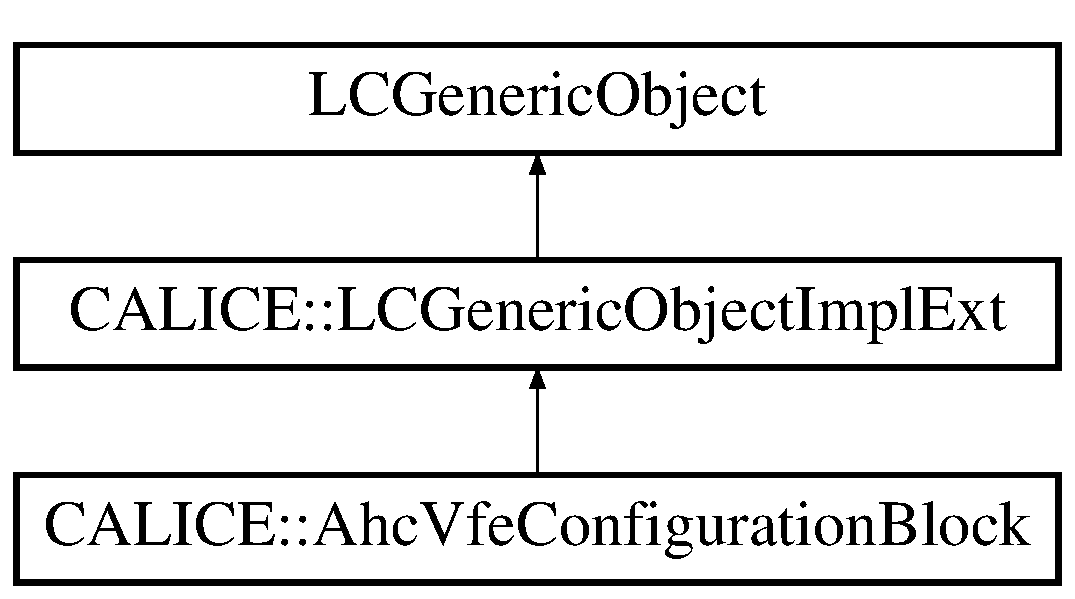
\includegraphics[height=3.000000cm]{classCALICE_1_1AhcVfeConfigurationBlock}
\end{center}
\end{figure}
\subsection*{Public Member Functions}
\begin{DoxyCompactItemize}
\item 
{\bf Ahc\-Vfe\-Configuration\-Block} (int board\-I\-D)
\begin{DoxyCompactList}\small\item\em Convenient c'tor. \end{DoxyCompactList}\item 
{\bf Ahc\-Vfe\-Configuration\-Block} \& {\bf set\-Crate\-I\-D} (short crate\-I\-D)\label{classCALICE_1_1AhcVfeConfigurationBlock_a201e36bf403cffb9903f1566be72818e}

\begin{DoxyCompactList}\small\item\em Set the crate\-I\-D. \end{DoxyCompactList}\item 
short {\bf get\-Crate\-I\-D} () const \label{classCALICE_1_1AhcVfeConfigurationBlock_a19695e1a48f9901745283f645c813a59}

\begin{DoxyCompactList}\small\item\em Get the crate I\-D. \end{DoxyCompactList}\item 
{\bf Ahc\-Vfe\-Configuration\-Block} \& {\bf set\-Slot\-I\-D} (short slot\-I\-D)\label{classCALICE_1_1AhcVfeConfigurationBlock_a6ef47b059a3b1d255c99df87c30782d2}

\begin{DoxyCompactList}\small\item\em Set the Slot I\-D. \end{DoxyCompactList}\item 
short {\bf get\-Slot\-I\-D} () const \label{classCALICE_1_1AhcVfeConfigurationBlock_adba054e559e65594f1477cd578a4230e}

\begin{DoxyCompactList}\small\item\em Get the Slot I\-D. \end{DoxyCompactList}\item 
{\bf Ahc\-Vfe\-Configuration\-Block} \& {\bf set\-Board\-Component\-Number} (short component\-Number)\label{classCALICE_1_1AhcVfeConfigurationBlock_a30f5dff217b1fa44326c86902c1b88ee}

\begin{DoxyCompactList}\small\item\em Set the Board\-Component\-Number. \end{DoxyCompactList}\item 
short {\bf get\-Board\-Component\-Number} () const \label{classCALICE_1_1AhcVfeConfigurationBlock_a434b41151c72986819bf924ae024345c}

\begin{DoxyCompactList}\small\item\em Get the Board\-Component\-Number. \end{DoxyCompactList}\item 
void {\bf set\-Record\-Label} (int label)\label{classCALICE_1_1AhcVfeConfigurationBlock_ab74486109cf73a0bae48ef7a222a73cb}

\begin{DoxyCompactList}\small\item\em Set the Record Label. \end{DoxyCompactList}\item 
short {\bf get\-Record\-Label} () const \label{classCALICE_1_1AhcVfeConfigurationBlock_a95166f80fa388544cefd9bff2bcdf83c}

\begin{DoxyCompactList}\small\item\em Get the Record Label. \end{DoxyCompactList}\item 
{\bf Ahc\-Vfe\-Configuration\-Block} \& {\bf set\-Board\-I\-D} (int board\-I\-D)\label{classCALICE_1_1AhcVfeConfigurationBlock_a4ac33c3ed60f3fb3fd20e3ba993ee515}

\begin{DoxyCompactList}\small\item\em Set the board I\-D. \end{DoxyCompactList}\item 
int {\bfseries get\-Board\-I\-D} () const \label{classCALICE_1_1AhcVfeConfigurationBlock_ac2842de93b26e2b33512debed50b48b2}

\item 
{\bf Ahc\-Vfe\-Configuration\-Block} (L\-C\-Object $\ast${\bf obj})\label{classCALICE_1_1AhcVfeConfigurationBlock_a368a7db6a5636970f2966b9b544efcb0}

\begin{DoxyCompactList}\small\item\em 'Copy constructor' needed to interpret L\-C\-Collection read from file/database. \end{DoxyCompactList}\item 
{\bf Ahc\-Vfe\-Configuration\-Block} \& {\bf set\-Verification\-Data} (int verif\-Data)\label{classCALICE_1_1AhcVfeConfigurationBlock_a0c2a00f1d35ab1a2049fd5c056f30b26}

\begin{DoxyCompactList}\small\item\em Set Vfe Verification Data. \end{DoxyCompactList}\item 
unsigned int {\bf get\-Verification\-Data} ()\label{classCALICE_1_1AhcVfeConfigurationBlock_ada572f7f63fb95508b50a2893f6dd418}

\begin{DoxyCompactList}\small\item\em Get Vfe Verification Data. \end{DoxyCompactList}\item 
{\bf Ahc\-Vfe\-Configuration\-Block} \& {\bf set\-Shift\-Register\-Data} (int ipos, int ival)\label{classCALICE_1_1AhcVfeConfigurationBlock_abd1529f8eaaa39f8a9e9c3b6d70c614d}

\begin{DoxyCompactList}\small\item\em Set the Shiftregister data. \end{DoxyCompactList}\item 
bool {\bfseries is\-Coarse\-Layer} ()\label{classCALICE_1_1AhcVfeConfigurationBlock_ac95e9cd52673830425cb41130f9fb9fd}

\item 
int {\bf get\-Shift\-Register\-Data} (int ipos)\label{classCALICE_1_1AhcVfeConfigurationBlock_a0ee9e9c4be33ee5146a4d979e1949026}

\begin{DoxyCompactList}\small\item\em Get the Shiftregister data. \end{DoxyCompactList}\item 
void {\bf print} (std\-::ostream \&os)\label{classCALICE_1_1AhcVfeConfigurationBlock_a1762058d56a4bed8fe64599bd7473f3c}

\begin{DoxyCompactList}\small\item\em Convenient print method. \end{DoxyCompactList}\item 
const std\-::string {\bf get\-Type\-Name} () const \label{classCALICE_1_1AhcVfeConfigurationBlock_a9644528d361e0a8a548a2feb34f02f92}

\begin{DoxyCompactList}\small\item\em Return the type of the class. \end{DoxyCompactList}\item 
const std\-::string {\bf get\-Data\-Description} () const \label{classCALICE_1_1AhcVfeConfigurationBlock_a3fa9acfa0903309b37d23d22c30cf165}

\begin{DoxyCompactList}\small\item\em Return a brief description of the data members. \end{DoxyCompactList}\end{DoxyCompactItemize}
\subsection*{Static Public Member Functions}
\begin{DoxyCompactItemize}
\item 
static unsigned int {\bfseries make\-Board\-I\-D} (const short crate\-I\-D, const short slot\-I\-D, const short board\-Component\-Number)\label{classCALICE_1_1AhcVfeConfigurationBlock_a7073a54fe28524a7accbe91606eee989}

\end{DoxyCompactItemize}
\subsection*{Additional Inherited Members}


\subsection{Detailed Description}
Interface Class to access the Ahc\-Vfe\-Configuration\-Data. 

\begin{DoxyAuthor}{Author}
Roman P�schl D\-E\-S\-Y 
\end{DoxyAuthor}
\begin{DoxyDate}{Date}
Nov 2005 
\end{DoxyDate}


Definition at line 33 of file Ahc\-Vfe\-Configuration\-Block.\-hh.



\subsection{Constructor \& Destructor Documentation}
\index{C\-A\-L\-I\-C\-E\-::\-Ahc\-Vfe\-Configuration\-Block@{C\-A\-L\-I\-C\-E\-::\-Ahc\-Vfe\-Configuration\-Block}!Ahc\-Vfe\-Configuration\-Block@{Ahc\-Vfe\-Configuration\-Block}}
\index{Ahc\-Vfe\-Configuration\-Block@{Ahc\-Vfe\-Configuration\-Block}!CALICE::AhcVfeConfigurationBlock@{C\-A\-L\-I\-C\-E\-::\-Ahc\-Vfe\-Configuration\-Block}}
\subsubsection[{Ahc\-Vfe\-Configuration\-Block}]{\setlength{\rightskip}{0pt plus 5cm}C\-A\-L\-I\-C\-E\-::\-Ahc\-Vfe\-Configuration\-Block\-::\-Ahc\-Vfe\-Configuration\-Block (
\begin{DoxyParamCaption}
\item[{int}]{board\-I\-D}
\end{DoxyParamCaption}
)\hspace{0.3cm}{\ttfamily [inline]}}\label{classCALICE_1_1AhcVfeConfigurationBlock_ae545b6dfccdb15c9af4ac0243e9898f4}


Convenient c'tor. 


\begin{DoxyParams}{Parameters}
{\em board\-I\-D} & C\-E\-R\-C board I\-D (V\-M\-E crate channel)) \\
\hline
\end{DoxyParams}


Definition at line 46 of file Ahc\-Vfe\-Configuration\-Block.\-hh.



The documentation for this class was generated from the following file\-:\begin{DoxyCompactItemize}
\item 
Ahc\-Vfe\-Configuration\-Block.\-hh\end{DoxyCompactItemize}

\section{C\-A\-L\-I\-C\-E\-:\-:Alignment Class Reference}
\label{classCALICE_1_1Alignment}\index{C\-A\-L\-I\-C\-E\-::\-Alignment@{C\-A\-L\-I\-C\-E\-::\-Alignment}}


Class to comunicate/handle the translation into unique layer/cell ids and 3\-D spacial coordinates.  




{\ttfamily \#include $<$Alignment.\-hh$>$}

Inheritance diagram for C\-A\-L\-I\-C\-E\-:\-:Alignment\-:\begin{figure}[H]
\begin{center}
\leavevmode
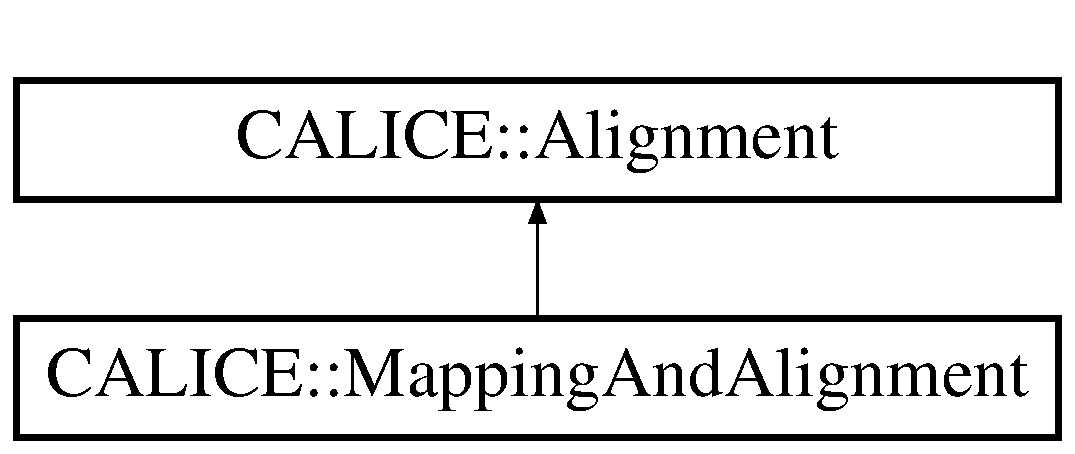
\includegraphics[height=2.000000cm]{classCALICE_1_1Alignment}
\end{center}
\end{figure}
\subsection*{Public Member Functions}
\begin{DoxyCompactItemize}
\item 
{\bf Alignment} ()
\begin{DoxyCompactList}\small\item\em default constructor. \end{DoxyCompactList}\item 
void {\bf init} ()\label{classCALICE_1_1Alignment_adad093be57011962ceaa0dc6fd597759}

\begin{DoxyCompactList}\small\item\em Does nothing for the time being. \end{DoxyCompactList}\item 
U\-Int\-\_\-t {\bf get\-Geometrical\-Cell\-Index} (U\-Int\-\_\-t module\-\_\-index, U\-Int\-\_\-t cell\-\_\-index) const 
\begin{DoxyCompactList}\small\item\em Get the unique cell index of the cell specified by the module and the cell index. \end{DoxyCompactList}\item 
bool {\bf is\-Valid} (U\-Int\-\_\-t module\-\_\-index) const 
\begin{DoxyCompactList}\small\item\em Return true if the type of the given module is valid. \end{DoxyCompactList}\item 
U\-Char\-\_\-t {\bf get\-Module\-Type} (U\-Int\-\_\-t module\-\_\-index) const 
\begin{DoxyCompactList}\small\item\em Get the type of a certain module. \end{DoxyCompactList}\item 
{\bf Three\-Vector\-\_\-t} {\bfseries get\-Position} (U\-Int\-\_\-t module\-\_\-index, U\-Int\-\_\-t cell\-\_\-index) const \label{classCALICE_1_1Alignment_a3ddad6c8a5aeaed18d3529d212d3ba1b}

\item 
{\bf Three\-Vector\-\_\-t} {\bfseries transform\-Position} ({\bf Three\-Vector\-\_\-t} \&a\-\_\-position) const \label{classCALICE_1_1Alignment_a77b2bfc80a819a597a8e451a2bbf7655}

\item 
U\-Int\-\_\-t {\bfseries get\-N\-Modules} () const \label{classCALICE_1_1Alignment_a439df763fea328d7f58336f3b97ca786}

\item 
Bool\-\_\-t {\bf is\-Module} (U\-Int\-\_\-t module\-\_\-index) const \label{classCALICE_1_1Alignment_a4860425f1c86fbc897920647f0dd7451}

\begin{DoxyCompactList}\small\item\em Return false if the module index is out of range. \end{DoxyCompactList}\item 
const {\bf Module\-Description} \& {\bf get\-Module\-Description} (U\-Int\-\_\-t module\-\_\-index) const 
\begin{DoxyCompactList}\small\item\em Return the description object for the given module. \end{DoxyCompactList}\item 
U\-Int\-\_\-t {\bfseries get\-N\-Cells\-Per\-Module} (U\-Int\-\_\-t module\-\_\-index) const \label{classCALICE_1_1Alignment_a67d96a33524e3dd7e4c151943caa103c}

\item 
Float\-\_\-t {\bf get\-Module\-Width} (U\-Int\-\_\-t module\-\_\-index) const \label{classCALICE_1_1Alignment_a2a3b34cd5399e9d4c6c34737314a42e7}

\begin{DoxyCompactList}\small\item\em Get the cell width of the given module and cell. \end{DoxyCompactList}\item 
Float\-\_\-t {\bf get\-Module\-Height} (U\-Int\-\_\-t module\-\_\-index) const \label{classCALICE_1_1Alignment_a5112553b1a361f609e186c85f97d0f7f}

\begin{DoxyCompactList}\small\item\em Get the cell width of the given module and cell. \end{DoxyCompactList}\item 
Float\-\_\-t {\bf get\-Cell\-Width} (U\-Int\-\_\-t module\-\_\-index, U\-Int\-\_\-t cell\-\_\-index) const \label{classCALICE_1_1Alignment_a7ed4ffe8bed99bed35d69c0ac431bc67}

\begin{DoxyCompactList}\small\item\em Get the cell width of the given module and cell. \end{DoxyCompactList}\item 
Float\-\_\-t {\bf get\-Cell\-Height} (U\-Int\-\_\-t module\-\_\-index, U\-Int\-\_\-t cell\-\_\-index) const 
\begin{DoxyCompactList}\small\item\em Get the cell width of the given module. \end{DoxyCompactList}\item 
{\bf Three\-Vector\-\_\-t} {\bf get\-Position} () const \label{classCALICE_1_1Alignment_a8264e5dd81a84e2362f8cc4d26a4c41f}

\begin{DoxyCompactList}\small\item\em Get the position of the detector in its proper coordinate system. \end{DoxyCompactList}\item 
{\bf Three\-Vector\-\_\-t} {\bf get\-Module\-Proper\-Center} (U\-Int\-\_\-t module\-\_\-index) const \label{classCALICE_1_1Alignment_a696dfaa32cdaf473b07c981934598958}

\begin{DoxyCompactList}\small\item\em Get the upper right corner of a module. \end{DoxyCompactList}\item 
{\bf Three\-Vector\-\_\-t} {\bf get\-Module\-Proper\-Position} (U\-Int\-\_\-t module\-\_\-index) const \label{classCALICE_1_1Alignment_ab46ad7e1e3e78dc47fcc4549a231c23e}

\begin{DoxyCompactList}\small\item\em Get the position of a module in the proper coordinate system of the detector. \end{DoxyCompactList}\item 
{\bf Three\-Vector\-\_\-t} {\bf get\-Module\-Position} (U\-Int\-\_\-t module\-\_\-index) const \label{classCALICE_1_1Alignment_a1ecf26def8a818e1f6035c9e18653d28}

\begin{DoxyCompactList}\small\item\em Get the position of a module in the reference coordinate system. \end{DoxyCompactList}\item 
{\bf Three\-Vector\-\_\-t} {\bf get\-Module\-Center} (U\-Int\-\_\-t module\-\_\-index) const \label{classCALICE_1_1Alignment_a4dd6c5cde6371a0b26c6438adf54414f}

\begin{DoxyCompactList}\small\item\em Get the center of a module in the reference coordinate system. \end{DoxyCompactList}\item 
Float\-\_\-t {\bf get\-Detector\-Angle\-Z\-X} () const \label{classCALICE_1_1Alignment_a10d5e1ddf0c26a74421c22774248671d}

\begin{DoxyCompactList}\small\item\em Return the effective rotation angle of the detector. \end{DoxyCompactList}\item 
virtual void {\bf module\-Type\-Changed} (lcio\-::\-L\-C\-Collection $\ast$col)
\begin{DoxyCompactList}\small\item\em Inform the object about changes of the module types. \end{DoxyCompactList}\item 
virtual void {\bf module\-Location\-Changed} (lcio\-::\-L\-C\-Collection $\ast$col)
\begin{DoxyCompactList}\small\item\em Inform the object about changes of the module locations. \end{DoxyCompactList}\item 
virtual void {\bf stage\-Position\-Changed} (lcio\-::\-L\-C\-Collection $\ast$col)
\begin{DoxyCompactList}\small\item\em Inform the object about changes in the stage positions on which the detector is mounted. \end{DoxyCompactList}\item 
virtual void {\bf detector\-Transformation} (lcio\-::\-L\-C\-Collection $\ast$col)
\begin{DoxyCompactList}\small\item\em Inform the object about changes of the detector position and rotation. \end{DoxyCompactList}\item 
virtual void {\bf reference\-Transformation} (lcio\-::\-L\-C\-Collection $\ast$col)
\begin{DoxyCompactList}\small\item\em Inform the object about changes of the reference position and rotation. \end{DoxyCompactList}\item 
U\-Int\-\_\-t {\bf get\-Cell\-Index\-Offset} (U\-Int\-\_\-t module\-\_\-index) const \label{classCALICE_1_1Alignment_ad07573bf525c2271792bc040242632a2}

\begin{DoxyCompactList}\small\item\em Get the cell index offset of a module. \end{DoxyCompactList}\end{DoxyCompactItemize}
\subsection*{Protected Types}
\begin{DoxyCompactItemize}
\item 
typedef {\bf Simple\-Array\-\_\-t}$<$ pair\\*
$<$ U\-Int\-\_\-t, {\bf Module\-Location} $>$ $>$ {\bf Module\-List\-\_\-t}
\begin{DoxyCompactList}\small\item\em Defined module locations (not necessarily connected to a front-\/end. \end{DoxyCompactList}\item 
typedef {\bf Simple\-Array\-\_\-t}\\*
$<$ {\bf Module\-Description} $>$ {\bfseries Module\-Type\-List\-\_\-t}\label{classCALICE_1_1Alignment_a10d63d19612d0b5384bfc7f9b7f84bbd}

\end{DoxyCompactItemize}
\subsection*{Protected Attributes}
\begin{DoxyCompactItemize}
\item 
{\bf Module\-List\-\_\-t} {\bfseries \-\_\-module\-Location\-List}\label{classCALICE_1_1Alignment_a7038cce4a5b2baf25597867f0b5407c5}

\item 
{\bf Module\-Type\-List\-\_\-t} {\bfseries \-\_\-module\-Type\-List}\label{classCALICE_1_1Alignment_a975a8333c0f374f44dee0fa6c37cf732}

\end{DoxyCompactItemize}
\subsection*{Private Types}
\begin{DoxyCompactItemize}
\item 
enum {\bfseries E\-Transformation} \{ {\bfseries k\-Detector}, 
{\bfseries k\-Reference}, 
{\bfseries k\-Effective}, 
{\bfseries k\-N\-Transformations}
 \}
\item 
typedef void(Alignment\-::$\ast$ {\bf Stage\-Change\-Handle\-Func\-\_\-t} )(lcio\-::\-L\-C\-Collection $\ast$col)\label{classCALICE_1_1Alignment_a5131ddec8fd42fefa45de5826aecd4c1}

\begin{DoxyCompactList}\small\item\em A map which holds pointers to functions to access the parameters of teh movable stage(s) \end{DoxyCompactList}\end{DoxyCompactItemize}
\subsection*{Private Member Functions}
\begin{DoxyCompactItemize}
\item 
void {\bf set\-Transformation} (lcio\-::\-L\-C\-Collection $\ast$col, E\-Transformation transformation\-\_\-type)\label{classCALICE_1_1Alignment_adb7fd43e529d374f41e8be0a1610faf9}

\begin{DoxyCompactList}\small\item\em Set the transformation parameters from the conditions data collection. \end{DoxyCompactList}\item 
void {\bf calculate\-Effective\-Transformation} ()
\begin{DoxyCompactList}\small\item\em Calculate the effective transformation from the detector and reference transformation. \end{DoxyCompactList}\item 
void {\bfseries handle\-Emc\-Stage} (L\-C\-Collection $\ast$)\label{classCALICE_1_1Alignment_abf5097c7e86a04e285cd59ddf8848c47}

\item 
void {\bfseries handle\-Ahc\-Stage} (L\-C\-Collection $\ast$)\label{classCALICE_1_1Alignment_a907fd80bfc25e5f98b6ebab3fb7533fa}

\end{DoxyCompactItemize}
\subsection*{Private Attributes}
\begin{DoxyCompactItemize}
\item 
Float\-\_\-t {\bf \-\_\-detector\-Pos} [k\-N\-Transformations][3]\label{classCALICE_1_1Alignment_a6f73f5a4df2e1b7fd2a3da7c99d70d51}

\begin{DoxyCompactList}\small\item\em the position of the detector \end{DoxyCompactList}\item 
Float\-\_\-t {\bf \-\_\-detector\-Angle\-Z\-X} [k\-N\-Transformations]
\begin{DoxyCompactList}\small\item\em configuration angle w.\-r.\-t. \end{DoxyCompactList}\item 
Double\-\_\-t {\bf \-\_\-detector\-Angle\-Z\-X\-Sin}\label{classCALICE_1_1Alignment_a398120953f6f68d96563c57dd95e12aa}

\begin{DoxyCompactList}\small\item\em sin of the effective rotation angle in the z-\/x plane \end{DoxyCompactList}\item 
Double\-\_\-t {\bf \-\_\-detector\-Angle\-Z\-X\-Cos}\label{classCALICE_1_1Alignment_a4b7a1cc57b53c53a0f251dae7782f675}

\begin{DoxyCompactList}\small\item\em cos of the effective rotation angle in the z-\/x plane \end{DoxyCompactList}\item 
Float\-\_\-t {\bf \-\_\-detector\-Rotation\-X0} [k\-N\-Transformations]\label{classCALICE_1_1Alignment_a5b7bee79b2ad35a2e7b128f841a1fd64}

\begin{DoxyCompactList}\small\item\em origin of the detector ratation (x-\/direction) \end{DoxyCompactList}\item 
Float\-\_\-t {\bf \-\_\-detector\-Rotation\-Z0} [k\-N\-Transformations]\label{classCALICE_1_1Alignment_a2faba0894844b8779abd31d7e8a56854}

\begin{DoxyCompactList}\small\item\em origin of the detector ratation (z-\/direction) \end{DoxyCompactList}\item 
std\-::map$<$ std\-::string, \\*
{\bf Stage\-Change\-Handle\-Func\-\_\-t} $>$ {\bfseries \-\_\-known\-Stage\-Types}\label{classCALICE_1_1Alignment_a3b409667846fdd3b1b36abca4e74ba8d}

\item 
float {\bf \-\_\-stage\-Offset\-\_\-x}\label{classCALICE_1_1Alignment_a38bc228c141775137178ab1c171a4c92}

\begin{DoxyCompactList}\small\item\em The offsets due to the movable stage. \end{DoxyCompactList}\item 
float {\bfseries \-\_\-stage\-Offset\-\_\-y}\label{classCALICE_1_1Alignment_a734151cd0b80de77cd16cce5b7ae9106}

\end{DoxyCompactItemize}
\subsection*{Static Private Attributes}
\begin{DoxyCompactItemize}
\item 
static const Double\-\_\-t {\bfseries \-\_\-\-\_\-deg\-To\-Rad} =M\-\_\-\-P\-I/180.\label{classCALICE_1_1Alignment_af48cedd060a33b725e5f14f81f3033d1}

\end{DoxyCompactItemize}


\subsection{Detailed Description}
Class to comunicate/handle the translation into unique layer/cell ids and 3\-D spacial coordinates. 

The class has to be informed about changes of the detector configuration using the methods \doxyref{C\-A\-L\-I\-C\-E\-::\-Alignment\-::module\-Type\-Changed}{p.}{classCALICE_1_1Alignment_adc041696a184db384a57bca51df7bc25}, \doxyref{C\-A\-L\-I\-C\-E\-::\-Alignment\-::module\-Location\-Changed}{p.}{classCALICE_1_1Alignment_a3ea188d0a90c7e0881d735cf55ef5604}, \doxyref{C\-A\-L\-I\-C\-E\-::\-Mapping\-And\-Alignment\-::module\-Connection\-Changed}{p.}{classCALICE_1_1MappingAndAlignment_a3717c2ea27a5a60ff2a41d17803ff148} and Alignment\-::experimental\-Setup. This information is used to map the D\-A\-Q signals to cells and calculate 3\-D spacial coordinates for hits.

The class performs range checks only if B\-O\-U\-N\-D\-A\-R\-Y\-\_\-\-C\-H\-E\-C\-K is defined. 

Definition at line 42 of file Alignment.\-hh.



\subsection{Member Typedef Documentation}
\index{C\-A\-L\-I\-C\-E\-::\-Alignment@{C\-A\-L\-I\-C\-E\-::\-Alignment}!Module\-List\-\_\-t@{Module\-List\-\_\-t}}
\index{Module\-List\-\_\-t@{Module\-List\-\_\-t}!CALICE::Alignment@{C\-A\-L\-I\-C\-E\-::\-Alignment}}
\subsubsection[{Module\-List\-\_\-t}]{\setlength{\rightskip}{0pt plus 5cm}typedef {\bf Simple\-Array\-\_\-t}$<$pair$<$U\-Int\-\_\-t,{\bf Module\-Location}$>$ $>$ {\bf C\-A\-L\-I\-C\-E\-::\-Alignment\-::\-Module\-List\-\_\-t}\hspace{0.3cm}{\ttfamily [protected]}}\label{classCALICE_1_1Alignment_ad0153c70861a5bc9976bc21983ac319f}


Defined module locations (not necessarily connected to a front-\/end. 

First component contains the module I\-D, the second the module location information. 

Definition at line 475 of file Alignment.\-hh.



\subsection{Constructor \& Destructor Documentation}
\index{C\-A\-L\-I\-C\-E\-::\-Alignment@{C\-A\-L\-I\-C\-E\-::\-Alignment}!Alignment@{Alignment}}
\index{Alignment@{Alignment}!CALICE::Alignment@{C\-A\-L\-I\-C\-E\-::\-Alignment}}
\subsubsection[{Alignment}]{\setlength{\rightskip}{0pt plus 5cm}C\-A\-L\-I\-C\-E\-::\-Alignment\-::\-Alignment (
\begin{DoxyParamCaption}
{}
\end{DoxyParamCaption}
)}\label{classCALICE_1_1Alignment_a9301ea57c3cf0bf16154f67e45023385}


default constructor. 

The default constructor configures the conditions data change delegators. 

Definition at line 29 of file Alignment.\-cc.



References set\-Transformation().



\subsection{Member Function Documentation}
\index{C\-A\-L\-I\-C\-E\-::\-Alignment@{C\-A\-L\-I\-C\-E\-::\-Alignment}!calculate\-Effective\-Transformation@{calculate\-Effective\-Transformation}}
\index{calculate\-Effective\-Transformation@{calculate\-Effective\-Transformation}!CALICE::Alignment@{C\-A\-L\-I\-C\-E\-::\-Alignment}}
\subsubsection[{calculate\-Effective\-Transformation}]{\setlength{\rightskip}{0pt plus 5cm}void C\-A\-L\-I\-C\-E\-::\-Alignment\-::calculate\-Effective\-Transformation (
\begin{DoxyParamCaption}
{}
\end{DoxyParamCaption}
)\hspace{0.3cm}{\ttfamily [private]}}\label{classCALICE_1_1Alignment_af778a021450c0087cbf459eb291aa8f1}


Calculate the effective transformation from the detector and reference transformation. 



Definition at line 171 of file Alignment.\-cc.



References \-\_\-detector\-Angle\-Z\-X, \-\_\-detector\-Angle\-Z\-X\-Cos, \-\_\-detector\-Angle\-Z\-X\-Sin, \-\_\-detector\-Pos, \-\_\-detector\-Rotation\-X0, and \-\_\-detector\-Rotation\-Z0.



Referenced by set\-Transformation().

\index{C\-A\-L\-I\-C\-E\-::\-Alignment@{C\-A\-L\-I\-C\-E\-::\-Alignment}!detector\-Transformation@{detector\-Transformation}}
\index{detector\-Transformation@{detector\-Transformation}!CALICE::Alignment@{C\-A\-L\-I\-C\-E\-::\-Alignment}}
\subsubsection[{detector\-Transformation}]{\setlength{\rightskip}{0pt plus 5cm}virtual void C\-A\-L\-I\-C\-E\-::\-Alignment\-::detector\-Transformation (
\begin{DoxyParamCaption}
\item[{lcio\-::\-L\-C\-Collection $\ast$}]{col}
\end{DoxyParamCaption}
)\hspace{0.3cm}{\ttfamily [inline]}, {\ttfamily [virtual]}}\label{classCALICE_1_1Alignment_a85a9ad1e7e95e2ade18f30e6373eadfa}


Inform the object about changes of the detector position and rotation. 


\begin{DoxyParams}{Parameters}
{\em col} & collection of \doxyref{Detector\-Transformation}{p.}{classCALICE_1_1DetectorTransformation} objects This class must be called before querying the postion of cells. The position is calculated in the reference coorindate system. \\
\hline
\end{DoxyParams}


Definition at line 457 of file Alignment.\-hh.

\index{C\-A\-L\-I\-C\-E\-::\-Alignment@{C\-A\-L\-I\-C\-E\-::\-Alignment}!get\-Cell\-Height@{get\-Cell\-Height}}
\index{get\-Cell\-Height@{get\-Cell\-Height}!CALICE::Alignment@{C\-A\-L\-I\-C\-E\-::\-Alignment}}
\subsubsection[{get\-Cell\-Height}]{\setlength{\rightskip}{0pt plus 5cm}Float\-\_\-t C\-A\-L\-I\-C\-E\-::\-Alignment\-::get\-Cell\-Height (
\begin{DoxyParamCaption}
\item[{U\-Int\-\_\-t}]{module\-\_\-index, }
\item[{U\-Int\-\_\-t}]{cell\-\_\-index}
\end{DoxyParamCaption}
) const\hspace{0.3cm}{\ttfamily [inline]}}\label{classCALICE_1_1Alignment_a84ad3b3ffba7850de98971a51eeba82f}


Get the cell width of the given module. 

It is assumed that the cells of one module all have the same width. 

Definition at line 325 of file Alignment.\-hh.

\index{C\-A\-L\-I\-C\-E\-::\-Alignment@{C\-A\-L\-I\-C\-E\-::\-Alignment}!get\-Geometrical\-Cell\-Index@{get\-Geometrical\-Cell\-Index}}
\index{get\-Geometrical\-Cell\-Index@{get\-Geometrical\-Cell\-Index}!CALICE::Alignment@{C\-A\-L\-I\-C\-E\-::\-Alignment}}
\subsubsection[{get\-Geometrical\-Cell\-Index}]{\setlength{\rightskip}{0pt plus 5cm}U\-Int\-\_\-t C\-A\-L\-I\-C\-E\-::\-Alignment\-::get\-Geometrical\-Cell\-Index (
\begin{DoxyParamCaption}
\item[{U\-Int\-\_\-t}]{module\-\_\-index, }
\item[{U\-Int\-\_\-t}]{cell\-\_\-index}
\end{DoxyParamCaption}
) const\hspace{0.3cm}{\ttfamily [inline]}}\label{classCALICE_1_1Alignment_add6b290637455010456ce6f643ccb34f}


Get the unique cell index of the cell specified by the module and the cell index. 


\begin{DoxyParams}{Parameters}
{\em module\-\_\-index} & unique index for modules which should run from 0..total number of modules \\
\hline
{\em cell\-\_\-index} & within the module (0.. number of cells of this module type) \\
\hline
\end{DoxyParams}
\begin{DoxyReturn}{Returns}
unique cell index. 
\end{DoxyReturn}

\begin{DoxyExceptions}{Exceptions}
{\em range\-\_\-error} & if the module index is out of range and B\-O\-U\-N\-D\-A\-R\-Y\-\_\-\-C\-H\-E\-C\-K is defined\\
\hline
\end{DoxyExceptions}
The cell index conforms to the Mokka specification (see for example \doxyref{Cell\-Index}{p.}{classCALICE_1_1CellIndex}). It is composed of the layer number, the wafer column and row, and the pad column and row. 

Definition at line 68 of file Alignment.\-hh.

\index{C\-A\-L\-I\-C\-E\-::\-Alignment@{C\-A\-L\-I\-C\-E\-::\-Alignment}!get\-Module\-Description@{get\-Module\-Description}}
\index{get\-Module\-Description@{get\-Module\-Description}!CALICE::Alignment@{C\-A\-L\-I\-C\-E\-::\-Alignment}}
\subsubsection[{get\-Module\-Description}]{\setlength{\rightskip}{0pt plus 5cm}const {\bf Module\-Description}\& C\-A\-L\-I\-C\-E\-::\-Alignment\-::get\-Module\-Description (
\begin{DoxyParamCaption}
\item[{U\-Int\-\_\-t}]{module\-\_\-index}
\end{DoxyParamCaption}
) const\hspace{0.3cm}{\ttfamily [inline]}}\label{classCALICE_1_1Alignment_a6ac1899ddab2b35464b85ec39a67ede7}


Return the description object for the given module. 


\begin{DoxyParams}{Parameters}
{\em module\-\_\-index} & the index of the moduel. \\
\hline
\end{DoxyParams}


Definition at line 229 of file Alignment.\-hh.

\index{C\-A\-L\-I\-C\-E\-::\-Alignment@{C\-A\-L\-I\-C\-E\-::\-Alignment}!get\-Module\-Type@{get\-Module\-Type}}
\index{get\-Module\-Type@{get\-Module\-Type}!CALICE::Alignment@{C\-A\-L\-I\-C\-E\-::\-Alignment}}
\subsubsection[{get\-Module\-Type}]{\setlength{\rightskip}{0pt plus 5cm}U\-Char\-\_\-t C\-A\-L\-I\-C\-E\-::\-Alignment\-::get\-Module\-Type (
\begin{DoxyParamCaption}
\item[{U\-Int\-\_\-t}]{module\-\_\-index}
\end{DoxyParamCaption}
) const\hspace{0.3cm}{\ttfamily [inline]}}\label{classCALICE_1_1Alignment_a6347626acbfc5dfcbca3c97c89fcad70}


Get the type of a certain module. 

The module type together with the module I\-D uniquly identifies a module. Different modules of one type always have different I\-Ds but modules of different types may have the same I\-D. In case of the E\-C\-A\-L the module I\-D is the serial number of the P\-C\-Bs. 
\begin{DoxyParams}{Parameters}
{\em module\-\_\-index} & the index of the module within the detector (not necessarily the same as the module I\-D) \\
\hline
\end{DoxyParams}
\begin{DoxyReturn}{Returns}
the module type 
\end{DoxyReturn}

\begin{DoxyExceptions}{Exceptions}
{\em range\-\_\-error} & if the module specified by module\-\_\-index is not defined but only if B\-O\-U\-N\-D\-A\-R\-Y\-\_\-\-C\-H\-E\-C\-K is defined. \\
\hline
\end{DoxyExceptions}
\begin{DoxySeeAlso}{See Also}
get\-Module\-I\-D() 
\end{DoxySeeAlso}


Definition at line 114 of file Alignment.\-hh.



Referenced by C\-A\-L\-I\-C\-E\-::\-Mapping\-And\-Alignment\-::print().

\index{C\-A\-L\-I\-C\-E\-::\-Alignment@{C\-A\-L\-I\-C\-E\-::\-Alignment}!is\-Valid@{is\-Valid}}
\index{is\-Valid@{is\-Valid}!CALICE::Alignment@{C\-A\-L\-I\-C\-E\-::\-Alignment}}
\subsubsection[{is\-Valid}]{\setlength{\rightskip}{0pt plus 5cm}bool C\-A\-L\-I\-C\-E\-::\-Alignment\-::is\-Valid (
\begin{DoxyParamCaption}
\item[{U\-Int\-\_\-t}]{module\-\_\-index}
\end{DoxyParamCaption}
) const\hspace{0.3cm}{\ttfamily [inline]}}\label{classCALICE_1_1Alignment_a3b3a82a744ce67860086203baef3ddff}


Return true if the type of the given module is valid. 


\begin{DoxyParams}{Parameters}
{\em module\-\_\-index} & the index of the given module. \\
\hline
\end{DoxyParams}


Definition at line 90 of file Alignment.\-hh.



Referenced by C\-A\-L\-I\-C\-E\-::\-Mapping\-And\-Alignment\-::print().

\index{C\-A\-L\-I\-C\-E\-::\-Alignment@{C\-A\-L\-I\-C\-E\-::\-Alignment}!module\-Location\-Changed@{module\-Location\-Changed}}
\index{module\-Location\-Changed@{module\-Location\-Changed}!CALICE::Alignment@{C\-A\-L\-I\-C\-E\-::\-Alignment}}
\subsubsection[{module\-Location\-Changed}]{\setlength{\rightskip}{0pt plus 5cm}void C\-A\-L\-I\-C\-E\-::\-Alignment\-::module\-Location\-Changed (
\begin{DoxyParamCaption}
\item[{lcio\-::\-L\-C\-Collection $\ast$}]{col}
\end{DoxyParamCaption}
)\hspace{0.3cm}{\ttfamily [virtual]}}\label{classCALICE_1_1Alignment_a3ea188d0a90c7e0881d735cf55ef5604}


Inform the object about changes of the module locations. 


\begin{DoxyParams}{Parameters}
{\em col} & collection of \doxyref{Module\-Location}{p.}{classCALICE_1_1ModuleLocation} objects This class must be called before using any(most) of the other methods. The function call will cause a rebuild of the module D\-A\-Q front-\/end connection tree. \\
\hline
\end{DoxyParams}


Reimplemented in {\bf C\-A\-L\-I\-C\-E\-::\-Mapping\-And\-Alignment} \doxyref{}{p.}{classCALICE_1_1MappingAndAlignment_ab9d17873aeb090388556547cb6b67ba8}.



Definition at line 76 of file Alignment.\-cc.



Referenced by C\-A\-L\-I\-C\-E\-::\-Mapping\-And\-Alignment\-::module\-Location\-Changed().

\index{C\-A\-L\-I\-C\-E\-::\-Alignment@{C\-A\-L\-I\-C\-E\-::\-Alignment}!module\-Type\-Changed@{module\-Type\-Changed}}
\index{module\-Type\-Changed@{module\-Type\-Changed}!CALICE::Alignment@{C\-A\-L\-I\-C\-E\-::\-Alignment}}
\subsubsection[{module\-Type\-Changed}]{\setlength{\rightskip}{0pt plus 5cm}void C\-A\-L\-I\-C\-E\-::\-Alignment\-::module\-Type\-Changed (
\begin{DoxyParamCaption}
\item[{lcio\-::\-L\-C\-Collection $\ast$}]{col}
\end{DoxyParamCaption}
)\hspace{0.3cm}{\ttfamily [virtual]}}\label{classCALICE_1_1Alignment_adc041696a184db384a57bca51df7bc25}


Inform the object about changes of the module types. 


\begin{DoxyParams}{Parameters}
{\em col} & collection of \doxyref{Module\-Description}{p.}{classCALICE_1_1ModuleDescription} objects This class must be called before using any(most) of the other methods. The function call will cause a rebuild of the module D\-A\-Q front-\/end connection tree. \\
\hline
\end{DoxyParams}


Reimplemented in {\bf C\-A\-L\-I\-C\-E\-::\-Mapping\-And\-Alignment} \doxyref{}{p.}{classCALICE_1_1MappingAndAlignment_a5564c399de481a023b702a39a04fea7f}.



Definition at line 47 of file Alignment.\-cc.



Referenced by C\-A\-L\-I\-C\-E\-::\-Mapping\-And\-Alignment\-::module\-Type\-Changed().

\index{C\-A\-L\-I\-C\-E\-::\-Alignment@{C\-A\-L\-I\-C\-E\-::\-Alignment}!reference\-Transformation@{reference\-Transformation}}
\index{reference\-Transformation@{reference\-Transformation}!CALICE::Alignment@{C\-A\-L\-I\-C\-E\-::\-Alignment}}
\subsubsection[{reference\-Transformation}]{\setlength{\rightskip}{0pt plus 5cm}virtual void C\-A\-L\-I\-C\-E\-::\-Alignment\-::reference\-Transformation (
\begin{DoxyParamCaption}
\item[{lcio\-::\-L\-C\-Collection $\ast$}]{col}
\end{DoxyParamCaption}
)\hspace{0.3cm}{\ttfamily [inline]}, {\ttfamily [virtual]}}\label{classCALICE_1_1Alignment_aedf5694bbb286510411e1de986e51ac5}


Inform the object about changes of the reference position and rotation. 


\begin{DoxyParams}{Parameters}
{\em col} & collection of \doxyref{Detector\-Transformation}{p.}{classCALICE_1_1DetectorTransformation} objects This class must be called before querying the postion of cells. The position is calculated in the reference coordinate system. \\
\hline
\end{DoxyParams}


Definition at line 466 of file Alignment.\-hh.

\index{C\-A\-L\-I\-C\-E\-::\-Alignment@{C\-A\-L\-I\-C\-E\-::\-Alignment}!stage\-Position\-Changed@{stage\-Position\-Changed}}
\index{stage\-Position\-Changed@{stage\-Position\-Changed}!CALICE::Alignment@{C\-A\-L\-I\-C\-E\-::\-Alignment}}
\subsubsection[{stage\-Position\-Changed}]{\setlength{\rightskip}{0pt plus 5cm}void C\-A\-L\-I\-C\-E\-::\-Alignment\-::stage\-Position\-Changed (
\begin{DoxyParamCaption}
\item[{lcio\-::\-L\-C\-Collection $\ast$}]{col}
\end{DoxyParamCaption}
)\hspace{0.3cm}{\ttfamily [virtual]}}\label{classCALICE_1_1Alignment_ab018d115126785360ec8e70fb710409b}


Inform the object about changes in the stage positions on which the detector is mounted. 


\begin{DoxyParams}{Parameters}
{\em col} & collection of Stage\-Parameters objects This class must be called before calculating the actual cell positions The function will provide the xy values for a correct transversal alignment of the detectors. \\
\hline
\end{DoxyParams}


Definition at line 218 of file Alignment.\-cc.



\subsection{Field Documentation}
\index{C\-A\-L\-I\-C\-E\-::\-Alignment@{C\-A\-L\-I\-C\-E\-::\-Alignment}!\-\_\-detector\-Angle\-Z\-X@{\-\_\-detector\-Angle\-Z\-X}}
\index{\-\_\-detector\-Angle\-Z\-X@{\-\_\-detector\-Angle\-Z\-X}!CALICE::Alignment@{C\-A\-L\-I\-C\-E\-::\-Alignment}}
\subsubsection[{\-\_\-detector\-Angle\-Z\-X}]{\setlength{\rightskip}{0pt plus 5cm}Float\-\_\-t C\-A\-L\-I\-C\-E\-::\-Alignment\-::\-\_\-detector\-Angle\-Z\-X[k\-N\-Transformations]\hspace{0.3cm}{\ttfamily [private]}}\label{classCALICE_1_1Alignment_a7580f22b535e4538967b0ef80f22f3ed}


configuration angle w.\-r.\-t. 

to the beam axis in the horizontal plane 

Definition at line 501 of file Alignment.\-hh.



Referenced by calculate\-Effective\-Transformation(), and set\-Transformation().



The documentation for this class was generated from the following files\-:\begin{DoxyCompactItemize}
\item 
Alignment.\-hh\item 
Alignment.\-cc\end{DoxyCompactItemize}

\section{Average\-\_\-t Class Reference}
\label{classAverage__t}\index{Average\-\_\-t@{Average\-\_\-t}}


Calculate mean and standard deviation and find minimum and maximum value.  




{\ttfamily \#include $<$Average\-\_\-t.\-hh$>$}

\subsection*{Public Member Functions}
\begin{DoxyCompactItemize}
\item 
{\bf Average\-\_\-t} ()\label{classAverage__t_aa221818a7a022083297e9cab811252e6}

\begin{DoxyCompactList}\small\item\em Default constructor initialses all arrays to be ready to gather statastics of a variable. \end{DoxyCompactList}\item 
void {\bf add} (Float\-\_\-t value, Float\-\_\-t {\bf weight}=1.)
\begin{DoxyCompactList}\small\item\em Build the sum and the sum of squares and find the minimum and maximum value. \end{DoxyCompactList}\item 
void {\bf calculate} ()
\begin{DoxyCompactList}\small\item\em Calculate the standard deviation and the mean. \end{DoxyCompactList}\item 
Double\-\_\-t {\bf mean} () const 
\begin{DoxyCompactList}\small\item\em Return the mean value. \end{DoxyCompactList}\item 
Double\-\_\-t {\bf sigma} () const 
\begin{DoxyCompactList}\small\item\em Return the standard deviation. \end{DoxyCompactList}\item 
Float\-\_\-t {\bf min} () const \label{classAverage__t_a7ca3e52df15cd84cd40b8456f3d505e8}

\begin{DoxyCompactList}\small\item\em Return the minimum value. \end{DoxyCompactList}\item 
Float\-\_\-t {\bf max} () const \label{classAverage__t_a1cfde99d82e467a5f6adf92d51955225}

\begin{DoxyCompactList}\small\item\em Return the maximum value. \end{DoxyCompactList}\item 
Double\-\_\-t {\bf weight} () const \label{classAverage__t_a3c8ebca4ecd924335737f7aacef198f7}

\begin{DoxyCompactList}\small\item\em Get the total accumulated weight. \end{DoxyCompactList}\item 
Double\-\_\-t {\bf sum} () const \label{classAverage__t_aeb4e2a1c2ddac4ed9cc055689c911a49}

\begin{DoxyCompactList}\small\item\em Get the total accumulated data. \end{DoxyCompactList}\end{DoxyCompactItemize}
\subsection*{Protected Attributes}
\begin{DoxyCompactItemize}
\item 
Double\-\_\-t {\bfseries \-\_\-weight}\label{classAverage__t_ae8fffd362517a4498e222a7c4c4dc158}

\item 
Float\-\_\-t {\bfseries \-\_\-min}\label{classAverage__t_a6fa8a684525c545162a09e4c8da6849c}

\item 
Float\-\_\-t {\bfseries \-\_\-max}\label{classAverage__t_ae1698dbafedc10f4bec7425fe6f2a89d}

\item 
\begin{tabbing}
xx\=xx\=xx\=xx\=xx\=xx\=xx\=xx\=xx\=\kill
union \{\\
\>Double\_t {\bfseries \_sum}\\
\>Double\_t {\bfseries \_mean}\\
\}; \label{classAverage__t_ad694cc340eea19e0c4c7e3085a689214}
\\

\end{tabbing}\item 
\begin{tabbing}
xx\=xx\=xx\=xx\=xx\=xx\=xx\=xx\=xx\=\kill
union \{\\
\>Double\_t {\bfseries \_sum2}\\
\>Double\_t {\bfseries \_sigma}\\
\}; \label{classAverage__t_ae244c1ec670e1edbbcf64f0d79e4780e}
\\

\end{tabbing}\end{DoxyCompactItemize}
\subsection*{Friends}
\begin{DoxyCompactItemize}
\item 
std\-::ostream \& {\bfseries operator$<$$<$} (std\-::ostream \&os, const {\bf Average\-\_\-t} \&a)\label{classAverage__t_ae983d5da007094c692f583fd58af1bfb}

\end{DoxyCompactItemize}


\subsection{Detailed Description}
Calculate mean and standard deviation and find minimum and maximum value. 

The minimum and maximum is not searched/memorised if A\-V\-E\-R\-A\-G\-E\-\_\-\-W\-I\-T\-H\-O\-U\-T\-\_\-\-M\-I\-N\-\_\-\-M\-A\-X is defined. 

Definition at line 21 of file Average\-\_\-t.\-hh.



\subsection{Member Function Documentation}
\index{Average\-\_\-t@{Average\-\_\-t}!add@{add}}
\index{add@{add}!Average_t@{Average\-\_\-t}}
\subsubsection[{add}]{\setlength{\rightskip}{0pt plus 5cm}void Average\-\_\-t\-::add (
\begin{DoxyParamCaption}
\item[{Float\-\_\-t}]{value, }
\item[{Float\-\_\-t}]{weight = {\ttfamily 1.}}
\end{DoxyParamCaption}
)\hspace{0.3cm}{\ttfamily [inline]}}\label{classAverage__t_a1dc4d4d78f339ff9025acf6ac756636e}


Build the sum and the sum of squares and find the minimum and maximum value. 

The sums can be used later to calculate the mean and the standard deviation 
\begin{DoxyParams}{Parameters}
{\em value} & the value to be added to the sum and the sum of squares \\
\hline
{\em weight} & the weight given to this value in the sums. (\\
\hline
\end{DoxyParams}
\begin{DoxySeeAlso}{See Also}
\doxyref{calculate}{p.}{classAverage__t_a4b49c45f3da3c5761ba355508a42b3ef}) 
\end{DoxySeeAlso}


Definition at line 39 of file Average\-\_\-t.\-hh.



References weight().

\index{Average\-\_\-t@{Average\-\_\-t}!calculate@{calculate}}
\index{calculate@{calculate}!Average_t@{Average\-\_\-t}}
\subsubsection[{calculate}]{\setlength{\rightskip}{0pt plus 5cm}void Average\-\_\-t\-::calculate (
\begin{DoxyParamCaption}
{}
\end{DoxyParamCaption}
)\hspace{0.3cm}{\ttfamily [inline]}}\label{classAverage__t_a4b49c45f3da3c5761ba355508a42b3ef}


Calculate the standard deviation and the mean. 

The mean and the standard deviation are stored in the locations which are also used for the sums. Therefore if further values are added after \doxyref{calculate()}{p.}{classAverage__t_a4b49c45f3da3c5761ba355508a42b3ef} was called, the result is undefined. 

Definition at line 51 of file Average\-\_\-t.\-hh.



References mean(), and sigma().

\index{Average\-\_\-t@{Average\-\_\-t}!mean@{mean}}
\index{mean@{mean}!Average_t@{Average\-\_\-t}}
\subsubsection[{mean}]{\setlength{\rightskip}{0pt plus 5cm}Double\-\_\-t Average\-\_\-t\-::mean (
\begin{DoxyParamCaption}
{}
\end{DoxyParamCaption}
) const\hspace{0.3cm}{\ttfamily [inline]}}\label{classAverage__t_a7674fd214ab308cb48605190413762b4}


Return the mean value. 

returns only a correct result after at least 1 value was added and calculate was called. 

Definition at line 63 of file Average\-\_\-t.\-hh.



Referenced by calculate().

\index{Average\-\_\-t@{Average\-\_\-t}!sigma@{sigma}}
\index{sigma@{sigma}!Average_t@{Average\-\_\-t}}
\subsubsection[{sigma}]{\setlength{\rightskip}{0pt plus 5cm}Double\-\_\-t Average\-\_\-t\-::sigma (
\begin{DoxyParamCaption}
{}
\end{DoxyParamCaption}
) const\hspace{0.3cm}{\ttfamily [inline]}}\label{classAverage__t_afdab526173bec21760599ef1183f5d05}


Return the standard deviation. 

returns only a correct result after at least 1 value was added and calculate was called. 

Definition at line 68 of file Average\-\_\-t.\-hh.



Referenced by calculate().



The documentation for this class was generated from the following file\-:\begin{DoxyCompactItemize}
\item 
Average\-\_\-t.\-hh\end{DoxyCompactItemize}

\section{Average\-Simple\-\_\-t Class Reference}
\label{classAverageSimple__t}\index{Average\-Simple\-\_\-t@{Average\-Simple\-\_\-t}}


Calculate mean and standard deviation.  




{\ttfamily \#include $<$Average\-Simple\-\_\-t.\-hh$>$}

\subsection*{Public Member Functions}
\begin{DoxyCompactItemize}
\item 
{\bf Average\-Simple\-\_\-t} ()\label{classAverageSimple__t_ae833f15db3394a0815c3ff9cf2930a83}

\begin{DoxyCompactList}\small\item\em Default constructor initialses all arrays to be ready to gather statastics of a variable. \end{DoxyCompactList}\item 
void {\bf add} (Float\-\_\-t value)
\begin{DoxyCompactList}\small\item\em build the sum and the sum of squares. \end{DoxyCompactList}\item 
void {\bf calculate} ()
\begin{DoxyCompactList}\small\item\em calculate the standard deviation and the mean. \end{DoxyCompactList}\item 
Double\-\_\-t {\bf mean} () const 
\begin{DoxyCompactList}\small\item\em return the mean value. \end{DoxyCompactList}\item 
Double\-\_\-t {\bf sigma} () const 
\begin{DoxyCompactList}\small\item\em return the standard deviation. \end{DoxyCompactList}\item 
U\-Int\-\_\-t {\bf n} () const \label{classAverageSimple__t_a7cc2397693a23fbdfe17bb47e1db2242}

\begin{DoxyCompactList}\small\item\em return the sample size. \end{DoxyCompactList}\item 
Double\-\_\-t {\bf sum} () const \label{classAverageSimple__t_aef347ef1de5a8fbbf05e2e8dc58706b9}

\begin{DoxyCompactList}\small\item\em Get the total accumulated data. \end{DoxyCompactList}\item 
void {\bfseries operator+=} (Float\-\_\-t val)\label{classAverageSimple__t_add61dc4626c1add4679a8fa3339587f9}

\end{DoxyCompactItemize}
\subsection*{Protected Attributes}
\begin{DoxyCompactItemize}
\item 
U\-Int\-\_\-t {\bfseries \-\_\-n}\label{classAverageSimple__t_ae9f5cf86663225669d2e41907be9e82a}

\item 
\begin{tabbing}
xx\=xx\=xx\=xx\=xx\=xx\=xx\=xx\=xx\=\kill
union \{\\
\>Double\_t {\bfseries \_sum}\\
\>Double\_t {\bfseries \_mean}\\
\}; \label{classAverageSimple__t_acf269ad62ad8de3768972f6af1806b85}
\\

\end{tabbing}\item 
\begin{tabbing}
xx\=xx\=xx\=xx\=xx\=xx\=xx\=xx\=xx\=\kill
union \{\\
\>Double\_t {\bfseries \_sum2}\\
\>Double\_t {\bfseries \_sigma}\\
\}; \label{classAverageSimple__t_a34b758dc91f2f0c2da280cb6562dd15d}
\\

\end{tabbing}\end{DoxyCompactItemize}
\subsection*{Friends}
\begin{DoxyCompactItemize}
\item 
std\-::ostream \& {\bfseries operator$<$$<$} (std\-::ostream \&os, {\bf Average\-Simple\-\_\-t} \&a)\label{classAverageSimple__t_ab024ccd7e8aa9eff2cbd3abd5aa7944a}

\end{DoxyCompactItemize}


\subsection{Detailed Description}
Calculate mean and standard deviation. 

Definition at line 13 of file Average\-Simple\-\_\-t.\-hh.



\subsection{Member Function Documentation}
\index{Average\-Simple\-\_\-t@{Average\-Simple\-\_\-t}!add@{add}}
\index{add@{add}!AverageSimple_t@{Average\-Simple\-\_\-t}}
\subsubsection[{add}]{\setlength{\rightskip}{0pt plus 5cm}void Average\-Simple\-\_\-t\-::add (
\begin{DoxyParamCaption}
\item[{Float\-\_\-t}]{value}
\end{DoxyParamCaption}
)\hspace{0.3cm}{\ttfamily [inline]}}\label{classAverageSimple__t_a636dd721ed6feb5c24f4c3f61b7afbca}


build the sum and the sum of squares. 

The sums can be used later to calculate the mean and the standard deviation 
\begin{DoxyParams}{Parameters}
{\em value} & the value to be added to the sum and the sum of squares (\\
\hline
\end{DoxyParams}
\begin{DoxySeeAlso}{See Also}
\doxyref{calculate}{p.}{classAverageSimple__t_a674aaff8a0a3aab9800ac5dc9446dc3e}) 
\end{DoxySeeAlso}


Definition at line 28 of file Average\-Simple\-\_\-t.\-hh.

\index{Average\-Simple\-\_\-t@{Average\-Simple\-\_\-t}!calculate@{calculate}}
\index{calculate@{calculate}!AverageSimple_t@{Average\-Simple\-\_\-t}}
\subsubsection[{calculate}]{\setlength{\rightskip}{0pt plus 5cm}void Average\-Simple\-\_\-t\-::calculate (
\begin{DoxyParamCaption}
{}
\end{DoxyParamCaption}
)\hspace{0.3cm}{\ttfamily [inline]}}\label{classAverageSimple__t_a674aaff8a0a3aab9800ac5dc9446dc3e}


calculate the standard deviation and the mean. 

The mean and the standard deviation are stored in the locations which are also used for the sums. Therefore if further values are added after \doxyref{calculate()}{p.}{classAverageSimple__t_a674aaff8a0a3aab9800ac5dc9446dc3e} was called, the result is undefined. 

Definition at line 38 of file Average\-Simple\-\_\-t.\-hh.



References mean(), and sigma().

\index{Average\-Simple\-\_\-t@{Average\-Simple\-\_\-t}!mean@{mean}}
\index{mean@{mean}!AverageSimple_t@{Average\-Simple\-\_\-t}}
\subsubsection[{mean}]{\setlength{\rightskip}{0pt plus 5cm}Double\-\_\-t Average\-Simple\-\_\-t\-::mean (
\begin{DoxyParamCaption}
{}
\end{DoxyParamCaption}
) const\hspace{0.3cm}{\ttfamily [inline]}}\label{classAverageSimple__t_a7ad917110e1c2e958c1a76ac56d0211b}


return the mean value. 

returns only a correct result after at least 1 value was added and calculate was called. 

Definition at line 50 of file Average\-Simple\-\_\-t.\-hh.



Referenced by calculate().

\index{Average\-Simple\-\_\-t@{Average\-Simple\-\_\-t}!sigma@{sigma}}
\index{sigma@{sigma}!AverageSimple_t@{Average\-Simple\-\_\-t}}
\subsubsection[{sigma}]{\setlength{\rightskip}{0pt plus 5cm}Double\-\_\-t Average\-Simple\-\_\-t\-::sigma (
\begin{DoxyParamCaption}
{}
\end{DoxyParamCaption}
) const\hspace{0.3cm}{\ttfamily [inline]}}\label{classAverageSimple__t_a49f1cca725a5a3cbcae71b87631d4e66}


return the standard deviation. 

returns only a correct result after at least 1 value was added and calculate was called. 

Definition at line 55 of file Average\-Simple\-\_\-t.\-hh.



Referenced by calculate().



The documentation for this class was generated from the following file\-:\begin{DoxyCompactItemize}
\item 
Average\-Simple\-\_\-t.\-hh\end{DoxyCompactItemize}

\section{Average\-Value$<$ T $>$ Class Template Reference}
\label{classAverageValue}\index{Average\-Value$<$ T $>$@{Average\-Value$<$ T $>$}}


Collect input values and calculate mean/\-R\-M\-S upon request.  




{\ttfamily \#include $<$Average\-Value.\-hh$>$}

\subsection*{Public Member Functions}
\begin{DoxyCompactItemize}
\item 
{\bf Average\-Value} \& {\bfseries add\-Value} (T e)\label{classAverageValue_a761e96e88901b8660ed3144e62111d1e}

\item 
{\bf Average\-Value} \& {\bfseries reset} ()\label{classAverageValue_a8402a0c0c5684e70ab5b2f01d316d695}

\item 
const unsigned int {\bfseries get\-Number\-Of\-Values} () const \label{classAverageValue_a8ec1cb0f2a04a199f8993025859573e1}

\item 
const T {\bfseries get\-Sum} () const \label{classAverageValue_a7b92383c27eb1897f0fa4ab9b48dc7d6}

\item 
const T {\bfseries get\-Sum\-Of\-Squares} () const \label{classAverageValue_a085cb76103bddc0030d95d704f5913b1}

\item 
const T {\bfseries get\-Mean} () const \label{classAverageValue_af500336a4650b1ee612e39dfa06687e4}

\item 
const T {\bfseries get\-Mean\-Uncertainty} () const \label{classAverageValue_a0dd1de27ea460d4c77f807e95b554589}

\item 
const T {\bfseries get\-R\-M\-S} () const \label{classAverageValue_a463d2278f5223cae4c2d4aafbbbbd390}

\item 
const T {\bfseries get\-R\-M\-S\-Uncertainty} () const \label{classAverageValue_a746c0c5ca150856c7f0a3b4dbe0e9906}

\end{DoxyCompactItemize}
\subsection*{Protected Member Functions}
\begin{DoxyCompactItemize}
\item 
const double {\bfseries get\-Sum\-Squared} () const \label{classAverageValue_ad6b203c7b59b20a41eeb1583cd13d860}

\item 
const double {\bfseries get\-Mean\-Squared} () const \label{classAverageValue_a2bc4c1917b65d3e0059fdef4cc5483b7}

\item 
const double {\bfseries get\-Mean\-Of\-Squares} () const \label{classAverageValue_a7ebd28e0898ddb72fed239a8ef0aad27}

\end{DoxyCompactItemize}
\subsection*{Private Attributes}
\begin{DoxyCompactItemize}
\item 
unsigned int {\bfseries \-\_\-num}\label{classAverageValue_a889761bd8e0c8677fb24fdd867cc6f36}

\item 
T {\bfseries \-\_\-sum}\label{classAverageValue_a1b42f1de1fbe48182dc99f5a29bc80e7}

\item 
T {\bfseries \-\_\-sum2}\label{classAverageValue_ade9ce93c3c9fbba50e9462e43e5b0e0e}

\end{DoxyCompactItemize}


\subsection{Detailed Description}
\subsubsection*{template$<$class T$>$class Average\-Value$<$ T $>$}

Collect input values and calculate mean/\-R\-M\-S upon request. 

This class keeps sum, sum-\/of-\/squares and number of input values to calculate mean/\-R\-M\-S. Templated value data type allows for flexible memory managemant, while internal calculations are done in double precision to avoid numerical cut-\/offs.

\begin{DoxyAuthor}{Author}
{\tt Niels.\-Meyer@desy.\-de} 
\end{DoxyAuthor}
\begin{DoxyDate}{Date}
January 2008 
\end{DoxyDate}


Definition at line 19 of file Average\-Value.\-hh.



The documentation for this class was generated from the following file\-:\begin{DoxyCompactItemize}
\item 
Average\-Value.\-hh\end{DoxyCompactItemize}

\section{C\-A\-L\-I\-C\-E\-:\-:Bad\-Data\-Exception Class Reference}
\label{classCALICE_1_1BadDataException}\index{C\-A\-L\-I\-C\-E\-::\-Bad\-Data\-Exception@{C\-A\-L\-I\-C\-E\-::\-Bad\-Data\-Exception}}


exception to be thrown when data leads to a conflict  




{\ttfamily \#include $<$Calice\-Exception.\-hh$>$}

Inheritance diagram for C\-A\-L\-I\-C\-E\-:\-:Bad\-Data\-Exception\-:\begin{figure}[H]
\begin{center}
\leavevmode
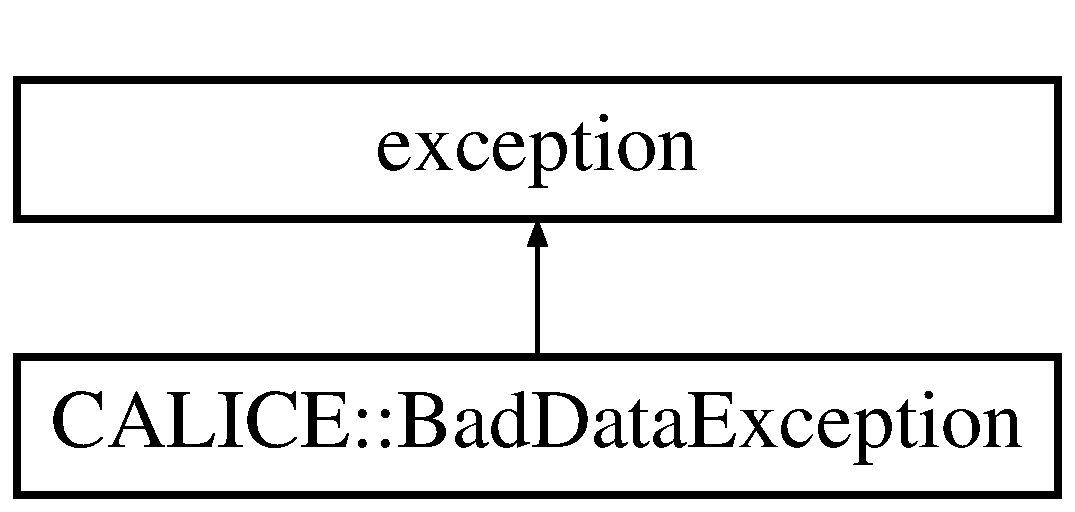
\includegraphics[height=2.000000cm]{classCALICE_1_1BadDataException}
\end{center}
\end{figure}
\subsection*{Public Member Functions}
\begin{DoxyCompactItemize}
\item 
{\bfseries Bad\-Data\-Exception} (std\-::string text)  throw ()\label{classCALICE_1_1BadDataException_a765bc2673e0be6a8371b058b3fbe4a4e}

\item 
const char $\ast$ {\bfseries what} () const   throw ()\label{classCALICE_1_1BadDataException_aee526e91ff2f998e8420baac9c070546}

\end{DoxyCompactItemize}
\subsection*{Protected Attributes}
\begin{DoxyCompactItemize}
\item 
std\-::string {\bfseries \-\_\-message}\label{classCALICE_1_1BadDataException_aca1e20b6d7f88c0cd5dbacb38b462386}

\end{DoxyCompactItemize}


\subsection{Detailed Description}
exception to be thrown when data leads to a conflict 



Definition at line 37 of file Calice\-Exception.\-hh.



The documentation for this class was generated from the following file\-:\begin{DoxyCompactItemize}
\item 
Calice\-Exception.\-hh\end{DoxyCompactItemize}

\section{C\-A\-L\-I\-C\-E\-:\-:Beam\-Meta\-Data Class Reference}
\label{classCALICE_1_1BeamMetaData}\index{C\-A\-L\-I\-C\-E\-::\-Beam\-Meta\-Data@{C\-A\-L\-I\-C\-E\-::\-Beam\-Meta\-Data}}
Inheritance diagram for C\-A\-L\-I\-C\-E\-:\-:Beam\-Meta\-Data\-:\begin{figure}[H]
\begin{center}
\leavevmode
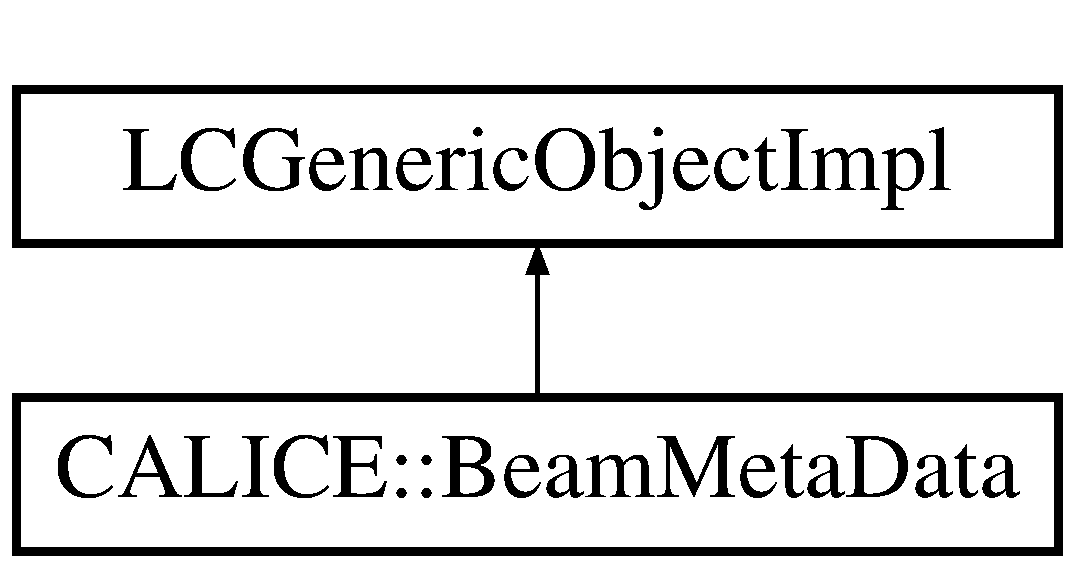
\includegraphics[height=2.000000cm]{classCALICE_1_1BeamMetaData}
\end{center}
\end{figure}
\subsection*{Public Member Functions}
\begin{DoxyCompactItemize}
\item 
{\bfseries Beam\-Meta\-Data} (const int \&pdg\-Code, const float \&energy)\label{classCALICE_1_1BeamMetaData_ac22d51f9f4ac31beae53b0ace01fafd0}

\item 
{\bfseries Beam\-Meta\-Data} (L\-C\-Generic\-Object $\ast$obj)\label{classCALICE_1_1BeamMetaData_ac0f69e98cee9d162ba93f5620d1e05e6}

\item 
const int {\bfseries get\-Pdg\-Code} () const \label{classCALICE_1_1BeamMetaData_a71fc431fc1c25ca0d310a8a3980c4656}

\item 
const float {\bfseries get\-Energy} () const \label{classCALICE_1_1BeamMetaData_a7b6054aeeeee3ad83f468466f7835c7e}

\item 
void {\bfseries set\-Pdg\-Code} (const int \&pdg\-Code)\label{classCALICE_1_1BeamMetaData_a73a59e54ded8ad2f88f1ce894d56cef2}

\item 
void {\bfseries set\-Energy} (const float \&energy)\label{classCALICE_1_1BeamMetaData_a72048e8487e9c9711cc0edf98367a7fd}

\end{DoxyCompactItemize}
\subsection*{Protected Types}
\begin{DoxyCompactItemize}
\item 
enum {\bfseries Ints} \{ {\bfseries k\-Pdg\-Code}, 
{\bfseries k\-N\-Ints}
 \}
\item 
enum {\bfseries Floats} \{ {\bfseries k\-Energy}, 
{\bfseries k\-N\-Floats}
 \}
\item 
enum {\bfseries Doubless} \{ {\bfseries k\-N\-Doubles}
 \}
\end{DoxyCompactItemize}
\subsection*{Protected Member Functions}
\begin{DoxyCompactItemize}
\item 
void {\bfseries set} (L\-C\-Generic\-Object $\ast$obj)\label{classCALICE_1_1BeamMetaData_a70518a4d2e7e10c1e476dccd9cf82b4f}

\end{DoxyCompactItemize}
\subsection*{Private Attributes}
\begin{DoxyCompactItemize}
\item 
int {\bfseries \-\_\-pdg\-Type}\label{classCALICE_1_1BeamMetaData_a1e3ee81446b50e78dbc12b16b8aac6ee}

\item 
float {\bfseries \-\_\-energy}\label{classCALICE_1_1BeamMetaData_ad92f231b44646ed3931c6fbcb02f65aa}

\end{DoxyCompactItemize}


\subsection{Detailed Description}


Definition at line 9 of file Beam\-Meta\-Data.\-hh.



The documentation for this class was generated from the following files\-:\begin{DoxyCompactItemize}
\item 
Beam\-Meta\-Data.\-hh\item 
Beam\-Meta\-Data.\-cc\end{DoxyCompactItemize}

\section{C\-A\-L\-I\-C\-E\-:\-:Beam\-Momentum Class Reference}
\label{classCALICE_1_1BeamMomentum}\index{C\-A\-L\-I\-C\-E\-::\-Beam\-Momentum@{C\-A\-L\-I\-C\-E\-::\-Beam\-Momentum}}


Class to claculate the beam momentum and momentum spread from beamline slow readout data.  




{\ttfamily \#include $<$Beam\-Momentum.\-hh$>$}

\subsection*{Public Member Functions}
\begin{DoxyCompactItemize}
\item 
{\bf Beam\-Momentum} (const {\bf C\-A\-L\-I\-C\-E\-::\-Bml\-Slow\-Run\-Data\-Block} \&cern\-Beam\-Data)
\begin{DoxyCompactList}\small\item\em Construcor using C\-E\-R\-N data as input. \end{DoxyCompactList}\item 
double {\bf get\-Momentum} () const 
\item 
double {\bf get\-Secondary\-Momentum} () const 
\item 
double {\bf get\-Tertiary\-Momentum} () const 
\item 
double {\bf get\-Relative\-Spread} () const 
\item 
double {\bf get\-Momentum\-Spread} () const 
\item 
double {\bf get\-Limited\-Relative\-Spread} () const 
\begin{DoxyCompactList}\small\item\em this returns a limited spread for secondary beams, please read the class description \end{DoxyCompactList}\item 
double {\bf get\-Limited\-Momentum\-Spread} () const 
\begin{DoxyCompactList}\small\item\em this returns a limited spread for secondary beams, please read the class description \end{DoxyCompactList}\item 
const std\-::string {\bf get\-Warnings} () const 
\end{DoxyCompactItemize}
\subsection*{Private Attributes}
\begin{DoxyCompactItemize}
\item 
double {\bfseries \-\_\-momentum}\label{classCALICE_1_1BeamMomentum_ab5a1406c4ee908d6191e579d5269ad82}

\item 
double {\bfseries \-\_\-secondary\-Momentum}\label{classCALICE_1_1BeamMomentum_aedd80f5b4994fc065d015eecf3aca9d9}

\item 
double {\bfseries \-\_\-tertiary\-Momentum}\label{classCALICE_1_1BeamMomentum_af1bae196b4deedf5338525233e040b46}

\item 
double {\bfseries \-\_\-relative\-Spread}\label{classCALICE_1_1BeamMomentum_a2423b7ace1c4d2583a1d2b41987078b9}

\item 
double {\bfseries \-\_\-limited\-Relative\-Spread}\label{classCALICE_1_1BeamMomentum_a2769dd2776a49367360f8afebb4bef6d}

\item 
std\-::stringstream {\bfseries \-\_\-warning\-Text}\label{classCALICE_1_1BeamMomentum_ae15697c4beb991a607364bef48a813fa}

\end{DoxyCompactItemize}


\subsection{Detailed Description}
Class to claculate the beam momentum and momentum spread from beamline slow readout data. 

The beam momentum is linearly approximated from the magnet currents. A Gaussian distribution of the beam momentum spread is assumed.

\begin{DoxyParagraph}{C\-E\-R\-N}
The calculations are based on the informations found in the {\bfseries \char`\"{}\-Short Introduction to the use of the H6 beam\char`\"{}}, Version 3.\-0, 2 May 2000.
\end{DoxyParagraph}
\begin{DoxyParagraph}{}
There are no references found for the current to momentum translation for most of the magnets. The {\bfseries Introduction} tells only that B(end)5 should be at 566.\-4\-A for 120 Ge\-V. Therefore, the slope was fitted on a few runs. For B5 the fit gives the same result as the {\bfseries Introduction}.
\end{DoxyParagraph}
\begin{DoxyParagraph}{}
The {\bfseries full} {\bfseries width} beam momentum spread is calculated by the formula \[ \frac{\Delta p}{p} = \frac{\sqrt{C_{3}^2+C_{8}^2}}{19.4} [\%] \] where $ C_{i} $ is the {\bfseries full} {\bfseries width} opening of collimator $i$. This is valid for tertiary beams.
\end{DoxyParagraph}
\begin{DoxyParagraph}{}
For secondary beams this might lead to an overestimation of the beam spread, as $C_{8}$ might be further open than the beam size. The {\bfseries Introduction} suggest to use $ C_{8} = $ 4mm as upper limit for high energy secondary beams. This class provides limited and unlimited results, as it is not clear to the author when a beam can be considered \char`\"{}high energy\char`\"{} and the destinction between secondary and tertiary beam by target position fails in 2007. The beam is considered secondary, if the beam momentum in the secondary and the tertiary section differ for less than 10 \%. In this case, a warning message is issued.
\end{DoxyParagraph}
\begin{DoxyParagraph}{}
The Gaussian width is derived by \[ \sigma = \frac{\Delta p}{2\sqrt{2\ln{2}}} \approx \frac{\Delta p}{2.35482} \]
\end{DoxyParagraph}
\begin{DoxyAttention}{Attention}
The implementation supports only C\-E\-R\-N so far
\end{DoxyAttention}
\begin{DoxyRefDesc}{Todo}
\item[{\bf Todo}]implement a constructor for F\-N\-A\-L slow readout data\end{DoxyRefDesc}


\begin{DoxyAuthor}{Author}
{\tt Benjamin.\-Lutz@desy.\-de} 
\end{DoxyAuthor}
\begin{DoxyVersion}{Version}
1.\-0 
\end{DoxyVersion}
\begin{DoxyDate}{Date}
October 2008 
\end{DoxyDate}


Definition at line 48 of file Beam\-Momentum.\-hh.



\subsection{Constructor \& Destructor Documentation}
\index{C\-A\-L\-I\-C\-E\-::\-Beam\-Momentum@{C\-A\-L\-I\-C\-E\-::\-Beam\-Momentum}!Beam\-Momentum@{Beam\-Momentum}}
\index{Beam\-Momentum@{Beam\-Momentum}!CALICE::BeamMomentum@{C\-A\-L\-I\-C\-E\-::\-Beam\-Momentum}}
\subsubsection[{Beam\-Momentum}]{\setlength{\rightskip}{0pt plus 5cm}C\-A\-L\-I\-C\-E\-::\-Beam\-Momentum\-::\-Beam\-Momentum (
\begin{DoxyParamCaption}
\item[{const {\bf C\-A\-L\-I\-C\-E\-::\-Bml\-Slow\-Run\-Data\-Block} \&}]{cern\-Beam\-Data}
\end{DoxyParamCaption}
)}\label{classCALICE_1_1BeamMomentum_aa27dc27234e98e1ad8115049f1b4c202}


Construcor using C\-E\-R\-N data as input. 


\begin{DoxyExceptions}{Exceptions}
{\em \doxyref{Beam\-Momentum\-Exception}{p.}{classCALICE_1_1BeamMomentumException}} & when number of magnet currents or collimators does not corresond to the C\-E\-R\-N beamline \\
\hline
\end{DoxyExceptions}


Definition at line 10 of file Beam\-Momentum.\-cc.



References C\-A\-L\-I\-C\-E\-::\-Bml\-Slow\-Run\-Data\-Block\-::get\-Bend\-Currents(), and C\-A\-L\-I\-C\-E\-::\-Bml\-Slow\-Run\-Data\-Block\-::get\-Collimator\-Positions().



\subsection{Member Function Documentation}
\index{C\-A\-L\-I\-C\-E\-::\-Beam\-Momentum@{C\-A\-L\-I\-C\-E\-::\-Beam\-Momentum}!get\-Limited\-Momentum\-Spread@{get\-Limited\-Momentum\-Spread}}
\index{get\-Limited\-Momentum\-Spread@{get\-Limited\-Momentum\-Spread}!CALICE::BeamMomentum@{C\-A\-L\-I\-C\-E\-::\-Beam\-Momentum}}
\subsubsection[{get\-Limited\-Momentum\-Spread}]{\setlength{\rightskip}{0pt plus 5cm}double C\-A\-L\-I\-C\-E\-::\-Beam\-Momentum\-::get\-Limited\-Momentum\-Spread (
\begin{DoxyParamCaption}
{}
\end{DoxyParamCaption}
) const}\label{classCALICE_1_1BeamMomentum_a124b5dd4915b4d0b2d9f0c96985565ae}


this returns a limited spread for secondary beams, please read the class description 

\begin{DoxyReturn}{Returns}
beam momentum spread in Ge\-V 
\end{DoxyReturn}


Definition at line 141 of file Beam\-Momentum.\-cc.

\index{C\-A\-L\-I\-C\-E\-::\-Beam\-Momentum@{C\-A\-L\-I\-C\-E\-::\-Beam\-Momentum}!get\-Limited\-Relative\-Spread@{get\-Limited\-Relative\-Spread}}
\index{get\-Limited\-Relative\-Spread@{get\-Limited\-Relative\-Spread}!CALICE::BeamMomentum@{C\-A\-L\-I\-C\-E\-::\-Beam\-Momentum}}
\subsubsection[{get\-Limited\-Relative\-Spread}]{\setlength{\rightskip}{0pt plus 5cm}double C\-A\-L\-I\-C\-E\-::\-Beam\-Momentum\-::get\-Limited\-Relative\-Spread (
\begin{DoxyParamCaption}
{}
\end{DoxyParamCaption}
) const}\label{classCALICE_1_1BeamMomentum_ab7883995158ee69aa47b7ed808d0b51a}


this returns a limited spread for secondary beams, please read the class description 

\begin{DoxyReturn}{Returns}
relative beam momentum spread 
\end{DoxyReturn}


Definition at line 137 of file Beam\-Momentum.\-cc.

\index{C\-A\-L\-I\-C\-E\-::\-Beam\-Momentum@{C\-A\-L\-I\-C\-E\-::\-Beam\-Momentum}!get\-Momentum@{get\-Momentum}}
\index{get\-Momentum@{get\-Momentum}!CALICE::BeamMomentum@{C\-A\-L\-I\-C\-E\-::\-Beam\-Momentum}}
\subsubsection[{get\-Momentum}]{\setlength{\rightskip}{0pt plus 5cm}double C\-A\-L\-I\-C\-E\-::\-Beam\-Momentum\-::get\-Momentum (
\begin{DoxyParamCaption}
{}
\end{DoxyParamCaption}
) const}\label{classCALICE_1_1BeamMomentum_a98b2a24c31c0afb62b280caaae5d69cc}
\begin{DoxyReturn}{Returns}
the beam momentum in Ge\-V 
\end{DoxyReturn}


Definition at line 117 of file Beam\-Momentum.\-cc.

\index{C\-A\-L\-I\-C\-E\-::\-Beam\-Momentum@{C\-A\-L\-I\-C\-E\-::\-Beam\-Momentum}!get\-Momentum\-Spread@{get\-Momentum\-Spread}}
\index{get\-Momentum\-Spread@{get\-Momentum\-Spread}!CALICE::BeamMomentum@{C\-A\-L\-I\-C\-E\-::\-Beam\-Momentum}}
\subsubsection[{get\-Momentum\-Spread}]{\setlength{\rightskip}{0pt plus 5cm}double C\-A\-L\-I\-C\-E\-::\-Beam\-Momentum\-::get\-Momentum\-Spread (
\begin{DoxyParamCaption}
{}
\end{DoxyParamCaption}
) const}\label{classCALICE_1_1BeamMomentum_a1136a4941aca0feab6ac7a748d456c26}
\begin{DoxyReturn}{Returns}
beam momentum spread in Ge\-V 
\end{DoxyReturn}


Definition at line 133 of file Beam\-Momentum.\-cc.

\index{C\-A\-L\-I\-C\-E\-::\-Beam\-Momentum@{C\-A\-L\-I\-C\-E\-::\-Beam\-Momentum}!get\-Relative\-Spread@{get\-Relative\-Spread}}
\index{get\-Relative\-Spread@{get\-Relative\-Spread}!CALICE::BeamMomentum@{C\-A\-L\-I\-C\-E\-::\-Beam\-Momentum}}
\subsubsection[{get\-Relative\-Spread}]{\setlength{\rightskip}{0pt plus 5cm}double C\-A\-L\-I\-C\-E\-::\-Beam\-Momentum\-::get\-Relative\-Spread (
\begin{DoxyParamCaption}
{}
\end{DoxyParamCaption}
) const}\label{classCALICE_1_1BeamMomentum_acea65b8dc19544ceb52b31d1b69ff6d7}
\begin{DoxyReturn}{Returns}
relative beam momentum spread 
\end{DoxyReturn}


Definition at line 129 of file Beam\-Momentum.\-cc.

\index{C\-A\-L\-I\-C\-E\-::\-Beam\-Momentum@{C\-A\-L\-I\-C\-E\-::\-Beam\-Momentum}!get\-Secondary\-Momentum@{get\-Secondary\-Momentum}}
\index{get\-Secondary\-Momentum@{get\-Secondary\-Momentum}!CALICE::BeamMomentum@{C\-A\-L\-I\-C\-E\-::\-Beam\-Momentum}}
\subsubsection[{get\-Secondary\-Momentum}]{\setlength{\rightskip}{0pt plus 5cm}double C\-A\-L\-I\-C\-E\-::\-Beam\-Momentum\-::get\-Secondary\-Momentum (
\begin{DoxyParamCaption}
{}
\end{DoxyParamCaption}
) const}\label{classCALICE_1_1BeamMomentum_afad1bc1ae90b11d91d9f615584d7ac9d}
\begin{DoxyReturn}{Returns}
the beam momentum before the secondary target 
\end{DoxyReturn}


Definition at line 121 of file Beam\-Momentum.\-cc.

\index{C\-A\-L\-I\-C\-E\-::\-Beam\-Momentum@{C\-A\-L\-I\-C\-E\-::\-Beam\-Momentum}!get\-Tertiary\-Momentum@{get\-Tertiary\-Momentum}}
\index{get\-Tertiary\-Momentum@{get\-Tertiary\-Momentum}!CALICE::BeamMomentum@{C\-A\-L\-I\-C\-E\-::\-Beam\-Momentum}}
\subsubsection[{get\-Tertiary\-Momentum}]{\setlength{\rightskip}{0pt plus 5cm}double C\-A\-L\-I\-C\-E\-::\-Beam\-Momentum\-::get\-Tertiary\-Momentum (
\begin{DoxyParamCaption}
{}
\end{DoxyParamCaption}
) const}\label{classCALICE_1_1BeamMomentum_a5f70de92c980e0abc7e42b076d6d013d}
\begin{DoxyReturn}{Returns}
the beam momentum after the secondary target 
\end{DoxyReturn}


Definition at line 125 of file Beam\-Momentum.\-cc.

\index{C\-A\-L\-I\-C\-E\-::\-Beam\-Momentum@{C\-A\-L\-I\-C\-E\-::\-Beam\-Momentum}!get\-Warnings@{get\-Warnings}}
\index{get\-Warnings@{get\-Warnings}!CALICE::BeamMomentum@{C\-A\-L\-I\-C\-E\-::\-Beam\-Momentum}}
\subsubsection[{get\-Warnings}]{\setlength{\rightskip}{0pt plus 5cm}const std\-::string C\-A\-L\-I\-C\-E\-::\-Beam\-Momentum\-::get\-Warnings (
\begin{DoxyParamCaption}
{}
\end{DoxyParamCaption}
) const}\label{classCALICE_1_1BeamMomentum_a1b09ead51b46163bb14e5f8802bf7714}
\begin{DoxyReturn}{Returns}
warnings that occured during interpretation of beam settings 
\end{DoxyReturn}


Definition at line 145 of file Beam\-Momentum.\-cc.



The documentation for this class was generated from the following files\-:\begin{DoxyCompactItemize}
\item 
Beam\-Momentum.\-hh\item 
Beam\-Momentum.\-cc\end{DoxyCompactItemize}

\section{C\-A\-L\-I\-C\-E\-:\-:Beam\-Momentum\-Exception Class Reference}
\label{classCALICE_1_1BeamMomentumException}\index{C\-A\-L\-I\-C\-E\-::\-Beam\-Momentum\-Exception@{C\-A\-L\-I\-C\-E\-::\-Beam\-Momentum\-Exception}}


excpetion during beam momentum calculation  




{\ttfamily \#include $<$Beam\-Momentum.\-hh$>$}

\subsection*{Public Member Functions}
\begin{DoxyCompactItemize}
\item 
{\bf Beam\-Momentum\-Exception} (std\-::string {\bf what})
\item 
const std\-::string {\bf what} () const \label{classCALICE_1_1BeamMomentumException_abf96d139d64de8fd11114234cac573f8}

\begin{DoxyCompactList}\small\item\em tell what caused the exception \end{DoxyCompactList}\end{DoxyCompactItemize}
\subsection*{Protected Attributes}
\begin{DoxyCompactItemize}
\item 
std\-::string {\bfseries \-\_\-type}\label{classCALICE_1_1BeamMomentumException_a6e2c3f65164d99f3e01a2eb02d88701d}

\item 
std\-::string {\bfseries \-\_\-what}\label{classCALICE_1_1BeamMomentumException_a8cbcb9dc73807afc3db99a463baa0933}

\end{DoxyCompactItemize}


\subsection{Detailed Description}
excpetion during beam momentum calculation 

Definition at line 112 of file Beam\-Momentum.\-hh.



\subsection{Constructor \& Destructor Documentation}
\index{C\-A\-L\-I\-C\-E\-::\-Beam\-Momentum\-Exception@{C\-A\-L\-I\-C\-E\-::\-Beam\-Momentum\-Exception}!Beam\-Momentum\-Exception@{Beam\-Momentum\-Exception}}
\index{Beam\-Momentum\-Exception@{Beam\-Momentum\-Exception}!CALICE::BeamMomentumException@{C\-A\-L\-I\-C\-E\-::\-Beam\-Momentum\-Exception}}
\subsubsection[{Beam\-Momentum\-Exception}]{\setlength{\rightskip}{0pt plus 5cm}C\-A\-L\-I\-C\-E\-::\-Beam\-Momentum\-Exception\-::\-Beam\-Momentum\-Exception (
\begin{DoxyParamCaption}
\item[{std\-::string}]{what}
\end{DoxyParamCaption}
)\hspace{0.3cm}{\ttfamily [inline]}}\label{classCALICE_1_1BeamMomentumException_abbab9053af44936a75964dfafd1824ed}

\begin{DoxyParams}{Parameters}
{\em what} & Reason of the exception. \\
\hline
\end{DoxyParams}


Definition at line 117 of file Beam\-Momentum.\-hh.



The documentation for this class was generated from the following file\-:\begin{DoxyCompactItemize}
\item 
Beam\-Momentum.\-hh\end{DoxyCompactItemize}

\section{C\-A\-L\-I\-C\-E\-:\-:Beam\-Parameter Class Reference}
\label{classCALICE_1_1BeamParameter}\index{C\-A\-L\-I\-C\-E\-::\-Beam\-Parameter@{C\-A\-L\-I\-C\-E\-::\-Beam\-Parameter}}


Define the experimental setup\-: beam energy, position, angle and detector position, angle.  




{\ttfamily \#include $<$Beam\-Parameter.\-hh$>$}

Inheritance diagram for C\-A\-L\-I\-C\-E\-:\-:Beam\-Parameter\-:\begin{figure}[H]
\begin{center}
\leavevmode
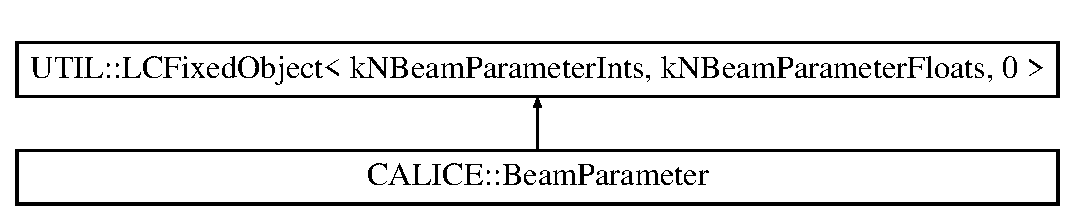
\includegraphics[height=2.000000cm]{classCALICE_1_1BeamParameter}
\end{center}
\end{figure}
\subsection*{Public Types}
\begin{DoxyCompactItemize}
\item 
enum {\bfseries E\-Beam\-Type} \{ \\*
{\bfseries k\-Electron\-Beam}, 
{\bfseries k\-Muon\-Beam}, 
{\bfseries k\-Pion\-Beam}, 
{\bfseries k\-Proton\-Beam}, 
\\*
{\bfseries k\-Cosmics}, 
{\bfseries k\-Unknown}, 
{\bfseries k\-Mixed}, 
{\bfseries k\-Pion\-Electron\-Beam}, 
\\*
{\bfseries k\-Pion\-Proton\-Beam}, 
{\bfseries k\-Calibration\-Pulse}, 
{\bfseries k\-Noise}, 
{\bfseries k\-N\-Beam\-Types}
 \}
\end{DoxyCompactItemize}
\subsection*{Public Member Functions}
\begin{DoxyCompactItemize}
\item 
{\bf Beam\-Parameter} (L\-C\-Object $\ast$obj)\label{classCALICE_1_1BeamParameter_ac34c61a0ff07d533fa175cdea702b8fe}

\begin{DoxyCompactList}\small\item\em 'Copy constructor' needed to interpret L\-C\-Collection read from file/database. \end{DoxyCompactList}\item 
{\bf Beam\-Parameter} \& {\bf set\-Beam\-Type} (E\-Beam\-Type beam\-\_\-type)\label{classCALICE_1_1BeamParameter_a91a84f9a224e2b2840fe1aa1e8bab3ec}

\begin{DoxyCompactList}\small\item\em Set the particle type. \end{DoxyCompactList}\item 
E\-Beam\-Type {\bf get\-Beam\-Type} () const \label{classCALICE_1_1BeamParameter_af8ed22618fedce8bd2840c658ed79ee0}

\begin{DoxyCompactList}\small\item\em Get the particle type. \end{DoxyCompactList}\item 
const char $\ast$ {\bf get\-Beam\-Type\-Name} () const \label{classCALICE_1_1BeamParameter_ae2ffbfa7c92c6057139bd4a8b5b1fe8c}

\begin{DoxyCompactList}\small\item\em Return the beam type name. \end{DoxyCompactList}\item 
{\bf Beam\-Parameter} \& {\bf set\-Peak\-Energy} (float peak\-\_\-energy)\label{classCALICE_1_1BeamParameter_a9868e1e09ffff9f945faa8427f5f5ef5}

\begin{DoxyCompactList}\small\item\em Set the maximum of the beam energy distribution. \end{DoxyCompactList}\item 
float {\bf get\-Peak\-Energy} () const \label{classCALICE_1_1BeamParameter_aecdce6fd9dc5911ea36a41a73ed04c72}

\begin{DoxyCompactList}\small\item\em Get the maximum of the beam energy distribution. \end{DoxyCompactList}\item 
{\bf Beam\-Parameter} \& {\bf set\-Beam\-Angle\-Z\-X} (float beam\-\_\-angle\-\_\-zx)\label{classCALICE_1_1BeamParameter_ac1987bb9375229234b7bcd90c401f7bf}

\begin{DoxyCompactList}\small\item\em Set the angle between the beam and the z-\/axis in thr Z\-X plane. \end{DoxyCompactList}\item 
float {\bf get\-Beam\-Angle\-Z\-X} () const \label{classCALICE_1_1BeamParameter_a0521b37942f8761e317b7780450c746d}

\begin{DoxyCompactList}\small\item\em Get Set the angle between the beam and the z-\/axis in thr Z\-X plane. \end{DoxyCompactList}\item 
{\bf Beam\-Parameter} \& {\bf set\-Beam\-Angle\-Z\-Y} (float beam\-\_\-angle\-\_\-zy)\label{classCALICE_1_1BeamParameter_a861b31336d44f2084a325c3968eaa9bb}

\begin{DoxyCompactList}\small\item\em Set the angle between the beam and the z-\/axis in thr Z\-Y plane. \end{DoxyCompactList}\item 
float {\bf get\-Beam\-Angle\-Z\-Y} () const \label{classCALICE_1_1BeamParameter_ac32fcba57ab64d4fcfd704bfc2ef627e}

\begin{DoxyCompactList}\small\item\em Get the angle between the beam and the z-\/axis in thr Z\-Y plane. \end{DoxyCompactList}\item 
{\bf Beam\-Parameter} \& {\bf set\-Beam\-Impact\-Position} (float beam\-\_\-impact\-\_\-x0, float beam\-\_\-impact\-\_\-y0)\label{classCALICE_1_1BeamParameter_a0e5034d96cf4bad36b3e8757c5b57700}

\begin{DoxyCompactList}\small\item\em Set the mean impact position of the beam on the detector in the X\-Y-\/plane (convenience method). \end{DoxyCompactList}\item 
{\bf Beam\-Parameter} \& {\bf set\-Beam\-Impact\-Position} (float $\ast$beam\-\_\-impact\-\_\-position\-\_\-tupel)\label{classCALICE_1_1BeamParameter_ac9bbf019b9a990aa64762c4f8383a235}

\begin{DoxyCompactList}\small\item\em Set the mean impact position of the beam on the detector in the X\-Y-\/plane (convenience method). \end{DoxyCompactList}\item 
{\bf Beam\-Parameter} \& {\bf set\-Beam\-Impact\-Position\-X0} (float beam\-\_\-impact\-\_\-x0)\label{classCALICE_1_1BeamParameter_a1ec83a4202220110e1f149dae22e6a60}

\begin{DoxyCompactList}\small\item\em Set the mean impact position of the beam on the detector in the X\-Y-\/plane. \end{DoxyCompactList}\item 
float {\bf get\-Beam\-Impact\-Position\-X0} () const \label{classCALICE_1_1BeamParameter_a3f9caa58f8a6b1dcc3b2a2effc056221}

\begin{DoxyCompactList}\small\item\em Get the mean impact position of the beam on the detector in the X\-Y-\/plane. \end{DoxyCompactList}\item 
{\bf Beam\-Parameter} \& {\bf set\-Beam\-Impact\-Position\-Y0} (float beam\-\_\-impact\-\_\-y0)\label{classCALICE_1_1BeamParameter_a21742c669e7e1319b384a56b9dad9d25}

\begin{DoxyCompactList}\small\item\em Set the mean impact position of the beam on the detector in the X\-Y-\/plane. \end{DoxyCompactList}\item 
float {\bf get\-Beam\-Impact\-Position\-Y0} () const \label{classCALICE_1_1BeamParameter_a467abe590bc12553cfc297744aeece5c}

\begin{DoxyCompactList}\small\item\em Get the y-\/coordinate of the mean impact position of the beam on the detector in the X\-Y-\/plane. \end{DoxyCompactList}\item 
void {\bf print} (std\-::ostream \&os)\label{classCALICE_1_1BeamParameter_a17b85ed30ff0f0d9eb1b2d1935ef9bed}

\begin{DoxyCompactList}\small\item\em Print all members (for debugging) \end{DoxyCompactList}\item 
const std\-::string {\bf get\-Type\-Name} () const \label{classCALICE_1_1BeamParameter_aa5a1c4f371d71c513584a106f69ee940}

\begin{DoxyCompactList}\small\item\em Return the type of the class. \end{DoxyCompactList}\item 
const std\-::string {\bf get\-Data\-Description} () const \label{classCALICE_1_1BeamParameter_adf804091f7b3991b2dbec8bc9b5db5fb}

\begin{DoxyCompactList}\small\item\em Return a brief description of the data members. \end{DoxyCompactList}\end{DoxyCompactItemize}
\subsection*{Static Public Member Functions}
\begin{DoxyCompactItemize}
\item 
static const char $\ast$ {\bf get\-Beam\-Type\-Name} (unsigned int beam\-\_\-type\-\_\-i)\label{classCALICE_1_1BeamParameter_add13ac5aa7c9fab9a5572f6673ff8dc6}

\begin{DoxyCompactList}\small\item\em Return the beam type name for a given type id. \end{DoxyCompactList}\end{DoxyCompactItemize}
\subsection*{Static Public Attributes}
\begin{DoxyCompactItemize}
\item 
static const char $\ast$ {\bfseries \-\_\-\-\_\-beam\-Type\-Names} [C\-A\-L\-I\-C\-E\-::\-Beam\-Parameter\-::k\-N\-Beam\-Types+1]
\end{DoxyCompactItemize}


\subsection{Detailed Description}
Define the experimental setup\-: beam energy, position, angle and detector position, angle. 

The experimental setup should be written into the conditions database at least twice\-: 
\begin{DoxyItemize}
\item the nominal values with the tag N\-O\-M\-I\-N\-A\-L 
\item the measured values 
\end{DoxyItemize}\begin{DoxyRefDesc}{Todo}
\item[{\bf Todo}]\{Should this class be split into two? One for the beam and one for the detector parameters? Should the nominal and measured values be stored in separate folders?\} \end{DoxyRefDesc}


Definition at line 37 of file Beam\-Parameter.\-hh.



\subsection{Field Documentation}
\index{C\-A\-L\-I\-C\-E\-::\-Beam\-Parameter@{C\-A\-L\-I\-C\-E\-::\-Beam\-Parameter}!\-\_\-\-\_\-beam\-Type\-Names@{\-\_\-\-\_\-beam\-Type\-Names}}
\index{\-\_\-\-\_\-beam\-Type\-Names@{\-\_\-\-\_\-beam\-Type\-Names}!CALICE::BeamParameter@{C\-A\-L\-I\-C\-E\-::\-Beam\-Parameter}}
\subsubsection[{\-\_\-\-\_\-beam\-Type\-Names}]{\setlength{\rightskip}{0pt plus 5cm}const char $\ast$ C\-A\-L\-I\-C\-E\-::\-Beam\-Parameter\-::\-\_\-\-\_\-beam\-Type\-Names\hspace{0.3cm}{\ttfamily [static]}}\label{classCALICE_1_1BeamParameter_a5bab90e1ec133f8427213561be2fc669}
{\bfseries Initial value\-:}
\begin{DoxyCode}
=\{
    \textcolor{stringliteral}{"electron"},
    \textcolor{stringliteral}{"muon"},
    \textcolor{stringliteral}{"pion"},
    \textcolor{stringliteral}{"proton"},
    \textcolor{stringliteral}{"cosmics"},
    \textcolor{stringliteral}{"unknown"},
    \textcolor{stringliteral}{"mixed"}, 
    \textcolor{stringliteral}{"pion+electron"},
    \textcolor{stringliteral}{"pion+proton"},
    \textcolor{stringliteral}{"calibration"},
    \textcolor{stringliteral}{"noise"},
    \textcolor{stringliteral}{"(out of range)"},
  \}
\end{DoxyCode}


Definition at line 184 of file Beam\-Parameter.\-hh.



The documentation for this class was generated from the following files\-:\begin{DoxyCompactItemize}
\item 
Beam\-Parameter.\-hh\item 
Beam\-Parameter.\-cc\end{DoxyCompactItemize}

\section{C\-A\-L\-I\-C\-E\-:\-:Beam\-Parameter\-Exception Class Reference}
\label{classCALICE_1_1BeamParameterException}\index{C\-A\-L\-I\-C\-E\-::\-Beam\-Parameter\-Exception@{C\-A\-L\-I\-C\-E\-::\-Beam\-Parameter\-Exception}}


This class handles beam parameters which have been written by hand into the database.  




{\ttfamily \#include $<$Beam\-Parameter\-Exception.\-hh$>$}

Inheritance diagram for C\-A\-L\-I\-C\-E\-:\-:Beam\-Parameter\-Exception\-:\begin{figure}[H]
\begin{center}
\leavevmode
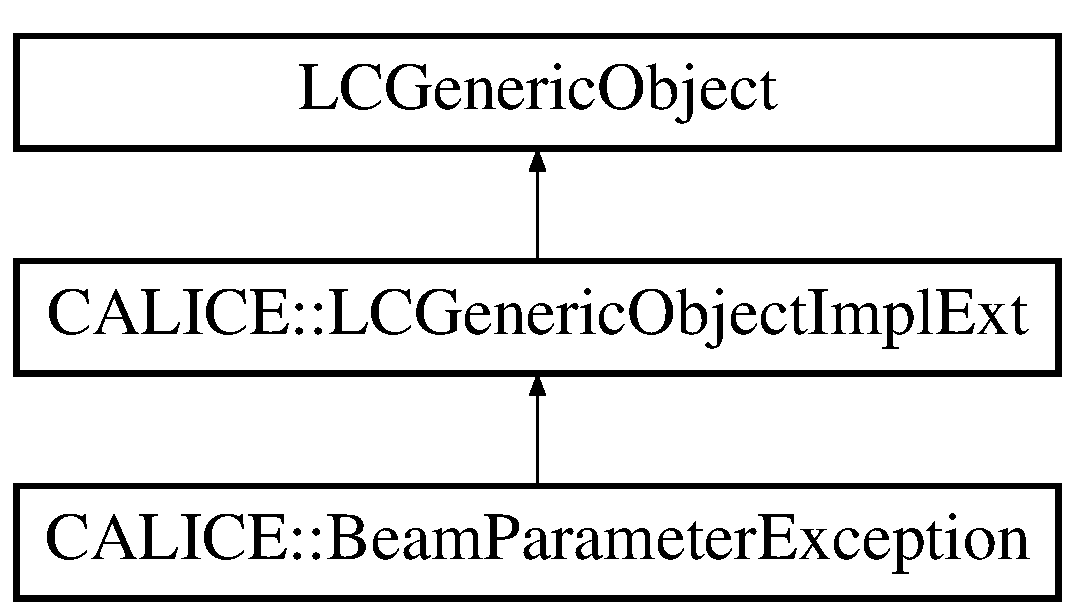
\includegraphics[height=3.000000cm]{classCALICE_1_1BeamParameterException}
\end{center}
\end{figure}
\subsection*{Public Member Functions}
\begin{DoxyCompactItemize}
\item 
{\bf Beam\-Parameter\-Exception} (L\-C\-Object $\ast${\bf obj})\label{classCALICE_1_1BeamParameterException_a8ae0f2f91f0d1a8d757cfafc6f9040b7}

\begin{DoxyCompactList}\small\item\em 'Copy constructor' needed to interpret L\-C\-Collection read from file/database. \end{DoxyCompactList}\item 
{\bf Beam\-Parameter\-Exception} \& {\bf set\-Beam\-Energy} (unsigned int energy)
\begin{DoxyCompactList}\small\item\em Set the particle type. \end{DoxyCompactList}\item 
unsigned int {\bf get\-Beam\-Energy} () const \label{classCALICE_1_1BeamParameterException_a207e7eed23b2eb26389e20af3a4a4d6d}

\begin{DoxyCompactList}\small\item\em Get the maximum of the beam energy distribution. \end{DoxyCompactList}\item 
void {\bf print} (std\-::ostream \&os)\label{classCALICE_1_1BeamParameterException_ad198507745bc2607d95f62d671f3ae56}

\begin{DoxyCompactList}\small\item\em Print all members (for debugging) \end{DoxyCompactList}\item 
const std\-::string {\bf get\-Type\-Name} () const \label{classCALICE_1_1BeamParameterException_a03e95b25675a8b394ae4e75781c52a46}

\begin{DoxyCompactList}\small\item\em Return the type of the class. \end{DoxyCompactList}\item 
const std\-::string {\bf get\-Data\-Description} () const \label{classCALICE_1_1BeamParameterException_ad3e64e3f1fa0fabe6689639f0a2f6c68}

\begin{DoxyCompactList}\small\item\em Return a brief description of the data members. \end{DoxyCompactList}\end{DoxyCompactItemize}
\subsection*{Additional Inherited Members}


\subsection{Detailed Description}
This class handles beam parameters which have been written by hand into the database. 

It is to be used if beam parameters are either not available at all or if the analysis of the r/o has revealed some odds. This class might evolve with time, for the time being it constains only the beam energy. \begin{DoxyAuthor}{Author}
R. P�schl L\-A\-L 
\end{DoxyAuthor}
\begin{DoxyDate}{Date}
Oct 2007 
\end{DoxyDate}


Definition at line 28 of file Beam\-Parameter\-Exception.\-hh.



\subsection{Member Function Documentation}
\index{C\-A\-L\-I\-C\-E\-::\-Beam\-Parameter\-Exception@{C\-A\-L\-I\-C\-E\-::\-Beam\-Parameter\-Exception}!set\-Beam\-Energy@{set\-Beam\-Energy}}
\index{set\-Beam\-Energy@{set\-Beam\-Energy}!CALICE::BeamParameterException@{C\-A\-L\-I\-C\-E\-::\-Beam\-Parameter\-Exception}}
\subsubsection[{set\-Beam\-Energy}]{\setlength{\rightskip}{0pt plus 5cm}{\bf Beam\-Parameter\-Exception}\& C\-A\-L\-I\-C\-E\-::\-Beam\-Parameter\-Exception\-::set\-Beam\-Energy (
\begin{DoxyParamCaption}
\item[{unsigned int}]{energy}
\end{DoxyParamCaption}
)\hspace{0.3cm}{\ttfamily [inline]}}\label{classCALICE_1_1BeamParameterException_a157244f293c4ee00795aec9992e3771e}


Set the particle type. 

Get the particle type.\-Return the beam type name for a given type id.\-Return the beam type name.\-Set the nominal beam energy. 

Definition at line 65 of file Beam\-Parameter\-Exception.\-hh.



References C\-A\-L\-I\-C\-E\-::k\-Beam\-Parameter\-Exception\-Int\-Beam\-Energy.



The documentation for this class was generated from the following files\-:\begin{DoxyCompactItemize}
\item 
Beam\-Parameter\-Exception.\-hh\item 
Beam\-Parameter\-Exception.\-cc\end{DoxyCompactItemize}

\section{C\-A\-L\-I\-C\-E\-:\-:Be\-Event Class Reference}
\label{classCALICE_1_1BeEvent}\index{C\-A\-L\-I\-C\-E\-::\-Be\-Event@{C\-A\-L\-I\-C\-E\-::\-Be\-Event}}


Stores the trigger history (i.\-e.  




{\ttfamily \#include $<$Be\-Event.\-hh$>$}

Inheritance diagram for C\-A\-L\-I\-C\-E\-:\-:Be\-Event\-:\begin{figure}[H]
\begin{center}
\leavevmode
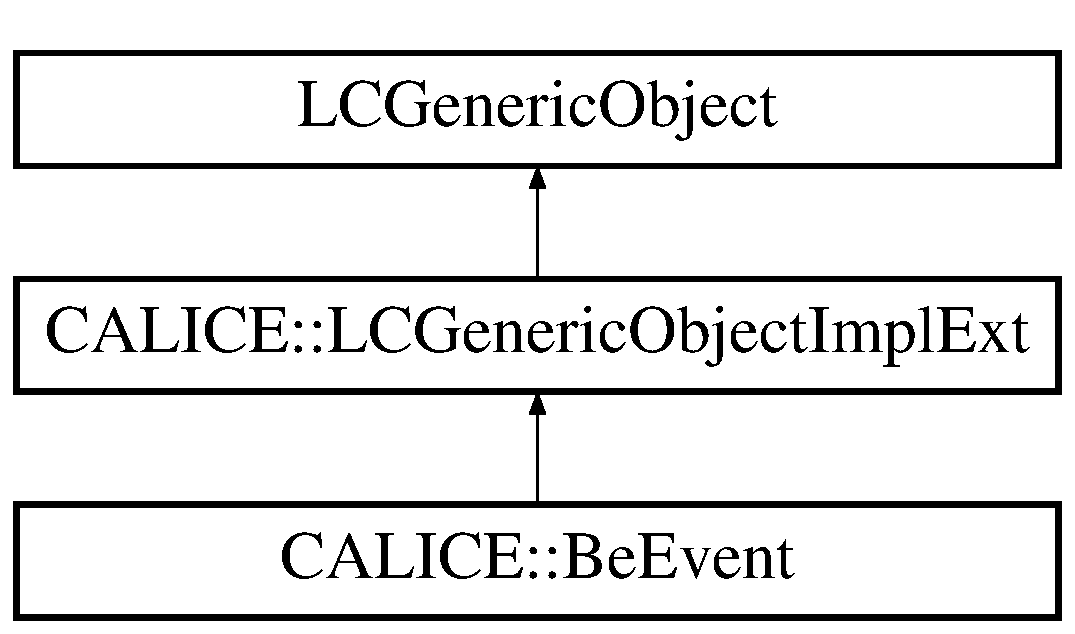
\includegraphics[height=3.000000cm]{classCALICE_1_1BeEvent}
\end{center}
\end{figure}
\subsection*{Public Member Functions}
\begin{DoxyCompactItemize}
\item 
{\bf Be\-Event} ()\label{classCALICE_1_1BeEvent_a2097c6cad17364e073130b88759d4395}

\begin{DoxyCompactList}\small\item\em Simple Constructor. \end{DoxyCompactList}\item 
{\bf Be\-Event} (unsigned int board\-\_\-id)
\begin{DoxyCompactList}\small\item\em Useful\-Constructor. \end{DoxyCompactList}\item 
{\bf Be\-Event} (L\-C\-Object $\ast${\bf obj})\label{classCALICE_1_1BeEvent_aa434832dc8f050ab7d92ea2a90e3a2fa}

\begin{DoxyCompactList}\small\item\em 'Copy constructor' needed to interpret L\-C\-Collection read from file/database. \end{DoxyCompactList}\item 
{\bf Be\-Event} \& {\bf set\-Board\-I\-D} (int board\-I\-D)
\begin{DoxyCompactList}\small\item\em Set the packed board id. \end{DoxyCompactList}\item 
int {\bf get\-Board\-I\-D} () const \label{classCALICE_1_1BeEvent_a257d5c382c76e453d576c99b4785811d}

\begin{DoxyCompactList}\small\item\em Get the board id. \end{DoxyCompactList}\item 
{\bf Be\-Event} \& {\bf set\-Record\-Label} (int label)\label{classCALICE_1_1BeEvent_ab860bbf02c55df7b26c2e9335056a21a}

\begin{DoxyCompactList}\small\item\em Set the Record Label. \end{DoxyCompactList}\item 
short {\bf get\-Record\-Label} () const \label{classCALICE_1_1BeEvent_a9cc54e7581f285b926a192836e904e86}

\begin{DoxyCompactList}\small\item\em Return the Record Label. \end{DoxyCompactList}\item 
{\bf Be\-Event} \& {\bf set\-Status\-Word} (int status)\label{classCALICE_1_1BeEvent_a052f9cb87c190b8137d6ad09e676af1f}

\begin{DoxyCompactList}\small\item\em Set the status word. \end{DoxyCompactList}\item 
int {\bf get\-Status\-Word} () const \label{classCALICE_1_1BeEvent_afffb8609964ae7e46d4eb7c55d6cac08}

\begin{DoxyCompactList}\small\item\em Get the status word. \end{DoxyCompactList}\item 
{\bf Be\-Event} \& {\bf set\-L1a\-Counter} (int l1acounter)\label{classCALICE_1_1BeEvent_ad4dec434b6ae2f78e9db131d26b6330f}

\begin{DoxyCompactList}\small\item\em Set the l1acounter This number is used to check integrity of trigger counters. \end{DoxyCompactList}\item 
int {\bf get\-L1a\-Counter} () const \label{classCALICE_1_1BeEvent_a3bb48d738f07c16324f75e5f3f6594d6}

\begin{DoxyCompactList}\small\item\em Get the l1acounter. \end{DoxyCompactList}\item 
{\bf Be\-Event} \& {\bf set\-Bx\-Counter} (int bxcount)\label{classCALICE_1_1BeEvent_a94fe845cc1ced1dc5743f784f6092bfa}

\begin{DoxyCompactList}\small\item\em Set the bxcounter (bunch crossing !?) \end{DoxyCompactList}\item 
int {\bf get\-Bx\-Counter} () const \label{classCALICE_1_1BeEvent_a85aad5b07a8644221039c50f47c9cfe2}

\begin{DoxyCompactList}\small\item\em Get the bxcounter. \end{DoxyCompactList}\item 
{\bf Be\-Event} \& {\bf set\-Qdr\-Frame\-Counter} (int qdrframecount)\label{classCALICE_1_1BeEvent_abd097e21aaa8d7ac65f473186ec0ec6a}

\begin{DoxyCompactList}\small\item\em Set the Qdr\-Frame\-Counter (Whatever this is ...) \end{DoxyCompactList}\item 
int {\bf get\-Qdr\-Frame\-Counter} () const \label{classCALICE_1_1BeEvent_aef1af66fdeecc7b3e78b6e164681341a}

\begin{DoxyCompactList}\small\item\em Get the Qdr\-Frame\-Counter. \end{DoxyCompactList}\item 
{\bf Be\-Event} \& {\bf set\-Qdr\-Data\-Counter} (int qdrdatacount)\label{classCALICE_1_1BeEvent_ad085e6f2c86bfc12a9c450f55f6a65f6}

\begin{DoxyCompactList}\small\item\em Set the Qdr\-Data\-Counter (Whatever this is ...) \end{DoxyCompactList}\item 
int {\bf get\-Qdr\-Data\-Counter} () const \label{classCALICE_1_1BeEvent_ad917495373bd3b1f6261f0043aca87e0}

\begin{DoxyCompactList}\small\item\em Get the Qdr\-Data\-Counter. \end{DoxyCompactList}\item 
{\bf Be\-Event} \& {\bf set\-Total\-Frame\-Counter} (int totalframecount)\label{classCALICE_1_1BeEvent_accec6ea69ebb86a919ea63115ef9ee90}

\begin{DoxyCompactList}\small\item\em Set the Total\-Frame\-Counter (Whatever this is ...) \end{DoxyCompactList}\item 
int {\bf get\-Total\-Frame\-Counter} () const \label{classCALICE_1_1BeEvent_afbe2088acfa3d8d5a4301d66c9bec655}

\begin{DoxyCompactList}\small\item\em Get the Total\-Frame\-Counter. \end{DoxyCompactList}\item 
void {\bf print} (std\-::ostream \&os)\label{classCALICE_1_1BeEvent_a9554fd6824f75d8bfbfa3183ba8469b1}

\begin{DoxyCompactList}\small\item\em Convenient print method. \end{DoxyCompactList}\item 
const std\-::string {\bfseries get\-Type\-Name} () const \label{classCALICE_1_1BeEvent_a1a9609c2a147fa44055bc3aae63d64c6}

\item 
const std\-::string {\bf get\-Data\-Description} () const \label{classCALICE_1_1BeEvent_a271ed21e4fc8b27bffd8ba9cf3c7d31b}

\begin{DoxyCompactList}\small\item\em Return a brief description of the data members. \end{DoxyCompactList}\end{DoxyCompactItemize}
\subsection*{Additional Inherited Members}


\subsection{Detailed Description}
Stores the trigger history (i.\-e. 

fifo content).when it appears in the front end as realized for runs starting in May 2006 (Ask Paul for firmware version) in older versions of the D\-A\-Q these data came along wiith the Be\-Trg\-Event\-Data which still contains information related to the data handled by the present interface class.

To acces the configuration\-: 
\begin{DoxyPre}
  void processEvent(LCEvent *event)  \{
      try \{
       // string \_colName = "BeTrgEventData"
       LCCollection *col=event->getCollection(\_colName);
       for (unsigned int element\_i=0; element\_i<col->getNumberOfElements(); element\_i++) \{
          \doxyref{BeEvent}{p.}{classCALICE_1_1BeEvent} event(col->getElementAt(element\_i));\end{DoxyPre}



\begin{DoxyPre}       \}
  \}
\end{DoxyPre}


\begin{DoxyAuthor}{Author}
R. P�schl (L\-A\-L Orsay) 
\end{DoxyAuthor}
\begin{DoxyDate}{Date}
Jul 2006 
\end{DoxyDate}


Definition at line 58 of file Be\-Event.\-hh.



\subsection{Constructor \& Destructor Documentation}
\index{C\-A\-L\-I\-C\-E\-::\-Be\-Event@{C\-A\-L\-I\-C\-E\-::\-Be\-Event}!Be\-Event@{Be\-Event}}
\index{Be\-Event@{Be\-Event}!CALICE::BeEvent@{C\-A\-L\-I\-C\-E\-::\-Be\-Event}}
\subsubsection[{Be\-Event}]{\setlength{\rightskip}{0pt plus 5cm}C\-A\-L\-I\-C\-E\-::\-Be\-Event\-::\-Be\-Event (
\begin{DoxyParamCaption}
\item[{unsigned int}]{board\-\_\-id}
\end{DoxyParamCaption}
)\hspace{0.3cm}{\ttfamily [inline]}}\label{classCALICE_1_1BeEvent_a52f929c3fccdded286f6bfb5f3989f09}


Useful\-Constructor. 


\begin{DoxyParams}{Parameters}
{\em board\-\_\-id} & the packed board id (\doxyref{C\-A\-L\-I\-C\-E\-::\-Board\-I\-D}{p.}{classCALICE_1_1BoardID}). \\
\hline
\end{DoxyParams}


Definition at line 80 of file Be\-Event.\-hh.



\subsection{Member Function Documentation}
\index{C\-A\-L\-I\-C\-E\-::\-Be\-Event@{C\-A\-L\-I\-C\-E\-::\-Be\-Event}!set\-Board\-I\-D@{set\-Board\-I\-D}}
\index{set\-Board\-I\-D@{set\-Board\-I\-D}!CALICE::BeEvent@{C\-A\-L\-I\-C\-E\-::\-Be\-Event}}
\subsubsection[{set\-Board\-I\-D}]{\setlength{\rightskip}{0pt plus 5cm}{\bf Be\-Event}\& C\-A\-L\-I\-C\-E\-::\-Be\-Event\-::set\-Board\-I\-D (
\begin{DoxyParamCaption}
\item[{int}]{board\-I\-D}
\end{DoxyParamCaption}
)\hspace{0.3cm}{\ttfamily [inline]}}\label{classCALICE_1_1BeEvent_a63f17cd05b53cb5c3ec91432c54b8ccc}


Set the packed board id. 

\begin{DoxySeeAlso}{See Also}
\doxyref{Board\-I\-D}{p.}{classCALICE_1_1BoardID} 
\end{DoxySeeAlso}


Definition at line 108 of file Be\-Event.\-hh.



The documentation for this class was generated from the following file\-:\begin{DoxyCompactItemize}
\item 
Be\-Event.\-hh\end{DoxyCompactItemize}

\section{C\-A\-L\-I\-C\-E\-:\-:Be\-Trg\-Conf Class Reference}
\label{classCALICE_1_1BeTrgConf}\index{C\-A\-L\-I\-C\-E\-::\-Be\-Trg\-Conf@{C\-A\-L\-I\-C\-E\-::\-Be\-Trg\-Conf}}


Stores the configuration data of the trigger.  




{\ttfamily \#include $<$Be\-Trg\-Conf.\-hh$>$}

Inheritance diagram for C\-A\-L\-I\-C\-E\-:\-:Be\-Trg\-Conf\-:\begin{figure}[H]
\begin{center}
\leavevmode
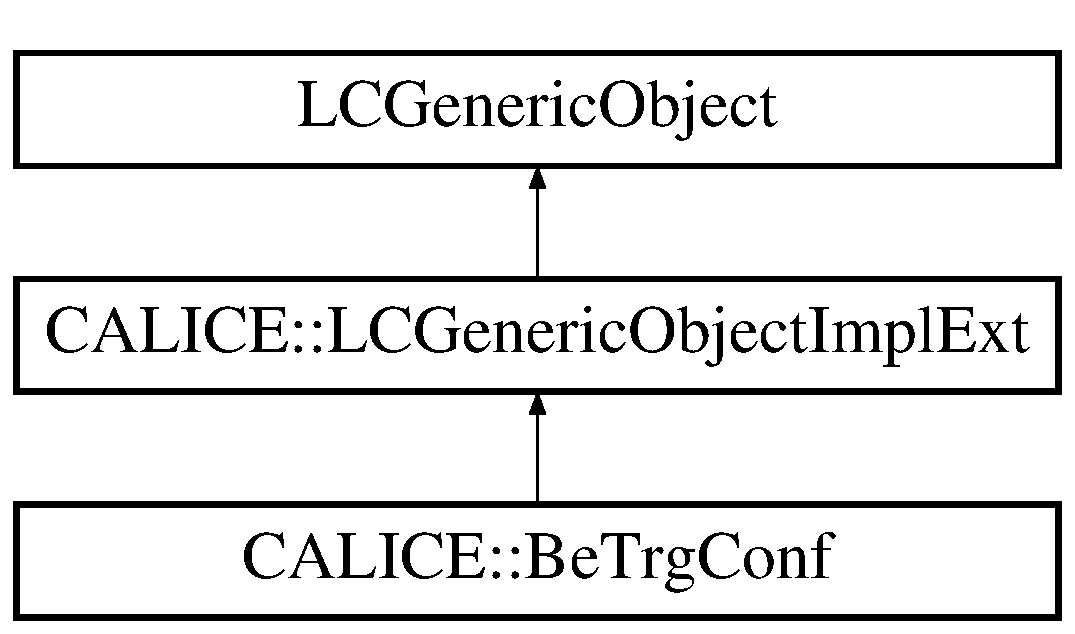
\includegraphics[height=3.000000cm]{classCALICE_1_1BeTrgConf}
\end{center}
\end{figure}
\subsection*{Public Member Functions}
\begin{DoxyCompactItemize}
\item 
{\bf Be\-Trg\-Conf} ()\label{classCALICE_1_1BeTrgConf_a8c09539bda8db3784aae4fbcbcb0ec3f}

\begin{DoxyCompactList}\small\item\em Default Constructor. \end{DoxyCompactList}\item 
{\bf Be\-Trg\-Conf} (int board\-I\-D)
\begin{DoxyCompactList}\small\item\em Ctor. \end{DoxyCompactList}\item 
{\bf Be\-Trg\-Conf} (L\-C\-Object $\ast${\bf obj})\label{classCALICE_1_1BeTrgConf_aa6bbe7ee49bfb432a38a8425fddd3c45}

\begin{DoxyCompactList}\small\item\em 'Copy constructor' needed to interpret L\-C\-Collection read from file/database. \end{DoxyCompactList}\item 
{\bf Be\-Trg\-Conf} \& {\bf set\-Board\-I\-D} (int board\-I\-D)
\begin{DoxyCompactList}\small\item\em set the packed board id. \end{DoxyCompactList}\item 
int {\bf get\-Board\-I\-D} () const \label{classCALICE_1_1BeTrgConf_a332e453076685a181fc82b50782a89f2}

\begin{DoxyCompactList}\small\item\em Information on the F\-E chip the data was received. \end{DoxyCompactList}\item 
void {\bf set\-Record\-Label} (int label)\label{classCALICE_1_1BeTrgConf_a75c2b5f2bdf803500688e0e427545ac5}

\begin{DoxyCompactList}\small\item\em Set the Record Label. \end{DoxyCompactList}\item 
short {\bf get\-Record\-Label} () const \label{classCALICE_1_1BeTrgConf_a3a35836bbb8aa32bcba88d0bbbed2686}

\begin{DoxyCompactList}\small\item\em Return the Record Label. \end{DoxyCompactList}\item 
{\bf Be\-Trg\-Conf} \& {\bf set\-Input\-Enable\-Mask} (int input\-\_\-enable)
\begin{DoxyCompactList}\small\item\em Set the trigger enable bit mask. \end{DoxyCompactList}\item 
int {\bf get\-Input\-Enable\-Mask} () const 
\begin{DoxyCompactList}\small\item\em Get the trigger enable bit mask. \end{DoxyCompactList}\item 
{\bf Be\-Trg\-Conf} \& {\bf set\-Oscillator\-Enable} (int osc\-\_\-enable)\label{classCALICE_1_1BeTrgConf_ac5c442bfe4a6d5d8da543c5444453491}

\begin{DoxyCompactList}\small\item\em Set Oscillator Enable. \end{DoxyCompactList}\item 
int {\bf get\-Oscillator\-Enable} () const \label{classCALICE_1_1BeTrgConf_a786f6d987d88cfff6be350d8d2da72b6}

\begin{DoxyCompactList}\small\item\em Get Oscillator Enable. \end{DoxyCompactList}\item 
{\bf Be\-Trg\-Conf} \& {\bf set\-General\-Enable} (int gen\-\_\-enable)\label{classCALICE_1_1BeTrgConf_a0ec05d6c7bcff2ba528ecbfd3ba02c1e}

\begin{DoxyCompactList}\small\item\em Set General Enable. \end{DoxyCompactList}\item 
int {\bf get\-General\-Enable} () const \label{classCALICE_1_1BeTrgConf_a4c4a9313bba8a0ed7f81092c8f6f1fec}

\begin{DoxyCompactList}\small\item\em Get General Enable. \end{DoxyCompactList}\item 
{\bf Be\-Trg\-Conf} \& {\bf set\-Oscillation\-Period} (int oscillation\-\_\-period)\label{classCALICE_1_1BeTrgConf_a03be1fd0409f19b3bf6b237a4b551e4e}

\begin{DoxyCompactList}\small\item\em Set the oscillation period. \end{DoxyCompactList}\item 
int {\bf get\-Oscillation\-Period} () const \label{classCALICE_1_1BeTrgConf_ac84ad8d502d2306e9380666a870c60ae}

\begin{DoxyCompactList}\small\item\em Get the oscillation period. \end{DoxyCompactList}\item 
{\bf Be\-Trg\-Conf} \& {\bf set\-Burst\-Counter} (int burst\-\_\-count)\label{classCALICE_1_1BeTrgConf_a9ffc7c295209cf416ed76e3e161f5ad2}

\begin{DoxyCompactList}\small\item\em Set the burst counter. \end{DoxyCompactList}\item 
int {\bf get\-Burst\-Counter} () const \label{classCALICE_1_1BeTrgConf_af28d7356fda3f116f34dabd50d52f798}

\begin{DoxyCompactList}\small\item\em Get the burst counter. \end{DoxyCompactList}\item 
{\bf Be\-Trg\-Conf} \& {\bf set\-Configuration} (int config)\label{classCALICE_1_1BeTrgConf_acec95f60250ce4a5d42f9aa7e58db7a7}

\begin{DoxyCompactList}\small\item\em Set the configuration word. \end{DoxyCompactList}\item 
int {\bf get\-Configuration} () const \label{classCALICE_1_1BeTrgConf_a4da9e0491cd18b711e110fc90cabbd57}

\begin{DoxyCompactList}\small\item\em Get the configuration word. \end{DoxyCompactList}\item 
{\bf Be\-Trg\-Conf} \& {\bf set\-Fifo\-Idle\-Depth} (int fifo\-\_\-idle\-\_\-depth)\label{classCALICE_1_1BeTrgConf_ac8baef28684cbcd0a2ffcf4238262d78}

\begin{DoxyCompactList}\small\item\em Set the fifo idle depth. \end{DoxyCompactList}\item 
int {\bf get\-Fifo\-Idle\-Depth} () const \label{classCALICE_1_1BeTrgConf_a2285119c2c7c779f80cfade5ddbd6873}

\begin{DoxyCompactList}\small\item\em Get the fifo idle depth. \end{DoxyCompactList}\item 
{\bf Be\-Trg\-Conf} \& {\bf set\-Busy\-Timeout} (int busy\-\_\-timeout)\label{classCALICE_1_1BeTrgConf_ac4796b32d11183db7c4c26cc27068b04}

\begin{DoxyCompactList}\small\item\em Set the busy time out. \end{DoxyCompactList}\item 
int {\bf get\-Busy\-Timeout} () const \label{classCALICE_1_1BeTrgConf_a92ccb523a8c71cbd92bdd2377120331a}

\begin{DoxyCompactList}\small\item\em Get the busy time out. \end{DoxyCompactList}\item 
{\bf Be\-Trg\-Conf} \& {\bf set\-Burst\-Timeout} (int burst\-\_\-timeout)\label{classCALICE_1_1BeTrgConf_ad1fd90e88ae2d537566b7626fe20f91b}

\begin{DoxyCompactList}\small\item\em Set the burst time out. \end{DoxyCompactList}\item 
int {\bf get\-Burst\-Timeout} () const \label{classCALICE_1_1BeTrgConf_ab7dc9b50b96c180c995e16a0a264acdb}

\begin{DoxyCompactList}\small\item\em Get the burst time out. \end{DoxyCompactList}\item 
{\bf Be\-Trg\-Conf} \& {\bf set\-And\-Enable} (int and\-\_\-enable, int pos)\label{classCALICE_1_1BeTrgConf_a3030bed7c53e0be53ffe16ade5551c8b}

\begin{DoxyCompactList}\small\item\em Set the and\-Enable. \end{DoxyCompactList}\item 
int {\bf get\-And\-Enable} (int pos) const \label{classCALICE_1_1BeTrgConf_a5eff0a3b3e4cc9d68b1de91fd91ed519}

\begin{DoxyCompactList}\small\item\em Get the and Enable. \end{DoxyCompactList}\item 
{\bf Be\-Trg\-Conf} \& {\bf set\-Ext\-Beam\-Mode} (int ext\-\_\-beammode)\label{classCALICE_1_1BeTrgConf_a2d67e0ec00b152680779250acccb556b}

\begin{DoxyCompactList}\small\item\em Set the ext\-Beam Mode. \end{DoxyCompactList}\item 
int {\bf get\-Ext\-Beam\-Mode} () const \label{classCALICE_1_1BeTrgConf_a3c292917f3b29f5ef1a771ad8f1f4f7b}

\begin{DoxyCompactList}\small\item\em Get the ext\-Beam Mode. \end{DoxyCompactList}\item 
{\bf Be\-Trg\-Conf} \& {\bf set\-Input\-Invert} (int input\-\_\-invert)\label{classCALICE_1_1BeTrgConf_aada94ccc553d5cda4b6cf1a2cf173601}

\begin{DoxyCompactList}\small\item\em Set the input invert. \end{DoxyCompactList}\item 
int {\bf get\-Input\-Invert} () const \label{classCALICE_1_1BeTrgConf_a3b4aeee59a32fda0efa23fcfa3327f77}

\begin{DoxyCompactList}\small\item\em Get the input invert. \end{DoxyCompactList}\item 
{\bf Be\-Trg\-Conf} \& {\bf set\-Qdr\-Configuration} (int qdr\-\_\-config)\label{classCALICE_1_1BeTrgConf_a9b707b4d34d920e835988e48ded4cc37}

\begin{DoxyCompactList}\small\item\em Set the qdr configuration. \end{DoxyCompactList}\item 
int {\bf get\-Qdr\-Configuration} () const \label{classCALICE_1_1BeTrgConf_a8879baa5b1fc4d073b11d6b065a73e7d}

\begin{DoxyCompactList}\small\item\em Get the qdr configuration. \end{DoxyCompactList}\item 
{\bf Be\-Trg\-Conf} \& {\bf set\-Sequencer\-Control} (int sequence\-\_\-contr)\label{classCALICE_1_1BeTrgConf_a4583754d7a4cf65c1fb86d29ea836cac}

\begin{DoxyCompactList}\small\item\em Set the sequencer control. \end{DoxyCompactList}\item 
int {\bf get\-Sequencer\-Control} () const \label{classCALICE_1_1BeTrgConf_adb6f6981514a038e70c2e479240fdb3f}

\begin{DoxyCompactList}\small\item\em Get the sequencer control. \end{DoxyCompactList}\item 
void {\bf print} (std\-::ostream \&os)\label{classCALICE_1_1BeTrgConf_a986684df66d456e9275f711d59c913ed}

\begin{DoxyCompactList}\small\item\em Convenient print method. \end{DoxyCompactList}\item 
const std\-::string {\bf get\-Type\-Name} () const \label{classCALICE_1_1BeTrgConf_ab51e1dcd328cea0821792d00e49ef504}

\begin{DoxyCompactList}\small\item\em Return the type of the class. \end{DoxyCompactList}\item 
const std\-::string {\bf get\-Data\-Description} () const \label{classCALICE_1_1BeTrgConf_a396979e8da1cf0d9e19930e75fd8c858}

\begin{DoxyCompactList}\small\item\em Return a brief description of the data members. \end{DoxyCompactList}\end{DoxyCompactItemize}
\subsection*{Additional Inherited Members}


\subsection{Detailed Description}
Stores the configuration data of the trigger. 

To acces the configuration\-: 
\begin{DoxyPre}
  void BrTrgCondChangeListener(LCCollection *col)  \{
       assert (col->getNumberOfElements()==1)
       \doxyref{BeTrgConf}{p.}{classCALICE_1_1BeTrgConf} conf(col->getElementAt(0));\end{DoxyPre}



\begin{DoxyPre}       UInt\_t enable\_mask=conf.getEnableMask();
  \}
\end{DoxyPre}


\begin{DoxySeeAlso}{See Also}
\doxyref{Conditions\-Change\-Delegator}{p.}{classCALICE_1_1ConditionsChangeDelegator} 
\end{DoxySeeAlso}
\begin{DoxyAuthor}{Author}
G�tz Gaycken L\-L\-R (Ecole Polytechnique) 
\end{DoxyAuthor}
\begin{DoxyDate}{Date}
Sep 2005 
\end{DoxyDate}


Definition at line 76 of file Be\-Trg\-Conf.\-hh.



\subsection{Constructor \& Destructor Documentation}
\index{C\-A\-L\-I\-C\-E\-::\-Be\-Trg\-Conf@{C\-A\-L\-I\-C\-E\-::\-Be\-Trg\-Conf}!Be\-Trg\-Conf@{Be\-Trg\-Conf}}
\index{Be\-Trg\-Conf@{Be\-Trg\-Conf}!CALICE::BeTrgConf@{C\-A\-L\-I\-C\-E\-::\-Be\-Trg\-Conf}}
\subsubsection[{Be\-Trg\-Conf}]{\setlength{\rightskip}{0pt plus 5cm}C\-A\-L\-I\-C\-E\-::\-Be\-Trg\-Conf\-::\-Be\-Trg\-Conf (
\begin{DoxyParamCaption}
\item[{int}]{board\-I\-D}
\end{DoxyParamCaption}
)\hspace{0.3cm}{\ttfamily [inline]}}\label{classCALICE_1_1BeTrgConf_a5af9732e0e1783bfc26a513911e9d85e}


Ctor. 


\begin{DoxyParams}{Parameters}
{\em board\-I\-D} & the packed board id (\doxyref{Board\-I\-D}{p.}{classCALICE_1_1BoardID}). \\
\hline
\end{DoxyParams}


Definition at line 86 of file Be\-Trg\-Conf.\-hh.



\subsection{Member Function Documentation}
\index{C\-A\-L\-I\-C\-E\-::\-Be\-Trg\-Conf@{C\-A\-L\-I\-C\-E\-::\-Be\-Trg\-Conf}!get\-Input\-Enable\-Mask@{get\-Input\-Enable\-Mask}}
\index{get\-Input\-Enable\-Mask@{get\-Input\-Enable\-Mask}!CALICE::BeTrgConf@{C\-A\-L\-I\-C\-E\-::\-Be\-Trg\-Conf}}
\subsubsection[{get\-Input\-Enable\-Mask}]{\setlength{\rightskip}{0pt plus 5cm}int C\-A\-L\-I\-C\-E\-::\-Be\-Trg\-Conf\-::get\-Input\-Enable\-Mask (
\begin{DoxyParamCaption}
{}
\end{DoxyParamCaption}
) const\hspace{0.3cm}{\ttfamily [inline]}}\label{classCALICE_1_1BeTrgConf_ac38488bad25a502a3b0c15d0b5030efc}


Get the trigger enable bit mask. 

For each aenabled trigger a bit is set. The meaning of the bits is defined by conditions data. \begin{DoxySeeAlso}{See Also}
Trigger\-Mask. 
\end{DoxySeeAlso}


Definition at line 128 of file Be\-Trg\-Conf.\-hh.

\index{C\-A\-L\-I\-C\-E\-::\-Be\-Trg\-Conf@{C\-A\-L\-I\-C\-E\-::\-Be\-Trg\-Conf}!set\-Board\-I\-D@{set\-Board\-I\-D}}
\index{set\-Board\-I\-D@{set\-Board\-I\-D}!CALICE::BeTrgConf@{C\-A\-L\-I\-C\-E\-::\-Be\-Trg\-Conf}}
\subsubsection[{set\-Board\-I\-D}]{\setlength{\rightskip}{0pt plus 5cm}{\bf Be\-Trg\-Conf}\& C\-A\-L\-I\-C\-E\-::\-Be\-Trg\-Conf\-::set\-Board\-I\-D (
\begin{DoxyParamCaption}
\item[{int}]{board\-I\-D}
\end{DoxyParamCaption}
)\hspace{0.3cm}{\ttfamily [inline]}}\label{classCALICE_1_1BeTrgConf_aebabae2847b682da59cb5e2f5ec15141}


set the packed board id. 

\begin{DoxySeeAlso}{See Also}
\doxyref{Board\-I\-D}{p.}{classCALICE_1_1BoardID} 
\end{DoxySeeAlso}


Definition at line 97 of file Be\-Trg\-Conf.\-hh.

\index{C\-A\-L\-I\-C\-E\-::\-Be\-Trg\-Conf@{C\-A\-L\-I\-C\-E\-::\-Be\-Trg\-Conf}!set\-Input\-Enable\-Mask@{set\-Input\-Enable\-Mask}}
\index{set\-Input\-Enable\-Mask@{set\-Input\-Enable\-Mask}!CALICE::BeTrgConf@{C\-A\-L\-I\-C\-E\-::\-Be\-Trg\-Conf}}
\subsubsection[{set\-Input\-Enable\-Mask}]{\setlength{\rightskip}{0pt plus 5cm}{\bf Be\-Trg\-Conf}\& C\-A\-L\-I\-C\-E\-::\-Be\-Trg\-Conf\-::set\-Input\-Enable\-Mask (
\begin{DoxyParamCaption}
\item[{int}]{input\-\_\-enable}
\end{DoxyParamCaption}
)\hspace{0.3cm}{\ttfamily [inline]}}\label{classCALICE_1_1BeTrgConf_a4adeeec5eb99fe7b5bba2e12cb525c38}


Set the trigger enable bit mask. 

For each aenabled trigger a bit is set. The meaning of the bits is defined by conditions data. \begin{DoxySeeAlso}{See Also}
Trigger\-Mask. 
\end{DoxySeeAlso}


Definition at line 118 of file Be\-Trg\-Conf.\-hh.



The documentation for this class was generated from the following file\-:\begin{DoxyCompactItemize}
\item 
Be\-Trg\-Conf.\-hh\end{DoxyCompactItemize}

\section{C\-A\-L\-I\-C\-E\-:\-:Be\-Trg\-Event Class Reference}
\label{classCALICE_1_1BeTrgEvent}\index{C\-A\-L\-I\-C\-E\-::\-Be\-Trg\-Event@{C\-A\-L\-I\-C\-E\-::\-Be\-Trg\-Event}}


Stores the trigger event data.  




{\ttfamily \#include $<$Be\-Trg\-Event.\-hh$>$}

Inheritance diagram for C\-A\-L\-I\-C\-E\-:\-:Be\-Trg\-Event\-:\begin{figure}[H]
\begin{center}
\leavevmode
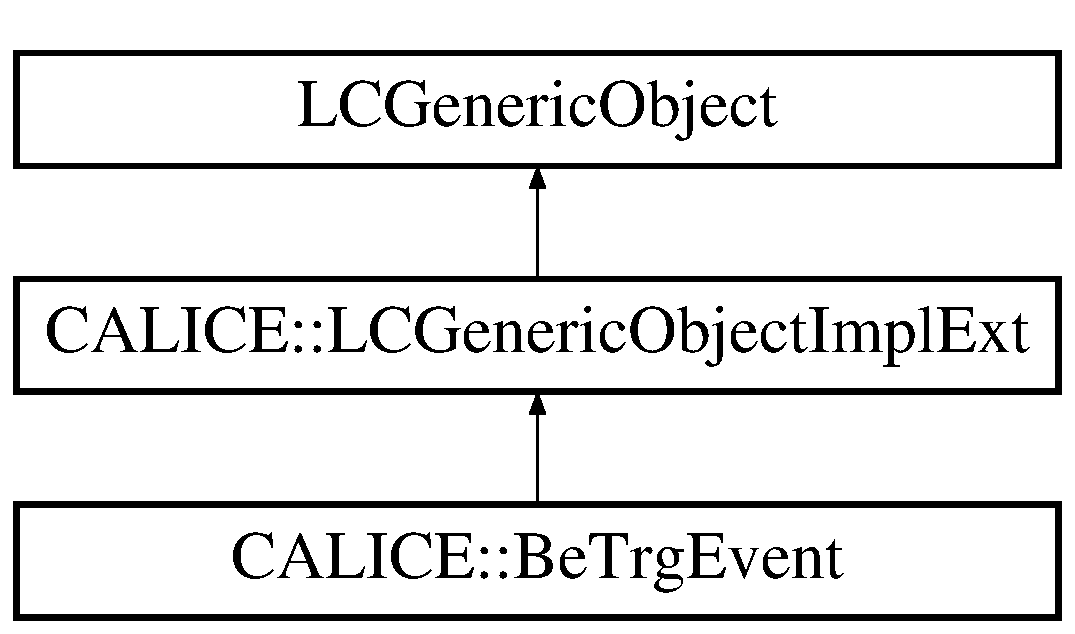
\includegraphics[height=3.000000cm]{classCALICE_1_1BeTrgEvent}
\end{center}
\end{figure}
\subsection*{Public Member Functions}
\begin{DoxyCompactItemize}
\item 
{\bf Be\-Trg\-Event} (unsigned int board\-\_\-id)
\begin{DoxyCompactList}\small\item\em Useful\-Constructor. \end{DoxyCompactList}\item 
{\bf Be\-Trg\-Event} (L\-C\-Object $\ast${\bf obj})\label{classCALICE_1_1BeTrgEvent_aad3ab901206f9cfe9867505455e014fe}

\begin{DoxyCompactList}\small\item\em 'Copy constructor' needed to interpret L\-C\-Collection read from file/database. \end{DoxyCompactList}\item 
{\bf Be\-Trg\-Event} \& {\bf set\-Board\-I\-D} (int board\-I\-D)
\begin{DoxyCompactList}\small\item\em set the packed board id. \end{DoxyCompactList}\item 
int {\bf get\-Board\-I\-D} () const \label{classCALICE_1_1BeTrgEvent_a0a62c75cb07342d47e5298ebfb34f7d8}

\begin{DoxyCompactList}\small\item\em Information on the F\-E chip the data was received. \end{DoxyCompactList}\item 
{\bf Be\-Trg\-Event} \& {\bf set\-Input\-Status} (int input\-\_\-status)
\begin{DoxyCompactList}\small\item\em Set the pre busy trigger counter (what ever that is ;-\/). \end{DoxyCompactList}\item 
int {\bf get\-Input\-Status} () const \label{classCALICE_1_1BeTrgEvent_acaea9fd53c2fd11f7b31db9ea9806658}

\begin{DoxyCompactList}\small\item\em Get the input status. \end{DoxyCompactList}\item 
{\bf Be\-Trg\-Event} \& {\bf set\-Input\-Catch} (int input\-\_\-catch)\label{classCALICE_1_1BeTrgEvent_af1b27f8a852855d164e5f71b7406998c}

\begin{DoxyCompactList}\small\item\em Set the input catch (what ever that is ;-\/). \end{DoxyCompactList}\item 
int {\bf get\-Input\-Catch} () const \label{classCALICE_1_1BeTrgEvent_ae076fd16cf3ee806c64a1d2e82e29f50}

\begin{DoxyCompactList}\small\item\em Get the input catch (what ever that is ;-\/). \end{DoxyCompactList}\item 
{\bf Be\-Trg\-Event} \& {\bf set\-Pre\-Busy\-Catch} (int prebusy\-\_\-catch)
\begin{DoxyCompactList}\small\item\em Set the trigger busy status. \end{DoxyCompactList}\item 
int {\bf get\-Prebusy\-Catch} () const \label{classCALICE_1_1BeTrgEvent_a06df76683895a30404a54912b09d210a}

\begin{DoxyCompactList}\small\item\em Get the prebusy Catch. \end{DoxyCompactList}\item 
{\bf Be\-Trg\-Event} \& {\bf set\-Signal\-Catch} (int signal\-\_\-catch)\label{classCALICE_1_1BeTrgEvent_a8cf5425520f7881a57cb36a959fc256f}

\begin{DoxyCompactList}\small\item\em Set the signal Catch. \end{DoxyCompactList}\item 
int {\bf get\-Signal\-Catch} () const \label{classCALICE_1_1BeTrgEvent_a0afe03ca2e64566c074045563fb62ef9}

\begin{DoxyCompactList}\small\item\em Get the signal Catch. \end{DoxyCompactList}\item 
{\bf Be\-Trg\-Event} \& {\bf set\-Control} (int control)\label{classCALICE_1_1BeTrgEvent_a145c2a82f590cd2350a1f6c5d350c178}

\begin{DoxyCompactList}\small\item\em Set the contrl value. \end{DoxyCompactList}\item 
int {\bf get\-Control} () const \label{classCALICE_1_1BeTrgEvent_acf9e7facc723fe1c420b3cd2c1b4993f}

\begin{DoxyCompactList}\small\item\em Get the control value. \end{DoxyCompactList}\item 
{\bf Be\-Trg\-Event} \& {\bf set\-Initial\-Fifo\-Status} (int initial\-\_\-fifo\-\_\-status)\label{classCALICE_1_1BeTrgEvent_ae2c3ed9c3ebfd484ea022bb308a6faca}

\begin{DoxyCompactList}\small\item\em Set the inital fifo status. \end{DoxyCompactList}\item 
int {\bf get\-Initial\-Fifo\-Status} () const \label{classCALICE_1_1BeTrgEvent_a4359fbafae59cc303c5160f3626c74e6}

\begin{DoxyCompactList}\small\item\em Get the initial fifo status. \end{DoxyCompactList}\item 
{\bf Be\-Trg\-Event} \& {\bf set\-Final\-Fifo\-Status} (int final\-\_\-fifo\-\_\-status)\label{classCALICE_1_1BeTrgEvent_aef331b17a4eca0f054c3379b517c1bbe}

\begin{DoxyCompactList}\small\item\em Set the final fifo status. \end{DoxyCompactList}\item 
int {\bf get\-Final\-Fifo\-Status} () const \label{classCALICE_1_1BeTrgEvent_a7674994d84b63ae049e64fbbae486289}

\begin{DoxyCompactList}\small\item\em Get the final fifo status. \end{DoxyCompactList}\item 
{\bf Be\-Trg\-Event} \& {\bf set\-Fifo\-Word} (unsigned int word\-\_\-index, unsigned int word)
\begin{DoxyCompactList}\small\item\em Set the fifo word. \end{DoxyCompactList}\item 
{\bf Be\-Trg\-Event} \& {\bf set\-All\-Fifo\-Words} (unsigned int n\-\_\-words, const unsigned int $\ast$const word\-\_\-list)
\begin{DoxyCompactList}\small\item\em Set all the fifo words. \end{DoxyCompactList}\item 
int {\bf get\-N\-Fifo\-Words} () const \label{classCALICE_1_1BeTrgEvent_a8dad5638340b3046d0cad0012fe1c03a}

\begin{DoxyCompactList}\small\item\em Get the number of words contained in the fifo. \end{DoxyCompactList}\item 
int {\bf get\-Fifo\-Word} (unsigned int word\-\_\-index) const 
\begin{DoxyCompactList}\small\item\em Get a fifo word. \end{DoxyCompactList}\item 
Int\-Vec \& {\bf get\-Fifo\-Words} (Int\-Vec \&dest) const 
\begin{DoxyCompactList}\small\item\em Get a fifo word. \end{DoxyCompactList}\item 
{\bf Be\-Trg\-Event} \& {\bf set\-Trigger\-Counter} (int trigger\-\_\-counter)\label{classCALICE_1_1BeTrgEvent_ab3751be9202d7dba09f8bbf08ac3aa37}

\begin{DoxyCompactList}\small\item\em Set the trigger counter. \end{DoxyCompactList}\item 
int {\bf get\-Trigger\-Counter} () const \label{classCALICE_1_1BeTrgEvent_a9fcd7bb63d0416bcf6099e7284682419}

\begin{DoxyCompactList}\small\item\em Get the trigger counter. \end{DoxyCompactList}\item 
{\bf Be\-Trg\-Event} \& {\bf set\-Pre\-Busy\-Trigger\-Counter} (int prebusy\-\_\-counter)\label{classCALICE_1_1BeTrgEvent_aaf444986a4b42c9b9b050a2567e0fe4b}

\begin{DoxyCompactList}\small\item\em Set the prebusy Trigger counter. \end{DoxyCompactList}\item 
int {\bf get\-Pre\-Busy\-Trigger\-Counter} () const \label{classCALICE_1_1BeTrgEvent_a4325337c9d9c673d1418b626c273c3f7}

\begin{DoxyCompactList}\small\item\em Get the prebusy trigger counter. \end{DoxyCompactList}\item 
void {\bf print} (std\-::ostream \&os)\label{classCALICE_1_1BeTrgEvent_ab0a9546572d498159435527bf4d9c950}

\begin{DoxyCompactList}\small\item\em Convenient print method. \end{DoxyCompactList}\item 
const std\-::string {\bfseries get\-Type\-Name} () const \label{classCALICE_1_1BeTrgEvent_a7ec78f3a56262534b36eb467b3f56013}

\item 
const std\-::string {\bf get\-Data\-Description} () const \label{classCALICE_1_1BeTrgEvent_a55df9320a60e43187e712b3410317aa5}

\begin{DoxyCompactList}\small\item\em Return a brief description of the data members. \end{DoxyCompactList}\end{DoxyCompactItemize}
\subsection*{Additional Inherited Members}


\subsection{Detailed Description}
Stores the trigger event data. 

To acces the configuration\-: 
\begin{DoxyPre}
  void processEvent(LCEvent *event)  \{
      try \{
       // string \_colName = "BeTrgEventData"
       LCCollection *col=event->getCollection(\_colName);
       for (unsigned int element\_i=0; element\_i<col->getNumberOfElements(); element\_i++) \{
          \doxyref{BeTrgEvent}{p.}{classCALICE_1_1BeTrgEvent} event(col->getElementAt(element\_i));\end{DoxyPre}



\begin{DoxyPre}       \}
  \}
\end{DoxyPre}


\begin{DoxySeeAlso}{See Also}
\doxyref{Conditions\-Change\-Delegator}{p.}{classCALICE_1_1ConditionsChangeDelegator}
\end{DoxySeeAlso}
\begin{DoxyAuthor}{Author}
G�tz Gaycken L\-L\-R (Ecole Polytechnique) 
\end{DoxyAuthor}
\begin{DoxyDate}{Date}
Sep 2005 
\end{DoxyDate}


Definition at line 74 of file Be\-Trg\-Event.\-hh.



\subsection{Constructor \& Destructor Documentation}
\index{C\-A\-L\-I\-C\-E\-::\-Be\-Trg\-Event@{C\-A\-L\-I\-C\-E\-::\-Be\-Trg\-Event}!Be\-Trg\-Event@{Be\-Trg\-Event}}
\index{Be\-Trg\-Event@{Be\-Trg\-Event}!CALICE::BeTrgEvent@{C\-A\-L\-I\-C\-E\-::\-Be\-Trg\-Event}}
\subsubsection[{Be\-Trg\-Event}]{\setlength{\rightskip}{0pt plus 5cm}C\-A\-L\-I\-C\-E\-::\-Be\-Trg\-Event\-::\-Be\-Trg\-Event (
\begin{DoxyParamCaption}
\item[{unsigned int}]{board\-\_\-id}
\end{DoxyParamCaption}
)\hspace{0.3cm}{\ttfamily [inline]}}\label{classCALICE_1_1BeTrgEvent_ab66620b2f1ccf07f5334d37c54fcf77e}


Useful\-Constructor. 


\begin{DoxyParams}{Parameters}
{\em board\-\_\-id} & the packed board id (\doxyref{C\-A\-L\-I\-C\-E\-::\-Board\-I\-D}{p.}{classCALICE_1_1BoardID}). \\
\hline
\end{DoxyParams}


Definition at line 82 of file Be\-Trg\-Event.\-hh.



\subsection{Member Function Documentation}
\index{C\-A\-L\-I\-C\-E\-::\-Be\-Trg\-Event@{C\-A\-L\-I\-C\-E\-::\-Be\-Trg\-Event}!get\-Fifo\-Word@{get\-Fifo\-Word}}
\index{get\-Fifo\-Word@{get\-Fifo\-Word}!CALICE::BeTrgEvent@{C\-A\-L\-I\-C\-E\-::\-Be\-Trg\-Event}}
\subsubsection[{get\-Fifo\-Word}]{\setlength{\rightskip}{0pt plus 5cm}int C\-A\-L\-I\-C\-E\-::\-Be\-Trg\-Event\-::get\-Fifo\-Word (
\begin{DoxyParamCaption}
\item[{unsigned int}]{word\-\_\-index}
\end{DoxyParamCaption}
) const\hspace{0.3cm}{\ttfamily [inline]}}\label{classCALICE_1_1BeTrgEvent_a8c401cd2b6f76c27f2430ce3e4ebf609}


Get a fifo word. 


\begin{DoxyParams}{Parameters}
{\em word\-\_\-index} & of the word in the fifo \\
\hline
\end{DoxyParams}


Definition at line 225 of file Be\-Trg\-Event.\-hh.

\index{C\-A\-L\-I\-C\-E\-::\-Be\-Trg\-Event@{C\-A\-L\-I\-C\-E\-::\-Be\-Trg\-Event}!get\-Fifo\-Words@{get\-Fifo\-Words}}
\index{get\-Fifo\-Words@{get\-Fifo\-Words}!CALICE::BeTrgEvent@{C\-A\-L\-I\-C\-E\-::\-Be\-Trg\-Event}}
\subsubsection[{get\-Fifo\-Words}]{\setlength{\rightskip}{0pt plus 5cm}Int\-Vec\& C\-A\-L\-I\-C\-E\-::\-Be\-Trg\-Event\-::get\-Fifo\-Words (
\begin{DoxyParamCaption}
\item[{Int\-Vec \&}]{dest}
\end{DoxyParamCaption}
) const\hspace{0.3cm}{\ttfamily [inline]}}\label{classCALICE_1_1BeTrgEvent_acb8303a2a3d1c04c260e1ba7c29c5cbc}


Get a fifo word. 


\begin{DoxyParams}{Parameters}
{\em dest} & reference to a vector of integers which will be cleared in filled with the contents of the fifo \\
\hline
\end{DoxyParams}
\begin{DoxyReturn}{Returns}
for convenience a reference to the filled vector (i.\-e. is the one given as argument).
\end{DoxyReturn}
N\-O\-T\-E\-: Unless a vector is needed to pass the data to some function, it is adviced to get the individual values with \doxyref{get\-Fifo\-Word()}{p.}{classCALICE_1_1BeTrgEvent_a8c401cd2b6f76c27f2430ce3e4ebf609} since this avoids copying (On the other hand, each access has the penalty of a virtual function call, so in some cases it might be advantages to make a copy which will allow faster element acces in subsequent calls.) 

Definition at line 246 of file Be\-Trg\-Event.\-hh.

\index{C\-A\-L\-I\-C\-E\-::\-Be\-Trg\-Event@{C\-A\-L\-I\-C\-E\-::\-Be\-Trg\-Event}!set\-All\-Fifo\-Words@{set\-All\-Fifo\-Words}}
\index{set\-All\-Fifo\-Words@{set\-All\-Fifo\-Words}!CALICE::BeTrgEvent@{C\-A\-L\-I\-C\-E\-::\-Be\-Trg\-Event}}
\subsubsection[{set\-All\-Fifo\-Words}]{\setlength{\rightskip}{0pt plus 5cm}{\bf Be\-Trg\-Event}\& C\-A\-L\-I\-C\-E\-::\-Be\-Trg\-Event\-::set\-All\-Fifo\-Words (
\begin{DoxyParamCaption}
\item[{unsigned int}]{n\-\_\-words, }
\item[{const unsigned int $\ast$const}]{word\-\_\-list}
\end{DoxyParamCaption}
)\hspace{0.3cm}{\ttfamily [inline]}}\label{classCALICE_1_1BeTrgEvent_a9f7fbf8c21c3884468b277ef3323af6c}


Set all the fifo words. 


\begin{DoxyParams}{Parameters}
{\em n\-\_\-words} & the number of words in the fifo. \\
\hline
{\em word\-\_\-list} & a pointer to the fifo words. \\
\hline
\end{DoxyParams}


Definition at line 206 of file Be\-Trg\-Event.\-hh.

\index{C\-A\-L\-I\-C\-E\-::\-Be\-Trg\-Event@{C\-A\-L\-I\-C\-E\-::\-Be\-Trg\-Event}!set\-Board\-I\-D@{set\-Board\-I\-D}}
\index{set\-Board\-I\-D@{set\-Board\-I\-D}!CALICE::BeTrgEvent@{C\-A\-L\-I\-C\-E\-::\-Be\-Trg\-Event}}
\subsubsection[{set\-Board\-I\-D}]{\setlength{\rightskip}{0pt plus 5cm}{\bf Be\-Trg\-Event}\& C\-A\-L\-I\-C\-E\-::\-Be\-Trg\-Event\-::set\-Board\-I\-D (
\begin{DoxyParamCaption}
\item[{int}]{board\-I\-D}
\end{DoxyParamCaption}
)\hspace{0.3cm}{\ttfamily [inline]}}\label{classCALICE_1_1BeTrgEvent_a70ffd8782e93479e543253bd331c8a15}


set the packed board id. 

\begin{DoxySeeAlso}{See Also}
\doxyref{Board\-I\-D}{p.}{classCALICE_1_1BoardID} 
\end{DoxySeeAlso}


Definition at line 98 of file Be\-Trg\-Event.\-hh.

\index{C\-A\-L\-I\-C\-E\-::\-Be\-Trg\-Event@{C\-A\-L\-I\-C\-E\-::\-Be\-Trg\-Event}!set\-Fifo\-Word@{set\-Fifo\-Word}}
\index{set\-Fifo\-Word@{set\-Fifo\-Word}!CALICE::BeTrgEvent@{C\-A\-L\-I\-C\-E\-::\-Be\-Trg\-Event}}
\subsubsection[{set\-Fifo\-Word}]{\setlength{\rightskip}{0pt plus 5cm}{\bf Be\-Trg\-Event}\& C\-A\-L\-I\-C\-E\-::\-Be\-Trg\-Event\-::set\-Fifo\-Word (
\begin{DoxyParamCaption}
\item[{unsigned int}]{word\-\_\-index, }
\item[{unsigned int}]{word}
\end{DoxyParamCaption}
)\hspace{0.3cm}{\ttfamily [inline]}}\label{classCALICE_1_1BeTrgEvent_a318de8225e762747bcb7bc2c168d6324}


Set the fifo word. 


\begin{DoxyParams}{Parameters}
{\em word\-\_\-index} & of the word in the fifo. \\
\hline
{\em word} & the value of the word. \\
\hline
\end{DoxyParams}


Definition at line 199 of file Be\-Trg\-Event.\-hh.

\index{C\-A\-L\-I\-C\-E\-::\-Be\-Trg\-Event@{C\-A\-L\-I\-C\-E\-::\-Be\-Trg\-Event}!set\-Input\-Status@{set\-Input\-Status}}
\index{set\-Input\-Status@{set\-Input\-Status}!CALICE::BeTrgEvent@{C\-A\-L\-I\-C\-E\-::\-Be\-Trg\-Event}}
\subsubsection[{set\-Input\-Status}]{\setlength{\rightskip}{0pt plus 5cm}{\bf Be\-Trg\-Event}\& C\-A\-L\-I\-C\-E\-::\-Be\-Trg\-Event\-::set\-Input\-Status (
\begin{DoxyParamCaption}
\item[{int}]{input\-\_\-status}
\end{DoxyParamCaption}
)\hspace{0.3cm}{\ttfamily [inline]}}\label{classCALICE_1_1BeTrgEvent_a0425fc76da285989b2baf35e561c31ba}


Set the pre busy trigger counter (what ever that is ;-\/). 

Get the pre busy trigger counter (what ever that is ;-\/).Set the trigger counter.\-Get the trigger counter.\-Set the input status. 

Definition at line 124 of file Be\-Trg\-Event.\-hh.

\index{C\-A\-L\-I\-C\-E\-::\-Be\-Trg\-Event@{C\-A\-L\-I\-C\-E\-::\-Be\-Trg\-Event}!set\-Pre\-Busy\-Catch@{set\-Pre\-Busy\-Catch}}
\index{set\-Pre\-Busy\-Catch@{set\-Pre\-Busy\-Catch}!CALICE::BeTrgEvent@{C\-A\-L\-I\-C\-E\-::\-Be\-Trg\-Event}}
\subsubsection[{set\-Pre\-Busy\-Catch}]{\setlength{\rightskip}{0pt plus 5cm}{\bf Be\-Trg\-Event}\& C\-A\-L\-I\-C\-E\-::\-Be\-Trg\-Event\-::set\-Pre\-Busy\-Catch (
\begin{DoxyParamCaption}
\item[{int}]{prebusy\-\_\-catch}
\end{DoxyParamCaption}
)\hspace{0.3cm}{\ttfamily [inline]}}\label{classCALICE_1_1BeTrgEvent_a4ba6c3c2e405960a6d7694f1773a4224}


Set the trigger busy status. 

Get the trigger busy status.\-Set the prebusy Catch. 

Definition at line 151 of file Be\-Trg\-Event.\-hh.



The documentation for this class was generated from the following file\-:\begin{DoxyCompactItemize}
\item 
Be\-Trg\-Event.\-hh\end{DoxyCompactItemize}

\section{C\-A\-L\-I\-C\-E\-:\-:Be\-Trg\-Poll\-Data Class Reference}
\label{classCALICE_1_1BeTrgPollData}\index{C\-A\-L\-I\-C\-E\-::\-Be\-Trg\-Poll\-Data@{C\-A\-L\-I\-C\-E\-::\-Be\-Trg\-Poll\-Data}}


Class to store info on trigger polling, This is useful to detect a softtrigger among e.\-g.  




{\ttfamily \#include $<$Be\-Trg\-Poll\-Data.\-hh$>$}

Inheritance diagram for C\-A\-L\-I\-C\-E\-:\-:Be\-Trg\-Poll\-Data\-:\begin{figure}[H]
\begin{center}
\leavevmode
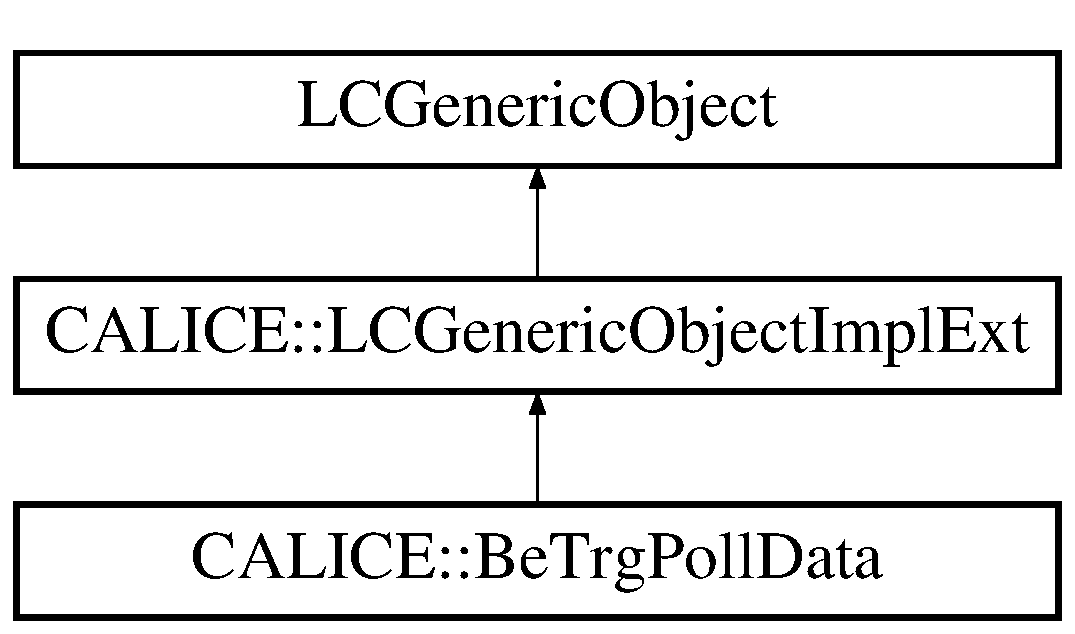
\includegraphics[height=3.000000cm]{classCALICE_1_1BeTrgPollData}
\end{center}
\end{figure}
\subsection*{Public Member Functions}
\begin{DoxyCompactItemize}
\item 
{\bf Be\-Trg\-Poll\-Data} ()\label{classCALICE_1_1BeTrgPollData_a057354fffb3480442ed0c56bd161d84a}

\begin{DoxyCompactList}\small\item\em Default Constructor. \end{DoxyCompactList}\item 
{\bf Be\-Trg\-Poll\-Data} (L\-C\-Object $\ast${\bf obj})\label{classCALICE_1_1BeTrgPollData_a058b62681a118d4cc5ffce52916cbcc5}

\begin{DoxyCompactList}\small\item\em A copy constructor. \end{DoxyCompactList}\item 
virtual {\bf $\sim$\-Be\-Trg\-Poll\-Data} ()\label{classCALICE_1_1BeTrgPollData_a5c9f105b897e0636f88eeb449694c11d}

\begin{DoxyCompactList}\small\item\em The destructor. \end{DoxyCompactList}\item 
{\bf Be\-Trg\-Poll\-Data} \& {\bf set\-Board\-I\-D} (int board\-I\-D)
\begin{DoxyCompactList}\small\item\em set the packed board id. \end{DoxyCompactList}\item 
int {\bf get\-Board\-I\-D} () const \label{classCALICE_1_1BeTrgPollData_a5141403dac81c51d98f1f84633756c7d}

\begin{DoxyCompactList}\small\item\em get the board id \end{DoxyCompactList}\item 
{\bf Be\-Trg\-Poll\-Data} \& {\bf set\-Record\-Label} (int label)\label{classCALICE_1_1BeTrgPollData_a7ff5667fae7e50368b2d56fa395bcfcc}

\begin{DoxyCompactList}\small\item\em Set the Record Label. \end{DoxyCompactList}\item 
short {\bf get\-Record\-Label} () const \label{classCALICE_1_1BeTrgPollData_aa28da3731e1d2ee372d3bdab3595610f}

\begin{DoxyCompactList}\small\item\em Return the Record Label. \end{DoxyCompactList}\item 
{\bf Be\-Trg\-Poll\-Data} \& {\bf set\-Start\-Time} (struct tm $\ast$start\-Time, int start\-Timemus)\label{classCALICE_1_1BeTrgPollData_a9a72f0707c23960f0ff1bc815590e327}

\begin{DoxyCompactList}\small\item\em set the start time We store Year, Month, Day and Hour, Minute, Second and microsceconds seperately We store U\-T\-C!!!! \end{DoxyCompactList}\item 
L\-C\-Time {\bf get\-Start\-Time} ()\label{classCALICE_1_1BeTrgPollData_ab10dba32878399a29531258a4b9c861c}

\begin{DoxyCompactList}\small\item\em returns the start time \end{DoxyCompactList}\item 
{\bf Be\-Trg\-Poll\-Data} \& {\bf set\-End\-Time} (struct tm $\ast$end\-Time, int end\-Timemus)\label{classCALICE_1_1BeTrgPollData_a20bde7a4d727cb651db1060c8950b262}

\begin{DoxyCompactList}\small\item\em set the end time (see set of start time) \end{DoxyCompactList}\item 
L\-C\-Time {\bf get\-End\-Time} ()\label{classCALICE_1_1BeTrgPollData_a6b6279c993919741cbd248cc1e13b4d1}

\begin{DoxyCompactList}\small\item\em returns the end time (see start time) \end{DoxyCompactList}\item 
{\bf Be\-Trg\-Poll\-Data} \& {\bf set\-Maximum\-Time} (int max\-Timesec, int max\-Timemus)\label{classCALICE_1_1BeTrgPollData_ad5db0ea39364cb7ffc2c49402ea9e01e}

\begin{DoxyCompactList}\small\item\em set the maximum time \end{DoxyCompactList}\item 
int {\bf get\-Maximum\-Time\-Sec} ()
\begin{DoxyCompactList}\small\item\em returns the maximum time sec. \end{DoxyCompactList}\item 
int {\bf get\-Maximum\-Time\-Mus} ()
\begin{DoxyCompactList}\small\item\em returns the maximum time musec. \end{DoxyCompactList}\item 
{\bf Be\-Trg\-Poll\-Data} \& {\bf set\-Number\-Of\-Polls} (int num\-Polls)\label{classCALICE_1_1BeTrgPollData_a8914ec67d71bd59f42001db6ace1bcf2}

\begin{DoxyCompactList}\small\item\em set the number of polls \end{DoxyCompactList}\item 
int {\bf get\-Number\-Of\-Polls} ()\label{classCALICE_1_1BeTrgPollData_adb334ced5c76c3e78d3375997795f510}

\begin{DoxyCompactList}\small\item\em returns the number of polls time \end{DoxyCompactList}\item 
{\bf Be\-Trg\-Poll\-Data} \& {\bf set\-Timeout} (int timeout)\label{classCALICE_1_1BeTrgPollData_a74ff7471b2da9bb422f0ef380dc6d2b0}

\begin{DoxyCompactList}\small\item\em set the info on timeout \end{DoxyCompactList}\item 
bool {\bf is\-Timeout} ()\label{classCALICE_1_1BeTrgPollData_af4dc72493caeee97b9ae3353bb7e6617}

\begin{DoxyCompactList}\small\item\em timeout set? \end{DoxyCompactList}\item 
const std\-::string {\bf get\-Type\-Name} () const \label{classCALICE_1_1BeTrgPollData_a46de676202c64beca2a9ae254a6e3486}

\begin{DoxyCompactList}\small\item\em returns the the type name \end{DoxyCompactList}\item 
const std\-::string {\bf get\-Data\-Description} () const \label{classCALICE_1_1BeTrgPollData_a2d5728298c8256ec4daaa034b1bb2106}

\begin{DoxyCompactList}\small\item\em returns a brief description of the data stored \end{DoxyCompactList}\item 
std\-::ostream \& {\bf print} (std\-::ostream \&ostrm)\label{classCALICE_1_1BeTrgPollData_a528e115723725ae3366fe07ec73efeb6}

\begin{DoxyCompactList}\small\item\em dumps data content \end{DoxyCompactList}\end{DoxyCompactItemize}
\subsection*{Additional Inherited Members}


\subsection{Detailed Description}
Class to store info on trigger polling, This is useful to detect a softtrigger among e.\-g. 

beam trigger if e.\-g. the beam has disappeared \begin{DoxyAuthor}{Author}
R. P�schl (L\-A\-L Orsay) 
\end{DoxyAuthor}
\begin{DoxyDate}{Date}
Jul 02 2006 
\end{DoxyDate}


Definition at line 39 of file Be\-Trg\-Poll\-Data.\-hh.



\subsection{Member Function Documentation}
\index{C\-A\-L\-I\-C\-E\-::\-Be\-Trg\-Poll\-Data@{C\-A\-L\-I\-C\-E\-::\-Be\-Trg\-Poll\-Data}!get\-Maximum\-Time\-Mus@{get\-Maximum\-Time\-Mus}}
\index{get\-Maximum\-Time\-Mus@{get\-Maximum\-Time\-Mus}!CALICE::BeTrgPollData@{C\-A\-L\-I\-C\-E\-::\-Be\-Trg\-Poll\-Data}}
\subsubsection[{get\-Maximum\-Time\-Mus}]{\setlength{\rightskip}{0pt plus 5cm}int C\-A\-L\-I\-C\-E\-::\-Be\-Trg\-Poll\-Data\-::get\-Maximum\-Time\-Mus (
\begin{DoxyParamCaption}
{}
\end{DoxyParamCaption}
)\hspace{0.3cm}{\ttfamily [inline]}}\label{classCALICE_1_1BeTrgPollData_ace45885ebc9a2eaec02494b0bb0a5eda}


returns the maximum time musec. 

part 

Definition at line 226 of file Be\-Trg\-Poll\-Data.\-hh.

\index{C\-A\-L\-I\-C\-E\-::\-Be\-Trg\-Poll\-Data@{C\-A\-L\-I\-C\-E\-::\-Be\-Trg\-Poll\-Data}!get\-Maximum\-Time\-Sec@{get\-Maximum\-Time\-Sec}}
\index{get\-Maximum\-Time\-Sec@{get\-Maximum\-Time\-Sec}!CALICE::BeTrgPollData@{C\-A\-L\-I\-C\-E\-::\-Be\-Trg\-Poll\-Data}}
\subsubsection[{get\-Maximum\-Time\-Sec}]{\setlength{\rightskip}{0pt plus 5cm}int C\-A\-L\-I\-C\-E\-::\-Be\-Trg\-Poll\-Data\-::get\-Maximum\-Time\-Sec (
\begin{DoxyParamCaption}
{}
\end{DoxyParamCaption}
)\hspace{0.3cm}{\ttfamily [inline]}}\label{classCALICE_1_1BeTrgPollData_a6df7064ded7d9b57acece6987b770ec4}


returns the maximum time sec. 

part 

Definition at line 217 of file Be\-Trg\-Poll\-Data.\-hh.

\index{C\-A\-L\-I\-C\-E\-::\-Be\-Trg\-Poll\-Data@{C\-A\-L\-I\-C\-E\-::\-Be\-Trg\-Poll\-Data}!set\-Board\-I\-D@{set\-Board\-I\-D}}
\index{set\-Board\-I\-D@{set\-Board\-I\-D}!CALICE::BeTrgPollData@{C\-A\-L\-I\-C\-E\-::\-Be\-Trg\-Poll\-Data}}
\subsubsection[{set\-Board\-I\-D}]{\setlength{\rightskip}{0pt plus 5cm}{\bf Be\-Trg\-Poll\-Data}\& C\-A\-L\-I\-C\-E\-::\-Be\-Trg\-Poll\-Data\-::set\-Board\-I\-D (
\begin{DoxyParamCaption}
\item[{int}]{board\-I\-D}
\end{DoxyParamCaption}
)\hspace{0.3cm}{\ttfamily [inline]}}\label{classCALICE_1_1BeTrgPollData_a621ba825e9be0fbaf2258870a4a206a7}


set the packed board id. 

\begin{DoxySeeAlso}{See Also}
\doxyref{Board\-I\-D}{p.}{classCALICE_1_1BoardID} 
\end{DoxySeeAlso}


Definition at line 79 of file Be\-Trg\-Poll\-Data.\-hh.



The documentation for this class was generated from the following file\-:\begin{DoxyCompactItemize}
\item 
Be\-Trg\-Poll\-Data.\-hh\end{DoxyCompactItemize}

\section{C\-A\-L\-I\-C\-E\-:\-:Binned\-Vector$<$ K, D $>$ Class Template Reference}
\label{classCALICE_1_1BinnedVector}\index{C\-A\-L\-I\-C\-E\-::\-Binned\-Vector$<$ K, D $>$@{C\-A\-L\-I\-C\-E\-::\-Binned\-Vector$<$ K, D $>$}}


Template class to store data via a linear binned keys.  




{\ttfamily \#include $<$Binned\-Vector.\-hh$>$}

\subsection*{Public Member Functions}
\begin{DoxyCompactItemize}
\item 
{\bf Binned\-Vector} ()
\begin{DoxyCompactList}\small\item\em standard constructor \end{DoxyCompactList}\item 
{\bf Binned\-Vector} (const unsigned int N, const K \&min\-Range, const K \&max\-Range, const D \&init\-Value)
\begin{DoxyCompactList}\small\item\em constructor which sets dimensions \end{DoxyCompactList}\item 
void {\bf set\-Binning} (const unsigned int N, const K \&min\-Range, const K \&max\-Range, const D \&init\-Value)
\begin{DoxyCompactList}\small\item\em function to set the dimensions \end{DoxyCompactList}\item 
D \& {\bf operator[$\,$]} (const K \&position)
\begin{DoxyCompactList}\small\item\em access operator \end{DoxyCompactList}\item 
const D \& {\bf operator[$\,$]} (const K \&position) const 
\begin{DoxyCompactList}\small\item\em const access operator \end{DoxyCompactList}\item 
void {\bf clear} ()
\begin{DoxyCompactList}\small\item\em clear content of bins \end{DoxyCompactList}\item 
const std\-::vector$<$ D $>$ \& {\bf get\-Vector} () const 
\begin{DoxyCompactList}\small\item\em get vector of bins \end{DoxyCompactList}\item 
std\-::vector$<$ K $>$ {\bf get\-Bin\-Centers} () const 
\begin{DoxyCompactList}\small\item\em get vector of bin centers \end{DoxyCompactList}\end{DoxyCompactItemize}
\subsection*{Private Member Functions}
\begin{DoxyCompactItemize}
\item 
unsigned int {\bfseries get\-Index} (const K \&position) const \label{classCALICE_1_1BinnedVector_a4123e06e0d7a11932c077dc5fe493f1a}

\end{DoxyCompactItemize}
\subsection*{Private Attributes}
\begin{DoxyCompactItemize}
\item 
K {\bfseries \-\_\-bin\-Width}\label{classCALICE_1_1BinnedVector_afeaf367990f430e62c61ab0683783fd1}

\item 
K {\bfseries \-\_\-min\-Range}\label{classCALICE_1_1BinnedVector_af613299eaafb750fde3806ee35888911}

\item 
K {\bfseries \-\_\-max\-Range}\label{classCALICE_1_1BinnedVector_a91b5b2679ffa43db2731fe9fff33c108}

\item 
unsigned int {\bfseries \-\_\-\-N}\label{classCALICE_1_1BinnedVector_ab6da09732d112c6d308208eb634f8fdd}

\item 
std\-::vector$<$ D $>$ {\bfseries \-\_\-data}\label{classCALICE_1_1BinnedVector_a774e0934eb7e9115ceff381367cdb251}

\item 
D {\bfseries \-\_\-default}\label{classCALICE_1_1BinnedVector_ac882272e3b94ce45830b5f44f8c0309d}

\end{DoxyCompactItemize}


\subsection{Detailed Description}
\subsubsection*{template$<$class K, class D$>$class C\-A\-L\-I\-C\-E\-::\-Binned\-Vector$<$ K, D $>$}

Template class to store data via a linear binned keys. 

This is like a histogram, but without graphical functionallity.


\begin{DoxyParams}{Parameters}
{\em K} & type of the key \\
\hline
{\em D} & type of the data\\
\hline
\end{DoxyParams}
\begin{DoxyAuthor}{Author}
{\tt Benjamin.\-Lutz@desy.\-de} 
\end{DoxyAuthor}
\begin{DoxyVersion}{Version}
0.\-2 
\end{DoxyVersion}
\begin{DoxyDate}{Date}
October 2009 
\end{DoxyDate}


Definition at line 24 of file Binned\-Vector.\-hh.



\subsection{Constructor \& Destructor Documentation}
\index{C\-A\-L\-I\-C\-E\-::\-Binned\-Vector@{C\-A\-L\-I\-C\-E\-::\-Binned\-Vector}!Binned\-Vector@{Binned\-Vector}}
\index{Binned\-Vector@{Binned\-Vector}!CALICE::BinnedVector@{C\-A\-L\-I\-C\-E\-::\-Binned\-Vector}}
\subsubsection[{Binned\-Vector}]{\setlength{\rightskip}{0pt plus 5cm}template$<$class K , class D $>$ {\bf C\-A\-L\-I\-C\-E\-::\-Binned\-Vector}$<$ K, D $>$\-::{\bf Binned\-Vector} (
\begin{DoxyParamCaption}
{}
\end{DoxyParamCaption}
)}\label{classCALICE_1_1BinnedVector_ac4a4d7f849e54dd2ca206c6c4c3b9a4d}


standard constructor 

\begin{DoxyWarning}{Warning}
Dimensions have to be set with \doxyref{set\-Binning()}{p.}{classCALICE_1_1BinnedVector_a0a556d0e061a26a4a9f36c68bdaa5605} before the vector can be used. 
\end{DoxyWarning}


Definition at line 103 of file Binned\-Vector.\-hh.

\index{C\-A\-L\-I\-C\-E\-::\-Binned\-Vector@{C\-A\-L\-I\-C\-E\-::\-Binned\-Vector}!Binned\-Vector@{Binned\-Vector}}
\index{Binned\-Vector@{Binned\-Vector}!CALICE::BinnedVector@{C\-A\-L\-I\-C\-E\-::\-Binned\-Vector}}
\subsubsection[{Binned\-Vector}]{\setlength{\rightskip}{0pt plus 5cm}template$<$class K, class D$>$ {\bf C\-A\-L\-I\-C\-E\-::\-Binned\-Vector}$<$ K, D $>$\-::{\bf Binned\-Vector} (
\begin{DoxyParamCaption}
\item[{const unsigned int}]{N, }
\item[{const K \&}]{min\-Range, }
\item[{const K \&}]{max\-Range, }
\item[{const D \&}]{init\-Value}
\end{DoxyParamCaption}
)}\label{classCALICE_1_1BinnedVector_ac82537603208f443464a68274d1b0003}


constructor which sets dimensions 


\begin{DoxyParams}{Parameters}
{\em N} & number bins (without under and over range bins) \\
\hline
{\em min\-Range} & lower end of range \\
\hline
{\em max\-Range} & upper end of range \\
\hline
{\em init\-Value} & value for initialisation of bins \\
\hline
\end{DoxyParams}


Definition at line 107 of file Binned\-Vector.\-hh.



\subsection{Member Function Documentation}
\index{C\-A\-L\-I\-C\-E\-::\-Binned\-Vector@{C\-A\-L\-I\-C\-E\-::\-Binned\-Vector}!clear@{clear}}
\index{clear@{clear}!CALICE::BinnedVector@{C\-A\-L\-I\-C\-E\-::\-Binned\-Vector}}
\subsubsection[{clear}]{\setlength{\rightskip}{0pt plus 5cm}template$<$class K , class D $>$ void {\bf C\-A\-L\-I\-C\-E\-::\-Binned\-Vector}$<$ K, D $>$\-::clear (
\begin{DoxyParamCaption}
{}
\end{DoxyParamCaption}
)}\label{classCALICE_1_1BinnedVector_aabcdd48468006c8518ae4a5623aa21ab}


clear content of bins 

all bins will be set to init\-Value 

Definition at line 112 of file Binned\-Vector.\-hh.

\index{C\-A\-L\-I\-C\-E\-::\-Binned\-Vector@{C\-A\-L\-I\-C\-E\-::\-Binned\-Vector}!get\-Bin\-Centers@{get\-Bin\-Centers}}
\index{get\-Bin\-Centers@{get\-Bin\-Centers}!CALICE::BinnedVector@{C\-A\-L\-I\-C\-E\-::\-Binned\-Vector}}
\subsubsection[{get\-Bin\-Centers}]{\setlength{\rightskip}{0pt plus 5cm}template$<$class K , class D $>$ std\-::vector$<$ K $>$ {\bf C\-A\-L\-I\-C\-E\-::\-Binned\-Vector}$<$ K, D $>$\-::get\-Bin\-Centers (
\begin{DoxyParamCaption}
{}
\end{DoxyParamCaption}
) const}\label{classCALICE_1_1BinnedVector_abab5c9e035268638c18327f8a3826d43}


get vector of bin centers 

the vector starts with the under range bin and ends with the over range bin

\begin{DoxyReturn}{Returns}
vector of bin centers 
\end{DoxyReturn}


Definition at line 158 of file Binned\-Vector.\-hh.

\index{C\-A\-L\-I\-C\-E\-::\-Binned\-Vector@{C\-A\-L\-I\-C\-E\-::\-Binned\-Vector}!get\-Vector@{get\-Vector}}
\index{get\-Vector@{get\-Vector}!CALICE::BinnedVector@{C\-A\-L\-I\-C\-E\-::\-Binned\-Vector}}
\subsubsection[{get\-Vector}]{\setlength{\rightskip}{0pt plus 5cm}template$<$class K, class D$>$ const std\-::vector$<$D$>$\& {\bf C\-A\-L\-I\-C\-E\-::\-Binned\-Vector}$<$ K, D $>$\-::get\-Vector (
\begin{DoxyParamCaption}
{}
\end{DoxyParamCaption}
) const\hspace{0.3cm}{\ttfamily [inline]}}\label{classCALICE_1_1BinnedVector_ab7bfb5aefe1cdb0e89664f30d15e48e3}


get vector of bins 

the vector starts with the under range bin and ends with the over range bin

\begin{DoxyReturn}{Returns}
vector of bins 
\end{DoxyReturn}


Definition at line 78 of file Binned\-Vector.\-hh.



Referenced by C\-A\-L\-I\-C\-E\-::\-Tcmt\-Event\-Identifier\-::add\-Results(), and C\-A\-L\-I\-C\-E\-::\-Tcmt\-Event\-Identifier\-::process().

\index{C\-A\-L\-I\-C\-E\-::\-Binned\-Vector@{C\-A\-L\-I\-C\-E\-::\-Binned\-Vector}!operator[$\,$]@{operator[]}}
\index{operator[$\,$]@{operator[]}!CALICE::BinnedVector@{C\-A\-L\-I\-C\-E\-::\-Binned\-Vector}}
\subsubsection[{operator[]}]{\setlength{\rightskip}{0pt plus 5cm}template$<$class K, class D $>$ D \& {\bf C\-A\-L\-I\-C\-E\-::\-Binned\-Vector}$<$ K, D $>$\-::operator[$\,$] (
\begin{DoxyParamCaption}
\item[{const K \&}]{position}
\end{DoxyParamCaption}
)}\label{classCALICE_1_1BinnedVector_a6b32d7391a66dd275f51c92db106f0e7}


access operator 


\begin{DoxyParams}{Parameters}
{\em position} & key to find bin \\
\hline
\end{DoxyParams}
\begin{DoxyReturn}{Returns}
value at key 
\end{DoxyReturn}


Definition at line 148 of file Binned\-Vector.\-hh.

\index{C\-A\-L\-I\-C\-E\-::\-Binned\-Vector@{C\-A\-L\-I\-C\-E\-::\-Binned\-Vector}!operator[$\,$]@{operator[]}}
\index{operator[$\,$]@{operator[]}!CALICE::BinnedVector@{C\-A\-L\-I\-C\-E\-::\-Binned\-Vector}}
\subsubsection[{operator[]}]{\setlength{\rightskip}{0pt plus 5cm}template$<$class K, class D $>$ const D \& {\bf C\-A\-L\-I\-C\-E\-::\-Binned\-Vector}$<$ K, D $>$\-::operator[$\,$] (
\begin{DoxyParamCaption}
\item[{const K \&}]{position}
\end{DoxyParamCaption}
) const}\label{classCALICE_1_1BinnedVector_aac7fe817f2b702c34a9eff4fd3b205bb}


const access operator 


\begin{DoxyParams}{Parameters}
{\em position} & key to find bin \\
\hline
\end{DoxyParams}
\begin{DoxyReturn}{Returns}
value at key 
\end{DoxyReturn}


Definition at line 153 of file Binned\-Vector.\-hh.

\index{C\-A\-L\-I\-C\-E\-::\-Binned\-Vector@{C\-A\-L\-I\-C\-E\-::\-Binned\-Vector}!set\-Binning@{set\-Binning}}
\index{set\-Binning@{set\-Binning}!CALICE::BinnedVector@{C\-A\-L\-I\-C\-E\-::\-Binned\-Vector}}
\subsubsection[{set\-Binning}]{\setlength{\rightskip}{0pt plus 5cm}template$<$class K, class D$>$ void {\bf C\-A\-L\-I\-C\-E\-::\-Binned\-Vector}$<$ K, D $>$\-::set\-Binning (
\begin{DoxyParamCaption}
\item[{const unsigned int}]{N, }
\item[{const K \&}]{min\-Range, }
\item[{const K \&}]{max\-Range, }
\item[{const D \&}]{init\-Value}
\end{DoxyParamCaption}
)}\label{classCALICE_1_1BinnedVector_a0a556d0e061a26a4a9f36c68bdaa5605}


function to set the dimensions 


\begin{DoxyParams}{Parameters}
{\em N} & number bins (without under and over range bins) \\
\hline
{\em min\-Range} & lower end of range \\
\hline
{\em max\-Range} & upper end of range \\
\hline
{\em init\-Value} & value for initialisation of bins \\
\hline
\end{DoxyParams}


Definition at line 120 of file Binned\-Vector.\-hh.



Referenced by C\-A\-L\-I\-C\-E\-::\-Tcmt\-Event\-Identifier\-::\-Tcmt\-Event\-Identifier().



The documentation for this class was generated from the following file\-:\begin{DoxyCompactItemize}
\item 
Binned\-Vector.\-hh\end{DoxyCompactItemize}

\section{C\-A\-L\-I\-C\-E\-:\-:Bit\-Set Class Reference}
\label{classCALICE_1_1BitSet}\index{C\-A\-L\-I\-C\-E\-::\-Bit\-Set@{C\-A\-L\-I\-C\-E\-::\-Bit\-Set}}


Base class for easy definition of bit sets.  




{\ttfamily \#include $<$Bit\-Set.\-hh$>$}

Inheritance diagram for C\-A\-L\-I\-C\-E\-:\-:Bit\-Set\-:\begin{figure}[H]
\begin{center}
\leavevmode
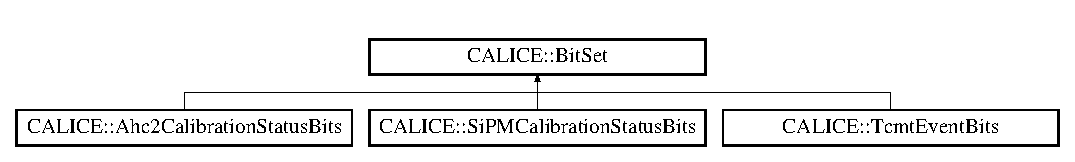
\includegraphics[height=1.728395cm]{classCALICE_1_1BitSet}
\end{center}
\end{figure}
\subsection*{Public Member Functions}
\begin{DoxyCompactItemize}
\item 
int {\bf get\-Int} () const 
\begin{DoxyCompactList}\small\item\em get integer corresponding to the bits \end{DoxyCompactList}\item 
void {\bf set\-Bits} (const int value)
\begin{DoxyCompactList}\small\item\em set all bits with an integer \end{DoxyCompactList}\item 
std\-::vector$<$ int $>$ {\bf get\-Int\-Vec} () const 
\begin{DoxyCompactList}\small\item\em get vector of ints with elements corresponding to the single bits (1 for true and 0 for false) \end{DoxyCompactList}\item 
void {\bf clear} ()\label{classCALICE_1_1BitSet_abd6be6d671e597c9c04afd73d25f7b6a}

\begin{DoxyCompactList}\small\item\em clear all bits to 0 \end{DoxyCompactList}\end{DoxyCompactItemize}
\subsection*{Protected Member Functions}
\begin{DoxyCompactItemize}
\item 
{\bf Bit\-Set} (const unsigned int max\-Bits, const int value=0x0)
\begin{DoxyCompactList}\small\item\em constructur \end{DoxyCompactList}\item 
bool {\bf get\-Bit} (unsigned int bit\-No) const 
\begin{DoxyCompactList}\small\item\em get function for bit number \end{DoxyCompactList}\item 
void {\bf set\-Bit} (unsigned int bit\-No, bool state)
\begin{DoxyCompactList}\small\item\em set function for bit number \end{DoxyCompactList}\end{DoxyCompactItemize}
\subsection*{Private Attributes}
\begin{DoxyCompactItemize}
\item 
int {\bfseries \-\_\-bits}\label{classCALICE_1_1BitSet_acb489ad5309a1343dc9d368fbfabb4e7}

\item 
unsigned int {\bfseries \-\_\-max\-Bits}\label{classCALICE_1_1BitSet_a0105ecaa0c1f03c666f90f3d3b7207c6}

\end{DoxyCompactItemize}


\subsection{Detailed Description}
Base class for easy definition of bit sets. 

Derived classes have to define the meaning of the bits. No instantiation possible.

\begin{DoxyAuthor}{Author}
{\tt Benjamin.\-Lutz@desy.\-de} 
\end{DoxyAuthor}
\begin{DoxyDate}{Date}
November 2009 
\end{DoxyDate}
\begin{DoxyVersion}{Version}
1.\-0 
\end{DoxyVersion}


Definition at line 18 of file Bit\-Set.\-hh.



\subsection{Constructor \& Destructor Documentation}
\index{C\-A\-L\-I\-C\-E\-::\-Bit\-Set@{C\-A\-L\-I\-C\-E\-::\-Bit\-Set}!Bit\-Set@{Bit\-Set}}
\index{Bit\-Set@{Bit\-Set}!CALICE::BitSet@{C\-A\-L\-I\-C\-E\-::\-Bit\-Set}}
\subsubsection[{Bit\-Set}]{\setlength{\rightskip}{0pt plus 5cm}C\-A\-L\-I\-C\-E\-::\-Bit\-Set\-::\-Bit\-Set (
\begin{DoxyParamCaption}
\item[{const unsigned int}]{max\-Bits, }
\item[{const int}]{value = {\ttfamily 0x0}}
\end{DoxyParamCaption}
)\hspace{0.3cm}{\ttfamily [inline]}, {\ttfamily [protected]}}\label{classCALICE_1_1BitSet_a73f400c579b2731fc366faf7fa873aa9}


constructur 

maximum number of bits defines the size of the returned vector


\begin{DoxyParams}[1]{Parameters}
\mbox{\tt in}  & {\em max\-Bits} & maximum number of bits \\
\hline
\mbox{\tt in}  & {\em value} & to initialise to different than 0 \\
\hline
\end{DoxyParams}


Definition at line 69 of file Bit\-Set.\-hh.



\subsection{Member Function Documentation}
\index{C\-A\-L\-I\-C\-E\-::\-Bit\-Set@{C\-A\-L\-I\-C\-E\-::\-Bit\-Set}!get\-Bit@{get\-Bit}}
\index{get\-Bit@{get\-Bit}!CALICE::BitSet@{C\-A\-L\-I\-C\-E\-::\-Bit\-Set}}
\subsubsection[{get\-Bit}]{\setlength{\rightskip}{0pt plus 5cm}bool C\-A\-L\-I\-C\-E\-::\-Bit\-Set\-::get\-Bit (
\begin{DoxyParamCaption}
\item[{unsigned int}]{bit\-No}
\end{DoxyParamCaption}
) const\hspace{0.3cm}{\ttfamily [inline]}, {\ttfamily [protected]}}\label{classCALICE_1_1BitSet_a0ffe3a5bdb4f4f5ec069c4330fef672b}


get function for bit number 


\begin{DoxyParams}{Parameters}
{\em bit\-No} & number of the bit to return \\
\hline
\end{DoxyParams}
\begin{DoxyReturn}{Returns}
state of bit 
\end{DoxyReturn}


Definition at line 80 of file Bit\-Set.\-hh.



Referenced by get\-Int\-Vec(), C\-A\-L\-I\-C\-E\-::\-Tcmt\-Event\-Bits\-::has\-Max\-Number\-Hits\-Muon(), C\-A\-L\-I\-C\-E\-::\-Tcmt\-Event\-Bits\-::has\-Max\-Number\-Muon\-Like\-Towers(), C\-A\-L\-I\-C\-E\-::\-Tcmt\-Event\-Bits\-::has\-Max\-Sum\-Energy\-Muon(), C\-A\-L\-I\-C\-E\-::\-Tcmt\-Event\-Bits\-::has\-Min\-Number\-Hits\-Muon(), C\-A\-L\-I\-C\-E\-::\-Tcmt\-Event\-Bits\-::has\-Min\-Number\-Muon\-Like\-Layers(), C\-A\-L\-I\-C\-E\-::\-Tcmt\-Event\-Bits\-::has\-Min\-Number\-Muon\-Like\-Towers(), C\-A\-L\-I\-C\-E\-::\-Tcmt\-Event\-Bits\-::has\-Min\-Sum\-Energy\-Muon(), C\-A\-L\-I\-C\-E\-::\-Tcmt\-Event\-Bits\-::is\-Leakage(), C\-A\-L\-I\-C\-E\-::\-Tcmt\-Event\-Bits\-::is\-Muon(), and C\-A\-L\-I\-C\-E\-::\-Tcmt\-Event\-Bits\-::is\-Pedestal().

\index{C\-A\-L\-I\-C\-E\-::\-Bit\-Set@{C\-A\-L\-I\-C\-E\-::\-Bit\-Set}!get\-Int@{get\-Int}}
\index{get\-Int@{get\-Int}!CALICE::BitSet@{C\-A\-L\-I\-C\-E\-::\-Bit\-Set}}
\subsubsection[{get\-Int}]{\setlength{\rightskip}{0pt plus 5cm}int C\-A\-L\-I\-C\-E\-::\-Bit\-Set\-::get\-Int (
\begin{DoxyParamCaption}
{}
\end{DoxyParamCaption}
) const\hspace{0.3cm}{\ttfamily [inline]}}\label{classCALICE_1_1BitSet_a148efced5e1ce099391216e2f4c9718a}


get integer corresponding to the bits 

\begin{DoxyReturn}{Returns}
integer with the bits set 
\end{DoxyReturn}


Definition at line 27 of file Bit\-Set.\-hh.



Referenced by C\-A\-L\-I\-C\-E\-::\-Tcmt\-Event\-Identifier\-::add\-Results().

\index{C\-A\-L\-I\-C\-E\-::\-Bit\-Set@{C\-A\-L\-I\-C\-E\-::\-Bit\-Set}!get\-Int\-Vec@{get\-Int\-Vec}}
\index{get\-Int\-Vec@{get\-Int\-Vec}!CALICE::BitSet@{C\-A\-L\-I\-C\-E\-::\-Bit\-Set}}
\subsubsection[{get\-Int\-Vec}]{\setlength{\rightskip}{0pt plus 5cm}std\-::vector$<$int$>$ C\-A\-L\-I\-C\-E\-::\-Bit\-Set\-::get\-Int\-Vec (
\begin{DoxyParamCaption}
{}
\end{DoxyParamCaption}
) const\hspace{0.3cm}{\ttfamily [inline]}}\label{classCALICE_1_1BitSet_a807161095aee85a74b6f520f32690ace}


get vector of ints with elements corresponding to the single bits (1 for true and 0 for false) 

\begin{DoxyReturn}{Returns}
vector of integers of single bits 
\end{DoxyReturn}


Definition at line 44 of file Bit\-Set.\-hh.



References get\-Bit().



Referenced by C\-A\-L\-I\-C\-E\-::\-Tcmt\-Event\-Identifier\-::add\-Results().

\index{C\-A\-L\-I\-C\-E\-::\-Bit\-Set@{C\-A\-L\-I\-C\-E\-::\-Bit\-Set}!set\-Bit@{set\-Bit}}
\index{set\-Bit@{set\-Bit}!CALICE::BitSet@{C\-A\-L\-I\-C\-E\-::\-Bit\-Set}}
\subsubsection[{set\-Bit}]{\setlength{\rightskip}{0pt plus 5cm}void C\-A\-L\-I\-C\-E\-::\-Bit\-Set\-::set\-Bit (
\begin{DoxyParamCaption}
\item[{unsigned int}]{bit\-No, }
\item[{bool}]{state}
\end{DoxyParamCaption}
)\hspace{0.3cm}{\ttfamily [inline]}, {\ttfamily [protected]}}\label{classCALICE_1_1BitSet_ae1b313a2e4a97fd9f197239f4abb9a49}


set function for bit number 


\begin{DoxyParams}{Parameters}
{\em bit\-No} & number of the bit to set \\
\hline
{\em state} & state to witch the bit gets set \\
\hline
\end{DoxyParams}


Definition at line 87 of file Bit\-Set.\-hh.

\index{C\-A\-L\-I\-C\-E\-::\-Bit\-Set@{C\-A\-L\-I\-C\-E\-::\-Bit\-Set}!set\-Bits@{set\-Bits}}
\index{set\-Bits@{set\-Bits}!CALICE::BitSet@{C\-A\-L\-I\-C\-E\-::\-Bit\-Set}}
\subsubsection[{set\-Bits}]{\setlength{\rightskip}{0pt plus 5cm}void C\-A\-L\-I\-C\-E\-::\-Bit\-Set\-::set\-Bits (
\begin{DoxyParamCaption}
\item[{const int}]{value}
\end{DoxyParamCaption}
)\hspace{0.3cm}{\ttfamily [inline]}}\label{classCALICE_1_1BitSet_a17ed04fb84b1be0b476312d046333704}


set all bits with an integer 


\begin{DoxyParams}[1]{Parameters}
\mbox{\tt in}  & {\em value} & integer with the bits \\
\hline
\end{DoxyParams}


Definition at line 34 of file Bit\-Set.\-hh.



The documentation for this class was generated from the following file\-:\begin{DoxyCompactItemize}
\item 
Bit\-Set.\-hh\end{DoxyCompactItemize}

\section{C\-A\-L\-I\-C\-E\-:\-:Bml\-Caen1290\-Configuration\-Block Class Reference}
\label{classCALICE_1_1BmlCaen1290ConfigurationBlock}\index{C\-A\-L\-I\-C\-E\-::\-Bml\-Caen1290\-Configuration\-Block@{C\-A\-L\-I\-C\-E\-::\-Bml\-Caen1290\-Configuration\-Block}}
Inheritance diagram for C\-A\-L\-I\-C\-E\-:\-:Bml\-Caen1290\-Configuration\-Block\-:\begin{figure}[H]
\begin{center}
\leavevmode
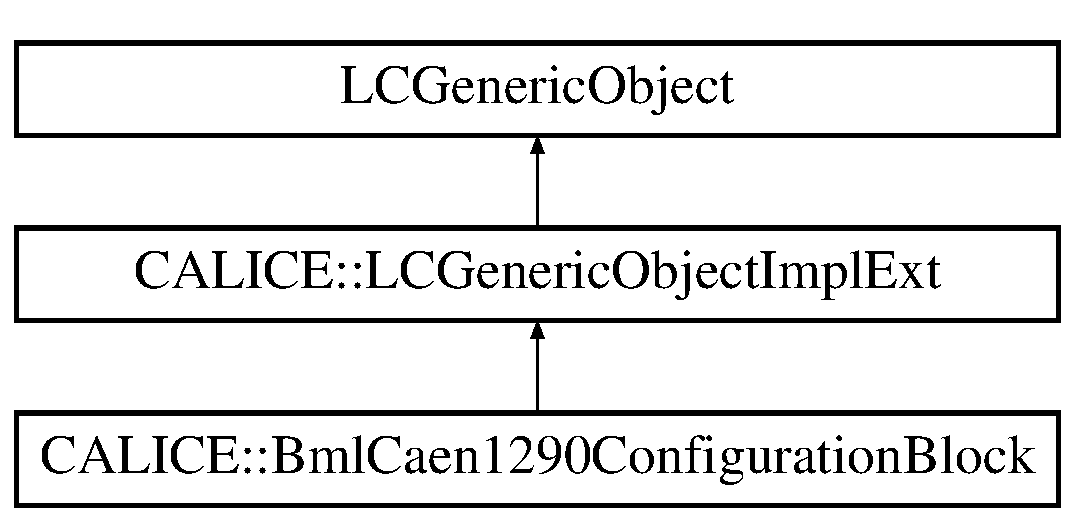
\includegraphics[height=3.000000cm]{classCALICE_1_1BmlCaen1290ConfigurationBlock}
\end{center}
\end{figure}
\subsection*{Public Member Functions}
\begin{DoxyCompactItemize}
\item 
{\bfseries Bml\-Caen1290\-Configuration\-Block} (L\-C\-Object $\ast${\bf obj})\label{classCALICE_1_1BmlCaen1290ConfigurationBlock_a2d4ea6c8b939a48a1236a7d38087a469}

\item 
{\bf Bml\-Caen1290\-Configuration\-Block} \& {\bfseries set\-Board\-I\-D} (int boardid)\label{classCALICE_1_1BmlCaen1290ConfigurationBlock_a26eb94a1bcb0960c8c36a8183e88fb7b}

\item 
int {\bfseries get\-Board\-I\-D} ()\label{classCALICE_1_1BmlCaen1290ConfigurationBlock_a7388b9a32d541f9f810e618e4e0090a6}

\item 
{\bf Bml\-Caen1290\-Configuration\-Block} \& {\bfseries set\-Base\-Address} (int baseaddress)\label{classCALICE_1_1BmlCaen1290ConfigurationBlock_a91ac6d8a2c5ed25692fd031b032286d8}

\item 
short {\bfseries get\-Base\-Address} () const \label{classCALICE_1_1BmlCaen1290ConfigurationBlock_aa3350ed9c44286ce22dadefa15a3f2b9}

\item 
{\bf Bml\-Caen1290\-Configuration\-Block} \& {\bfseries set\-Record\-Label} (int label)\label{classCALICE_1_1BmlCaen1290ConfigurationBlock_aa352775bfd0fefd8f159007a848680c7}

\item 
short {\bfseries get\-Record\-Label} () const \label{classCALICE_1_1BmlCaen1290ConfigurationBlock_aba8ba99a96410f121cbfe9ae0a0712c6}

\item 
{\bf Bml\-Caen1290\-Configuration\-Block} \& {\bfseries set\-Control\-Register} (int controlregister)\label{classCALICE_1_1BmlCaen1290ConfigurationBlock_aac6dd9b7a93bbe7018580d7ed2541994}

\item 
int {\bfseries get\-Control\-Register} ()\label{classCALICE_1_1BmlCaen1290ConfigurationBlock_a44e50c75db94105d7a558450b99b2d5a}

\item 
{\bf Bml\-Caen1290\-Configuration\-Block} \& {\bfseries set\-Interrupt\-Register} (int interruptregister)\label{classCALICE_1_1BmlCaen1290ConfigurationBlock_a81599fbfb68917487f0c62b74022fd11}

\item 
int {\bfseries get\-Interrupt\-Register} ()\label{classCALICE_1_1BmlCaen1290ConfigurationBlock_aaee03cf540e2494f17dc7837f32137d0}

\item 
{\bf Bml\-Caen1290\-Configuration\-Block} \& {\bfseries set\-Count\-Register} (int countregister)\label{classCALICE_1_1BmlCaen1290ConfigurationBlock_a457aedeb41da454148865f66f82c1ba4}

\item 
int {\bfseries get\-Count\-Register} ()\label{classCALICE_1_1BmlCaen1290ConfigurationBlock_a0c3d644ba875e29f3ce31fb0da51941f}

\item 
void {\bfseries print} (std\-::ostream \&os)\label{classCALICE_1_1BmlCaen1290ConfigurationBlock_adbb29adf8d9fd7ecd6e7176ac4348e13}

\item 
const std\-::string {\bfseries get\-Type\-Name} () const \label{classCALICE_1_1BmlCaen1290ConfigurationBlock_a1c568fad015045482af859b6432b1838}

\item 
const std\-::string {\bfseries get\-Data\-Description} () const \label{classCALICE_1_1BmlCaen1290ConfigurationBlock_a20a49557bcb139b1047748ce0cbd809a}

\end{DoxyCompactItemize}
\subsection*{Additional Inherited Members}


\subsection{Detailed Description}


Definition at line 22 of file Bml\-Caen1290\-Configuration\-Block.\-hh.



The documentation for this class was generated from the following file\-:\begin{DoxyCompactItemize}
\item 
Bml\-Caen1290\-Configuration\-Block.\-hh\end{DoxyCompactItemize}

\section{C\-A\-L\-I\-C\-E\-:\-:Bml\-Caen767\-Configuration\-Block Class Reference}
\label{classCALICE_1_1BmlCaen767ConfigurationBlock}\index{C\-A\-L\-I\-C\-E\-::\-Bml\-Caen767\-Configuration\-Block@{C\-A\-L\-I\-C\-E\-::\-Bml\-Caen767\-Configuration\-Block}}


Class to store configuration data of the 767 Caen T\-D\-C obsolete as of 31/10/10, replaced by \doxyref{Bml\-Caen\-Configuration\-Block}{p.}{classCALICE_1_1BmlCaenConfigurationBlock}, kept for backward compatibility of the code.  




{\ttfamily \#include $<$Bml\-Caen767\-Configuration\-Block.\-hh$>$}

Inheritance diagram for C\-A\-L\-I\-C\-E\-:\-:Bml\-Caen767\-Configuration\-Block\-:\begin{figure}[H]
\begin{center}
\leavevmode
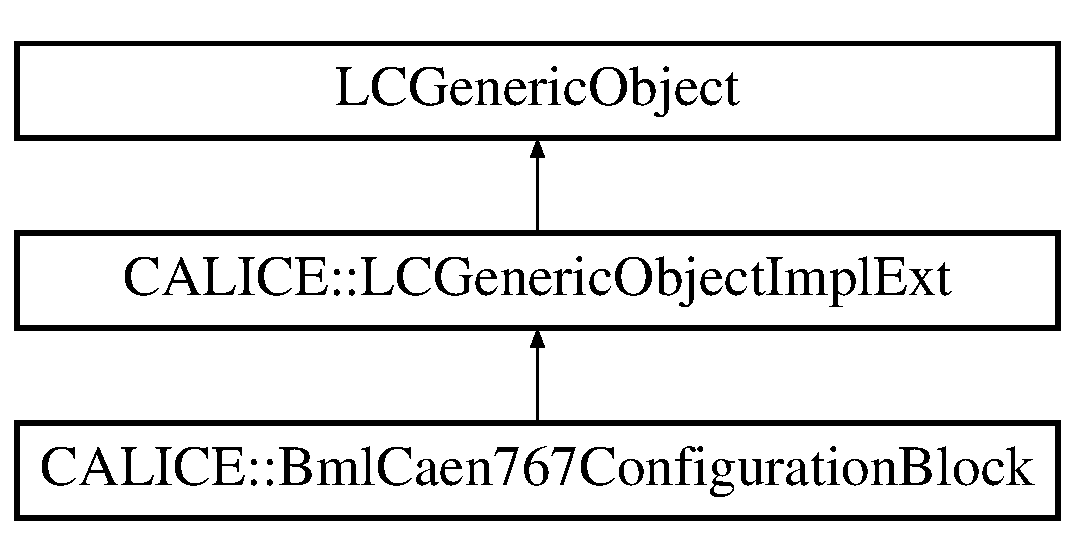
\includegraphics[height=3.000000cm]{classCALICE_1_1BmlCaen767ConfigurationBlock}
\end{center}
\end{figure}
\subsection*{Public Member Functions}
\begin{DoxyCompactItemize}
\item 
{\bfseries Bml\-Caen767\-Configuration\-Block} (L\-C\-Object $\ast${\bf obj})\label{classCALICE_1_1BmlCaen767ConfigurationBlock_a9d74204e08b6b2b3f8af2e33594bc427}

\item 
{\bf Bml\-Caen767\-Configuration\-Block} \& {\bfseries set\-Board\-I\-D} (int boardid)\label{classCALICE_1_1BmlCaen767ConfigurationBlock_a45d5e9f1b6b625e98498fe44e4e84b99}

\item 
int {\bfseries get\-Board\-I\-D} ()\label{classCALICE_1_1BmlCaen767ConfigurationBlock_aa5ed1065d3621938708124ad46ed42cd}

\item 
{\bf Bml\-Caen767\-Configuration\-Block} \& {\bfseries set\-Base\-Address} (int baseaddress)\label{classCALICE_1_1BmlCaen767ConfigurationBlock_af82dcd49f43b478d53d1817a84b72172}

\item 
short {\bfseries get\-Base\-Address} () const \label{classCALICE_1_1BmlCaen767ConfigurationBlock_a0afa51af661dd59e966b3d9853bd5815}

\item 
{\bf Bml\-Caen767\-Configuration\-Block} \& {\bfseries set\-Record\-Label} (int label)\label{classCALICE_1_1BmlCaen767ConfigurationBlock_a3c823c83fcfcc31b97c6841623144fa7}

\item 
short {\bfseries get\-Record\-Label} () const \label{classCALICE_1_1BmlCaen767ConfigurationBlock_a1e217f2e31b14e11233816c28a5a31e8}

\item 
{\bf Bml\-Caen767\-Configuration\-Block} \& {\bfseries set\-Control\-Register} (int controlregister)\label{classCALICE_1_1BmlCaen767ConfigurationBlock_aa04af84d56b57a3fbbd773b634515ba8}

\item 
int {\bfseries get\-Control\-Register} ()\label{classCALICE_1_1BmlCaen767ConfigurationBlock_a4ca9caf9f38105f5ae42ebb26e14949d}

\item 
{\bf Bml\-Caen767\-Configuration\-Block} \& {\bfseries set\-Interrupt\-Register} (int interruptregister)\label{classCALICE_1_1BmlCaen767ConfigurationBlock_ac915c9120ba54f8a499a09ba97b55c70}

\item 
int {\bfseries get\-Interrupt\-Register} ()\label{classCALICE_1_1BmlCaen767ConfigurationBlock_a24a4cc23e5d53f80a349c6fc75609e13}

\item 
void {\bfseries print} (std\-::ostream \&os)\label{classCALICE_1_1BmlCaen767ConfigurationBlock_a0187bcd935e12e88d5fadbae84fdb224}

\item 
const std\-::string {\bfseries get\-Type\-Name} () const \label{classCALICE_1_1BmlCaen767ConfigurationBlock_aeb8004b87f36dda36e7c713f38e618b5}

\item 
const std\-::string {\bfseries get\-Data\-Description} () const \label{classCALICE_1_1BmlCaen767ConfigurationBlock_aea6f25e18e5758e6c82df338b13d05a1}

\end{DoxyCompactItemize}
\subsection*{Additional Inherited Members}


\subsection{Detailed Description}
Class to store configuration data of the 767 Caen T\-D\-C obsolete as of 31/10/10, replaced by \doxyref{Bml\-Caen\-Configuration\-Block}{p.}{classCALICE_1_1BmlCaenConfigurationBlock}, kept for backward compatibility of the code. 

\begin{DoxyAuthor}{Author}
R.\-Poeschl (L\-A\-L Orsay) 
\end{DoxyAuthor}
\begin{DoxyDate}{Date}
Aug 01 2006 
\end{DoxyDate}


Definition at line 30 of file Bml\-Caen767\-Configuration\-Block.\-hh.



The documentation for this class was generated from the following file\-:\begin{DoxyCompactItemize}
\item 
Bml\-Caen767\-Configuration\-Block.\-hh\end{DoxyCompactItemize}

\section{C\-A\-L\-I\-C\-E\-:\-:Bml\-Caen767\-Readout\-Configuration\-Block Class Reference}
\label{classCALICE_1_1BmlCaen767ReadoutConfigurationBlock}\index{C\-A\-L\-I\-C\-E\-::\-Bml\-Caen767\-Readout\-Configuration\-Block@{C\-A\-L\-I\-C\-E\-::\-Bml\-Caen767\-Readout\-Configuration\-Block}}


Stores the configuration of the Caen767 T\-D\-C into the database At the moment I am writing this class I don't know whether they'll serve for something but it is a small uncomplicated class, so here we go.  




{\ttfamily \#include $<$Bml\-Caen767\-Readout\-Configuration\-Block.\-hh$>$}

Inheritance diagram for C\-A\-L\-I\-C\-E\-:\-:Bml\-Caen767\-Readout\-Configuration\-Block\-:\begin{figure}[H]
\begin{center}
\leavevmode
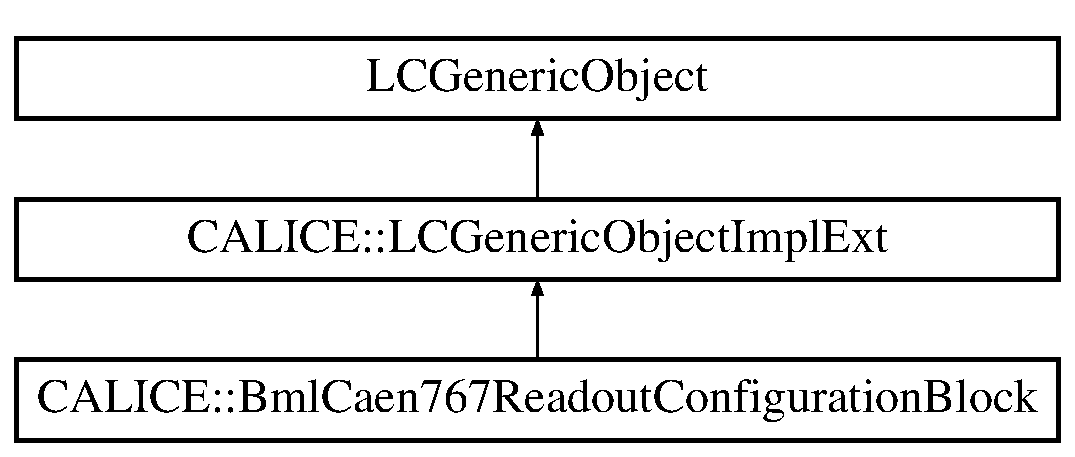
\includegraphics[height=3.000000cm]{classCALICE_1_1BmlCaen767ReadoutConfigurationBlock}
\end{center}
\end{figure}
\subsection*{Public Member Functions}
\begin{DoxyCompactItemize}
\item 
{\bf Bml\-Caen767\-Readout\-Configuration\-Block} ()\label{classCALICE_1_1BmlCaen767ReadoutConfigurationBlock_a7b9ac595633452fbbdee1892e94773a2}

\begin{DoxyCompactList}\small\item\em Default Constructor. \end{DoxyCompactList}\item 
{\bf Bml\-Caen767\-Readout\-Configuration\-Block} (L\-C\-Object $\ast${\bf obj})\label{classCALICE_1_1BmlCaen767ReadoutConfigurationBlock_aee0f6722067d06d4583bea18ffb2dc1e}

\begin{DoxyCompactList}\small\item\em 'Copy constructor' needed to interpret L\-C\-Collection read from file/database. \end{DoxyCompactList}\item 
{\bf Bml\-Caen767\-Readout\-Configuration\-Block} \& {\bf set\-Crate\-Number} (int cratenumber)
\begin{DoxyCompactList}\small\item\em set the packed board id. \end{DoxyCompactList}\item 
int {\bf get\-Crate\-Number} ()\label{classCALICE_1_1BmlCaen767ReadoutConfigurationBlock_a98283f15edae4729e382eaa0ef556be4}

\begin{DoxyCompactList}\small\item\em Return the crate number. \end{DoxyCompactList}\item 
{\bf Bml\-Caen767\-Readout\-Configuration\-Block} \& {\bf set\-Read\-Period} (int readperiod)\label{classCALICE_1_1BmlCaen767ReadoutConfigurationBlock_ad7910acd3e581a551f968402cb943a5d}

\begin{DoxyCompactList}\small\item\em Set the Read Period. \end{DoxyCompactList}\item 
unsigned int {\bf get\-Read\-Period} () const \label{classCALICE_1_1BmlCaen767ReadoutConfigurationBlock_a55139c919133134fc95514a97252c99b}

\begin{DoxyCompactList}\small\item\em Return the Read Period. \end{DoxyCompactList}\item 
{\bf Bml\-Caen767\-Readout\-Configuration\-Block} \& {\bf set\-Bools} (bool enable, bool softtrigger, bool bltro, bool arrayro)\label{classCALICE_1_1BmlCaen767ReadoutConfigurationBlock_a0f4e57ffa62de58619397cdc8b203f42}

\begin{DoxyCompactList}\small\item\em Store the indicators of the readout mode. \end{DoxyCompactList}\item 
bool {\bfseries is\-Enabled} ()\label{classCALICE_1_1BmlCaen767ReadoutConfigurationBlock_a6a822edd1400153f4db0d779fa24862b}

\item 
bool {\bfseries is\-Soft\-Trigger} ()\label{classCALICE_1_1BmlCaen767ReadoutConfigurationBlock_ae6a1be49e52e35b4966ebc0c373bcdff}

\item 
bool {\bfseries is\-Blt\-Readout} ()\label{classCALICE_1_1BmlCaen767ReadoutConfigurationBlock_a9aad9174d74e8f233e456c807f28ec97}

\item 
bool {\bfseries is\-Array\-Readout} ()\label{classCALICE_1_1BmlCaen767ReadoutConfigurationBlock_ad67e67c908f7f4a337c9d2ea61a93229}

\item 
{\bf Bml\-Caen767\-Readout\-Configuration\-Block} \& {\bf set\-Mode} (int mode)
\begin{DoxyCompactList}\small\item\em Store the readout mode word note that this word contains the information which you also get with the is\-Soft\-Trigger, is\-Enable, get\-Crate\-Number etc. \end{DoxyCompactList}\item 
int {\bf get\-Mode} ()\label{classCALICE_1_1BmlCaen767ReadoutConfigurationBlock_a317aceac7a964643ece66c7f280ed79b}

\begin{DoxyCompactList}\small\item\em Return the readout mode word. \end{DoxyCompactList}\item 
void {\bf print} (std\-::ostream \&os)\label{classCALICE_1_1BmlCaen767ReadoutConfigurationBlock_a2abf8314fda5aab33b4d3bee730f3c77}

\begin{DoxyCompactList}\small\item\em Convenient print method. \end{DoxyCompactList}\item 
const std\-::string {\bf get\-Type\-Name} () const \label{classCALICE_1_1BmlCaen767ReadoutConfigurationBlock_a72df8e4c6c2ea5a90fe48efe92844010}

\begin{DoxyCompactList}\small\item\em Return the type of the class. \end{DoxyCompactList}\item 
const std\-::string {\bf get\-Data\-Description} () const \label{classCALICE_1_1BmlCaen767ReadoutConfigurationBlock_a8adf9e63470589b2e516edf3642d297e}

\begin{DoxyCompactList}\small\item\em Return a brief description of the data members. \end{DoxyCompactList}\end{DoxyCompactItemize}
\subsection*{Additional Inherited Members}


\subsection{Detailed Description}
Stores the configuration of the Caen767 T\-D\-C into the database At the moment I am writing this class I don't know whether they'll serve for something but it is a small uncomplicated class, so here we go. 

\begin{DoxySeeAlso}{See Also}
\doxyref{Conditions\-Change\-Delegator}{p.}{classCALICE_1_1ConditionsChangeDelegator} 
\end{DoxySeeAlso}
\begin{DoxyAuthor}{Author}
R. Poeschl L\-A\-L (based on the other interface classes)
\end{DoxyAuthor}
\begin{DoxyDate}{Date}
Aug 2006 
\end{DoxyDate}


Definition at line 36 of file Bml\-Caen767\-Readout\-Configuration\-Block.\-hh.



\subsection{Member Function Documentation}
\index{C\-A\-L\-I\-C\-E\-::\-Bml\-Caen767\-Readout\-Configuration\-Block@{C\-A\-L\-I\-C\-E\-::\-Bml\-Caen767\-Readout\-Configuration\-Block}!set\-Crate\-Number@{set\-Crate\-Number}}
\index{set\-Crate\-Number@{set\-Crate\-Number}!CALICE::BmlCaen767ReadoutConfigurationBlock@{C\-A\-L\-I\-C\-E\-::\-Bml\-Caen767\-Readout\-Configuration\-Block}}
\subsubsection[{set\-Crate\-Number}]{\setlength{\rightskip}{0pt plus 5cm}{\bf Bml\-Caen767\-Readout\-Configuration\-Block}\& C\-A\-L\-I\-C\-E\-::\-Bml\-Caen767\-Readout\-Configuration\-Block\-::set\-Crate\-Number (
\begin{DoxyParamCaption}
\item[{int}]{cratenumber}
\end{DoxyParamCaption}
)\hspace{0.3cm}{\ttfamily [inline]}}\label{classCALICE_1_1BmlCaen767ReadoutConfigurationBlock_ae18446e9805a9701e97a7153f9f139ce}


set the packed board id. 

\begin{DoxySeeAlso}{See Also}
\doxyref{Board\-I\-D}{p.}{classCALICE_1_1BoardID} For the Caen 767 T\-D\-C the board\-I\-D has a slightly different meaning compared with the Crc\-Boards slot\-I\-D and board component numbers are just the M\-S\-B and L\-S\-B of the base address.\-Set the crate number 
\end{DoxySeeAlso}


Definition at line 60 of file Bml\-Caen767\-Readout\-Configuration\-Block.\-hh.

\index{C\-A\-L\-I\-C\-E\-::\-Bml\-Caen767\-Readout\-Configuration\-Block@{C\-A\-L\-I\-C\-E\-::\-Bml\-Caen767\-Readout\-Configuration\-Block}!set\-Mode@{set\-Mode}}
\index{set\-Mode@{set\-Mode}!CALICE::BmlCaen767ReadoutConfigurationBlock@{C\-A\-L\-I\-C\-E\-::\-Bml\-Caen767\-Readout\-Configuration\-Block}}
\subsubsection[{set\-Mode}]{\setlength{\rightskip}{0pt plus 5cm}{\bf Bml\-Caen767\-Readout\-Configuration\-Block}\& C\-A\-L\-I\-C\-E\-::\-Bml\-Caen767\-Readout\-Configuration\-Block\-::set\-Mode (
\begin{DoxyParamCaption}
\item[{int}]{mode}
\end{DoxyParamCaption}
)\hspace{0.3cm}{\ttfamily [inline]}}\label{classCALICE_1_1BmlCaen767ReadoutConfigurationBlock_a73230994b130b114873b2f9b87f7fb25}


Store the readout mode word note that this word contains the information which you also get with the is\-Soft\-Trigger, is\-Enable, get\-Crate\-Number etc. 

methods we add the word in case meaning of the bits therein have changed or new inidcators are added and we weren't aware of it. Hence this is just a safety net 

Definition at line 116 of file Bml\-Caen767\-Readout\-Configuration\-Block.\-hh.



The documentation for this class was generated from the following file\-:\begin{DoxyCompactItemize}
\item 
Bml\-Caen767\-Readout\-Configuration\-Block.\-hh\end{DoxyCompactItemize}

\section{C\-A\-L\-I\-C\-E\-:\-:Bml\-Caen\-Configuration\-Block Class Reference}
\label{classCALICE_1_1BmlCaenConfigurationBlock}\index{C\-A\-L\-I\-C\-E\-::\-Bml\-Caen\-Configuration\-Block@{C\-A\-L\-I\-C\-E\-::\-Bml\-Caen\-Configuration\-Block}}


Class to store configuration data of the Caen T\-D\-Cs (767, 1290) Replaces Bml\-Caen767\-Configuration\-Data.  




{\ttfamily \#include $<$Bml\-Caen\-Configuration\-Block.\-hh$>$}

Inheritance diagram for C\-A\-L\-I\-C\-E\-:\-:Bml\-Caen\-Configuration\-Block\-:\begin{figure}[H]
\begin{center}
\leavevmode
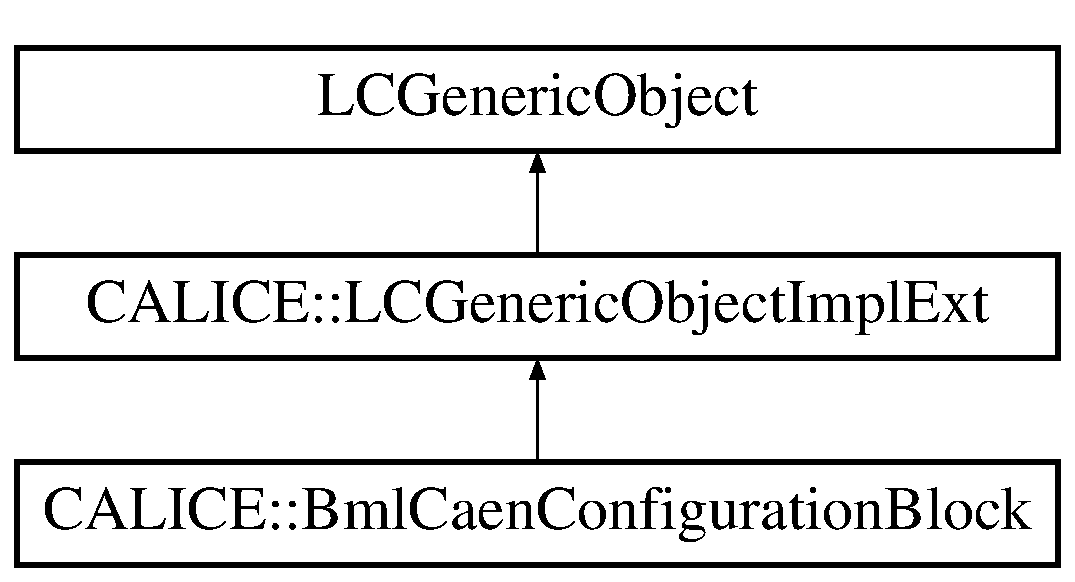
\includegraphics[height=3.000000cm]{classCALICE_1_1BmlCaenConfigurationBlock}
\end{center}
\end{figure}
\subsection*{Public Member Functions}
\begin{DoxyCompactItemize}
\item 
{\bfseries Bml\-Caen\-Configuration\-Block} (L\-C\-Object $\ast${\bf obj})\label{classCALICE_1_1BmlCaenConfigurationBlock_a15ef15c6db9d50ae58e65f2c98ed73bd}

\item 
{\bf Bml\-Caen\-Configuration\-Block} \& {\bfseries set\-Board\-I\-D} (int boardid)\label{classCALICE_1_1BmlCaenConfigurationBlock_a59fe78bec24532de95313aef863c9ff2}

\item 
int {\bfseries get\-Board\-I\-D} ()\label{classCALICE_1_1BmlCaenConfigurationBlock_a360a11a0204d58df71637193c4b9ead1}

\item 
{\bf Bml\-Caen\-Configuration\-Block} \& {\bfseries set\-Base\-Address} (int baseaddress)\label{classCALICE_1_1BmlCaenConfigurationBlock_a079fc5fd9026b0ef6c05fe33317290e9}

\item 
short {\bfseries get\-Base\-Address} () const \label{classCALICE_1_1BmlCaenConfigurationBlock_a8e7b031737715e85f55e8b4125d0b76b}

\item 
{\bf Bml\-Caen\-Configuration\-Block} \& {\bfseries set\-Record\-Label} (int label)\label{classCALICE_1_1BmlCaenConfigurationBlock_ac272a9c66fd223224a2a200cb7d2a66b}

\item 
short {\bfseries get\-Record\-Label} () const \label{classCALICE_1_1BmlCaenConfigurationBlock_aa8b83429f623d10f65edabe8a8b5a4a1}

\item 
{\bf Bml\-Caen\-Configuration\-Block} \& {\bfseries set\-Control\-Register} (int controlregister)\label{classCALICE_1_1BmlCaenConfigurationBlock_adf3f1a86fc1b8e1088669ae247dc96a6}

\item 
int {\bfseries get\-Control\-Register} ()\label{classCALICE_1_1BmlCaenConfigurationBlock_acbcca488fd13727aa889f6ad53c8f4dc}

\item 
{\bf Bml\-Caen\-Configuration\-Block} \& {\bfseries set\-Interrupt\-Register} (int interruptregister)\label{classCALICE_1_1BmlCaenConfigurationBlock_aebab0b05f74576366201b44bee1752a6}

\item 
int {\bfseries get\-Interrupt\-Register} ()\label{classCALICE_1_1BmlCaenConfigurationBlock_af4ee7799dca9ad03e3d214b1d736fa13}

\item 
{\bf Bml\-Caen\-Configuration\-Block} \& {\bfseries set\-Count\-Register} (int countregister)\label{classCALICE_1_1BmlCaenConfigurationBlock_a49de9d6d4578e37f78362ca9be910cae}

\item 
int {\bfseries get\-Count\-Register} ()\label{classCALICE_1_1BmlCaenConfigurationBlock_a4b63566dafbbe73c046ea94962f28c4d}

\item 
{\bf Bml\-Caen\-Configuration\-Block} \& {\bfseries set\-Spare} (int spare)\label{classCALICE_1_1BmlCaenConfigurationBlock_a25eafb2a9abb905b2fcea1395d735225}

\item 
int {\bfseries get\-Spare} ()\label{classCALICE_1_1BmlCaenConfigurationBlock_a56e1badfdaed4148f5c89c045a9d8e2f}

\item 
void {\bfseries print} (std\-::ostream \&os)\label{classCALICE_1_1BmlCaenConfigurationBlock_a68dbb32906d68303dad6b5f4a8ba35c2}

\item 
const std\-::string {\bfseries get\-Type\-Name} () const \label{classCALICE_1_1BmlCaenConfigurationBlock_ae6b54fef6a2a397b27237787b4c1ad24}

\item 
const std\-::string {\bfseries get\-Data\-Description} () const \label{classCALICE_1_1BmlCaenConfigurationBlock_a8bd06c4d35fb60d77e1bedb3a53a3523}

\end{DoxyCompactItemize}
\subsection*{Additional Inherited Members}


\subsection{Detailed Description}
Class to store configuration data of the Caen T\-D\-Cs (767, 1290) Replaces Bml\-Caen767\-Configuration\-Data. 

\begin{DoxyAuthor}{Author}
R.\-Poeschl (L\-A\-L Orsay) 
\end{DoxyAuthor}
\begin{DoxyDate}{Date}
Oct 31 2010 
\end{DoxyDate}


Definition at line 29 of file Bml\-Caen\-Configuration\-Block.\-hh.



The documentation for this class was generated from the following file\-:\begin{DoxyCompactItemize}
\item 
Bml\-Caen\-Configuration\-Block.\-hh\end{DoxyCompactItemize}

\section{C\-A\-L\-I\-C\-E\-:\-:Bml\-Event\-Data Class Reference}
\label{classCALICE_1_1BmlEventData}\index{C\-A\-L\-I\-C\-E\-::\-Bml\-Event\-Data@{C\-A\-L\-I\-C\-E\-::\-Bml\-Event\-Data}}


Class to store the \doxyref{Bml\-Event\-Data}{p.}{classCALICE_1_1BmlEventData}.  




{\ttfamily \#include $<$Bml\-Event\-Data.\-hh$>$}

Inheritance diagram for C\-A\-L\-I\-C\-E\-:\-:Bml\-Event\-Data\-:\begin{figure}[H]
\begin{center}
\leavevmode
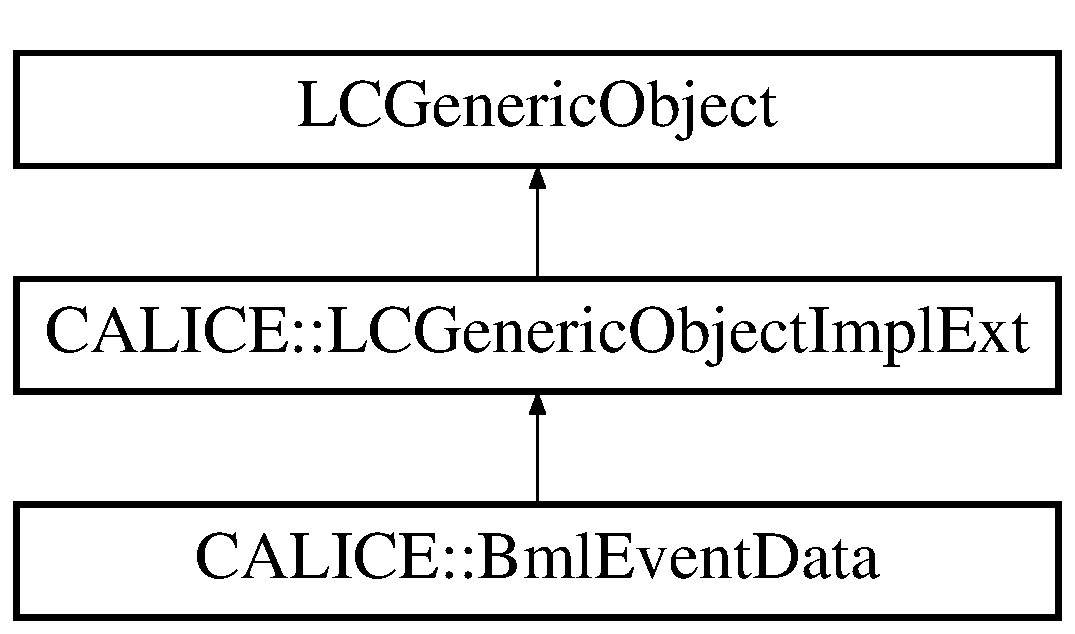
\includegraphics[height=3.000000cm]{classCALICE_1_1BmlEventData}
\end{center}
\end{figure}
\subsection*{Public Member Functions}
\begin{DoxyCompactItemize}
\item 
{\bf Bml\-Event\-Data} ()\label{classCALICE_1_1BmlEventData_aa67d8ecf7a32109b97c00cffd6ac68c3}

\begin{DoxyCompactList}\small\item\em Default Constructor. \end{DoxyCompactList}\item 
{\bf Bml\-Event\-Data} (L\-C\-Object $\ast${\bf obj})\label{classCALICE_1_1BmlEventData_a556af620c0b013022a16363eb93d72d6}

\begin{DoxyCompactList}\small\item\em A copy constructor. \end{DoxyCompactList}\item 
virtual {\bf $\sim$\-Bml\-Event\-Data} ()\label{classCALICE_1_1BmlEventData_a465574a0d2cb1c9cec3cc9e0e543f7ae}

\begin{DoxyCompactList}\small\item\em The destructor. \end{DoxyCompactList}\item 
void {\bf add\-Supplementary\-Information} (L\-C\-Event $\ast$a\-Evt, unsigned int ielm)
\begin{DoxyCompactList}\small\item\em Add supplementary information\-: Feed information not available in the actual \doxyref{Bml\-Event\-Data}{p.}{classCALICE_1_1BmlEventData} to the object. \end{DoxyCompactList}\item 
{\bf Bml\-Event\-Data} \& {\bf set\-Board\-I\-D} (int board\-I\-D)
\begin{DoxyCompactList}\small\item\em set the packed board id. \end{DoxyCompactList}\item 
int {\bf get\-Board\-I\-D} () const \label{classCALICE_1_1BmlEventData_a802624fa05776cd6430c6876ef65d950}

\begin{DoxyCompactList}\small\item\em get the board id \end{DoxyCompactList}\item 
{\bf Bml\-Event\-Data} \& {\bf set\-Base\-Address} (int baseaddress)\label{classCALICE_1_1BmlEventData_afea25a27f1395bb140196b87c311d4a4}

\begin{DoxyCompactList}\small\item\em Set the Base Address of this T\-D\-C. \end{DoxyCompactList}\item 
short {\bf get\-Base\-Address} () const \label{classCALICE_1_1BmlEventData_a392737613082f9752a2c5e84a45e3201}

\begin{DoxyCompactList}\small\item\em Return the Base Address. \end{DoxyCompactList}\item 
{\bf Bml\-Event\-Data} \& {\bf set\-Record\-Label} (int label)\label{classCALICE_1_1BmlEventData_acec730905f3fce6555d2f59fa5ba19cf}

\begin{DoxyCompactList}\small\item\em Set the Record Label. \end{DoxyCompactList}\item 
short {\bf get\-Record\-Label} () const \label{classCALICE_1_1BmlEventData_ae80cac54546f6f102f069414ed031c3d}

\begin{DoxyCompactList}\small\item\em Return the Record Label. \end{DoxyCompactList}\item 
{\bf Bml\-Event\-Data} \& {\bf set\-Status\-Register} (int statreg)\label{classCALICE_1_1BmlEventData_aefe41281cd9af82a4a24c08d2ab1269b}

\begin{DoxyCompactList}\small\item\em Set the status register Value. \end{DoxyCompactList}\item 
int {\bf get\-Status\-Register} () const \label{classCALICE_1_1BmlEventData_a35bc6ad106c13c03be291494e19904b0}

\begin{DoxyCompactList}\small\item\em Get the status register value. \end{DoxyCompactList}\item 
{\bf Bml\-Event\-Data} \& {\bf set\-Number\-Of\-Words} (int numwords)\label{classCALICE_1_1BmlEventData_a7aee8d1aad0f8fe7e2489362a17085be}

\begin{DoxyCompactList}\small\item\em Set the number of words. \end{DoxyCompactList}\item 
int {\bf get\-Number\-Of\-Words} () const \label{classCALICE_1_1BmlEventData_a62adde679450ee19364121aabe84b419}

\begin{DoxyCompactList}\small\item\em Get the number of words. \end{DoxyCompactList}\item 
{\bf Bml\-Event\-Data} \& {\bf set\-Geo\-Address} (int geoaddress)\label{classCALICE_1_1BmlEventData_a7932d1fb4d2ee46a8e99cd37967b2b4c}

\begin{DoxyCompactList}\small\item\em Set the geo Address of the T\-D\-C. \end{DoxyCompactList}\item 
int {\bf get\-Geo\-Address} () const \label{classCALICE_1_1BmlEventData_a10e6df6233068413112a80f2019aabc0}

\begin{DoxyCompactList}\small\item\em Get the geo Address. \end{DoxyCompactList}\item 
{\bf Bml\-Event\-Data} \& {\bf set\-Event\-Number} (int eventnumber)\label{classCALICE_1_1BmlEventData_a860cacaab0517981c00347d202237120}

\begin{DoxyCompactList}\small\item\em Set the event number as counted by the T\-D\-C. \end{DoxyCompactList}\item 
int {\bf get\-Event\-Number} () const \label{classCALICE_1_1BmlEventData_a82cf900eb42abb77da0a0e85c6a9968f}

\begin{DoxyCompactList}\small\item\em Get the event Number. \end{DoxyCompactList}\item 
{\bf Bml\-Event\-Data} \& {\bf set\-Status} (int status)\label{classCALICE_1_1BmlEventData_a9f65a78e21ff2816ba4fbe96ef240bd9}

\begin{DoxyCompactList}\small\item\em Set status as present when the the eob record appears. \end{DoxyCompactList}\item 
int {\bf get\-Status} () const \label{classCALICE_1_1BmlEventData_a30f49cce27697fb66ad59add06094e35}

\begin{DoxyCompactList}\small\item\em Get the status value. \end{DoxyCompactList}\item 
{\bf Bml\-Event\-Data} \& {\bf set\-Event\-Data\-Counter} (int evtdatacounter)\label{classCALICE_1_1BmlEventData_aabf7d25451c61875c4dde0f33a33f366}

\begin{DoxyCompactList}\small\item\em Set the Event\-Data counter as present when the the eob record appears. \end{DoxyCompactList}\item 
int {\bf get\-Event\-Data\-Counter} () const \label{classCALICE_1_1BmlEventData_a22685cc5c125541fd7dff408bf11a6ea}

\begin{DoxyCompactList}\small\item\em Get the event data counter value. \end{DoxyCompactList}\item 
int {\bf get\-Number\-Of\-Signal\-Channels} () const \label{classCALICE_1_1BmlEventData_a1142020abee10914560bf8eba80b6225}

\begin{DoxyCompactList}\small\item\em Get the number of channels which carry a signal. \end{DoxyCompactList}\item 
{\bf Bml\-Event\-Data} \& {\bf set\-T\-D\-C\-Type} (std\-::string type\-Str)
\begin{DoxyCompactList}\small\item\em Here follow the setting and getting of the information from the class holding supplementary information. \end{DoxyCompactList}\item 
std\-::string {\bf get\-T\-D\-C\-Type} ()\label{classCALICE_1_1BmlEventData_a816f61c11888b918a14dad1fc9301c7e}

\begin{DoxyCompactList}\small\item\em retrieve the typename \end{DoxyCompactList}\item 
{\bf Bml\-Event\-Data} \& {\bf set\-Event\-Fifo\-Cont} (int fifocont)
\begin{DoxyCompactList}\small\item\em set the Fifo Cont id. \end{DoxyCompactList}\item 
unsigned short {\bf get\-Word\-Count} ()\label{classCALICE_1_1BmlEventData_a2a65e16561e4df0b260561713e982c8d}

\begin{DoxyCompactList}\small\item\em get the word count \end{DoxyCompactList}\item 
unsigned short {\bf get\-Event\-Count} ()\label{classCALICE_1_1BmlEventData_af1fce77ca4743c7733dfe0952f960244}

\begin{DoxyCompactList}\small\item\em get the event count \end{DoxyCompactList}\item 
{\bf Bml\-Event\-Data} \& {\bf set\-Bunch\-I\-D} (int bunch\-I\-D)
\begin{DoxyCompactList}\small\item\em set the bunch id. \end{DoxyCompactList}\item 
unsigned int {\bf get\-Bunch\-I\-D} ()\label{classCALICE_1_1BmlEventData_a2768e6cfbde1495d057a6cd36e581a3b}

\begin{DoxyCompactList}\small\item\em get the bunch id \end{DoxyCompactList}\item 
{\bf Bml\-Event\-Data} \& {\bf set\-Event\-I\-D\-Trailer} (int event\-I\-D\-Trailer)\label{classCALICE_1_1BmlEventData_a527c6d1ba7a7e575f16dd95a5b5c198b}

\begin{DoxyCompactList}\small\item\em Set the eventid from the T\-D\-C trailer. \end{DoxyCompactList}\item 
unsigned int {\bf get\-Event\-I\-D\-Trailer} ()\label{classCALICE_1_1BmlEventData_a7e5b77a0457590fad53a5983ea7c7e7b}

\begin{DoxyCompactList}\small\item\em get the event id trailer \end{DoxyCompactList}\item 
{\bf Bml\-Event\-Data} \& {\bf set\-T\-D\-C\-Errors} (int tdc\-Errors)\label{classCALICE_1_1BmlEventData_a7d3195e0c08976bfc5e1122efea915cf}

\begin{DoxyCompactList}\small\item\em Set the T\-D\-C errors. \end{DoxyCompactList}\item 
unsigned int {\bf get\-T\-D\-C\-Errors} ()\label{classCALICE_1_1BmlEventData_a30e07f8dc96ecb2aadac9606dbf9b4f9}

\begin{DoxyCompactList}\small\item\em get the tdc errors \end{DoxyCompactList}\item 
{\bf Bml\-Event\-Data} \& {\bf set\-Buffer\-Overflow} (int buffer\-Overflow)\label{classCALICE_1_1BmlEventData_a03eecee3ea4ae146c3320caee9ba813f}

\begin{DoxyCompactList}\small\item\em Set the buffer overflow. \end{DoxyCompactList}\item 
unsigned int {\bf get\-Buffer\-Overflow} ()\label{classCALICE_1_1BmlEventData_a42a5c16c75f78d794441830c9eae1cb7}

\begin{DoxyCompactList}\small\item\em get the buffer overflow \end{DoxyCompactList}\item 
{\bf Bml\-Event\-Data} \& {\bf set\-Trigger\-Lost} (int triggerlost)\label{classCALICE_1_1BmlEventData_ae97639de2ca13acb95d0cbbef7d51b7a}

\begin{DoxyCompactList}\small\item\em Set the number of words in the trailer. \end{DoxyCompactList}\item 
unsigned int {\bf get\-Trigger\-Lost} ()\label{classCALICE_1_1BmlEventData_a1a250cc192a3874ca587efd9712bc27c}

\begin{DoxyCompactList}\small\item\em Get information on lost triggers. \end{DoxyCompactList}\item 
{\bf Bml\-Event\-Data} \& {\bf set\-T\-D\-C\-Word\-Count\-Trailer} (int numwords)\label{classCALICE_1_1BmlEventData_a37546da528d855946dfc12faa2a836d4}

\begin{DoxyCompactList}\small\item\em Set the number of words in the trailer. \end{DoxyCompactList}\item 
unsigned int {\bf get\-T\-D\-C\-Word\-Count\-Trailer} ()\label{classCALICE_1_1BmlEventData_a16022acb74c6d58f32ea5388a16ed752}

\begin{DoxyCompactList}\small\item\em Get the number of words in the trailer. \end{DoxyCompactList}\item 
{\bf Bml\-Event\-Data\-Sup} $\ast$ {\bf get\-Sup\-Object} ()\label{classCALICE_1_1BmlEventData_ab7a136495e35b3c0d9ce8e14052b7a38}

\begin{DoxyCompactList}\small\item\em return the supplementary object \end{DoxyCompactList}\item 
void {\bf add\-T\-D\-C\-Channels} (const T\-D\-C\-Channel\-Container\-\_\-t \&)
\begin{DoxyCompactList}\small\item\em Get measurements for each tdc channel The data are stored at the end of the collection with the following 'protocol' channelnumber number of signals m startime word, i.\-e. \end{DoxyCompactList}\item 
const T\-D\-C\-Channel\-Container\-\_\-t \& {\bf get\-T\-D\-C\-Channel\-Container} ()
\begin{DoxyCompactList}\small\item\em Returns a container with tdc channel info The first part of the map is the channelnumber The second part of the map is a pair consisting of an indicator whether the measurement is a starttime and the actual time measurement (the core of it all) falling egdes are indicated by a minus sign. \end{DoxyCompactList}\item 
const std\-::string {\bf get\-Type\-Name} () const \label{classCALICE_1_1BmlEventData_a7113442068c692c4a4734204006d1801}

\begin{DoxyCompactList}\small\item\em returns the the type name \end{DoxyCompactList}\item 
const std\-::string {\bf get\-Data\-Description} () const \label{classCALICE_1_1BmlEventData_ab525cda04a44662b1054fa7d52729e41}

\begin{DoxyCompactList}\small\item\em returns a brief description of the data stored \end{DoxyCompactList}\item 
std\-::ostream \& {\bf print} (std\-::ostream \&ostrm)\label{classCALICE_1_1BmlEventData_aef388c90f9b4060f6a14ae4c95cea7f8}

\begin{DoxyCompactList}\small\item\em dumps data content \end{DoxyCompactList}\item 
void {\bf print\-Init\-Warning} ()\label{classCALICE_1_1BmlEventData_a4ce6ef2fedee15aa6a22b9efcf2ef47a}

\begin{DoxyCompactList}\small\item\em A convenient method which prints a warning in case the supplementary information is not initialiasied. \end{DoxyCompactList}\end{DoxyCompactItemize}
\subsection*{Private Member Functions}
\begin{DoxyCompactItemize}
\item 
void {\bf set\-Number\-Of\-Signal\-Channels} (int numsig)\label{classCALICE_1_1BmlEventData_a06db71a4d74f2161e9ed473b40a201c4}

\begin{DoxyCompactList}\small\item\em Set the number of channels which carry a signal. \end{DoxyCompactList}\end{DoxyCompactItemize}
\subsection*{Private Attributes}
\begin{DoxyCompactItemize}
\item 
T\-D\-C\-Channel\-Container\-\_\-t {\bf \-\_\-tdc\-Channel\-Container}\label{classCALICE_1_1BmlEventData_a07eed0229a50826d0f7971ce63908ff5}

\begin{DoxyCompactList}\small\item\em The channel container which we will return to the user. \end{DoxyCompactList}\item 
bool {\bf \-\_\-is\-Sup\-Initialised}\label{classCALICE_1_1BmlEventData_af07d35f6779f05e1cd8a6250ea04f03c}

\begin{DoxyCompactList}\small\item\em A bool deciding whether supplementary object has been correctly created. \end{DoxyCompactList}\end{DoxyCompactItemize}
\subsection*{Static Private Attributes}
\begin{DoxyCompactItemize}
\item 
static {\bf Bml\-Event\-Data\-Sup} $\ast$ {\bf \-\_\-bml\-\_\-event\-\_\-sup} =0\label{classCALICE_1_1BmlEventData_a3bfbc46119fcbaf3021a151bbd6f0dfc}

\begin{DoxyCompactList}\small\item\em An object of the associated class. \end{DoxyCompactList}\item 
static bool {\bf \-\_\-is\-Warning1\-Printed} =false\label{classCALICE_1_1BmlEventData_a1db181ffb9adbb6f490bcb71eb8e16e4}

\begin{DoxyCompactList}\small\item\em A bool which prevents prohibitive numerous printing of warnings. \end{DoxyCompactList}\item 
static bool {\bf \-\_\-is\-Warning2\-Printed} =false\label{classCALICE_1_1BmlEventData_afd1b9ffb350aa39b5efb380320126b9d}

\begin{DoxyCompactList}\small\item\em Another bool which prevents prohibitive numerous printing of warnings. \end{DoxyCompactList}\item 
static bool {\bf \-\_\-is\-Warning3\-Printed} =false\label{classCALICE_1_1BmlEventData_af0ef4c5411a8bfba056415651686a8f2}

\begin{DoxyCompactList}\small\item\em Yet Another bool which prevents prohibitive numerous printing of warnings. \end{DoxyCompactList}\end{DoxyCompactItemize}
\subsection*{Additional Inherited Members}


\subsection{Detailed Description}
Class to store the \doxyref{Bml\-Event\-Data}{p.}{classCALICE_1_1BmlEventData}. 

This is tailored to the data extracted from the Caen767 T\-D\-C. \begin{DoxyAuthor}{Author}
R. P�schl (L\-A\-L Orsay) 
\end{DoxyAuthor}
\begin{DoxyDate}{Date}
Jul 24 2006 
\end{DoxyDate}


Definition at line 61 of file Bml\-Event\-Data.\-hh.



\subsection{Member Function Documentation}
\index{C\-A\-L\-I\-C\-E\-::\-Bml\-Event\-Data@{C\-A\-L\-I\-C\-E\-::\-Bml\-Event\-Data}!add\-Supplementary\-Information@{add\-Supplementary\-Information}}
\index{add\-Supplementary\-Information@{add\-Supplementary\-Information}!CALICE::BmlEventData@{C\-A\-L\-I\-C\-E\-::\-Bml\-Event\-Data}}
\subsubsection[{add\-Supplementary\-Information}]{\setlength{\rightskip}{0pt plus 5cm}void C\-A\-L\-I\-C\-E\-::\-Bml\-Event\-Data\-::add\-Supplementary\-Information (
\begin{DoxyParamCaption}
\item[{L\-C\-Event $\ast$}]{a\-Evt, }
\item[{unsigned int}]{ielm}
\end{DoxyParamCaption}
)\hspace{0.3cm}{\ttfamily [inline]}}\label{classCALICE_1_1BmlEventData_a8092124f2b78b59f656337647f359c27}


Add supplementary information\-: Feed information not available in the actual \doxyref{Bml\-Event\-Data}{p.}{classCALICE_1_1BmlEventData} to the object. 

This is necessary to handle more than 1 T\-D\-C type, in fact all information from T\-D\-Cs others than the Caen767 will be handled as supplementary information, this ensures full backward compatibility and requires minimal code changes if information from other T\-D\-C is requested. 

Definition at line 106 of file Bml\-Event\-Data.\-hh.

\index{C\-A\-L\-I\-C\-E\-::\-Bml\-Event\-Data@{C\-A\-L\-I\-C\-E\-::\-Bml\-Event\-Data}!add\-T\-D\-C\-Channels@{add\-T\-D\-C\-Channels}}
\index{add\-T\-D\-C\-Channels@{add\-T\-D\-C\-Channels}!CALICE::BmlEventData@{C\-A\-L\-I\-C\-E\-::\-Bml\-Event\-Data}}
\subsubsection[{add\-T\-D\-C\-Channels}]{\setlength{\rightskip}{0pt plus 5cm}void C\-A\-L\-I\-C\-E\-::\-Bml\-Event\-Data\-::add\-T\-D\-C\-Channels (
\begin{DoxyParamCaption}
\item[{const T\-D\-C\-Channel\-Container\-\_\-t \&}]{tdc\-Channel\-Container}
\end{DoxyParamCaption}
)}\label{classCALICE_1_1BmlEventData_acb448530583ebab240c3d50efe72bc3d}


Get measurements for each tdc channel The data are stored at the end of the collection with the following 'protocol' channelnumber number of signals m startime word, i.\-e. 

each measurement occupies one bit in this word signal 1 ... signal m 

Definition at line 11 of file Bml\-Event\-Data.\-cc.



References C\-A\-L\-I\-C\-E\-::\-L\-C\-Generic\-Object\-Impl\-Ext\-::obj(), and set\-Number\-Of\-Signal\-Channels().

\index{C\-A\-L\-I\-C\-E\-::\-Bml\-Event\-Data@{C\-A\-L\-I\-C\-E\-::\-Bml\-Event\-Data}!get\-T\-D\-C\-Channel\-Container@{get\-T\-D\-C\-Channel\-Container}}
\index{get\-T\-D\-C\-Channel\-Container@{get\-T\-D\-C\-Channel\-Container}!CALICE::BmlEventData@{C\-A\-L\-I\-C\-E\-::\-Bml\-Event\-Data}}
\subsubsection[{get\-T\-D\-C\-Channel\-Container}]{\setlength{\rightskip}{0pt plus 5cm}const T\-D\-C\-Channel\-Container\-\_\-t \& C\-A\-L\-I\-C\-E\-::\-Bml\-Event\-Data\-::get\-T\-D\-C\-Channel\-Container (
\begin{DoxyParamCaption}
{}
\end{DoxyParamCaption}
)}\label{classCALICE_1_1BmlEventData_a9ba0b84d7d9ab8b5728a2cba1fa9f151}


Returns a container with tdc channel info The first part of the map is the channelnumber The second part of the map is a pair consisting of an indicator whether the measurement is a starttime and the actual time measurement (the core of it all) falling egdes are indicated by a minus sign. 

A method which re-\/builds and returns the T\-C\-Channel\-Container. 

Definition at line 52 of file Bml\-Event\-Data.\-cc.



References \-\_\-tdc\-Channel\-Container, and get\-Number\-Of\-Signal\-Channels().



Referenced by print().

\index{C\-A\-L\-I\-C\-E\-::\-Bml\-Event\-Data@{C\-A\-L\-I\-C\-E\-::\-Bml\-Event\-Data}!set\-Board\-I\-D@{set\-Board\-I\-D}}
\index{set\-Board\-I\-D@{set\-Board\-I\-D}!CALICE::BmlEventData@{C\-A\-L\-I\-C\-E\-::\-Bml\-Event\-Data}}
\subsubsection[{set\-Board\-I\-D}]{\setlength{\rightskip}{0pt plus 5cm}{\bf Bml\-Event\-Data}\& C\-A\-L\-I\-C\-E\-::\-Bml\-Event\-Data\-::set\-Board\-I\-D (
\begin{DoxyParamCaption}
\item[{int}]{board\-I\-D}
\end{DoxyParamCaption}
)\hspace{0.3cm}{\ttfamily [inline]}}\label{classCALICE_1_1BmlEventData_a87da8c5f50787e64485afd71f870d4d4}


set the packed board id. 

\begin{DoxySeeAlso}{See Also}
\doxyref{Board\-I\-D}{p.}{classCALICE_1_1BoardID} For the Caen 767 T\-D\-C the board\-I\-D has a slightly different meaning compared with the Crc\-Boards slot\-I\-D and board component numbers are just the M\-S\-B and L\-S\-B of the base address. 
\end{DoxySeeAlso}


Definition at line 133 of file Bml\-Event\-Data.\-hh.

\index{C\-A\-L\-I\-C\-E\-::\-Bml\-Event\-Data@{C\-A\-L\-I\-C\-E\-::\-Bml\-Event\-Data}!set\-Bunch\-I\-D@{set\-Bunch\-I\-D}}
\index{set\-Bunch\-I\-D@{set\-Bunch\-I\-D}!CALICE::BmlEventData@{C\-A\-L\-I\-C\-E\-::\-Bml\-Event\-Data}}
\subsubsection[{set\-Bunch\-I\-D}]{\setlength{\rightskip}{0pt plus 5cm}{\bf Bml\-Event\-Data}\& C\-A\-L\-I\-C\-E\-::\-Bml\-Event\-Data\-::set\-Bunch\-I\-D (
\begin{DoxyParamCaption}
\item[{int}]{bunch\-I\-D}
\end{DoxyParamCaption}
)\hspace{0.3cm}{\ttfamily [inline]}}\label{classCALICE_1_1BmlEventData_ae86922e82f92fbb4018d4ce257971fc0}


set the bunch id. 



Definition at line 287 of file Bml\-Event\-Data.\-hh.



References set\-Bunch\-I\-D().



Referenced by set\-Bunch\-I\-D().

\index{C\-A\-L\-I\-C\-E\-::\-Bml\-Event\-Data@{C\-A\-L\-I\-C\-E\-::\-Bml\-Event\-Data}!set\-Event\-Fifo\-Cont@{set\-Event\-Fifo\-Cont}}
\index{set\-Event\-Fifo\-Cont@{set\-Event\-Fifo\-Cont}!CALICE::BmlEventData@{C\-A\-L\-I\-C\-E\-::\-Bml\-Event\-Data}}
\subsubsection[{set\-Event\-Fifo\-Cont}]{\setlength{\rightskip}{0pt plus 5cm}{\bf Bml\-Event\-Data}\& C\-A\-L\-I\-C\-E\-::\-Bml\-Event\-Data\-::set\-Event\-Fifo\-Cont (
\begin{DoxyParamCaption}
\item[{int}]{fifocont}
\end{DoxyParamCaption}
)\hspace{0.3cm}{\ttfamily [inline]}}\label{classCALICE_1_1BmlEventData_a26c3ac15a946f233f4c27cae463f18ad}


set the Fifo Cont id. 



Definition at line 261 of file Bml\-Event\-Data.\-hh.



References set\-Event\-Fifo\-Cont().



Referenced by set\-Event\-Fifo\-Cont().

\index{C\-A\-L\-I\-C\-E\-::\-Bml\-Event\-Data@{C\-A\-L\-I\-C\-E\-::\-Bml\-Event\-Data}!set\-T\-D\-C\-Type@{set\-T\-D\-C\-Type}}
\index{set\-T\-D\-C\-Type@{set\-T\-D\-C\-Type}!CALICE::BmlEventData@{C\-A\-L\-I\-C\-E\-::\-Bml\-Event\-Data}}
\subsubsection[{set\-T\-D\-C\-Type}]{\setlength{\rightskip}{0pt plus 5cm}{\bf Bml\-Event\-Data}\& C\-A\-L\-I\-C\-E\-::\-Bml\-Event\-Data\-::set\-T\-D\-C\-Type (
\begin{DoxyParamCaption}
\item[{std\-::string}]{type\-Str}
\end{DoxyParamCaption}
)\hspace{0.3cm}{\ttfamily [inline]}}\label{classCALICE_1_1BmlEventData_a9355f03a743f43801ce6d4db6e5fffe1}


Here follow the setting and getting of the information from the class holding supplementary information. 

set the T\-D\-C type 

Definition at line 241 of file Bml\-Event\-Data.\-hh.



References set\-T\-D\-C\-Type().



Referenced by set\-T\-D\-C\-Type().



The documentation for this class was generated from the following files\-:\begin{DoxyCompactItemize}
\item 
Bml\-Event\-Data.\-hh\item 
Bml\-Event\-Data.\-cc\end{DoxyCompactItemize}

\section{C\-A\-L\-I\-C\-E\-:\-:Bml\-Event\-Data\-Sup Class Reference}
\label{classCALICE_1_1BmlEventDataSup}\index{C\-A\-L\-I\-C\-E\-::\-Bml\-Event\-Data\-Sup@{C\-A\-L\-I\-C\-E\-::\-Bml\-Event\-Data\-Sup}}


Class to store supplementary \doxyref{Bml\-Event\-Data}{p.}{classCALICE_1_1BmlEventData}.  




{\ttfamily \#include $<$Bml\-Event\-Data\-Sup.\-hh$>$}

Inheritance diagram for C\-A\-L\-I\-C\-E\-:\-:Bml\-Event\-Data\-Sup\-:\begin{figure}[H]
\begin{center}
\leavevmode
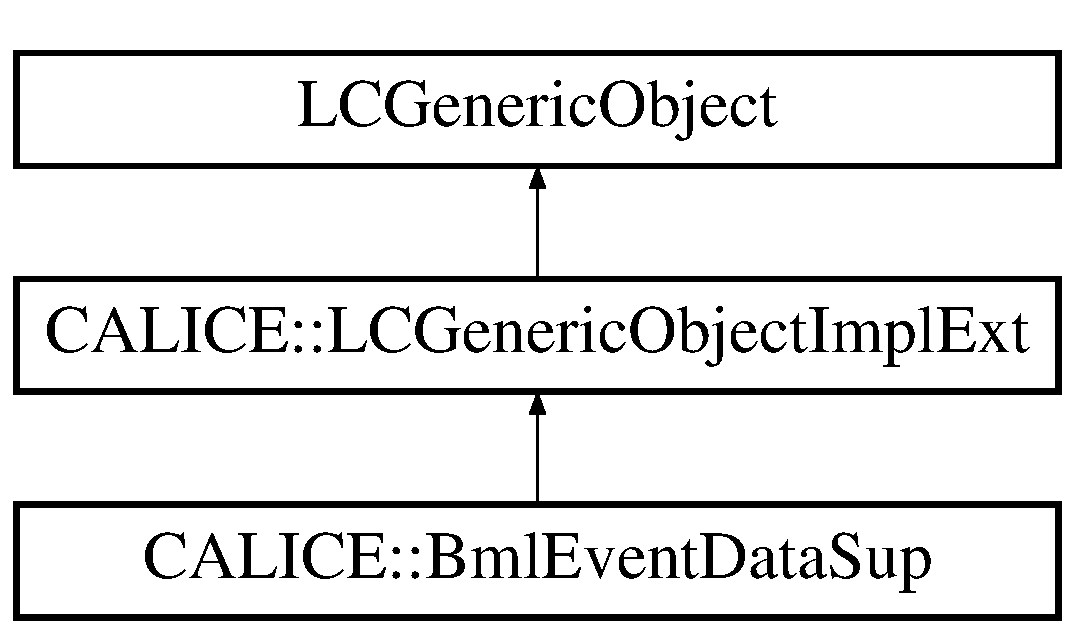
\includegraphics[height=3.000000cm]{classCALICE_1_1BmlEventDataSup}
\end{center}
\end{figure}
\subsection*{Private Member Functions}
\begin{DoxyCompactItemize}
\item 
{\bf Bml\-Event\-Data\-Sup} ()\label{classCALICE_1_1BmlEventDataSup_a1b777ba65db201936af16ba56dc197de}

\begin{DoxyCompactList}\small\item\em Default Constructor. \end{DoxyCompactList}\item 
{\bf Bml\-Event\-Data\-Sup} (L\-C\-Object $\ast${\bf obj})\label{classCALICE_1_1BmlEventDataSup_ababa5fa292e17ad8181dd30149f4d87e}

\begin{DoxyCompactList}\small\item\em A copy constructor. \end{DoxyCompactList}\item 
virtual {\bf $\sim$\-Bml\-Event\-Data\-Sup} ()\label{classCALICE_1_1BmlEventDataSup_a8b5715bd0afdd93a7a5573bede6c047a}

\begin{DoxyCompactList}\small\item\em The destructor. \end{DoxyCompactList}\item 
{\bf Bml\-Event\-Data\-Sup} \& {\bf set\-T\-D\-C\-Type} (std\-::string type\-Str)
\begin{DoxyCompactList}\small\item\em set the tdc type \end{DoxyCompactList}\item 
void {\bfseries set\-Pointer\-To\-Index\-Of\-Int\-Type\-Names} (int nameind)\label{classCALICE_1_1BmlEventDataSup_a9fa4191baf23435b722322fb1ca8b56e}

\item 
void {\bfseries set\-Length\-Index\-Of\-Int\-Type\-Names} (int lengthindex)\label{classCALICE_1_1BmlEventDataSup_ad5cfea715dbde1072b8c8a47f61c656e}

\item 
int {\bf get\-Length\-Index\-Of\-Int\-Type\-Names} () const \label{classCALICE_1_1BmlEventDataSup_a21ebe68dd1e819533a2af15879b1653d}

\begin{DoxyCompactList}\small\item\em Retrieve the index at which the lengths of the names of the int data types do start. \end{DoxyCompactList}\item 
int {\bf get\-Pointer\-To\-Index\-Of\-Int\-Type\-Names} () const \label{classCALICE_1_1BmlEventDataSup_afc31491a2fe74e80c3bf4b98b1a6ec1c}

\begin{DoxyCompactList}\small\item\em Retrieve the index at which the pointer to the names of int data types do start. \end{DoxyCompactList}\item 
void {\bf set\-Type\-Index} (int pos, int value)\label{classCALICE_1_1BmlEventDataSup_afeadf8495ac708b6eb4f372e262b4115}

\begin{DoxyCompactList}\small\item\em Set the index of a given data type name. \end{DoxyCompactList}\item 
std\-::string {\bf get\-T\-D\-C\-Type} () const 
\begin{DoxyCompactList}\small\item\em get the tdc type \end{DoxyCompactList}\item 
{\bf Bml\-Event\-Data\-Sup} \& {\bf set\-Event\-Fifo\-Cont} (int fifocont)\label{classCALICE_1_1BmlEventDataSup_ac3263e6f4c8a3be3b1ca36308b0f32c8}

\begin{DoxyCompactList}\small\item\em Store the F\-I\-F\-O content. \end{DoxyCompactList}\item 
unsigned short {\bf get\-Event\-Count} () const \label{classCALICE_1_1BmlEventDataSup_a1284d5d9b342180a65d3aef2cd593a50}

\begin{DoxyCompactList}\small\item\em get the event count \end{DoxyCompactList}\item 
unsigned short {\bf get\-Word\-Count} () const \label{classCALICE_1_1BmlEventDataSup_a75f899e45c6c056103e25fce6acb0851}

\begin{DoxyCompactList}\small\item\em get the word count \end{DoxyCompactList}\item 
{\bf Bml\-Event\-Data\-Sup} \& {\bf set\-Bunch\-I\-D} (int bunchid)\label{classCALICE_1_1BmlEventDataSup_acef67a0bc90854904fb4382501ecaf8d}

\begin{DoxyCompactList}\small\item\em set the bunch id \end{DoxyCompactList}\item 
int {\bf get\-Bunch\-I\-D} () const \label{classCALICE_1_1BmlEventDataSup_a402a35429e1fb4cefc030246d6a7dc8d}

\begin{DoxyCompactList}\small\item\em get the bunch id \end{DoxyCompactList}\item 
{\bf Bml\-Event\-Data\-Sup} \& {\bf set\-Event\-I\-D\-Trailer} (int event\-I\-D\-Trailer)\label{classCALICE_1_1BmlEventDataSup_ac1a762c3a809585cb908e1f9edce15ac}

\begin{DoxyCompactList}\small\item\em Set the eventid from the T\-D\-C trailer. \end{DoxyCompactList}\item 
short {\bf get\-Event\-I\-D\-Trailer} () const \label{classCALICE_1_1BmlEventDataSup_af98ba50b8fb39a943bc35067ffaf337b}

\begin{DoxyCompactList}\small\item\em Return the eventid from the T\-D\-C trailer. \end{DoxyCompactList}\item 
{\bf Bml\-Event\-Data\-Sup} \& {\bf set\-T\-D\-C\-Errors} (int tdc\-Errors)\label{classCALICE_1_1BmlEventDataSup_a812f9190cf1962203e1588669fc98f25}

\begin{DoxyCompactList}\small\item\em Set the T\-D\-C errors. \end{DoxyCompactList}\item 
int {\bf get\-T\-D\-C\-Errors} () const \label{classCALICE_1_1BmlEventDataSup_a53367b022e3100a0e3bd613ef2b70935}

\begin{DoxyCompactList}\small\item\em Get the T\-D\-C errors. \end{DoxyCompactList}\item 
{\bf Bml\-Event\-Data\-Sup} \& {\bf set\-Buffer\-Overflow} (int buffer\-Overflow)\label{classCALICE_1_1BmlEventDataSup_a90c7ac60defd7bb8a827f1aea40aedc6}

\begin{DoxyCompactList}\small\item\em Set the buffer overflow. \end{DoxyCompactList}\item 
int {\bf get\-Buffer\-Overflow} () const \label{classCALICE_1_1BmlEventDataSup_a5d6652dad161f253768ae01418d2c669}

\begin{DoxyCompactList}\small\item\em Get the buffer overflow. \end{DoxyCompactList}\item 
{\bf Bml\-Event\-Data\-Sup} \& {\bf set\-Trigger\-Lost} (int triggerlost)\label{classCALICE_1_1BmlEventDataSup_ad432619ccacb13abb181a12ab4662822}

\begin{DoxyCompactList}\small\item\em Set the number of words in the trailer. \end{DoxyCompactList}\item 
int {\bf get\-Trigger\-Lost} () const \label{classCALICE_1_1BmlEventDataSup_a7110357892a453499f8e3bbd2b0ff535}

\begin{DoxyCompactList}\small\item\em Get the number of lost triggers. \end{DoxyCompactList}\item 
{\bf Bml\-Event\-Data\-Sup} \& {\bf set\-T\-D\-C\-Word\-Count\-Trailer} (int numwords)\label{classCALICE_1_1BmlEventDataSup_aa8e12d29d2060db9c3657a6e4f9d8ac7}

\begin{DoxyCompactList}\small\item\em Set the number of lost triggers. \end{DoxyCompactList}\item 
int {\bf get\-T\-D\-C\-Word\-Count\-Trailer} () const \label{classCALICE_1_1BmlEventDataSup_a688bc2f933ce1011e4a03ca904539f3c}

\begin{DoxyCompactList}\small\item\em Get the number of words in the trailer. \end{DoxyCompactList}\item 
const std\-::string {\bf get\-Type\-Name} () const \label{classCALICE_1_1BmlEventDataSup_a075786d44470d270e1e931bcfa896394}

\begin{DoxyCompactList}\small\item\em returns the the type name \end{DoxyCompactList}\item 
const std\-::string {\bf get\-Data\-Description} () const \label{classCALICE_1_1BmlEventDataSup_acebe6fba59eced039cc6bad225e9bc71}

\begin{DoxyCompactList}\small\item\em returns a brief description of the data stored \end{DoxyCompactList}\item 
std\-::ostream \& {\bf print} (std\-::ostream \&ostrmsup)\label{classCALICE_1_1BmlEventDataSup_ae4684c1d74d640dd5b4258d1af5d2e70}

\begin{DoxyCompactList}\small\item\em dumps data content \end{DoxyCompactList}\end{DoxyCompactItemize}
\subsection*{Friends}
\begin{DoxyCompactItemize}
\item 
class {\bfseries Bml\-Event\-Data}\label{classCALICE_1_1BmlEventDataSup_af03b3108e540123cf6fb29facde51e29}

\end{DoxyCompactItemize}
\subsection*{Additional Inherited Members}


\subsection{Detailed Description}
Class to store supplementary \doxyref{Bml\-Event\-Data}{p.}{classCALICE_1_1BmlEventData}. 

This is tailored to the data extracted from the Caen T\-D\-Cs in extension of the actual class \doxyref{Bml\-Event\-Data}{p.}{classCALICE_1_1BmlEventData} This class is written such that it should be only accessed via the aforementioned class The user is strongly discouraged to instantiate by him/herself. It has only private functions and declares \doxyref{Bml\-Event\-Data}{p.}{classCALICE_1_1BmlEventData} to be its friend. \begin{DoxyAuthor}{Author}
R. P�schl (L\-A\-L Orsay) 
\end{DoxyAuthor}
\begin{DoxyDate}{Date}
Oct 13 2010 
\end{DoxyDate}


Definition at line 52 of file Bml\-Event\-Data\-Sup.\-hh.



\subsection{Member Function Documentation}
\index{C\-A\-L\-I\-C\-E\-::\-Bml\-Event\-Data\-Sup@{C\-A\-L\-I\-C\-E\-::\-Bml\-Event\-Data\-Sup}!get\-T\-D\-C\-Type@{get\-T\-D\-C\-Type}}
\index{get\-T\-D\-C\-Type@{get\-T\-D\-C\-Type}!CALICE::BmlEventDataSup@{C\-A\-L\-I\-C\-E\-::\-Bml\-Event\-Data\-Sup}}
\subsubsection[{get\-T\-D\-C\-Type}]{\setlength{\rightskip}{0pt plus 5cm}std\-::string C\-A\-L\-I\-C\-E\-::\-Bml\-Event\-Data\-Sup\-::get\-T\-D\-C\-Type (
\begin{DoxyParamCaption}
{}
\end{DoxyParamCaption}
) const\hspace{0.3cm}{\ttfamily [inline]}, {\ttfamily [private]}}\label{classCALICE_1_1BmlEventDataSup_a2e28417799fb6b46b4fd5bd798bffed3}


get the tdc type 

Currently since only one string in object -\/$>$ to be modified if more strings 

Definition at line 144 of file Bml\-Event\-Data\-Sup.\-hh.



References C\-A\-L\-I\-C\-E\-::get\-String\-From\-Ints().



Referenced by print().

\index{C\-A\-L\-I\-C\-E\-::\-Bml\-Event\-Data\-Sup@{C\-A\-L\-I\-C\-E\-::\-Bml\-Event\-Data\-Sup}!set\-T\-D\-C\-Type@{set\-T\-D\-C\-Type}}
\index{set\-T\-D\-C\-Type@{set\-T\-D\-C\-Type}!CALICE::BmlEventDataSup@{C\-A\-L\-I\-C\-E\-::\-Bml\-Event\-Data\-Sup}}
\subsubsection[{set\-T\-D\-C\-Type}]{\setlength{\rightskip}{0pt plus 5cm}{\bf Bml\-Event\-Data\-Sup}\& C\-A\-L\-I\-C\-E\-::\-Bml\-Event\-Data\-Sup\-::set\-T\-D\-C\-Type (
\begin{DoxyParamCaption}
\item[{std\-::string}]{type\-Str}
\end{DoxyParamCaption}
)\hspace{0.3cm}{\ttfamily [inline]}, {\ttfamily [private]}}\label{classCALICE_1_1BmlEventDataSup_ab3677309acfd81396e1333ff9b967f2a}


set the tdc type 

Store the index at which the pointer to the names of the int data data types do start

This written such that it can be extended in case more strings need to be stored

Would however trigger a bit of re-\/writing but at least it {\itshape sure} that it remains always

compatible and flexible

We use the same ugly but successful technique as in \doxyref{Daq\-Type\-Data\-Block}{p.}{classCALICE_1_1DaqTypeDataBlock} (we may even be able to inherit from it

now we've simply copied a few useful methods -\/$>$ to be checked 

Definition at line 94 of file Bml\-Event\-Data\-Sup.\-hh.



References C\-A\-L\-I\-C\-E\-::convert\-String\-To\-Ints().



The documentation for this class was generated from the following files\-:\begin{DoxyCompactItemize}
\item 
Bml\-Event\-Data\-Sup.\-hh\item 
Bml\-Event\-Data\-Sup.\-cc\end{DoxyCompactItemize}

\section{C\-A\-L\-I\-C\-E\-:\-:Bml\-Slow\-Run\-Data\-Block Class Reference}
\label{classCALICE_1_1BmlSlowRunDataBlock}\index{C\-A\-L\-I\-C\-E\-::\-Bml\-Slow\-Run\-Data\-Block@{C\-A\-L\-I\-C\-E\-::\-Bml\-Slow\-Run\-Data\-Block}}


Interface Class to access the Bml\-Slow\-Run Data Here we handle ahc voltages, temperatures et al.  




{\ttfamily \#include $<$Bml\-Slow\-Run\-Data\-Block.\-hh$>$}

Inheritance diagram for C\-A\-L\-I\-C\-E\-:\-:Bml\-Slow\-Run\-Data\-Block\-:\begin{figure}[H]
\begin{center}
\leavevmode
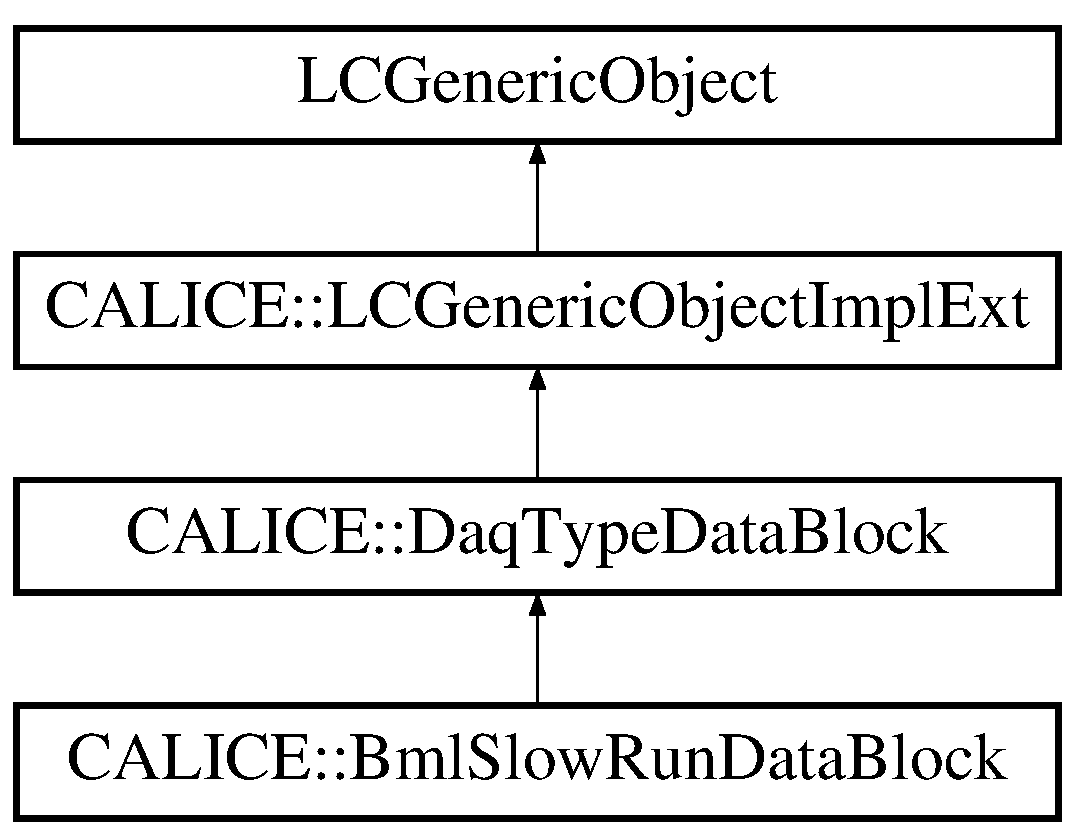
\includegraphics[height=4.000000cm]{classCALICE_1_1BmlSlowRunDataBlock}
\end{center}
\end{figure}
\subsection*{Public Member Functions}
\begin{DoxyCompactItemize}
\item 
{\bf Bml\-Slow\-Run\-Data\-Block} ()\label{classCALICE_1_1BmlSlowRunDataBlock_a25c7a935d4873ff7065def913bf1c77c}

\begin{DoxyCompactList}\small\item\em Constructor. \end{DoxyCompactList}\item 
{\bf Bml\-Slow\-Run\-Data\-Block} (L\-C\-Object $\ast${\bf obj})\label{classCALICE_1_1BmlSlowRunDataBlock_ae4960ae7344e47dd4061e4a97067cce9}

\begin{DoxyCompactList}\small\item\em 'Copy constructor' needed to interpret L\-C\-Collection read from file/database. \end{DoxyCompactList}\item 
{\bf Bml\-Slow\-Run\-Data\-Block} \& {\bf set\-Absorber\-Position} (double abspos)
\begin{DoxyCompactList}\small\item\em Store the aborber position device in cern h6b beamline to purify beam, ie. \end{DoxyCompactList}\item 
double {\bf get\-Absorber\-Position} () const \label{classCALICE_1_1BmlSlowRunDataBlock_a2eeaa6e8341b068b991d1c7ec42a0e8c}

\begin{DoxyCompactList}\small\item\em Retrieve the absorber position. \end{DoxyCompactList}\item 
{\bf Bml\-Slow\-Run\-Data\-Block} \& {\bf set\-Time\-Stamp} (struct tm $\ast$timestamp)\label{classCALICE_1_1BmlSlowRunDataBlock_aaeaa4c4d05400ff8e10dca94acde6b5d}

\begin{DoxyCompactList}\small\item\em Sets the time stamp We store Year, Month, Day and Hour, Minute, Second We store U\-T\-C!!!! \end{DoxyCompactList}\item 
L\-C\-Time {\bf get\-Time\-Stamp} () const \label{classCALICE_1_1BmlSlowRunDataBlock_ae4bf5b8cb65578245c68add8a874e5a4}

\begin{DoxyCompactList}\small\item\em returns the start stamp \end{DoxyCompactList}\item 
L\-C\-Time {\bf get\-Time\-Stamp\-Bml} ()\label{classCALICE_1_1BmlSlowRunDataBlock_aa8e2d5f73a3ee0de0c6a0ebd972b4f23}

\begin{DoxyCompactList}\small\item\em Implementation of the method to obtain the timestamp as given by the beamline operators here identical to the only timestamp which was stored. \end{DoxyCompactList}\item 
L\-C\-Time {\bf get\-Time\-Stamp\-Daq} ()\label{classCALICE_1_1BmlSlowRunDataBlock_a04c8788e599ae8873d81b515d67c9f93}

\begin{DoxyCompactList}\small\item\em Implementation of the method to obtain the timestamp as given by the calice daq Here 0 as no timestamp has been stored. \end{DoxyCompactList}\item 
{\bf Bml\-Slow\-Run\-Data\-Block} \& {\bf set\-T4\-Position} (double t4pos)\label{classCALICE_1_1BmlSlowRunDataBlock_ac16185be4c02fc71f31e8773bebc9e19}

\begin{DoxyCompactList}\small\item\em Store the t4 position device in cern h6b beamline to produce desired particles out of the secondary beam. \end{DoxyCompactList}\item 
double {\bf get\-T4\-Position} () const \label{classCALICE_1_1BmlSlowRunDataBlock_a608e9bbb5084e0960e608fd9b3ece877}

\begin{DoxyCompactList}\small\item\em Retrieve the absorber position. \end{DoxyCompactList}\item 
{\bf Bml\-Slow\-Run\-Data\-Block} \& {\bf set\-Target\-Position} (double targetpos)\label{classCALICE_1_1BmlSlowRunDataBlock_af3938577d279f22be257af9838c3e34e}

\begin{DoxyCompactList}\small\item\em Store the target position primary target hit by ythe S\-P\-S beam. \end{DoxyCompactList}\item 
double {\bf get\-Target\-Position} () const \label{classCALICE_1_1BmlSlowRunDataBlock_a8da787f3406d21c331f11fb449fe33a2}

\begin{DoxyCompactList}\small\item\em Retrieve the target position. \end{DoxyCompactList}\item 
const std\-::vector$<$ double $>$ \& {\bf get\-Sextapole\-Currents} () const 
\begin{DoxyCompactList}\small\item\em Retrieve the sextapole currents The values are stored in the sequence 'Measurement, Reference e.\-g. \end{DoxyCompactList}\item 
const std\-::vector$<$ double $>$ \& {\bf get\-Bend\-Currents} () const 
\begin{DoxyCompactList}\small\item\em Retrieve the bending magnet currents. \end{DoxyCompactList}\item 
const std\-::vector$<$ double $>$ \& {\bf get\-Collimator\-Positions} () const 
\begin{DoxyCompactList}\small\item\em Retrieve the collimator positions The values are stored in the sequence 'Measurement x, Reference x, Meaurement y, Reference y e.\-g. \end{DoxyCompactList}\item 
const std\-::vector$<$ double $>$ \& {\bf get\-Quadrupole\-Currents} () const 
\begin{DoxyCompactList}\small\item\em Retrieve the quadrupole currents. \end{DoxyCompactList}\item 
const std\-::vector$<$ double $>$ \& {\bf get\-Trim\-Currents} () const 
\begin{DoxyCompactList}\small\item\em Retrieve the trim currents. \end{DoxyCompactList}\item 
const std\-::vector$<$ int $>$ \& {\bf get\-H6a\-Experiment\-Counts} () const \label{classCALICE_1_1BmlSlowRunDataBlock_a2b07ebc901bf88e683528599b036b725}

\begin{DoxyCompactList}\small\item\em Retrieve the h6a experiment count. \end{DoxyCompactList}\item 
const std\-::vector$<$ int $>$ \& {\bf get\-H6b\-Experiment\-Counts} () const \label{classCALICE_1_1BmlSlowRunDataBlock_a045906ccd4541632f32c0225b48a0ed6}

\begin{DoxyCompactList}\small\item\em Retrieve the h6b experiment count. \end{DoxyCompactList}\item 
const std\-::vector$<$ int $>$ \& {\bf get\-H6c\-Experiment\-Counts} () const \label{classCALICE_1_1BmlSlowRunDataBlock_a28ff6638d17e96f8f30563baef733163}

\begin{DoxyCompactList}\small\item\em Retrieve the h6c experiment count. \end{DoxyCompactList}\item 
const std\-::vector$<$ int $>$ \& {\bf get\-Rp\-Experiment\-Counts} () const \label{classCALICE_1_1BmlSlowRunDataBlock_af567cfeefd9feb1ecab1a2c2b139e1f0}

\begin{DoxyCompactList}\small\item\em Retrieve the rp experiment count. \end{DoxyCompactList}\item 
const std\-::vector$<$ int $>$ \& {\bf get\-Scintillator\-Counts} () const \label{classCALICE_1_1BmlSlowRunDataBlock_a03765d06e1ca48d6d9529b6ea856e3ae}

\begin{DoxyCompactList}\small\item\em Retrieve the scintillator count. \end{DoxyCompactList}\item 
void {\bf set\-Dbl\-Arrays} (const {\bf Daq\-Type\-Data\-Dbl\-Map\-\_\-t} \&)\label{classCALICE_1_1BmlSlowRunDataBlock_ad45a9c9a2b9ed10dc062dd68b60838d1}

\begin{DoxyCompactList}\small\item\em These methods receive the vectors with the measured values Mainly to store large arrays of a given datatype but in principle this can be extended to every entry in the interface class. \end{DoxyCompactList}\item 
void {\bfseries set\-Float\-Arrays} (const Daq\-Type\-Data\-Float\-Map\-\_\-t \&)\label{classCALICE_1_1BmlSlowRunDataBlock_afeec6359c43f0e651899ca13d713846c}

\item 
void {\bfseries set\-Int\-Arrays} (const Daq\-Type\-Data\-U\-Int\-Map\-\_\-t \&)\label{classCALICE_1_1BmlSlowRunDataBlock_a188d4b95271b83a3a439aa6ffc15efd8}

\item 
const double {\bf get\-Beam\-Energy} ()\label{classCALICE_1_1BmlSlowRunDataBlock_a2894d5f9fe5b2cb47c59984a8d98340f}

\begin{DoxyCompactList}\small\item\em Implementation of the method to get the beam energy. \end{DoxyCompactList}\item 
void {\bf print} (std\-::ostream \&)
\begin{DoxyCompactList}\small\item\em convenient print method \end{DoxyCompactList}\item 
const std\-::string {\bf get\-Type\-Name} () const \label{classCALICE_1_1BmlSlowRunDataBlock_a634733a4540fed14c4a967db1eb065e2}

\begin{DoxyCompactList}\small\item\em Return the type of the class. \end{DoxyCompactList}\item 
const std\-::string {\bf get\-Data\-Description} () const \label{classCALICE_1_1BmlSlowRunDataBlock_a6e1e0b78c1419825b0aed68058596001}

\begin{DoxyCompactList}\small\item\em Return a brief description of the data members. \end{DoxyCompactList}\end{DoxyCompactItemize}
\subsection*{Private Types}
\begin{DoxyCompactItemize}
\item 
typedef std\-::map$<$ string, \\*
std\-::pair$<$ int, std\-::vector\\*
$<$ double $>$ $\ast$ $>$ $>$ {\bf Bml\-Sro\-Types\-Dbl\-Map\-\_\-t}\label{classCALICE_1_1BmlSlowRunDataBlock_a5b364de391c94a82921db206b900186e}

\begin{DoxyCompactList}\small\item\em Relation between the datatype its position among the tuple of double vals and the vector the data are readinto. \end{DoxyCompactList}\item 
typedef std\-::map$<$ string, \\*
std\-::pair$<$ int, std\-::vector\\*
$<$ int $>$ $\ast$ $>$ $>$ {\bfseries Bml\-Sro\-Types\-Int\-Map\-\_\-t}\label{classCALICE_1_1BmlSlowRunDataBlock_a813a5320e33a8d2d56356fbeefd2773c}

\item 
typedef std\-::map$<$ string, \\*
std\-::pair$<$ int, std\-::vector\\*
$<$ float $>$ $\ast$ $>$ $>$ {\bfseries Bml\-Sro\-Types\-Float\-Map\-\_\-t}\label{classCALICE_1_1BmlSlowRunDataBlock_ae6c9fd754e494387de40e650475b5bf4}

\end{DoxyCompactItemize}
\subsection*{Private Member Functions}
\begin{DoxyCompactItemize}
\item 
void {\bf set\-Num\-Pos} (int posindex, int pos, int numvals)\label{classCALICE_1_1BmlSlowRunDataBlock_a6870f445e1d13706fcfc2debe4ef1cc8}

\begin{DoxyCompactList}\small\item\em Store the position and number of measured values for a given datatype. \end{DoxyCompactList}\item 
int {\bf get\-Pos} (int posindex) const \label{classCALICE_1_1BmlSlowRunDataBlock_a06931182e3ea56d8e529251cd432dd68}

\begin{DoxyCompactList}\small\item\em get the position of the given datatype within the array of values \end{DoxyCompactList}\item 
int {\bf get\-Num} (int posindex) const \label{classCALICE_1_1BmlSlowRunDataBlock_a223ca19f8e3d33c6914aa70d8372a456}

\begin{DoxyCompactList}\small\item\em Retrieve the number of measured values for a given datatype. \end{DoxyCompactList}\item 
void {\bf set\-Types} ()\label{classCALICE_1_1BmlSlowRunDataBlock_a1dc8f0b8e9b03d789d339e7788350cf4}

\begin{DoxyCompactList}\small\item\em This method defines the (general) types of the measured values A type not present here will not be treated!!! \end{DoxyCompactList}\item 
void {\bf prepare\-Output\-Vecs} ()\label{classCALICE_1_1BmlSlowRunDataBlock_ac84a8ae4e7d3c4a0d7fd3a00f5870b9e}

\begin{DoxyCompactList}\small\item\em A method which prepares the output vectors. \end{DoxyCompactList}\end{DoxyCompactItemize}
\subsection*{Private Attributes}
\begin{DoxyCompactItemize}
\item 
{\bf Bml\-Sro\-Types\-Dbl\-Map\-\_\-t} {\bf \-\_\-the\-Dbl\-Types}\label{classCALICE_1_1BmlSlowRunDataBlock_aea4514391e28cac4c31080c73a4b2bea}

\begin{DoxyCompactList}\small\item\em The vector which contains the types and to the position and values of the types doubles. \end{DoxyCompactList}\item 
Bml\-Sro\-Types\-Int\-Map\-\_\-t {\bfseries \-\_\-the\-Int\-Types}\label{classCALICE_1_1BmlSlowRunDataBlock_a7d0b680fa737df9349fcccd0db4b4e8f}

\item 
Bml\-Sro\-Types\-Float\-Map\-\_\-t {\bfseries \-\_\-the\-Float\-Types}\label{classCALICE_1_1BmlSlowRunDataBlock_a71e936bfa00fbd092a8612d38232b645}

\item 
std\-::vector$<$ double $>$ {\bf \-\_\-sextapole\-Currents}\label{classCALICE_1_1BmlSlowRunDataBlock_a6c50465fa94d760a83e74340c9f1fcc5}

\begin{DoxyCompactList}\small\item\em The output vectors. \end{DoxyCompactList}\item 
std\-::vector$<$ double $>$ {\bf \-\_\-bend\-Currents}\label{classCALICE_1_1BmlSlowRunDataBlock_af5573bc33aef8a7f88778066531dbb89}

\begin{DoxyCompactList}\small\item\em Bending Magnets currents. \end{DoxyCompactList}\item 
std\-::vector$<$ double $>$ {\bf \-\_\-col\-Positions}\label{classCALICE_1_1BmlSlowRunDataBlock_afc0cde9f2ff3c9eec2a21fd33af16e3d}

\begin{DoxyCompactList}\small\item\em Collimator Positions. \end{DoxyCompactList}\item 
std\-::vector$<$ double $>$ {\bf \-\_\-quadrupole\-Currents}\label{classCALICE_1_1BmlSlowRunDataBlock_a7cd4f230b7fc52d6d23ba10d16ae4936}

\begin{DoxyCompactList}\small\item\em Quadrupole Magnets Current. \end{DoxyCompactList}\item 
std\-::vector$<$ double $>$ {\bf \-\_\-trim\-Currents}\label{classCALICE_1_1BmlSlowRunDataBlock_ae60f6f97b266b9fc573404fbd6821541}

\begin{DoxyCompactList}\small\item\em Trim Magnets Current. \end{DoxyCompactList}\item 
std\-::vector$<$ int $>$ {\bfseries \-\_\-h6a\-Exp\-Counts}\label{classCALICE_1_1BmlSlowRunDataBlock_a32ae594ff07ea83ab20f57aefd862820}

\item 
std\-::vector$<$ int $>$ {\bfseries \-\_\-h6b\-Exp\-Counts}\label{classCALICE_1_1BmlSlowRunDataBlock_ab585417272e850290aa9cb5635cac09a}

\item 
std\-::vector$<$ int $>$ {\bfseries \-\_\-h6c\-Exp\-Counts}\label{classCALICE_1_1BmlSlowRunDataBlock_a45c08f992d5e1f52259c65c02d877535}

\item 
std\-::vector$<$ int $>$ {\bfseries \-\_\-rp\-Exp\-Counts}\label{classCALICE_1_1BmlSlowRunDataBlock_a6a57670546525f6f2b72ae16a092134e}

\item 
std\-::vector$<$ int $>$ {\bfseries \-\_\-scint\-Counts}\label{classCALICE_1_1BmlSlowRunDataBlock_aff82cd4c1be4a45b6e35986c1ebe3466}

\end{DoxyCompactItemize}
\subsection*{Additional Inherited Members}


\subsection{Detailed Description}
Interface Class to access the Bml\-Slow\-Run Data Here we handle ahc voltages, temperatures et al. 

when filling the class the string identifying the measured values has to be given first, a warning is issued if no indentifier is given for a given datatype. On the other hand this concerns just the filler of the class, i.\-e. the conversion where it is done once for all. See the print method at the end of the class for the meaning of the fields (as of 31/7/06) Use the interface methods to retrieve the data fields Note that the implemented functionality is essentially kept for backward compatibility only i.\-e. that if ever the cern 06/07 data will be converted again the data will be written in the same way into the db as before. In principle the functionality like writing to the db is to be made by the base class. Beamline parameters for datataking period $>$ 2007 should be written into the db using the methods of the base class. \begin{DoxyAuthor}{Author}
\-: Roman P�schl L\-A\-L/\-Orsay 
\end{DoxyAuthor}
\begin{DoxyDate}{Date}
Aug 2006, modified Sept. 2008 
\end{DoxyDate}


Definition at line 71 of file Bml\-Slow\-Run\-Data\-Block.\-hh.



\subsection{Member Function Documentation}
\index{C\-A\-L\-I\-C\-E\-::\-Bml\-Slow\-Run\-Data\-Block@{C\-A\-L\-I\-C\-E\-::\-Bml\-Slow\-Run\-Data\-Block}!get\-Bend\-Currents@{get\-Bend\-Currents}}
\index{get\-Bend\-Currents@{get\-Bend\-Currents}!CALICE::BmlSlowRunDataBlock@{C\-A\-L\-I\-C\-E\-::\-Bml\-Slow\-Run\-Data\-Block}}
\subsubsection[{get\-Bend\-Currents}]{\setlength{\rightskip}{0pt plus 5cm}const std\-::vector$<$double$>$\& C\-A\-L\-I\-C\-E\-::\-Bml\-Slow\-Run\-Data\-Block\-::get\-Bend\-Currents (
\begin{DoxyParamCaption}
{}
\end{DoxyParamCaption}
) const\hspace{0.3cm}{\ttfamily [inline]}}\label{classCALICE_1_1BmlSlowRunDataBlock_a5e5c3b31bdca8c61adbec66c1e4eb06b}


Retrieve the bending magnet currents. 

\begin{DoxySeeAlso}{See Also}
\doxyref{get\-Sextapole\-Currents()}{p.}{classCALICE_1_1BmlSlowRunDataBlock_a10397850ce61e30a9ebe7cb4c71958d5} 
\end{DoxySeeAlso}


Definition at line 248 of file Bml\-Slow\-Run\-Data\-Block.\-hh.



Referenced by C\-A\-L\-I\-C\-E\-::\-Beam\-Momentum\-::\-Beam\-Momentum(), and print().

\index{C\-A\-L\-I\-C\-E\-::\-Bml\-Slow\-Run\-Data\-Block@{C\-A\-L\-I\-C\-E\-::\-Bml\-Slow\-Run\-Data\-Block}!get\-Collimator\-Positions@{get\-Collimator\-Positions}}
\index{get\-Collimator\-Positions@{get\-Collimator\-Positions}!CALICE::BmlSlowRunDataBlock@{C\-A\-L\-I\-C\-E\-::\-Bml\-Slow\-Run\-Data\-Block}}
\subsubsection[{get\-Collimator\-Positions}]{\setlength{\rightskip}{0pt plus 5cm}const std\-::vector$<$double$>$\& C\-A\-L\-I\-C\-E\-::\-Bml\-Slow\-Run\-Data\-Block\-::get\-Collimator\-Positions (
\begin{DoxyParamCaption}
{}
\end{DoxyParamCaption}
) const\hspace{0.3cm}{\ttfamily [inline]}}\label{classCALICE_1_1BmlSlowRunDataBlock_a948e24e50bd1e30f45b115694ef70786}


Retrieve the collimator positions The values are stored in the sequence 'Measurement x, Reference x, Meaurement y, Reference y e.\-g. 

\-\_\-col\-Positions[0] = measured value of coll. 1 -\/ x coord. (counting from 1) e.\-g. \-\_\-col\-Positions[1] = reference value of coll. 1 -\/ x coord. (counting from 1) e.\-g. \-\_\-col\-Positions[2] = measured value of coll. 1 -\/ y coord. (counting from 1) e.\-g. \-\_\-col\-Positions[3] = reference value of coll. 1 -\/ y coord. (counting from 1) 

Definition at line 258 of file Bml\-Slow\-Run\-Data\-Block.\-hh.



Referenced by C\-A\-L\-I\-C\-E\-::\-Beam\-Momentum\-::\-Beam\-Momentum(), and print().

\index{C\-A\-L\-I\-C\-E\-::\-Bml\-Slow\-Run\-Data\-Block@{C\-A\-L\-I\-C\-E\-::\-Bml\-Slow\-Run\-Data\-Block}!get\-Quadrupole\-Currents@{get\-Quadrupole\-Currents}}
\index{get\-Quadrupole\-Currents@{get\-Quadrupole\-Currents}!CALICE::BmlSlowRunDataBlock@{C\-A\-L\-I\-C\-E\-::\-Bml\-Slow\-Run\-Data\-Block}}
\subsubsection[{get\-Quadrupole\-Currents}]{\setlength{\rightskip}{0pt plus 5cm}const std\-::vector$<$double$>$\& C\-A\-L\-I\-C\-E\-::\-Bml\-Slow\-Run\-Data\-Block\-::get\-Quadrupole\-Currents (
\begin{DoxyParamCaption}
{}
\end{DoxyParamCaption}
) const\hspace{0.3cm}{\ttfamily [inline]}}\label{classCALICE_1_1BmlSlowRunDataBlock_aaad60dbe13efa032b18a52a2eb246ec3}


Retrieve the quadrupole currents. 

\begin{DoxySeeAlso}{See Also}
\doxyref{get\-Sextapole\-Currents()}{p.}{classCALICE_1_1BmlSlowRunDataBlock_a10397850ce61e30a9ebe7cb4c71958d5} 
\end{DoxySeeAlso}


Definition at line 264 of file Bml\-Slow\-Run\-Data\-Block.\-hh.



Referenced by print().

\index{C\-A\-L\-I\-C\-E\-::\-Bml\-Slow\-Run\-Data\-Block@{C\-A\-L\-I\-C\-E\-::\-Bml\-Slow\-Run\-Data\-Block}!get\-Sextapole\-Currents@{get\-Sextapole\-Currents}}
\index{get\-Sextapole\-Currents@{get\-Sextapole\-Currents}!CALICE::BmlSlowRunDataBlock@{C\-A\-L\-I\-C\-E\-::\-Bml\-Slow\-Run\-Data\-Block}}
\subsubsection[{get\-Sextapole\-Currents}]{\setlength{\rightskip}{0pt plus 5cm}const std\-::vector$<$double$>$\& C\-A\-L\-I\-C\-E\-::\-Bml\-Slow\-Run\-Data\-Block\-::get\-Sextapole\-Currents (
\begin{DoxyParamCaption}
{}
\end{DoxyParamCaption}
) const\hspace{0.3cm}{\ttfamily [inline]}}\label{classCALICE_1_1BmlSlowRunDataBlock_a10397850ce61e30a9ebe7cb4c71958d5}


Retrieve the sextapole currents The values are stored in the sequence 'Measurement, Reference e.\-g. 

\-\_\-sextapole\-Currents[0] = measured value of sextupole 1 (counting from 1) e.\-g. \-\_\-sextapole\-Currents[1] = reference value of sextupole 1 (counting from 1) 

Definition at line 242 of file Bml\-Slow\-Run\-Data\-Block.\-hh.



Referenced by print().

\index{C\-A\-L\-I\-C\-E\-::\-Bml\-Slow\-Run\-Data\-Block@{C\-A\-L\-I\-C\-E\-::\-Bml\-Slow\-Run\-Data\-Block}!get\-Trim\-Currents@{get\-Trim\-Currents}}
\index{get\-Trim\-Currents@{get\-Trim\-Currents}!CALICE::BmlSlowRunDataBlock@{C\-A\-L\-I\-C\-E\-::\-Bml\-Slow\-Run\-Data\-Block}}
\subsubsection[{get\-Trim\-Currents}]{\setlength{\rightskip}{0pt plus 5cm}const std\-::vector$<$double$>$\& C\-A\-L\-I\-C\-E\-::\-Bml\-Slow\-Run\-Data\-Block\-::get\-Trim\-Currents (
\begin{DoxyParamCaption}
{}
\end{DoxyParamCaption}
) const\hspace{0.3cm}{\ttfamily [inline]}}\label{classCALICE_1_1BmlSlowRunDataBlock_a5a9b74416b5affcf70342f662cb52b5b}


Retrieve the trim currents. 

\begin{DoxySeeAlso}{See Also}
\doxyref{get\-Sextapole\-Currents()}{p.}{classCALICE_1_1BmlSlowRunDataBlock_a10397850ce61e30a9ebe7cb4c71958d5} 
\end{DoxySeeAlso}


Definition at line 270 of file Bml\-Slow\-Run\-Data\-Block.\-hh.



Referenced by print().

\index{C\-A\-L\-I\-C\-E\-::\-Bml\-Slow\-Run\-Data\-Block@{C\-A\-L\-I\-C\-E\-::\-Bml\-Slow\-Run\-Data\-Block}!print@{print}}
\index{print@{print}!CALICE::BmlSlowRunDataBlock@{C\-A\-L\-I\-C\-E\-::\-Bml\-Slow\-Run\-Data\-Block}}
\subsubsection[{print}]{\setlength{\rightskip}{0pt plus 5cm}void C\-A\-L\-I\-C\-E\-::\-Bml\-Slow\-Run\-Data\-Block\-::print (
\begin{DoxyParamCaption}
\item[{std\-::ostream \&}]{os}
\end{DoxyParamCaption}
)\hspace{0.3cm}{\ttfamily [virtual]}}\label{classCALICE_1_1BmlSlowRunDataBlock_ae6fbf1de7c0528d67d77fb55e9c32eea}


convenient print method 

Convenient print method. 

Reimplemented from {\bf C\-A\-L\-I\-C\-E\-::\-Daq\-Type\-Data\-Block} \doxyref{}{p.}{classCALICE_1_1DaqTypeDataBlock_a0ab5d656a67220cfc75fd842c29e1ac7}.



Definition at line 177 of file Bml\-Slow\-Run\-Data\-Block.\-cc.



References get\-Absorber\-Position(), get\-Bend\-Currents(), get\-Collimator\-Positions(), get\-H6a\-Experiment\-Counts(), get\-H6b\-Experiment\-Counts(), get\-H6c\-Experiment\-Counts(), get\-Quadrupole\-Currents(), get\-Rp\-Experiment\-Counts(), get\-Scintillator\-Counts(), get\-Sextapole\-Currents(), get\-T4\-Position(), get\-Target\-Position(), get\-Time\-Stamp(), get\-Trim\-Currents(), and prepare\-Output\-Vecs().

\index{C\-A\-L\-I\-C\-E\-::\-Bml\-Slow\-Run\-Data\-Block@{C\-A\-L\-I\-C\-E\-::\-Bml\-Slow\-Run\-Data\-Block}!set\-Absorber\-Position@{set\-Absorber\-Position}}
\index{set\-Absorber\-Position@{set\-Absorber\-Position}!CALICE::BmlSlowRunDataBlock@{C\-A\-L\-I\-C\-E\-::\-Bml\-Slow\-Run\-Data\-Block}}
\subsubsection[{set\-Absorber\-Position}]{\setlength{\rightskip}{0pt plus 5cm}{\bf Bml\-Slow\-Run\-Data\-Block}\& C\-A\-L\-I\-C\-E\-::\-Bml\-Slow\-Run\-Data\-Block\-::set\-Absorber\-Position (
\begin{DoxyParamCaption}
\item[{double}]{abspos}
\end{DoxyParamCaption}
)\hspace{0.3cm}{\ttfamily [inline]}}\label{classCALICE_1_1BmlSlowRunDataBlock_a6d982078b6aea53f9ec91cd2410dc3db}


Store the aborber position device in cern h6b beamline to purify beam, ie. 

to get rid of electrons 

Definition at line 134 of file Bml\-Slow\-Run\-Data\-Block.\-hh.



The documentation for this class was generated from the following files\-:\begin{DoxyCompactItemize}
\item 
Bml\-Slow\-Run\-Data\-Block.\-hh\item 
Bml\-Slow\-Run\-Data\-Block.\-cc\end{DoxyCompactItemize}

\section{C\-A\-L\-I\-C\-E\-:\-:Board\-I\-D Class Reference}
\label{classCALICE_1_1BoardID}\index{C\-A\-L\-I\-C\-E\-::\-Board\-I\-D@{C\-A\-L\-I\-C\-E\-::\-Board\-I\-D}}


Create a packed board id of crate, slot, component numbers and the label.  




{\ttfamily \#include $<$Board\-I\-D.\-hh$>$}

\subsection*{Public Member Functions}
\begin{DoxyCompactItemize}
\item 
{\bf Board\-I\-D} ()
\begin{DoxyCompactList}\small\item\em Create the packed id. \end{DoxyCompactList}\item 
{\bf Board\-I\-D} (const short crate\-I\-D, const short slot\-I\-D, const short board\-Component\-Number)\label{classCALICE_1_1BoardID_a7a77aa3cd232b76c491e51b97e70466e}

\begin{DoxyCompactList}\small\item\em Label does not belong to the Device I\-D since it ony indicates whether data were written or read back. \end{DoxyCompactList}\item 
{\bf Board\-I\-D} (const unsigned int packed\-\_\-id)
\begin{DoxyCompactList}\small\item\em Wrap interface around packed id. \end{DoxyCompactList}\item 
short {\bf get\-Crate\-I\-D} () const \label{classCALICE_1_1BoardID_a21bcc5f005a519c857eb9084081a5076}

\begin{DoxyCompactList}\small\item\em Unpack the crate id. \end{DoxyCompactList}\item 
short {\bf get\-Slot\-I\-D} () const \label{classCALICE_1_1BoardID_ad14869e733b4949a9266ae609cf31167}

\begin{DoxyCompactList}\small\item\em Unpack the slot id. \end{DoxyCompactList}\item 
short {\bf get\-Board\-Component\-Number} () const \label{classCALICE_1_1BoardID_aeff4d82392ef0af0fe036e1dd7edad0b}

\begin{DoxyCompactList}\small\item\em Unpack the board component number. \end{DoxyCompactList}\item 
unsigned int {\bf id} () const 
\begin{DoxyCompactList}\small\item\em Unpack the board label. \end{DoxyCompactList}\item 
{\bf operator unsigned int} ()\label{classCALICE_1_1BoardID_a6d639d0cd155108c97a48ca5c368917a}

\begin{DoxyCompactList}\small\item\em Get the packed id. \end{DoxyCompactList}\end{DoxyCompactItemize}
\subsection*{Private Attributes}
\begin{DoxyCompactItemize}
\item 
unsigned int {\bfseries \-\_\-id}\label{classCALICE_1_1BoardID_a77bc700e4cebf6b6a3dddb421ee5fd6b}

\end{DoxyCompactItemize}
\subsection*{Friends}
\begin{DoxyCompactItemize}
\item 
bool const {\bf operator$<$} (const {\bf Board\-I\-D} \&b1, const {\bf Board\-I\-D} \&b2)\label{classCALICE_1_1BoardID_a53050a9db904e5e5bdbb5a167c5a29dd}

\begin{DoxyCompactList}\small\item\em Compiler complained about missing $<$, $>$ operators when \doxyref{Board\-I\-D}{p.}{classCALICE_1_1BoardID} was directly used in a map, therefore we overload this operators. \end{DoxyCompactList}\item 
bool const {\bf operator$>$} (const {\bf Board\-I\-D} \&b1, const {\bf Board\-I\-D} \&b2)
\begin{DoxyCompactList}\small\item\em See above ... \end{DoxyCompactList}\end{DoxyCompactItemize}


\subsection{Detailed Description}
Create a packed board id of crate, slot, component numbers and the label. 

Class is cheap and can be used to generate a packed board id\-: unsigned int packed\-\_\-id = Board\-I\-D(short crate\-I\-D, short slot\-I\-D, short board\-Component\-Number, short board\-Label).\doxyref{id()}{p.}{classCALICE_1_1BoardID_a6079e4bcda24933f67f573b877c6746e}; or unsigned int packed\-\_\-id = Board\-I\-D(short crate\-I\-D, short slot\-I\-D, short board\-Component\-Number, short board\-Label); 

Definition at line 17 of file Board\-I\-D.\-hh.



\subsection{Constructor \& Destructor Documentation}
\index{C\-A\-L\-I\-C\-E\-::\-Board\-I\-D@{C\-A\-L\-I\-C\-E\-::\-Board\-I\-D}!Board\-I\-D@{Board\-I\-D}}
\index{Board\-I\-D@{Board\-I\-D}!CALICE::BoardID@{C\-A\-L\-I\-C\-E\-::\-Board\-I\-D}}
\subsubsection[{Board\-I\-D}]{\setlength{\rightskip}{0pt plus 5cm}C\-A\-L\-I\-C\-E\-::\-Board\-I\-D\-::\-Board\-I\-D (
\begin{DoxyParamCaption}
{}
\end{DoxyParamCaption}
)\hspace{0.3cm}{\ttfamily [inline]}}\label{classCALICE_1_1BoardID_a0bbfeabb419fbdf6823504cd844a9a91}


Create the packed id. 

default constructor. The default constructor produces an illegal board id. 

Definition at line 29 of file Board\-I\-D.\-hh.

\index{C\-A\-L\-I\-C\-E\-::\-Board\-I\-D@{C\-A\-L\-I\-C\-E\-::\-Board\-I\-D}!Board\-I\-D@{Board\-I\-D}}
\index{Board\-I\-D@{Board\-I\-D}!CALICE::BoardID@{C\-A\-L\-I\-C\-E\-::\-Board\-I\-D}}
\subsubsection[{Board\-I\-D}]{\setlength{\rightskip}{0pt plus 5cm}C\-A\-L\-I\-C\-E\-::\-Board\-I\-D\-::\-Board\-I\-D (
\begin{DoxyParamCaption}
\item[{const unsigned int}]{packed\-\_\-id}
\end{DoxyParamCaption}
)\hspace{0.3cm}{\ttfamily [inline]}}\label{classCALICE_1_1BoardID_a0c4690a0e17a9dc665e14525b70b3b24}


Wrap interface around packed id. 

Cheap method to decode the packed components. slot\-\_\-id=Board\-I\-D(packed\-\_\-id).\doxyref{get\-Slot\-I\-D()}{p.}{classCALICE_1_1BoardID_ad14869e733b4949a9266ae609cf31167}; 

Definition at line 49 of file Board\-I\-D.\-hh.



\subsection{Member Function Documentation}
\index{C\-A\-L\-I\-C\-E\-::\-Board\-I\-D@{C\-A\-L\-I\-C\-E\-::\-Board\-I\-D}!id@{id}}
\index{id@{id}!CALICE::BoardID@{C\-A\-L\-I\-C\-E\-::\-Board\-I\-D}}
\subsubsection[{id}]{\setlength{\rightskip}{0pt plus 5cm}unsigned int C\-A\-L\-I\-C\-E\-::\-Board\-I\-D\-::id (
\begin{DoxyParamCaption}
{}
\end{DoxyParamCaption}
) const\hspace{0.3cm}{\ttfamily [inline]}}\label{classCALICE_1_1BoardID_a6079e4bcda24933f67f573b877c6746e}


Unpack the board label. 

Get the packed id. 

Definition at line 80 of file Board\-I\-D.\-hh.



Referenced by C\-A\-L\-I\-C\-E\-::operator$>$().



\subsection{Friends And Related Function Documentation}
\index{C\-A\-L\-I\-C\-E\-::\-Board\-I\-D@{C\-A\-L\-I\-C\-E\-::\-Board\-I\-D}!operator$>$@{operator$>$}}
\index{operator$>$@{operator$>$}!CALICE::BoardID@{C\-A\-L\-I\-C\-E\-::\-Board\-I\-D}}
\subsubsection[{operator$>$}]{\setlength{\rightskip}{0pt plus 5cm}bool const operator$>$ (
\begin{DoxyParamCaption}
\item[{const {\bf Board\-I\-D} \&}]{b1, }
\item[{const {\bf Board\-I\-D} \&}]{b2}
\end{DoxyParamCaption}
)\hspace{0.3cm}{\ttfamily [friend]}}\label{classCALICE_1_1BoardID_a434e3e7f9f569d6d01ff7e57aebbf3de}


See above ... 



Definition at line 101 of file Board\-I\-D.\-hh.



The documentation for this class was generated from the following file\-:\begin{DoxyCompactItemize}
\item 
Board\-I\-D.\-hh\end{DoxyCompactItemize}

\section{C\-A\-L\-I\-C\-E\-:\-:Calibration\-Writer Class Reference}
\label{classCALICE_1_1CalibrationWriter}\index{C\-A\-L\-I\-C\-E\-::\-Calibration\-Writer@{C\-A\-L\-I\-C\-E\-::\-Calibration\-Writer}}


Class which handles the module wise storage of conditions data and the access to the lccd framework (i.\-e.  




{\ttfamily \#include $<$Calibration\-Writer.\-hh$>$}

\subsection*{Public Member Functions}
\begin{DoxyCompactItemize}
\item 
{\bf Calibration\-Writer} (std\-::string dbinit, std\-::string folder, std\-::string description)
\begin{DoxyCompactList}\small\item\em Constructor has parameters\-: \end{DoxyCompactList}\item 
void {\bf put\-Calibration} (unsigned module\-I\-D, unsigned cell\-Key, {\bf L\-C\-Hcal\-Calibration\-Object} $\ast$Calibration)
\begin{DoxyCompactList}\small\item\em fills the \char`\"{}memory\char`\"{} with a calibration object for a certain module\-I\-D and cell\-Key \end{DoxyCompactList}\item 
void {\bf put\-Calibration} (unsigned module\-I\-D, unsigned chip, unsigned channel, {\bf L\-C\-Hcal\-Calibration\-Object} $\ast$Calibration)
\begin{DoxyCompactList}\small\item\em fills the \char`\"{}memory\char`\"{} with a calibration object for a certain module\-I\-D and cell\-Key \end{DoxyCompactList}\item 
void {\bf flush\-Calibration} (lccd\-::\-L\-C\-C\-D\-Time\-Stamp from, lccd\-::\-L\-C\-C\-D\-Time\-Stamp till, bool \-\_\-write\-File) const 
\begin{DoxyCompactList}\small\item\em writes the \char`\"{}memory\char`\"{} to the given data base and the given folder, extraction time range is set equal to the validity time range \end{DoxyCompactList}\item 
void {\bf flush\-Calibration} (lccd\-::\-L\-C\-C\-D\-Time\-Stamp from, lccd\-::\-L\-C\-C\-D\-Time\-Stamp till, lccd\-::\-L\-C\-C\-D\-Time\-Stamp extraction\-Time, bool \-\_\-write\-File) const 
\begin{DoxyCompactList}\small\item\em writes the \char`\"{}memory\char`\"{} to the given data base and the given folder \end{DoxyCompactList}\item 
void {\bf flush\-Calibration} (lccd\-::\-L\-C\-C\-D\-Time\-Stamp from, lccd\-::\-L\-C\-C\-D\-Time\-Stamp till, lccd\-::\-L\-C\-C\-D\-Time\-Stamp extraction\-From, lccd\-::\-L\-C\-C\-D\-Time\-Stamp extraction\-Till, bool \-\_\-write\-File) const 
\begin{DoxyCompactList}\small\item\em writes the \char`\"{}memory\char`\"{} to the given data base and the given folder \end{DoxyCompactList}\end{DoxyCompactItemize}
\subsection*{Protected Attributes}
\begin{DoxyCompactItemize}
\item 
std\-::string {\bf \-\_\-dbinit}\label{classCALICE_1_1CalibrationWriter_adbf1bd238e3c2be0a0d37415374ef407}

\begin{DoxyCompactList}\small\item\em access string for the mysql database \end{DoxyCompactList}\item 
std\-::string {\bf \-\_\-folder}\label{classCALICE_1_1CalibrationWriter_afdcbcda9534dc8b34ef8f326c540cf2d}

\begin{DoxyCompactList}\small\item\em folder path in the data base where the calibration collections should be stored \end{DoxyCompactList}\item 
std\-::string {\bf \-\_\-description}\label{classCALICE_1_1CalibrationWriter_a16bade2368e36f698a37bcf65e8b6be9}

\begin{DoxyCompactList}\small\item\em description text describing the type of calibration provided by the stored constants \end{DoxyCompactList}\end{DoxyCompactItemize}
\subsection*{Private Attributes}
\begin{DoxyCompactItemize}
\item 
Calibration\-Write\-Map {\bfseries \-\_\-write\-Map}\label{classCALICE_1_1CalibrationWriter_a49641e6331fa8be1b3c2f561879fa647}

\end{DoxyCompactItemize}


\subsection{Detailed Description}
Class which handles the module wise storage of conditions data and the access to the lccd framework (i.\-e. 

to the data base) \begin{DoxyAuthor}{Author}
S.\-Schmidt D\-E\-S\-Y 
\end{DoxyAuthor}
\begin{DoxyDate}{Date}
Jun 16 2006 
\end{DoxyDate}


Definition at line 30 of file Calibration\-Writer.\-hh.



\subsection{Constructor \& Destructor Documentation}
\index{C\-A\-L\-I\-C\-E\-::\-Calibration\-Writer@{C\-A\-L\-I\-C\-E\-::\-Calibration\-Writer}!Calibration\-Writer@{Calibration\-Writer}}
\index{Calibration\-Writer@{Calibration\-Writer}!CALICE::CalibrationWriter@{C\-A\-L\-I\-C\-E\-::\-Calibration\-Writer}}
\subsubsection[{Calibration\-Writer}]{\setlength{\rightskip}{0pt plus 5cm}C\-A\-L\-I\-C\-E\-::\-Calibration\-Writer\-::\-Calibration\-Writer (
\begin{DoxyParamCaption}
\item[{std\-::string}]{dbinit, }
\item[{std\-::string}]{folder, }
\item[{std\-::string}]{description}
\end{DoxyParamCaption}
)}\label{classCALICE_1_1CalibrationWriter_a4efaedff715a90c667dd9be3840c94fa}


Constructor has parameters\-: 


\begin{DoxyParams}{Parameters}
{\em dbinit} & access string for the mysql database \\
\hline
{\em folder} & path in the data base where the calibration collections should be stored \\
\hline
{\em description} & text describing the type of calibration provided by the stored constants \\
\hline
\end{DoxyParams}


Definition at line 12 of file Calibration\-Writer.\-cc.



\subsection{Member Function Documentation}
\index{C\-A\-L\-I\-C\-E\-::\-Calibration\-Writer@{C\-A\-L\-I\-C\-E\-::\-Calibration\-Writer}!flush\-Calibration@{flush\-Calibration}}
\index{flush\-Calibration@{flush\-Calibration}!CALICE::CalibrationWriter@{C\-A\-L\-I\-C\-E\-::\-Calibration\-Writer}}
\subsubsection[{flush\-Calibration}]{\setlength{\rightskip}{0pt plus 5cm}void C\-A\-L\-I\-C\-E\-::\-Calibration\-Writer\-::flush\-Calibration (
\begin{DoxyParamCaption}
\item[{lccd\-::\-L\-C\-C\-D\-Time\-Stamp}]{from, }
\item[{lccd\-::\-L\-C\-C\-D\-Time\-Stamp}]{till, }
\item[{bool}]{\-\_\-write\-File}
\end{DoxyParamCaption}
) const}\label{classCALICE_1_1CalibrationWriter_aab7826e8fdea7f7219d9199ddebdd328}


writes the \char`\"{}memory\char`\"{} to the given data base and the given folder, extraction time range is set equal to the validity time range 


\begin{DoxyParams}{Parameters}
{\em from} & start timestamp of the validity range of the calibration \\
\hline
{\em till} & end timestamp of the validity range of the calibration \\
\hline
{\em \-\_\-write\-File} & write lcio file after filling the data base \\
\hline
\end{DoxyParams}


Definition at line 58 of file Calibration\-Writer.\-cc.



Referenced by flush\-Calibration().

\index{C\-A\-L\-I\-C\-E\-::\-Calibration\-Writer@{C\-A\-L\-I\-C\-E\-::\-Calibration\-Writer}!flush\-Calibration@{flush\-Calibration}}
\index{flush\-Calibration@{flush\-Calibration}!CALICE::CalibrationWriter@{C\-A\-L\-I\-C\-E\-::\-Calibration\-Writer}}
\subsubsection[{flush\-Calibration}]{\setlength{\rightskip}{0pt plus 5cm}void C\-A\-L\-I\-C\-E\-::\-Calibration\-Writer\-::flush\-Calibration (
\begin{DoxyParamCaption}
\item[{lccd\-::\-L\-C\-C\-D\-Time\-Stamp}]{from, }
\item[{lccd\-::\-L\-C\-C\-D\-Time\-Stamp}]{till, }
\item[{lccd\-::\-L\-C\-C\-D\-Time\-Stamp}]{extraction\-Time, }
\item[{bool}]{\-\_\-write\-File}
\end{DoxyParamCaption}
) const}\label{classCALICE_1_1CalibrationWriter_a049e75751a91ecbd92f03d9b7c04ec07}


writes the \char`\"{}memory\char`\"{} to the given data base and the given folder 


\begin{DoxyParams}{Parameters}
{\em from} & start timestamp of the validity range of the calibration \\
\hline
{\em till} & end timestamp of the validity range of the calibration \\
\hline
{\em extraction\-Time} & timestamp describing the time range of the sample used to gather the calibration \\
\hline
{\em \-\_\-write\-File} & write lcio file after filling the data base \\
\hline
\end{DoxyParams}


Definition at line 64 of file Calibration\-Writer.\-cc.



References flush\-Calibration().

\index{C\-A\-L\-I\-C\-E\-::\-Calibration\-Writer@{C\-A\-L\-I\-C\-E\-::\-Calibration\-Writer}!flush\-Calibration@{flush\-Calibration}}
\index{flush\-Calibration@{flush\-Calibration}!CALICE::CalibrationWriter@{C\-A\-L\-I\-C\-E\-::\-Calibration\-Writer}}
\subsubsection[{flush\-Calibration}]{\setlength{\rightskip}{0pt plus 5cm}void C\-A\-L\-I\-C\-E\-::\-Calibration\-Writer\-::flush\-Calibration (
\begin{DoxyParamCaption}
\item[{lccd\-::\-L\-C\-C\-D\-Time\-Stamp}]{from, }
\item[{lccd\-::\-L\-C\-C\-D\-Time\-Stamp}]{till, }
\item[{lccd\-::\-L\-C\-C\-D\-Time\-Stamp}]{extraction\-From, }
\item[{lccd\-::\-L\-C\-C\-D\-Time\-Stamp}]{extraction\-Till, }
\item[{bool}]{\-\_\-write\-File}
\end{DoxyParamCaption}
) const}\label{classCALICE_1_1CalibrationWriter_ad30ea2d438f115bb37538525c0612d03}


writes the \char`\"{}memory\char`\"{} to the given data base and the given folder 


\begin{DoxyParams}{Parameters}
{\em from} & start timestamp of the validity range of the calibration \\
\hline
{\em till} & stop timestamp of the validity range of the calibration \\
\hline
{\em extraction\-From} & start timestamp of the sample used to gather the calibration \\
\hline
{\em extraction\-Till} & end timestamp of the sample used to gather the calibration \\
\hline
{\em \-\_\-write\-File} & write lcio file after filling the data base \\
\hline
\end{DoxyParams}


Definition at line 70 of file Calibration\-Writer.\-cc.



References \-\_\-dbinit, \-\_\-description, and \-\_\-folder.

\index{C\-A\-L\-I\-C\-E\-::\-Calibration\-Writer@{C\-A\-L\-I\-C\-E\-::\-Calibration\-Writer}!put\-Calibration@{put\-Calibration}}
\index{put\-Calibration@{put\-Calibration}!CALICE::CalibrationWriter@{C\-A\-L\-I\-C\-E\-::\-Calibration\-Writer}}
\subsubsection[{put\-Calibration}]{\setlength{\rightskip}{0pt plus 5cm}void C\-A\-L\-I\-C\-E\-::\-Calibration\-Writer\-::put\-Calibration (
\begin{DoxyParamCaption}
\item[{unsigned}]{module\-I\-D, }
\item[{unsigned}]{cell\-Key, }
\item[{{\bf L\-C\-Hcal\-Calibration\-Object} $\ast$}]{Calibration}
\end{DoxyParamCaption}
)}\label{classCALICE_1_1CalibrationWriter_a82e7ad14e258b9dd9635302999748b55}


fills the \char`\"{}memory\char`\"{} with a calibration object for a certain module\-I\-D and cell\-Key 


\begin{DoxyParams}{Parameters}
{\em module\-I\-D} & I\-D of the module \char`\"{}printed\char`\"{} on it \\
\hline
{\em cell\-Key} & number describing a certain cell of a module, calculated from the chip and the channel number \\
\hline
{\em Calibration} & object used to store the calibration data in the data base \\
\hline
\end{DoxyParams}


Definition at line 39 of file Calibration\-Writer.\-cc.



Referenced by put\-Calibration().

\index{C\-A\-L\-I\-C\-E\-::\-Calibration\-Writer@{C\-A\-L\-I\-C\-E\-::\-Calibration\-Writer}!put\-Calibration@{put\-Calibration}}
\index{put\-Calibration@{put\-Calibration}!CALICE::CalibrationWriter@{C\-A\-L\-I\-C\-E\-::\-Calibration\-Writer}}
\subsubsection[{put\-Calibration}]{\setlength{\rightskip}{0pt plus 5cm}void C\-A\-L\-I\-C\-E\-::\-Calibration\-Writer\-::put\-Calibration (
\begin{DoxyParamCaption}
\item[{unsigned}]{module\-I\-D, }
\item[{unsigned}]{chip, }
\item[{unsigned}]{channel, }
\item[{{\bf L\-C\-Hcal\-Calibration\-Object} $\ast$}]{Calibration}
\end{DoxyParamCaption}
)}\label{classCALICE_1_1CalibrationWriter_ad95b3f390a1a8f6fb035e46d7ffc8411}


fills the \char`\"{}memory\char`\"{} with a calibration object for a certain module\-I\-D and cell\-Key 


\begin{DoxyParams}{Parameters}
{\em module\-I\-D} & I\-D of the module \char`\"{}printed\char`\"{} on it \\
\hline
{\em chip} & chip number of the cell \\
\hline
{\em channel} & channel number of the cell \\
\hline
{\em Calibration} & object used to store the calibration data in the data base \\
\hline
\end{DoxyParams}


Definition at line 32 of file Calibration\-Writer.\-cc.



References put\-Calibration().



The documentation for this class was generated from the following files\-:\begin{DoxyCompactItemize}
\item 
Calibration\-Writer.\-hh\item 
Calibration\-Writer.\-cc\end{DoxyCompactItemize}

\section{C\-A\-L\-I\-C\-E\-:\-:Calice\-Conditions Class Reference}
\label{classCALICE_1_1CaliceConditions}\index{C\-A\-L\-I\-C\-E\-::\-Calice\-Conditions@{C\-A\-L\-I\-C\-E\-::\-Calice\-Conditions}}


Class for the \doxyref{C\-A\-L\-I\-C\-E}{p.}{namespaceCALICE} Ahcal conditions information during the reconstruction.  




{\ttfamily \#include $<$Calice\-Conditions.\-hh$>$}

Inheritance diagram for C\-A\-L\-I\-C\-E\-:\-:Calice\-Conditions\-:\begin{figure}[H]
\begin{center}
\leavevmode
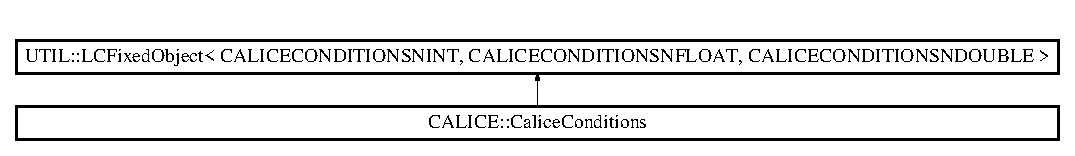
\includegraphics[height=1.647059cm]{classCALICE_1_1CaliceConditions}
\end{center}
\end{figure}
\subsection*{Public Member Functions}
\begin{DoxyCompactItemize}
\item 
{\bf Calice\-Conditions} ()\label{classCALICE_1_1CaliceConditions_a57ce28e582904dcf2ae3fa51b8b79349}

\begin{DoxyCompactList}\small\item\em default constructor \end{DoxyCompactList}\item 
{\bf Calice\-Conditions} (int module\-Nr, unsigned module\-I\-D, int calib\-Start, int calib\-Width, bool calib\-Enable, int hold, int hold\-Width, int multiplex, int vcalib, int verification, int sr[12])
\begin{DoxyCompactList}\small\item\em constructor, Calice\-Condition is initialized with the parameters given \end{DoxyCompactList}\item 
{\bfseries Calice\-Conditions} (L\-C\-Object $\ast$obj)\label{classCALICE_1_1CaliceConditions_a9ff7c93b1ed0d3a138591cf301bf75d8}

\item 
unsigned {\bf get\-Module\-I\-D} () const \label{classCALICE_1_1CaliceConditions_aedaf26b7d1fb15c363c850f1f8c82b4c}

\begin{DoxyCompactList}\small\item\em get module I\-D of config \end{DoxyCompactList}\item 
unsigned {\bf get\-Module\-Nr} ()\label{classCALICE_1_1CaliceConditions_aff3abefa487659e235d319026855e0da}

\begin{DoxyCompactList}\small\item\em get module number of config \end{DoxyCompactList}\item 
unsigned {\bf get\-Calib\-Start} () const \label{classCALICE_1_1CaliceConditions_a63e3e50d28697586dba6649d23f09e86}

\begin{DoxyCompactList}\small\item\em get calib start \end{DoxyCompactList}\item 
unsigned {\bf get\-Calib\-Width} () const \label{classCALICE_1_1CaliceConditions_ab8dd4e2da8c51aab6c2f2f2b5c297697}

\begin{DoxyCompactList}\small\item\em get calib width \end{DoxyCompactList}\item 
bool {\bf is\-Calib\-Enabled} () const \label{classCALICE_1_1CaliceConditions_afe4ca5760e990760a959fd4ed47fbd9c}

\begin{DoxyCompactList}\small\item\em get if calib is enabled \end{DoxyCompactList}\item 
float {\bf get\-Hold} () const \label{classCALICE_1_1CaliceConditions_a55a69a52404fd1bc77991052db53ff8d}

\begin{DoxyCompactList}\small\item\em get hold \end{DoxyCompactList}\item 
unsigned {\bf get\-Hold\-Width} () const \label{classCALICE_1_1CaliceConditions_a2898d9c3cea46e646016d31423cc2208}

\begin{DoxyCompactList}\small\item\em get hold width \end{DoxyCompactList}\item 
unsigned {\bf get\-Multiplex} () const \label{classCALICE_1_1CaliceConditions_a748f60dfba34117e777cef4f479b3ae1}

\begin{DoxyCompactList}\small\item\em get order of multiplexing \end{DoxyCompactList}\item 
unsigned {\bf get\-Vcalib} () const \label{classCALICE_1_1CaliceConditions_a23a06d3340b909f021778df6c42f3572}

\begin{DoxyCompactList}\small\item\em get vcalib \end{DoxyCompactList}\item 
unsigned {\bf get\-Verification} () const \label{classCALICE_1_1CaliceConditions_a930fac5aac0b5e5f5e0d535144d9cb0b}

\begin{DoxyCompactList}\small\item\em get verification data \end{DoxyCompactList}\item 
unsigned {\bf get\-S\-R} (unsigned hab) const \label{classCALICE_1_1CaliceConditions_a7146de11fbfc7f531048ef41e7ea7ccf}

\begin{DoxyCompactList}\small\item\em get hab sr \end{DoxyCompactList}\item 
void {\bf print} (std\-::ostream \&os)\label{classCALICE_1_1CaliceConditions_aedb71bf9e2871d727c1dbb7828571639}

\begin{DoxyCompactList}\small\item\em convenient print method \end{DoxyCompactList}\item 
const std\-::string {\bf get\-Type\-Name} () const \label{classCALICE_1_1CaliceConditions_adc16043084a7beaff71c3b76a6ad6ac1}

\begin{DoxyCompactList}\small\item\em return the type of the class \end{DoxyCompactList}\item 
const std\-::string {\bf get\-Data\-Description} () const \label{classCALICE_1_1CaliceConditions_ae854b2d852e1c484246bf45544da38ae}

\begin{DoxyCompactList}\small\item\em return a brief description of the data memeber \end{DoxyCompactList}\end{DoxyCompactItemize}


\subsection{Detailed Description}
Class for the \doxyref{C\-A\-L\-I\-C\-E}{p.}{namespaceCALICE} Ahcal conditions information during the reconstruction. 

Information is stored module wise \begin{DoxyAuthor}{Author}
B. Lutz D\-E\-S\-Y 
\end{DoxyAuthor}
\begin{DoxyDate}{Date}
Sep 11 2006 
\end{DoxyDate}


Definition at line 30 of file Calice\-Conditions.\-hh.



\subsection{Constructor \& Destructor Documentation}
\index{C\-A\-L\-I\-C\-E\-::\-Calice\-Conditions@{C\-A\-L\-I\-C\-E\-::\-Calice\-Conditions}!Calice\-Conditions@{Calice\-Conditions}}
\index{Calice\-Conditions@{Calice\-Conditions}!CALICE::CaliceConditions@{C\-A\-L\-I\-C\-E\-::\-Calice\-Conditions}}
\subsubsection[{Calice\-Conditions}]{\setlength{\rightskip}{0pt plus 5cm}C\-A\-L\-I\-C\-E\-::\-Calice\-Conditions\-::\-Calice\-Conditions (
\begin{DoxyParamCaption}
\item[{int}]{module\-Nr, }
\item[{unsigned}]{module\-I\-D, }
\item[{int}]{calib\-Start, }
\item[{int}]{calib\-Width, }
\item[{bool}]{calib\-Enable, }
\item[{int}]{hold, }
\item[{int}]{hold\-Width, }
\item[{int}]{multiplex, }
\item[{int}]{vcalib, }
\item[{int}]{verification, }
\item[{int}]{sr[12]}
\end{DoxyParamCaption}
)\hspace{0.3cm}{\ttfamily [inline]}}\label{classCALICE_1_1CaliceConditions_ad200640ef3e522d130e97c0982be7410}


constructor, Calice\-Condition is initialized with the parameters given 


\begin{DoxyParams}{Parameters}
{\em module\-Nr} & mdoule \char`\"{}stamp\char`\"{} \\
\hline
{\em module\-I\-D} & module I\-D of the module the hit is in, low byte gives upper or lower half, high byte gives module \char`\"{}stamp\char`\"{}, used to find correct calibration \\
\hline
{\em calib\-Start} & starting time of Tcalib signal in ticks \\
\hline
{\em calib\-Width} & duration of the Tcalib signal in ticks \\
\hline
{\em calib\-Enable} & has Tcalib signal been sent at all? \\
\hline
{\em hold} & starting time of the hold signal in ticks (6.\-25ns) \\
\hline
{\em hold\-Width} & duration of the hold signal in ticks (6.\-25ns) \\
\hline
{\em multiplex} & number of multiplexed signals in the acquisition cycle \\
\hline
{\em vcalib} & Vcalib value \\
\hline
{\em verification} & shift register verification pattern \\
\hline
{\em sr} & shift registers \\
\hline
\end{DoxyParams}


Definition at line 52 of file Calice\-Conditions.\-hh.



The documentation for this class was generated from the following files\-:\begin{DoxyCompactItemize}
\item 
Calice\-Conditions.\-hh\item 
Calice\-Conditions.\-cc\end{DoxyCompactItemize}

\section{C\-A\-L\-I\-C\-E\-:\-:Calice\-Elog\-Info Class Reference}
\label{classCALICE_1_1CaliceElogInfo}\index{C\-A\-L\-I\-C\-E\-::\-Calice\-Elog\-Info@{C\-A\-L\-I\-C\-E\-::\-Calice\-Elog\-Info}}


Implementation of the e-\/log information.  




{\ttfamily \#include $<$Calice\-Elog\-Info.\-hh$>$}

Inheritance diagram for C\-A\-L\-I\-C\-E\-:\-:Calice\-Elog\-Info\-:\begin{figure}[H]
\begin{center}
\leavevmode
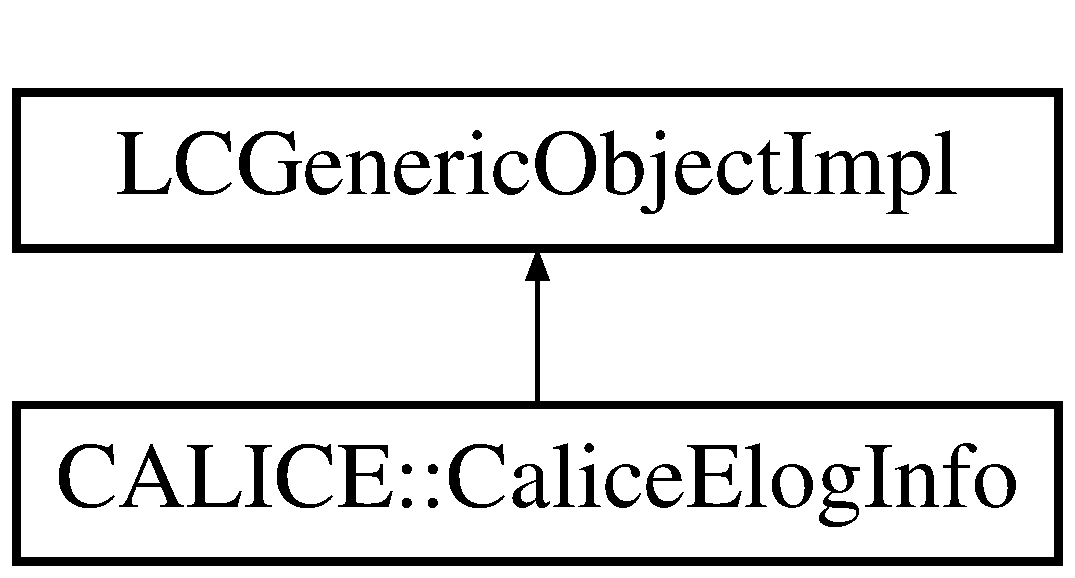
\includegraphics[height=2.000000cm]{classCALICE_1_1CaliceElogInfo}
\end{center}
\end{figure}
\subsection*{Public Member Functions}
\begin{DoxyCompactItemize}
\item 
{\bf Calice\-Elog\-Info} (E\-V\-E\-N\-T\-::\-L\-C\-Collection $\ast$col)
\begin{DoxyCompactList}\small\item\em constructor from L\-C\-Collection (this way, the user does not need to cast anymore) \end{DoxyCompactList}\item 
{\bf Calice\-Elog\-Info} (const unsigned int run\-Number, const int pdg\-Type, const float energy, const int quality\-Flag, const int trigger\-Type, const int trigger\-Setting, const float cherenkov\-Pressure, const float cherenkov2\-Pressure, const float position\-X, const float position\-Y, const float rotation\-Angle)
\begin{DoxyCompactList}\small\item\em constructor from elements \end{DoxyCompactList}\item 
void {\bf set\-Run\-Number} (const unsigned int run\-Number)
\begin{DoxyCompactList}\small\item\em Set the run number. \end{DoxyCompactList}\item 
unsigned int {\bf get\-Run\-Number} ()
\begin{DoxyCompactList}\small\item\em Get the run number. \end{DoxyCompactList}\item 
void {\bf set\-Pdg\-Type} (const int pdg\-Type)
\begin{DoxyCompactList}\small\item\em Set the P\-D\-G I\-D. \end{DoxyCompactList}\item 
int {\bf get\-Pdg\-Type} ()
\begin{DoxyCompactList}\small\item\em Get the P\-D\-G I\-D. \end{DoxyCompactList}\item 
void {\bf set\-Trigger\-Type} (const int trigger\-Type)
\begin{DoxyCompactList}\small\item\em Set the trigger type. \end{DoxyCompactList}\item 
int {\bf get\-Trigger\-Type} ()
\begin{DoxyCompactList}\small\item\em Get the trigger type. \end{DoxyCompactList}\item 
void {\bf set\-Trigger\-Setting} (const int trigger\-Setting)
\begin{DoxyCompactList}\small\item\em Set the trigger setting. \end{DoxyCompactList}\item 
int {\bf get\-Trigger\-Setting} ()
\begin{DoxyCompactList}\small\item\em Get the trigger setting. \end{DoxyCompactList}\item 
void {\bf set\-Quality\-Flag} (const int quality\-Flag)
\begin{DoxyCompactList}\small\item\em Set the quality flag (0=good, 1=bad). \end{DoxyCompactList}\item 
int {\bf get\-Quality\-Flag} ()
\begin{DoxyCompactList}\small\item\em Get the quality flag. \end{DoxyCompactList}\item 
void {\bf set\-Energy} (const float energy)
\begin{DoxyCompactList}\small\item\em Set the energy of this run. \end{DoxyCompactList}\item 
float {\bf get\-Energy} ()
\begin{DoxyCompactList}\small\item\em Get the energy of this run. \end{DoxyCompactList}\item 
void {\bf set\-Cherenkov\-Pressure} (const float cherenkov\-Pressure)
\begin{DoxyCompactList}\small\item\em Set the pressure in Cherenkov counter A. \end{DoxyCompactList}\item 
float {\bf get\-Cherenkov\-Pressure} ()
\begin{DoxyCompactList}\small\item\em Get the pressure in Cherenkov counter A. \end{DoxyCompactList}\item 
void {\bf set\-Cherenkov2\-Pressure} (const float cherenkov2\-Pressure)
\begin{DoxyCompactList}\small\item\em Set the pressure in Cherenkov counter B. \end{DoxyCompactList}\item 
float {\bf get\-Cherenkov2\-Pressure} ()
\begin{DoxyCompactList}\small\item\em Get the pressure in Cherenkov counter B. \end{DoxyCompactList}\item 
void {\bf set\-Position\-X} (const float position\-X)
\begin{DoxyCompactList}\small\item\em Set the x-\/position of the stage. \end{DoxyCompactList}\item 
float {\bf get\-Position\-X} ()
\begin{DoxyCompactList}\small\item\em Get the x-\/position of the stage. \end{DoxyCompactList}\item 
void {\bf set\-Position\-Y} (const float position\-Y)
\begin{DoxyCompactList}\small\item\em Set the y-\/position of the stage. \end{DoxyCompactList}\item 
float {\bf get\-Position\-Y} ()
\begin{DoxyCompactList}\small\item\em Get the y-\/position of the stage. \end{DoxyCompactList}\item 
void {\bf set\-Rotation\-Angle} (const float rotation\-Angle)
\begin{DoxyCompactList}\small\item\em Set the rotation angle of the stage. \end{DoxyCompactList}\item 
float {\bf get\-Rotation\-Angle} ()
\begin{DoxyCompactList}\small\item\em Get the rotation angle of the stage. \end{DoxyCompactList}\item 
void {\bf set\-Run\-Type} (const std\-::string run\-Type)
\begin{DoxyCompactList}\small\item\em Set the run type (beam\-Data, calibration etc) \end{DoxyCompactList}\item 
const std\-::string {\bf get\-Run\-Type} ()\label{classCALICE_1_1CaliceElogInfo_a38072c9af25952630e41d98d0c001512}

\begin{DoxyCompactList}\small\item\em Get the run type (beam\-Data, calibration etc) \end{DoxyCompactList}\item 
void {\bf set\-Target\-String} (const std\-::string target\-String)
\begin{DoxyCompactList}\small\item\em Set the target string. \end{DoxyCompactList}\item 
const std\-::string {\bf get\-Target\-String} (const E\-V\-E\-N\-T\-::\-L\-C\-Parameters \&params)\label{classCALICE_1_1CaliceElogInfo_ab036592fded5b7cf6eef2b905bd8a602}

\begin{DoxyCompactList}\small\item\em Get the target string. \end{DoxyCompactList}\item 
void {\bf set\-Absorber\-String} (const std\-::string absorber\-String)
\begin{DoxyCompactList}\small\item\em Set the absorber string. \end{DoxyCompactList}\item 
const std\-::string {\bf get\-Absorber\-String} (const E\-V\-E\-N\-T\-::\-L\-C\-Parameters \&params)\label{classCALICE_1_1CaliceElogInfo_aeeb0758e7f2491bd15665de2e09d2408}

\begin{DoxyCompactList}\small\item\em Get the absorber string. \end{DoxyCompactList}\item 
void {\bf set\-Comment} (const std\-::string comment)
\begin{DoxyCompactList}\small\item\em Set the comment. \end{DoxyCompactList}\item 
const std\-::string {\bf get\-Comment} (const E\-V\-E\-N\-T\-::\-L\-C\-Parameters \&params)
\begin{DoxyCompactList}\small\item\em Get the comment from the e-\/log. \end{DoxyCompactList}\item 
const std\-::string {\bf get\-Type\-Name} () const 
\begin{DoxyCompactList}\small\item\em Implementation of the virtual method from L\-C\-Generic\-Object. \end{DoxyCompactList}\item 
const std\-::string {\bf get\-Data\-Description} () const 
\begin{DoxyCompactList}\small\item\em Implementation of the virtual method from L\-C\-Generic\-Object. \end{DoxyCompactList}\item 
E\-V\-E\-N\-T\-::\-L\-C\-Collection $\ast$ {\bf get\-Collection} () const \label{classCALICE_1_1CaliceElogInfo_a48625b8367f9c424f9064a8231556ad2}

\begin{DoxyCompactList}\small\item\em Get the L\-C\-Collection. \end{DoxyCompactList}\end{DoxyCompactItemize}
\subsection*{Private Types}
\begin{DoxyCompactItemize}
\item 
enum {\bfseries Ints} \{ \\*
{\bfseries k\-Run\-Number}, 
{\bfseries k\-Pdg\-Type}, 
{\bfseries k\-Quality\-Flag}, 
{\bfseries k\-Trigger\-Type}, 
\\*
{\bfseries k\-Trigger\-Setting}, 
{\bfseries k\-N\-Ints}
 \}
\item 
enum {\bfseries Floats} \{ \\*
{\bfseries k\-Energy}, 
{\bfseries k\-Cherenkov\-Pressure}, 
{\bfseries k\-Cherenkov2\-Pressure}, 
{\bfseries k\-Position\-X}, 
\\*
{\bfseries k\-Position\-Y}, 
{\bfseries k\-Rotation\-Angle}, 
{\bfseries k\-N\-Floats}
 \}
\item 
enum {\bfseries Doubless} \{ {\bfseries k\-N\-Doubles}
 \}
\end{DoxyCompactItemize}
\subsection*{Private Attributes}
\begin{DoxyCompactItemize}
\item 
std\-::string {\bf \-\_\-run\-Type}
\begin{DoxyCompactList}\small\item\em run type, e.\-g. \end{DoxyCompactList}\item 
std\-::string {\bf \-\_\-target\-String}
\begin{DoxyCompactList}\small\item\em target string, e.\-g. \end{DoxyCompactList}\item 
std\-::string {\bf \-\_\-absorber\-String}
\begin{DoxyCompactList}\small\item\em absorber string, e.\-g. \end{DoxyCompactList}\item 
std\-::string {\bf \-\_\-comment}
\begin{DoxyCompactList}\small\item\em e-\/log comment, e.\-g. \end{DoxyCompactList}\end{DoxyCompactItemize}


\subsection{Detailed Description}
Implementation of the e-\/log information. 

\begin{DoxyAuthor}{Author}
{\tt lucaci@mail.\-desy.\-de} 
\end{DoxyAuthor}
\begin{DoxyDate}{Date}
June 2010 
\end{DoxyDate}


Definition at line 18 of file Calice\-Elog\-Info.\-hh.



\subsection{Constructor \& Destructor Documentation}
\index{C\-A\-L\-I\-C\-E\-::\-Calice\-Elog\-Info@{C\-A\-L\-I\-C\-E\-::\-Calice\-Elog\-Info}!Calice\-Elog\-Info@{Calice\-Elog\-Info}}
\index{Calice\-Elog\-Info@{Calice\-Elog\-Info}!CALICE::CaliceElogInfo@{C\-A\-L\-I\-C\-E\-::\-Calice\-Elog\-Info}}
\subsubsection[{Calice\-Elog\-Info}]{\setlength{\rightskip}{0pt plus 5cm}C\-A\-L\-I\-C\-E\-::\-Calice\-Elog\-Info\-::\-Calice\-Elog\-Info (
\begin{DoxyParamCaption}
\item[{E\-V\-E\-N\-T\-::\-L\-C\-Collection $\ast$}]{col}
\end{DoxyParamCaption}
)}\label{classCALICE_1_1CaliceElogInfo_ac95c7a4917689baa38e2d8001f8555b5}


constructor from L\-C\-Collection (this way, the user does not need to cast anymore) 

Constructor from L\-C\-Object\-: use L\-C\-Object, and do the cast from the L\-C\-Generic\-Object; this way, the users do not have to do the cast anymore. 

Definition at line 13 of file Calice\-Elog\-Info.\-cc.



References \-\_\-run\-Type, set\-Cherenkov2\-Pressure(), set\-Cherenkov\-Pressure(), set\-Energy(), set\-Pdg\-Type(), set\-Position\-X(), set\-Position\-Y(), set\-Quality\-Flag(), set\-Rotation\-Angle(), set\-Run\-Number(), set\-Trigger\-Setting(), and set\-Trigger\-Type().

\index{C\-A\-L\-I\-C\-E\-::\-Calice\-Elog\-Info@{C\-A\-L\-I\-C\-E\-::\-Calice\-Elog\-Info}!Calice\-Elog\-Info@{Calice\-Elog\-Info}}
\index{Calice\-Elog\-Info@{Calice\-Elog\-Info}!CALICE::CaliceElogInfo@{C\-A\-L\-I\-C\-E\-::\-Calice\-Elog\-Info}}
\subsubsection[{Calice\-Elog\-Info}]{\setlength{\rightskip}{0pt plus 5cm}C\-A\-L\-I\-C\-E\-::\-Calice\-Elog\-Info\-::\-Calice\-Elog\-Info (
\begin{DoxyParamCaption}
\item[{const unsigned int}]{run\-Number, }
\item[{const int}]{pdg\-Type, }
\item[{const float}]{energy, }
\item[{const int}]{quality\-Flag, }
\item[{const int}]{trigger\-Type, }
\item[{const int}]{trigger\-Setting, }
\item[{const float}]{cherenkov\-Pressure, }
\item[{const float}]{cherenkov2\-Pressure, }
\item[{const float}]{position\-X, }
\item[{const float}]{position\-Y, }
\item[{const float}]{rotation\-Angle}
\end{DoxyParamCaption}
)}\label{classCALICE_1_1CaliceElogInfo_af86284759774e0975c59eef4eb3164cf}


constructor from elements 


\begin{DoxyParams}{Parameters}
{\em run\-Number} & run number \\
\hline
{\em pdg\-Type} & P\-D\-G I\-D of the beam particle (e.\-g. -\/211 for pi-\/) \\
\hline
{\em energy} & energy of the run, in Ge\-V (according to elog information) \\
\hline
{\em quality\-Flag} & quality Flag\-: 0 = good, 1 = junk or garbage \\
\hline
{\em trigger\-Type} & trigger type\-: 10 for the '10x10' trigger, 20 for the '20x20' trigger, 100 for the '100x100' trigger \\
\hline
{\em trigger\-Setting} & trigger setting (available only for F\-N\-A\-L data, see elog) \\
\hline
{\em cherenkov\-Pressure} & pressure in cherenkov counter A, in psia \\
\hline
{\em cherenkov2\-Pressure} & pressure in cherenkov counter B, in psia \\
\hline
{\em position\-X} & x position of the beam, in mm \\
\hline
{\em position\-Y} & y position of the beam, in mm \\
\hline
{\em rotation\-Angle} & rotation angle (in degrees) \\
\hline
\end{DoxyParams}


\subsection{Member Function Documentation}
\index{C\-A\-L\-I\-C\-E\-::\-Calice\-Elog\-Info@{C\-A\-L\-I\-C\-E\-::\-Calice\-Elog\-Info}!get\-Cherenkov2\-Pressure@{get\-Cherenkov2\-Pressure}}
\index{get\-Cherenkov2\-Pressure@{get\-Cherenkov2\-Pressure}!CALICE::CaliceElogInfo@{C\-A\-L\-I\-C\-E\-::\-Calice\-Elog\-Info}}
\subsubsection[{get\-Cherenkov2\-Pressure}]{\setlength{\rightskip}{0pt plus 5cm}float C\-A\-L\-I\-C\-E\-::\-Calice\-Elog\-Info\-::get\-Cherenkov2\-Pressure (
\begin{DoxyParamCaption}
{}
\end{DoxyParamCaption}
)}\label{classCALICE_1_1CaliceElogInfo_a70529642b2e5e744993d851a2d4d5a35}


Get the pressure in Cherenkov counter B. 

\begin{DoxyReturn}{Returns}
the Cherenkov pressure 
\end{DoxyReturn}


Definition at line 162 of file Calice\-Elog\-Info.\-cc.

\index{C\-A\-L\-I\-C\-E\-::\-Calice\-Elog\-Info@{C\-A\-L\-I\-C\-E\-::\-Calice\-Elog\-Info}!get\-Cherenkov\-Pressure@{get\-Cherenkov\-Pressure}}
\index{get\-Cherenkov\-Pressure@{get\-Cherenkov\-Pressure}!CALICE::CaliceElogInfo@{C\-A\-L\-I\-C\-E\-::\-Calice\-Elog\-Info}}
\subsubsection[{get\-Cherenkov\-Pressure}]{\setlength{\rightskip}{0pt plus 5cm}float C\-A\-L\-I\-C\-E\-::\-Calice\-Elog\-Info\-::get\-Cherenkov\-Pressure (
\begin{DoxyParamCaption}
{}
\end{DoxyParamCaption}
)}\label{classCALICE_1_1CaliceElogInfo_a64dba0c7ea6009be1c833d44661a0ebf}


Get the pressure in Cherenkov counter A. 

\begin{DoxyReturn}{Returns}
the Cherenkov pressure 
\end{DoxyReturn}


Definition at line 151 of file Calice\-Elog\-Info.\-cc.

\index{C\-A\-L\-I\-C\-E\-::\-Calice\-Elog\-Info@{C\-A\-L\-I\-C\-E\-::\-Calice\-Elog\-Info}!get\-Comment@{get\-Comment}}
\index{get\-Comment@{get\-Comment}!CALICE::CaliceElogInfo@{C\-A\-L\-I\-C\-E\-::\-Calice\-Elog\-Info}}
\subsubsection[{get\-Comment}]{\setlength{\rightskip}{0pt plus 5cm}const std\-::string C\-A\-L\-I\-C\-E\-::\-Calice\-Elog\-Info\-::get\-Comment (
\begin{DoxyParamCaption}
\item[{const E\-V\-E\-N\-T\-::\-L\-C\-Parameters \&}]{params}
\end{DoxyParamCaption}
)}\label{classCALICE_1_1CaliceElogInfo_a5d7a81f00bdb9ab9260d11416e2ee266}


Get the comment from the e-\/log. 


\begin{DoxyParams}{Parameters}
{\em params} & the L\-C\-Parameters (since the comment is saved as a parameter of the collection of \doxyref{Calice\-Elog\-Info}{p.}{classCALICE_1_1CaliceElogInfo} objects) \\
\hline
\end{DoxyParams}


Definition at line 239 of file Calice\-Elog\-Info.\-cc.

\index{C\-A\-L\-I\-C\-E\-::\-Calice\-Elog\-Info@{C\-A\-L\-I\-C\-E\-::\-Calice\-Elog\-Info}!get\-Data\-Description@{get\-Data\-Description}}
\index{get\-Data\-Description@{get\-Data\-Description}!CALICE::CaliceElogInfo@{C\-A\-L\-I\-C\-E\-::\-Calice\-Elog\-Info}}
\subsubsection[{get\-Data\-Description}]{\setlength{\rightskip}{0pt plus 5cm}const std\-::string C\-A\-L\-I\-C\-E\-::\-Calice\-Elog\-Info\-::get\-Data\-Description (
\begin{DoxyParamCaption}
{}
\end{DoxyParamCaption}
) const}\label{classCALICE_1_1CaliceElogInfo_ad2f4fb5b358f25ba0ff59bb4cacadef9}


Implementation of the virtual method from L\-C\-Generic\-Object. 

\begin{DoxyReturn}{Returns}
data description, i.\-e description of the L\-C\-Object elements\-: \char`\"{}i\-:run\-Number,i\-:pdg\-Type,i\-:energy,i\-:quality\-Flag,i\-:trigger\-Type,i\-:trigget\-Setting,\char`\"{} \char`\"{}f\-:cherenkov\-Pressure,f\-:position\-X,f\-:position\-Y,f\-:rotation\-Angle\char`\"{}; 
\end{DoxyReturn}


Definition at line 209 of file Calice\-Elog\-Info.\-cc.

\index{C\-A\-L\-I\-C\-E\-::\-Calice\-Elog\-Info@{C\-A\-L\-I\-C\-E\-::\-Calice\-Elog\-Info}!get\-Energy@{get\-Energy}}
\index{get\-Energy@{get\-Energy}!CALICE::CaliceElogInfo@{C\-A\-L\-I\-C\-E\-::\-Calice\-Elog\-Info}}
\subsubsection[{get\-Energy}]{\setlength{\rightskip}{0pt plus 5cm}float C\-A\-L\-I\-C\-E\-::\-Calice\-Elog\-Info\-::get\-Energy (
\begin{DoxyParamCaption}
{}
\end{DoxyParamCaption}
)}\label{classCALICE_1_1CaliceElogInfo_a7af788f2a7cbda67f1fb37a63fc98271}


Get the energy of this run. 

\begin{DoxyReturn}{Returns}
the energy 
\end{DoxyReturn}


Definition at line 139 of file Calice\-Elog\-Info.\-cc.

\index{C\-A\-L\-I\-C\-E\-::\-Calice\-Elog\-Info@{C\-A\-L\-I\-C\-E\-::\-Calice\-Elog\-Info}!get\-Pdg\-Type@{get\-Pdg\-Type}}
\index{get\-Pdg\-Type@{get\-Pdg\-Type}!CALICE::CaliceElogInfo@{C\-A\-L\-I\-C\-E\-::\-Calice\-Elog\-Info}}
\subsubsection[{get\-Pdg\-Type}]{\setlength{\rightskip}{0pt plus 5cm}int C\-A\-L\-I\-C\-E\-::\-Calice\-Elog\-Info\-::get\-Pdg\-Type (
\begin{DoxyParamCaption}
{}
\end{DoxyParamCaption}
)}\label{classCALICE_1_1CaliceElogInfo_a697ea7426f6177b224da091350b91450}


Get the P\-D\-G I\-D. 

\begin{DoxyReturn}{Returns}
the P\-D\-G I\-D 
\end{DoxyReturn}


Definition at line 90 of file Calice\-Elog\-Info.\-cc.

\index{C\-A\-L\-I\-C\-E\-::\-Calice\-Elog\-Info@{C\-A\-L\-I\-C\-E\-::\-Calice\-Elog\-Info}!get\-Position\-X@{get\-Position\-X}}
\index{get\-Position\-X@{get\-Position\-X}!CALICE::CaliceElogInfo@{C\-A\-L\-I\-C\-E\-::\-Calice\-Elog\-Info}}
\subsubsection[{get\-Position\-X}]{\setlength{\rightskip}{0pt plus 5cm}float C\-A\-L\-I\-C\-E\-::\-Calice\-Elog\-Info\-::get\-Position\-X (
\begin{DoxyParamCaption}
{}
\end{DoxyParamCaption}
)}\label{classCALICE_1_1CaliceElogInfo_a10fbaa90ae11969de35f8cd7c9477c05}


Get the x-\/position of the stage. 

\begin{DoxyReturn}{Returns}
the x-\/position of the stage 
\end{DoxyReturn}


Definition at line 174 of file Calice\-Elog\-Info.\-cc.

\index{C\-A\-L\-I\-C\-E\-::\-Calice\-Elog\-Info@{C\-A\-L\-I\-C\-E\-::\-Calice\-Elog\-Info}!get\-Position\-Y@{get\-Position\-Y}}
\index{get\-Position\-Y@{get\-Position\-Y}!CALICE::CaliceElogInfo@{C\-A\-L\-I\-C\-E\-::\-Calice\-Elog\-Info}}
\subsubsection[{get\-Position\-Y}]{\setlength{\rightskip}{0pt plus 5cm}float C\-A\-L\-I\-C\-E\-::\-Calice\-Elog\-Info\-::get\-Position\-Y (
\begin{DoxyParamCaption}
{}
\end{DoxyParamCaption}
)}\label{classCALICE_1_1CaliceElogInfo_a8567162b99806996bde8ca9d7ba41c05}


Get the y-\/position of the stage. 

\begin{DoxyReturn}{Returns}
the y-\/position of the stage 
\end{DoxyReturn}


Definition at line 185 of file Calice\-Elog\-Info.\-cc.

\index{C\-A\-L\-I\-C\-E\-::\-Calice\-Elog\-Info@{C\-A\-L\-I\-C\-E\-::\-Calice\-Elog\-Info}!get\-Quality\-Flag@{get\-Quality\-Flag}}
\index{get\-Quality\-Flag@{get\-Quality\-Flag}!CALICE::CaliceElogInfo@{C\-A\-L\-I\-C\-E\-::\-Calice\-Elog\-Info}}
\subsubsection[{get\-Quality\-Flag}]{\setlength{\rightskip}{0pt plus 5cm}int C\-A\-L\-I\-C\-E\-::\-Calice\-Elog\-Info\-::get\-Quality\-Flag (
\begin{DoxyParamCaption}
{}
\end{DoxyParamCaption}
)}\label{classCALICE_1_1CaliceElogInfo_a1211b6753b4736c819b163949b645433}


Get the quality flag. 

\begin{DoxyReturn}{Returns}
get the quality flag 
\end{DoxyReturn}


Definition at line 102 of file Calice\-Elog\-Info.\-cc.

\index{C\-A\-L\-I\-C\-E\-::\-Calice\-Elog\-Info@{C\-A\-L\-I\-C\-E\-::\-Calice\-Elog\-Info}!get\-Rotation\-Angle@{get\-Rotation\-Angle}}
\index{get\-Rotation\-Angle@{get\-Rotation\-Angle}!CALICE::CaliceElogInfo@{C\-A\-L\-I\-C\-E\-::\-Calice\-Elog\-Info}}
\subsubsection[{get\-Rotation\-Angle}]{\setlength{\rightskip}{0pt plus 5cm}float C\-A\-L\-I\-C\-E\-::\-Calice\-Elog\-Info\-::get\-Rotation\-Angle (
\begin{DoxyParamCaption}
{}
\end{DoxyParamCaption}
)}\label{classCALICE_1_1CaliceElogInfo_ab366d0ecb73d742195dcc293b88eed4f}


Get the rotation angle of the stage. 

\begin{DoxyReturn}{Returns}
the rotation angle 
\end{DoxyReturn}


Definition at line 197 of file Calice\-Elog\-Info.\-cc.

\index{C\-A\-L\-I\-C\-E\-::\-Calice\-Elog\-Info@{C\-A\-L\-I\-C\-E\-::\-Calice\-Elog\-Info}!get\-Run\-Number@{get\-Run\-Number}}
\index{get\-Run\-Number@{get\-Run\-Number}!CALICE::CaliceElogInfo@{C\-A\-L\-I\-C\-E\-::\-Calice\-Elog\-Info}}
\subsubsection[{get\-Run\-Number}]{\setlength{\rightskip}{0pt plus 5cm}unsigned int C\-A\-L\-I\-C\-E\-::\-Calice\-Elog\-Info\-::get\-Run\-Number (
\begin{DoxyParamCaption}
{}
\end{DoxyParamCaption}
)}\label{classCALICE_1_1CaliceElogInfo_a1f913b1191a57417115181042d61bebb}


Get the run number. 

\begin{DoxyReturn}{Returns}
the run number 
\end{DoxyReturn}


Definition at line 78 of file Calice\-Elog\-Info.\-cc.

\index{C\-A\-L\-I\-C\-E\-::\-Calice\-Elog\-Info@{C\-A\-L\-I\-C\-E\-::\-Calice\-Elog\-Info}!get\-Trigger\-Setting@{get\-Trigger\-Setting}}
\index{get\-Trigger\-Setting@{get\-Trigger\-Setting}!CALICE::CaliceElogInfo@{C\-A\-L\-I\-C\-E\-::\-Calice\-Elog\-Info}}
\subsubsection[{get\-Trigger\-Setting}]{\setlength{\rightskip}{0pt plus 5cm}int C\-A\-L\-I\-C\-E\-::\-Calice\-Elog\-Info\-::get\-Trigger\-Setting (
\begin{DoxyParamCaption}
{}
\end{DoxyParamCaption}
)}\label{classCALICE_1_1CaliceElogInfo_a43bddb9063ee8deb8a99f47ff40f60c5}


Get the trigger setting. 

\begin{DoxyReturn}{Returns}
the trigger setting 
\end{DoxyReturn}


Definition at line 125 of file Calice\-Elog\-Info.\-cc.

\index{C\-A\-L\-I\-C\-E\-::\-Calice\-Elog\-Info@{C\-A\-L\-I\-C\-E\-::\-Calice\-Elog\-Info}!get\-Trigger\-Type@{get\-Trigger\-Type}}
\index{get\-Trigger\-Type@{get\-Trigger\-Type}!CALICE::CaliceElogInfo@{C\-A\-L\-I\-C\-E\-::\-Calice\-Elog\-Info}}
\subsubsection[{get\-Trigger\-Type}]{\setlength{\rightskip}{0pt plus 5cm}int C\-A\-L\-I\-C\-E\-::\-Calice\-Elog\-Info\-::get\-Trigger\-Type (
\begin{DoxyParamCaption}
{}
\end{DoxyParamCaption}
)}\label{classCALICE_1_1CaliceElogInfo_ae69657e00230909eacaa96df61246c36}


Get the trigger type. 

\begin{DoxyReturn}{Returns}
the trigger type (10 for the '10x10' trigger, 20 for the '20x20' trigger, 100 for the '100x100' trigger) 
\end{DoxyReturn}


Definition at line 114 of file Calice\-Elog\-Info.\-cc.

\index{C\-A\-L\-I\-C\-E\-::\-Calice\-Elog\-Info@{C\-A\-L\-I\-C\-E\-::\-Calice\-Elog\-Info}!get\-Type\-Name@{get\-Type\-Name}}
\index{get\-Type\-Name@{get\-Type\-Name}!CALICE::CaliceElogInfo@{C\-A\-L\-I\-C\-E\-::\-Calice\-Elog\-Info}}
\subsubsection[{get\-Type\-Name}]{\setlength{\rightskip}{0pt plus 5cm}const std\-::string C\-A\-L\-I\-C\-E\-::\-Calice\-Elog\-Info\-::get\-Type\-Name (
\begin{DoxyParamCaption}
{}
\end{DoxyParamCaption}
) const}\label{classCALICE_1_1CaliceElogInfo_ac7d8e9cfc726aed8b82184386df1d0f3}


Implementation of the virtual method from L\-C\-Generic\-Object. 

\begin{DoxyReturn}{Returns}
type name, i.\-e. name of the class 
\end{DoxyReturn}


Definition at line 204 of file Calice\-Elog\-Info.\-cc.

\index{C\-A\-L\-I\-C\-E\-::\-Calice\-Elog\-Info@{C\-A\-L\-I\-C\-E\-::\-Calice\-Elog\-Info}!set\-Absorber\-String@{set\-Absorber\-String}}
\index{set\-Absorber\-String@{set\-Absorber\-String}!CALICE::CaliceElogInfo@{C\-A\-L\-I\-C\-E\-::\-Calice\-Elog\-Info}}
\subsubsection[{set\-Absorber\-String}]{\setlength{\rightskip}{0pt plus 5cm}void C\-A\-L\-I\-C\-E\-::\-Calice\-Elog\-Info\-::set\-Absorber\-String (
\begin{DoxyParamCaption}
\item[{const std\-::string}]{absorber\-String}
\end{DoxyParamCaption}
)}\label{classCALICE_1_1CaliceElogInfo_a859927fef587dd3d1ed1ba6fc9a6e59d}


Set the absorber string. 


\begin{DoxyParams}{Parameters}
{\em absorber\-String} & the target string to be set \\
\hline
\end{DoxyParams}
\index{C\-A\-L\-I\-C\-E\-::\-Calice\-Elog\-Info@{C\-A\-L\-I\-C\-E\-::\-Calice\-Elog\-Info}!set\-Cherenkov2\-Pressure@{set\-Cherenkov2\-Pressure}}
\index{set\-Cherenkov2\-Pressure@{set\-Cherenkov2\-Pressure}!CALICE::CaliceElogInfo@{C\-A\-L\-I\-C\-E\-::\-Calice\-Elog\-Info}}
\subsubsection[{set\-Cherenkov2\-Pressure}]{\setlength{\rightskip}{0pt plus 5cm}void C\-A\-L\-I\-C\-E\-::\-Calice\-Elog\-Info\-::set\-Cherenkov2\-Pressure (
\begin{DoxyParamCaption}
\item[{const float}]{cherenkov2\-Pressure}
\end{DoxyParamCaption}
)}\label{classCALICE_1_1CaliceElogInfo_a20ab6bff51831653e7215c72f99e1d07}


Set the pressure in Cherenkov counter B. 


\begin{DoxyParams}{Parameters}
{\em cherenkov2\-Pressure} & the Cherenkov pressure to be set \\
\hline
\end{DoxyParams}


Definition at line 157 of file Calice\-Elog\-Info.\-cc.



Referenced by Calice\-Elog\-Info().

\index{C\-A\-L\-I\-C\-E\-::\-Calice\-Elog\-Info@{C\-A\-L\-I\-C\-E\-::\-Calice\-Elog\-Info}!set\-Cherenkov\-Pressure@{set\-Cherenkov\-Pressure}}
\index{set\-Cherenkov\-Pressure@{set\-Cherenkov\-Pressure}!CALICE::CaliceElogInfo@{C\-A\-L\-I\-C\-E\-::\-Calice\-Elog\-Info}}
\subsubsection[{set\-Cherenkov\-Pressure}]{\setlength{\rightskip}{0pt plus 5cm}void C\-A\-L\-I\-C\-E\-::\-Calice\-Elog\-Info\-::set\-Cherenkov\-Pressure (
\begin{DoxyParamCaption}
\item[{const float}]{cherenkov\-Pressure}
\end{DoxyParamCaption}
)}\label{classCALICE_1_1CaliceElogInfo_afefee1aa0ee343a7b813305826163270}


Set the pressure in Cherenkov counter A. 


\begin{DoxyParams}{Parameters}
{\em cherenkov\-Pressure} & the Cherenkov pressure to be set \\
\hline
\end{DoxyParams}


Definition at line 146 of file Calice\-Elog\-Info.\-cc.



Referenced by Calice\-Elog\-Info().

\index{C\-A\-L\-I\-C\-E\-::\-Calice\-Elog\-Info@{C\-A\-L\-I\-C\-E\-::\-Calice\-Elog\-Info}!set\-Comment@{set\-Comment}}
\index{set\-Comment@{set\-Comment}!CALICE::CaliceElogInfo@{C\-A\-L\-I\-C\-E\-::\-Calice\-Elog\-Info}}
\subsubsection[{set\-Comment}]{\setlength{\rightskip}{0pt plus 5cm}void C\-A\-L\-I\-C\-E\-::\-Calice\-Elog\-Info\-::set\-Comment (
\begin{DoxyParamCaption}
\item[{const std\-::string}]{comment}
\end{DoxyParamCaption}
)}\label{classCALICE_1_1CaliceElogInfo_aa0c8d3a4999b87c62e2a55e7848bd870}


Set the comment. 


\begin{DoxyParams}{Parameters}
{\em comment} & the comment to be set \\
\hline
\end{DoxyParams}
\index{C\-A\-L\-I\-C\-E\-::\-Calice\-Elog\-Info@{C\-A\-L\-I\-C\-E\-::\-Calice\-Elog\-Info}!set\-Energy@{set\-Energy}}
\index{set\-Energy@{set\-Energy}!CALICE::CaliceElogInfo@{C\-A\-L\-I\-C\-E\-::\-Calice\-Elog\-Info}}
\subsubsection[{set\-Energy}]{\setlength{\rightskip}{0pt plus 5cm}void C\-A\-L\-I\-C\-E\-::\-Calice\-Elog\-Info\-::set\-Energy (
\begin{DoxyParamCaption}
\item[{const float}]{energy}
\end{DoxyParamCaption}
)}\label{classCALICE_1_1CaliceElogInfo_af19688a789197c84db6273d606ce0a3f}


Set the energy of this run. 


\begin{DoxyParams}{Parameters}
{\em energy} & the energy to be set \\
\hline
\end{DoxyParams}


Definition at line 134 of file Calice\-Elog\-Info.\-cc.



Referenced by Calice\-Elog\-Info().

\index{C\-A\-L\-I\-C\-E\-::\-Calice\-Elog\-Info@{C\-A\-L\-I\-C\-E\-::\-Calice\-Elog\-Info}!set\-Pdg\-Type@{set\-Pdg\-Type}}
\index{set\-Pdg\-Type@{set\-Pdg\-Type}!CALICE::CaliceElogInfo@{C\-A\-L\-I\-C\-E\-::\-Calice\-Elog\-Info}}
\subsubsection[{set\-Pdg\-Type}]{\setlength{\rightskip}{0pt plus 5cm}void C\-A\-L\-I\-C\-E\-::\-Calice\-Elog\-Info\-::set\-Pdg\-Type (
\begin{DoxyParamCaption}
\item[{const int}]{pdg\-Type}
\end{DoxyParamCaption}
)}\label{classCALICE_1_1CaliceElogInfo_a90bdb26738e9e5343af9c034816ef4f5}


Set the P\-D\-G I\-D. 


\begin{DoxyParams}{Parameters}
{\em pdg\-Type} & P\-D\-G I\-D to be set \\
\hline
\end{DoxyParams}


Definition at line 85 of file Calice\-Elog\-Info.\-cc.



Referenced by Calice\-Elog\-Info().

\index{C\-A\-L\-I\-C\-E\-::\-Calice\-Elog\-Info@{C\-A\-L\-I\-C\-E\-::\-Calice\-Elog\-Info}!set\-Position\-X@{set\-Position\-X}}
\index{set\-Position\-X@{set\-Position\-X}!CALICE::CaliceElogInfo@{C\-A\-L\-I\-C\-E\-::\-Calice\-Elog\-Info}}
\subsubsection[{set\-Position\-X}]{\setlength{\rightskip}{0pt plus 5cm}void C\-A\-L\-I\-C\-E\-::\-Calice\-Elog\-Info\-::set\-Position\-X (
\begin{DoxyParamCaption}
\item[{const float}]{position\-X}
\end{DoxyParamCaption}
)}\label{classCALICE_1_1CaliceElogInfo_a3b2cde809cdf5754e5572db98faa1fbd}


Set the x-\/position of the stage. 


\begin{DoxyParams}{Parameters}
{\em position\-X} & the x-\/position of the stage \\
\hline
\end{DoxyParams}


Definition at line 169 of file Calice\-Elog\-Info.\-cc.



Referenced by Calice\-Elog\-Info().

\index{C\-A\-L\-I\-C\-E\-::\-Calice\-Elog\-Info@{C\-A\-L\-I\-C\-E\-::\-Calice\-Elog\-Info}!set\-Position\-Y@{set\-Position\-Y}}
\index{set\-Position\-Y@{set\-Position\-Y}!CALICE::CaliceElogInfo@{C\-A\-L\-I\-C\-E\-::\-Calice\-Elog\-Info}}
\subsubsection[{set\-Position\-Y}]{\setlength{\rightskip}{0pt plus 5cm}void C\-A\-L\-I\-C\-E\-::\-Calice\-Elog\-Info\-::set\-Position\-Y (
\begin{DoxyParamCaption}
\item[{const float}]{position\-Y}
\end{DoxyParamCaption}
)}\label{classCALICE_1_1CaliceElogInfo_ad3c17fc4e4374c18720b4a46ad5d2b66}


Set the y-\/position of the stage. 


\begin{DoxyParams}{Parameters}
{\em position\-Y} & the y-\/position of the stage \\
\hline
\end{DoxyParams}


Definition at line 180 of file Calice\-Elog\-Info.\-cc.



Referenced by Calice\-Elog\-Info().

\index{C\-A\-L\-I\-C\-E\-::\-Calice\-Elog\-Info@{C\-A\-L\-I\-C\-E\-::\-Calice\-Elog\-Info}!set\-Quality\-Flag@{set\-Quality\-Flag}}
\index{set\-Quality\-Flag@{set\-Quality\-Flag}!CALICE::CaliceElogInfo@{C\-A\-L\-I\-C\-E\-::\-Calice\-Elog\-Info}}
\subsubsection[{set\-Quality\-Flag}]{\setlength{\rightskip}{0pt plus 5cm}void C\-A\-L\-I\-C\-E\-::\-Calice\-Elog\-Info\-::set\-Quality\-Flag (
\begin{DoxyParamCaption}
\item[{const int}]{quality\-Flag}
\end{DoxyParamCaption}
)}\label{classCALICE_1_1CaliceElogInfo_a556bdeb94e436ec7be3c75687219b77b}


Set the quality flag (0=good, 1=bad). 

Please note that this is a general quality flag, based on the comments done by the people on shift. If they mentioned that the run was 'bad', 'junk' or 'garbage', the quality flag for this run is set to 1 (i.\-e. bad). This is different from the data quality flag set by the D\-Q bits (for more information, please see here\-: {\tt http\-://www-\/flc.\-desy.\-de/flc/flcwiki/\-Run\-Log\-Data\-Quality} 
\begin{DoxyParams}{Parameters}
{\em quality\-Flag} & the quality flag to be set \\
\hline
\end{DoxyParams}


Definition at line 97 of file Calice\-Elog\-Info.\-cc.



Referenced by Calice\-Elog\-Info().

\index{C\-A\-L\-I\-C\-E\-::\-Calice\-Elog\-Info@{C\-A\-L\-I\-C\-E\-::\-Calice\-Elog\-Info}!set\-Rotation\-Angle@{set\-Rotation\-Angle}}
\index{set\-Rotation\-Angle@{set\-Rotation\-Angle}!CALICE::CaliceElogInfo@{C\-A\-L\-I\-C\-E\-::\-Calice\-Elog\-Info}}
\subsubsection[{set\-Rotation\-Angle}]{\setlength{\rightskip}{0pt plus 5cm}void C\-A\-L\-I\-C\-E\-::\-Calice\-Elog\-Info\-::set\-Rotation\-Angle (
\begin{DoxyParamCaption}
\item[{const float}]{rotation\-Angle}
\end{DoxyParamCaption}
)}\label{classCALICE_1_1CaliceElogInfo_a4c54970b6c6e5eda6b4a5d81b760939b}


Set the rotation angle of the stage. 


\begin{DoxyParams}{Parameters}
{\em rotation\-Angle} & the rotation angle \\
\hline
\end{DoxyParams}


Definition at line 192 of file Calice\-Elog\-Info.\-cc.



Referenced by Calice\-Elog\-Info().

\index{C\-A\-L\-I\-C\-E\-::\-Calice\-Elog\-Info@{C\-A\-L\-I\-C\-E\-::\-Calice\-Elog\-Info}!set\-Run\-Number@{set\-Run\-Number}}
\index{set\-Run\-Number@{set\-Run\-Number}!CALICE::CaliceElogInfo@{C\-A\-L\-I\-C\-E\-::\-Calice\-Elog\-Info}}
\subsubsection[{set\-Run\-Number}]{\setlength{\rightskip}{0pt plus 5cm}void C\-A\-L\-I\-C\-E\-::\-Calice\-Elog\-Info\-::set\-Run\-Number (
\begin{DoxyParamCaption}
\item[{const unsigned int}]{run\-Number}
\end{DoxyParamCaption}
)}\label{classCALICE_1_1CaliceElogInfo_a6baaf70dc59575276292de977cac70e5}


Set the run number. 


\begin{DoxyParams}{Parameters}
{\em run\-Number} & the run number to be set \\
\hline
\end{DoxyParams}


Definition at line 73 of file Calice\-Elog\-Info.\-cc.



Referenced by Calice\-Elog\-Info().

\index{C\-A\-L\-I\-C\-E\-::\-Calice\-Elog\-Info@{C\-A\-L\-I\-C\-E\-::\-Calice\-Elog\-Info}!set\-Run\-Type@{set\-Run\-Type}}
\index{set\-Run\-Type@{set\-Run\-Type}!CALICE::CaliceElogInfo@{C\-A\-L\-I\-C\-E\-::\-Calice\-Elog\-Info}}
\subsubsection[{set\-Run\-Type}]{\setlength{\rightskip}{0pt plus 5cm}void C\-A\-L\-I\-C\-E\-::\-Calice\-Elog\-Info\-::set\-Run\-Type (
\begin{DoxyParamCaption}
\item[{const std\-::string}]{run\-Type}
\end{DoxyParamCaption}
)}\label{classCALICE_1_1CaliceElogInfo_aaa477c9f9a50257d116a99cab4883ae2}


Set the run type (beam\-Data, calibration etc) 


\begin{DoxyParams}{Parameters}
{\em run\-Type} & \\
\hline
\end{DoxyParams}


Definition at line 220 of file Calice\-Elog\-Info.\-cc.



References \-\_\-run\-Type.

\index{C\-A\-L\-I\-C\-E\-::\-Calice\-Elog\-Info@{C\-A\-L\-I\-C\-E\-::\-Calice\-Elog\-Info}!set\-Target\-String@{set\-Target\-String}}
\index{set\-Target\-String@{set\-Target\-String}!CALICE::CaliceElogInfo@{C\-A\-L\-I\-C\-E\-::\-Calice\-Elog\-Info}}
\subsubsection[{set\-Target\-String}]{\setlength{\rightskip}{0pt plus 5cm}void C\-A\-L\-I\-C\-E\-::\-Calice\-Elog\-Info\-::set\-Target\-String (
\begin{DoxyParamCaption}
\item[{const std\-::string}]{target\-String}
\end{DoxyParamCaption}
)}\label{classCALICE_1_1CaliceElogInfo_a03b57d4587a38ff31829536580628525}


Set the target string. 


\begin{DoxyParams}{Parameters}
{\em target\-String} & the target string to be set \\
\hline
\end{DoxyParams}
\index{C\-A\-L\-I\-C\-E\-::\-Calice\-Elog\-Info@{C\-A\-L\-I\-C\-E\-::\-Calice\-Elog\-Info}!set\-Trigger\-Setting@{set\-Trigger\-Setting}}
\index{set\-Trigger\-Setting@{set\-Trigger\-Setting}!CALICE::CaliceElogInfo@{C\-A\-L\-I\-C\-E\-::\-Calice\-Elog\-Info}}
\subsubsection[{set\-Trigger\-Setting}]{\setlength{\rightskip}{0pt plus 5cm}void C\-A\-L\-I\-C\-E\-::\-Calice\-Elog\-Info\-::set\-Trigger\-Setting (
\begin{DoxyParamCaption}
\item[{const int}]{trigger\-Setting}
\end{DoxyParamCaption}
)}\label{classCALICE_1_1CaliceElogInfo_a48863237a83d1e4002693ffa07885690}


Set the trigger setting. 


\begin{DoxyParams}{Parameters}
{\em trigger\-Setting} & \\
\hline
\end{DoxyParams}


Definition at line 120 of file Calice\-Elog\-Info.\-cc.



Referenced by Calice\-Elog\-Info().

\index{C\-A\-L\-I\-C\-E\-::\-Calice\-Elog\-Info@{C\-A\-L\-I\-C\-E\-::\-Calice\-Elog\-Info}!set\-Trigger\-Type@{set\-Trigger\-Type}}
\index{set\-Trigger\-Type@{set\-Trigger\-Type}!CALICE::CaliceElogInfo@{C\-A\-L\-I\-C\-E\-::\-Calice\-Elog\-Info}}
\subsubsection[{set\-Trigger\-Type}]{\setlength{\rightskip}{0pt plus 5cm}void C\-A\-L\-I\-C\-E\-::\-Calice\-Elog\-Info\-::set\-Trigger\-Type (
\begin{DoxyParamCaption}
\item[{const int}]{trigger\-Type}
\end{DoxyParamCaption}
)}\label{classCALICE_1_1CaliceElogInfo_afeebb83b902105daab5925dcda2d1c14}


Set the trigger type. 


\begin{DoxyParams}{Parameters}
{\em trigger\-Type} & the trigger type\-: 10 for the '10x10' trigger, 20 for the '20x20' trigger, 100 for the '100x100' trigger \\
\hline
\end{DoxyParams}


Definition at line 109 of file Calice\-Elog\-Info.\-cc.



Referenced by Calice\-Elog\-Info().



\subsection{Field Documentation}
\index{C\-A\-L\-I\-C\-E\-::\-Calice\-Elog\-Info@{C\-A\-L\-I\-C\-E\-::\-Calice\-Elog\-Info}!\-\_\-absorber\-String@{\-\_\-absorber\-String}}
\index{\-\_\-absorber\-String@{\-\_\-absorber\-String}!CALICE::CaliceElogInfo@{C\-A\-L\-I\-C\-E\-::\-Calice\-Elog\-Info}}
\subsubsection[{\-\_\-absorber\-String}]{\setlength{\rightskip}{0pt plus 5cm}std\-::string C\-A\-L\-I\-C\-E\-::\-Calice\-Elog\-Info\-::\-\_\-absorber\-String\hspace{0.3cm}{\ttfamily [private]}}\label{classCALICE_1_1CaliceElogInfo_a6619c62f472cb7385242a0c7d301a1d8}


absorber string, e.\-g. 

\char`\"{}6 mm Pb\char`\"{} 

Definition at line 215 of file Calice\-Elog\-Info.\-hh.

\index{C\-A\-L\-I\-C\-E\-::\-Calice\-Elog\-Info@{C\-A\-L\-I\-C\-E\-::\-Calice\-Elog\-Info}!\-\_\-comment@{\-\_\-comment}}
\index{\-\_\-comment@{\-\_\-comment}!CALICE::CaliceElogInfo@{C\-A\-L\-I\-C\-E\-::\-Calice\-Elog\-Info}}
\subsubsection[{\-\_\-comment}]{\setlength{\rightskip}{0pt plus 5cm}std\-::string C\-A\-L\-I\-C\-E\-::\-Calice\-Elog\-Info\-::\-\_\-comment\hspace{0.3cm}{\ttfamily [private]}}\label{classCALICE_1_1CaliceElogInfo_a5191499169242dc9ad1c43459e6fce51}


e-\/log comment, e.\-g. 

\char`\"{}10 deg, 100k\char`\"{} 

Definition at line 216 of file Calice\-Elog\-Info.\-hh.

\index{C\-A\-L\-I\-C\-E\-::\-Calice\-Elog\-Info@{C\-A\-L\-I\-C\-E\-::\-Calice\-Elog\-Info}!\-\_\-run\-Type@{\-\_\-run\-Type}}
\index{\-\_\-run\-Type@{\-\_\-run\-Type}!CALICE::CaliceElogInfo@{C\-A\-L\-I\-C\-E\-::\-Calice\-Elog\-Info}}
\subsubsection[{\-\_\-run\-Type}]{\setlength{\rightskip}{0pt plus 5cm}std\-::string C\-A\-L\-I\-C\-E\-::\-Calice\-Elog\-Info\-::\-\_\-run\-Type\hspace{0.3cm}{\ttfamily [private]}}\label{classCALICE_1_1CaliceElogInfo_a1a1821d59f676a7805131d53f6310eff}


run type, e.\-g. 

\char`\"{}beam\-Data\char`\"{}, noise, etc 

Definition at line 213 of file Calice\-Elog\-Info.\-hh.



Referenced by Calice\-Elog\-Info(), get\-Collection(), get\-Run\-Type(), and set\-Run\-Type().

\index{C\-A\-L\-I\-C\-E\-::\-Calice\-Elog\-Info@{C\-A\-L\-I\-C\-E\-::\-Calice\-Elog\-Info}!\-\_\-target\-String@{\-\_\-target\-String}}
\index{\-\_\-target\-String@{\-\_\-target\-String}!CALICE::CaliceElogInfo@{C\-A\-L\-I\-C\-E\-::\-Calice\-Elog\-Info}}
\subsubsection[{\-\_\-target\-String}]{\setlength{\rightskip}{0pt plus 5cm}std\-::string C\-A\-L\-I\-C\-E\-::\-Calice\-Elog\-Info\-::\-\_\-target\-String\hspace{0.3cm}{\ttfamily [private]}}\label{classCALICE_1_1CaliceElogInfo_a93c30846719e525039e370d49d420dd0}


target string, e.\-g. 

\char`\"{}air\char`\"{} 

Definition at line 214 of file Calice\-Elog\-Info.\-hh.



The documentation for this class was generated from the following files\-:\begin{DoxyCompactItemize}
\item 
Calice\-Elog\-Info.\-hh\item 
Calice\-Elog\-Info.\-cc\end{DoxyCompactItemize}

\section{C\-A\-L\-I\-C\-E\-:\-:Calice\-Hit Class Reference}
\label{classCALICE_1_1CaliceHit}\index{C\-A\-L\-I\-C\-E\-::\-Calice\-Hit@{C\-A\-L\-I\-C\-E\-::\-Calice\-Hit}}


Class for the \doxyref{C\-A\-L\-I\-C\-E}{p.}{namespaceCALICE} Hcal calorimeter hit information during the reconstruction.  




{\ttfamily \#include $<$Calice\-Hit.\-hh$>$}

Inheritance diagram for C\-A\-L\-I\-C\-E\-:\-:Calice\-Hit\-:\begin{figure}[H]
\begin{center}
\leavevmode
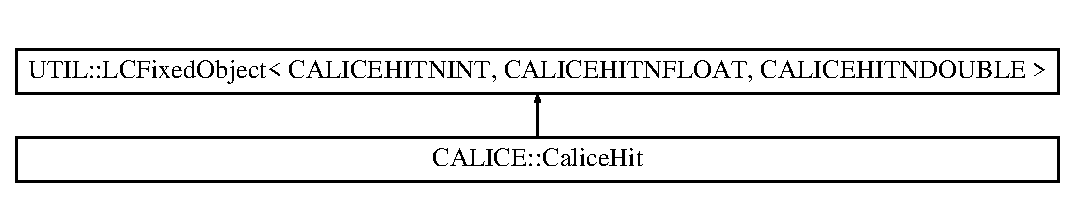
\includegraphics[height=2.000000cm]{classCALICE_1_1CaliceHit}
\end{center}
\end{figure}
\subsection*{Public Member Functions}
\begin{DoxyCompactItemize}
\item 
{\bf Calice\-Hit} ()\label{classCALICE_1_1CaliceHit_a98ecad92603cd9e49ccd8189563c1295}

\begin{DoxyCompactList}\small\item\em default constructor \end{DoxyCompactList}\item 
{\bf Calice\-Hit} (unsigned module\-I\-D, unsigned chip, unsigned channel, float value\-Energy, float error\-Energy, int time\-Stamp, unsigned type)
\begin{DoxyCompactList}\small\item\em constructor, initialise \doxyref{Calice\-Hit}{p.}{classCALICE_1_1CaliceHit} according to parameters \end{DoxyCompactList}\item 
{\bfseries Calice\-Hit} (L\-C\-Object $\ast$obj)\label{classCALICE_1_1CaliceHit_a2581b54e9f99b7fcdb7e96510e7ee08b}

\item 
unsigned {\bf get\-Module\-I\-D} () const \label{classCALICE_1_1CaliceHit_ab9a38707cc073a27926c30565c9ec824}

\begin{DoxyCompactList}\small\item\em get module number of hit \end{DoxyCompactList}\item 
unsigned {\bf get\-Chip} () const \label{classCALICE_1_1CaliceHit_ab6d1980c258c243d66f0e78e5e9cc3ab}

\begin{DoxyCompactList}\small\item\em get chip number of hit \end{DoxyCompactList}\item 
unsigned {\bf get\-Channel} () const \label{classCALICE_1_1CaliceHit_aa204afaa3c519bb2e1ede393fcb071a6}

\begin{DoxyCompactList}\small\item\em get channel number of hit \end{DoxyCompactList}\item 
unsigned {\bf get\-Cell\-Key} () const \label{classCALICE_1_1CaliceHit_a17eacb1d5795af85c01636784185e457}

\begin{DoxyCompactList}\small\item\em get cell\-Key \end{DoxyCompactList}\item 
float {\bf get\-Energy\-Value} () const \label{classCALICE_1_1CaliceHit_ab88be7f3019bee7021d98e6e36bb0e5e}

\begin{DoxyCompactList}\small\item\em get energy value of hit \end{DoxyCompactList}\item 
float {\bf get\-Energy\-Error} () const \label{classCALICE_1_1CaliceHit_a36f21345ae212fca7b7fcc51a1620f2d}

\begin{DoxyCompactList}\small\item\em get energy error of hit \end{DoxyCompactList}\item 
int {\bf get\-Time\-Stamp} () const \label{classCALICE_1_1CaliceHit_a1795a0cec41e5509b39cdc86bccae3ac}

\begin{DoxyCompactList}\small\item\em get time stamp \end{DoxyCompactList}\item 
unsigned {\bf get\-Type} () const \label{classCALICE_1_1CaliceHit_ac30e29cb253ab4c4065606a432c62da9}

\begin{DoxyCompactList}\small\item\em get reconstruction status of hit \end{DoxyCompactList}\item 
void {\bf set\-Energy\-Value} (float energy\-Value)\label{classCALICE_1_1CaliceHit_a2ea22b2f7b0ba157dc379958f99d07e0}

\begin{DoxyCompactList}\small\item\em set energy value of hit \end{DoxyCompactList}\item 
void {\bf set\-Energy\-Error} (float energy\-Error)\label{classCALICE_1_1CaliceHit_aa9ba1721dd909e8723a7af83aee8f57b}

\begin{DoxyCompactList}\small\item\em set energy error of hit \end{DoxyCompactList}\item 
void {\bf set\-Time\-Stamp} (unsigned time\-Stamp)\label{classCALICE_1_1CaliceHit_a9d7c96ae4e6524f98ede0aa9bb35a7d9}

\begin{DoxyCompactList}\small\item\em set time stamp \end{DoxyCompactList}\item 
void {\bf set\-Type} (unsigned type)\label{classCALICE_1_1CaliceHit_af7b49ed9c0ac03cb4877152174022e5a}

\begin{DoxyCompactList}\small\item\em set reconstruction status of hit \end{DoxyCompactList}\item 
void {\bf print} (std\-::ostream \&os)\label{classCALICE_1_1CaliceHit_a327920f1c5d85d67e813b3e5b61c24bf}

\begin{DoxyCompactList}\small\item\em convenient print method \end{DoxyCompactList}\item 
const std\-::string {\bf get\-Type\-Name} () const \label{classCALICE_1_1CaliceHit_ae4b8e7ded0d4c496bc680b69492610e8}

\begin{DoxyCompactList}\small\item\em return the type of the class \end{DoxyCompactList}\item 
const std\-::string {\bf get\-Data\-Description} () const \label{classCALICE_1_1CaliceHit_a973929d198a57c6adbe1912c1ed0fc9c}

\begin{DoxyCompactList}\small\item\em return a brief description of the data memeber \end{DoxyCompactList}\end{DoxyCompactItemize}


\subsection{Detailed Description}
Class for the \doxyref{C\-A\-L\-I\-C\-E}{p.}{namespaceCALICE} Hcal calorimeter hit information during the reconstruction. 

Information is stored module wise (compared to x,y,z position in Calorimeter\-Hits). Energies are stored as float (compared to A\-D\-C counts in Raw\-Calorimeter\-Hits). \begin{DoxyAuthor}{Author}
S. Schmidt D\-E\-S\-Y 
\end{DoxyAuthor}
\begin{DoxyDate}{Date}
Jun 15 2006 
\end{DoxyDate}


Definition at line 28 of file Calice\-Hit.\-hh.



\subsection{Constructor \& Destructor Documentation}
\index{C\-A\-L\-I\-C\-E\-::\-Calice\-Hit@{C\-A\-L\-I\-C\-E\-::\-Calice\-Hit}!Calice\-Hit@{Calice\-Hit}}
\index{Calice\-Hit@{Calice\-Hit}!CALICE::CaliceHit@{C\-A\-L\-I\-C\-E\-::\-Calice\-Hit}}
\subsubsection[{Calice\-Hit}]{\setlength{\rightskip}{0pt plus 5cm}C\-A\-L\-I\-C\-E\-::\-Calice\-Hit\-::\-Calice\-Hit (
\begin{DoxyParamCaption}
\item[{unsigned}]{module\-I\-D, }
\item[{unsigned}]{chip, }
\item[{unsigned}]{channel, }
\item[{float}]{value\-Energy, }
\item[{float}]{error\-Energy, }
\item[{int}]{time\-Stamp, }
\item[{unsigned}]{type}
\end{DoxyParamCaption}
)\hspace{0.3cm}{\ttfamily [inline]}}\label{classCALICE_1_1CaliceHit_ab0d5c66345681f9892c889ce2c97364c}


constructor, initialise \doxyref{Calice\-Hit}{p.}{classCALICE_1_1CaliceHit} according to parameters 


\begin{DoxyParams}{Parameters}
{\em module\-I\-D} & module I\-D of the module the hit is in, low byte gives upper or lower half, high byte gives module \char`\"{}stamp\char`\"{}, used to find correct calibration \\
\hline
{\em chip} & number of the chip the hit is in, used to find correct calibration \\
\hline
{\em channel} & number of the channel the hist is in, used to find correct calibration \\
\hline
{\em value\-Energy} & \char`\"{}energy\char`\"{} property of the hit (also A\-D\-C hits, energy in units of M\-I\-Ps, etc.) \\
\hline
{\em error\-Energy} & error on the \char`\"{}energy\char`\"{} property of the hit \\
\hline
{\em time\-Stamp} & time\-Stamp of the hit \\
\hline
{\em type} & of the hit, can be used to differentiate between different levels of Calice\-Hits (e.\-g. hits with pedestal subtraction, with M\-I\-P calibration, etc.) \\
\hline
\end{DoxyParams}


Definition at line 47 of file Calice\-Hit.\-hh.



The documentation for this class was generated from the following files\-:\begin{DoxyCompactItemize}
\item 
Calice\-Hit.\-hh\item 
Calice\-Hit.\-cc\end{DoxyCompactItemize}

\section{C\-A\-L\-I\-C\-E\-:\-:Cell\-Description Class Reference}
\label{classCALICE_1_1CellDescription}\index{C\-A\-L\-I\-C\-E\-::\-Cell\-Description@{C\-A\-L\-I\-C\-E\-::\-Cell\-Description}}


class to hold data describing calorimeter cells  




{\ttfamily \#include $<$Cell\-Description.\-hh$>$}

\subsection*{Public Member Functions}
\begin{DoxyCompactItemize}
\item 
void {\bf set\-Position} (const float x, const float y, const float z)
\begin{DoxyCompactList}\small\item\em set position (mm) \end{DoxyCompactList}\item 
void {\bf set\-Size} (const float size\-X, const float size\-Y)
\begin{DoxyCompactList}\small\item\em set size (mm) \end{DoxyCompactList}\item 
void {\bf set\-Angle} (const float angle)
\begin{DoxyCompactList}\small\item\em set angle (degree) \end{DoxyCompactList}\item 
float {\bf get\-X} () const 
\item 
float {\bf get\-Y} () const 
\item 
float {\bf get\-Z} () const 
\item 
float {\bf get\-Size\-X} () const 
\item 
float {\bf get\-Size\-Y} () const 
\item 
float {\bf get\-Angle} () const 
\end{DoxyCompactItemize}
\subsection*{Private Attributes}
\begin{DoxyCompactItemize}
\item 
float {\bfseries \-\_\-x}\label{classCALICE_1_1CellDescription_a7fb41b8afeb9685ae79637ec5468d553}

\item 
float {\bfseries \-\_\-y}\label{classCALICE_1_1CellDescription_a26ec9fdc2f9c3f378174e9ac230ab8ea}

\item 
float {\bfseries \-\_\-z}\label{classCALICE_1_1CellDescription_ac47492d24aa6e1a1f690ede7ec761f90}

\item 
float {\bfseries \-\_\-angle}\label{classCALICE_1_1CellDescription_ae7ec071cb586209c1a875aeaf9668832}

\item 
float {\bfseries \-\_\-size\-X}\label{classCALICE_1_1CellDescription_ae44c3d85f32117dff76664abfcf0c670}

\item 
float {\bfseries \-\_\-size\-Y}\label{classCALICE_1_1CellDescription_acd70a2b79f5fc53f0b5c422cab9ae337}

\end{DoxyCompactItemize}


\subsection{Detailed Description}
class to hold data describing calorimeter cells 

\begin{DoxyAuthor}{Author}
{\tt Benjamin.\-Lutz@desy.\-de} 
\end{DoxyAuthor}
\begin{DoxyVersion}{Version}
0.\-1 
\end{DoxyVersion}
\begin{DoxyDate}{Date}
June 2009 
\end{DoxyDate}


Definition at line 13 of file Cell\-Description.\-hh.



\subsection{Member Function Documentation}
\index{C\-A\-L\-I\-C\-E\-::\-Cell\-Description@{C\-A\-L\-I\-C\-E\-::\-Cell\-Description}!get\-Angle@{get\-Angle}}
\index{get\-Angle@{get\-Angle}!CALICE::CellDescription@{C\-A\-L\-I\-C\-E\-::\-Cell\-Description}}
\subsubsection[{get\-Angle}]{\setlength{\rightskip}{0pt plus 5cm}float C\-A\-L\-I\-C\-E\-::\-Cell\-Description\-::get\-Angle (
\begin{DoxyParamCaption}
{}
\end{DoxyParamCaption}
) const\hspace{0.3cm}{\ttfamily [inline]}}\label{classCALICE_1_1CellDescription_ad8787802904670e475b34ddb3c2ca112}
\begin{DoxyReturn}{Returns}
angle in degree 
\end{DoxyReturn}


Definition at line 73 of file Cell\-Description.\-hh.

\index{C\-A\-L\-I\-C\-E\-::\-Cell\-Description@{C\-A\-L\-I\-C\-E\-::\-Cell\-Description}!get\-Size\-X@{get\-Size\-X}}
\index{get\-Size\-X@{get\-Size\-X}!CALICE::CellDescription@{C\-A\-L\-I\-C\-E\-::\-Cell\-Description}}
\subsubsection[{get\-Size\-X}]{\setlength{\rightskip}{0pt plus 5cm}float C\-A\-L\-I\-C\-E\-::\-Cell\-Description\-::get\-Size\-X (
\begin{DoxyParamCaption}
{}
\end{DoxyParamCaption}
) const\hspace{0.3cm}{\ttfamily [inline]}}\label{classCALICE_1_1CellDescription_ae601ec372a54c912ad9f8f5b419f1d3f}
\begin{DoxyReturn}{Returns}
x-\/size in mm 
\end{DoxyReturn}


Definition at line 64 of file Cell\-Description.\-hh.

\index{C\-A\-L\-I\-C\-E\-::\-Cell\-Description@{C\-A\-L\-I\-C\-E\-::\-Cell\-Description}!get\-Size\-Y@{get\-Size\-Y}}
\index{get\-Size\-Y@{get\-Size\-Y}!CALICE::CellDescription@{C\-A\-L\-I\-C\-E\-::\-Cell\-Description}}
\subsubsection[{get\-Size\-Y}]{\setlength{\rightskip}{0pt plus 5cm}float C\-A\-L\-I\-C\-E\-::\-Cell\-Description\-::get\-Size\-Y (
\begin{DoxyParamCaption}
{}
\end{DoxyParamCaption}
) const\hspace{0.3cm}{\ttfamily [inline]}}\label{classCALICE_1_1CellDescription_a1094fa4e30be6fe85b37e520846a48ab}
\begin{DoxyReturn}{Returns}
y-\/size in mm 
\end{DoxyReturn}


Definition at line 68 of file Cell\-Description.\-hh.

\index{C\-A\-L\-I\-C\-E\-::\-Cell\-Description@{C\-A\-L\-I\-C\-E\-::\-Cell\-Description}!get\-X@{get\-X}}
\index{get\-X@{get\-X}!CALICE::CellDescription@{C\-A\-L\-I\-C\-E\-::\-Cell\-Description}}
\subsubsection[{get\-X}]{\setlength{\rightskip}{0pt plus 5cm}float C\-A\-L\-I\-C\-E\-::\-Cell\-Description\-::get\-X (
\begin{DoxyParamCaption}
{}
\end{DoxyParamCaption}
) const\hspace{0.3cm}{\ttfamily [inline]}}\label{classCALICE_1_1CellDescription_ae14c60a3ed854a88aca2d97d230f4bfb}
\begin{DoxyReturn}{Returns}
x-\/coordinate in mm 
\end{DoxyReturn}


Definition at line 51 of file Cell\-Description.\-hh.

\index{C\-A\-L\-I\-C\-E\-::\-Cell\-Description@{C\-A\-L\-I\-C\-E\-::\-Cell\-Description}!get\-Y@{get\-Y}}
\index{get\-Y@{get\-Y}!CALICE::CellDescription@{C\-A\-L\-I\-C\-E\-::\-Cell\-Description}}
\subsubsection[{get\-Y}]{\setlength{\rightskip}{0pt plus 5cm}float C\-A\-L\-I\-C\-E\-::\-Cell\-Description\-::get\-Y (
\begin{DoxyParamCaption}
{}
\end{DoxyParamCaption}
) const\hspace{0.3cm}{\ttfamily [inline]}}\label{classCALICE_1_1CellDescription_a1d991be14922f386721db45f4f1fc867}
\begin{DoxyReturn}{Returns}
y-\/coordinate in mm 
\end{DoxyReturn}


Definition at line 55 of file Cell\-Description.\-hh.

\index{C\-A\-L\-I\-C\-E\-::\-Cell\-Description@{C\-A\-L\-I\-C\-E\-::\-Cell\-Description}!get\-Z@{get\-Z}}
\index{get\-Z@{get\-Z}!CALICE::CellDescription@{C\-A\-L\-I\-C\-E\-::\-Cell\-Description}}
\subsubsection[{get\-Z}]{\setlength{\rightskip}{0pt plus 5cm}float C\-A\-L\-I\-C\-E\-::\-Cell\-Description\-::get\-Z (
\begin{DoxyParamCaption}
{}
\end{DoxyParamCaption}
) const\hspace{0.3cm}{\ttfamily [inline]}}\label{classCALICE_1_1CellDescription_aa3584dc1a9065f24afe9383413be6e6a}
\begin{DoxyReturn}{Returns}
z-\/coordinate in mm 
\end{DoxyReturn}


Definition at line 59 of file Cell\-Description.\-hh.

\index{C\-A\-L\-I\-C\-E\-::\-Cell\-Description@{C\-A\-L\-I\-C\-E\-::\-Cell\-Description}!set\-Angle@{set\-Angle}}
\index{set\-Angle@{set\-Angle}!CALICE::CellDescription@{C\-A\-L\-I\-C\-E\-::\-Cell\-Description}}
\subsubsection[{set\-Angle}]{\setlength{\rightskip}{0pt plus 5cm}void C\-A\-L\-I\-C\-E\-::\-Cell\-Description\-::set\-Angle (
\begin{DoxyParamCaption}
\item[{const float}]{angle}
\end{DoxyParamCaption}
)\hspace{0.3cm}{\ttfamily [inline]}}\label{classCALICE_1_1CellDescription_ac554c485d42741252eab360fb8bef09e}


set angle (degree) 


\begin{DoxyParams}{Parameters}
{\em angle} & angle \\
\hline
\end{DoxyParams}


Definition at line 44 of file Cell\-Description.\-hh.



Referenced by C\-A\-L\-I\-C\-E\-::\-Cell\-Description\-Generator\-::generate().

\index{C\-A\-L\-I\-C\-E\-::\-Cell\-Description@{C\-A\-L\-I\-C\-E\-::\-Cell\-Description}!set\-Position@{set\-Position}}
\index{set\-Position@{set\-Position}!CALICE::CellDescription@{C\-A\-L\-I\-C\-E\-::\-Cell\-Description}}
\subsubsection[{set\-Position}]{\setlength{\rightskip}{0pt plus 5cm}void C\-A\-L\-I\-C\-E\-::\-Cell\-Description\-::set\-Position (
\begin{DoxyParamCaption}
\item[{const float}]{x, }
\item[{const float}]{y, }
\item[{const float}]{z}
\end{DoxyParamCaption}
)\hspace{0.3cm}{\ttfamily [inline]}}\label{classCALICE_1_1CellDescription_a7b6d61b36cae2fb43ede42e57b660df1}


set position (mm) 


\begin{DoxyParams}[1]{Parameters}
\mbox{\tt in}  & {\em x} & x-\/coordinate \\
\hline
\mbox{\tt in}  & {\em y} & y-\/coordinate \\
\hline
\mbox{\tt in}  & {\em z} & z-\/coordinate \\
\hline
\end{DoxyParams}


Definition at line 23 of file Cell\-Description.\-hh.



Referenced by C\-A\-L\-I\-C\-E\-::\-Cell\-Description\-Generator\-::generate().

\index{C\-A\-L\-I\-C\-E\-::\-Cell\-Description@{C\-A\-L\-I\-C\-E\-::\-Cell\-Description}!set\-Size@{set\-Size}}
\index{set\-Size@{set\-Size}!CALICE::CellDescription@{C\-A\-L\-I\-C\-E\-::\-Cell\-Description}}
\subsubsection[{set\-Size}]{\setlength{\rightskip}{0pt plus 5cm}void C\-A\-L\-I\-C\-E\-::\-Cell\-Description\-::set\-Size (
\begin{DoxyParamCaption}
\item[{const float}]{size\-X, }
\item[{const float}]{size\-Y}
\end{DoxyParamCaption}
)\hspace{0.3cm}{\ttfamily [inline]}}\label{classCALICE_1_1CellDescription_a7a5a039b6faff7ad630133fe3413db57}


set size (mm) 


\begin{DoxyParams}[1]{Parameters}
\mbox{\tt in}  & {\em size\-X} & cell size in x direction \\
\hline
\mbox{\tt in}  & {\em size\-Y} & cell size in y direction \\
\hline
\end{DoxyParams}


Definition at line 34 of file Cell\-Description.\-hh.



Referenced by C\-A\-L\-I\-C\-E\-::\-Cell\-Description\-Generator\-::generate().



The documentation for this class was generated from the following file\-:\begin{DoxyCompactItemize}
\item 
Cell\-Description.\-hh\end{DoxyCompactItemize}

\section{C\-A\-L\-I\-C\-E\-:\-:Cell\-Description\-Generator Class Reference}
\label{classCALICE_1_1CellDescriptionGenerator}\index{C\-A\-L\-I\-C\-E\-::\-Cell\-Description\-Generator@{C\-A\-L\-I\-C\-E\-::\-Cell\-Description\-Generator}}


class that generates cell descriptions objects  




{\ttfamily \#include $<$Cell\-Description\-Generator.\-hh$>$}

\subsection*{Public Member Functions}
\begin{DoxyCompactItemize}
\item 
{\bf Cell\-Description\-Generator} (const {\bf Mapper} $\ast$mapper)
\begin{DoxyCompactList}\small\item\em constructor \end{DoxyCompactList}\item 
void {\bf generate} (const lcio\-::\-L\-C\-Collection $\ast$mod\-Description\-Col, const lcio\-::\-L\-C\-Collection $\ast$mod\-Connection\-Col, const lcio\-::\-L\-C\-Collection $\ast$mod\-Location\-Col, const lcio\-::\-L\-C\-Collection $\ast$det\-Transformation\-Col, {\bf Mapped\-Container}$<$ {\bf Cell\-Description} $>$ $\ast$container) const 
\begin{DoxyCompactList}\small\item\em function that updates a \doxyref{Mapped\-Container}{p.}{classCALICE_1_1MappedContainer} of \doxyref{Cell\-Description}{p.}{classCALICE_1_1CellDescription} objects \end{DoxyCompactList}\end{DoxyCompactItemize}
\subsection*{Private Attributes}
\begin{DoxyCompactItemize}
\item 
const {\bf Mapper} $\ast$ {\bfseries \-\_\-mapper}\label{classCALICE_1_1CellDescriptionGenerator_a612bebfd873ffb78cb9489ef14c9c6b6}

\end{DoxyCompactItemize}


\subsection{Detailed Description}
class that generates cell descriptions objects 

\begin{DoxyAuthor}{Author}
{\tt Benjamin.\-Lutz@desy.\-de} 
\end{DoxyAuthor}
\begin{DoxyVersion}{Version}
0.\-1 
\end{DoxyVersion}
\begin{DoxyDate}{Date}
June 2009 
\end{DoxyDate}


Definition at line 20 of file Cell\-Description\-Generator.\-hh.



\subsection{Constructor \& Destructor Documentation}
\index{C\-A\-L\-I\-C\-E\-::\-Cell\-Description\-Generator@{C\-A\-L\-I\-C\-E\-::\-Cell\-Description\-Generator}!Cell\-Description\-Generator@{Cell\-Description\-Generator}}
\index{Cell\-Description\-Generator@{Cell\-Description\-Generator}!CALICE::CellDescriptionGenerator@{C\-A\-L\-I\-C\-E\-::\-Cell\-Description\-Generator}}
\subsubsection[{Cell\-Description\-Generator}]{\setlength{\rightskip}{0pt plus 5cm}C\-A\-L\-I\-C\-E\-::\-Cell\-Description\-Generator\-::\-Cell\-Description\-Generator (
\begin{DoxyParamCaption}
\item[{const {\bf Mapper} $\ast$}]{mapper}
\end{DoxyParamCaption}
)\hspace{0.3cm}{\ttfamily [inline]}}\label{classCALICE_1_1CellDescriptionGenerator_ab341ed384a42223944cd22ad60a66a3b}


constructor 


\begin{DoxyParams}[1]{Parameters}
\mbox{\tt in}  & {\em mapper} & mapper \\
\hline
\end{DoxyParams}


Definition at line 29 of file Cell\-Description\-Generator.\-hh.



\subsection{Member Function Documentation}
\index{C\-A\-L\-I\-C\-E\-::\-Cell\-Description\-Generator@{C\-A\-L\-I\-C\-E\-::\-Cell\-Description\-Generator}!generate@{generate}}
\index{generate@{generate}!CALICE::CellDescriptionGenerator@{C\-A\-L\-I\-C\-E\-::\-Cell\-Description\-Generator}}
\subsubsection[{generate}]{\setlength{\rightskip}{0pt plus 5cm}void C\-A\-L\-I\-C\-E\-::\-Cell\-Description\-Generator\-::generate (
\begin{DoxyParamCaption}
\item[{const lcio\-::\-L\-C\-Collection $\ast$}]{mod\-Description\-Col, }
\item[{const lcio\-::\-L\-C\-Collection $\ast$}]{mod\-Connection\-Col, }
\item[{const lcio\-::\-L\-C\-Collection $\ast$}]{mod\-Location\-Col, }
\item[{const lcio\-::\-L\-C\-Collection $\ast$}]{det\-Transformation\-Col, }
\item[{{\bf Mapped\-Container}$<$ {\bf Cell\-Description} $>$ $\ast$}]{container}
\end{DoxyParamCaption}
) const}\label{classCALICE_1_1CellDescriptionGenerator_ac9c0e3d7554036c256892c90aca53c27}


function that updates a \doxyref{Mapped\-Container}{p.}{classCALICE_1_1MappedContainer} of \doxyref{Cell\-Description}{p.}{classCALICE_1_1CellDescription} objects 

The cell positions are calculated the following way\-: \[ r_{detector} + r_{module} \cdot M_{zshift} + r_{cell} \cdot M_{rot} \\ \quad\mathrm{where}\quad M_{rot}= \begin{array}{ccc} cos(\theta) & 0 & sin(\theta) \\ 0 & 1 & 0 \\ -sin(\theta) & 0 & cos(\theta) \end{array} \quad\mathrm{and}\quad M_{zshift}= \begin{array}{ccc} 1 & 0 & 0 \\ 0 & 1 & 0 \\ 0 & 0 & 1/cos(\theta) \end{array} \]


\begin{DoxyParams}[1]{Parameters}
\mbox{\tt in}  & {\em mod\-Description\-Col} & \\
\hline
\mbox{\tt in}  & {\em mod\-Connection\-Col} & \\
\hline
\mbox{\tt in}  & {\em mod\-Location\-Col} & \\
\hline
\mbox{\tt in}  & {\em det\-Transformation\-Col} & \\
\hline
\mbox{\tt out}  & {\em container} & \\
\hline
\end{DoxyParams}


Definition at line 19 of file Cell\-Description\-Generator.\-cc.



References C\-A\-L\-I\-C\-E\-::\-Mapped\-Container$<$ T $>$\-::clear(), C\-A\-L\-I\-C\-E\-::\-Mapped\-Container$<$ T $>$\-::fill\-By\-Cell\-I\-D(), C\-A\-L\-I\-C\-E\-::\-Module\-Location\-::get\-Cell\-Index\-Offset(), C\-A\-L\-I\-C\-E\-::\-Mapper\-::get\-Decoder(), C\-A\-L\-I\-C\-E\-::\-Detector\-Transformation\-::get\-Detector\-Angle\-Z\-X(), C\-A\-L\-I\-C\-E\-::\-Detector\-Transformation\-::get\-Detector\-X0(), C\-A\-L\-I\-C\-E\-::\-Detector\-Transformation\-::get\-Detector\-Y0(), C\-A\-L\-I\-C\-E\-::\-Detector\-Transformation\-::get\-Detector\-Z0(), C\-A\-L\-I\-C\-E\-::\-Decoder\-Set\-::get\-I\-From\-Cell\-I\-D(), C\-A\-L\-I\-C\-E\-::\-Module\-Connection\-::get\-Index\-Of\-Lower\-Left\-Cell(), C\-A\-L\-I\-C\-E\-::\-Decoder\-Set\-::get\-J\-From\-Cell\-I\-D(), C\-A\-L\-I\-C\-E\-::\-Decoder\-Set\-::get\-K\-From\-Cell\-I\-D(), C\-A\-L\-I\-C\-E\-::\-Module\-Connection\-::get\-Module\-I\-D(), C\-A\-L\-I\-C\-E\-::\-Module\-Location\-::get\-Module\-Type(), C\-A\-L\-I\-C\-E\-::\-Module\-Connection\-::get\-Module\-Type(), C\-A\-L\-I\-C\-E\-::\-Cell\-Description\-::set\-Angle(), C\-A\-L\-I\-C\-E\-::\-Cell\-Description\-::set\-Position(), and C\-A\-L\-I\-C\-E\-::\-Cell\-Description\-::set\-Size().



The documentation for this class was generated from the following files\-:\begin{DoxyCompactItemize}
\item 
Cell\-Description\-Generator.\-hh\item 
Cell\-Description\-Generator.\-cc\end{DoxyCompactItemize}

\section{C\-A\-L\-I\-C\-E\-:\-:Cell\-Index Class Reference}
\label{classCALICE_1_1CellIndex}\index{C\-A\-L\-I\-C\-E\-::\-Cell\-Index@{C\-A\-L\-I\-C\-E\-::\-Cell\-Index}}


The Mokka conform cell index.  




{\ttfamily \#include $<$Cell\-Index.\-hh$>$}

Inheritance diagram for C\-A\-L\-I\-C\-E\-:\-:Cell\-Index\-:\begin{figure}[H]
\begin{center}
\leavevmode
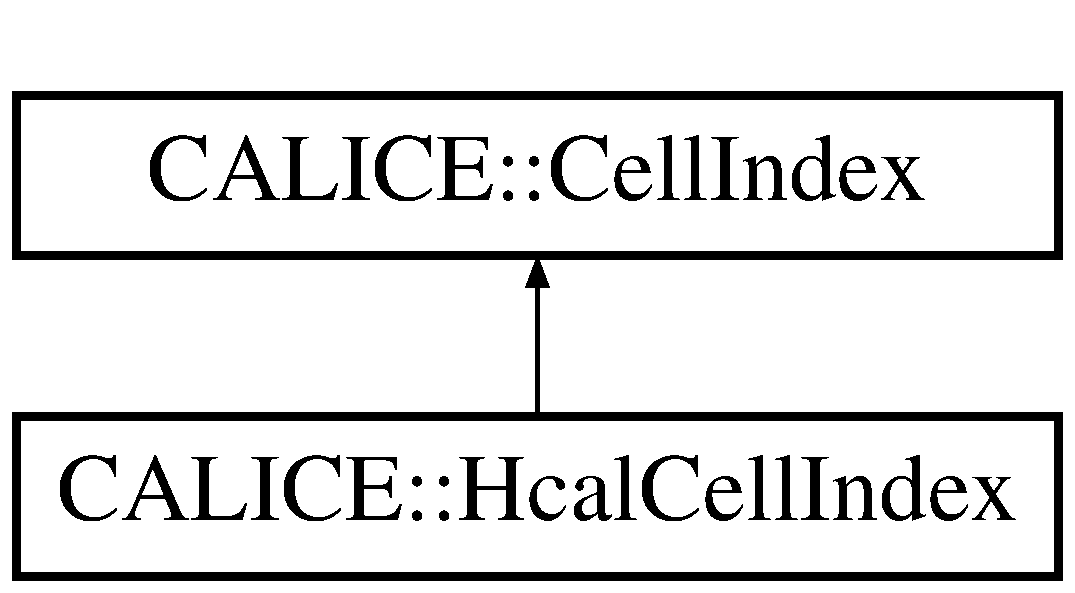
\includegraphics[height=2.000000cm]{classCALICE_1_1CellIndex}
\end{center}
\end{figure}
\subsection*{Public Member Functions}
\begin{DoxyCompactItemize}
\item 
{\bfseries Cell\-Index} (U\-Int\-\_\-t geometrical\-\_\-cell\-\_\-index)\label{classCALICE_1_1CellIndex_a4cf7ff45b88a4e2b1062ae7caaa58806}

\item 
{\bfseries Cell\-Index} (U\-Int\-\_\-t geometrical\-\_\-cell\-\_\-index, U\-Int\-\_\-t second\-\_\-cell\-\_\-index)\label{classCALICE_1_1CellIndex_aba275ac1e16f6e6e08ff9b4e4dd61f17}

\item 
{\bfseries Cell\-Index} (U\-Int\-\_\-t wafer\-\_\-row, U\-Int\-\_\-t wafer\-\_\-column, U\-Int\-\_\-t pad\-\_\-row, U\-Int\-\_\-t pad\-\_\-column, U\-Int\-\_\-t layer)\label{classCALICE_1_1CellIndex_a5ab1c3185be6a529aaf2b4476945ac94}

\item 
{\bfseries Cell\-Index} (U\-Int\-\_\-t wafer\-\_\-row, U\-Int\-\_\-t wafer\-\_\-column, U\-Int\-\_\-t pad\-\_\-row, U\-Int\-\_\-t pad\-\_\-column, U\-Int\-\_\-t layer, U\-Int\-\_\-t module\-\_\-index, U\-Int\-\_\-t module\-\_\-type, U\-Int\-\_\-t module\-\_\-\-I\-D, U\-Int\-\_\-t cell\-\_\-id, U\-Int\-\_\-t is\-Bad)\label{classCALICE_1_1CellIndex_a09201c4195f548a1ecbc740ab5178724}

\item 
{\bfseries Cell\-Index} (U\-Int\-\_\-t geometrical\-\_\-cell\-\_\-index, U\-Int\-\_\-t module\-\_\-index, U\-Int\-\_\-t module\-\_\-type, U\-Int\-\_\-t module\-\_\-\-I\-D, U\-Int\-\_\-t cell\-\_\-id, U\-Int\-\_\-t is\-Bad)\label{classCALICE_1_1CellIndex_a5c849e4daa21098f71c02773466bc2f0}

\item 
U\-Int\-\_\-t {\bf get\-Layer\-Index} () const \label{classCALICE_1_1CellIndex_a0467195bc639bda8edba4a9c96e7c0c3}

\begin{DoxyCompactList}\small\item\em Get the layer index (index labeled K in Mokka) \end{DoxyCompactList}\item 
{\bf Cell\-Index} \& {\bf set\-Layer\-Index} (U\-Int\-\_\-t layer)\label{classCALICE_1_1CellIndex_a1138c5745d65ec60aa71938eb87bc842}

\begin{DoxyCompactList}\small\item\em Set the layer index (index labeled K in Mokka) \end{DoxyCompactList}\item 
U\-Int\-\_\-t {\bf get\-Wafer\-Row} () const \label{classCALICE_1_1CellIndex_a760bda3a8354e9d93d9332220aa7c97d}

\begin{DoxyCompactList}\small\item\em Get the wafer row (index labeled M in Mokka) \end{DoxyCompactList}\item 
{\bf Cell\-Index} \& {\bf set\-Wafer\-Row} (U\-Int\-\_\-t wafer\-\_\-row)\label{classCALICE_1_1CellIndex_a4a3c7537dd7b4077e5463ae08c4c14f0}

\begin{DoxyCompactList}\small\item\em Set the wafer row (index labeled M in Mokka) \end{DoxyCompactList}\item 
U\-Int\-\_\-t {\bf get\-Wafer\-Column} () const \label{classCALICE_1_1CellIndex_a5b0755196e562f4230eb58aa820b5018}

\begin{DoxyCompactList}\small\item\em Get the wafer column (index labeled S in Mokka) \end{DoxyCompactList}\item 
{\bf Cell\-Index} \& {\bf set\-Wafer\-Column} (U\-Int\-\_\-t wafer\-\_\-column)\label{classCALICE_1_1CellIndex_a9680833ddfa0e1137ddc4e4945ecca58}

\begin{DoxyCompactList}\small\item\em Set the wafer column (index labeled S in Mokka) \end{DoxyCompactList}\item 
U\-Int\-\_\-t {\bf get\-Pad\-Row} () const \label{classCALICE_1_1CellIndex_aeecbb345a8d7a8215d020ee2ad5a73c3}

\begin{DoxyCompactList}\small\item\em Get the pad row (index labeled J in Mokka) \end{DoxyCompactList}\item 
{\bf Cell\-Index} \& {\bf set\-Pad\-Row} (U\-Int\-\_\-t pad\-\_\-row)\label{classCALICE_1_1CellIndex_a8e4528b241353e1ae52eb7febecdb371}

\begin{DoxyCompactList}\small\item\em Set the pad row (index labeled J in Mokka) \end{DoxyCompactList}\item 
U\-Int\-\_\-t {\bf get\-Pad\-Column} () const \label{classCALICE_1_1CellIndex_a37471316b7ce32ad1b19f9dc08444193}

\begin{DoxyCompactList}\small\item\em Get the pad column (index labeled I in Mokka) \end{DoxyCompactList}\item 
{\bf Cell\-Index} \& {\bf set\-Pad\-Column} (U\-Int\-\_\-t pad\-\_\-column)\label{classCALICE_1_1CellIndex_aa5e1d6c7bf39e5bfbf5ab414405b36d2}

\begin{DoxyCompactList}\small\item\em Set the pad column (index labeled I in Mokka) \end{DoxyCompactList}\item 
U\-Int\-\_\-t {\bfseries get\-Module\-Index} () const \label{classCALICE_1_1CellIndex_ad7c3aed04f51baa6a532e2dc18c0b985}

\item 
{\bf Cell\-Index} \& {\bfseries set\-Module\-Index} (U\-Int\-\_\-t module\-\_\-index)\label{classCALICE_1_1CellIndex_a87812ed0af0e2c688b21af5a7b3f53fd}

\item 
U\-Int\-\_\-t {\bfseries get\-Module\-Type} () const \label{classCALICE_1_1CellIndex_ada309da2021a56aa6bb61d0c503f2bd7}

\item 
{\bf Cell\-Index} \& {\bfseries set\-Module\-Type} (U\-Int\-\_\-t module\-\_\-type)\label{classCALICE_1_1CellIndex_aa7541e4208eb9cd7bb5401b324f539e1}

\item 
U\-Int\-\_\-t {\bfseries get\-Module\-I\-D} () const \label{classCALICE_1_1CellIndex_a77cabe65a4bd5887963f70eacef6a1b9}

\item 
{\bf Cell\-Index} \& {\bfseries set\-Module\-I\-D} (U\-Int\-\_\-t module\-\_\-\-I\-D)\label{classCALICE_1_1CellIndex_a5cfc410ec22f397a8c21c878e53ab311}

\item 
U\-Int\-\_\-t {\bfseries get\-Cell\-I\-D} () const \label{classCALICE_1_1CellIndex_a8754c16be2ec04e51661f388ff994ebf}

\item 
{\bf Cell\-Index} \& {\bfseries set\-Cell\-I\-D} (U\-Int\-\_\-t cell\-\_\-index)\label{classCALICE_1_1CellIndex_a3ecc39a5eb6b4c2d1319d113e1d8b6c3}

\item 
U\-Int\-\_\-t {\bfseries is\-Bad} () const \label{classCALICE_1_1CellIndex_a33d6d5bfcc91c6653139a73b5c6ff207}

\item 
{\bf Cell\-Index} \& {\bfseries set\-Bad} (U\-Int\-\_\-t is\-\_\-bad)\label{classCALICE_1_1CellIndex_aaedafad4a164da776eb9563f6cfecb02}

\item 
U\-Int\-\_\-t {\bf get\-Cell\-Index} () const \label{classCALICE_1_1CellIndex_a8989a0bfe43f87f5ba5d5f665cc8fd60}

\begin{DoxyCompactList}\small\item\em Get the Mokka conform cell index. \end{DoxyCompactList}\item 
{\bf Cell\-Index} \& {\bf set\-Cell\-Index} (U\-Int\-\_\-t mokka\-\_\-cell\-\_\-index)\label{classCALICE_1_1CellIndex_a06927c6c271b586b2d4f2349ad0a0058}

\begin{DoxyCompactList}\small\item\em Set the Mokka conform cell index. \end{DoxyCompactList}\item 
U\-Int\-\_\-t {\bf get\-Second\-Index} () const \label{classCALICE_1_1CellIndex_a62457057612992847f0d1a6791e5eed0}

\begin{DoxyCompactList}\small\item\em Get the 2nd cell index. \end{DoxyCompactList}\item 
{\bf Cell\-Index} \& {\bf set\-Second\-Index} (U\-Int\-\_\-t cell\-I\-D1)\label{classCALICE_1_1CellIndex_acee8e762e051e2e12e0bfab43be8c441}

\begin{DoxyCompactList}\small\item\em Set the 2nd cell index. \end{DoxyCompactList}\end{DoxyCompactItemize}
\subsection*{Private Attributes}
\begin{DoxyCompactItemize}
\item 
U\-Int\-\_\-t {\bfseries \-\_\-index}\label{classCALICE_1_1CellIndex_a0422c3652b611890e2c610eef01fc43e}

\item 
U\-Int\-\_\-t {\bfseries \-\_\-second}\label{classCALICE_1_1CellIndex_adcca7440632d6d8b81aa514a89035b6f}

\end{DoxyCompactItemize}


\subsection{Detailed Description}
The Mokka conform cell index. 

The cell index encodes the wafer column, and row, pad column and row, and the layer into one index. The wafer 0,0 is in the lower right corner (following a right handed coordinate frame ) looking in beam direction at the detector fron plate. Similar the pad 0,0 of each wafer is located in the lower right corner of the wafer. Encoding for the E\-C\-A\-L\-: \begin{TabularC}{2}
\hline
M\-:3,&wafer row \\\cline{1-2}
S-\/1\-:3,&wafer column \\\cline{1-2}
I\-:9,&pad coloumn \\\cline{1-2}
J\-:9,&pad row \\\cline{1-2}
K\-:6&layer \\\cline{1-2}
\end{TabularC}


Definition at line 102 of file Cell\-Index.\-hh.



The documentation for this class was generated from the following file\-:\begin{DoxyCompactItemize}
\item 
Cell\-Index.\-hh\end{DoxyCompactItemize}

\section{C\-A\-L\-I\-C\-E\-:\-:Cell\-Iterator Class Reference}
\label{classCALICE_1_1CellIterator}\index{C\-A\-L\-I\-C\-E\-::\-Cell\-Iterator@{C\-A\-L\-I\-C\-E\-::\-Cell\-Iterator}}


iterator to run over all valid (Mokka) cell I\-Ds  




{\ttfamily \#include $<$Cell\-Iterator.\-hh$>$}

\subsection*{Public Member Functions}
\begin{DoxyCompactItemize}
\item 
{\bfseries Cell\-Iterator} (const {\bf Mapper} $\ast$mapper, const unsigned int index=0)\label{classCALICE_1_1CellIterator_a55f049561c6efd49d8ac05d8fd1892d9}

\item 
void {\bf operator++} ()\label{classCALICE_1_1CellIterator_aa8632dfb854dab0d3afa78eee2d3e4fe}

\begin{DoxyCompactList}\small\item\em jump to the next valid (Mokka) cell I\-D \end{DoxyCompactList}\item 
bool {\bf operator!=} (const {\bf Cell\-Iterator} \&other) const \label{classCALICE_1_1CellIterator_afad05336400eeb213d96a7bb837e47da}

\begin{DoxyCompactList}\small\item\em compare if two iterators are not equal \end{DoxyCompactList}\item 
bool {\bf operator==} (const {\bf Cell\-Iterator} \&other) const \label{classCALICE_1_1CellIterator_a16d97b72ac170520e4ddbcb54ae2b7ae}

\begin{DoxyCompactList}\small\item\em compare if two iterators are equal \end{DoxyCompactList}\item 
int {\bf operator$\ast$} () const 
\begin{DoxyCompactList}\small\item\em access to the current (Mokka) cell I\-D \end{DoxyCompactList}\end{DoxyCompactItemize}
\subsection*{Protected Attributes}
\begin{DoxyCompactItemize}
\item 
const {\bf Mapper} $\ast$ {\bfseries \-\_\-mapper}\label{classCALICE_1_1CellIterator_ac61b53457ed96438d6a3c20658a8b470}

\item 
unsigned int {\bfseries \-\_\-index}\label{classCALICE_1_1CellIterator_a3ec4eb2ac9ee642f134773d08b382281}

\item 
int {\bfseries \-\_\-current\-Cell\-I\-D}\label{classCALICE_1_1CellIterator_ae8e06dc84e48a482fd2f6ee28d5833eb}

\end{DoxyCompactItemize}


\subsection{Detailed Description}
iterator to run over all valid (Mokka) cell I\-Ds 

To access the Cell\-I\-D use the $\ast$() operator.

\begin{DoxyAuthor}{Author}
{\tt Benjamin.\-Lutz@desy.\-de} 
\end{DoxyAuthor}
\begin{DoxyDate}{Date}
June 2009 
\end{DoxyDate}


Definition at line 18 of file Cell\-Iterator.\-hh.



\subsection{Member Function Documentation}
\index{C\-A\-L\-I\-C\-E\-::\-Cell\-Iterator@{C\-A\-L\-I\-C\-E\-::\-Cell\-Iterator}!operator$\ast$@{operator$\ast$}}
\index{operator$\ast$@{operator$\ast$}!CALICE::CellIterator@{C\-A\-L\-I\-C\-E\-::\-Cell\-Iterator}}
\subsubsection[{operator$\ast$}]{\setlength{\rightskip}{0pt plus 5cm}int C\-A\-L\-I\-C\-E\-::\-Cell\-Iterator\-::operator$\ast$ (
\begin{DoxyParamCaption}
{}
\end{DoxyParamCaption}
) const\hspace{0.3cm}{\ttfamily [inline]}}\label{classCALICE_1_1CellIterator_ad5a74f9ea744a9ccac7f40a549ddd4cf}


access to the current (Mokka) cell I\-D 

\begin{DoxyReturn}{Returns}
the current cell I\-D 
\end{DoxyReturn}


Definition at line 43 of file Cell\-Iterator.\-hh.



The documentation for this class was generated from the following files\-:\begin{DoxyCompactItemize}
\item 
Cell\-Iterator.\-hh\item 
Cell\-Iterator.\-cc\end{DoxyCompactItemize}

\section{C\-A\-L\-I\-C\-E\-:\-:Cell\-Mapping\-Hcal Class Reference}
\label{classCALICE_1_1CellMappingHcal}\index{C\-A\-L\-I\-C\-E\-::\-Cell\-Mapping\-Hcal@{C\-A\-L\-I\-C\-E\-::\-Cell\-Mapping\-Hcal}}


Example for a simple mapping class based on the L\-C\-Fixed\-Object template.  




{\ttfamily \#include $<$Cell\-Mapping\-Hcal.\-hh$>$}

Inheritance diagram for C\-A\-L\-I\-C\-E\-:\-:Cell\-Mapping\-Hcal\-:\begin{figure}[H]
\begin{center}
\leavevmode
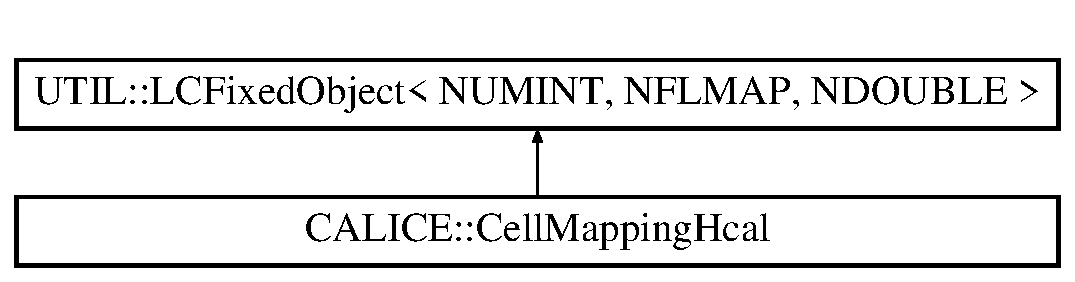
\includegraphics[height=2.000000cm]{classCALICE_1_1CellMappingHcal}
\end{center}
\end{figure}
\subsection*{Public Member Functions}
\begin{DoxyCompactItemize}
\item 
{\bf Cell\-Mapping\-Hcal} (int icrate, int islot, int ife, int imul, int iadc, int icoord, int jcoord, int kcoord)\label{classCALICE_1_1CellMappingHcal_a180c0b169a7f2c69770ae551aa4c776d}

\begin{DoxyCompactList}\small\item\em Convenient c'tor. \end{DoxyCompactList}\item 
{\bf Cell\-Mapping\-Hcal} (L\-C\-Object $\ast$obj)\label{classCALICE_1_1CellMappingHcal_a0da96ba25246cd5cca90973d362e6c87}

\begin{DoxyCompactList}\small\item\em 'Copy constructor' needed to interpret L\-C\-Collection read from file/database. \end{DoxyCompactList}\item 
virtual {\bf $\sim$\-Cell\-Mapping\-Hcal} ()\label{classCALICE_1_1CellMappingHcal_a83d82878315eb6feafff6da924cb0b3e}

\begin{DoxyCompactList}\small\item\em Important for memory handling. \end{DoxyCompactList}\item 
int {\bf get\-Elec\-Channel} ()\label{classCALICE_1_1CellMappingHcal_ac7b97417224ddeba13c73d7659484ed0}

\begin{DoxyCompactList}\small\item\em the class interface\-: \end{DoxyCompactList}\item 
int {\bfseries get\-Cell\-I\-D} ()\label{classCALICE_1_1CellMappingHcal_a5e62c1a1fa22a5d93b59734f5c307fbf}

\item 
short {\bf get\-Cell\-Index} (std\-::string)\label{classCALICE_1_1CellMappingHcal_a4beaa39635a9c718ecbcb98ee336bf4e}

\begin{DoxyCompactList}\small\item\em convenient getter functions \end{DoxyCompactList}\item 
short {\bfseries get\-Crate\-I\-D} ()\label{classCALICE_1_1CellMappingHcal_a5828458b37828b0bf81007b081bdefdc}

\item 
short {\bfseries get\-Slot\-I\-D} ()\label{classCALICE_1_1CellMappingHcal_a83ae95e889acadd9e666421021fc94bd}

\item 
short {\bfseries get\-Fe\-I\-D} ()\label{classCALICE_1_1CellMappingHcal_a0a0f4e3978887fcb96c2990ad98c7ff8}

\item 
short {\bfseries get\-Mul\-I\-D} ()\label{classCALICE_1_1CellMappingHcal_ac15468dcd4948f44a67978680748aa54}

\item 
short {\bfseries get\-Adc\-I\-D} ()\label{classCALICE_1_1CellMappingHcal_a877867886306a01fe319eab0b00f7256}

\item 
void {\bf print} (std\-::ostream \&os)\label{classCALICE_1_1CellMappingHcal_a2ffe99f7db6ac95b8e972b37d189f6da}

\begin{DoxyCompactList}\small\item\em Convenient print method. \end{DoxyCompactList}\item 
const std\-::string {\bf get\-Type\-Name} () const \label{classCALICE_1_1CellMappingHcal_a03e821c39e5e6452c89954ddcc5038c8}

\begin{DoxyCompactList}\small\item\em Type definition. \end{DoxyCompactList}\item 
const std\-::string {\bf get\-Data\-Description} () const 
\begin{DoxyCompactList}\small\item\em Data description, needed e.\-g. \end{DoxyCompactList}\end{DoxyCompactItemize}
\subsection*{Private Attributes}
\begin{DoxyCompactItemize}
\item 
short {\bf \-\_\-index}\label{classCALICE_1_1CellMappingHcal_ac042db1cac41c0a080364c6ed8e6e4f5}

\begin{DoxyCompactList}\small\item\em i,j or k Index of the cell id \end{DoxyCompactList}\end{DoxyCompactItemize}


\subsection{Detailed Description}
Example for a simple mapping class based on the L\-C\-Fixed\-Object template. 

L\-C\-Fixed\-Object uses an instance of L\-C\-Generic\-Object\-Impl that holds the data, thus there is no overhead when the data is read from a database or file for copying it to some local structure (Decorator pattern).\par
 

Definition at line 40 of file Cell\-Mapping\-Hcal.\-hh.



\subsection{Member Function Documentation}
\index{C\-A\-L\-I\-C\-E\-::\-Cell\-Mapping\-Hcal@{C\-A\-L\-I\-C\-E\-::\-Cell\-Mapping\-Hcal}!get\-Data\-Description@{get\-Data\-Description}}
\index{get\-Data\-Description@{get\-Data\-Description}!CALICE::CellMappingHcal@{C\-A\-L\-I\-C\-E\-::\-Cell\-Mapping\-Hcal}}
\subsubsection[{get\-Data\-Description}]{\setlength{\rightskip}{0pt plus 5cm}const std\-::string C\-A\-L\-I\-C\-E\-::\-Cell\-Mapping\-Hcal\-::get\-Data\-Description (
\begin{DoxyParamCaption}
{}
\end{DoxyParamCaption}
) const\hspace{0.3cm}{\ttfamily [inline]}}\label{classCALICE_1_1CellMappingHcal_a703c49c4ee36f2faf9ff744afc9bf098}


Data description, needed e.\-g. 

by graphical interface to L\-C\-C\-D 

Definition at line 96 of file Cell\-Mapping\-Hcal.\-hh.



The documentation for this class was generated from the following files\-:\begin{DoxyCompactItemize}
\item 
Cell\-Mapping\-Hcal.\-hh\item 
Cell\-Mapping\-Hcal.\-cc\end{DoxyCompactItemize}

\section{C\-A\-L\-I\-C\-E\-:\-:Cell\-Neighbour\-Calculator Class Reference}
\label{classCALICE_1_1CellNeighbourCalculator}\index{C\-A\-L\-I\-C\-E\-::\-Cell\-Neighbour\-Calculator@{C\-A\-L\-I\-C\-E\-::\-Cell\-Neighbour\-Calculator}}


class to calculate all neighbour cells  




{\ttfamily \#include $<$Cell\-Neighbour\-Calculator.\-hh$>$}

\subsection*{Public Member Functions}
\begin{DoxyCompactItemize}
\item 
{\bf Cell\-Neighbour\-Calculator} (const {\bf Mapper} $\ast$mapper)
\begin{DoxyCompactList}\small\item\em constructor \end{DoxyCompactList}\item 
lcio\-::\-L\-C\-Collection $\ast$ {\bf get\-Neighbours} () const 
\begin{DoxyCompactList}\small\item\em get cell neighbours for all valid cells \end{DoxyCompactList}\item 
void {\bf get\-Neighbours} ({\bf Mapped\-Container}$<$ {\bf Cell\-Neighbours} $>$ $\ast$container) const 
\begin{DoxyCompactList}\small\item\em get cell neighbours for all valid cells \end{DoxyCompactList}\end{DoxyCompactItemize}
\subsection*{Protected Member Functions}
\begin{DoxyCompactItemize}
\item 
void {\bfseries check\-For\-Cell} (const unsigned int i, const unsigned int j, const unsigned int k, std\-::set$<$ int $>$ \&cell\-I\-Dset) const \label{classCALICE_1_1CellNeighbourCalculator_af07fc90a40e8baaf67fac09d53ee2988}

\item 
{\bf Cell\-Neighbours} $\ast$ {\bfseries get\-Neighbours} (const int cell\-I\-D) const \label{classCALICE_1_1CellNeighbourCalculator_a687feccba274d8aa4ab40b2c37bf4261}

\end{DoxyCompactItemize}
\subsection*{Private Attributes}
\begin{DoxyCompactItemize}
\item 
const {\bf Mapper} $\ast$ {\bfseries \-\_\-mapper}\label{classCALICE_1_1CellNeighbourCalculator_a73c7934a2879e61cf0946e5539067181}

\end{DoxyCompactItemize}


\subsection{Detailed Description}
class to calculate all neighbour cells 

\begin{DoxyAuthor}{Author}
{\tt Benjamin.\-Lutz@desy.\-de} 
\end{DoxyAuthor}
\begin{DoxyVersion}{Version}
0.\-1 
\end{DoxyVersion}
\begin{DoxyDate}{Date}
June 2009 
\end{DoxyDate}


Definition at line 22 of file Cell\-Neighbour\-Calculator.\-hh.



\subsection{Constructor \& Destructor Documentation}
\index{C\-A\-L\-I\-C\-E\-::\-Cell\-Neighbour\-Calculator@{C\-A\-L\-I\-C\-E\-::\-Cell\-Neighbour\-Calculator}!Cell\-Neighbour\-Calculator@{Cell\-Neighbour\-Calculator}}
\index{Cell\-Neighbour\-Calculator@{Cell\-Neighbour\-Calculator}!CALICE::CellNeighbourCalculator@{C\-A\-L\-I\-C\-E\-::\-Cell\-Neighbour\-Calculator}}
\subsubsection[{Cell\-Neighbour\-Calculator}]{\setlength{\rightskip}{0pt plus 5cm}C\-A\-L\-I\-C\-E\-::\-Cell\-Neighbour\-Calculator\-::\-Cell\-Neighbour\-Calculator (
\begin{DoxyParamCaption}
\item[{const {\bf Mapper} $\ast$}]{mapper}
\end{DoxyParamCaption}
)}\label{classCALICE_1_1CellNeighbourCalculator_abd2c59c1797a382c0518df7efd9a3108}


constructor 


\begin{DoxyParams}{Parameters}
{\em mapper} & \doxyref{Mapper}{p.}{classCALICE_1_1Mapper} that holds the mapping information from which the neighbours can be generated. \\
\hline
\end{DoxyParams}


Definition at line 10 of file Cell\-Neighbour\-Calculator.\-cc.



\subsection{Member Function Documentation}
\index{C\-A\-L\-I\-C\-E\-::\-Cell\-Neighbour\-Calculator@{C\-A\-L\-I\-C\-E\-::\-Cell\-Neighbour\-Calculator}!get\-Neighbours@{get\-Neighbours}}
\index{get\-Neighbours@{get\-Neighbours}!CALICE::CellNeighbourCalculator@{C\-A\-L\-I\-C\-E\-::\-Cell\-Neighbour\-Calculator}}
\subsubsection[{get\-Neighbours}]{\setlength{\rightskip}{0pt plus 5cm}lcio\-::\-L\-C\-Collection $\ast$ C\-A\-L\-I\-C\-E\-::\-Cell\-Neighbour\-Calculator\-::get\-Neighbours (
\begin{DoxyParamCaption}
{}
\end{DoxyParamCaption}
) const}\label{classCALICE_1_1CellNeighbourCalculator_a029af1aa53034010a443d205c554e92b}


get cell neighbours for all valid cells 

\begin{DoxyReturn}{Returns}
L\-C\-Collection of \doxyref{Cell\-Neighbours}{p.}{classCALICE_1_1CellNeighbours} objects 
\end{DoxyReturn}


Definition at line 88 of file Cell\-Neighbour\-Calculator.\-cc.



References C\-A\-L\-I\-C\-E\-::\-Mapper\-::begin(), and C\-A\-L\-I\-C\-E\-::\-Mapper\-::end().



Referenced by get\-Neighbours().

\index{C\-A\-L\-I\-C\-E\-::\-Cell\-Neighbour\-Calculator@{C\-A\-L\-I\-C\-E\-::\-Cell\-Neighbour\-Calculator}!get\-Neighbours@{get\-Neighbours}}
\index{get\-Neighbours@{get\-Neighbours}!CALICE::CellNeighbourCalculator@{C\-A\-L\-I\-C\-E\-::\-Cell\-Neighbour\-Calculator}}
\subsubsection[{get\-Neighbours}]{\setlength{\rightskip}{0pt plus 5cm}void C\-A\-L\-I\-C\-E\-::\-Cell\-Neighbour\-Calculator\-::get\-Neighbours (
\begin{DoxyParamCaption}
\item[{{\bf Mapped\-Container}$<$ {\bf Cell\-Neighbours} $>$ $\ast$}]{container}
\end{DoxyParamCaption}
) const}\label{classCALICE_1_1CellNeighbourCalculator_ad17cd5438d923800b419794ffa853386}


get cell neighbours for all valid cells 


\begin{DoxyParams}[1]{Parameters}
\mbox{\tt out}  & {\em container} & \doxyref{Mapped\-Container}{p.}{classCALICE_1_1MappedContainer} where the \doxyref{Cell\-Neighbours}{p.}{classCALICE_1_1CellNeighbours} objects should be stored \\
\hline
\end{DoxyParams}


Definition at line 103 of file Cell\-Neighbour\-Calculator.\-cc.



References C\-A\-L\-I\-C\-E\-::\-Mapper\-::begin(), C\-A\-L\-I\-C\-E\-::\-Mapped\-Container$<$ T $>$\-::clear(), C\-A\-L\-I\-C\-E\-::\-Mapper\-::end(), C\-A\-L\-I\-C\-E\-::\-Mapped\-Container$<$ T $>$\-::fill\-By\-Cell\-I\-D(), and get\-Neighbours().



The documentation for this class was generated from the following files\-:\begin{DoxyCompactItemize}
\item 
Cell\-Neighbour\-Calculator.\-hh\item 
Cell\-Neighbour\-Calculator.\-cc\end{DoxyCompactItemize}

\section{C\-A\-L\-I\-C\-E\-:\-:Cell\-Neighbours Class Reference}
\label{classCALICE_1_1CellNeighbours}\index{C\-A\-L\-I\-C\-E\-::\-Cell\-Neighbours@{C\-A\-L\-I\-C\-E\-::\-Cell\-Neighbours}}


class to hold information of neighbouring cells  




{\ttfamily \#include $<$Cell\-Neighbours.\-hh$>$}

Inheritance diagram for C\-A\-L\-I\-C\-E\-:\-:Cell\-Neighbours\-:\begin{figure}[H]
\begin{center}
\leavevmode
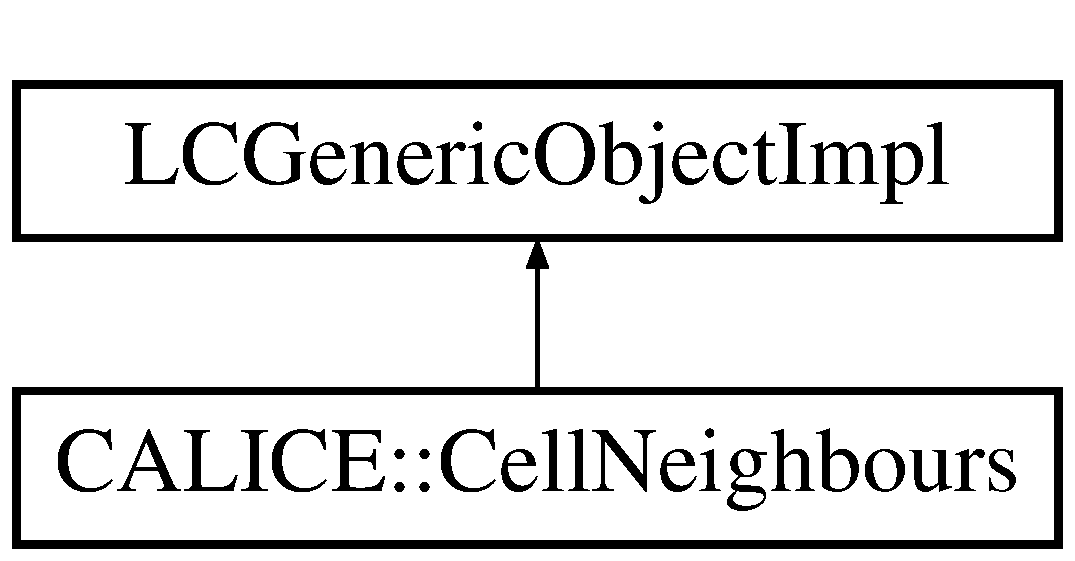
\includegraphics[height=2.000000cm]{classCALICE_1_1CellNeighbours}
\end{center}
\end{figure}
\subsection*{Public Types}
\begin{DoxyCompactItemize}
\item 
enum {\bf E\-Neighbour\-Type} \{ {\bf direct}, 
{\bf corner}, 
{\bfseries k\-\_\-\-Nneighbour\-Types}
 \}
\begin{DoxyCompactList}\small\item\em neighbour type \end{DoxyCompactList}\item 
enum {\bf E\-Neighbour\-Location} \{ {\bf module}, 
{\bf forward}, 
{\bf backward}, 
{\bfseries k\-\_\-\-Nneighbour\-Locations}
 \}
\begin{DoxyCompactList}\small\item\em neighbour location \end{DoxyCompactList}\end{DoxyCompactItemize}
\subsection*{Public Member Functions}
\begin{DoxyCompactItemize}
\item 
{\bf Cell\-Neighbours} (const lcio\-::\-L\-C\-Object $\ast$obj)
\begin{DoxyCompactList}\small\item\em copy constructor \end{DoxyCompactList}\item 
{\bf Cell\-Neighbours} (const lcio\-::\-L\-C\-Generic\-Object \&obj)
\begin{DoxyCompactList}\small\item\em copy constructor \end{DoxyCompactList}\item 
{\bf Cell\-Neighbours} (const int cell\-I\-D)
\begin{DoxyCompactList}\small\item\em constructor \end{DoxyCompactList}\item 
void {\bf add\-Neighbour} (const int cell\-I\-D, const {\bf E\-Neighbour\-Type} type, const {\bf E\-Neighbour\-Location} location)
\begin{DoxyCompactList}\small\item\em add a neighbour cell \end{DoxyCompactList}\item 
int {\bf get\-Cell\-I\-D} () const 
\begin{DoxyCompactList}\small\item\em get (Mokka) cell I\-D of master cell \end{DoxyCompactList}\item 
const std\-::vector$<$ int $>$ \& {\bf get\-Neighbours} (const {\bf E\-Neighbour\-Type} type, const {\bf E\-Neighbour\-Location} location) const 
\begin{DoxyCompactList}\small\item\em get vector of cell neighbours \end{DoxyCompactList}\item 
const std\-::vector$<$ int $>$ {\bf get\-Neighbours} (const {\bf E\-Neighbour\-Type} type) const 
\begin{DoxyCompactList}\small\item\em get vector of cell neighbours \end{DoxyCompactList}\item 
const std\-::vector$<$ int $>$ {\bf get\-Neighbours} (const {\bf E\-Neighbour\-Location} location) const 
\begin{DoxyCompactList}\small\item\em get vector of cell neighbours \end{DoxyCompactList}\item 
const std\-::vector$<$ int $>$ {\bf get\-Neighbours} () const 
\begin{DoxyCompactList}\small\item\em get vector of cell neighbours \end{DoxyCompactList}\item 
const std\-::string {\bf get\-Type\-Name} () const 
\item 
const std\-::string {\bf get\-Data\-Description} () const 
\end{DoxyCompactItemize}
\subsection*{Private Types}
\begin{DoxyCompactItemize}
\item 
enum {\bfseries E\-Int} \{ {\bfseries k\-\_\-\-Cell\-I\-D}, 
{\bfseries k\-\_\-\-Nfixed\-Numbers}
 \}
\end{DoxyCompactItemize}
\subsection*{Private Member Functions}
\begin{DoxyCompactItemize}
\item 
void {\bfseries copy\-From\-L\-C\-Generic\-Object} (const lcio\-::\-L\-C\-Generic\-Object \&obj)\label{classCALICE_1_1CellNeighbours_a399c77122e29b11f0579209c2879a27c}

\item 
void {\bfseries load\-Values} ()\label{classCALICE_1_1CellNeighbours_a201d35e317d7483f2ae8807c5dd09ae6}

\item 
void {\bfseries save\-Values} ()\label{classCALICE_1_1CellNeighbours_a65f20f02b3553a3a0abb5cf9483f3aee}

\end{DoxyCompactItemize}
\subsection*{Private Attributes}
\begin{DoxyCompactItemize}
\item 
std\-::ostringstream {\bfseries \-\_\-data\-Description}\label{classCALICE_1_1CellNeighbours_aaf784e8920b14763e7daedf2b88499dc}

\item 
std\-::vector$<$ int $>$ {\bfseries \-\_\-neighbour\-Vectors} [k\-\_\-\-Nneighbour\-Types][k\-\_\-\-Nneighbour\-Locations]\label{classCALICE_1_1CellNeighbours_a0f613c9c20d750a3399978eb21263328}

\end{DoxyCompactItemize}
\subsection*{Static Private Attributes}
\begin{DoxyCompactItemize}
\item 
static const std\-::string {\bfseries neighbour\-Fixed\-Names} [k\-\_\-\-Nfixed\-Numbers] = \{ \char`\"{}cell\-I\-D\char`\"{} \}\label{classCALICE_1_1CellNeighbours_aee105726874440a5f4c3bfbae89de46b}

\item 
static const std\-::string {\bfseries neighbour\-Type\-Names} [k\-\_\-\-Nneighbour\-Types]
\item 
static const std\-::string {\bfseries neighbour\-Location\-Names} [k\-\_\-\-Nneighbour\-Locations]
\end{DoxyCompactItemize}


\subsection{Detailed Description}
class to hold information of neighbouring cells 

\begin{DoxyAuthor}{Author}
{\tt Benjamin.\-Lutz@desy.\-de} 
\end{DoxyAuthor}
\begin{DoxyVersion}{Version}
0.\-1 
\end{DoxyVersion}
\begin{DoxyDate}{Date}
June 2009 
\end{DoxyDate}


Definition at line 21 of file Cell\-Neighbours.\-hh.



\subsection{Member Enumeration Documentation}
\index{C\-A\-L\-I\-C\-E\-::\-Cell\-Neighbours@{C\-A\-L\-I\-C\-E\-::\-Cell\-Neighbours}!E\-Neighbour\-Location@{E\-Neighbour\-Location}}
\index{E\-Neighbour\-Location@{E\-Neighbour\-Location}!CALICE::CellNeighbours@{C\-A\-L\-I\-C\-E\-::\-Cell\-Neighbours}}
\subsubsection[{E\-Neighbour\-Location}]{\setlength{\rightskip}{0pt plus 5cm}enum {\bf C\-A\-L\-I\-C\-E\-::\-Cell\-Neighbours\-::\-E\-Neighbour\-Location}}\label{classCALICE_1_1CellNeighbours_affedb8e9d258cd5d11a65c921b92977f}


neighbour location 

\begin{Desc}
\item[Enumerator]\par
\begin{description}
\index{module@{module}!C\-A\-L\-I\-C\-E\-::\-Cell\-Neighbours@{C\-A\-L\-I\-C\-E\-::\-Cell\-Neighbours}}\index{C\-A\-L\-I\-C\-E\-::\-Cell\-Neighbours@{C\-A\-L\-I\-C\-E\-::\-Cell\-Neighbours}!module@{module}}\item[{\em 
module\label{classCALICE_1_1CellNeighbours_affedb8e9d258cd5d11a65c921b92977fabb1923c9ce736bd00b553168bce257b1}
}]neighbours within the same module \index{forward@{forward}!C\-A\-L\-I\-C\-E\-::\-Cell\-Neighbours@{C\-A\-L\-I\-C\-E\-::\-Cell\-Neighbours}}\index{C\-A\-L\-I\-C\-E\-::\-Cell\-Neighbours@{C\-A\-L\-I\-C\-E\-::\-Cell\-Neighbours}!forward@{forward}}\item[{\em 
forward\label{classCALICE_1_1CellNeighbours_affedb8e9d258cd5d11a65c921b92977fa4e5216e19431a86e213595e2c942a68d}
}]neighbours in the next module (beam direction) \index{backward@{backward}!C\-A\-L\-I\-C\-E\-::\-Cell\-Neighbours@{C\-A\-L\-I\-C\-E\-::\-Cell\-Neighbours}}\index{C\-A\-L\-I\-C\-E\-::\-Cell\-Neighbours@{C\-A\-L\-I\-C\-E\-::\-Cell\-Neighbours}!backward@{backward}}\item[{\em 
backward\label{classCALICE_1_1CellNeighbours_affedb8e9d258cd5d11a65c921b92977fa79354e5a35520f80687b76faf7aa62a4}
}]neighbours in the previous module \end{description}
\end{Desc}


Definition at line 44 of file Cell\-Neighbours.\-hh.

\index{C\-A\-L\-I\-C\-E\-::\-Cell\-Neighbours@{C\-A\-L\-I\-C\-E\-::\-Cell\-Neighbours}!E\-Neighbour\-Type@{E\-Neighbour\-Type}}
\index{E\-Neighbour\-Type@{E\-Neighbour\-Type}!CALICE::CellNeighbours@{C\-A\-L\-I\-C\-E\-::\-Cell\-Neighbours}}
\subsubsection[{E\-Neighbour\-Type}]{\setlength{\rightskip}{0pt plus 5cm}enum {\bf C\-A\-L\-I\-C\-E\-::\-Cell\-Neighbours\-::\-E\-Neighbour\-Type}}\label{classCALICE_1_1CellNeighbours_a89a97dd297d98694875175c22f6c80b9}


neighbour type 

\begin{Desc}
\item[Enumerator]\par
\begin{description}
\index{direct@{direct}!C\-A\-L\-I\-C\-E\-::\-Cell\-Neighbours@{C\-A\-L\-I\-C\-E\-::\-Cell\-Neighbours}}\index{C\-A\-L\-I\-C\-E\-::\-Cell\-Neighbours@{C\-A\-L\-I\-C\-E\-::\-Cell\-Neighbours}!direct@{direct}}\item[{\em 
direct\label{classCALICE_1_1CellNeighbours_a89a97dd297d98694875175c22f6c80b9ae61ea93bbf272464e5403ddfbf0a60fc}
}]describes the neighbours that have a common side/surface with the original cell \index{corner@{corner}!C\-A\-L\-I\-C\-E\-::\-Cell\-Neighbours@{C\-A\-L\-I\-C\-E\-::\-Cell\-Neighbours}}\index{C\-A\-L\-I\-C\-E\-::\-Cell\-Neighbours@{C\-A\-L\-I\-C\-E\-::\-Cell\-Neighbours}!corner@{corner}}\item[{\em 
corner\label{classCALICE_1_1CellNeighbours_a89a97dd297d98694875175c22f6c80b9a2f63e34121a3a79e0232d0568e51c154}
}]E\-Neighbour\-Type\-::corner describes the neighbours that connect to the original cell via a corner \end{description}
\end{Desc}


Definition at line 34 of file Cell\-Neighbours.\-hh.



\subsection{Constructor \& Destructor Documentation}
\index{C\-A\-L\-I\-C\-E\-::\-Cell\-Neighbours@{C\-A\-L\-I\-C\-E\-::\-Cell\-Neighbours}!Cell\-Neighbours@{Cell\-Neighbours}}
\index{Cell\-Neighbours@{Cell\-Neighbours}!CALICE::CellNeighbours@{C\-A\-L\-I\-C\-E\-::\-Cell\-Neighbours}}
\subsubsection[{Cell\-Neighbours}]{\setlength{\rightskip}{0pt plus 5cm}C\-A\-L\-I\-C\-E\-::\-Cell\-Neighbours\-::\-Cell\-Neighbours (
\begin{DoxyParamCaption}
\item[{const lcio\-::\-L\-C\-Object $\ast$}]{obj}
\end{DoxyParamCaption}
)}\label{classCALICE_1_1CellNeighbours_a190a549359a8902d0d8c5386b23861cd}


copy constructor 

This constructor is meant to copy-\/convert a \doxyref{Cell\-Neighbours}{p.}{classCALICE_1_1CellNeighbours} object from a L\-C\-Collection\-::get\-Element\-At() call. In contrary to other L\-C\-Generic\-Object derivates, this doesn't reference to the old object, but makes a full copy.


\begin{DoxyParams}[1]{Parameters}
\mbox{\tt in}  & {\em obj} & L\-C\-Object pointer to a \doxyref{Cell\-Neighbours}{p.}{classCALICE_1_1CellNeighbours} object \\
\hline
\end{DoxyParams}


Definition at line 15 of file Cell\-Neighbours.\-cc.

\index{C\-A\-L\-I\-C\-E\-::\-Cell\-Neighbours@{C\-A\-L\-I\-C\-E\-::\-Cell\-Neighbours}!Cell\-Neighbours@{Cell\-Neighbours}}
\index{Cell\-Neighbours@{Cell\-Neighbours}!CALICE::CellNeighbours@{C\-A\-L\-I\-C\-E\-::\-Cell\-Neighbours}}
\subsubsection[{Cell\-Neighbours}]{\setlength{\rightskip}{0pt plus 5cm}C\-A\-L\-I\-C\-E\-::\-Cell\-Neighbours\-::\-Cell\-Neighbours (
\begin{DoxyParamCaption}
\item[{const lcio\-::\-L\-C\-Generic\-Object \&}]{obj}
\end{DoxyParamCaption}
)}\label{classCALICE_1_1CellNeighbours_a34ce6eed0846685f8b32342f5249820f}


copy constructor 

This constructor is meant to copy-\/convert a \doxyref{Cell\-Neighbours}{p.}{classCALICE_1_1CellNeighbours} object from a L\-C\-Generic\-Object.


\begin{DoxyParams}[1]{Parameters}
\mbox{\tt in}  & {\em obj} & L\-C\-Generic\-Object of type \doxyref{Cell\-Neighbours}{p.}{classCALICE_1_1CellNeighbours} which should be copied \\
\hline
\end{DoxyParams}


Definition at line 25 of file Cell\-Neighbours.\-cc.

\index{C\-A\-L\-I\-C\-E\-::\-Cell\-Neighbours@{C\-A\-L\-I\-C\-E\-::\-Cell\-Neighbours}!Cell\-Neighbours@{Cell\-Neighbours}}
\index{Cell\-Neighbours@{Cell\-Neighbours}!CALICE::CellNeighbours@{C\-A\-L\-I\-C\-E\-::\-Cell\-Neighbours}}
\subsubsection[{Cell\-Neighbours}]{\setlength{\rightskip}{0pt plus 5cm}C\-A\-L\-I\-C\-E\-::\-Cell\-Neighbours\-::\-Cell\-Neighbours (
\begin{DoxyParamCaption}
\item[{const int}]{cell\-I\-D}
\end{DoxyParamCaption}
)}\label{classCALICE_1_1CellNeighbours_ad6d1861dd68ea60d4b3020fd8b623c49}


constructor 


\begin{DoxyParams}[1]{Parameters}
\mbox{\tt in}  & {\em cell\-I\-D} & (Mokka) cell I\-D of the master cell \\
\hline
\end{DoxyParams}


Definition at line 44 of file Cell\-Neighbours.\-cc.



\subsection{Member Function Documentation}
\index{C\-A\-L\-I\-C\-E\-::\-Cell\-Neighbours@{C\-A\-L\-I\-C\-E\-::\-Cell\-Neighbours}!add\-Neighbour@{add\-Neighbour}}
\index{add\-Neighbour@{add\-Neighbour}!CALICE::CellNeighbours@{C\-A\-L\-I\-C\-E\-::\-Cell\-Neighbours}}
\subsubsection[{add\-Neighbour}]{\setlength{\rightskip}{0pt plus 5cm}void C\-A\-L\-I\-C\-E\-::\-Cell\-Neighbours\-::add\-Neighbour (
\begin{DoxyParamCaption}
\item[{const int}]{cell\-I\-D, }
\item[{const {\bf E\-Neighbour\-Type}}]{type, }
\item[{const {\bf E\-Neighbour\-Location}}]{location}
\end{DoxyParamCaption}
)}\label{classCALICE_1_1CellNeighbours_ab67f7a002e853e749d4f376f423728e6}


add a neighbour cell 


\begin{DoxyParams}[1]{Parameters}
\mbox{\tt in}  & {\em cell\-I\-D} & (Mokka) cell I\-D of the neighbour cell \\
\hline
\mbox{\tt in}  & {\em type} & cell neighbour type \\
\hline
\mbox{\tt in}  & {\em location} & cell neighbour location\\
\hline
\end{DoxyParams}
\begin{DoxySeeAlso}{See Also}
\doxyref{E\-Neighbour\-Type}{p.}{classCALICE_1_1CellNeighbours_a89a97dd297d98694875175c22f6c80b9} 

\doxyref{E\-Neighbour\-Location}{p.}{classCALICE_1_1CellNeighbours_affedb8e9d258cd5d11a65c921b92977f} 
\end{DoxySeeAlso}


Definition at line 48 of file Cell\-Neighbours.\-cc.

\index{C\-A\-L\-I\-C\-E\-::\-Cell\-Neighbours@{C\-A\-L\-I\-C\-E\-::\-Cell\-Neighbours}!get\-Cell\-I\-D@{get\-Cell\-I\-D}}
\index{get\-Cell\-I\-D@{get\-Cell\-I\-D}!CALICE::CellNeighbours@{C\-A\-L\-I\-C\-E\-::\-Cell\-Neighbours}}
\subsubsection[{get\-Cell\-I\-D}]{\setlength{\rightskip}{0pt plus 5cm}int C\-A\-L\-I\-C\-E\-::\-Cell\-Neighbours\-::get\-Cell\-I\-D (
\begin{DoxyParamCaption}
{}
\end{DoxyParamCaption}
) const}\label{classCALICE_1_1CellNeighbours_a33159faedeb9914b99aa34b9475ecc3e}


get (Mokka) cell I\-D of master cell 

\begin{DoxyReturn}{Returns}
(Mokka) cell I\-D of master cell 
\end{DoxyReturn}


Definition at line 53 of file Cell\-Neighbours.\-cc.

\index{C\-A\-L\-I\-C\-E\-::\-Cell\-Neighbours@{C\-A\-L\-I\-C\-E\-::\-Cell\-Neighbours}!get\-Data\-Description@{get\-Data\-Description}}
\index{get\-Data\-Description@{get\-Data\-Description}!CALICE::CellNeighbours@{C\-A\-L\-I\-C\-E\-::\-Cell\-Neighbours}}
\subsubsection[{get\-Data\-Description}]{\setlength{\rightskip}{0pt plus 5cm}const std\-::string C\-A\-L\-I\-C\-E\-::\-Cell\-Neighbours\-::get\-Data\-Description (
\begin{DoxyParamCaption}
{}
\end{DoxyParamCaption}
) const\hspace{0.3cm}{\ttfamily [inline]}}\label{classCALICE_1_1CellNeighbours_a60088866e16cca8e21a193a2f49b43c1}
\begin{DoxyReturn}{Returns}
L\-C\-Generic\-Object data description 
\end{DoxyReturn}


Definition at line 141 of file Cell\-Neighbours.\-hh.

\index{C\-A\-L\-I\-C\-E\-::\-Cell\-Neighbours@{C\-A\-L\-I\-C\-E\-::\-Cell\-Neighbours}!get\-Neighbours@{get\-Neighbours}}
\index{get\-Neighbours@{get\-Neighbours}!CALICE::CellNeighbours@{C\-A\-L\-I\-C\-E\-::\-Cell\-Neighbours}}
\subsubsection[{get\-Neighbours}]{\setlength{\rightskip}{0pt plus 5cm}const std\-::vector$<$ int $>$ \& C\-A\-L\-I\-C\-E\-::\-Cell\-Neighbours\-::get\-Neighbours (
\begin{DoxyParamCaption}
\item[{const {\bf E\-Neighbour\-Type}}]{type, }
\item[{const {\bf E\-Neighbour\-Location}}]{location}
\end{DoxyParamCaption}
) const}\label{classCALICE_1_1CellNeighbours_ae25db0074d4bc41acf76cd01e9df08db}


get vector of cell neighbours 

This function is more efficient as the other get\-Neighbours function, as a const reference to the internal data is returned and no copying of elements is necessary.


\begin{DoxyParams}[1]{Parameters}
\mbox{\tt in}  & {\em type} & type of the neighbours requested \\
\hline
\mbox{\tt in}  & {\em location} & location of the neighbours requested\\
\hline
\end{DoxyParams}
\begin{DoxyReturn}{Returns}
vector with (Mokka) cell I\-Ds from the neighbours of the requested type and location 
\end{DoxyReturn}


Definition at line 57 of file Cell\-Neighbours.\-cc.

\index{C\-A\-L\-I\-C\-E\-::\-Cell\-Neighbours@{C\-A\-L\-I\-C\-E\-::\-Cell\-Neighbours}!get\-Neighbours@{get\-Neighbours}}
\index{get\-Neighbours@{get\-Neighbours}!CALICE::CellNeighbours@{C\-A\-L\-I\-C\-E\-::\-Cell\-Neighbours}}
\subsubsection[{get\-Neighbours}]{\setlength{\rightskip}{0pt plus 5cm}const std\-::vector$<$ int $>$ C\-A\-L\-I\-C\-E\-::\-Cell\-Neighbours\-::get\-Neighbours (
\begin{DoxyParamCaption}
\item[{const {\bf E\-Neighbour\-Type}}]{type}
\end{DoxyParamCaption}
) const}\label{classCALICE_1_1CellNeighbours_a95ed1e7949c32398354fc8885d7f642c}


get vector of cell neighbours 


\begin{DoxyParams}[1]{Parameters}
\mbox{\tt in}  & {\em type} & type of the neighbours requested\\
\hline
\end{DoxyParams}
\begin{DoxyReturn}{Returns}
vector with (Mokka) cell I\-Ds from the neighbours of the requested type 
\end{DoxyReturn}


Definition at line 72 of file Cell\-Neighbours.\-cc.

\index{C\-A\-L\-I\-C\-E\-::\-Cell\-Neighbours@{C\-A\-L\-I\-C\-E\-::\-Cell\-Neighbours}!get\-Neighbours@{get\-Neighbours}}
\index{get\-Neighbours@{get\-Neighbours}!CALICE::CellNeighbours@{C\-A\-L\-I\-C\-E\-::\-Cell\-Neighbours}}
\subsubsection[{get\-Neighbours}]{\setlength{\rightskip}{0pt plus 5cm}const std\-::vector$<$ int $>$ C\-A\-L\-I\-C\-E\-::\-Cell\-Neighbours\-::get\-Neighbours (
\begin{DoxyParamCaption}
\item[{const {\bf E\-Neighbour\-Location}}]{location}
\end{DoxyParamCaption}
) const}\label{classCALICE_1_1CellNeighbours_a6a17a783fdfd9ad8e758dcd78a2ad262}


get vector of cell neighbours 


\begin{DoxyParams}[1]{Parameters}
\mbox{\tt in}  & {\em location} & location of the neighbours requested\\
\hline
\end{DoxyParams}
\begin{DoxyReturn}{Returns}
vector with (Mokka) cell I\-Ds from the neighbours of the requested location 
\end{DoxyReturn}


Definition at line 82 of file Cell\-Neighbours.\-cc.

\index{C\-A\-L\-I\-C\-E\-::\-Cell\-Neighbours@{C\-A\-L\-I\-C\-E\-::\-Cell\-Neighbours}!get\-Neighbours@{get\-Neighbours}}
\index{get\-Neighbours@{get\-Neighbours}!CALICE::CellNeighbours@{C\-A\-L\-I\-C\-E\-::\-Cell\-Neighbours}}
\subsubsection[{get\-Neighbours}]{\setlength{\rightskip}{0pt plus 5cm}const std\-::vector$<$ int $>$ C\-A\-L\-I\-C\-E\-::\-Cell\-Neighbours\-::get\-Neighbours (
\begin{DoxyParamCaption}
{}
\end{DoxyParamCaption}
) const}\label{classCALICE_1_1CellNeighbours_a4c73949c6faeccabc206522d86037180}


get vector of cell neighbours 

\begin{DoxyReturn}{Returns}
vector with (Mokka) cell I\-Ds from all neighbours 
\end{DoxyReturn}


Definition at line 61 of file Cell\-Neighbours.\-cc.

\index{C\-A\-L\-I\-C\-E\-::\-Cell\-Neighbours@{C\-A\-L\-I\-C\-E\-::\-Cell\-Neighbours}!get\-Type\-Name@{get\-Type\-Name}}
\index{get\-Type\-Name@{get\-Type\-Name}!CALICE::CellNeighbours@{C\-A\-L\-I\-C\-E\-::\-Cell\-Neighbours}}
\subsubsection[{get\-Type\-Name}]{\setlength{\rightskip}{0pt plus 5cm}const std\-::string C\-A\-L\-I\-C\-E\-::\-Cell\-Neighbours\-::get\-Type\-Name (
\begin{DoxyParamCaption}
{}
\end{DoxyParamCaption}
) const\hspace{0.3cm}{\ttfamily [inline]}}\label{classCALICE_1_1CellNeighbours_a9bf6a7e74b1e8f98153ca3dce59523b7}
\begin{DoxyReturn}{Returns}
L\-C\-Generic\-Object data type name 
\end{DoxyReturn}


Definition at line 137 of file Cell\-Neighbours.\-hh.



\subsection{Field Documentation}
\index{C\-A\-L\-I\-C\-E\-::\-Cell\-Neighbours@{C\-A\-L\-I\-C\-E\-::\-Cell\-Neighbours}!neighbour\-Location\-Names@{neighbour\-Location\-Names}}
\index{neighbour\-Location\-Names@{neighbour\-Location\-Names}!CALICE::CellNeighbours@{C\-A\-L\-I\-C\-E\-::\-Cell\-Neighbours}}
\subsubsection[{neighbour\-Location\-Names}]{\setlength{\rightskip}{0pt plus 5cm}const std\-::string C\-A\-L\-I\-C\-E\-::\-Cell\-Neighbours\-::neighbour\-Location\-Names\hspace{0.3cm}{\ttfamily [static]}, {\ttfamily [private]}}\label{classCALICE_1_1CellNeighbours_a064d2b1a737839e76c6ca0d33320be72}
{\bfseries Initial value\-:}
\begin{DoxyCode}
= \{ \textcolor{stringliteral}{"module"},
                                                                                                      \textcolor{stringliteral}{"
      forward"},
                                                                                                      \textcolor{stringliteral}{"
      backward"}\}
\end{DoxyCode}


Definition at line 50 of file Cell\-Neighbours.\-hh.

\index{C\-A\-L\-I\-C\-E\-::\-Cell\-Neighbours@{C\-A\-L\-I\-C\-E\-::\-Cell\-Neighbours}!neighbour\-Type\-Names@{neighbour\-Type\-Names}}
\index{neighbour\-Type\-Names@{neighbour\-Type\-Names}!CALICE::CellNeighbours@{C\-A\-L\-I\-C\-E\-::\-Cell\-Neighbours}}
\subsubsection[{neighbour\-Type\-Names}]{\setlength{\rightskip}{0pt plus 5cm}const std\-::string C\-A\-L\-I\-C\-E\-::\-Cell\-Neighbours\-::neighbour\-Type\-Names\hspace{0.3cm}{\ttfamily [static]}, {\ttfamily [private]}}\label{classCALICE_1_1CellNeighbours_a2eedc7bbb8e228cae9884b776d6761f0}
{\bfseries Initial value\-:}
\begin{DoxyCode}
= \{ \textcolor{stringliteral}{"direct"},
                                                                                              \textcolor{stringliteral}{"corner"} \}
\end{DoxyCode}


Definition at line 49 of file Cell\-Neighbours.\-hh.



The documentation for this class was generated from the following files\-:\begin{DoxyCompactItemize}
\item 
Cell\-Neighbours.\-hh\item 
Cell\-Neighbours.\-cc\end{DoxyCompactItemize}

\section{C\-A\-L\-I\-C\-E\-:\-:Cell\-Quality Class Reference}
\label{classCALICE_1_1CellQuality}\index{C\-A\-L\-I\-C\-E\-::\-Cell\-Quality@{C\-A\-L\-I\-C\-E\-::\-Cell\-Quality}}


L\-C\-I\-O contions data class to describe the cell quality.  




{\ttfamily \#include $<$Cell\-Quality.\-hh$>$}

Inheritance diagram for C\-A\-L\-I\-C\-E\-:\-:Cell\-Quality\-:\begin{figure}[H]
\begin{center}
\leavevmode
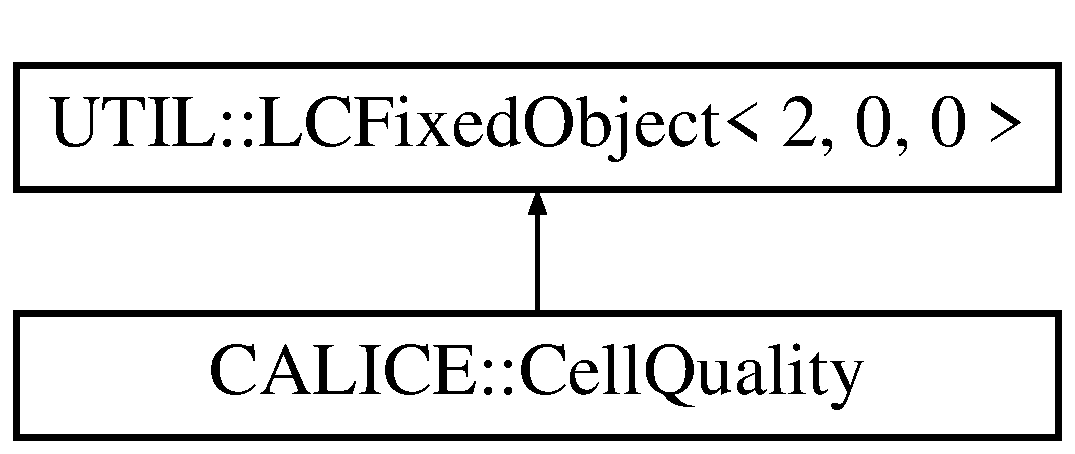
\includegraphics[height=2.000000cm]{classCALICE_1_1CellQuality}
\end{center}
\end{figure}
\subsection*{Public Member Functions}
\begin{DoxyCompactItemize}
\item 
{\bf Cell\-Quality} (const int id, const int status=0)
\begin{DoxyCompactList}\small\item\em Initialise the \doxyref{Cell\-Quality}{p.}{classCALICE_1_1CellQuality} with the Cell\-I\-D. \end{DoxyCompactList}\item 
{\bfseries Cell\-Quality} (E\-V\-E\-N\-T\-::\-L\-C\-Object $\ast$)\label{classCALICE_1_1CellQuality_a67a0a10871b506705a93d15c5c9f1398}

\item 
const int {\bf get\-Cell\-I\-D} () const \label{classCALICE_1_1CellQuality_a5c4b83d65a3e51683c7f1de9609c9cd8}

\begin{DoxyCompactList}\small\item\em Get the cell I\-D. \end{DoxyCompactList}\item 
const int {\bf get\-Status} () const \label{classCALICE_1_1CellQuality_a1ec6dbf56828da5575e9d268632d534d}

\begin{DoxyCompactList}\small\item\em Get the status. \end{DoxyCompactList}\item 
bool {\bf is\-Dead} () const \label{classCALICE_1_1CellQuality_ad886e21dfeb1e49da166a72f5394baa5}

\begin{DoxyCompactList}\small\item\em Check if the cell has been marked as dead. \end{DoxyCompactList}\item 
bool {\bf is\-Noisy} () const \label{classCALICE_1_1CellQuality_a7c90423f24c3c29bb8b1d7ab2d612f02}

\begin{DoxyCompactList}\small\item\em Check if the cell has been marked as noisy. \end{DoxyCompactList}\item 
void {\bf set\-Dead} (bool dead=true)\label{classCALICE_1_1CellQuality_a009ab8aa42248bfad012b8583dad272a}

\begin{DoxyCompactList}\small\item\em Set the dead flag. By using {\ttfamily set\-Dead(false)} you can unset the dead status. \end{DoxyCompactList}\item 
void {\bf set\-Noisy} (bool noisy=true)\label{classCALICE_1_1CellQuality_a116fcb57a8e8c0de606b30c62fb3a46c}

\begin{DoxyCompactList}\small\item\em Set the noisy flag. By using {\ttfamily set\-Noisy(false)} you can unset the noisy status. \end{DoxyCompactList}\item 
virtual const std\-::string {\bfseries get\-Type\-Name} () const \label{classCALICE_1_1CellQuality_a016d2d5250c6bdb0163f65e346e0aa38}

\item 
virtual const std\-::string {\bfseries get\-Data\-Description} () const \label{classCALICE_1_1CellQuality_ade0507fb47735c097963655f99ec87eb}

\end{DoxyCompactItemize}
\subsection*{Static Protected Attributes}
\begin{DoxyCompactItemize}
\item 
static const int {\bf \-\_\-dead} = 0x1\label{classCALICE_1_1CellQuality_a678fd1b8a9b414839b46336c345d642c}

\begin{DoxyCompactList}\small\item\em the dead bit\-: 0x1 \end{DoxyCompactList}\item 
static const int {\bf \-\_\-noisy} = 0x2\label{classCALICE_1_1CellQuality_a46bbb8d66e2ac749976f7a4bffbe4df6}

\begin{DoxyCompactList}\small\item\em the noisy bit\-: 0x2 \end{DoxyCompactList}\end{DoxyCompactItemize}
\subsection*{Private Member Functions}
\begin{DoxyCompactItemize}
\item 
void {\bf set\-Status} (int status)
\begin{DoxyCompactList}\small\item\em The setting of the status is private. \end{DoxyCompactList}\end{DoxyCompactItemize}


\subsection{Detailed Description}
L\-C\-I\-O contions data class to describe the cell quality. 

The cell can be dead or noisy (or both, for instance if a cell is noisy and then dies during a run period).

Note\-: Internally the status is treated as a bit pattern, which allows setting several flags simulaneously and can easily be extended. Thanks to the user interface the user never has to fiddle around with the bits. The definition is protected inside the class and queried with \doxyref{is\-Dead()}{p.}{classCALICE_1_1CellQuality_ad886e21dfeb1e49da166a72f5394baa5} or \doxyref{is\-Noisy()}{p.}{classCALICE_1_1CellQuality_a7c90423f24c3c29bb8b1d7ab2d612f02}.

\begin{DoxyAuthor}{Author}
Niels Meyer, Desy 

Martin Killenberg, C\-E\-R\-N 
\end{DoxyAuthor}


Definition at line 23 of file Cell\-Quality.\-hh.



\subsection{Constructor \& Destructor Documentation}
\index{C\-A\-L\-I\-C\-E\-::\-Cell\-Quality@{C\-A\-L\-I\-C\-E\-::\-Cell\-Quality}!Cell\-Quality@{Cell\-Quality}}
\index{Cell\-Quality@{Cell\-Quality}!CALICE::CellQuality@{C\-A\-L\-I\-C\-E\-::\-Cell\-Quality}}
\subsubsection[{Cell\-Quality}]{\setlength{\rightskip}{0pt plus 5cm}C\-A\-L\-I\-C\-E\-::\-Cell\-Quality\-::\-Cell\-Quality (
\begin{DoxyParamCaption}
\item[{const int}]{id, }
\item[{const int}]{status = {\ttfamily 0}}
\end{DoxyParamCaption}
)}\label{classCALICE_1_1CellQuality_adcbec5052d671a6784ea785bb1521d79}


Initialise the \doxyref{Cell\-Quality}{p.}{classCALICE_1_1CellQuality} with the Cell\-I\-D. 

When the status is already know it can also be given to the constructor (optional). 

Definition at line 11 of file Cell\-Quality.\-cc.



References set\-Status().



\subsection{Member Function Documentation}
\index{C\-A\-L\-I\-C\-E\-::\-Cell\-Quality@{C\-A\-L\-I\-C\-E\-::\-Cell\-Quality}!set\-Status@{set\-Status}}
\index{set\-Status@{set\-Status}!CALICE::CellQuality@{C\-A\-L\-I\-C\-E\-::\-Cell\-Quality}}
\subsubsection[{set\-Status}]{\setlength{\rightskip}{0pt plus 5cm}void C\-A\-L\-I\-C\-E\-::\-Cell\-Quality\-::set\-Status (
\begin{DoxyParamCaption}
\item[{int}]{status}
\end{DoxyParamCaption}
)\hspace{0.3cm}{\ttfamily [private]}}\label{classCALICE_1_1CellQuality_a96b044851c3c6c3d7526291ad005a6bf}


The setting of the status is private. 

It is only allowed using the conctructor or the set() functions. 

Definition at line 19 of file Cell\-Quality.\-cc.



Referenced by Cell\-Quality(), set\-Dead(), and set\-Noisy().



The documentation for this class was generated from the following files\-:\begin{DoxyCompactItemize}
\item 
Cell\-Quality.\-hh\item 
Cell\-Quality.\-cc\end{DoxyCompactItemize}

\section{C\-A\-L\-I\-C\-E\-:\-:Cluster\-Shapes\-Typed Class Reference}
\label{classCALICE_1_1ClusterShapesTyped}\index{C\-A\-L\-I\-C\-E\-::\-Cluster\-Shapes\-Typed@{C\-A\-L\-I\-C\-E\-::\-Cluster\-Shapes\-Typed}}
\subsection*{Public Member Functions}
\begin{DoxyCompactItemize}
\item 
{\footnotesize template$<$class T $>$ }\\void {\bfseries fill} (const lcio\-::\-L\-C\-Collection $\ast$col)\label{classCALICE_1_1ClusterShapesTyped_a4e83529f57aab8f0c3ba1a014868e861}

\item 
Cluster\-Shapes $\ast$ {\bfseries get\-Cluster\-Shapes\-Pointer} ()\label{classCALICE_1_1ClusterShapesTyped_a856df7a286fb0facfd9a87ae11286ec9}

\item 
Cluster\-Shapes $\ast$$\ast$ {\bfseries get\-Cluster\-Shapes\-Pointer\-Pointer} ()\label{classCALICE_1_1ClusterShapesTyped_a9d3fabcc3aebb217c7c5673c077bb4ea}

\end{DoxyCompactItemize}
\subsection*{Private Member Functions}
\begin{DoxyCompactItemize}
\item 
void {\bfseries generate\-Shapes} ()\label{classCALICE_1_1ClusterShapesTyped_a0526e8ad7d133ee4b3fee30d13f72d66}

\end{DoxyCompactItemize}
\subsection*{Private Attributes}
\begin{DoxyCompactItemize}
\item 
Cluster\-Shapes $\ast$ {\bfseries \-\_\-shapes}\label{classCALICE_1_1ClusterShapesTyped_abefd2921e7b46295049038249a341e0c}

\item 
Cluster\-Shapes $\ast$$\ast$ {\bfseries \-\_\-shapes\-Pointer}\label{classCALICE_1_1ClusterShapesTyped_ab876f0147f6c5637461214d6373ba5ab}

\item 
std\-::vector$<$ float $>$ {\bfseries \-\_\-a\-Hit}\label{classCALICE_1_1ClusterShapesTyped_aa04563ae806937cc66e2ea67c7793449}

\item 
std\-::vector$<$ float $>$ {\bfseries \-\_\-x\-Hit}\label{classCALICE_1_1ClusterShapesTyped_a4392fd32a786c63115624cb82218c509}

\item 
std\-::vector$<$ float $>$ {\bfseries \-\_\-y\-Hit}\label{classCALICE_1_1ClusterShapesTyped_ac7e0b672703cd19d2327a774d2472bf7}

\item 
std\-::vector$<$ float $>$ {\bfseries \-\_\-z\-Hit}\label{classCALICE_1_1ClusterShapesTyped_acd58104f72c22a4d34b3455c17fc361c}

\end{DoxyCompactItemize}


\subsection{Detailed Description}


Definition at line 10 of file Cluster\-Shapes\-Typed.\-hh.



The documentation for this class was generated from the following file\-:\begin{DoxyCompactItemize}
\item 
Cluster\-Shapes\-Typed.\-hh\end{DoxyCompactItemize}

\section{C\-A\-L\-I\-C\-E\-:\-:Conditions\-Change\-Delegator$<$ T $>$ Class Template Reference}
\label{classCALICE_1_1ConditionsChangeDelegator}\index{C\-A\-L\-I\-C\-E\-::\-Conditions\-Change\-Delegator$<$ T $>$@{C\-A\-L\-I\-C\-E\-::\-Conditions\-Change\-Delegator$<$ T $>$}}


Listens for conditions data changes and delegates the information to a class.  




{\ttfamily \#include $<$Conditions\-Change\-Delegator.\-hh$>$}

Inheritance diagram for C\-A\-L\-I\-C\-E\-:\-:Conditions\-Change\-Delegator$<$ T $>$\-:\begin{figure}[H]
\begin{center}
\leavevmode
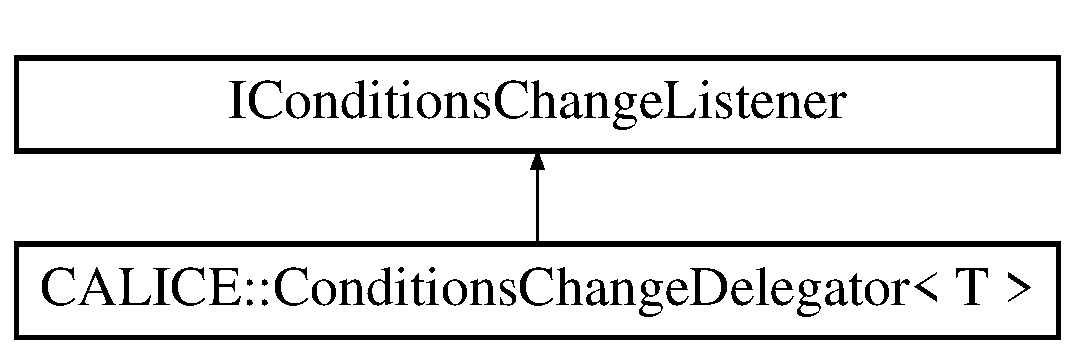
\includegraphics[height=2.000000cm]{classCALICE_1_1ConditionsChangeDelegator}
\end{center}
\end{figure}
\subsection*{Public Types}
\begin{DoxyCompactItemize}
\item 
typedef void(T\-::$\ast$ {\bfseries Conditions\-Change\-Handle\-Func\-\_\-t} )(lcio\-::\-L\-C\-Collection $\ast$col)\label{classCALICE_1_1ConditionsChangeDelegator_afd68318ab8917fd1f97d18ae8204c167}

\end{DoxyCompactItemize}
\subsection*{Public Member Functions}
\begin{DoxyCompactItemize}
\item 
{\bfseries Conditions\-Change\-Delegator} (T $\ast$responsible, Conditions\-Change\-Handle\-Func\-\_\-t a\-\_\-func)\label{classCALICE_1_1ConditionsChangeDelegator_a724d008ad96b77fa64b8716545052b57}

\item 
void {\bf conditions\-Changed} (lcio\-::\-L\-C\-Collection $\ast$col)
\begin{DoxyCompactList}\small\item\em Be notified if conditions data changes and redirect changes to responsible class. \end{DoxyCompactList}\end{DoxyCompactItemize}
\subsection*{Private Attributes}
\begin{DoxyCompactItemize}
\item 
Conditions\-Change\-Handle\-Func\-\_\-t {\bf \-\_\-func\-P}\label{classCALICE_1_1ConditionsChangeDelegator_adaf17b9ce91ac651de46c007b69f5719}

\begin{DoxyCompactList}\small\item\em method to be called if the conditions data changed \end{DoxyCompactList}\item 
T $\ast$ {\bf \-\_\-responsible}\label{classCALICE_1_1ConditionsChangeDelegator_a0d8f29b22856a229930ee6246ad066fd}

\begin{DoxyCompactList}\small\item\em the object which will take care of the change \end{DoxyCompactList}\end{DoxyCompactItemize}


\subsection{Detailed Description}
\subsubsection*{template$<$class T$>$class C\-A\-L\-I\-C\-E\-::\-Conditions\-Change\-Delegator$<$ T $>$}

Listens for conditions data changes and delegates the information to a class. 

a class can redirect several conditions data changes to itself. \begin{DoxySeeAlso}{See Also}
test\-Conditions\-Data\-Delegator.\-cc 
\end{DoxySeeAlso}


Definition at line 13 of file Conditions\-Change\-Delegator.\-hh.



\subsection{Member Function Documentation}
\index{C\-A\-L\-I\-C\-E\-::\-Conditions\-Change\-Delegator@{C\-A\-L\-I\-C\-E\-::\-Conditions\-Change\-Delegator}!conditions\-Changed@{conditions\-Changed}}
\index{conditions\-Changed@{conditions\-Changed}!CALICE::ConditionsChangeDelegator@{C\-A\-L\-I\-C\-E\-::\-Conditions\-Change\-Delegator}}
\subsubsection[{conditions\-Changed}]{\setlength{\rightskip}{0pt plus 5cm}template$<$class T$>$ void {\bf C\-A\-L\-I\-C\-E\-::\-Conditions\-Change\-Delegator}$<$ T $>$\-::conditions\-Changed (
\begin{DoxyParamCaption}
\item[{lcio\-::\-L\-C\-Collection $\ast$}]{col}
\end{DoxyParamCaption}
)\hspace{0.3cm}{\ttfamily [inline]}}\label{classCALICE_1_1ConditionsChangeDelegator_a4eae95674a704dd8d59a6fb4ca1490ea}


Be notified if conditions data changes and redirect changes to responsible class. 


\begin{DoxyParams}{Parameters}
{\em col} & the collection containing the new conditions data \\
\hline
\end{DoxyParams}


Definition at line 26 of file Conditions\-Change\-Delegator.\-hh.



The documentation for this class was generated from the following file\-:\begin{DoxyCompactItemize}
\item 
Conditions\-Change\-Delegator.\-hh\end{DoxyCompactItemize}

\section{C\-A\-L\-I\-C\-E\-:\-:Conditions\-Data\-Write\-Handler Class Reference}
\label{classCALICE_1_1ConditionsDataWriteHandler}\index{C\-A\-L\-I\-C\-E\-::\-Conditions\-Data\-Write\-Handler@{C\-A\-L\-I\-C\-E\-::\-Conditions\-Data\-Write\-Handler}}


Handler of conditions data changes which writes the replaced collections to a conditions data base.  




{\ttfamily \#include $<$Conditions\-Data\-Write\-Handler.\-hh$>$}

Inheritance diagram for C\-A\-L\-I\-C\-E\-:\-:Conditions\-Data\-Write\-Handler\-:\begin{figure}[H]
\begin{center}
\leavevmode
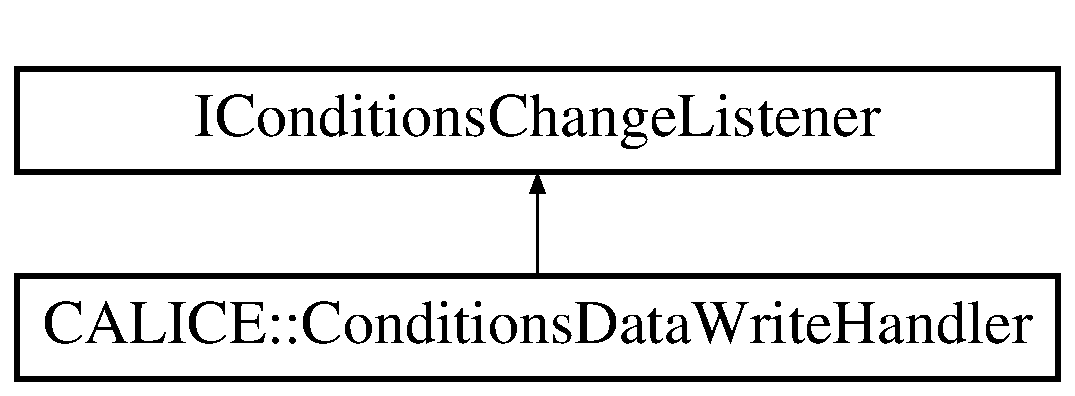
\includegraphics[height=2.000000cm]{classCALICE_1_1ConditionsDataWriteHandler}
\end{center}
\end{figure}
\subsection*{Public Member Functions}
\begin{DoxyCompactItemize}
\item 
{\bf Conditions\-Data\-Write\-Handler} (const std\-::string \&col\-\_\-name, const std\-::string \&db\-\_\-init\-\_\-string, const std\-::string \&folder\-\_\-name, const std\-::string \&tag, const std\-::string \&description)
\begin{DoxyCompactList}\small\item\em constructor. \end{DoxyCompactList}\item 
{\bf $\sim$\-Conditions\-Data\-Write\-Handler} ()\label{classCALICE_1_1ConditionsDataWriteHandler_a581dea40c8faa28948c8cb461d9126dc}

\begin{DoxyCompactList}\small\item\em destructor. \end{DoxyCompactList}\item 
void {\bf conditions\-Changed} (lcio\-::\-L\-C\-Collection $\ast$col)
\begin{DoxyCompactList}\small\item\em Be notified if conditions data changes and redirect changes to responsible class. \end{DoxyCompactList}\item 
void {\bf write\-Conditions\-Data} (const long64 \&best\-\_\-guess\-\_\-of\-\_\-till\-\_\-time\-\_\-stamp)
\begin{DoxyCompactList}\small\item\em write the conditions data to the conditions database. \end{DoxyCompactList}\item 
void {\bf set\-Since\-Time} (long64 since\-\_\-time)
\begin{DoxyCompactList}\small\item\em Set the correct since time for the current conditions data. \end{DoxyCompactList}\item 
const std\-::string \& {\bfseries name} () const \label{classCALICE_1_1ConditionsDataWriteHandler_a578e53e8c53ee791d1ab574811551496}

\item 
unsigned int {\bf number\-Of\-Writes} () const \label{classCALICE_1_1ConditionsDataWriteHandler_a535ca783c3475b0cbacd99484c4e4229}

\begin{DoxyCompactList}\small\item\em Get the number of collections written to the database;. \end{DoxyCompactList}\item 
unsigned int {\bf changes} () const \label{classCALICE_1_1ConditionsDataWriteHandler_ae53d14eec368dc28b8bc5dcb73ed2d01}

\begin{DoxyCompactList}\small\item\em Get the number of recognised changes of the conditions data. \end{DoxyCompactList}\item 
long64 {\bf valid\-At\-Most\-Since} () const \label{classCALICE_1_1ConditionsDataWriteHandler_a1899ab4669280acec16c6baa53e6abc3}

\begin{DoxyCompactList}\small\item\em Get the time of the first recognised conditions data change. \end{DoxyCompactList}\item 
long64 {\bf valid\-At\-Most\-Till} () const \label{classCALICE_1_1ConditionsDataWriteHandler_a487fe71c6d796b46dac6dd7ea16eb917}

\begin{DoxyCompactList}\small\item\em Get the time of the last write to the data base. \end{DoxyCompactList}\item 
long64 {\bf current\-Valid\-Since} () const \label{classCALICE_1_1ConditionsDataWriteHandler_ac3a420cb581ed9519e06e795dd13ac9a}

\begin{DoxyCompactList}\small\item\em Get the time of the first recognised conditions data change. \end{DoxyCompactList}\item 
long64 {\bf current\-Valid\-Till} () const \label{classCALICE_1_1ConditionsDataWriteHandler_a7cae6dc5fd78a5aa243bb589ba4c7caa}

\begin{DoxyCompactList}\small\item\em Get the time of the last write to the data base. \end{DoxyCompactList}\item 
const std\-::string \& {\bfseries get\-Tag} () const \label{classCALICE_1_1ConditionsDataWriteHandler_a3e14961a4bf03b6282f2b59fe87790fa}

\end{DoxyCompactItemize}
\subsection*{Private Attributes}
\begin{DoxyCompactItemize}
\item 
const std\-::string {\bf \-\_\-col\-Name}\label{classCALICE_1_1ConditionsDataWriteHandler_a7e065bb6ab09b579ce20f7dbbbdf07a2}

\begin{DoxyCompactList}\small\item\em name of the collection (not used) \end{DoxyCompactList}\item 
lccd\-::\-D\-B\-Interface {\bfseries \-\_\-db}\label{classCALICE_1_1ConditionsDataWriteHandler_a94ae745611b1bff4441eab7677c408c1}

\item 
lccd\-::\-I\-Conditions\-Handler $\ast$ {\bf \-\_\-change\-Handler}\label{classCALICE_1_1ConditionsDataWriteHandler_a3a20bce4a053386c2d4f786653438f38}

\begin{DoxyCompactList}\small\item\em handler of the conditions data \end{DoxyCompactList}\item 
const std\-::string {\bfseries \-\_\-tag}\label{classCALICE_1_1ConditionsDataWriteHandler_a62de4dca742011f4fdb976d4bb3abee2}

\item 
const std\-::string {\bfseries \-\_\-description}\label{classCALICE_1_1ConditionsDataWriteHandler_a01342556e5b2c4916dbb3d3705dd0af3}

\item 
long64 {\bf \-\_\-since}
\begin{DoxyCompactList}\small\item\em the time of the event just before the conditions data changed. \end{DoxyCompactList}\item 
long64 {\bf \-\_\-till}
\begin{DoxyCompactList}\small\item\em Best guess of the till time stamp (may be wrong). \end{DoxyCompactList}\item 
L\-C\-Collection $\ast$ {\bf \-\_\-col}
\begin{DoxyCompactList}\small\item\em pointer to the clone of the conditions data collection. \end{DoxyCompactList}\item 
unsigned int {\bf \-\_\-changes}
\begin{DoxyCompactList}\small\item\em keep track of the number of changes. \end{DoxyCompactList}\item 
unsigned int {\bf \-\_\-writes}
\begin{DoxyCompactList}\small\item\em keep track of the number of conditions data written to the database. \end{DoxyCompactList}\item 
long64 {\bfseries \-\_\-first}\label{classCALICE_1_1ConditionsDataWriteHandler_a8076fe1b19e269527fa769de5a88a65e}

\item 
long64 {\bfseries \-\_\-last}\label{classCALICE_1_1ConditionsDataWriteHandler_a5debaace61a41f99d2df0ce318c036bf}

\end{DoxyCompactItemize}


\subsection{Detailed Description}
Handler of conditions data changes which writes the replaced collections to a conditions data base. 

When ever conditions data changes the old (cloned) collection will be stored with the time stamps of the event just before the former conditions data change and the time stamp of the last event. At the end of the run, the conditions data has to be written manually by calling \doxyref{write\-Conditions\-Data()}{p.}{classCALICE_1_1ConditionsDataWriteHandler_a139623a650f56c24a5d32658da9af09b} with the time stamp of the last event. 

Definition at line 40 of file Conditions\-Data\-Write\-Handler.\-hh.



\subsection{Constructor \& Destructor Documentation}
\index{C\-A\-L\-I\-C\-E\-::\-Conditions\-Data\-Write\-Handler@{C\-A\-L\-I\-C\-E\-::\-Conditions\-Data\-Write\-Handler}!Conditions\-Data\-Write\-Handler@{Conditions\-Data\-Write\-Handler}}
\index{Conditions\-Data\-Write\-Handler@{Conditions\-Data\-Write\-Handler}!CALICE::ConditionsDataWriteHandler@{C\-A\-L\-I\-C\-E\-::\-Conditions\-Data\-Write\-Handler}}
\subsubsection[{Conditions\-Data\-Write\-Handler}]{\setlength{\rightskip}{0pt plus 5cm}C\-A\-L\-I\-C\-E\-::\-Conditions\-Data\-Write\-Handler\-::\-Conditions\-Data\-Write\-Handler (
\begin{DoxyParamCaption}
\item[{const std\-::string \&}]{col\-\_\-name, }
\item[{const std\-::string \&}]{db\-\_\-init\-\_\-string, }
\item[{const std\-::string \&}]{folder\-\_\-name, }
\item[{const std\-::string \&}]{tag, }
\item[{const std\-::string \&}]{description}
\end{DoxyParamCaption}
)}\label{classCALICE_1_1ConditionsDataWriteHandler_ae0e0b43ca010d9a424f962480175b110}


constructor. 


\begin{DoxyParams}{Parameters}
{\em col\-\_\-name} & the name of the to be monitored collection (not needed). \\
\hline
{\em db\-\_\-init\-\_\-string} & specifier of the database host name, database name, user and password. \\
\hline
{\em folder\-\_\-name} & name of the destination folder. \\
\hline
{\em tag} & to be applied at the end of the run to the folder. \\
\hline
{\em description} & the description added to every collection written toe the data base. \\
\hline
\end{DoxyParams}


Definition at line 15 of file Conditions\-Data\-Write\-Handler.\-cc.



References \-\_\-change\-Handler, \-\_\-col\-Name, \-\_\-since, and \-\_\-till.



\subsection{Member Function Documentation}
\index{C\-A\-L\-I\-C\-E\-::\-Conditions\-Data\-Write\-Handler@{C\-A\-L\-I\-C\-E\-::\-Conditions\-Data\-Write\-Handler}!conditions\-Changed@{conditions\-Changed}}
\index{conditions\-Changed@{conditions\-Changed}!CALICE::ConditionsDataWriteHandler@{C\-A\-L\-I\-C\-E\-::\-Conditions\-Data\-Write\-Handler}}
\subsubsection[{conditions\-Changed}]{\setlength{\rightskip}{0pt plus 5cm}void C\-A\-L\-I\-C\-E\-::\-Conditions\-Data\-Write\-Handler\-::conditions\-Changed (
\begin{DoxyParamCaption}
\item[{lcio\-::\-L\-C\-Collection $\ast$}]{col}
\end{DoxyParamCaption}
)}\label{classCALICE_1_1ConditionsDataWriteHandler_a0289e54f162d87125bce02b71dc46b51}


Be notified if conditions data changes and redirect changes to responsible class. 


\begin{DoxyParams}{Parameters}
{\em col} & the collection containing the new conditions data \\
\hline
\end{DoxyParams}
if (\-\_\-change\-Handler) \{ 

Definition at line 59 of file Conditions\-Data\-Write\-Handler.\-cc.



References \-\_\-change\-Handler, \-\_\-changes, \-\_\-col, \-\_\-col\-Name, \-\_\-since, \-\_\-till, C\-A\-L\-I\-C\-E\-::clone\-Collection(), and write\-Conditions\-Data().

\index{C\-A\-L\-I\-C\-E\-::\-Conditions\-Data\-Write\-Handler@{C\-A\-L\-I\-C\-E\-::\-Conditions\-Data\-Write\-Handler}!set\-Since\-Time@{set\-Since\-Time}}
\index{set\-Since\-Time@{set\-Since\-Time}!CALICE::ConditionsDataWriteHandler@{C\-A\-L\-I\-C\-E\-::\-Conditions\-Data\-Write\-Handler}}
\subsubsection[{set\-Since\-Time}]{\setlength{\rightskip}{0pt plus 5cm}void C\-A\-L\-I\-C\-E\-::\-Conditions\-Data\-Write\-Handler\-::set\-Since\-Time (
\begin{DoxyParamCaption}
\item[{long64}]{since\-\_\-time}
\end{DoxyParamCaption}
)\hspace{0.3cm}{\ttfamily [inline]}}\label{classCALICE_1_1ConditionsDataWriteHandler_aaac4f4263bbfb7a38cfbf0cb6c6ef99b}


Set the correct since time for the current conditions data. 

The since time will be initialised by the time of the last event. But this is just too early. So, the \doxyref{marlin\-::\-Conditions\-Data\-Writer}{p.}{classmarlin_1_1ConditionsDataWriter} has to set the time of the next event. 

Definition at line 78 of file Conditions\-Data\-Write\-Handler.\-hh.



References \-\_\-since.

\index{C\-A\-L\-I\-C\-E\-::\-Conditions\-Data\-Write\-Handler@{C\-A\-L\-I\-C\-E\-::\-Conditions\-Data\-Write\-Handler}!write\-Conditions\-Data@{write\-Conditions\-Data}}
\index{write\-Conditions\-Data@{write\-Conditions\-Data}!CALICE::ConditionsDataWriteHandler@{C\-A\-L\-I\-C\-E\-::\-Conditions\-Data\-Write\-Handler}}
\subsubsection[{write\-Conditions\-Data}]{\setlength{\rightskip}{0pt plus 5cm}void C\-A\-L\-I\-C\-E\-::\-Conditions\-Data\-Write\-Handler\-::write\-Conditions\-Data (
\begin{DoxyParamCaption}
\item[{const long64 \&}]{best\-\_\-guess\-\_\-of\-\_\-till\-\_\-time\-\_\-stamp}
\end{DoxyParamCaption}
)}\label{classCALICE_1_1ConditionsDataWriteHandler_a139623a650f56c24a5d32658da9af09b}


write the conditions data to the conditions database. 

Must be called at the end of the run to 

Definition at line 112 of file Conditions\-Data\-Write\-Handler.\-cc.



References \-\_\-col, \-\_\-col\-Name, \-\_\-since, and \-\_\-writes.



Referenced by conditions\-Changed().



\subsection{Field Documentation}
\index{C\-A\-L\-I\-C\-E\-::\-Conditions\-Data\-Write\-Handler@{C\-A\-L\-I\-C\-E\-::\-Conditions\-Data\-Write\-Handler}!\-\_\-changes@{\-\_\-changes}}
\index{\-\_\-changes@{\-\_\-changes}!CALICE::ConditionsDataWriteHandler@{C\-A\-L\-I\-C\-E\-::\-Conditions\-Data\-Write\-Handler}}
\subsubsection[{\-\_\-changes}]{\setlength{\rightskip}{0pt plus 5cm}unsigned int C\-A\-L\-I\-C\-E\-::\-Conditions\-Data\-Write\-Handler\-::\-\_\-changes\hspace{0.3cm}{\ttfamily [private]}}\label{classCALICE_1_1ConditionsDataWriteHandler_a3f95dd0e4ec24fbd1d4df217a679191d}


keep track of the number of changes. 



Definition at line 124 of file Conditions\-Data\-Write\-Handler.\-hh.



Referenced by conditions\-Changed().

\index{C\-A\-L\-I\-C\-E\-::\-Conditions\-Data\-Write\-Handler@{C\-A\-L\-I\-C\-E\-::\-Conditions\-Data\-Write\-Handler}!\-\_\-col@{\-\_\-col}}
\index{\-\_\-col@{\-\_\-col}!CALICE::ConditionsDataWriteHandler@{C\-A\-L\-I\-C\-E\-::\-Conditions\-Data\-Write\-Handler}}
\subsubsection[{\-\_\-col}]{\setlength{\rightskip}{0pt plus 5cm}L\-C\-Collection$\ast$ C\-A\-L\-I\-C\-E\-::\-Conditions\-Data\-Write\-Handler\-::\-\_\-col\hspace{0.3cm}{\ttfamily [private]}}\label{classCALICE_1_1ConditionsDataWriteHandler_a8db218626a224e54f964cf46054890cb}


pointer to the clone of the conditions data collection. 



Definition at line 121 of file Conditions\-Data\-Write\-Handler.\-hh.



Referenced by conditions\-Changed(), write\-Conditions\-Data(), and $\sim$\-Conditions\-Data\-Write\-Handler().

\index{C\-A\-L\-I\-C\-E\-::\-Conditions\-Data\-Write\-Handler@{C\-A\-L\-I\-C\-E\-::\-Conditions\-Data\-Write\-Handler}!\-\_\-since@{\-\_\-since}}
\index{\-\_\-since@{\-\_\-since}!CALICE::ConditionsDataWriteHandler@{C\-A\-L\-I\-C\-E\-::\-Conditions\-Data\-Write\-Handler}}
\subsubsection[{\-\_\-since}]{\setlength{\rightskip}{0pt plus 5cm}long64 C\-A\-L\-I\-C\-E\-::\-Conditions\-Data\-Write\-Handler\-::\-\_\-since\hspace{0.3cm}{\ttfamily [private]}}\label{classCALICE_1_1ConditionsDataWriteHandler_ae9c2172504130f906f18d6459823d62b}


the time of the event just before the conditions data changed. 



Definition at line 119 of file Conditions\-Data\-Write\-Handler.\-hh.



Referenced by conditions\-Changed(), Conditions\-Data\-Write\-Handler(), current\-Valid\-Since(), set\-Since\-Time(), and write\-Conditions\-Data().

\index{C\-A\-L\-I\-C\-E\-::\-Conditions\-Data\-Write\-Handler@{C\-A\-L\-I\-C\-E\-::\-Conditions\-Data\-Write\-Handler}!\-\_\-till@{\-\_\-till}}
\index{\-\_\-till@{\-\_\-till}!CALICE::ConditionsDataWriteHandler@{C\-A\-L\-I\-C\-E\-::\-Conditions\-Data\-Write\-Handler}}
\subsubsection[{\-\_\-till}]{\setlength{\rightskip}{0pt plus 5cm}long64 C\-A\-L\-I\-C\-E\-::\-Conditions\-Data\-Write\-Handler\-::\-\_\-till\hspace{0.3cm}{\ttfamily [private]}}\label{classCALICE_1_1ConditionsDataWriteHandler_a3867ef683d994f3ab4a00b2ef7ae410c}


Best guess of the till time stamp (may be wrong). 



Definition at line 120 of file Conditions\-Data\-Write\-Handler.\-hh.



Referenced by conditions\-Changed(), Conditions\-Data\-Write\-Handler(), and current\-Valid\-Till().

\index{C\-A\-L\-I\-C\-E\-::\-Conditions\-Data\-Write\-Handler@{C\-A\-L\-I\-C\-E\-::\-Conditions\-Data\-Write\-Handler}!\-\_\-writes@{\-\_\-writes}}
\index{\-\_\-writes@{\-\_\-writes}!CALICE::ConditionsDataWriteHandler@{C\-A\-L\-I\-C\-E\-::\-Conditions\-Data\-Write\-Handler}}
\subsubsection[{\-\_\-writes}]{\setlength{\rightskip}{0pt plus 5cm}unsigned int C\-A\-L\-I\-C\-E\-::\-Conditions\-Data\-Write\-Handler\-::\-\_\-writes\hspace{0.3cm}{\ttfamily [private]}}\label{classCALICE_1_1ConditionsDataWriteHandler_aafdf1c7e91d569aed9cf422cd77d8fb6}


keep track of the number of conditions data written to the database. 



Definition at line 126 of file Conditions\-Data\-Write\-Handler.\-hh.



Referenced by changes(), number\-Of\-Writes(), and write\-Conditions\-Data().



The documentation for this class was generated from the following files\-:\begin{DoxyCompactItemize}
\item 
Conditions\-Data\-Write\-Handler.\-hh\item 
Conditions\-Data\-Write\-Handler.\-cc\end{DoxyCompactItemize}

\section{marlin\-:\-:Conditions\-Data\-Writer Class Reference}
\label{classmarlin_1_1ConditionsDataWriter}\index{marlin\-::\-Conditions\-Data\-Writer@{marlin\-::\-Conditions\-Data\-Writer}}


Marlin processr which catches selected conditions data changes and writes them to the conditions data base.  




{\ttfamily \#include $<$Conditions\-Data\-Writer.\-hh$>$}

Inheritance diagram for marlin\-:\-:Conditions\-Data\-Writer\-:\begin{figure}[H]
\begin{center}
\leavevmode
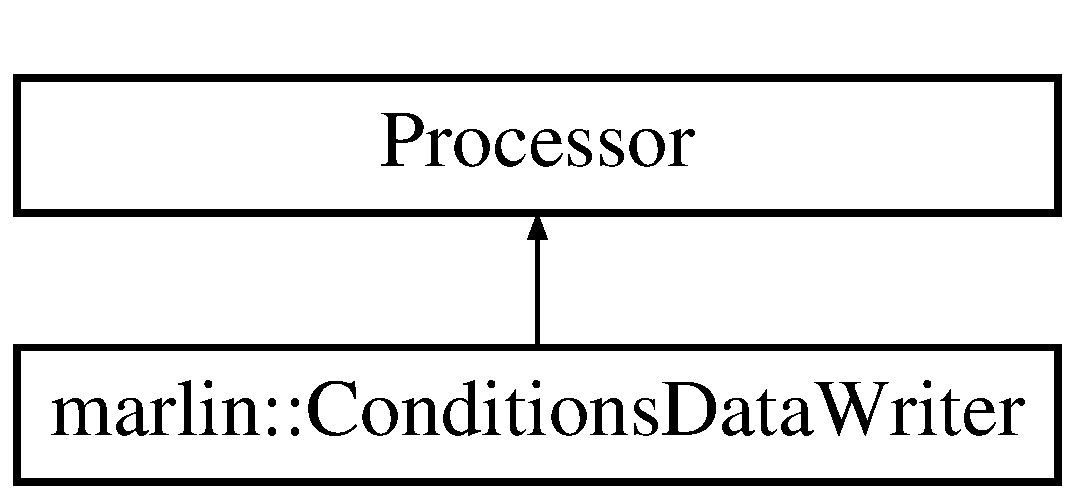
\includegraphics[height=2.000000cm]{classmarlin_1_1ConditionsDataWriter}
\end{center}
\end{figure}
\subsection*{Public Member Functions}
\begin{DoxyCompactItemize}
\item 
Processor $\ast$ {\bfseries new\-Processor} ()\label{classmarlin_1_1ConditionsDataWriter_a360478d5d28f2e5012ef5e0e5201821a}

\item 
void {\bf init} ()
\begin{DoxyCompactList}\small\item\em Install conditions change listener. \end{DoxyCompactList}\item 
void {\bf process\-Run\-Header} (L\-C\-Run\-Header $\ast$run)\label{classmarlin_1_1ConditionsDataWriter_a943dd58f7e315e2ded7f49a77211eb82}

\begin{DoxyCompactList}\small\item\em Do nothing at run start. \end{DoxyCompactList}\item 
void {\bf process\-Event} (L\-C\-Event $\ast$evt\-P)
\begin{DoxyCompactList}\small\item\em Memorise the event time stamps. \end{DoxyCompactList}\item 
void {\bf end} ()
\begin{DoxyCompactList}\small\item\em Write all not yet written conditions data to the conditions data base. \end{DoxyCompactList}\item 
long64 {\bfseries get\-Time\-Stamp\-Of\-Last\-Event} () const \label{classmarlin_1_1ConditionsDataWriter_a8c8683f0e6055c27c991a6f31d5d69a9}

\end{DoxyCompactItemize}
\subsection*{Protected Attributes}
\begin{DoxyCompactItemize}
\item 
std\-::string {\bf \-\_\-db\-Init}
\begin{DoxyCompactList}\small\item\em parameter to be filled with the host name, database name,user name and the password. \end{DoxyCompactList}\item 
String\-Vec {\bf \-\_\-cond\-Data\-Collections}
\begin{DoxyCompactList}\small\item\em collection name, destination Cond\-D\-B folder and version of the conditions data to be written to the conditions database. \end{DoxyCompactList}\item 
long64 {\bf \-\_\-time\-Stamp\-Of\-Last\-Event}
\begin{DoxyCompactList}\small\item\em The time stamp of the last event that was processed. \end{DoxyCompactList}\item 
std\-::vector\\*
$<$ {\bf C\-A\-L\-I\-C\-E\-::\-Conditions\-Data\-Write\-Handler} $\ast$ $>$ {\bfseries \-\_\-handler}\label{classmarlin_1_1ConditionsDataWriter_a68d96e4787ed480558b5b3088cd3321f}

\end{DoxyCompactItemize}
\subsection*{Friends}
\begin{DoxyCompactItemize}
\item 
class {\bfseries C\-A\-L\-I\-C\-E\-::\-Conditions\-Data\-Write\-Handler}\label{classmarlin_1_1ConditionsDataWriter_a0e401bb1bfedeba5808934499877adf4}

\end{DoxyCompactItemize}


\subsection{Detailed Description}
Marlin processr which catches selected conditions data changes and writes them to the conditions data base. 

The processor does not verify whether the data already exists it writes every change to the database.

The conditions data changes are catched by individual handlers which clone the conditions data collection and store the cloned collection when the handler is notified of the next change.

The conditions data change handler does not have any knowledge of the record time which triggered the conditions data change. To solve this problem, the handlers request a correction of the since time stamp. This request will be approximatively fulfilled by setting the since time stamp to the time stamp of the event which arrived just after the conditions data change. 

Definition at line 36 of file Conditions\-Data\-Writer.\-hh.



\subsection{Member Function Documentation}
\index{marlin\-::\-Conditions\-Data\-Writer@{marlin\-::\-Conditions\-Data\-Writer}!end@{end}}
\index{end@{end}!marlin::ConditionsDataWriter@{marlin\-::\-Conditions\-Data\-Writer}}
\subsubsection[{end}]{\setlength{\rightskip}{0pt plus 5cm}void marlin\-::\-Conditions\-Data\-Writer\-::end (
\begin{DoxyParamCaption}
{}
\end{DoxyParamCaption}
)}\label{classmarlin_1_1ConditionsDataWriter_a8ece634cea5d95989d574c128d303006}


Write all not yet written conditions data to the conditions data base. 

The writing of the conditions data is delayed until the conditions data changes to set the \char`\"{}since\char`\"{} and \char`\"{}till\char`\"{} time stamps. All the conditions data which is not yet stored in the conditions database is written now. Finally if the the version is not H\-E\-A\-D, the folders are tagged. 

Definition at line 109 of file Conditions\-Data\-Writer.\-cc.

\index{marlin\-::\-Conditions\-Data\-Writer@{marlin\-::\-Conditions\-Data\-Writer}!init@{init}}
\index{init@{init}!marlin::ConditionsDataWriter@{marlin\-::\-Conditions\-Data\-Writer}}
\subsubsection[{init}]{\setlength{\rightskip}{0pt plus 5cm}void marlin\-::\-Conditions\-Data\-Writer\-::init (
\begin{DoxyParamCaption}
{}
\end{DoxyParamCaption}
)}\label{classmarlin_1_1ConditionsDataWriter_a71c0b9b141b58a82aaf7df60939bf114}


Install conditions change listener. 

The listeners are installed for the conditions data specified by the processor parameters. 

Definition at line 41 of file Conditions\-Data\-Writer.\-cc.

\index{marlin\-::\-Conditions\-Data\-Writer@{marlin\-::\-Conditions\-Data\-Writer}!process\-Event@{process\-Event}}
\index{process\-Event@{process\-Event}!marlin::ConditionsDataWriter@{marlin\-::\-Conditions\-Data\-Writer}}
\subsubsection[{process\-Event}]{\setlength{\rightskip}{0pt plus 5cm}void marlin\-::\-Conditions\-Data\-Writer\-::process\-Event (
\begin{DoxyParamCaption}
\item[{L\-C\-Event $\ast$}]{evt\-P}
\end{DoxyParamCaption}
)}\label{classmarlin_1_1ConditionsDataWriter_afa20ee1d0fcaa87334896a5e5b86920e}


Memorise the event time stamps. 

The time stamp of the last event before the member function end is called is needed to write the dangling conditions data with correct \char`\"{}since\char`\"{} and \char`\"{}till\char`\"{} time stamps to the conditions data base. 

Definition at line 94 of file Conditions\-Data\-Writer.\-cc.



\subsection{Field Documentation}
\index{marlin\-::\-Conditions\-Data\-Writer@{marlin\-::\-Conditions\-Data\-Writer}!\-\_\-cond\-Data\-Collections@{\-\_\-cond\-Data\-Collections}}
\index{\-\_\-cond\-Data\-Collections@{\-\_\-cond\-Data\-Collections}!marlin::ConditionsDataWriter@{marlin\-::\-Conditions\-Data\-Writer}}
\subsubsection[{\-\_\-cond\-Data\-Collections}]{\setlength{\rightskip}{0pt plus 5cm}String\-Vec marlin\-::\-Conditions\-Data\-Writer\-::\-\_\-cond\-Data\-Collections\hspace{0.3cm}{\ttfamily [protected]}}\label{classmarlin_1_1ConditionsDataWriter_aec7c975d8f23f11e20dc1911ce57bb2c}


collection name, destination Cond\-D\-B folder and version of the conditions data to be written to the conditions database. 



Definition at line 77 of file Conditions\-Data\-Writer.\-hh.

\index{marlin\-::\-Conditions\-Data\-Writer@{marlin\-::\-Conditions\-Data\-Writer}!\-\_\-db\-Init@{\-\_\-db\-Init}}
\index{\-\_\-db\-Init@{\-\_\-db\-Init}!marlin::ConditionsDataWriter@{marlin\-::\-Conditions\-Data\-Writer}}
\subsubsection[{\-\_\-db\-Init}]{\setlength{\rightskip}{0pt plus 5cm}std\-::string marlin\-::\-Conditions\-Data\-Writer\-::\-\_\-db\-Init\hspace{0.3cm}{\ttfamily [protected]}}\label{classmarlin_1_1ConditionsDataWriter_ad87dadf50a9e475515ea26bce299e449}


parameter to be filled with the host name, database name,user name and the password. 



Definition at line 72 of file Conditions\-Data\-Writer.\-hh.

\index{marlin\-::\-Conditions\-Data\-Writer@{marlin\-::\-Conditions\-Data\-Writer}!\-\_\-time\-Stamp\-Of\-Last\-Event@{\-\_\-time\-Stamp\-Of\-Last\-Event}}
\index{\-\_\-time\-Stamp\-Of\-Last\-Event@{\-\_\-time\-Stamp\-Of\-Last\-Event}!marlin::ConditionsDataWriter@{marlin\-::\-Conditions\-Data\-Writer}}
\subsubsection[{\-\_\-time\-Stamp\-Of\-Last\-Event}]{\setlength{\rightskip}{0pt plus 5cm}long64 marlin\-::\-Conditions\-Data\-Writer\-::\-\_\-time\-Stamp\-Of\-Last\-Event\hspace{0.3cm}{\ttfamily [protected]}}\label{classmarlin_1_1ConditionsDataWriter_af2c6e1b189e2f665f8ef6beb7ad9c10b}


The time stamp of the last event that was processed. 



Definition at line 80 of file Conditions\-Data\-Writer.\-hh.



The documentation for this class was generated from the following files\-:\begin{DoxyCompactItemize}
\item 
Conditions\-Data\-Writer.\-hh\item 
Conditions\-Data\-Writer.\-cc\end{DoxyCompactItemize}

\section{Conf\-Stat\-\_\-t Class Reference}
\label{classConfStat__t}\index{Conf\-Stat\-\_\-t@{Conf\-Stat\-\_\-t}}


Statistics about configuration record errors.  




{\ttfamily \#include $<$Conf\-Stat\-List\-\_\-t.\-hh$>$}

Inheritance diagram for Conf\-Stat\-\_\-t\-:\begin{figure}[H]
\begin{center}
\leavevmode
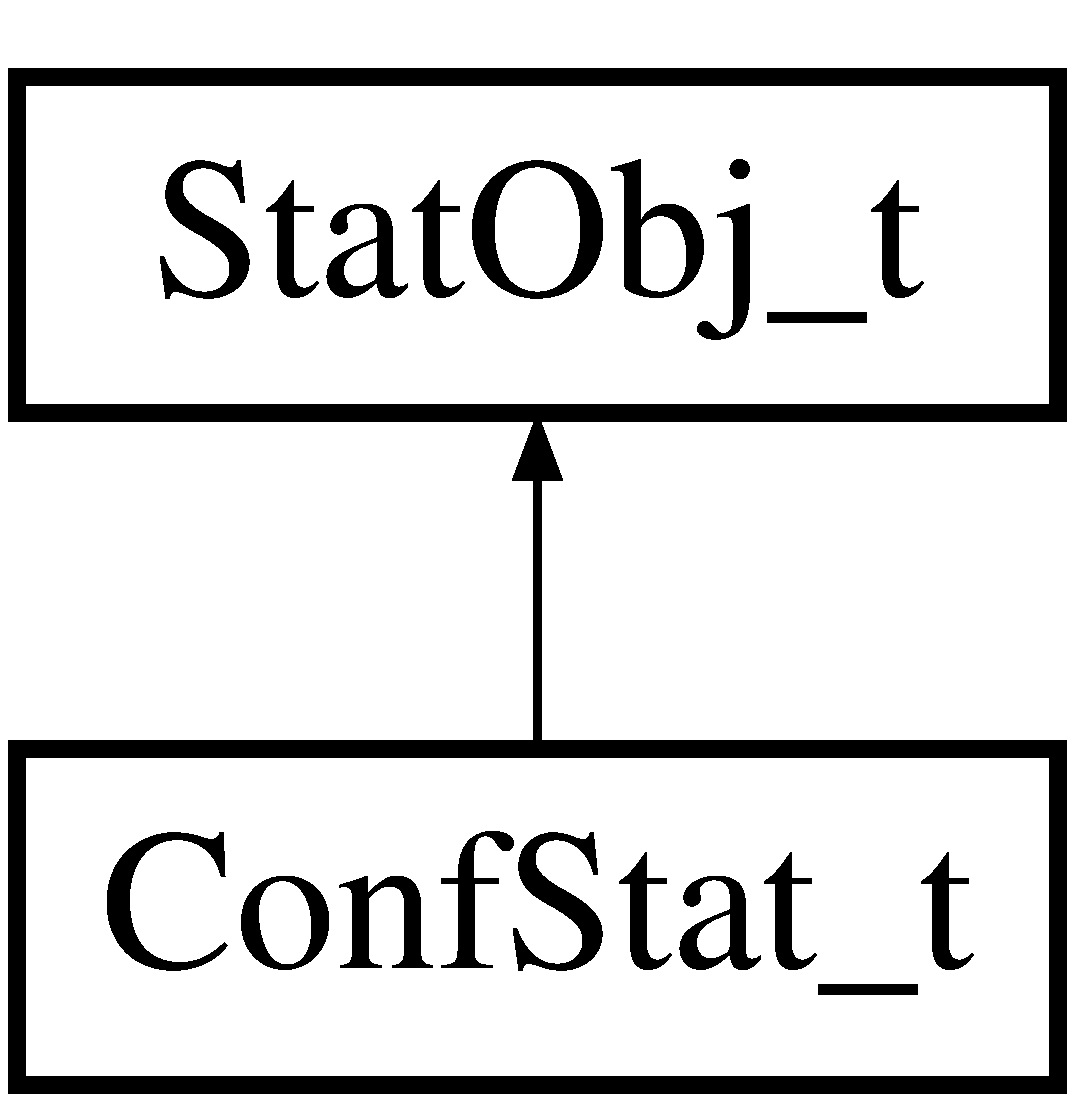
\includegraphics[height=2.000000cm]{classConfStat__t}
\end{center}
\end{figure}
\subsection*{Public Member Functions}
\begin{DoxyCompactItemize}
\item 
void {\bf finish} ()\label{classConfStat__t_a3856ab4b30f39391169a31c27ae15e08}

\begin{DoxyCompactList}\small\item\em Add statistics of the last 10 records. \end{DoxyCompactList}\item 
void {\bf print\-Table\-Header} (std\-::ostream \&out) const \label{classConfStat__t_a26c1d1503dab552f275584065a39e64e}

\begin{DoxyCompactList}\small\item\em Print the table header. \end{DoxyCompactList}\item 
void {\bf print} (std\-::ostream \&out)
\begin{DoxyCompactList}\small\item\em Print the statistics of one object (one table row). \end{DoxyCompactList}\item 
bool {\bf has\-Info} () const 
\begin{DoxyCompactList}\small\item\em Return true if at least one error was detected for the corresponding front-\/end. \end{DoxyCompactList}\item 
void {\bf add\-Good} ()
\begin{DoxyCompactList}\small\item\em The configuration data of the corresponding front-\/end is okay. \end{DoxyCompactList}\item 
void {\bf add\-Bad} ()
\begin{DoxyCompactList}\small\item\em The configuration data of the corresponding front-\/end is broken. \end{DoxyCompactList}\item 
void {\bf add\-Consecutive\-Writes} ()
\begin{DoxyCompactList}\small\item\em The configuration data of the corresponding front-\/end could bot be verified. \end{DoxyCompactList}\item 
void {\bf check\-Point} ()\label{classConfStat__t_a46811b871604da482570570dbe654910}

\begin{DoxyCompactList}\small\item\em Add the statistics gathered from the last 10 records to the total statistic and start a fresh sample. \end{DoxyCompactList}\item 
void {\bf un\-Checked\-Check\-Point} ()\label{classConfStat__t_af36942046f60ca599e65205e8b00dc6f}

\begin{DoxyCompactList}\small\item\em Add the statistics of the last sample to the total statistic. \end{DoxyCompactList}\item 
unsigned int {\bf n} () const \label{classConfStat__t_a8b3afffda1aa70289c51454c3122361d}

\begin{DoxyCompactList}\small\item\em The size of the last sample. \end{DoxyCompactList}\item 
unsigned int {\bf bad} () const \label{classConfStat__t_a229df4a06ce1fb0a91c7a9b35da825ee}

\begin{DoxyCompactList}\small\item\em The number of bad configuration records for this front-\/end in the last sample. \end{DoxyCompactList}\item 
unsigned int {\bf consecutive\-Writes} () const \label{classConfStat__t_a3241e9dcaa3dedf0517f6ec457ceb359}

\begin{DoxyCompactList}\small\item\em The number of unverified configuration records for this front-\/end in the last sample. \end{DoxyCompactList}\item 
unsigned int {\bf error} () const \label{classConfStat__t_ae24a58055cd97f82fadaf7d7091c9078}

\begin{DoxyCompactList}\small\item\em The number of configuration errors for this front-\/end in the last sample. \end{DoxyCompactList}\item 
unsigned int {\bf n\-Total} () const \label{classConfStat__t_a1c97a1c1c9935ad1fecff2eb11c99e74}

\begin{DoxyCompactList}\small\item\em The total sample size. \end{DoxyCompactList}\item 
unsigned int {\bf bad\-Total} () const \label{classConfStat__t_a5bfc54790861399510942d1127f37153}

\begin{DoxyCompactList}\small\item\em The total number of bad configuration records for this front-\/end. \end{DoxyCompactList}\item 
unsigned int {\bf consecutive\-Writes\-Total} () const \label{classConfStat__t_ab098d3d0e143c66ade8900e21d41cd93}

\begin{DoxyCompactList}\small\item\em The total number of unverified configuration records for this front-\/end. \end{DoxyCompactList}\end{DoxyCompactItemize}
\subsection*{Private Attributes}
\begin{DoxyCompactItemize}
\item 
unsigned int {\bfseries \-\_\-n}\label{classConfStat__t_a936050c9f0aa7c50a36c26eb08efbe13}

\item 
unsigned int {\bfseries \-\_\-fe\-Bad}\label{classConfStat__t_a824537e0cc592bfc37d49dd65bafb304}

\item 
unsigned int {\bfseries \-\_\-consecutive\-Writes}\label{classConfStat__t_a8cfcc7feceaf3423270a9fa751d64ed0}

\item 
unsigned int {\bfseries \-\_\-n\-Total}\label{classConfStat__t_a9117a823678b9e6ab33f8573764aa405}

\item 
unsigned int {\bfseries \-\_\-fe\-Bad\-Total}\label{classConfStat__t_aa9bcb2f1c6eef1f3bf88bf1e9a5ce756}

\item 
unsigned int {\bfseries \-\_\-consecutive\-Writes\-Total}\label{classConfStat__t_ae1a0a81a87e225040d8f642bd52a486f}

\end{DoxyCompactItemize}


\subsection{Detailed Description}
Statistics about configuration record errors. 

The object is meant to be used together with \doxyref{Fe\-Stat\-List\-\_\-t}{p.}{classFeStatList__t}. This object collects statistics about bad configuration data. The following errors are counted\-: the data which is read back does not agree with the data which was written; configuration data was written twice but never read back. \begin{DoxyAuthor}{Author}
Goetz Gaycken, L\-L\-R -\/ Ecole polytechnique 
\end{DoxyAuthor}
\begin{DoxyDate}{Date}
feb, 2006 
\end{DoxyDate}


Definition at line 15 of file Conf\-Stat\-List\-\_\-t.\-hh.



\subsection{Member Function Documentation}
\index{Conf\-Stat\-\_\-t@{Conf\-Stat\-\_\-t}!add\-Bad@{add\-Bad}}
\index{add\-Bad@{add\-Bad}!ConfStat_t@{Conf\-Stat\-\_\-t}}
\subsubsection[{add\-Bad}]{\setlength{\rightskip}{0pt plus 5cm}void Conf\-Stat\-\_\-t\-::add\-Bad (
\begin{DoxyParamCaption}
{}
\end{DoxyParamCaption}
)\hspace{0.3cm}{\ttfamily [inline]}}\label{classConfStat__t_a04c8678904ea2a04212d3617117f072b}


The configuration data of the corresponding front-\/end is broken. 



Definition at line 38 of file Conf\-Stat\-List\-\_\-t.\-hh.



References check\-Point().

\index{Conf\-Stat\-\_\-t@{Conf\-Stat\-\_\-t}!add\-Consecutive\-Writes@{add\-Consecutive\-Writes}}
\index{add\-Consecutive\-Writes@{add\-Consecutive\-Writes}!ConfStat_t@{Conf\-Stat\-\_\-t}}
\subsubsection[{add\-Consecutive\-Writes}]{\setlength{\rightskip}{0pt plus 5cm}void Conf\-Stat\-\_\-t\-::add\-Consecutive\-Writes (
\begin{DoxyParamCaption}
{}
\end{DoxyParamCaption}
)\hspace{0.3cm}{\ttfamily [inline]}}\label{classConfStat__t_a011c9660b97bec0b7afbc06a7c2b1c65}


The configuration data of the corresponding front-\/end could bot be verified. 



Definition at line 41 of file Conf\-Stat\-List\-\_\-t.\-hh.



References check\-Point().

\index{Conf\-Stat\-\_\-t@{Conf\-Stat\-\_\-t}!add\-Good@{add\-Good}}
\index{add\-Good@{add\-Good}!ConfStat_t@{Conf\-Stat\-\_\-t}}
\subsubsection[{add\-Good}]{\setlength{\rightskip}{0pt plus 5cm}void Conf\-Stat\-\_\-t\-::add\-Good (
\begin{DoxyParamCaption}
{}
\end{DoxyParamCaption}
)\hspace{0.3cm}{\ttfamily [inline]}}\label{classConfStat__t_a282d031bbd5b75fd30cef863e4d77060}


The configuration data of the corresponding front-\/end is okay. 



Definition at line 35 of file Conf\-Stat\-List\-\_\-t.\-hh.



References check\-Point().

\index{Conf\-Stat\-\_\-t@{Conf\-Stat\-\_\-t}!has\-Info@{has\-Info}}
\index{has\-Info@{has\-Info}!ConfStat_t@{Conf\-Stat\-\_\-t}}
\subsubsection[{has\-Info}]{\setlength{\rightskip}{0pt plus 5cm}bool Conf\-Stat\-\_\-t\-::has\-Info (
\begin{DoxyParamCaption}
{}
\end{DoxyParamCaption}
) const\hspace{0.3cm}{\ttfamily [inline]}, {\ttfamily [virtual]}}\label{classConfStat__t_a947d830f041d2d38b9f4306d755f470a}


Return true if at least one error was detected for the corresponding front-\/end. 



Implements {\bf Stat\-Obj\-\_\-t} \doxyref{}{p.}{classStatObj__t_a4eb553db0bda3666cab1c390092841a1}.



Definition at line 32 of file Conf\-Stat\-List\-\_\-t.\-hh.



References error().

\index{Conf\-Stat\-\_\-t@{Conf\-Stat\-\_\-t}!print@{print}}
\index{print@{print}!ConfStat_t@{Conf\-Stat\-\_\-t}}
\subsubsection[{print}]{\setlength{\rightskip}{0pt plus 5cm}void Conf\-Stat\-\_\-t\-::print (
\begin{DoxyParamCaption}
\item[{std\-::ostream \&}]{out}
\end{DoxyParamCaption}
)\hspace{0.3cm}{\ttfamily [virtual]}}\label{classConfStat__t_a75a769361503e4adb075bd30aef95f4d}


Print the statistics of one object (one table row). 



Implements {\bf Stat\-Obj\-\_\-t} \doxyref{}{p.}{classStatObj__t_a2763586ba61eb2c37f076e266b0a331e}.



Definition at line 11 of file Conf\-Stat\-List\-\_\-t.\-cc.



References bad\-Total(), consecutive\-Writes\-Total(), and n\-Total().



The documentation for this class was generated from the following files\-:\begin{DoxyCompactItemize}
\item 
Conf\-Stat\-List\-\_\-t.\-hh\item 
Conf\-Stat\-List\-\_\-t.\-cc\end{DoxyCompactItemize}

\section{C\-A\-L\-I\-C\-E\-:\-:Conn\-Cell\-Mapping\-Hcal Class Reference}
\label{classCALICE_1_1ConnCellMappingHcal}\index{C\-A\-L\-I\-C\-E\-::\-Conn\-Cell\-Mapping\-Hcal@{C\-A\-L\-I\-C\-E\-::\-Conn\-Cell\-Mapping\-Hcal}}


Mapping class based on the L\-C\-Fixed\-Object template.  




{\ttfamily \#include $<$Conn\-Cell\-Mapping\-Hcal.\-hh$>$}

Inheritance diagram for C\-A\-L\-I\-C\-E\-:\-:Conn\-Cell\-Mapping\-Hcal\-:\begin{figure}[H]
\begin{center}
\leavevmode
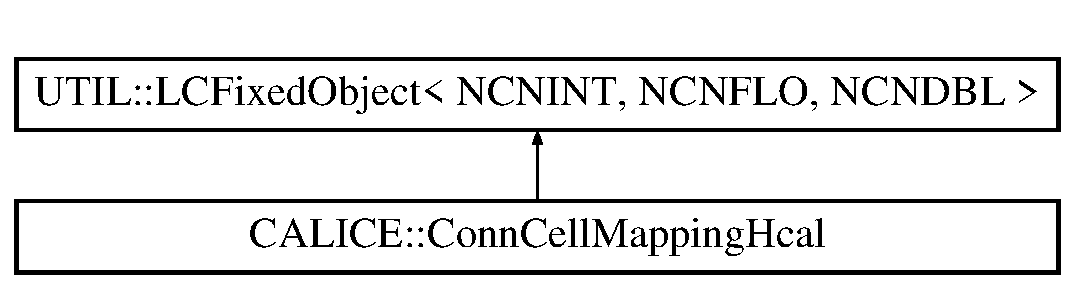
\includegraphics[height=2.000000cm]{classCALICE_1_1ConnCellMappingHcal}
\end{center}
\end{figure}
\subsection*{Public Member Functions}
\begin{DoxyCompactItemize}
\item 
{\bf Conn\-Cell\-Mapping\-Hcal} (int connpin, int icd\-\_\-fine, int jcd\-\_\-fine, int kcd\-\_\-fine, int icd\-\_\-coarse, int jcd\-\_\-coarse, int kcd\-\_\-coarse)\label{classCALICE_1_1ConnCellMappingHcal_ab42f668b5748b8dfa9b3fc97fa6c7fee}

\begin{DoxyCompactList}\small\item\em Convenient c'tor. \end{DoxyCompactList}\item 
{\bf Conn\-Cell\-Mapping\-Hcal} (L\-C\-Object $\ast$obj)\label{classCALICE_1_1ConnCellMappingHcal_a081e0f8e841d6f434e17b670cab48d7e}

\begin{DoxyCompactList}\small\item\em 'Copy constructor' needed to interpret L\-C\-Collection read from file/database. \end{DoxyCompactList}\item 
virtual {\bf $\sim$\-Conn\-Cell\-Mapping\-Hcal} ()\label{classCALICE_1_1ConnCellMappingHcal_a7a197aeb49859189e104e3d5d94d0391}

\begin{DoxyCompactList}\small\item\em Important for memory handling. \end{DoxyCompactList}\item 
int {\bf get\-Connpin} ()\label{classCALICE_1_1ConnCellMappingHcal_a98cddfbd965baa2a65f830c4b19c9dfc}

\begin{DoxyCompactList}\small\item\em the class interface\-: \end{DoxyCompactList}\item 
int {\bfseries get\-Cell\-I\-D\-\_\-fine} ()\label{classCALICE_1_1ConnCellMappingHcal_a86446b579f23ddac044afa98f83be109}

\item 
int {\bfseries get\-Cell\-I\-D\-\_\-coarse} ()\label{classCALICE_1_1ConnCellMappingHcal_a8136c2a1622f865fcdab81cda25284e5}

\item 
short {\bf get\-Cell\-Index\-\_\-fine} (std\-::string)\label{classCALICE_1_1ConnCellMappingHcal_acede8240bf218adff8d40e23d7c7903a}

\begin{DoxyCompactList}\small\item\em convenient getter functions \end{DoxyCompactList}\item 
short {\bfseries get\-Cell\-Index\-\_\-coarse} (std\-::string)\label{classCALICE_1_1ConnCellMappingHcal_aeb22fd5dbacc508100ff4b34d8d6d5e4}

\item 
void {\bfseries print} (std\-::ostream \&os)\label{classCALICE_1_1ConnCellMappingHcal_ad40f3d45f299b067ba913d53651c9102}

\item 
const std\-::string {\bf get\-Type\-Name} () const \label{classCALICE_1_1ConnCellMappingHcal_a824a0896a35021b8ea42da52c9bfae38}

\begin{DoxyCompactList}\small\item\em Type definition. \end{DoxyCompactList}\item 
const std\-::string {\bfseries get\-Data\-Description} () const \label{classCALICE_1_1ConnCellMappingHcal_a826f2d60b31e3329b5a68dccd014244f}

\end{DoxyCompactItemize}
\subsection*{Private Attributes}
\begin{DoxyCompactItemize}
\item 
short {\bf \-\_\-index}\label{classCALICE_1_1ConnCellMappingHcal_a63ebe04fafeb25e26b642d38b768cd71}

\begin{DoxyCompactList}\small\item\em i,j or k Index of the cell id \end{DoxyCompactList}\end{DoxyCompactItemize}


\subsection{Detailed Description}
Mapping class based on the L\-C\-Fixed\-Object template. 

that relates the mapping of the hcal connectors to the cellids 

Definition at line 33 of file Conn\-Cell\-Mapping\-Hcal.\-hh.



The documentation for this class was generated from the following files\-:\begin{DoxyCompactItemize}
\item 
Conn\-Cell\-Mapping\-Hcal.\-hh\item 
Conn\-Cell\-Mapping\-Hcal.\-cc\end{DoxyCompactItemize}

\section{C\-A\-L\-I\-C\-E\-:\-:Trigger\-Handler\-Calice\-:\-:Crate\-\_\-t Class Reference}
\label{classCALICE_1_1TriggerHandlerCalice_1_1Crate__t}\index{C\-A\-L\-I\-C\-E\-::\-Trigger\-Handler\-Calice\-::\-Crate\-\_\-t@{C\-A\-L\-I\-C\-E\-::\-Trigger\-Handler\-Calice\-::\-Crate\-\_\-t}}


Samll helper class which contains a collection of slots and which remebers all the sub detector ids conencted to it.  


\subsection*{Public Member Functions}
\begin{DoxyCompactItemize}
\item 
{\bfseries Crate\-\_\-t} (unsigned int sub\-\_\-det\-\_\-i)\label{classCALICE_1_1TriggerHandlerCalice_1_1Crate__t_a42dd3d017eb1e0981e92f1e57f3605c3}

\item 
bool {\bf is\-Used} () const \label{classCALICE_1_1TriggerHandlerCalice_1_1Crate__t_ab0daf2d8f75bf475fb0523c860e6aed1}

\begin{DoxyCompactList}\small\item\em Return true if this crate is connected to at least on known detector. \end{DoxyCompactList}\item 
bool {\bf is\-Used\-By\-Multiple\-Sub\-Detectors} () const \label{classCALICE_1_1TriggerHandlerCalice_1_1Crate__t_a3141c360228a0a289e147c4a285bb42e}

\begin{DoxyCompactList}\small\item\em Return true if the crate is connected to only one sub detector. \end{DoxyCompactList}\item 
void {\bf set\-Sub\-Detector\-I\-D} (unsigned int a\-\_\-sub\-\_\-dector)
\begin{DoxyCompactList}\small\item\em Return the I\-D of the sub detector which is connected to this crate. \end{DoxyCompactList}\item 
bool {\bf is\-Connected\-To\-Sub\-Detector} (unsigned int a\-\_\-sub\-\_\-dector) const \label{classCALICE_1_1TriggerHandlerCalice_1_1Crate__t_a00386bdf45d49e71cd8604393b5abc6a}

\begin{DoxyCompactList}\small\item\em Return true if the crate is conencted to the sub detector. \end{DoxyCompactList}\item 
{\bf Slot\-List\-\_\-t} \& {\bf slot\-List} ()\label{classCALICE_1_1TriggerHandlerCalice_1_1Crate__t_ab71658dc613ae2c3d5f683d643838567}

\begin{DoxyCompactList}\small\item\em Get the slotlist for read/write access. \end{DoxyCompactList}\item 
const {\bf Slot\-List\-\_\-t} \& {\bf slot\-List} () const \label{classCALICE_1_1TriggerHandlerCalice_1_1Crate__t_a9bd990db0cf9d53c6946e697faabd6f7}

\begin{DoxyCompactList}\small\item\em Get the slotlist for read only access. \end{DoxyCompactList}\end{DoxyCompactItemize}
\subsection*{Private Attributes}
\begin{DoxyCompactItemize}
\item 
std\-::vector$<$ unsigned int $>$ {\bfseries \-\_\-sub\-Det\-I\-D}\label{classCALICE_1_1TriggerHandlerCalice_1_1Crate__t_a49e7c92525f987ffb4b8b83446935ce1}

\item 
bool {\bfseries \-\_\-one\-Detector\-Only}\label{classCALICE_1_1TriggerHandlerCalice_1_1Crate__t_af6fa23743ffea3d191ab389b996cd6b7}

\item 
{\bf Slot\-List\-\_\-t} {\bfseries \-\_\-slots}\label{classCALICE_1_1TriggerHandlerCalice_1_1Crate__t_af7e308e0893ec31e1d83d54e5856371b}

\end{DoxyCompactItemize}


\subsection{Detailed Description}
Samll helper class which contains a collection of slots and which remebers all the sub detector ids conencted to it. 

Definition at line 569 of file Trigger\-Handler\-Calice.\-hh.



\subsection{Member Function Documentation}
\index{C\-A\-L\-I\-C\-E\-::\-Trigger\-Handler\-Calice\-::\-Crate\-\_\-t@{C\-A\-L\-I\-C\-E\-::\-Trigger\-Handler\-Calice\-::\-Crate\-\_\-t}!set\-Sub\-Detector\-I\-D@{set\-Sub\-Detector\-I\-D}}
\index{set\-Sub\-Detector\-I\-D@{set\-Sub\-Detector\-I\-D}!CALICE::TriggerHandlerCalice::Crate_t@{C\-A\-L\-I\-C\-E\-::\-Trigger\-Handler\-Calice\-::\-Crate\-\_\-t}}
\subsubsection[{set\-Sub\-Detector\-I\-D}]{\setlength{\rightskip}{0pt plus 5cm}void C\-A\-L\-I\-C\-E\-::\-Trigger\-Handler\-Calice\-::\-Crate\-\_\-t\-::set\-Sub\-Detector\-I\-D (
\begin{DoxyParamCaption}
\item[{unsigned int}]{a\-\_\-sub\-\_\-dector}
\end{DoxyParamCaption}
)\hspace{0.3cm}{\ttfamily [inline]}}\label{classCALICE_1_1TriggerHandlerCalice_1_1Crate__t_a4ad877cf64ba3e78b93d86d21834f281}


Return the I\-D of the sub detector which is connected to this crate. 

\begin{DoxySeeAlso}{See Also}
set 
\end{DoxySeeAlso}


Definition at line 588 of file Trigger\-Handler\-Calice.\-hh.



Referenced by C\-A\-L\-I\-C\-E\-::\-Trigger\-Handler\-Calice\-::module\-Connection\-Change().



The documentation for this class was generated from the following file\-:\begin{DoxyCompactItemize}
\item 
Trigger\-Handler\-Calice.\-hh\end{DoxyCompactItemize}

\section{C\-A\-L\-I\-C\-E\-:\-:D\-A\-Qconnection Class Reference}
\label{classCALICE_1_1DAQconnection}\index{C\-A\-L\-I\-C\-E\-::\-D\-A\-Qconnection@{C\-A\-L\-I\-C\-E\-::\-D\-A\-Qconnection}}


Class to store the D\-A\-Q address of a singel channel.  




{\ttfamily \#include $<$D\-A\-Qconnection.\-hh$>$}

Inheritance diagram for C\-A\-L\-I\-C\-E\-:\-:D\-A\-Qconnection\-:\begin{figure}[H]
\begin{center}
\leavevmode
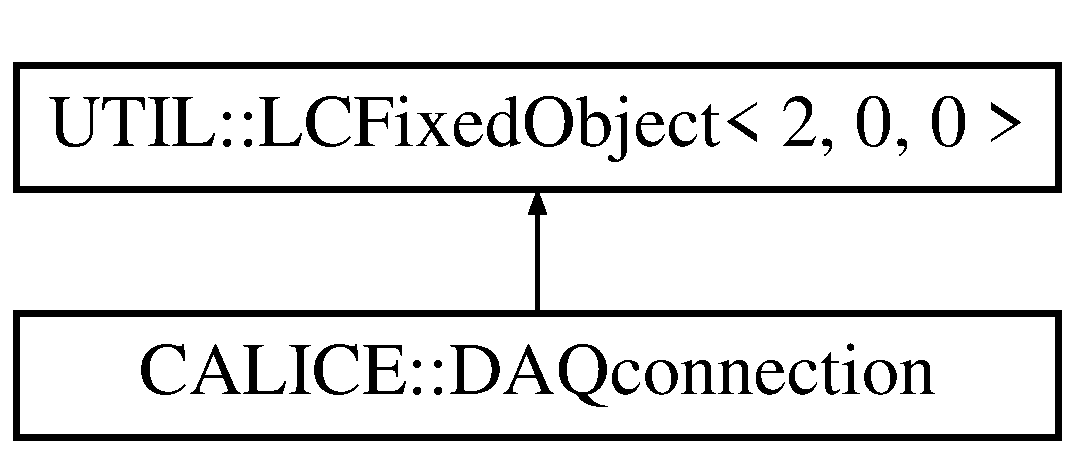
\includegraphics[height=2.000000cm]{classCALICE_1_1DAQconnection}
\end{center}
\end{figure}
\subsection*{Public Member Functions}
\begin{DoxyCompactItemize}
\item 
{\bf D\-A\-Qconnection} (const unsigned int crate, const unsigned slot, const unsigned int fe, const unsigned int chip, const unsigned int channel, const std\-::string enc=default\-Encoding\-String)\label{classCALICE_1_1DAQconnection_a1683f388c10013e8c435262de9c2b0a7}

\begin{DoxyCompactList}\small\item\em Constructor with initial values. \end{DoxyCompactList}\item 
{\bf D\-A\-Qconnection} (E\-V\-E\-N\-T\-::\-L\-C\-Object $\ast$object, const std\-::string enc=default\-Encoding\-String)\label{classCALICE_1_1DAQconnection_a7f6a1f3e76fe54b0f952cccf01b2b489}

\begin{DoxyCompactList}\small\item\em Constructor from L\-C\-Object. \end{DoxyCompactList}\item 
{\bf $\sim$\-D\-A\-Qconnection} ()\label{classCALICE_1_1DAQconnection_aab804c279b14b7139378825152f5d7af}

\begin{DoxyCompactList}\small\item\em Destructor. \end{DoxyCompactList}\item 
void {\bfseries set\-Channel} (unsigned int channel)\label{classCALICE_1_1DAQconnection_abc3d2a36439898873d04493ade4e2b79}

\item 
void {\bfseries set\-Chip} (unsigned int chip)\label{classCALICE_1_1DAQconnection_aa8749c6e343d3703cfd036a8a19851c8}

\item 
void {\bfseries set\-Fe} (unsigned int fe)\label{classCALICE_1_1DAQconnection_abbdb39c30e0d4c1709dc016fabbefabf}

\item 
void {\bfseries set\-Slot} (unsigned int slot)\label{classCALICE_1_1DAQconnection_a63a06aa5dda5881a3f19135cd5e42bf5}

\item 
void {\bfseries set\-Crate} (unsigned int crate)\label{classCALICE_1_1DAQconnection_aab13f456fa1e0f793b09820c82d9ada9}

\item 
unsigned int {\bfseries get\-Channel} () const \label{classCALICE_1_1DAQconnection_a5578725f9868a3c581425eca90fdd223}

\item 
unsigned int {\bfseries get\-Chip} () const \label{classCALICE_1_1DAQconnection_a4a783e2a4d37608d087479dc255731d2}

\item 
unsigned int {\bfseries get\-Fe} () const \label{classCALICE_1_1DAQconnection_ace1feda8e13487780aff0666eaadc83c}

\item 
unsigned int {\bfseries get\-Slot} () const \label{classCALICE_1_1DAQconnection_af873791c5318dc6496f96c16d1b782a7}

\item 
unsigned int {\bfseries get\-Crate} () const \label{classCALICE_1_1DAQconnection_a6379ea8cfc3e76ab748acae97e25553b}

\item 
const std\-::string {\bfseries get\-Encoding\-String} () const \label{classCALICE_1_1DAQconnection_aa1ccbcccb16b3ff6ace4b0e31c1d87ff}

\item 
const std\-::string {\bf get\-Type\-Name} () const \label{classCALICE_1_1DAQconnection_a25b1407516b5afd73f813662de211d7e}

\begin{DoxyCompactList}\small\item\em Implementation of L\-C\-Generic\-Object\-::get\-Type\-Name. \end{DoxyCompactList}\item 
const std\-::string {\bf get\-Data\-Description} () const \label{classCALICE_1_1DAQconnection_a7b2b9484febf8612c71291028c6675f4}

\begin{DoxyCompactList}\small\item\em Implementation of L\-C\-Generic\-Object\-::get\-Data\-Description. \end{DoxyCompactList}\end{DoxyCompactItemize}
\subsection*{Private Member Functions}
\begin{DoxyCompactItemize}
\item 
void {\bfseries update\-L\-Cobject} ()\label{classCALICE_1_1DAQconnection_a99cde9fbe145d08c6e60ce5946b28814}

\end{DoxyCompactItemize}
\subsection*{Private Attributes}
\begin{DoxyCompactItemize}
\item 
const std\-::string {\bfseries encoding\-String}\label{classCALICE_1_1DAQconnection_ae7c2fbe117b63706706a28ac96610975}

\item 
U\-T\-I\-L\-::\-Bit\-Field64 {\bfseries bit\-Field}\label{classCALICE_1_1DAQconnection_a6d3903a6b24a78eb1c73ec087aeb8df1}

\end{DoxyCompactItemize}


\subsection{Detailed Description}
Class to store the D\-A\-Q address of a singel channel. 

This class uses the mechanism of the Bit\-Field64 to encode and decode the bit positions using a string value. User defined encoding strings are possible. These have to define following fields\-: \begin{DoxyItemize}
\item crate The crate \item slot Slot in the crate \item fe Frontend on the card in slot \item chip Chip on the frontend \item channel Channel on the chip\end{DoxyItemize}
\begin{DoxyAuthor}{Author}
{\tt Benjamin.\-Lutz@desy.\-de} 
\end{DoxyAuthor}
\begin{DoxyVersion}{Version}
1.\-0 
\end{DoxyVersion}
\begin{DoxyDate}{Date}
September 2008 
\end{DoxyDate}


Definition at line 30 of file D\-A\-Qconnection.\-hh.



The documentation for this class was generated from the following files\-:\begin{DoxyCompactItemize}
\item 
D\-A\-Qconnection.\-hh\item 
D\-A\-Qconnection.\-cc\end{DoxyCompactItemize}

\section{C\-A\-L\-I\-C\-E\-:\-:Daq\-Run\-Summary\-Block Class Reference}
\label{classCALICE_1_1DaqRunSummaryBlock}\index{C\-A\-L\-I\-C\-E\-::\-Daq\-Run\-Summary\-Block@{C\-A\-L\-I\-C\-E\-::\-Daq\-Run\-Summary\-Block}}


Stores a summary of a run in terms of Number of Congfiuration Changes, Slow Readouts, Acquisitions and Number of Events in additions it stores the time of a run and for convenience the run number.  




{\ttfamily \#include $<$Daq\-Run\-Summary\-Block.\-hh$>$}

Inheritance diagram for C\-A\-L\-I\-C\-E\-:\-:Daq\-Run\-Summary\-Block\-:\begin{figure}[H]
\begin{center}
\leavevmode
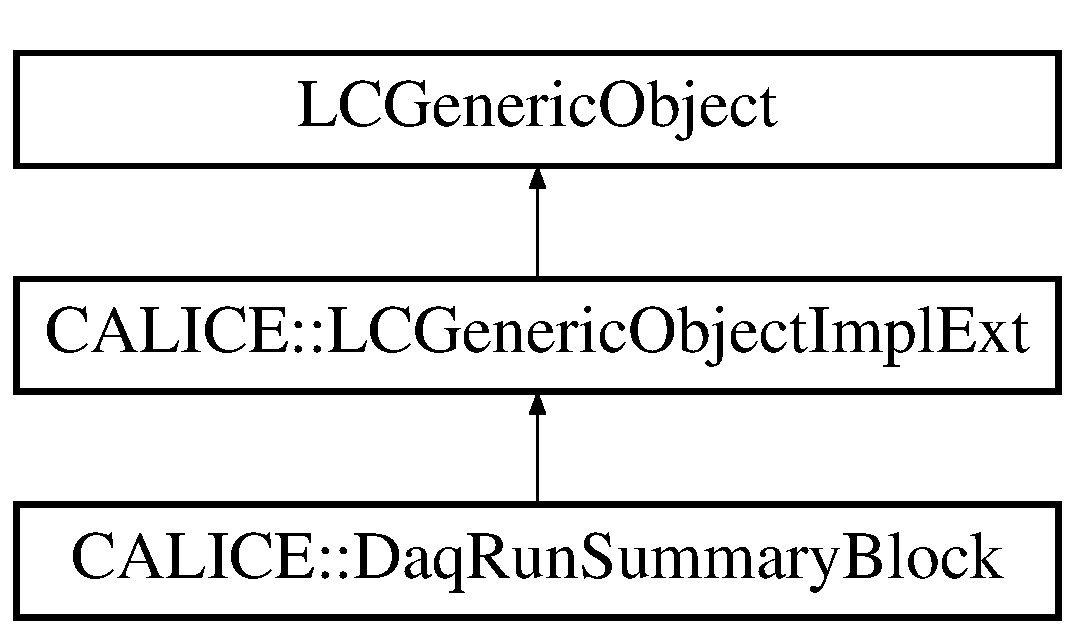
\includegraphics[height=3.000000cm]{classCALICE_1_1DaqRunSummaryBlock}
\end{center}
\end{figure}
\subsection*{Public Member Functions}
\begin{DoxyCompactItemize}
\item 
{\bf Daq\-Run\-Summary\-Block} ()\label{classCALICE_1_1DaqRunSummaryBlock_a6fd29ed6330baa493439cdc34e5a3448}

\begin{DoxyCompactList}\small\item\em Default Constructor. \end{DoxyCompactList}\item 
{\bf Daq\-Run\-Summary\-Block} (L\-C\-Object $\ast${\bf obj})\label{classCALICE_1_1DaqRunSummaryBlock_a70bdf0e2b5f667feaf48dd4340c2457c}

\begin{DoxyCompactList}\small\item\em 'Copy constructor' needed to interpret L\-C\-Collection read from file/database. \end{DoxyCompactList}\item 
{\bf Daq\-Run\-Summary\-Block} \& {\bf set\-Run\-Number} (int runnum)\label{classCALICE_1_1DaqRunSummaryBlock_ade14fb40860cd66831ea5401566c0404}

\begin{DoxyCompactList}\small\item\em Set the run number. \end{DoxyCompactList}\item 
int {\bf get\-Run\-Number} ()\label{classCALICE_1_1DaqRunSummaryBlock_afdf5fa9bb1dff6475117c66ea60aa103}

\begin{DoxyCompactList}\small\item\em Return the Number of Configurations. \end{DoxyCompactList}\item 
{\bf Daq\-Run\-Summary\-Block} \& {\bf set\-Number\-Of\-Configurations} (int numconf)\label{classCALICE_1_1DaqRunSummaryBlock_aaeb253c0f1165d200dd7bc540cac845a}

\begin{DoxyCompactList}\small\item\em Set the number of configurations. \end{DoxyCompactList}\item 
int {\bf get\-Number\-Of\-Configurations} ()\label{classCALICE_1_1DaqRunSummaryBlock_ac2bf2eb7f4d0d279cee5a36a690dca83}

\begin{DoxyCompactList}\small\item\em Return the Number of Configurations. \end{DoxyCompactList}\item 
{\bf Daq\-Run\-Summary\-Block} \& {\bf set\-Number\-Of\-Slow\-Readouts} (int numsro)\label{classCALICE_1_1DaqRunSummaryBlock_abed0d403b72287188068448c772b2885}

\begin{DoxyCompactList}\small\item\em Set the number of Slowreadouts. \end{DoxyCompactList}\item 
int {\bf get\-Number\-Of\-Slow\-Readouts} ()\label{classCALICE_1_1DaqRunSummaryBlock_a0452377daba7afe69a9a4c054f1034d0}

\begin{DoxyCompactList}\small\item\em Get the Number of Slowreadouts. \end{DoxyCompactList}\item 
{\bf Daq\-Run\-Summary\-Block} \& {\bf set\-Number\-Of\-Acquisitions} (int numacq)\label{classCALICE_1_1DaqRunSummaryBlock_a5224040c1df1bf17fc0c5ec5bd68f40f}

\begin{DoxyCompactList}\small\item\em Set the number of Acquisitions. \end{DoxyCompactList}\item 
int {\bf get\-Number\-Of\-Acquisitions} ()\label{classCALICE_1_1DaqRunSummaryBlock_acd32c04a0c561e223c71b4d96ba300da}

\begin{DoxyCompactList}\small\item\em Get the Number of Acquisitions. \end{DoxyCompactList}\item 
{\bf Daq\-Run\-Summary\-Block} \& {\bf set\-Number\-Of\-Events} (int numevt)\label{classCALICE_1_1DaqRunSummaryBlock_aee86dd895d3cf1fc0077581aebb5b28e}

\begin{DoxyCompactList}\small\item\em Set the number of Acquisitions. \end{DoxyCompactList}\item 
int {\bf get\-Number\-Of\-Events} ()\label{classCALICE_1_1DaqRunSummaryBlock_a8c025e9d7f400d419125f66fed82094e}

\begin{DoxyCompactList}\small\item\em Get the Number of Events. \end{DoxyCompactList}\item 
{\bf Daq\-Run\-Summary\-Block} \& {\bf set\-Run\-Duration} (int runtime)\label{classCALICE_1_1DaqRunSummaryBlock_a253c0fb4bdd59cac9285a89e94d2ba5f}

\begin{DoxyCompactList}\small\item\em Set the Run duration. \end{DoxyCompactList}\item 
int {\bf get\-Run\-Duration} ()\label{classCALICE_1_1DaqRunSummaryBlock_af63f5f6495d45bbc64c5e3b658d593fb}

\begin{DoxyCompactList}\small\item\em Get the Number of Events. \end{DoxyCompactList}\item 
void {\bf print} (std\-::ostream \&os)\label{classCALICE_1_1DaqRunSummaryBlock_a731d6d70fad2033515728de4bb6ba9eb}

\begin{DoxyCompactList}\small\item\em Convenient print method. \end{DoxyCompactList}\item 
const std\-::string {\bf get\-Type\-Name} () const \label{classCALICE_1_1DaqRunSummaryBlock_a001a655e6a0b1d141833bae6f4975234}

\begin{DoxyCompactList}\small\item\em Return the type of the class. \end{DoxyCompactList}\item 
const std\-::string {\bf get\-Data\-Description} () const \label{classCALICE_1_1DaqRunSummaryBlock_ac619c2fba39178ba2bb5180ddea1a369}

\begin{DoxyCompactList}\small\item\em Return a brief description of the data members. \end{DoxyCompactList}\end{DoxyCompactItemize}
\subsection*{Additional Inherited Members}


\subsection{Detailed Description}
Stores a summary of a run in terms of Number of Congfiuration Changes, Slow Readouts, Acquisitions and Number of Events in additions it stores the time of a run and for convenience the run number. 

\begin{DoxySeeAlso}{See Also}
\doxyref{Conditions\-Change\-Delegator}{p.}{classCALICE_1_1ConditionsChangeDelegator} 
\end{DoxySeeAlso}
\begin{DoxyAuthor}{Author}
R. Poeschl L\-A\-L (based on the other interface classes)
\end{DoxyAuthor}
\begin{DoxyDate}{Date}
Sep 2007 
\end{DoxyDate}


Definition at line 34 of file Daq\-Run\-Summary\-Block.\-hh.



The documentation for this class was generated from the following files\-:\begin{DoxyCompactItemize}
\item 
Daq\-Run\-Summary\-Block.\-hh\item 
Daq\-Run\-Summary\-Block.\-cc\end{DoxyCompactItemize}

\section{C\-A\-L\-I\-C\-E\-:\-:Daq\-Type\-Data\-Block Class Reference}
\label{classCALICE_1_1DaqTypeDataBlock}\index{C\-A\-L\-I\-C\-E\-::\-Daq\-Type\-Data\-Block@{C\-A\-L\-I\-C\-E\-::\-Daq\-Type\-Data\-Block}}


Base Class to handle all daq types (for the time being apart from the actual crc data) This base class constains the functions to store the data The actual handling of the data is left to dedicated classes which have to derive from this class.  




{\ttfamily \#include $<$Daq\-Type\-Data\-Block.\-hh$>$}

Inheritance diagram for C\-A\-L\-I\-C\-E\-:\-:Daq\-Type\-Data\-Block\-:\begin{figure}[H]
\begin{center}
\leavevmode
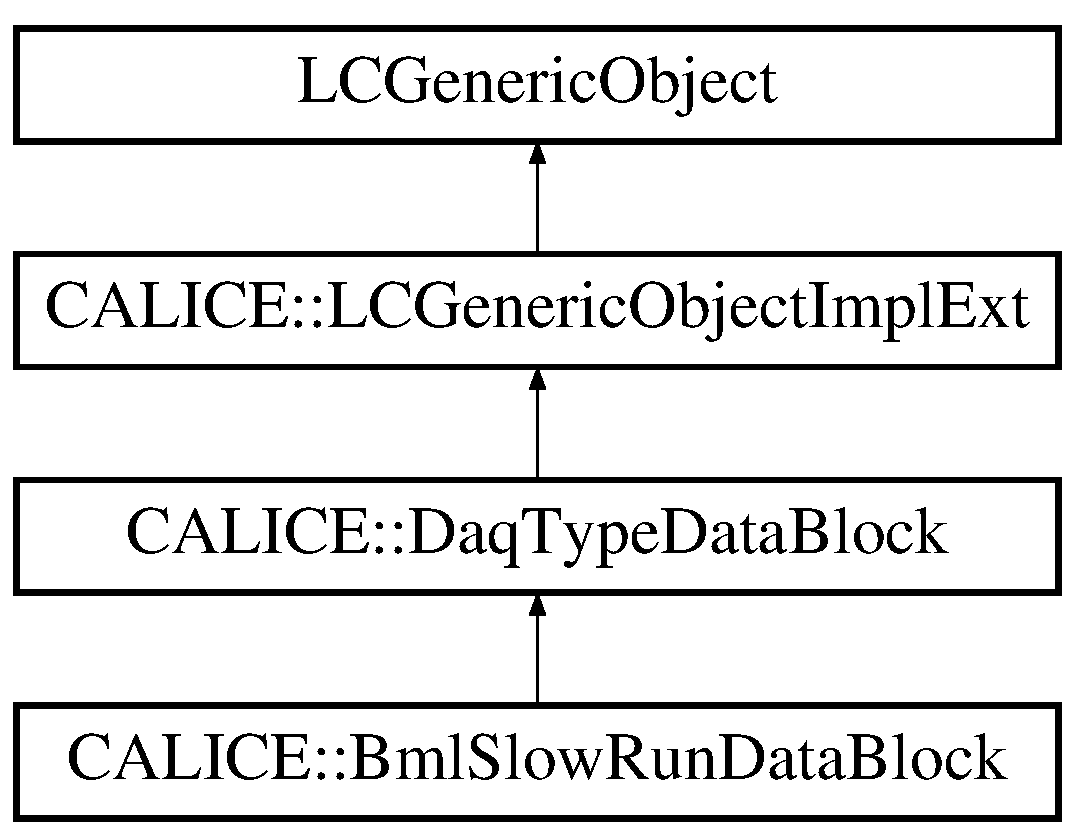
\includegraphics[height=4.000000cm]{classCALICE_1_1DaqTypeDataBlock}
\end{center}
\end{figure}
\subsection*{Public Member Functions}
\begin{DoxyCompactItemize}
\item 
{\bf Daq\-Type\-Data\-Block} ()\label{classCALICE_1_1DaqTypeDataBlock_a85c6645ef5c7c0806f3c3df59570f8cc}

\begin{DoxyCompactList}\small\item\em Constructor. \end{DoxyCompactList}\item 
{\bf Daq\-Type\-Data\-Block} (L\-C\-Object $\ast${\bf obj}, bool restore\-Maps=true)\label{classCALICE_1_1DaqTypeDataBlock_a1e706ee3c127aec373cef65488a6cb9f}

\begin{DoxyCompactList}\small\item\em 'Copy constructor' needed to interpret L\-C\-Collection read from file/database. \end{DoxyCompactList}\item 
{\bf Daq\-Type\-Data\-Block} \& {\bf set\-Time\-Stamps} (std\-::map$<$ std\-::string, time\-\_\-t $>$ time\-Stamp\-Map\-Raw)\label{classCALICE_1_1DaqTypeDataBlock_aa34e891e8a1fa5bf87f509d4b22cd385}

\begin{DoxyCompactList}\small\item\em Set the time stamps or better initialize the timestamp map which will be stored Remember\-: We store U\-T\-C!!!! \end{DoxyCompactList}\item 
{\bf Time\-Stamp\-Map\-\_\-t} {\bfseries get\-Time\-Stamps} ()\label{classCALICE_1_1DaqTypeDataBlock_a7d275918bef9692d3d514233587a6bf2}

\item 
virtual void {\bf set\-Dbl\-Arrays} (const {\bf Daq\-Type\-Data\-Dbl\-Map\-\_\-t} \&daq\-Type\-Data\-Dbl\-Map)\label{classCALICE_1_1DaqTypeDataBlock_a75a5676e055372817eb4ab644eac3d08}

\begin{DoxyCompactList}\small\item\em These methods receive the vectors with the measured values Mainly to store large arrays of a given datatype but in principle this can be extended to every entry in the interface class. \end{DoxyCompactList}\item 
virtual void {\bfseries set\-Float\-Arrays} (const Daq\-Type\-Data\-Float\-Map\-\_\-t \&daq\-Type\-Data\-Float\-Map)\label{classCALICE_1_1DaqTypeDataBlock_a012452bf9295a1cd73d0f7d8634b7253}

\item 
virtual void {\bfseries set\-Int\-Arrays} (const Daq\-Type\-Data\-U\-Int\-Map\-\_\-t \&)\label{classCALICE_1_1DaqTypeDataBlock_a98f2ff86e4ad4ba336a1e59ec0ceb34e}

\item 
virtual void {\bfseries set\-Int\-Arrays} (const Daq\-Type\-Data\-Int\-Map\-\_\-t \&)\label{classCALICE_1_1DaqTypeDataBlock_a134ce924a637904532cc22c1cc0f0ad1}

\item 
Daq\-Type\-Data\-Int\-Map\-\_\-t {\bf get\-Int\-Arrays} ()
\begin{DoxyCompactList}\small\item\em The following methods allow to retrieve the maps. \end{DoxyCompactList}\item 
{\bf Daq\-Type\-Data\-Dbl\-Map\-\_\-t} {\bfseries get\-Dbl\-Arrays} ()\label{classCALICE_1_1DaqTypeDataBlock_a971acc862569f0d3af2aa289b1cb4d5d}

\item 
Daq\-Type\-Data\-Float\-Map\-\_\-t {\bfseries get\-Float\-Arrays} ()\label{classCALICE_1_1DaqTypeDataBlock_a1c9066aad1370879f24f84464fd02da1}

\item 
{\bf Daq\-Type\-Data\-Block} $\ast$ {\bf finalize} ()
\begin{DoxyCompactList}\small\item\em A method which finally fills the object which is stored. \end{DoxyCompactList}\item 
virtual const double {\bf get\-Beam\-Energy} ()\label{classCALICE_1_1DaqTypeDataBlock_a22c56049653a7e3c0637deadb891e9da}

\begin{DoxyCompactList}\small\item\em A method to calculate the beam energy which has to be implemented by the derived classes. \end{DoxyCompactList}\item 
virtual void {\bf print} (std\-::ostream \&)\label{classCALICE_1_1DaqTypeDataBlock_a0ab5d656a67220cfc75fd842c29e1ac7}

\begin{DoxyCompactList}\small\item\em convenient print method \end{DoxyCompactList}\item 
const std\-::string {\bf get\-Type\-Name} () const \label{classCALICE_1_1DaqTypeDataBlock_acb717f063a4de474a5e51924f8d24682}

\begin{DoxyCompactList}\small\item\em Return the type of the class. \end{DoxyCompactList}\item 
const std\-::string {\bf get\-Data\-Description} () const \label{classCALICE_1_1DaqTypeDataBlock_a4dbed57cc9bf006bbd3e670f07fbe2b1}

\begin{DoxyCompactList}\small\item\em Return a brief description of the data members. \end{DoxyCompactList}\end{DoxyCompactItemize}
\subsection*{Private Member Functions}
\begin{DoxyCompactItemize}
\item 
void {\bf set\-Number\-Of\-Int\-Types} (int numvals)\label{classCALICE_1_1DaqTypeDataBlock_a28c2c09bb9a1ff30f199188a12ec7bab}

\begin{DoxyCompactList}\small\item\em Store the number of int data types. \end{DoxyCompactList}\item 
int {\bf get\-Number\-Of\-Int\-Types} () const \label{classCALICE_1_1DaqTypeDataBlock_adf260ba6c4d5c2178acda6bd6bf329b2}

\begin{DoxyCompactList}\small\item\em Retrieve the number of int data types. \end{DoxyCompactList}\item 
void {\bf set\-Number\-Of\-Time\-Stamps} (int numvals)\label{classCALICE_1_1DaqTypeDataBlock_a676aad32ad5a5634f384f236495f0ac9}

\begin{DoxyCompactList}\small\item\em Store the number of timestamps. \end{DoxyCompactList}\item 
int {\bf get\-Number\-Of\-Time\-Stamps} () const \label{classCALICE_1_1DaqTypeDataBlock_a6823cb2b2543bcebb87750ac5423e20e}

\begin{DoxyCompactList}\small\item\em Retrieve the number of int data types. \end{DoxyCompactList}\item 
void {\bf set\-Pointer\-To\-Index\-Of\-Int\-Type\-Names} (int nameind)\label{classCALICE_1_1DaqTypeDataBlock_ab5c75f5969f61b10ef90801babd1ab1f}

\begin{DoxyCompactList}\small\item\em Store the index at which the pointer to the names of the int data data types do start. \end{DoxyCompactList}\item 
int {\bf get\-Pointer\-To\-Index\-Of\-Int\-Type\-Names} () const \label{classCALICE_1_1DaqTypeDataBlock_a12176936fc593c6cb09bccc58dff9e25}

\begin{DoxyCompactList}\small\item\em Retrieve the index at which the pointer to the names of int data types do start. \end{DoxyCompactList}\item 
void {\bf set\-Pointer\-To\-Index\-Of\-Time\-Stamp\-Names} (int nameind)\label{classCALICE_1_1DaqTypeDataBlock_aac3f7e653792786bc85952f1ea97bba3}

\begin{DoxyCompactList}\small\item\em Store the index at which the pointer to the names of the time stamps do start. \end{DoxyCompactList}\item 
int {\bf get\-Pointer\-To\-Index\-Of\-Time\-Stamp\-Names} () const \label{classCALICE_1_1DaqTypeDataBlock_a52e2c8a7356f9b4fe5b0a190df3db19a}

\begin{DoxyCompactList}\small\item\em Retrieve the index at which the pointer to the names of the time stamps do start. \end{DoxyCompactList}\item 
void {\bf set\-Type\-Index} (int pos, int value)\label{classCALICE_1_1DaqTypeDataBlock_a622f0e34c6584942fc1d36c6ab038581}

\begin{DoxyCompactList}\small\item\em Set the index of a given data type name. \end{DoxyCompactList}\item 
void {\bf set\-Length\-Index\-Of\-Int\-Type\-Names} (int lengthindex)\label{classCALICE_1_1DaqTypeDataBlock_ab032d6110f9a55ef1f33db4d59197e84}

\begin{DoxyCompactList}\small\item\em Store the index at which the lengths of the names of the int data types do start. \end{DoxyCompactList}\item 
int {\bf get\-Length\-Index\-Of\-Int\-Type\-Names} () const \label{classCALICE_1_1DaqTypeDataBlock_a418917055bd74565de117b6c8ff50523}

\begin{DoxyCompactList}\small\item\em Retrieve the index at which the lengths of the names of the int data types do start. \end{DoxyCompactList}\item 
void {\bf set\-Length\-Index\-Of\-Time\-Stamp\-Names} (int lengthindex)\label{classCALICE_1_1DaqTypeDataBlock_afe7ffd23a9d39d2ce552f40227f0f8e6}

\begin{DoxyCompactList}\small\item\em Store the index at which the lengths of the names of the time stamps do start. \end{DoxyCompactList}\item 
int {\bf get\-Length\-Index\-Of\-Time\-Stamp\-Names} () const \label{classCALICE_1_1DaqTypeDataBlock_ae7a837206e4e801f31c5bd22fa0d1017}

\begin{DoxyCompactList}\small\item\em Retrieve the index at which the lengths of the names of the int data types do start. \end{DoxyCompactList}\item 
void {\bf set\-Size\-Index\-Of\-Int\-Type} (int size)\label{classCALICE_1_1DaqTypeDataBlock_a96726ed1f53f580959f9ae9f7eb579ca}

\begin{DoxyCompactList}\small\item\em Store the Index where the sizes of the int data data types do start. \end{DoxyCompactList}\item 
int {\bf get\-Size\-Index\-Of\-Int\-Type} () const \label{classCALICE_1_1DaqTypeDataBlock_a1f6e0831d20b7f3810ac080517ad7a49}

\begin{DoxyCompactList}\small\item\em Retrieve index where the sizes of int data types do start. \end{DoxyCompactList}\item 
void {\bf set\-Number\-Of\-Dbl\-Types} (int numvals)\label{classCALICE_1_1DaqTypeDataBlock_af22734d9ce54087e2c6b36832668da98}

\begin{DoxyCompactList}\small\item\em Store the number of double data types. \end{DoxyCompactList}\item 
int {\bf get\-Number\-Of\-Dbl\-Types} () const \label{classCALICE_1_1DaqTypeDataBlock_a4f409146da56fcddfbd2495149ea50cd}

\begin{DoxyCompactList}\small\item\em Retrieve the number of double data types. \end{DoxyCompactList}\item 
void {\bf set\-Pointer\-To\-Index\-Of\-Dbl\-Type\-Names} (int nameind)\label{classCALICE_1_1DaqTypeDataBlock_a8dbc1b40d1a11be5285a272ee01f597c}

\begin{DoxyCompactList}\small\item\em Store the at which the names the double data data types do start. \end{DoxyCompactList}\item 
int {\bf get\-Pointer\-To\-Index\-Of\-Dbl\-Type\-Names} () const \label{classCALICE_1_1DaqTypeDataBlock_a675b5c1436aeba8953a5c569889f1e84}

\begin{DoxyCompactList}\small\item\em Retrieve index at which the names of double data types do start. \end{DoxyCompactList}\item 
void {\bf set\-Length\-Index\-Of\-Dbl\-Type\-Names} (int length)\label{classCALICE_1_1DaqTypeDataBlock_ae8065e890645c324f6740947494fbe06}

\begin{DoxyCompactList}\small\item\em Store the index at which lengths of the names of the double data types do start. \end{DoxyCompactList}\item 
int {\bf get\-Length\-Index\-Of\-Dbl\-Type\-Names} () const \label{classCALICE_1_1DaqTypeDataBlock_ae302a22d40e2e009497ac8ffaaba1a47}

\begin{DoxyCompactList}\small\item\em Retrieve the index at which the lengths of the names of the double data types do start. \end{DoxyCompactList}\item 
void {\bf set\-Size\-Index\-Of\-Dbl\-Type} (int size)\label{classCALICE_1_1DaqTypeDataBlock_ad1c408aae59259c742b2aec8b3517b06}

\begin{DoxyCompactList}\small\item\em Store the Index where the sizes of the double data data types do start. \end{DoxyCompactList}\item 
int {\bf get\-Size\-Index\-Of\-Dbl\-Type} () const \label{classCALICE_1_1DaqTypeDataBlock_a84c98b620f0051e8aeadd93a6f2357b0}

\begin{DoxyCompactList}\small\item\em Retrieve index where the sizes of double data types do start. \end{DoxyCompactList}\item 
void {\bf set\-Number\-Of\-Float\-Types} (int numvals)\label{classCALICE_1_1DaqTypeDataBlock_a841cafcb827e3a396c0554c912240b15}

\begin{DoxyCompactList}\small\item\em Store the number of float data types. \end{DoxyCompactList}\item 
int {\bf get\-Number\-Of\-Float\-Types} () const \label{classCALICE_1_1DaqTypeDataBlock_a0e6f4e46a345d28c63d202d30b744a2e}

\begin{DoxyCompactList}\small\item\em Retrieve the number of float data types. \end{DoxyCompactList}\item 
void {\bf set\-Pointer\-To\-Index\-Of\-Float\-Type\-Names} (int nameind)\label{classCALICE_1_1DaqTypeDataBlock_a891466479bac0cbc2b7989808aa90865}

\begin{DoxyCompactList}\small\item\em Store the index at which the names of the float data types do start. \end{DoxyCompactList}\item 
int {\bf get\-Pointer\-To\-Index\-Of\-Float\-Type\-Names} () const \label{classCALICE_1_1DaqTypeDataBlock_a153fc0942be078682a9e4a83f4acf3e8}

\begin{DoxyCompactList}\small\item\em Retrieve index at which the names of the float data types do start. \end{DoxyCompactList}\item 
void {\bf set\-Length\-Index\-Of\-Float\-Type\-Names} (int length)\label{classCALICE_1_1DaqTypeDataBlock_a888df6e647e1a5e64a5bd38488315db1}

\begin{DoxyCompactList}\small\item\em Store the index at which the lengths of the names of the float data types do start. \end{DoxyCompactList}\item 
int {\bf get\-Length\-Index\-Of\-Float\-Type\-Names} () const \label{classCALICE_1_1DaqTypeDataBlock_acfc2ef22213129c57bacf00d1e27fa82}

\begin{DoxyCompactList}\small\item\em Retrieve the index at which the lengths of the names of the float data types do start. \end{DoxyCompactList}\item 
void {\bf set\-Size\-Index\-Of\-Float\-Type} (int size)\label{classCALICE_1_1DaqTypeDataBlock_acac139f2e46d4db6af0b6eddd6ec4942}

\begin{DoxyCompactList}\small\item\em Store the Index where the sizes of the float data data types do start. \end{DoxyCompactList}\item 
int {\bf get\-Size\-Index\-Of\-Float\-Type} () const \label{classCALICE_1_1DaqTypeDataBlock_ada9d6720bbd32244e611788b488d8d2a}

\begin{DoxyCompactList}\small\item\em Retrieve index where the sizes of double data types do start. \end{DoxyCompactList}\item 
void {\bf calculate\-Time\-Stamp} (struct tm $\ast$)\label{classCALICE_1_1DaqTypeDataBlock_a92c758b4cf990905756df438015a061d}

\begin{DoxyCompactList}\small\item\em Simple method to decompose the struct tm containing the timestamp into ints which can be stored in the L\-C\-Generic\-Object and therefore in the database. \end{DoxyCompactList}\item 
L\-C\-Time {\bf compose\-Time\-Stamp} ()\label{classCALICE_1_1DaqTypeDataBlock_a40444b0427fe536b7ea4bf14447a3df8}

\begin{DoxyCompactList}\small\item\em turn the two ints containing the timestamp info into a L\-C\-Time Object \end{DoxyCompactList}\item 
void {\bf Restore\-Maps} ()\label{classCALICE_1_1DaqTypeDataBlock_a57610189b303b049d13ef2b569e5156d}

\begin{DoxyCompactList}\small\item\em A method which restores the map from the generic object. \end{DoxyCompactList}\end{DoxyCompactItemize}
\subsection*{Private Attributes}
\begin{DoxyCompactItemize}
\item 
std\-::map$<$ std\-::string, time\-\_\-t $>$ {\bf \-\_\-time\-Stamp\-Map\-Raw}\label{classCALICE_1_1DaqTypeDataBlock_a8867f81834148bdf8a194e71b3b742f8}

\begin{DoxyCompactList}\small\item\em A map holds the nature and the value of the timestamps. \end{DoxyCompactList}\item 
{\bf Time\-Stamp\-Map\-\_\-t} {\bf \-\_\-time\-Stamp\-Map}\label{classCALICE_1_1DaqTypeDataBlock_aa4a278ab29ccecfee83baa22bdc993c0}

\begin{DoxyCompactList}\small\item\em Another map now with the time stamp using L\-C\-I\-O Utils. \end{DoxyCompactList}\item 
int {\bf \-\_\-timestamptoint} [2]\label{classCALICE_1_1DaqTypeDataBlock_a9ca2d41715983eb36a5fc1573d580a9c}

\begin{DoxyCompactList}\small\item\em A simple array which holds the timestamp decomposed into two ints containing a) ymd and b) hms. \end{DoxyCompactList}\item 
{\bf Daq\-Type\-Data\-Dbl\-Map\-\_\-t} {\bf \-\_\-buffer\-Of\-Dbls}\label{classCALICE_1_1DaqTypeDataBlock_a95a47d717cbc1a9988d43c37dcb92b43}

\begin{DoxyCompactList}\small\item\em Variables which buffer the maps passed by the converter Buffering is needed since we don't know a priori when the objects are passed to us and which data types they contain the 'finalize' method (see below) will finally create the object from the buffers Buffer for doubles. \end{DoxyCompactList}\item 
Daq\-Type\-Data\-Float\-Map\-\_\-t {\bf \-\_\-buffer\-Of\-Floats}\label{classCALICE_1_1DaqTypeDataBlock_a6bf50fbf5fe6cd66eecffd9e55ce482a}

\begin{DoxyCompactList}\small\item\em Buffer for Floats. \end{DoxyCompactList}\item 
Daq\-Type\-Data\-Int\-Map\-\_\-t {\bf \-\_\-buffer\-Of\-Ints}\label{classCALICE_1_1DaqTypeDataBlock_ab783f44996aab2ced5c9b2c88a183203}

\begin{DoxyCompactList}\small\item\em Buffer for Ints. \end{DoxyCompactList}\end{DoxyCompactItemize}
\subsection*{Additional Inherited Members}


\subsection{Detailed Description}
Base Class to handle all daq types (for the time being apart from the actual crc data) This base class constains the functions to store the data The actual handling of the data is left to dedicated classes which have to derive from this class. 

The implementation and the interpretation of the stored values is left to the derived classes. The actual meaning of the entries is propagated from a daq class into the database. Note, that in principle really all data types (apart from crc data) can be handled by this class However, existing interface classes (written before Oct. 2008) will remain untouched or exchanged gradually. if considered to be useful. This class allows for a quick reply to changes in the daq. In particular on the appearance of new data types. \begin{DoxyAuthor}{Author}
\-: Roman P�schl L\-A\-L/\-Orsay 
\end{DoxyAuthor}
\begin{DoxyDate}{Date}
Oct 2008 
\end{DoxyDate}


Definition at line 61 of file Daq\-Type\-Data\-Block.\-hh.



\subsection{Member Function Documentation}
\index{C\-A\-L\-I\-C\-E\-::\-Daq\-Type\-Data\-Block@{C\-A\-L\-I\-C\-E\-::\-Daq\-Type\-Data\-Block}!finalize@{finalize}}
\index{finalize@{finalize}!CALICE::DaqTypeDataBlock@{C\-A\-L\-I\-C\-E\-::\-Daq\-Type\-Data\-Block}}
\subsubsection[{finalize}]{\setlength{\rightskip}{0pt plus 5cm}{\bf Daq\-Type\-Data\-Block} $\ast$ C\-A\-L\-I\-C\-E\-::\-Daq\-Type\-Data\-Block\-::finalize (
\begin{DoxyParamCaption}
{}
\end{DoxyParamCaption}
)}\label{classCALICE_1_1DaqTypeDataBlock_a5aac4e6f4aef380287394ad36b30a40d}


A method which finally fills the object which is stored. 

\begin{DoxyRefDesc}{Todo}
\item[{\bf Todo}]can the algorithms in this method be templated? \end{DoxyRefDesc}


Definition at line 37 of file Daq\-Type\-Data\-Block.\-cc.



References \-\_\-buffer\-Of\-Dbls, \-\_\-buffer\-Of\-Floats, \-\_\-buffer\-Of\-Ints, \-\_\-time\-Stamp\-Map, \-\_\-time\-Stamp\-Map\-Raw, \-\_\-timestamptoint, calculate\-Time\-Stamp(), C\-A\-L\-I\-C\-E\-::convert\-String\-To\-Ints(), get\-Length\-Index\-Of\-Float\-Type\-Names(), get\-Number\-Of\-Dbl\-Types(), get\-Number\-Of\-Float\-Types(), get\-Number\-Of\-Int\-Types(), get\-Number\-Of\-Time\-Stamps(), get\-Pointer\-To\-Index\-Of\-Dbl\-Type\-Names(), get\-Pointer\-To\-Index\-Of\-Float\-Type\-Names(), get\-Pointer\-To\-Index\-Of\-Int\-Type\-Names(), get\-Pointer\-To\-Index\-Of\-Time\-Stamp\-Names(), C\-A\-L\-I\-C\-E\-::get\-String\-From\-Ints(), C\-A\-L\-I\-C\-E\-::\-L\-C\-Generic\-Object\-Impl\-Ext\-::obj(), Restore\-Maps(), set\-Length\-Index\-Of\-Dbl\-Type\-Names(), set\-Length\-Index\-Of\-Float\-Type\-Names(), set\-Length\-Index\-Of\-Int\-Type\-Names(), set\-Length\-Index\-Of\-Time\-Stamp\-Names(), set\-Number\-Of\-Dbl\-Types(), set\-Number\-Of\-Float\-Types(), set\-Number\-Of\-Int\-Types(), set\-Number\-Of\-Time\-Stamps(), set\-Pointer\-To\-Index\-Of\-Dbl\-Type\-Names(), set\-Pointer\-To\-Index\-Of\-Float\-Type\-Names(), set\-Pointer\-To\-Index\-Of\-Int\-Type\-Names(), set\-Pointer\-To\-Index\-Of\-Time\-Stamp\-Names(), set\-Size\-Index\-Of\-Dbl\-Type(), set\-Size\-Index\-Of\-Float\-Type(), set\-Size\-Index\-Of\-Int\-Type(), and set\-Type\-Index().

\index{C\-A\-L\-I\-C\-E\-::\-Daq\-Type\-Data\-Block@{C\-A\-L\-I\-C\-E\-::\-Daq\-Type\-Data\-Block}!get\-Int\-Arrays@{get\-Int\-Arrays}}
\index{get\-Int\-Arrays@{get\-Int\-Arrays}!CALICE::DaqTypeDataBlock@{C\-A\-L\-I\-C\-E\-::\-Daq\-Type\-Data\-Block}}
\subsubsection[{get\-Int\-Arrays}]{\setlength{\rightskip}{0pt plus 5cm}Daq\-Type\-Data\-Int\-Map\-\_\-t C\-A\-L\-I\-C\-E\-::\-Daq\-Type\-Data\-Block\-::get\-Int\-Arrays (
\begin{DoxyParamCaption}
{}
\end{DoxyParamCaption}
)\hspace{0.3cm}{\ttfamily [inline]}}\label{classCALICE_1_1DaqTypeDataBlock_aed8a8e75c1ca2befbf3f4c1bfe54e0a9}


The following methods allow to retrieve the maps. 

\begin{DoxyRefDesc}{Todo}
\item[{\bf Todo}]\-: Should these methods really be public or only accessible by friend functions or ...? 

\-: Do we have to check whether they has been filled or not before we hand it to the user? \end{DoxyRefDesc}


Definition at line 120 of file Daq\-Type\-Data\-Block.\-hh.



The documentation for this class was generated from the following files\-:\begin{DoxyCompactItemize}
\item 
Daq\-Type\-Data\-Block.\-hh\item 
Daq\-Type\-Data\-Block.\-cc\end{DoxyCompactItemize}

\section{C\-A\-L\-I\-C\-E\-:\-:Mapped\-Container$<$ T $>$\-:\-:Data\-With\-Address Class Reference}
\label{classCALICE_1_1MappedContainer_1_1DataWithAddress}\index{C\-A\-L\-I\-C\-E\-::\-Mapped\-Container$<$ T $>$\-::\-Data\-With\-Address@{C\-A\-L\-I\-C\-E\-::\-Mapped\-Container$<$ T $>$\-::\-Data\-With\-Address}}
\subsection*{Public Member Functions}
\begin{DoxyCompactItemize}
\item 
{\bfseries Data\-With\-Address} (const int address, T $\ast$data)\label{classCALICE_1_1MappedContainer_1_1DataWithAddress_ac7e3a4ba88ce83a52f8c8588e6e09f93}

\item 
int {\bfseries get\-Address} () const \label{classCALICE_1_1MappedContainer_1_1DataWithAddress_ad2f2af7218488e411b489579955b5abf}

\item 
T $\ast$ {\bfseries get\-Data} () const \label{classCALICE_1_1MappedContainer_1_1DataWithAddress_a9ac16b5083ddc5eb1768db68906583f5}

\end{DoxyCompactItemize}
\subsection*{Private Attributes}
\begin{DoxyCompactItemize}
\item 
int {\bfseries \-\_\-address}\label{classCALICE_1_1MappedContainer_1_1DataWithAddress_ab31d6a6ecdbf9cbbed05e7ba4d4204cc}

\item 
T $\ast$ {\bfseries \-\_\-data}\label{classCALICE_1_1MappedContainer_1_1DataWithAddress_a62a77e2b8874fd11ce0c8b065a4e369f}

\end{DoxyCompactItemize}


\subsection{Detailed Description}
\subsubsection*{template$<$class T$>$class C\-A\-L\-I\-C\-E\-::\-Mapped\-Container$<$ T $>$\-::\-Data\-With\-Address}



Definition at line 249 of file Mapped\-Container.\-hh.



The documentation for this class was generated from the following file\-:\begin{DoxyCompactItemize}
\item 
Mapped\-Container.\-hh\end{DoxyCompactItemize}

\section{C\-A\-L\-I\-C\-E\-:\-:D\-C\-Index Class Reference}
\label{classCALICE_1_1DCIndex}\index{C\-A\-L\-I\-C\-E\-::\-D\-C\-Index@{C\-A\-L\-I\-C\-E\-::\-D\-C\-Index}}
\subsection*{Public Member Functions}
\begin{DoxyCompactItemize}
\item 
{\bfseries D\-C\-Index} (const unsigned int, const unsigned int, const bool)\label{classCALICE_1_1DCIndex_ad63c29da71e51daf01b7fcd1b5406062}

\item 
const unsigned int {\bfseries D\-Clayer} () const \label{classCALICE_1_1DCIndex_aea8b6f0cca2779514d318bcbd1ef6b7e}

\item 
const unsigned int {\bfseries D\-Cxy} () const \label{classCALICE_1_1DCIndex_a513d6ebf343ab177f8d72ffa17e1fc3b}

\item 
const bool {\bfseries D\-Cnegative} () const \label{classCALICE_1_1DCIndex_a6b0d5449c8e6c7d707e12e4e5ef65c81}

\item 
{\bfseries D\-C\-Index} (const int)\label{classCALICE_1_1DCIndex_accc05b44244c93a41c9213d1e007c7e3}

\item 
const int {\bfseries index} () const \label{classCALICE_1_1DCIndex_a8133a5fb0d7ee839533f9130af9a16ed}

\end{DoxyCompactItemize}
\subsection*{Protected Member Functions}
\begin{DoxyCompactItemize}
\item 
void {\bfseries set} (const unsigned int, const unsigned int, const bool)\label{classCALICE_1_1DCIndex_a20505a45223c4772c74ff7b6969ba7b4}

\end{DoxyCompactItemize}
\subsection*{Private Attributes}
\begin{DoxyCompactItemize}
\item 
int {\bfseries \-\_\-index}\label{classCALICE_1_1DCIndex_af8b745008558ed0c6d90cdaba50da47f}

\end{DoxyCompactItemize}
\subsection*{Friends}
\begin{DoxyCompactItemize}
\item 
class {\bfseries Tdc\-Connection}\label{classCALICE_1_1DCIndex_ab85618aade64e98c6f7945f78e721566}

\end{DoxyCompactItemize}


\subsection{Detailed Description}


Definition at line 16 of file D\-C\-Index.\-hh.



The documentation for this class was generated from the following files\-:\begin{DoxyCompactItemize}
\item 
D\-C\-Index.\-hh\item 
D\-C\-Index.\-cc\end{DoxyCompactItemize}

\section{C\-A\-L\-I\-C\-E\-:\-:Dead\-Noise\-Constants Class Reference}
\label{classCALICE_1_1DeadNoiseConstants}\index{C\-A\-L\-I\-C\-E\-::\-Dead\-Noise\-Constants@{C\-A\-L\-I\-C\-E\-::\-Dead\-Noise\-Constants}}


Class to store the results of a selection of dead or noisy cells for a certain chip/channel for a fixed module\-I\-D.  




{\ttfamily \#include $<$Dead\-Noise\-Constants.\-hh$>$}

Inheritance diagram for C\-A\-L\-I\-C\-E\-:\-:Dead\-Noise\-Constants\-:\begin{figure}[H]
\begin{center}
\leavevmode
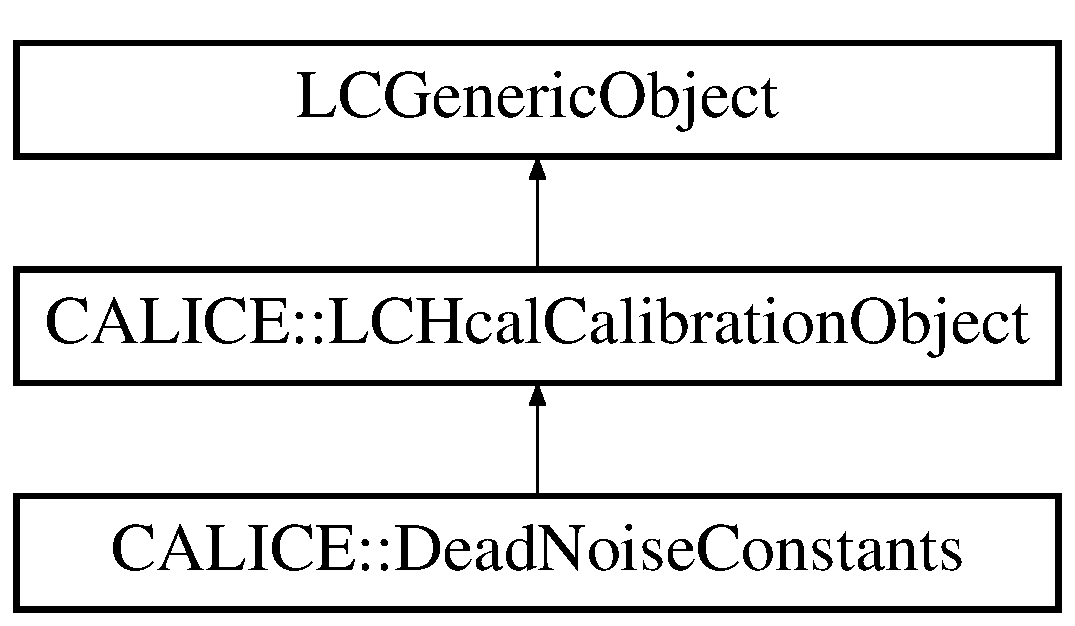
\includegraphics[height=3.000000cm]{classCALICE_1_1DeadNoiseConstants}
\end{center}
\end{figure}
\subsection*{Public Member Functions}
\begin{DoxyCompactItemize}
\item 
{\bf Dead\-Noise\-Constants} ()\label{classCALICE_1_1DeadNoiseConstants_a12212bb9fea94ac0480654f7115f77d7}

\begin{DoxyCompactList}\small\item\em default constructor \end{DoxyCompactList}\item 
{\bf Dead\-Noise\-Constants} (unsigned chip, unsigned channel, int dead\-Level, int noise\-Level)
\begin{DoxyCompactList}\small\item\em constructor, initializing with parameters \end{DoxyCompactList}\item 
{\bfseries Dead\-Noise\-Constants} (L\-C\-Object $\ast${\bf obj})\label{classCALICE_1_1DeadNoiseConstants_a8302f5e506b0cf1d98fc2bbb481e4b99}

\item 
int {\bf get\-Dead\-Level} () const \label{classCALICE_1_1DeadNoiseConstants_a10bc03bb0aa616f22eb1f1a734089858}

\begin{DoxyCompactList}\small\item\em get cell dead level \end{DoxyCompactList}\item 
float {\bf get\-Noise\-Level} () const \label{classCALICE_1_1DeadNoiseConstants_aea5232b89fb4db1f000539ac7b85e3e8}

\begin{DoxyCompactList}\small\item\em get cell noise level \end{DoxyCompactList}\item 
float {\bf apply\-Calibration} (float input\-Value) const 
\begin{DoxyCompactList}\small\item\em apply calibration to energy value \end{DoxyCompactList}\item 
float {\bf apply\-Calibration\-Error} (float input\-Value, float input\-Error) const 
\begin{DoxyCompactList}\small\item\em apply calibration error to current error \end{DoxyCompactList}\item 
bool {\bf calibration\-Valid} () const 
\begin{DoxyCompactList}\small\item\em check if a valid calibration is available \end{DoxyCompactList}\item 
bool {\bf keep\-Event} (float result\-Value, float result\-Error) const 
\begin{DoxyCompactList}\small\item\em accept only non-\/dead and non-\/noisy events \end{DoxyCompactList}\item 
void {\bf print} (std\-::ostream \&os)\label{classCALICE_1_1DeadNoiseConstants_a0c183f8c95da9581b250363ef26b2c21}

\begin{DoxyCompactList}\small\item\em convenient print method \end{DoxyCompactList}\item 
const std\-::string {\bf get\-Type\-Name} () const \label{classCALICE_1_1DeadNoiseConstants_a7560a94ebb09e6b925b2988fbeda12e0}

\begin{DoxyCompactList}\small\item\em return type of the class \end{DoxyCompactList}\item 
const std\-::string {\bf get\-Data\-Description} () const \label{classCALICE_1_1DeadNoiseConstants_a618908e466b60a838ecc6667971e6ad2}

\begin{DoxyCompactList}\small\item\em return a brief description of the data member \end{DoxyCompactList}\end{DoxyCompactItemize}
\subsection*{Additional Inherited Members}


\subsection{Detailed Description}
Class to store the results of a selection of dead or noisy cells for a certain chip/channel for a fixed module\-I\-D. 

\begin{DoxyAuthor}{Author}
S. Schmidt D\-E\-S\-Y 
\end{DoxyAuthor}
\begin{DoxyDate}{Date}
Sep 25 2006 
\end{DoxyDate}


Definition at line 25 of file Dead\-Noise\-Constants.\-hh.



\subsection{Constructor \& Destructor Documentation}
\index{C\-A\-L\-I\-C\-E\-::\-Dead\-Noise\-Constants@{C\-A\-L\-I\-C\-E\-::\-Dead\-Noise\-Constants}!Dead\-Noise\-Constants@{Dead\-Noise\-Constants}}
\index{Dead\-Noise\-Constants@{Dead\-Noise\-Constants}!CALICE::DeadNoiseConstants@{C\-A\-L\-I\-C\-E\-::\-Dead\-Noise\-Constants}}
\subsubsection[{Dead\-Noise\-Constants}]{\setlength{\rightskip}{0pt plus 5cm}C\-A\-L\-I\-C\-E\-::\-Dead\-Noise\-Constants\-::\-Dead\-Noise\-Constants (
\begin{DoxyParamCaption}
\item[{unsigned}]{chip, }
\item[{unsigned}]{channel, }
\item[{int}]{dead\-Level, }
\item[{int}]{noise\-Level}
\end{DoxyParamCaption}
)\hspace{0.3cm}{\ttfamily [inline]}}\label{classCALICE_1_1DeadNoiseConstants_a40bec0935780cdf617c71ca3f46af6a1}


constructor, initializing with parameters 


\begin{DoxyParams}{Parameters}
{\em chip} & chip number of cell to be calibrated \\
\hline
{\em channel} & channel number of cell to be calibrated \\
\hline
{\em dead\-Level} & \char`\"{}level\char`\"{} of being dead for a cell, 0\-: not dead, 1\-: dead \\
\hline
{\em noise\-Level} & \char`\"{}level\char`\"{} of being noisy for a cell, 0\-: no noise, 1\-: low noise, 2\-: high noise \\
\hline
\end{DoxyParams}


Definition at line 39 of file Dead\-Noise\-Constants.\-hh.



\subsection{Member Function Documentation}
\index{C\-A\-L\-I\-C\-E\-::\-Dead\-Noise\-Constants@{C\-A\-L\-I\-C\-E\-::\-Dead\-Noise\-Constants}!apply\-Calibration@{apply\-Calibration}}
\index{apply\-Calibration@{apply\-Calibration}!CALICE::DeadNoiseConstants@{C\-A\-L\-I\-C\-E\-::\-Dead\-Noise\-Constants}}
\subsubsection[{apply\-Calibration}]{\setlength{\rightskip}{0pt plus 5cm}float C\-A\-L\-I\-C\-E\-::\-Dead\-Noise\-Constants\-::apply\-Calibration (
\begin{DoxyParamCaption}
\item[{float}]{input\-Value}
\end{DoxyParamCaption}
) const\hspace{0.3cm}{\ttfamily [inline]}, {\ttfamily [virtual]}}\label{classCALICE_1_1DeadNoiseConstants_a117a93e472c84e57b805de35e12b6e29}


apply calibration to energy value 


\begin{DoxyParams}{Parameters}
{\em input\-Value} & \char`\"{}energy\char`\"{} value before the calibration \\
\hline
\end{DoxyParams}
\begin{DoxyReturn}{Returns}
as the selection of non-\/dead/non-\/noisy cells has no impact on the \char`\"{}energy\char`\"{} the input\-Value is returned 
\end{DoxyReturn}


Reimplemented from {\bf C\-A\-L\-I\-C\-E\-::\-L\-C\-Hcal\-Calibration\-Object} \doxyref{}{p.}{classCALICE_1_1LCHcalCalibrationObject_a763f1cf5b9c372fdde268d79b789adcc}.



Definition at line 67 of file Dead\-Noise\-Constants.\-hh.

\index{C\-A\-L\-I\-C\-E\-::\-Dead\-Noise\-Constants@{C\-A\-L\-I\-C\-E\-::\-Dead\-Noise\-Constants}!apply\-Calibration\-Error@{apply\-Calibration\-Error}}
\index{apply\-Calibration\-Error@{apply\-Calibration\-Error}!CALICE::DeadNoiseConstants@{C\-A\-L\-I\-C\-E\-::\-Dead\-Noise\-Constants}}
\subsubsection[{apply\-Calibration\-Error}]{\setlength{\rightskip}{0pt plus 5cm}float C\-A\-L\-I\-C\-E\-::\-Dead\-Noise\-Constants\-::apply\-Calibration\-Error (
\begin{DoxyParamCaption}
\item[{float}]{input\-Value, }
\item[{float}]{input\-Error}
\end{DoxyParamCaption}
) const\hspace{0.3cm}{\ttfamily [inline]}, {\ttfamily [virtual]}}\label{classCALICE_1_1DeadNoiseConstants_a1c5558e71e236dabf1e54f54a87162f0}


apply calibration error to current error 


\begin{DoxyParams}{Parameters}
{\em input\-Value} & \char`\"{}energy\char`\"{} value before the calibration \\
\hline
{\em input\-Error} & error of the \char`\"{}energy\char`\"{} value before the calibration \\
\hline
\end{DoxyParams}
\begin{DoxyReturn}{Returns}
as the selection of non-\/dead/non-\/noisy cells has no error the input\-Error is returned 
\end{DoxyReturn}


Reimplemented from {\bf C\-A\-L\-I\-C\-E\-::\-L\-C\-Hcal\-Calibration\-Object} \doxyref{}{p.}{classCALICE_1_1LCHcalCalibrationObject_a16d9de9567f68d7784a2daa4d2821341}.



Definition at line 76 of file Dead\-Noise\-Constants.\-hh.

\index{C\-A\-L\-I\-C\-E\-::\-Dead\-Noise\-Constants@{C\-A\-L\-I\-C\-E\-::\-Dead\-Noise\-Constants}!calibration\-Valid@{calibration\-Valid}}
\index{calibration\-Valid@{calibration\-Valid}!CALICE::DeadNoiseConstants@{C\-A\-L\-I\-C\-E\-::\-Dead\-Noise\-Constants}}
\subsubsection[{calibration\-Valid}]{\setlength{\rightskip}{0pt plus 5cm}bool C\-A\-L\-I\-C\-E\-::\-Dead\-Noise\-Constants\-::calibration\-Valid (
\begin{DoxyParamCaption}
{}
\end{DoxyParamCaption}
) const\hspace{0.3cm}{\ttfamily [inline]}, {\ttfamily [virtual]}}\label{classCALICE_1_1DeadNoiseConstants_ad7e3bc3298b47d8fa31a43c160a8a45b}


check if a valid calibration is available 

\begin{DoxyReturn}{Returns}
true as the selection of non-\/dead/non-\/noisy cells is always valid 
\end{DoxyReturn}


Reimplemented from {\bf C\-A\-L\-I\-C\-E\-::\-L\-C\-Hcal\-Calibration\-Object} \doxyref{}{p.}{classCALICE_1_1LCHcalCalibrationObject_abbb1fce81f41a89147b721d593bbc734}.



Definition at line 83 of file Dead\-Noise\-Constants.\-hh.

\index{C\-A\-L\-I\-C\-E\-::\-Dead\-Noise\-Constants@{C\-A\-L\-I\-C\-E\-::\-Dead\-Noise\-Constants}!keep\-Event@{keep\-Event}}
\index{keep\-Event@{keep\-Event}!CALICE::DeadNoiseConstants@{C\-A\-L\-I\-C\-E\-::\-Dead\-Noise\-Constants}}
\subsubsection[{keep\-Event}]{\setlength{\rightskip}{0pt plus 5cm}bool C\-A\-L\-I\-C\-E\-::\-Dead\-Noise\-Constants\-::keep\-Event (
\begin{DoxyParamCaption}
\item[{float}]{result\-Value, }
\item[{float}]{result\-Error}
\end{DoxyParamCaption}
) const\hspace{0.3cm}{\ttfamily [inline]}, {\ttfamily [virtual]}}\label{classCALICE_1_1DeadNoiseConstants_af4318e256ff1466682855553d5ba453e}


accept only non-\/dead and non-\/noisy events 


\begin{DoxyParams}{Parameters}
{\em result\-Value} & \char`\"{}energy\char`\"{} value after the calibration \\
\hline
{\em result\-Error} & error of the \char`\"{}energy\char`\"{} value after the calibration \\
\hline
\end{DoxyParams}
\begin{DoxyReturn}{Returns}
true if a cell is non-\/dead and non-\/noisy 
\end{DoxyReturn}


Reimplemented from {\bf C\-A\-L\-I\-C\-E\-::\-L\-C\-Hcal\-Calibration\-Object} \doxyref{}{p.}{classCALICE_1_1LCHcalCalibrationObject_a59f14a6b83e77717751ae4e7213e8d09}.



Definition at line 92 of file Dead\-Noise\-Constants.\-hh.



The documentation for this class was generated from the following files\-:\begin{DoxyCompactItemize}
\item 
Dead\-Noise\-Constants.\-hh\item 
Dead\-Noise\-Constants.\-cc\end{DoxyCompactItemize}

\section{C\-A\-L\-I\-C\-E\-:\-:Decoder\-Set Class Reference}
\label{classCALICE_1_1DecoderSet}\index{C\-A\-L\-I\-C\-E\-::\-Decoder\-Set@{C\-A\-L\-I\-C\-E\-::\-Decoder\-Set}}


class containing decoders for the three \doxyref{C\-A\-L\-I\-C\-E}{p.}{namespaceCALICE} coordinate systems  




{\ttfamily \#include $<$Decoder\-Set.\-hh$>$}

\subsection*{Data Structures}
\begin{DoxyCompactItemize}
\item 
struct {\bf Mokka\-I\-D\-\_\-t}
\end{DoxyCompactItemize}
\subsection*{Public Member Functions}
\begin{DoxyCompactItemize}
\item 
{\bf Decoder\-Set} ()
\begin{DoxyCompactList}\small\item\em standard constructor \end{DoxyCompactList}\item 
{\bf Decoder\-Set} (const std\-::string \&cell\-I\-Dencoding, const std\-::string \&module\-Encoding, const std\-::string \&D\-A\-Qencoding)
\begin{DoxyCompactList}\small\item\em constructor with encoding strings \end{DoxyCompactList}\item 
void {\bf set\-Cell\-I\-D\-Encoding} (const std\-::string \&encoding)
\begin{DoxyCompactList}\small\item\em set a new cell I\-D encoding string if an empty string is given the function will use the default encoding string \end{DoxyCompactList}\item 
void {\bf set\-Module\-Encoding} (const std\-::string \&encoding)
\begin{DoxyCompactList}\small\item\em set a new Module tile encoding string if an empty string is given the function will use the default encoding string \end{DoxyCompactList}\item 
void {\bf set\-D\-A\-Q\-Encoding} (const std\-::string \&encoding)
\begin{DoxyCompactList}\small\item\em set a new D\-A\-Q channel I\-D encoding string if an empty string is given the function will use the default encoding string \end{DoxyCompactList}\item 
const std\-::string \& {\bf get\-Cell\-I\-D\-Encoding} () const 
\begin{DoxyCompactList}\small\item\em get the current cell I\-D encoding string \end{DoxyCompactList}\item 
const std\-::string \& {\bf get\-Module\-Encoding} () const 
\begin{DoxyCompactList}\small\item\em get the current Module tile encoding string \end{DoxyCompactList}\item 
const std\-::string \& {\bf get\-D\-A\-Q\-Encoding} () const 
\begin{DoxyCompactList}\small\item\em get the current D\-A\-Q channel I\-D encoding string \end{DoxyCompactList}\item 
unsigned int {\bf get\-I\-From\-Cell\-I\-D} (const int cell\-I\-D) const 
\begin{DoxyCompactList}\small\item\em get I from (Mokka) Cell\-I\-D The right encoding string has to be set before. \end{DoxyCompactList}\item 
unsigned int {\bf get\-J\-From\-Cell\-I\-D} (const int cell\-I\-D) const 
\begin{DoxyCompactList}\small\item\em get J from (Mokka) Cell\-I\-D The right encoding string has to be set before. \end{DoxyCompactList}\item 
unsigned int {\bf get\-K\-From\-Cell\-I\-D} (const int cell\-I\-D) const 
\begin{DoxyCompactList}\small\item\em get K from (Mokka) Cell\-I\-D The right encoding string has to be set before. \end{DoxyCompactList}\item 
unsigned int {\bf get\-Module\-From\-Module\-I\-D} (const int module\-I\-D) const 
\begin{DoxyCompactList}\small\item\em get module from (Module) channel I\-D The right encoding string has to be set before. \end{DoxyCompactList}\item 
unsigned int {\bf get\-Chip\-From\-Module\-I\-D} (const int module\-I\-D) const 
\begin{DoxyCompactList}\small\item\em get chip from (Module) channel I\-D The right encoding string has to be set before. \end{DoxyCompactList}\item 
unsigned int {\bf get\-Channel\-From\-Module\-I\-D} (const int module\-I\-D) const 
\begin{DoxyCompactList}\small\item\em get channel from (Module) channel I\-D The right encoding string has to be set before. \end{DoxyCompactList}\item 
unsigned int {\bf get\-Channel\-From\-D\-A\-Q\-I\-D} (const int {\bf D\-A\-Qconnection}) const 
\begin{DoxyCompactList}\small\item\em get channel from D\-A\-Q channel I\-D The right encoding string has to be set before. \end{DoxyCompactList}\item 
unsigned int {\bf get\-Chip\-From\-D\-A\-Q\-I\-D} (const int {\bf D\-A\-Qconnection}) const 
\begin{DoxyCompactList}\small\item\em get chip from D\-A\-Q channel I\-D The right encoding string has to be set before. \end{DoxyCompactList}\item 
unsigned int {\bf get\-Fe\-From\-D\-A\-Q\-I\-D} (const int {\bf D\-A\-Qconnection}) const 
\begin{DoxyCompactList}\small\item\em get fe from D\-A\-Q channel I\-D The right encoding string has to be set before. \end{DoxyCompactList}\item 
unsigned int {\bf get\-Slot\-From\-D\-A\-Q\-I\-D} (const int {\bf D\-A\-Qconnection}) const 
\begin{DoxyCompactList}\small\item\em get slot from D\-A\-Q channel I\-D The right encoding string has to be set before. \end{DoxyCompactList}\item 
unsigned int {\bf get\-Crate\-From\-D\-A\-Q\-I\-D} (const int {\bf D\-A\-Qconnection}) const 
\begin{DoxyCompactList}\small\item\em get crate from D\-A\-Q channel I\-D The right encoding string has to be set before. \end{DoxyCompactList}\item 
int {\bf get\-Cell\-I\-D} (const unsigned int I, const unsigned int J, const unsigned int K) const 
\begin{DoxyCompactList}\small\item\em get Cell\-I\-D from triple I,J,K \end{DoxyCompactList}\item 
int {\bf get\-Module\-I\-D} (const unsigned int module, const unsigned int chip, const unsigned int channel) const 
\begin{DoxyCompactList}\small\item\em get (Module) channel I\-D from triple module, chip, channel \end{DoxyCompactList}\item 
int {\bf get\-D\-A\-Q\-I\-D} (const unsigned int crate, const unsigned int slot, const unsigned int fe, const unsigned int chip, const unsigned int channel) const 
\begin{DoxyCompactList}\small\item\em get D\-A\-Q channel I\-D from crate, slot, fe, chip, channel \end{DoxyCompactList}\end{DoxyCompactItemize}
\subsection*{Private Types}
\begin{DoxyCompactItemize}
\item 
typedef std\-::map$<$ std\-::string, \\*
{\bf Mokka\-I\-D\-\_\-t} $>$ {\bfseries mokka\-Decoder\-Map\-\_\-t}\label{classCALICE_1_1DecoderSet_aaa60db49451c3183f3b44c7738a3eb2e}

\end{DoxyCompactItemize}
\subsection*{Private Attributes}
\begin{DoxyCompactItemize}
\item 
std\-::string {\bfseries \-\_\-cell\-I\-Dencoding\-String}\label{classCALICE_1_1DecoderSet_adabb4fa6971abdefb51e793dbd4afc80}

\item 
std\-::string {\bfseries \-\_\-module\-I\-D\-Encoding\-String}\label{classCALICE_1_1DecoderSet_a00fe23b51254c77dbc495dcec6075447}

\item 
std\-::string {\bfseries \-\_\-daq\-I\-Dencoding\-String}\label{classCALICE_1_1DecoderSet_a1b8a88e2732336e6ac7a80acdf7d6f62}

\item 
{\bf Fast\-Decoder} $\ast$ {\bfseries \-\_\-\-I\-From\-Cell\-I\-D}\label{classCALICE_1_1DecoderSet_af543cade302a4724ddba67b313c39f76}

\item 
{\bf Fast\-Decoder} $\ast$ {\bfseries \-\_\-\-J\-From\-Cell\-I\-D}\label{classCALICE_1_1DecoderSet_a5c6c387c762f0e425e7477ee9cbb759e}

\item 
{\bf Fast\-Decoder} $\ast$ {\bfseries \-\_\-\-K\-From\-Cell\-I\-D}\label{classCALICE_1_1DecoderSet_acc617bd3d0f5ea5de5634c552d6c0d7c}

\item 
{\bf Fast\-Decoder} $\ast$ {\bfseries \-\_\-module\-From\-Module\-I\-D}\label{classCALICE_1_1DecoderSet_a480f62a678cdd42278f315455607a8dd}

\item 
{\bf Fast\-Decoder} $\ast$ {\bfseries \-\_\-chip\-From\-Module\-I\-D}\label{classCALICE_1_1DecoderSet_a8c22d248c09b54673a5333da4c410047}

\item 
{\bf Fast\-Decoder} $\ast$ {\bfseries \-\_\-channel\-From\-Module\-I\-D}\label{classCALICE_1_1DecoderSet_a5f7a75f6f5e1c663a9791c0bee9588a4}

\item 
{\bf Fast\-Decoder} $\ast$ {\bfseries \-\_\-channel\-From\-D\-A\-Q\-I\-D}\label{classCALICE_1_1DecoderSet_a943d0f42488e4aa6e3f965b0508578a4}

\item 
{\bf Fast\-Decoder} $\ast$ {\bfseries \-\_\-chip\-From\-D\-A\-Q\-I\-D}\label{classCALICE_1_1DecoderSet_ac11c29224b62198eec4305ca1dfadb6a}

\item 
{\bf Fast\-Decoder} $\ast$ {\bfseries \-\_\-fe\-From\-D\-A\-Q\-I\-D}\label{classCALICE_1_1DecoderSet_a4c210127405c95009fe59cae8182c176}

\item 
{\bf Fast\-Decoder} $\ast$ {\bfseries \-\_\-slot\-From\-D\-A\-Q\-I\-D}\label{classCALICE_1_1DecoderSet_afe00087e59c1dad5fc1b6cf09e4fa943}

\item 
{\bf Fast\-Decoder} $\ast$ {\bfseries \-\_\-crate\-From\-D\-A\-Q\-I\-D}\label{classCALICE_1_1DecoderSet_ab968ef239f7ccf67e78b4c0d25be38df}

\item 
mokka\-Decoder\-Map\-\_\-t {\bfseries \-\_\-mokka\-Decoder\-Map}\label{classCALICE_1_1DecoderSet_a2264ad82f9cb4b731218d02e6d99d592}

\end{DoxyCompactItemize}
\subsection*{Static Private Attributes}
\begin{DoxyCompactItemize}
\item 
static const std\-::string {\bfseries \-\_\-default\-Cell\-I\-D\-Encoding}\label{classCALICE_1_1DecoderSet_a416bb066df00dfe53a1220a22610a19e}

\item 
static const std\-::string {\bfseries \-\_\-default\-Module\-Encoding}\label{classCALICE_1_1DecoderSet_a54a834f1bb6537816d7f5b5d88a36cac}

\item 
static const std\-::string {\bfseries \-\_\-default\-D\-A\-Q\-Encoding}\label{classCALICE_1_1DecoderSet_a35f02dd35c4b49c13eea9a1c4ff5ca92}

\end{DoxyCompactItemize}


\subsection{Detailed Description}
class containing decoders for the three \doxyref{C\-A\-L\-I\-C\-E}{p.}{namespaceCALICE} coordinate systems 

\begin{DoxyAuthor}{Author}
{\tt Benjamin.\-Lutz@desy.\-de} 
\end{DoxyAuthor}
\begin{DoxyVersion}{Version}
0.\-1 
\end{DoxyVersion}
\begin{DoxyDate}{Date}
November 2009 
\end{DoxyDate}


Definition at line 36 of file Decoder\-Set.\-hh.



\subsection{Constructor \& Destructor Documentation}
\index{C\-A\-L\-I\-C\-E\-::\-Decoder\-Set@{C\-A\-L\-I\-C\-E\-::\-Decoder\-Set}!Decoder\-Set@{Decoder\-Set}}
\index{Decoder\-Set@{Decoder\-Set}!CALICE::DecoderSet@{C\-A\-L\-I\-C\-E\-::\-Decoder\-Set}}
\subsubsection[{Decoder\-Set}]{\setlength{\rightskip}{0pt plus 5cm}C\-A\-L\-I\-C\-E\-::\-Decoder\-Set\-::\-Decoder\-Set (
\begin{DoxyParamCaption}
{}
\end{DoxyParamCaption}
)}\label{classCALICE_1_1DecoderSet_a743f5958009c0c90f3be15eb073f155d}


standard constructor 

encoding strings will be initialised to defaults 

Definition at line 10 of file Decoder\-Set.\-cc.



References set\-Cell\-I\-D\-Encoding(), set\-D\-A\-Q\-Encoding(), and set\-Module\-Encoding().

\index{C\-A\-L\-I\-C\-E\-::\-Decoder\-Set@{C\-A\-L\-I\-C\-E\-::\-Decoder\-Set}!Decoder\-Set@{Decoder\-Set}}
\index{Decoder\-Set@{Decoder\-Set}!CALICE::DecoderSet@{C\-A\-L\-I\-C\-E\-::\-Decoder\-Set}}
\subsubsection[{Decoder\-Set}]{\setlength{\rightskip}{0pt plus 5cm}C\-A\-L\-I\-C\-E\-::\-Decoder\-Set\-::\-Decoder\-Set (
\begin{DoxyParamCaption}
\item[{const std\-::string \&}]{cell\-I\-Dencoding, }
\item[{const std\-::string \&}]{module\-Encoding, }
\item[{const std\-::string \&}]{D\-A\-Qencoding}
\end{DoxyParamCaption}
)}\label{classCALICE_1_1DecoderSet_a239661518de0a223cd7214c5bf49e69c}


constructor with encoding strings 


\begin{DoxyParams}[1]{Parameters}
\mbox{\tt in}  & {\em cell\-I\-Dencoding} & encoding string for (Mokka) cell I\-Ds \\
\hline
\mbox{\tt in}  & {\em module\-Encoding} & encoding string for module channel I\-D \\
\hline
\mbox{\tt in}  & {\em D\-A\-Qencoding} & encoding string for D\-A\-Q channel I\-D \\
\hline
\end{DoxyParams}


Definition at line 21 of file Decoder\-Set.\-cc.



References set\-Cell\-I\-D\-Encoding(), set\-D\-A\-Q\-Encoding(), and set\-Module\-Encoding().



The documentation for this class was generated from the following files\-:\begin{DoxyCompactItemize}
\item 
Decoder\-Set.\-hh\item 
Decoder\-Set.\-cc\end{DoxyCompactItemize}

\section{C\-A\-L\-I\-C\-E\-:\-:Detector\-Transformation Class Reference}
\label{classCALICE_1_1DetectorTransformation}\index{C\-A\-L\-I\-C\-E\-::\-Detector\-Transformation@{C\-A\-L\-I\-C\-E\-::\-Detector\-Transformation}}


Define the experimental setup\-: beam energy, position, angle and detector position, angle.  




{\ttfamily \#include $<$Detector\-Transformation.\-hh$>$}

Inheritance diagram for C\-A\-L\-I\-C\-E\-:\-:Detector\-Transformation\-:\begin{figure}[H]
\begin{center}
\leavevmode
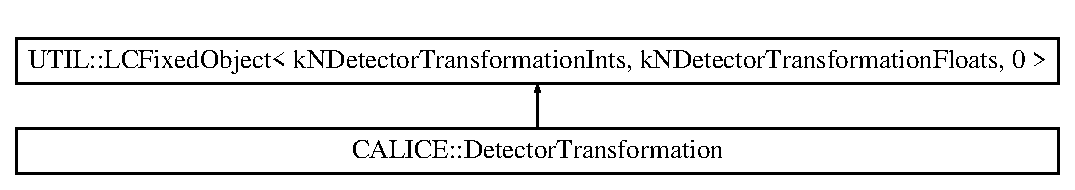
\includegraphics[height=2.000000cm]{classCALICE_1_1DetectorTransformation}
\end{center}
\end{figure}
\subsection*{Public Member Functions}
\begin{DoxyCompactItemize}
\item 
{\bf Detector\-Transformation} (L\-C\-Object $\ast$obj)\label{classCALICE_1_1DetectorTransformation_aa0cecf48097264a6a6cc0af071008d0b}

\begin{DoxyCompactList}\small\item\em 'Copy constructor' needed to interpret L\-C\-Collection read from file/database. \end{DoxyCompactList}\item 
{\bf Detector\-Transformation} \& {\bf set\-Detector\-Angle\-Z\-X} (float detector\-\_\-angle\-\_\-zx)
\begin{DoxyCompactList}\small\item\em Set the angle of the detector w.\-r.\-t. \end{DoxyCompactList}\item 
float {\bf get\-Detector\-Angle\-Z\-X} () const 
\begin{DoxyCompactList}\small\item\em Get the angle of the detector w.\-r.\-t. \end{DoxyCompactList}\item 
{\bf Detector\-Transformation} \& {\bf set\-Detector\-Rotation\-X0} (float rotation\-\_\-origin\-\_\-x0)\label{classCALICE_1_1DetectorTransformation_a2eef8fc060f0844f2c58dd406e236dcf}

\begin{DoxyCompactList}\small\item\em Set the origin of the detector rotation in the Z\-X-\/plane. \end{DoxyCompactList}\item 
float {\bf get\-Detector\-Rotation\-X0} () const \label{classCALICE_1_1DetectorTransformation_afcbf82cfdf8f7e59f8eb9d0dbbcacaf2}

\begin{DoxyCompactList}\small\item\em Get the origin of the detector rotation in the Z\-X-\/plane. \end{DoxyCompactList}\item 
{\bf Detector\-Transformation} \& {\bf set\-Detector\-Rotation\-Z0} (float rotation\-\_\-origin\-\_\-z0)\label{classCALICE_1_1DetectorTransformation_aec6ee5baab95ce9cb39df88ca04e0e80}

\begin{DoxyCompactList}\small\item\em Set the origin of the detector rotation in the Z\-X-\/plane. \end{DoxyCompactList}\item 
float {\bf get\-Detector\-Rotation\-Z0} () const \label{classCALICE_1_1DetectorTransformation_afd32ba2a1636520f713cee65d6f5b5dc}

\begin{DoxyCompactList}\small\item\em Get the origin of the detector rotation in the Z\-X-\/plane. \end{DoxyCompactList}\item 
{\bf Detector\-Transformation} \& {\bf set\-Detector\-Transformation} (float origin\-\_\-x0, float origin\-\_\-y0, float origin\-\_\-z0)\label{classCALICE_1_1DetectorTransformation_aff20896660ff50a94ffe067ccdc56ac6}

\begin{DoxyCompactList}\small\item\em Set the origin of the detector in the 3\-D-\/space (convenience method). \end{DoxyCompactList}\item 
{\bf Detector\-Transformation} \& {\bf set\-Detector\-Transformation} (float $\ast$origin\-\_\-three\-\_\-vector)\label{classCALICE_1_1DetectorTransformation_ae390bbf318d5747c72d77b6cd364540b}

\begin{DoxyCompactList}\small\item\em Set the origin of the detector in the 3\-D-\/space (convenience method). \end{DoxyCompactList}\item 
{\bf Detector\-Transformation} \& {\bf set\-Detector\-X0} (float origin\-\_\-x0)\label{classCALICE_1_1DetectorTransformation_a12be9cd46f36fbd4995afb93b0001630}

\begin{DoxyCompactList}\small\item\em Set the origin of the detector in the 3\-D-\/space. \end{DoxyCompactList}\item 
float {\bf get\-Detector\-X0} () const \label{classCALICE_1_1DetectorTransformation_ad3b792347abe29df128864f8d93db90b}

\begin{DoxyCompactList}\small\item\em Get the origin of the detector in the 3\-D-\/space. \end{DoxyCompactList}\item 
{\bf Detector\-Transformation} \& {\bf set\-Detector\-Y0} (float origin\-\_\-y0)\label{classCALICE_1_1DetectorTransformation_a8aa19f83e78ce547f6144b0ca055f5b4}

\begin{DoxyCompactList}\small\item\em Set the origin of the detector in the 3\-D-\/space. \end{DoxyCompactList}\item 
float {\bf get\-Detector\-Y0} () const \label{classCALICE_1_1DetectorTransformation_a8b40f70eab9c5f3f7246d881757fc8e9}

\begin{DoxyCompactList}\small\item\em Get the origin of the detector in the 3\-D-\/space. \end{DoxyCompactList}\item 
{\bf Detector\-Transformation} \& {\bf set\-Detector\-Z0} (float origin\-\_\-z0)\label{classCALICE_1_1DetectorTransformation_a74831156933ee18369f6ea48d90e8f29}

\begin{DoxyCompactList}\small\item\em Set the origin of the detector in the 3\-D-\/space. \end{DoxyCompactList}\item 
float {\bf get\-Detector\-Z0} () const \label{classCALICE_1_1DetectorTransformation_aed697370c5d136d4424867598c79421d}

\begin{DoxyCompactList}\small\item\em Get the origin of the detector in the 3\-D-\/space. \end{DoxyCompactList}\item 
void {\bf print} (std\-::ostream \&os)\label{classCALICE_1_1DetectorTransformation_a53146e49344a9995016d521d423959fc}

\begin{DoxyCompactList}\small\item\em Print all members (for debugging) \end{DoxyCompactList}\item 
const std\-::string {\bf get\-Type\-Name} () const \label{classCALICE_1_1DetectorTransformation_a32750bb0d4ebc5fe3a62871a4b6a427a}

\begin{DoxyCompactList}\small\item\em Return the type of the class. \end{DoxyCompactList}\item 
const std\-::string {\bf get\-Data\-Description} () const \label{classCALICE_1_1DetectorTransformation_a5c2acba9e28ad26da43444e39bc220a7}

\begin{DoxyCompactList}\small\item\em Return a brief description of the data members. \end{DoxyCompactList}\end{DoxyCompactItemize}


\subsection{Detailed Description}
Define the experimental setup\-: beam energy, position, angle and detector position, angle. 

The experimental setup should be written into the conditions database at least twice\-: 
\begin{DoxyItemize}
\item the nominal values with the tag N\-O\-M\-I\-N\-A\-L 
\item the measured values 
\end{DoxyItemize}\begin{DoxyRefDesc}{Todo}
\item[{\bf Todo}]\{Should this class be split into two? One for the beam and one for the detector parameters? Should the nominal and measured values be stored in separate folders?\} \end{DoxyRefDesc}


Definition at line 37 of file Detector\-Transformation.\-hh.



\subsection{Member Function Documentation}
\index{C\-A\-L\-I\-C\-E\-::\-Detector\-Transformation@{C\-A\-L\-I\-C\-E\-::\-Detector\-Transformation}!get\-Detector\-Angle\-Z\-X@{get\-Detector\-Angle\-Z\-X}}
\index{get\-Detector\-Angle\-Z\-X@{get\-Detector\-Angle\-Z\-X}!CALICE::DetectorTransformation@{C\-A\-L\-I\-C\-E\-::\-Detector\-Transformation}}
\subsubsection[{get\-Detector\-Angle\-Z\-X}]{\setlength{\rightskip}{0pt plus 5cm}float C\-A\-L\-I\-C\-E\-::\-Detector\-Transformation\-::get\-Detector\-Angle\-Z\-X (
\begin{DoxyParamCaption}
{}
\end{DoxyParamCaption}
) const\hspace{0.3cm}{\ttfamily [inline]}}\label{classCALICE_1_1DetectorTransformation_a457ff79d33057315b535678a89c93baa}


Get the angle of the detector w.\-r.\-t. 

z-\/axis in the Z\-X-\/plane. 

Definition at line 56 of file Detector\-Transformation.\-hh.



References C\-A\-L\-I\-C\-E\-::k\-Detector\-Transformation\-Float\-Detector\-Angle\-Z\-X.



Referenced by C\-A\-L\-I\-C\-E\-::\-Cell\-Description\-Generator\-::generate(), and print().

\index{C\-A\-L\-I\-C\-E\-::\-Detector\-Transformation@{C\-A\-L\-I\-C\-E\-::\-Detector\-Transformation}!set\-Detector\-Angle\-Z\-X@{set\-Detector\-Angle\-Z\-X}}
\index{set\-Detector\-Angle\-Z\-X@{set\-Detector\-Angle\-Z\-X}!CALICE::DetectorTransformation@{C\-A\-L\-I\-C\-E\-::\-Detector\-Transformation}}
\subsubsection[{set\-Detector\-Angle\-Z\-X}]{\setlength{\rightskip}{0pt plus 5cm}{\bf Detector\-Transformation}\& C\-A\-L\-I\-C\-E\-::\-Detector\-Transformation\-::set\-Detector\-Angle\-Z\-X (
\begin{DoxyParamCaption}
\item[{float}]{detector\-\_\-angle\-\_\-zx}
\end{DoxyParamCaption}
)\hspace{0.3cm}{\ttfamily [inline]}}\label{classCALICE_1_1DetectorTransformation_abda40c896fba1eb47056f69774f058b0}


Set the angle of the detector w.\-r.\-t. 

z-\/axis in the Z\-X-\/plane. 

Definition at line 48 of file Detector\-Transformation.\-hh.



References C\-A\-L\-I\-C\-E\-::k\-Detector\-Transformation\-Float\-Detector\-Angle\-Z\-X.



The documentation for this class was generated from the following files\-:\begin{DoxyCompactItemize}
\item 
Detector\-Transformation.\-hh\item 
Detector\-Transformation.\-cc\end{DoxyCompactItemize}

\section{C\-A\-L\-I\-C\-E\-:\-:Dhc\-Raw\-Chip\-Content Class Reference}
\label{classCALICE_1_1DhcRawChipContent}\index{C\-A\-L\-I\-C\-E\-::\-Dhc\-Raw\-Chip\-Content@{C\-A\-L\-I\-C\-E\-::\-Dhc\-Raw\-Chip\-Content}}


Simple class which stores the dhcal chip content Note that the dchal as it is now delivers the same time stamp for {\itshape all} 64 channels served by a chip.  




{\ttfamily \#include $<$Dhc\-Raw\-Chip\-Content.\-hh$>$}

Inheritance diagram for C\-A\-L\-I\-C\-E\-:\-:Dhc\-Raw\-Chip\-Content\-:\begin{figure}[H]
\begin{center}
\leavevmode
\includegraphics[height=3.000000cm]{classCALICE_1_1DhcRawChipContent}
\end{center}
\end{figure}
\subsection*{Public Member Functions}
\begin{DoxyCompactItemize}
\item 
{\bf Dhc\-Raw\-Chip\-Content} ()\label{classCALICE_1_1DhcRawChipContent_a40a38cc72c861a07276425e293834915}

\begin{DoxyCompactList}\small\item\em Simple Constructor. \end{DoxyCompactList}\item 
{\bf Dhc\-Raw\-Chip\-Content} (L\-C\-Object $\ast${\bf obj})
\begin{DoxyCompactList}\small\item\em 'Copy constructor' needed to interpret L\-C\-Collection read from file/database. \end{DoxyCompactList}\item 
virtual {\bf $\sim$\-Dhc\-Raw\-Chip\-Content} ()\label{classCALICE_1_1DhcRawChipContent_a118479e64dcaa1578df4c2b5b5305fc5}

\begin{DoxyCompactList}\small\item\em The destructor. \end{DoxyCompactList}\item 
{\bf Dhc\-Raw\-Chip\-Content} \& {\bf set\-Crate\-Number} (unsigned int cratenr)\label{classCALICE_1_1DhcRawChipContent_ae648a73206346a7e435b190c31503533}

\begin{DoxyCompactList}\small\item\em Set the high hits. \end{DoxyCompactList}\item 
unsigned int {\bfseries get\-Crate\-Number} () const \label{classCALICE_1_1DhcRawChipContent_ac38db7829bb2e4ce117bf6bff30b5e30}

\item 
{\bf Dhc\-Raw\-Chip\-Content} \& {\bf set\-Elec\-Channel} (unsigned int vmead, unsigned int dcalad, unsigned int dcolad, unsigned int dconad)\label{classCALICE_1_1DhcRawChipContent_ad15611d95fe8f56da1df10bafd42a869}

\begin{DoxyCompactList}\small\item\em Set the electronic channel number. \end{DoxyCompactList}\item 
int {\bf get\-Elec\-Channel} () const \label{classCALICE_1_1DhcRawChipContent_a835846130132c03bd9c55a52fcca0baf}

\begin{DoxyCompactList}\small\item\em Get the entire electronic channel number. \end{DoxyCompactList}\item 
unsigned int {\bf get\-Vme\-Address} () const \label{classCALICE_1_1DhcRawChipContent_a41b24b4a3aab879318b7bb73bc0abf3d}

\begin{DoxyCompactList}\small\item\em Return the addresses of individual hardware components. \end{DoxyCompactList}\item 
unsigned int {\bfseries get\-Dcal\-Address} () const \label{classCALICE_1_1DhcRawChipContent_a7c3eeeebac537abaa903e594c2719eb5}

\item 
unsigned int {\bfseries get\-Dcol\-Address} () const \label{classCALICE_1_1DhcRawChipContent_a69c7bd11fccade453f965629bf664dd7}

\item 
unsigned int {\bfseries get\-Dcon\-Address} () const \label{classCALICE_1_1DhcRawChipContent_a17b53680be279714c856302fd1932bc0}

\item 
{\bf Dhc\-Raw\-Chip\-Content} \& {\bf set\-Hits\-Hi} (unsigned int hitshi)\label{classCALICE_1_1DhcRawChipContent_a65d1a25cfdca13308dfdd0e1b101c468}

\begin{DoxyCompactList}\small\item\em Set the high hits. \end{DoxyCompactList}\item 
unsigned int {\bfseries get\-Hits\-Hi} () const \label{classCALICE_1_1DhcRawChipContent_a154d9d95875b10420c5c3bab19098e47}

\item 
{\bf Dhc\-Raw\-Chip\-Content} \& {\bf set\-Hits\-Lo} (unsigned int hitslo)\label{classCALICE_1_1DhcRawChipContent_a8a0aa0c0b062f58866ad6d8c6d641652}

\begin{DoxyCompactList}\small\item\em Set the low hits. \end{DoxyCompactList}\item 
unsigned int {\bf get\-Hits\-Lo} () const \label{classCALICE_1_1DhcRawChipContent_a41c5e80b718bb2aaf5367c5506bf5f1d}

\begin{DoxyCompactList}\small\item\em Return the low hits. \end{DoxyCompactList}\item 
{\bf Dhc\-Raw\-Chip\-Content} \& {\bf set\-Dhc\-Time\-Stamp} (unsigned int timestamp)\label{classCALICE_1_1DhcRawChipContent_ac0e10fb580cc00b0f4b0a3efdd956b91}

\begin{DoxyCompactList}\small\item\em The core, the time stamp. \end{DoxyCompactList}\item 
unsigned int {\bf get\-Dhc\-Time\-Stamp} () const \label{classCALICE_1_1DhcRawChipContent_a784ab74d557fa360154d0116f8448d03}

\begin{DoxyCompactList}\small\item\em Return the time stamp. \end{DoxyCompactList}\item 
{\bf Dhc\-Raw\-Chip\-Content} \& {\bf set\-Misc\-Info} (bool trg, bool dbt, unsigned char err, unsigned char chksum, unsigned char versum)\label{classCALICE_1_1DhcRawChipContent_abed887f844826b95fe369701a8b6719d}

\begin{DoxyCompactList}\small\item\em Set miscalleneous information. \end{DoxyCompactList}\item 
bool {\bf get\-Trg\-Info} ()\label{classCALICE_1_1DhcRawChipContent_a7c93aa3a5eb24d81067e2d4059869435}

\begin{DoxyCompactList}\small\item\em Return the trigger information. \end{DoxyCompactList}\item 
bool {\bf get\-Dbt\-Info} ()\label{classCALICE_1_1DhcRawChipContent_a26fb65c45f4a3b07d779e442069477f2}

\begin{DoxyCompactList}\small\item\em Return the dbt information. \end{DoxyCompactList}\item 
unsigned char {\bf get\-Err\-Info} ()\label{classCALICE_1_1DhcRawChipContent_af6261bc47ae47a360632fb0079d4bc99}

\begin{DoxyCompactList}\small\item\em Return the error information. \end{DoxyCompactList}\item 
unsigned char {\bf get\-Chk\-Sum} ()\label{classCALICE_1_1DhcRawChipContent_aa9a55ba4880c7b03db55c3728980f44d}

\begin{DoxyCompactList}\small\item\em Return the checksum information. \end{DoxyCompactList}\item 
unsigned char {\bf get\-Ver\-Sum} ()\label{classCALICE_1_1DhcRawChipContent_a469cbbfed09f4f5a7e1bc3775b6240e9}

\begin{DoxyCompactList}\small\item\em Return the verification sum (to check checksum) \end{DoxyCompactList}\item 
std\-::ostream \& {\bf print} (std\-::ostream \&ostrm)\label{classCALICE_1_1DhcRawChipContent_a555dbb9e80d6bb86d0d0092231109ebe}

\begin{DoxyCompactList}\small\item\em Convenient print method. \end{DoxyCompactList}\item 
const std\-::string {\bfseries get\-Type\-Name} () const \label{classCALICE_1_1DhcRawChipContent_a3a5fd3f86e153a64edcbeb444001f5aa}

\item 
const std\-::string {\bf get\-Data\-Description} () const \label{classCALICE_1_1DhcRawChipContent_af28eebdb0ad0ce1f8be17f191b714ef0}

\begin{DoxyCompactList}\small\item\em Return a brief description of the data members. \end{DoxyCompactList}\end{DoxyCompactItemize}
\subsection*{Additional Inherited Members}


\subsection{Detailed Description}
Simple class which stores the dhcal chip content Note that the dchal as it is now delivers the same time stamp for {\itshape all} 64 channels served by a chip. 

That's why the L\-C\-I\-O Raw\-Calorimeter\-Hit class is not convenient. Since it would lead to an increas of the data volume by a factor 64.

\begin{DoxyAuthor}{Author}
R. P�schl (L\-A\-L Orsay) 
\end{DoxyAuthor}
\begin{DoxyDate}{Date}
Dec 2010 
\end{DoxyDate}


Definition at line 56 of file Dhc\-Raw\-Chip\-Content.\-hh.



\subsection{Constructor \& Destructor Documentation}
\index{C\-A\-L\-I\-C\-E\-::\-Dhc\-Raw\-Chip\-Content@{C\-A\-L\-I\-C\-E\-::\-Dhc\-Raw\-Chip\-Content}!Dhc\-Raw\-Chip\-Content@{Dhc\-Raw\-Chip\-Content}}
\index{Dhc\-Raw\-Chip\-Content@{Dhc\-Raw\-Chip\-Content}!CALICE::DhcRawChipContent@{C\-A\-L\-I\-C\-E\-::\-Dhc\-Raw\-Chip\-Content}}
\subsubsection[{Dhc\-Raw\-Chip\-Content}]{\setlength{\rightskip}{0pt plus 5cm}C\-A\-L\-I\-C\-E\-::\-Dhc\-Raw\-Chip\-Content\-::\-Dhc\-Raw\-Chip\-Content (
\begin{DoxyParamCaption}
\item[{L\-C\-Object $\ast$}]{obj}
\end{DoxyParamCaption}
)\hspace{0.3cm}{\ttfamily [inline]}}\label{classCALICE_1_1DhcRawChipContent_aa7c59fb4dd3447fb4968bff83ae2e72d}


'Copy constructor' needed to interpret L\-C\-Collection read from file/database. 



Definition at line 73 of file Dhc\-Raw\-Chip\-Content.\-hh.



The documentation for this class was generated from the following files\-:\begin{DoxyCompactItemize}
\item 
Dhc\-Raw\-Chip\-Content.\-hh\item 
Dhc\-Raw\-Chip\-Content.\-cc\end{DoxyCompactItemize}

\section{C\-A\-L\-I\-C\-E\-:\-:Dhc\-Readout\-Conf\-Block Class Reference}
\label{classCALICE_1_1DhcReadoutConfBlock}\index{C\-A\-L\-I\-C\-E\-::\-Dhc\-Readout\-Conf\-Block@{C\-A\-L\-I\-C\-E\-::\-Dhc\-Readout\-Conf\-Block}}


Class to interface the configuration of the Dhcal fes.  




{\ttfamily \#include $<$Dhc\-Readout\-Conf\-Block.\-hh$>$}

Inheritance diagram for C\-A\-L\-I\-C\-E\-:\-:Dhc\-Readout\-Conf\-Block\-:\begin{figure}[H]
\begin{center}
\leavevmode
\includegraphics[height=3.000000cm]{classCALICE_1_1DhcReadoutConfBlock}
\end{center}
\end{figure}
\subsection*{Public Member Functions}
\begin{DoxyCompactItemize}
\item 
{\bf Dhc\-Readout\-Conf\-Block} ()\label{classCALICE_1_1DhcReadoutConfBlock_a70a6203130f321b808bfd840623d9e7f}

\begin{DoxyCompactList}\small\item\em Simple Constructor. \end{DoxyCompactList}\item 
{\bf Dhc\-Readout\-Conf\-Block} (L\-C\-Object $\ast${\bf obj})
\begin{DoxyCompactList}\small\item\em 'Copy constructor' needed to interpret L\-C\-Collection read from file/database. \end{DoxyCompactList}\item 
virtual {\bf $\sim$\-Dhc\-Readout\-Conf\-Block} ()\label{classCALICE_1_1DhcReadoutConfBlock_a1765688be6fb5c820ad7403b700b4462}

\begin{DoxyCompactList}\small\item\em The destructor. \end{DoxyCompactList}\item 
{\bf Dhc\-Readout\-Conf\-Block} \& {\bf set\-Numbers} (unsigned int numbers)\label{classCALICE_1_1DhcReadoutConfBlock_ae23cae3a4b8e9a5390e67a8a9022d401}

\begin{DoxyCompactList}\small\item\em Set the numbers. \end{DoxyCompactList}\item 
unsigned int {\bf get\-Numbers} () const \label{classCALICE_1_1DhcReadoutConfBlock_a9f32a07abeb6b9231c893af87d489458}

\begin{DoxyCompactList}\small\item\em Get the numbers. \end{DoxyCompactList}\item 
unsigned int {\bf get\-Crate\-Number} ()\label{classCALICE_1_1DhcReadoutConfBlock_a780bef3bacec82f4b3526eb27c2d7115}

\begin{DoxyCompactList}\small\item\em Return the crate number, can be obtained from numbers. \end{DoxyCompactList}\item 
{\bf Dhc\-Readout\-Conf\-Block} \& {\bf set\-Slot\-Enable\-Mask} (unsigned int slotenablemask)\label{classCALICE_1_1DhcReadoutConfBlock_afa415eb6133bf1c69058c298322770d6}

\begin{DoxyCompactList}\small\item\em Set the slot enable mask, which tells which slots in could (in principle) have been enabled. \end{DoxyCompactList}\item 
unsigned int {\bf get\-Slot\-Enable\-Mask} () const \label{classCALICE_1_1DhcReadoutConfBlock_af6c73aac10efdf9b040b3f7c129b460d}

\begin{DoxyCompactList}\small\item\em Get the slot enable mask. \end{DoxyCompactList}\item 
{\bf Dhc\-Readout\-Conf\-Block} \& {\bf set\-Slot\-Enable} (unsigned int slotenable)
\begin{DoxyCompactList}\small\item\em Set the slot enable, i.\-e. \end{DoxyCompactList}\item 
unsigned int {\bf get\-Slot\-Enable} () const \label{classCALICE_1_1DhcReadoutConfBlock_a3b7ff51d37ea0eb0d9fd28483d4f4d05}

\begin{DoxyCompactList}\small\item\em Get the slot enable. \end{DoxyCompactList}\item 
{\bf Dhc\-Readout\-Conf\-Block} \& {\bf set\-Number\-Of\-Slots} (unsigned int numslots)\label{classCALICE_1_1DhcReadoutConfBlock_aa8c67bc9f9b615951ffaeb1322780870}

\begin{DoxyCompactList}\small\item\em Set the number of slots, note that this number will have to be multiplied by two, leave it for the time being. \end{DoxyCompactList}\item 
unsigned int {\bf get\-Number\-Of\-Slots} () const \label{classCALICE_1_1DhcReadoutConfBlock_ade3ff579b72a62e49ffb1ac2eb5d4af0}

\begin{DoxyCompactList}\small\item\em Get the numbers of slots. \end{DoxyCompactList}\item 
{\bf Dhc\-Readout\-Conf\-Block} \& {\bf set\-Slot\-Fe\-Enable} (unsigned int islot, unsigned int val)\label{classCALICE_1_1DhcReadoutConfBlock_a86d81715bb55e049b0165413b5dd78e7}

\begin{DoxyCompactList}\small\item\em Set the enabled fes for this slot. \end{DoxyCompactList}\item 
unsigned short {\bf get\-Slot\-Fe\-Enable} (unsigned int islot)\label{classCALICE_1_1DhcReadoutConfBlock_a6dfd32e97665265a42e265be9adaad72}

\begin{DoxyCompactList}\small\item\em Get the enabled fes for this slot. \end{DoxyCompactList}\item 
{\bf Dhc\-Readout\-Conf\-Block} \& {\bf set\-Slot\-Fe\-Revision} (unsigned int islot, unsigned char val)\label{classCALICE_1_1DhcReadoutConfBlock_a50394d95d1b8a5645fd20aea51eab985}

\begin{DoxyCompactList}\small\item\em Set the revision number of the fes for this slot. \end{DoxyCompactList}\item 
unsigned char {\bf get\-Slot\-Fe\-Revision} (unsigned int islot)\label{classCALICE_1_1DhcReadoutConfBlock_a6e3a476cb7b0bfb8f873f560061ac359}

\begin{DoxyCompactList}\small\item\em Set the revision number of the fes for this slot. \end{DoxyCompactList}\item 
{\bf Dhc\-Readout\-Conf\-Block} \& {\bf set\-Be\-Wait\-Interval} (unsigned int timeinmus)\label{classCALICE_1_1DhcReadoutConfBlock_a2c55d4268e15f6d729b6c137e84a7ce9}

\begin{DoxyCompactList}\small\item\em Set the Be wait interval. \end{DoxyCompactList}\item 
L\-C\-Time {\bf get\-Be\-Wait\-Interval} ()\label{classCALICE_1_1DhcReadoutConfBlock_aee430b699617c6f5455097a665d479dd}

\begin{DoxyCompactList}\small\item\em Return the Be wait interval, in mus. \end{DoxyCompactList}\item 
std\-::ostream \& {\bf print} (std\-::ostream \&ostrm)\label{classCALICE_1_1DhcReadoutConfBlock_a8ee86e4066e289a3b7c8ac19af5cb45c}

\begin{DoxyCompactList}\small\item\em Convenient print method. \end{DoxyCompactList}\item 
const std\-::string {\bfseries get\-Type\-Name} () const \label{classCALICE_1_1DhcReadoutConfBlock_a634f76ea5b591f421b31605ef247b1c4}

\item 
const std\-::string {\bf get\-Data\-Description} () const \label{classCALICE_1_1DhcReadoutConfBlock_a13be0777aff947ce444b20b25b53720e}

\begin{DoxyCompactList}\small\item\em Return a brief description of the data members. \end{DoxyCompactList}\end{DoxyCompactItemize}
\subsection*{Private Member Functions}
\begin{DoxyCompactItemize}
\item 
void {\bf fill\-Slot\-To\-Words\-Association\-Mask} (unsigned int, bool)
\begin{DoxyCompactList}\small\item\em Association mask. \end{DoxyCompactList}\item 
void {\bf fill\-Method} (unsigned int, unsigned int, unsigned int, unsigned int)\label{classCALICE_1_1DhcReadoutConfBlock_a593c9ef319474740dba7dc0c723d5dac}

\begin{DoxyCompactList}\small\item\em A convenient method to fill fe eanble and fe revision values. \end{DoxyCompactList}\item 
unsigned short {\bf get\-Method} (unsigned int, unsigned int, unsigned int)\label{classCALICE_1_1DhcReadoutConfBlock_a7b5d00a1093812e7eee3fc1a67798138}

\begin{DoxyCompactList}\small\item\em A convenient method to fill fe eanble and fe revision values. \end{DoxyCompactList}\end{DoxyCompactItemize}
\subsection*{Private Attributes}
\begin{DoxyCompactItemize}
\item 
std\-::map$<$ unsigned int, \\*
unsigned int $>$ {\bf \-\_\-islotfill\-Map}\label{classCALICE_1_1DhcReadoutConfBlock_abce693038d694ce51fb6cde002c4dd60}

\begin{DoxyCompactList}\small\item\em map which associates the slots with the position in the L\-C\-Generic\-Object \end{DoxyCompactList}\item 
bool {\bf \-\_\-num\-Slots\-Initialised}\label{classCALICE_1_1DhcReadoutConfBlock_ae767a99973ecf078a438c5c80e4f3019}

\begin{DoxyCompactList}\small\item\em is the number of slots initialised (makes only sense during the filling sequence) \end{DoxyCompactList}\end{DoxyCompactItemize}
\subsection*{Additional Inherited Members}


\subsection{Detailed Description}
Class to interface the configuration of the Dhcal fes. 

\begin{DoxyAuthor}{Author}
R. P�schl (L\-A\-L Orsay), J. Smith (A\-N\-L) 
\end{DoxyAuthor}
\begin{DoxyDate}{Date}
Apr 2011 
\end{DoxyDate}
\begin{DoxyRefDesc}{Todo}
\item[{\bf Todo}]Attention we may introduce a platform dependency here!!!! The structure of the object assumes that L\-C\-Generic\-Objects are aligned on 32 bits Need maybe revision for assumptions on data alignment, could be added as collection parameters, \end{DoxyRefDesc}


Definition at line 32 of file Dhc\-Readout\-Conf\-Block.\-hh.



\subsection{Constructor \& Destructor Documentation}
\index{C\-A\-L\-I\-C\-E\-::\-Dhc\-Readout\-Conf\-Block@{C\-A\-L\-I\-C\-E\-::\-Dhc\-Readout\-Conf\-Block}!Dhc\-Readout\-Conf\-Block@{Dhc\-Readout\-Conf\-Block}}
\index{Dhc\-Readout\-Conf\-Block@{Dhc\-Readout\-Conf\-Block}!CALICE::DhcReadoutConfBlock@{C\-A\-L\-I\-C\-E\-::\-Dhc\-Readout\-Conf\-Block}}
\subsubsection[{Dhc\-Readout\-Conf\-Block}]{\setlength{\rightskip}{0pt plus 5cm}C\-A\-L\-I\-C\-E\-::\-Dhc\-Readout\-Conf\-Block\-::\-Dhc\-Readout\-Conf\-Block (
\begin{DoxyParamCaption}
\item[{L\-C\-Object $\ast$}]{obj}
\end{DoxyParamCaption}
)\hspace{0.3cm}{\ttfamily [inline]}}\label{classCALICE_1_1DhcReadoutConfBlock_a7d4faa50c5595058596fde44971854ab}


'Copy constructor' needed to interpret L\-C\-Collection read from file/database. 



Definition at line 48 of file Dhc\-Readout\-Conf\-Block.\-hh.



\subsection{Member Function Documentation}
\index{C\-A\-L\-I\-C\-E\-::\-Dhc\-Readout\-Conf\-Block@{C\-A\-L\-I\-C\-E\-::\-Dhc\-Readout\-Conf\-Block}!fill\-Slot\-To\-Words\-Association\-Mask@{fill\-Slot\-To\-Words\-Association\-Mask}}
\index{fill\-Slot\-To\-Words\-Association\-Mask@{fill\-Slot\-To\-Words\-Association\-Mask}!CALICE::DhcReadoutConfBlock@{C\-A\-L\-I\-C\-E\-::\-Dhc\-Readout\-Conf\-Block}}
\subsubsection[{fill\-Slot\-To\-Words\-Association\-Mask}]{\setlength{\rightskip}{0pt plus 5cm}void Dhc\-Readout\-Conf\-Block\-::fill\-Slot\-To\-Words\-Association\-Mask (
\begin{DoxyParamCaption}
\item[{unsigned int}]{slotenablemask, }
\item[{bool}]{initvals}
\end{DoxyParamCaption}
)\hspace{0.3cm}{\ttfamily [private]}}\label{classCALICE_1_1DhcReadoutConfBlock_ae090fa9e9abbbd1156220bff23b0293c}


Association mask. 

using the slot enable mask we create the map which associates the slots to the position in the L\-C\-Generic\-Object 

Definition at line 21 of file Dhc\-Readout\-Conf\-Block.\-cc.



References \-\_\-islotfill\-Map, \-\_\-num\-Slots\-Initialised, get\-Number\-Of\-Slots(), and C\-A\-L\-I\-C\-E\-::\-L\-C\-Generic\-Object\-Impl\-Ext\-::obj().

\index{C\-A\-L\-I\-C\-E\-::\-Dhc\-Readout\-Conf\-Block@{C\-A\-L\-I\-C\-E\-::\-Dhc\-Readout\-Conf\-Block}!set\-Slot\-Enable@{set\-Slot\-Enable}}
\index{set\-Slot\-Enable@{set\-Slot\-Enable}!CALICE::DhcReadoutConfBlock@{C\-A\-L\-I\-C\-E\-::\-Dhc\-Readout\-Conf\-Block}}
\subsubsection[{set\-Slot\-Enable}]{\setlength{\rightskip}{0pt plus 5cm}{\bf Dhc\-Readout\-Conf\-Block}\& C\-A\-L\-I\-C\-E\-::\-Dhc\-Readout\-Conf\-Block\-::set\-Slot\-Enable (
\begin{DoxyParamCaption}
\item[{unsigned int}]{slotenable}
\end{DoxyParamCaption}
)\hspace{0.3cm}{\ttfamily [inline]}}\label{classCALICE_1_1DhcReadoutConfBlock_a3c77ac14bc825e8e14ec2346547c5ce4}


Set the slot enable, i.\-e. 

the slots which are really enabled 

Definition at line 92 of file Dhc\-Readout\-Conf\-Block.\-hh.



The documentation for this class was generated from the following files\-:\begin{DoxyCompactItemize}
\item 
Dhc\-Readout\-Conf\-Block.\-hh\item 
Dhc\-Readout\-Conf\-Block.\-cc\end{DoxyCompactItemize}

\section{C\-A\-L\-I\-C\-E\-:\-:Dif\-Trigger Class Reference}
\label{classCALICE_1_1DifTrigger}\index{C\-A\-L\-I\-C\-E\-::\-Dif\-Trigger@{C\-A\-L\-I\-C\-E\-::\-Dif\-Trigger}}


Simple class which stores the trigger counter retrieved from the D\-I\-F cards.  




{\ttfamily \#include $<$Dif\-Trigger.\-hh$>$}

Inheritance diagram for C\-A\-L\-I\-C\-E\-:\-:Dif\-Trigger\-:\begin{figure}[H]
\begin{center}
\leavevmode
\includegraphics[height=3.000000cm]{classCALICE_1_1DifTrigger}
\end{center}
\end{figure}
\subsection*{Public Member Functions}
\begin{DoxyCompactItemize}
\item 
{\bf Dif\-Trigger} ()\label{classCALICE_1_1DifTrigger_a6b7e84ec0cf67f3aea3f44e32ab976f1}

\begin{DoxyCompactList}\small\item\em Simple Constructor. \end{DoxyCompactList}\item 
{\bf Dif\-Trigger} (L\-C\-Object $\ast${\bf obj})
\begin{DoxyCompactList}\small\item\em 'Copy constructor' needed to interpret L\-C\-Collection read from file/database. \end{DoxyCompactList}\item 
virtual {\bf $\sim$\-Dif\-Trigger} ()\label{classCALICE_1_1DifTrigger_abb5e9c8b0f17ad4a0dc0885640ede48f}

\begin{DoxyCompactList}\small\item\em The destructor. \end{DoxyCompactList}\item 
{\bf Dif\-Trigger} \& {\bf set\-Trigger\-Counter} (int triggercounter)\label{classCALICE_1_1DifTrigger_abed77f4943569ab3e5e1abf1280f7fe5}

\begin{DoxyCompactList}\small\item\em Set the trigger counter. \end{DoxyCompactList}\item 
int {\bf get\-Trigger\-Counter} () const \label{classCALICE_1_1DifTrigger_a1a369c606a8c7a935c10f154b8d8f967}

\begin{DoxyCompactList}\small\item\em Get the trigger counter. \end{DoxyCompactList}\item 
std\-::ostream \& {\bf print} (std\-::ostream \&ostrm)\label{classCALICE_1_1DifTrigger_aa029e99b0d09472495e640a1a10bcf27}

\begin{DoxyCompactList}\small\item\em Convenient print method. \end{DoxyCompactList}\item 
const std\-::string {\bfseries get\-Type\-Name} () const \label{classCALICE_1_1DifTrigger_abdf381d1c077acd671f35d18d69a7b1a}

\item 
const std\-::string {\bf get\-Data\-Description} () const \label{classCALICE_1_1DifTrigger_a24d4a28eb189d634f917db3152340d5a}

\begin{DoxyCompactList}\small\item\em Return a brief description of the data members. \end{DoxyCompactList}\end{DoxyCompactItemize}
\subsection*{Additional Inherited Members}


\subsection{Detailed Description}
Simple class which stores the trigger counter retrieved from the D\-I\-F cards. 

\begin{DoxyAuthor}{Author}
R. P�schl (L\-A\-L Orsay) 
\end{DoxyAuthor}
\begin{DoxyDate}{Date}
Dec 2010 
\end{DoxyDate}


Definition at line 24 of file Dif\-Trigger.\-hh.



\subsection{Constructor \& Destructor Documentation}
\index{C\-A\-L\-I\-C\-E\-::\-Dif\-Trigger@{C\-A\-L\-I\-C\-E\-::\-Dif\-Trigger}!Dif\-Trigger@{Dif\-Trigger}}
\index{Dif\-Trigger@{Dif\-Trigger}!CALICE::DifTrigger@{C\-A\-L\-I\-C\-E\-::\-Dif\-Trigger}}
\subsubsection[{Dif\-Trigger}]{\setlength{\rightskip}{0pt plus 5cm}C\-A\-L\-I\-C\-E\-::\-Dif\-Trigger\-::\-Dif\-Trigger (
\begin{DoxyParamCaption}
\item[{L\-C\-Object $\ast$}]{obj}
\end{DoxyParamCaption}
)\hspace{0.3cm}{\ttfamily [inline]}}\label{classCALICE_1_1DifTrigger_a7edb32f4d6666697091f3c844f253da2}


'Copy constructor' needed to interpret L\-C\-Collection read from file/database. 



Definition at line 33 of file Dif\-Trigger.\-hh.



The documentation for this class was generated from the following files\-:\begin{DoxyCompactItemize}
\item 
Dif\-Trigger.\-hh\item 
Dif\-Trigger.\-cc\end{DoxyCompactItemize}

\section{C\-A\-L\-I\-C\-E\-:\-:Drift\-Chamber\-Parameter Class Reference}
\label{classCALICE_1_1DriftChamberParameter}\index{C\-A\-L\-I\-C\-E\-::\-Drift\-Chamber\-Parameter@{C\-A\-L\-I\-C\-E\-::\-Drift\-Chamber\-Parameter}}


Parameters for one drift chamber.  




{\ttfamily \#include $<$Drift\-Chamber\-Parameter.\-hh$>$}

Inheritance diagram for C\-A\-L\-I\-C\-E\-:\-:Drift\-Chamber\-Parameter\-:\begin{figure}[H]
\begin{center}
\leavevmode
\includegraphics[height=2.000000cm]{classCALICE_1_1DriftChamberParameter}
\end{center}
\end{figure}
\subsection*{Public Member Functions}
\begin{DoxyCompactItemize}
\item 
{\bf Drift\-Chamber\-Parameter} (L\-C\-Object $\ast$obj)\label{classCALICE_1_1DriftChamberParameter_ac3f7e30c5f70454126342fe3e192c1be}

\begin{DoxyCompactList}\small\item\em 'Copy constructor' needed to interpret L\-C\-Collection read from file/database. \end{DoxyCompactList}\item 
{\bf Drift\-Chamber\-Parameter} \& {\bf set\-Drift\-Velocity} (float drift\-\_\-velocity)\label{classCALICE_1_1DriftChamberParameter_a72ca0c60cfa34e730a99b8ebb557021f}

\begin{DoxyCompactList}\small\item\em Set the drift velocity. \end{DoxyCompactList}\item 
float {\bf get\-Drift\-Velocity} () const \label{classCALICE_1_1DriftChamberParameter_a478ffb65ebfcdba16139529f2f19ec72}

\begin{DoxyCompactList}\small\item\em Get the drift velocity. \end{DoxyCompactList}\item 
{\bf Drift\-Chamber\-Parameter} \& {\bf set\-Delay} (float time\-\_\-shift)\label{classCALICE_1_1DriftChamberParameter_a6a0f492d3b1cb14da314e777fd5796c9}

\begin{DoxyCompactList}\small\item\em Set the time to be subtracted from the measured time to get the drift time. \end{DoxyCompactList}\item 
float {\bf get\-Delay} () const \label{classCALICE_1_1DriftChamberParameter_af6f6db7b63df194db0ada6c041a3da79}

\begin{DoxyCompactList}\small\item\em Get the time to be subtracted from the measured time to get the drift time. \end{DoxyCompactList}\item 
{\bf Drift\-Chamber\-Parameter} \& {\bf set\-Offset\-Z} (float offset\-\_\-z)\label{classCALICE_1_1DriftChamberParameter_a0e43cdb564cb5929fd6785e684c83e85}

\begin{DoxyCompactList}\small\item\em Set the position offset of the chamber in the z-\/direction. \end{DoxyCompactList}\item 
float {\bf get\-Offset\-Z} () const \label{classCALICE_1_1DriftChamberParameter_a1925ac170371b9574a3b4998c4b4f1f0}

\begin{DoxyCompactList}\small\item\em Get the position offset of the chamber in the z-\/direction. \end{DoxyCompactList}\item 
{\bf Drift\-Chamber\-Parameter} \& {\bf set\-Offset\-U} (float offset\-\_\-u)\label{classCALICE_1_1DriftChamberParameter_a7f9a1ae51dfad2028a0b5993433c98cb}

\begin{DoxyCompactList}\small\item\em Set the position offset of the chamber in the drift direction. \end{DoxyCompactList}\item 
float {\bf get\-Offset\-U} () const \label{classCALICE_1_1DriftChamberParameter_a2dd08e38dd7db22ee48b0272c1903b39}

\begin{DoxyCompactList}\small\item\em Get the position offset of the chamber in the drift direction. \end{DoxyCompactList}\item 
{\bf Drift\-Chamber\-Parameter} \& {\bf set\-Error} (float error)\label{classCALICE_1_1DriftChamberParameter_a0512b63c9b0bee95b8e69d10c27ded14}

\begin{DoxyCompactList}\small\item\em Set the error on the position measurement. \end{DoxyCompactList}\item 
float {\bf get\-Error} () const \label{classCALICE_1_1DriftChamberParameter_a8e971cf949cfad6d401fa191619da841}

\begin{DoxyCompactList}\small\item\em Get the error on the position measurement. \end{DoxyCompactList}\item 
{\bf Drift\-Chamber\-Parameter} \& {\bf set\-Direction\-Sign} (int sign)\label{classCALICE_1_1DriftChamberParameter_afd5956ba2128c0f666c64122f15d9d4b}

\begin{DoxyCompactList}\small\item\em Set the sign of the drift direction. \end{DoxyCompactList}\item 
int {\bf get\-Direction\-Sign} () const \label{classCALICE_1_1DriftChamberParameter_a8ac5b85049c531796b2f2f06ad011639}

\begin{DoxyCompactList}\small\item\em Get the sign of the drift direction. \end{DoxyCompactList}\item 
float {\bf calc\-Pos} (float time) const 
\begin{DoxyCompactList}\small\item\em Calculate from the measured time the postion along the drift direction. \end{DoxyCompactList}\item 
float {\bf calc\-Time} (float pos) const 
\begin{DoxyCompactList}\small\item\em Calculate from the measured time the postion along the drift direction. \end{DoxyCompactList}\item 
float {\bf calc\-Delay} (float residual) const 
\begin{DoxyCompactList}\small\item\em Calculate from the measured residual the shift of the offset to be subtracted from the measured time. \end{DoxyCompactList}\item 
E\-Drift\-Chamber\-Wire\-Type {\bf get\-Wire\-Type} () const 
\begin{DoxyCompactList}\small\item\em Return the type of the wire. \end{DoxyCompactList}\item 
void {\bf set\-Wire\-Type} (int wire\-\_\-type)\label{classCALICE_1_1DriftChamberParameter_a9de6a8d30fab8e57684d3a7d0f00165a}

\begin{DoxyCompactList}\small\item\em Set the wire type. \end{DoxyCompactList}\item 
void {\bf print} (std\-::ostream \&os)\label{classCALICE_1_1DriftChamberParameter_ab1c4711a572d91c6baff942c93b42241}

\begin{DoxyCompactList}\small\item\em Print all members (for debugging) \end{DoxyCompactList}\item 
const std\-::string {\bf get\-Type\-Name} () const \label{classCALICE_1_1DriftChamberParameter_a20a1522331c7491a899b118af3bfb4b5}

\begin{DoxyCompactList}\small\item\em Return the type of the class. \end{DoxyCompactList}\item 
const std\-::string {\bf get\-Data\-Description} () const \label{classCALICE_1_1DriftChamberParameter_affafce2f39862cdf7bb2a757bc95b288}

\begin{DoxyCompactList}\small\item\em Return a brief description of the data members. \end{DoxyCompactList}\end{DoxyCompactItemize}


\subsection{Detailed Description}
Parameters for one drift chamber. 

Definition at line 41 of file Drift\-Chamber\-Parameter.\-hh.



\subsection{Member Function Documentation}
\index{C\-A\-L\-I\-C\-E\-::\-Drift\-Chamber\-Parameter@{C\-A\-L\-I\-C\-E\-::\-Drift\-Chamber\-Parameter}!calc\-Delay@{calc\-Delay}}
\index{calc\-Delay@{calc\-Delay}!CALICE::DriftChamberParameter@{C\-A\-L\-I\-C\-E\-::\-Drift\-Chamber\-Parameter}}
\subsubsection[{calc\-Delay}]{\setlength{\rightskip}{0pt plus 5cm}float C\-A\-L\-I\-C\-E\-::\-Drift\-Chamber\-Parameter\-::calc\-Delay (
\begin{DoxyParamCaption}
\item[{float}]{residual}
\end{DoxyParamCaption}
) const\hspace{0.3cm}{\ttfamily [inline]}}\label{classCALICE_1_1DriftChamberParameter_ab79e1f5bcf0da040c4af2b2ad23b43b5}


Calculate from the measured residual the shift of the offset to be subtracted from the measured time. 



Definition at line 163 of file Drift\-Chamber\-Parameter.\-hh.

\index{C\-A\-L\-I\-C\-E\-::\-Drift\-Chamber\-Parameter@{C\-A\-L\-I\-C\-E\-::\-Drift\-Chamber\-Parameter}!calc\-Pos@{calc\-Pos}}
\index{calc\-Pos@{calc\-Pos}!CALICE::DriftChamberParameter@{C\-A\-L\-I\-C\-E\-::\-Drift\-Chamber\-Parameter}}
\subsubsection[{calc\-Pos}]{\setlength{\rightskip}{0pt plus 5cm}float C\-A\-L\-I\-C\-E\-::\-Drift\-Chamber\-Parameter\-::calc\-Pos (
\begin{DoxyParamCaption}
\item[{float}]{time}
\end{DoxyParamCaption}
) const\hspace{0.3cm}{\ttfamily [inline]}}\label{classCALICE_1_1DriftChamberParameter_a7428fac05d35e11805d56bb8dc049f32}


Calculate from the measured time the postion along the drift direction. 



Definition at line 153 of file Drift\-Chamber\-Parameter.\-hh.

\index{C\-A\-L\-I\-C\-E\-::\-Drift\-Chamber\-Parameter@{C\-A\-L\-I\-C\-E\-::\-Drift\-Chamber\-Parameter}!calc\-Time@{calc\-Time}}
\index{calc\-Time@{calc\-Time}!CALICE::DriftChamberParameter@{C\-A\-L\-I\-C\-E\-::\-Drift\-Chamber\-Parameter}}
\subsubsection[{calc\-Time}]{\setlength{\rightskip}{0pt plus 5cm}float C\-A\-L\-I\-C\-E\-::\-Drift\-Chamber\-Parameter\-::calc\-Time (
\begin{DoxyParamCaption}
\item[{float}]{pos}
\end{DoxyParamCaption}
) const\hspace{0.3cm}{\ttfamily [inline]}}\label{classCALICE_1_1DriftChamberParameter_a8a345729460750459938502986ff4c27}


Calculate from the measured time the postion along the drift direction. 



Definition at line 158 of file Drift\-Chamber\-Parameter.\-hh.

\index{C\-A\-L\-I\-C\-E\-::\-Drift\-Chamber\-Parameter@{C\-A\-L\-I\-C\-E\-::\-Drift\-Chamber\-Parameter}!get\-Wire\-Type@{get\-Wire\-Type}}
\index{get\-Wire\-Type@{get\-Wire\-Type}!CALICE::DriftChamberParameter@{C\-A\-L\-I\-C\-E\-::\-Drift\-Chamber\-Parameter}}
\subsubsection[{get\-Wire\-Type}]{\setlength{\rightskip}{0pt plus 5cm}E\-Drift\-Chamber\-Wire\-Type C\-A\-L\-I\-C\-E\-::\-Drift\-Chamber\-Parameter\-::get\-Wire\-Type (
\begin{DoxyParamCaption}
{}
\end{DoxyParamCaption}
) const\hspace{0.3cm}{\ttfamily [inline]}}\label{classCALICE_1_1DriftChamberParameter_a056d3a2b0823518ed1fc3d184488d91a}


Return the type of the wire. 

Wires are distinguished by their orientation (x.\-y) and the position with respect to the beam axis (left or right of the beam axis for x; below or above the beam axis for y wires). 

Definition at line 172 of file Drift\-Chamber\-Parameter.\-hh.



References C\-A\-L\-I\-C\-E\-::k\-Drift\-Chamber\-Parameter\-Int\-Wire\-Type.



The documentation for this class was generated from the following files\-:\begin{DoxyCompactItemize}
\item 
Drift\-Chamber\-Parameter.\-hh\item 
Drift\-Chamber\-Parameter.\-cc\end{DoxyCompactItemize}

\section{C\-A\-L\-I\-C\-E\-:\-:E4\-D\-Mapper Class Reference}
\label{classCALICE_1_1E4DMapper}\index{C\-A\-L\-I\-C\-E\-::\-E4\-D\-Mapper@{C\-A\-L\-I\-C\-E\-::\-E4\-D\-Mapper}}


A\-H\-C\-A\-L E\-P\-T implementation of \doxyref{Mapper}{p.}{classCALICE_1_1Mapper} class Functions to get dimensions of detector geometry.  




{\ttfamily \#include $<$E4\-D\-Mapper.\-hh$>$}

\subsection*{Public Member Functions}
\begin{DoxyCompactItemize}
\item 
int {\bfseries get\-Cell\-I\-D0\-From\-I\-J\-K} (const unsigned int I, const unsigned int J, const unsigned int K) const \label{classCALICE_1_1E4DMapper_ada2c0dfde0035a60d5a751a14309cd65}

\item 
int {\bfseries get\-Cell\-I\-D0\-From\-Module\-Chip\-Channel} (const unsigned int module, const unsigned int chip, const unsigned int channel) const \label{classCALICE_1_1E4DMapper_ad4e94765af4a9df9f901e21e45660edb}

\item 
int {\bfseries get\-Cell\-I\-D0\-From\-Cell\-I\-D1} (const int Cell\-I\-D1) const \label{classCALICE_1_1E4DMapper_a69e14d7ddb41f95f70ad84b1b4e31b2e}

\item 
int {\bfseries get\-Cell\-I\-D1\-From\-Module\-Chip\-Channel} (const unsigned int module, const unsigned int chip, const unsigned int channel) const \label{classCALICE_1_1E4DMapper_ae91d92b29ee5ebec15ea7a64101cd2f8}

\item 
int {\bfseries get\-Cell\-I\-D1\-From\-I\-J\-K} (const unsigned int I, const unsigned int J, const unsigned int K) const \label{classCALICE_1_1E4DMapper_a856661cf98e5182f2ec633675f6bb822}

\item 
int {\bfseries get\-Cell\-I\-D1\-From\-Cell\-I\-D0} (const int Cell\-I\-D0) const \label{classCALICE_1_1E4DMapper_aa3bd5a5a0ae798290bf5a3485bee52f5}

\item 
unsigned int {\bfseries get\-Chip\-From\-Cell\-I\-D0} (const int cell\-I\-D0) const \label{classCALICE_1_1E4DMapper_a6c13136a409511a2be922db26471e39f}

\item 
unsigned int {\bfseries get\-Chip\-From\-Cell\-I\-D1} (const int cell\-I\-D1) const \label{classCALICE_1_1E4DMapper_a60c34ac1f92615384ea74b669106c649}

\item 
unsigned int {\bfseries get\-Chip\-From\-I\-J\-K} (const unsigned int I, const unsigned int J, const unsigned int K) const \label{classCALICE_1_1E4DMapper_a846e31c4945edef1463887f459641c74}

\item 
unsigned int {\bfseries get\-Channel\-From\-Cell\-I\-D0} (const int cell\-I\-D0) const \label{classCALICE_1_1E4DMapper_a81ae64af075118ae0b9494ba3e1c4bbc}

\item 
unsigned int {\bfseries get\-Channel\-From\-Cell\-I\-D1} (const int cell\-I\-D1) const \label{classCALICE_1_1E4DMapper_a33f9f50cb654babc941cba25ab7f4d9c}

\item 
unsigned int {\bfseries get\-Channel\-From\-I\-J\-K} (const unsigned int I, const unsigned int J, const unsigned int K) const \label{classCALICE_1_1E4DMapper_aee5e12d31c737e01b8e240c100086883}

\item 
unsigned int {\bfseries get\-Module\-From\-Cell\-I\-D0} (const int cell\-I\-D0) const \label{classCALICE_1_1E4DMapper_aae45ba1ed1a7d6ffdf70671d159eadb7}

\item 
unsigned int {\bfseries get\-Module\-From\-Cell\-I\-D1} (const int cell\-I\-D1) const \label{classCALICE_1_1E4DMapper_ac0e2fdd156f5a2878d248fbf6c2881c1}

\item 
unsigned int {\bfseries get\-Module\-From\-K} (const unsigned int K) const \label{classCALICE_1_1E4DMapper_a1ab329dbd9c8cb8fffd23c9e59d5b7ff}

\item 
unsigned int {\bfseries get\-I\-From\-Cell\-I\-D0} (const int cell\-I\-D0) const \label{classCALICE_1_1E4DMapper_aeaf6bb1e1c6eb11802dd016b7ad2fd91}

\item 
unsigned int {\bfseries get\-I\-From\-Cell\-I\-D1} (const int cell\-I\-D1) const \label{classCALICE_1_1E4DMapper_abe4d4becca7a93f5642ac7908836a1ee}

\item 
unsigned int {\bfseries get\-I\-From\-Module\-Chip\-Channel} (const unsigned int module, const unsigned int chip, const unsigned int channel) const \label{classCALICE_1_1E4DMapper_aa8c1b5916b18994db709180cac822d50}

\item 
unsigned int {\bfseries get\-J\-From\-Cell\-I\-D0} (const int cell\-I\-D0) const \label{classCALICE_1_1E4DMapper_a8db74e56960bd0ff2f7b34dce79adf5c}

\item 
unsigned int {\bfseries get\-J\-From\-Cell\-I\-D1} (const int cell\-I\-D1) const \label{classCALICE_1_1E4DMapper_a0c5b7efb1f49fcdb174e7f6fa8f39706}

\item 
unsigned int {\bfseries get\-J\-From\-Module\-Chip\-Channel} (const unsigned int module, const unsigned int chip, const unsigned int channel) const \label{classCALICE_1_1E4DMapper_adaa51b2709c36b9a455d1f8b1e7aba03}

\item 
unsigned int {\bfseries get\-K\-From\-Cell\-I\-D0} (const int cell\-I\-D0) const \label{classCALICE_1_1E4DMapper_af7e393b1b6b6d8fac185b0021ef76a36}

\item 
unsigned int {\bfseries get\-K\-From\-Cell\-I\-D1} (const int cell\-I\-D1) const \label{classCALICE_1_1E4DMapper_a6c52921fd7186df2b7b70c2212f13587}

\item 
unsigned int {\bfseries get\-K\-From\-Module} (const unsigned int module) const \label{classCALICE_1_1E4DMapper_ae47a05e99e694fca058570901cb35bff}

\item 
void {\bfseries create\-Mapby\-Cell\-I\-D} (const int cell\-I\-D1, const int cell\-I\-D0)\label{classCALICE_1_1E4DMapper_ad7eee915c9a274aa5ffc6a2392143c16}

\item 
void {\bfseries create\-Mapby\-M\-C\-C\-I\-J\-K} (const unsigned int module, const unsigned int chip, const unsigned int channel, const unsigned int I, const unsigned int J, const unsigned int K)\label{classCALICE_1_1E4DMapper_afb96518dad8ac74fdebb404996261897}

\item 
void {\bfseries clear} (void)\label{classCALICE_1_1E4DMapper_a11dd972a2cf47e51bc3a9cd08f865acd}

\item 
void {\bfseries print\-Map} (void)\label{classCALICE_1_1E4DMapper_ab285e48c529a2ef691a21b1635634f9b}

\item 
void {\bfseries print\-Module\-Description} (void)\label{classCALICE_1_1E4DMapper_ac0a0c6a06db04828a1cd43d2354e2c77}

\item 
{\bf Decoder\-Set} {\bf get\-Decoder} () const 
\begin{DoxyCompactList}\small\item\em get class which handles the bit en/decoding of the different I\-Ds \end{DoxyCompactList}\end{DoxyCompactItemize}
\subsection*{Private Attributes}
\begin{DoxyCompactItemize}
\item 
std\-::map$<$ int, int $>$ {\bfseries \-\_\-map\-Cell\-\_\-\-I\-D1\-\_\-\-I\-D0}\label{classCALICE_1_1E4DMapper_ae05bd4ad32cddd823c1e93af68660a20}

\item 
unsigned int {\bfseries \-\_\-n\-Chip}\label{classCALICE_1_1E4DMapper_a09265a663383f59b2ec7102aba16ad71}

\item 
unsigned int {\bfseries \-\_\-n\-Channel}\label{classCALICE_1_1E4DMapper_a960aabf4af5e29b8d50b953a2506aafd}

\item 
unsigned int {\bfseries \-\_\-n\-Module}\label{classCALICE_1_1E4DMapper_a9b1397cb5626c9304d4e13f8a9746668}

\item 
int {\bfseries \-\_\-n\-Cell\-I\-D1}\label{classCALICE_1_1E4DMapper_ae6d956936a3ea262e788b10a109a9190}

\item 
unsigned int {\bfseries \-\_\-n\-I}\label{classCALICE_1_1E4DMapper_a4ca08fe277450b1a2205c21f4ed75e40}

\item 
unsigned int {\bfseries \-\_\-n\-J}\label{classCALICE_1_1E4DMapper_a4c53321fee45015c2b9850e002a4b7d1}

\item 
unsigned int {\bfseries \-\_\-n\-K}\label{classCALICE_1_1E4DMapper_a4856764ac14d04de2d8a93746739033b}

\item 
int {\bfseries \-\_\-n\-Cell\-I\-D0}\label{classCALICE_1_1E4DMapper_a31cba2133c9c49f9413bae3a1a875579}

\item 
int {\bfseries x\-Rot}\label{classCALICE_1_1E4DMapper_ad869bb9c00f2157025f119bc462f4312}

\item 
int {\bfseries y\-Rot}\label{classCALICE_1_1E4DMapper_ad74b2bebca1a71004f6baf0d1dbad879}

\item 
int {\bfseries z\-Rot}\label{classCALICE_1_1E4DMapper_a2550606551ed5505bc47e1c26fce97c7}

\item 
{\bf Decoder\-Set} {\bfseries \-\_\-decoder\-Set}\label{classCALICE_1_1E4DMapper_aa7abd5cbd433dfd0ba4f4ba9e8d42529}

\end{DoxyCompactItemize}


\subsection{Detailed Description}
A\-H\-C\-A\-L E\-P\-T implementation of \doxyref{Mapper}{p.}{classCALICE_1_1Mapper} class Functions to get dimensions of detector geometry. 

\begin{DoxyAuthor}{Author}
{\tt shaojun.\-lu@desy.\-de} 
\end{DoxyAuthor}
\begin{DoxyVersion}{Version}
1.\-0 
\end{DoxyVersion}
\begin{DoxyDate}{Date}
21 August 2012 
\end{DoxyDate}


Definition at line 26 of file E4\-D\-Mapper.\-hh.



\subsection{Member Function Documentation}
\index{C\-A\-L\-I\-C\-E\-::\-E4\-D\-Mapper@{C\-A\-L\-I\-C\-E\-::\-E4\-D\-Mapper}!get\-Decoder@{get\-Decoder}}
\index{get\-Decoder@{get\-Decoder}!CALICE::E4DMapper@{C\-A\-L\-I\-C\-E\-::\-E4\-D\-Mapper}}
\subsubsection[{get\-Decoder}]{\setlength{\rightskip}{0pt plus 5cm}{\bf Decoder\-Set} C\-A\-L\-I\-C\-E\-::\-E4\-D\-Mapper\-::get\-Decoder (
\begin{DoxyParamCaption}
{}
\end{DoxyParamCaption}
) const\hspace{0.3cm}{\ttfamily [inline]}}\label{classCALICE_1_1E4DMapper_aea344cd93735261d7bd88c3527a2c0b0}


get class which handles the bit en/decoding of the different I\-Ds 

The encoding strings can be set there. 

Definition at line 231 of file E4\-D\-Mapper.\-hh.



The documentation for this class was generated from the following files\-:\begin{DoxyCompactItemize}
\item 
E4\-D\-Mapper.\-hh\item 
E4\-D\-Mapper.\-cc\end{DoxyCompactItemize}

\section{C\-A\-L\-I\-C\-E\-:\-:Ecal\-Module\-Calibration Class Reference}
\label{classCALICE_1_1EcalModuleCalibration}\index{C\-A\-L\-I\-C\-E\-::\-Ecal\-Module\-Calibration@{C\-A\-L\-I\-C\-E\-::\-Ecal\-Module\-Calibration}}


Calibration constants for the Calice E\-C\-A\-L detector modules.  




{\ttfamily \#include $<$Ecal\-Module\-Calibration.\-hh$>$}

Inheritance diagram for C\-A\-L\-I\-C\-E\-:\-:Ecal\-Module\-Calibration\-:\begin{figure}[H]
\begin{center}
\leavevmode
\includegraphics[height=2.000000cm]{classCALICE_1_1EcalModuleCalibration}
\end{center}
\end{figure}
\subsection*{Public Member Functions}
\begin{DoxyCompactItemize}
\item 
{\bf Ecal\-Module\-Calibration} ()\label{classCALICE_1_1EcalModuleCalibration_ae630cd2d19428408a0318136f4094831}

\begin{DoxyCompactList}\small\item\em Default c'tor. \end{DoxyCompactList}\item 
{\bf Ecal\-Module\-Calibration} (const std\-::string \&module\-\_\-type\-\_\-name, U\-Int\-\_\-t module\-\_\-id, U\-Int\-\_\-t n\-\_\-cells)\label{classCALICE_1_1EcalModuleCalibration_ac75e6361c5f11223a22cf1da6119b763}

\begin{DoxyCompactList}\small\item\em Useful\-Constructor. \end{DoxyCompactList}\item 
std\-::string {\bf get\-Module\-Type\-Name} () const 
\begin{DoxyCompactList}\small\item\em Get the name assigned to the module type. \end{DoxyCompactList}\item 
{\bf Ecal\-Module\-Calibration} \& {\bf set\-Module\-I\-D} (U\-Int\-\_\-t module\-\_\-id)
\begin{DoxyCompactList}\small\item\em Set the unique module I\-D. \end{DoxyCompactList}\item 
U\-Int\-\_\-t {\bf get\-Module\-I\-D} () const 
\begin{DoxyCompactList}\small\item\em Get the unique module I\-D. \end{DoxyCompactList}\item 
{\bf Ecal\-Module\-Calibration} \& {\bf set\-Calibration\-Constant} (U\-Int\-\_\-t cell\-\_\-index, float calibration\-\_\-constant)
\begin{DoxyCompactList}\small\item\em Set the calibration constant of thye given cell. \end{DoxyCompactList}\item 
Float\-\_\-t {\bfseries get\-Calibration\-Constant} (U\-Int\-\_\-t cell\-\_\-index) const \label{classCALICE_1_1EcalModuleCalibration_a4bd0b7b4240be5983283941a0c00995d}

\item 
U\-Int\-\_\-t {\bfseries get\-N\-Cells} () const \label{classCALICE_1_1EcalModuleCalibration_a5547cec59528f2baf4c10a0d918a9c00}

\item 
const std\-::string {\bf get\-Type\-Name} () const \label{classCALICE_1_1EcalModuleCalibration_a433c8e069f2c953af5616d0b0732cb64}

\begin{DoxyCompactList}\small\item\em Return the type of the class. \end{DoxyCompactList}\item 
const std\-::string {\bf get\-Data\-Description} () const \label{classCALICE_1_1EcalModuleCalibration_a661172c0b0e321926e1ff9efb11200ec}

\begin{DoxyCompactList}\small\item\em Return a brief description of the data members. \end{DoxyCompactList}\item 
{\bf Ecal\-Module\-Calibration} (L\-C\-Object $\ast${\bf obj})
\begin{DoxyCompactList}\small\item\em C'tor to be used for elements of L\-C\-Generic\-Objects read from an L\-C\-I\-O file or the database. \end{DoxyCompactList}\item 
L\-C\-Generic\-Object\-Impl $\ast$ {\bf obj} ()
\begin{DoxyCompactList}\small\item\em The L\-C\-Generic\-Object\-Impl . \end{DoxyCompactList}\item 
virtual {\bf $\sim$\-Ecal\-Module\-Calibration} ()\label{classCALICE_1_1EcalModuleCalibration_acc08af0cde6a964ec53ced5f89d97481}

\begin{DoxyCompactList}\small\item\em Clean up if we created a new L\-C\-Generic\-Object\-Impl. \end{DoxyCompactList}\item 
virtual int {\bf id} ()\label{classCALICE_1_1EcalModuleCalibration_a09b17f1686a33d636d25a83452d87775}

\begin{DoxyCompactList}\small\item\em Return the id of the underlying L\-C\-Generic\-Object\-Impl. \end{DoxyCompactList}\item 
int {\bfseries get\-N\-Int} () const \label{classCALICE_1_1EcalModuleCalibration_a88f003114047f844685d82594b3047b1}

\item 
int {\bfseries get\-N\-Float} () const \label{classCALICE_1_1EcalModuleCalibration_ad5cfd49be32643de01c52ef1a6866401}

\item 
int {\bfseries get\-N\-Double} () const \label{classCALICE_1_1EcalModuleCalibration_aaca3fb44be479000b015e25456138414}

\item 
int {\bfseries get\-Int\-Val} (int index) const \label{classCALICE_1_1EcalModuleCalibration_a23c124642eb6c3fa13d7a6a1bad86b55}

\item 
float {\bfseries get\-Float\-Val} (int index) const \label{classCALICE_1_1EcalModuleCalibration_ad184e2ba9450fec25ce4bc91dc7d16e3}

\item 
double {\bfseries get\-Double\-Val} (int index) const \label{classCALICE_1_1EcalModuleCalibration_a0bea8bda97e2024bcf32345cb69b21aa}

\item 
bool {\bfseries is\-Fixed\-Size} () const \label{classCALICE_1_1EcalModuleCalibration_af56b25b11b910b8ceebd00758ef085b4}

\end{DoxyCompactItemize}
\subsection*{Protected Attributes}
\begin{DoxyCompactItemize}
\item 
L\-C\-Generic\-Object\-Impl $\ast$ {\bfseries \-\_\-obj}\label{classCALICE_1_1EcalModuleCalibration_a3632376ffd5eee52d71c53faac4ce087}

\item 
bool {\bfseries \-\_\-created\-Object}\label{classCALICE_1_1EcalModuleCalibration_af6aee165852f21a5152c3d5645410bae}

\end{DoxyCompactItemize}


\subsection{Detailed Description}
Calibration constants for the Calice E\-C\-A\-L detector modules. 

Based on L\-C\-Fixed\-Object. \begin{DoxyAuthor}{Author}
Goetz Gayckem, L\-L\-R -\/ ecole polytechnique) 
\end{DoxyAuthor}
\begin{DoxyVersion}{Version}
\$\-Id \$ 
\end{DoxyVersion}


Definition at line 27 of file Ecal\-Module\-Calibration.\-hh.



\subsection{Constructor \& Destructor Documentation}
\index{C\-A\-L\-I\-C\-E\-::\-Ecal\-Module\-Calibration@{C\-A\-L\-I\-C\-E\-::\-Ecal\-Module\-Calibration}!Ecal\-Module\-Calibration@{Ecal\-Module\-Calibration}}
\index{Ecal\-Module\-Calibration@{Ecal\-Module\-Calibration}!CALICE::EcalModuleCalibration@{C\-A\-L\-I\-C\-E\-::\-Ecal\-Module\-Calibration}}
\subsubsection[{Ecal\-Module\-Calibration}]{\setlength{\rightskip}{0pt plus 5cm}C\-A\-L\-I\-C\-E\-::\-Ecal\-Module\-Calibration\-::\-Ecal\-Module\-Calibration (
\begin{DoxyParamCaption}
\item[{L\-C\-Object $\ast$}]{obj}
\end{DoxyParamCaption}
)\hspace{0.3cm}{\ttfamily [inline]}}\label{classCALICE_1_1EcalModuleCalibration_a587b10968ad9f5222e48067f06eec062}


C'tor to be used for elements of L\-C\-Generic\-Objects read from an L\-C\-I\-O file or the database. 

Subclasses should 'override' this, e.\-g.\-:\par
 Myclass(\-L\-C\-Object$\ast$ obj) \-: Ecal\-Module\-Calibration(obj) \{\} \par
 

Definition at line 130 of file Ecal\-Module\-Calibration.\-hh.



References C\-A\-L\-I\-C\-E\-::get\-Needed\-Ints(), and obj().



\subsection{Member Function Documentation}
\index{C\-A\-L\-I\-C\-E\-::\-Ecal\-Module\-Calibration@{C\-A\-L\-I\-C\-E\-::\-Ecal\-Module\-Calibration}!get\-Module\-I\-D@{get\-Module\-I\-D}}
\index{get\-Module\-I\-D@{get\-Module\-I\-D}!CALICE::EcalModuleCalibration@{C\-A\-L\-I\-C\-E\-::\-Ecal\-Module\-Calibration}}
\subsubsection[{get\-Module\-I\-D}]{\setlength{\rightskip}{0pt plus 5cm}U\-Int\-\_\-t C\-A\-L\-I\-C\-E\-::\-Ecal\-Module\-Calibration\-::get\-Module\-I\-D (
\begin{DoxyParamCaption}
{}
\end{DoxyParamCaption}
) const\hspace{0.3cm}{\ttfamily [inline]}}\label{classCALICE_1_1EcalModuleCalibration_a0d5189360d04b154727560f7bd15315a}


Get the unique module I\-D. 

A module is uniquely identified by the module I\-D (serial number) and the module type. 

Definition at line 62 of file Ecal\-Module\-Calibration.\-hh.

\index{C\-A\-L\-I\-C\-E\-::\-Ecal\-Module\-Calibration@{C\-A\-L\-I\-C\-E\-::\-Ecal\-Module\-Calibration}!get\-Module\-Type\-Name@{get\-Module\-Type\-Name}}
\index{get\-Module\-Type\-Name@{get\-Module\-Type\-Name}!CALICE::EcalModuleCalibration@{C\-A\-L\-I\-C\-E\-::\-Ecal\-Module\-Calibration}}
\subsubsection[{get\-Module\-Type\-Name}]{\setlength{\rightskip}{0pt plus 5cm}std\-::string C\-A\-L\-I\-C\-E\-::\-Ecal\-Module\-Calibration\-::get\-Module\-Type\-Name (
\begin{DoxyParamCaption}
{}
\end{DoxyParamCaption}
) const\hspace{0.3cm}{\ttfamily [inline]}}\label{classCALICE_1_1EcalModuleCalibration_aa34940889407389439940f3925f2f710}


Get the name assigned to the module type. 

The module type together with the module I\-D is considered to be unique. Due to the character encoding in an integer array, the function may perform slowly. 

Definition at line 48 of file Ecal\-Module\-Calibration.\-hh.



References C\-A\-L\-I\-C\-E\-::get\-String\-From\-Ints().

\index{C\-A\-L\-I\-C\-E\-::\-Ecal\-Module\-Calibration@{C\-A\-L\-I\-C\-E\-::\-Ecal\-Module\-Calibration}!obj@{obj}}
\index{obj@{obj}!CALICE::EcalModuleCalibration@{C\-A\-L\-I\-C\-E\-::\-Ecal\-Module\-Calibration}}
\subsubsection[{obj}]{\setlength{\rightskip}{0pt plus 5cm}L\-C\-Generic\-Object\-Impl$\ast$ C\-A\-L\-I\-C\-E\-::\-Ecal\-Module\-Calibration\-::obj (
\begin{DoxyParamCaption}
{}
\end{DoxyParamCaption}
)\hspace{0.3cm}{\ttfamily [inline]}}\label{classCALICE_1_1EcalModuleCalibration_aac8e0175e3d8f3b0a8508cae26ddf4a0}


The L\-C\-Generic\-Object\-Impl . 

Sublcasses use this to access their data. 

Definition at line 173 of file Ecal\-Module\-Calibration.\-hh.



Referenced by Ecal\-Module\-Calibration().

\index{C\-A\-L\-I\-C\-E\-::\-Ecal\-Module\-Calibration@{C\-A\-L\-I\-C\-E\-::\-Ecal\-Module\-Calibration}!set\-Calibration\-Constant@{set\-Calibration\-Constant}}
\index{set\-Calibration\-Constant@{set\-Calibration\-Constant}!CALICE::EcalModuleCalibration@{C\-A\-L\-I\-C\-E\-::\-Ecal\-Module\-Calibration}}
\subsubsection[{set\-Calibration\-Constant}]{\setlength{\rightskip}{0pt plus 5cm}{\bf Ecal\-Module\-Calibration}\& C\-A\-L\-I\-C\-E\-::\-Ecal\-Module\-Calibration\-::set\-Calibration\-Constant (
\begin{DoxyParamCaption}
\item[{U\-Int\-\_\-t}]{cell\-\_\-index, }
\item[{float}]{calibration\-\_\-constant}
\end{DoxyParamCaption}
)\hspace{0.3cm}{\ttfamily [inline]}}\label{classCALICE_1_1EcalModuleCalibration_a6353a89b184f4594309e9506e4d25b19}


Set the calibration constant of thye given cell. 


\begin{DoxyParams}{Parameters}
{\em cell\-\_\-index} & the cell index (electrical order\-: first the values of the first sample from all chips, then the second sample from all chips etc.) \\
\hline
{\em calibration\-\_\-constant} & the calibration constant which is multiplied to the A\-D\-C value. \\
\hline
\end{DoxyParams}


Definition at line 71 of file Ecal\-Module\-Calibration.\-hh.

\index{C\-A\-L\-I\-C\-E\-::\-Ecal\-Module\-Calibration@{C\-A\-L\-I\-C\-E\-::\-Ecal\-Module\-Calibration}!set\-Module\-I\-D@{set\-Module\-I\-D}}
\index{set\-Module\-I\-D@{set\-Module\-I\-D}!CALICE::EcalModuleCalibration@{C\-A\-L\-I\-C\-E\-::\-Ecal\-Module\-Calibration}}
\subsubsection[{set\-Module\-I\-D}]{\setlength{\rightskip}{0pt plus 5cm}{\bf Ecal\-Module\-Calibration}\& C\-A\-L\-I\-C\-E\-::\-Ecal\-Module\-Calibration\-::set\-Module\-I\-D (
\begin{DoxyParamCaption}
\item[{U\-Int\-\_\-t}]{module\-\_\-id}
\end{DoxyParamCaption}
)\hspace{0.3cm}{\ttfamily [inline]}}\label{classCALICE_1_1EcalModuleCalibration_adbc106b41241d89518956fc30e9dba93}


Set the unique module I\-D. 

A module is uniquely identified by the module I\-D (serial number) and the module type. 

Definition at line 55 of file Ecal\-Module\-Calibration.\-hh.



The documentation for this class was generated from the following file\-:\begin{DoxyCompactItemize}
\item 
Ecal\-Module\-Calibration.\-hh\end{DoxyCompactItemize}

\section{C\-A\-L\-I\-C\-E\-:\-:Emc\-Stage\-Data\-Block Class Reference}
\label{classCALICE_1_1EmcStageDataBlock}\index{C\-A\-L\-I\-C\-E\-::\-Emc\-Stage\-Data\-Block@{C\-A\-L\-I\-C\-E\-::\-Emc\-Stage\-Data\-Block}}


Stores information about the Emc stage Here we need to duplicate a lot of code already written by Paul since we cannot top the 'intelligence' which is introduced already there.  




{\ttfamily \#include $<$Emc\-Stage\-Data\-Block.\-hh$>$}

Inheritance diagram for C\-A\-L\-I\-C\-E\-:\-:Emc\-Stage\-Data\-Block\-:\begin{figure}[H]
\begin{center}
\leavevmode
\includegraphics[height=3.000000cm]{classCALICE_1_1EmcStageDataBlock}
\end{center}
\end{figure}
\subsection*{Public Member Functions}
\begin{DoxyCompactItemize}
\item 
{\bf Emc\-Stage\-Data\-Block} ()\label{classCALICE_1_1EmcStageDataBlock_afaee0059f5d693fea74c762e17f789cf}

\begin{DoxyCompactList}\small\item\em Default Constructor. \end{DoxyCompactList}\item 
{\bf Emc\-Stage\-Data\-Block} (L\-C\-Object $\ast${\bf obj})\label{classCALICE_1_1EmcStageDataBlock_aab94abf8e8f16cee02984b0f07123508}

\begin{DoxyCompactList}\small\item\em 'Copy constructor' needed to interpret L\-C\-Collection read from file/database. \end{DoxyCompactList}\item 
{\bf Emc\-Stage\-Data\-Block} \& {\bf set\-Header} (int header)\label{classCALICE_1_1EmcStageDataBlock_a450b26e7aa41c180d81d248171713181}

\begin{DoxyCompactList}\small\item\em Set the header data. \end{DoxyCompactList}\item 
{\bf Emc\-Stage\-Data\-Block} \& {\bf set\-X\-Y\-Status} (int x\-Status, int y\-Status)\label{classCALICE_1_1EmcStageDataBlock_aced038a7dcb48dda69af993b430cda10}

\begin{DoxyCompactList}\small\item\em Set the x and y\-Status data. \end{DoxyCompactList}\item 
{\bf Emc\-Stage\-Data\-Block} \& {\bf set\-X\-Y\-Values} (int $\ast$x\-Value, int $\ast$y\-Value)\label{classCALICE_1_1EmcStageDataBlock_a11886d8d49678205ed77c4cb6066ce95}

\begin{DoxyCompactList}\small\item\em Set the x and y Value data. \end{DoxyCompactList}\item 
{\bf Emc\-Stage\-Data\-Block} \& {\bf set\-Check\-Sum} (int checksum)\label{classCALICE_1_1EmcStageDataBlock_a85187bcae7309db33c9a9e4db978b888}

\begin{DoxyCompactList}\small\item\em Set the checksum. \end{DoxyCompactList}\item 
int {\bf get\-Header} ()\label{classCALICE_1_1EmcStageDataBlock_a618d05f308f47206f70251a4839afaed}

\begin{DoxyCompactList}\small\item\em Return the header. \end{DoxyCompactList}\item 
bool {\bf get\-X\-Indexer\-Status} ()\label{classCALICE_1_1EmcStageDataBlock_a1aa86f87b01550f432e76a32ed67fbbb}

\begin{DoxyCompactList}\small\item\em Return the X\-Indexer\-Status. \end{DoxyCompactList}\item 
bool {\bf get\-Y\-Indexer\-Status} ()\label{classCALICE_1_1EmcStageDataBlock_aaefa28fb2beb7b52bda42e7a4614d042}

\begin{DoxyCompactList}\small\item\em Return the Y\-Indexer\-Status. \end{DoxyCompactList}\item 
int {\bf get\-X\-Stand\-Position} ()\label{classCALICE_1_1EmcStageDataBlock_a4b386bbe2e428d64f5edddb3684db89c}

\begin{DoxyCompactList}\small\item\em Return the x\-Stand Position. \end{DoxyCompactList}\item 
int {\bf get\-Y\-Stand\-Position} ()\label{classCALICE_1_1EmcStageDataBlock_ab82f727e4d2cdf7c519c7ba4534a01e7}

\begin{DoxyCompactList}\small\item\em Return the y\-Stand Position. \end{DoxyCompactList}\item 
int {\bf get\-X\-Beam\-Position} ()\label{classCALICE_1_1EmcStageDataBlock_a6600b388e82b3e6659c6d9b9a68e32a7}

\begin{DoxyCompactList}\small\item\em Return the x\-Beam Position. \end{DoxyCompactList}\item 
int {\bf get\-Y\-Beam\-Position} ()\label{classCALICE_1_1EmcStageDataBlock_a9b1559b6277c4e67c8bec00fa3d1b935}

\begin{DoxyCompactList}\small\item\em Return the y\-Beam Position. \end{DoxyCompactList}\item 
int {\bf get\-Check\-Sum} ()\label{classCALICE_1_1EmcStageDataBlock_a476eec95c90336a3566c1a845d3c72d0}

\begin{DoxyCompactList}\small\item\em Return the checksum. \end{DoxyCompactList}\item 
void {\bf print} (std\-::ostream \&os)\label{classCALICE_1_1EmcStageDataBlock_adf909ff47ea9c2d6eeece246a5c78573}

\begin{DoxyCompactList}\small\item\em Convenient print method. \end{DoxyCompactList}\item 
const std\-::string {\bf get\-Type\-Name} () const \label{classCALICE_1_1EmcStageDataBlock_abcc5679cda6f9ec1394ca4e89bbba65a}

\begin{DoxyCompactList}\small\item\em Return the type of the class. \end{DoxyCompactList}\item 
const std\-::string {\bf get\-Data\-Description} () const \label{classCALICE_1_1EmcStageDataBlock_a31475ed6c87dece26d94116216e20c32}

\begin{DoxyCompactList}\small\item\em Return a brief description of the data members. \end{DoxyCompactList}\end{DoxyCompactItemize}
\subsection*{Additional Inherited Members}


\subsection{Detailed Description}
Stores information about the Emc stage Here we need to duplicate a lot of code already written by Paul since we cannot top the 'intelligence' which is introduced already there. 

For the time being we return only the (to my taste) most important values. The others can be added easily if really needed. \begin{DoxySeeAlso}{See Also}
\doxyref{Conditions\-Change\-Delegator}{p.}{classCALICE_1_1ConditionsChangeDelegator} 
\end{DoxySeeAlso}
\begin{DoxyAuthor}{Author}
R. Poeschl L\-A\-L (based on the other interface classes)
\end{DoxyAuthor}
\begin{DoxyDate}{Date}
June 2006 
\end{DoxyDate}


Definition at line 42 of file Emc\-Stage\-Data\-Block.\-hh.



The documentation for this class was generated from the following files\-:\begin{DoxyCompactItemize}
\item 
Emc\-Stage\-Data\-Block.\-hh\item 
Emc\-Stage\-Data\-Block.\-cc\end{DoxyCompactItemize}

\section{C\-A\-L\-I\-C\-E\-:\-:Encoding\-String\-Helper Class Reference}
\label{classCALICE_1_1EncodingStringHelper}\index{C\-A\-L\-I\-C\-E\-::\-Encoding\-String\-Helper@{C\-A\-L\-I\-C\-E\-::\-Encoding\-String\-Helper}}


Utility class to get the field description according to an lcio Bit\-Field64.  




{\ttfamily \#include $<$Encoding\-String\-Helper.\-hh$>$}

\subsection*{Static Public Member Functions}
\begin{DoxyCompactItemize}
\item 
static std\-::string {\bf Get\-Field\-Desc} (const std\-::string Field\-Name, const unsigned int Field\-Mask, const unsigned int Field\-Shift, const unsigned int startbit)
\end{DoxyCompactItemize}


\subsection{Detailed Description}
Utility class to get the field description according to an lcio Bit\-Field64. 

\begin{DoxyAuthor}{Author}
S. Richter (D\-E\-S\-Y) 
\end{DoxyAuthor}
\begin{DoxyDate}{Date}
March 13 2007 
\end{DoxyDate}


Definition at line 13 of file Encoding\-String\-Helper.\-hh.



\subsection{Member Function Documentation}
\index{C\-A\-L\-I\-C\-E\-::\-Encoding\-String\-Helper@{C\-A\-L\-I\-C\-E\-::\-Encoding\-String\-Helper}!Get\-Field\-Desc@{Get\-Field\-Desc}}
\index{Get\-Field\-Desc@{Get\-Field\-Desc}!CALICE::EncodingStringHelper@{C\-A\-L\-I\-C\-E\-::\-Encoding\-String\-Helper}}
\subsubsection[{Get\-Field\-Desc}]{\setlength{\rightskip}{0pt plus 5cm}std\-::string C\-A\-L\-I\-C\-E\-::\-Encoding\-String\-Helper\-::\-Get\-Field\-Desc (
\begin{DoxyParamCaption}
\item[{const std\-::string}]{Field\-Name, }
\item[{const unsigned int}]{Field\-Mask, }
\item[{const unsigned int}]{Field\-Shift, }
\item[{const unsigned int}]{startbit}
\end{DoxyParamCaption}
)\hspace{0.3cm}{\ttfamily [static]}}\label{classCALICE_1_1EncodingStringHelper_acf70b62844698b1cc0fb9e04531d5ba4}

\begin{DoxyParams}{Parameters}
{\em Field\-Name} & -\/ the identifier of the field, e.\-g. \char`\"{}module\char`\"{} \\
\hline
{\em Field\-Mask} & -\/ the bitmask which specifies the bits used for this field \\
\hline
{\em Field\-Shift} & -\/ using the shift together with the mask you get field at the lowest bits \\
\hline
{\em startbit} & -\/ an overall shift of all fields \\
\hline
\end{DoxyParams}


Definition at line 7 of file Encoding\-String\-Helper.\-cc.



Referenced by C\-A\-L\-I\-C\-E\-::\-Hcal\-Cell\-Index\-::get\-Encoding\-String(), and C\-A\-L\-I\-C\-E\-::\-Hcal\-Tile\-Index\-::get\-Encoding\-String().



The documentation for this class was generated from the following files\-:\begin{DoxyCompactItemize}
\item 
Encoding\-String\-Helper.\-hh\item 
Encoding\-String\-Helper.\-cc\end{DoxyCompactItemize}

\section{C\-A\-L\-I\-C\-E\-:\-:Error\-Bits Class Reference}
\label{classCALICE_1_1ErrorBits}\index{C\-A\-L\-I\-C\-E\-::\-Error\-Bits@{C\-A\-L\-I\-C\-E\-::\-Error\-Bits}}


Helper class to query or set the event errors.  




{\ttfamily \#include $<$Error\-Bits.\-hh$>$}

\subsection*{Public Types}
\begin{DoxyCompactItemize}
\item 
enum {\bfseries E\-Error\-Bits} \{ \\*
{\bfseries k\-No\-Event\-Data}, 
{\bfseries k\-Missing\-Adc\-Block}, 
{\bfseries k\-Missing\-V\-Link\-Header}, 
{\bfseries k\-Invalid\-Trigger}, 
\\*
{\bfseries k\-Bad\-Config\-Data}, 
{\bfseries k\-Wrong\-Trigger\-Counter}, 
{\bfseries k\-Corrupt\-Event\-Record}, 
{\bfseries k\-Missing\-Trigger\-Record}, 
\\*
{\bfseries k\-Corrupt\-Acquisition}, 
{\bfseries k\-T\-D\-C\-Out\-Of\-Synch}, 
{\bfseries k\-Dirty\-Event}, 
{\bfseries k\-Large\-Negative\-Signal}, 
\\*
{\bfseries k\-Corrupt\-Bml\-Record}, 
{\bfseries k\-Corrupt\-Dif\-Trig\-Counter}, 
{\bfseries k\-N\-Error\-Bits}
 \}
\end{DoxyCompactItemize}
\subsection*{Public Member Functions}
\begin{DoxyCompactItemize}
\item 
{\bfseries Error\-Bits} (int trigger\-\_\-bits)\label{classCALICE_1_1ErrorBits_a927b74aac9ca3f891c36c473ff4442dc}

\item 
bool {\bf operator!} () const \label{classCALICE_1_1ErrorBits_ad93c6729233b5798daa61b312fa762ea}

\begin{DoxyCompactList}\small\item\em Return true if N\-O error was detected. \end{DoxyCompactList}\item 
{\bf operator bool} () const \label{classCALICE_1_1ErrorBits_a61ab35bd38f6357c663a5bc3af3e5aa7}

\begin{DoxyCompactList}\small\item\em Return true if an error was detected. \end{DoxyCompactList}\item 
bool {\bf no\-Event\-Data} () const \label{classCALICE_1_1ErrorBits_a375385c62d316d1961fa31180546c8b6}

\begin{DoxyCompactList}\small\item\em Was the event data missing for this event? return true if all A\-D\-C blocks were missing;. \end{DoxyCompactList}\item 
void {\bf set\-No\-Event\-Data} ()\label{classCALICE_1_1ErrorBits_ab4b06519a8a5108fb722f7e5f67bfe3f}

\begin{DoxyCompactList}\small\item\em Set the missing event data flag. \end{DoxyCompactList}\item 
bool {\bf missing\-A\-D\-C\-Block} () const \label{classCALICE_1_1ErrorBits_a7bf182209fc6806fb29c427378bccc49}

\begin{DoxyCompactList}\small\item\em Is one or more A\-D\-C blocks missing? return true if one or more A\-D\-C blocks are missing. \end{DoxyCompactList}\item 
void {\bf set\-Missing\-A\-D\-C\-Block} ()\label{classCALICE_1_1ErrorBits_a3995149a7c9509b200aa39aa199b845d}

\begin{DoxyCompactList}\small\item\em Set the error bit to flag missing A\-D\-C blocks. \end{DoxyCompactList}\item 
bool {\bf missing\-V\-Link\-Header} () const \label{classCALICE_1_1ErrorBits_acdc6a1950dcfb3bd6ae8582b05642aa9}

\begin{DoxyCompactList}\small\item\em Is the V\-Link Header missing? return true if the V\-Link header is missing. \end{DoxyCompactList}\item 
void {\bf set\-Missing\-V\-Link\-Header} ()\label{classCALICE_1_1ErrorBits_af424a5412ff42f2cb9f17ab903b5d9af}

\begin{DoxyCompactList}\small\item\em Set the error bit to flag missing V\-Link headers. \end{DoxyCompactList}\item 
bool {\bf wrong\-Trigger\-Counter} () const 
\begin{DoxyCompactList}\small\item\em Return true if the trigger counter did not change or is not the same for all \char`\"{}valid\char`\"{} front-\/ends. \end{DoxyCompactList}\item 
void {\bf set\-Wrong\-Trigger\-Counter} ()\label{classCALICE_1_1ErrorBits_a15c07fc0003b77ea84cea8f6f02ca9af}

\begin{DoxyCompactList}\small\item\em Set the error bit to flag errors in the trigger counter field. \end{DoxyCompactList}\item 
bool {\bf corrupt\-Event\-Record} () const \label{classCALICE_1_1ErrorBits_aefd9055151234a0a9d075985494e3891}

\begin{DoxyCompactList}\small\item\em Return true if the event record of one front-\/end was corrupt. \end{DoxyCompactList}\item 
void {\bf set\-Corrupt\-Event\-Record} ()\label{classCALICE_1_1ErrorBits_affd6ab2f3ebe14933e8bf3dd035f68ae}

\begin{DoxyCompactList}\small\item\em Set the error bit to flag events with corrupt event records. \end{DoxyCompactList}\item 
bool {\bf invalid\-Trigger} () const 
\begin{DoxyCompactList}\small\item\em Is the Vlink header missing ?. \end{DoxyCompactList}\item 
void {\bf set\-Invalid\-Trigger} ()\label{classCALICE_1_1ErrorBits_acd20ea1331d9aea5f77338117c38831a}

\begin{DoxyCompactList}\small\item\em Set the error bit to flag missing V\-Link headers. \end{DoxyCompactList}\item 
bool {\bf bad\-Configuration\-Data} () const \label{classCALICE_1_1ErrorBits_ab59c0f2e38e8813f64590675ce87ffa5}

\begin{DoxyCompactList}\small\item\em Error in the verification of the Configuration Data. \end{DoxyCompactList}\item 
void {\bf set\-Bad\-Configuration\-Data} ()\label{classCALICE_1_1ErrorBits_a3c660d52477a79185cd5e7ad3dc78461}

\begin{DoxyCompactList}\small\item\em Set the error bit to flag bad Configuration Data. \end{DoxyCompactList}\item 
bool {\bf no\-Trigger} () const \label{classCALICE_1_1ErrorBits_a7396f0ba339785a399c04b9ce2d6f485}

\begin{DoxyCompactList}\small\item\em No trigger exists for a given event. \end{DoxyCompactList}\item 
void {\bf set\-No\-Trigger} ()\label{classCALICE_1_1ErrorBits_afea7c27ccb3a9572c8d130c5996a8455}

\begin{DoxyCompactList}\small\item\em Set the error bit to flag bad Configuration Data. \end{DoxyCompactList}\item 
bool {\bf corrupt\-Acquisition} () const 
\begin{DoxyCompactList}\small\item\em The acquisition sequence is screwed up i.\-e. \end{DoxyCompactList}\item 
void {\bf set\-Corrupt\-Acquisition} ()\label{classCALICE_1_1ErrorBits_a3558273df772aed0bd6df136d60ec2b6}

\begin{DoxyCompactList}\small\item\em Set the error bit to flag a wrong acquistion. \end{DoxyCompactList}\item 
bool {\bf tdc\-Out\-Of\-Synch} () const \label{classCALICE_1_1ErrorBits_a0052f24179e97549b33e74e48c509d5c}

\begin{DoxyCompactList}\small\item\em The event number in the T\-D\-C does not agree with the the event number as derived from the Crc\-Boards. \end{DoxyCompactList}\item 
void {\bf set\-T\-D\-C\-Out\-Of\-Synch} ()\label{classCALICE_1_1ErrorBits_a78ea112b365a2a78e139e62797975f73}

\begin{DoxyCompactList}\small\item\em Set the error bit to flag suspicious T\-D\-C data. \end{DoxyCompactList}\item 
bool {\bf corrupt\-Bml\-Record} () const \label{classCALICE_1_1ErrorBits_a583406b4227795d92a8df89891e7eb71}

\begin{DoxyCompactList}\small\item\em Return true if the event record of one front-\/end was corrupt. \end{DoxyCompactList}\item 
void {\bf set\-Corrupt\-Bml\-Record} ()\label{classCALICE_1_1ErrorBits_a051549408253fec1193735666535fe76}

\begin{DoxyCompactList}\small\item\em Set the error bit to flag events with corrupt event records. \end{DoxyCompactList}\item 
bool {\bf large\-Negative\-Signal} () const 
\begin{DoxyCompactList}\small\item\em The event contained a significant fraction of negative signals. \end{DoxyCompactList}\item 
void {\bf set\-Large\-Negative\-Signal} ()
\begin{DoxyCompactList}\small\item\em Set this error bit if the event contains a significant fraction of negative signals. \end{DoxyCompactList}\item 
bool {\bf dirty\-Event} () const \label{classCALICE_1_1ErrorBits_a7f26f5604b4cff6ed6f9282bda47385a}

\begin{DoxyCompactList}\small\item\em Thers is additional trigger activity close to or at the main word. \end{DoxyCompactList}\item 
void {\bf set\-Dirty\-Event} ()\label{classCALICE_1_1ErrorBits_af8303261caeb9a0806fa061c9edb6eff}

\begin{DoxyCompactList}\small\item\em Set this error bit if there is additional trigger activity close to or at the main word. \end{DoxyCompactList}\item 
bool {\bf corrupt\-Dif\-Trig\-Counter} () const \label{classCALICE_1_1ErrorBits_a93415444d09fa1b245de4501b35ce325}

\begin{DoxyCompactList}\small\item\em Return true if one of the dif trigger counters gets out of synch. \end{DoxyCompactList}\item 
void {\bf set\-Corrupt\-Dif\-Trig\-Counter} ()\label{classCALICE_1_1ErrorBits_ab189195a448fce19a6441366e9ce3337}

\begin{DoxyCompactList}\small\item\em Set the error bit to flag events with corrupt dif counter. \end{DoxyCompactList}\item 
bool {\bf is\-Set} () const \label{classCALICE_1_1ErrorBits_a1e38b12fe5037dd02b26f17cb32da7e8}

\begin{DoxyCompactList}\small\item\em Has an error occurred? \end{DoxyCompactList}\item 
int {\bf get\-Bits} () const \label{classCALICE_1_1ErrorBits_a9095dd6bfc5635b4acf1b3075f64896d}

\begin{DoxyCompactList}\small\item\em return the error bits. \end{DoxyCompactList}\item 
std\-::ostream \& {\bf print} (std\-::ostream \&out) const \label{classCALICE_1_1ErrorBits_a57f38311627524b0a880eee60384a96d}

\begin{DoxyCompactList}\small\item\em print the current errors. \end{DoxyCompactList}\end{DoxyCompactItemize}
\subsection*{Static Public Member Functions}
\begin{DoxyCompactItemize}
\item 
static unsigned int {\bf get\-Error\-Bit} (const std\-::string \&name)\label{classCALICE_1_1ErrorBits_aa77e243148d98a950c3a973babea5c4f}

\begin{DoxyCompactList}\small\item\em Translate an error name into a bit. \end{DoxyCompactList}\item 
static const char $\ast$ {\bf get\-Error\-Name} (unsigned int bit\-\_\-i)\label{classCALICE_1_1ErrorBits_ae207446de0aca583ea7959531c4043d8}

\begin{DoxyCompactList}\small\item\em Get the name assigned to an error bit. \end{DoxyCompactList}\item 
static unsigned int {\bf get\-Error\-Bit\-Mask} (const std\-::vector$<$ std\-::string $>$ \&error\-\_\-names)\label{classCALICE_1_1ErrorBits_a19612286cd3ea90c228cd913a22a958a}

\begin{DoxyCompactList}\small\item\em Create a error bit mask from a vector of error names. \end{DoxyCompactList}\end{DoxyCompactItemize}
\subsection*{Private Member Functions}
\begin{DoxyCompactItemize}
\item 
bool {\bf get\-Bit} (unsigned int bit) const \label{classCALICE_1_1ErrorBits_a2a8cbd878f868fd75e85710f9af16bbb}

\begin{DoxyCompactList}\small\item\em get an error bit. \end{DoxyCompactList}\item 
void {\bf set\-Bit} (unsigned int bit)\label{classCALICE_1_1ErrorBits_a647e5048a691fac67036503fabc7d2d7}

\begin{DoxyCompactList}\small\item\em set an error bit. \end{DoxyCompactList}\end{DoxyCompactItemize}
\subsection*{Private Attributes}
\begin{DoxyCompactItemize}
\item 
int {\bf \-\_\-error\-Bits}
\begin{DoxyCompactList}\small\item\em The error bits. \end{DoxyCompactList}\end{DoxyCompactItemize}
\subsection*{Static Private Attributes}
\begin{DoxyCompactItemize}
\item 
static const char $\ast$ {\bfseries \-\_\-\-\_\-name} [k\-N\-Error\-Bits]
\item 
static std\-::map$<$ std\-::string, \\*
unsigned short $>$ {\bfseries \-\_\-\-\_\-name\-To\-Bit}\label{classCALICE_1_1ErrorBits_a68e0b7db3f43e82cce09c946571a8323}

\end{DoxyCompactItemize}


\subsection{Detailed Description}
Helper class to query or set the event errors. 

usage\-:

\doxyref{Error\-Bits}{p.}{classCALICE_1_1ErrorBits} error(((L\-C\-Event $\ast$) evt)-\/$>$get\-Parameters().get\-Int\-Val(\-P\-A\-R\-\_\-\-E\-R\-R\-O\-R\-\_\-\-B\-I\-T\-S));

\begin{DoxyAuthor}{Author}
G�tz Gaycken L\-L\-R (Ecole Polytechnique) 
\end{DoxyAuthor}
\begin{DoxyDate}{Date}
Apr 2005 
\end{DoxyDate}


Definition at line 21 of file Error\-Bits.\-hh.



\subsection{Member Function Documentation}
\index{C\-A\-L\-I\-C\-E\-::\-Error\-Bits@{C\-A\-L\-I\-C\-E\-::\-Error\-Bits}!corrupt\-Acquisition@{corrupt\-Acquisition}}
\index{corrupt\-Acquisition@{corrupt\-Acquisition}!CALICE::ErrorBits@{C\-A\-L\-I\-C\-E\-::\-Error\-Bits}}
\subsubsection[{corrupt\-Acquisition}]{\setlength{\rightskip}{0pt plus 5cm}bool C\-A\-L\-I\-C\-E\-::\-Error\-Bits\-::corrupt\-Acquisition (
\begin{DoxyParamCaption}
{}
\end{DoxyParamCaption}
) const\hspace{0.3cm}{\ttfamily [inline]}}\label{classCALICE_1_1ErrorBits_a1ae3ecf26cbb5f59fa0f5bc99fca5bdd}


The acquisition sequence is screwed up i.\-e. 

unequal numbers of event and trigger records 

Definition at line 134 of file Error\-Bits.\-hh.



References get\-Bit().

\index{C\-A\-L\-I\-C\-E\-::\-Error\-Bits@{C\-A\-L\-I\-C\-E\-::\-Error\-Bits}!invalid\-Trigger@{invalid\-Trigger}}
\index{invalid\-Trigger@{invalid\-Trigger}!CALICE::ErrorBits@{C\-A\-L\-I\-C\-E\-::\-Error\-Bits}}
\subsubsection[{invalid\-Trigger}]{\setlength{\rightskip}{0pt plus 5cm}bool C\-A\-L\-I\-C\-E\-::\-Error\-Bits\-::invalid\-Trigger (
\begin{DoxyParamCaption}
{}
\end{DoxyParamCaption}
) const\hspace{0.3cm}{\ttfamily [inline]}}\label{classCALICE_1_1ErrorBits_af0c5d30fbfe9bda5d36a5e1ef90ec346}


Is the Vlink header missing ?. 

return true if the V\-Link header is missing. 

Definition at line 110 of file Error\-Bits.\-hh.



References get\-Bit().

\index{C\-A\-L\-I\-C\-E\-::\-Error\-Bits@{C\-A\-L\-I\-C\-E\-::\-Error\-Bits}!large\-Negative\-Signal@{large\-Negative\-Signal}}
\index{large\-Negative\-Signal@{large\-Negative\-Signal}!CALICE::ErrorBits@{C\-A\-L\-I\-C\-E\-::\-Error\-Bits}}
\subsubsection[{large\-Negative\-Signal}]{\setlength{\rightskip}{0pt plus 5cm}bool C\-A\-L\-I\-C\-E\-::\-Error\-Bits\-::large\-Negative\-Signal (
\begin{DoxyParamCaption}
{}
\end{DoxyParamCaption}
) const\hspace{0.3cm}{\ttfamily [inline]}}\label{classCALICE_1_1ErrorBits_ad92789bf9a35f690109baf8c5eef5e60}


The event contained a significant fraction of negative signals. 

This may indicate pedestal drift, overlapping events, ... 

Definition at line 161 of file Error\-Bits.\-hh.



References get\-Bit().

\index{C\-A\-L\-I\-C\-E\-::\-Error\-Bits@{C\-A\-L\-I\-C\-E\-::\-Error\-Bits}!set\-Large\-Negative\-Signal@{set\-Large\-Negative\-Signal}}
\index{set\-Large\-Negative\-Signal@{set\-Large\-Negative\-Signal}!CALICE::ErrorBits@{C\-A\-L\-I\-C\-E\-::\-Error\-Bits}}
\subsubsection[{set\-Large\-Negative\-Signal}]{\setlength{\rightskip}{0pt plus 5cm}void C\-A\-L\-I\-C\-E\-::\-Error\-Bits\-::set\-Large\-Negative\-Signal (
\begin{DoxyParamCaption}
{}
\end{DoxyParamCaption}
)\hspace{0.3cm}{\ttfamily [inline]}}\label{classCALICE_1_1ErrorBits_a60ac8277f0a3317e4f03db73edd67683}


Set this error bit if the event contains a significant fraction of negative signals. 

This may indicate pedestal drift, overlapping events, ... 

Definition at line 166 of file Error\-Bits.\-hh.



References set\-Bit().

\index{C\-A\-L\-I\-C\-E\-::\-Error\-Bits@{C\-A\-L\-I\-C\-E\-::\-Error\-Bits}!wrong\-Trigger\-Counter@{wrong\-Trigger\-Counter}}
\index{wrong\-Trigger\-Counter@{wrong\-Trigger\-Counter}!CALICE::ErrorBits@{C\-A\-L\-I\-C\-E\-::\-Error\-Bits}}
\subsubsection[{wrong\-Trigger\-Counter}]{\setlength{\rightskip}{0pt plus 5cm}bool C\-A\-L\-I\-C\-E\-::\-Error\-Bits\-::wrong\-Trigger\-Counter (
\begin{DoxyParamCaption}
{}
\end{DoxyParamCaption}
) const\hspace{0.3cm}{\ttfamily [inline]}}\label{classCALICE_1_1ErrorBits_ae34f2f123e83861911656f112e32e5fe}


Return true if the trigger counter did not change or is not the same for all \char`\"{}valid\char`\"{} front-\/ends. 

Front-\/ends with missing front-\/end data are not considered also not connected front-\/ends. 

Definition at line 92 of file Error\-Bits.\-hh.



References get\-Bit().



\subsection{Field Documentation}
\index{C\-A\-L\-I\-C\-E\-::\-Error\-Bits@{C\-A\-L\-I\-C\-E\-::\-Error\-Bits}!\-\_\-\-\_\-name@{\-\_\-\-\_\-name}}
\index{\-\_\-\-\_\-name@{\-\_\-\-\_\-name}!CALICE::ErrorBits@{C\-A\-L\-I\-C\-E\-::\-Error\-Bits}}
\subsubsection[{\-\_\-\-\_\-name}]{\setlength{\rightskip}{0pt plus 5cm}const char $\ast$ C\-A\-L\-I\-C\-E\-::\-Error\-Bits\-::\-\_\-\-\_\-name\hspace{0.3cm}{\ttfamily [static]}, {\ttfamily [private]}}\label{classCALICE_1_1ErrorBits_a6bd32c898b1541fd337f7ba89719d622}
{\bfseries Initial value\-:}
\begin{DoxyCode}
=\{
  \textcolor{stringliteral}{"NoEventData"},
  \textcolor{stringliteral}{"MissingAdcBlock"}, 
  \textcolor{stringliteral}{"MissingVLinkHeader"},
  \textcolor{stringliteral}{"InvalidTrigger"}, 
  \textcolor{stringliteral}{"BadConfigData"}, 
  \textcolor{stringliteral}{"WrongTriggerCounter"},
  \textcolor{stringliteral}{"CorruptEventRecord"},
  \textcolor{stringliteral}{"MissingTriggerRecord"}, 
  \textcolor{stringliteral}{"CorruptAcquisition"},
  \textcolor{stringliteral}{"TDCOutOfSynch"},
  \textcolor{stringliteral}{"DirtyEvent"},
  \textcolor{stringliteral}{"LargeNegativeSignal"},
  \textcolor{stringliteral}{"CorruptBmlRecord"},
  \textcolor{stringliteral}{"CorruptDifTriggerCounter"}
\}
\end{DoxyCode}


Definition at line 231 of file Error\-Bits.\-hh.

\index{C\-A\-L\-I\-C\-E\-::\-Error\-Bits@{C\-A\-L\-I\-C\-E\-::\-Error\-Bits}!\-\_\-error\-Bits@{\-\_\-error\-Bits}}
\index{\-\_\-error\-Bits@{\-\_\-error\-Bits}!CALICE::ErrorBits@{C\-A\-L\-I\-C\-E\-::\-Error\-Bits}}
\subsubsection[{\-\_\-error\-Bits}]{\setlength{\rightskip}{0pt plus 5cm}int C\-A\-L\-I\-C\-E\-::\-Error\-Bits\-::\-\_\-error\-Bits\hspace{0.3cm}{\ttfamily [private]}}\label{classCALICE_1_1ErrorBits_a58333445921ccb3bcb89b637037257e9}


The error bits. 

If non zero an error has occurred. 

Definition at line 227 of file Error\-Bits.\-hh.



Referenced by get\-Bit(), get\-Bits(), is\-Set(), operator bool(), operator!(), and set\-Bit().



The documentation for this class was generated from the following files\-:\begin{DoxyCompactItemize}
\item 
Error\-Bits.\-hh\item 
Error\-Bits.\-cc\end{DoxyCompactItemize}

\section{C\-A\-L\-I\-C\-E\-:\-:E\-U\-D\-A\-Q\-Block Class Reference}
\label{classCALICE_1_1EUDAQBlock}\index{C\-A\-L\-I\-C\-E\-::\-E\-U\-D\-A\-Q\-Block@{C\-A\-L\-I\-C\-E\-::\-E\-U\-D\-A\-Q\-Block}}


Class for the S\-L\-C\-I\-O E\-U\-D\-A\-Q Data as acquired by the E\-U\-D\-A\-Q system.  




{\ttfamily \#include $<$E\-U\-D\-A\-Q\-Block.\-hh$>$}

Inheritance diagram for C\-A\-L\-I\-C\-E\-:\-:E\-U\-D\-A\-Q\-Block\-:\begin{figure}[H]
\begin{center}
\leavevmode
\includegraphics[height=2.000000cm]{classCALICE_1_1EUDAQBlock}
\end{center}
\end{figure}
\subsection*{Public Member Functions}
\begin{DoxyCompactItemize}
\item 
{\bf E\-U\-D\-A\-Q\-Block} (int Cycle\-Nr, int Bunch\-X\-I\-D, int Chip\-I\-D, int Evt\-Nr, int Channel, int T\-D\-C, int A\-D\-C, int Hit\-Bit, int Gain\-Bit)\label{classCALICE_1_1EUDAQBlock_a2576c4ead40588d8ea075d9629926ce3}

\begin{DoxyCompactList}\small\item\em Convenient c'tor. \end{DoxyCompactList}\item 
{\bf E\-U\-D\-A\-Q\-Block} (L\-C\-Object $\ast$obj)\label{classCALICE_1_1EUDAQBlock_adf2c1a0b660a881f637ae260033b2068}

\begin{DoxyCompactList}\small\item\em 'Copy constructor' needed to interpret L\-C\-Collection read from file/database. \end{DoxyCompactList}\item 
virtual {\bf $\sim$\-E\-U\-D\-A\-Q\-Block} ()\label{classCALICE_1_1EUDAQBlock_ac009640c79883d5b236ffa1f01a4da08}

\begin{DoxyCompactList}\small\item\em Important for memory handling. \end{DoxyCompactList}\item 
int {\bf Get\-Cycle\-Nr} () const \label{classCALICE_1_1EUDAQBlock_a7267f8e75e5ee64c2b558a1cb58b5370}

\begin{DoxyCompactList}\small\item\em get the Cycle\-Nr. \end{DoxyCompactList}\item 
int {\bf Get\-Bunch\-X\-I\-D} () const \label{classCALICE_1_1EUDAQBlock_a9e868629e66c71f4a5086ee4515d75a6}

\begin{DoxyCompactList}\small\item\em get the Bunch\-X\-I\-D. \end{DoxyCompactList}\item 
int {\bf Get\-Chip\-I\-D} () const \label{classCALICE_1_1EUDAQBlock_a29e7cb6cea36a5726c185af80f602a04}

\begin{DoxyCompactList}\small\item\em get the Chip\-I\-D. \end{DoxyCompactList}\item 
int {\bf Get\-Evt\-Nr} () const \label{classCALICE_1_1EUDAQBlock_a274bfd6d90f473f1875fd2045268e27f}

\begin{DoxyCompactList}\small\item\em get the Evt\-Nr. \end{DoxyCompactList}\item 
int {\bf Get\-Channel} () const \label{classCALICE_1_1EUDAQBlock_a5665cd40d1deb96c634a7e131be981a8}

\begin{DoxyCompactList}\small\item\em get the Channel. \end{DoxyCompactList}\item 
int {\bf Get\-T\-D\-C} () const \label{classCALICE_1_1EUDAQBlock_a66a6c244efdc2357b15350e778f98e56}

\begin{DoxyCompactList}\small\item\em get the T\-D\-C. \end{DoxyCompactList}\item 
int {\bf Get\-A\-D\-C} () const \label{classCALICE_1_1EUDAQBlock_ac6ad7fd2adcc72ed2aa861eac4d89a0d}

\begin{DoxyCompactList}\small\item\em get the A\-D\-C. \end{DoxyCompactList}\item 
int {\bf Get\-Hit\-Bit} () const \label{classCALICE_1_1EUDAQBlock_a42be25f91cc050d64bba79ff4718b5c4}

\begin{DoxyCompactList}\small\item\em get the Hit\-Bit. \end{DoxyCompactList}\item 
int {\bf Get\-Gain\-Bit} () const \label{classCALICE_1_1EUDAQBlock_ac2573362003677a183343529bc63d74c}

\begin{DoxyCompactList}\small\item\em get the Gain\-Bit. \end{DoxyCompactList}\item 
void {\bf print} (std\-::ostream \&os, int)\label{classCALICE_1_1EUDAQBlock_a4f65b14367aa1123dd7a8a74e5d24ee1}

\begin{DoxyCompactList}\small\item\em Convenient print method. \end{DoxyCompactList}\item 
const std\-::string {\bf get\-Type\-Name} () const \label{classCALICE_1_1EUDAQBlock_aea8613f7fc6cbb4bcbc0294a020d3eca}

\begin{DoxyCompactList}\small\item\em Return the type of the class. \end{DoxyCompactList}\item 
const std\-::string {\bf get\-Data\-Description} () const \label{classCALICE_1_1EUDAQBlock_a48d80a041501c9eaada74c500d78074c}

\begin{DoxyCompactList}\small\item\em Return a brief description of the data members. \end{DoxyCompactList}\end{DoxyCompactItemize}


\subsection{Detailed Description}
Class for the S\-L\-C\-I\-O E\-U\-D\-A\-Q Data as acquired by the E\-U\-D\-A\-Q system. 

\begin{DoxyAuthor}{Author}
A. Irles, based on the \doxyref{Labview\-Block2}{p.}{classCALICE_1_1LabviewBlock2} writen by S. Lu D\-E\-S\-Y Hamburg 
\end{DoxyAuthor}
\begin{DoxyDate}{Date}
May 20 2015 Created for 2015 testbeams E\-U\-D\-A\-Q data format. 
\end{DoxyDate}


Definition at line 23 of file E\-U\-D\-A\-Q\-Block.\-hh.



The documentation for this class was generated from the following file\-:\begin{DoxyCompactItemize}
\item 
E\-U\-D\-A\-Q\-Block.\-hh\end{DoxyCompactItemize}

\section{C\-A\-L\-I\-C\-E\-:\-:E\-U\-D\-A\-Q\-Temp\-Sensor\-Block Class Reference}
\label{classCALICE_1_1EUDAQTempSensorBlock}\index{C\-A\-L\-I\-C\-E\-::\-E\-U\-D\-A\-Q\-Temp\-Sensor\-Block@{C\-A\-L\-I\-C\-E\-::\-E\-U\-D\-A\-Q\-Temp\-Sensor\-Block}}


Class for the temperature sensor data as acquired by the A\-H\-C\-A\-L E\-U\-D\-A\-Q.  




{\ttfamily \#include $<$E\-U\-D\-A\-Q\-Temp\-Sensor\-Block.\-hh$>$}

Inheritance diagram for C\-A\-L\-I\-C\-E\-:\-:E\-U\-D\-A\-Q\-Temp\-Sensor\-Block\-:\begin{figure}[H]
\begin{center}
\leavevmode
\includegraphics[height=2.000000cm]{classCALICE_1_1EUDAQTempSensorBlock}
\end{center}
\end{figure}
\subsection*{Public Member Functions}
\begin{DoxyCompactItemize}
\item 
{\bf E\-U\-D\-A\-Q\-Temp\-Sensor\-Block} (int L\-D\-A\-Number, int Port\-Number, int T1, int T2, int T3, int T4, int T5, int T6, int T\-D\-I\-F, int T\-P\-W\-R)\label{classCALICE_1_1EUDAQTempSensorBlock_ae02d2597a925e3e7fd290a0b31d685c3}

\begin{DoxyCompactList}\small\item\em Convenient c'tor. \end{DoxyCompactList}\item 
{\bf E\-U\-D\-A\-Q\-Temp\-Sensor\-Block} (L\-C\-Object $\ast$obj)\label{classCALICE_1_1EUDAQTempSensorBlock_ac20c9533a2640ee57f741cfca85937eb}

\begin{DoxyCompactList}\small\item\em 'Copy constructor' needed to interpret L\-C\-Collection read from file/database. \end{DoxyCompactList}\item 
virtual {\bf $\sim$\-E\-U\-D\-A\-Q\-Temp\-Sensor\-Block} ()\label{classCALICE_1_1EUDAQTempSensorBlock_a482b674c4674680f57ad441d32d3e7f6}

\begin{DoxyCompactList}\small\item\em Important for memory handling. \end{DoxyCompactList}\item 
int {\bfseries Get\-L\-D\-A\-Number} () const \label{classCALICE_1_1EUDAQTempSensorBlock_ae2f5861ac123e152117d8086d260ed28}

\item 
int {\bfseries Get\-Port\-Number} () const \label{classCALICE_1_1EUDAQTempSensorBlock_aa85c8473e68609696ef73732ce2e1c73}

\item 
int {\bfseries Get\-T1} () const \label{classCALICE_1_1EUDAQTempSensorBlock_a05f7d3cd2f61b94b7b355dad9ed04e71}

\item 
int {\bfseries Get\-T2} () const \label{classCALICE_1_1EUDAQTempSensorBlock_a57fceddca009de039005ae35728279bf}

\item 
int {\bfseries Get\-T3} () const \label{classCALICE_1_1EUDAQTempSensorBlock_abfa60426a963bcd31243be0e472451bd}

\item 
int {\bfseries Get\-T4} () const \label{classCALICE_1_1EUDAQTempSensorBlock_a02a094c6b095e4aa1a813ba6027b039b}

\item 
int {\bfseries Get\-T5} () const \label{classCALICE_1_1EUDAQTempSensorBlock_a7dcee9102c3faddf788cb26584bd991f}

\item 
int {\bfseries Get\-T6} () const \label{classCALICE_1_1EUDAQTempSensorBlock_a8dc023707cd85d0617ac89f9ccd04f91}

\item 
int {\bfseries Get\-T\-D\-I\-F} () const \label{classCALICE_1_1EUDAQTempSensorBlock_a84eecef47e27057ca1a52c2a771f65ec}

\item 
int {\bfseries Get\-T\-P\-W\-R} () const \label{classCALICE_1_1EUDAQTempSensorBlock_a5f8f3e5ed6e1dafbd2bd2e5a6c571ded}

\item 
void {\bfseries print} (std\-::ostream \&os, int)\label{classCALICE_1_1EUDAQTempSensorBlock_a573889f528e77c39321d3042d8715301}

\item 
const std\-::string {\bf get\-Type\-Name} () const \label{classCALICE_1_1EUDAQTempSensorBlock_aaf80776bd59b87c45ef15e10316142c4}

\begin{DoxyCompactList}\small\item\em Return the type of the class. \end{DoxyCompactList}\item 
const std\-::string {\bf get\-Data\-Description} () const \label{classCALICE_1_1EUDAQTempSensorBlock_a63392b2373970e5d7d4854f5027a96ec}

\begin{DoxyCompactList}\small\item\em Return a brief description of the data members. \end{DoxyCompactList}\end{DoxyCompactItemize}


\subsection{Detailed Description}
Class for the temperature sensor data as acquired by the A\-H\-C\-A\-L E\-U\-D\-A\-Q. 

The class reflects that the data are received in the E\-U\-D\-A\-Q \begin{DoxyAuthor}{Author}
A. Irles D\-E\-S\-Y Hamburg, based on \doxyref{Temp\-Sensor\-Block}{p.}{classCALICE_1_1TempSensorBlock} by S. Lu (date Dec 17 2012) 
\end{DoxyAuthor}
\begin{DoxyDate}{Date}
25june 2015 
\end{DoxyDate}


Definition at line 23 of file E\-U\-D\-A\-Q\-Temp\-Sensor\-Block.\-hh.



The documentation for this class was generated from the following file\-:\begin{DoxyCompactItemize}
\item 
E\-U\-D\-A\-Q\-Temp\-Sensor\-Block.\-hh\end{DoxyCompactItemize}

\section{C\-A\-L\-I\-C\-E\-:\-:Event\-Header Class Reference}
\label{classCALICE_1_1EventHeader}\index{C\-A\-L\-I\-C\-E\-::\-Event\-Header@{C\-A\-L\-I\-C\-E\-::\-Event\-Header}}


Class to store event header info, i.\-e.  




{\ttfamily \#include $<$Event\-Header.\-hh$>$}

Inheritance diagram for C\-A\-L\-I\-C\-E\-:\-:Event\-Header\-:\begin{figure}[H]
\begin{center}
\leavevmode
\includegraphics[height=3.000000cm]{classCALICE_1_1EventHeader}
\end{center}
\end{figure}
\subsection*{Public Member Functions}
\begin{DoxyCompactItemize}
\item 
{\bf Event\-Header} (int event\-Number\-In\-Run, int event\-Number\-In\-Configuration, int event\-Number\-In\-Acquisition)\label{classCALICE_1_1EventHeader_a61ce4e0faf985f2d70f92c314eb3033a}

\begin{DoxyCompactList}\small\item\em The costructor. \end{DoxyCompactList}\item 
{\bf Event\-Header} (L\-C\-Object $\ast${\bf obj})\label{classCALICE_1_1EventHeader_a211f090b7c628659f5ea559fde21d95b}

\begin{DoxyCompactList}\small\item\em A copy constructor. \end{DoxyCompactList}\item 
virtual {\bf $\sim$\-Event\-Header} ()\label{classCALICE_1_1EventHeader_a2e907c74e6642601f41270e5c8d88c17}

\begin{DoxyCompactList}\small\item\em The destructor. \end{DoxyCompactList}\item 
void {\bf set\-Event\-Number\-In\-Run} (int evtnumberrun)\label{classCALICE_1_1EventHeader_ab962056e1ab5c7f89184c484b495955e}

\begin{DoxyCompactList}\small\item\em sets the event number in run \end{DoxyCompactList}\item 
int {\bf get\-Event\-Number\-In\-Run} ()\label{classCALICE_1_1EventHeader_a8f50d11349a3b8d497762ac1cae27d44}

\begin{DoxyCompactList}\small\item\em returns the event number in run \end{DoxyCompactList}\item 
void {\bf set\-Event\-Number\-In\-Configuration} (int evtnumberconfig)\label{classCALICE_1_1EventHeader_a6c40f09937e882ab0f178eee8453ad03}

\begin{DoxyCompactList}\small\item\em set the event number in configuration \end{DoxyCompactList}\item 
int {\bf get\-Event\-Number\-In\-Configuration} ()\label{classCALICE_1_1EventHeader_ac0d6b7781caddb323548dba760c2cd21}

\begin{DoxyCompactList}\small\item\em returns the event number in configuration \end{DoxyCompactList}\item 
void {\bf set\-Event\-Number\-In\-Acquisition} (int evtnumberacq)
\begin{DoxyCompactList}\small\item\em returns the event number in spill \end{DoxyCompactList}\item 
int {\bf get\-Event\-Number\-In\-Acquisition} ()\label{classCALICE_1_1EventHeader_aeb2022e92de4b7cc8a28912ccdd52f73}

\begin{DoxyCompactList}\small\item\em returns the event number in Acquisition \end{DoxyCompactList}\item 
const std\-::string {\bf get\-Type\-Name} () const \label{classCALICE_1_1EventHeader_a2db92906b475b2c6409c24535a00d7a6}

\begin{DoxyCompactList}\small\item\em returns the the type name \end{DoxyCompactList}\item 
const std\-::string {\bf get\-Data\-Description} () const \label{classCALICE_1_1EventHeader_a52adc9cbf4000c04b5431406f8df1d83}

\begin{DoxyCompactList}\small\item\em returns a brief description of the data stored \end{DoxyCompactList}\item 
std\-::ostream \& {\bf print} (std\-::ostream \&ostrm)\label{classCALICE_1_1EventHeader_a1067ef9c5904eb8aa9f1438136c1b5de}

\begin{DoxyCompactList}\small\item\em dumps data content \end{DoxyCompactList}\end{DoxyCompactItemize}
\subsection*{Additional Inherited Members}


\subsection{Detailed Description}
Class to store event header info, i.\-e. 

event\# in run, event\# in configuration, event\# in spill

\begin{DoxyAuthor}{Author}
G.\-Mavromanolakis 
\end{DoxyAuthor}
\begin{DoxyDate}{Date}
8 Jun 2005 
\end{DoxyDate}


Definition at line 37 of file Event\-Header.\-hh.



\subsection{Member Function Documentation}
\index{C\-A\-L\-I\-C\-E\-::\-Event\-Header@{C\-A\-L\-I\-C\-E\-::\-Event\-Header}!set\-Event\-Number\-In\-Acquisition@{set\-Event\-Number\-In\-Acquisition}}
\index{set\-Event\-Number\-In\-Acquisition@{set\-Event\-Number\-In\-Acquisition}!CALICE::EventHeader@{C\-A\-L\-I\-C\-E\-::\-Event\-Header}}
\subsubsection[{set\-Event\-Number\-In\-Acquisition}]{\setlength{\rightskip}{0pt plus 5cm}void C\-A\-L\-I\-C\-E\-::\-Event\-Header\-::set\-Event\-Number\-In\-Acquisition (
\begin{DoxyParamCaption}
\item[{int}]{evtnumberacq}
\end{DoxyParamCaption}
)\hspace{0.3cm}{\ttfamily [inline]}}\label{classCALICE_1_1EventHeader_abb3fb1c88ad338d9bceba1801f344acd}


returns the event number in spill 

sets the event number in Acquisition 

Definition at line 107 of file Event\-Header.\-hh.



The documentation for this class was generated from the following file\-:\begin{DoxyCompactItemize}
\item 
Event\-Header.\-hh\end{DoxyCompactItemize}

\section{Event\-Stat\-\_\-t Class Reference}
\label{classEventStat__t}\index{Event\-Stat\-\_\-t@{Event\-Stat\-\_\-t}}


Statistics about event data record errors.  




{\ttfamily \#include $<$Event\-Stat\-List\-\_\-t.\-hh$>$}

Inheritance diagram for Event\-Stat\-\_\-t\-:\begin{figure}[H]
\begin{center}
\leavevmode
\includegraphics[height=2.000000cm]{classEventStat__t}
\end{center}
\end{figure}
\subsection*{Public Member Functions}
\begin{DoxyCompactItemize}
\item 
void {\bf finish} ()\label{classEventStat__t_a3de34c1b75654309a34e3c59baaf3e3c}

\begin{DoxyCompactList}\small\item\em does nothing. \end{DoxyCompactList}\item 
void {\bf print\-Table\-Header} (std\-::ostream \&out) const \label{classEventStat__t_a04a45113ff065d22de59ed2ead6d773d}

\begin{DoxyCompactList}\small\item\em Print the table header. \end{DoxyCompactList}\item 
void {\bf print} (std\-::ostream \&out)
\begin{DoxyCompactList}\small\item\em Print the statistics of one object (one table row). \end{DoxyCompactList}\item 
bool {\bf has\-Info} () const 
\begin{DoxyCompactList}\small\item\em Return true if at least one error was detected for the corresponding front-\/end. \end{DoxyCompactList}\item 
void {\bf same\-Event} ()\label{classEventStat__t_ab748cfcf7a8c6adf7704990d45f4cd32}

\begin{DoxyCompactList}\small\item\em Notify that the same event was read out twice. \end{DoxyCompactList}\item 
void {\bf corrupt\-Record} ()\label{classEventStat__t_a06b8038060c09957b59d9559c59e5e69}

\begin{DoxyCompactList}\small\item\em Notify that the record is corrupt. \end{DoxyCompactList}\item 
void {\bf trigger\-Counter\-Mismatch} ()
\begin{DoxyCompactList}\small\item\em Notify about a trigger counter mismitch wrt. \end{DoxyCompactList}\item 
void {\bf slot\-Trigger\-Counter\-Mismatch} ()
\begin{DoxyCompactList}\small\item\em Notify about a trigger counter mismitch wrt. \end{DoxyCompactList}\item 
void {\bf no\-Fe\-Data} ()
\begin{DoxyCompactList}\small\item\em Notify missing front-\/end event data. \end{DoxyCompactList}\item 
void {\bf fe\-Data} ()
\begin{DoxyCompactList}\small\item\em Notify about available front-\/end event data. \end{DoxyCompactList}\item 
void {\bf set\-Bad\-V\-Link\-Header} ()\label{classEventStat__t_a20178de3ef951d0f652c5e09d4b4f8b3}

\begin{DoxyCompactList}\small\item\em Notify bad Vlink Headers according to Pauls verify function. \end{DoxyCompactList}\item 
void {\bf set\-Destroyed\-Crc\-V\-Link\-Records} ()
\begin{DoxyCompactList}\small\item\em Notify completetly corrupt A\-D\-C records (e.\-g. \end{DoxyCompactList}\item 
unsigned int {\bf refresh\-Errors} () const \label{classEventStat__t_a40c058f85ad9be40b3dc392c38b3ff91}

\begin{DoxyCompactList}\small\item\em The total number of events for which the previous event was read again instead of a new one. \end{DoxyCompactList}\item 
unsigned int {\bf record\-Errors} () const \label{classEventStat__t_a3a7d8aee8e1bf39263d8c3a10d197953}

\begin{DoxyCompactList}\small\item\em The total number of events for which the event data record was corrupt. \end{DoxyCompactList}\item 
unsigned int {\bf trigger\-Counter\-Errors} () const \label{classEventStat__t_a9b63de0930de74c3827ed75df652c2e6}

\begin{DoxyCompactList}\small\item\em The total number of events for which the trigger counter did not match the one of the previous front-\/end. \end{DoxyCompactList}\item 
unsigned int {\bf slot\-Trigger\-Counter\-Errors} () const \label{classEventStat__t_af44aefda07aef191437386190d0998be}

\begin{DoxyCompactList}\small\item\em The total number of events for which the trigger counter did not match the one of the previous slot. \end{DoxyCompactList}\item 
unsigned int {\bf events\-Without\-Fe\-Data} () const \label{classEventStat__t_a95a0af550b916e6e2680129805f6c19b}

\begin{DoxyCompactList}\small\item\em The total number of events for which the front-\/end event data was missing. \end{DoxyCompactList}\item 
unsigned int {\bf bad\-V\-Link\-Headers} ()\label{classEventStat__t_a5909605a8f59205ca411ebf168dd586e}

\begin{DoxyCompactList}\small\item\em Return the number of bad V\-Link Headers. \end{DoxyCompactList}\item 
unsigned int {\bf destroyed\-Crc\-V\-Link\-Records} ()\label{classEventStat__t_a1346627746f75d2b4705676d9bacc253}

\begin{DoxyCompactList}\small\item\em Return the number of destroyed Crc\-V\-Link\-Data. \end{DoxyCompactList}\item 
unsigned int {\bf error} () const \label{classEventStat__t_ae4ef03c2850a29ba8352eb390339d1f3}

\begin{DoxyCompactList}\small\item\em The total number of errors. \end{DoxyCompactList}\end{DoxyCompactItemize}
\subsection*{Private Attributes}
\begin{DoxyCompactItemize}
\item 
unsigned int {\bfseries \-\_\-same\-Event}\label{classEventStat__t_af47df69fa27240a369ea766830a0115f}

\item 
unsigned int {\bfseries \-\_\-corrupt\-Record}\label{classEventStat__t_a741c0870676516c066bee748da17946f}

\item 
unsigned int {\bfseries \-\_\-trigger\-Counter\-Mismatch}\label{classEventStat__t_ad981f571d83750d02892285c752138b6}

\item 
unsigned int {\bfseries \-\_\-slot\-Trigger\-Counter\-Mismatch}\label{classEventStat__t_a317b5d148ff956fb911d567054179a8a}

\item 
unsigned int {\bfseries \-\_\-missing\-Fe\-Data}\label{classEventStat__t_a8fd34eec37ae8aff59e361685272d217}

\item 
unsigned int {\bfseries \-\_\-n\-Fe\-Data}\label{classEventStat__t_a3cbd7d4a994750f7b5bd681813dca063}

\item 
unsigned int {\bf \-\_\-n\-Bad\-Header}\label{classEventStat__t_a994ba3454f481e8a05e2a7a1dad0f912}

\begin{DoxyCompactList}\small\item\em variables counting missing header info \end{DoxyCompactList}\item 
unsigned int {\bfseries \-\_\-n\-Des\-Crc\-V\-Link}\label{classEventStat__t_a09b8fe6143725978872e3a4746925f9b}

\end{DoxyCompactItemize}


\subsection{Detailed Description}
Statistics about event data record errors. 

The object is meant to be used together with \doxyref{Fe\-Stat\-List\-\_\-t}{p.}{classFeStatList__t}. This object collects statistics about bad event data records The following errors are counted\-: the same event was read out twice; the trigger counter does not match the trigger counter of another Crc Board; the record is corrupt. \begin{DoxyAuthor}{Author}
Goetz Gaycken, L\-L\-R -\/ Ecole polytechnique 
\end{DoxyAuthor}
\begin{DoxyDate}{Date}
feb, 2006 
\end{DoxyDate}


Definition at line 16 of file Event\-Stat\-List\-\_\-t.\-hh.



\subsection{Member Function Documentation}
\index{Event\-Stat\-\_\-t@{Event\-Stat\-\_\-t}!fe\-Data@{fe\-Data}}
\index{fe\-Data@{fe\-Data}!EventStat_t@{Event\-Stat\-\_\-t}}
\subsubsection[{fe\-Data}]{\setlength{\rightskip}{0pt plus 5cm}void Event\-Stat\-\_\-t\-::fe\-Data (
\begin{DoxyParamCaption}
{}
\end{DoxyParamCaption}
)\hspace{0.3cm}{\ttfamily [inline]}}\label{classEventStat__t_a43220a2eae852d1f48b0a79fd0ea9a9a}


Notify about available front-\/end event data. 

If front-\/end data is missing always than it is not an error. 

Definition at line 61 of file Event\-Stat\-List\-\_\-t.\-hh.

\index{Event\-Stat\-\_\-t@{Event\-Stat\-\_\-t}!has\-Info@{has\-Info}}
\index{has\-Info@{has\-Info}!EventStat_t@{Event\-Stat\-\_\-t}}
\subsubsection[{has\-Info}]{\setlength{\rightskip}{0pt plus 5cm}bool Event\-Stat\-\_\-t\-::has\-Info (
\begin{DoxyParamCaption}
{}
\end{DoxyParamCaption}
) const\hspace{0.3cm}{\ttfamily [inline]}, {\ttfamily [virtual]}}\label{classEventStat__t_aa34365be6467dd0a2567513a3368c1f2}


Return true if at least one error was detected for the corresponding front-\/end. 



Implements {\bf Stat\-Obj\-\_\-t} \doxyref{}{p.}{classStatObj__t_a4eb553db0bda3666cab1c390092841a1}.



Definition at line 35 of file Event\-Stat\-List\-\_\-t.\-hh.



References error().

\index{Event\-Stat\-\_\-t@{Event\-Stat\-\_\-t}!no\-Fe\-Data@{no\-Fe\-Data}}
\index{no\-Fe\-Data@{no\-Fe\-Data}!EventStat_t@{Event\-Stat\-\_\-t}}
\subsubsection[{no\-Fe\-Data}]{\setlength{\rightskip}{0pt plus 5cm}void Event\-Stat\-\_\-t\-::no\-Fe\-Data (
\begin{DoxyParamCaption}
{}
\end{DoxyParamCaption}
)\hspace{0.3cm}{\ttfamily [inline]}}\label{classEventStat__t_a97f8a0c024af090610b7b2015d0ce60f}


Notify missing front-\/end event data. 

The front-\/end event data is needed to identify corrupt records and find trigger counter mismatches. 

Definition at line 56 of file Event\-Stat\-List\-\_\-t.\-hh.

\index{Event\-Stat\-\_\-t@{Event\-Stat\-\_\-t}!print@{print}}
\index{print@{print}!EventStat_t@{Event\-Stat\-\_\-t}}
\subsubsection[{print}]{\setlength{\rightskip}{0pt plus 5cm}void Event\-Stat\-\_\-t\-::print (
\begin{DoxyParamCaption}
\item[{std\-::ostream \&}]{out}
\end{DoxyParamCaption}
)\hspace{0.3cm}{\ttfamily [virtual]}}\label{classEventStat__t_a518be219247fbd9108e6d186796d9b64}


Print the statistics of one object (one table row). 



Implements {\bf Stat\-Obj\-\_\-t} \doxyref{}{p.}{classStatObj__t_a2763586ba61eb2c37f076e266b0a331e}.



Definition at line 16 of file Event\-Stat\-List\-\_\-t.\-cc.



References bad\-V\-Link\-Headers(), destroyed\-Crc\-V\-Link\-Records(), events\-Without\-Fe\-Data(), record\-Errors(), refresh\-Errors(), slot\-Trigger\-Counter\-Errors(), and trigger\-Counter\-Errors().

\index{Event\-Stat\-\_\-t@{Event\-Stat\-\_\-t}!set\-Destroyed\-Crc\-V\-Link\-Records@{set\-Destroyed\-Crc\-V\-Link\-Records}}
\index{set\-Destroyed\-Crc\-V\-Link\-Records@{set\-Destroyed\-Crc\-V\-Link\-Records}!EventStat_t@{Event\-Stat\-\_\-t}}
\subsubsection[{set\-Destroyed\-Crc\-V\-Link\-Records}]{\setlength{\rightskip}{0pt plus 5cm}void Event\-Stat\-\_\-t\-::set\-Destroyed\-Crc\-V\-Link\-Records (
\begin{DoxyParamCaption}
{}
\end{DoxyParamCaption}
)\hspace{0.3cm}{\ttfamily [inline]}}\label{classEventStat__t_affecaa835813d871d69af374935c4c5e}


Notify completetly corrupt A\-D\-C records (e.\-g. 

at beginning of config 

Definition at line 70 of file Event\-Stat\-List\-\_\-t.\-hh.

\index{Event\-Stat\-\_\-t@{Event\-Stat\-\_\-t}!slot\-Trigger\-Counter\-Mismatch@{slot\-Trigger\-Counter\-Mismatch}}
\index{slot\-Trigger\-Counter\-Mismatch@{slot\-Trigger\-Counter\-Mismatch}!EventStat_t@{Event\-Stat\-\_\-t}}
\subsubsection[{slot\-Trigger\-Counter\-Mismatch}]{\setlength{\rightskip}{0pt plus 5cm}void Event\-Stat\-\_\-t\-::slot\-Trigger\-Counter\-Mismatch (
\begin{DoxyParamCaption}
{}
\end{DoxyParamCaption}
)\hspace{0.3cm}{\ttfamily [inline]}}\label{classEventStat__t_a15423117d12b710fe046d2c7474b68cf}


Notify about a trigger counter mismitch wrt. 

to the previous Crc board. 

Definition at line 51 of file Event\-Stat\-List\-\_\-t.\-hh.

\index{Event\-Stat\-\_\-t@{Event\-Stat\-\_\-t}!trigger\-Counter\-Mismatch@{trigger\-Counter\-Mismatch}}
\index{trigger\-Counter\-Mismatch@{trigger\-Counter\-Mismatch}!EventStat_t@{Event\-Stat\-\_\-t}}
\subsubsection[{trigger\-Counter\-Mismatch}]{\setlength{\rightskip}{0pt plus 5cm}void Event\-Stat\-\_\-t\-::trigger\-Counter\-Mismatch (
\begin{DoxyParamCaption}
{}
\end{DoxyParamCaption}
)\hspace{0.3cm}{\ttfamily [inline]}}\label{classEventStat__t_ab2b08c993ac66fed880d26a01e3fbda7}


Notify about a trigger counter mismitch wrt. 

to the last \char`\"{}good\char`\"{} front-\/end. 

Definition at line 47 of file Event\-Stat\-List\-\_\-t.\-hh.



The documentation for this class was generated from the following files\-:\begin{DoxyCompactItemize}
\item 
Event\-Stat\-List\-\_\-t.\-hh\item 
Event\-Stat\-List\-\_\-t.\-cc\end{DoxyCompactItemize}

\section{C\-A\-L\-I\-C\-E\-:\-:Event\-Variables Class Reference}
\label{classCALICE_1_1EventVariables}\index{C\-A\-L\-I\-C\-E\-::\-Event\-Variables@{C\-A\-L\-I\-C\-E\-::\-Event\-Variables}}
Inheritance diagram for C\-A\-L\-I\-C\-E\-:\-:Event\-Variables\-:\begin{figure}[H]
\begin{center}
\leavevmode
\includegraphics[height=2.000000cm]{classCALICE_1_1EventVariables}
\end{center}
\end{figure}
\subsection*{Public Member Functions}
\begin{DoxyCompactItemize}
\item 
{\bfseries Event\-Variables} (int n\-Hits, int n\-Layers, float energy\-Sum, float energy\-Density, float radius, float radius\-Ew, float cog\-X, float cog\-Y, float cog\-Z, float nhits5l, float esum5l, float cog\-X5l, float cog\-Y5l, float cog\-Z5l, float cog\-I, float cog\-J, float cog\-Igeom, float cog\-Jgeom, float fr25)\label{classCALICE_1_1EventVariables_a65183b6cf71a7d599d7ce195b07ad903}

\item 
{\bf Event\-Variables} (L\-C\-Object $\ast$obj)\label{classCALICE_1_1EventVariables_a97d6ba35bb042c9a6b176421d027737f}

\begin{DoxyCompactList}\small\item\em 'Copy constructor' needed to interpret L\-C\-Collection read from file/database. \end{DoxyCompactList}\item 
virtual {\bf $\sim$\-Event\-Variables} ()\label{classCALICE_1_1EventVariables_a2e106ab35d88b4f406c42217f118f0a0}

\begin{DoxyCompactList}\small\item\em Important for memory handling. \end{DoxyCompactList}\item 
int {\bf get\-N\-Hits} () const \label{classCALICE_1_1EventVariables_add1c66ed54b08a57109260d3881586eb}

\begin{DoxyCompactList}\small\item\em get the Cycle\-Nr. \end{DoxyCompactList}\item 
int {\bfseries get\-N\-Layers} () const \label{classCALICE_1_1EventVariables_ac44e0ec8d550a469994c433c279721ad}

\item 
float {\bfseries get\-Energy\-Sum} () const \label{classCALICE_1_1EventVariables_a2fe40be05a43f725c69dfe1667738bae}

\item 
float {\bfseries get\-Event\-Energy\-Density} () const \label{classCALICE_1_1EventVariables_ad7dde297789849808a1fbefda6316545}

\item 
float {\bfseries get\-Event\-Radius} () const \label{classCALICE_1_1EventVariables_ae9a03cf002670dd03c167d853a5ac777}

\item 
float {\bfseries get\-Event\-Radius\-Ew} () const \label{classCALICE_1_1EventVariables_aa43e5c1ce2f49b73d6fef5febb560f42}

\item 
float {\bfseries get\-Event\-Co\-Gx} () const \label{classCALICE_1_1EventVariables_a075c3bee0ef07af33d6fcfd10715221f}

\item 
float {\bfseries get\-Event\-Co\-Gy} () const \label{classCALICE_1_1EventVariables_a6083c8b5524c1cdc2370aa8512a863ff}

\item 
float {\bfseries get\-Event\-Co\-Gz} () const \label{classCALICE_1_1EventVariables_a3680ff085103ee9174fb80d505ecff86}

\item 
float {\bfseries get5layer\-N\-Hits} () const \label{classCALICE_1_1EventVariables_a72dc1908fefecb1e9d88ae834411b797}

\item 
float {\bfseries get5layer\-Energy\-Sum} () const \label{classCALICE_1_1EventVariables_a41a426e075d74c08b3632ea63c59aa18}

\item 
float {\bfseries get5layer\-Co\-Gx} () const \label{classCALICE_1_1EventVariables_a30cd867ba4b3a01edf85b28181c9905d}

\item 
float {\bfseries get5layer\-Co\-Gy} () const \label{classCALICE_1_1EventVariables_a352566ef83ecd60cacf019fed1770c76}

\item 
float {\bfseries get5layer\-Co\-Gz} () const \label{classCALICE_1_1EventVariables_a1f713080f084fbb061a1a5a668a3b802}

\item 
float {\bfseries get\-Event\-Co\-G\-I} () const \label{classCALICE_1_1EventVariables_aa91c11f939bc1b7ba0dce6656e125ad2}

\item 
float {\bfseries get\-Event\-Co\-G\-J} () const \label{classCALICE_1_1EventVariables_a5a4735f92347a277849a0e8f7694f52c}

\item 
float {\bfseries get\-Event\-Co\-G\-I\-Geom} () const \label{classCALICE_1_1EventVariables_ac1f7f19f0c75ff2ff9e238c2694c8ff5}

\item 
float {\bfseries get\-Event\-Co\-G\-J\-Geom} () const \label{classCALICE_1_1EventVariables_a9041f5037b9da56abfdf55ab22f61927}

\item 
float {\bfseries get\-Fraction25layers} () const \label{classCALICE_1_1EventVariables_a6150acd33b34da1f59713214fbc443ce}

\item 
void {\bfseries set\-Shower\-Start} (int \-\_\-st)\label{classCALICE_1_1EventVariables_ad4eba682593f6039fdf214228ec4d180}

\item 
int {\bfseries get\-Shower\-Start} () const \label{classCALICE_1_1EventVariables_ae6a9d5544b4e480629a8713bf0074c26}

\item 
void {\bfseries set\-Shower\-Start\-\_\-z} (float \-\_\-st\-\_\-z)\label{classCALICE_1_1EventVariables_a7a058fa14361fef92b0f2a19a46dcb97}

\item 
float {\bfseries get\-Shower\-Start\-\_\-z} () const \label{classCALICE_1_1EventVariables_ab863f015d8f23a2108d8baf122938a96}

\item 
void {\bfseries set\-M\-C\-True\-Shower\-Start} (int \-\_\-\-M\-Cst)\label{classCALICE_1_1EventVariables_a1304956942e6f6bd45946450831705d8}

\item 
int {\bfseries get\-M\-C\-True\-Shower\-Start} () const \label{classCALICE_1_1EventVariables_a48c75755d417c8b378c6c3b6f8419be0}

\item 
void {\bfseries set\-M\-C\-True\-Shower\-Start\-\_\-z} (float \-\_\-\-M\-Cst\-\_\-z)\label{classCALICE_1_1EventVariables_a82f6939cf6cc4978724c98ad683b2af0}

\item 
float {\bfseries get\-M\-C\-True\-Shower\-Start\-\_\-z} () const \label{classCALICE_1_1EventVariables_a1f9162383468022b66da29ba7d416994}

\item 
void {\bfseries set\-M\-I\-P2\-Ge\-V\-Flag} (int \-\_\-\-M\-I\-P2\-Ge\-V\-Flag)\label{classCALICE_1_1EventVariables_a9faad78c55179e421c3ec5454fa4869e}

\item 
int {\bfseries get\-M\-I\-P2\-Ge\-V\-Flag} () const \label{classCALICE_1_1EventVariables_a4788466a0ed2e7b3c1be0becc989004b}

\item 
void {\bfseries set\-M\-I\-P2\-Ge\-V\-Factor} (float \-\_\-\-M\-I\-P2\-Ge\-V\-Factor)\label{classCALICE_1_1EventVariables_a19d9c61fd6228a4e194926166bc59cf7}

\item 
float {\bfseries get\-M\-I\-P2\-Ge\-V\-Factor} () const \label{classCALICE_1_1EventVariables_a6c40fde4fc8f19eaf92f5a436f63eb65}

\item 
void {\bf print} (std\-::ostream \&os, int)\label{classCALICE_1_1EventVariables_a0c9f937ea00d1e3471489ad0658828ac}

\begin{DoxyCompactList}\small\item\em Convenient print method. \end{DoxyCompactList}\item 
const std\-::string {\bf get\-Type\-Name} () const \label{classCALICE_1_1EventVariables_ac121766d054355bd8a7c004cd1e4a648}

\begin{DoxyCompactList}\small\item\em Return the type of the class. \end{DoxyCompactList}\item 
const std\-::string {\bf get\-Data\-Description} () const \label{classCALICE_1_1EventVariables_a78fc7d200f0109897cdd205f9cf03906}

\begin{DoxyCompactList}\small\item\em Return a brief description of the data members. \end{DoxyCompactList}\end{DoxyCompactItemize}


\subsection{Detailed Description}


Definition at line 21 of file Event\-Variables.\-hh.



The documentation for this class was generated from the following file\-:\begin{DoxyCompactItemize}
\item 
Event\-Variables.\-hh\end{DoxyCompactItemize}

\section{C\-A\-L\-I\-C\-E\-:\-:Experimental\-Setup Class Reference}
\label{classCALICE_1_1ExperimentalSetup}\index{C\-A\-L\-I\-C\-E\-::\-Experimental\-Setup@{C\-A\-L\-I\-C\-E\-::\-Experimental\-Setup}}


Define the experimental setup\-: beam energy, position, angle and detector position, angle.  




{\ttfamily \#include $<$Experimental\-Setup.\-hh$>$}

Inheritance diagram for C\-A\-L\-I\-C\-E\-:\-:Experimental\-Setup\-:\begin{figure}[H]
\begin{center}
\leavevmode
\includegraphics[height=2.000000cm]{classCALICE_1_1ExperimentalSetup}
\end{center}
\end{figure}
\subsection*{Public Types}
\begin{DoxyCompactItemize}
\item 
enum {\bfseries E\-Beam\-Type} \{ \\*
{\bfseries k\-Electron\-Beam}, 
{\bfseries k\-Muon\-Beam}, 
{\bfseries k\-Pion\-Beam}, 
{\bfseries k\-Proton\-Beam}, 
\\*
{\bfseries k\-Cosmics}, 
{\bfseries k\-Unknown}, 
{\bfseries k\-Mixed}, 
{\bfseries k\-Pion\-Electron\-Beam}, 
\\*
{\bfseries k\-Pion\-Proton\-Beam}, 
{\bfseries k\-Calibration\-Pulse}, 
{\bfseries k\-Noise}, 
{\bfseries k\-N\-Beam\-Types}
 \}
\end{DoxyCompactItemize}
\subsection*{Public Member Functions}
\begin{DoxyCompactItemize}
\item 
{\bf Experimental\-Setup} (L\-C\-Object $\ast$obj)\label{classCALICE_1_1ExperimentalSetup_a88f1b7e3e0bcfa5ef4a7941aa73e9695}

\begin{DoxyCompactList}\small\item\em 'Copy constructor' needed to interpret L\-C\-Collection read from file/database. \end{DoxyCompactList}\item 
{\bf Experimental\-Setup} \& {\bf set\-Beam\-Type} (E\-Beam\-Type beam\-\_\-type)\label{classCALICE_1_1ExperimentalSetup_a20e8811ecac60c745309792aeaf309c3}

\begin{DoxyCompactList}\small\item\em Set the particle type. \end{DoxyCompactList}\item 
E\-Beam\-Type {\bf get\-Beam\-Type} () const \label{classCALICE_1_1ExperimentalSetup_aed66233c7e7f7aaab32bf2fc52be38a6}

\begin{DoxyCompactList}\small\item\em Get the particle type. \end{DoxyCompactList}\item 
const char $\ast$ {\bf get\-Beam\-Type\-Name} () const \label{classCALICE_1_1ExperimentalSetup_ac337adc9b904f67631ca5686fe348c77}

\begin{DoxyCompactList}\small\item\em Return the beam type name. \end{DoxyCompactList}\item 
{\bf Experimental\-Setup} \& {\bf set\-Peak\-Energy} (float peak\-\_\-energy)\label{classCALICE_1_1ExperimentalSetup_a6bdbbf294d4f9a219c11000887845a42}

\begin{DoxyCompactList}\small\item\em Set the maximum of the beam energy distribution. \end{DoxyCompactList}\item 
float {\bf get\-Peak\-Energy} () const \label{classCALICE_1_1ExperimentalSetup_adc0d1f521ba8c3cca79caa412f05f807}

\begin{DoxyCompactList}\small\item\em Get the maximum of the beam energy distribution. \end{DoxyCompactList}\item 
{\bf Experimental\-Setup} \& {\bf set\-Beam\-Angle\-Z\-X} (float beam\-\_\-angle\-\_\-zx)\label{classCALICE_1_1ExperimentalSetup_a560946155aed8298f1e27d898674928f}

\begin{DoxyCompactList}\small\item\em Set the angle between the beam and the z-\/axis in thr Z\-X plane. \end{DoxyCompactList}\item 
float {\bf get\-Beam\-Angle\-Z\-X} () const \label{classCALICE_1_1ExperimentalSetup_a135bccef5d9b62b3b30f031eb0c55a3b}

\begin{DoxyCompactList}\small\item\em Get Set the angle between the beam and the z-\/axis in thr Z\-X plane. \end{DoxyCompactList}\item 
{\bf Experimental\-Setup} \& {\bf set\-Beam\-Angle\-Z\-Y} (float beam\-\_\-angle\-\_\-zy)\label{classCALICE_1_1ExperimentalSetup_ad64841d5c4e5f36fae1e2be1f6bf2c37}

\begin{DoxyCompactList}\small\item\em Set the angle between the beam and the z-\/axis in thr Z\-Y plane. \end{DoxyCompactList}\item 
float {\bf get\-Beam\-Angle\-Z\-Y} () const \label{classCALICE_1_1ExperimentalSetup_ad4b57b1e659c5a205c681406e6504992}

\begin{DoxyCompactList}\small\item\em Get the angle between the beam and the z-\/axis in thr Z\-Y plane. \end{DoxyCompactList}\item 
{\bf Experimental\-Setup} \& {\bf set\-Beam\-Impact\-Position} (float beam\-\_\-impact\-\_\-x0, float beam\-\_\-impact\-\_\-y0)\label{classCALICE_1_1ExperimentalSetup_a2fe99a87c6c6f3dcb2bcf00fe50ac620}

\begin{DoxyCompactList}\small\item\em Set the mean impact position of the beam on the detector in the X\-Y-\/plane (convenience method). \end{DoxyCompactList}\item 
{\bf Experimental\-Setup} \& {\bf set\-Beam\-Impact\-Position} (float $\ast$beam\-\_\-impact\-\_\-position\-\_\-tupel)\label{classCALICE_1_1ExperimentalSetup_af81b450d886c0e9857555fb1a9e9222a}

\begin{DoxyCompactList}\small\item\em Set the mean impact position of the beam on the detector in the X\-Y-\/plane (convenience method). \end{DoxyCompactList}\item 
{\bf Experimental\-Setup} \& {\bf set\-Beam\-Impact\-Position\-X0} (float beam\-\_\-impact\-\_\-x0)\label{classCALICE_1_1ExperimentalSetup_a7384248835a18c483ff922426e372eab}

\begin{DoxyCompactList}\small\item\em Set the mean impact position of the beam on the detector in the X\-Y-\/plane. \end{DoxyCompactList}\item 
float {\bf get\-Beam\-Impact\-Position\-X0} () const \label{classCALICE_1_1ExperimentalSetup_a74f73b1fe7ccd42b48f3bc7834826a7b}

\begin{DoxyCompactList}\small\item\em Get the mean impact position of the beam on the detector in the X\-Y-\/plane. \end{DoxyCompactList}\item 
{\bf Experimental\-Setup} \& {\bf set\-Beam\-Impact\-Position\-Y0} (float beam\-\_\-impact\-\_\-y0)\label{classCALICE_1_1ExperimentalSetup_a6e4037224f3d8372ddbc4d5a76a8b12a}

\begin{DoxyCompactList}\small\item\em Set the mean impact position of the beam on the detector in the X\-Y-\/plane. \end{DoxyCompactList}\item 
float {\bf get\-Beam\-Impact\-Position\-Y0} () const \label{classCALICE_1_1ExperimentalSetup_adb19ccbf3411bf1824939323b71238c7}

\begin{DoxyCompactList}\small\item\em Get the y-\/coordinate of the mean impact position of the beam on the detector in the X\-Y-\/plane. \end{DoxyCompactList}\item 
{\bf Experimental\-Setup} \& {\bf set\-Detector\-Angle\-Z\-X} (float detector\-\_\-angle\-\_\-zx)
\begin{DoxyCompactList}\small\item\em Set the angle of the detector w.\-r.\-t. \end{DoxyCompactList}\item 
float {\bf get\-Detector\-Angle\-Z\-X} () const 
\begin{DoxyCompactList}\small\item\em Get the angle of the detector w.\-r.\-t. \end{DoxyCompactList}\item 
{\bf Experimental\-Setup} \& {\bf set\-Detector\-Rotation\-X0} (float rotation\-\_\-origin\-\_\-x0)\label{classCALICE_1_1ExperimentalSetup_a6f5c242f1cd5a9d626fac9e46193e7a6}

\begin{DoxyCompactList}\small\item\em Set the origin of the detector rotation in the Z\-X-\/plane. \end{DoxyCompactList}\item 
float {\bf get\-Detector\-Rotation\-X0} () const \label{classCALICE_1_1ExperimentalSetup_a2ff6df503043d3ef5099ea5d6783e8f2}

\begin{DoxyCompactList}\small\item\em Get the origin of the detector rotation in the Z\-X-\/plane. \end{DoxyCompactList}\item 
{\bf Experimental\-Setup} \& {\bf set\-Detector\-Rotation\-Z0} (float rotation\-\_\-origin\-\_\-z0)\label{classCALICE_1_1ExperimentalSetup_ab540bcf4caac6b150e0ba91bb84ab432}

\begin{DoxyCompactList}\small\item\em Set the origin of the detector rotation in the Z\-X-\/plane. \end{DoxyCompactList}\item 
float {\bf get\-Detector\-Rotation\-Z0} () const \label{classCALICE_1_1ExperimentalSetup_aa8dbf060db859678b27585ceac86ffe5}

\begin{DoxyCompactList}\small\item\em Get the origin of the detector rotation in the Z\-X-\/plane. \end{DoxyCompactList}\item 
{\bf Experimental\-Setup} \& {\bf set\-Detector\-Position} (float origin\-\_\-x0, float origin\-\_\-y0, float origin\-\_\-z0)\label{classCALICE_1_1ExperimentalSetup_aaf75664b180814002f19098ec51b3d1d}

\begin{DoxyCompactList}\small\item\em Set the origin of the detector in the 3\-D-\/space (convenience method). \end{DoxyCompactList}\item 
{\bf Experimental\-Setup} \& {\bf set\-Detector\-Position} (float $\ast$origin\-\_\-three\-\_\-vector)\label{classCALICE_1_1ExperimentalSetup_aab3af41304b7791a7c2a89f8176f2727}

\begin{DoxyCompactList}\small\item\em Set the origin of the detector in the 3\-D-\/space (convenience method). \end{DoxyCompactList}\item 
{\bf Experimental\-Setup} \& {\bf set\-Detector\-X0} (float origin\-\_\-x0)\label{classCALICE_1_1ExperimentalSetup_aaa5c739bf5550616dc9daf06e66fa7d3}

\begin{DoxyCompactList}\small\item\em Set the origin of the detector in the 3\-D-\/space. \end{DoxyCompactList}\item 
float {\bf get\-Detector\-X0} () const \label{classCALICE_1_1ExperimentalSetup_a7f4e4616fa5a304aea5ad88e79522871}

\begin{DoxyCompactList}\small\item\em Get the origin of the detector in the 3\-D-\/space. \end{DoxyCompactList}\item 
{\bf Experimental\-Setup} \& {\bf set\-Detector\-Y0} (float origin\-\_\-y0)\label{classCALICE_1_1ExperimentalSetup_aa8f94b2b4eaac33011c13df005e4141d}

\begin{DoxyCompactList}\small\item\em Set the origin of the detector in the 3\-D-\/space. \end{DoxyCompactList}\item 
float {\bf get\-Detector\-Y0} () const \label{classCALICE_1_1ExperimentalSetup_a70298a2312261febaaee1440369b8667}

\begin{DoxyCompactList}\small\item\em Get the origin of the detector in the 3\-D-\/space. \end{DoxyCompactList}\item 
{\bf Experimental\-Setup} \& {\bf set\-Detector\-Z0} (float origin\-\_\-z0)\label{classCALICE_1_1ExperimentalSetup_a20c69d5737d7afa4d3ca5ba61f80a324}

\begin{DoxyCompactList}\small\item\em Set the origin of the detector in the 3\-D-\/space. \end{DoxyCompactList}\item 
float {\bf get\-Detector\-Z0} () const \label{classCALICE_1_1ExperimentalSetup_ac90c01cf3383bfc43094309d5bb7a677}

\begin{DoxyCompactList}\small\item\em Get the origin of the detector in the 3\-D-\/space. \end{DoxyCompactList}\item 
void {\bf print} (std\-::ostream \&os)\label{classCALICE_1_1ExperimentalSetup_a526e124a082191bf6a06d1ddc6a1ea38}

\begin{DoxyCompactList}\small\item\em Print all members (for debugging) \end{DoxyCompactList}\item 
const std\-::string {\bf get\-Type\-Name} () const \label{classCALICE_1_1ExperimentalSetup_ae1b3cfdebacc3300684be0ada84173dd}

\begin{DoxyCompactList}\small\item\em Return the type of the class. \end{DoxyCompactList}\item 
const std\-::string {\bf get\-Data\-Description} () const \label{classCALICE_1_1ExperimentalSetup_a5f0b3c312b3b1d53eac95192e39b5211}

\begin{DoxyCompactList}\small\item\em Return a brief description of the data members. \end{DoxyCompactList}\end{DoxyCompactItemize}
\subsection*{Static Public Member Functions}
\begin{DoxyCompactItemize}
\item 
static const char $\ast$ {\bf get\-Beam\-Type\-Name} (unsigned int beam\-\_\-type\-\_\-i)\label{classCALICE_1_1ExperimentalSetup_a2fe50b694e5828226cf432403bf4a9a2}

\begin{DoxyCompactList}\small\item\em Return the beam type name for a given type id. \end{DoxyCompactList}\end{DoxyCompactItemize}
\subsection*{Static Public Attributes}
\begin{DoxyCompactItemize}
\item 
static const char $\ast$ {\bfseries \-\_\-\-\_\-beam\-Type\-Names} [C\-A\-L\-I\-C\-E\-::\-Experimental\-Setup\-::k\-N\-Beam\-Types+1]
\end{DoxyCompactItemize}


\subsection{Detailed Description}
Define the experimental setup\-: beam energy, position, angle and detector position, angle. 

The experimental setup should be written into the conditions database at least twice\-: 
\begin{DoxyItemize}
\item the nominal values with the tag N\-O\-M\-I\-N\-A\-L 
\item the measured values 
\end{DoxyItemize}\begin{DoxyRefDesc}{Todo}
\item[{\bf Todo}]\{Should this class be split into two? One for the beam and one for the detector parameters? Should the nominal and measured values be stored in separate folders?\} \end{DoxyRefDesc}


Definition at line 43 of file Experimental\-Setup.\-hh.



\subsection{Member Function Documentation}
\index{C\-A\-L\-I\-C\-E\-::\-Experimental\-Setup@{C\-A\-L\-I\-C\-E\-::\-Experimental\-Setup}!get\-Detector\-Angle\-Z\-X@{get\-Detector\-Angle\-Z\-X}}
\index{get\-Detector\-Angle\-Z\-X@{get\-Detector\-Angle\-Z\-X}!CALICE::ExperimentalSetup@{C\-A\-L\-I\-C\-E\-::\-Experimental\-Setup}}
\subsubsection[{get\-Detector\-Angle\-Z\-X}]{\setlength{\rightskip}{0pt plus 5cm}float C\-A\-L\-I\-C\-E\-::\-Experimental\-Setup\-::get\-Detector\-Angle\-Z\-X (
\begin{DoxyParamCaption}
{}
\end{DoxyParamCaption}
) const\hspace{0.3cm}{\ttfamily [inline]}}\label{classCALICE_1_1ExperimentalSetup_a5b8502ad820a72a192e5eb71c82898ab}


Get the angle of the detector w.\-r.\-t. 

z-\/axis in the Z\-X-\/plane. 

Definition at line 180 of file Experimental\-Setup.\-hh.



References C\-A\-L\-I\-C\-E\-::k\-Experimental\-Setup\-Float\-Detector\-Angle\-Z\-X.



Referenced by print().

\index{C\-A\-L\-I\-C\-E\-::\-Experimental\-Setup@{C\-A\-L\-I\-C\-E\-::\-Experimental\-Setup}!set\-Detector\-Angle\-Z\-X@{set\-Detector\-Angle\-Z\-X}}
\index{set\-Detector\-Angle\-Z\-X@{set\-Detector\-Angle\-Z\-X}!CALICE::ExperimentalSetup@{C\-A\-L\-I\-C\-E\-::\-Experimental\-Setup}}
\subsubsection[{set\-Detector\-Angle\-Z\-X}]{\setlength{\rightskip}{0pt plus 5cm}{\bf Experimental\-Setup}\& C\-A\-L\-I\-C\-E\-::\-Experimental\-Setup\-::set\-Detector\-Angle\-Z\-X (
\begin{DoxyParamCaption}
\item[{float}]{detector\-\_\-angle\-\_\-zx}
\end{DoxyParamCaption}
)\hspace{0.3cm}{\ttfamily [inline]}}\label{classCALICE_1_1ExperimentalSetup_abbb90a6beb24b835bddffa9eb774bf8d}


Set the angle of the detector w.\-r.\-t. 

z-\/axis in the Z\-X-\/plane. 

Definition at line 172 of file Experimental\-Setup.\-hh.



References C\-A\-L\-I\-C\-E\-::k\-Experimental\-Setup\-Float\-Detector\-Angle\-Z\-X.



\subsection{Field Documentation}
\index{C\-A\-L\-I\-C\-E\-::\-Experimental\-Setup@{C\-A\-L\-I\-C\-E\-::\-Experimental\-Setup}!\-\_\-\-\_\-beam\-Type\-Names@{\-\_\-\-\_\-beam\-Type\-Names}}
\index{\-\_\-\-\_\-beam\-Type\-Names@{\-\_\-\-\_\-beam\-Type\-Names}!CALICE::ExperimentalSetup@{C\-A\-L\-I\-C\-E\-::\-Experimental\-Setup}}
\subsubsection[{\-\_\-\-\_\-beam\-Type\-Names}]{\setlength{\rightskip}{0pt plus 5cm}const char $\ast$ C\-A\-L\-I\-C\-E\-::\-Experimental\-Setup\-::\-\_\-\-\_\-beam\-Type\-Names\hspace{0.3cm}{\ttfamily [static]}}\label{classCALICE_1_1ExperimentalSetup_aeefc3ac2b27cb5189f3ef0cca488c36e}
{\bfseries Initial value\-:}
\begin{DoxyCode}
=\{
    \textcolor{stringliteral}{"electron"},
    \textcolor{stringliteral}{"muon"},
    \textcolor{stringliteral}{"pion"},
    \textcolor{stringliteral}{"proton"},
    \textcolor{stringliteral}{"cosmics"},
    \textcolor{stringliteral}{"unknown"},
    \textcolor{stringliteral}{"mixed"}, 
    \textcolor{stringliteral}{"pion+electron"},
    \textcolor{stringliteral}{"pion+proton"},
    \textcolor{stringliteral}{"calibration"},
    \textcolor{stringliteral}{"noise"},
    \textcolor{stringliteral}{"(out of range)"},
  \}
\end{DoxyCode}


Definition at line 299 of file Experimental\-Setup.\-hh.



The documentation for this class was generated from the following files\-:\begin{DoxyCompactItemize}
\item 
Experimental\-Setup.\-hh\item 
Experimental\-Setup.\-cc\end{DoxyCompactItemize}

\section{C\-A\-L\-I\-C\-E\-:\-:Fast\-Calice\-Hit Class Reference}
\label{classCALICE_1_1FastCaliceHit}\index{C\-A\-L\-I\-C\-E\-::\-Fast\-Calice\-Hit@{C\-A\-L\-I\-C\-E\-::\-Fast\-Calice\-Hit}}


Using Raw\-Calorimeter\-Hits as Fast\-Calice\-Hits.  




{\ttfamily \#include $<$Fast\-Calice\-Hit.\-hh$>$}

Inheritance diagram for C\-A\-L\-I\-C\-E\-:\-:Fast\-Calice\-Hit\-:\begin{figure}[H]
\begin{center}
\leavevmode
\includegraphics[height=2.000000cm]{classCALICE_1_1FastCaliceHit}
\end{center}
\end{figure}
\subsection*{Data Structures}
\begin{DoxyCompactItemize}
\item 
union {\bf flt\-\_\-or\-\_\-int}
\end{DoxyCompactItemize}
\subsection*{Public Member Functions}
\begin{DoxyCompactItemize}
\item 
{\bfseries Fast\-Calice\-Hit} (unsigned short module\-I\-D, unsigned short chip, unsigned short channel, float value\-Energy, float error\-Energy, int time\-Stamp)\label{classCALICE_1_1FastCaliceHit_a22c649875ac7a9f7b0ac38ea1ae789ae}

\item 
{\bfseries Fast\-Calice\-Hit} (int cell\-I\-D, float value\-Energy, float error\-Energy, int time\-Stamp)\label{classCALICE_1_1FastCaliceHit_afa1ca731d2cdab39f0fe8fbcea15983e}

\item 
{\bfseries Fast\-Calice\-Hit} (Raw\-Calorimeter\-Hit $\ast$a\-Raw\-Calorimeter\-Hit)\label{classCALICE_1_1FastCaliceHit_a665bc62cc28038a7b70bd18628e2145b}

\item 
void $\ast$ {\bfseries operator new} (size\-\_\-t size)\label{classCALICE_1_1FastCaliceHit_a03a6a5d8859d1794b056aa50e0974809}

\item 
void {\bfseries operator delete} (void $\ast$mem)\label{classCALICE_1_1FastCaliceHit_acbac30f6dd302258c7559b537114fc59}

\item 
unsigned short {\bf get\-Module} () const \label{classCALICE_1_1FastCaliceHit_aadfac38851d88ca9c4010ebab3113476}

\begin{DoxyCompactList}\small\item\em get module number of hit \end{DoxyCompactList}\item 
unsigned short {\bf get\-Module\-I\-D} () const \label{classCALICE_1_1FastCaliceHit_a84f13425e266acdadd12213e7237fd64}

\begin{DoxyCompactList}\small\item\em deprecated, try to avoid! \end{DoxyCompactList}\item 
unsigned short {\bf get\-Module\-Type} () const \label{classCALICE_1_1FastCaliceHit_ac872982d82f4d3ca071ba6cd0e8327fb}

\begin{DoxyCompactList}\small\item\em get module type \end{DoxyCompactList}\item 
unsigned short {\bf get\-Chip} () const \label{classCALICE_1_1FastCaliceHit_a0a444a980af6af9dc994734d1322e5a2}

\begin{DoxyCompactList}\small\item\em get chip number of hit \end{DoxyCompactList}\item 
unsigned short {\bf get\-Channel} () const \label{classCALICE_1_1FastCaliceHit_aea784ebab76a5378c22bf35acaffad40}

\begin{DoxyCompactList}\small\item\em get channel number of hit \end{DoxyCompactList}\item 
unsigned short {\bf get\-Cell\-Key} () const \label{classCALICE_1_1FastCaliceHit_a6a7ed0f354e5716034558c3ebd881588}

\begin{DoxyCompactList}\small\item\em deprecated, try to avoid! \end{DoxyCompactList}\item 
int {\bf get\-Cell\-I\-D} () const \label{classCALICE_1_1FastCaliceHit_a2896e2bad301a964cbb9f9c0049af9a6}

\begin{DoxyCompactList}\small\item\em get cell\-I\-D \end{DoxyCompactList}\item 
float {\bf get\-Energy\-Value} () const \label{classCALICE_1_1FastCaliceHit_a2081b986cd2e5ad9a06563ee4a1dfcc0}

\begin{DoxyCompactList}\small\item\em get energy value of hit \end{DoxyCompactList}\item 
float {\bf get\-Energy\-Error} () const \label{classCALICE_1_1FastCaliceHit_ad79796ee0e58277061722fae2a654d9a}

\begin{DoxyCompactList}\small\item\em get energy error of hit \end{DoxyCompactList}\item 
int {\bf get\-Time\-Stamp} () const \label{classCALICE_1_1FastCaliceHit_a355c049e63db1b3a27894717e54afa13}

\begin{DoxyCompactList}\small\item\em get time stamp \end{DoxyCompactList}\item 
void {\bf set\-Energy\-Value} (float energy\-Value)\label{classCALICE_1_1FastCaliceHit_aa8727dcee64eafb0be6eb69336533bf2}

\begin{DoxyCompactList}\small\item\em set energy value of hit \end{DoxyCompactList}\item 
void {\bf set\-Energy\-Error} (float energy\-Error)\label{classCALICE_1_1FastCaliceHit_a79b95a3bf3f8f43f98c988be60e5c127}

\begin{DoxyCompactList}\small\item\em set energy error of hit \end{DoxyCompactList}\item 
void {\bf set\-Time\-Stamp} (unsigned time\-Stamp)\label{classCALICE_1_1FastCaliceHit_ae49ff82334b53eac61fd97352bb24c50}

\begin{DoxyCompactList}\small\item\em set time stamp \end{DoxyCompactList}\item 
void {\bf print} (std\-::ostream \&os)\label{classCALICE_1_1FastCaliceHit_a67effa384a3160a5dcbee1097e5caebb}

\begin{DoxyCompactList}\small\item\em convenient print method \end{DoxyCompactList}\end{DoxyCompactItemize}
\subsection*{Protected Attributes}
\begin{DoxyCompactItemize}
\item 
{\bf Hcal\-Tile\-Index} {\bfseries \-\_\-hti}\label{classCALICE_1_1FastCaliceHit_afcd522542e0b7bf6c7ac5f04b5a8359d}

\end{DoxyCompactItemize}


\subsection{Detailed Description}
Using Raw\-Calorimeter\-Hits as Fast\-Calice\-Hits. 

\begin{DoxyAuthor}{Author}
S. Schmidt D\-E\-S\-Y 
\end{DoxyAuthor}
\begin{DoxyDate}{Date}
1 Oct 2006
\end{DoxyDate}
change log\-: Feb 2008 -\/ {\tt Niels.\-Meyer@desy.\-de}\-: use \doxyref{Hcal\-Tile\-Index}{p.}{classCALICE_1_1HcalTileIndex} for index decoding 

Definition at line 36 of file Fast\-Calice\-Hit.\-hh.



The documentation for this class was generated from the following files\-:\begin{DoxyCompactItemize}
\item 
Fast\-Calice\-Hit.\-hh\item 
Fast\-Calice\-Hit.\-cc\end{DoxyCompactItemize}

\section{C\-A\-L\-I\-C\-E\-:\-:Fast\-Calice\-Hit\-Memory\-Pool Struct Reference}
\label{structCALICE_1_1FastCaliceHitMemoryPool}\index{C\-A\-L\-I\-C\-E\-::\-Fast\-Calice\-Hit\-Memory\-Pool@{C\-A\-L\-I\-C\-E\-::\-Fast\-Calice\-Hit\-Memory\-Pool}}
\subsection*{Data Fields}
\begin{DoxyCompactItemize}
\item 
std\-::vector$<$ void $\ast$ $>$ {\bfseries mempool}\label{structCALICE_1_1FastCaliceHitMemoryPool_affd31a4d5638893942e4f690a862b078}

\end{DoxyCompactItemize}


\subsection{Detailed Description}


Definition at line 19 of file Fast\-Calice\-Hit.\-hh.



The documentation for this struct was generated from the following files\-:\begin{DoxyCompactItemize}
\item 
Fast\-Calice\-Hit.\-hh\item 
Fast\-Calice\-Hit.\-cc\end{DoxyCompactItemize}

\section{C\-A\-L\-I\-C\-E\-:\-:Fast\-Decoder Class Reference}
\label{classCALICE_1_1FastDecoder}\index{C\-A\-L\-I\-C\-E\-::\-Fast\-Decoder@{C\-A\-L\-I\-C\-E\-::\-Fast\-Decoder}}


decode I\-Ds with encoding string  




{\ttfamily \#include $<$Fast\-Decoder.\-hh$>$}

\subsection*{Public Member Functions}
\begin{DoxyCompactItemize}
\item 
int {\bf decode} (const int input) const 
\begin{DoxyCompactList}\small\item\em decode signed \end{DoxyCompactList}\item 
unsigned int {\bf decode\-U} (const int input) const 
\begin{DoxyCompactList}\small\item\em decode unsigned \end{DoxyCompactList}\item 
int {\bf encode} (const int value) const 
\begin{DoxyCompactList}\small\item\em encode signed \end{DoxyCompactList}\item 
int {\bf encode\-U} (const unsigned int value) const 
\begin{DoxyCompactList}\small\item\em encode signed \end{DoxyCompactList}\end{DoxyCompactItemize}
\subsection*{Static Public Member Functions}
\begin{DoxyCompactItemize}
\item 
static {\bf Fast\-Decoder} $\ast$ {\bf generate\-Decoder} (const std\-::string \&encoding\-String, const std\-::string \&variable\-Name)
\begin{DoxyCompactList}\small\item\em function to generate a specific decoder for one variable \end{DoxyCompactList}\end{DoxyCompactItemize}
\subsection*{Private Member Functions}
\begin{DoxyCompactItemize}
\item 
{\bfseries Fast\-Decoder} (const unsigned int position, const unsigned int mask, const bool is\-Signed, const int offset)\label{classCALICE_1_1FastDecoder_a8dd4a9cba8bd135cde30eedb79a2124d}

\end{DoxyCompactItemize}
\subsection*{Private Attributes}
\begin{DoxyCompactItemize}
\item 
unsigned int {\bfseries \-\_\-position}\label{classCALICE_1_1FastDecoder_a0816f47f3a8f18fd72188f677186aa61}

\item 
unsigned int {\bfseries \-\_\-mask}\label{classCALICE_1_1FastDecoder_a50c16440e055dc2ccac513663046f888}

\item 
bool {\bfseries \-\_\-is\-Signed}\label{classCALICE_1_1FastDecoder_a6c672c775f1a89f2f6974c43b38577f4}

\item 
int {\bfseries \-\_\-offset}\label{classCALICE_1_1FastDecoder_ac479d02a9f742b3714eebda91d516b01}

\end{DoxyCompactItemize}


\subsection{Detailed Description}
decode I\-Ds with encoding string 

This class decodes a single value from a C\-E\-L\-L I\-D. In differs to the L\-C\-I\-O\-::\-Bit\-Field in two ways.

\begin{DoxyParagraph}{interpretation of Y-\/n}
If the encoding string contains a variable name in the form of $ name\pm N $, $ N $ is interpreted as offset to variable $ name $. It will be subsracted automatically. Example\-: If encodingstring is \char`\"{}\-K-\/1\-:3,\-I\-:3,\-J\-:3\char`\"{} and variable name is \char`\"{}\-K\char`\"{}, $ value+1 $ will be returned.
\end{DoxyParagraph}
\begin{DoxyParagraph}{no string comparison in decoding}
All necessary string comparison is done during the initialisation. This should give some performance increase, if the same decoder is used many times.
\end{DoxyParagraph}
The constructor is private. Use the \doxyref{Fast\-Decoder\-::generate\-Decoder()}{p.}{classCALICE_1_1FastDecoder_a14d7a51184924b384caaad4b8e2504d0} function to get an object.

\begin{DoxyAuthor}{Author}
{\tt Benjamin.\-Lutz@desy.\-de} 
\end{DoxyAuthor}
\begin{DoxyDate}{Date}
April 2009 
\end{DoxyDate}


Definition at line 28 of file Fast\-Decoder.\-hh.



\subsection{Member Function Documentation}
\index{C\-A\-L\-I\-C\-E\-::\-Fast\-Decoder@{C\-A\-L\-I\-C\-E\-::\-Fast\-Decoder}!decode@{decode}}
\index{decode@{decode}!CALICE::FastDecoder@{C\-A\-L\-I\-C\-E\-::\-Fast\-Decoder}}
\subsubsection[{decode}]{\setlength{\rightskip}{0pt plus 5cm}int C\-A\-L\-I\-C\-E\-::\-Fast\-Decoder\-::decode (
\begin{DoxyParamCaption}
\item[{const int}]{input}
\end{DoxyParamCaption}
) const\hspace{0.3cm}{\ttfamily [inline]}}\label{classCALICE_1_1FastDecoder_a5e1250f5d77f611f2a204fe66cc2377a}


decode signed 


\begin{DoxyParams}[1]{Parameters}
\mbox{\tt in}  & {\em input} & I\-D to be interpreted \\
\hline
\end{DoxyParams}
\begin{DoxyReturn}{Returns}
value of the variable 
\end{DoxyReturn}

\begin{DoxyExceptions}{Exceptions}
{\em \doxyref{Wrong\-Data\-Format\-Exception}{p.}{classCALICE_1_1WrongDataFormatException}} & if called for an unsigned variable \\
\hline
\end{DoxyExceptions}


Definition at line 43 of file Fast\-Decoder.\-hh.

\index{C\-A\-L\-I\-C\-E\-::\-Fast\-Decoder@{C\-A\-L\-I\-C\-E\-::\-Fast\-Decoder}!decode\-U@{decode\-U}}
\index{decode\-U@{decode\-U}!CALICE::FastDecoder@{C\-A\-L\-I\-C\-E\-::\-Fast\-Decoder}}
\subsubsection[{decode\-U}]{\setlength{\rightskip}{0pt plus 5cm}unsigned int C\-A\-L\-I\-C\-E\-::\-Fast\-Decoder\-::decode\-U (
\begin{DoxyParamCaption}
\item[{const int}]{input}
\end{DoxyParamCaption}
) const\hspace{0.3cm}{\ttfamily [inline]}}\label{classCALICE_1_1FastDecoder_a4f7c9f305ee03237327dd0490edcb9f6}


decode unsigned 


\begin{DoxyParams}[1]{Parameters}
\mbox{\tt in}  & {\em input} & I\-D to be interpreted \\
\hline
\end{DoxyParams}
\begin{DoxyReturn}{Returns}
value of the variable 
\end{DoxyReturn}

\begin{DoxyExceptions}{Exceptions}
{\em \doxyref{Wrong\-Data\-Format\-Exception}{p.}{classCALICE_1_1WrongDataFormatException}} & if called for a signed variable \\
\hline
\end{DoxyExceptions}


Definition at line 53 of file Fast\-Decoder.\-hh.



Referenced by C\-A\-L\-I\-C\-E\-::\-Decoder\-Set\-::get\-Channel\-From\-D\-A\-Q\-I\-D(), C\-A\-L\-I\-C\-E\-::\-Decoder\-Set\-::get\-Channel\-From\-Module\-I\-D(), C\-A\-L\-I\-C\-E\-::\-Decoder\-Set\-::get\-Chip\-From\-D\-A\-Q\-I\-D(), C\-A\-L\-I\-C\-E\-::\-Decoder\-Set\-::get\-Chip\-From\-Module\-I\-D(), C\-A\-L\-I\-C\-E\-::\-Decoder\-Set\-::get\-Crate\-From\-D\-A\-Q\-I\-D(), C\-A\-L\-I\-C\-E\-::\-Decoder\-Set\-::get\-Fe\-From\-D\-A\-Q\-I\-D(), C\-A\-L\-I\-C\-E\-::\-Decoder\-Set\-::get\-I\-From\-Cell\-I\-D(), C\-A\-L\-I\-C\-E\-::\-Decoder\-Set\-::get\-J\-From\-Cell\-I\-D(), C\-A\-L\-I\-C\-E\-::\-Decoder\-Set\-::get\-K\-From\-Cell\-I\-D(), C\-A\-L\-I\-C\-E\-::\-Decoder\-Set\-::get\-Module\-From\-Module\-I\-D(), C\-A\-L\-I\-C\-E\-::\-Decoder\-Set\-::get\-Slot\-From\-D\-A\-Q\-I\-D(), and C\-A\-L\-I\-C\-E\-::\-Tcmt\-Event\-Identifier\-::process().

\index{C\-A\-L\-I\-C\-E\-::\-Fast\-Decoder@{C\-A\-L\-I\-C\-E\-::\-Fast\-Decoder}!encode@{encode}}
\index{encode@{encode}!CALICE::FastDecoder@{C\-A\-L\-I\-C\-E\-::\-Fast\-Decoder}}
\subsubsection[{encode}]{\setlength{\rightskip}{0pt plus 5cm}int C\-A\-L\-I\-C\-E\-::\-Fast\-Decoder\-::encode (
\begin{DoxyParamCaption}
\item[{const int}]{value}
\end{DoxyParamCaption}
) const\hspace{0.3cm}{\ttfamily [inline]}}\label{classCALICE_1_1FastDecoder_ad3d6f232a524261116577e945e669ed5}


encode signed 


\begin{DoxyParams}[1]{Parameters}
\mbox{\tt in}  & {\em value} & to encode \\
\hline
\end{DoxyParams}
\begin{DoxyReturn}{Returns}
I\-D with value set 
\end{DoxyReturn}

\begin{DoxyExceptions}{Exceptions}
{\em \doxyref{Wrong\-Data\-Format\-Exception}{p.}{classCALICE_1_1WrongDataFormatException}} & if called for an unsigned variable \\
\hline
\end{DoxyExceptions}


Definition at line 63 of file Fast\-Decoder.\-hh.

\index{C\-A\-L\-I\-C\-E\-::\-Fast\-Decoder@{C\-A\-L\-I\-C\-E\-::\-Fast\-Decoder}!encode\-U@{encode\-U}}
\index{encode\-U@{encode\-U}!CALICE::FastDecoder@{C\-A\-L\-I\-C\-E\-::\-Fast\-Decoder}}
\subsubsection[{encode\-U}]{\setlength{\rightskip}{0pt plus 5cm}int C\-A\-L\-I\-C\-E\-::\-Fast\-Decoder\-::encode\-U (
\begin{DoxyParamCaption}
\item[{const unsigned int}]{value}
\end{DoxyParamCaption}
) const\hspace{0.3cm}{\ttfamily [inline]}}\label{classCALICE_1_1FastDecoder_af2f9749ab6e82a364aa13fd44e26681f}


encode signed 


\begin{DoxyParams}[1]{Parameters}
\mbox{\tt in}  & {\em value} & to encode \\
\hline
\end{DoxyParams}
\begin{DoxyReturn}{Returns}
I\-D with value set 
\end{DoxyReturn}

\begin{DoxyExceptions}{Exceptions}
{\em \doxyref{Wrong\-Data\-Format\-Exception}{p.}{classCALICE_1_1WrongDataFormatException}} & if called for an unsigned variable \\
\hline
\end{DoxyExceptions}


Definition at line 73 of file Fast\-Decoder.\-hh.



Referenced by C\-A\-L\-I\-C\-E\-::\-Decoder\-Set\-::get\-Cell\-I\-D(), C\-A\-L\-I\-C\-E\-::\-Decoder\-Set\-::get\-D\-A\-Q\-I\-D(), and C\-A\-L\-I\-C\-E\-::\-Decoder\-Set\-::get\-Module\-I\-D().

\index{C\-A\-L\-I\-C\-E\-::\-Fast\-Decoder@{C\-A\-L\-I\-C\-E\-::\-Fast\-Decoder}!generate\-Decoder@{generate\-Decoder}}
\index{generate\-Decoder@{generate\-Decoder}!CALICE::FastDecoder@{C\-A\-L\-I\-C\-E\-::\-Fast\-Decoder}}
\subsubsection[{generate\-Decoder}]{\setlength{\rightskip}{0pt plus 5cm}{\bf Fast\-Decoder} $\ast$ C\-A\-L\-I\-C\-E\-::\-Fast\-Decoder\-::generate\-Decoder (
\begin{DoxyParamCaption}
\item[{const std\-::string \&}]{encoding\-String, }
\item[{const std\-::string \&}]{variable\-Name}
\end{DoxyParamCaption}
)\hspace{0.3cm}{\ttfamily [static]}}\label{classCALICE_1_1FastDecoder_a14d7a51184924b384caaad4b8e2504d0}


function to generate a specific decoder for one variable 


\begin{DoxyParams}[1]{Parameters}
\mbox{\tt in}  & {\em encoding\-String} & encoding string used to interprete the input \\
\hline
\mbox{\tt in}  & {\em variable\-Name} & variable the encoder should extract \\
\hline
\end{DoxyParams}
\begin{DoxyReturn}{Returns}
decoder for specific string and variable 
\end{DoxyReturn}


Definition at line 10 of file Fast\-Decoder.\-cc.



Referenced by C\-A\-L\-I\-C\-E\-::\-Tcmt\-Event\-Identifier\-::process(), C\-A\-L\-I\-C\-E\-::\-Decoder\-Set\-::set\-Cell\-I\-D\-Encoding(), C\-A\-L\-I\-C\-E\-::\-Decoder\-Set\-::set\-D\-A\-Q\-Encoding(), and C\-A\-L\-I\-C\-E\-::\-Decoder\-Set\-::set\-Module\-Encoding().



The documentation for this class was generated from the following files\-:\begin{DoxyCompactItemize}
\item 
Fast\-Decoder.\-hh\item 
Fast\-Decoder.\-cc\end{DoxyCompactItemize}

\section{C\-A\-L\-I\-C\-E\-:\-:Fe\-Configuration\-Block Class Reference}
\label{classCALICE_1_1FeConfigurationBlock}\index{C\-A\-L\-I\-C\-E\-::\-Fe\-Configuration\-Block@{C\-A\-L\-I\-C\-E\-::\-Fe\-Configuration\-Block}}


Stores the configuration data of the front-\/end of one C\-E\-R\-C board.  




{\ttfamily \#include $<$Fe\-Configuration\-Block.\-hh$>$}

Inheritance diagram for C\-A\-L\-I\-C\-E\-:\-:Fe\-Configuration\-Block\-:\begin{figure}[H]
\begin{center}
\leavevmode
\includegraphics[height=3.000000cm]{classCALICE_1_1FeConfigurationBlock}
\end{center}
\end{figure}
\subsection*{Public Types}
\begin{DoxyCompactItemize}
\item 
enum {\bfseries E\-Flags} \{ {\bfseries k\-Flags\-Calib\-Enable} =1, 
{\bfseries k\-Flags\-Hold\-Invert} =2
 \}
\end{DoxyCompactItemize}
\subsection*{Public Member Functions}
\begin{DoxyCompactItemize}
\item 
{\bf Fe\-Configuration\-Block} (int board\-I\-D)
\begin{DoxyCompactList}\small\item\em Convenient c'tor. \end{DoxyCompactList}\item 
{\bf Fe\-Configuration\-Block} (L\-C\-Object $\ast${\bf obj})\label{classCALICE_1_1FeConfigurationBlock_ad308a81b2a293efbfa9b059acfd5cd0a}

\begin{DoxyCompactList}\small\item\em 'Copy constructor' needed to interpret L\-C\-Collection read from file/database. \end{DoxyCompactList}\item 
{\bf Fe\-Configuration\-Block} \& {\bf set\-Crate\-I\-D} (short crate\-I\-D)\label{classCALICE_1_1FeConfigurationBlock_ae3ce69d5022c5ef8ab80eaa4a5809a49}

\begin{DoxyCompactList}\small\item\em Set the crate I\-D. \end{DoxyCompactList}\item 
short {\bf get\-Crate\-I\-D} () const \label{classCALICE_1_1FeConfigurationBlock_a563d030e1ad417a4b34f4f88c8fac9c2}

\begin{DoxyCompactList}\small\item\em Get the crate I\-D. \end{DoxyCompactList}\item 
{\bf Fe\-Configuration\-Block} \& {\bf set\-Slot\-I\-D} (short slot\-I\-D)\label{classCALICE_1_1FeConfigurationBlock_af1379b5cf37a687434a04e5c0e2f3a7d}

\begin{DoxyCompactList}\small\item\em Set the slot I\-D. \end{DoxyCompactList}\item 
short {\bf get\-Slot\-I\-D} () const \label{classCALICE_1_1FeConfigurationBlock_a02ff27401b5e03747517a7dc0b6257eb}

\begin{DoxyCompactList}\small\item\em Get the slot I\-D. \end{DoxyCompactList}\item 
{\bf Fe\-Configuration\-Block} \& {\bf set\-Board\-Component\-Number} (short component\-Number)\label{classCALICE_1_1FeConfigurationBlock_a6dfac4b0c8aa3a8928ff990573a1e80e}

\begin{DoxyCompactList}\small\item\em Set the Boardcomponentnumber. \end{DoxyCompactList}\item 
short {\bf get\-Board\-Component\-Number} () const \label{classCALICE_1_1FeConfigurationBlock_ab6f0a6007b28356f1c3d91631c8523f9}

\begin{DoxyCompactList}\small\item\em Get the Boardcomponentnumber. \end{DoxyCompactList}\item 
void {\bf set\-Record\-Label} (int label)
\begin{DoxyCompactList}\small\item\em Set the Record\-Label, i.\-e. \end{DoxyCompactList}\item 
short {\bf get\-Record\-Label} () const \label{classCALICE_1_1FeConfigurationBlock_afe1b8c73434e4d650e9c1e5e069e6d21}

\begin{DoxyCompactList}\small\item\em Get the record label. \end{DoxyCompactList}\item 
{\bf Fe\-Configuration\-Block} \& {\bf set\-Board\-I\-D} (int board\-I\-D)\label{classCALICE_1_1FeConfigurationBlock_a16507223dc4a936eb23e398b64cdab64}

\begin{DoxyCompactList}\small\item\em Set the board\-I\-D composed by crate, slot and component number. \end{DoxyCompactList}\item 
int {\bf get\-Board\-I\-D} () const \label{classCALICE_1_1FeConfigurationBlock_a74250fb79bd778eb83550422b605351e}

\begin{DoxyCompactList}\small\item\em Get the board\-I\-D. \end{DoxyCompactList}\item 
{\bf Fe\-Configuration\-Block} \& {\bf set\-Calib\-Start} (int calib\-Start)
\begin{DoxyCompactList}\small\item\em Set Calibration pulse start value. \end{DoxyCompactList}\item 
int {\bf get\-Calib\-Start} ()
\begin{DoxyCompactList}\small\item\em Get calibration pulse start value. \end{DoxyCompactList}\item 
{\bf Fe\-Configuration\-Block} \& {\bf set\-Calib\-Width} (int calib\-Width)
\begin{DoxyCompactList}\small\item\em Set duration of the calibration pulse. \end{DoxyCompactList}\item 
int {\bf get\-Calib\-Width} ()
\begin{DoxyCompactList}\small\item\em Get duration of the calibration pulse. \end{DoxyCompactList}\item 
{\bf Fe\-Configuration\-Block} \& {\bf set\-Calib\-Enable} (bool calib\-\_\-enable)\label{classCALICE_1_1FeConfigurationBlock_a47922959e144fce64a42999ac95dd70f}

\begin{DoxyCompactList}\small\item\em Se the calib enable value ???? \end{DoxyCompactList}\item 
{\bf Fe\-Configuration\-Block} \& {\bf set\-Calib\-Enable} ()\label{classCALICE_1_1FeConfigurationBlock_aaa1ae41514efc1703372a25f7177f078}

\begin{DoxyCompactList}\small\item\em Method called by previously defined method ???? \end{DoxyCompactList}\item 
{\bf Fe\-Configuration\-Block} \& {\bf clear\-Calib\-Enable} ()\label{classCALICE_1_1FeConfigurationBlock_a38cd4c4d715da68c80665b6a776c1f9d}

\begin{DoxyCompactList}\small\item\em clear the calib enable flag \end{DoxyCompactList}\item 
bool {\bf is\-Calib\-Enable} ()\label{classCALICE_1_1FeConfigurationBlock_a1666f4bfbe633804a10d053b497f9b9a}

\begin{DoxyCompactList}\small\item\em Check the calib enable flag. \end{DoxyCompactList}\item 
{\bf Fe\-Configuration\-Block} \& {\bf set\-Hold\-Start} (int hold\-Start)\label{classCALICE_1_1FeConfigurationBlock_a1c0c26a0dc93c4bff4f2421b13b4331d}

\begin{DoxyCompactList}\small\item\em Set the start of holding the signal. \end{DoxyCompactList}\item 
int {\bf get\-Hold\-Start} ()\label{classCALICE_1_1FeConfigurationBlock_aa128199acd551603835ac602a4d26ab2}

\begin{DoxyCompactList}\small\item\em Get the signel hold start value. \end{DoxyCompactList}\item 
{\bf Fe\-Configuration\-Block} \& {\bfseries set\-Hold\-Width} (int hold\-Width)\label{classCALICE_1_1FeConfigurationBlock_aa97429cd69298a8a052ac1d8fa074292}

\item 
int {\bf get\-Hold\-Width} ()\label{classCALICE_1_1FeConfigurationBlock_ab9157a0c4cbcf36b26dc41b985e910c5}

\begin{DoxyCompactList}\small\item\em Set the hold width. \end{DoxyCompactList}\item 
{\bf Fe\-Configuration\-Block} \& {\bf set\-Hold\-Invert} (bool hold\-\_\-invert)\label{classCALICE_1_1FeConfigurationBlock_a2152b1b5300eca2f4b6effc419f0347c}

\begin{DoxyCompactList}\small\item\em Set whether the holded signal is to be inverted. \end{DoxyCompactList}\item 
{\bf Fe\-Configuration\-Block} \& {\bf set\-Hold\-Invert} ()\label{classCALICE_1_1FeConfigurationBlock_af8ecb2354dd14ab6c4e508f2daed21a4}

\begin{DoxyCompactList}\small\item\em Method called by previously defined method ???? \end{DoxyCompactList}\item 
{\bf Fe\-Configuration\-Block} \& {\bf clear\-Hold\-Invert} ()\label{classCALICE_1_1FeConfigurationBlock_abf9d4ad4735645e5d2a98a44fdd40d06}

\begin{DoxyCompactList}\small\item\em Clear the hold invert signel. \end{DoxyCompactList}\item 
bool {\bfseries is\-Hold\-Invert} ()\label{classCALICE_1_1FeConfigurationBlock_aed101a6b1a554ab8d0b82151f72600f9}

\item 
{\bf Fe\-Configuration\-Block} \& {\bf set\-Vfe\-Reset\-Start} (int vfe\-Reset\-Start)\label{classCALICE_1_1FeConfigurationBlock_a34726d417dd6e1d687a10f2b01d83ee8}

\begin{DoxyCompactList}\small\item\em Start of the Vfe Reset. \end{DoxyCompactList}\item 
int {\bfseries get\-Vfe\-Reset\-Start} ()\label{classCALICE_1_1FeConfigurationBlock_aff0543c96dbd09f449fe0bb2d1e669d6}

\item 
{\bf Fe\-Configuration\-Block} \& {\bf set\-Vfe\-Reset\-End} (int vfe\-Reset\-End)\label{classCALICE_1_1FeConfigurationBlock_a339645f629042b5e938a19623ec9a7fa}

\begin{DoxyCompactList}\small\item\em Set the end of the Vfe Reset. \end{DoxyCompactList}\item 
int {\bf get\-Vfe\-Reset\-End} ()\label{classCALICE_1_1FeConfigurationBlock_a3a4385a4b617f7600622187bdb6764dd}

\begin{DoxyCompactList}\small\item\em Get the end of the Vfe Reset. \end{DoxyCompactList}\item 
{\bf Fe\-Configuration\-Block} \& {\bf set\-Vfe\-Srin\-Start} (int vfe\-Srin\-Start)\label{classCALICE_1_1FeConfigurationBlock_a58042919f7785d1ca47b4e95e2bdad74}

\begin{DoxyCompactList}\small\item\em I have no idea what the follwing functions really do as long as the data are correct the experts can work with them. \end{DoxyCompactList}\item 
int {\bfseries get\-Vfe\-Srin\-Start} ()\label{classCALICE_1_1FeConfigurationBlock_aac9d779f7bd4183d3eb143a1f01a514e}

\item 
{\bf Fe\-Configuration\-Block} \& {\bfseries set\-Vfe\-Srin\-End} (int vfe\-Srin\-End)\label{classCALICE_1_1FeConfigurationBlock_a6839e0d212773b7cca4e2613fb625d53}

\item 
int {\bfseries get\-Vfe\-Srin\-End} ()\label{classCALICE_1_1FeConfigurationBlock_a824b9083e874f07e9e33f1696ab1761e}

\item 
{\bf Fe\-Configuration\-Block} \& {\bfseries set\-Vfe\-Mplex\-Clock\-Start} (int vfe\-Mplex\-Clock\-Start)\label{classCALICE_1_1FeConfigurationBlock_aec0636a1bf439fb53e8bcdfc3e0ae96e}

\item 
int {\bfseries get\-Vfe\-Mplex\-Clock\-Start} ()\label{classCALICE_1_1FeConfigurationBlock_a466b3a7b3f357e02f7d784aa05ddcc2e}

\item 
{\bf Fe\-Configuration\-Block} \& {\bfseries set\-Vfe\-Mplex\-Clock\-Mark} (int vfe\-Mplex\-Clock\-Mark)\label{classCALICE_1_1FeConfigurationBlock_a7810ee9b17633bcdeb152fa329b4f153}

\item 
int {\bfseries get\-Vfe\-Mplex\-Clock\-Mark} ()\label{classCALICE_1_1FeConfigurationBlock_a2ab66e21d8a9c82a16c9da2a1629cc7d}

\item 
{\bf Fe\-Configuration\-Block} \& {\bfseries set\-Vfe\-Mplex\-Clock\-Space} (int vfe\-Mplex\-Clock\-Space)\label{classCALICE_1_1FeConfigurationBlock_a56f9f13c060a99d76e4933a5d2048129}

\item 
int {\bfseries get\-Vfe\-Mplex\-Clock\-Space} ()\label{classCALICE_1_1FeConfigurationBlock_a3672f0d174adb315819788ef57c2d31a}

\item 
{\bf Fe\-Configuration\-Block} \& {\bfseries set\-Vfe\-Mplex\-Clock\-Pulses} (int vfe\-Mplex\-Clock\-Pulses)\label{classCALICE_1_1FeConfigurationBlock_a88816754e77a134944edda1fc30b730b}

\item 
int {\bfseries get\-Vfe\-Mplex\-Clock\-Pulses} ()\label{classCALICE_1_1FeConfigurationBlock_aab9112f13270b30c1de654762cd47e42}

\item 
{\bf Fe\-Configuration\-Block} \& {\bf set\-Adc\-Start} (int adc\-Start)\label{classCALICE_1_1FeConfigurationBlock_aa81d30fbb45e727db2f6b15e5e19eaa1}

\begin{DoxyCompactList}\small\item\em Start of the A\-D\-C Reading. \end{DoxyCompactList}\item 
int {\bfseries get\-Adc\-Start} ()\label{classCALICE_1_1FeConfigurationBlock_ab0fa93856bc277f5339ebda4bc9029e8}

\item 
{\bf Fe\-Configuration\-Block} \& {\bf set\-Adc\-End} (int adc\-End)\label{classCALICE_1_1FeConfigurationBlock_ac84c3e5ce3cdba6b38729ccb6a2994ab}

\begin{DoxyCompactList}\small\item\em End of the A\-D\-C Reading, kind of gate width. \end{DoxyCompactList}\item 
int {\bfseries get\-Adc\-End} ()\label{classCALICE_1_1FeConfigurationBlock_a3945433f65d53e796883780d493668a4}

\item 
{\bf Fe\-Configuration\-Block} \& {\bf set\-Adc\-Control\-Bits} (int adc\-Control)\label{classCALICE_1_1FeConfigurationBlock_a855366a700b94188991980a7dc6f874a}

\begin{DoxyCompactList}\small\item\em To whom it may concern ;-\/) \end{DoxyCompactList}\item 
int {\bfseries get\-Adc\-Control\-Bits} ()\label{classCALICE_1_1FeConfigurationBlock_a7688093dca4620004f2f258e5aceccd9}

\item 
{\bf Fe\-Configuration\-Block} \& {\bf set\-Adc\-Delay} (int adc\-Delay)\label{classCALICE_1_1FeConfigurationBlock_aa292afb028f56f005f00fb612441c96f}

\begin{DoxyCompactList}\small\item\em Delay of the A\-D\-C readout. \end{DoxyCompactList}\item 
int {\bfseries get\-Adc\-Delay} ()\label{classCALICE_1_1FeConfigurationBlock_a861748eff70647d9b61bb1b873a3b72f}

\item 
{\bf Fe\-Configuration\-Block} \& {\bf set\-Dac\-Data} (int top\-\_\-value, int bottom\-\_\-value)\label{classCALICE_1_1FeConfigurationBlock_a93df30d4ef75296c3f4b1d0fc530fea2}

\begin{DoxyCompactList}\small\item\em Dac Data setting. \end{DoxyCompactList}\item 
int {\bf get\-Dac\-Data\-Top} () const \label{classCALICE_1_1FeConfigurationBlock_a0edacda05ba67fe730a5048c762b2a36}

\begin{DoxyCompactList}\small\item\em Daq data on top side of the A\-D\-C sample. \end{DoxyCompactList}\item 
int {\bf get\-Dac\-Data\-Bottom} () const \label{classCALICE_1_1FeConfigurationBlock_ad17bbeac4b724a2bae469433c39fabcf}

\begin{DoxyCompactList}\small\item\em Daq data onbottom side of the A\-D\-C sample. \end{DoxyCompactList}\item 
{\bf Fe\-Configuration\-Block} \& {\bf set\-Frame\-Sync\-Delay} (int frame\-Sync\-Delay)\label{classCALICE_1_1FeConfigurationBlock_a91dffce82ee010e9fc2b28e33cb7f659}

\begin{DoxyCompactList}\small\item\em Again not many ideas what this means. \end{DoxyCompactList}\item 
int {\bfseries get\-Frame\-Sync\-Delay} ()\label{classCALICE_1_1FeConfigurationBlock_a3f7147f16e7499193371e6309402e011}

\item 
{\bf Fe\-Configuration\-Block} \& {\bfseries set\-Qdr\-Data\-Delay} (int qdr\-Data\-Delay)\label{classCALICE_1_1FeConfigurationBlock_a6372913f160fb46ba06d9c89da7797c3}

\item 
int {\bfseries get\-Qdr\-Data\-Delay} ()\label{classCALICE_1_1FeConfigurationBlock_aa91a26f9caefe64fddd6f9f56f056539}

\item 
{\bf Fe\-Configuration\-Block} \& {\bf set\-Vfe\-Info} (int vfe\-Info)\label{classCALICE_1_1FeConfigurationBlock_a30ceed6080bb3325a0896fff15559c3f}

\begin{DoxyCompactList}\small\item\em Set Vfe Info for Boards not identified as belonging to the Si\-W Ecal (only the word itself for the time being. \end{DoxyCompactList}\item 
{\bf Fe\-Configuration\-Block} \& {\bf set\-Emc\-Vfe\-Info} (int vfe\-Info, int i\-Bot, int i\-Top, int i\-Bot\-Low\-Gain\-Bit, int i\-Top\-Low\-Gain\-Bit)\label{classCALICE_1_1FeConfigurationBlock_a4c29580324b1b2f9c4aa82df62d5684e}

\begin{DoxyCompactList}\small\item\em Set Vfe Info for the Emc Information. \end{DoxyCompactList}\item 
int {\bf get\-Vfe\-Info} ()\label{classCALICE_1_1FeConfigurationBlock_ab8d419cc19457884b930ad5e1955f7e7}

\begin{DoxyCompactList}\small\item\em Get complete the Vfe Info. \end{DoxyCompactList}\item 
int {\bf emc\-Vfe\-Bottom\-Enable} (int chip)\label{classCALICE_1_1FeConfigurationBlock_a0c2e92d3989a3d8d0cd8891204d73065}

\begin{DoxyCompactList}\small\item\em Get some detailed emc (!!) vfe info (basically taken from Pauls online software. \end{DoxyCompactList}\item 
int {\bfseries emc\-Vfe\-Top\-Enable} (int chip)\label{classCALICE_1_1FeConfigurationBlock_a6e93464d42248f7a0107847cf2292c7d}

\item 
bool {\bfseries emc\-Vfe\-Low\-Gain\-Bottom} ()\label{classCALICE_1_1FeConfigurationBlock_a7ff08d5a8676e1c46559a29182a209ce}

\item 
bool {\bfseries emc\-Vfe\-Low\-Gain\-Top} ()\label{classCALICE_1_1FeConfigurationBlock_a9daa373171241b64c93684e3acb2b916}

\item 
void {\bf print} (std\-::ostream \&os, int)\label{classCALICE_1_1FeConfigurationBlock_abbc1473158e077c3bdba09c9cbbcd5b5}

\begin{DoxyCompactList}\small\item\em Convenient print method. \end{DoxyCompactList}\item 
const std\-::string {\bf get\-Type\-Name} () const \label{classCALICE_1_1FeConfigurationBlock_a2ffba337323323ddc6f365ebb8f60d1b}

\begin{DoxyCompactList}\small\item\em Return the type of the class. \end{DoxyCompactList}\item 
const std\-::string {\bf get\-Data\-Description} () const \label{classCALICE_1_1FeConfigurationBlock_a7fd977089ba3e5bde538d861e44a5f2d}

\begin{DoxyCompactList}\small\item\em Return a brief description of the data members. \end{DoxyCompactList}\end{DoxyCompactItemize}
\subsection*{Static Public Member Functions}
\begin{DoxyCompactItemize}
\item 
static unsigned int {\bfseries make\-Board\-I\-D} (const short crate\-I\-D, const short slot\-I\-D, const short board\-Component\-Number)\label{classCALICE_1_1FeConfigurationBlock_a91dd19e52959ce8e1bb7abd6048f92b7}

\end{DoxyCompactItemize}
\subsection*{Additional Inherited Members}


\subsection{Detailed Description}
Stores the configuration data of the front-\/end of one C\-E\-R\-C board. 

Based on \doxyref{Adc\-Block}{p.}{classCALICE_1_1AdcBlock}. This is just a copy of the Calice D\-A\-Q class Crc\-Fe\-Configuration\-Data. Since I don't have a profound understanding of the meaning of its members the documentation is mostly missing or at least very poor.

\begin{DoxyAuthor}{Author}
G�tz Gaycken L\-L\-R (Ecole Polytechnique) 
\end{DoxyAuthor}
\begin{DoxyDate}{Date}
Apr 2005 
\end{DoxyDate}


Definition at line 58 of file Fe\-Configuration\-Block.\-hh.



\subsection{Constructor \& Destructor Documentation}
\index{C\-A\-L\-I\-C\-E\-::\-Fe\-Configuration\-Block@{C\-A\-L\-I\-C\-E\-::\-Fe\-Configuration\-Block}!Fe\-Configuration\-Block@{Fe\-Configuration\-Block}}
\index{Fe\-Configuration\-Block@{Fe\-Configuration\-Block}!CALICE::FeConfigurationBlock@{C\-A\-L\-I\-C\-E\-::\-Fe\-Configuration\-Block}}
\subsubsection[{Fe\-Configuration\-Block}]{\setlength{\rightskip}{0pt plus 5cm}C\-A\-L\-I\-C\-E\-::\-Fe\-Configuration\-Block\-::\-Fe\-Configuration\-Block (
\begin{DoxyParamCaption}
\item[{int}]{board\-I\-D}
\end{DoxyParamCaption}
)\hspace{0.3cm}{\ttfamily [inline]}}\label{classCALICE_1_1FeConfigurationBlock_a1485b6c6c005ca86e5c70aae13a5ec4d}


Convenient c'tor. 


\begin{DoxyParams}{Parameters}
{\em board\-I\-D} & C\-E\-R\-C board I\-D (V\-M\-E crate channel)) \\
\hline
\end{DoxyParams}


Definition at line 76 of file Fe\-Configuration\-Block.\-hh.



\subsection{Member Function Documentation}
\index{C\-A\-L\-I\-C\-E\-::\-Fe\-Configuration\-Block@{C\-A\-L\-I\-C\-E\-::\-Fe\-Configuration\-Block}!get\-Calib\-Start@{get\-Calib\-Start}}
\index{get\-Calib\-Start@{get\-Calib\-Start}!CALICE::FeConfigurationBlock@{C\-A\-L\-I\-C\-E\-::\-Fe\-Configuration\-Block}}
\subsubsection[{get\-Calib\-Start}]{\setlength{\rightskip}{0pt plus 5cm}int C\-A\-L\-I\-C\-E\-::\-Fe\-Configuration\-Block\-::get\-Calib\-Start (
\begin{DoxyParamCaption}
{}
\end{DoxyParamCaption}
)\hspace{0.3cm}{\ttfamily [inline]}}\label{classCALICE_1_1FeConfigurationBlock_a46de3022895df41ce50ed5be8dc4f753}


Get calibration pulse start value. 

\begin{DoxyReturn}{Returns}
pulse start in units of 6.\-25 ns. 
\end{DoxyReturn}


Definition at line 172 of file Fe\-Configuration\-Block.\-hh.

\index{C\-A\-L\-I\-C\-E\-::\-Fe\-Configuration\-Block@{C\-A\-L\-I\-C\-E\-::\-Fe\-Configuration\-Block}!get\-Calib\-Width@{get\-Calib\-Width}}
\index{get\-Calib\-Width@{get\-Calib\-Width}!CALICE::FeConfigurationBlock@{C\-A\-L\-I\-C\-E\-::\-Fe\-Configuration\-Block}}
\subsubsection[{get\-Calib\-Width}]{\setlength{\rightskip}{0pt plus 5cm}int C\-A\-L\-I\-C\-E\-::\-Fe\-Configuration\-Block\-::get\-Calib\-Width (
\begin{DoxyParamCaption}
{}
\end{DoxyParamCaption}
)\hspace{0.3cm}{\ttfamily [inline]}}\label{classCALICE_1_1FeConfigurationBlock_a5eaeeefd9b9d9fe7f4922cfd3589de4c}


Get duration of the calibration pulse. 

\begin{DoxyReturn}{Returns}
pulse duration in units of 6.\-25 ns. 
\end{DoxyReturn}


Definition at line 182 of file Fe\-Configuration\-Block.\-hh.

\index{C\-A\-L\-I\-C\-E\-::\-Fe\-Configuration\-Block@{C\-A\-L\-I\-C\-E\-::\-Fe\-Configuration\-Block}!set\-Calib\-Start@{set\-Calib\-Start}}
\index{set\-Calib\-Start@{set\-Calib\-Start}!CALICE::FeConfigurationBlock@{C\-A\-L\-I\-C\-E\-::\-Fe\-Configuration\-Block}}
\subsubsection[{set\-Calib\-Start}]{\setlength{\rightskip}{0pt plus 5cm}{\bf Fe\-Configuration\-Block}\& C\-A\-L\-I\-C\-E\-::\-Fe\-Configuration\-Block\-::set\-Calib\-Start (
\begin{DoxyParamCaption}
\item[{int}]{calib\-Start}
\end{DoxyParamCaption}
)\hspace{0.3cm}{\ttfamily [inline]}}\label{classCALICE_1_1FeConfigurationBlock_a41757e805ef1627ab79c1106e0448614}


Set Calibration pulse start value. 


\begin{DoxyParams}{Parameters}
{\em calib\-Start} & pulse start in units of 6.\-25 ns. \\
\hline
\end{DoxyParams}


Definition at line 167 of file Fe\-Configuration\-Block.\-hh.

\index{C\-A\-L\-I\-C\-E\-::\-Fe\-Configuration\-Block@{C\-A\-L\-I\-C\-E\-::\-Fe\-Configuration\-Block}!set\-Calib\-Width@{set\-Calib\-Width}}
\index{set\-Calib\-Width@{set\-Calib\-Width}!CALICE::FeConfigurationBlock@{C\-A\-L\-I\-C\-E\-::\-Fe\-Configuration\-Block}}
\subsubsection[{set\-Calib\-Width}]{\setlength{\rightskip}{0pt plus 5cm}{\bf Fe\-Configuration\-Block}\& C\-A\-L\-I\-C\-E\-::\-Fe\-Configuration\-Block\-::set\-Calib\-Width (
\begin{DoxyParamCaption}
\item[{int}]{calib\-Width}
\end{DoxyParamCaption}
)\hspace{0.3cm}{\ttfamily [inline]}}\label{classCALICE_1_1FeConfigurationBlock_ac01aedde84c305677f215eec469ea277}


Set duration of the calibration pulse. 


\begin{DoxyParams}{Parameters}
{\em calib\-Width} & pulse duration in units of 6.\-25 ns. \\
\hline
\end{DoxyParams}


Definition at line 177 of file Fe\-Configuration\-Block.\-hh.

\index{C\-A\-L\-I\-C\-E\-::\-Fe\-Configuration\-Block@{C\-A\-L\-I\-C\-E\-::\-Fe\-Configuration\-Block}!set\-Record\-Label@{set\-Record\-Label}}
\index{set\-Record\-Label@{set\-Record\-Label}!CALICE::FeConfigurationBlock@{C\-A\-L\-I\-C\-E\-::\-Fe\-Configuration\-Block}}
\subsubsection[{set\-Record\-Label}]{\setlength{\rightskip}{0pt plus 5cm}void C\-A\-L\-I\-C\-E\-::\-Fe\-Configuration\-Block\-::set\-Record\-Label (
\begin{DoxyParamCaption}
\item[{int}]{label}
\end{DoxyParamCaption}
)\hspace{0.3cm}{\ttfamily [inline]}}\label{classCALICE_1_1FeConfigurationBlock_a3da15375ce338c89149a9f963a9785d4}


Set the Record\-Label, i.\-e. 

whether this dataset was written to or read from a C\-R\-C board 

Definition at line 147 of file Fe\-Configuration\-Block.\-hh.



The documentation for this class was generated from the following file\-:\begin{DoxyCompactItemize}
\item 
Fe\-Configuration\-Block.\-hh\end{DoxyCompactItemize}

\section{C\-A\-L\-I\-C\-E\-:\-:Fe\-Event Class Reference}
\label{classCALICE_1_1FeEvent}\index{C\-A\-L\-I\-C\-E\-::\-Fe\-Event@{C\-A\-L\-I\-C\-E\-::\-Fe\-Event}}


Stores the trigger history (i.\-e.  




{\ttfamily \#include $<$Fe\-Event.\-hh$>$}

Inheritance diagram for C\-A\-L\-I\-C\-E\-:\-:Fe\-Event\-:\begin{figure}[H]
\begin{center}
\leavevmode
\includegraphics[height=3.000000cm]{classCALICE_1_1FeEvent}
\end{center}
\end{figure}
\subsection*{Public Member Functions}
\begin{DoxyCompactItemize}
\item 
{\bf Fe\-Event} ()\label{classCALICE_1_1FeEvent_a647e478499ef41c568ebce39db6f31fd}

\begin{DoxyCompactList}\small\item\em Simple Constructor. \end{DoxyCompactList}\item 
{\bf Fe\-Event} (unsigned int board\-\_\-id)
\begin{DoxyCompactList}\small\item\em Useful\-Constructor. \end{DoxyCompactList}\item 
{\bf Fe\-Event} (L\-C\-Object $\ast${\bf obj})\label{classCALICE_1_1FeEvent_a7930cd30edc113eb203985a695163c1e}

\begin{DoxyCompactList}\small\item\em 'Copy constructor' needed to interpret L\-C\-Collection read from file/database. \end{DoxyCompactList}\item 
{\bf Fe\-Event} \& {\bf set\-Board\-I\-D} (int board\-I\-D)
\begin{DoxyCompactList}\small\item\em Set the packed board id. \end{DoxyCompactList}\item 
int {\bf get\-Board\-I\-D} () const \label{classCALICE_1_1FeEvent_a8f65bf0bc42c48f9ba41cf2952369052}

\begin{DoxyCompactList}\small\item\em Get the board id. \end{DoxyCompactList}\item 
{\bf Fe\-Event} \& {\bf set\-Record\-Label} (int label)\label{classCALICE_1_1FeEvent_a75321d2164e0aa9a095f52a0d804e98b}

\begin{DoxyCompactList}\small\item\em Set the Record Label. \end{DoxyCompactList}\item 
short {\bf get\-Record\-Label} () const \label{classCALICE_1_1FeEvent_a36c159cc3f3f014b9dc07978c9016073}

\begin{DoxyCompactList}\small\item\em Return the Record Label. \end{DoxyCompactList}\item 
{\bf Fe\-Event} \& {\bf set\-Trigger\-Counter} (int trigger\-\_\-counter)\label{classCALICE_1_1FeEvent_ad53ef089cf0fd5d1677e3dec63d2f205}

\begin{DoxyCompactList}\small\item\em Set the trigger counter. \end{DoxyCompactList}\item 
int {\bf get\-Trigger\-Counter} () const \label{classCALICE_1_1FeEvent_a41cc7a30f725675aba016cdbbfbd4953}

\begin{DoxyCompactList}\small\item\em Get the Trigger Counter. \end{DoxyCompactList}\item 
{\bf Fe\-Event} \& {\bf set\-Spy\-Register} (int spyregister)
\begin{DoxyCompactList}\small\item\em Set the Spy Register Value (Whatever this is .... \end{DoxyCompactList}\item 
int {\bf get\-Spy\-Register} () const \label{classCALICE_1_1FeEvent_a1f3e1d775791b4f28a816def9df16ac2}

\begin{DoxyCompactList}\small\item\em Get the Spy Register Value. \end{DoxyCompactList}\item 
void {\bf print} (std\-::ostream \&os) const \label{classCALICE_1_1FeEvent_a2dd6aa0d8cbd18fe429058cd85197791}

\begin{DoxyCompactList}\small\item\em Convenient print method. \end{DoxyCompactList}\item 
const std\-::string {\bfseries get\-Type\-Name} () const \label{classCALICE_1_1FeEvent_a850d7019cf4bcfea521154fe358ba6bc}

\item 
const std\-::string {\bf get\-Data\-Description} () const \label{classCALICE_1_1FeEvent_ab41ae53dc108e8699b26453a46a7884c}

\begin{DoxyCompactList}\small\item\em Return a brief description of the data members. \end{DoxyCompactList}\end{DoxyCompactItemize}
\subsection*{Additional Inherited Members}


\subsection{Detailed Description}
Stores the trigger history (i.\-e. 

fifo content).when it appears in the front end as realized for runs starting in May 2006 (Ask Paul for firmware version) in older versions of the D\-A\-Q these data came along wiith the Be\-Trg\-Event\-Data which still contains information related to the data handled by the present interface class.

To acces the configuration\-: 
\begin{DoxyPre}
  void processEvent(LCEvent *event)  \{
      try \{
       // string \_colName = "BeTrgEventData"
       LCCollection *col=event->getCollection(\_colName);
       for (unsigned int element\_i=0; element\_i<col->getNumberOfElements(); element\_i++) \{
          \doxyref{FeEvent}{p.}{classCALICE_1_1FeEvent} event(col->getElementAt(element\_i));\end{DoxyPre}



\begin{DoxyPre}       \}
  \}
\end{DoxyPre}


\begin{DoxyAuthor}{Author}
R. P�schl (L\-A\-L Orsay) 
\end{DoxyAuthor}
\begin{DoxyDate}{Date}
Jul 2006 
\end{DoxyDate}


Definition at line 53 of file Fe\-Event.\-hh.



\subsection{Constructor \& Destructor Documentation}
\index{C\-A\-L\-I\-C\-E\-::\-Fe\-Event@{C\-A\-L\-I\-C\-E\-::\-Fe\-Event}!Fe\-Event@{Fe\-Event}}
\index{Fe\-Event@{Fe\-Event}!CALICE::FeEvent@{C\-A\-L\-I\-C\-E\-::\-Fe\-Event}}
\subsubsection[{Fe\-Event}]{\setlength{\rightskip}{0pt plus 5cm}C\-A\-L\-I\-C\-E\-::\-Fe\-Event\-::\-Fe\-Event (
\begin{DoxyParamCaption}
\item[{unsigned int}]{board\-\_\-id}
\end{DoxyParamCaption}
)\hspace{0.3cm}{\ttfamily [inline]}}\label{classCALICE_1_1FeEvent_a01ee223b5c9ef6ff15712edf275018c8}


Useful\-Constructor. 


\begin{DoxyParams}{Parameters}
{\em board\-\_\-id} & the packed board id (\doxyref{C\-A\-L\-I\-C\-E\-::\-Board\-I\-D}{p.}{classCALICE_1_1BoardID}). \\
\hline
\end{DoxyParams}


Definition at line 72 of file Fe\-Event.\-hh.



\subsection{Member Function Documentation}
\index{C\-A\-L\-I\-C\-E\-::\-Fe\-Event@{C\-A\-L\-I\-C\-E\-::\-Fe\-Event}!set\-Board\-I\-D@{set\-Board\-I\-D}}
\index{set\-Board\-I\-D@{set\-Board\-I\-D}!CALICE::FeEvent@{C\-A\-L\-I\-C\-E\-::\-Fe\-Event}}
\subsubsection[{set\-Board\-I\-D}]{\setlength{\rightskip}{0pt plus 5cm}{\bf Fe\-Event}\& C\-A\-L\-I\-C\-E\-::\-Fe\-Event\-::set\-Board\-I\-D (
\begin{DoxyParamCaption}
\item[{int}]{board\-I\-D}
\end{DoxyParamCaption}
)\hspace{0.3cm}{\ttfamily [inline]}}\label{classCALICE_1_1FeEvent_a58128a913587df8b1c25ef444d36b6df}


Set the packed board id. 

\begin{DoxySeeAlso}{See Also}
\doxyref{Board\-I\-D}{p.}{classCALICE_1_1BoardID} 
\end{DoxySeeAlso}


Definition at line 91 of file Fe\-Event.\-hh.

\index{C\-A\-L\-I\-C\-E\-::\-Fe\-Event@{C\-A\-L\-I\-C\-E\-::\-Fe\-Event}!set\-Spy\-Register@{set\-Spy\-Register}}
\index{set\-Spy\-Register@{set\-Spy\-Register}!CALICE::FeEvent@{C\-A\-L\-I\-C\-E\-::\-Fe\-Event}}
\subsubsection[{set\-Spy\-Register}]{\setlength{\rightskip}{0pt plus 5cm}{\bf Fe\-Event}\& C\-A\-L\-I\-C\-E\-::\-Fe\-Event\-::set\-Spy\-Register (
\begin{DoxyParamCaption}
\item[{int}]{spyregister}
\end{DoxyParamCaption}
)\hspace{0.3cm}{\ttfamily [inline]}}\label{classCALICE_1_1FeEvent_aa06c38ae89d0db47897f0781e2103115}


Set the Spy Register Value (Whatever this is .... 



Definition at line 118 of file Fe\-Event.\-hh.



The documentation for this class was generated from the following files\-:\begin{DoxyCompactItemize}
\item 
Fe\-Event.\-hh\item 
Fe\-Event.\-cc\end{DoxyCompactItemize}

\section{C\-A\-L\-I\-C\-E\-:\-:Fe\-Info Class Reference}
\label{classCALICE_1_1FeInfo}\index{C\-A\-L\-I\-C\-E\-::\-Fe\-Info@{C\-A\-L\-I\-C\-E\-::\-Fe\-Info}}


Stores the configuration data of the front-\/end of one C\-E\-R\-C board.  




{\ttfamily \#include $<$Fe\-Info.\-hh$>$}

Inheritance diagram for C\-A\-L\-I\-C\-E\-:\-:Fe\-Info\-:\begin{figure}[H]
\begin{center}
\leavevmode
\includegraphics[height=2.000000cm]{classCALICE_1_1FeInfo}
\end{center}
\end{figure}
\subsection*{Public Member Functions}
\begin{DoxyCompactItemize}
\item 
{\bf Fe\-Info} (int board\-I\-D)
\begin{DoxyCompactList}\small\item\em Convenient c'tor. \end{DoxyCompactList}\item 
int {\bf get\-Board\-I\-D} () const \label{classCALICE_1_1FeInfo_a927351eaab1c2a7281aafbdb19c7cd7a}

\begin{DoxyCompactList}\small\item\em Get the Crc Board I\-D. \end{DoxyCompactList}\item 
{\bf Fe\-Info} (L\-C\-Object $\ast$obj)\label{classCALICE_1_1FeInfo_a46b9df043d100b05f1768e8ea529bce6}

\begin{DoxyCompactList}\small\item\em 'Copy constructor' needed to interpret L\-C\-Collection read from file/database. \end{DoxyCompactList}\item 
{\bf Fe\-Info} \& {\bf set\-Label} (int label)
\begin{DoxyCompactList}\small\item\em Set the fe link label(?). \end{DoxyCompactList}\item 
int {\bf get\-Label} () const 
\begin{DoxyCompactList}\small\item\em Get the Fe link label(?). \end{DoxyCompactList}\item 
{\bf Fe\-Info} \& {\bf set\-Fe\-I\-D} (int fe\-\_\-id)
\begin{DoxyCompactList}\small\item\em Set the front-\/end id. \end{DoxyCompactList}\item 
int {\bf get\-Fe\-I\-D} () const 
\begin{DoxyCompactList}\small\item\em Get the front-\/end id. \end{DoxyCompactList}\item 
{\bf Fe\-Info} \& {\bf set\-Frame\-Sync\-Out} (int sync\-\_\-words\-\_\-01, int sync\-\_\-words\-\_\-23, int sync\-\_\-word\-\_\-4)
\begin{DoxyCompactList}\small\item\em Set the four frame sync out half words. \end{DoxyCompactList}\item 
int {\bf get\-Frame\-Sync\-Out} (int word\-\_\-i) const 
\begin{DoxyCompactList}\small\item\em Get the frame sync out half words. \end{DoxyCompactList}\item 
{\bf Fe\-Info} \& {\bf set\-Fe\-Length} (int fe\-\_\-length)
\begin{DoxyCompactList}\small\item\em Set the fe length field (?). \end{DoxyCompactList}\item 
int {\bf get\-Fe\-Length} () const 
\begin{DoxyCompactList}\small\item\em Get the fe length field (?). \end{DoxyCompactList}\item 
{\bf Fe\-Info} \& {\bf set\-Be\-Status} (int be\-\_\-status)
\begin{DoxyCompactList}\small\item\em Set the back-\/end status word. \end{DoxyCompactList}\item 
int {\bf get\-Be\-Status} () const 
\begin{DoxyCompactList}\small\item\em Get the back-\/end status word. \end{DoxyCompactList}\item 
{\bf Fe\-Info} \& {\bf set\-Trigger\-Counter} (int trigger\-\_\-counter)
\begin{DoxyCompactList}\small\item\em Set the trigger counter. \end{DoxyCompactList}\item 
int {\bf get\-Trigger\-Counter} () const 
\begin{DoxyCompactList}\small\item\em Get the trigger counter. \end{DoxyCompactList}\item 
{\bf Fe\-Info} \& {\bf set\-Fifo} (int fifo)
\begin{DoxyCompactList}\small\item\em Set the fifo status, and the front-\/end id. \end{DoxyCompactList}\item 
int {\bf get\-Fifo\-Fe\-I\-D} () const 
\begin{DoxyCompactList}\small\item\em Get the front-\/end id from the fifo status word. \end{DoxyCompactList}\item 
int {\bf get\-Fifo\-Status} () const \label{classCALICE_1_1FeInfo_a753e0ff74eafd5df42eaa0dac24b7a2b}

\begin{DoxyCompactList}\small\item\em Get the fifo status (without front-\/end I\-D. \end{DoxyCompactList}\item 
int {\bf get\-Number\-Of\-Fifo\-Words} () const \label{classCALICE_1_1FeInfo_a64f44c00899fae956886a44a8c188bdb}

\begin{DoxyCompactList}\small\item\em Get number of words in the fifo. \end{DoxyCompactList}\item 
bool {\bf is\-Fifo\-Full} () const 
\begin{DoxyCompactList}\small\item\em Check whether the fifo is full. \end{DoxyCompactList}\item 
bool {\bf is\-Fifo\-Empty} () const 
\begin{DoxyCompactList}\small\item\em Check whether the fifo is empty. \end{DoxyCompactList}\item 
void {\bf print} (std\-::ostream \&os) const \label{classCALICE_1_1FeInfo_acc7bde5bd178baec9026df6ccd7f6395}

\begin{DoxyCompactList}\small\item\em Convenient print method. \end{DoxyCompactList}\item 
const std\-::string {\bf get\-Type\-Name} () const \label{classCALICE_1_1FeInfo_a3295758439b25dc02172c78b9808e1ff}

\begin{DoxyCompactList}\small\item\em Return the type of the class. \end{DoxyCompactList}\item 
const std\-::string {\bf get\-Data\-Description} () const \label{classCALICE_1_1FeInfo_a53034de0b2da5f70227a548febe27a3c}

\begin{DoxyCompactList}\small\item\em Return a brief description of the data members. \end{DoxyCompactList}\end{DoxyCompactItemize}


\subsection{Detailed Description}
Stores the configuration data of the front-\/end of one C\-E\-R\-C board. 

Based on \doxyref{Adc\-Block}{p.}{classCALICE_1_1AdcBlock}. This is just a copy of the Calice D\-A\-Q class Crc\-Fe\-Configuration\-Data. Since I don't have a profound understanding of the meaning of its members the documentation is mostly missing or at least very poor.

\begin{DoxyAuthor}{Author}
G�tz Gaycken L\-L\-R (Ecole Polytechnique) 
\end{DoxyAuthor}
\begin{DoxyDate}{Date}
Apr 2005 
\end{DoxyDate}


Definition at line 42 of file Fe\-Info.\-hh.



\subsection{Constructor \& Destructor Documentation}
\index{C\-A\-L\-I\-C\-E\-::\-Fe\-Info@{C\-A\-L\-I\-C\-E\-::\-Fe\-Info}!Fe\-Info@{Fe\-Info}}
\index{Fe\-Info@{Fe\-Info}!CALICE::FeInfo@{C\-A\-L\-I\-C\-E\-::\-Fe\-Info}}
\subsubsection[{Fe\-Info}]{\setlength{\rightskip}{0pt plus 5cm}C\-A\-L\-I\-C\-E\-::\-Fe\-Info\-::\-Fe\-Info (
\begin{DoxyParamCaption}
\item[{int}]{board\-I\-D}
\end{DoxyParamCaption}
)\hspace{0.3cm}{\ttfamily [inline]}}\label{classCALICE_1_1FeInfo_a4db195f856cb913c1dc1b7abe558dd07}


Convenient c'tor. 


\begin{DoxyParams}{Parameters}
{\em board\-I\-D} & Crc board I\-D (V\-M\-E crate, slot, fe)) \\
\hline
\end{DoxyParams}


Definition at line 50 of file Fe\-Info.\-hh.



\subsection{Member Function Documentation}
\index{C\-A\-L\-I\-C\-E\-::\-Fe\-Info@{C\-A\-L\-I\-C\-E\-::\-Fe\-Info}!get\-Be\-Status@{get\-Be\-Status}}
\index{get\-Be\-Status@{get\-Be\-Status}!CALICE::FeInfo@{C\-A\-L\-I\-C\-E\-::\-Fe\-Info}}
\subsubsection[{get\-Be\-Status}]{\setlength{\rightskip}{0pt plus 5cm}int C\-A\-L\-I\-C\-E\-::\-Fe\-Info\-::get\-Be\-Status (
\begin{DoxyParamCaption}
{}
\end{DoxyParamCaption}
) const\hspace{0.3cm}{\ttfamily [inline]}}\label{classCALICE_1_1FeInfo_a56f6bb4e32c6016da0cedbbc86050c1a}


Get the back-\/end status word. 

\begin{DoxyRefDesc}{Todo}
\item[{\bf Todo}]needs better explanation. \end{DoxyRefDesc}


Definition at line 160 of file Fe\-Info.\-hh.



Referenced by print().

\index{C\-A\-L\-I\-C\-E\-::\-Fe\-Info@{C\-A\-L\-I\-C\-E\-::\-Fe\-Info}!get\-Fe\-I\-D@{get\-Fe\-I\-D}}
\index{get\-Fe\-I\-D@{get\-Fe\-I\-D}!CALICE::FeInfo@{C\-A\-L\-I\-C\-E\-::\-Fe\-Info}}
\subsubsection[{get\-Fe\-I\-D}]{\setlength{\rightskip}{0pt plus 5cm}int C\-A\-L\-I\-C\-E\-::\-Fe\-Info\-::get\-Fe\-I\-D (
\begin{DoxyParamCaption}
{}
\end{DoxyParamCaption}
) const\hspace{0.3cm}{\ttfamily [inline]}}\label{classCALICE_1_1FeInfo_a9632e47d7dad152f6b354ef9be4ba125}


Get the front-\/end id. 

This field is redundant since the front-\/end id is also encoded in the board I\-D. 

Definition at line 81 of file Fe\-Info.\-hh.



Referenced by print().

\index{C\-A\-L\-I\-C\-E\-::\-Fe\-Info@{C\-A\-L\-I\-C\-E\-::\-Fe\-Info}!get\-Fe\-Length@{get\-Fe\-Length}}
\index{get\-Fe\-Length@{get\-Fe\-Length}!CALICE::FeInfo@{C\-A\-L\-I\-C\-E\-::\-Fe\-Info}}
\subsubsection[{get\-Fe\-Length}]{\setlength{\rightskip}{0pt plus 5cm}int C\-A\-L\-I\-C\-E\-::\-Fe\-Info\-::get\-Fe\-Length (
\begin{DoxyParamCaption}
{}
\end{DoxyParamCaption}
) const\hspace{0.3cm}{\ttfamily [inline]}}\label{classCALICE_1_1FeInfo_a8670ba7cf2806521398a0ad5b3081889}


Get the fe length field (?). 

\begin{DoxyRefDesc}{Todo}
\item[{\bf Todo}]needs better explanation. \end{DoxyRefDesc}


Definition at line 139 of file Fe\-Info.\-hh.



Referenced by print().

\index{C\-A\-L\-I\-C\-E\-::\-Fe\-Info@{C\-A\-L\-I\-C\-E\-::\-Fe\-Info}!get\-Fifo\-Fe\-I\-D@{get\-Fifo\-Fe\-I\-D}}
\index{get\-Fifo\-Fe\-I\-D@{get\-Fifo\-Fe\-I\-D}!CALICE::FeInfo@{C\-A\-L\-I\-C\-E\-::\-Fe\-Info}}
\subsubsection[{get\-Fifo\-Fe\-I\-D}]{\setlength{\rightskip}{0pt plus 5cm}int C\-A\-L\-I\-C\-E\-::\-Fe\-Info\-::get\-Fifo\-Fe\-I\-D (
\begin{DoxyParamCaption}
{}
\end{DoxyParamCaption}
) const\hspace{0.3cm}{\ttfamily [inline]}}\label{classCALICE_1_1FeInfo_a11143b4aea8cc4623c53a3327de74d29}


Get the front-\/end id from the fifo status word. 

If this front-\/end id does not match the result of \doxyref{get\-Fe\-I\-D}{p.}{classCALICE_1_1FeInfo_a9632e47d7dad152f6b354ef9be4ba125} then all the front-\/end data for this particular event is corrupt. 

Definition at line 183 of file Fe\-Info.\-hh.



Referenced by print().

\index{C\-A\-L\-I\-C\-E\-::\-Fe\-Info@{C\-A\-L\-I\-C\-E\-::\-Fe\-Info}!get\-Frame\-Sync\-Out@{get\-Frame\-Sync\-Out}}
\index{get\-Frame\-Sync\-Out@{get\-Frame\-Sync\-Out}!CALICE::FeInfo@{C\-A\-L\-I\-C\-E\-::\-Fe\-Info}}
\subsubsection[{get\-Frame\-Sync\-Out}]{\setlength{\rightskip}{0pt plus 5cm}int C\-A\-L\-I\-C\-E\-::\-Fe\-Info\-::get\-Frame\-Sync\-Out (
\begin{DoxyParamCaption}
\item[{int}]{word\-\_\-i}
\end{DoxyParamCaption}
) const\hspace{0.3cm}{\ttfamily [inline]}}\label{classCALICE_1_1FeInfo_adf4bfb5cd87315ffc2e20b1032431eee}


Get the frame sync out half words. 


\begin{DoxyParams}{Parameters}
{\em word\-\_\-i} & the index of the word (valid range 0-\/4). \\
\hline
\end{DoxyParams}
\begin{DoxyReturn}{Returns}
the specified 16 bit half word. 
\end{DoxyReturn}


Definition at line 106 of file Fe\-Info.\-hh.



Referenced by print().

\index{C\-A\-L\-I\-C\-E\-::\-Fe\-Info@{C\-A\-L\-I\-C\-E\-::\-Fe\-Info}!get\-Label@{get\-Label}}
\index{get\-Label@{get\-Label}!CALICE::FeInfo@{C\-A\-L\-I\-C\-E\-::\-Fe\-Info}}
\subsubsection[{get\-Label}]{\setlength{\rightskip}{0pt plus 5cm}int C\-A\-L\-I\-C\-E\-::\-Fe\-Info\-::get\-Label (
\begin{DoxyParamCaption}
{}
\end{DoxyParamCaption}
) const\hspace{0.3cm}{\ttfamily [inline]}}\label{classCALICE_1_1FeInfo_a67dd0f689121876bcae54f69813c29dd}


Get the Fe link label(?). 

\begin{DoxyRefDesc}{Todo}
\item[{\bf Todo}]needs better explanation. \end{DoxyRefDesc}


Definition at line 71 of file Fe\-Info.\-hh.



Referenced by print().

\index{C\-A\-L\-I\-C\-E\-::\-Fe\-Info@{C\-A\-L\-I\-C\-E\-::\-Fe\-Info}!get\-Trigger\-Counter@{get\-Trigger\-Counter}}
\index{get\-Trigger\-Counter@{get\-Trigger\-Counter}!CALICE::FeInfo@{C\-A\-L\-I\-C\-E\-::\-Fe\-Info}}
\subsubsection[{get\-Trigger\-Counter}]{\setlength{\rightskip}{0pt plus 5cm}int C\-A\-L\-I\-C\-E\-::\-Fe\-Info\-::get\-Trigger\-Counter (
\begin{DoxyParamCaption}
{}
\end{DoxyParamCaption}
) const\hspace{0.3cm}{\ttfamily [inline]}}\label{classCALICE_1_1FeInfo_a2ed250cf245576cd1b4a13a68132f38b}


Get the trigger counter. 

The trigger counter can be used to identify front-\/end data of the same event. 

Definition at line 172 of file Fe\-Info.\-hh.



Referenced by print().

\index{C\-A\-L\-I\-C\-E\-::\-Fe\-Info@{C\-A\-L\-I\-C\-E\-::\-Fe\-Info}!is\-Fifo\-Empty@{is\-Fifo\-Empty}}
\index{is\-Fifo\-Empty@{is\-Fifo\-Empty}!CALICE::FeInfo@{C\-A\-L\-I\-C\-E\-::\-Fe\-Info}}
\subsubsection[{is\-Fifo\-Empty}]{\setlength{\rightskip}{0pt plus 5cm}bool C\-A\-L\-I\-C\-E\-::\-Fe\-Info\-::is\-Fifo\-Empty (
\begin{DoxyParamCaption}
{}
\end{DoxyParamCaption}
) const\hspace{0.3cm}{\ttfamily [inline]}}\label{classCALICE_1_1FeInfo_ab91279ac76ce115a090860ad8c105c5e}


Check whether the fifo is empty. 

\begin{DoxyReturn}{Returns}
true if the fifo is empty; 
\end{DoxyReturn}


Definition at line 203 of file Fe\-Info.\-hh.



Referenced by print().

\index{C\-A\-L\-I\-C\-E\-::\-Fe\-Info@{C\-A\-L\-I\-C\-E\-::\-Fe\-Info}!is\-Fifo\-Full@{is\-Fifo\-Full}}
\index{is\-Fifo\-Full@{is\-Fifo\-Full}!CALICE::FeInfo@{C\-A\-L\-I\-C\-E\-::\-Fe\-Info}}
\subsubsection[{is\-Fifo\-Full}]{\setlength{\rightskip}{0pt plus 5cm}bool C\-A\-L\-I\-C\-E\-::\-Fe\-Info\-::is\-Fifo\-Full (
\begin{DoxyParamCaption}
{}
\end{DoxyParamCaption}
) const\hspace{0.3cm}{\ttfamily [inline]}}\label{classCALICE_1_1FeInfo_abaf3c49388c8673c44e35de0dd2a5d7d}


Check whether the fifo is full. 

\begin{DoxyReturn}{Returns}
true if the fifo is full; 
\end{DoxyReturn}


Definition at line 198 of file Fe\-Info.\-hh.



Referenced by print().

\index{C\-A\-L\-I\-C\-E\-::\-Fe\-Info@{C\-A\-L\-I\-C\-E\-::\-Fe\-Info}!set\-Be\-Status@{set\-Be\-Status}}
\index{set\-Be\-Status@{set\-Be\-Status}!CALICE::FeInfo@{C\-A\-L\-I\-C\-E\-::\-Fe\-Info}}
\subsubsection[{set\-Be\-Status}]{\setlength{\rightskip}{0pt plus 5cm}{\bf Fe\-Info}\& C\-A\-L\-I\-C\-E\-::\-Fe\-Info\-::set\-Be\-Status (
\begin{DoxyParamCaption}
\item[{int}]{be\-\_\-status}
\end{DoxyParamCaption}
)\hspace{0.3cm}{\ttfamily [inline]}}\label{classCALICE_1_1FeInfo_a04552f8e75412662946c7b3c65dad0c5}


Set the back-\/end status word. 

\begin{DoxyRefDesc}{Todo}
\item[{\bf Todo}]needs better explanation. \end{DoxyRefDesc}


Definition at line 148 of file Fe\-Info.\-hh.

\index{C\-A\-L\-I\-C\-E\-::\-Fe\-Info@{C\-A\-L\-I\-C\-E\-::\-Fe\-Info}!set\-Fe\-I\-D@{set\-Fe\-I\-D}}
\index{set\-Fe\-I\-D@{set\-Fe\-I\-D}!CALICE::FeInfo@{C\-A\-L\-I\-C\-E\-::\-Fe\-Info}}
\subsubsection[{set\-Fe\-I\-D}]{\setlength{\rightskip}{0pt plus 5cm}{\bf Fe\-Info}\& C\-A\-L\-I\-C\-E\-::\-Fe\-Info\-::set\-Fe\-I\-D (
\begin{DoxyParamCaption}
\item[{int}]{fe\-\_\-id}
\end{DoxyParamCaption}
)\hspace{0.3cm}{\ttfamily [inline]}}\label{classCALICE_1_1FeInfo_a723e578651833bb2c038a95920d47da8}


Set the front-\/end id. 

This field is redundant since the front-\/end id is also encoded in the board I\-D. 

Definition at line 76 of file Fe\-Info.\-hh.

\index{C\-A\-L\-I\-C\-E\-::\-Fe\-Info@{C\-A\-L\-I\-C\-E\-::\-Fe\-Info}!set\-Fe\-Length@{set\-Fe\-Length}}
\index{set\-Fe\-Length@{set\-Fe\-Length}!CALICE::FeInfo@{C\-A\-L\-I\-C\-E\-::\-Fe\-Info}}
\subsubsection[{set\-Fe\-Length}]{\setlength{\rightskip}{0pt plus 5cm}{\bf Fe\-Info}\& C\-A\-L\-I\-C\-E\-::\-Fe\-Info\-::set\-Fe\-Length (
\begin{DoxyParamCaption}
\item[{int}]{fe\-\_\-length}
\end{DoxyParamCaption}
)\hspace{0.3cm}{\ttfamily [inline]}}\label{classCALICE_1_1FeInfo_a884328110730cf0cb15c96aed00d3930}


Set the fe length field (?). 

\begin{DoxyRefDesc}{Todo}
\item[{\bf Todo}]needs better explanation. \end{DoxyRefDesc}


Definition at line 130 of file Fe\-Info.\-hh.

\index{C\-A\-L\-I\-C\-E\-::\-Fe\-Info@{C\-A\-L\-I\-C\-E\-::\-Fe\-Info}!set\-Fifo@{set\-Fifo}}
\index{set\-Fifo@{set\-Fifo}!CALICE::FeInfo@{C\-A\-L\-I\-C\-E\-::\-Fe\-Info}}
\subsubsection[{set\-Fifo}]{\setlength{\rightskip}{0pt plus 5cm}{\bf Fe\-Info}\& C\-A\-L\-I\-C\-E\-::\-Fe\-Info\-::set\-Fifo (
\begin{DoxyParamCaption}
\item[{int}]{fifo}
\end{DoxyParamCaption}
)\hspace{0.3cm}{\ttfamily [inline]}}\label{classCALICE_1_1FeInfo_a8c41e4ec923a8ac88ef4922ad6223fe4}


Set the fifo status, and the front-\/end id. 


\begin{DoxyParams}{Parameters}
{\em fifo} & the packed word which contains the front-\/end id, and the fifo status (overflow/underflow bits, fifo words). \\
\hline
\end{DoxyParams}


Definition at line 177 of file Fe\-Info.\-hh.

\index{C\-A\-L\-I\-C\-E\-::\-Fe\-Info@{C\-A\-L\-I\-C\-E\-::\-Fe\-Info}!set\-Frame\-Sync\-Out@{set\-Frame\-Sync\-Out}}
\index{set\-Frame\-Sync\-Out@{set\-Frame\-Sync\-Out}!CALICE::FeInfo@{C\-A\-L\-I\-C\-E\-::\-Fe\-Info}}
\subsubsection[{set\-Frame\-Sync\-Out}]{\setlength{\rightskip}{0pt plus 5cm}{\bf Fe\-Info}\& C\-A\-L\-I\-C\-E\-::\-Fe\-Info\-::set\-Frame\-Sync\-Out (
\begin{DoxyParamCaption}
\item[{int}]{sync\-\_\-words\-\_\-01, }
\item[{int}]{sync\-\_\-words\-\_\-23, }
\item[{int}]{sync\-\_\-word\-\_\-4}
\end{DoxyParamCaption}
)\hspace{0.3cm}{\ttfamily [inline]}}\label{classCALICE_1_1FeInfo_a6362120a57541cab907c7d4a7a53a6a7}


Set the four frame sync out half words. 


\begin{DoxyParams}{Parameters}
{\em sync\-\_\-words\-\_\-01} & the first and the second half word packed in one 32bit integer. \\
\hline
{\em sync\-\_\-words\-\_\-23} & the third and the forth half word packed in one 32bit integer. \\
\hline
{\em sync\-\_\-word\-\_\-4} & the fifth half word packed in the lower 16 bits of a 32bit integer.\\
\hline
\end{DoxyParams}
The first word should be in the lower 16 bit of the first argument, the second word in the upper 16 bits of the first argument and so forth\-: 


\begin{DoxyPre}
sync\_words\_01= (word\_0 \& 0xffff) + ((word\_1 \& xffff)<<16);
\end{DoxyPre}
 

Definition at line 95 of file Fe\-Info.\-hh.

\index{C\-A\-L\-I\-C\-E\-::\-Fe\-Info@{C\-A\-L\-I\-C\-E\-::\-Fe\-Info}!set\-Label@{set\-Label}}
\index{set\-Label@{set\-Label}!CALICE::FeInfo@{C\-A\-L\-I\-C\-E\-::\-Fe\-Info}}
\subsubsection[{set\-Label}]{\setlength{\rightskip}{0pt plus 5cm}{\bf Fe\-Info}\& C\-A\-L\-I\-C\-E\-::\-Fe\-Info\-::set\-Label (
\begin{DoxyParamCaption}
\item[{int}]{label}
\end{DoxyParamCaption}
)\hspace{0.3cm}{\ttfamily [inline]}}\label{classCALICE_1_1FeInfo_a30d1e319c5b493268ee8f8674a9f0f6c}


Set the fe link label(?). 

\begin{DoxyRefDesc}{Todo}
\item[{\bf Todo}]needs better explanation. \end{DoxyRefDesc}


Definition at line 66 of file Fe\-Info.\-hh.

\index{C\-A\-L\-I\-C\-E\-::\-Fe\-Info@{C\-A\-L\-I\-C\-E\-::\-Fe\-Info}!set\-Trigger\-Counter@{set\-Trigger\-Counter}}
\index{set\-Trigger\-Counter@{set\-Trigger\-Counter}!CALICE::FeInfo@{C\-A\-L\-I\-C\-E\-::\-Fe\-Info}}
\subsubsection[{set\-Trigger\-Counter}]{\setlength{\rightskip}{0pt plus 5cm}{\bf Fe\-Info}\& C\-A\-L\-I\-C\-E\-::\-Fe\-Info\-::set\-Trigger\-Counter (
\begin{DoxyParamCaption}
\item[{int}]{trigger\-\_\-counter}
\end{DoxyParamCaption}
)\hspace{0.3cm}{\ttfamily [inline]}}\label{classCALICE_1_1FeInfo_ac83132aaa58beefd0c465385cdd35e75}


Set the trigger counter. 

The trigger counter can be used to identify front-\/end data of the same event. 

Definition at line 167 of file Fe\-Info.\-hh.



The documentation for this class was generated from the following files\-:\begin{DoxyCompactItemize}
\item 
Fe\-Info.\-hh\item 
Fe\-Info.\-cc\end{DoxyCompactItemize}

\section{Fe\-Stat\-List\-\_\-t$<$ T\-\_\-\-Stat\-Obj\-\_\-t $>$ Class Template Reference}
\label{classFeStatList__t}\index{Fe\-Stat\-List\-\_\-t$<$ T\-\_\-\-Stat\-Obj\-\_\-t $>$@{Fe\-Stat\-List\-\_\-t$<$ T\-\_\-\-Stat\-Obj\-\_\-t $>$}}


Template container which stores specific statistics objects per front-\/end.  




{\ttfamily \#include $<$Fe\-Stat\-List\-\_\-t.\-hh$>$}

Inheritance diagram for Fe\-Stat\-List\-\_\-t$<$ T\-\_\-\-Stat\-Obj\-\_\-t $>$\-:\begin{figure}[H]
\begin{center}
\leavevmode
\includegraphics[height=2.000000cm]{classFeStatList__t}
\end{center}
\end{figure}
\subsection*{Public Member Functions}
\begin{DoxyCompactItemize}
\item 
T\-\_\-\-Stat\-Obj\-\_\-t \& {\bf get\-Stat} (unsigned int board\-\_\-id)
\begin{DoxyCompactList}\small\item\em Get a statistics object for the given front-\/end. \end{DoxyCompactList}\end{DoxyCompactItemize}
\subsection*{Additional Inherited Members}


\subsection{Detailed Description}
\subsubsection*{template$<$class T\-\_\-\-Stat\-Obj\-\_\-t$>$class Fe\-Stat\-List\-\_\-t$<$ T\-\_\-\-Stat\-Obj\-\_\-t $>$}

Template container which stores specific statistics objects per front-\/end. 

The statistics can be printed 

Definition at line 144 of file Fe\-Stat\-List\-\_\-t.\-hh.



\subsection{Member Function Documentation}
\index{Fe\-Stat\-List\-\_\-t@{Fe\-Stat\-List\-\_\-t}!get\-Stat@{get\-Stat}}
\index{get\-Stat@{get\-Stat}!FeStatList_t@{Fe\-Stat\-List\-\_\-t}}
\subsubsection[{get\-Stat}]{\setlength{\rightskip}{0pt plus 5cm}template$<$class T\-\_\-\-Stat\-Obj\-\_\-t $>$ T\-\_\-\-Stat\-Obj\-\_\-t\& {\bf Fe\-Stat\-List\-\_\-t}$<$ T\-\_\-\-Stat\-Obj\-\_\-t $>$\-::get\-Stat (
\begin{DoxyParamCaption}
\item[{unsigned int}]{board\-\_\-id}
\end{DoxyParamCaption}
)\hspace{0.3cm}{\ttfamily [inline]}}\label{classFeStatList__t_a5b29ca60859d52c5e2279f9636ac6b01}


Get a statistics object for the given front-\/end. 


\begin{DoxyParams}{Parameters}
{\em board\-\_\-id} & the id of the crate,slot and front-\/end. If no statistics object exists for the given front-\/end then a new object is created using the default constructor i.\-e. the objects T\-\_\-\-Stat\-Obj\-\_\-t must implement a default constructor. \\
\hline
\end{DoxyParams}


Definition at line 153 of file Fe\-Stat\-List\-\_\-t.\-hh.



References Fe\-Stat\-List\-Base\-\_\-t\-::get\-Stat().



The documentation for this class was generated from the following file\-:\begin{DoxyCompactItemize}
\item 
Fe\-Stat\-List\-\_\-t.\-hh\end{DoxyCompactItemize}

\section{Fe\-Stat\-List\-Base\-\_\-t Class Reference}
\label{classFeStatListBase__t}\index{Fe\-Stat\-List\-Base\-\_\-t@{Fe\-Stat\-List\-Base\-\_\-t}}


Container class which can store statistics objects for all existing front-\/ends.  




{\ttfamily \#include $<$Fe\-Stat\-List\-\_\-t.\-hh$>$}

Inheritance diagram for Fe\-Stat\-List\-Base\-\_\-t\-:\begin{figure}[H]
\begin{center}
\leavevmode
\includegraphics[height=2.000000cm]{classFeStatListBase__t}
\end{center}
\end{figure}
\subsection*{Public Member Functions}
\begin{DoxyCompactItemize}
\item 
void {\bf show} (const char $\ast$label)
\begin{DoxyCompactList}\small\item\em Print statistics about all front-\/ends. \end{DoxyCompactList}\end{DoxyCompactItemize}
\subsection*{Protected Types}
\begin{DoxyCompactItemize}
\item 
typedef {\bf Stat\-Obj\-\_\-t} $\ast$ {\bfseries Stat\-Obj\-Ptr}\label{classFeStatListBase__t_a375c72380cafb0c98dfc80cbd1d0305f}

\end{DoxyCompactItemize}
\subsection*{Protected Member Functions}
\begin{DoxyCompactItemize}
\item 
{\bf Stat\-Obj\-Ptr} \& {\bf get\-Stat} (unsigned int board\-\_\-id)
\begin{DoxyCompactList}\small\item\em Get the statistics object for the given board id. \end{DoxyCompactList}\end{DoxyCompactItemize}
\subsection*{Private Attributes}
\begin{DoxyCompactItemize}
\item 
std\-::map$<$ unsigned int, \\*
std\-::vector$<$ std\-::vector\\*
$<$ {\bf Stat\-Obj\-Ptr} $>$ $>$ $>$ {\bfseries \-\_\-fe\-Info}\label{classFeStatListBase__t_aa6de25584603d7826ea405b0d56dd0ff}

\end{DoxyCompactItemize}


\subsection{Detailed Description}
Container class which can store statistics objects for all existing front-\/ends. 

The statistics collected from all front-\/ends can be printed to an output stream. {\bfseries This class should not be used directly but the template \doxyref{Fe\-Stat\-List\-\_\-t}{p.}{classFeStatList__t}} which gives You type safety. 

Definition at line 59 of file Fe\-Stat\-List\-\_\-t.\-hh.



\subsection{Member Function Documentation}
\index{Fe\-Stat\-List\-Base\-\_\-t@{Fe\-Stat\-List\-Base\-\_\-t}!get\-Stat@{get\-Stat}}
\index{get\-Stat@{get\-Stat}!FeStatListBase_t@{Fe\-Stat\-List\-Base\-\_\-t}}
\subsubsection[{get\-Stat}]{\setlength{\rightskip}{0pt plus 5cm}{\bf Stat\-Obj\-Ptr}\& Fe\-Stat\-List\-Base\-\_\-t\-::get\-Stat (
\begin{DoxyParamCaption}
\item[{unsigned int}]{board\-\_\-id}
\end{DoxyParamCaption}
)\hspace{0.3cm}{\ttfamily [inline]}, {\ttfamily [protected]}}\label{classFeStatListBase__t_af736c1e9e3e131095ac69d5b7448ce6f}


Get the statistics object for the given board id. 


\begin{DoxyParams}{Parameters}
{\em board\-\_\-id} & id which tells the crate, slot and front-\/end. This method should not be used directly but the template \doxyref{Fe\-Stat\-List\-\_\-t\-::get\-Stat}{p.}{classFeStatList__t_a5b29ca60859d52c5e2279f9636ac6b01} \\
\hline
\end{DoxyParams}


Definition at line 86 of file Fe\-Stat\-List\-\_\-t.\-hh.



References C\-A\-L\-I\-C\-E\-::\-Board\-I\-D\-::get\-Board\-Component\-Number(), C\-A\-L\-I\-C\-E\-::\-Board\-I\-D\-::get\-Crate\-I\-D(), and C\-A\-L\-I\-C\-E\-::\-Board\-I\-D\-::get\-Slot\-I\-D().



Referenced by Fe\-Stat\-List\-\_\-t$<$ T\-\_\-\-Stat\-Obj\-\_\-t $>$\-::get\-Stat().

\index{Fe\-Stat\-List\-Base\-\_\-t@{Fe\-Stat\-List\-Base\-\_\-t}!show@{show}}
\index{show@{show}!FeStatListBase_t@{Fe\-Stat\-List\-Base\-\_\-t}}
\subsubsection[{show}]{\setlength{\rightskip}{0pt plus 5cm}void Fe\-Stat\-List\-Base\-\_\-t\-::show (
\begin{DoxyParamCaption}
\item[{const char $\ast$}]{label}
\end{DoxyParamCaption}
)}\label{classFeStatListBase__t_af8d07bf048c14d95c95338c3d1b10f91}


Print statistics about all front-\/ends. 


\begin{DoxyParams}{Parameters}
{\em label} & text to be printed as a header line. The output depends on the statistics objects used. {\bfseries N\-O\-T\-E\-:} This method will call the method \doxyref{Stat\-Obj\-\_\-t\-::finish}{p.}{classStatObj__t_a47e9637e59dc8e2cb5889de98160e553} i.\-e. the objects should not be changed afterwords otherwise the result will rather undefined. \\
\hline
\end{DoxyParams}


Definition at line 24 of file Fe\-Stat\-List\-\_\-t.\-cc.



The documentation for this class was generated from the following files\-:\begin{DoxyCompactItemize}
\item 
Fe\-Stat\-List\-\_\-t.\-hh\item 
Fe\-Stat\-List\-\_\-t.\-cc\end{DoxyCompactItemize}

\section{C\-A\-L\-I\-C\-E\-:\-:Fe\-Trg\-Data Class Reference}
\label{classCALICE_1_1FeTrgData}\index{C\-A\-L\-I\-C\-E\-::\-Fe\-Trg\-Data@{C\-A\-L\-I\-C\-E\-::\-Fe\-Trg\-Data}}


Stores the trigger history (i.\-e.  




{\ttfamily \#include $<$Fe\-Trg\-Data.\-hh$>$}

Inheritance diagram for C\-A\-L\-I\-C\-E\-:\-:Fe\-Trg\-Data\-:\begin{figure}[H]
\begin{center}
\leavevmode
\includegraphics[height=3.000000cm]{classCALICE_1_1FeTrgData}
\end{center}
\end{figure}
\subsection*{Public Member Functions}
\begin{DoxyCompactItemize}
\item 
{\bf Fe\-Trg\-Data} (unsigned int board\-\_\-id)
\begin{DoxyCompactList}\small\item\em Useful\-Constructor. \end{DoxyCompactList}\item 
{\bf Fe\-Trg\-Data} (L\-C\-Object $\ast${\bf obj})\label{classCALICE_1_1FeTrgData_ae4699322e9026b8a3ee23a30d41eb286}

\begin{DoxyCompactList}\small\item\em 'Copy constructor' needed to interpret L\-C\-Collection read from file/database. \end{DoxyCompactList}\item 
{\bf Fe\-Trg\-Data} \& {\bf set\-Board\-I\-D} (int board\-I\-D)
\begin{DoxyCompactList}\small\item\em set the packed board id. \end{DoxyCompactList}\item 
int {\bf get\-Board\-I\-D} () const \label{classCALICE_1_1FeTrgData_ab209441abacd771419e405827eedbf9b}

\begin{DoxyCompactList}\small\item\em Get the board id. \end{DoxyCompactList}\item 
{\bf Fe\-Trg\-Data} \& {\bf set\-Record\-Label} (int label)
\begin{DoxyCompactList}\small\item\em set the record label. \end{DoxyCompactList}\item 
int {\bf get\-Record\-Label} () const \label{classCALICE_1_1FeTrgData_a8af2b4f79f761ed922bda71ca34a2e35}

\begin{DoxyCompactList}\small\item\em get the record label \end{DoxyCompactList}\item 
{\bf Fe\-Trg\-Data} \& {\bf set\-Header\-Word} (int header)\label{classCALICE_1_1FeTrgData_a031101248fdcc6bd674f5f0a20076519}

\begin{DoxyCompactList}\small\item\em The header which comes along with the Crc\-Vlink\-Trg\-Data. \end{DoxyCompactList}\item 
int {\bf get\-Header\-Word} () const \label{classCALICE_1_1FeTrgData_aee7c5d27435bb47dcc5a0fa7195f19de}

\begin{DoxyCompactList}\small\item\em Get the header word. \end{DoxyCompactList}\item 
{\bf Fe\-Trg\-Data} \& {\bf set\-Trailer\-Word} (int trailer)\label{classCALICE_1_1FeTrgData_aba4ddaa52d268934f26a4c7bfa9c7726}

\begin{DoxyCompactList}\small\item\em The trailer which comes along with the Crc\-Vlink\-Trg\-Data. \end{DoxyCompactList}\item 
int {\bf get\-Trailer\-Word} () const \label{classCALICE_1_1FeTrgData_a5ffb1789508a8dde836d3da88ef5b872}

\begin{DoxyCompactList}\small\item\em Get the trailer word. \end{DoxyCompactList}\item 
{\bf Fe\-Trg\-Data} \& {\bf set\-Trigger\-Counter} (int trigcount)\label{classCALICE_1_1FeTrgData_a1f7fda609b65e41d3d6622139a75b015}

\begin{DoxyCompactList}\small\item\em Set the trigger counter (=trigger number) \end{DoxyCompactList}\item 
int {\bf get\-Trigger\-Counter} () const \label{classCALICE_1_1FeTrgData_a2084f1b7da4ba0606e8a861ab67be29c}

\begin{DoxyCompactList}\small\item\em Get the trigger number. \end{DoxyCompactList}\item 
{\bf Fe\-Trg\-Data} \& {\bf set\-Fifo\-Word} (unsigned int word\-\_\-index, unsigned int word)
\begin{DoxyCompactList}\small\item\em Set the fifo word. \end{DoxyCompactList}\item 
{\bf Fe\-Trg\-Data} \& {\bf set\-All\-Fifo\-Words} (unsigned int n\-\_\-words, const unsigned int $\ast$const word\-\_\-list)
\begin{DoxyCompactList}\small\item\em Set all the fifo words. \end{DoxyCompactList}\item 
int {\bf get\-N\-Fifo\-Words} () const \label{classCALICE_1_1FeTrgData_a6a008a08e6e3c7b13c9feecb7287dcbe}

\begin{DoxyCompactList}\small\item\em Get the number of words contained in the fifo. \end{DoxyCompactList}\item 
int {\bf get\-Fifo\-Word} (unsigned int word\-\_\-index) const 
\begin{DoxyCompactList}\small\item\em Get a fifo word. \end{DoxyCompactList}\item 
Int\-Vec \& {\bf get\-Fifo\-Words} (Int\-Vec \&dest) const 
\begin{DoxyCompactList}\small\item\em Get a fifo word. \end{DoxyCompactList}\item 
void {\bf print} (std\-::ostream \&os)\label{classCALICE_1_1FeTrgData_a6bc8fda20344fc0554c651285d3dfa1a}

\begin{DoxyCompactList}\small\item\em Convenient print method. \end{DoxyCompactList}\item 
const std\-::string {\bfseries get\-Type\-Name} () const \label{classCALICE_1_1FeTrgData_a4923ab06fbee197d93dad21ca8f30ed2}

\item 
const std\-::string {\bf get\-Data\-Description} () const \label{classCALICE_1_1FeTrgData_abf24441f6eb134ea939fd4028b6b5cf7}

\begin{DoxyCompactList}\small\item\em Return a brief description of the data members. \end{DoxyCompactList}\end{DoxyCompactItemize}
\subsection*{Additional Inherited Members}


\subsection{Detailed Description}
Stores the trigger history (i.\-e. 

fifo content).when it appears in the front end as realized for runs starting in May 2006 (Ask Paul for firmware version) in older versions of the D\-A\-Q these data came along wiith the Be\-Trg\-Event\-Data which still contains information related to the data handled by the present interface class.

To acces the configuration\-: 
\begin{DoxyPre}
  void processEvent(LCEvent *event)  \{
      try \{
       // string \_colName = "BeTrgEventData"
       LCCollection *col=event->getCollection(\_colName);
       for (unsigned int element\_i=0; element\_i<col->getNumberOfElements(); element\_i++) \{
          \doxyref{BeTrgEvent}{p.}{classCALICE_1_1BeTrgEvent} event(col->getElementAt(element\_i));\end{DoxyPre}



\begin{DoxyPre}       \}
  \}
\end{DoxyPre}


\begin{DoxyAuthor}{Author}
R. P�schl (L\-A\-L Orsay) 
\end{DoxyAuthor}
\begin{DoxyDate}{Date}
Jul 2006 
\end{DoxyDate}


Definition at line 56 of file Fe\-Trg\-Data.\-hh.



\subsection{Constructor \& Destructor Documentation}
\index{C\-A\-L\-I\-C\-E\-::\-Fe\-Trg\-Data@{C\-A\-L\-I\-C\-E\-::\-Fe\-Trg\-Data}!Fe\-Trg\-Data@{Fe\-Trg\-Data}}
\index{Fe\-Trg\-Data@{Fe\-Trg\-Data}!CALICE::FeTrgData@{C\-A\-L\-I\-C\-E\-::\-Fe\-Trg\-Data}}
\subsubsection[{Fe\-Trg\-Data}]{\setlength{\rightskip}{0pt plus 5cm}C\-A\-L\-I\-C\-E\-::\-Fe\-Trg\-Data\-::\-Fe\-Trg\-Data (
\begin{DoxyParamCaption}
\item[{unsigned int}]{board\-\_\-id}
\end{DoxyParamCaption}
)\hspace{0.3cm}{\ttfamily [inline]}}\label{classCALICE_1_1FeTrgData_a1839aae65e73c22b7827f32e3f2acc04}


Useful\-Constructor. 


\begin{DoxyParams}{Parameters}
{\em board\-\_\-id} & the packed board id (\doxyref{C\-A\-L\-I\-C\-E\-::\-Board\-I\-D}{p.}{classCALICE_1_1BoardID}). \\
\hline
\end{DoxyParams}


Definition at line 64 of file Fe\-Trg\-Data.\-hh.



\subsection{Member Function Documentation}
\index{C\-A\-L\-I\-C\-E\-::\-Fe\-Trg\-Data@{C\-A\-L\-I\-C\-E\-::\-Fe\-Trg\-Data}!get\-Fifo\-Word@{get\-Fifo\-Word}}
\index{get\-Fifo\-Word@{get\-Fifo\-Word}!CALICE::FeTrgData@{C\-A\-L\-I\-C\-E\-::\-Fe\-Trg\-Data}}
\subsubsection[{get\-Fifo\-Word}]{\setlength{\rightskip}{0pt plus 5cm}int C\-A\-L\-I\-C\-E\-::\-Fe\-Trg\-Data\-::get\-Fifo\-Word (
\begin{DoxyParamCaption}
\item[{unsigned int}]{word\-\_\-index}
\end{DoxyParamCaption}
) const\hspace{0.3cm}{\ttfamily [inline]}}\label{classCALICE_1_1FeTrgData_acec138b6d2208c16c2918ce7a94050db}


Get a fifo word. 


\begin{DoxyParams}{Parameters}
{\em word\-\_\-index} & of the word in the fifo. \\
\hline
\end{DoxyParams}


Definition at line 156 of file Fe\-Trg\-Data.\-hh.

\index{C\-A\-L\-I\-C\-E\-::\-Fe\-Trg\-Data@{C\-A\-L\-I\-C\-E\-::\-Fe\-Trg\-Data}!get\-Fifo\-Words@{get\-Fifo\-Words}}
\index{get\-Fifo\-Words@{get\-Fifo\-Words}!CALICE::FeTrgData@{C\-A\-L\-I\-C\-E\-::\-Fe\-Trg\-Data}}
\subsubsection[{get\-Fifo\-Words}]{\setlength{\rightskip}{0pt plus 5cm}Int\-Vec\& C\-A\-L\-I\-C\-E\-::\-Fe\-Trg\-Data\-::get\-Fifo\-Words (
\begin{DoxyParamCaption}
\item[{Int\-Vec \&}]{dest}
\end{DoxyParamCaption}
) const\hspace{0.3cm}{\ttfamily [inline]}}\label{classCALICE_1_1FeTrgData_a948057cbcdd6783699a7571654582e83}


Get a fifo word. 


\begin{DoxyParams}{Parameters}
{\em dest} & reference to a vector of integers whiich will be cleared in filled with the contents of the fifo. \\
\hline
\end{DoxyParams}
\begin{DoxyReturn}{Returns}
for convenience a reference to the filled vector (i.\-e. is the one given as argument).
\end{DoxyReturn}
N\-O\-T\-E\-: Unless a vector is needed to pass the data to some function, it is adviced to get the individual values with \doxyref{get\-Fifo\-Word()}{p.}{classCALICE_1_1FeTrgData_acec138b6d2208c16c2918ce7a94050db} since this avoids copying (On the other hand, each access has the penalty of a virtual function call, so in some cases it might be advantages to make a copy which will allow faster element acces in subsequent calls.) 

Definition at line 177 of file Fe\-Trg\-Data.\-hh.



Referenced by C\-A\-L\-I\-C\-E\-::\-Trigger\-Handler\-Calice\-::\-Prepare\-Trigger\-Event\-Data().

\index{C\-A\-L\-I\-C\-E\-::\-Fe\-Trg\-Data@{C\-A\-L\-I\-C\-E\-::\-Fe\-Trg\-Data}!set\-All\-Fifo\-Words@{set\-All\-Fifo\-Words}}
\index{set\-All\-Fifo\-Words@{set\-All\-Fifo\-Words}!CALICE::FeTrgData@{C\-A\-L\-I\-C\-E\-::\-Fe\-Trg\-Data}}
\subsubsection[{set\-All\-Fifo\-Words}]{\setlength{\rightskip}{0pt plus 5cm}{\bf Fe\-Trg\-Data}\& C\-A\-L\-I\-C\-E\-::\-Fe\-Trg\-Data\-::set\-All\-Fifo\-Words (
\begin{DoxyParamCaption}
\item[{unsigned int}]{n\-\_\-words, }
\item[{const unsigned int $\ast$const}]{word\-\_\-list}
\end{DoxyParamCaption}
)\hspace{0.3cm}{\ttfamily [inline]}}\label{classCALICE_1_1FeTrgData_a59880354541d66c1d33a4255a15dd3cd}


Set all the fifo words. 


\begin{DoxyParams}{Parameters}
{\em n\-\_\-words} & the number of words in the fifo. \\
\hline
{\em word\-\_\-list} & a pointer to the fifo words. \\
\hline
\end{DoxyParams}


Definition at line 137 of file Fe\-Trg\-Data.\-hh.

\index{C\-A\-L\-I\-C\-E\-::\-Fe\-Trg\-Data@{C\-A\-L\-I\-C\-E\-::\-Fe\-Trg\-Data}!set\-Board\-I\-D@{set\-Board\-I\-D}}
\index{set\-Board\-I\-D@{set\-Board\-I\-D}!CALICE::FeTrgData@{C\-A\-L\-I\-C\-E\-::\-Fe\-Trg\-Data}}
\subsubsection[{set\-Board\-I\-D}]{\setlength{\rightskip}{0pt plus 5cm}{\bf Fe\-Trg\-Data}\& C\-A\-L\-I\-C\-E\-::\-Fe\-Trg\-Data\-::set\-Board\-I\-D (
\begin{DoxyParamCaption}
\item[{int}]{board\-I\-D}
\end{DoxyParamCaption}
)\hspace{0.3cm}{\ttfamily [inline]}}\label{classCALICE_1_1FeTrgData_abdc3be6bea6d9b97f79d2aeae91e3c05}


set the packed board id. 

\begin{DoxySeeAlso}{See Also}
\doxyref{Board\-I\-D}{p.}{classCALICE_1_1BoardID} 
\end{DoxySeeAlso}


Definition at line 87 of file Fe\-Trg\-Data.\-hh.

\index{C\-A\-L\-I\-C\-E\-::\-Fe\-Trg\-Data@{C\-A\-L\-I\-C\-E\-::\-Fe\-Trg\-Data}!set\-Fifo\-Word@{set\-Fifo\-Word}}
\index{set\-Fifo\-Word@{set\-Fifo\-Word}!CALICE::FeTrgData@{C\-A\-L\-I\-C\-E\-::\-Fe\-Trg\-Data}}
\subsubsection[{set\-Fifo\-Word}]{\setlength{\rightskip}{0pt plus 5cm}{\bf Fe\-Trg\-Data}\& C\-A\-L\-I\-C\-E\-::\-Fe\-Trg\-Data\-::set\-Fifo\-Word (
\begin{DoxyParamCaption}
\item[{unsigned int}]{word\-\_\-index, }
\item[{unsigned int}]{word}
\end{DoxyParamCaption}
)\hspace{0.3cm}{\ttfamily [inline]}}\label{classCALICE_1_1FeTrgData_a6273f9e3f9b0331a85e4b14056084f31}


Set the fifo word. 

Remmeber the fifo contains the -\/trigger history-\/ 
\begin{DoxyParams}{Parameters}
{\em word\-\_\-index} & of the word in the fifo. \\
\hline
{\em word} & the value of the word. \\
\hline
\end{DoxyParams}


Definition at line 130 of file Fe\-Trg\-Data.\-hh.

\index{C\-A\-L\-I\-C\-E\-::\-Fe\-Trg\-Data@{C\-A\-L\-I\-C\-E\-::\-Fe\-Trg\-Data}!set\-Record\-Label@{set\-Record\-Label}}
\index{set\-Record\-Label@{set\-Record\-Label}!CALICE::FeTrgData@{C\-A\-L\-I\-C\-E\-::\-Fe\-Trg\-Data}}
\subsubsection[{set\-Record\-Label}]{\setlength{\rightskip}{0pt plus 5cm}{\bf Fe\-Trg\-Data}\& C\-A\-L\-I\-C\-E\-::\-Fe\-Trg\-Data\-::set\-Record\-Label (
\begin{DoxyParamCaption}
\item[{int}]{label}
\end{DoxyParamCaption}
)\hspace{0.3cm}{\ttfamily [inline]}}\label{classCALICE_1_1FeTrgData_a87b26a9e8d417a4bb7da8979ccccb705}


set the record label. 



Definition at line 93 of file Fe\-Trg\-Data.\-hh.



The documentation for this class was generated from the following file\-:\begin{DoxyCompactItemize}
\item 
Fe\-Trg\-Data.\-hh\end{DoxyCompactItemize}

\section{C\-A\-L\-I\-C\-E\-:\-:Tcmt\-Hit\-:\-:flt\-\_\-or\-\_\-int Union Reference}
\label{unionCALICE_1_1TcmtHit_1_1flt__or__int}\index{C\-A\-L\-I\-C\-E\-::\-Tcmt\-Hit\-::flt\-\_\-or\-\_\-int@{C\-A\-L\-I\-C\-E\-::\-Tcmt\-Hit\-::flt\-\_\-or\-\_\-int}}
\subsection*{Data Fields}
\begin{DoxyCompactItemize}
\item 
int {\bfseries i}\label{unionCALICE_1_1TcmtHit_1_1flt__or__int_af9190e5d7578fdb27def516352cdc7a5}

\item 
float {\bfseries f}\label{unionCALICE_1_1TcmtHit_1_1flt__or__int_ac5eb6eb93f72bf7f388dff218559a362}

\end{DoxyCompactItemize}


\subsection{Detailed Description}


Definition at line 36 of file Tcmt\-Hit.\-hh.



The documentation for this union was generated from the following file\-:\begin{DoxyCompactItemize}
\item 
Tcmt\-Hit.\-hh\end{DoxyCompactItemize}

\section{C\-A\-L\-I\-C\-E\-:\-:Fast\-Calice\-Hit\-:\-:flt\-\_\-or\-\_\-int Union Reference}
\label{unionCALICE_1_1FastCaliceHit_1_1flt__or__int}\index{C\-A\-L\-I\-C\-E\-::\-Fast\-Calice\-Hit\-::flt\-\_\-or\-\_\-int@{C\-A\-L\-I\-C\-E\-::\-Fast\-Calice\-Hit\-::flt\-\_\-or\-\_\-int}}
\subsection*{Data Fields}
\begin{DoxyCompactItemize}
\item 
int {\bfseries i}\label{unionCALICE_1_1FastCaliceHit_1_1flt__or__int_ab600d412d91497cfd4279e1133cd5045}

\item 
float {\bfseries f}\label{unionCALICE_1_1FastCaliceHit_1_1flt__or__int_adf2a843f43384add37cef4f180b7735a}

\end{DoxyCompactItemize}


\subsection{Detailed Description}


Definition at line 41 of file Fast\-Calice\-Hit.\-hh.



The documentation for this union was generated from the following file\-:\begin{DoxyCompactItemize}
\item 
Fast\-Calice\-Hit.\-hh\end{DoxyCompactItemize}

\section{C\-A\-L\-I\-C\-E\-:\-:Gain\-Constants Class Reference}
\label{classCALICE_1_1GainConstants}\index{C\-A\-L\-I\-C\-E\-::\-Gain\-Constants@{C\-A\-L\-I\-C\-E\-::\-Gain\-Constants}}


Class to store the results of a Gain calibration measurement, i.\-e.  




{\ttfamily \#include $<$Gain\-Constants.\-hh$>$}

Inheritance diagram for C\-A\-L\-I\-C\-E\-:\-:Gain\-Constants\-:\begin{figure}[H]
\begin{center}
\leavevmode
\includegraphics[height=4.000000cm]{classCALICE_1_1GainConstants}
\end{center}
\end{figure}
\subsection*{Public Member Functions}
\begin{DoxyCompactItemize}
\item 
{\bf Gain\-Constants} ()\label{classCALICE_1_1GainConstants_a39dd2a091779511dace0357560720578}

\begin{DoxyCompactList}\small\item\em contructor \end{DoxyCompactList}\item 
{\bf Gain\-Constants} (unsigned chip, unsigned channel, float value, float error)
\begin{DoxyCompactList}\small\item\em constructor, initialised by parameters \end{DoxyCompactList}\item 
{\bfseries Gain\-Constants} (L\-C\-Object $\ast${\bf obj})\label{classCALICE_1_1GainConstants_ac092d7226de27568f20cdf941048eab8}

\item 
float {\bf get\-Gain\-Value} () const \label{classCALICE_1_1GainConstants_a77246e61085596f25500286de31b9701}

\begin{DoxyCompactList}\small\item\em get channels/pixel value \end{DoxyCompactList}\item 
float {\bf get\-Gain\-Error} () const \label{classCALICE_1_1GainConstants_a85df3d26a093d548f2ae72f161be9882}

\begin{DoxyCompactList}\small\item\em get channels/pixel error \end{DoxyCompactList}\item 
float {\bf apply\-Calibration} (float input\-Value) const 
\begin{DoxyCompactList}\small\item\em apply gain calibration to energy value \end{DoxyCompactList}\item 
float {\bf cancel\-Calibration} (float output\-Value) const \label{classCALICE_1_1GainConstants_a320f0ebbbfb5973adb079fcee0b75d68}

\begin{DoxyCompactList}\small\item\em cancel an applied calibration from energy value \end{DoxyCompactList}\item 
float {\bf apply\-Calibration\-Error} (float input\-Value, float input\-Error) const 
\begin{DoxyCompactList}\small\item\em apply calibration error to current error \end{DoxyCompactList}\item 
float {\bf cancel\-Calibration\-Error} (float output\-Value, float output\-Error) const \label{classCALICE_1_1GainConstants_ab9ad1c0318937d2ad4d1cde2564e21e6}

\begin{DoxyCompactList}\small\item\em apply error due to canceling a calibration to current error \end{DoxyCompactList}\item 
bool {\bf calibration\-Valid} () const 
\begin{DoxyCompactList}\small\item\em check if a valid gain calibration is available \end{DoxyCompactList}\item 
bool {\bf keep\-Event} (float result\-Value, float result\-Error) const 
\begin{DoxyCompactList}\small\item\em no cut for the moment \end{DoxyCompactList}\item 
void {\bf print} (std\-::ostream \&os)\label{classCALICE_1_1GainConstants_aadeeb578a162265a5303b15e8f0dc50c}

\begin{DoxyCompactList}\small\item\em convenient print method \end{DoxyCompactList}\item 
const std\-::string {\bf get\-Type\-Name} () const \label{classCALICE_1_1GainConstants_af434ce23496e1b3d56967c87de010358}

\begin{DoxyCompactList}\small\item\em return type of the class \end{DoxyCompactList}\item 
const std\-::string {\bf get\-Data\-Description} () const \label{classCALICE_1_1GainConstants_a3d8dec743df6d2d334e0ab6e3bc52e00}

\begin{DoxyCompactList}\small\item\em return a brief description of the data member \end{DoxyCompactList}\end{DoxyCompactItemize}
\subsection*{Additional Inherited Members}


\subsection{Detailed Description}
Class to store the results of a Gain calibration measurement, i.\-e. 

gain plus the error of it for a certain chip/channel for a fixed module\-I\-D \begin{DoxyAuthor}{Author}
S. Schmidt D\-E\-S\-Y 
\end{DoxyAuthor}
\begin{DoxyDate}{Date}
Aug 18 2006 
\end{DoxyDate}


Definition at line 25 of file Gain\-Constants.\-hh.



\subsection{Constructor \& Destructor Documentation}
\index{C\-A\-L\-I\-C\-E\-::\-Gain\-Constants@{C\-A\-L\-I\-C\-E\-::\-Gain\-Constants}!Gain\-Constants@{Gain\-Constants}}
\index{Gain\-Constants@{Gain\-Constants}!CALICE::GainConstants@{C\-A\-L\-I\-C\-E\-::\-Gain\-Constants}}
\subsubsection[{Gain\-Constants}]{\setlength{\rightskip}{0pt plus 5cm}C\-A\-L\-I\-C\-E\-::\-Gain\-Constants\-::\-Gain\-Constants (
\begin{DoxyParamCaption}
\item[{unsigned}]{chip, }
\item[{unsigned}]{channel, }
\item[{float}]{value, }
\item[{float}]{error}
\end{DoxyParamCaption}
)\hspace{0.3cm}{\ttfamily [inline]}}\label{classCALICE_1_1GainConstants_aa54fb6fbbf660c2ccb43ab9eaa8ef63c}


constructor, initialised by parameters 


\begin{DoxyParams}{Parameters}
{\em chip} & chip number of the cell to be calibrated \\
\hline
{\em channel} & channel number of the cell to be calibrated \\
\hline
{\em value} & gain value \\
\hline
{\em error} & error on the gain value \\
\hline
\end{DoxyParams}


Definition at line 39 of file Gain\-Constants.\-hh.



\subsection{Member Function Documentation}
\index{C\-A\-L\-I\-C\-E\-::\-Gain\-Constants@{C\-A\-L\-I\-C\-E\-::\-Gain\-Constants}!apply\-Calibration@{apply\-Calibration}}
\index{apply\-Calibration@{apply\-Calibration}!CALICE::GainConstants@{C\-A\-L\-I\-C\-E\-::\-Gain\-Constants}}
\subsubsection[{apply\-Calibration}]{\setlength{\rightskip}{0pt plus 5cm}float C\-A\-L\-I\-C\-E\-::\-Gain\-Constants\-::apply\-Calibration (
\begin{DoxyParamCaption}
\item[{float}]{input\-Value}
\end{DoxyParamCaption}
) const\hspace{0.3cm}{\ttfamily [inline]}, {\ttfamily [virtual]}}\label{classCALICE_1_1GainConstants_aeb089dc140f6e63d2f0a4746ecdd5cbb}


apply gain calibration to energy value 


\begin{DoxyParams}{Parameters}
{\em input\-Value} & \char`\"{}energy\char`\"{} value before the gain calibration \\
\hline
\end{DoxyParams}
\begin{DoxyReturn}{Returns}
\char`\"{}energy\char`\"{} value after the gain calibration 
\end{DoxyReturn}


Reimplemented from {\bf C\-A\-L\-I\-C\-E\-::\-L\-C\-Hcal\-Calibration\-Object} \doxyref{}{p.}{classCALICE_1_1LCHcalCalibrationObject_a763f1cf5b9c372fdde268d79b789adcc}.



Reimplemented in {\bf C\-A\-L\-I\-C\-E\-::\-Temp\-Gain\-Constants} \doxyref{}{p.}{classCALICE_1_1TempGainConstants_ae2278e77d19368d5fb1ec5fb1eecef44}.



Definition at line 66 of file Gain\-Constants.\-hh.

\index{C\-A\-L\-I\-C\-E\-::\-Gain\-Constants@{C\-A\-L\-I\-C\-E\-::\-Gain\-Constants}!apply\-Calibration\-Error@{apply\-Calibration\-Error}}
\index{apply\-Calibration\-Error@{apply\-Calibration\-Error}!CALICE::GainConstants@{C\-A\-L\-I\-C\-E\-::\-Gain\-Constants}}
\subsubsection[{apply\-Calibration\-Error}]{\setlength{\rightskip}{0pt plus 5cm}float C\-A\-L\-I\-C\-E\-::\-Gain\-Constants\-::apply\-Calibration\-Error (
\begin{DoxyParamCaption}
\item[{float}]{input\-Value, }
\item[{float}]{input\-Error}
\end{DoxyParamCaption}
) const\hspace{0.3cm}{\ttfamily [inline]}, {\ttfamily [virtual]}}\label{classCALICE_1_1GainConstants_a669886b01357faa0b2173384be3a60d3}


apply calibration error to current error 


\begin{DoxyParams}{Parameters}
{\em input\-Value} & \char`\"{}energy\char`\"{} value before the gain calibration \\
\hline
{\em input\-Error} & error on the \char`\"{}energy\char`\"{} value before the gain calibration \\
\hline
\end{DoxyParams}
\begin{DoxyReturn}{Returns}
error of the \char`\"{}energy\char`\"{} value after the calibration, gained from error propagation of the error of the \char`\"{}energy\char`\"{} value before the calibration and the error of the gain calibration 
\end{DoxyReturn}


Reimplemented from {\bf C\-A\-L\-I\-C\-E\-::\-L\-C\-Hcal\-Calibration\-Object} \doxyref{}{p.}{classCALICE_1_1LCHcalCalibrationObject_a16d9de9567f68d7784a2daa4d2821341}.



Reimplemented in {\bf C\-A\-L\-I\-C\-E\-::\-Temp\-Gain\-Constants} \doxyref{}{p.}{classCALICE_1_1TempGainConstants_a4319810d19fd6bb61de44faec1f56226}.



Definition at line 82 of file Gain\-Constants.\-hh.

\index{C\-A\-L\-I\-C\-E\-::\-Gain\-Constants@{C\-A\-L\-I\-C\-E\-::\-Gain\-Constants}!calibration\-Valid@{calibration\-Valid}}
\index{calibration\-Valid@{calibration\-Valid}!CALICE::GainConstants@{C\-A\-L\-I\-C\-E\-::\-Gain\-Constants}}
\subsubsection[{calibration\-Valid}]{\setlength{\rightskip}{0pt plus 5cm}bool C\-A\-L\-I\-C\-E\-::\-Gain\-Constants\-::calibration\-Valid (
\begin{DoxyParamCaption}
{}
\end{DoxyParamCaption}
) const\hspace{0.3cm}{\ttfamily [inline]}, {\ttfamily [virtual]}}\label{classCALICE_1_1GainConstants_a37c5d66f2537eee42e259147856e86a7}


check if a valid gain calibration is available 

\begin{DoxyReturn}{Returns}
true if the gain value is a valid number 
\end{DoxyReturn}


Reimplemented from {\bf C\-A\-L\-I\-C\-E\-::\-L\-C\-Hcal\-Calibration\-Object} \doxyref{}{p.}{classCALICE_1_1LCHcalCalibrationObject_abbb1fce81f41a89147b721d593bbc734}.



Reimplemented in {\bf C\-A\-L\-I\-C\-E\-::\-Temp\-Gain\-Constants} \doxyref{}{p.}{classCALICE_1_1TempGainConstants_a132d04dd01b328d85857bda95baf000b}.



Definition at line 95 of file Gain\-Constants.\-hh.

\index{C\-A\-L\-I\-C\-E\-::\-Gain\-Constants@{C\-A\-L\-I\-C\-E\-::\-Gain\-Constants}!keep\-Event@{keep\-Event}}
\index{keep\-Event@{keep\-Event}!CALICE::GainConstants@{C\-A\-L\-I\-C\-E\-::\-Gain\-Constants}}
\subsubsection[{keep\-Event}]{\setlength{\rightskip}{0pt plus 5cm}bool C\-A\-L\-I\-C\-E\-::\-Gain\-Constants\-::keep\-Event (
\begin{DoxyParamCaption}
\item[{float}]{result\-Value, }
\item[{float}]{result\-Error}
\end{DoxyParamCaption}
) const\hspace{0.3cm}{\ttfamily [inline]}, {\ttfamily [virtual]}}\label{classCALICE_1_1GainConstants_a18c349f2f60b6f2d5d387fe386c63ebc}


no cut for the moment 

\begin{DoxyReturn}{Returns}
true, as no cut on cell level is performed after applying the gain calibration 
\end{DoxyReturn}


Reimplemented from {\bf C\-A\-L\-I\-C\-E\-::\-L\-C\-Hcal\-Calibration\-Object} \doxyref{}{p.}{classCALICE_1_1LCHcalCalibrationObject_a59f14a6b83e77717751ae4e7213e8d09}.



Definition at line 102 of file Gain\-Constants.\-hh.



The documentation for this class was generated from the following files\-:\begin{DoxyCompactItemize}
\item 
Gain\-Constants.\-hh\item 
Gain\-Constants.\-cc\end{DoxyCompactItemize}

\section{C\-A\-L\-I\-C\-E\-:\-:Hcal\-Boards\-Conn Class Reference}
\label{classCALICE_1_1HcalBoardsConn}\index{C\-A\-L\-I\-C\-E\-::\-Hcal\-Boards\-Conn@{C\-A\-L\-I\-C\-E\-::\-Hcal\-Boards\-Conn}}


Mapping class based on the L\-C\-Fixed\-Object template.  




{\ttfamily \#include $<$Hcal\-Boards\-Conn.\-hh$>$}

Inheritance diagram for C\-A\-L\-I\-C\-E\-:\-:Hcal\-Boards\-Conn\-:\begin{figure}[H]
\begin{center}
\leavevmode
\includegraphics[height=2.000000cm]{classCALICE_1_1HcalBoardsConn}
\end{center}
\end{figure}
\subsection*{Public Member Functions}
\begin{DoxyCompactItemize}
\item 
{\bf Hcal\-Boards\-Conn} (int connector\-\_\-pin, string hbab, string hab, int asic\-\_\-input, int analog\-\_\-output)\label{classCALICE_1_1HcalBoardsConn_a7382749f913df259e270ed363834ee57}

\begin{DoxyCompactList}\small\item\em Convenient c'tor. \end{DoxyCompactList}\item 
{\bf Hcal\-Boards\-Conn} (L\-C\-Object $\ast$obj)\label{classCALICE_1_1HcalBoardsConn_a655bb16a946826a22f06e3da8ffc01f9}

\begin{DoxyCompactList}\small\item\em 'Copy constructor' needed to interpret L\-C\-Collection read from file/database. \end{DoxyCompactList}\item 
virtual {\bf $\sim$\-Hcal\-Boards\-Conn} ()\label{classCALICE_1_1HcalBoardsConn_a73194f9ac5e8d51a886fb58943e07c65}

\begin{DoxyCompactList}\small\item\em Important for memory handling. \end{DoxyCompactList}\item 
int {\bf get\-Connector\-Pin} ()\label{classCALICE_1_1HcalBoardsConn_a682d3a3c73075248076bad7eb4608e34}

\begin{DoxyCompactList}\small\item\em the class interface\-: \end{DoxyCompactList}\item 
string {\bfseries get\-Hbab\-I\-D} ()\label{classCALICE_1_1HcalBoardsConn_a3cb9ccfe9aa2ab2a316d1d3c3ea5522b}

\item 
int {\bfseries get\-Hab\-I\-D} ()\label{classCALICE_1_1HcalBoardsConn_aaf33d239016770e85e88ba21af844404}

\item 
int {\bfseries get\-Asic\-Input} ()\label{classCALICE_1_1HcalBoardsConn_aa98763cad817a0d7e2dadf6b6ce249fa}

\item 
int {\bfseries get\-Analog\-Output} ()\label{classCALICE_1_1HcalBoardsConn_a69ecad7ef5cfb47baa7f8abed28b4145}

\item 
void {\bfseries print} (std\-::ostream \&os, std\-::string)\label{classCALICE_1_1HcalBoardsConn_abdd5c67e189a1a8e15399db9f81404e9}

\item 
const std\-::string {\bfseries get\-Type\-Name} () const \label{classCALICE_1_1HcalBoardsConn_afdf2f9b84e4c9477fa177fbfa0d2200f}

\item 
const std\-::string {\bfseries get\-Data\-Description} () const \label{classCALICE_1_1HcalBoardsConn_af9c2280977a28e03c5b35f981304a841}

\end{DoxyCompactItemize}
\subsection*{Private Attributes}
\begin{DoxyCompactItemize}
\item 
short {\bfseries \-\_\-index}\label{classCALICE_1_1HcalBoardsConn_a2bd849016299c22be7a4d9848c4234c6}

\end{DoxyCompactItemize}


\subsection{Detailed Description}
Mapping class based on the L\-C\-Fixed\-Object template. 

for principle Hcal boards connections \begin{DoxyAuthor}{Author}
R. P�schl D\-E\-S\-Y 
\end{DoxyAuthor}
\begin{DoxyDate}{Date}
May 005 
\end{DoxyDate}


Definition at line 30 of file Hcal\-Boards\-Conn.\-hh.



The documentation for this class was generated from the following files\-:\begin{DoxyCompactItemize}
\item 
Hcal\-Boards\-Conn.\-hh\item 
Hcal\-Boards\-Conn.\-cc\end{DoxyCompactItemize}

\section{C\-A\-L\-I\-C\-E\-:\-:Hcal\-Cass\-Vs\-Crc Class Reference}
\label{classCALICE_1_1HcalCassVsCrc}\index{C\-A\-L\-I\-C\-E\-::\-Hcal\-Cass\-Vs\-Crc@{C\-A\-L\-I\-C\-E\-::\-Hcal\-Cass\-Vs\-Crc}}


Mapping class based on the L\-C\-Fixed\-Object template that relates hcal-\/cassette $<$-\/$>$ crc board.  




{\ttfamily \#include $<$Hcal\-Cass\-Vs\-Crc.\-hh$>$}

Inheritance diagram for C\-A\-L\-I\-C\-E\-:\-:Hcal\-Cass\-Vs\-Crc\-:\begin{figure}[H]
\begin{center}
\leavevmode
\includegraphics[height=2.000000cm]{classCALICE_1_1HcalCassVsCrc}
\end{center}
\end{figure}
\subsection*{Public Member Functions}
\begin{DoxyCompactItemize}
\item 
{\bf Hcal\-Cass\-Vs\-Crc} (int cassette\-I\-D, int slot\-I\-D, int fe\-I\-D)\label{classCALICE_1_1HcalCassVsCrc_acac3879060b6b68debe0a745edd6aee4}

\begin{DoxyCompactList}\small\item\em Convenient c'tor. \end{DoxyCompactList}\item 
{\bf Hcal\-Cass\-Vs\-Crc} (L\-C\-Object $\ast$obj)\label{classCALICE_1_1HcalCassVsCrc_a8a358967f908bb95a3d91b1d146c29d5}

\begin{DoxyCompactList}\small\item\em 'Copy constructor' needed to interpret L\-C\-Collection read from file/database. \end{DoxyCompactList}\item 
virtual {\bf $\sim$\-Hcal\-Cass\-Vs\-Crc} ()\label{classCALICE_1_1HcalCassVsCrc_a8a97f7c3778a20a0c5b07d7698ac1b98}

\begin{DoxyCompactList}\small\item\em Important for memory handling. \end{DoxyCompactList}\item 
int {\bf get\-Cassette\-I\-D} ()\label{classCALICE_1_1HcalCassVsCrc_ad4aefc286108f1142bec4cf745a40688}

\begin{DoxyCompactList}\small\item\em the class interface\-: \end{DoxyCompactList}\item 
int {\bfseries get\-Slot\-I\-D} ()\label{classCALICE_1_1HcalCassVsCrc_a369e980573265ca9b9db146b9e218ba3}

\item 
int {\bfseries get\-Fe\-I\-D} ()\label{classCALICE_1_1HcalCassVsCrc_a9fafc4450edc42942bc6e27400694709}

\item 
void {\bf print} (std\-::ostream \&os)\label{classCALICE_1_1HcalCassVsCrc_aff5276505cb70e00d8fd8da08a3bc340}

\begin{DoxyCompactList}\small\item\em convenient print function \end{DoxyCompactList}\item 
const std\-::string {\bfseries get\-Type\-Name} () const \label{classCALICE_1_1HcalCassVsCrc_a7e060dc4ae6b98c7881e8de228802932}

\item 
const std\-::string {\bfseries get\-Data\-Description} () const \label{classCALICE_1_1HcalCassVsCrc_a70190ce23db321e7cd2ae283eb2c1f12}

\end{DoxyCompactItemize}


\subsection{Detailed Description}
Mapping class based on the L\-C\-Fixed\-Object template that relates hcal-\/cassette $<$-\/$>$ crc board. 

Definition at line 28 of file Hcal\-Cass\-Vs\-Crc.\-hh.



The documentation for this class was generated from the following files\-:\begin{DoxyCompactItemize}
\item 
Hcal\-Cass\-Vs\-Crc.\-hh\item 
Hcal\-Cass\-Vs\-Crc.\-cc\end{DoxyCompactItemize}

\section{C\-A\-L\-I\-C\-E\-:\-:Hcal\-Cell\-Index Class Reference}
\label{classCALICE_1_1HcalCellIndex}\index{C\-A\-L\-I\-C\-E\-::\-Hcal\-Cell\-Index@{C\-A\-L\-I\-C\-E\-::\-Hcal\-Cell\-Index}}


like \doxyref{C\-A\-L\-I\-C\-E\-::\-Cell\-Index}{p.}{classCALICE_1_1CellIndex}, but with H\-C\-A\-L related funciton names  




{\ttfamily \#include $<$Hcal\-Cell\-Index.\-hh$>$}

Inheritance diagram for C\-A\-L\-I\-C\-E\-:\-:Hcal\-Cell\-Index\-:\begin{figure}[H]
\begin{center}
\leavevmode
\includegraphics[height=2.000000cm]{classCALICE_1_1HcalCellIndex}
\end{center}
\end{figure}
\subsection*{Public Member Functions}
\begin{DoxyCompactItemize}
\item 
{\bfseries Hcal\-Cell\-Index} (U\-Int\-\_\-t pad\-\_\-row, U\-Int\-\_\-t pad\-\_\-column, U\-Int\-\_\-t layer)\label{classCALICE_1_1HcalCellIndex_abd7f2cb040e3699f5ec38624e1a01107}

\item 
{\bfseries Hcal\-Cell\-Index} (U\-Int\-\_\-t geometrical\-\_\-cell\-\_\-index)\label{classCALICE_1_1HcalCellIndex_afa312d18c1d3a443bdd532b34a651346}

\item 
U\-Int\-\_\-t {\bf get\-Tile\-Row} () const \label{classCALICE_1_1HcalCellIndex_a3dc148ed4fda61ef69e7fcc98f4f12fa}

\begin{DoxyCompactList}\small\item\em Get the tile row (index labeled J in Mokka) \end{DoxyCompactList}\item 
{\bf Hcal\-Cell\-Index} \& {\bf set\-Tile\-Row} (U\-Int\-\_\-t tile\-\_\-row)\label{classCALICE_1_1HcalCellIndex_a9771c1f35428728308129eb8bc1818b4}

\begin{DoxyCompactList}\small\item\em Set the tile row (index labeled J in Mokka) \end{DoxyCompactList}\item 
U\-Int\-\_\-t {\bf get\-Tile\-Column} () const \label{classCALICE_1_1HcalCellIndex_abb5872c8546b2aecb98e6c51bfb5d4a0}

\begin{DoxyCompactList}\small\item\em Get the tile column (index labeled I in Mokka) \end{DoxyCompactList}\item 
{\bf Hcal\-Cell\-Index} \& {\bf set\-Tile\-Column} (U\-Int\-\_\-t tile\-\_\-column)\label{classCALICE_1_1HcalCellIndex_aed0ed386586f81b4b42f275a1837f876}

\begin{DoxyCompactList}\small\item\em Set the tile column (index labeled I in Mokka) \end{DoxyCompactList}\end{DoxyCompactItemize}
\subsection*{Static Public Member Functions}
\begin{DoxyCompactItemize}
\item 
static std\-::string {\bf get\-Encoding\-String} (const unsigned int startbit)\label{classCALICE_1_1HcalCellIndex_a67b7ed9d9984894fe1ec15372fc8016b}

\begin{DoxyCompactList}\small\item\em Return the cellid encoding string according to an lcio Bit\-Field64. \end{DoxyCompactList}\end{DoxyCompactItemize}


\subsection{Detailed Description}
like \doxyref{C\-A\-L\-I\-C\-E\-::\-Cell\-Index}{p.}{classCALICE_1_1CellIndex}, but with H\-C\-A\-L related funciton names 

\begin{DoxySeeAlso}{See Also}
\doxyref{C\-A\-L\-I\-C\-E\-::\-Cell\-Index}{p.}{classCALICE_1_1CellIndex} 
\end{DoxySeeAlso}


Definition at line 27 of file Hcal\-Cell\-Index.\-hh.



The documentation for this class was generated from the following file\-:\begin{DoxyCompactItemize}
\item 
Hcal\-Cell\-Index.\-hh\end{DoxyCompactItemize}

\section{C\-A\-L\-I\-C\-E\-:\-:Hcal\-Module\-Index\-Reverse\-Lookup Class Reference}
\label{classCALICE_1_1HcalModuleIndexReverseLookup}\index{C\-A\-L\-I\-C\-E\-::\-Hcal\-Module\-Index\-Reverse\-Lookup@{C\-A\-L\-I\-C\-E\-::\-Hcal\-Module\-Index\-Reverse\-Lookup}}


Class to simplify the lookup geometrical index to hardware index.  




{\ttfamily \#include $<$Hcal\-Module\-Index\-Reverse\-Lookup.\-hh$>$}

\subsection*{Public Member Functions}
\begin{DoxyCompactItemize}
\item 
void {\bfseries create\-Index\-Reverse\-Lookup} (const {\bf Mapping\-And\-Alignment} \&mapping)\label{classCALICE_1_1HcalModuleIndexReverseLookup_a03bfcfc65304f8f75efd7108c39cd7ee}

\item 
pair$<$ U\-Int\-\_\-t, U\-Int\-\_\-t $>$ {\bfseries get\-Module\-And\-Cell\-Index} (const {\bf Mapping\-And\-Alignment} \&mapping, const {\bf Hcal\-Cell\-Index} \&a\-\_\-cell\-\_\-index) const \label{classCALICE_1_1HcalModuleIndexReverseLookup_a1e5edb46e871ee9ac4b260385de6282d}

\end{DoxyCompactItemize}
\subsection*{Protected Types}
\begin{DoxyCompactItemize}
\item 
typedef {\bf Simple\-Array\-\_\-t}\\*
$<$ {\bf Simple\-Array\-\_\-t}$<$ unsigned \\*
short $>$ $>$ {\bfseries Cell\-Index\-Array\-\_\-t}\label{classCALICE_1_1HcalModuleIndexReverseLookup_acfe7ef8150b7fc889aee587be5a9ff95}

\end{DoxyCompactItemize}
\subsection*{Protected Attributes}
\begin{DoxyCompactItemize}
\item 
{\bf Simple\-Array\-\_\-t}$<$ {\bf Cell\-Index\-Array\-\_\-t} $>$ {\bf \-\_\-cell\-Index\-Array}
\begin{DoxyCompactList}\small\item\em Array which contains for each cell the cell indices for pad row and column. \end{DoxyCompactList}\end{DoxyCompactItemize}


\subsection{Detailed Description}
Class to simplify the lookup geometrical index to hardware index. 

\begin{DoxyAuthor}{Author}
(probably) Sebastian Schmidt 
\end{DoxyAuthor}


Definition at line 12 of file Hcal\-Module\-Index\-Reverse\-Lookup.\-hh.



\subsection{Field Documentation}
\index{C\-A\-L\-I\-C\-E\-::\-Hcal\-Module\-Index\-Reverse\-Lookup@{C\-A\-L\-I\-C\-E\-::\-Hcal\-Module\-Index\-Reverse\-Lookup}!\-\_\-cell\-Index\-Array@{\-\_\-cell\-Index\-Array}}
\index{\-\_\-cell\-Index\-Array@{\-\_\-cell\-Index\-Array}!CALICE::HcalModuleIndexReverseLookup@{C\-A\-L\-I\-C\-E\-::\-Hcal\-Module\-Index\-Reverse\-Lookup}}
\subsubsection[{\-\_\-cell\-Index\-Array}]{\setlength{\rightskip}{0pt plus 5cm}{\bf Simple\-Array\-\_\-t}$<$ {\bf Cell\-Index\-Array\-\_\-t} $>$ C\-A\-L\-I\-C\-E\-::\-Hcal\-Module\-Index\-Reverse\-Lookup\-::\-\_\-cell\-Index\-Array\hspace{0.3cm}{\ttfamily [protected]}}\label{classCALICE_1_1HcalModuleIndexReverseLookup_a28b33f49d28d85e2fed000e524429e24}


Array which contains for each cell the cell indices for pad row and column. 



Definition at line 35 of file Hcal\-Module\-Index\-Reverse\-Lookup.\-hh.



The documentation for this class was generated from the following files\-:\begin{DoxyCompactItemize}
\item 
Hcal\-Module\-Index\-Reverse\-Lookup.\-hh\item 
Hcal\-Module\-Index\-Reverse\-Lookup.\-cc\end{DoxyCompactItemize}

\section{C\-A\-L\-I\-C\-E\-:\-:Hcal\-Tile\-Index Class Reference}
\label{classCALICE_1_1HcalTileIndex}\index{C\-A\-L\-I\-C\-E\-::\-Hcal\-Tile\-Index@{C\-A\-L\-I\-C\-E\-::\-Hcal\-Tile\-Index}}


Encodes/decodes hardware channel information for the \doxyref{C\-A\-L\-I\-C\-E}{p.}{namespaceCALICE} A\-H\-C\-A\-L prototype.  




{\ttfamily \#include $<$Hcal\-Tile\-Index.\-hh$>$}

\subsection*{Public Member Functions}
\begin{DoxyCompactItemize}
\item 
{\bf Hcal\-Tile\-Index} ()
\begin{DoxyCompactList}\small\item\em Empty constructor. \end{DoxyCompactList}\item 
{\bf Hcal\-Tile\-Index} (int index)\label{classCALICE_1_1HcalTileIndex_a0aa6c6fdae8c031ff1f83dd8efe9c6d6}

\begin{DoxyCompactList}\small\item\em Constructor from an integer for decoding. \end{DoxyCompactList}\item 
{\bf Hcal\-Tile\-Index} (short mod, short chip, short chan)
\begin{DoxyCompactList}\small\item\em Constructor from the minimum set of parameters required for unique identification. \end{DoxyCompactList}\item 
{\bf Hcal\-Tile\-Index} (short mod, short chip, short chan, short sipm)
\begin{DoxyCompactList}\small\item\em Constructor from the full set of parameters. \end{DoxyCompactList}\item 
{\bf $\sim$\-Hcal\-Tile\-Index} ()\label{classCALICE_1_1HcalTileIndex_a398e94753c897c5d34d88b3401f5fd71}

\begin{DoxyCompactList}\small\item\em Destructor -\/ does nothing. \end{DoxyCompactList}\item 
unsigned short {\bf get\-Module} () const \label{classCALICE_1_1HcalTileIndex_a540b5492b1be53b703add6f02a2fed75}

\begin{DoxyCompactList}\small\item\em Decode module identifier. \end{DoxyCompactList}\item 
unsigned short {\bf get\-Module\-Type} () const \label{classCALICE_1_1HcalTileIndex_ad83da5fc1e46cb351b544ff9b4ed29b0}

\begin{DoxyCompactList}\small\item\em Derive module type from module and chip identifier. \end{DoxyCompactList}\item 
unsigned short {\bf get\-Chip} () const \label{classCALICE_1_1HcalTileIndex_a0f64142ad01b7fef95ee8ee92727b9b7}

\begin{DoxyCompactList}\small\item\em Decode A\-S\-I\-C identifier. \end{DoxyCompactList}\item 
unsigned short {\bf get\-Channel} () const \label{classCALICE_1_1HcalTileIndex_a479e6ce42ffabcc633fb613ac01345fa}

\begin{DoxyCompactList}\small\item\em Decode multiplex channel. \end{DoxyCompactList}\item 
unsigned short {\bf get\-Sipm} () const \label{classCALICE_1_1HcalTileIndex_ab488979a06db1ca13cdccbd43adc9308}

\begin{DoxyCompactList}\small\item\em Decode Si\-P\-M number. \end{DoxyCompactList}\item 
unsigned int {\bf get\-Index} () const \label{classCALICE_1_1HcalTileIndex_a29c1878383ea8593073db1478f3f1baf}

\begin{DoxyCompactList}\small\item\em Return T\-H\-E index. \end{DoxyCompactList}\item 
{\bf Hcal\-Tile\-Index} \& {\bf set\-Module} (short mod)\label{classCALICE_1_1HcalTileIndex_a1194d53c0179b3dd2a6c5e03ec9a0524}

\begin{DoxyCompactList}\small\item\em Encode module identifier. \end{DoxyCompactList}\item 
{\bf Hcal\-Tile\-Index} \& {\bf set\-Chip} (short chip)\label{classCALICE_1_1HcalTileIndex_ab2e3d8ecf1c8e623b45433c2742c6ca8}

\begin{DoxyCompactList}\small\item\em Encode A\-S\-I\-C identifier. \end{DoxyCompactList}\item 
{\bf Hcal\-Tile\-Index} \& {\bf set\-Channel} (short chan)\label{classCALICE_1_1HcalTileIndex_a4f45965bc383f021d06a020d37f85799}

\begin{DoxyCompactList}\small\item\em Encode multiplex channel. \end{DoxyCompactList}\item 
{\bf Hcal\-Tile\-Index} \& {\bf set\-Sipm} (short sipm)\label{classCALICE_1_1HcalTileIndex_a1fb54613eea3444cd8308d742f78875c}

\begin{DoxyCompactList}\small\item\em Encode Si\-P\-M number. \end{DoxyCompactList}\end{DoxyCompactItemize}
\subsection*{Static Public Member Functions}
\begin{DoxyCompactItemize}
\item 
static std\-::string {\bf get\-Encoding\-String} (const unsigned int startbit)\label{classCALICE_1_1HcalTileIndex_a869cd817ebbb8d5b542e7cfa61bd62f0}

\begin{DoxyCompactList}\small\item\em Return the cellid encoding string according to an lcio Bit\-Field64. \end{DoxyCompactList}\end{DoxyCompactItemize}
\subsection*{Protected Attributes}
\begin{DoxyCompactItemize}
\item 
unsigned int {\bfseries \-\_\-index}\label{classCALICE_1_1HcalTileIndex_aee8c8f51535723b3746d75ce49e54a81}

\end{DoxyCompactItemize}


\subsection{Detailed Description}
Encodes/decodes hardware channel information for the \doxyref{C\-A\-L\-I\-C\-E}{p.}{namespaceCALICE} A\-H\-C\-A\-L prototype. 

This class encodes and decodes module, chip and channel as well as the Si\-P\-M number into/from a single integer. This integer is intended to be stored in the Cell\-I\-D1 field of L\-C\-I\-O Calorimeter\-Hit objects for easy reference to and unique identification of the hardware information of reconstructed hits.

\begin{DoxyAuthor}{Author}
{\tt Niels.\-Meyer@desy.\-de} 
\end{DoxyAuthor}
\begin{DoxyDate}{Date}
Nov. 17, 2007 
\end{DoxyDate}
\begin{DoxyVersion}{Version}
1.\-0 
\end{DoxyVersion}


Definition at line 39 of file Hcal\-Tile\-Index.\-hh.



\subsection{Constructor \& Destructor Documentation}
\index{C\-A\-L\-I\-C\-E\-::\-Hcal\-Tile\-Index@{C\-A\-L\-I\-C\-E\-::\-Hcal\-Tile\-Index}!Hcal\-Tile\-Index@{Hcal\-Tile\-Index}}
\index{Hcal\-Tile\-Index@{Hcal\-Tile\-Index}!CALICE::HcalTileIndex@{C\-A\-L\-I\-C\-E\-::\-Hcal\-Tile\-Index}}
\subsubsection[{Hcal\-Tile\-Index}]{\setlength{\rightskip}{0pt plus 5cm}C\-A\-L\-I\-C\-E\-::\-Hcal\-Tile\-Index\-::\-Hcal\-Tile\-Index (
\begin{DoxyParamCaption}
{}
\end{DoxyParamCaption}
)\hspace{0.3cm}{\ttfamily [inline]}}\label{classCALICE_1_1HcalTileIndex_a50664f3b0b2355edd5cd99d04005477d}


Empty constructor. 

All parameters default to zero. 

Definition at line 43 of file Hcal\-Tile\-Index.\-hh.



References set\-Channel(), set\-Chip(), set\-Module(), and set\-Sipm().

\index{C\-A\-L\-I\-C\-E\-::\-Hcal\-Tile\-Index@{C\-A\-L\-I\-C\-E\-::\-Hcal\-Tile\-Index}!Hcal\-Tile\-Index@{Hcal\-Tile\-Index}}
\index{Hcal\-Tile\-Index@{Hcal\-Tile\-Index}!CALICE::HcalTileIndex@{C\-A\-L\-I\-C\-E\-::\-Hcal\-Tile\-Index}}
\subsubsection[{Hcal\-Tile\-Index}]{\setlength{\rightskip}{0pt plus 5cm}C\-A\-L\-I\-C\-E\-::\-Hcal\-Tile\-Index\-::\-Hcal\-Tile\-Index (
\begin{DoxyParamCaption}
\item[{short}]{mod, }
\item[{short}]{chip, }
\item[{short}]{chan}
\end{DoxyParamCaption}
)\hspace{0.3cm}{\ttfamily [inline]}}\label{classCALICE_1_1HcalTileIndex_aad5b0d551d3733fabf0d9e086dfe5794}


Constructor from the minimum set of parameters required for unique identification. 

The Si\-P\-M number defaults to zero.


\begin{DoxyParams}{Parameters}
{\em mod} & Module identifier \\
\hline
{\em chip} & A\-S\-I\-C chip identifier \\
\hline
{\em chan} & Multiplex channel identifier \\
\hline
\end{DoxyParams}


Definition at line 60 of file Hcal\-Tile\-Index.\-hh.



References set\-Channel(), set\-Chip(), set\-Module(), and set\-Sipm().

\index{C\-A\-L\-I\-C\-E\-::\-Hcal\-Tile\-Index@{C\-A\-L\-I\-C\-E\-::\-Hcal\-Tile\-Index}!Hcal\-Tile\-Index@{Hcal\-Tile\-Index}}
\index{Hcal\-Tile\-Index@{Hcal\-Tile\-Index}!CALICE::HcalTileIndex@{C\-A\-L\-I\-C\-E\-::\-Hcal\-Tile\-Index}}
\subsubsection[{Hcal\-Tile\-Index}]{\setlength{\rightskip}{0pt plus 5cm}C\-A\-L\-I\-C\-E\-::\-Hcal\-Tile\-Index\-::\-Hcal\-Tile\-Index (
\begin{DoxyParamCaption}
\item[{short}]{mod, }
\item[{short}]{chip, }
\item[{short}]{chan, }
\item[{short}]{sipm}
\end{DoxyParamCaption}
)\hspace{0.3cm}{\ttfamily [inline]}}\label{classCALICE_1_1HcalTileIndex_a0bfbc207ddb962b86ab31991b504645b}


Constructor from the full set of parameters. 


\begin{DoxyParams}{Parameters}
{\em mod} & Module identifier \\
\hline
{\em chip} & A\-S\-I\-C chip identifier \\
\hline
{\em chan} & Multiplex channel identifier \\
\hline
{\em sipm} & Si\-P\-M identifier \\
\hline
\end{DoxyParams}


Definition at line 71 of file Hcal\-Tile\-Index.\-hh.



References set\-Channel(), set\-Chip(), set\-Module(), and set\-Sipm().



The documentation for this class was generated from the following file\-:\begin{DoxyCompactItemize}
\item 
Hcal\-Tile\-Index.\-hh\end{DoxyCompactItemize}

\section{C\-A\-L\-I\-C\-E\-:\-:Hit\-Variables Class Reference}
\label{classCALICE_1_1HitVariables}\index{C\-A\-L\-I\-C\-E\-::\-Hit\-Variables@{C\-A\-L\-I\-C\-E\-::\-Hit\-Variables}}
Inheritance diagram for C\-A\-L\-I\-C\-E\-:\-:Hit\-Variables\-:\begin{figure}[H]
\begin{center}
\leavevmode
\includegraphics[height=2.000000cm]{classCALICE_1_1HitVariables}
\end{center}
\end{figure}
\subsection*{Public Member Functions}
\begin{DoxyCompactItemize}
\item 
{\bfseries Hit\-Variables} (int hit\-I, int hit\-J, int hit\-K, int cell\-Size, float radius, float energy\-Density)\label{classCALICE_1_1HitVariables_a378045582b964de5d17119ec2375daad}

\item 
{\bf Hit\-Variables} (L\-C\-Object $\ast$obj)\label{classCALICE_1_1HitVariables_a4397ae7d9e96b2eb7f728bdf403598d0}

\begin{DoxyCompactList}\small\item\em 'Copy constructor' needed to interpret L\-C\-Collection read from file/database. \end{DoxyCompactList}\item 
virtual {\bf $\sim$\-Hit\-Variables} ()\label{classCALICE_1_1HitVariables_ae9d8facba1cd74e024eb4163574442ef}

\begin{DoxyCompactList}\small\item\em Important for memory handling. \end{DoxyCompactList}\item 
int {\bfseries get\-Hit\-I} () const \label{classCALICE_1_1HitVariables_a57f0b73d684d5b49d2284bbed85f518e}

\item 
int {\bfseries get\-Hit\-J} () const \label{classCALICE_1_1HitVariables_ab3704eedf5fd5b2ea5ad0a58b81cbbdc}

\item 
int {\bfseries get\-Layer\-Number} () const \label{classCALICE_1_1HitVariables_a77232ae72c4b7e36be532c8fb4be1185}

\item 
int {\bfseries get\-Cellsize} () const \label{classCALICE_1_1HitVariables_a170f2cb64c1c459bc5772b1d83808d03}

\item 
float {\bfseries get\-Hit\-Radius} () const \label{classCALICE_1_1HitVariables_aca1dc848fbaab31a6b3eb8f559bc245c}

\item 
float {\bfseries get\-Hit\-Energy\-Density} () const \label{classCALICE_1_1HitVariables_a1f4d9930ce41b89b66daa272526485ce}

\item 
void {\bfseries set\-Detached\-Flag} ()\label{classCALICE_1_1HitVariables_a097c386ab0eb255a48092b6cc8202485}

\item 
void {\bfseries set\-Cluster\-Flag} ()\label{classCALICE_1_1HitVariables_a0440b87369eeab72aea1a060ce1abd9f}

\item 
void {\bfseries set\-Track\-Candidate\-Flag} ()\label{classCALICE_1_1HitVariables_a390281d414ad61de865b4c1299c9b200}

\item 
bool {\bfseries is\-Classified} ()\label{classCALICE_1_1HitVariables_a4d5f5cbb06acfea7ee0767ffac2eafcb}

\item 
bool {\bfseries is\-Detached} ()\label{classCALICE_1_1HitVariables_a1c1f0b0a72ee4dcf833119b2e53972ee}

\item 
bool {\bfseries is\-In\-Cluster} ()\label{classCALICE_1_1HitVariables_a499c4371d55f51fe8c1365efa993c685}

\item 
bool {\bfseries is\-Track\-Hit\-Candidate} ()\label{classCALICE_1_1HitVariables_a975c786810f9413871fcd37c57b613ab}

\item 
int {\bfseries get\-Related\-Track\-Number} () const \label{classCALICE_1_1HitVariables_a6d180fcafb2f16aeaf45583a1841333b}

\item 
void {\bfseries set\-Track\-Number} (int \-\_\-n)\label{classCALICE_1_1HitVariables_abbba1223573e241d3830f02f96dda561}

\item 
void {\bf print} (std\-::ostream \&os, int)\label{classCALICE_1_1HitVariables_a9a6ba8834c7423850d382bcf17712757}

\begin{DoxyCompactList}\small\item\em Convenient print method. \end{DoxyCompactList}\item 
virtual const std\-::string {\bf get\-Type\-Name} () const \label{classCALICE_1_1HitVariables_a0b51bd0cd8f4516c0258c535be1366dc}

\begin{DoxyCompactList}\small\item\em Return the type of the class. \end{DoxyCompactList}\item 
virtual const std\-::string {\bf get\-Data\-Description} () const \label{classCALICE_1_1HitVariables_a78ecc8b0fd5ad3e0c49b6350d8034d50}

\begin{DoxyCompactList}\small\item\em Return a brief description of the data members. \end{DoxyCompactList}\end{DoxyCompactItemize}


\subsection{Detailed Description}


Definition at line 22 of file Hit\-Variables.\-hh.



The documentation for this class was generated from the following file\-:\begin{DoxyCompactItemize}
\item 
Hit\-Variables.\-hh\end{DoxyCompactItemize}

\section{C\-A\-L\-I\-C\-E\-:\-:Hodoscope\-Block Class Reference}
\label{classCALICE_1_1HodoscopeBlock}\index{C\-A\-L\-I\-C\-E\-::\-Hodoscope\-Block@{C\-A\-L\-I\-C\-E\-::\-Hodoscope\-Block}}


Class for the S\-L\-C\-I\-O hododscope as acquired by the E\-U\-D\-A\-Q system.  




{\ttfamily \#include $<$hodoscope\-Block.\-hh$>$}

Inheritance diagram for C\-A\-L\-I\-C\-E\-:\-:Hodoscope\-Block\-:\begin{figure}[H]
\begin{center}
\leavevmode
\includegraphics[height=2.000000cm]{classCALICE_1_1HodoscopeBlock}
\end{center}
\end{figure}
\subsection*{Public Member Functions}
\begin{DoxyCompactItemize}
\item 
{\bf Hodoscope\-Block} (int header, int size, int trig\-N, int cycle\-N, int tdc, int data\-\_\-0, int data\-\_\-1, int data\-\_\-2, int data\-\_\-3, int data\-\_\-4, int data\-\_\-5, int data\-\_\-6, int data\-\_\-7, int data\-\_\-8, int data\-\_\-9, int data\-\_\-10, int data\-\_\-11, int data\-\_\-12, int data\-\_\-13, int data\-\_\-14, int data\-\_\-15, int data\-\_\-16, int data\-\_\-17, int data\-\_\-18, int data\-\_\-19, int data\-\_\-20, int data\-\_\-21, int data\-\_\-22, int data\-\_\-23, int data\-\_\-24, int data\-\_\-25, int data\-\_\-26, int data\-\_\-27, int data\-\_\-28, int data\-\_\-29, int data\-\_\-30, int data\-\_\-31, int data\-\_\-32, int data\-\_\-33, int data\-\_\-34, int data\-\_\-35, int data\-\_\-36, int data\-\_\-37, int data\-\_\-38, int data\-\_\-39, int data\-\_\-40, int data\-\_\-41, int data\-\_\-42, int data\-\_\-43, int data\-\_\-44, int data\-\_\-45, int data\-\_\-46, int data\-\_\-47, int data\-\_\-48, int data\-\_\-49, int data\-\_\-50, int data\-\_\-51, int data\-\_\-52, int data\-\_\-53, int data\-\_\-54, int data\-\_\-55, int data\-\_\-56, int data\-\_\-57, int data\-\_\-58, int data\-\_\-59, int data\-\_\-60, int data\-\_\-61, int data\-\_\-62, int data\-\_\-63)\label{classCALICE_1_1HodoscopeBlock_ac1fc377a4debcaf515664a0c2ce34642}

\begin{DoxyCompactList}\small\item\em Very ugly constructor because we use a Generic Object with many integers. \end{DoxyCompactList}\item 
{\bf Hodoscope\-Block} (L\-C\-Object $\ast$obj)\label{classCALICE_1_1HodoscopeBlock_a81a5b6d8579806ed24088cc154c1fe98}

\begin{DoxyCompactList}\small\item\em 'Copy constructor' needed to interpret L\-C\-Collection read from file/database. \end{DoxyCompactList}\item 
virtual {\bf $\sim$\-Hodoscope\-Block} ()\label{classCALICE_1_1HodoscopeBlock_a77c74643079308a155cd817f0b880240}

\begin{DoxyCompactList}\small\item\em Important for memory handling. \end{DoxyCompactList}\item 
int {\bf Get\-Header} () const \label{classCALICE_1_1HodoscopeBlock_a9e899a0be94147400af123ca7b101572}

\begin{DoxyCompactList}\small\item\em get the header (0xffff7368 = -\/35992). \end{DoxyCompactList}\item 
int {\bf Get\-Size} () const \label{classCALICE_1_1HodoscopeBlock_a463e5fd470d7ee9adfe59060dd68ba58}

\begin{DoxyCompactList}\small\item\em get the size. \end{DoxyCompactList}\item 
int {\bf Get\-Trig\-N} () const \label{classCALICE_1_1HodoscopeBlock_a2afa2d94a5365a3d5fb5f4e95b0ac9c7}

\begin{DoxyCompactList}\small\item\em get the trigger number (up to 4095). \end{DoxyCompactList}\item 
int {\bf Get\-Cycle\-N} () const \label{classCALICE_1_1HodoscopeBlock_afae379ffe6495dd74d2b085ca5997486}

\begin{DoxyCompactList}\small\item\em get the cycle number. \end{DoxyCompactList}\item 
int {\bf Get\-T\-D\-C} () const \label{classCALICE_1_1HodoscopeBlock_a72f2fd78f6615ac3786850eb8ad82e26}

\begin{DoxyCompactList}\small\item\em get the tdc. \end{DoxyCompactList}\item 
int {\bf Get\-Accept} () const \label{classCALICE_1_1HodoscopeBlock_ab95e3074f19f0cbc1cfc27276933f023}

\begin{DoxyCompactList}\small\item\em get the accept. \end{DoxyCompactList}\item 
std\-::vector$<$ int $>$ {\bf Get\-A\-D\-C} () const \label{classCALICE_1_1HodoscopeBlock_a93aa4e2366ab5e2563eede8426586d19}

\begin{DoxyCompactList}\small\item\em get the A\-D\-C. \end{DoxyCompactList}\item 
std\-::vector$<$ int $>$ {\bf Get\-Channel} () const \label{classCALICE_1_1HodoscopeBlock_a284c02352ae2c07e0f6d1922397c2d97}

\begin{DoxyCompactList}\small\item\em get the channel. \end{DoxyCompactList}\item 
void {\bf print} (std\-::ostream \&os, int)\label{classCALICE_1_1HodoscopeBlock_a88f8139e50bcc17ae72ad96d63b224cc}

\begin{DoxyCompactList}\small\item\em Convenient print method. \end{DoxyCompactList}\item 
const std\-::string {\bf get\-Type\-Name} () const \label{classCALICE_1_1HodoscopeBlock_aa0c495b019c636a966c66d7078c1233f}

\begin{DoxyCompactList}\small\item\em Return the type of the class. \end{DoxyCompactList}\item 
const std\-::string {\bf get\-Data\-Description} () const \label{classCALICE_1_1HodoscopeBlock_a73353b3f57c7a0e93fb64e85c671ff69}

\begin{DoxyCompactList}\small\item\em Return a brief description of the data members. \end{DoxyCompactList}\end{DoxyCompactItemize}


\subsection{Detailed Description}
Class for the S\-L\-C\-I\-O hododscope as acquired by the E\-U\-D\-A\-Q system. 

\begin{DoxyAuthor}{Author}
L. Liu, based on the \doxyref{E\-U\-D\-A\-Q\-Block}{p.}{classCALICE_1_1EUDAQBlock} writen by A. Irles D\-E\-S\-Y Hamburg 
\end{DoxyAuthor}
\begin{DoxyDate}{Date}
November 9 2017 Created for cosmic test hodoscope data format. 
\end{DoxyDate}


Definition at line 23 of file hodoscope\-Block.\-hh.



The documentation for this class was generated from the following file\-:\begin{DoxyCompactItemize}
\item 
hodoscope\-Block.\-hh\end{DoxyCompactItemize}

\section{C\-A\-L\-I\-C\-E\-:\-:Hodoscope\-Event\-Data\-Block Class Reference}
\label{classCALICE_1_1HodoscopeEventDataBlock}\index{C\-A\-L\-I\-C\-E\-::\-Hodoscope\-Event\-Data\-Block@{C\-A\-L\-I\-C\-E\-::\-Hodoscope\-Event\-Data\-Block}}


Interface class to the (L\-A\-L) Hodoscope data.  




{\ttfamily \#include $<$Hodoscope\-Event\-Data\-Block.\-hh$>$}

Inheritance diagram for C\-A\-L\-I\-C\-E\-:\-:Hodoscope\-Event\-Data\-Block\-:\begin{figure}[H]
\begin{center}
\leavevmode
\includegraphics[height=3.000000cm]{classCALICE_1_1HodoscopeEventDataBlock}
\end{center}
\end{figure}
\subsection*{Public Member Functions}
\begin{DoxyCompactItemize}
\item 
{\bf Hodoscope\-Event\-Data\-Block} ()\label{classCALICE_1_1HodoscopeEventDataBlock_a737bf8e239af349eee5ff61472f0d181}

\begin{DoxyCompactList}\small\item\em Default Constructor. \end{DoxyCompactList}\item 
{\bf Hodoscope\-Event\-Data\-Block} (L\-C\-Object $\ast${\bf obj})\label{classCALICE_1_1HodoscopeEventDataBlock_ab99ff6344343b01653080763d612294a}

\begin{DoxyCompactList}\small\item\em 'Copy constructor' needed to interpret L\-C\-Collection read from file/database. \end{DoxyCompactList}\item 
{\bf Hodoscope\-Event\-Data\-Block} \& {\bfseries set\-Status\-Word} (int status)\label{classCALICE_1_1HodoscopeEventDataBlock_a8c84a40787e11df246f568c9a71ceee3}

\item 
int {\bf get\-Status\-Word} () const \label{classCALICE_1_1HodoscopeEventDataBlock_af60190fb30f52df3a5697322a8965381}

\begin{DoxyCompactList}\small\item\em Get the Hodoscope Status. \end{DoxyCompactList}\item 
{\bf Hodoscope\-Event\-Data\-Block} \& {\bfseries set\-Event\-Counter} (int counter)\label{classCALICE_1_1HodoscopeEventDataBlock_aa900a9d896467976dd716c3bbab1f99f}

\item 
int {\bf get\-Event\-Counter} () const \label{classCALICE_1_1HodoscopeEventDataBlock_a76db2626be9c0cd318bcf1fd0fced760}

\begin{DoxyCompactList}\small\item\em Get the Event counter. \end{DoxyCompactList}\item 
{\bf Hodoscope\-Event\-Data\-Block} \& {\bf set\-Time\-Counter} (int timecounter)\label{classCALICE_1_1HodoscopeEventDataBlock_abb2c7d94d1148d184c54ae66e98c3be4}

\begin{DoxyCompactList}\small\item\em Set time counter. \end{DoxyCompactList}\item 
int {\bf get\-Time\-Counter} () const \label{classCALICE_1_1HodoscopeEventDataBlock_a50fb6763875658f8b91a186ec470a2da}

\begin{DoxyCompactList}\small\item\em Get the time counter. \end{DoxyCompactList}\item 
void {\bfseries store\-Hit\-Maps} (std\-::vector$<$ int $>$ \&, std\-::vector$<$ int $>$ \&)\label{classCALICE_1_1HodoscopeEventDataBlock_af6847f3dc217a31f37d5e0a3be862248}

\item 
unsigned int {\bf get\-Num\-Hits\-X} () const \label{classCALICE_1_1HodoscopeEventDataBlock_a854a79d6e112dc7153809afbcb71e40c}

\begin{DoxyCompactList}\small\item\em Get the Number of Hits in X direction. \end{DoxyCompactList}\item 
unsigned int {\bf get\-Num\-Hits\-Y} () const \label{classCALICE_1_1HodoscopeEventDataBlock_ae70c4a92cef77cc73726cd40ead186d3}

\begin{DoxyCompactList}\small\item\em Get the Number of Hits in Y direction. \end{DoxyCompactList}\item 
Hodoscope\-Hit\-Map\-\_\-t {\bf get\-Hit\-Map\-X} () const \label{classCALICE_1_1HodoscopeEventDataBlock_a56ff52ae20c90600f4268e2a9ec11015}

\begin{DoxyCompactList}\small\item\em Give the hit maps to the user. \end{DoxyCompactList}\item 
Hodoscope\-Hit\-Map\-\_\-t {\bfseries get\-Hit\-Map\-Y} () const \label{classCALICE_1_1HodoscopeEventDataBlock_a536eb4acf8bebaa40022d7cc874779ee}

\item 
void {\bf print} (std\-::ostream \&os)\label{classCALICE_1_1HodoscopeEventDataBlock_aaeb17542763207334de0346c9c02f8c8}

\begin{DoxyCompactList}\small\item\em Convenient print method. \end{DoxyCompactList}\item 
const std\-::string {\bf get\-Type\-Name} () const \label{classCALICE_1_1HodoscopeEventDataBlock_a94f5e904602e4d9a4256c232a9e18068}

\begin{DoxyCompactList}\small\item\em Return the type of the class. \end{DoxyCompactList}\item 
const std\-::string {\bf get\-Data\-Description} () const \label{classCALICE_1_1HodoscopeEventDataBlock_a736f44f539d1f896242cbc3682e32a79}

\begin{DoxyCompactList}\small\item\em Return a brief description of the data members. \end{DoxyCompactList}\end{DoxyCompactItemize}
\subsection*{Private Member Functions}
\begin{DoxyCompactItemize}
\item 
void {\bf create\-Hit\-Maps} ()\label{classCALICE_1_1HodoscopeEventDataBlock_aa2133e011daaf804ee14b31f53084b69}

\begin{DoxyCompactList}\small\item\em A method to create the hitmaps (to be called by the constructor at access time. \end{DoxyCompactList}\end{DoxyCompactItemize}
\subsection*{Private Attributes}
\begin{DoxyCompactItemize}
\item 
Hodoscope\-Hit\-Map\-\_\-t {\bf \-\_\-hit\-Map\-X}\label{classCALICE_1_1HodoscopeEventDataBlock_aca7b8496ec0403b0ac1dae0e137b6660}

\begin{DoxyCompactList}\small\item\em The hitmaps measured by the hodoscope. \end{DoxyCompactList}\item 
Hodoscope\-Hit\-Map\-\_\-t {\bfseries \-\_\-hit\-Map\-Y}\label{classCALICE_1_1HodoscopeEventDataBlock_a5e9c5d17dbc060cc176b3bf26c099a4d}

\item 
bool {\bf \-\_\-hit\-Maps\-Created}\label{classCALICE_1_1HodoscopeEventDataBlock_a64ba1b45e7d59de63a972a762f976791}

\begin{DoxyCompactList}\small\item\em A pool which checks whetherthe hit map has already been recreated. \end{DoxyCompactList}\end{DoxyCompactItemize}
\subsection*{Additional Inherited Members}


\subsection{Detailed Description}
Interface class to the (L\-A\-L) Hodoscope data. 

From the user point of view the class returns maps containing the hits in x and y respectively, but also other values like the timecounter and eventcounter are returned. The latter is useful to check whether the hodoscope has been in synch with the daq. \begin{DoxyAuthor}{Author}
R. Poeschl L\-A\-L (based on the other interface classes)
\end{DoxyAuthor}
\begin{DoxyDate}{Date}
Aug 2007 
\end{DoxyDate}


Definition at line 41 of file Hodoscope\-Event\-Data\-Block.\-hh.



The documentation for this class was generated from the following files\-:\begin{DoxyCompactItemize}
\item 
Hodoscope\-Event\-Data\-Block.\-hh\item 
Hodoscope\-Event\-Data\-Block.\-cc\end{DoxyCompactItemize}

\section{Hst\-Base Class Reference}
\label{classHstBase}\index{Hst\-Base@{Hst\-Base}}
Inheritance diagram for Hst\-Base\-:\begin{figure}[H]
\begin{center}
\leavevmode
\includegraphics[height=2.000000cm]{classHstBase}
\end{center}
\end{figure}
\subsection*{Public Member Functions}
\begin{DoxyCompactItemize}
\item 
{\bfseries Hst\-Base} (bool i=true)\label{classHstBase_a36170c7c3f81997751b98e57773101ee}

\item 
virtual unsigned {\bfseries print\-Level} () const \label{classHstBase_aa4f0acae99e23ea1cd2bd405259f14e2}

\item 
virtual void {\bfseries print\-Level} (unsigned p)\label{classHstBase_ad125d12a8b12d0acf69da1dac0a9634c}

\item 
virtual bool {\bfseries record} (const Rcd\-Record \&r)=0\label{classHstBase_aedddcccf2663a04211ae01a44947d5ff}

\item 
virtual bool {\bfseries update} ()=0\label{classHstBase_a6b304127c3c6adc87ab30d1f9d4d557c}

\item 
virtual bool {\bfseries postscript} (std\-::string)=0\label{classHstBase_a88ed97ffe429ec2ca0d49faaf9a468ce}

\item 
bool {\bfseries interactive} () const \label{classHstBase_ac3297b878d90b6174577ef0f150cfb75}

\end{DoxyCompactItemize}
\subsection*{Private Attributes}
\begin{DoxyCompactItemize}
\item 
const bool {\bfseries \-\_\-interactive}\label{classHstBase_a65dd208a8144cd46de0a8c12497c5e02}

\item 
T\-Application $\ast$ {\bfseries \-\_\-application}\label{classHstBase_a6d76a46a314f2c728bbea75f5cbb112c}

\item 
unsigned {\bfseries \-\_\-print\-Level}\label{classHstBase_af08876ecbd5e3a7b238b94ef01aaea65}

\end{DoxyCompactItemize}


\subsection{Detailed Description}


Definition at line 12 of file Hst\-Base.\-hh.



The documentation for this class was generated from the following file\-:\begin{DoxyCompactItemize}
\item 
Hst\-Base.\-hh\end{DoxyCompactItemize}

\section{Hst\-Chan\-Noise Class Reference}
\label{classHstChanNoise}\index{Hst\-Chan\-Noise@{Hst\-Chan\-Noise}}
Inheritance diagram for Hst\-Chan\-Noise\-:\begin{figure}[H]
\begin{center}
\leavevmode
\includegraphics[height=2.000000cm]{classHstChanNoise}
\end{center}
\end{figure}
\subsection*{Public Member Functions}
\begin{DoxyCompactItemize}
\item 
{\bfseries Hst\-Chan\-Noise} (bool i=true)\label{classHstChanNoise_a586bcb45dc76e29586a3f79bb59bbe8f}

\item 
void {\bfseries slot\-Canvas} (unsigned slot)\label{classHstChanNoise_a8fb12b44a7564921e59e1300ad8f7ab2}

\item 
bool {\bfseries postscript} (std\-::string)\label{classHstChanNoise_a2fab50c4976f17c718e7f9cb0ca1694a}

\item 
bool {\bfseries update} ()\label{classHstChanNoise_a33aecd229ce83bb779fc0dab34e80b8b}

\item 
bool {\bfseries record} (const Rcd\-Record \&r)\label{classHstChanNoise_a188b2650b4d8831ac6f5b0898afa3238}

\end{DoxyCompactItemize}
\subsection*{Private Attributes}
\begin{DoxyCompactItemize}
\item 
T\-Canvas $\ast$ {\bfseries \-\_\-canvas} [22]\label{classHstChanNoise_afca4c54c58f90144d08e96e5a713bb08}

\item 
{\bf Hst\-T\-Graph\-Errors} {\bfseries \-\_\-graph} [22][2]\label{classHstChanNoise_aa8edb46e9f86b2d65e27733f43a97c56}

\item 
T\-H1\-D {\bfseries \-\_\-hist} [22][8][12][18]\label{classHstChanNoise_af5b44ba98a96215f69c9ea43b91609f0}

\item 
bool {\bfseries \-\_\-slot} [22]\label{classHstChanNoise_a3c3276da2e7ad7d8be0d68e4acdd58f9}

\item 
std\-::string {\bfseries \-\_\-label} [22]\label{classHstChanNoise_a2ed69a9688c335106a0695c001048592}

\item 
Utl\-Average {\bfseries \-\_\-average} [22][8][12][18]\label{classHstChanNoise_a616ded317f4c23c9297c8474511515ef}

\end{DoxyCompactItemize}


\subsection{Detailed Description}


Definition at line 29 of file Hst\-Chan\-Noise.\-hh.



The documentation for this class was generated from the following file\-:\begin{DoxyCompactItemize}
\item 
Hst\-Chan\-Noise.\-hh\end{DoxyCompactItemize}

\section{Hst\-T\-Graph\-Errors Class Reference}
\label{classHstTGraphErrors}\index{Hst\-T\-Graph\-Errors@{Hst\-T\-Graph\-Errors}}
Inheritance diagram for Hst\-T\-Graph\-Errors\-:\begin{figure}[H]
\begin{center}
\leavevmode
\includegraphics[height=2.000000cm]{classHstTGraphErrors}
\end{center}
\end{figure}
\subsection*{Public Member Functions}
\begin{DoxyCompactItemize}
\item 
void {\bfseries Add\-Point} (Double\-\_\-t x, Double\-\_\-t y, Double\-\_\-t ex, Double\-\_\-t ey)\label{classHstTGraphErrors_ae5c0b07b9beab247ae528aa467c98530}

\end{DoxyCompactItemize}


\subsection{Detailed Description}


Definition at line 7 of file Hst\-T\-Graph\-Errors.\-hh.



The documentation for this class was generated from the following file\-:\begin{DoxyCompactItemize}
\item 
Hst\-T\-Graph\-Errors.\-hh\end{DoxyCompactItemize}

\section{C\-A\-L\-I\-C\-E\-:\-:Inter\-Constants Class Reference}
\label{classCALICE_1_1InterConstants}\index{C\-A\-L\-I\-C\-E\-::\-Inter\-Constants@{C\-A\-L\-I\-C\-E\-::\-Inter\-Constants}}


Class to store the results of a inter calibration measurement, i.\-e.  




{\ttfamily \#include $<$Inter\-Constants.\-hh$>$}

Inheritance diagram for C\-A\-L\-I\-C\-E\-:\-:Inter\-Constants\-:\begin{figure}[H]
\begin{center}
\leavevmode
\includegraphics[height=3.000000cm]{classCALICE_1_1InterConstants}
\end{center}
\end{figure}
\subsection*{Public Member Functions}
\begin{DoxyCompactItemize}
\item 
{\bfseries Inter\-Constants} (unsigned chip, unsigned channel, float value, float error)\label{classCALICE_1_1InterConstants_a9130ab502198dc16813f62f591155900}

\item 
{\bfseries Inter\-Constants} (L\-C\-Object $\ast${\bf obj})\label{classCALICE_1_1InterConstants_a8275f0285c5080d4024de5557e0d0709}

\item 
float {\bf get\-Inter\-Value} () const \label{classCALICE_1_1InterConstants_a2da8b23255795109983569198e70bfd7}

\begin{DoxyCompactList}\small\item\em get conversion factor value \end{DoxyCompactList}\item 
float {\bf get\-Inter\-Error} () const \label{classCALICE_1_1InterConstants_a17d72b981677ced2bc941119dcd19b2f}

\begin{DoxyCompactList}\small\item\em get conversion factor error \end{DoxyCompactList}\item 
float {\bf apply\-Calibration} (float input\-Value) const \label{classCALICE_1_1InterConstants_ac4e54f423b0048db8e79b745a53a5209}

\begin{DoxyCompactList}\small\item\em apply calibration to energy value \end{DoxyCompactList}\item 
float {\bf cancel\-Calibration} (float output\-Value) const \label{classCALICE_1_1InterConstants_a2f2d1a18b5136f7e2772d25629b4ccb2}

\begin{DoxyCompactList}\small\item\em cancel an applied calibration from energy value \end{DoxyCompactList}\item 
float {\bf apply\-Calibration\-Error} (float input\-Value, float input\-Error) const \label{classCALICE_1_1InterConstants_ad102c242709f9229f3936d04bb356be7}

\begin{DoxyCompactList}\small\item\em apply calibration error to current error \end{DoxyCompactList}\item 
float {\bf cancel\-Calibration\-Error} (float output\-Value, float output\-Error) const \label{classCALICE_1_1InterConstants_a513532d0848335a04f9a58c314ff32ee}

\begin{DoxyCompactList}\small\item\em apply error due to canceling a calibration to current error \end{DoxyCompactList}\item 
bool {\bf calibration\-Valid} () const \label{classCALICE_1_1InterConstants_ab184f4d15b941b5ac67474b02eaab138}

\begin{DoxyCompactList}\small\item\em check if a valid calibration is available \end{DoxyCompactList}\item 
bool {\bf keep\-Event} (float result\-Value, float result\-Error) const \label{classCALICE_1_1InterConstants_a919e037d3e03029486c2a3c9713e772a}

\begin{DoxyCompactList}\small\item\em no cut for the moment \end{DoxyCompactList}\item 
void {\bf print} (std\-::ostream \&os)\label{classCALICE_1_1InterConstants_a8e10cd6994b21d613a8bd5e00ac3fdec}

\begin{DoxyCompactList}\small\item\em convenient print method \end{DoxyCompactList}\item 
const std\-::string {\bf get\-Type\-Name} () const \label{classCALICE_1_1InterConstants_ab8640910bfa5d47de555ab6b5f2bb8d6}

\begin{DoxyCompactList}\small\item\em return type of the class \end{DoxyCompactList}\item 
const std\-::string {\bf get\-Data\-Description} () const \label{classCALICE_1_1InterConstants_a7e992cec8e1b2c2e3914b9cb9e8c9c10}

\begin{DoxyCompactList}\small\item\em return a brief description of the data member \end{DoxyCompactList}\end{DoxyCompactItemize}
\subsection*{Additional Inherited Members}


\subsection{Detailed Description}
Class to store the results of a inter calibration measurement, i.\-e. 

conversion factor between calibration mode and physics mode plus the error of it for a certain chip/channel for a fixed module\-I\-D \begin{DoxyAuthor}{Author}
S. Schmidt D\-E\-S\-Y 
\end{DoxyAuthor}
\begin{DoxyDate}{Date}
Aug 24 2006 
\end{DoxyDate}


Definition at line 25 of file Inter\-Constants.\-hh.



The documentation for this class was generated from the following files\-:\begin{DoxyCompactItemize}
\item 
Inter\-Constants.\-hh\item 
Inter\-Constants.\-cc\end{DoxyCompactItemize}

\section{C\-A\-L\-I\-C\-E\-:\-:Labview\-Block2 Class Reference}
\label{classCALICE_1_1LabviewBlock2}\index{C\-A\-L\-I\-C\-E\-::\-Labview\-Block2@{C\-A\-L\-I\-C\-E\-::\-Labview\-Block2}}


Class for the Labview Data as acquired by the A\-H\-C\-A\-L Labview.  




{\ttfamily \#include $<$Labview\-Block2.\-hh$>$}

Inheritance diagram for C\-A\-L\-I\-C\-E\-:\-:Labview\-Block2\-:\begin{figure}[H]
\begin{center}
\leavevmode
\includegraphics[height=2.000000cm]{classCALICE_1_1LabviewBlock2}
\end{center}
\end{figure}
\subsection*{Public Member Functions}
\begin{DoxyCompactItemize}
\item 
{\bf Labview\-Block2} (int Cycle\-Nr, int Bunch\-X\-I\-D, int Chip\-I\-D, int Evt\-Nr, int Channel, int T\-D\-C, int A\-D\-C, int Hit\-Bit, int Gain\-Bit)\label{classCALICE_1_1LabviewBlock2_aa409f51a0803d4ca5e6fe15204262118}

\begin{DoxyCompactList}\small\item\em Convenient c'tor. \end{DoxyCompactList}\item 
{\bf Labview\-Block2} (L\-C\-Object $\ast$obj)\label{classCALICE_1_1LabviewBlock2_acb5c7d7d0a0d9aecff3434f8b712745d}

\begin{DoxyCompactList}\small\item\em 'Copy constructor' needed to interpret L\-C\-Collection read from file/database. \end{DoxyCompactList}\item 
virtual {\bf $\sim$\-Labview\-Block2} ()\label{classCALICE_1_1LabviewBlock2_aabc7bc093f568a532a4cf7097a84fb99}

\begin{DoxyCompactList}\small\item\em Important for memory handling. \end{DoxyCompactList}\item 
int {\bf Get\-Cycle\-Nr} () const \label{classCALICE_1_1LabviewBlock2_aabd11e4b300c4a3644ff5fbbf513af36}

\begin{DoxyCompactList}\small\item\em get the Cycle\-Nr. \end{DoxyCompactList}\item 
int {\bf Get\-Bunch\-X\-I\-D} () const \label{classCALICE_1_1LabviewBlock2_ae25025f2f9bc95883c2d6b23d38ecc8e}

\begin{DoxyCompactList}\small\item\em get the Bunch\-X\-I\-D. \end{DoxyCompactList}\item 
int {\bf Get\-Chip\-I\-D} () const \label{classCALICE_1_1LabviewBlock2_a6e1e7613bbf370e6a0e11ef3896bb6f9}

\begin{DoxyCompactList}\small\item\em get the Chip\-I\-D. \end{DoxyCompactList}\item 
int {\bf Get\-Evt\-Nr} () const \label{classCALICE_1_1LabviewBlock2_a8d4a67989cad5bf504971abc612653cc}

\begin{DoxyCompactList}\small\item\em get the Evt\-Nr. \end{DoxyCompactList}\item 
int {\bf Get\-Channel} () const \label{classCALICE_1_1LabviewBlock2_a9636e5feb9a0cba799067f7b2390d25b}

\begin{DoxyCompactList}\small\item\em get the Channel. \end{DoxyCompactList}\item 
int {\bf Get\-T\-D\-C} () const \label{classCALICE_1_1LabviewBlock2_a57d069ac572fbc56de3abfaaa007eb6e}

\begin{DoxyCompactList}\small\item\em get the T\-D\-C. \end{DoxyCompactList}\item 
int {\bf Get\-A\-D\-C} () const \label{classCALICE_1_1LabviewBlock2_ab3d5c72af2f3fa8dd180afb091455dee}

\begin{DoxyCompactList}\small\item\em get the A\-D\-C. \end{DoxyCompactList}\item 
int {\bf Get\-Hit\-Bit} () const \label{classCALICE_1_1LabviewBlock2_a98de016fe2fa0639ca0cc82b1eecf97f}

\begin{DoxyCompactList}\small\item\em get the Hit\-Bit. \end{DoxyCompactList}\item 
int {\bf Get\-Gain\-Bit} () const \label{classCALICE_1_1LabviewBlock2_a08c27201d04e385c9be5709ce2fb9525}

\begin{DoxyCompactList}\small\item\em get the Gain\-Bit. \end{DoxyCompactList}\item 
void {\bf print} (std\-::ostream \&os, int)\label{classCALICE_1_1LabviewBlock2_a7cb31b570b9ba0054b44af4ef8402158}

\begin{DoxyCompactList}\small\item\em Convenient print method. \end{DoxyCompactList}\item 
const std\-::string {\bf get\-Type\-Name} () const \label{classCALICE_1_1LabviewBlock2_a76502d161af6719c26997c8636fc5fa3}

\begin{DoxyCompactList}\small\item\em Return the type of the class. \end{DoxyCompactList}\item 
const std\-::string {\bf get\-Data\-Description} () const \label{classCALICE_1_1LabviewBlock2_aca62c674b9814b65e27baa3b8d11b5dc}

\begin{DoxyCompactList}\small\item\em Return a brief description of the data members. \end{DoxyCompactList}\end{DoxyCompactItemize}


\subsection{Detailed Description}
Class for the Labview Data as acquired by the A\-H\-C\-A\-L Labview. 

The class reflects that the data are received in the Labview \begin{DoxyAuthor}{Author}
S. Lu D\-E\-S\-Y Hamburg 
\end{DoxyAuthor}
\begin{DoxyDate}{Date}
Mar 20 2014 Created for New Labview data format. 
\end{DoxyDate}


Definition at line 24 of file Labview\-Block2.\-hh.



The documentation for this class was generated from the following file\-:\begin{DoxyCompactItemize}
\item 
Labview\-Block2.\-hh\end{DoxyCompactItemize}

\section{C\-A\-L\-I\-C\-E\-:\-:Layer\-Variables Class Reference}
\label{classCALICE_1_1LayerVariables}\index{C\-A\-L\-I\-C\-E\-::\-Layer\-Variables@{C\-A\-L\-I\-C\-E\-::\-Layer\-Variables}}
Inheritance diagram for C\-A\-L\-I\-C\-E\-:\-:Layer\-Variables\-:\begin{figure}[H]
\begin{center}
\leavevmode
\includegraphics[height=2.000000cm]{classCALICE_1_1LayerVariables}
\end{center}
\end{figure}
\subsection*{Public Member Functions}
\begin{DoxyCompactItemize}
\item 
{\bfseries Layer\-Variables} (int Layer\-Nr, int ln\-Hits, float lenergy\-Sum, float lenergy\-Density, float lradius, float lradius\-Ew, float lcog\-X, float lcog\-Y, float lcog\-I, float lcog\-J, float l\-Cog\-Igeom, float l\-Cog\-Jgeom)\label{classCALICE_1_1LayerVariables_ad61ae81bd166e4cc41ce302991ebe7c5}

\item 
{\bf Layer\-Variables} (L\-C\-Object $\ast$obj)\label{classCALICE_1_1LayerVariables_a129a7e9c56c6f603e62a38705c8b7414}

\begin{DoxyCompactList}\small\item\em 'Copy constructor' needed to interpret L\-C\-Collection read from file/database. \end{DoxyCompactList}\item 
virtual {\bf $\sim$\-Layer\-Variables} ()\label{classCALICE_1_1LayerVariables_a1aa754298b75892b34e7a05f5010941a}

\begin{DoxyCompactList}\small\item\em Important for memory handling. \end{DoxyCompactList}\item 
int {\bf get\-Layer\-Number} () const \label{classCALICE_1_1LayerVariables_aa25588a45fcbc9d99d38795e6497502f}

\begin{DoxyCompactList}\small\item\em get the Cycle\-Nr. \end{DoxyCompactList}\item 
int {\bfseries get\-Layer\-N\-Hits} () const \label{classCALICE_1_1LayerVariables_aab5fb04d83bfdc08b332c05ed02a3e46}

\item 
int {\bfseries get\-Number\-Of\-Clusters} () const \label{classCALICE_1_1LayerVariables_a1c2b6508d91a2198421f040e0c219b6d}

\item 
void {\bfseries set\-Number\-Of\-Clusters} (int n\-Clusters)\label{classCALICE_1_1LayerVariables_ad8836dc2c28ea9c6eaa1b14cce6bddc4}

\item 
float {\bfseries get\-Layer\-Energy\-Sum} () const \label{classCALICE_1_1LayerVariables_a41661befc9766fa878d6edeb5b8eeee5}

\item 
float {\bfseries get\-Layer\-Energy\-Density} () const \label{classCALICE_1_1LayerVariables_a390cdcaee6bd9501c14b296198b29ca2}

\item 
float {\bfseries get\-Layer\-Radius} () const \label{classCALICE_1_1LayerVariables_afbcd8e8e87c3006e9ba1078d631806f2}

\item 
float {\bfseries get\-Layer\-Radius\-Ew} () const \label{classCALICE_1_1LayerVariables_a0b5371aaa5129aa1e9570ed0c8432e31}

\item 
float {\bfseries get\-Layer\-Co\-Gx} () const \label{classCALICE_1_1LayerVariables_a623e52b8610ceccc223d6e7064b8eeda}

\item 
float {\bfseries get\-Layer\-Co\-Gy} () const \label{classCALICE_1_1LayerVariables_a0337c588ea7e2195637c3b1cfcf2aebf}

\item 
float {\bfseries get\-Layer\-Co\-G\-I} () const \label{classCALICE_1_1LayerVariables_a6dfbc3a780e11da64bb2881fd5330079}

\item 
float {\bfseries get\-Layer\-Co\-G\-J} () const \label{classCALICE_1_1LayerVariables_a67bbee70a4d0e70b55fffc8ed48492e2}

\item 
float {\bfseries get\-Layer\-Co\-G\-I\-Geom} () const \label{classCALICE_1_1LayerVariables_a2e66a1fba3a2264b3c487fcd7cd8f814}

\item 
float {\bfseries get\-Layer\-Co\-G\-J\-Geom} () const \label{classCALICE_1_1LayerVariables_a84bd2cc6b765003dbd9d610cbd414e0f}

\item 
void {\bf print} (std\-::ostream \&os, int)\label{classCALICE_1_1LayerVariables_a501c4e7a07d0ae6af06e3621196f4dc3}

\begin{DoxyCompactList}\small\item\em Convenient print method. \end{DoxyCompactList}\item 
const std\-::string {\bf get\-Type\-Name} () const \label{classCALICE_1_1LayerVariables_a8bba4942054d9c4f1fc58e3cf5507810}

\begin{DoxyCompactList}\small\item\em Return the type of the class. \end{DoxyCompactList}\item 
const std\-::string {\bf get\-Data\-Description} () const \label{classCALICE_1_1LayerVariables_af73b008424dca115f0ad99b4014ba658}

\begin{DoxyCompactList}\small\item\em Return a brief description of the data members. \end{DoxyCompactList}\end{DoxyCompactItemize}


\subsection{Detailed Description}


Definition at line 21 of file Layer\-Variables.\-hh.



The documentation for this class was generated from the following file\-:\begin{DoxyCompactItemize}
\item 
Layer\-Variables.\-hh\end{DoxyCompactItemize}

\section{C\-A\-L\-I\-C\-E\-:\-:L\-C\-Generic\-Object\-Impl\-Cloner Class Reference}
\label{classCALICE_1_1LCGenericObjectImplCloner}\index{C\-A\-L\-I\-C\-E\-::\-L\-C\-Generic\-Object\-Impl\-Cloner@{C\-A\-L\-I\-C\-E\-::\-L\-C\-Generic\-Object\-Impl\-Cloner}}


Utility class to clone a L\-C\-Generic\-Object this is needed is needed since during the writing of \doxyref{C\-A\-L\-I\-C\-E}{p.}{namespaceCALICE} conditions data a full collection has to be memorized until a new set of this datatype appears.  




{\ttfamily \#include $<$L\-C\-Generic\-Object\-Impl\-Cloner.\-hh$>$}

Inheritance diagram for C\-A\-L\-I\-C\-E\-:\-:L\-C\-Generic\-Object\-Impl\-Cloner\-:\begin{figure}[H]
\begin{center}
\leavevmode
\includegraphics[height=2.000000cm]{classCALICE_1_1LCGenericObjectImplCloner}
\end{center}
\end{figure}
\subsection*{Public Member Functions}
\begin{DoxyCompactItemize}
\item 
{\bfseries L\-C\-Generic\-Object\-Impl\-Cloner} (const L\-C\-Generic\-Object \&a)\label{classCALICE_1_1LCGenericObjectImplCloner_a027bb1b4c267ba20c1461047ad766f55}

\end{DoxyCompactItemize}


\subsection{Detailed Description}
Utility class to clone a L\-C\-Generic\-Object this is needed is needed since during the writing of \doxyref{C\-A\-L\-I\-C\-E}{p.}{namespaceCALICE} conditions data a full collection has to be memorized until a new set of this datatype appears. 

\begin{DoxyAuthor}{Author}
G�tz Gaycken L\-L\-R (Ecole Polytechnique) 
\end{DoxyAuthor}
\begin{DoxyDate}{Date}
Sep. 2005 
\end{DoxyDate}


Definition at line 20 of file L\-C\-Generic\-Object\-Impl\-Cloner.\-hh.



The documentation for this class was generated from the following file\-:\begin{DoxyCompactItemize}
\item 
L\-C\-Generic\-Object\-Impl\-Cloner.\-hh\end{DoxyCompactItemize}

\section{C\-A\-L\-I\-C\-E\-:\-:L\-C\-Generic\-Object\-Impl\-Ext Class Reference}
\label{classCALICE_1_1LCGenericObjectImplExt}\index{C\-A\-L\-I\-C\-E\-::\-L\-C\-Generic\-Object\-Impl\-Ext@{C\-A\-L\-I\-C\-E\-::\-L\-C\-Generic\-Object\-Impl\-Ext}}


Extends functionality of the L\-C\-Generic\-Object\-Impl Class It simply adds a new constructor to the L\-C\-Generic\-Object Class such that we can construct an interface class around without being restricted by the L\-C\-Fixed\-Object It uses an instance of L\-C\-Generic\-Object\-Impl that holds the data, thus there is no overhead when the data is read from a database or file for copying it to some local structure (Decorator pattern).  




{\ttfamily \#include $<$L\-C\-Generic\-Object\-Impl\-Ext.\-hh$>$}

Inheritance diagram for C\-A\-L\-I\-C\-E\-:\-:L\-C\-Generic\-Object\-Impl\-Ext\-:\begin{figure}[H]
\begin{center}
\leavevmode
\includegraphics[height=12.000000cm]{classCALICE_1_1LCGenericObjectImplExt}
\end{center}
\end{figure}
\subsection*{Public Member Functions}
\begin{DoxyCompactItemize}
\item 
{\bf L\-C\-Generic\-Object\-Impl\-Ext} ()\label{classCALICE_1_1LCGenericObjectImplExt_aa3a6bb969c7cc736d88587960b663cba}

\begin{DoxyCompactList}\small\item\em Default c'tor. \end{DoxyCompactList}\item 
{\bfseries L\-C\-Generic\-Object\-Impl\-Ext} (L\-C\-Object $\ast${\bf obj})\label{classCALICE_1_1LCGenericObjectImplExt_a5e58ebbd98f49efeee560fd6bda8aae4}

\item 
L\-C\-Generic\-Object\-Impl $\ast$ {\bf obj} ()
\begin{DoxyCompactList}\small\item\em The L\-C\-Generic\-Object\-Impl . \end{DoxyCompactList}\item 
virtual {\bf $\sim$\-L\-C\-Generic\-Object\-Impl\-Ext} ()\label{classCALICE_1_1LCGenericObjectImplExt_a6326844158718441a0e984402e9c2f8b}

\begin{DoxyCompactList}\small\item\em Clean up if we created a new L\-C\-Generic\-Object\-Impl. \end{DoxyCompactList}\item 
virtual int {\bf id} ()\label{classCALICE_1_1LCGenericObjectImplExt_a13e336bf7a902820651dadb79271cd37}

\begin{DoxyCompactList}\small\item\em Return the id of the underlying L\-C\-Generic\-Object\-Impl. \end{DoxyCompactList}\item 
int {\bfseries get\-N\-Int} () const \label{classCALICE_1_1LCGenericObjectImplExt_aee1c6e2485d45b6dcba643210f840224}

\item 
int {\bfseries get\-N\-Float} () const \label{classCALICE_1_1LCGenericObjectImplExt_a09d41f70b6a4894b0f79806c32ead2b3}

\item 
int {\bfseries get\-N\-Double} () const \label{classCALICE_1_1LCGenericObjectImplExt_aa8503a0fc8e66c4e0e374e32bb594231}

\item 
int {\bfseries get\-Int\-Val} (int index) const \label{classCALICE_1_1LCGenericObjectImplExt_a57a61745bb48cd3917ddf1ba37f8a3e0}

\item 
float {\bfseries get\-Float\-Val} (int index) const \label{classCALICE_1_1LCGenericObjectImplExt_adda599738de7681f6c0d1b2aa3b09f79}

\item 
double {\bfseries get\-Double\-Val} (int index) const \label{classCALICE_1_1LCGenericObjectImplExt_ae10468f12c1a49ce00fceeb3f6664cbe}

\item 
bool {\bfseries is\-Fixed\-Size} () const \label{classCALICE_1_1LCGenericObjectImplExt_ae546a36a343a9376e818e0b2d9a96e4d}

\end{DoxyCompactItemize}
\subsection*{Protected Attributes}
\begin{DoxyCompactItemize}
\item 
L\-C\-Generic\-Object\-Impl $\ast$ {\bfseries \-\_\-obj}\label{classCALICE_1_1LCGenericObjectImplExt_a29179cf5508768d2cdbc9e2e6997bfdf}

\item 
bool {\bfseries \-\_\-created\-Object}\label{classCALICE_1_1LCGenericObjectImplExt_a65c76ade794ece6642ce4a6fc0ed1a8f}

\end{DoxyCompactItemize}


\subsection{Detailed Description}
Extends functionality of the L\-C\-Generic\-Object\-Impl Class It simply adds a new constructor to the L\-C\-Generic\-Object Class such that we can construct an interface class around without being restricted by the L\-C\-Fixed\-Object It uses an instance of L\-C\-Generic\-Object\-Impl that holds the data, thus there is no overhead when the data is read from a database or file for copying it to some local structure (Decorator pattern). 

\par
 This is still an abstract class\-: subclasses have to implement L\-C\-Generic\-Obj ect\-::get\-Type\-Name() and L\-C\-Generic\-Object\-::get\-Data\-Description(). It is basically a copy of the lcio\-::\-U\-T\-I\-L\-::\-L\-C\-Fixed\-Object class I don't know whether this is the best solution, maybe it is better to use later on a real extension of the L\-C\-Generic\-Object\-Impl \begin{DoxyAuthor}{Author}
Roman Poeschl, L\-A\-L Orsay 
\end{DoxyAuthor}
\begin{DoxyDate}{Date}
Feb. 2006 
\end{DoxyDate}


Definition at line 30 of file L\-C\-Generic\-Object\-Impl\-Ext.\-hh.



\subsection{Member Function Documentation}
\index{C\-A\-L\-I\-C\-E\-::\-L\-C\-Generic\-Object\-Impl\-Ext@{C\-A\-L\-I\-C\-E\-::\-L\-C\-Generic\-Object\-Impl\-Ext}!obj@{obj}}
\index{obj@{obj}!CALICE::LCGenericObjectImplExt@{C\-A\-L\-I\-C\-E\-::\-L\-C\-Generic\-Object\-Impl\-Ext}}
\subsubsection[{obj}]{\setlength{\rightskip}{0pt plus 5cm}L\-C\-Generic\-Object\-Impl$\ast$ C\-A\-L\-I\-C\-E\-::\-L\-C\-Generic\-Object\-Impl\-Ext\-::obj (
\begin{DoxyParamCaption}
{}
\end{DoxyParamCaption}
)\hspace{0.3cm}{\ttfamily [inline]}}\label{classCALICE_1_1LCGenericObjectImplExt_a7a6258e61fee4d6c67481e9e58a6062d}


The L\-C\-Generic\-Object\-Impl . 

Sublcasses use this to access their data. 

Definition at line 74 of file L\-C\-Generic\-Object\-Impl\-Ext.\-hh.



Referenced by C\-A\-L\-I\-C\-E\-::\-Bml\-Event\-Data\-::add\-T\-D\-C\-Channels(), C\-A\-L\-I\-C\-E\-::\-Dhc\-Readout\-Conf\-Block\-::fill\-Method(), C\-A\-L\-I\-C\-E\-::\-Dhc\-Readout\-Conf\-Block\-::fill\-Slot\-To\-Words\-Association\-Mask(), C\-A\-L\-I\-C\-E\-::\-Daq\-Type\-Data\-Block\-::finalize(), C\-A\-L\-I\-C\-E\-::\-Daq\-Type\-Data\-Block\-::\-Restore\-Maps(), C\-A\-L\-I\-C\-E\-::\-Scint\-Calo\-Slow\-Readout\-Mod\-Block\-::set\-Dbl\-Arrays(), and C\-A\-L\-I\-C\-E\-::\-Bml\-Slow\-Run\-Data\-Block\-::set\-Dbl\-Arrays().



The documentation for this class was generated from the following file\-:\begin{DoxyCompactItemize}
\item 
L\-C\-Generic\-Object\-Impl\-Ext.\-hh\end{DoxyCompactItemize}

\section{C\-A\-L\-I\-C\-E\-:\-:L\-C\-Hcal\-Calibration\-Object Class Reference}
\label{classCALICE_1_1LCHcalCalibrationObject}\index{C\-A\-L\-I\-C\-E\-::\-L\-C\-Hcal\-Calibration\-Object@{C\-A\-L\-I\-C\-E\-::\-L\-C\-Hcal\-Calibration\-Object}}


Object to store information about arbitrary cell wise calibration of the H\-C\-A\-L in L\-C Objects.  




{\ttfamily \#include $<$L\-C\-Hcal\-Calibration\-Object.\-hh$>$}

Inheritance diagram for C\-A\-L\-I\-C\-E\-:\-:L\-C\-Hcal\-Calibration\-Object\-:\begin{figure}[H]
\begin{center}
\leavevmode
\includegraphics[height=1.409692cm]{classCALICE_1_1LCHcalCalibrationObject}
\end{center}
\end{figure}
\subsection*{Public Member Functions}
\begin{DoxyCompactItemize}
\item 
{\bf L\-C\-Hcal\-Calibration\-Object} ()\label{classCALICE_1_1LCHcalCalibrationObject_acb284f567fd1d0ad6ffe21b30f21cdaa}

\begin{DoxyCompactList}\small\item\em Default c'tor. \end{DoxyCompactList}\item 
{\bfseries L\-C\-Hcal\-Calibration\-Object} (L\-C\-Object $\ast${\bf obj})\label{classCALICE_1_1LCHcalCalibrationObject_ac550a3a93ec37a835ebf980cd17f8d09}

\item 
L\-C\-Generic\-Object\-Impl $\ast$ {\bf obj} ()
\begin{DoxyCompactList}\small\item\em The L\-C\-Generic\-Object\-Impl . \end{DoxyCompactList}\item 
virtual {\bf $\sim$\-L\-C\-Hcal\-Calibration\-Object} ()\label{classCALICE_1_1LCHcalCalibrationObject_a2fdfef9c05ed0c8d69be6a6ac7e879d3}

\begin{DoxyCompactList}\small\item\em Clean up if we created a new L\-C\-Generic\-Object\-Impl. \end{DoxyCompactList}\item 
virtual int {\bf id} ()\label{classCALICE_1_1LCHcalCalibrationObject_adfd871bb200ee6edc74e77ab99cd64cf}

\begin{DoxyCompactList}\small\item\em Return the id of the underlying L\-C\-Generic\-Object\-Impl. \end{DoxyCompactList}\item 
int {\bfseries get\-N\-Int} () const \label{classCALICE_1_1LCHcalCalibrationObject_ab05f6cd6a589c3ce40d502b5789de97b}

\item 
int {\bfseries get\-N\-Float} () const \label{classCALICE_1_1LCHcalCalibrationObject_ab0b0edbc06b75b1f79b7418f5a800bf5}

\item 
int {\bfseries get\-N\-Double} () const \label{classCALICE_1_1LCHcalCalibrationObject_a8c3aebde0329827bed1847c06420ce36}

\item 
int {\bfseries get\-Int\-Val} (int index) const \label{classCALICE_1_1LCHcalCalibrationObject_a2dba956b310465eddc44d69ae8355277}

\item 
float {\bfseries get\-Float\-Val} (int index) const \label{classCALICE_1_1LCHcalCalibrationObject_a37c7ae04e24cb2b923d765123d149b5b}

\item 
double {\bfseries get\-Double\-Val} (int index) const \label{classCALICE_1_1LCHcalCalibrationObject_a231f2119fb380bc4278227d6f1a7ca16}

\item 
bool {\bfseries is\-Fixed\-Size} () const \label{classCALICE_1_1LCHcalCalibrationObject_a399a467018ef0e400cfaed6bc164f5e7}

\item 
float {\bfseries get\-Constant} ()\label{classCALICE_1_1LCHcalCalibrationObject_a9b41090c53867d347adecaad4dbb642c}

\item 
float {\bfseries get\-Constant\-Error} ()\label{classCALICE_1_1LCHcalCalibrationObject_acc1cde393ee9e7bf8e7cf8c7de367366}

\item 
void {\bfseries set\-Constant} (float c)\label{classCALICE_1_1LCHcalCalibrationObject_a0b9f775ebdfe811203943fc88fa53747}

\item 
void {\bfseries set\-Constant\-Error} (float ce)\label{classCALICE_1_1LCHcalCalibrationObject_aef6d9550f34c29a260ec80ecc3816550}

\item 
unsigned {\bf get\-Cell\-Key} () const \label{classCALICE_1_1LCHcalCalibrationObject_ade3cd1a7657d6f0b759a814d884e74a7}

\begin{DoxyCompactList}\small\item\em get cell key of cell \end{DoxyCompactList}\item 
void {\bf set\-Cell\-Key} (unsigned cell\-Key)\label{classCALICE_1_1LCHcalCalibrationObject_acefb80d278a76b9ee117de5f52274e4c}

\begin{DoxyCompactList}\small\item\em set cell key of cell \end{DoxyCompactList}\item 
unsigned {\bf get\-Chip} () const \label{classCALICE_1_1LCHcalCalibrationObject_abf8d38197f79027123cc991c122472ec}

\begin{DoxyCompactList}\small\item\em get chip number of cell \end{DoxyCompactList}\item 
unsigned {\bf get\-Channel} () const \label{classCALICE_1_1LCHcalCalibrationObject_a6ec29045e1d20f2a0fb4169a4e017b12}

\begin{DoxyCompactList}\small\item\em get channel number of cell \end{DoxyCompactList}\item 
virtual float {\bf apply\-Calibration} (float input\-Value) const 
\begin{DoxyCompactList}\small\item\em let the object apply the calibration stored in the object \end{DoxyCompactList}\item 
virtual float {\bf cancel\-Calibration} (float output\-Value) const \label{classCALICE_1_1LCHcalCalibrationObject_a77e8c36b4989d3c378bce8c16ddbb2a9}

\begin{DoxyCompactList}\small\item\em cancel an applied calibration from energy value \end{DoxyCompactList}\item 
virtual float {\bf apply\-Calibration\-Error} (float input\-Value, float input\-Error) const 
\begin{DoxyCompactList}\small\item\em let the object calculate the error after applying the calibration stored in the object \end{DoxyCompactList}\item 
virtual float {\bf cancel\-Calibration\-Error} (float output\-Value, float output\-Error) const \label{classCALICE_1_1LCHcalCalibrationObject_abca1f2e349d568bc41f5576d7dc00f93}

\begin{DoxyCompactList}\small\item\em apply error due to canceling a calibration to current error \end{DoxyCompactList}\item 
virtual bool {\bf calibration\-Valid} () const 
\begin{DoxyCompactList}\small\item\em is the calibration stored in the object valid? \end{DoxyCompactList}\item 
virtual bool {\bf keep\-Event} (float result\-Value, float result\-Error) const 
\begin{DoxyCompactList}\small\item\em should the cell been kept in the cell selection after the calibration has been performed? \end{DoxyCompactList}\item 
virtual float {\bfseries get\-Param} (unsigned param\-Index) const \label{classCALICE_1_1LCHcalCalibrationObject_a9187cdf6f753d71c5f6753b90eb806c4}

\item 
virtual void {\bfseries set\-Param} (unsigned param\-Index)\label{classCALICE_1_1LCHcalCalibrationObject_a1fdd053f46ff8a7b21ff64232d4fcfcb}

\item 
virtual void {\bfseries set\-Cell\-Temp} (float temp\-Value, float temp\-Error)\label{classCALICE_1_1LCHcalCalibrationObject_a617cffebc3dd06251a671d77dc4df9b0}

\item 
virtual float {\bfseries get\-Cell\-Temp} ()\label{classCALICE_1_1LCHcalCalibrationObject_a04d3b21769fcca6a86d2029c7f400f43}

\item 
virtual float {\bfseries get\-Cell\-Temp\-Error} ()\label{classCALICE_1_1LCHcalCalibrationObject_a5178c01f738484bc55c49677a5476588}

\item 
const std\-::string {\bf get\-Type\-Name} () const \label{classCALICE_1_1LCHcalCalibrationObject_ace5c8bbdd0437badd08b6d09dfd75ae9}

\begin{DoxyCompactList}\small\item\em return type of the class \end{DoxyCompactList}\item 
const std\-::string {\bf get\-Data\-Description} () const \label{classCALICE_1_1LCHcalCalibrationObject_a56c472a25d3146e4b152ce52116e44b9}

\begin{DoxyCompactList}\small\item\em return a brief description of the data member \end{DoxyCompactList}\end{DoxyCompactItemize}
\subsection*{Protected Attributes}
\begin{DoxyCompactItemize}
\item 
L\-C\-Generic\-Object\-Impl $\ast$ {\bfseries \-\_\-obj}\label{classCALICE_1_1LCHcalCalibrationObject_a89c0628c58561dc3a036c1cce0d0d6ba}

\item 
bool {\bfseries \-\_\-created\-Object}\label{classCALICE_1_1LCHcalCalibrationObject_a315d971845a1d05206d4502a141b5aba}

\end{DoxyCompactItemize}


\subsection{Detailed Description}
Object to store information about arbitrary cell wise calibration of the H\-C\-A\-L in L\-C Objects. 

\begin{DoxyAuthor}{Author}
S. Schmidt D\-E\-S\-Y 
\end{DoxyAuthor}
\begin{DoxyDate}{Date}
Jul 2006 
\end{DoxyDate}


Definition at line 20 of file L\-C\-Hcal\-Calibration\-Object.\-hh.



\subsection{Member Function Documentation}
\index{C\-A\-L\-I\-C\-E\-::\-L\-C\-Hcal\-Calibration\-Object@{C\-A\-L\-I\-C\-E\-::\-L\-C\-Hcal\-Calibration\-Object}!apply\-Calibration@{apply\-Calibration}}
\index{apply\-Calibration@{apply\-Calibration}!CALICE::LCHcalCalibrationObject@{C\-A\-L\-I\-C\-E\-::\-L\-C\-Hcal\-Calibration\-Object}}
\subsubsection[{apply\-Calibration}]{\setlength{\rightskip}{0pt plus 5cm}virtual float C\-A\-L\-I\-C\-E\-::\-L\-C\-Hcal\-Calibration\-Object\-::apply\-Calibration (
\begin{DoxyParamCaption}
\item[{float}]{input\-Value}
\end{DoxyParamCaption}
) const\hspace{0.3cm}{\ttfamily [inline]}, {\ttfamily [virtual]}}\label{classCALICE_1_1LCHcalCalibrationObject_a763f1cf5b9c372fdde268d79b789adcc}


let the object apply the calibration stored in the object 


\begin{DoxyParams}{Parameters}
{\em input\-Value} & \char`\"{}energy\char`\"{} value of the cell before the calibration \\
\hline
\end{DoxyParams}
\begin{DoxyReturn}{Returns}
\char`\"{}energy\char`\"{} value of the cell after the calibration 
\end{DoxyReturn}


Reimplemented in {\bf C\-A\-L\-I\-C\-E\-::\-Temp\-Gain\-Constants} \doxyref{}{p.}{classCALICE_1_1TempGainConstants_ae2278e77d19368d5fb1ec5fb1eecef44}, {\bf C\-A\-L\-I\-C\-E\-::\-Dead\-Noise\-Constants} \doxyref{}{p.}{classCALICE_1_1DeadNoiseConstants_a117a93e472c84e57b805de35e12b6e29}, {\bf C\-A\-L\-I\-C\-E\-::\-Gain\-Constants} \doxyref{}{p.}{classCALICE_1_1GainConstants_aeb089dc140f6e63d2f0a4746ecdd5cbb}, {\bf C\-A\-L\-I\-C\-E\-::\-Tcmt\-Saturation\-Constants} \doxyref{}{p.}{classCALICE_1_1TcmtSaturationConstants_a7a6e4f80607f938d3a739bf2527f3a56}, {\bf C\-A\-L\-I\-C\-E\-::\-Inter\-Constants} \doxyref{}{p.}{classCALICE_1_1InterConstants_ac4e54f423b0048db8e79b745a53a5209}, {\bf C\-A\-L\-I\-C\-E\-::\-M\-I\-P\-Constants} \doxyref{}{p.}{classCALICE_1_1MIPConstants_a1ce8759ffdc72c9975ef2705c08fc4d7}, {\bf C\-A\-L\-I\-C\-E\-::\-Pedestal\-Constants} \doxyref{}{p.}{classCALICE_1_1PedestalConstants_abbcc4190367b281e817a54467f7d7ed2}, and {\bf C\-A\-L\-I\-C\-E\-::\-L\-C\-Hcal\-Calibration\-Object2\-D} \doxyref{}{p.}{classCALICE_1_1LCHcalCalibrationObject2D_ad805292313b3bb8fe8a3008a3f285b10}.



Definition at line 131 of file L\-C\-Hcal\-Calibration\-Object.\-hh.

\index{C\-A\-L\-I\-C\-E\-::\-L\-C\-Hcal\-Calibration\-Object@{C\-A\-L\-I\-C\-E\-::\-L\-C\-Hcal\-Calibration\-Object}!apply\-Calibration\-Error@{apply\-Calibration\-Error}}
\index{apply\-Calibration\-Error@{apply\-Calibration\-Error}!CALICE::LCHcalCalibrationObject@{C\-A\-L\-I\-C\-E\-::\-L\-C\-Hcal\-Calibration\-Object}}
\subsubsection[{apply\-Calibration\-Error}]{\setlength{\rightskip}{0pt plus 5cm}virtual float C\-A\-L\-I\-C\-E\-::\-L\-C\-Hcal\-Calibration\-Object\-::apply\-Calibration\-Error (
\begin{DoxyParamCaption}
\item[{float}]{input\-Value, }
\item[{float}]{input\-Error}
\end{DoxyParamCaption}
) const\hspace{0.3cm}{\ttfamily [inline]}, {\ttfamily [virtual]}}\label{classCALICE_1_1LCHcalCalibrationObject_a16d9de9567f68d7784a2daa4d2821341}


let the object calculate the error after applying the calibration stored in the object 


\begin{DoxyParams}{Parameters}
{\em input\-Value} & \char`\"{}energy\char`\"{} value of the cell stored before the calibration \\
\hline
{\em input\-Error} & error of the \char`\"{}energy\char`\"{} value of the cell before the calibration \\
\hline
\end{DoxyParams}
\begin{DoxyReturn}{Returns}
error of the \char`\"{}energy\char`\"{} value of the cell after the calibration taking into account the error of the \char`\"{}energy\char`\"{} value of the cell before the calibration and the error of the calibration itself 
\end{DoxyReturn}


Reimplemented in {\bf C\-A\-L\-I\-C\-E\-::\-Temp\-Gain\-Constants} \doxyref{}{p.}{classCALICE_1_1TempGainConstants_a4319810d19fd6bb61de44faec1f56226}, {\bf C\-A\-L\-I\-C\-E\-::\-Gain\-Constants} \doxyref{}{p.}{classCALICE_1_1GainConstants_a669886b01357faa0b2173384be3a60d3}, {\bf C\-A\-L\-I\-C\-E\-::\-Dead\-Noise\-Constants} \doxyref{}{p.}{classCALICE_1_1DeadNoiseConstants_a1c5558e71e236dabf1e54f54a87162f0}, {\bf C\-A\-L\-I\-C\-E\-::\-Tcmt\-Saturation\-Constants} \doxyref{}{p.}{classCALICE_1_1TcmtSaturationConstants_a256def068f131f98cb3a62669cc4dcaa}, {\bf C\-A\-L\-I\-C\-E\-::\-Inter\-Constants} \doxyref{}{p.}{classCALICE_1_1InterConstants_ad102c242709f9229f3936d04bb356be7}, {\bf C\-A\-L\-I\-C\-E\-::\-M\-I\-P\-Constants} \doxyref{}{p.}{classCALICE_1_1MIPConstants_a7beb08be64e40e822288cf285b5601e0}, {\bf C\-A\-L\-I\-C\-E\-::\-Pedestal\-Constants} \doxyref{}{p.}{classCALICE_1_1PedestalConstants_ac2c94c3d42b510de4c973ffb4a463469}, and {\bf C\-A\-L\-I\-C\-E\-::\-L\-C\-Hcal\-Calibration\-Object2\-D} \doxyref{}{p.}{classCALICE_1_1LCHcalCalibrationObject2D_a5a73278000f9d13e19969bc229fe18f3}.



Definition at line 148 of file L\-C\-Hcal\-Calibration\-Object.\-hh.

\index{C\-A\-L\-I\-C\-E\-::\-L\-C\-Hcal\-Calibration\-Object@{C\-A\-L\-I\-C\-E\-::\-L\-C\-Hcal\-Calibration\-Object}!calibration\-Valid@{calibration\-Valid}}
\index{calibration\-Valid@{calibration\-Valid}!CALICE::LCHcalCalibrationObject@{C\-A\-L\-I\-C\-E\-::\-L\-C\-Hcal\-Calibration\-Object}}
\subsubsection[{calibration\-Valid}]{\setlength{\rightskip}{0pt plus 5cm}virtual bool C\-A\-L\-I\-C\-E\-::\-L\-C\-Hcal\-Calibration\-Object\-::calibration\-Valid (
\begin{DoxyParamCaption}
{}
\end{DoxyParamCaption}
) const\hspace{0.3cm}{\ttfamily [inline]}, {\ttfamily [virtual]}}\label{classCALICE_1_1LCHcalCalibrationObject_abbb1fce81f41a89147b721d593bbc734}


is the calibration stored in the object valid? 

\begin{DoxyReturn}{Returns}
true if the calibration is valid, false if no valid calibration is available 
\end{DoxyReturn}


Reimplemented in {\bf C\-A\-L\-I\-C\-E\-::\-Temp\-Gain\-Constants} \doxyref{}{p.}{classCALICE_1_1TempGainConstants_a132d04dd01b328d85857bda95baf000b}, {\bf C\-A\-L\-I\-C\-E\-::\-Tcmt\-Saturation\-Constants} \doxyref{}{p.}{classCALICE_1_1TcmtSaturationConstants_aa2b6117fdcb356a8af69f54a2944a0af}, {\bf C\-A\-L\-I\-C\-E\-::\-Gain\-Constants} \doxyref{}{p.}{classCALICE_1_1GainConstants_a37c5d66f2537eee42e259147856e86a7}, {\bf C\-A\-L\-I\-C\-E\-::\-Dead\-Noise\-Constants} \doxyref{}{p.}{classCALICE_1_1DeadNoiseConstants_ad7e3bc3298b47d8fa31a43c160a8a45b}, {\bf C\-A\-L\-I\-C\-E\-::\-Inter\-Constants} \doxyref{}{p.}{classCALICE_1_1InterConstants_ab184f4d15b941b5ac67474b02eaab138}, {\bf C\-A\-L\-I\-C\-E\-::\-M\-I\-P\-Constants} \doxyref{}{p.}{classCALICE_1_1MIPConstants_aba936e2505ba100025495dded661ccb0}, {\bf C\-A\-L\-I\-C\-E\-::\-Saturation\-Constants} \doxyref{}{p.}{classCALICE_1_1SaturationConstants_a7fdebcaa3ebf3b099aa11524e347ace3}, and {\bf C\-A\-L\-I\-C\-E\-::\-Pedestal\-Constants} \doxyref{}{p.}{classCALICE_1_1PedestalConstants_a6cfd6a82fa83433d2abe95b830ae164d}.



Definition at line 161 of file L\-C\-Hcal\-Calibration\-Object.\-hh.

\index{C\-A\-L\-I\-C\-E\-::\-L\-C\-Hcal\-Calibration\-Object@{C\-A\-L\-I\-C\-E\-::\-L\-C\-Hcal\-Calibration\-Object}!keep\-Event@{keep\-Event}}
\index{keep\-Event@{keep\-Event}!CALICE::LCHcalCalibrationObject@{C\-A\-L\-I\-C\-E\-::\-L\-C\-Hcal\-Calibration\-Object}}
\subsubsection[{keep\-Event}]{\setlength{\rightskip}{0pt plus 5cm}virtual bool C\-A\-L\-I\-C\-E\-::\-L\-C\-Hcal\-Calibration\-Object\-::keep\-Event (
\begin{DoxyParamCaption}
\item[{float}]{result\-Value, }
\item[{float}]{result\-Error}
\end{DoxyParamCaption}
) const\hspace{0.3cm}{\ttfamily [inline]}, {\ttfamily [virtual]}}\label{classCALICE_1_1LCHcalCalibrationObject_a59f14a6b83e77717751ae4e7213e8d09}


should the cell been kept in the cell selection after the calibration has been performed? 


\begin{DoxyParams}{Parameters}
{\em result\-Value} & \char`\"{}energy\char`\"{} value of the cell after the calibration \\
\hline
{\em result\-Error} & error on the \char`\"{}energy\char`\"{} value of the cell after the calibration \\
\hline
\end{DoxyParams}


Reimplemented in {\bf C\-A\-L\-I\-C\-E\-::\-Tcmt\-Saturation\-Constants} \doxyref{}{p.}{classCALICE_1_1TcmtSaturationConstants_adb8d6310076d321706941a73904e4f02}, {\bf C\-A\-L\-I\-C\-E\-::\-Gain\-Constants} \doxyref{}{p.}{classCALICE_1_1GainConstants_a18c349f2f60b6f2d5d387fe386c63ebc}, {\bf C\-A\-L\-I\-C\-E\-::\-Dead\-Noise\-Constants} \doxyref{}{p.}{classCALICE_1_1DeadNoiseConstants_af4318e256ff1466682855553d5ba453e}, {\bf C\-A\-L\-I\-C\-E\-::\-Inter\-Constants} \doxyref{}{p.}{classCALICE_1_1InterConstants_a919e037d3e03029486c2a3c9713e772a}, {\bf C\-A\-L\-I\-C\-E\-::\-M\-I\-P\-Constants} \doxyref{}{p.}{classCALICE_1_1MIPConstants_a11232a43c70405ef3f8c4cc88641de6a}, {\bf C\-A\-L\-I\-C\-E\-::\-Saturation\-Constants} \doxyref{}{p.}{classCALICE_1_1SaturationConstants_a4df07d49bfccab7e7586bffddee8583c}, and {\bf C\-A\-L\-I\-C\-E\-::\-Pedestal\-Constants} \doxyref{}{p.}{classCALICE_1_1PedestalConstants_a5296ca6178fa8cebd290bcae2f39a86f}.



Definition at line 169 of file L\-C\-Hcal\-Calibration\-Object.\-hh.

\index{C\-A\-L\-I\-C\-E\-::\-L\-C\-Hcal\-Calibration\-Object@{C\-A\-L\-I\-C\-E\-::\-L\-C\-Hcal\-Calibration\-Object}!obj@{obj}}
\index{obj@{obj}!CALICE::LCHcalCalibrationObject@{C\-A\-L\-I\-C\-E\-::\-L\-C\-Hcal\-Calibration\-Object}}
\subsubsection[{obj}]{\setlength{\rightskip}{0pt plus 5cm}L\-C\-Generic\-Object\-Impl$\ast$ C\-A\-L\-I\-C\-E\-::\-L\-C\-Hcal\-Calibration\-Object\-::obj (
\begin{DoxyParamCaption}
{}
\end{DoxyParamCaption}
)\hspace{0.3cm}{\ttfamily [inline]}}\label{classCALICE_1_1LCHcalCalibrationObject_a3d930fab870a493259f89039a2716bf9}


The L\-C\-Generic\-Object\-Impl . 

Sublcasses use this to access their data. 

Definition at line 64 of file L\-C\-Hcal\-Calibration\-Object.\-hh.



The documentation for this class was generated from the following file\-:\begin{DoxyCompactItemize}
\item 
L\-C\-Hcal\-Calibration\-Object.\-hh\end{DoxyCompactItemize}

\section{C\-A\-L\-I\-C\-E\-:\-:L\-C\-Hcal\-Calibration\-Object2\-D Class Reference}
\label{classCALICE_1_1LCHcalCalibrationObject2D}\index{C\-A\-L\-I\-C\-E\-::\-L\-C\-Hcal\-Calibration\-Object2\-D@{C\-A\-L\-I\-C\-E\-::\-L\-C\-Hcal\-Calibration\-Object2\-D}}


The results of the calibrations done by \doxyref{L\-C\-Hcal\-Calibration\-Object2\-D}{p.}{classCALICE_1_1LCHcalCalibrationObject2D} can depend on two sets of input values (like saturation correction)  




{\ttfamily \#include $<$L\-C\-Hcal\-Calibration\-Object2\-D.\-hh$>$}

Inheritance diagram for C\-A\-L\-I\-C\-E\-:\-:L\-C\-Hcal\-Calibration\-Object2\-D\-:\begin{figure}[H]
\begin{center}
\leavevmode
\includegraphics[height=4.000000cm]{classCALICE_1_1LCHcalCalibrationObject2D}
\end{center}
\end{figure}
\subsection*{Public Member Functions}
\begin{DoxyCompactItemize}
\item 
{\bfseries L\-C\-Hcal\-Calibration\-Object2\-D} (L\-C\-Object $\ast${\bf obj})\label{classCALICE_1_1LCHcalCalibrationObject2D_a9d0b2e8a75de8cd23d1425d4221141f2}

\item 
virtual float {\bfseries apply\-Calibration} (float input\-Value, float input\-Parameter) const \label{classCALICE_1_1LCHcalCalibrationObject2D_a9e63a4d12f105fcea5e0faf73b4a34c9}

\item 
virtual float {\bfseries apply\-Calibration\-Error} (float input\-Value, float input\-Error, float input\-Parameter, float input\-Parameter\-Error) const \label{classCALICE_1_1LCHcalCalibrationObject2D_a48eb6be23a1512823a40c5597101eec1}

\item 
virtual float {\bf apply\-Calibration} (float input\-Value) const 
\begin{DoxyCompactList}\small\item\em let the object apply the calibration stored in the object \end{DoxyCompactList}\item 
virtual float {\bf apply\-Calibration\-Error} (float input\-Value, float input\-Error) const 
\begin{DoxyCompactList}\small\item\em let the object calculate the error after applying the calibration stored in the object \end{DoxyCompactList}\end{DoxyCompactItemize}
\subsection*{Additional Inherited Members}


\subsection{Detailed Description}
The results of the calibrations done by \doxyref{L\-C\-Hcal\-Calibration\-Object2\-D}{p.}{classCALICE_1_1LCHcalCalibrationObject2D} can depend on two sets of input values (like saturation correction) 

\begin{DoxyAuthor}{Author}
S. Schmidt, D\-E\-S\-Y 
\end{DoxyAuthor}
\begin{DoxyDate}{Date}
September 2006 
\end{DoxyDate}


Definition at line 21 of file L\-C\-Hcal\-Calibration\-Object2\-D.\-hh.



\subsection{Member Function Documentation}
\index{C\-A\-L\-I\-C\-E\-::\-L\-C\-Hcal\-Calibration\-Object2\-D@{C\-A\-L\-I\-C\-E\-::\-L\-C\-Hcal\-Calibration\-Object2\-D}!apply\-Calibration@{apply\-Calibration}}
\index{apply\-Calibration@{apply\-Calibration}!CALICE::LCHcalCalibrationObject2D@{C\-A\-L\-I\-C\-E\-::\-L\-C\-Hcal\-Calibration\-Object2\-D}}
\subsubsection[{apply\-Calibration}]{\setlength{\rightskip}{0pt plus 5cm}virtual float C\-A\-L\-I\-C\-E\-::\-L\-C\-Hcal\-Calibration\-Object2\-D\-::apply\-Calibration (
\begin{DoxyParamCaption}
\item[{float}]{input\-Value}
\end{DoxyParamCaption}
) const\hspace{0.3cm}{\ttfamily [inline]}, {\ttfamily [virtual]}}\label{classCALICE_1_1LCHcalCalibrationObject2D_ad805292313b3bb8fe8a3008a3f285b10}


let the object apply the calibration stored in the object 


\begin{DoxyParams}{Parameters}
{\em input\-Value} & \char`\"{}energy\char`\"{} value of the cell before the calibration \\
\hline
\end{DoxyParams}
\begin{DoxyReturn}{Returns}
\char`\"{}energy\char`\"{} value of the cell after the calibration 
\end{DoxyReturn}


Reimplemented from {\bf C\-A\-L\-I\-C\-E\-::\-L\-C\-Hcal\-Calibration\-Object} \doxyref{}{p.}{classCALICE_1_1LCHcalCalibrationObject_a763f1cf5b9c372fdde268d79b789adcc}.



Definition at line 37 of file L\-C\-Hcal\-Calibration\-Object2\-D.\-hh.

\index{C\-A\-L\-I\-C\-E\-::\-L\-C\-Hcal\-Calibration\-Object2\-D@{C\-A\-L\-I\-C\-E\-::\-L\-C\-Hcal\-Calibration\-Object2\-D}!apply\-Calibration\-Error@{apply\-Calibration\-Error}}
\index{apply\-Calibration\-Error@{apply\-Calibration\-Error}!CALICE::LCHcalCalibrationObject2D@{C\-A\-L\-I\-C\-E\-::\-L\-C\-Hcal\-Calibration\-Object2\-D}}
\subsubsection[{apply\-Calibration\-Error}]{\setlength{\rightskip}{0pt plus 5cm}virtual float C\-A\-L\-I\-C\-E\-::\-L\-C\-Hcal\-Calibration\-Object2\-D\-::apply\-Calibration\-Error (
\begin{DoxyParamCaption}
\item[{float}]{input\-Value, }
\item[{float}]{input\-Error}
\end{DoxyParamCaption}
) const\hspace{0.3cm}{\ttfamily [inline]}, {\ttfamily [virtual]}}\label{classCALICE_1_1LCHcalCalibrationObject2D_a5a73278000f9d13e19969bc229fe18f3}


let the object calculate the error after applying the calibration stored in the object 


\begin{DoxyParams}{Parameters}
{\em input\-Value} & \char`\"{}energy\char`\"{} value of the cell stored before the calibration \\
\hline
{\em input\-Error} & error of the \char`\"{}energy\char`\"{} value of the cell before the calibration \\
\hline
\end{DoxyParams}
\begin{DoxyReturn}{Returns}
error of the \char`\"{}energy\char`\"{} value of the cell after the calibration taking into account the error of the \char`\"{}energy\char`\"{} value of the cell before the calibration and the error of the calibration itself 
\end{DoxyReturn}


Reimplemented from {\bf C\-A\-L\-I\-C\-E\-::\-L\-C\-Hcal\-Calibration\-Object} \doxyref{}{p.}{classCALICE_1_1LCHcalCalibrationObject_a16d9de9567f68d7784a2daa4d2821341}.



Definition at line 41 of file L\-C\-Hcal\-Calibration\-Object2\-D.\-hh.



The documentation for this class was generated from the following file\-:\begin{DoxyCompactItemize}
\item 
L\-C\-Hcal\-Calibration\-Object2\-D.\-hh\end{DoxyCompactItemize}

\section{C\-A\-L\-I\-C\-E\-:\-:Linear\-Fit\-Compound Class Reference}
\label{classCALICE_1_1LinearFitCompound}\index{C\-A\-L\-I\-C\-E\-::\-Linear\-Fit\-Compound@{C\-A\-L\-I\-C\-E\-::\-Linear\-Fit\-Compound}}


Class to store the constant of a linear fit within the lcio framework.  




{\ttfamily \#include $<$Linear\-Fit\-Compound.\-hh$>$}

Inheritance diagram for C\-A\-L\-I\-C\-E\-:\-:Linear\-Fit\-Compound\-:\begin{figure}[H]
\begin{center}
\leavevmode
\includegraphics[height=2.000000cm]{classCALICE_1_1LinearFitCompound}
\end{center}
\end{figure}
\subsection*{Public Member Functions}
\begin{DoxyCompactItemize}
\item 
{\bfseries Linear\-Fit\-Compound} (lcio\-::\-L\-C\-Object $\ast$obj)\label{classCALICE_1_1LinearFitCompound_aa041bdcd07656d399c777cb69d3df568}

\item 
{\bfseries Linear\-Fit\-Compound} (const {\bf Linear\-Fit\-Constant} $\ast$lfc, const {\bf Linear\-Fit\-Slope} $\ast$lfs)\label{classCALICE_1_1LinearFitCompound_a8f5ac3c81a865ecc10f36e22bdb8e94f}

\item 
{\bfseries Linear\-Fit\-Compound} (int I\-D, double constant, double constant\-\_\-error, double constant\-\_\-reference\-\_\-point, double constant\-\_\-reference\-\_\-point\-\_\-error, double slope, double slope\-\_\-error)\label{classCALICE_1_1LinearFitCompound_aa9bea1b2c7c021daa57dc3542288c1ac}

\item 
double {\bf eval} (double x)
\begin{DoxyCompactList}\small\item\em Evaluates the linear fit at the given point. \end{DoxyCompactList}\item 
double {\bfseries eval\-Err} (double x, double x\-\_\-error)\label{classCALICE_1_1LinearFitCompound_a78b246859cb94fc056e66b65544f8d65}

\item 
int {\bf get\-I\-D} () const \label{classCALICE_1_1LinearFitCompound_a9cd94ca37460ca86c74fd4e659f280cc}

\begin{DoxyCompactList}\small\item\em Get the identifier. \end{DoxyCompactList}\item 
double {\bf get\-Constant} () const \label{classCALICE_1_1LinearFitCompound_ac1ca6ec7539fe980fbd67af7769930d3}

\begin{DoxyCompactList}\small\item\em Get the constant/y-\/intercept of the fit. \end{DoxyCompactList}\item 
double {\bf get\-Constant\-Error} () const \label{classCALICE_1_1LinearFitCompound_a1c512b13cee1df98953e18eff78047ac}

\begin{DoxyCompactList}\small\item\em Get the error of the constant. \end{DoxyCompactList}\item 
double {\bf get\-Slope} () const \label{classCALICE_1_1LinearFitCompound_adb11c7794278351a448df3bff3a0bd07}

\begin{DoxyCompactList}\small\item\em Get slope of the linear fit. \end{DoxyCompactList}\item 
double {\bf get\-Slope\-Error} () const \label{classCALICE_1_1LinearFitCompound_a19e287bdba39f38751496a5b06f28569}

\begin{DoxyCompactList}\small\item\em Get error of the slope. \end{DoxyCompactList}\item 
double {\bf get\-Constant\-Reference\-Point} () const \label{classCALICE_1_1LinearFitCompound_a72a91d14525eedaa7f2f436f6c7fe51e}

\begin{DoxyCompactList}\small\item\em Get the reference point of the constant. \end{DoxyCompactList}\item 
double {\bf get\-Constant\-Reference\-Point\-Error} () const \label{classCALICE_1_1LinearFitCompound_a77547513303b8e9df5329c5dd67571ac}

\begin{DoxyCompactList}\small\item\em Get the error of the reference point of the constant. \end{DoxyCompactList}\item 
void {\bf set\-I\-D} (const int I\-D)\label{classCALICE_1_1LinearFitCompound_af7dcd74ed57f41b64c7ba082c8070246}

\begin{DoxyCompactList}\small\item\em Sets an identifier. \end{DoxyCompactList}\item 
void {\bf set\-Constant} (const double constant)\label{classCALICE_1_1LinearFitCompound_a144ad1196e206d632f000939097d80aa}

\begin{DoxyCompactList}\small\item\em Sets the constant. \end{DoxyCompactList}\item 
void {\bf set\-Constant\-Error} (double constant\-Error)\label{classCALICE_1_1LinearFitCompound_aa990f347871e140731ae76b27277efc7}

\begin{DoxyCompactList}\small\item\em Sets the error of the constant. \end{DoxyCompactList}\item 
void {\bf set\-Slope} (const double slope)\label{classCALICE_1_1LinearFitCompound_afed1ff8b17afcaee84727a41ace77349}

\begin{DoxyCompactList}\small\item\em Sets the slope. \end{DoxyCompactList}\item 
void {\bf set\-Slope\-Error} (const double slope\-\_\-error)\label{classCALICE_1_1LinearFitCompound_af8761b938e369b0daaa1ec258db93a7e}

\begin{DoxyCompactList}\small\item\em Sets the error of the slope. \end{DoxyCompactList}\item 
void {\bf set\-Constant\-Reference\-Point} (const double constant\-Reference\-Point)\label{classCALICE_1_1LinearFitCompound_a9f694715ade079c8e0e8af5496707e37}

\begin{DoxyCompactList}\small\item\em Sets the reference point of the constant. \end{DoxyCompactList}\item 
void {\bf set\-Constant\-Reference\-Point\-Error} (double constant\-Reference\-Point\-Error)\label{classCALICE_1_1LinearFitCompound_a0e2c5570c83bbb2e3f3a0e9124258d4f}

\begin{DoxyCompactList}\small\item\em Sets the error of the reference point of the constant. \end{DoxyCompactList}\item 
const std\-::string {\bf get\-Type\-Name} () const 
\begin{DoxyCompactList}\small\item\em Get the type name. \end{DoxyCompactList}\item 
const std\-::string {\bf get\-Data\-Description} () const 
\begin{DoxyCompactList}\small\item\em Get the data description. \end{DoxyCompactList}\end{DoxyCompactItemize}


\subsection{Detailed Description}
Class to store the constant of a linear fit within the lcio framework. 

\begin{DoxyAuthor}{Author}
L\-N\-T\-A\-I 
\end{DoxyAuthor}
\begin{DoxyVersion}{Version}
1.\-0 
\end{DoxyVersion}
\begin{DoxyDate}{Date}
27 October 2009 
\end{DoxyDate}


Definition at line 37 of file Linear\-Fit\-Compound.\-hh.



\subsection{Member Function Documentation}
\index{C\-A\-L\-I\-C\-E\-::\-Linear\-Fit\-Compound@{C\-A\-L\-I\-C\-E\-::\-Linear\-Fit\-Compound}!eval@{eval}}
\index{eval@{eval}!CALICE::LinearFitCompound@{C\-A\-L\-I\-C\-E\-::\-Linear\-Fit\-Compound}}
\subsubsection[{eval}]{\setlength{\rightskip}{0pt plus 5cm}double C\-A\-L\-I\-C\-E\-::\-Linear\-Fit\-Compound\-::eval (
\begin{DoxyParamCaption}
\item[{double}]{x}
\end{DoxyParamCaption}
)\hspace{0.3cm}{\ttfamily [inline]}}\label{classCALICE_1_1LinearFitCompound_a6a90eaa22d28b9223e5c67800cb41192}


Evaluates the linear fit at the given point. 


\begin{DoxyParams}{Parameters}
{\em x} & -\/ the point at which the fit is evaluated \\
\hline
\end{DoxyParams}


Definition at line 97 of file Linear\-Fit\-Compound.\-hh.



References get\-Constant(), get\-Constant\-Reference\-Point(), and get\-Slope().

\index{C\-A\-L\-I\-C\-E\-::\-Linear\-Fit\-Compound@{C\-A\-L\-I\-C\-E\-::\-Linear\-Fit\-Compound}!get\-Data\-Description@{get\-Data\-Description}}
\index{get\-Data\-Description@{get\-Data\-Description}!CALICE::LinearFitCompound@{C\-A\-L\-I\-C\-E\-::\-Linear\-Fit\-Compound}}
\subsubsection[{get\-Data\-Description}]{\setlength{\rightskip}{0pt plus 5cm}const std\-::string C\-A\-L\-I\-C\-E\-::\-Linear\-Fit\-Compound\-::get\-Data\-Description (
\begin{DoxyParamCaption}
{}
\end{DoxyParamCaption}
) const\hspace{0.3cm}{\ttfamily [inline]}}\label{classCALICE_1_1LinearFitCompound_ae44e7e243c8e2a030324852b4c1f1dd2}


Get the data description. 

The data description gives the meaning of the data fields. 

Definition at line 247 of file Linear\-Fit\-Compound.\-hh.

\index{C\-A\-L\-I\-C\-E\-::\-Linear\-Fit\-Compound@{C\-A\-L\-I\-C\-E\-::\-Linear\-Fit\-Compound}!get\-Type\-Name@{get\-Type\-Name}}
\index{get\-Type\-Name@{get\-Type\-Name}!CALICE::LinearFitCompound@{C\-A\-L\-I\-C\-E\-::\-Linear\-Fit\-Compound}}
\subsubsection[{get\-Type\-Name}]{\setlength{\rightskip}{0pt plus 5cm}const std\-::string C\-A\-L\-I\-C\-E\-::\-Linear\-Fit\-Compound\-::get\-Type\-Name (
\begin{DoxyParamCaption}
{}
\end{DoxyParamCaption}
) const\hspace{0.3cm}{\ttfamily [inline]}}\label{classCALICE_1_1LinearFitCompound_a1479fcbd624f1452277f65bda2e3f65b}


Get the type name. 

The type name is used to determine which class interprets the L\-C\-Generic\-Object which holds the pure data. 

Definition at line 238 of file Linear\-Fit\-Compound.\-hh.



The documentation for this class was generated from the following file\-:\begin{DoxyCompactItemize}
\item 
Linear\-Fit\-Compound.\-hh\end{DoxyCompactItemize}

\section{C\-A\-L\-I\-C\-E\-:\-:Linear\-Fit\-Constant Class Reference}
\label{classCALICE_1_1LinearFitConstant}\index{C\-A\-L\-I\-C\-E\-::\-Linear\-Fit\-Constant@{C\-A\-L\-I\-C\-E\-::\-Linear\-Fit\-Constant}}


Class to store the constant of a linear fit within the lcio framework.  




{\ttfamily \#include $<$Linear\-Fit\-Constant.\-hh$>$}

Inheritance diagram for C\-A\-L\-I\-C\-E\-:\-:Linear\-Fit\-Constant\-:\begin{figure}[H]
\begin{center}
\leavevmode
\includegraphics[height=2.000000cm]{classCALICE_1_1LinearFitConstant}
\end{center}
\end{figure}
\subsection*{Public Member Functions}
\begin{DoxyCompactItemize}
\item 
{\bfseries Linear\-Fit\-Constant} (lcio\-::\-L\-C\-Object $\ast$obj)\label{classCALICE_1_1LinearFitConstant_aad304d55b35c64a6ccc10f6678bea491}

\item 
{\bfseries Linear\-Fit\-Constant} (int I\-D, double constant, double constant\-\_\-error, double constant\-\_\-reference\-\_\-point, double constant\-\_\-reference\-\_\-point\-\_\-error)\label{classCALICE_1_1LinearFitConstant_ab237e9f47438621313de684f516b5eea}

\item 
double {\bf eval} (double x)
\begin{DoxyCompactList}\small\item\em In the case of a given corresponding slope this functions evaluates the linear fit at the given point. \end{DoxyCompactList}\item 
int {\bf get\-I\-D} () const \label{classCALICE_1_1LinearFitConstant_ad6dac20732c9065577e04b1057d4cba5}

\begin{DoxyCompactList}\small\item\em Get the identifier. \end{DoxyCompactList}\item 
double {\bf get\-Constant} () const \label{classCALICE_1_1LinearFitConstant_a4d3578f48272ce09e288dde99c7081bf}

\begin{DoxyCompactList}\small\item\em Get the constant/y-\/intercept of the fit. \end{DoxyCompactList}\item 
double {\bf get\-Constant\-Error} () const \label{classCALICE_1_1LinearFitConstant_a91e9290960a2d85f39938b46cfe3f92b}

\begin{DoxyCompactList}\small\item\em Get the error of the constant. \end{DoxyCompactList}\item 
double {\bf get\-Constant\-Reference\-Point} () const \label{classCALICE_1_1LinearFitConstant_aa8748414106f0a3dc6bf7b5f406e2b88}

\begin{DoxyCompactList}\small\item\em Get the reference point of the constant. \end{DoxyCompactList}\item 
double {\bf get\-Constant\-Reference\-Point\-Error} () const \label{classCALICE_1_1LinearFitConstant_a7c977c3a9db317ed19f895e047fc02a2}

\begin{DoxyCompactList}\small\item\em Get the error of the reference point of the constant. \end{DoxyCompactList}\item 
void {\bf set\-I\-D} (const int I\-D)\label{classCALICE_1_1LinearFitConstant_a2c386d168d63ee9cf76f2381401daaa0}

\begin{DoxyCompactList}\small\item\em Sets an identifier. \end{DoxyCompactList}\item 
void {\bf set\-Constant} (const double constant)\label{classCALICE_1_1LinearFitConstant_a3b016378df601216e55545308334e1d8}

\begin{DoxyCompactList}\small\item\em Sets the constant. \end{DoxyCompactList}\item 
void {\bf set\-Constant\-Error} (double constant\-Error)\label{classCALICE_1_1LinearFitConstant_aa096484667f26f82589cc0745310564d}

\begin{DoxyCompactList}\small\item\em Sets the error of the constant. \end{DoxyCompactList}\item 
void {\bf set\-Constant\-Reference\-Point} (const double constant\-Reference\-Point)\label{classCALICE_1_1LinearFitConstant_aad5420fa51f86f5fc8a038b97794289b}

\begin{DoxyCompactList}\small\item\em Sets the reference point of the constant. \end{DoxyCompactList}\item 
void {\bf set\-Constant\-Reference\-Point\-Error} (double constant\-Reference\-Point\-Error)\label{classCALICE_1_1LinearFitConstant_a7ed2758698bd0da83348812817c4395a}

\begin{DoxyCompactList}\small\item\em Sets the error of the reference point of the constant. \end{DoxyCompactList}\item 
void {\bf set\-Slope} (double lfs)
\begin{DoxyCompactList}\small\item\em Sets a corresponding slope. \end{DoxyCompactList}\item 
const std\-::string {\bf get\-Type\-Name} () const 
\begin{DoxyCompactList}\small\item\em Get the type name. \end{DoxyCompactList}\item 
const std\-::string {\bf get\-Data\-Description} () const 
\begin{DoxyCompactList}\small\item\em Get the data description. \end{DoxyCompactList}\end{DoxyCompactItemize}
\subsection*{Private Attributes}
\begin{DoxyCompactItemize}
\item 
bool {\bfseries \-\_\-linear\-Fit\-Slope\-Available}\label{classCALICE_1_1LinearFitConstant_a9e340a4dfbc49f5664a348ea97bf7c5a}

\item 
double {\bfseries \-\_\-linear\-Fit\-Slope}\label{classCALICE_1_1LinearFitConstant_aa335a19743f509655fe5bf8a00563a82}

\end{DoxyCompactItemize}


\subsection{Detailed Description}
Class to store the constant of a linear fit within the lcio framework. 

\begin{DoxyAuthor}{Author}
Sebastian Schmitt ({\tt sebastian.\-richter@desy.\-de}) 
\end{DoxyAuthor}
\begin{DoxyVersion}{Version}
1.\-0 
\end{DoxyVersion}
\begin{DoxyDate}{Date}
16 February 2009 
\end{DoxyDate}


Definition at line 32 of file Linear\-Fit\-Constant.\-hh.



\subsection{Member Function Documentation}
\index{C\-A\-L\-I\-C\-E\-::\-Linear\-Fit\-Constant@{C\-A\-L\-I\-C\-E\-::\-Linear\-Fit\-Constant}!eval@{eval}}
\index{eval@{eval}!CALICE::LinearFitConstant@{C\-A\-L\-I\-C\-E\-::\-Linear\-Fit\-Constant}}
\subsubsection[{eval}]{\setlength{\rightskip}{0pt plus 5cm}double C\-A\-L\-I\-C\-E\-::\-Linear\-Fit\-Constant\-::eval (
\begin{DoxyParamCaption}
\item[{double}]{x}
\end{DoxyParamCaption}
)\hspace{0.3cm}{\ttfamily [inline]}}\label{classCALICE_1_1LinearFitConstant_a24c9412dcfa0de7b06a4083610afb68f}


In the case of a given corresponding slope this functions evaluates the linear fit at the given point. 


\begin{DoxyParams}{Parameters}
{\em x} & -\/ the point at which the fit is evaluated \\
\hline
\end{DoxyParams}


Definition at line 72 of file Linear\-Fit\-Constant.\-hh.



References get\-Constant(), and get\-Constant\-Reference\-Point().

\index{C\-A\-L\-I\-C\-E\-::\-Linear\-Fit\-Constant@{C\-A\-L\-I\-C\-E\-::\-Linear\-Fit\-Constant}!get\-Data\-Description@{get\-Data\-Description}}
\index{get\-Data\-Description@{get\-Data\-Description}!CALICE::LinearFitConstant@{C\-A\-L\-I\-C\-E\-::\-Linear\-Fit\-Constant}}
\subsubsection[{get\-Data\-Description}]{\setlength{\rightskip}{0pt plus 5cm}const std\-::string C\-A\-L\-I\-C\-E\-::\-Linear\-Fit\-Constant\-::get\-Data\-Description (
\begin{DoxyParamCaption}
{}
\end{DoxyParamCaption}
) const\hspace{0.3cm}{\ttfamily [inline]}}\label{classCALICE_1_1LinearFitConstant_ae2b2c8efbda731c2968ecc5ca4da5772}


Get the data description. 

The data description gives the meaning of the data fields. 

Definition at line 209 of file Linear\-Fit\-Constant.\-hh.

\index{C\-A\-L\-I\-C\-E\-::\-Linear\-Fit\-Constant@{C\-A\-L\-I\-C\-E\-::\-Linear\-Fit\-Constant}!get\-Type\-Name@{get\-Type\-Name}}
\index{get\-Type\-Name@{get\-Type\-Name}!CALICE::LinearFitConstant@{C\-A\-L\-I\-C\-E\-::\-Linear\-Fit\-Constant}}
\subsubsection[{get\-Type\-Name}]{\setlength{\rightskip}{0pt plus 5cm}const std\-::string C\-A\-L\-I\-C\-E\-::\-Linear\-Fit\-Constant\-::get\-Type\-Name (
\begin{DoxyParamCaption}
{}
\end{DoxyParamCaption}
) const\hspace{0.3cm}{\ttfamily [inline]}}\label{classCALICE_1_1LinearFitConstant_a1929abfb9351d5273fed48ab3609c1c8}


Get the type name. 

The type name is used to determine which class interprets the L\-C\-Generic\-Object which holds the pure data. 

Definition at line 200 of file Linear\-Fit\-Constant.\-hh.

\index{C\-A\-L\-I\-C\-E\-::\-Linear\-Fit\-Constant@{C\-A\-L\-I\-C\-E\-::\-Linear\-Fit\-Constant}!set\-Slope@{set\-Slope}}
\index{set\-Slope@{set\-Slope}!CALICE::LinearFitConstant@{C\-A\-L\-I\-C\-E\-::\-Linear\-Fit\-Constant}}
\subsubsection[{set\-Slope}]{\setlength{\rightskip}{0pt plus 5cm}void C\-A\-L\-I\-C\-E\-::\-Linear\-Fit\-Constant\-::set\-Slope (
\begin{DoxyParamCaption}
\item[{double}]{lfs}
\end{DoxyParamCaption}
)\hspace{0.3cm}{\ttfamily [inline]}}\label{classCALICE_1_1LinearFitConstant_ad2b647ad849fd025df318e9722d3673d}


Sets a corresponding slope. 

It is {\itshape bad} design to have this function here. But I really want to avoid another wrapping function combining the constant and the slope. So, sorry! 

Definition at line 187 of file Linear\-Fit\-Constant.\-hh.



The documentation for this class was generated from the following file\-:\begin{DoxyCompactItemize}
\item 
Linear\-Fit\-Constant.\-hh\end{DoxyCompactItemize}

\section{C\-A\-L\-I\-C\-E\-:\-:Linear\-Fit\-Result Class Reference}
\label{classCALICE_1_1LinearFitResult}\index{C\-A\-L\-I\-C\-E\-::\-Linear\-Fit\-Result@{C\-A\-L\-I\-C\-E\-::\-Linear\-Fit\-Result}}


Class to store the result of a linear fit within the lcio framework.  




{\ttfamily \#include $<$Linear\-Fit\-Result\-L\-C\-I\-O.\-hh$>$}

Inheritance diagram for C\-A\-L\-I\-C\-E\-:\-:Linear\-Fit\-Result\-:\begin{figure}[H]
\begin{center}
\leavevmode
\includegraphics[height=2.000000cm]{classCALICE_1_1LinearFitResult}
\end{center}
\end{figure}
\subsection*{Public Member Functions}
\begin{DoxyCompactItemize}
\item 
{\bfseries Linear\-Fit\-Result} (lcio\-::\-L\-C\-Object $\ast$obj)\label{classCALICE_1_1LinearFitResult_a787a52733606fc1285b8658bad6dcdb7}

\item 
{\bfseries Linear\-Fit\-Result} (int I\-D, double offset, double slope, double chi2, double e\-M\-A, double e\-M\-B, double e\-M\-C, double e\-M\-D, int ndf)\label{classCALICE_1_1LinearFitResult_a2ab09e1e28ceec3d4d38954450d91d14}

\item 
double {\bf eval} (const double x) const 
\begin{DoxyCompactList}\small\item\em Evaluates the fit. \end{DoxyCompactList}\item 
int {\bf get\-I\-D} () const \label{classCALICE_1_1LinearFitResult_a1d6731c9a204443691b3cd9d345e4e25}

\begin{DoxyCompactList}\small\item\em Get the identifier. \end{DoxyCompactList}\item 
int {\bf get\-N\-D\-F} () const \label{classCALICE_1_1LinearFitResult_ad0d3cd32c74891ff558a5685b7b6c52b}

\begin{DoxyCompactList}\small\item\em Get the number of degress of freedom of the fit. \end{DoxyCompactList}\item 
double {\bf get\-Offset} () const 
\begin{DoxyCompactList}\small\item\em Get the offset/y-\/intercept of the fit. \end{DoxyCompactList}\item 
double {\bf get\-Slope} () const \label{classCALICE_1_1LinearFitResult_a3337a69b522aebd8ee22712230461be9}

\begin{DoxyCompactList}\small\item\em Get the slope of the fit. \end{DoxyCompactList}\item 
double {\bf get\-Chi2} () const \label{classCALICE_1_1LinearFitResult_ad8f1e8471fea87e81ea8804d2a6425b9}

\begin{DoxyCompactList}\small\item\em Get the Chi2 of the fit. \end{DoxyCompactList}\item 
void {\bf get\-Error\-Matrix} (double error\-Matrix[2][2]) const 
\begin{DoxyCompactList}\small\item\em Get the error matrix of the fit. \end{DoxyCompactList}\item 
double {\bf get\-Offset\-Error} () const \label{classCALICE_1_1LinearFitResult_a3672f98b7f1065e167e3be9fc33e9a5b}

\begin{DoxyCompactList}\small\item\em Get the error of the offset. \end{DoxyCompactList}\item 
double {\bf get\-Slope\-Error} () const \label{classCALICE_1_1LinearFitResult_a1f6bb8ac0767fd30c51f6f6737a16d0e}

\begin{DoxyCompactList}\small\item\em Get the error of the slope. \end{DoxyCompactList}\item 
void {\bf set\-I\-D} (const int I\-D)\label{classCALICE_1_1LinearFitResult_a60030ae12b6d53fe2e8ee89431ac9e61}

\begin{DoxyCompactList}\small\item\em Sets an identifier. \end{DoxyCompactList}\item 
void {\bf set\-N\-D\-F} (const int N\-D\-F)\label{classCALICE_1_1LinearFitResult_a12be9eabc9b90be240a585a54047ed4a}

\begin{DoxyCompactList}\small\item\em Sets the number of degress of freedom. \end{DoxyCompactList}\item 
void {\bf set\-Offset} (const double offset)\label{classCALICE_1_1LinearFitResult_ac7d3cb3852250e6b792b1bf3de462afe}

\begin{DoxyCompactList}\small\item\em Sets the offset. \end{DoxyCompactList}\item 
void {\bf set\-Slope} (const double slope)\label{classCALICE_1_1LinearFitResult_ade777ec026d47bd9d5dd45119cbf2e7b}

\begin{DoxyCompactList}\small\item\em Sets the slope. \end{DoxyCompactList}\item 
void {\bf set\-Chi2} (const double chi2)\label{classCALICE_1_1LinearFitResult_acd102f0b28cca3588b332e95029dec73}

\begin{DoxyCompactList}\small\item\em Sets the chi2. \end{DoxyCompactList}\item 
void {\bf set\-Error\-Matrix} (const double array[2][2])\label{classCALICE_1_1LinearFitResult_a07626f2f4cb7e780421ccce480071410}

\begin{DoxyCompactList}\small\item\em Sets the full error matrix. \end{DoxyCompactList}\item 
void {\bf set\-Offset\-Error} (double offset\-Error)\label{classCALICE_1_1LinearFitResult_a2700899a5606c26906e6dea452fcb96c}

\begin{DoxyCompactList}\small\item\em Sets the error of the offset. \end{DoxyCompactList}\item 
void {\bf set\-Slope\-Error} (double slope\-Error)\label{classCALICE_1_1LinearFitResult_affe82cd5cd4c19a143545006f35e5859}

\begin{DoxyCompactList}\small\item\em Sets the error of the slope. \end{DoxyCompactList}\item 
const std\-::string {\bf get\-Type\-Name} () const 
\begin{DoxyCompactList}\small\item\em Get the type name. \end{DoxyCompactList}\item 
const std\-::string {\bf get\-Data\-Description} () const 
\begin{DoxyCompactList}\small\item\em Get the data description. \end{DoxyCompactList}\end{DoxyCompactItemize}


\subsection{Detailed Description}
Class to store the result of a linear fit within the lcio framework. 

This class can be used for example to store the result of a linear fit, e.\-g. T\-F1 root fit.

Errors are stored in the error matrix.

\begin{DoxyAuthor}{Author}
Sebastian Richter ({\tt sebastian.\-richter@desy.\-de}) 
\end{DoxyAuthor}
\begin{DoxyVersion}{Version}
1.\-0 
\end{DoxyVersion}
\begin{DoxyDate}{Date}
9 January 2009 
\end{DoxyDate}


Definition at line 42 of file Linear\-Fit\-Result\-L\-C\-I\-O.\-hh.



\subsection{Member Function Documentation}
\index{C\-A\-L\-I\-C\-E\-::\-Linear\-Fit\-Result@{C\-A\-L\-I\-C\-E\-::\-Linear\-Fit\-Result}!eval@{eval}}
\index{eval@{eval}!CALICE::LinearFitResult@{C\-A\-L\-I\-C\-E\-::\-Linear\-Fit\-Result}}
\subsubsection[{eval}]{\setlength{\rightskip}{0pt plus 5cm}double C\-A\-L\-I\-C\-E\-::\-Linear\-Fit\-Result\-::eval (
\begin{DoxyParamCaption}
\item[{const double}]{x}
\end{DoxyParamCaption}
) const\hspace{0.3cm}{\ttfamily [inline]}}\label{classCALICE_1_1LinearFitResult_ad7c907bb78608e51f09223d6c9e2290f}


Evaluates the fit. 


\begin{DoxyParams}{Parameters}
{\em x} & -\/ point where the fit is evaluated\-: \doxyref{get\-Offset()}{p.}{classCALICE_1_1LinearFitResult_a7b982ced1ea8f7560298e70d86fcfa4e} + x $\ast$ \doxyref{get\-Slope()}{p.}{classCALICE_1_1LinearFitResult_a3337a69b522aebd8ee22712230461be9} \\
\hline
\end{DoxyParams}


Definition at line 76 of file Linear\-Fit\-Result\-L\-C\-I\-O.\-hh.



References get\-Offset(), and get\-Slope().

\index{C\-A\-L\-I\-C\-E\-::\-Linear\-Fit\-Result@{C\-A\-L\-I\-C\-E\-::\-Linear\-Fit\-Result}!get\-Data\-Description@{get\-Data\-Description}}
\index{get\-Data\-Description@{get\-Data\-Description}!CALICE::LinearFitResult@{C\-A\-L\-I\-C\-E\-::\-Linear\-Fit\-Result}}
\subsubsection[{get\-Data\-Description}]{\setlength{\rightskip}{0pt plus 5cm}const std\-::string C\-A\-L\-I\-C\-E\-::\-Linear\-Fit\-Result\-::get\-Data\-Description (
\begin{DoxyParamCaption}
{}
\end{DoxyParamCaption}
) const\hspace{0.3cm}{\ttfamily [inline]}}\label{classCALICE_1_1LinearFitResult_a50a70fb6361ffbb6a8ba34377c6a779c}


Get the data description. 

The data description gives the meaning of the data fields. 

Definition at line 244 of file Linear\-Fit\-Result\-L\-C\-I\-O.\-hh.

\index{C\-A\-L\-I\-C\-E\-::\-Linear\-Fit\-Result@{C\-A\-L\-I\-C\-E\-::\-Linear\-Fit\-Result}!get\-Error\-Matrix@{get\-Error\-Matrix}}
\index{get\-Error\-Matrix@{get\-Error\-Matrix}!CALICE::LinearFitResult@{C\-A\-L\-I\-C\-E\-::\-Linear\-Fit\-Result}}
\subsubsection[{get\-Error\-Matrix}]{\setlength{\rightskip}{0pt plus 5cm}void C\-A\-L\-I\-C\-E\-::\-Linear\-Fit\-Result\-::get\-Error\-Matrix (
\begin{DoxyParamCaption}
\item[{double}]{error\-Matrix[2][2]}
\end{DoxyParamCaption}
) const\hspace{0.3cm}{\ttfamily [inline]}}\label{classCALICE_1_1LinearFitResult_a0a732a0fbe0bbda0b824166a172dac6b}


Get the error matrix of the fit. 

The first parameter is the offset, the second one is the slope. 

Definition at line 130 of file Linear\-Fit\-Result\-L\-C\-I\-O.\-hh.



Referenced by get\-Offset\-Error(), and get\-Slope\-Error().

\index{C\-A\-L\-I\-C\-E\-::\-Linear\-Fit\-Result@{C\-A\-L\-I\-C\-E\-::\-Linear\-Fit\-Result}!get\-Offset@{get\-Offset}}
\index{get\-Offset@{get\-Offset}!CALICE::LinearFitResult@{C\-A\-L\-I\-C\-E\-::\-Linear\-Fit\-Result}}
\subsubsection[{get\-Offset}]{\setlength{\rightskip}{0pt plus 5cm}double C\-A\-L\-I\-C\-E\-::\-Linear\-Fit\-Result\-::get\-Offset (
\begin{DoxyParamCaption}
{}
\end{DoxyParamCaption}
) const\hspace{0.3cm}{\ttfamily [inline]}}\label{classCALICE_1_1LinearFitResult_a7b982ced1ea8f7560298e70d86fcfa4e}


Get the offset/y-\/intercept of the fit. 

The offset is equivalent to eval(0). 

Definition at line 103 of file Linear\-Fit\-Result\-L\-C\-I\-O.\-hh.



Referenced by eval().

\index{C\-A\-L\-I\-C\-E\-::\-Linear\-Fit\-Result@{C\-A\-L\-I\-C\-E\-::\-Linear\-Fit\-Result}!get\-Type\-Name@{get\-Type\-Name}}
\index{get\-Type\-Name@{get\-Type\-Name}!CALICE::LinearFitResult@{C\-A\-L\-I\-C\-E\-::\-Linear\-Fit\-Result}}
\subsubsection[{get\-Type\-Name}]{\setlength{\rightskip}{0pt plus 5cm}const std\-::string C\-A\-L\-I\-C\-E\-::\-Linear\-Fit\-Result\-::get\-Type\-Name (
\begin{DoxyParamCaption}
{}
\end{DoxyParamCaption}
) const\hspace{0.3cm}{\ttfamily [inline]}}\label{classCALICE_1_1LinearFitResult_ab5d08f559ea52f1e9fe67053e6af787e}


Get the type name. 

The type name is used to determine which class interprets the L\-C\-Generic\-Object which holds the pure data. 

Definition at line 235 of file Linear\-Fit\-Result\-L\-C\-I\-O.\-hh.



The documentation for this class was generated from the following file\-:\begin{DoxyCompactItemize}
\item 
Linear\-Fit\-Result\-L\-C\-I\-O.\-hh\end{DoxyCompactItemize}

\section{C\-A\-L\-I\-C\-E\-:\-:Linear\-Fit\-Slope Class Reference}
\label{classCALICE_1_1LinearFitSlope}\index{C\-A\-L\-I\-C\-E\-::\-Linear\-Fit\-Slope@{C\-A\-L\-I\-C\-E\-::\-Linear\-Fit\-Slope}}


Class to store the slope of a linear fit within the lcio framework.  




{\ttfamily \#include $<$Linear\-Fit\-Slope.\-hh$>$}

Inheritance diagram for C\-A\-L\-I\-C\-E\-:\-:Linear\-Fit\-Slope\-:\begin{figure}[H]
\begin{center}
\leavevmode
\includegraphics[height=2.000000cm]{classCALICE_1_1LinearFitSlope}
\end{center}
\end{figure}
\subsection*{Public Member Functions}
\begin{DoxyCompactItemize}
\item 
{\bfseries Linear\-Fit\-Slope} (lcio\-::\-L\-C\-Object $\ast$obj)\label{classCALICE_1_1LinearFitSlope_a56c966d126341015453783e858b5afda}

\item 
{\bfseries Linear\-Fit\-Slope} (int I\-D, double slope, double slope\-\_\-error)\label{classCALICE_1_1LinearFitSlope_a4d769bd2d4bc5bd2d7cc7136f04092da}

\item 
int {\bf get\-I\-D} () const \label{classCALICE_1_1LinearFitSlope_af64381cf56c2cae77c77d4a476638197}

\begin{DoxyCompactList}\small\item\em Get the identifier. \end{DoxyCompactList}\item 
double {\bf get\-Slope} () const 
\begin{DoxyCompactList}\small\item\em Get the slope/y-\/intercept of the fit. \end{DoxyCompactList}\item 
double {\bf get\-Slope\-Error} () const \label{classCALICE_1_1LinearFitSlope_aab0ecd9b3ecff1110159c335e4efd3c2}

\begin{DoxyCompactList}\small\item\em Get the error of the slope. \end{DoxyCompactList}\item 
void {\bf set\-I\-D} (const int I\-D)\label{classCALICE_1_1LinearFitSlope_ad6db15cec37ac81794b4ac73c8c4894d}

\begin{DoxyCompactList}\small\item\em Sets an identifier. \end{DoxyCompactList}\item 
void {\bf set\-Slope} (const double slope)\label{classCALICE_1_1LinearFitSlope_a0d35587b2fb909e93cc04391b6167e37}

\begin{DoxyCompactList}\small\item\em Sets the slope. \end{DoxyCompactList}\item 
void {\bf set\-Slope\-Error} (double slope\-Error)\label{classCALICE_1_1LinearFitSlope_a7ded89ec05a1418e1ee13a83b87d8b47}

\begin{DoxyCompactList}\small\item\em Sets the error of the slope. \end{DoxyCompactList}\item 
const std\-::string {\bf get\-Type\-Name} () const 
\begin{DoxyCompactList}\small\item\em Get the type name. \end{DoxyCompactList}\item 
const std\-::string {\bf get\-Data\-Description} () const 
\begin{DoxyCompactList}\small\item\em Get the data description. \end{DoxyCompactList}\end{DoxyCompactItemize}


\subsection{Detailed Description}
Class to store the slope of a linear fit within the lcio framework. 

\begin{DoxyAuthor}{Author}
Sebastian Schmitt ({\tt sebastian.\-richter@desy.\-de}) 
\end{DoxyAuthor}
\begin{DoxyVersion}{Version}
1.\-0 
\end{DoxyVersion}
\begin{DoxyDate}{Date}
16 February 2009 
\end{DoxyDate}


Definition at line 27 of file Linear\-Fit\-Slope.\-hh.



\subsection{Member Function Documentation}
\index{C\-A\-L\-I\-C\-E\-::\-Linear\-Fit\-Slope@{C\-A\-L\-I\-C\-E\-::\-Linear\-Fit\-Slope}!get\-Data\-Description@{get\-Data\-Description}}
\index{get\-Data\-Description@{get\-Data\-Description}!CALICE::LinearFitSlope@{C\-A\-L\-I\-C\-E\-::\-Linear\-Fit\-Slope}}
\subsubsection[{get\-Data\-Description}]{\setlength{\rightskip}{0pt plus 5cm}const std\-::string C\-A\-L\-I\-C\-E\-::\-Linear\-Fit\-Slope\-::get\-Data\-Description (
\begin{DoxyParamCaption}
{}
\end{DoxyParamCaption}
) const\hspace{0.3cm}{\ttfamily [inline]}}\label{classCALICE_1_1LinearFitSlope_a46800ea9d0356523b21f8442f84b2780}


Get the data description. 

The data description gives the meaning of the data fields. 

Definition at line 112 of file Linear\-Fit\-Slope.\-hh.

\index{C\-A\-L\-I\-C\-E\-::\-Linear\-Fit\-Slope@{C\-A\-L\-I\-C\-E\-::\-Linear\-Fit\-Slope}!get\-Slope@{get\-Slope}}
\index{get\-Slope@{get\-Slope}!CALICE::LinearFitSlope@{C\-A\-L\-I\-C\-E\-::\-Linear\-Fit\-Slope}}
\subsubsection[{get\-Slope}]{\setlength{\rightskip}{0pt plus 5cm}double C\-A\-L\-I\-C\-E\-::\-Linear\-Fit\-Slope\-::get\-Slope (
\begin{DoxyParamCaption}
{}
\end{DoxyParamCaption}
) const\hspace{0.3cm}{\ttfamily [inline]}}\label{classCALICE_1_1LinearFitSlope_a6647803adff8207d96d9c3990c4254f4}


Get the slope/y-\/intercept of the fit. 

The slope is equivalent to eval(0). 

Definition at line 60 of file Linear\-Fit\-Slope.\-hh.

\index{C\-A\-L\-I\-C\-E\-::\-Linear\-Fit\-Slope@{C\-A\-L\-I\-C\-E\-::\-Linear\-Fit\-Slope}!get\-Type\-Name@{get\-Type\-Name}}
\index{get\-Type\-Name@{get\-Type\-Name}!CALICE::LinearFitSlope@{C\-A\-L\-I\-C\-E\-::\-Linear\-Fit\-Slope}}
\subsubsection[{get\-Type\-Name}]{\setlength{\rightskip}{0pt plus 5cm}const std\-::string C\-A\-L\-I\-C\-E\-::\-Linear\-Fit\-Slope\-::get\-Type\-Name (
\begin{DoxyParamCaption}
{}
\end{DoxyParamCaption}
) const\hspace{0.3cm}{\ttfamily [inline]}}\label{classCALICE_1_1LinearFitSlope_acead1fa7eff10fa3d589a79410c14f67}


Get the type name. 

The type name is used to determine which class interprets the L\-C\-Generic\-Object which holds the pure data. 

Definition at line 103 of file Linear\-Fit\-Slope.\-hh.



The documentation for this class was generated from the following file\-:\begin{DoxyCompactItemize}
\item 
Linear\-Fit\-Slope.\-hh\end{DoxyCompactItemize}

\section{Linear\-Regression Class Reference}
\label{classLinearRegression}\index{Linear\-Regression@{Linear\-Regression}}


Linear regression analysis of given value pairs.  




{\ttfamily \#include $<$Linear\-Regression.\-hh$>$}

\subsection*{Public Member Functions}
\begin{DoxyCompactItemize}
\item 
void {\bf reset} ()\label{classLinearRegression_af538779ee8e289d026d799c3c7a426d1}

\begin{DoxyCompactList}\small\item\em initialise for a analysis of a new value set. \end{DoxyCompactList}\item 
{\bf Linear\-Regression} \& {\bf add} (Double\-\_\-t x, Double\-\_\-t y, Double\-\_\-t y\-\_\-error)\label{classLinearRegression_a0a3ab51f5d3931f905037a3c1f5bb98c}

\begin{DoxyCompactList}\small\item\em Add a value pair where the second values has the given uncertainty. \end{DoxyCompactList}\item 
{\bf Linear\-Regression} \& {\bf add} (Double\-\_\-t x, Double\-\_\-t y)\label{classLinearRegression_a3e12eed9356ba00d6d030bc1b57e3836}

\begin{DoxyCompactList}\small\item\em Add a value pair (if the uncertainty of the y-\/values is not known or are all the same) \end{DoxyCompactList}\item 
{\bf Linear\-Regression} \& {\bf add} (const {\bf Linear\-Regression} \&a)\label{classLinearRegression_ad1ac36ccba440cd93ef159bc0262f369}

\begin{DoxyCompactList}\small\item\em Add the values of another regression object to this object. \end{DoxyCompactList}\item 
{\bf Linear\-Regression} \& {\bf subtract} (Double\-\_\-t x, Double\-\_\-t y, Double\-\_\-t y\-\_\-error)
\begin{DoxyCompactList}\small\item\em Remove a value pair from the object. \end{DoxyCompactList}\item 
{\bf Linear\-Regression} \& {\bf subtract} (Double\-\_\-t x, Double\-\_\-t y)\label{classLinearRegression_ab3e8334bd774f51c91c2fe95da552615}

\begin{DoxyCompactList}\small\item\em Remove a value pair from the object (if the value pair has been added without specifying an uncertainty) May be called after an object has been added without specifying the uncertainty to remove it. \end{DoxyCompactList}\item 
{\bf Linear\-Regression} \& {\bf Subtract} (const {\bf Linear\-Regression} \&a)\label{classLinearRegression_a1951a036633b7322a6aac6d7bbad62d3}

\begin{DoxyCompactList}\small\item\em Remove all value pairs added to another regression object from this regression object. \end{DoxyCompactList}\item 
{\bf Linear\-Regression} \& {\bf calc} ()\label{classLinearRegression_a8ca4e29af63ac292213acbb4c48acc66}

\begin{DoxyCompactList}\small\item\em Calculate the ascent and the offset. \end{DoxyCompactList}\item 
{\bf Linear\-Regression} \& {\bf calc\-With\-Errors} ()\label{classLinearRegression_ad1ce1e257093d3f89ebe8dc2e304c35c}

\begin{DoxyCompactList}\small\item\em Calculate the ascent and the offset and their errors. \end{DoxyCompactList}\item 
Double\-\_\-t {\bf offset} ()
\begin{DoxyCompactList}\small\item\em Return the calculated offset. \end{DoxyCompactList}\item 
Double\-\_\-t {\bf ascent} ()
\begin{DoxyCompactList}\small\item\em Return the calculated ascent. \end{DoxyCompactList}\item 
Double\-\_\-t {\bf eval} (Double\-\_\-t x)
\begin{DoxyCompactList}\small\item\em Calculate the best guess of y for the given value of x. \end{DoxyCompactList}\item 
Double\-\_\-t {\bf eval\-Error} (Double\-\_\-t x, Double\-\_\-t x\-\_\-ref)
\begin{DoxyCompactList}\small\item\em Calculate the uncertainty of a certain y for the given value of x. \end{DoxyCompactList}\item 
Double\-\_\-t {\bf eval\-Error} (Double\-\_\-t x)
\begin{DoxyCompactList}\small\item\em Calculate the uncertainty of a certain y for the given value of x. \end{DoxyCompactList}\item 
Double\-\_\-t {\bf sum\-Of\-Weights} ()\label{classLinearRegression_a1b6ad46cb0ee53f2c565687ad37d7ef5}

\begin{DoxyCompactList}\small\item\em Sum of the inverse uncertainties of the given y-\/values. \end{DoxyCompactList}\end{DoxyCompactItemize}
\subsection*{Data Fields}
\begin{DoxyCompactItemize}
\item 
Double\-\_\-t {\bfseries \-\_\-ascent}\label{classLinearRegression_a9fe4c687adadd779b0f7c406eca60fec}

\item 
Double\-\_\-t {\bfseries \-\_\-offset}\label{classLinearRegression_a9fe46d99a76240920d2ee973e80577a8}

\item 
Double\-\_\-t {\bfseries \-\_\-ascent\-Error}\label{classLinearRegression_ad55f646d063c80c4cef00f4f17d6a7ca}

\item 
Double\-\_\-t {\bfseries \-\_\-offset\-Error}\label{classLinearRegression_ad75550f2ee31877c7675cc582fee5781}

\item 
Double\-\_\-t {\bfseries \-\_\-sum\-Of\-Weights}\label{classLinearRegression_ab21e8031c06270dec932d76fa391415e}

\item 
Double\-\_\-t {\bfseries \-\_\-sum\-X}\label{classLinearRegression_af0defb9c14f585b3efec8bb9e7974a9d}

\item 
Double\-\_\-t {\bfseries \-\_\-sum\-Y}\label{classLinearRegression_a157369a9e88d3157cbe579ee074706ee}

\item 
Double\-\_\-t {\bfseries \-\_\-sum\-X\-X}\label{classLinearRegression_a44f6410b5baf2e0960a712a2102bde7b}

\item 
Double\-\_\-t {\bfseries \-\_\-sum\-X\-Y}\label{classLinearRegression_aecf91d1e065dbfc79d0301a52707539c}

\item 
Double\-\_\-t {\bfseries \-\_\-sum\-Y\-Y}\label{classLinearRegression_a12c2c878e3e33551c6ce6bbc1c5ab0d7}

\end{DoxyCompactItemize}


\subsection{Detailed Description}
Linear regression analysis of given value pairs. 

Definition at line 17 of file Linear\-Regression.\-hh.



\subsection{Member Function Documentation}
\index{Linear\-Regression@{Linear\-Regression}!ascent@{ascent}}
\index{ascent@{ascent}!LinearRegression@{Linear\-Regression}}
\subsubsection[{ascent}]{\setlength{\rightskip}{0pt plus 5cm}Double\-\_\-t Linear\-Regression\-::ascent (
\begin{DoxyParamCaption}
{}
\end{DoxyParamCaption}
)\hspace{0.3cm}{\ttfamily [inline]}}\label{classLinearRegression_a3cc2c3590db57409dbb6d49db7b2d093}


Return the calculated ascent. 

The result is undefined before \doxyref{calc}{p.}{classLinearRegression_a8ca4e29af63ac292213acbb4c48acc66} or \doxyref{calc\-With\-Errors}{p.}{classLinearRegression_ad1ce1e257093d3f89ebe8dc2e304c35c} was called. 

Definition at line 142 of file Linear\-Regression.\-hh.

\index{Linear\-Regression@{Linear\-Regression}!eval@{eval}}
\index{eval@{eval}!LinearRegression@{Linear\-Regression}}
\subsubsection[{eval}]{\setlength{\rightskip}{0pt plus 5cm}Double\-\_\-t Linear\-Regression\-::eval (
\begin{DoxyParamCaption}
\item[{Double\-\_\-t}]{x}
\end{DoxyParamCaption}
)\hspace{0.3cm}{\ttfamily [inline]}}\label{classLinearRegression_ad719ed942f31fe4aed9e5b8c92479c03}


Calculate the best guess of y for the given value of x. 

Calcualte \doxyref{offset()}{p.}{classLinearRegression_ad6441285eb22865d9308cee33cbbda17}+ascent()$\ast$x; The result is undefined before \doxyref{calc}{p.}{classLinearRegression_a8ca4e29af63ac292213acbb4c48acc66} or \doxyref{calc\-With\-Errors}{p.}{classLinearRegression_ad1ce1e257093d3f89ebe8dc2e304c35c} was called. 

Definition at line 148 of file Linear\-Regression.\-hh.

\index{Linear\-Regression@{Linear\-Regression}!eval\-Error@{eval\-Error}}
\index{eval\-Error@{eval\-Error}!LinearRegression@{Linear\-Regression}}
\subsubsection[{eval\-Error}]{\setlength{\rightskip}{0pt plus 5cm}Double\-\_\-t Linear\-Regression\-::eval\-Error (
\begin{DoxyParamCaption}
\item[{Double\-\_\-t}]{x, }
\item[{Double\-\_\-t}]{x\-\_\-ref}
\end{DoxyParamCaption}
)\hspace{0.3cm}{\ttfamily [inline]}}\label{classLinearRegression_a6cca97556c3d8eae41f3961ee90ce951}


Calculate the uncertainty of a certain y for the given value of x. 


\begin{DoxyParams}{Parameters}
{\em x} & the x value for which the uncertainty on y should be calculated \\
\hline
{\em x\-\_\-ref} & the x value at which the uncertainty is only given by the uncertainty of the \doxyref{offset()}{p.}{classLinearRegression_ad6441285eb22865d9308cee33cbbda17} should be the average x value of the input set. The result is undefined before \doxyref{calc}{p.}{classLinearRegression_a8ca4e29af63ac292213acbb4c48acc66} or \doxyref{calc\-With\-Errors}{p.}{classLinearRegression_ad1ce1e257093d3f89ebe8dc2e304c35c} was called. \\
\hline
\end{DoxyParams}


Definition at line 156 of file Linear\-Regression.\-hh.

\index{Linear\-Regression@{Linear\-Regression}!eval\-Error@{eval\-Error}}
\index{eval\-Error@{eval\-Error}!LinearRegression@{Linear\-Regression}}
\subsubsection[{eval\-Error}]{\setlength{\rightskip}{0pt plus 5cm}Double\-\_\-t Linear\-Regression\-::eval\-Error (
\begin{DoxyParamCaption}
\item[{Double\-\_\-t}]{x}
\end{DoxyParamCaption}
)\hspace{0.3cm}{\ttfamily [inline]}}\label{classLinearRegression_a16d080824a28976f242f2a35cb5bcb09}


Calculate the uncertainty of a certain y for the given value of x. 

The result is undefined before \doxyref{calc}{p.}{classLinearRegression_a8ca4e29af63ac292213acbb4c48acc66} or \doxyref{calc\-With\-Errors}{p.}{classLinearRegression_ad1ce1e257093d3f89ebe8dc2e304c35c} was called. 

Definition at line 165 of file Linear\-Regression.\-hh.

\index{Linear\-Regression@{Linear\-Regression}!offset@{offset}}
\index{offset@{offset}!LinearRegression@{Linear\-Regression}}
\subsubsection[{offset}]{\setlength{\rightskip}{0pt plus 5cm}Double\-\_\-t Linear\-Regression\-::offset (
\begin{DoxyParamCaption}
{}
\end{DoxyParamCaption}
)\hspace{0.3cm}{\ttfamily [inline]}}\label{classLinearRegression_ad6441285eb22865d9308cee33cbbda17}


Return the calculated offset. 

The result is undefined before \doxyref{calc}{p.}{classLinearRegression_a8ca4e29af63ac292213acbb4c48acc66} or \doxyref{calc\-With\-Errors}{p.}{classLinearRegression_ad1ce1e257093d3f89ebe8dc2e304c35c} was called. 

Definition at line 137 of file Linear\-Regression.\-hh.

\index{Linear\-Regression@{Linear\-Regression}!subtract@{subtract}}
\index{subtract@{subtract}!LinearRegression@{Linear\-Regression}}
\subsubsection[{subtract}]{\setlength{\rightskip}{0pt plus 5cm}{\bf Linear\-Regression}\& Linear\-Regression\-::subtract (
\begin{DoxyParamCaption}
\item[{Double\-\_\-t}]{x, }
\item[{Double\-\_\-t}]{y, }
\item[{Double\-\_\-t}]{y\-\_\-error}
\end{DoxyParamCaption}
)\hspace{0.3cm}{\ttfamily [inline]}}\label{classLinearRegression_acbe82e2c3d3dc224eb25ddbc5954d17c}


Remove a value pair from the object. 

May be called after an object has been added to remove it. 

Definition at line 68 of file Linear\-Regression.\-hh.



The documentation for this class was generated from the following file\-:\begin{DoxyCompactItemize}
\item 
Linear\-Regression.\-hh\end{DoxyCompactItemize}

\section{C\-A\-L\-I\-C\-E\-:\-:Mapped\-Container$<$ T $>$ Class Template Reference}
\label{classCALICE_1_1MappedContainer}\index{C\-A\-L\-I\-C\-E\-::\-Mapped\-Container$<$ T $>$@{C\-A\-L\-I\-C\-E\-::\-Mapped\-Container$<$ T $>$}}


Container for fast access by index.  




{\ttfamily \#include $<$Mapped\-Container.\-hh$>$}

\subsection*{Data Structures}
\begin{DoxyCompactItemize}
\item 
class {\bf Data\-With\-Address}
\end{DoxyCompactItemize}
\subsection*{Public Member Functions}
\begin{DoxyCompactItemize}
\item 
{\bf Mapped\-Container} (const {\bf Mapper} $\ast$mapper, const bool delete\-Elements=true)
\begin{DoxyCompactList}\small\item\em Constructor. \end{DoxyCompactList}\item 
{\bf Decoder\-Set} $\ast$ {\bf get\-Decoder} ()
\begin{DoxyCompactList}\small\item\em return a pointer to the \doxyref{Decoder\-Set}{p.}{classCALICE_1_1DecoderSet} handling the decoding of I\-Ds with encoding strings \end{DoxyCompactList}\item 
void {\bf fill\-By\-Cell\-I\-D} (const int cell\-I\-D, T $\ast$object, bool unique=true)
\begin{DoxyCompactList}\small\item\em fill content for (Mokka) cell\-I\-D \end{DoxyCompactList}\item 
void {\bf fill\-By\-Module\-I\-D} (const int channel\-I\-D, T $\ast$object, bool unique=true)
\begin{DoxyCompactList}\small\item\em fill content for (Module) channel I\-D \end{DoxyCompactList}\item 
void {\bf fill\-By\-D\-A\-Q\-I\-D} (const int D\-A\-Q\-I\-D, T $\ast$object, bool unique=true)
\begin{DoxyCompactList}\small\item\em fill content for D\-A\-Q channel I\-D \end{DoxyCompactList}\item 
T $\ast$ {\bf get\-By\-Cell\-I\-D} (const int cell\-I\-D)
\begin{DoxyCompactList}\small\item\em get content for (Mokka) cell\-I\-D \end{DoxyCompactList}\item 
T $\ast$ {\bf get\-By\-Module\-I\-D} (const int channel\-I\-D)
\begin{DoxyCompactList}\small\item\em get content for (Module) channel I\-D \end{DoxyCompactList}\item 
T $\ast$ {\bf get\-By\-D\-A\-Q\-I\-D} (const int D\-A\-Q\-I\-D)
\begin{DoxyCompactList}\small\item\em get content for D\-A\-Q channel I\-D \end{DoxyCompactList}\item 
T $\ast$ {\bf remove\-By\-Cell\-I\-D} (const int cell\-I\-D)
\begin{DoxyCompactList}\small\item\em get content for (Mokka) cell\-I\-D and remove it from the container \end{DoxyCompactList}\item 
T $\ast$ {\bf remove\-By\-Module\-I\-D} (const int channel\-I\-D)
\begin{DoxyCompactList}\small\item\em get content for (Module) channel I\-D and remove it from the container \end{DoxyCompactList}\item 
T $\ast$ {\bf remove\-By\-D\-A\-Q\-I\-D} (const int D\-A\-Q\-I\-D)
\begin{DoxyCompactList}\small\item\em get content for D\-A\-Q channel I\-D and remove it from the container \end{DoxyCompactList}\item 
void {\bf delete\-By\-Cell\-I\-D} (const int cell\-I\-D)
\begin{DoxyCompactList}\small\item\em delete entry for (Mokka) cell\-I\-D \end{DoxyCompactList}\item 
void {\bf delete\-By\-Module\-I\-D} (const int channel\-I\-D)
\begin{DoxyCompactList}\small\item\em delete entry for (Module) channel I\-D \end{DoxyCompactList}\item 
void {\bf delete\-By\-D\-A\-Q\-I\-D} (const int D\-A\-Q\-I\-D)
\begin{DoxyCompactList}\small\item\em delete entry for D\-A\-Q channel I\-D \end{DoxyCompactList}\item 
void {\bf clear} ()\label{classCALICE_1_1MappedContainer_a0b733d99e35de19e4422d730b5ddc994}

\begin{DoxyCompactList}\small\item\em clear container \end{DoxyCompactList}\item 
std\-::vector$<$ T $\ast$ $>$ {\bf get\-All\-Elements} () const \label{classCALICE_1_1MappedContainer_a28abd598e5ff3417a756b20b9e780404}

\begin{DoxyCompactList}\small\item\em get a vector with all elements \end{DoxyCompactList}\item 
unsigned int {\bf get\-Version} () const \label{classCALICE_1_1MappedContainer_ac01affbfc9b3701b3a6543cdcf12632a}

\begin{DoxyCompactList}\small\item\em get version number to check for updates \end{DoxyCompactList}\end{DoxyCompactItemize}
\subsection*{Private Member Functions}
\begin{DoxyCompactItemize}
\item 
T $\ast$ {\bfseries get\-By\-Index} (const unsigned int index) const \label{classCALICE_1_1MappedContainer_a2a7af6508c4c4a7416ef4197060f8af6}

\item 
void {\bfseries fill\-By\-Index} (const unsigned int index, T $\ast$object, bool unique=true)\label{classCALICE_1_1MappedContainer_abeecc69c38d8aca5970f48b918b98f41}

\item 
T $\ast$ {\bfseries remove\-By\-Index} (const unsigned int index)\label{classCALICE_1_1MappedContainer_a414d9c918e2d9def466504365af9415f}

\item 
void {\bfseries delete\-By\-Index} (const unsigned int index)\label{classCALICE_1_1MappedContainer_a2a86512d86365e598602574fdb00e442}

\item 
void {\bfseries init\-Ordered\-Data} (const unsigned int size, const bool clear\-Addresses=true)\label{classCALICE_1_1MappedContainer_a0daea544e0a43913e0a977c1e02e9c3f}

\item 
void {\bfseries refill\-Ordered\-Data} (const unsigned int size)\label{classCALICE_1_1MappedContainer_aaefd6f81d353dfeaabd003f7d08b5483}

\item 
void {\bfseries check\-Mapping} ()\label{classCALICE_1_1MappedContainer_a3fd79a2f5e56c64825b23d7ccebd6508}

\item 
void {\bfseries content\-Modified} ()\label{classCALICE_1_1MappedContainer_a2d74afb942b75eecdb1a959b2181efb9}

\end{DoxyCompactItemize}
\subsection*{Private Attributes}
\begin{DoxyCompactItemize}
\item 
const {\bf Mapper} $\ast$ {\bfseries \-\_\-mapper}\label{classCALICE_1_1MappedContainer_a79fbea27bbacedbddbf28e9499591272}

\item 
bool {\bfseries \-\_\-delete\-Elements}\label{classCALICE_1_1MappedContainer_a3fa9ed521e66ff429cec598037967005}

\item 
std\-::vector$<$ {\bf Data\-With\-Address} $\ast$ $>$ {\bfseries \-\_\-ordered\-Data}\label{classCALICE_1_1MappedContainer_a273e969bd8c698f3ec30533666004f37}

\item 
unsigned int {\bfseries \-\_\-mapper\-Version}\label{classCALICE_1_1MappedContainer_a3a6ae12346ea8dbb73ac983caf8fd862}

\item 
unsigned int {\bfseries \-\_\-version}\label{classCALICE_1_1MappedContainer_a46c49b404ddb28f59e0c5c677b9c566c}

\item 
unsigned int {\bfseries \-\_\-max\-Index}\label{classCALICE_1_1MappedContainer_a673fecb40939aa2ab027f4a40bba578f}

\end{DoxyCompactItemize}


\subsection{Detailed Description}
\subsubsection*{template$<$class T$>$class C\-A\-L\-I\-C\-E\-::\-Mapped\-Container$<$ T $>$}

Container for fast access by index. 

This class stores arbitrary data types and offers transparent access by different coordinate systems.

\begin{DoxyAuthor}{Author}
{\tt Benjamin.\-Lutz@desy.\-de} 
\end{DoxyAuthor}
\begin{DoxyVersion}{Version}
1.\-3 
\end{DoxyVersion}
\begin{DoxyDate}{Date}
November 2009 
\end{DoxyDate}


Definition at line 24 of file Mapped\-Container.\-hh.



\subsection{Constructor \& Destructor Documentation}
\index{C\-A\-L\-I\-C\-E\-::\-Mapped\-Container@{C\-A\-L\-I\-C\-E\-::\-Mapped\-Container}!Mapped\-Container@{Mapped\-Container}}
\index{Mapped\-Container@{Mapped\-Container}!CALICE::MappedContainer@{C\-A\-L\-I\-C\-E\-::\-Mapped\-Container}}
\subsubsection[{Mapped\-Container}]{\setlength{\rightskip}{0pt plus 5cm}template$<$class T$>$ {\bf C\-A\-L\-I\-C\-E\-::\-Mapped\-Container}$<$ T $>$\-::{\bf Mapped\-Container} (
\begin{DoxyParamCaption}
\item[{const {\bf Mapper} $\ast$}]{mapper, }
\item[{const bool}]{delete\-Elements = {\ttfamily true}}
\end{DoxyParamCaption}
)\hspace{0.3cm}{\ttfamily [inline]}}\label{classCALICE_1_1MappedContainer_a2ad715f15ff8590f2c1e0c470c38c6af}


Constructor. 


\begin{DoxyParams}[1]{Parameters}
\mbox{\tt in}  & {\em mapper} & \doxyref{Mapper}{p.}{classCALICE_1_1Mapper} object that is used to translate coordinate systems \\
\hline
\mbox{\tt in}  & {\em delete\-Elements} & Determines if the object behind the stored reference should be deleted, when it is removed from the container. \\
\hline
\end{DoxyParams}


Definition at line 35 of file Mapped\-Container.\-hh.



References C\-A\-L\-I\-C\-E\-::\-Mapper\-::get\-Max\-Index(), and C\-A\-L\-I\-C\-E\-::\-Mapper\-::get\-Version().



\subsection{Member Function Documentation}
\index{C\-A\-L\-I\-C\-E\-::\-Mapped\-Container@{C\-A\-L\-I\-C\-E\-::\-Mapped\-Container}!delete\-By\-Cell\-I\-D@{delete\-By\-Cell\-I\-D}}
\index{delete\-By\-Cell\-I\-D@{delete\-By\-Cell\-I\-D}!CALICE::MappedContainer@{C\-A\-L\-I\-C\-E\-::\-Mapped\-Container}}
\subsubsection[{delete\-By\-Cell\-I\-D}]{\setlength{\rightskip}{0pt plus 5cm}template$<$class T$>$ void {\bf C\-A\-L\-I\-C\-E\-::\-Mapped\-Container}$<$ T $>$\-::delete\-By\-Cell\-I\-D (
\begin{DoxyParamCaption}
\item[{const int}]{cell\-I\-D}
\end{DoxyParamCaption}
)\hspace{0.3cm}{\ttfamily [inline]}}\label{classCALICE_1_1MappedContainer_a5ae58ecf626acbd5aecd0f89ca939c8a}


delete entry for (Mokka) cell\-I\-D 

If delete\-Elements is set, the stored object will be deleted, too.


\begin{DoxyParams}[1]{Parameters}
\mbox{\tt in}  & {\em cell\-I\-D} & coordinate for content as (Module) channel I\-D see \doxyref{Mapper}{p.}{classCALICE_1_1Mapper} \\
\hline
\end{DoxyParams}


Definition at line 178 of file Mapped\-Container.\-hh.



References C\-A\-L\-I\-C\-E\-::\-Mapper\-::get\-Index\-By\-Cell\-I\-D().

\index{C\-A\-L\-I\-C\-E\-::\-Mapped\-Container@{C\-A\-L\-I\-C\-E\-::\-Mapped\-Container}!delete\-By\-D\-A\-Q\-I\-D@{delete\-By\-D\-A\-Q\-I\-D}}
\index{delete\-By\-D\-A\-Q\-I\-D@{delete\-By\-D\-A\-Q\-I\-D}!CALICE::MappedContainer@{C\-A\-L\-I\-C\-E\-::\-Mapped\-Container}}
\subsubsection[{delete\-By\-D\-A\-Q\-I\-D}]{\setlength{\rightskip}{0pt plus 5cm}template$<$class T$>$ void {\bf C\-A\-L\-I\-C\-E\-::\-Mapped\-Container}$<$ T $>$\-::delete\-By\-D\-A\-Q\-I\-D (
\begin{DoxyParamCaption}
\item[{const int}]{D\-A\-Q\-I\-D}
\end{DoxyParamCaption}
)\hspace{0.3cm}{\ttfamily [inline]}}\label{classCALICE_1_1MappedContainer_a586146424f67132696b172db51409fa4}


delete entry for D\-A\-Q channel I\-D 

If delete\-Elements is set, the stored object will be deleted, too.


\begin{DoxyParams}[1]{Parameters}
\mbox{\tt in}  & {\em D\-A\-Q\-I\-D} & coordinate for content as (Module) channel I\-D see \doxyref{Mapper}{p.}{classCALICE_1_1Mapper} \\
\hline
\end{DoxyParams}


Definition at line 202 of file Mapped\-Container.\-hh.



References C\-A\-L\-I\-C\-E\-::\-Mapper\-::get\-Index\-By\-D\-A\-Q\-I\-D().

\index{C\-A\-L\-I\-C\-E\-::\-Mapped\-Container@{C\-A\-L\-I\-C\-E\-::\-Mapped\-Container}!delete\-By\-Module\-I\-D@{delete\-By\-Module\-I\-D}}
\index{delete\-By\-Module\-I\-D@{delete\-By\-Module\-I\-D}!CALICE::MappedContainer@{C\-A\-L\-I\-C\-E\-::\-Mapped\-Container}}
\subsubsection[{delete\-By\-Module\-I\-D}]{\setlength{\rightskip}{0pt plus 5cm}template$<$class T$>$ void {\bf C\-A\-L\-I\-C\-E\-::\-Mapped\-Container}$<$ T $>$\-::delete\-By\-Module\-I\-D (
\begin{DoxyParamCaption}
\item[{const int}]{channel\-I\-D}
\end{DoxyParamCaption}
)\hspace{0.3cm}{\ttfamily [inline]}}\label{classCALICE_1_1MappedContainer_a06e3052b440596d6758010eec4eca336}


delete entry for (Module) channel I\-D 

If delete\-Elements is set, the stored object will be deleted, too.


\begin{DoxyParams}[1]{Parameters}
\mbox{\tt in}  & {\em channel\-I\-D} & coordinate for content as (Module) channel I\-D see \doxyref{Mapper}{p.}{classCALICE_1_1Mapper} \\
\hline
\end{DoxyParams}


Definition at line 190 of file Mapped\-Container.\-hh.



References C\-A\-L\-I\-C\-E\-::\-Mapper\-::get\-Index\-By\-Module\-I\-D().

\index{C\-A\-L\-I\-C\-E\-::\-Mapped\-Container@{C\-A\-L\-I\-C\-E\-::\-Mapped\-Container}!fill\-By\-Cell\-I\-D@{fill\-By\-Cell\-I\-D}}
\index{fill\-By\-Cell\-I\-D@{fill\-By\-Cell\-I\-D}!CALICE::MappedContainer@{C\-A\-L\-I\-C\-E\-::\-Mapped\-Container}}
\subsubsection[{fill\-By\-Cell\-I\-D}]{\setlength{\rightskip}{0pt plus 5cm}template$<$class T $>$ void {\bf C\-A\-L\-I\-C\-E\-::\-Mapped\-Container}$<$ T $>$\-::fill\-By\-Cell\-I\-D (
\begin{DoxyParamCaption}
\item[{const int}]{cell\-I\-D, }
\item[{T $\ast$}]{object, }
\item[{bool}]{unique = {\ttfamily true}}
\end{DoxyParamCaption}
)}\label{classCALICE_1_1MappedContainer_aae13940ba51f3e2b134b2a8ebdfdb326}


fill content for (Mokka) cell\-I\-D 

If unique is set, an already set value cannot be overwritten and an exception is thrown. Otherwise, the old value gets overwritten.


\begin{DoxyParams}[1]{Parameters}
\mbox{\tt in}  & {\em cell\-I\-D} & coordinate for content as (Mokka) cell\-I\-D see \doxyref{Mapper}{p.}{classCALICE_1_1Mapper} \\
\hline
\mbox{\tt in}  & {\em object} & data to be stored \\
\hline
\mbox{\tt in}  & {\em unique} & enables protection from overwriting\\
\hline
\end{DoxyParams}

\begin{DoxyExceptions}{Exceptions}
{\em \doxyref{Bad\-Data\-Exception}{p.}{classCALICE_1_1BadDataException}} & \\
\hline
\end{DoxyExceptions}


Definition at line 326 of file Mapped\-Container.\-hh.



Referenced by C\-A\-L\-I\-C\-E\-::\-Cell\-Description\-Generator\-::generate(), and C\-A\-L\-I\-C\-E\-::\-Cell\-Neighbour\-Calculator\-::get\-Neighbours().

\index{C\-A\-L\-I\-C\-E\-::\-Mapped\-Container@{C\-A\-L\-I\-C\-E\-::\-Mapped\-Container}!fill\-By\-D\-A\-Q\-I\-D@{fill\-By\-D\-A\-Q\-I\-D}}
\index{fill\-By\-D\-A\-Q\-I\-D@{fill\-By\-D\-A\-Q\-I\-D}!CALICE::MappedContainer@{C\-A\-L\-I\-C\-E\-::\-Mapped\-Container}}
\subsubsection[{fill\-By\-D\-A\-Q\-I\-D}]{\setlength{\rightskip}{0pt plus 5cm}template$<$class T $>$ void {\bf C\-A\-L\-I\-C\-E\-::\-Mapped\-Container}$<$ T $>$\-::fill\-By\-D\-A\-Q\-I\-D (
\begin{DoxyParamCaption}
\item[{const int}]{D\-A\-Q\-I\-D, }
\item[{T $\ast$}]{object, }
\item[{bool}]{unique = {\ttfamily true}}
\end{DoxyParamCaption}
)}\label{classCALICE_1_1MappedContainer_a55d9b2c21f9a4cb68792f921649940f5}


fill content for D\-A\-Q channel I\-D 

If unique is set, an already set value cannot be overwritten and an exception is thrown. Otherwise, the old value gets overwritten.


\begin{DoxyParams}[1]{Parameters}
\mbox{\tt in}  & {\em D\-A\-Q\-I\-D} & coordinate for content as D\-A\-Q channel I\-D see \doxyref{Mapper}{p.}{classCALICE_1_1Mapper} \\
\hline
\mbox{\tt in}  & {\em object} & data to be stored \\
\hline
\mbox{\tt in}  & {\em unique} & enables protection from overwriting\\
\hline
\end{DoxyParams}

\begin{DoxyExceptions}{Exceptions}
{\em \doxyref{Bad\-Data\-Exception}{p.}{classCALICE_1_1BadDataException}} & \\
\hline
\end{DoxyExceptions}


Definition at line 340 of file Mapped\-Container.\-hh.

\index{C\-A\-L\-I\-C\-E\-::\-Mapped\-Container@{C\-A\-L\-I\-C\-E\-::\-Mapped\-Container}!fill\-By\-Module\-I\-D@{fill\-By\-Module\-I\-D}}
\index{fill\-By\-Module\-I\-D@{fill\-By\-Module\-I\-D}!CALICE::MappedContainer@{C\-A\-L\-I\-C\-E\-::\-Mapped\-Container}}
\subsubsection[{fill\-By\-Module\-I\-D}]{\setlength{\rightskip}{0pt plus 5cm}template$<$class T $>$ void {\bf C\-A\-L\-I\-C\-E\-::\-Mapped\-Container}$<$ T $>$\-::fill\-By\-Module\-I\-D (
\begin{DoxyParamCaption}
\item[{const int}]{channel\-I\-D, }
\item[{T $\ast$}]{object, }
\item[{bool}]{unique = {\ttfamily true}}
\end{DoxyParamCaption}
)}\label{classCALICE_1_1MappedContainer_a504606138ece93187825e8fcb71e1220}


fill content for (Module) channel I\-D 

If unique is set, an already set value cannot be overwritten and an exception is thrown. Otherwise, the old value gets overwritten.


\begin{DoxyParams}[1]{Parameters}
\mbox{\tt in}  & {\em channel\-I\-D} & coordinate for content as Module channel I\-D see \doxyref{Mapper}{p.}{classCALICE_1_1Mapper} \\
\hline
\mbox{\tt in}  & {\em object} & data to be stored \\
\hline
\mbox{\tt in}  & {\em unique} & enables protection from overwriting\\
\hline
\end{DoxyParams}

\begin{DoxyExceptions}{Exceptions}
{\em \doxyref{Bad\-Data\-Exception}{p.}{classCALICE_1_1BadDataException}} & \\
\hline
\end{DoxyExceptions}


Definition at line 333 of file Mapped\-Container.\-hh.

\index{C\-A\-L\-I\-C\-E\-::\-Mapped\-Container@{C\-A\-L\-I\-C\-E\-::\-Mapped\-Container}!get\-By\-Cell\-I\-D@{get\-By\-Cell\-I\-D}}
\index{get\-By\-Cell\-I\-D@{get\-By\-Cell\-I\-D}!CALICE::MappedContainer@{C\-A\-L\-I\-C\-E\-::\-Mapped\-Container}}
\subsubsection[{get\-By\-Cell\-I\-D}]{\setlength{\rightskip}{0pt plus 5cm}template$<$class T$>$ T$\ast$ {\bf C\-A\-L\-I\-C\-E\-::\-Mapped\-Container}$<$ T $>$\-::get\-By\-Cell\-I\-D (
\begin{DoxyParamCaption}
\item[{const int}]{cell\-I\-D}
\end{DoxyParamCaption}
)\hspace{0.3cm}{\ttfamily [inline]}}\label{classCALICE_1_1MappedContainer_aa665f0e07e0f8b884a56dd998c56b23e}


get content for (Mokka) cell\-I\-D 


\begin{DoxyParams}[1]{Parameters}
\mbox{\tt in}  & {\em cell\-I\-D} & coordinate for content as (Mokka) cell\-I\-D see \doxyref{Mapper}{p.}{classCALICE_1_1Mapper} \\
\hline
\end{DoxyParams}
\begin{DoxyReturn}{Returns}
data for cell\-I\-D or 0 if no data is available (or channel does not exist) 
\end{DoxyReturn}


Definition at line 109 of file Mapped\-Container.\-hh.



References C\-A\-L\-I\-C\-E\-::\-Mapper\-::get\-Index\-By\-Cell\-I\-D().

\index{C\-A\-L\-I\-C\-E\-::\-Mapped\-Container@{C\-A\-L\-I\-C\-E\-::\-Mapped\-Container}!get\-By\-D\-A\-Q\-I\-D@{get\-By\-D\-A\-Q\-I\-D}}
\index{get\-By\-D\-A\-Q\-I\-D@{get\-By\-D\-A\-Q\-I\-D}!CALICE::MappedContainer@{C\-A\-L\-I\-C\-E\-::\-Mapped\-Container}}
\subsubsection[{get\-By\-D\-A\-Q\-I\-D}]{\setlength{\rightskip}{0pt plus 5cm}template$<$class T$>$ T$\ast$ {\bf C\-A\-L\-I\-C\-E\-::\-Mapped\-Container}$<$ T $>$\-::get\-By\-D\-A\-Q\-I\-D (
\begin{DoxyParamCaption}
\item[{const int}]{D\-A\-Q\-I\-D}
\end{DoxyParamCaption}
)\hspace{0.3cm}{\ttfamily [inline]}}\label{classCALICE_1_1MappedContainer_a516e25fc9a2f58dc64ff505a95fb5f53}


get content for D\-A\-Q channel I\-D 


\begin{DoxyParams}[1]{Parameters}
\mbox{\tt in}  & {\em D\-A\-Q\-I\-D} & coordinate for content as (Module) channel I\-D see \doxyref{Mapper}{p.}{classCALICE_1_1Mapper} \\
\hline
\end{DoxyParams}
\begin{DoxyReturn}{Returns}
data for channel I\-D or 0 if no data is available (or channel does not exist) 
\end{DoxyReturn}


Definition at line 132 of file Mapped\-Container.\-hh.



References C\-A\-L\-I\-C\-E\-::\-Mapper\-::get\-Index\-By\-D\-A\-Q\-I\-D().

\index{C\-A\-L\-I\-C\-E\-::\-Mapped\-Container@{C\-A\-L\-I\-C\-E\-::\-Mapped\-Container}!get\-By\-Module\-I\-D@{get\-By\-Module\-I\-D}}
\index{get\-By\-Module\-I\-D@{get\-By\-Module\-I\-D}!CALICE::MappedContainer@{C\-A\-L\-I\-C\-E\-::\-Mapped\-Container}}
\subsubsection[{get\-By\-Module\-I\-D}]{\setlength{\rightskip}{0pt plus 5cm}template$<$class T$>$ T$\ast$ {\bf C\-A\-L\-I\-C\-E\-::\-Mapped\-Container}$<$ T $>$\-::get\-By\-Module\-I\-D (
\begin{DoxyParamCaption}
\item[{const int}]{channel\-I\-D}
\end{DoxyParamCaption}
)\hspace{0.3cm}{\ttfamily [inline]}}\label{classCALICE_1_1MappedContainer_a48d9b0adfedfddf3ba266b4dfe97c3f3}


get content for (Module) channel I\-D 


\begin{DoxyParams}[1]{Parameters}
\mbox{\tt in}  & {\em channel\-I\-D} & coordinate for content as (Module) channel I\-D see \doxyref{Mapper}{p.}{classCALICE_1_1Mapper} \\
\hline
\end{DoxyParams}
\begin{DoxyReturn}{Returns}
data for channel I\-D or 0 if no data is available (or channel does not exist) 
\end{DoxyReturn}


Definition at line 120 of file Mapped\-Container.\-hh.



References C\-A\-L\-I\-C\-E\-::\-Mapper\-::get\-Index\-By\-Module\-I\-D().

\index{C\-A\-L\-I\-C\-E\-::\-Mapped\-Container@{C\-A\-L\-I\-C\-E\-::\-Mapped\-Container}!get\-Decoder@{get\-Decoder}}
\index{get\-Decoder@{get\-Decoder}!CALICE::MappedContainer@{C\-A\-L\-I\-C\-E\-::\-Mapped\-Container}}
\subsubsection[{get\-Decoder}]{\setlength{\rightskip}{0pt plus 5cm}template$<$class T$>$ {\bf Decoder\-Set}$\ast$ {\bf C\-A\-L\-I\-C\-E\-::\-Mapped\-Container}$<$ T $>$\-::get\-Decoder (
\begin{DoxyParamCaption}
{}
\end{DoxyParamCaption}
)\hspace{0.3cm}{\ttfamily [inline]}}\label{classCALICE_1_1MappedContainer_aa3c52d207f51cbe38e34094c2cbfef96}


return a pointer to the \doxyref{Decoder\-Set}{p.}{classCALICE_1_1DecoderSet} handling the decoding of I\-Ds with encoding strings 

This function returns a pointer to the \doxyref{Decoder\-Set}{p.}{classCALICE_1_1DecoderSet} used by the \doxyref{Mapper}{p.}{classCALICE_1_1Mapper}. This allows to change the used encoding string. Be aware that the \doxyref{Decoder\-Set}{p.}{classCALICE_1_1DecoderSet} might be the same for many Objects using the same \doxyref{Mapper}{p.}{classCALICE_1_1Mapper}. Therefore, you should always enfore your encoding before using the \doxyref{Mapped\-Container}{p.}{classCALICE_1_1MappedContainer}. 

Definition at line 59 of file Mapped\-Container.\-hh.



References C\-A\-L\-I\-C\-E\-::\-Mapper\-::get\-Decoder().

\index{C\-A\-L\-I\-C\-E\-::\-Mapped\-Container@{C\-A\-L\-I\-C\-E\-::\-Mapped\-Container}!remove\-By\-Cell\-I\-D@{remove\-By\-Cell\-I\-D}}
\index{remove\-By\-Cell\-I\-D@{remove\-By\-Cell\-I\-D}!CALICE::MappedContainer@{C\-A\-L\-I\-C\-E\-::\-Mapped\-Container}}
\subsubsection[{remove\-By\-Cell\-I\-D}]{\setlength{\rightskip}{0pt plus 5cm}template$<$class T$>$ T$\ast$ {\bf C\-A\-L\-I\-C\-E\-::\-Mapped\-Container}$<$ T $>$\-::remove\-By\-Cell\-I\-D (
\begin{DoxyParamCaption}
\item[{const int}]{cell\-I\-D}
\end{DoxyParamCaption}
)\hspace{0.3cm}{\ttfamily [inline]}}\label{classCALICE_1_1MappedContainer_a93fc00788a8fb2a6ddb93033392d19fb}


get content for (Mokka) cell\-I\-D and remove it from the container 


\begin{DoxyParams}[1]{Parameters}
\mbox{\tt in}  & {\em cell\-I\-D} & coordinate for content as (Module) channel I\-D see \doxyref{Mapper}{p.}{classCALICE_1_1Mapper} \\
\hline
\end{DoxyParams}
\begin{DoxyReturn}{Returns}
data for cell\-I\-D or 0 if no data is available (or channel does not exist) 
\end{DoxyReturn}


Definition at line 143 of file Mapped\-Container.\-hh.



References C\-A\-L\-I\-C\-E\-::\-Mapper\-::get\-Index\-By\-Cell\-I\-D().

\index{C\-A\-L\-I\-C\-E\-::\-Mapped\-Container@{C\-A\-L\-I\-C\-E\-::\-Mapped\-Container}!remove\-By\-D\-A\-Q\-I\-D@{remove\-By\-D\-A\-Q\-I\-D}}
\index{remove\-By\-D\-A\-Q\-I\-D@{remove\-By\-D\-A\-Q\-I\-D}!CALICE::MappedContainer@{C\-A\-L\-I\-C\-E\-::\-Mapped\-Container}}
\subsubsection[{remove\-By\-D\-A\-Q\-I\-D}]{\setlength{\rightskip}{0pt plus 5cm}template$<$class T$>$ T$\ast$ {\bf C\-A\-L\-I\-C\-E\-::\-Mapped\-Container}$<$ T $>$\-::remove\-By\-D\-A\-Q\-I\-D (
\begin{DoxyParamCaption}
\item[{const int}]{D\-A\-Q\-I\-D}
\end{DoxyParamCaption}
)\hspace{0.3cm}{\ttfamily [inline]}}\label{classCALICE_1_1MappedContainer_aaade8074abd607f8e7c61bef8415127c}


get content for D\-A\-Q channel I\-D and remove it from the container 


\begin{DoxyParams}[1]{Parameters}
\mbox{\tt in}  & {\em D\-A\-Q\-I\-D} & coordinate for content as (Module) channel I\-D see \doxyref{Mapper}{p.}{classCALICE_1_1Mapper} \\
\hline
\end{DoxyParams}
\begin{DoxyReturn}{Returns}
data for channel I\-D or 0 if no data is available (or channel does not exist) 
\end{DoxyReturn}


Definition at line 165 of file Mapped\-Container.\-hh.



References C\-A\-L\-I\-C\-E\-::\-Mapper\-::get\-Index\-By\-D\-A\-Q\-I\-D().

\index{C\-A\-L\-I\-C\-E\-::\-Mapped\-Container@{C\-A\-L\-I\-C\-E\-::\-Mapped\-Container}!remove\-By\-Module\-I\-D@{remove\-By\-Module\-I\-D}}
\index{remove\-By\-Module\-I\-D@{remove\-By\-Module\-I\-D}!CALICE::MappedContainer@{C\-A\-L\-I\-C\-E\-::\-Mapped\-Container}}
\subsubsection[{remove\-By\-Module\-I\-D}]{\setlength{\rightskip}{0pt plus 5cm}template$<$class T$>$ T$\ast$ {\bf C\-A\-L\-I\-C\-E\-::\-Mapped\-Container}$<$ T $>$\-::remove\-By\-Module\-I\-D (
\begin{DoxyParamCaption}
\item[{const int}]{channel\-I\-D}
\end{DoxyParamCaption}
)\hspace{0.3cm}{\ttfamily [inline]}}\label{classCALICE_1_1MappedContainer_abf12898e98be0e23a9e05eccce59fefa}


get content for (Module) channel I\-D and remove it from the container 


\begin{DoxyParams}[1]{Parameters}
\mbox{\tt in}  & {\em channel\-I\-D} & coordinate for content as (Module) channel I\-D see \doxyref{Mapper}{p.}{classCALICE_1_1Mapper} \\
\hline
\end{DoxyParams}
\begin{DoxyReturn}{Returns}
data for channel I\-D or 0 if no data is available (or channel does not exist) 
\end{DoxyReturn}


Definition at line 154 of file Mapped\-Container.\-hh.



References C\-A\-L\-I\-C\-E\-::\-Mapper\-::get\-Index\-By\-Module\-I\-D().



The documentation for this class was generated from the following file\-:\begin{DoxyCompactItemize}
\item 
Mapped\-Container.\-hh\end{DoxyCompactItemize}

\section{C\-A\-L\-I\-C\-E\-:\-:Mapper Class Reference}
\label{classCALICE_1_1Mapper}\index{C\-A\-L\-I\-C\-E\-::\-Mapper@{C\-A\-L\-I\-C\-E\-::\-Mapper}}


Mapping for \doxyref{C\-A\-L\-I\-C\-E}{p.}{namespaceCALICE} detectors (currently\-: H\-C\-A\-L support only)  




{\ttfamily \#include $<$Mapper.\-hh$>$}

Inheritance diagram for C\-A\-L\-I\-C\-E\-:\-:Mapper\-:\begin{figure}[H]
\begin{center}
\leavevmode
\includegraphics[height=2.000000cm]{classCALICE_1_1Mapper}
\end{center}
\end{figure}
\subsection*{Public Member Functions}
\begin{DoxyCompactItemize}
\item 
{\bf Mapper} ()\label{classCALICE_1_1Mapper_a4ba6fed133ff6a41f0faf11c9417309f}

\begin{DoxyCompactList}\small\item\em constructor (default encoding strings) \end{DoxyCompactList}\item 
{\bf Mapper} (const std\-::string \&cell\-I\-Dencoding, const std\-::string \&module\-Encoding, const std\-::string \&D\-A\-Qencoding)
\begin{DoxyCompactList}\small\item\em constructor that takes encoding strings \end{DoxyCompactList}\item 
{\bf Decoder\-Set} $\ast$ {\bf get\-Decoder} () const 
\begin{DoxyCompactList}\small\item\em get class which handles the bit en/decoding of the different I\-Ds \end{DoxyCompactList}\item 
virtual unsigned int {\bf get\-Module\-From\-Cell\-I\-D} (const int cell\-I\-D) const =0
\begin{DoxyCompactList}\small\item\em get module (number) in which this cell is included from (Mokka) cell\-I\-D \end{DoxyCompactList}\item 
virtual unsigned int {\bf get\-Module\-From\-D\-A\-Q\-I\-D} (const int D\-A\-Qchannel) const =0
\begin{DoxyCompactList}\small\item\em get module (number) in which this (D\-A\-Q) channel is included \end{DoxyCompactList}\item 
virtual unsigned int {\bf get\-Module\-From\-Cell\-I\-D} (const int cell\-I\-D, bool \&valid) const =0
\begin{DoxyCompactList}\small\item\em get module (number) in which this cell is included from (Mokka) cell\-I\-D \end{DoxyCompactList}\item 
virtual unsigned int {\bf get\-Module\-From\-D\-A\-Q\-I\-D} (const int D\-A\-Qchannel, bool \&valid) const =0
\begin{DoxyCompactList}\small\item\em get module (number) in which this (D\-A\-Q) channel is included \end{DoxyCompactList}\item 
virtual unsigned int {\bf get\-Module\-From\-Module\-I\-D} (const int module\-I\-D, bool \&valid) const =0
\begin{DoxyCompactList}\small\item\em get module (number) from this (module) channel I\-D \end{DoxyCompactList}\item 
virtual unsigned int {\bf get\-I\-Size\-From\-Cell\-I\-D} (const int cell\-I\-D) const =0
\begin{DoxyCompactList}\small\item\em get cell size in I direction of (Mokka) Cell\-I\-D coordinate \end{DoxyCompactList}\item 
virtual unsigned int {\bf get\-J\-Size\-From\-Cell\-I\-D} (const int cell\-I\-D) const =0
\begin{DoxyCompactList}\small\item\em get cell size in J direction of (Mokka) Cell\-I\-D coordinate \end{DoxyCompactList}\item 
virtual int {\bf get\-True\-Cell\-I\-D} (const int virtual\-Cell\-Index) const =0
\begin{DoxyCompactList}\small\item\em return identifying index of cell \end{DoxyCompactList}\item 
{\bf Cell\-Iterator} {\bf begin} () const 
\begin{DoxyCompactList}\small\item\em get an iterator to the first (Mokka) cell I\-D \end{DoxyCompactList}\item 
{\bf Cell\-Iterator} {\bf end} () const 
\begin{DoxyCompactList}\small\item\em get an iterator one after the last (Mokka) cell I\-D \end{DoxyCompactList}\item 
unsigned int {\bf get\-Version} () const 
\end{DoxyCompactItemize}
\subsection*{Protected Member Functions}
\begin{DoxyCompactItemize}
\item 
void {\bf mapping\-Modified} ()\label{classCALICE_1_1Mapper_a79b01e5b51d0c1cdf5d2eb4605eed916}

\begin{DoxyCompactList}\small\item\em If this function is called the version will be increased to indicate a change in the mapping. \end{DoxyCompactList}\item 
virtual unsigned int {\bf get\-Index\-By\-Cell\-I\-D} (const int cell\-I\-D) const =0
\begin{DoxyCompactList}\small\item\em get a compact index for storing data in vectors \end{DoxyCompactList}\item 
virtual unsigned int {\bf get\-Index\-By\-D\-A\-Q\-I\-D} (const int I\-D) const =0
\begin{DoxyCompactList}\small\item\em get a compact index for storing data in vectors \end{DoxyCompactList}\item 
virtual unsigned int {\bf get\-Index\-By\-Module\-I\-D} (const int I\-D) const =0
\begin{DoxyCompactList}\small\item\em get a compact index for storing data in vectors \end{DoxyCompactList}\item 
virtual unsigned int {\bf get\-Max\-Index} () const =0
\begin{DoxyCompactList}\small\item\em get the maximum value of the compact index for storing data in vectors \end{DoxyCompactList}\item 
virtual int {\bf get\-Cell\-I\-D\-Of\-Index} (unsigned int index) const =0
\begin{DoxyCompactList}\small\item\em get the cell I\-D of a certain compact index \end{DoxyCompactList}\end{DoxyCompactItemize}
\subsection*{Private Attributes}
\begin{DoxyCompactItemize}
\item 
unsigned int {\bfseries \-\_\-version}\label{classCALICE_1_1Mapper_a5f295c0c602899957663bd5bc51a689d}

\item 
{\bf Decoder\-Set} $\ast$ {\bfseries \-\_\-decoder\-Set}\label{classCALICE_1_1Mapper_ac511da0c8982d94ac4d34d67daf81ba1}

\end{DoxyCompactItemize}
\subsection*{Friends}
\begin{DoxyCompactItemize}
\item 
{\footnotesize template$<$class T $>$ }\\class {\bfseries Mapped\-Container}\label{classCALICE_1_1Mapper_ad4a920638be8cc9407437304b54c7a60}

\item 
class {\bfseries Cell\-Iterator}\label{classCALICE_1_1Mapper_a80561741e66173db4e12554c3740d185}

\end{DoxyCompactItemize}


\subsection{Detailed Description}
Mapping for \doxyref{C\-A\-L\-I\-C\-E}{p.}{namespaceCALICE} detectors (currently\-: H\-C\-A\-L support only) 

\begin{DoxyAuthor}{Author}
{\tt Benjamin.\-Lutz@desy.\-de} 
\end{DoxyAuthor}
\begin{DoxyVersion}{Version}
0.\-4 
\end{DoxyVersion}
\begin{DoxyDate}{Date}
January 2010 
\end{DoxyDate}


Definition at line 19 of file Mapper.\-hh.



\subsection{Constructor \& Destructor Documentation}
\index{C\-A\-L\-I\-C\-E\-::\-Mapper@{C\-A\-L\-I\-C\-E\-::\-Mapper}!Mapper@{Mapper}}
\index{Mapper@{Mapper}!CALICE::Mapper@{C\-A\-L\-I\-C\-E\-::\-Mapper}}
\subsubsection[{Mapper}]{\setlength{\rightskip}{0pt plus 5cm}C\-A\-L\-I\-C\-E\-::\-Mapper\-::\-Mapper (
\begin{DoxyParamCaption}
\item[{const std\-::string \&}]{cell\-I\-Dencoding, }
\item[{const std\-::string \&}]{module\-Encoding, }
\item[{const std\-::string \&}]{D\-A\-Qencoding}
\end{DoxyParamCaption}
)}\label{classCALICE_1_1Mapper_aec489612321d2a1cd619012cc7246e21}


constructor that takes encoding strings 


\begin{DoxyParams}[1]{Parameters}
\mbox{\tt in}  & {\em cell\-I\-Dencoding} & encoding string for (Mokka) cell I\-Ds \\
\hline
\mbox{\tt in}  & {\em module\-Encoding} & encoding string for module channel I\-D \\
\hline
\mbox{\tt in}  & {\em D\-A\-Qencoding} & encoding string for D\-A\-Q channel I\-D \\
\hline
\end{DoxyParams}


Definition at line 11 of file Mapper.\-cc.



\subsection{Member Function Documentation}
\index{C\-A\-L\-I\-C\-E\-::\-Mapper@{C\-A\-L\-I\-C\-E\-::\-Mapper}!get\-Decoder@{get\-Decoder}}
\index{get\-Decoder@{get\-Decoder}!CALICE::Mapper@{C\-A\-L\-I\-C\-E\-::\-Mapper}}
\subsubsection[{get\-Decoder}]{\setlength{\rightskip}{0pt plus 5cm}{\bf Decoder\-Set}$\ast$ C\-A\-L\-I\-C\-E\-::\-Mapper\-::get\-Decoder (
\begin{DoxyParamCaption}
{}
\end{DoxyParamCaption}
) const\hspace{0.3cm}{\ttfamily [inline]}}\label{classCALICE_1_1Mapper_ac5989c1b376d938897806ee197f68375}


get class which handles the bit en/decoding of the different I\-Ds 

The encoding strings can be set there. 

Definition at line 45 of file Mapper.\-hh.



Referenced by C\-A\-L\-I\-C\-E\-::\-Cell\-Description\-Generator\-::generate(), C\-A\-L\-I\-C\-E\-::\-Ahc\-Mapper\-::get\-Cell\-I\-D\-From\-Mod\-Chip\-Chan(), C\-A\-L\-I\-C\-E\-::\-Ahc2\-Mapper\-::get\-Cell\-I\-D\-From\-Mod\-Chip\-Chan(), C\-A\-L\-I\-C\-E\-::\-Ahc\-Mapper\-::get\-Cell\-I\-D\-Of\-Index(), C\-A\-L\-I\-C\-E\-::\-Ahc2\-Mapper\-::get\-Cell\-I\-D\-Of\-Index(), C\-A\-L\-I\-C\-E\-::\-Ahc\-Mapper\-::get\-Chan\-From\-Cell\-I\-D(), C\-A\-L\-I\-C\-E\-::\-Ahc2\-Mapper\-::get\-Chan\-From\-Cell\-I\-D(), C\-A\-L\-I\-C\-E\-::\-Ahc\-Mapper\-::get\-Chip\-From\-Cell\-I\-D(), C\-A\-L\-I\-C\-E\-::\-Ahc2\-Mapper\-::get\-Chip\-From\-Cell\-I\-D(), C\-A\-L\-I\-C\-E\-::\-Ahc\-Mapper\-::get\-Crate\-From\-Module\-I\-D(), C\-A\-L\-I\-C\-E\-::\-Ahc2\-Mapper\-::get\-Crate\-From\-Module\-I\-D(), C\-A\-L\-I\-C\-E\-::\-Mapped\-Container$<$ T $>$\-::get\-Decoder(), C\-A\-L\-I\-C\-E\-::\-Ahc\-Mapper\-::get\-Fe\-From\-Module\-I\-D(), C\-A\-L\-I\-C\-E\-::\-Ahc2\-Mapper\-::get\-Fe\-From\-Module\-I\-D(), C\-A\-L\-I\-C\-E\-::\-Ahc\-Mapper\-::get\-I\-From\-D\-A\-Q\-I\-D(), C\-A\-L\-I\-C\-E\-::\-Ahc2\-Mapper\-::get\-I\-From\-D\-A\-Q\-I\-D(), C\-A\-L\-I\-C\-E\-::\-Ahc\-Mapper\-::get\-I\-From\-Module\-I\-D(), C\-A\-L\-I\-C\-E\-::\-Ahc2\-Mapper\-::get\-I\-From\-Module\-I\-D(), C\-A\-L\-I\-C\-E\-::\-Ahc\-Mapper\-::get\-Index\-By\-Cell\-I\-D(), C\-A\-L\-I\-C\-E\-::\-Ahc2\-Mapper\-::get\-Index\-By\-Cell\-I\-D(), C\-A\-L\-I\-C\-E\-::\-Ahc\-Mapper\-::get\-Index\-By\-D\-A\-Q\-I\-D(), C\-A\-L\-I\-C\-E\-::\-Ahc2\-Mapper\-::get\-Index\-By\-D\-A\-Q\-I\-D(), C\-A\-L\-I\-C\-E\-::\-Ahc\-Mapper\-::get\-Index\-By\-Module\-I\-D(), C\-A\-L\-I\-C\-E\-::\-Ahc2\-Mapper\-::get\-Index\-By\-Module\-I\-D(), C\-A\-L\-I\-C\-E\-::\-Ahc\-Mapper\-::get\-I\-Size\-From\-Cell\-I\-D(), C\-A\-L\-I\-C\-E\-::\-Ahc2\-Mapper\-::get\-I\-Size\-From\-Cell\-I\-D(), C\-A\-L\-I\-C\-E\-::\-Ahc\-Mapper\-::get\-I\-Size\-From\-D\-A\-Q\-I\-D(), C\-A\-L\-I\-C\-E\-::\-Ahc2\-Mapper\-::get\-I\-Size\-From\-D\-A\-Q\-I\-D(), C\-A\-L\-I\-C\-E\-::\-Ahc\-Mapper\-::get\-I\-Size\-From\-Module\-I\-D(), C\-A\-L\-I\-C\-E\-::\-Ahc2\-Mapper\-::get\-I\-Size\-From\-Module\-I\-D(), C\-A\-L\-I\-C\-E\-::\-Ahc\-Mapper\-::get\-J\-From\-D\-A\-Q\-I\-D(), C\-A\-L\-I\-C\-E\-::\-Ahc2\-Mapper\-::get\-J\-From\-D\-A\-Q\-I\-D(), C\-A\-L\-I\-C\-E\-::\-Ahc\-Mapper\-::get\-J\-From\-Module\-I\-D(), C\-A\-L\-I\-C\-E\-::\-Ahc2\-Mapper\-::get\-J\-From\-Module\-I\-D(), C\-A\-L\-I\-C\-E\-::\-Ahc\-Mapper\-::get\-J\-Size\-From\-Cell\-I\-D(), C\-A\-L\-I\-C\-E\-::\-Ahc2\-Mapper\-::get\-J\-Size\-From\-Cell\-I\-D(), C\-A\-L\-I\-C\-E\-::\-Ahc\-Mapper\-::get\-J\-Size\-From\-D\-A\-Q\-I\-D(), C\-A\-L\-I\-C\-E\-::\-Ahc2\-Mapper\-::get\-J\-Size\-From\-D\-A\-Q\-I\-D(), C\-A\-L\-I\-C\-E\-::\-Ahc\-Mapper\-::get\-J\-Size\-From\-Module\-I\-D(), C\-A\-L\-I\-C\-E\-::\-Ahc2\-Mapper\-::get\-J\-Size\-From\-Module\-I\-D(), C\-A\-L\-I\-C\-E\-::\-Ahc\-Mapper\-::get\-K\-From\-Module\-I\-D(), C\-A\-L\-I\-C\-E\-::\-Ahc2\-Mapper\-::get\-K\-From\-Module\-I\-D(), C\-A\-L\-I\-C\-E\-::\-Ahc\-Mapper\-::get\-Module(), C\-A\-L\-I\-C\-E\-::\-Ahc2\-Mapper\-::get\-Module(), C\-A\-L\-I\-C\-E\-::\-Ahc\-Mapper\-::get\-Module\-From\-Cell\-I\-D(), C\-A\-L\-I\-C\-E\-::\-Ahc2\-Mapper\-::get\-Module\-From\-Cell\-I\-D(), C\-A\-L\-I\-C\-E\-::\-Ahc\-Mapper\-::get\-Module\-From\-D\-A\-Q\-I\-D(), C\-A\-L\-I\-C\-E\-::\-Ahc2\-Mapper\-::get\-Module\-From\-D\-A\-Q\-I\-D(), C\-A\-L\-I\-C\-E\-::\-Ahc\-Mapper\-::get\-Slot\-From\-Module\-I\-D(), C\-A\-L\-I\-C\-E\-::\-Ahc2\-Mapper\-::get\-Slot\-From\-Module\-I\-D(), C\-A\-L\-I\-C\-E\-::\-Ahc\-Mapper\-::get\-True\-Cell\-I\-D(), C\-A\-L\-I\-C\-E\-::\-Ahc2\-Mapper\-::get\-True\-Cell\-I\-D(), C\-A\-L\-I\-C\-E\-::\-Ahc\-Mapper\-::get\-True\-I\-From\-Cell\-I\-D(), C\-A\-L\-I\-C\-E\-::\-Ahc2\-Mapper\-::get\-True\-I\-From\-Cell\-I\-D(), C\-A\-L\-I\-C\-E\-::\-Ahc\-Mapper\-::get\-True\-J\-From\-Cell\-I\-D(), and C\-A\-L\-I\-C\-E\-::\-Ahc2\-Mapper\-::get\-True\-J\-From\-Cell\-I\-D().

\index{C\-A\-L\-I\-C\-E\-::\-Mapper@{C\-A\-L\-I\-C\-E\-::\-Mapper}!get\-Max\-Index@{get\-Max\-Index}}
\index{get\-Max\-Index@{get\-Max\-Index}!CALICE::Mapper@{C\-A\-L\-I\-C\-E\-::\-Mapper}}
\subsubsection[{get\-Max\-Index}]{\setlength{\rightskip}{0pt plus 5cm}virtual unsigned int C\-A\-L\-I\-C\-E\-::\-Mapper\-::get\-Max\-Index (
\begin{DoxyParamCaption}
{}
\end{DoxyParamCaption}
) const\hspace{0.3cm}{\ttfamily [protected]}, {\ttfamily [pure virtual]}}\label{classCALICE_1_1Mapper_a34292aca2d87f6fc7f10094b5f7cab0e}


get the maximum value of the compact index for storing data in vectors 

\begin{DoxyReturn}{Returns}
maximum compact index 
\end{DoxyReturn}


Implemented in {\bf C\-A\-L\-I\-C\-E\-::\-Ahc2\-Mapper} \doxyref{}{p.}{classCALICE_1_1Ahc2Mapper_a628441b11caa652f1d13599675b8da6d}, and {\bf C\-A\-L\-I\-C\-E\-::\-Ahc\-Mapper} \doxyref{}{p.}{classCALICE_1_1AhcMapper_a9b0644605c525dd581d8d8098764120e}.



Referenced by C\-A\-L\-I\-C\-E\-::\-Mapped\-Container$<$ T $>$\-::clear(), end(), C\-A\-L\-I\-C\-E\-::\-Mapped\-Container$<$ T $>$\-::\-Mapped\-Container(), and C\-A\-L\-I\-C\-E\-::\-Cell\-Iterator\-::operator++().

\index{C\-A\-L\-I\-C\-E\-::\-Mapper@{C\-A\-L\-I\-C\-E\-::\-Mapper}!get\-Version@{get\-Version}}
\index{get\-Version@{get\-Version}!CALICE::Mapper@{C\-A\-L\-I\-C\-E\-::\-Mapper}}
\subsubsection[{get\-Version}]{\setlength{\rightskip}{0pt plus 5cm}unsigned int C\-A\-L\-I\-C\-E\-::\-Mapper\-::get\-Version (
\begin{DoxyParamCaption}
{}
\end{DoxyParamCaption}
) const\hspace{0.3cm}{\ttfamily [inline]}}\label{classCALICE_1_1Mapper_a378ddc78df439bcc38f0400ae5989d77}
\begin{DoxyReturn}{Returns}
a version number that increases with changes in the mapping 
\end{DoxyReturn}


Definition at line 187 of file Mapper.\-hh.



Referenced by C\-A\-L\-I\-C\-E\-::\-Mapped\-Container$<$ T $>$\-::\-Mapped\-Container().



The documentation for this class was generated from the following files\-:\begin{DoxyCompactItemize}
\item 
Mapper.\-hh\item 
Mapper.\-cc\end{DoxyCompactItemize}

\section{C\-A\-L\-I\-C\-E\-:\-:Mapping\-And\-Alignment Class Reference}
\label{classCALICE_1_1MappingAndAlignment}\index{C\-A\-L\-I\-C\-E\-::\-Mapping\-And\-Alignment@{C\-A\-L\-I\-C\-E\-::\-Mapping\-And\-Alignment}}


Class to comunicate/handle the translation into unique layer/cell ids and 3\-D spacial coordinates.  




{\ttfamily \#include $<$Mapping\-And\-Alignment.\-hh$>$}

Inheritance diagram for C\-A\-L\-I\-C\-E\-:\-:Mapping\-And\-Alignment\-:\begin{figure}[H]
\begin{center}
\leavevmode
\includegraphics[height=2.000000cm]{classCALICE_1_1MappingAndAlignment}
\end{center}
\end{figure}
\subsection*{Public Member Functions}
\begin{DoxyCompactItemize}
\item 
{\bf Mapping\-And\-Alignment} ()
\begin{DoxyCompactList}\small\item\em default constructor. \end{DoxyCompactList}\item 
void {\bf init} ()\label{classCALICE_1_1MappingAndAlignment_ab65734fd9a72ab2d06cc6d9943f426b5}

\begin{DoxyCompactList}\small\item\em Does noting for the time beeing. \end{DoxyCompactList}\item 
std\-::pair$<$ U\-Int\-\_\-t, U\-Int\-\_\-t $>$ {\bf get\-Module\-Index} (U\-Int\-\_\-t crate\-\_\-id, U\-Int\-\_\-t slot\-\_\-id, U\-Int\-\_\-t front\-\_\-end\-\_\-nr) const noexcept(false)
\begin{DoxyCompactList}\small\item\em Get the module indices connected to the right and left side of the given front-\/end. \end{DoxyCompactList}\item 
U\-Int\-\_\-t {\bf get\-Cell\-Index} (U\-Int\-\_\-t module\-\_\-index, U\-Int\-\_\-t multiplex\-\_\-position, U\-Int\-\_\-t line\-\_\-i) const 
\begin{DoxyCompactList}\small\item\em get the cell index for the given module according to the current multiplex position and line index. \end{DoxyCompactList}\item 
U\-Int\-\_\-t {\bf get\-Module\-I\-D} (U\-Int\-\_\-t module\-\_\-index) const 
\begin{DoxyCompactList}\small\item\em Get the I\-D of module which uniquely identifies a certain module of one module type. \end{DoxyCompactList}\item 
string {\bf get\-Module\-Name} (U\-Int\-\_\-t module\-\_\-index) const noexcept(false)
\begin{DoxyCompactList}\small\item\em Get the name containing the type specifier and the module I\-D. \end{DoxyCompactList}\item 
bool {\bf is\-Module\-Connected} (U\-Int\-\_\-t module\-\_\-index) const noexcept(false)
\begin{DoxyCompactList}\small\item\em Verify whether the module location is connected to an active front-\/end. \end{DoxyCompactList}\item 
Int\-\_\-t {\bf get\-Module\-Index\-From\-Cell\-Index} (U\-Int\-\_\-t)
\begin{DoxyCompactList}\small\item\em Return the module index for a given ({\itshape Mokka}) Cellindex All this assumes that the \doxyref{Module\-Location}{p.}{classCALICE_1_1ModuleLocation} class has got set properly the index of the lower left cell e.\-g. \end{DoxyCompactList}\item 
U\-Int\-\_\-t {\bf get\-N\-Cells\-Total} () const 
\begin{DoxyCompactList}\small\item\em Return the total number of defined cells. \end{DoxyCompactList}\item 
U\-Int\-\_\-t {\bf get\-N\-Connected\-Cells} () const \label{classCALICE_1_1MappingAndAlignment_a46301567d4816d91e621600a33322cee}

\begin{DoxyCompactList}\small\item\em Return the number of cells connected to the D\-A\-Q. \end{DoxyCompactList}\item 
Bool\-\_\-t {\bf is\-Cell\-Dead} (U\-Int\-\_\-t module\-\_\-index, U\-Int\-\_\-t cell\-\_\-index)
\begin{DoxyCompactList}\small\item\em Verify whether the given cell is dead. \end{DoxyCompactList}\item 
void {\bf module\-Type\-Changed} (lcio\-::\-L\-C\-Collection $\ast$col)
\begin{DoxyCompactList}\small\item\em Inform the object about changes of the module types. \end{DoxyCompactList}\item 
void {\bf module\-Location\-Changed} (lcio\-::\-L\-C\-Collection $\ast$col)
\begin{DoxyCompactList}\small\item\em Inform the object about changes of the module locations. \end{DoxyCompactList}\item 
void {\bf module\-Connection\-Changed} (lcio\-::\-L\-C\-Collection $\ast$col)
\begin{DoxyCompactList}\small\item\em Inform the object about changes of the module connection. \end{DoxyCompactList}\item 
void {\bf print} (std\-::ostream \&os)\label{classCALICE_1_1MappingAndAlignment_a287c144d8b3df57eb3bea2d22b37e816}

\begin{DoxyCompactList}\small\item\em To debug. \end{DoxyCompactList}\item 
void {\bfseries print\-Tcmt\-Connections} (std\-::ostream \&os)\label{classCALICE_1_1MappingAndAlignment_a83b86ef9d0152f7166acb21e0c219a9a}

\item 
bool {\bf is\-Valid\-Crate} (U\-Int\-\_\-t crate) const 
\begin{DoxyCompactList}\small\item\em Validates a crate number based on mapping. \end{DoxyCompactList}\item 
void {\bf set\-View\-Connection\-Tree} (bool view\-\_\-connection=true)
\begin{DoxyCompactList}\small\item\em Toggle printing of the connecting tree after each rebuild (conditions data change\-: \doxyref{Module\-Connection}{p.}{classCALICE_1_1ModuleConnection}, \doxyref{Module\-Location}{p.}{classCALICE_1_1ModuleLocation}). \end{DoxyCompactList}\item 
bool {\bf has\-Right\-Side} (const std\-::pair$<$ U\-Int\-\_\-t, U\-Int\-\_\-t $>$ \&module\-\_\-indices) const 
\begin{DoxyCompactList}\small\item\em Return true if the front-\/end has a right side connected. \end{DoxyCompactList}\item 
U\-Int\-\_\-t {\bf get\-Number\-Of\-Lines} (const std\-::pair$<$ U\-Int\-\_\-t, U\-Int\-\_\-t $>$ \&module\-\_\-indices, bool right\-\_\-instead\-\_\-of\-\_\-left) const 
\begin{DoxyCompactList}\small\item\em Return the number above the last line which should be used for the left or the right index. \end{DoxyCompactList}\item 
U\-Int\-\_\-t {\bf get\-Line\-Index\-Of\-Left\-Side} () const \label{classCALICE_1_1MappingAndAlignment_a5a476cb79ba69482760288820ded99e5}

\begin{DoxyCompactList}\small\item\em Return the first line associated to the module connected to the left side of the front-\/end. \end{DoxyCompactList}\item 
U\-Int\-\_\-t {\bf get\-Line\-Index\-Of\-Right\-Side} () const \label{classCALICE_1_1MappingAndAlignment_ace30c8f6d801e2fc395516bc669e09c6}

\begin{DoxyCompactList}\small\item\em Return the first line associated to the module connected to the right side of the front-\/end. \end{DoxyCompactList}\item 
Bool\-\_\-t {\bf is\-Module\-Conditions\-Data\-Complete} () const \label{classCALICE_1_1MappingAndAlignment_a62f40cce6e79ea54a52983d8538f01c8}

\begin{DoxyCompactList}\small\item\em Basic completeness test of conditions data. \end{DoxyCompactList}\item 
U\-Int\-\_\-t {\bfseries get\-Max\-Cells\-Per\-Front\-End} () const \label{classCALICE_1_1MappingAndAlignment_ae9ecc9d0eaed57b3831138af4e312376}

\item 
const {\bf Tcmt\-Connection} $\ast$ {\bf get\-Tcmt\-Connection} (U\-Int\-\_\-t crate, U\-Int\-\_\-t slot, U\-Int\-\_\-t fe, U\-Int\-\_\-t chip, U\-Int\-\_\-t chan) const 
\begin{DoxyCompactList}\small\item\em Get the connection object associated to an electronic channel. \end{DoxyCompactList}\item 
void {\bf rebuild\-Connection\-Tree} ()\label{classCALICE_1_1MappingAndAlignment_a3979f678d52819accc77b415aaaf3aa1}

\begin{DoxyCompactList}\small\item\em Builds Ecal/\-Hcal connection mappings. \end{DoxyCompactList}\item 
const std\-::string {\bf get\-Cell\-I\-D\-Encoding} ()\label{classCALICE_1_1MappingAndAlignment_a4406a7799f33545f2911fe95ca320944}

\begin{DoxyCompactList}\small\item\em Returns the cell id encoding for the given detector. \end{DoxyCompactList}\end{DoxyCompactItemize}
\subsection*{Protected Member Functions}
\begin{DoxyCompactItemize}
\item 
void {\bf rebuild\-Tcmt\-Connection\-Tree} ()\label{classCALICE_1_1MappingAndAlignment_ad694ddef557f4fe05ae2419e87f22dda}

\begin{DoxyCompactList}\small\item\em Builds T\-C\-M\-T connection mappings. \end{DoxyCompactList}\item 
void {\bf clear\-Tcmt\-Connections} ()
\begin{DoxyCompactList}\small\item\em Reset T\-C\-M\-T connection mappings. \end{DoxyCompactList}\end{DoxyCompactItemize}
\subsection*{Private Types}
\begin{DoxyCompactItemize}
\item 
typedef {\bf Simple\-Array\-\_\-t}$<$ U\-Int\-\_\-t $>$ {\bf Front\-End\-List\-\_\-t}
\begin{DoxyCompactList}\small\item\em Array which contains the module I\-D of the front-\/end to which it is connected. \end{DoxyCompactList}\item 
typedef {\bf Simple\-Array\-\_\-t}\\*
$<$ {\bf Front\-End\-List\-\_\-t} $>$ {\bf Slot\-List\-\_\-t}
\begin{DoxyCompactList}\small\item\em List of slots. \end{DoxyCompactList}\item 
typedef {\bf Simple\-Array\-\_\-t}$<$ pair\\*
$<$ U\-Int\-\_\-t, {\bf Slot\-List\-\_\-t} $>$ $>$ {\bf Crate\-List\-\_\-t}
\begin{DoxyCompactList}\small\item\em list of crates\-: first argument crate I\-D. \end{DoxyCompactList}\item 
typedef {\bf Simple\-Array\-\_\-t}\\*
$<$ {\bf Module\-Connection} $>$ {\bf Module\-Connection\-List\-\_\-t}\label{classCALICE_1_1MappingAndAlignment_a11deca040a915bfa0b2bb41cde0c6bd0}

\begin{DoxyCompactList}\small\item\em List which stores the module connection information provided by the conditions data handler (T\-O\-D\-O\-: just store a pointer to the collection?) \end{DoxyCompactList}\item 
typedef map$<$ int, \\*
{\bf Tcmt\-Connection} $\ast$ $>$ {\bf Tcmt\-Connection\-List\-\_\-t}\label{classCALICE_1_1MappingAndAlignment_a4a2d15f2206d6729a7a913eb03934e1f}

\begin{DoxyCompactList}\small\item\em map of T\-C\-M\-T connections, keyed by elec\-I\-D (slot,fe,chip,chan) \end{DoxyCompactList}\item 
typedef map$<$ U\-Int\-\_\-t, U\-Int\-\_\-t $>$ {\bf Module\-Index\-\_\-t}
\begin{DoxyCompactList}\small\item\em The first component is a uniqe module index (the index offset) , the second component the array index in \-\_\-module\-Location\-List. \end{DoxyCompactList}\item 
typedef std\-::map$<$ U\-Int\-\_\-t, U\-Int\-\_\-t $>$ {\bf Map\-Cellto\-Module\-Index\-\_\-t}\label{classCALICE_1_1MappingAndAlignment_adb2c356a3c031c3b76a2fa39b33452c3}

\begin{DoxyCompactList}\small\item\em A map which relates indices (M,K) of a given cell to a module. \end{DoxyCompactList}\end{DoxyCompactItemize}
\subsection*{Private Member Functions}
\begin{DoxyCompactItemize}
\item 
void {\bf correct\-Full\-Half\-Connector\-Errors} ()
\begin{DoxyCompactList}\small\item\em Cludge to correct configuration errors. \end{DoxyCompactList}\item 
void {\bf determine\-Maximum\-Cell\-Number\-Per\-Front\-End} ()
\begin{DoxyCompactList}\small\item\em Determine the maximum number of cells per front end. \end{DoxyCompactList}\end{DoxyCompactItemize}
\subsection*{Private Attributes}
\begin{DoxyCompactItemize}
\item 
{\bf Module\-Connection\-List\-\_\-t} {\bfseries \-\_\-module\-Connection\-List}\label{classCALICE_1_1MappingAndAlignment_ac733fc6ba9d616d2df42c463a48b4030}

\item 
{\bf Tcmt\-Connection\-List\-\_\-t} {\bfseries \-\_\-tcmt\-Connection\-List}\label{classCALICE_1_1MappingAndAlignment_afe70ae28f6d338ea5fd318a4bd0d4fc1}

\item 
{\bf Module\-Index\-\_\-t} {\bfseries \-\_\-module\-Index}\label{classCALICE_1_1MappingAndAlignment_a9957bbdcd0e508beb91a3e057b3f32c6}

\item 
{\bf Crate\-List\-\_\-t} {\bfseries \-\_\-crate\-List}\label{classCALICE_1_1MappingAndAlignment_a292b468cfa2e32cb2651544535b15b48}

\item 
U\-Int\-\_\-t {\bf \-\_\-n\-Cells}\label{classCALICE_1_1MappingAndAlignment_a19b8f6a67746c23c116c97c467622079}

\begin{DoxyCompactList}\small\item\em total number of cells; \end{DoxyCompactList}\item 
U\-Int\-\_\-t {\bf \-\_\-n\-Connected\-Cells}\label{classCALICE_1_1MappingAndAlignment_aa1b0b2441f98af871ea184677e6a45e6}

\begin{DoxyCompactList}\small\item\em total number of cells which are connected to the D\-A\-Q; \end{DoxyCompactList}\item 
Bool\-\_\-t {\bfseries \-\_\-view\-Connection\-Tree}\label{classCALICE_1_1MappingAndAlignment_a11281471aa9548845ea8c33045e6ff59}

\item 
{\bf Map\-Cellto\-Module\-Index\-\_\-t} {\bfseries \-\_\-map\-Cellto\-Module\-Index}\label{classCALICE_1_1MappingAndAlignment_a38d71ec8db47cdc6a07dcdb37d570336}

\item 
std\-::string {\bf \-\_\-cell\-I\-D\-Encoding}\label{classCALICE_1_1MappingAndAlignment_a28f0de5a05fe4d2e298836b63db2967a}

\begin{DoxyCompactList}\small\item\em A string which constains the cell id encoding. \end{DoxyCompactList}\item 
U\-Int\-\_\-t {\bfseries \-\_\-max\-N\-Cells}\label{classCALICE_1_1MappingAndAlignment_abec431705b22b12cbb78b1aab103b67d}

\end{DoxyCompactItemize}
\subsection*{Static Private Attributes}
\begin{DoxyCompactItemize}
\item 
static const U\-Int\-\_\-t {\bf \-\_\-\-\_\-n\-Lines} =12\label{classCALICE_1_1MappingAndAlignment_a251b86e88d0f7c13697e9bdce8a324f8}

\begin{DoxyCompactList}\small\item\em some constants \end{DoxyCompactList}\item 
static const U\-Int\-\_\-t {\bfseries \-\_\-\-\_\-n\-Lines\-Half} =6\label{classCALICE_1_1MappingAndAlignment_aaa24d0c93f80ae30dab87fa0918572a0}

\item 
static const U\-Int\-\_\-t {\bfseries \-\_\-\-\_\-n\-Front\-Ends} =8\label{classCALICE_1_1MappingAndAlignment_a67aa6824271f96655c51520395958b8b}

\end{DoxyCompactItemize}
\subsection*{Friends}
\begin{DoxyCompactItemize}
\item 
class {\bfseries V\-Raw\-A\-D\-C\-Value\-Processor}\label{classCALICE_1_1MappingAndAlignment_a1060eb3029e99c96ee8dfd4d10d4db42}

\item 
class {\bfseries Module\-Index\-Reverse\-Lookup}\label{classCALICE_1_1MappingAndAlignment_a5472b0a328fc7a12404ebfb1be1d0f8d}

\item 
class {\bfseries Hcal\-Module\-Index\-Reverse\-Lookup}\label{classCALICE_1_1MappingAndAlignment_a50ed2a9c32996f0dbb44b55cd0e9690a}

\end{DoxyCompactItemize}
\subsection*{Additional Inherited Members}


\subsection{Detailed Description}
Class to comunicate/handle the translation into unique layer/cell ids and 3\-D spacial coordinates. 

The class has to be informed about changes of the detector configuration using the methods \doxyref{C\-A\-L\-I\-C\-E\-::\-Mapping\-And\-Alignment\-::module\-Type\-Changed}{p.}{classCALICE_1_1MappingAndAlignment_a5564c399de481a023b702a39a04fea7f}, \doxyref{C\-A\-L\-I\-C\-E\-::\-Mapping\-And\-Alignment\-::module\-Location\-Changed}{p.}{classCALICE_1_1MappingAndAlignment_ab9d17873aeb090388556547cb6b67ba8} and \doxyref{C\-A\-L\-I\-C\-E\-::\-Mapping\-And\-Alignment\-::module\-Connection\-Changed}{p.}{classCALICE_1_1MappingAndAlignment_a3717c2ea27a5a60ff2a41d17803ff148} This information is used to map the D\-A\-Q signals to cells and calculate 3\-D spacial coordinates for hits.

The class performs range checks only if B\-O\-U\-N\-D\-A\-R\-Y\-\_\-\-C\-H\-E\-C\-K is defined. 

Definition at line 43 of file Mapping\-And\-Alignment.\-hh.



\subsection{Member Typedef Documentation}
\index{C\-A\-L\-I\-C\-E\-::\-Mapping\-And\-Alignment@{C\-A\-L\-I\-C\-E\-::\-Mapping\-And\-Alignment}!Crate\-List\-\_\-t@{Crate\-List\-\_\-t}}
\index{Crate\-List\-\_\-t@{Crate\-List\-\_\-t}!CALICE::MappingAndAlignment@{C\-A\-L\-I\-C\-E\-::\-Mapping\-And\-Alignment}}
\subsubsection[{Crate\-List\-\_\-t}]{\setlength{\rightskip}{0pt plus 5cm}typedef {\bf Simple\-Array\-\_\-t}$<$pair$<$U\-Int\-\_\-t,{\bf Slot\-List\-\_\-t} $>$ $>$ {\bf C\-A\-L\-I\-C\-E\-::\-Mapping\-And\-Alignment\-::\-Crate\-List\-\_\-t}\hspace{0.3cm}{\ttfamily [private]}}\label{classCALICE_1_1MappingAndAlignment_ad781275a2200261d7900283ad388fce0}


list of crates\-: first argument crate I\-D. 



Definition at line 386 of file Mapping\-And\-Alignment.\-hh.

\index{C\-A\-L\-I\-C\-E\-::\-Mapping\-And\-Alignment@{C\-A\-L\-I\-C\-E\-::\-Mapping\-And\-Alignment}!Front\-End\-List\-\_\-t@{Front\-End\-List\-\_\-t}}
\index{Front\-End\-List\-\_\-t@{Front\-End\-List\-\_\-t}!CALICE::MappingAndAlignment@{C\-A\-L\-I\-C\-E\-::\-Mapping\-And\-Alignment}}
\subsubsection[{Front\-End\-List\-\_\-t}]{\setlength{\rightskip}{0pt plus 5cm}typedef {\bf Simple\-Array\-\_\-t}$<$U\-Int\-\_\-t$>$ {\bf C\-A\-L\-I\-C\-E\-::\-Mapping\-And\-Alignment\-::\-Front\-End\-List\-\_\-t}\hspace{0.3cm}{\ttfamily [private]}}\label{classCALICE_1_1MappingAndAlignment_a4afbca274b2208db1f1fd688cd11cf06}


Array which contains the module I\-D of the front-\/end to which it is connected. 

The frond-\/end I\-D$\ast$2+ front-\/end sid (0/1) is used as an array index 

Definition at line 382 of file Mapping\-And\-Alignment.\-hh.

\index{C\-A\-L\-I\-C\-E\-::\-Mapping\-And\-Alignment@{C\-A\-L\-I\-C\-E\-::\-Mapping\-And\-Alignment}!Module\-Index\-\_\-t@{Module\-Index\-\_\-t}}
\index{Module\-Index\-\_\-t@{Module\-Index\-\_\-t}!CALICE::MappingAndAlignment@{C\-A\-L\-I\-C\-E\-::\-Mapping\-And\-Alignment}}
\subsubsection[{Module\-Index\-\_\-t}]{\setlength{\rightskip}{0pt plus 5cm}typedef map$<$U\-Int\-\_\-t , U\-Int\-\_\-t $>$ {\bf C\-A\-L\-I\-C\-E\-::\-Mapping\-And\-Alignment\-::\-Module\-Index\-\_\-t}\hspace{0.3cm}{\ttfamily [private]}}\label{classCALICE_1_1MappingAndAlignment_a248150849e7ee949b96327de20ab3d55}


The first component is a uniqe module index (the index offset) , the second component the array index in \-\_\-module\-Location\-List. 



Definition at line 397 of file Mapping\-And\-Alignment.\-hh.

\index{C\-A\-L\-I\-C\-E\-::\-Mapping\-And\-Alignment@{C\-A\-L\-I\-C\-E\-::\-Mapping\-And\-Alignment}!Slot\-List\-\_\-t@{Slot\-List\-\_\-t}}
\index{Slot\-List\-\_\-t@{Slot\-List\-\_\-t}!CALICE::MappingAndAlignment@{C\-A\-L\-I\-C\-E\-::\-Mapping\-And\-Alignment}}
\subsubsection[{Slot\-List\-\_\-t}]{\setlength{\rightskip}{0pt plus 5cm}typedef {\bf Simple\-Array\-\_\-t}$<${\bf Front\-End\-List\-\_\-t}$>$ {\bf C\-A\-L\-I\-C\-E\-::\-Mapping\-And\-Alignment\-::\-Slot\-List\-\_\-t}\hspace{0.3cm}{\ttfamily [private]}}\label{classCALICE_1_1MappingAndAlignment_a83157b1d568890919c1504e9f784d3c1}


List of slots. 

It is assumed that the slot I\-D is small and can be used as an array index (without requiring very large unused arrays) 

Definition at line 384 of file Mapping\-And\-Alignment.\-hh.



\subsection{Constructor \& Destructor Documentation}
\index{C\-A\-L\-I\-C\-E\-::\-Mapping\-And\-Alignment@{C\-A\-L\-I\-C\-E\-::\-Mapping\-And\-Alignment}!Mapping\-And\-Alignment@{Mapping\-And\-Alignment}}
\index{Mapping\-And\-Alignment@{Mapping\-And\-Alignment}!CALICE::MappingAndAlignment@{C\-A\-L\-I\-C\-E\-::\-Mapping\-And\-Alignment}}
\subsubsection[{Mapping\-And\-Alignment}]{\setlength{\rightskip}{0pt plus 5cm}C\-A\-L\-I\-C\-E\-::\-Mapping\-And\-Alignment\-::\-Mapping\-And\-Alignment (
\begin{DoxyParamCaption}
{}
\end{DoxyParamCaption}
)}\label{classCALICE_1_1MappingAndAlignment_a14eb3de5a8df0c6929a768d33f4efd08}


default constructor. 

The default constructor configures the conditions data change delegators. 

Definition at line 24 of file Mapping\-And\-Alignment.\-cc.



\subsection{Member Function Documentation}
\index{C\-A\-L\-I\-C\-E\-::\-Mapping\-And\-Alignment@{C\-A\-L\-I\-C\-E\-::\-Mapping\-And\-Alignment}!clear\-Tcmt\-Connections@{clear\-Tcmt\-Connections}}
\index{clear\-Tcmt\-Connections@{clear\-Tcmt\-Connections}!CALICE::MappingAndAlignment@{C\-A\-L\-I\-C\-E\-::\-Mapping\-And\-Alignment}}
\subsubsection[{clear\-Tcmt\-Connections}]{\setlength{\rightskip}{0pt plus 5cm}void C\-A\-L\-I\-C\-E\-::\-Mapping\-And\-Alignment\-::clear\-Tcmt\-Connections (
\begin{DoxyParamCaption}
{}
\end{DoxyParamCaption}
)\hspace{0.3cm}{\ttfamily [protected]}}\label{classCALICE_1_1MappingAndAlignment_ac0bfe9fec7fc2b8a6c0196e61429b558}


Reset T\-C\-M\-T connection mappings. 

Automatically called before these connection mappings are (re)built. 

Definition at line 562 of file Mapping\-And\-Alignment.\-cc.



Referenced by module\-Connection\-Changed().

\index{C\-A\-L\-I\-C\-E\-::\-Mapping\-And\-Alignment@{C\-A\-L\-I\-C\-E\-::\-Mapping\-And\-Alignment}!correct\-Full\-Half\-Connector\-Errors@{correct\-Full\-Half\-Connector\-Errors}}
\index{correct\-Full\-Half\-Connector\-Errors@{correct\-Full\-Half\-Connector\-Errors}!CALICE::MappingAndAlignment@{C\-A\-L\-I\-C\-E\-::\-Mapping\-And\-Alignment}}
\subsubsection[{correct\-Full\-Half\-Connector\-Errors}]{\setlength{\rightskip}{0pt plus 5cm}void C\-A\-L\-I\-C\-E\-::\-Mapping\-And\-Alignment\-::correct\-Full\-Half\-Connector\-Errors (
\begin{DoxyParamCaption}
{}
\end{DoxyParamCaption}
)\hspace{0.3cm}{\ttfamily [private]}}\label{classCALICE_1_1MappingAndAlignment_a13ba7dc3c8e53ac73350fc5f81b3797f}


Cludge to correct configuration errors. 

Initially there was only support for full connectors 

Definition at line 509 of file Mapping\-And\-Alignment.\-cc.



References C\-A\-L\-I\-C\-E\-::\-Module\-Description\-::get\-Module\-Type\-Name(), and C\-A\-L\-I\-C\-E\-::\-Alignment\-::is\-Module().



Referenced by module\-Connection\-Changed(), module\-Location\-Changed(), and module\-Type\-Changed().

\index{C\-A\-L\-I\-C\-E\-::\-Mapping\-And\-Alignment@{C\-A\-L\-I\-C\-E\-::\-Mapping\-And\-Alignment}!determine\-Maximum\-Cell\-Number\-Per\-Front\-End@{determine\-Maximum\-Cell\-Number\-Per\-Front\-End}}
\index{determine\-Maximum\-Cell\-Number\-Per\-Front\-End@{determine\-Maximum\-Cell\-Number\-Per\-Front\-End}!CALICE::MappingAndAlignment@{C\-A\-L\-I\-C\-E\-::\-Mapping\-And\-Alignment}}
\subsubsection[{determine\-Maximum\-Cell\-Number\-Per\-Front\-End}]{\setlength{\rightskip}{0pt plus 5cm}void C\-A\-L\-I\-C\-E\-::\-Mapping\-And\-Alignment\-::determine\-Maximum\-Cell\-Number\-Per\-Front\-End (
\begin{DoxyParamCaption}
{}
\end{DoxyParamCaption}
)\hspace{0.3cm}{\ttfamily [private]}}\label{classCALICE_1_1MappingAndAlignment_a9f5684ddcdc43087817c2882e4e60760}


Determine the maximum number of cells per front end. 

The maxmimum number of cells per front-\/end is defined such that this number is equal or larger than the number of cells per front end of all front ends which only have left sides and half this number is equal or large than the maximum number of cells of all right sides and all left sides respectively. 

Definition at line 457 of file Mapping\-And\-Alignment.\-cc.



References is\-Module\-Conditions\-Data\-Complete().



Referenced by module\-Connection\-Changed(), module\-Location\-Changed(), and module\-Type\-Changed().

\index{C\-A\-L\-I\-C\-E\-::\-Mapping\-And\-Alignment@{C\-A\-L\-I\-C\-E\-::\-Mapping\-And\-Alignment}!get\-Cell\-Index@{get\-Cell\-Index}}
\index{get\-Cell\-Index@{get\-Cell\-Index}!CALICE::MappingAndAlignment@{C\-A\-L\-I\-C\-E\-::\-Mapping\-And\-Alignment}}
\subsubsection[{get\-Cell\-Index}]{\setlength{\rightskip}{0pt plus 5cm}U\-Int\-\_\-t C\-A\-L\-I\-C\-E\-::\-Mapping\-And\-Alignment\-::get\-Cell\-Index (
\begin{DoxyParamCaption}
\item[{U\-Int\-\_\-t}]{module\-\_\-index, }
\item[{U\-Int\-\_\-t}]{multiplex\-\_\-position, }
\item[{U\-Int\-\_\-t}]{line\-\_\-i}
\end{DoxyParamCaption}
) const\hspace{0.3cm}{\ttfamily [inline]}}\label{classCALICE_1_1MappingAndAlignment_ab51a0f33e8d02234ddc96a399a02e9be}


get the cell index for the given module according to the current multiplex position and line index. 


\begin{DoxyParams}{Parameters}
{\em module\-\_\-index} & a valid index of a conencted module (\doxyref{get\-Module\-Index}{p.}{classCALICE_1_1MappingAndAlignment_abfec75a8a422aee24768117b0ebdf3a7}) \\
\hline
{\em multiplex\-\_\-position} & the multiplex sequence number (0-\/17). \\
\hline
{\em line\-\_\-i} & the number of the input line/ chip (0-\/11). \\
\hline
\end{DoxyParams}
\begin{DoxyReturn}{Returns}
the cell index for the given multiplex position and line index. The cell index can be savely increment for the remaining lines (0 $<$ line\-\_\-i $<$ get\-N\-Lines\-Of\-Left\-Index, get\-N\-Lines\-Of\-Right\-Index). 
\end{DoxyReturn}
\begin{DoxyRefDesc}{Todo}
\item[{\bf Todo}]need more robust method to determine the number of lines per modules \end{DoxyRefDesc}


Definition at line 130 of file Mapping\-And\-Alignment.\-hh.

\index{C\-A\-L\-I\-C\-E\-::\-Mapping\-And\-Alignment@{C\-A\-L\-I\-C\-E\-::\-Mapping\-And\-Alignment}!get\-Module\-I\-D@{get\-Module\-I\-D}}
\index{get\-Module\-I\-D@{get\-Module\-I\-D}!CALICE::MappingAndAlignment@{C\-A\-L\-I\-C\-E\-::\-Mapping\-And\-Alignment}}
\subsubsection[{get\-Module\-I\-D}]{\setlength{\rightskip}{0pt plus 5cm}U\-Int\-\_\-t C\-A\-L\-I\-C\-E\-::\-Mapping\-And\-Alignment\-::get\-Module\-I\-D (
\begin{DoxyParamCaption}
\item[{U\-Int\-\_\-t}]{module\-\_\-index}
\end{DoxyParamCaption}
) const\hspace{0.3cm}{\ttfamily [inline]}}\label{classCALICE_1_1MappingAndAlignment_a4446637bff9619ec7750593d70ec46ba}


Get the I\-D of module which uniquely identifies a certain module of one module type. 

Different modules of one type always have different I\-Ds but modules of different types may have the same I\-D. In case of the E\-C\-A\-L the module I\-D is the serial number of the P\-C\-Bs. 
\begin{DoxyParams}{Parameters}
{\em module\-\_\-index} & the index of the module within the detector (not necessarily the same as the module I\-D) \\
\hline
\end{DoxyParams}
\begin{DoxyReturn}{Returns}
the I\-D of a module. 
\end{DoxyReturn}

\begin{DoxyExceptions}{Exceptions}
{\em range\-\_\-error} & if the module specified by module\-\_\-index is not defined but only if B\-O\-U\-N\-D\-A\-R\-Y\-\_\-\-C\-H\-E\-C\-K is defined. \\
\hline
\end{DoxyExceptions}
\begin{DoxySeeAlso}{See Also}
\doxyref{get\-Module\-Type()}{p.}{classCALICE_1_1Alignment_a6347626acbfc5dfcbca3c97c89fcad70} 
\end{DoxySeeAlso}


Definition at line 188 of file Mapping\-And\-Alignment.\-hh.

\index{C\-A\-L\-I\-C\-E\-::\-Mapping\-And\-Alignment@{C\-A\-L\-I\-C\-E\-::\-Mapping\-And\-Alignment}!get\-Module\-Index@{get\-Module\-Index}}
\index{get\-Module\-Index@{get\-Module\-Index}!CALICE::MappingAndAlignment@{C\-A\-L\-I\-C\-E\-::\-Mapping\-And\-Alignment}}
\subsubsection[{get\-Module\-Index}]{\setlength{\rightskip}{0pt plus 5cm}std\-::pair$<$U\-Int\-\_\-t,U\-Int\-\_\-t$>$ C\-A\-L\-I\-C\-E\-::\-Mapping\-And\-Alignment\-::get\-Module\-Index (
\begin{DoxyParamCaption}
\item[{U\-Int\-\_\-t}]{crate\-\_\-id, }
\item[{U\-Int\-\_\-t}]{slot\-\_\-id, }
\item[{U\-Int\-\_\-t}]{front\-\_\-end\-\_\-nr}
\end{DoxyParamCaption}
) const\hspace{0.3cm}{\ttfamily [inline]}, {\ttfamily [noexcept]}}\label{classCALICE_1_1MappingAndAlignment_abfec75a8a422aee24768117b0ebdf3a7}


Get the module indices connected to the right and left side of the given front-\/end. 


\begin{DoxyParams}{Parameters}
{\em crate\-\_\-id} & the identifier of the crate. \\
\hline
{\em slot\-\_\-id} & the identifier of the slot of the vme crate (usually 0-\/22) \\
\hline
{\em front\-\_\-end\-\_\-nr} & the identifier of the front-\/end (0-\/7, 8 has special meaning which is not supported). \\
\hline
\end{DoxyParams}
\begin{DoxyReturn}{Returns}
pair containing the module indices of the modules connected to the left and the right side of the front-\/end.
\end{DoxyReturn}

\begin{DoxyExceptions}{Exceptions}
{\em std\-::runtime\-\_\-error} & if the crate is not registered or the slot of the crate has no connected front-\/ends. \\
\hline
{\em std\-::range\-\_\-error} & if the B\-O\-U\-N\-D\-A\-R\-Y\-\_\-\-C\-H\-E\-C\-K is defined and the crate and slot numbers are valid but the front-\/end number is out of the considered range.\\
\hline
\end{DoxyExceptions}
Each front-\/end has two sides. the left side can be connected with a full connector (12 lines) or both sides can be connected with half connectors (6 lines). In case the left side is connected to a full connector the left and the rigtht module index will be the same. 

Definition at line 76 of file Mapping\-And\-Alignment.\-hh.

\index{C\-A\-L\-I\-C\-E\-::\-Mapping\-And\-Alignment@{C\-A\-L\-I\-C\-E\-::\-Mapping\-And\-Alignment}!get\-Module\-Index\-From\-Cell\-Index@{get\-Module\-Index\-From\-Cell\-Index}}
\index{get\-Module\-Index\-From\-Cell\-Index@{get\-Module\-Index\-From\-Cell\-Index}!CALICE::MappingAndAlignment@{C\-A\-L\-I\-C\-E\-::\-Mapping\-And\-Alignment}}
\subsubsection[{get\-Module\-Index\-From\-Cell\-Index}]{\setlength{\rightskip}{0pt plus 5cm}Int\-\_\-t C\-A\-L\-I\-C\-E\-::\-Mapping\-And\-Alignment\-::get\-Module\-Index\-From\-Cell\-Index (
\begin{DoxyParamCaption}
\item[{U\-Int\-\_\-t}]{cellindex}
\end{DoxyParamCaption}
)}\label{classCALICE_1_1MappingAndAlignment_a7c80e28c748f3238cf2edca2a8190dc3}


Return the module index for a given ({\itshape Mokka}) Cellindex All this assumes that the \doxyref{Module\-Location}{p.}{classCALICE_1_1ModuleLocation} class has got set properly the index of the lower left cell e.\-g. 

\doxyref{C\-A\-L\-I\-C\-E\-::\-Cell\-Index}{p.}{classCALICE_1_1CellIndex}(0,1,0,0,layer\-\_\-i+1) , \doxyref{C\-A\-L\-I\-C\-E\-::\-Cell\-Index}{p.}{classCALICE_1_1CellIndex}(a,1,0,0,layer\-\_\-i+1) where the first argument is the wafer row (in case of Si\-W Ecal). \begin{DoxyRefDesc}{Todo}
\item[{\bf Todo}]Extend function to handle situation in which a layer k does not exist in data but is simulated \end{DoxyRefDesc}


Definition at line 351 of file Mapping\-And\-Alignment.\-cc.

\index{C\-A\-L\-I\-C\-E\-::\-Mapping\-And\-Alignment@{C\-A\-L\-I\-C\-E\-::\-Mapping\-And\-Alignment}!get\-Module\-Name@{get\-Module\-Name}}
\index{get\-Module\-Name@{get\-Module\-Name}!CALICE::MappingAndAlignment@{C\-A\-L\-I\-C\-E\-::\-Mapping\-And\-Alignment}}
\subsubsection[{get\-Module\-Name}]{\setlength{\rightskip}{0pt plus 5cm}string C\-A\-L\-I\-C\-E\-::\-Mapping\-And\-Alignment\-::get\-Module\-Name (
\begin{DoxyParamCaption}
\item[{U\-Int\-\_\-t}]{module\-\_\-index}
\end{DoxyParamCaption}
) const\hspace{0.3cm}{\ttfamily [noexcept]}}\label{classCALICE_1_1MappingAndAlignment_a38751bfec0b152bd41eae06a9a3fe143}


Get the name containing the type specifier and the module I\-D. 

A string is formed from th I\-D of the specified module and the module type name. 
\begin{DoxyParams}{Parameters}
{\em module\-\_\-index} & the index of the module within the detector (not necessarily the same as the module I\-D) \\
\hline
\end{DoxyParams}
\begin{DoxyReturn}{Returns}
a string which uniquely identifies a module 
\end{DoxyReturn}

\begin{DoxyExceptions}{Exceptions}
{\em range\-\_\-error} & if the module specified by module\-\_\-index is not defined but only if B\-O\-U\-N\-D\-A\-R\-Y\-\_\-\-C\-H\-E\-C\-K is defined. \\
\hline
\end{DoxyExceptions}
\begin{DoxySeeAlso}{See Also}
\doxyref{Module\-Description\-::get\-Module\-Type\-Name()}{p.}{classCALICE_1_1ModuleDescription_a8d595c654170721c3de730f63008d3b6}, \doxyref{Module\-Connection\-::get\-Module\-I\-D()}{p.}{classCALICE_1_1ModuleConnection_ab2af8a960291746f02dc9b68fd5ec40f} 
\end{DoxySeeAlso}


Definition at line 38 of file Mapping\-And\-Alignment.\-cc.

\index{C\-A\-L\-I\-C\-E\-::\-Mapping\-And\-Alignment@{C\-A\-L\-I\-C\-E\-::\-Mapping\-And\-Alignment}!get\-N\-Cells\-Total@{get\-N\-Cells\-Total}}
\index{get\-N\-Cells\-Total@{get\-N\-Cells\-Total}!CALICE::MappingAndAlignment@{C\-A\-L\-I\-C\-E\-::\-Mapping\-And\-Alignment}}
\subsubsection[{get\-N\-Cells\-Total}]{\setlength{\rightskip}{0pt plus 5cm}U\-Int\-\_\-t C\-A\-L\-I\-C\-E\-::\-Mapping\-And\-Alignment\-::get\-N\-Cells\-Total (
\begin{DoxyParamCaption}
{}
\end{DoxyParamCaption}
) const\hspace{0.3cm}{\ttfamily [inline]}}\label{classCALICE_1_1MappingAndAlignment_a2ad32a5d8e7975eec6dc08d8e9062ee7}


Return the total number of defined cells. 

The total number of cells includes cells of all modules also modules which are not connected to the D\-A\-Q but which are defined. 

Definition at line 244 of file Mapping\-And\-Alignment.\-hh.

\index{C\-A\-L\-I\-C\-E\-::\-Mapping\-And\-Alignment@{C\-A\-L\-I\-C\-E\-::\-Mapping\-And\-Alignment}!get\-Number\-Of\-Lines@{get\-Number\-Of\-Lines}}
\index{get\-Number\-Of\-Lines@{get\-Number\-Of\-Lines}!CALICE::MappingAndAlignment@{C\-A\-L\-I\-C\-E\-::\-Mapping\-And\-Alignment}}
\subsubsection[{get\-Number\-Of\-Lines}]{\setlength{\rightskip}{0pt plus 5cm}U\-Int\-\_\-t C\-A\-L\-I\-C\-E\-::\-Mapping\-And\-Alignment\-::get\-Number\-Of\-Lines (
\begin{DoxyParamCaption}
\item[{const std\-::pair$<$ U\-Int\-\_\-t, U\-Int\-\_\-t $>$ \&}]{module\-\_\-indices, }
\item[{bool}]{right\-\_\-instead\-\_\-of\-\_\-left}
\end{DoxyParamCaption}
) const\hspace{0.3cm}{\ttfamily [inline]}}\label{classCALICE_1_1MappingAndAlignment_a6a1819aca1589b9b289606c4628bdd0a}


Return the number above the last line which should be used for the left or the right index. 


\begin{DoxyParams}{Parameters}
{\em module\-\_\-indices} & the left and the right module indec. \\
\hline
{\em right\-\_\-instead\-\_\-of\-\_\-left} & if true the right index is used instead of the left. \\
\hline
\end{DoxyParams}
\begin{DoxyReturn}{Returns}
the line after the last line which may be use for the specified module index. 
\end{DoxyReturn}


Definition at line 313 of file Mapping\-And\-Alignment.\-hh.

\index{C\-A\-L\-I\-C\-E\-::\-Mapping\-And\-Alignment@{C\-A\-L\-I\-C\-E\-::\-Mapping\-And\-Alignment}!get\-Tcmt\-Connection@{get\-Tcmt\-Connection}}
\index{get\-Tcmt\-Connection@{get\-Tcmt\-Connection}!CALICE::MappingAndAlignment@{C\-A\-L\-I\-C\-E\-::\-Mapping\-And\-Alignment}}
\subsubsection[{get\-Tcmt\-Connection}]{\setlength{\rightskip}{0pt plus 5cm}const {\bf Tcmt\-Connection} $\ast$ C\-A\-L\-I\-C\-E\-::\-Mapping\-And\-Alignment\-::get\-Tcmt\-Connection (
\begin{DoxyParamCaption}
\item[{U\-Int\-\_\-t}]{crate, }
\item[{U\-Int\-\_\-t}]{slot, }
\item[{U\-Int\-\_\-t}]{fe, }
\item[{U\-Int\-\_\-t}]{chip, }
\item[{U\-Int\-\_\-t}]{chan}
\end{DoxyParamCaption}
) const}\label{classCALICE_1_1MappingAndAlignment_a0a65816e125db8d947ea0db2d9614a90}


Get the connection object associated to an electronic channel. 


\begin{DoxyParams}{Parameters}
{\em crate} & Crate number \\
\hline
{\em slot} & Slot number \\
\hline
{\em fe} & Front end number \\
\hline
{\em chip} & Chip number \\
\hline
{\em chan} & Channel number \\
\hline
\end{DoxyParams}


Definition at line 571 of file Mapping\-And\-Alignment.\-cc.

\index{C\-A\-L\-I\-C\-E\-::\-Mapping\-And\-Alignment@{C\-A\-L\-I\-C\-E\-::\-Mapping\-And\-Alignment}!has\-Right\-Side@{has\-Right\-Side}}
\index{has\-Right\-Side@{has\-Right\-Side}!CALICE::MappingAndAlignment@{C\-A\-L\-I\-C\-E\-::\-Mapping\-And\-Alignment}}
\subsubsection[{has\-Right\-Side}]{\setlength{\rightskip}{0pt plus 5cm}bool C\-A\-L\-I\-C\-E\-::\-Mapping\-And\-Alignment\-::has\-Right\-Side (
\begin{DoxyParamCaption}
\item[{const std\-::pair$<$ U\-Int\-\_\-t, U\-Int\-\_\-t $>$ \&}]{module\-\_\-indices}
\end{DoxyParamCaption}
) const\hspace{0.3cm}{\ttfamily [inline]}}\label{classCALICE_1_1MappingAndAlignment_a35fd3d56055b90ee536669971ff4e842}


Return true if the front-\/end has a right side connected. 

\begin{DoxyReturn}{Returns}
true if the right side is connected and is not conencted to the same module as the left side. If the left and the right side is connected to the same module, then it is considered that a full connector was connected to the left side and the right side was not directly connected. 
\end{DoxyReturn}


Definition at line 304 of file Mapping\-And\-Alignment.\-hh.

\index{C\-A\-L\-I\-C\-E\-::\-Mapping\-And\-Alignment@{C\-A\-L\-I\-C\-E\-::\-Mapping\-And\-Alignment}!is\-Cell\-Dead@{is\-Cell\-Dead}}
\index{is\-Cell\-Dead@{is\-Cell\-Dead}!CALICE::MappingAndAlignment@{C\-A\-L\-I\-C\-E\-::\-Mapping\-And\-Alignment}}
\subsubsection[{is\-Cell\-Dead}]{\setlength{\rightskip}{0pt plus 5cm}Bool\-\_\-t C\-A\-L\-I\-C\-E\-::\-Mapping\-And\-Alignment\-::is\-Cell\-Dead (
\begin{DoxyParamCaption}
\item[{U\-Int\-\_\-t}]{module\-\_\-index, }
\item[{U\-Int\-\_\-t}]{cell\-\_\-index}
\end{DoxyParamCaption}
)\hspace{0.3cm}{\ttfamily [inline]}}\label{classCALICE_1_1MappingAndAlignment_a773b6a3deaa508092682424c757c6f21}


Verify whether the given cell is dead. 


\begin{DoxyParams}{Parameters}
{\em module\-\_\-index} & the index of the module location \\
\hline
{\em cell\-\_\-index} & the index of the cell on the module. \\
\hline
\end{DoxyParams}
\begin{DoxyReturn}{Returns}
true if the cell is dead. 
\end{DoxyReturn}


Definition at line 255 of file Mapping\-And\-Alignment.\-hh.

\index{C\-A\-L\-I\-C\-E\-::\-Mapping\-And\-Alignment@{C\-A\-L\-I\-C\-E\-::\-Mapping\-And\-Alignment}!is\-Module\-Connected@{is\-Module\-Connected}}
\index{is\-Module\-Connected@{is\-Module\-Connected}!CALICE::MappingAndAlignment@{C\-A\-L\-I\-C\-E\-::\-Mapping\-And\-Alignment}}
\subsubsection[{is\-Module\-Connected}]{\setlength{\rightskip}{0pt plus 5cm}bool C\-A\-L\-I\-C\-E\-::\-Mapping\-And\-Alignment\-::is\-Module\-Connected (
\begin{DoxyParamCaption}
\item[{U\-Int\-\_\-t}]{module\-\_\-index}
\end{DoxyParamCaption}
) const\hspace{0.3cm}{\ttfamily [inline]}, {\ttfamily [noexcept]}}\label{classCALICE_1_1MappingAndAlignment_a8969c87adc6e0e75bb95e9ba6ee488bc}


Verify whether the module location is connected to an active front-\/end. 


\begin{DoxyParams}{Parameters}
{\em module\-\_\-index} & the index of the module location. \\
\hline
\end{DoxyParams}
\begin{DoxyReturn}{Returns}
true if the module location is connected to a front-\/end otherwise false. 
\end{DoxyReturn}


Definition at line 217 of file Mapping\-And\-Alignment.\-hh.



Referenced by print().

\index{C\-A\-L\-I\-C\-E\-::\-Mapping\-And\-Alignment@{C\-A\-L\-I\-C\-E\-::\-Mapping\-And\-Alignment}!is\-Valid\-Crate@{is\-Valid\-Crate}}
\index{is\-Valid\-Crate@{is\-Valid\-Crate}!CALICE::MappingAndAlignment@{C\-A\-L\-I\-C\-E\-::\-Mapping\-And\-Alignment}}
\subsubsection[{is\-Valid\-Crate}]{\setlength{\rightskip}{0pt plus 5cm}bool C\-A\-L\-I\-C\-E\-::\-Mapping\-And\-Alignment\-::is\-Valid\-Crate (
\begin{DoxyParamCaption}
\item[{U\-Int\-\_\-t}]{crate}
\end{DoxyParamCaption}
) const}\label{classCALICE_1_1MappingAndAlignment_a01f7691dff98340b5a5b198109726b3c}


Validates a crate number based on mapping. 

It can be used to skip processing of unused crates as early as possible. 
\begin{DoxyParams}{Parameters}
{\em crate} & Crate number to be validated \\
\hline
\end{DoxyParams}


Definition at line 599 of file Mapping\-And\-Alignment.\-cc.

\index{C\-A\-L\-I\-C\-E\-::\-Mapping\-And\-Alignment@{C\-A\-L\-I\-C\-E\-::\-Mapping\-And\-Alignment}!module\-Connection\-Changed@{module\-Connection\-Changed}}
\index{module\-Connection\-Changed@{module\-Connection\-Changed}!CALICE::MappingAndAlignment@{C\-A\-L\-I\-C\-E\-::\-Mapping\-And\-Alignment}}
\subsubsection[{module\-Connection\-Changed}]{\setlength{\rightskip}{0pt plus 5cm}void C\-A\-L\-I\-C\-E\-::\-Mapping\-And\-Alignment\-::module\-Connection\-Changed (
\begin{DoxyParamCaption}
\item[{lcio\-::\-L\-C\-Collection $\ast$}]{col}
\end{DoxyParamCaption}
)}\label{classCALICE_1_1MappingAndAlignment_a3717c2ea27a5a60ff2a41d17803ff148}


Inform the object about changes of the module connection. 


\begin{DoxyParams}{Parameters}
{\em col} & collection of \doxyref{Module\-Connection}{p.}{classCALICE_1_1ModuleConnection} objects This class must be called before using any(most) of the other methods. The function call will cause a rebuild of the module D\-A\-Q front-\/end connection tree. \\
\hline
\end{DoxyParams}


Definition at line 92 of file Mapping\-And\-Alignment.\-cc.



References clear\-Tcmt\-Connections(), correct\-Full\-Half\-Connector\-Errors(), determine\-Maximum\-Cell\-Number\-Per\-Front\-End(), and rebuild\-Connection\-Tree().

\index{C\-A\-L\-I\-C\-E\-::\-Mapping\-And\-Alignment@{C\-A\-L\-I\-C\-E\-::\-Mapping\-And\-Alignment}!module\-Location\-Changed@{module\-Location\-Changed}}
\index{module\-Location\-Changed@{module\-Location\-Changed}!CALICE::MappingAndAlignment@{C\-A\-L\-I\-C\-E\-::\-Mapping\-And\-Alignment}}
\subsubsection[{module\-Location\-Changed}]{\setlength{\rightskip}{0pt plus 5cm}void C\-A\-L\-I\-C\-E\-::\-Mapping\-And\-Alignment\-::module\-Location\-Changed (
\begin{DoxyParamCaption}
\item[{lcio\-::\-L\-C\-Collection $\ast$}]{col}
\end{DoxyParamCaption}
)\hspace{0.3cm}{\ttfamily [virtual]}}\label{classCALICE_1_1MappingAndAlignment_ab9d17873aeb090388556547cb6b67ba8}


Inform the object about changes of the module locations. 


\begin{DoxyParams}{Parameters}
{\em col} & collection of \doxyref{Module\-Location}{p.}{classCALICE_1_1ModuleLocation} objects This class must be called before using any(most) of the other methods. The function call will cause a rebuild of the module D\-A\-Q front-\/end connection tree. \\
\hline
\end{DoxyParams}


Reimplemented from {\bf C\-A\-L\-I\-C\-E\-::\-Alignment} \doxyref{}{p.}{classCALICE_1_1Alignment_a3ea188d0a90c7e0881d735cf55ef5604}.



Definition at line 77 of file Mapping\-And\-Alignment.\-cc.



References correct\-Full\-Half\-Connector\-Errors(), determine\-Maximum\-Cell\-Number\-Per\-Front\-End(), C\-A\-L\-I\-C\-E\-::\-Module\-Location\-::get\-Cell\-Index\-Offset(), C\-A\-L\-I\-C\-E\-::\-Alignment\-::module\-Location\-Changed(), and rebuild\-Connection\-Tree().

\index{C\-A\-L\-I\-C\-E\-::\-Mapping\-And\-Alignment@{C\-A\-L\-I\-C\-E\-::\-Mapping\-And\-Alignment}!module\-Type\-Changed@{module\-Type\-Changed}}
\index{module\-Type\-Changed@{module\-Type\-Changed}!CALICE::MappingAndAlignment@{C\-A\-L\-I\-C\-E\-::\-Mapping\-And\-Alignment}}
\subsubsection[{module\-Type\-Changed}]{\setlength{\rightskip}{0pt plus 5cm}void C\-A\-L\-I\-C\-E\-::\-Mapping\-And\-Alignment\-::module\-Type\-Changed (
\begin{DoxyParamCaption}
\item[{lcio\-::\-L\-C\-Collection $\ast$}]{col}
\end{DoxyParamCaption}
)\hspace{0.3cm}{\ttfamily [virtual]}}\label{classCALICE_1_1MappingAndAlignment_a5564c399de481a023b702a39a04fea7f}


Inform the object about changes of the module types. 


\begin{DoxyParams}{Parameters}
{\em col} & collection of \doxyref{Module\-Description}{p.}{classCALICE_1_1ModuleDescription} objects This class must be called before using any(most) of the other methods. The function call will cause a rebuild of the module D\-A\-Q front-\/end connection tree. \\
\hline
\end{DoxyParams}


Reimplemented from {\bf C\-A\-L\-I\-C\-E\-::\-Alignment} \doxyref{}{p.}{classCALICE_1_1Alignment_adc041696a184db384a57bca51df7bc25}.



Definition at line 65 of file Mapping\-And\-Alignment.\-cc.



References \-\_\-cell\-I\-D\-Encoding, correct\-Full\-Half\-Connector\-Errors(), determine\-Maximum\-Cell\-Number\-Per\-Front\-End(), C\-A\-L\-I\-C\-E\-::\-Alignment\-::module\-Type\-Changed(), and rebuild\-Connection\-Tree().

\index{C\-A\-L\-I\-C\-E\-::\-Mapping\-And\-Alignment@{C\-A\-L\-I\-C\-E\-::\-Mapping\-And\-Alignment}!set\-View\-Connection\-Tree@{set\-View\-Connection\-Tree}}
\index{set\-View\-Connection\-Tree@{set\-View\-Connection\-Tree}!CALICE::MappingAndAlignment@{C\-A\-L\-I\-C\-E\-::\-Mapping\-And\-Alignment}}
\subsubsection[{set\-View\-Connection\-Tree}]{\setlength{\rightskip}{0pt plus 5cm}void C\-A\-L\-I\-C\-E\-::\-Mapping\-And\-Alignment\-::set\-View\-Connection\-Tree (
\begin{DoxyParamCaption}
\item[{bool}]{view\-\_\-connection = {\ttfamily true}}
\end{DoxyParamCaption}
)\hspace{0.3cm}{\ttfamily [inline]}}\label{classCALICE_1_1MappingAndAlignment_a7f185408e77829624349e0e857a6eca3}


Toggle printing of the connecting tree after each rebuild (conditions data change\-: \doxyref{Module\-Connection}{p.}{classCALICE_1_1ModuleConnection}, \doxyref{Module\-Location}{p.}{classCALICE_1_1ModuleLocation}). 

Set to true if the connection tree should be displayed after each call to rebuild the connection tree. The latter is initiated after module location or module connection changes. 

Definition at line 297 of file Mapping\-And\-Alignment.\-hh.



The documentation for this class was generated from the following files\-:\begin{DoxyCompactItemize}
\item 
Mapping\-And\-Alignment.\-hh\item 
Mapping\-And\-Alignment.\-cc\end{DoxyCompactItemize}

\section{M\-D5 Class Reference}
\label{classMD5}\index{M\-D5@{M\-D5}}
\subsection*{Public Member Functions}
\begin{DoxyCompactItemize}
\item 
void {\bfseries update} (const unsigned char $\ast$input, unsigned int input\-\_\-length)\label{classMD5_a15f269f3e39cd8b36a7fa6bf0459e619}

\item 
void {\bfseries update} (istream \&stream)\label{classMD5_ac1e228c5348da56a5fc47ea87b47f6c3}

\item 
void {\bfseries update} (F\-I\-L\-E $\ast$file)\label{classMD5_a870b8675bca4d33b858d2b1abce9981a}

\item 
void {\bfseries update} (ifstream \&stream)\label{classMD5_a2b0e75c47f41e99830e2a00bbd2debf1}

\item 
void {\bfseries finalize} ()\label{classMD5_ade6a48e72d63710ab567cf473a3af0b0}

\item 
{\bfseries M\-D5} (const unsigned char $\ast$string)\label{classMD5_ab7e277b2ff74c25a9ef8af239e133701}

\item 
{\bfseries M\-D5} (istream \&stream)\label{classMD5_a78e603b5b35ab0d832a493a157ed89dc}

\item 
{\bfseries M\-D5} (F\-I\-L\-E $\ast$file)\label{classMD5_a42be31aa712ef5450fad065ff7697f47}

\item 
{\bfseries M\-D5} (ifstream \&stream)\label{classMD5_a355a8e72bbb682375610be728b3b93a2}

\item 
unsigned char $\ast$ {\bfseries raw\-\_\-digest} ()\label{classMD5_aaf526d077ce13986854ee6223adaad5b}

\item 
char $\ast$ {\bfseries hex\-\_\-digest} ()\label{classMD5_a0d2767cc5ea3ce59c80e28ae64497d7e}

\end{DoxyCompactItemize}
\subsection*{Private Types}
\begin{DoxyCompactItemize}
\item 
typedef unsigned int {\bfseries uint4}\label{classMD5_a2e5b84a3d7db292f49873061214a0444}

\item 
typedef unsigned short int {\bfseries uint2}\label{classMD5_a938d18555b32c101d427b3158c6c6870}

\item 
typedef unsigned char {\bfseries uint1}\label{classMD5_a3b1c4901139aef256ee49c4ab14d09f9}

\end{DoxyCompactItemize}
\subsection*{Private Member Functions}
\begin{DoxyCompactItemize}
\item 
void {\bfseries init} ()\label{classMD5_a65ddaecdd0bd0b09043a2f3b2601bc2e}

\item 
void {\bfseries transform} (const uint1 $\ast$buffer)\label{classMD5_a93b68e1da5b9b98abcbe386452810959}

\end{DoxyCompactItemize}
\subsection*{Static Private Member Functions}
\begin{DoxyCompactItemize}
\item 
static void {\bfseries encode} (uint1 $\ast$dest, const uint4 $\ast$src, uint4 length)\label{classMD5_aeacf39bf24a425d4eaf035466e0ee009}

\item 
static void {\bfseries decode} (uint4 $\ast$dest, const uint1 $\ast$src, uint4 length)\label{classMD5_a0aeb8e4141d80e9b33e5fcab91f797e6}

\item 
static void {\bfseries memcpy} (uint1 $\ast$dest, const uint1 $\ast$src, uint4 length)\label{classMD5_a5db7422eee66dd26ef731b8e783951b7}

\item 
static void {\bfseries memset} (uint1 $\ast$start, uint1 val, uint4 length)\label{classMD5_ae2affb1e7d58a204d9ae367ea7b51c36}

\item 
static uint4 {\bfseries rotate\-\_\-left} (uint4 x, uint4 n)\label{classMD5_a64f84f0aef8679b0c77858e0c59822b9}

\item 
static uint4 {\bfseries F} (uint4 x, uint4 y, uint4 z)\label{classMD5_a2934208483fbd86327076a11ded14971}

\item 
static uint4 {\bfseries G} (uint4 x, uint4 y, uint4 z)\label{classMD5_a9abb73967eb7219c23faf69a4e80eb71}

\item 
static uint4 {\bfseries H} (uint4 x, uint4 y, uint4 z)\label{classMD5_af0a3d0593a4a4fc964a8d5beb2348bbc}

\item 
static uint4 {\bfseries I} (uint4 x, uint4 y, uint4 z)\label{classMD5_ab363834e0160109ba1c7aaf53409e7c1}

\item 
static void {\bfseries F\-F} (uint4 \&a, uint4 b, uint4 c, uint4 d, uint4 x, uint4 s, uint4 ac)\label{classMD5_a31479b157441ace2dbc2ae0edd0d2e38}

\item 
static void {\bfseries G\-G} (uint4 \&a, uint4 b, uint4 c, uint4 d, uint4 x, uint4 s, uint4 ac)\label{classMD5_a8ebdbe52608e522516d1759a31753212}

\item 
static void {\bfseries H\-H} (uint4 \&a, uint4 b, uint4 c, uint4 d, uint4 x, uint4 s, uint4 ac)\label{classMD5_aaad039caf0b33abf1bf3f3589166543c}

\item 
static void {\bfseries I\-I} (uint4 \&a, uint4 b, uint4 c, uint4 d, uint4 x, uint4 s, uint4 ac)\label{classMD5_a7af0184654644964ecdb57b1203e5ec7}

\end{DoxyCompactItemize}
\subsection*{Private Attributes}
\begin{DoxyCompactItemize}
\item 
uint4 {\bfseries state} [4]\label{classMD5_aae3f861952f5b129463f550170836db0}

\item 
uint4 {\bfseries count} [2]\label{classMD5_a52a9ff26a3de9e831b17c1740aa5388a}

\item 
uint1 {\bfseries buffer} [64]\label{classMD5_a2da5cb0336064b6f96de5b69fd4d219d}

\item 
uint1 {\bfseries digest} [16]\label{classMD5_a31058e1dca10bbf29818bb5177ff02ac}

\item 
uint1 {\bfseries finalized}\label{classMD5_a35a2d039cfb8e13a959201667911211d}

\end{DoxyCompactItemize}
\subsection*{Friends}
\begin{DoxyCompactItemize}
\item 
ostream \& {\bfseries operator$<$$<$} (ostream \&, {\bf M\-D5} context)\label{classMD5_a37bb1f259ab8bdfe589f3fc5f07a62d0}

\end{DoxyCompactItemize}


\subsection{Detailed Description}


Definition at line 49 of file md5.\-hh.



The documentation for this class was generated from the following files\-:\begin{DoxyCompactItemize}
\item 
md5.\-hh\item 
md5.\-cc\end{DoxyCompactItemize}

\section{C\-A\-L\-I\-C\-E\-:\-:Merged\-Hit\-Origin Class Reference}
\label{classCALICE_1_1MergedHitOrigin}\index{C\-A\-L\-I\-C\-E\-::\-Merged\-Hit\-Origin@{C\-A\-L\-I\-C\-E\-::\-Merged\-Hit\-Origin}}


Class for indicating origin of hits in merged event.  




{\ttfamily \#include $<$Merged\-Hit\-Origin.\-hh$>$}

Inheritance diagram for C\-A\-L\-I\-C\-E\-:\-:Merged\-Hit\-Origin\-:\begin{figure}[H]
\begin{center}
\leavevmode
\includegraphics[height=2.000000cm]{classCALICE_1_1MergedHitOrigin}
\end{center}
\end{figure}
\subsection*{Public Member Functions}
\begin{DoxyCompactItemize}
\item 
{\bf Merged\-Hit\-Origin} ()\label{classCALICE_1_1MergedHitOrigin_a15306a09e41cdff0877ac0ddf8cbd7f2}

\begin{DoxyCompactList}\small\item\em Constructor. \end{DoxyCompactList}\item 
{\bfseries Merged\-Hit\-Origin} (L\-C\-Object $\ast$obj)\label{classCALICE_1_1MergedHitOrigin_ae4f1c06476db96f2757575da72a6a52e}

\item 
{\bf Merged\-Hit\-Origin} (int cell\-I\-D0, int cell\-I\-D1, int hit\-Origin, float energy\-Fraction)\label{classCALICE_1_1MergedHitOrigin_affcb419cfac060a391f0a3eedf751aec}

\begin{DoxyCompactList}\small\item\em Convenient constructor. \end{DoxyCompactList}\item 
virtual {\bf $\sim$\-Merged\-Hit\-Origin} ()\label{classCALICE_1_1MergedHitOrigin_aec8dfe17dcacb6793d66e0f4618683f5}

\begin{DoxyCompactList}\small\item\em Destructor. \end{DoxyCompactList}\item 
void {\bf print} (std\-::ostream \&os, int)\label{classCALICE_1_1MergedHitOrigin_ab783bcacde2f54187fd6b3c1578cb93a}

\begin{DoxyCompactList}\small\item\em Convenient print method. \end{DoxyCompactList}\item 
void {\bf set\-Cell\-I\-D0} (int cell\-I\-D0)\label{classCALICE_1_1MergedHitOrigin_a27f722b021e9e123b69262d5e3696fde}

\begin{DoxyCompactList}\small\item\em Set Cell\-I\-Ds. \end{DoxyCompactList}\item 
void {\bfseries set\-Cell\-I\-D1} (int cell\-I\-D1)\label{classCALICE_1_1MergedHitOrigin_a0dbbcea2155027b506a8f0ce57f5fdcc}

\item 
void {\bfseries set\-Cell\-I\-D} (long long cell\-I\-D)\label{classCALICE_1_1MergedHitOrigin_a6c44d5f76c7c72579406f53fa5bf9e21}

\item 
void {\bf set\-Hit\-Origin} (int hit\-Origin)\label{classCALICE_1_1MergedHitOrigin_ac0c792c65a1f6822e6805ed8d8faa4f3}

\begin{DoxyCompactList}\small\item\em Set Hit Origin. \end{DoxyCompactList}\item 
void {\bf set\-Energy\-Fraction} (float energy\-Fraction)\label{classCALICE_1_1MergedHitOrigin_afec9b730dca85aea7b6468db13837423}

\begin{DoxyCompactList}\small\item\em Set Energy Fraction. \end{DoxyCompactList}\item 
const int {\bf get\-Cell\-I\-D0} () const \label{classCALICE_1_1MergedHitOrigin_ae90525cf6ea5cfca242ab32f2e1f8336}

\begin{DoxyCompactList}\small\item\em Get Cell\-I\-Ds. \end{DoxyCompactList}\item 
const int {\bfseries get\-Cell\-I\-D1} () const \label{classCALICE_1_1MergedHitOrigin_ac47d48b8f6e565ce425c079f46c94e1f}

\item 
const long long {\bfseries get\-Cell\-I\-D} ()\label{classCALICE_1_1MergedHitOrigin_aaff2282cfba858b5f0b4d3fc648d1277}

\item 
const int {\bf get\-Hit\-Origin} () const \label{classCALICE_1_1MergedHitOrigin_a1fc28ac7438a487774be0d1bee9e5f21}

\begin{DoxyCompactList}\small\item\em Get Hit Origin. \end{DoxyCompactList}\item 
const float {\bf get\-Energy\-Fraction} () const \label{classCALICE_1_1MergedHitOrigin_ab7b9cd8ed5fa3974a76b8bc9010b88b1}

\begin{DoxyCompactList}\small\item\em Get Energy Fraction. \end{DoxyCompactList}\item 
const std\-::string {\bf get\-Type\-Name} () const \label{classCALICE_1_1MergedHitOrigin_a4dcd0ab0ab7a5ca7bb6ea5b34bde2567}

\begin{DoxyCompactList}\small\item\em Return the type of the class. \end{DoxyCompactList}\item 
const std\-::string {\bf get\-Data\-Description} () const \label{classCALICE_1_1MergedHitOrigin_a465c7b26ee84e26c08128932f6601977}

\begin{DoxyCompactList}\small\item\em Return a brief description of the data members. \end{DoxyCompactList}\end{DoxyCompactItemize}


\subsection{Detailed Description}
Class for indicating origin of hits in merged event. 

\begin{DoxyAuthor}{Author}
L.\-Linghui @ University of Tokyo 
\end{DoxyAuthor}
\begin{DoxyDate}{Date}
Feb. 2021 Created for 2018 testbeams 
\end{DoxyDate}


Definition at line 22 of file Merged\-Hit\-Origin.\-hh.



The documentation for this class was generated from the following file\-:\begin{DoxyCompactItemize}
\item 
Merged\-Hit\-Origin.\-hh\end{DoxyCompactItemize}

\section{C\-A\-L\-I\-C\-E\-:\-:M\-I\-P\-Constants Class Reference}
\label{classCALICE_1_1MIPConstants}\index{C\-A\-L\-I\-C\-E\-::\-M\-I\-P\-Constants@{C\-A\-L\-I\-C\-E\-::\-M\-I\-P\-Constants}}


Class to store the results of a M\-I\-P calibration measurement, i.\-e.  




{\ttfamily \#include $<$M\-I\-P\-Constants.\-hh$>$}

Inheritance diagram for C\-A\-L\-I\-C\-E\-:\-:M\-I\-P\-Constants\-:\begin{figure}[H]
\begin{center}
\leavevmode
\includegraphics[height=3.000000cm]{classCALICE_1_1MIPConstants}
\end{center}
\end{figure}
\subsection*{Public Member Functions}
\begin{DoxyCompactItemize}
\item 
{\bfseries M\-I\-P\-Constants} (unsigned chip, unsigned channel, float value, float error)\label{classCALICE_1_1MIPConstants_a00df4532d023e4daad39bcc0ee5538f4}

\item 
{\bfseries M\-I\-P\-Constants} (L\-C\-Object $\ast${\bf obj})\label{classCALICE_1_1MIPConstants_aec5ab4aecbf0d776c678ec1faee7eb6c}

\item 
float {\bf get\-M\-I\-P\-Value} () const \label{classCALICE_1_1MIPConstants_a81e18faa3e81f04034e750b2db519521}

\begin{DoxyCompactList}\small\item\em get channels/\-M\-I\-P value \end{DoxyCompactList}\item 
float {\bf get\-M\-I\-P\-Error} () const \label{classCALICE_1_1MIPConstants_a518c72090d9dd86b3c14d94c62967d13}

\begin{DoxyCompactList}\small\item\em get channels/\-M\-I\-P error \end{DoxyCompactList}\item 
float {\bf apply\-Calibration} (float input\-Value) const \label{classCALICE_1_1MIPConstants_a1ce8759ffdc72c9975ef2705c08fc4d7}

\begin{DoxyCompactList}\small\item\em apply calibration to energy value \end{DoxyCompactList}\item 
float {\bf cancel\-Calibration} (float output\-Value) const \label{classCALICE_1_1MIPConstants_a601776b7a8e8558d4b54a00ecc981f0f}

\begin{DoxyCompactList}\small\item\em cancel an applied calibration from energy value \end{DoxyCompactList}\item 
float {\bf apply\-Calibration\-Error} (float input\-Value, float input\-Error) const \label{classCALICE_1_1MIPConstants_a7beb08be64e40e822288cf285b5601e0}

\begin{DoxyCompactList}\small\item\em apply calibration error to current error \end{DoxyCompactList}\item 
float {\bf cancel\-Calibration\-Error} (float output\-Value, float output\-Error) const \label{classCALICE_1_1MIPConstants_acf2c408c31f28ed72e2513361ec545c6}

\begin{DoxyCompactList}\small\item\em apply error due to canceling a calibration to current error \end{DoxyCompactList}\item 
bool {\bf calibration\-Valid} () const \label{classCALICE_1_1MIPConstants_aba936e2505ba100025495dded661ccb0}

\begin{DoxyCompactList}\small\item\em check if a valid calibration is available \end{DoxyCompactList}\item 
bool {\bf keep\-Event} (float result\-Value, float result\-Error) const \label{classCALICE_1_1MIPConstants_a11232a43c70405ef3f8c4cc88641de6a}

\begin{DoxyCompactList}\small\item\em no cut for the moment \end{DoxyCompactList}\item 
float {\bfseries get\-Param} (unsigned param\-Index)\label{classCALICE_1_1MIPConstants_a08aee0fbd46dc239bbdba46da0d7c8e5}

\item 
void {\bfseries set\-Param} (unsigned param\-Index, float param\-Value)\label{classCALICE_1_1MIPConstants_a0a107c4475947a8870b1c3735a52531d}

\item 
void {\bf print} (std\-::ostream \&os)\label{classCALICE_1_1MIPConstants_a11a113f9b833cdc4d5e1055459b9e384}

\begin{DoxyCompactList}\small\item\em convenient print method \end{DoxyCompactList}\item 
const std\-::string {\bf get\-Type\-Name} () const \label{classCALICE_1_1MIPConstants_a353fcaec4088c1dcb1e6e76f746654cc}

\begin{DoxyCompactList}\small\item\em return type of the class \end{DoxyCompactList}\item 
const std\-::string {\bf get\-Data\-Description} () const \label{classCALICE_1_1MIPConstants_a9019cd10f06227d6ef9b3b35262741cd}

\begin{DoxyCompactList}\small\item\em return a brief description of the data member \end{DoxyCompactList}\end{DoxyCompactItemize}
\subsection*{Protected Attributes}
\begin{DoxyCompactItemize}
\item 
float {\bfseries \-\_\-cut\-Value}\label{classCALICE_1_1MIPConstants_a80a22d8587d8511b6badaf9dd1107b0e}

\end{DoxyCompactItemize}


\subsection{Detailed Description}
Class to store the results of a M\-I\-P calibration measurement, i.\-e. 

channels/\-M\-I\-P plus the error of it for a certain chip/channel for a fixed module\-I\-D \begin{DoxyAuthor}{Author}
S. Schmidt D\-E\-S\-Y 
\end{DoxyAuthor}
\begin{DoxyDate}{Date}
Aug 11 2006 
\end{DoxyDate}


Definition at line 25 of file M\-I\-P\-Constants.\-hh.



The documentation for this class was generated from the following files\-:\begin{DoxyCompactItemize}
\item 
M\-I\-P\-Constants.\-hh\item 
M\-I\-P\-Constants.\-cc\end{DoxyCompactItemize}

\section{C\-A\-L\-I\-C\-E\-:\-:Module\-Connection Class Reference}
\label{classCALICE_1_1ModuleConnection}\index{C\-A\-L\-I\-C\-E\-::\-Module\-Connection@{C\-A\-L\-I\-C\-E\-::\-Module\-Connection}}


Defines the electric connection of a module.  




{\ttfamily \#include $<$Module\-Connection.\-hh$>$}

Inheritance diagram for C\-A\-L\-I\-C\-E\-:\-:Module\-Connection\-:\begin{figure}[H]
\begin{center}
\leavevmode
\includegraphics[height=2.000000cm]{classCALICE_1_1ModuleConnection}
\end{center}
\end{figure}
\subsection*{Public Member Functions}
\begin{DoxyCompactItemize}
\item 
{\bf Module\-Connection} (L\-C\-Object $\ast$obj)\label{classCALICE_1_1ModuleConnection_af62def15382f8c4596d8256e7075e7a9}

\begin{DoxyCompactList}\small\item\em 'Copy constructor' needed to interpret L\-C\-Collection read from file/database. \end{DoxyCompactList}\item 
{\bf Module\-Connection} \& {\bfseries set\-Crate} (int crate\-\_\-number)\label{classCALICE_1_1ModuleConnection_aabcfd9307d8e21f8d9f874ca56e346ad}

\item 
int {\bfseries get\-Crate} () const \label{classCALICE_1_1ModuleConnection_aa195f58b948c711242b482e2a0d8b578}

\item 
{\bf Module\-Connection} \& {\bfseries set\-Slot} (int slot\-\_\-number)\label{classCALICE_1_1ModuleConnection_a3f1cd034b22e9e659b751ed17e8ec52d}

\item 
int {\bfseries get\-Slot} () const \label{classCALICE_1_1ModuleConnection_a36e9b618f7857c205597d5dc869890b7}

\item 
{\bf Module\-Connection} \& {\bfseries set\-Front\-End} (int front\-\_\-end\-\_\-number)\label{classCALICE_1_1ModuleConnection_a62dae5cab04d4dd0b2ce62069e19c8ae}

\item 
int {\bfseries get\-Front\-End} () const \label{classCALICE_1_1ModuleConnection_a9de2a6b4e974ce99ab81962ba0efbdaa}

\item 
{\bf Module\-Connection} \& {\bf set\-Connector\-Type} (E\-Module\-Connector\-Type connector)\label{classCALICE_1_1ModuleConnection_a0973370f327cd711a9b26d9f692aa278}

\begin{DoxyCompactList}\small\item\em Set the type of the connector (full, left, right). \end{DoxyCompactList}\item 
int {\bf get\-Connector\-Type} () const \label{classCALICE_1_1ModuleConnection_a09b915040505cc817611fcd4d2340c0a}

\begin{DoxyCompactList}\small\item\em Get the connector type full, left, right. \end{DoxyCompactList}\item 
{\bf Module\-Connection} \& {\bf set\-Index\-Of\-Lower\-Left\-Cell} (unsigned int index\-\_\-offset)
\begin{DoxyCompactList}\small\item\em Set the cell index (Mokka specification) of the cell in the lower left corner. \end{DoxyCompactList}\item 
int {\bf get\-Index\-Of\-Lower\-Left\-Cell} () const 
\begin{DoxyCompactList}\small\item\em Get the cell index (Mokka specification) of the cell in the lower left corner. \end{DoxyCompactList}\item 
{\bf Module\-Connection} \& {\bf set\-Module\-Type} (unsigned char type)
\begin{DoxyCompactList}\small\item\em Set the module type. \end{DoxyCompactList}\item 
unsigned char {\bf get\-Module\-Type} () const 
\begin{DoxyCompactList}\small\item\em Get the module type. \end{DoxyCompactList}\item 
{\bf Module\-Connection} \& {\bf set\-Module\-I\-D} (int module\-\_\-id)
\begin{DoxyCompactList}\small\item\em Set the serial number of a module. \end{DoxyCompactList}\item 
int {\bf get\-Module\-I\-D} () const 
\begin{DoxyCompactList}\small\item\em Set the serial number of a module. \end{DoxyCompactList}\item 
const std\-::string {\bf get\-Type\-Name} () const \label{classCALICE_1_1ModuleConnection_a0f32643d967483ae6cf48e2c9cbf9021}

\begin{DoxyCompactList}\small\item\em Return the type of the class. \end{DoxyCompactList}\item 
const std\-::string {\bf get\-Data\-Description} () const \label{classCALICE_1_1ModuleConnection_adc559b59895eb669bf735cc9c650abcd}

\begin{DoxyCompactList}\small\item\em Return a brief description of the data members. \end{DoxyCompactList}\item 
const char $\ast$ {\bf get\-Connector\-Type\-Name} () const \label{classCALICE_1_1ModuleConnection_a7c1f8acd73a5c2c8e0f56e7cf22a87e3}

\begin{DoxyCompactList}\small\item\em Return the name of the connector. \end{DoxyCompactList}\end{DoxyCompactItemize}
\subsection*{Static Private Attributes}
\begin{DoxyCompactItemize}
\item 
static const char $\ast$ {\bfseries \-\_\-connector\-Names} [k\-N\-Connector\-Types+1]
\end{DoxyCompactItemize}


\subsection{Detailed Description}
Defines the electric connection of a module. 

A module location defined by \doxyref{Module\-Location}{p.}{classCALICE_1_1ModuleLocation} may be connected to a connector of a C\-E\-R\-C board. The module location is identified by the index offset. 

Definition at line 34 of file Module\-Connection.\-hh.



\subsection{Member Function Documentation}
\index{C\-A\-L\-I\-C\-E\-::\-Module\-Connection@{C\-A\-L\-I\-C\-E\-::\-Module\-Connection}!get\-Index\-Of\-Lower\-Left\-Cell@{get\-Index\-Of\-Lower\-Left\-Cell}}
\index{get\-Index\-Of\-Lower\-Left\-Cell@{get\-Index\-Of\-Lower\-Left\-Cell}!CALICE::ModuleConnection@{C\-A\-L\-I\-C\-E\-::\-Module\-Connection}}
\subsubsection[{get\-Index\-Of\-Lower\-Left\-Cell}]{\setlength{\rightskip}{0pt plus 5cm}int C\-A\-L\-I\-C\-E\-::\-Module\-Connection\-::get\-Index\-Of\-Lower\-Left\-Cell (
\begin{DoxyParamCaption}
{}
\end{DoxyParamCaption}
) const\hspace{0.3cm}{\ttfamily [inline]}}\label{classCALICE_1_1ModuleConnection_ae17fab0c7796c6924c8025dc651096fa}


Get the cell index (Mokka specification) of the cell in the lower left corner. 

This index uniquely defines the module location. 

Definition at line 116 of file Module\-Connection.\-hh.



Referenced by C\-A\-L\-I\-C\-E\-::\-Cell\-Description\-Generator\-::generate().

\index{C\-A\-L\-I\-C\-E\-::\-Module\-Connection@{C\-A\-L\-I\-C\-E\-::\-Module\-Connection}!get\-Module\-I\-D@{get\-Module\-I\-D}}
\index{get\-Module\-I\-D@{get\-Module\-I\-D}!CALICE::ModuleConnection@{C\-A\-L\-I\-C\-E\-::\-Module\-Connection}}
\subsubsection[{get\-Module\-I\-D}]{\setlength{\rightskip}{0pt plus 5cm}int C\-A\-L\-I\-C\-E\-::\-Module\-Connection\-::get\-Module\-I\-D (
\begin{DoxyParamCaption}
{}
\end{DoxyParamCaption}
) const\hspace{0.3cm}{\ttfamily [inline]}}\label{classCALICE_1_1ModuleConnection_ab2af8a960291746f02dc9b68fd5ec40f}


Set the serial number of a module. 

\begin{DoxySeeAlso}{See Also}
\doxyref{set\-Module\-I\-D}{p.}{classCALICE_1_1ModuleConnection_a549e556e185e7596583710bcd4d5a9f0} 
\end{DoxySeeAlso}


Definition at line 172 of file Module\-Connection.\-hh.



Referenced by C\-A\-L\-I\-C\-E\-::\-Cell\-Description\-Generator\-::generate().

\index{C\-A\-L\-I\-C\-E\-::\-Module\-Connection@{C\-A\-L\-I\-C\-E\-::\-Module\-Connection}!get\-Module\-Type@{get\-Module\-Type}}
\index{get\-Module\-Type@{get\-Module\-Type}!CALICE::ModuleConnection@{C\-A\-L\-I\-C\-E\-::\-Module\-Connection}}
\subsubsection[{get\-Module\-Type}]{\setlength{\rightskip}{0pt plus 5cm}unsigned char C\-A\-L\-I\-C\-E\-::\-Module\-Connection\-::get\-Module\-Type (
\begin{DoxyParamCaption}
{}
\end{DoxyParamCaption}
) const\hspace{0.3cm}{\ttfamily [inline]}}\label{classCALICE_1_1ModuleConnection_a0330ce4dd3f58a935030dc1ffd715730}


Get the module type. 

The module type is not needed but this redundant information allows to verify the correctness of the configuration. \begin{DoxyRefDesc}{Todo}
\item[{\bf Todo}]remove this redundant information? \end{DoxyRefDesc}


Definition at line 153 of file Module\-Connection.\-hh.



Referenced by C\-A\-L\-I\-C\-E\-::\-Cell\-Description\-Generator\-::generate().

\index{C\-A\-L\-I\-C\-E\-::\-Module\-Connection@{C\-A\-L\-I\-C\-E\-::\-Module\-Connection}!set\-Index\-Of\-Lower\-Left\-Cell@{set\-Index\-Of\-Lower\-Left\-Cell}}
\index{set\-Index\-Of\-Lower\-Left\-Cell@{set\-Index\-Of\-Lower\-Left\-Cell}!CALICE::ModuleConnection@{C\-A\-L\-I\-C\-E\-::\-Module\-Connection}}
\subsubsection[{set\-Index\-Of\-Lower\-Left\-Cell}]{\setlength{\rightskip}{0pt plus 5cm}{\bf Module\-Connection}\& C\-A\-L\-I\-C\-E\-::\-Module\-Connection\-::set\-Index\-Of\-Lower\-Left\-Cell (
\begin{DoxyParamCaption}
\item[{unsigned int}]{index\-\_\-offset}
\end{DoxyParamCaption}
)\hspace{0.3cm}{\ttfamily [inline]}}\label{classCALICE_1_1ModuleConnection_acd1f10a2137248c1a58e986013a7d1eb}


Set the cell index (Mokka specification) of the cell in the lower left corner. 

The index offset is used to uniquely define the module location. 

Definition at line 107 of file Module\-Connection.\-hh.

\index{C\-A\-L\-I\-C\-E\-::\-Module\-Connection@{C\-A\-L\-I\-C\-E\-::\-Module\-Connection}!set\-Module\-I\-D@{set\-Module\-I\-D}}
\index{set\-Module\-I\-D@{set\-Module\-I\-D}!CALICE::ModuleConnection@{C\-A\-L\-I\-C\-E\-::\-Module\-Connection}}
\subsubsection[{set\-Module\-I\-D}]{\setlength{\rightskip}{0pt plus 5cm}{\bf Module\-Connection}\& C\-A\-L\-I\-C\-E\-::\-Module\-Connection\-::set\-Module\-I\-D (
\begin{DoxyParamCaption}
\item[{int}]{module\-\_\-id}
\end{DoxyParamCaption}
)\hspace{0.3cm}{\ttfamily [inline]}}\label{classCALICE_1_1ModuleConnection_a549e556e185e7596583710bcd4d5a9f0}


Set the serial number of a module. 

This number together with the module type is used to uniquely identfy a module. This unique identification is for example needed to get the correct calibration constants. 

Definition at line 163 of file Module\-Connection.\-hh.

\index{C\-A\-L\-I\-C\-E\-::\-Module\-Connection@{C\-A\-L\-I\-C\-E\-::\-Module\-Connection}!set\-Module\-Type@{set\-Module\-Type}}
\index{set\-Module\-Type@{set\-Module\-Type}!CALICE::ModuleConnection@{C\-A\-L\-I\-C\-E\-::\-Module\-Connection}}
\subsubsection[{set\-Module\-Type}]{\setlength{\rightskip}{0pt plus 5cm}{\bf Module\-Connection}\& C\-A\-L\-I\-C\-E\-::\-Module\-Connection\-::set\-Module\-Type (
\begin{DoxyParamCaption}
\item[{unsigned char}]{type}
\end{DoxyParamCaption}
)\hspace{0.3cm}{\ttfamily [inline]}}\label{classCALICE_1_1ModuleConnection_a7c8661d2a87294ad724d63fc0c25d51d}


Set the module type. 

The module type is not needed but this redundant information allows to some verification whether the configuration makes sense. \begin{DoxyRefDesc}{Todo}
\item[{\bf Todo}]remove this redundant information? \end{DoxyRefDesc}


Definition at line 142 of file Module\-Connection.\-hh.



\subsection{Field Documentation}
\index{C\-A\-L\-I\-C\-E\-::\-Module\-Connection@{C\-A\-L\-I\-C\-E\-::\-Module\-Connection}!\-\_\-connector\-Names@{\-\_\-connector\-Names}}
\index{\-\_\-connector\-Names@{\-\_\-connector\-Names}!CALICE::ModuleConnection@{C\-A\-L\-I\-C\-E\-::\-Module\-Connection}}
\subsubsection[{\-\_\-connector\-Names}]{\setlength{\rightskip}{0pt plus 5cm}const char $\ast$ C\-A\-L\-I\-C\-E\-::\-Module\-Connection\-::\-\_\-connector\-Names\hspace{0.3cm}{\ttfamily [static]}, {\ttfamily [private]}}\label{classCALICE_1_1ModuleConnection_a09739dae81b4b048bc08adfb249e0f48}
{\bfseries Initial value\-:}
\begin{DoxyCode}
=
  \{
    \textcolor{stringliteral}{"left"},
    \textcolor{stringliteral}{"right"},
    \textcolor{stringliteral}{"full"},
    \textcolor{stringliteral}{"unknwon"}
  \}
\end{DoxyCode}


Definition at line 207 of file Module\-Connection.\-hh.



The documentation for this class was generated from the following files\-:\begin{DoxyCompactItemize}
\item 
Module\-Connection.\-hh\item 
Module\-Connection.\-cc\end{DoxyCompactItemize}

\section{C\-A\-L\-I\-C\-E\-:\-:Module\-Description Class Reference}
\label{classCALICE_1_1ModuleDescription}\index{C\-A\-L\-I\-C\-E\-::\-Module\-Description@{C\-A\-L\-I\-C\-E\-::\-Module\-Description}}


Description of Calice (E\-C\-A\-L) detector modules.  




{\ttfamily \#include $<$Module\-Description.\-hh$>$}

Inheritance diagram for C\-A\-L\-I\-C\-E\-:\-:Module\-Description\-:\begin{figure}[H]
\begin{center}
\leavevmode
\includegraphics[height=2.000000cm]{classCALICE_1_1ModuleDescription}
\end{center}
\end{figure}
\subsection*{Public Member Functions}
\begin{DoxyCompactItemize}
\item 
{\bf Module\-Description} ()\label{classCALICE_1_1ModuleDescription_aac493042cd3e0949ab704ae3d2570666}

\begin{DoxyCompactList}\small\item\em Default c'tor. \end{DoxyCompactList}\item 
{\bfseries Module\-Description} (const {\bf Module\-Description} \&a)\label{classCALICE_1_1ModuleDescription_ae690509af5821f5376eca1978010dca2}

\item 
{\bf Module\-Description} (U\-Char\-\_\-t module\-\_\-type, U\-Int\-\_\-t n\-\_\-cells, const std\-::string \&name, E\-Module\-Description\-Options options=k\-Module\-Description\-Normal)\label{classCALICE_1_1ModuleDescription_a183c40d064cb59b06b687266f87180d9}

\begin{DoxyCompactList}\small\item\em Useful\-Constructor. \end{DoxyCompactList}\item 
{\bf Module\-Description} \& {\bfseries set\-Module\-Type} (U\-Char\-\_\-t type)\label{classCALICE_1_1ModuleDescription_a0178590efcf2b5584f57a95c2aafa58a}

\item 
U\-Char\-\_\-t {\bfseries get\-Module\-Type} () const \label{classCALICE_1_1ModuleDescription_a79d492386c0d99b3725fd946572d4ce4}

\item 
bool {\bf is\-Valid} () const \label{classCALICE_1_1ModuleDescription_a05ba6bbaad29baf392cefbec46870a93}

\begin{DoxyCompactList}\small\item\em return if the \doxyref{Module\-Description}{p.}{classCALICE_1_1ModuleDescription} object is defined. \end{DoxyCompactList}\item 
std\-::string {\bf get\-Module\-Type\-Name} () const 
\begin{DoxyCompactList}\small\item\em Get the name assigned to the module type. \end{DoxyCompactList}\item 
{\bf Module\-Description} \& {\bfseries set\-Cell\-X\-Pos} (U\-Int\-\_\-t cell\-\_\-index, float x\-\_\-pos)\label{classCALICE_1_1ModuleDescription_ab2a1451b19a24800810f3ffce78bd2c4}

\item 
{\bf Module\-Description} \& {\bfseries set\-Cell\-Y\-Pos} (U\-Int\-\_\-t cell\-\_\-index, float y\-\_\-pos)\label{classCALICE_1_1ModuleDescription_a2ef6c1418eddc0a3766137763eb988cb}

\item 
{\bf Module\-Description} \& {\bfseries set\-Cell\-Pos} (U\-Int\-\_\-t cell\-\_\-index, float x\-\_\-pos, float y\-\_\-pos)\label{classCALICE_1_1ModuleDescription_ae9c708b8821ed5091de4aa6e51004246}

\item 
{\bf Module\-Description} \& {\bf set\-Cell\-Z\-Pos} (U\-Int\-\_\-t cell\-\_\-index, float z\-\_\-pos)
\begin{DoxyCompactList}\small\item\em Set the cell z-\/position. \end{DoxyCompactList}\item 
Float\-\_\-t {\bfseries get\-Cell\-X\-Pos} (U\-Int\-\_\-t cell\-\_\-index) const \label{classCALICE_1_1ModuleDescription_aa20f13e4e19bef6d2837c17d8b457347}

\item 
Float\-\_\-t {\bfseries get\-Cell\-Y\-Pos} (U\-Int\-\_\-t cell\-\_\-index) const \label{classCALICE_1_1ModuleDescription_ae0aeff46cb95793fe76c271433704f10}

\item 
Float\-\_\-t {\bf get\-Cell\-Z\-Pos} (U\-Int\-\_\-t cell\-\_\-index) const 
\begin{DoxyCompactList}\small\item\em Get the z position offset of an individual cell. \end{DoxyCompactList}\item 
U\-Int\-\_\-t {\bfseries get\-N\-Cells} () const \label{classCALICE_1_1ModuleDescription_a1481243907613ec11ce4c21e617788f3}

\item 
bool {\bf has\-Cell\-Dimensions\-Per\-Cell} () const 
\begin{DoxyCompactList}\small\item\em Return true if there are cell dimensions (width and height) per cell. \end{DoxyCompactList}\item 
bool {\bf has\-Cell\-Z\-Pos} () const 
\begin{DoxyCompactList}\small\item\em Return true if the cells have also a z-\/position offset. \end{DoxyCompactList}\item 
{\bf Module\-Description} \& {\bfseries set\-Cell\-Width} (float cell\-\_\-width)\label{classCALICE_1_1ModuleDescription_a57019acf461e74433dc6fa23a0a8f0b4}

\item 
float {\bfseries get\-Cell\-Width} () const \label{classCALICE_1_1ModuleDescription_ade84a24ceda3cfff394ac88b44438e05}

\item 
{\bf Module\-Description} \& {\bfseries set\-Cell\-Height} (float cell\-\_\-height)\label{classCALICE_1_1ModuleDescription_afe32c8b222b32f1d38f2915989379e88}

\item 
float {\bfseries get\-Cell\-Height} () const \label{classCALICE_1_1ModuleDescription_a2db9bde4ad3a7e8d6db1d3434c377675}

\item 
{\bf Module\-Description} \& {\bf set\-Individual\-Cell\-Width} (U\-Int\-\_\-t cell\-\_\-index, float cell\-\_\-width)
\begin{DoxyCompactList}\small\item\em Set the indivual cell width. \end{DoxyCompactList}\item 
float {\bf get\-Individual\-Cell\-Width} (U\-Int\-\_\-t cell\-\_\-index) const 
\begin{DoxyCompactList}\small\item\em Return the width of a specific cell. \end{DoxyCompactList}\item 
{\bf Module\-Description} \& {\bf set\-Individual\-Cell\-Height} (U\-Int\-\_\-t cell\-\_\-index, float cell\-\_\-height)
\begin{DoxyCompactList}\small\item\em Set the indivual cell height. \end{DoxyCompactList}\item 
float {\bf get\-Individual\-Cell\-Height} (U\-Int\-\_\-t cell\-\_\-index) const 
\begin{DoxyCompactList}\small\item\em Return the height of a specific cell. \end{DoxyCompactList}\item 
{\bf Module\-Description} \& {\bfseries set\-Width} (float width)\label{classCALICE_1_1ModuleDescription_a932544e2950a3351464ecf500f269ef9}

\item 
float {\bfseries get\-Width} () const \label{classCALICE_1_1ModuleDescription_ae3b141f355ef64c993d0bb3cee17cb10}

\item 
{\bf Module\-Description} \& {\bfseries set\-Height} (float height)\label{classCALICE_1_1ModuleDescription_a14290106b15a178bab895b60849d1b1a}

\item 
float {\bfseries get\-Height} () const \label{classCALICE_1_1ModuleDescription_a7bf2a936a1b727e80556dd136c637385}

\item 
{\bf Module\-Description} \& {\bf set\-Geometrical\-Cell\-Index} (U\-Int\-\_\-t cell\-\_\-index, U\-Int\-\_\-t geometrical\-\_\-cell\-\_\-index)
\begin{DoxyCompactList}\small\item\em Set the geometrical cell index of the specified cell. \end{DoxyCompactList}\item 
U\-Int\-\_\-t {\bf get\-Geometrical\-Cell\-Index} (U\-Int\-\_\-t cell\-\_\-index) const 
\begin{DoxyCompactList}\small\item\em Get the geometrical cell index of the specified cell which respects the Mokka notation. \end{DoxyCompactList}\item 
const std\-::string {\bf get\-Type\-Name} () const \label{classCALICE_1_1ModuleDescription_ab00584c46e168d308d2ee96257eab926}

\begin{DoxyCompactList}\small\item\em Return the type of the class. \end{DoxyCompactList}\item 
const std\-::string {\bf get\-Data\-Description} () const \label{classCALICE_1_1ModuleDescription_a42873456df6406e7e596f91bc6cccdfb}

\begin{DoxyCompactList}\small\item\em Return a brief description of the data members. \end{DoxyCompactList}\item 
{\bf Module\-Description} (L\-C\-Object $\ast${\bf obj})
\begin{DoxyCompactList}\small\item\em C'tor to be used for elements of L\-C\-Generic\-Objects read from an L\-C\-I\-O file or the database. \end{DoxyCompactList}\item 
L\-C\-Generic\-Object\-Impl $\ast$ {\bf obj} ()
\begin{DoxyCompactList}\small\item\em The L\-C\-Generic\-Object\-Impl . \end{DoxyCompactList}\item 
virtual {\bf $\sim$\-Module\-Description} ()\label{classCALICE_1_1ModuleDescription_a5442b0006680c6e26255c42f7852be0d}

\begin{DoxyCompactList}\small\item\em Clean up if we created a new L\-C\-Generic\-Object\-Impl. \end{DoxyCompactList}\item 
virtual int {\bf id} ()\label{classCALICE_1_1ModuleDescription_a41a5415f8d31692ce56dd7eccf553e84}

\begin{DoxyCompactList}\small\item\em Return the id of the underlying L\-C\-Generic\-Object\-Impl. \end{DoxyCompactList}\item 
int {\bfseries get\-N\-Int} () const \label{classCALICE_1_1ModuleDescription_a942da789986f53a013860fe874a0c4ad}

\item 
int {\bfseries get\-N\-Float} () const \label{classCALICE_1_1ModuleDescription_a8122ee93d9dc0644dc62b6e1d37123d2}

\item 
int {\bfseries get\-N\-Double} () const \label{classCALICE_1_1ModuleDescription_a201264d64f32e6dcc4cf74c301126dc4}

\item 
int {\bfseries get\-Int\-Val} (int index) const \label{classCALICE_1_1ModuleDescription_ac86cb41d3d1b451e9ee7f27d83de33fa}

\item 
float {\bfseries get\-Float\-Val} (int index) const \label{classCALICE_1_1ModuleDescription_afa9cbc30e44e8cfaaaad0c708d995917}

\item 
double {\bfseries get\-Double\-Val} (int index) const \label{classCALICE_1_1ModuleDescription_a08aaf6d0a9db0b157813e3be51fe2de2}

\item 
bool {\bfseries is\-Fixed\-Size} () const \label{classCALICE_1_1ModuleDescription_aab86d7e5191f2e14ed870641435c9bcf}

\end{DoxyCompactItemize}
\subsection*{Protected Member Functions}
\begin{DoxyCompactItemize}
\item 
void {\bfseries init} () noexcept(false)\label{classCALICE_1_1ModuleDescription_ab7952a3c16c2db1687ee10a7c4895271}

\end{DoxyCompactItemize}
\subsection*{Protected Attributes}
\begin{DoxyCompactItemize}
\item 
L\-C\-Generic\-Object\-Impl $\ast$ {\bfseries \-\_\-obj}\label{classCALICE_1_1ModuleDescription_a6e897f0d32766b0bf356479d6663b5a8}

\item 
bool {\bfseries \-\_\-created\-Object}\label{classCALICE_1_1ModuleDescription_a318dff8d4126488abf18d2a2f53ad951}

\item 
unsigned int {\bfseries \-\_\-n\-Cells}\label{classCALICE_1_1ModuleDescription_a6bdb497b22efb39250336922228795ec}

\item 
unsigned int {\bfseries \-\_\-cell\-Index\-Start}\label{classCALICE_1_1ModuleDescription_a1928949683e58b738d5324d82c60ebd4}

\item 
unsigned int {\bfseries \-\_\-cell\-Dimension\-Start}\label{classCALICE_1_1ModuleDescription_ae654784efd06b82f358109d0902b2b0d}

\item 
unsigned int {\bfseries \-\_\-cell\-Z\-Pos\-Start}\label{classCALICE_1_1ModuleDescription_a1588a4adbd5a0de1094216818415a088}

\end{DoxyCompactItemize}


\subsection{Detailed Description}
Description of Calice (E\-C\-A\-L) detector modules. 

Based on L\-C\-Fixed\-Object. \begin{DoxyAuthor}{Author}
Goetz Gayckem, L\-L\-R -\/ ecole polytechnique) 
\end{DoxyAuthor}
\begin{DoxyVersion}{Version}

\end{DoxyVersion}
\begin{DoxyParagraph}{Id\-:}
\doxyref{Module\-Description.\-hh}{p.}{ModuleDescription_8hh_source},v 1.\-7 2009-\/07-\/02 13\-:07\-:56 meyern Exp 
\end{DoxyParagraph}


Definition at line 42 of file Module\-Description.\-hh.



\subsection{Constructor \& Destructor Documentation}
\index{C\-A\-L\-I\-C\-E\-::\-Module\-Description@{C\-A\-L\-I\-C\-E\-::\-Module\-Description}!Module\-Description@{Module\-Description}}
\index{Module\-Description@{Module\-Description}!CALICE::ModuleDescription@{C\-A\-L\-I\-C\-E\-::\-Module\-Description}}
\subsubsection[{Module\-Description}]{\setlength{\rightskip}{0pt plus 5cm}C\-A\-L\-I\-C\-E\-::\-Module\-Description\-::\-Module\-Description (
\begin{DoxyParamCaption}
\item[{L\-C\-Object $\ast$}]{obj}
\end{DoxyParamCaption}
)\hspace{0.3cm}{\ttfamily [inline]}}\label{classCALICE_1_1ModuleDescription_abd5c7b038ef0504e333bfd740b09d465}


C'tor to be used for elements of L\-C\-Generic\-Objects read from an L\-C\-I\-O file or the database. 

Subclasses should 'override' this, e.\-g.\-:\par
 Myclass(\-L\-C\-Object$\ast$ obj) \-: Module\-Description(obj) \{\} \par
 

Definition at line 450 of file Module\-Description.\-hh.



References C\-A\-L\-I\-C\-E\-::get\-Needed\-Ints(), and obj().



\subsection{Member Function Documentation}
\index{C\-A\-L\-I\-C\-E\-::\-Module\-Description@{C\-A\-L\-I\-C\-E\-::\-Module\-Description}!get\-Cell\-Z\-Pos@{get\-Cell\-Z\-Pos}}
\index{get\-Cell\-Z\-Pos@{get\-Cell\-Z\-Pos}!CALICE::ModuleDescription@{C\-A\-L\-I\-C\-E\-::\-Module\-Description}}
\subsubsection[{get\-Cell\-Z\-Pos}]{\setlength{\rightskip}{0pt plus 5cm}Float\-\_\-t C\-A\-L\-I\-C\-E\-::\-Module\-Description\-::get\-Cell\-Z\-Pos (
\begin{DoxyParamCaption}
\item[{U\-Int\-\_\-t}]{cell\-\_\-index}
\end{DoxyParamCaption}
) const\hspace{0.3cm}{\ttfamily [inline]}}\label{classCALICE_1_1ModuleDescription_af659552ab26c2046818385e1c5cf9ae9}


Get the z position offset of an individual cell. 

The result of this call is only defined if \doxyref{has\-Cell\-Z\-Pos}{p.}{classCALICE_1_1ModuleDescription_a5cbde68c07bc1de72bb6bc2dad802785} returns true. 

Definition at line 242 of file Module\-Description.\-hh.

\index{C\-A\-L\-I\-C\-E\-::\-Module\-Description@{C\-A\-L\-I\-C\-E\-::\-Module\-Description}!get\-Geometrical\-Cell\-Index@{get\-Geometrical\-Cell\-Index}}
\index{get\-Geometrical\-Cell\-Index@{get\-Geometrical\-Cell\-Index}!CALICE::ModuleDescription@{C\-A\-L\-I\-C\-E\-::\-Module\-Description}}
\subsubsection[{get\-Geometrical\-Cell\-Index}]{\setlength{\rightskip}{0pt plus 5cm}U\-Int\-\_\-t C\-A\-L\-I\-C\-E\-::\-Module\-Description\-::get\-Geometrical\-Cell\-Index (
\begin{DoxyParamCaption}
\item[{U\-Int\-\_\-t}]{cell\-\_\-index}
\end{DoxyParamCaption}
) const\hspace{0.3cm}{\ttfamily [inline]}}\label{classCALICE_1_1ModuleDescription_a51c9bc14fff2390f99a73e154c4c4e11}


Get the geometrical cell index of the specified cell which respects the Mokka notation. 

The geometrical cell index conforms to the Mokka notation. It contains the layer index, the wafer row and column and the the pad row and column. The indices stored in the \doxyref{Module\-Description}{p.}{classCALICE_1_1ModuleDescription} object only contain the wafer row, column, pad row and column. The layer index, and on offset to the wafer column and row must be added to form an index in the notation which is Mokka conform. \begin{DoxyRefDesc}{Todo}
\item[{\bf Todo}]I did not find a more clever way than putting this index into the database. \end{DoxyRefDesc}


Definition at line 419 of file Module\-Description.\-hh.

\index{C\-A\-L\-I\-C\-E\-::\-Module\-Description@{C\-A\-L\-I\-C\-E\-::\-Module\-Description}!get\-Individual\-Cell\-Height@{get\-Individual\-Cell\-Height}}
\index{get\-Individual\-Cell\-Height@{get\-Individual\-Cell\-Height}!CALICE::ModuleDescription@{C\-A\-L\-I\-C\-E\-::\-Module\-Description}}
\subsubsection[{get\-Individual\-Cell\-Height}]{\setlength{\rightskip}{0pt plus 5cm}float C\-A\-L\-I\-C\-E\-::\-Module\-Description\-::get\-Individual\-Cell\-Height (
\begin{DoxyParamCaption}
\item[{U\-Int\-\_\-t}]{cell\-\_\-index}
\end{DoxyParamCaption}
) const\hspace{0.3cm}{\ttfamily [inline]}}\label{classCALICE_1_1ModuleDescription_ac20c2c284f5fa289f5291f6abf4270bc}


Return the height of a specific cell. 

This call only is defined if \doxyref{has\-Cell\-Dimensions\-Per\-Cell}{p.}{classCALICE_1_1ModuleDescription_a34110a8610a08286f8f8ebdfd3c2cabf} returns true. 

Definition at line 360 of file Module\-Description.\-hh.

\index{C\-A\-L\-I\-C\-E\-::\-Module\-Description@{C\-A\-L\-I\-C\-E\-::\-Module\-Description}!get\-Individual\-Cell\-Width@{get\-Individual\-Cell\-Width}}
\index{get\-Individual\-Cell\-Width@{get\-Individual\-Cell\-Width}!CALICE::ModuleDescription@{C\-A\-L\-I\-C\-E\-::\-Module\-Description}}
\subsubsection[{get\-Individual\-Cell\-Width}]{\setlength{\rightskip}{0pt plus 5cm}float C\-A\-L\-I\-C\-E\-::\-Module\-Description\-::get\-Individual\-Cell\-Width (
\begin{DoxyParamCaption}
\item[{U\-Int\-\_\-t}]{cell\-\_\-index}
\end{DoxyParamCaption}
) const\hspace{0.3cm}{\ttfamily [inline]}}\label{classCALICE_1_1ModuleDescription_aa48a2a4e0d1d1312c666adbc83c7a7be}


Return the width of a specific cell. 

This call only is defined if \doxyref{has\-Cell\-Dimensions\-Per\-Cell}{p.}{classCALICE_1_1ModuleDescription_a34110a8610a08286f8f8ebdfd3c2cabf} returns true. 

Definition at line 335 of file Module\-Description.\-hh.

\index{C\-A\-L\-I\-C\-E\-::\-Module\-Description@{C\-A\-L\-I\-C\-E\-::\-Module\-Description}!get\-Module\-Type\-Name@{get\-Module\-Type\-Name}}
\index{get\-Module\-Type\-Name@{get\-Module\-Type\-Name}!CALICE::ModuleDescription@{C\-A\-L\-I\-C\-E\-::\-Module\-Description}}
\subsubsection[{get\-Module\-Type\-Name}]{\setlength{\rightskip}{0pt plus 5cm}std\-::string C\-A\-L\-I\-C\-E\-::\-Module\-Description\-::get\-Module\-Type\-Name (
\begin{DoxyParamCaption}
{}
\end{DoxyParamCaption}
) const\hspace{0.3cm}{\ttfamily [inline]}}\label{classCALICE_1_1ModuleDescription_a8d595c654170721c3de730f63008d3b6}


Get the name assigned to the module type. 

The module type number is generally considered to be unique. It should not be necessary to query the name and map type numbers to module names. Due to the character encoding in an integer array, the function may perform slowly. 

Definition at line 167 of file Module\-Description.\-hh.



References C\-A\-L\-I\-C\-E\-::get\-String\-From\-Ints().



Referenced by C\-A\-L\-I\-C\-E\-::\-Mapping\-And\-Alignment\-::correct\-Full\-Half\-Connector\-Errors().

\index{C\-A\-L\-I\-C\-E\-::\-Module\-Description@{C\-A\-L\-I\-C\-E\-::\-Module\-Description}!has\-Cell\-Dimensions\-Per\-Cell@{has\-Cell\-Dimensions\-Per\-Cell}}
\index{has\-Cell\-Dimensions\-Per\-Cell@{has\-Cell\-Dimensions\-Per\-Cell}!CALICE::ModuleDescription@{C\-A\-L\-I\-C\-E\-::\-Module\-Description}}
\subsubsection[{has\-Cell\-Dimensions\-Per\-Cell}]{\setlength{\rightskip}{0pt plus 5cm}bool C\-A\-L\-I\-C\-E\-::\-Module\-Description\-::has\-Cell\-Dimensions\-Per\-Cell (
\begin{DoxyParamCaption}
{}
\end{DoxyParamCaption}
) const\hspace{0.3cm}{\ttfamily [inline]}}\label{classCALICE_1_1ModuleDescription_a34110a8610a08286f8f8ebdfd3c2cabf}


Return true if there are cell dimensions (width and height) per cell. 

if there are no cell dimensions per cell the result of the calls \doxyref{get\-Individual\-Cell\-Width}{p.}{classCALICE_1_1ModuleDescription_aa48a2a4e0d1d1312c666adbc83c7a7be} and \doxyref{get\-Individual\-Cell\-Height}{p.}{classCALICE_1_1ModuleDescription_ac20c2c284f5fa289f5291f6abf4270bc} will be undefined (most likely this will cause a segmentation violation). If there are cell dimensions per cell then the calls get\-Cell\-Width() and get\-Cell\-Height will cause an exception. 

Definition at line 276 of file Module\-Description.\-hh.

\index{C\-A\-L\-I\-C\-E\-::\-Module\-Description@{C\-A\-L\-I\-C\-E\-::\-Module\-Description}!has\-Cell\-Z\-Pos@{has\-Cell\-Z\-Pos}}
\index{has\-Cell\-Z\-Pos@{has\-Cell\-Z\-Pos}!CALICE::ModuleDescription@{C\-A\-L\-I\-C\-E\-::\-Module\-Description}}
\subsubsection[{has\-Cell\-Z\-Pos}]{\setlength{\rightskip}{0pt plus 5cm}bool C\-A\-L\-I\-C\-E\-::\-Module\-Description\-::has\-Cell\-Z\-Pos (
\begin{DoxyParamCaption}
{}
\end{DoxyParamCaption}
) const\hspace{0.3cm}{\ttfamily [inline]}}\label{classCALICE_1_1ModuleDescription_a5cbde68c07bc1de72bb6bc2dad802785}


Return true if the cells have also a z-\/position offset. 

If the cells do not have a z-\/position offset then the result of the call get\-Z\-Pos will be undefined (i.\-e. most likely will cause a segmentation vaiolation). 

Definition at line 284 of file Module\-Description.\-hh.

\index{C\-A\-L\-I\-C\-E\-::\-Module\-Description@{C\-A\-L\-I\-C\-E\-::\-Module\-Description}!obj@{obj}}
\index{obj@{obj}!CALICE::ModuleDescription@{C\-A\-L\-I\-C\-E\-::\-Module\-Description}}
\subsubsection[{obj}]{\setlength{\rightskip}{0pt plus 5cm}L\-C\-Generic\-Object\-Impl$\ast$ C\-A\-L\-I\-C\-E\-::\-Module\-Description\-::obj (
\begin{DoxyParamCaption}
{}
\end{DoxyParamCaption}
)\hspace{0.3cm}{\ttfamily [inline]}}\label{classCALICE_1_1ModuleDescription_aa8f8f570fa25a5e016cc19c7cb7d853e}


The L\-C\-Generic\-Object\-Impl . 

Sublcasses use this to access their data. 

Definition at line 534 of file Module\-Description.\-hh.



Referenced by Module\-Description().

\index{C\-A\-L\-I\-C\-E\-::\-Module\-Description@{C\-A\-L\-I\-C\-E\-::\-Module\-Description}!set\-Cell\-Z\-Pos@{set\-Cell\-Z\-Pos}}
\index{set\-Cell\-Z\-Pos@{set\-Cell\-Z\-Pos}!CALICE::ModuleDescription@{C\-A\-L\-I\-C\-E\-::\-Module\-Description}}
\subsubsection[{set\-Cell\-Z\-Pos}]{\setlength{\rightskip}{0pt plus 5cm}{\bf Module\-Description}\& C\-A\-L\-I\-C\-E\-::\-Module\-Description\-::set\-Cell\-Z\-Pos (
\begin{DoxyParamCaption}
\item[{U\-Int\-\_\-t}]{cell\-\_\-index, }
\item[{float}]{z\-\_\-pos}
\end{DoxyParamCaption}
)\hspace{0.3cm}{\ttfamily [inline]}}\label{classCALICE_1_1ModuleDescription_a46348a50de62620467bdf1711915aafe}


Set the cell z-\/position. 

The result of this call is only defined if \doxyref{has\-Cell\-Z\-Pos}{p.}{classCALICE_1_1ModuleDescription_a5cbde68c07bc1de72bb6bc2dad802785} returns true. 

Definition at line 204 of file Module\-Description.\-hh.

\index{C\-A\-L\-I\-C\-E\-::\-Module\-Description@{C\-A\-L\-I\-C\-E\-::\-Module\-Description}!set\-Geometrical\-Cell\-Index@{set\-Geometrical\-Cell\-Index}}
\index{set\-Geometrical\-Cell\-Index@{set\-Geometrical\-Cell\-Index}!CALICE::ModuleDescription@{C\-A\-L\-I\-C\-E\-::\-Module\-Description}}
\subsubsection[{set\-Geometrical\-Cell\-Index}]{\setlength{\rightskip}{0pt plus 5cm}{\bf Module\-Description}\& C\-A\-L\-I\-C\-E\-::\-Module\-Description\-::set\-Geometrical\-Cell\-Index (
\begin{DoxyParamCaption}
\item[{U\-Int\-\_\-t}]{cell\-\_\-index, }
\item[{U\-Int\-\_\-t}]{geometrical\-\_\-cell\-\_\-index}
\end{DoxyParamCaption}
)\hspace{0.3cm}{\ttfamily [inline]}}\label{classCALICE_1_1ModuleDescription_a3e14b75a948febdb14e7e5f394609c59}


Set the geometrical cell index of the specified cell. 


\begin{DoxyParams}{Parameters}
{\em cell\-\_\-index} & the cell index (zero to n) which reflects the A\-D\-C read order\-: line zero to line 12 (6 for half equipped lines) of the first sample (each line is connected to one readout chip), then the next sample which is multiplexed on the same 12(6 for half equipped modules) lines. In total 18 samples are read i.\-e. the index runs from 0 to 215 or from 0 to 107. \\
\hline
{\em geometrical\-\_\-cell\-\_\-index} & the Mokka conform geometrical cell index. The geometrical cell index (should) respects the Mokka notation. It contains the layer index, the wafer row and column and the the pad row and column. The indices stored in the \doxyref{Module\-Description}{p.}{classCALICE_1_1ModuleDescription} object only contain the wafer row, column, pad row and column. The layer index, and on offset to the wafer column and row must be added to form an index in the notation which is conforming to Mokka. \\
\hline
\end{DoxyParams}
\begin{DoxyRefDesc}{Todo}
\item[{\bf Todo}]I did not find a more clever way than putting this index into the database. \end{DoxyRefDesc}


Definition at line 398 of file Module\-Description.\-hh.

\index{C\-A\-L\-I\-C\-E\-::\-Module\-Description@{C\-A\-L\-I\-C\-E\-::\-Module\-Description}!set\-Individual\-Cell\-Height@{set\-Individual\-Cell\-Height}}
\index{set\-Individual\-Cell\-Height@{set\-Individual\-Cell\-Height}!CALICE::ModuleDescription@{C\-A\-L\-I\-C\-E\-::\-Module\-Description}}
\subsubsection[{set\-Individual\-Cell\-Height}]{\setlength{\rightskip}{0pt plus 5cm}{\bf Module\-Description}\& C\-A\-L\-I\-C\-E\-::\-Module\-Description\-::set\-Individual\-Cell\-Height (
\begin{DoxyParamCaption}
\item[{U\-Int\-\_\-t}]{cell\-\_\-index, }
\item[{float}]{cell\-\_\-height}
\end{DoxyParamCaption}
)\hspace{0.3cm}{\ttfamily [inline]}}\label{classCALICE_1_1ModuleDescription_a030177a9616c951edfeafc08eefccf4b}


Set the indivual cell height. 

The result of the call will be undefined if \doxyref{has\-Cell\-Dimensions\-Per\-Cell}{p.}{classCALICE_1_1ModuleDescription_a34110a8610a08286f8f8ebdfd3c2cabf} is not true. 

Definition at line 346 of file Module\-Description.\-hh.

\index{C\-A\-L\-I\-C\-E\-::\-Module\-Description@{C\-A\-L\-I\-C\-E\-::\-Module\-Description}!set\-Individual\-Cell\-Width@{set\-Individual\-Cell\-Width}}
\index{set\-Individual\-Cell\-Width@{set\-Individual\-Cell\-Width}!CALICE::ModuleDescription@{C\-A\-L\-I\-C\-E\-::\-Module\-Description}}
\subsubsection[{set\-Individual\-Cell\-Width}]{\setlength{\rightskip}{0pt plus 5cm}{\bf Module\-Description}\& C\-A\-L\-I\-C\-E\-::\-Module\-Description\-::set\-Individual\-Cell\-Width (
\begin{DoxyParamCaption}
\item[{U\-Int\-\_\-t}]{cell\-\_\-index, }
\item[{float}]{cell\-\_\-width}
\end{DoxyParamCaption}
)\hspace{0.3cm}{\ttfamily [inline]}}\label{classCALICE_1_1ModuleDescription_aa88e5221ff0dacbf0371cf2a79ab65c9}


Set the indivual cell width. 

The result of the call will be undefined if \doxyref{has\-Cell\-Dimensions\-Per\-Cell}{p.}{classCALICE_1_1ModuleDescription_a34110a8610a08286f8f8ebdfd3c2cabf} is not true. 

Definition at line 321 of file Module\-Description.\-hh.



The documentation for this class was generated from the following file\-:\begin{DoxyCompactItemize}
\item 
Module\-Description.\-hh\end{DoxyCompactItemize}

\section{C\-A\-L\-I\-C\-E\-:\-:Module\-Location Class Reference}
\label{classCALICE_1_1ModuleLocation}\index{C\-A\-L\-I\-C\-E\-::\-Module\-Location@{C\-A\-L\-I\-C\-E\-::\-Module\-Location}}


Define possible positions of modules.  




{\ttfamily \#include $<$Module\-Location.\-hh$>$}

Inheritance diagram for C\-A\-L\-I\-C\-E\-:\-:Module\-Location\-:\begin{figure}[H]
\begin{center}
\leavevmode
\includegraphics[height=2.000000cm]{classCALICE_1_1ModuleLocation}
\end{center}
\end{figure}
\subsection*{Public Member Functions}
\begin{DoxyCompactItemize}
\item 
{\bf Module\-Location} (L\-C\-Object $\ast$obj)
\begin{DoxyCompactList}\small\item\em 'Copy constructor', create the \doxyref{Module\-Location}{p.}{classCALICE_1_1ModuleLocation} interface for the generic objects read from file/database. \end{DoxyCompactList}\item 
{\bf Module\-Location} \& {\bfseries set\-X} (float value)\label{classCALICE_1_1ModuleLocation_a5926b358361d4dda0d2d7d6a6cf4b06a}

\item 
float {\bfseries get\-X} () const \label{classCALICE_1_1ModuleLocation_aca995d035ab39c9880c5d1a2203baf04}

\item 
{\bf Module\-Location} \& {\bfseries set\-Y} (float value)\label{classCALICE_1_1ModuleLocation_a7dc138e1b3bc75cd6df5ac76f8467072}

\item 
float {\bfseries get\-Y} () const \label{classCALICE_1_1ModuleLocation_a5fd61cf70f3b254d750f76bc9d5bf40c}

\item 
{\bf Module\-Location} \& {\bfseries set\-Z} (float value)\label{classCALICE_1_1ModuleLocation_a445a2a2304afad24aefc8062df5ae048}

\item 
float {\bfseries get\-Z} () const \label{classCALICE_1_1ModuleLocation_ab599bb6690393aa65c3b21aaf3fa16e3}

\item 
{\bf Module\-Location} \& {\bf set\-Cell\-Index\-Offset} (int first\-\_\-cell\-\_\-index)
\begin{DoxyCompactList}\small\item\em Set the offset to the cell index to form the full cell index of the layer. \end{DoxyCompactList}\item 
int {\bf get\-Cell\-Index\-Offset} () const 
\begin{DoxyCompactList}\small\item\em Get the offset to the cell index to form the full cell index of the layer. \end{DoxyCompactList}\item 
{\bf Module\-Location} \& {\bf set\-Module\-Type} (U\-Char\-\_\-t type)
\begin{DoxyCompactList}\small\item\em Set the module type. \end{DoxyCompactList}\item 
U\-Char\-\_\-t {\bf get\-Module\-Type} () const 
\begin{DoxyCompactList}\small\item\em Get the type of a module. \end{DoxyCompactList}\item 
void {\bfseries print} (std\-::ostream \&os)\label{classCALICE_1_1ModuleLocation_ac2bf4a5c327c295e5e4dbe54fa2c5733}

\item 
const std\-::string {\bf get\-Type\-Name} () const \label{classCALICE_1_1ModuleLocation_a1fcee24e78cafac9f1155e7a5669068b}

\begin{DoxyCompactList}\small\item\em Return the type of the class. \end{DoxyCompactList}\item 
const std\-::string {\bf get\-Data\-Description} () const \label{classCALICE_1_1ModuleLocation_a9b2bc6e7693958e7447d3fff02b29b16}

\begin{DoxyCompactList}\small\item\em Return a brief description of the data members. \end{DoxyCompactList}\end{DoxyCompactItemize}


\subsection{Detailed Description}
Define possible positions of modules. 

A module position is not necessarily connected. A connected to the D\-A\-Q is established via \doxyref{Module\-Connection}{p.}{classCALICE_1_1ModuleConnection}. A module position is uniquely defined by the index offset i.\-e. two modules may not have the same index offset. 

Definition at line 30 of file Module\-Location.\-hh.



\subsection{Constructor \& Destructor Documentation}
\index{C\-A\-L\-I\-C\-E\-::\-Module\-Location@{C\-A\-L\-I\-C\-E\-::\-Module\-Location}!Module\-Location@{Module\-Location}}
\index{Module\-Location@{Module\-Location}!CALICE::ModuleLocation@{C\-A\-L\-I\-C\-E\-::\-Module\-Location}}
\subsubsection[{Module\-Location}]{\setlength{\rightskip}{0pt plus 5cm}C\-A\-L\-I\-C\-E\-::\-Module\-Location\-::\-Module\-Location (
\begin{DoxyParamCaption}
\item[{L\-C\-Object $\ast$}]{obj}
\end{DoxyParamCaption}
)\hspace{0.3cm}{\ttfamily [inline]}}\label{classCALICE_1_1ModuleLocation_a6f66474eb6a78753a4a46432d85c9345}


'Copy constructor', create the \doxyref{Module\-Location}{p.}{classCALICE_1_1ModuleLocation} interface for the generic objects read from file/database. 

The objects stored in the file or database are of type L\-C\-Generic\-Object. To generate the interface of the object \doxyref{Module\-Location}{p.}{classCALICE_1_1ModuleLocation}\-: 
\begin{DoxyCode}
ModuleLocation a\_module\_location(lc\_collection->getElementAt(index));
\end{DoxyCode}
 \begin{DoxyRefDesc}{Todo}
\item[{\bf Todo}]Currenlty, there is no serious type checking. Only the number of integers, floats and doubles is used to verify whether the L\-C\-Generic\-Object is of the type \doxyref{Module\-Location}{p.}{classCALICE_1_1ModuleLocation} \end{DoxyRefDesc}


Definition at line 43 of file Module\-Location.\-hh.



\subsection{Member Function Documentation}
\index{C\-A\-L\-I\-C\-E\-::\-Module\-Location@{C\-A\-L\-I\-C\-E\-::\-Module\-Location}!get\-Cell\-Index\-Offset@{get\-Cell\-Index\-Offset}}
\index{get\-Cell\-Index\-Offset@{get\-Cell\-Index\-Offset}!CALICE::ModuleLocation@{C\-A\-L\-I\-C\-E\-::\-Module\-Location}}
\subsubsection[{get\-Cell\-Index\-Offset}]{\setlength{\rightskip}{0pt plus 5cm}int C\-A\-L\-I\-C\-E\-::\-Module\-Location\-::get\-Cell\-Index\-Offset (
\begin{DoxyParamCaption}
{}
\end{DoxyParamCaption}
) const\hspace{0.3cm}{\ttfamily [inline]}}\label{classCALICE_1_1ModuleLocation_af00cefffd7213851120179f5c0352836}


Get the offset to the cell index to form the full cell index of the layer. 

\begin{DoxySeeAlso}{See Also}
\doxyref{set\-Cell\-Index\-Offset}{p.}{classCALICE_1_1ModuleLocation_ae0862fb8ed86732b8ab22eace0e56bd7} 
\end{DoxySeeAlso}


Definition at line 91 of file Module\-Location.\-hh.



Referenced by C\-A\-L\-I\-C\-E\-::\-Cell\-Description\-Generator\-::generate(), and C\-A\-L\-I\-C\-E\-::\-Mapping\-And\-Alignment\-::module\-Location\-Changed().

\index{C\-A\-L\-I\-C\-E\-::\-Module\-Location@{C\-A\-L\-I\-C\-E\-::\-Module\-Location}!get\-Module\-Type@{get\-Module\-Type}}
\index{get\-Module\-Type@{get\-Module\-Type}!CALICE::ModuleLocation@{C\-A\-L\-I\-C\-E\-::\-Module\-Location}}
\subsubsection[{get\-Module\-Type}]{\setlength{\rightskip}{0pt plus 5cm}U\-Char\-\_\-t C\-A\-L\-I\-C\-E\-::\-Module\-Location\-::get\-Module\-Type (
\begin{DoxyParamCaption}
{}
\end{DoxyParamCaption}
) const\hspace{0.3cm}{\ttfamily [inline]}}\label{classCALICE_1_1ModuleLocation_aad9eabe7d69544b70af91c92296f2ad2}


Get the type of a module. 

\begin{DoxySeeAlso}{See Also}
\doxyref{set\-Module\-Type}{p.}{classCALICE_1_1ModuleLocation_a5dcb844c8c42edc6ff1956b25b2d643e} 
\end{DoxySeeAlso}


Definition at line 109 of file Module\-Location.\-hh.



Referenced by C\-A\-L\-I\-C\-E\-::\-Cell\-Description\-Generator\-::generate().

\index{C\-A\-L\-I\-C\-E\-::\-Module\-Location@{C\-A\-L\-I\-C\-E\-::\-Module\-Location}!set\-Cell\-Index\-Offset@{set\-Cell\-Index\-Offset}}
\index{set\-Cell\-Index\-Offset@{set\-Cell\-Index\-Offset}!CALICE::ModuleLocation@{C\-A\-L\-I\-C\-E\-::\-Module\-Location}}
\subsubsection[{set\-Cell\-Index\-Offset}]{\setlength{\rightskip}{0pt plus 5cm}{\bf Module\-Location}\& C\-A\-L\-I\-C\-E\-::\-Module\-Location\-::set\-Cell\-Index\-Offset (
\begin{DoxyParamCaption}
\item[{int}]{first\-\_\-cell\-\_\-index}
\end{DoxyParamCaption}
)\hspace{0.3cm}{\ttfamily [inline]}}\label{classCALICE_1_1ModuleLocation_ae0862fb8ed86732b8ab22eace0e56bd7}


Set the offset to the cell index to form the full cell index of the layer. 

The cell index is formed by a cell index calculated for a certain module type plus this offset. The result is a unique cell index to identify a cell unambiguously. \begin{DoxySeeAlso}{See Also}
\doxyref{Cell\-Index}{p.}{classCALICE_1_1CellIndex} 
\end{DoxySeeAlso}


Definition at line 82 of file Module\-Location.\-hh.

\index{C\-A\-L\-I\-C\-E\-::\-Module\-Location@{C\-A\-L\-I\-C\-E\-::\-Module\-Location}!set\-Module\-Type@{set\-Module\-Type}}
\index{set\-Module\-Type@{set\-Module\-Type}!CALICE::ModuleLocation@{C\-A\-L\-I\-C\-E\-::\-Module\-Location}}
\subsubsection[{set\-Module\-Type}]{\setlength{\rightskip}{0pt plus 5cm}{\bf Module\-Location}\& C\-A\-L\-I\-C\-E\-::\-Module\-Location\-::set\-Module\-Type (
\begin{DoxyParamCaption}
\item[{U\-Char\-\_\-t}]{type}
\end{DoxyParamCaption}
)\hspace{0.3cm}{\ttfamily [inline]}}\label{classCALICE_1_1ModuleLocation_a5dcb844c8c42edc6ff1956b25b2d643e}


Set the module type. 

Currently, a module location is identified by the layer number and the module type i.\-e. each module type may be used at most once per layer. 

Definition at line 100 of file Module\-Location.\-hh.



The documentation for this class was generated from the following files\-:\begin{DoxyCompactItemize}
\item 
Module\-Location.\-hh\item 
Module\-Location.\-cc\end{DoxyCompactItemize}

\section{C\-A\-L\-I\-C\-E\-:\-:Decoder\-Set\-:\-:Mokka\-I\-D\-\_\-t Struct Reference}
\label{structCALICE_1_1DecoderSet_1_1MokkaID__t}\index{C\-A\-L\-I\-C\-E\-::\-Decoder\-Set\-::\-Mokka\-I\-D\-\_\-t@{C\-A\-L\-I\-C\-E\-::\-Decoder\-Set\-::\-Mokka\-I\-D\-\_\-t}}
\subsection*{Data Fields}
\begin{DoxyCompactItemize}
\item 
{\bf Fast\-Decoder} $\ast$ {\bfseries for\-I}\label{structCALICE_1_1DecoderSet_1_1MokkaID__t_a4f0b95ad71486efa86b4cff6fad0a1fd}

\item 
{\bf Fast\-Decoder} $\ast$ {\bfseries for\-J}\label{structCALICE_1_1DecoderSet_1_1MokkaID__t_a0e74909c84cf269f74f3e39427136812}

\item 
{\bf Fast\-Decoder} $\ast$ {\bfseries for\-K}\label{structCALICE_1_1DecoderSet_1_1MokkaID__t_aaf7d5981f495355e40c1dc75b0627fa5}

\end{DoxyCompactItemize}


\subsection{Detailed Description}


Definition at line 298 of file Decoder\-Set.\-hh.



The documentation for this struct was generated from the following file\-:\begin{DoxyCompactItemize}
\item 
Decoder\-Set.\-hh\end{DoxyCompactItemize}

\section{C\-A\-L\-I\-C\-E\-:\-:Multiple\-Conditions\-Change\-Delegator$<$ T $>$ Class Template Reference}
\label{classCALICE_1_1MultipleConditionsChangeDelegator}\index{C\-A\-L\-I\-C\-E\-::\-Multiple\-Conditions\-Change\-Delegator$<$ T $>$@{C\-A\-L\-I\-C\-E\-::\-Multiple\-Conditions\-Change\-Delegator$<$ T $>$}}


Listens for conditions data changes and delegates the information to a class.  




{\ttfamily \#include $<$Multiple\-Conditions\-Change\-Delegator.\-hh$>$}

Inheritance diagram for C\-A\-L\-I\-C\-E\-:\-:Multiple\-Conditions\-Change\-Delegator$<$ T $>$\-:\begin{figure}[H]
\begin{center}
\leavevmode
\includegraphics[height=2.000000cm]{classCALICE_1_1MultipleConditionsChangeDelegator}
\end{center}
\end{figure}
\subsection*{Public Types}
\begin{DoxyCompactItemize}
\item 
typedef void(T\-::$\ast$ {\bfseries Conditions\-Change\-Handle\-Func\-\_\-t} )(lcio\-::\-L\-C\-Collection $\ast$col, unsigned int index)\label{classCALICE_1_1MultipleConditionsChangeDelegator_af8e908739880440829d0055c2ec360fa}

\end{DoxyCompactItemize}
\subsection*{Public Member Functions}
\begin{DoxyCompactItemize}
\item 
{\bfseries Multiple\-Conditions\-Change\-Delegator} (T $\ast$responsible, Conditions\-Change\-Handle\-Func\-\_\-t a\-\_\-func, unsigned int index)\label{classCALICE_1_1MultipleConditionsChangeDelegator_a90c159262e4f9ef11d0c3ede5d90516c}

\item 
void {\bf conditions\-Changed} (lcio\-::\-L\-C\-Collection $\ast$col)
\begin{DoxyCompactList}\small\item\em Be notified if conditions data changes and redirect changes to responsible class. \end{DoxyCompactList}\end{DoxyCompactItemize}
\subsection*{Private Attributes}
\begin{DoxyCompactItemize}
\item 
Conditions\-Change\-Handle\-Func\-\_\-t {\bf \-\_\-func\-P}\label{classCALICE_1_1MultipleConditionsChangeDelegator_a4a645a8a5db35c8c8841a770c0a64188}

\begin{DoxyCompactList}\small\item\em method to be called if the conditions data changed \end{DoxyCompactList}\item 
T $\ast$ {\bf \-\_\-responsible}\label{classCALICE_1_1MultipleConditionsChangeDelegator_a64d4deb6c673f64dfe2c1be72543714a}

\begin{DoxyCompactList}\small\item\em the object which will take care of the change \end{DoxyCompactList}\item 
unsigned int {\bfseries \-\_\-index}\label{classCALICE_1_1MultipleConditionsChangeDelegator_a3a49a4d76e2e0f374b4c526339ac970b}

\end{DoxyCompactItemize}


\subsection{Detailed Description}
\subsubsection*{template$<$class T$>$class C\-A\-L\-I\-C\-E\-::\-Multiple\-Conditions\-Change\-Delegator$<$ T $>$}

Listens for conditions data changes and delegates the information to a class. 

a class can redirect several conditions data changes to itself. \begin{DoxySeeAlso}{See Also}
test\-Conditions\-Data\-Delegator.\-cc 
\end{DoxySeeAlso}


Definition at line 14 of file Multiple\-Conditions\-Change\-Delegator.\-hh.



\subsection{Member Function Documentation}
\index{C\-A\-L\-I\-C\-E\-::\-Multiple\-Conditions\-Change\-Delegator@{C\-A\-L\-I\-C\-E\-::\-Multiple\-Conditions\-Change\-Delegator}!conditions\-Changed@{conditions\-Changed}}
\index{conditions\-Changed@{conditions\-Changed}!CALICE::MultipleConditionsChangeDelegator@{C\-A\-L\-I\-C\-E\-::\-Multiple\-Conditions\-Change\-Delegator}}
\subsubsection[{conditions\-Changed}]{\setlength{\rightskip}{0pt plus 5cm}template$<$class T $>$ void {\bf C\-A\-L\-I\-C\-E\-::\-Multiple\-Conditions\-Change\-Delegator}$<$ T $>$\-::conditions\-Changed (
\begin{DoxyParamCaption}
\item[{lcio\-::\-L\-C\-Collection $\ast$}]{col}
\end{DoxyParamCaption}
)\hspace{0.3cm}{\ttfamily [inline]}}\label{classCALICE_1_1MultipleConditionsChangeDelegator_a90d8bb55cc290174c0d5ae842af37225}


Be notified if conditions data changes and redirect changes to responsible class. 


\begin{DoxyParams}{Parameters}
{\em col} & the collection containing the new conditions data \\
\hline
\end{DoxyParams}


Definition at line 28 of file Multiple\-Conditions\-Change\-Delegator.\-hh.



References C\-A\-L\-I\-C\-E\-::\-Multiple\-Conditions\-Change\-Delegator$<$ T $>$\-::\-\_\-func\-P, and C\-A\-L\-I\-C\-E\-::\-Multiple\-Conditions\-Change\-Delegator$<$ T $>$\-::\-\_\-responsible.



The documentation for this class was generated from the following file\-:\begin{DoxyCompactItemize}
\item 
Multiple\-Conditions\-Change\-Delegator.\-hh\end{DoxyCompactItemize}

\section{C\-A\-L\-I\-C\-E\-:\-:N\-Vector\-\_\-t$<$ T, dimension $>$ Class Template Reference}
\label{classCALICE_1_1NVector__t}\index{C\-A\-L\-I\-C\-E\-::\-N\-Vector\-\_\-t$<$ T, dimension $>$@{C\-A\-L\-I\-C\-E\-::\-N\-Vector\-\_\-t$<$ T, dimension $>$}}


Simple n-\/dimensional vector (size of the vector is defined at compile time) Provides methods to add and subtract vectors or multiply and divide by scalars.  




{\ttfamily \#include $<$N\-Vector\-\_\-t.\-hh$>$}

\subsection*{Public Member Functions}
\begin{DoxyCompactItemize}
\item 
{\bf N\-Vector\-\_\-t} \& {\bf clear} ()
\begin{DoxyCompactList}\small\item\em Set all elements to zero. \end{DoxyCompactList}\item 
U\-Int\-\_\-t {\bf n} () const \label{classCALICE_1_1NVector__t_abdf25cc48054ab30cf01c410f8e8279a}

\begin{DoxyCompactList}\small\item\em Get the dimension of the vector. \end{DoxyCompactList}\item 
{\bf N\-Vector\-\_\-t} \& {\bf set} (const T $\ast$array)
\begin{DoxyCompactList}\small\item\em Set the elements of the vector from the given array. \end{DoxyCompactList}\item 
Float\-\_\-t \& {\bf operator[$\,$]} (U\-Int\-\_\-t index)
\begin{DoxyCompactList}\small\item\em get the element of the given index (read and write access). \end{DoxyCompactList}\item 
const Float\-\_\-t \& {\bf operator[$\,$]} (U\-Int\-\_\-t index) const 
\begin{DoxyCompactList}\small\item\em get the element of the given index (read access only). \end{DoxyCompactList}\item 
{\bf N\-Vector\-\_\-t} \& {\bf operator+=} (const {\bf N\-Vector\-\_\-t} \&a)
\begin{DoxyCompactList}\small\item\em Add a vector having the same dimension to this vector. \end{DoxyCompactList}\item 
{\bf N\-Vector\-\_\-t} \& {\bf operator-\/=} (const {\bf N\-Vector\-\_\-t} \&a)
\begin{DoxyCompactList}\small\item\em Subtract a vector having the same dimension to this vector. \end{DoxyCompactList}\item 
{\bf N\-Vector\-\_\-t} \& {\bf operator$\ast$=} (const float c)
\begin{DoxyCompactList}\small\item\em Multiply this vector by a scalar. \end{DoxyCompactList}\item 
{\bf N\-Vector\-\_\-t} \& {\bf operator/=} (const float c)
\begin{DoxyCompactList}\small\item\em Divide this vector by a scalar. \end{DoxyCompactList}\item 
Float\-\_\-t $\ast$ {\bf data} ()
\begin{DoxyCompactList}\small\item\em get a pointer to the underlying array (read and write access). \end{DoxyCompactList}\item 
const Float\-\_\-t $\ast$ {\bf data} () const 
\begin{DoxyCompactList}\small\item\em get a pointer to the underlying array (read only access). \end{DoxyCompactList}\end{DoxyCompactItemize}
\subsection*{Private Attributes}
\begin{DoxyCompactItemize}
\item 
Float\-\_\-t {\bf \-\_\-x} [dimension]
\end{DoxyCompactItemize}
\subsection*{Friends}
\begin{DoxyCompactItemize}
\item 
{\footnotesize template$<$class \-\_\-\-T , int \-\_\-dimension$>$ }\\{\bf N\-Vector\-\_\-t}$<$ \-\_\-\-T, \-\_\-dimension $>$ {\bf operator-\/} (const {\bf N\-Vector\-\_\-t}$<$ \-\_\-\-T, \-\_\-dimension $>$ \&a, const {\bf N\-Vector\-\_\-t}$<$ \-\_\-\-T, \-\_\-dimension $>$ \&b)\label{classCALICE_1_1NVector__t_a8b9a92a937c2f74d6a98889be55373db}

\begin{DoxyCompactList}\small\item\em Subtract two vectors of the same dimension. \end{DoxyCompactList}\item 
{\footnotesize template$<$class \-\_\-\-T , int \-\_\-dimension$>$ }\\{\bf N\-Vector\-\_\-t}$<$ \-\_\-\-T, \-\_\-dimension $>$ {\bf operator+} (const {\bf N\-Vector\-\_\-t}$<$ \-\_\-\-T, \-\_\-dimension $>$ \&a, const {\bf N\-Vector\-\_\-t}$<$ \-\_\-\-T, \-\_\-dimension $>$ \&b)\label{classCALICE_1_1NVector__t_a345dbcc20a67386011969dccac6ed891}

\begin{DoxyCompactList}\small\item\em Add two vectors of the same dimension. \end{DoxyCompactList}\item 
{\footnotesize template$<$class \-\_\-\-T , int \-\_\-dimension$>$ }\\{\bf N\-Vector\-\_\-t}$<$ \-\_\-\-T, \-\_\-dimension $>$ {\bf operator$\ast$} (const {\bf N\-Vector\-\_\-t}$<$ \-\_\-\-T, \-\_\-dimension $>$ \&a, float c)
\begin{DoxyCompactList}\small\item\em Multiply a vector by a scalar. \end{DoxyCompactList}\item 
{\footnotesize template$<$class \-\_\-\-T , int \-\_\-dimension$>$ }\\{\bf N\-Vector\-\_\-t}$<$ \-\_\-\-T, \-\_\-dimension $>$ {\bf operator$\ast$} (float c, const {\bf N\-Vector\-\_\-t}$<$ \-\_\-\-T, \-\_\-dimension $>$ \&a)
\begin{DoxyCompactList}\small\item\em Multiply a vector by a scalar. \end{DoxyCompactList}\item 
{\footnotesize template$<$class \-\_\-\-T , int \-\_\-dimension$>$ }\\{\bf N\-Vector\-\_\-t}$<$ \-\_\-\-T, \-\_\-dimension $>$ {\bf operator/} (const {\bf N\-Vector\-\_\-t}$<$ \-\_\-\-T, \-\_\-dimension $>$ \&a, float c)
\begin{DoxyCompactList}\small\item\em Divide a vector by a scalar. \end{DoxyCompactList}\item 
{\footnotesize template$<$class \-\_\-\-T , int \-\_\-dimension$>$ }\\Double\-\_\-t {\bf norm} (const {\bf N\-Vector\-\_\-t}$<$ \-\_\-\-T, \-\_\-dimension $>$ \&a)\label{classCALICE_1_1NVector__t_abc603727f3464e21addcc6dfcad55953}

\begin{DoxyCompactList}\small\item\em Euclidean Norm of a vector. \end{DoxyCompactList}\item 
{\footnotesize template$<$class \-\_\-\-T , int \-\_\-dimension$>$ }\\Double\-\_\-t {\bf dot} (const {\bf N\-Vector\-\_\-t}$<$ \-\_\-\-T, \-\_\-dimension $>$ \&a, const {\bf N\-Vector\-\_\-t}$<$ \-\_\-\-T, \-\_\-dimension $>$ \&b)\label{classCALICE_1_1NVector__t_a4e03d5cfcb4cd45a83308d7218af8ac2}

\begin{DoxyCompactList}\small\item\em Scalar product of two vectors of the same dimension. \end{DoxyCompactList}\item 
{\bf Three\-Vector\-\_\-t} {\bf cross} (const {\bf Three\-Vector\-\_\-t} \&a, const {\bf Three\-Vector\-\_\-t} \&b)\label{classCALICE_1_1NVector__t_a4cad467a11b3438c7bc1afc3995ae2cb}

\begin{DoxyCompactList}\small\item\em cross product of two three dimensional vectors. \end{DoxyCompactList}\end{DoxyCompactItemize}


\subsection{Detailed Description}
\subsubsection*{template$<$class T, int dimension$>$class C\-A\-L\-I\-C\-E\-::\-N\-Vector\-\_\-t$<$ T, dimension $>$}

Simple n-\/dimensional vector (size of the vector is defined at compile time) Provides methods to add and subtract vectors or multiply and divide by scalars. 

There are also functions to calculate the scalar and cross products (the latter for three dimensional vectors only). A flat array (currently floats only) can be casted to an \doxyref{N\-Vector\-\_\-t}{p.}{classCALICE_1_1NVector__t}\-: {\ttfamily  lcio\-::\-Calorimeter\-Hit $\ast$a\-\_\-hit; N\-Vector\-\_\-t$<$\-Float\-\_\-t,3$>$ $\ast$vector=static\-\_\-cast$<$N\-Vector\-\_\-t$<$\-Float\-\_\-t,3$>$ $\ast$$>$(a\-\_\-hit-\/$>$get\-Position()); } 

Definition at line 12 of file N\-Vector\-\_\-t.\-hh.



\subsection{Member Function Documentation}
\index{C\-A\-L\-I\-C\-E\-::\-N\-Vector\-\_\-t@{C\-A\-L\-I\-C\-E\-::\-N\-Vector\-\_\-t}!clear@{clear}}
\index{clear@{clear}!CALICE::NVector_t@{C\-A\-L\-I\-C\-E\-::\-N\-Vector\-\_\-t}}
\subsubsection[{clear}]{\setlength{\rightskip}{0pt plus 5cm}template$<$class T, int dimension$>$ {\bf N\-Vector\-\_\-t}\& {\bf C\-A\-L\-I\-C\-E\-::\-N\-Vector\-\_\-t}$<$ T, dimension $>$\-::clear (
\begin{DoxyParamCaption}
{}
\end{DoxyParamCaption}
)\hspace{0.3cm}{\ttfamily [inline]}}\label{classCALICE_1_1NVector__t_acdcc0e98ea504c04cfc4341269969e5c}


Set all elements to zero. 

\begin{DoxyRefDesc}{Todo}
\item[{\bf Todo}]this only works for simple types like int, float, double. \end{DoxyRefDesc}


Definition at line 45 of file N\-Vector\-\_\-t.\-hh.



References C\-A\-L\-I\-C\-E\-::\-N\-Vector\-\_\-t$<$ T, dimension $>$\-::\-\_\-x.

\index{C\-A\-L\-I\-C\-E\-::\-N\-Vector\-\_\-t@{C\-A\-L\-I\-C\-E\-::\-N\-Vector\-\_\-t}!data@{data}}
\index{data@{data}!CALICE::NVector_t@{C\-A\-L\-I\-C\-E\-::\-N\-Vector\-\_\-t}}
\subsubsection[{data}]{\setlength{\rightskip}{0pt plus 5cm}template$<$class T, int dimension$>$ Float\-\_\-t$\ast$ {\bf C\-A\-L\-I\-C\-E\-::\-N\-Vector\-\_\-t}$<$ T, dimension $>$\-::data (
\begin{DoxyParamCaption}
{}
\end{DoxyParamCaption}
)\hspace{0.3cm}{\ttfamily [inline]}}\label{classCALICE_1_1NVector__t_a216c4f7afc34c21e101a4122e857a120}


get a pointer to the underlying array (read and write access). 



Definition at line 139 of file N\-Vector\-\_\-t.\-hh.



References C\-A\-L\-I\-C\-E\-::\-N\-Vector\-\_\-t$<$ T, dimension $>$\-::\-\_\-x.

\index{C\-A\-L\-I\-C\-E\-::\-N\-Vector\-\_\-t@{C\-A\-L\-I\-C\-E\-::\-N\-Vector\-\_\-t}!data@{data}}
\index{data@{data}!CALICE::NVector_t@{C\-A\-L\-I\-C\-E\-::\-N\-Vector\-\_\-t}}
\subsubsection[{data}]{\setlength{\rightskip}{0pt plus 5cm}template$<$class T, int dimension$>$ const Float\-\_\-t$\ast$ {\bf C\-A\-L\-I\-C\-E\-::\-N\-Vector\-\_\-t}$<$ T, dimension $>$\-::data (
\begin{DoxyParamCaption}
{}
\end{DoxyParamCaption}
) const\hspace{0.3cm}{\ttfamily [inline]}}\label{classCALICE_1_1NVector__t_ad523fba7620726c1d58a5b32c8b2d517}


get a pointer to the underlying array (read only access). 

\begin{DoxyRefDesc}{Todo}
\item[{\bf Todo}]float ? not T ? \end{DoxyRefDesc}


Definition at line 142 of file N\-Vector\-\_\-t.\-hh.



References C\-A\-L\-I\-C\-E\-::\-N\-Vector\-\_\-t$<$ T, dimension $>$\-::\-\_\-x.

\index{C\-A\-L\-I\-C\-E\-::\-N\-Vector\-\_\-t@{C\-A\-L\-I\-C\-E\-::\-N\-Vector\-\_\-t}!operator$\ast$=@{operator$\ast$=}}
\index{operator$\ast$=@{operator$\ast$=}!CALICE::NVector_t@{C\-A\-L\-I\-C\-E\-::\-N\-Vector\-\_\-t}}
\subsubsection[{operator$\ast$=}]{\setlength{\rightskip}{0pt plus 5cm}template$<$class T, int dimension$>$ {\bf N\-Vector\-\_\-t}\& {\bf C\-A\-L\-I\-C\-E\-::\-N\-Vector\-\_\-t}$<$ T, dimension $>$\-::operator$\ast$= (
\begin{DoxyParamCaption}
\item[{const float}]{c}
\end{DoxyParamCaption}
)\hspace{0.3cm}{\ttfamily [inline]}}\label{classCALICE_1_1NVector__t_af177ac27d671789ac8c8d61f257ccd4b}


Multiply this vector by a scalar. 

\begin{DoxyRefDesc}{Todo}
\item[{\bf Todo}]the argument should not be a float but T ? \end{DoxyRefDesc}


Definition at line 125 of file N\-Vector\-\_\-t.\-hh.



References C\-A\-L\-I\-C\-E\-::\-N\-Vector\-\_\-t$<$ T, dimension $>$\-::\-\_\-x.

\index{C\-A\-L\-I\-C\-E\-::\-N\-Vector\-\_\-t@{C\-A\-L\-I\-C\-E\-::\-N\-Vector\-\_\-t}!operator+=@{operator+=}}
\index{operator+=@{operator+=}!CALICE::NVector_t@{C\-A\-L\-I\-C\-E\-::\-N\-Vector\-\_\-t}}
\subsubsection[{operator+=}]{\setlength{\rightskip}{0pt plus 5cm}template$<$class T, int dimension$>$ {\bf N\-Vector\-\_\-t}\& {\bf C\-A\-L\-I\-C\-E\-::\-N\-Vector\-\_\-t}$<$ T, dimension $>$\-::operator+= (
\begin{DoxyParamCaption}
\item[{const {\bf N\-Vector\-\_\-t}$<$ T, dimension $>$ \&}]{a}
\end{DoxyParamCaption}
)\hspace{0.3cm}{\ttfamily [inline]}}\label{classCALICE_1_1NVector__t_ab2f2ef8cb2e16956a24eafcfd5965b19}


Add a vector having the same dimension to this vector. 

F\-I\-X\-M\-E\-: The compiler should create an error message if vectors of different dimensions are added Does this happen ? 

Definition at line 108 of file N\-Vector\-\_\-t.\-hh.



References C\-A\-L\-I\-C\-E\-::\-N\-Vector\-\_\-t$<$ T, dimension $>$\-::\-\_\-x.

\index{C\-A\-L\-I\-C\-E\-::\-N\-Vector\-\_\-t@{C\-A\-L\-I\-C\-E\-::\-N\-Vector\-\_\-t}!operator-\/=@{operator-\/=}}
\index{operator-\/=@{operator-\/=}!CALICE::NVector_t@{C\-A\-L\-I\-C\-E\-::\-N\-Vector\-\_\-t}}
\subsubsection[{operator-\/=}]{\setlength{\rightskip}{0pt plus 5cm}template$<$class T, int dimension$>$ {\bf N\-Vector\-\_\-t}\& {\bf C\-A\-L\-I\-C\-E\-::\-N\-Vector\-\_\-t}$<$ T, dimension $>$\-::operator-\/= (
\begin{DoxyParamCaption}
\item[{const {\bf N\-Vector\-\_\-t}$<$ T, dimension $>$ \&}]{a}
\end{DoxyParamCaption}
)\hspace{0.3cm}{\ttfamily [inline]}}\label{classCALICE_1_1NVector__t_a921fef3e1b5fe52897c80917a696614d}


Subtract a vector having the same dimension to this vector. 

F\-I\-X\-M\-E\-: The compiler should create an error message if vectors of different dimensions are added Does this happen ? 

Definition at line 117 of file N\-Vector\-\_\-t.\-hh.



References C\-A\-L\-I\-C\-E\-::\-N\-Vector\-\_\-t$<$ T, dimension $>$\-::\-\_\-x.

\index{C\-A\-L\-I\-C\-E\-::\-N\-Vector\-\_\-t@{C\-A\-L\-I\-C\-E\-::\-N\-Vector\-\_\-t}!operator/=@{operator/=}}
\index{operator/=@{operator/=}!CALICE::NVector_t@{C\-A\-L\-I\-C\-E\-::\-N\-Vector\-\_\-t}}
\subsubsection[{operator/=}]{\setlength{\rightskip}{0pt plus 5cm}template$<$class T, int dimension$>$ {\bf N\-Vector\-\_\-t}\& {\bf C\-A\-L\-I\-C\-E\-::\-N\-Vector\-\_\-t}$<$ T, dimension $>$\-::operator/= (
\begin{DoxyParamCaption}
\item[{const float}]{c}
\end{DoxyParamCaption}
)\hspace{0.3cm}{\ttfamily [inline]}}\label{classCALICE_1_1NVector__t_ab9758bc6c1ae323e33d25457b1f60993}


Divide this vector by a scalar. 

\begin{DoxyRefDesc}{Todo}
\item[{\bf Todo}]the argument should not be a float but T ? \end{DoxyRefDesc}


Definition at line 133 of file N\-Vector\-\_\-t.\-hh.



References C\-A\-L\-I\-C\-E\-::\-N\-Vector\-\_\-t$<$ T, dimension $>$\-::\-\_\-x.

\index{C\-A\-L\-I\-C\-E\-::\-N\-Vector\-\_\-t@{C\-A\-L\-I\-C\-E\-::\-N\-Vector\-\_\-t}!operator[$\,$]@{operator[]}}
\index{operator[$\,$]@{operator[]}!CALICE::NVector_t@{C\-A\-L\-I\-C\-E\-::\-N\-Vector\-\_\-t}}
\subsubsection[{operator[]}]{\setlength{\rightskip}{0pt plus 5cm}template$<$class T, int dimension$>$ Float\-\_\-t\& {\bf C\-A\-L\-I\-C\-E\-::\-N\-Vector\-\_\-t}$<$ T, dimension $>$\-::operator[$\,$] (
\begin{DoxyParamCaption}
\item[{U\-Int\-\_\-t}]{index}
\end{DoxyParamCaption}
)\hspace{0.3cm}{\ttfamily [inline]}}\label{classCALICE_1_1NVector__t_aa001e473489cb79a2be6bb0708b5f9be}


get the element of the given index (read and write access). 


\begin{DoxyParams}{Parameters}
{\em index} & the index of the element (0 to dimension -\/ 1). \\
\hline
\end{DoxyParams}
\begin{DoxyReturn}{Returns}
reference to the element of the given index (read and write access). When the preprocessor variable B\-O\-U\-N\-D\-A\-R\-Y\-\_\-\-C\-H\-E\-C\-K is defined the validity of index is checked and an exception std\-::runtime\-\_\-error is thrown in case of violations. 
\end{DoxyReturn}


Definition at line 71 of file N\-Vector\-\_\-t.\-hh.



References C\-A\-L\-I\-C\-E\-::\-N\-Vector\-\_\-t$<$ T, dimension $>$\-::\-\_\-x.

\index{C\-A\-L\-I\-C\-E\-::\-N\-Vector\-\_\-t@{C\-A\-L\-I\-C\-E\-::\-N\-Vector\-\_\-t}!operator[$\,$]@{operator[]}}
\index{operator[$\,$]@{operator[]}!CALICE::NVector_t@{C\-A\-L\-I\-C\-E\-::\-N\-Vector\-\_\-t}}
\subsubsection[{operator[]}]{\setlength{\rightskip}{0pt plus 5cm}template$<$class T, int dimension$>$ const Float\-\_\-t\& {\bf C\-A\-L\-I\-C\-E\-::\-N\-Vector\-\_\-t}$<$ T, dimension $>$\-::operator[$\,$] (
\begin{DoxyParamCaption}
\item[{U\-Int\-\_\-t}]{index}
\end{DoxyParamCaption}
) const\hspace{0.3cm}{\ttfamily [inline]}}\label{classCALICE_1_1NVector__t_afb5ddce261165c101329cba31be6363b}


get the element of the given index (read access only). 


\begin{DoxyParams}{Parameters}
{\em index} & the index of the element (0 to dimension -\/ 1). \\
\hline
\end{DoxyParams}
\begin{DoxyReturn}{Returns}
reference to the element of the given index (read access only). When the preprocessor variable B\-O\-U\-N\-D\-A\-R\-Y\-\_\-\-C\-H\-E\-C\-K is defined the validity of index is checked and an exception std\-::runtime\-\_\-error is thrown in case of violations. 
\end{DoxyReturn}


Definition at line 91 of file N\-Vector\-\_\-t.\-hh.



References C\-A\-L\-I\-C\-E\-::\-N\-Vector\-\_\-t$<$ T, dimension $>$\-::\-\_\-x.

\index{C\-A\-L\-I\-C\-E\-::\-N\-Vector\-\_\-t@{C\-A\-L\-I\-C\-E\-::\-N\-Vector\-\_\-t}!set@{set}}
\index{set@{set}!CALICE::NVector_t@{C\-A\-L\-I\-C\-E\-::\-N\-Vector\-\_\-t}}
\subsubsection[{set}]{\setlength{\rightskip}{0pt plus 5cm}template$<$class T, int dimension$>$ {\bf N\-Vector\-\_\-t}\& {\bf C\-A\-L\-I\-C\-E\-::\-N\-Vector\-\_\-t}$<$ T, dimension $>$\-::set (
\begin{DoxyParamCaption}
\item[{const T $\ast$}]{array}
\end{DoxyParamCaption}
)\hspace{0.3cm}{\ttfamily [inline]}}\label{classCALICE_1_1NVector__t_a72e8589546f57d77aa0368c56f1b9824}


Set the elements of the vector from the given array. 

It is assumed that the array contains the correct amount of elements (dimension of the vector). If the dimension of the given array is smaller than the dimension of this vector then the result will be undefined. 

Definition at line 59 of file N\-Vector\-\_\-t.\-hh.



References C\-A\-L\-I\-C\-E\-::\-N\-Vector\-\_\-t$<$ T, dimension $>$\-::\-\_\-x.



\subsection{Friends And Related Function Documentation}
\index{C\-A\-L\-I\-C\-E\-::\-N\-Vector\-\_\-t@{C\-A\-L\-I\-C\-E\-::\-N\-Vector\-\_\-t}!operator$\ast$@{operator$\ast$}}
\index{operator$\ast$@{operator$\ast$}!CALICE::NVector_t@{C\-A\-L\-I\-C\-E\-::\-N\-Vector\-\_\-t}}
\subsubsection[{operator$\ast$}]{\setlength{\rightskip}{0pt plus 5cm}template$<$class T, int dimension$>$ template$<$class \-\_\-\-T , int \-\_\-dimension$>$ {\bf N\-Vector\-\_\-t}$<$\-\_\-\-T,\-\_\-dimension$>$ operator$\ast$ (
\begin{DoxyParamCaption}
\item[{const {\bf N\-Vector\-\_\-t}$<$ \-\_\-\-T, \-\_\-dimension $>$ \&}]{a, }
\item[{float}]{c}
\end{DoxyParamCaption}
)\hspace{0.3cm}{\ttfamily [friend]}}\label{classCALICE_1_1NVector__t_a05383138d229b2507e6903656ee16148}


Multiply a vector by a scalar. 

\begin{DoxyRefDesc}{Todo}
\item[{\bf Todo}]replace float by \-\_\-\-T? \end{DoxyRefDesc}


Definition at line 182 of file N\-Vector\-\_\-t.\-hh.

\index{C\-A\-L\-I\-C\-E\-::\-N\-Vector\-\_\-t@{C\-A\-L\-I\-C\-E\-::\-N\-Vector\-\_\-t}!operator$\ast$@{operator$\ast$}}
\index{operator$\ast$@{operator$\ast$}!CALICE::NVector_t@{C\-A\-L\-I\-C\-E\-::\-N\-Vector\-\_\-t}}
\subsubsection[{operator$\ast$}]{\setlength{\rightskip}{0pt plus 5cm}template$<$class T, int dimension$>$ template$<$class \-\_\-\-T , int \-\_\-dimension$>$ {\bf N\-Vector\-\_\-t}$<$\-\_\-\-T,\-\_\-dimension$>$ operator$\ast$ (
\begin{DoxyParamCaption}
\item[{float}]{c, }
\item[{const {\bf N\-Vector\-\_\-t}$<$ \-\_\-\-T, \-\_\-dimension $>$ \&}]{a}
\end{DoxyParamCaption}
)\hspace{0.3cm}{\ttfamily [friend]}}\label{classCALICE_1_1NVector__t_a0bb45733b94281bb1d1c77ad9675ed7e}


Multiply a vector by a scalar. 

\begin{DoxyRefDesc}{Todo}
\item[{\bf Todo}]replace float by \-\_\-\-T? \end{DoxyRefDesc}


Definition at line 171 of file N\-Vector\-\_\-t.\-hh.

\index{C\-A\-L\-I\-C\-E\-::\-N\-Vector\-\_\-t@{C\-A\-L\-I\-C\-E\-::\-N\-Vector\-\_\-t}!operator/@{operator/}}
\index{operator/@{operator/}!CALICE::NVector_t@{C\-A\-L\-I\-C\-E\-::\-N\-Vector\-\_\-t}}
\subsubsection[{operator/}]{\setlength{\rightskip}{0pt plus 5cm}template$<$class T, int dimension$>$ template$<$class \-\_\-\-T , int \-\_\-dimension$>$ {\bf N\-Vector\-\_\-t}$<$\-\_\-\-T,\-\_\-dimension$>$ operator/ (
\begin{DoxyParamCaption}
\item[{const {\bf N\-Vector\-\_\-t}$<$ \-\_\-\-T, \-\_\-dimension $>$ \&}]{a, }
\item[{float}]{c}
\end{DoxyParamCaption}
)\hspace{0.3cm}{\ttfamily [friend]}}\label{classCALICE_1_1NVector__t_a3fb7ccd2a9a60442a2c0a6f1c53dd7d0}


Divide a vector by a scalar. 

\begin{DoxyRefDesc}{Todo}
\item[{\bf Todo}]replace float by \-\_\-\-T? \end{DoxyRefDesc}


Definition at line 193 of file N\-Vector\-\_\-t.\-hh.



\subsection{Field Documentation}
\index{C\-A\-L\-I\-C\-E\-::\-N\-Vector\-\_\-t@{C\-A\-L\-I\-C\-E\-::\-N\-Vector\-\_\-t}!\-\_\-x@{\-\_\-x}}
\index{\-\_\-x@{\-\_\-x}!CALICE::NVector_t@{C\-A\-L\-I\-C\-E\-::\-N\-Vector\-\_\-t}}
\subsubsection[{\-\_\-x}]{\setlength{\rightskip}{0pt plus 5cm}template$<$class T, int dimension$>$ Float\-\_\-t {\bf C\-A\-L\-I\-C\-E\-::\-N\-Vector\-\_\-t}$<$ T, dimension $>$\-::\-\_\-x[dimension]\hspace{0.3cm}{\ttfamily [private]}}\label{classCALICE_1_1NVector__t_a8089ceb5c1305789d489631c1da4913c}
\begin{DoxyRefDesc}{Todo}
\item[{\bf Todo}]float ? not T ? \end{DoxyRefDesc}
\begin{DoxyRefDesc}{Todo}
\item[{\bf Todo}]float ? not T ? \end{DoxyRefDesc}


Definition at line 142 of file N\-Vector\-\_\-t.\-hh.



Referenced by C\-A\-L\-I\-C\-E\-::\-N\-Vector\-\_\-t$<$ T, dimension $>$\-::clear(), C\-A\-L\-I\-C\-E\-::cross(), C\-A\-L\-I\-C\-E\-::\-N\-Vector\-\_\-t$<$ T, dimension $>$\-::data(), C\-A\-L\-I\-C\-E\-::dot(), C\-A\-L\-I\-C\-E\-::norm(), C\-A\-L\-I\-C\-E\-::operator$\ast$(), C\-A\-L\-I\-C\-E\-::\-N\-Vector\-\_\-t$<$ T, dimension $>$\-::operator$\ast$=(), C\-A\-L\-I\-C\-E\-::operator+(), C\-A\-L\-I\-C\-E\-::\-N\-Vector\-\_\-t$<$ T, dimension $>$\-::operator+=(), C\-A\-L\-I\-C\-E\-::operator-\/(), C\-A\-L\-I\-C\-E\-::\-N\-Vector\-\_\-t$<$ T, dimension $>$\-::operator-\/=(), C\-A\-L\-I\-C\-E\-::operator/(), C\-A\-L\-I\-C\-E\-::\-N\-Vector\-\_\-t$<$ T, dimension $>$\-::operator/=(), C\-A\-L\-I\-C\-E\-::\-N\-Vector\-\_\-t$<$ T, dimension $>$\-::operator[$\,$](), and C\-A\-L\-I\-C\-E\-::\-N\-Vector\-\_\-t$<$ T, dimension $>$\-::set().



The documentation for this class was generated from the following file\-:\begin{DoxyCompactItemize}
\item 
N\-Vector\-\_\-t.\-hh\end{DoxyCompactItemize}

\section{C\-A\-L\-I\-C\-E\-:\-:Pedestal\-Constants Class Reference}
\label{classCALICE_1_1PedestalConstants}\index{C\-A\-L\-I\-C\-E\-::\-Pedestal\-Constants@{C\-A\-L\-I\-C\-E\-::\-Pedestal\-Constants}}


Class to store the results of a pedestal measurement, i.\-e.  




{\ttfamily \#include $<$Pedestal\-Constants.\-hh$>$}

Inheritance diagram for C\-A\-L\-I\-C\-E\-:\-:Pedestal\-Constants\-:\begin{figure}[H]
\begin{center}
\leavevmode
\includegraphics[height=3.000000cm]{classCALICE_1_1PedestalConstants}
\end{center}
\end{figure}
\subsection*{Public Member Functions}
\begin{DoxyCompactItemize}
\item 
{\bfseries Pedestal\-Constants} (unsigned chip, unsigned channel, float value, float error)\label{classCALICE_1_1PedestalConstants_ae24d817e0c641d205edc72170c76768f}

\item 
{\bfseries Pedestal\-Constants} (L\-C\-Object $\ast${\bf obj})\label{classCALICE_1_1PedestalConstants_add3293c896cfe98d71dcd6587bd196b4}

\item 
float {\bf get\-Pedestal\-Value} () const \label{classCALICE_1_1PedestalConstants_a3c5742fc37c92c48163353c50b15458c}

\begin{DoxyCompactList}\small\item\em get pedestial value \end{DoxyCompactList}\item 
float {\bf get\-Pedestal\-Error} () const \label{classCALICE_1_1PedestalConstants_a34fe2cae3c531323401f9c63cb107167}

\begin{DoxyCompactList}\small\item\em get pedestal error \end{DoxyCompactList}\item 
float {\bf apply\-Calibration} (float input\-Value) const \label{classCALICE_1_1PedestalConstants_abbcc4190367b281e817a54467f7d7ed2}

\begin{DoxyCompactList}\small\item\em apply calibration to energy value \end{DoxyCompactList}\item 
float {\bf cancel\-Calibration} (float output\-Value) const \label{classCALICE_1_1PedestalConstants_aba93442424d99e1e2b2d1c53b36280f9}

\begin{DoxyCompactList}\small\item\em cancel an applied calibration from energy value \end{DoxyCompactList}\item 
float {\bf apply\-Calibration\-Error} (float input\-Value, float input\-Error) const \label{classCALICE_1_1PedestalConstants_ac2c94c3d42b510de4c973ffb4a463469}

\begin{DoxyCompactList}\small\item\em apply calibration error to current error \end{DoxyCompactList}\item 
bool {\bf calibration\-Valid} () const \label{classCALICE_1_1PedestalConstants_a6cfd6a82fa83433d2abe95b830ae164d}

\begin{DoxyCompactList}\small\item\em check if a valid calibration is available \end{DoxyCompactList}\item 
bool {\bf keep\-Event} (float result\-Value, float result\-Error) const \label{classCALICE_1_1PedestalConstants_a5296ca6178fa8cebd290bcae2f39a86f}

\begin{DoxyCompactList}\small\item\em accept only events which are distinguishable from pedestals \end{DoxyCompactList}\item 
float {\bfseries get\-Param} (unsigned param\-Index)\label{classCALICE_1_1PedestalConstants_ad432e4fbd1c354798b37fa5fc609825a}

\item 
void {\bfseries set\-Param} (unsigned param\-Index, float param\-Value)\label{classCALICE_1_1PedestalConstants_aff69422b46746ad27d06cec76dbfa3a6}

\item 
void {\bf print} (std\-::ostream \&os)\label{classCALICE_1_1PedestalConstants_a312e7cf9898d2b6540d0db552fa02416}

\begin{DoxyCompactList}\small\item\em convenient print method \end{DoxyCompactList}\item 
const std\-::string {\bf get\-Type\-Name} () const \label{classCALICE_1_1PedestalConstants_acdb7efb3b0197ff4881912b625b704c0}

\begin{DoxyCompactList}\small\item\em return type of the class \end{DoxyCompactList}\item 
const std\-::string {\bf get\-Data\-Description} () const \label{classCALICE_1_1PedestalConstants_a974f370dddb3b7989563874a0eb5e8a9}

\begin{DoxyCompactList}\small\item\em return a brief description of the data member \end{DoxyCompactList}\end{DoxyCompactItemize}
\subsection*{Protected Attributes}
\begin{DoxyCompactItemize}
\item 
float {\bfseries \-\_\-cut\-Significance}\label{classCALICE_1_1PedestalConstants_a6ceabef97402ca961f73c04a543837ed}

\end{DoxyCompactItemize}


\subsection{Detailed Description}
Class to store the results of a pedestal measurement, i.\-e. 

a pedestal plus the error of it for a certain chip/channel for a fixed module\-I\-D \begin{DoxyAuthor}{Author}
S. Schmidt D\-E\-S\-Y 
\end{DoxyAuthor}
\begin{DoxyDate}{Date}
Jun 16 2006 
\end{DoxyDate}


Definition at line 25 of file Pedestal\-Constants.\-hh.



The documentation for this class was generated from the following files\-:\begin{DoxyCompactItemize}
\item 
Pedestal\-Constants.\-hh\item 
Pedestal\-Constants.\-cc\end{DoxyCompactItemize}

\section{C\-A\-L\-I\-C\-E\-:\-:Read\-Out\-Configuration\-Block Class Reference}
\label{classCALICE_1_1ReadOutConfigurationBlock}\index{C\-A\-L\-I\-C\-E\-::\-Read\-Out\-Configuration\-Block@{C\-A\-L\-I\-C\-E\-::\-Read\-Out\-Configuration\-Block}}


Stores the general readout configuration.  




{\ttfamily \#include $<$Read\-Out\-Configuration\-Block.\-hh$>$}

Inheritance diagram for C\-A\-L\-I\-C\-E\-:\-:Read\-Out\-Configuration\-Block\-:\begin{figure}[H]
\begin{center}
\leavevmode
\includegraphics[height=3.000000cm]{classCALICE_1_1ReadOutConfigurationBlock}
\end{center}
\end{figure}
\subsection*{Public Member Functions}
\begin{DoxyCompactItemize}
\item 
{\bf Read\-Out\-Configuration\-Block} ()\label{classCALICE_1_1ReadOutConfigurationBlock_a1feffcf7e53558cc766f915df91c77f6}

\begin{DoxyCompactList}\small\item\em Default Constructor. \end{DoxyCompactList}\item 
{\bf Read\-Out\-Configuration\-Block} (L\-C\-Object $\ast${\bf obj})\label{classCALICE_1_1ReadOutConfigurationBlock_af7c0da82de150f6a1350352d55a6ebc9}

\begin{DoxyCompactList}\small\item\em 'Copy constructor' needed to interpret L\-C\-Collection read from file/database. \end{DoxyCompactList}\item 
{\bf Read\-Out\-Configuration\-Block} \& {\bf set\-Crate\-I\-D} (int number)\label{classCALICE_1_1ReadOutConfigurationBlock_acd6303ce63afca0173c24a71f04f8b37}

\begin{DoxyCompactList}\small\item\em Set the crate number. \end{DoxyCompactList}\item 
int {\bf get\-Crate\-I\-D} () const \label{classCALICE_1_1ReadOutConfigurationBlock_a98e07561739cfc7bc2c78795cbb3c4c1}

\begin{DoxyCompactList}\small\item\em Get the crate number. \end{DoxyCompactList}\item 
{\bf Read\-Out\-Configuration\-Block} \& {\bf set\-Slot\-Enable} (int slot\-Enable)\label{classCALICE_1_1ReadOutConfigurationBlock_a124327e6d9d6cb2cc6d5e8f1206822d0}

\begin{DoxyCompactList}\small\item\em Set the slot enable. \end{DoxyCompactList}\item 
int {\bf get\-Slot\-Enable} () const \label{classCALICE_1_1ReadOutConfigurationBlock_ad6371f1f0c9265929ffe188eee3af650}

\begin{DoxyCompactList}\small\item\em Get the slot enable. \end{DoxyCompactList}\item 
bool {\bf is\-Slot\-Enabled} (unsigned int slot\-\_\-i) const \label{classCALICE_1_1ReadOutConfigurationBlock_adc3aaad7146b988d2104afe9d2040c4d}

\begin{DoxyCompactList}\small\item\em is the slot enabled? \end{DoxyCompactList}\item 
{\bf Read\-Out\-Configuration\-Block} \& {\bf set\-Fe\-Slot\-Enable} (int slot\-Fe\-Enable, int pos)\label{classCALICE_1_1ReadOutConfigurationBlock_ad26f69f9b5b2e9a8e3475747deca6bd1}

\begin{DoxyCompactList}\small\item\em Set the Slot Fe\-Enable. \end{DoxyCompactList}\item 
int {\bf get\-Fe\-Slot\-Enable} (int pos) const \label{classCALICE_1_1ReadOutConfigurationBlock_a2e5793f0faf8ecd1e8e6f1f09705dda9}

\begin{DoxyCompactList}\small\item\em Get the Slot Fe\-Enable. \end{DoxyCompactList}\item 
bool {\bf is\-Fe\-Enabled} (unsigned int slot\-\_\-i, unsigned int fe\-\_\-i) const \label{classCALICE_1_1ReadOutConfigurationBlock_a6f2a49d25eca7cd65c7d75686e090477}

\begin{DoxyCompactList}\small\item\em is the slot enabled? \end{DoxyCompactList}\item 
{\bf Read\-Out\-Configuration\-Block} \& {\bf set\-Vme\-Period} (int vme\-Period)\label{classCALICE_1_1ReadOutConfigurationBlock_ad6a6098170b8d0bead04d896b007f9ac}

\begin{DoxyCompactList}\small\item\em Set the vme period. \end{DoxyCompactList}\item 
int {\bf get\-Vme\-Period} () const \label{classCALICE_1_1ReadOutConfigurationBlock_a5b7245f74625727d0fdc2721a93717d5}

\begin{DoxyCompactList}\small\item\em Get the vme period. \end{DoxyCompactList}\item 
{\bf Read\-Out\-Configuration\-Block} \& {\bf set\-Be\-Period} (int be\-Period)\label{classCALICE_1_1ReadOutConfigurationBlock_afd86cb4d01ebe64c133c247864a4ecb3}

\begin{DoxyCompactList}\small\item\em Set the be period. \end{DoxyCompactList}\item 
int {\bf get\-Be\-Period} () const \label{classCALICE_1_1ReadOutConfigurationBlock_aa9da9fb8e38a51aa11a9a98af418c254}

\begin{DoxyCompactList}\small\item\em Get the be period. \end{DoxyCompactList}\item 
{\bf Read\-Out\-Configuration\-Block} \& {\bf set\-Bec\-Period} (int bec\-Period)\label{classCALICE_1_1ReadOutConfigurationBlock_ac6488211011c4e6cefbc53a51e2fcbd8}

\begin{DoxyCompactList}\small\item\em Set the bec period. \end{DoxyCompactList}\item 
int {\bf get\-Bec\-Period} () const \label{classCALICE_1_1ReadOutConfigurationBlock_a7ba52389e8d38871cfe29e26c1cc4fb7}

\begin{DoxyCompactList}\small\item\em Get the bec period. \end{DoxyCompactList}\item 
{\bf Read\-Out\-Configuration\-Block} \& {\bf set\-Fe\-Period} (int fe\-Period)\label{classCALICE_1_1ReadOutConfigurationBlock_aa9a883ae90850c71f4ff3e970023de54}

\begin{DoxyCompactList}\small\item\em Set the fe period. \end{DoxyCompactList}\item 
int {\bf get\-Fe\-Period} () const \label{classCALICE_1_1ReadOutConfigurationBlock_ac3bfd648ca9a5be9dbca2e3f68c47a6d}

\begin{DoxyCompactList}\small\item\em Get the fe period. \end{DoxyCompactList}\item 
{\bf Read\-Out\-Configuration\-Block} \& {\bf set\-Be\-Soft\-Trigger} (int be\-Soft\-Trigger)\label{classCALICE_1_1ReadOutConfigurationBlock_a9354cacd086c9275752440e47d789330}

\begin{DoxyCompactList}\small\item\em Set the Be Soft Trigger. \end{DoxyCompactList}\item 
int {\bf get\-Be\-Soft\-Trigger} () const 
\begin{DoxyCompactList}\small\item\em Get the Be Soft Trigger Config. \end{DoxyCompactList}\item 
{\bf Read\-Out\-Configuration\-Block} \& {\bf set\-Fe\-Soft\-Trigger} (int fe\-Soft\-Trigger)
\begin{DoxyCompactList}\small\item\em Set the Fe Soft Trigger(s) Config. \end{DoxyCompactList}\item 
int {\bf get\-Fe\-Soft\-Trigger} () const 
\begin{DoxyCompactList}\small\item\em Get the Fe Soft Trigger Config. \end{DoxyCompactList}\item 
bool {\bf get\-Fe\-Soft\-Trigger} (unsigned int fe\-\_\-i) const \label{classCALICE_1_1ReadOutConfigurationBlock_a4d6d67168f9947f7b7fec65e70eedf43}

\begin{DoxyCompactList}\small\item\em Get the front-\/end soft trigger. \end{DoxyCompactList}\item 
{\bf Read\-Out\-Configuration\-Block} \& {\bf set\-Fe\-Brc\-Soft\-Trigger} (int fe\-Brc\-Soft\-Trigger)\label{classCALICE_1_1ReadOutConfigurationBlock_ad52f356c42cb8f2e27e0da38cb51488b}

\begin{DoxyCompactList}\small\item\em Set the Broadcast Soft Trigger. \end{DoxyCompactList}\item 
int {\bf get\-Fe\-Brc\-Soft\-Trigger} () const 
\begin{DoxyCompactList}\small\item\em Get the Broadcast Soft Trigger Config. \end{DoxyCompactList}\item 
{\bf Read\-Out\-Configuration\-Block} \& {\bf set\-Conf\-Mode} (int conf\-Mode)\label{classCALICE_1_1ReadOutConfigurationBlock_a1ed6559512ef825953dd589819beebd6}

\begin{DoxyCompactList}\small\item\em Set the Conf Mode. \end{DoxyCompactList}\item 
int {\bf get\-Conf\-Mode} () const \label{classCALICE_1_1ReadOutConfigurationBlock_a1be43e61191d45f09885d5609b948d06}

\begin{DoxyCompactList}\small\item\em Get the Conf Mode. \end{DoxyCompactList}\item 
void {\bf print} (std\-::ostream \&os)\label{classCALICE_1_1ReadOutConfigurationBlock_abe66a507e93653954f25bc0581f5ab6b}

\begin{DoxyCompactList}\small\item\em Convenient print method. \end{DoxyCompactList}\item 
const std\-::string {\bf get\-Type\-Name} () const \label{classCALICE_1_1ReadOutConfigurationBlock_a063d7bba17367a429fca311cbd85e325}

\begin{DoxyCompactList}\small\item\em Return the type of the class. \end{DoxyCompactList}\item 
const std\-::string {\bf get\-Data\-Description} () const \label{classCALICE_1_1ReadOutConfigurationBlock_a1b2f47a1d4066031d5a187abecb3b160}

\begin{DoxyCompactList}\small\item\em Return a brief description of the data members. \end{DoxyCompactList}\end{DoxyCompactItemize}
\subsection*{Static Public Member Functions}
\begin{DoxyCompactItemize}
\item 
static unsigned int {\bfseries get\-First\-Slot} ()\label{classCALICE_1_1ReadOutConfigurationBlock_afb7bd18900bfd2d02a6faf2e104f0991}

\item 
static unsigned int {\bfseries get\-Last\-Slot} ()\label{classCALICE_1_1ReadOutConfigurationBlock_ad920a9c806ec94b6c4098d449ab33a27}

\end{DoxyCompactItemize}
\subsection*{Additional Inherited Members}


\subsection{Detailed Description}
Stores the general readout configuration. 

e.\-g. to decide whether a softtrigger was enabled In addition information about general hardware configuration can be retrieved. For a give crate the enabled slots can be obtained by the get\-Slot\-Enable method For this slot in turn the enabled Fe can be found by withe get\-Fe\-Slot\-Enable(int) method e.\-g. fe = get\-Fe\-Slot\-Enable((slot-\/2)/4) byte = (slot-\/2)\%4 =$>$ bits\-\_\-enabled = (ife$>$$>$(8$\ast$byte))\&0xff; The eight bits of enabled tells you which fe's were enabled in the given slot The eight L\-S\-B returned by the get\-Fe\-Soft\-Trigger method tells you whether softtriggers were enabled for a given set of fe's.

\begin{DoxySeeAlso}{See Also}
\doxyref{Conditions\-Change\-Delegator}{p.}{classCALICE_1_1ConditionsChangeDelegator} 
\end{DoxySeeAlso}
\begin{DoxyAuthor}{Author}
R. Poeschl L\-A\-L (based on the other interface classes)
\end{DoxyAuthor}
\begin{DoxyDate}{Date}
May 2006 
\end{DoxyDate}


Definition at line 60 of file Read\-Out\-Configuration\-Block.\-hh.



\subsection{Member Function Documentation}
\index{C\-A\-L\-I\-C\-E\-::\-Read\-Out\-Configuration\-Block@{C\-A\-L\-I\-C\-E\-::\-Read\-Out\-Configuration\-Block}!get\-Be\-Soft\-Trigger@{get\-Be\-Soft\-Trigger}}
\index{get\-Be\-Soft\-Trigger@{get\-Be\-Soft\-Trigger}!CALICE::ReadOutConfigurationBlock@{C\-A\-L\-I\-C\-E\-::\-Read\-Out\-Configuration\-Block}}
\subsubsection[{get\-Be\-Soft\-Trigger}]{\setlength{\rightskip}{0pt plus 5cm}int C\-A\-L\-I\-C\-E\-::\-Read\-Out\-Configuration\-Block\-::get\-Be\-Soft\-Trigger (
\begin{DoxyParamCaption}
{}
\end{DoxyParamCaption}
) const\hspace{0.3cm}{\ttfamily [inline]}}\label{classCALICE_1_1ReadOutConfigurationBlock_a21a26e17adecd19fb2bff968c1d5f4ec}


Get the Be Soft Trigger Config. 



Definition at line 200 of file Read\-Out\-Configuration\-Block.\-hh.



Referenced by C\-A\-L\-I\-C\-E\-::\-Trigger\-Handler\-Calice\-::check\-For\-Software\-Trigger\-On(), and print().

\index{C\-A\-L\-I\-C\-E\-::\-Read\-Out\-Configuration\-Block@{C\-A\-L\-I\-C\-E\-::\-Read\-Out\-Configuration\-Block}!get\-Fe\-Brc\-Soft\-Trigger@{get\-Fe\-Brc\-Soft\-Trigger}}
\index{get\-Fe\-Brc\-Soft\-Trigger@{get\-Fe\-Brc\-Soft\-Trigger}!CALICE::ReadOutConfigurationBlock@{C\-A\-L\-I\-C\-E\-::\-Read\-Out\-Configuration\-Block}}
\subsubsection[{get\-Fe\-Brc\-Soft\-Trigger}]{\setlength{\rightskip}{0pt plus 5cm}int C\-A\-L\-I\-C\-E\-::\-Read\-Out\-Configuration\-Block\-::get\-Fe\-Brc\-Soft\-Trigger (
\begin{DoxyParamCaption}
{}
\end{DoxyParamCaption}
) const\hspace{0.3cm}{\ttfamily [inline]}}\label{classCALICE_1_1ReadOutConfigurationBlock_ad307d2a60dab55b24c33522284bb5c0c}


Get the Broadcast Soft Trigger Config. 



Definition at line 233 of file Read\-Out\-Configuration\-Block.\-hh.



Referenced by print().

\index{C\-A\-L\-I\-C\-E\-::\-Read\-Out\-Configuration\-Block@{C\-A\-L\-I\-C\-E\-::\-Read\-Out\-Configuration\-Block}!get\-Fe\-Soft\-Trigger@{get\-Fe\-Soft\-Trigger}}
\index{get\-Fe\-Soft\-Trigger@{get\-Fe\-Soft\-Trigger}!CALICE::ReadOutConfigurationBlock@{C\-A\-L\-I\-C\-E\-::\-Read\-Out\-Configuration\-Block}}
\subsubsection[{get\-Fe\-Soft\-Trigger}]{\setlength{\rightskip}{0pt plus 5cm}int C\-A\-L\-I\-C\-E\-::\-Read\-Out\-Configuration\-Block\-::get\-Fe\-Soft\-Trigger (
\begin{DoxyParamCaption}
{}
\end{DoxyParamCaption}
) const\hspace{0.3cm}{\ttfamily [inline]}}\label{classCALICE_1_1ReadOutConfigurationBlock_a37c4f8a65d1b4901a068b41578527658}


Get the Fe Soft Trigger Config. 



Definition at line 212 of file Read\-Out\-Configuration\-Block.\-hh.

\index{C\-A\-L\-I\-C\-E\-::\-Read\-Out\-Configuration\-Block@{C\-A\-L\-I\-C\-E\-::\-Read\-Out\-Configuration\-Block}!set\-Fe\-Soft\-Trigger@{set\-Fe\-Soft\-Trigger}}
\index{set\-Fe\-Soft\-Trigger@{set\-Fe\-Soft\-Trigger}!CALICE::ReadOutConfigurationBlock@{C\-A\-L\-I\-C\-E\-::\-Read\-Out\-Configuration\-Block}}
\subsubsection[{set\-Fe\-Soft\-Trigger}]{\setlength{\rightskip}{0pt plus 5cm}{\bf Read\-Out\-Configuration\-Block}\& C\-A\-L\-I\-C\-E\-::\-Read\-Out\-Configuration\-Block\-::set\-Fe\-Soft\-Trigger (
\begin{DoxyParamCaption}
\item[{int}]{fe\-Soft\-Trigger}
\end{DoxyParamCaption}
)\hspace{0.3cm}{\ttfamily [inline]}}\label{classCALICE_1_1ReadOutConfigurationBlock_a6854f6ef6737bb3d23e041ff8fd58057}


Set the Fe Soft Trigger(s) Config. 



Definition at line 206 of file Read\-Out\-Configuration\-Block.\-hh.



The documentation for this class was generated from the following files\-:\begin{DoxyCompactItemize}
\item 
Read\-Out\-Configuration\-Block.\-hh\item 
Read\-Out\-Configuration\-Block.\-cc\end{DoxyCompactItemize}

\section{Run\-Information Class Reference}
\label{classRunInformation}\index{Run\-Information@{Run\-Information}}


Class which decodes information about a run stored in the run header.  




{\ttfamily \#include $<$Run\-Information.\-hh$>$}

\subsection*{Public Types}
\begin{DoxyCompactItemize}
\item 
enum {\bfseries Location} \{ {\bfseries desy}, 
{\bfseries cern}, 
{\bfseries fnal}
 \}
\end{DoxyCompactItemize}
\subsection*{Public Member Functions}
\begin{DoxyCompactItemize}
\item 
{\bfseries Run\-Information} (const E\-V\-E\-N\-T\-::\-L\-C\-Run\-Header $\ast$run)\label{classRunInformation_a03368256e5d800b58b63d82300a70f74}

\item 
bool {\bfseries is\-M\-C} () const \label{classRunInformation_abcb9533465cb06b0b38a1f586da3b4c6}

\item 
void {\bfseries is\-M\-C} (bool m)\label{classRunInformation_a1a244eb9e74b9aa7238218fc13b5bfaa}

\item 
int {\bfseries beam\-Energy\-Me\-V} () const \label{classRunInformation_a77e4bfff69ddd5fd39b9e2aa1f9864a4}

\item 
void {\bfseries beam\-Energy\-Me\-V} (int b)\label{classRunInformation_a55ee38b3ff72be26ad066847c31eee94}

\item 
std\-::string {\bfseries location} () const \label{classRunInformation_ad16df67de202576fb965305a32a0127a}

\item 
void {\bfseries location} (std\-::string)\label{classRunInformation_a77e67b37e35ecdda241305347d1ca267}

\item 
std\-::string {\bfseries run\-Month} () const \label{classRunInformation_a106a787de2ea90af01adc7d18ada359a}

\item 
void {\bfseries run\-Month} (std\-::string month)\label{classRunInformation_ad7fb33e94ebc671255a2263e13e18564}

\item 
U\-T\-I\-L\-::\-L\-C\-Time {\bfseries run\-Start} () const \label{classRunInformation_a92794be1db82086ba339271c4e5d9ea0}

\item 
void {\bfseries run\-Start} (U\-T\-I\-L\-::\-L\-C\-Time t)\label{classRunInformation_ab5035e9e7619a0bf5efd4bf99760bd80}

\item 
U\-T\-I\-L\-::\-L\-C\-Time {\bfseries run\-End} () const \label{classRunInformation_a178fffe32671265948cb8982f661f3d6}

\item 
void {\bfseries run\-End} (U\-T\-I\-L\-::\-L\-C\-Time t)\label{classRunInformation_ad5338dceec438281d98866a6416e148d}

\item 
void {\bfseries get} (const E\-V\-E\-N\-T\-::\-L\-C\-Run\-Header $\ast$run)\label{classRunInformation_ac6c3b16064852dfb9cf53d87f30d4dcc}

\item 
void {\bfseries set} (E\-V\-E\-N\-T\-::\-L\-C\-Run\-Header $\ast$run) const \label{classRunInformation_ac6d0c69ff29c2839e1ab34c1dba46050}

\item 
std\-::ostream \& {\bfseries print} (std\-::ostream \&o=std\-::cout) const \label{classRunInformation_aa1da2b6f960929a0b520df50ff757754}

\end{DoxyCompactItemize}
\subsection*{Private Attributes}
\begin{DoxyCompactItemize}
\item 
bool {\bfseries \-\_\-is\-M\-C}\label{classRunInformation_ae3b42f3aa7e5aa620d616740d0ae0f08}

\item 
int {\bfseries \-\_\-beam\-Energy\-Me\-V}\label{classRunInformation_af1a7c2459c3c98dba0313148d726ae77}

\item 
std\-::string {\bfseries \-\_\-location}\label{classRunInformation_a6d90d756c207a9782c39bb70bd0a7f62}

\item 
std\-::string {\bfseries \-\_\-run\-Month}\label{classRunInformation_a7d58476f3f968fe0a0393ecfcf0d338c}

\item 
U\-T\-I\-L\-::\-L\-C\-Time {\bfseries \-\_\-run\-Start}\label{classRunInformation_a3b743376f135df602865a20c12080e92}

\item 
U\-T\-I\-L\-::\-L\-C\-Time {\bfseries \-\_\-run\-End}\label{classRunInformation_a9a04bb6a9b5113d87ef6fbf3fb7b3656}

\end{DoxyCompactItemize}


\subsection{Detailed Description}
Class which decodes information about a run stored in the run header. 

\begin{DoxyAuthor}{Author}
(probably) Roman Poeschl 
\end{DoxyAuthor}


Definition at line 14 of file Run\-Information.\-hh.



The documentation for this class was generated from the following files\-:\begin{DoxyCompactItemize}
\item 
Run\-Information.\-hh\item 
Run\-Information.\-cc\end{DoxyCompactItemize}

\section{C\-A\-L\-I\-C\-E\-:\-:Run\-Location Class Reference}
\label{classCALICE_1_1RunLocation}\index{C\-A\-L\-I\-C\-E\-::\-Run\-Location@{C\-A\-L\-I\-C\-E\-::\-Run\-Location}}


run and the generic run type i.\-e.  




{\ttfamily \#include $<$Run\-Location.\-hh$>$}

Inheritance diagram for C\-A\-L\-I\-C\-E\-:\-:Run\-Location\-:\begin{figure}[H]
\begin{center}
\leavevmode
\includegraphics[height=3.000000cm]{classCALICE_1_1RunLocation}
\end{center}
\end{figure}
\subsection*{Public Member Functions}
\begin{DoxyCompactItemize}
\item 
{\bf Run\-Location} (L\-C\-Object $\ast${\bf obj})
\begin{DoxyCompactList}\small\item\em 'Copy constructor', create the \doxyref{Run\-Location}{p.}{classCALICE_1_1RunLocation} interface for the generic objects read from file/database. \end{DoxyCompactList}\item 
{\bf Run\-Location} \& {\bf set\-Run\-Location\-Parameters} (std\-::string location, std\-::string runtype, std\-::string monthinfo)\label{classCALICE_1_1RunLocation_a24537e1da7fc0dcd48515c4bed1af999}

\begin{DoxyCompactList}\small\item\em Set the location, generic Runtype and the monthinfo, these strings are decomposed and stored as a sequence of integer values. \end{DoxyCompactList}\item 
std\-::string {\bf get\-Location} () const \label{classCALICE_1_1RunLocation_a3bb14e533dd6504c1ed9487fa3a3b8af}

\begin{DoxyCompactList}\small\item\em Return the location. \end{DoxyCompactList}\item 
std\-::string {\bf get\-Generic\-Run\-Type} () const \label{classCALICE_1_1RunLocation_aa86694636a4ffb6fded2d095ede4e2e0}

\begin{DoxyCompactList}\small\item\em Return the generic type of the run. \end{DoxyCompactList}\item 
std\-::string {\bf get\-Month\-Info} () const \label{classCALICE_1_1RunLocation_ae175165d62a2ddcd94db05414407c36f}

\begin{DoxyCompactList}\small\item\em Return the month info for the run. \end{DoxyCompactList}\item 
std\-::string {\bfseries get\-Conditions\-Folder} () const \label{classCALICE_1_1RunLocation_aaeea6caf75d187b4629d306a105edde4}

\item 
std\-::string {\bfseries get\-Converter\-Folder} (const std\-::string conv\-Version) const \label{classCALICE_1_1RunLocation_a13481a32f961685153bd643692242697}

\item 
void {\bfseries print} (std\-::ostream \&os)\label{classCALICE_1_1RunLocation_a4a99c97efd587d8dfaa86af280a393c9}

\item 
const std\-::string {\bf get\-Type\-Name} () const \label{classCALICE_1_1RunLocation_a1355f465c010da6afa4b7900c39c6e5c}

\begin{DoxyCompactList}\small\item\em Return the type of the class. \end{DoxyCompactList}\item 
const std\-::string {\bf get\-Data\-Description} () const \label{classCALICE_1_1RunLocation_a9d008a680839cafe025fc0799e8b92b5}

\begin{DoxyCompactList}\small\item\em Return a brief description of the data members. \end{DoxyCompactList}\end{DoxyCompactItemize}
\subsection*{Additional Inherited Members}


\subsection{Detailed Description}
run and the generic run type i.\-e. 

for cases where more than one calorimenter was present In addition a generic month info is stored which indicates the main or start (of a) running period \begin{DoxyAuthor}{Author}
G�tz Gaycken L\-L\-R (Ecole Polytechnique) 
\end{DoxyAuthor}
\begin{DoxyDate}{Date}
Oct 2006 
\end{DoxyDate}


Definition at line 36 of file Run\-Location.\-hh.



\subsection{Constructor \& Destructor Documentation}
\index{C\-A\-L\-I\-C\-E\-::\-Run\-Location@{C\-A\-L\-I\-C\-E\-::\-Run\-Location}!Run\-Location@{Run\-Location}}
\index{Run\-Location@{Run\-Location}!CALICE::RunLocation@{C\-A\-L\-I\-C\-E\-::\-Run\-Location}}
\subsubsection[{Run\-Location}]{\setlength{\rightskip}{0pt plus 5cm}C\-A\-L\-I\-C\-E\-::\-Run\-Location\-::\-Run\-Location (
\begin{DoxyParamCaption}
\item[{L\-C\-Object $\ast$}]{obj}
\end{DoxyParamCaption}
)\hspace{0.3cm}{\ttfamily [inline]}}\label{classCALICE_1_1RunLocation_ac03ebed6f60326790b21028670b18cd8}


'Copy constructor', create the \doxyref{Run\-Location}{p.}{classCALICE_1_1RunLocation} interface for the generic objects read from file/database. 

The objects stored in the file or database are of type L\-C\-Generic\-Object. To generate the interface of the object \doxyref{Run\-Location}{p.}{classCALICE_1_1RunLocation}\-: 
\begin{DoxyCode}
RunLocation a\_module\_location(lc\_collection->getElementAt(index));
\end{DoxyCode}
 \begin{DoxyRefDesc}{Todo}
\item[{\bf Todo}]Currenlty, there is no serious type checking. Only the number of integers, floats and doubles is used 

to verify whether the L\-C\-Generic\-Object is of the type \doxyref{Run\-Location}{p.}{classCALICE_1_1RunLocation} \end{DoxyRefDesc}


Definition at line 51 of file Run\-Location.\-hh.



The documentation for this class was generated from the following files\-:\begin{DoxyCompactItemize}
\item 
Run\-Location.\-hh\item 
Run\-Location.\-cc\end{DoxyCompactItemize}

\section{C\-A\-L\-I\-C\-E\-:\-:Run\-Location\-Whizard Class Reference}
\label{classCALICE_1_1RunLocationWhizard}\index{C\-A\-L\-I\-C\-E\-::\-Run\-Location\-Whizard@{C\-A\-L\-I\-C\-E\-::\-Run\-Location\-Whizard}}


Simple interface class to retrieve information about the location of a run It accesses the runlocation folder in the database.  




{\ttfamily \#include $<$Run\-Location\-Whizard.\-hh$>$}

\subsection*{Public Member Functions}
\begin{DoxyCompactItemize}
\item 
{\bf Run\-Location\-Whizard} (std\-::string, std\-::string)\label{classCALICE_1_1RunLocationWhizard_a095f755854c8c2fec432ff278f9ba36a}

\begin{DoxyCompactList}\small\item\em Constructor taking db collection name and the string to access the db as input. \end{DoxyCompactList}\item 
{\bf Run\-Location\-Whizard} ()\label{classCALICE_1_1RunLocationWhizard_a5f638ca8c316fcd8cb9c0f0f23d05514}

\begin{DoxyCompactList}\small\item\em Simple Constructor with using defaults for the values. \end{DoxyCompactList}\item 
{\bf $\sim$\-Run\-Location\-Whizard} ()\label{classCALICE_1_1RunLocationWhizard_a9de4453338108b8466a145c0604604c4}

\begin{DoxyCompactList}\small\item\em Important for memory handling. \end{DoxyCompactList}\item 
std\-::string {\bf get\-Run\-Location} (int)\label{classCALICE_1_1RunLocationWhizard_a3db0d8e2c9290da2ff053df78a6c1d58}

\begin{DoxyCompactList}\small\item\em get the run location, input is runnumber \end{DoxyCompactList}\item 
std\-::string {\bf get\-Generic\-Run\-Type} (int)\label{classCALICE_1_1RunLocationWhizard_a600a0bd53a7bb09075e1ed3c96fa3ee2}

\begin{DoxyCompactList}\small\item\em get the generic run, type input is runnumber \end{DoxyCompactList}\item 
std\-::string {\bf get\-Generic\-Run\-Month} (int)\label{classCALICE_1_1RunLocationWhizard_a2ab07e3feac0ec3dc7f71df06029a7b6}

\begin{DoxyCompactList}\small\item\em get the generic month of running, type input is runnumber \end{DoxyCompactList}\item 
void {\bf print} (int, std\-::ostream \&os)\label{classCALICE_1_1RunLocationWhizard_a361b56dadac488123034eec312ad891c}

\begin{DoxyCompactList}\small\item\em Convenient print method. \end{DoxyCompactList}\end{DoxyCompactItemize}
\subsection*{Private Member Functions}
\begin{DoxyCompactItemize}
\item 
void {\bf create\-Conditions\-Handler} ()\label{classCALICE_1_1RunLocationWhizard_ab4eb27f5fb121858ead5d27be5bf45f3}

\begin{DoxyCompactList}\small\item\em A suimple method to create the conditions handler. \end{DoxyCompactList}\end{DoxyCompactItemize}
\subsection*{Private Attributes}
\begin{DoxyCompactItemize}
\item 
std\-::string {\bf \-\_\-folder}\label{classCALICE_1_1RunLocationWhizard_a1c7eeff9f0411c3a885ecee2d7bfbfc8}

\begin{DoxyCompactList}\small\item\em Folder name. \end{DoxyCompactList}\item 
std\-::string {\bf \-\_\-dbinit}\label{classCALICE_1_1RunLocationWhizard_a61b7efac157c2370d83ee627efbc3563}

\begin{DoxyCompactList}\small\item\em dbinit string \end{DoxyCompactList}\item 
lccd\-::\-I\-Conditions\-Handler $\ast$ {\bf \-\_\-con\-Data}\label{classCALICE_1_1RunLocationWhizard_a06e4848ddb058006abe9343dc9c4127c}

\begin{DoxyCompactList}\small\item\em A conditions data handler. \end{DoxyCompactList}\end{DoxyCompactItemize}


\subsection{Detailed Description}
Simple interface class to retrieve information about the location of a run It accesses the runlocation folder in the database. 

The access to this should happen via this class. 

\begin{DoxyAuthor}{Author}
R. Poeschl L\-A\-L 
\end{DoxyAuthor}
\begin{DoxyDate}{Date}
Jun. 2007 
\end{DoxyDate}


Definition at line 30 of file Run\-Location\-Whizard.\-hh.



The documentation for this class was generated from the following files\-:\begin{DoxyCompactItemize}
\item 
Run\-Location\-Whizard.\-hh\item 
Run\-Location\-Whizard.\-cc\end{DoxyCompactItemize}

\section{C\-A\-L\-I\-C\-E\-:\-:Run\-Offset\-Value Class Reference}
\label{classCALICE_1_1RunOffsetValue}\index{C\-A\-L\-I\-C\-E\-::\-Run\-Offset\-Value@{C\-A\-L\-I\-C\-E\-::\-Run\-Offset\-Value}}


Class to store float value, its error, and status flag plus integer index in L\-C\-I\-O.  




{\ttfamily \#include $<$Run\-Offset\-Value.\-hh$>$}

Inheritance diagram for C\-A\-L\-I\-C\-E\-:\-:Run\-Offset\-Value\-:\begin{figure}[H]
\begin{center}
\leavevmode
\includegraphics[height=2.000000cm]{classCALICE_1_1RunOffsetValue}
\end{center}
\end{figure}
\subsection*{Public Member Functions}
\begin{DoxyCompactItemize}
\item 
{\bf Run\-Offset\-Value} ()\label{classCALICE_1_1RunOffsetValue_a517572572b09fe390afa822b4b2e36da}

\begin{DoxyCompactList}\small\item\em Empty constructor. \end{DoxyCompactList}\item 
{\bf Run\-Offset\-Value} (const int run, const int val, const int stat)\label{classCALICE_1_1RunOffsetValue_a390d8358343142cda18df2a1c3cb80ce}

\begin{DoxyCompactList}\small\item\em Constructor with initial values. \end{DoxyCompactList}\item 
{\bf Run\-Offset\-Value} (E\-V\-E\-N\-T\-::\-L\-C\-Object $\ast$obj)\label{classCALICE_1_1RunOffsetValue_ad13d5040f0a1f3ec4c2ef8073750a50c}

\begin{DoxyCompactList}\small\item\em Constructor from L\-C\-Object. \end{DoxyCompactList}\item 
{\bf $\sim$\-Run\-Offset\-Value} ()\label{classCALICE_1_1RunOffsetValue_a151924c2a22ec15fa7cd9ca4981693b3}

\begin{DoxyCompactList}\small\item\em Destructor. \end{DoxyCompactList}\item 
int {\bf get\-Run\-Number} () const \label{classCALICE_1_1RunOffsetValue_a4bb52e1aa16e222296a12e652342c858}

\begin{DoxyCompactList}\small\item\em Return run number. \end{DoxyCompactList}\item 
float {\bf get\-Value} () const \label{classCALICE_1_1RunOffsetValue_a05caee90e3ec4f970f16cd8bf9ca147c}

\begin{DoxyCompactList}\small\item\em Return the value. \end{DoxyCompactList}\item 
int {\bf get\-Status} () const \label{classCALICE_1_1RunOffsetValue_af268d8401105be029f271674e5933c83}

\begin{DoxyCompactList}\small\item\em Return the status. \end{DoxyCompactList}\item 
void {\bf set\-Run\-Number} (const int run)\label{classCALICE_1_1RunOffsetValue_ad3b48a77544acad7227e6992f177ad75}

\begin{DoxyCompactList}\small\item\em set index identifier \end{DoxyCompactList}\item 
void {\bf set\-Value} (const int value)\label{classCALICE_1_1RunOffsetValue_a0a9c3a458e313503b7875a46d3a1a875}

\begin{DoxyCompactList}\small\item\em set the value \end{DoxyCompactList}\item 
void {\bf set\-Status} (const int status)\label{classCALICE_1_1RunOffsetValue_ad65076338d1c17ecec01fcf7539224cf}

\begin{DoxyCompactList}\small\item\em set the status \end{DoxyCompactList}\item 
virtual const std\-::string {\bf get\-Type\-Name} () const \label{classCALICE_1_1RunOffsetValue_ad42aa202ea6b9663c29d8531e11bbbf5}

\begin{DoxyCompactList}\small\item\em Implementation of L\-C\-Generic\-Object\-::get\-Type\-Name. \end{DoxyCompactList}\item 
virtual const std\-::string {\bf get\-Data\-Description} () const \label{classCALICE_1_1RunOffsetValue_a20f2ca602be47ac344ef7c6701095ecc}

\begin{DoxyCompactList}\small\item\em Implementation of L\-C\-Generic\-Object\-::get\-Data\-Description. \end{DoxyCompactList}\end{DoxyCompactItemize}


\subsection{Detailed Description}
Class to store float value, its error, and status flag plus integer index in L\-C\-I\-O. 

Adapted from \doxyref{Simple\-Value.\-hh}{p.}{SimpleValue_8hh_source}

This class provides an interface to store four numbers inside an L\-C\-I\-O object\-:
\begin{DoxyItemize}
\item an integer identifier, e.\-g. the run number
\item a int value, e.\-g. an offset
\item an integer status flag, e.\-g. to tell default from measured constants
\end{DoxyItemize}

\begin{DoxyAuthor}{Author}
{\tt cgraf@mpp.\-mpg.\-de} 
\end{DoxyAuthor}
\begin{DoxyDate}{Date}
January 2019 
\end{DoxyDate}


Definition at line 24 of file Run\-Offset\-Value.\-hh.



The documentation for this class was generated from the following file\-:\begin{DoxyCompactItemize}
\item 
Run\-Offset\-Value.\-hh\end{DoxyCompactItemize}

\section{C\-A\-L\-I\-C\-E\-:\-:Run\-Time\-Conditions\-Handler Class Reference}
\label{classCALICE_1_1RunTimeConditionsHandler}\index{C\-A\-L\-I\-C\-E\-::\-Run\-Time\-Conditions\-Handler@{C\-A\-L\-I\-C\-E\-::\-Run\-Time\-Conditions\-Handler}}


Implementation of Conditions\-Handler\-Base that can be used to propagate conditions data that were generated at runtime.  




{\ttfamily \#include $<$Run\-Time\-Conditions\-Handler.\-hh$>$}

Inheritance diagram for C\-A\-L\-I\-C\-E\-:\-:Run\-Time\-Conditions\-Handler\-:\begin{figure}[H]
\begin{center}
\leavevmode
\includegraphics[height=2.000000cm]{classCALICE_1_1RunTimeConditionsHandler}
\end{center}
\end{figure}
\subsection*{Public Member Functions}
\begin{DoxyCompactItemize}
\item 
{\bf Run\-Time\-Conditions\-Handler} (const std\-::string \&name)
\begin{DoxyCompactList}\small\item\em Default constructor. \end{DoxyCompactList}\item 
virtual void {\bfseries update} (L\-C\-C\-D\-Time\-Stamp timestamp)\label{classCALICE_1_1RunTimeConditionsHandler_a2512774ec5cc836083d0e33d5bdf2bc2}

\item 
virtual void {\bfseries update} (L\-C\-Collection $\ast$col)\label{classCALICE_1_1RunTimeConditionsHandler_a05f4714fa0493f98faeb3efa8b6fce1e}

\item 
virtual void {\bf register\-Default\-Collection} (L\-C\-Collection $\ast$col)\label{classCALICE_1_1RunTimeConditionsHandler_a40b4326a9b931702afdd3bd6f6cdad31}

\begin{DoxyCompactList}\small\item\em Register a pointer to a default collection which will be passed to the I\-Conditions\-Change\-Listener if no data can be found for a given time stamp. \end{DoxyCompactList}\item 
virtual L\-C\-Collection $\ast$ {\bf default\-Collection} ()\label{classCALICE_1_1RunTimeConditionsHandler_a211c66b829f2f9942612667b04da119b}

\begin{DoxyCompactList}\small\item\em The default collection registered with the handler. \end{DoxyCompactList}\item 
virtual L\-C\-Collection $\ast$ {\bf last\-Valid\-Collection} ()\label{classCALICE_1_1RunTimeConditionsHandler_a0867758af207626a60529ab86ea9fd64}

\begin{DoxyCompactList}\small\item\em The last valid collection held by the handler. \end{DoxyCompactList}\end{DoxyCompactItemize}
\subsection*{Protected Member Functions}
\begin{DoxyCompactItemize}
\item 
virtual void {\bfseries update\-Event} (L\-C\-Event $\ast$evt)\label{classCALICE_1_1RunTimeConditionsHandler_a9e896232b8fa2153fd51524efb11c3a9}

\end{DoxyCompactItemize}
\subsection*{Private Attributes}
\begin{DoxyCompactItemize}
\item 
L\-C\-Event $\ast$ {\bfseries \-\_\-evt}\label{classCALICE_1_1RunTimeConditionsHandler_a0d779f9c8f24741a487848089cfbd9da}

\item 
bool {\bfseries \-\_\-missed\-Add\-Event}\label{classCALICE_1_1RunTimeConditionsHandler_ac1245dfab8ccb6a2464d7e9105da3326}

\item 
L\-C\-Collection $\ast$ {\bf \-\_\-default\-Col}\label{classCALICE_1_1RunTimeConditionsHandler_a9dc518975a177949967cca8853c14f3b}

\begin{DoxyCompactList}\small\item\em the default (empty) collection \end{DoxyCompactList}\item 
L\-C\-Collection $\ast$ {\bf \-\_\-last\-Valid\-Collection}\label{classCALICE_1_1RunTimeConditionsHandler_a1b2f0d346ce096596e7f703306d2f091}

\begin{DoxyCompactList}\small\item\em the last valid collection \end{DoxyCompactList}\end{DoxyCompactItemize}


\subsection{Detailed Description}
Implementation of Conditions\-Handler\-Base that can be used to propagate conditions data that were generated at runtime. 

This is necessary if the output of a processor should trigger a Conditions\-Change\-Listener The data will get an infinite validity time intervall assigned.\par


\begin{DoxyAuthor}{Author}
{\tt Benjamin.\-Lutz@desy.\-de} 
\end{DoxyAuthor}
\begin{DoxyDate}{Date}
Dec 2008 
\end{DoxyDate}
\begin{DoxyVersion}{Version}
1.\-0 
\end{DoxyVersion}


Definition at line 22 of file Run\-Time\-Conditions\-Handler.\-hh.



\subsection{Constructor \& Destructor Documentation}
\index{C\-A\-L\-I\-C\-E\-::\-Run\-Time\-Conditions\-Handler@{C\-A\-L\-I\-C\-E\-::\-Run\-Time\-Conditions\-Handler}!Run\-Time\-Conditions\-Handler@{Run\-Time\-Conditions\-Handler}}
\index{Run\-Time\-Conditions\-Handler@{Run\-Time\-Conditions\-Handler}!CALICE::RunTimeConditionsHandler@{C\-A\-L\-I\-C\-E\-::\-Run\-Time\-Conditions\-Handler}}
\subsubsection[{Run\-Time\-Conditions\-Handler}]{\setlength{\rightskip}{0pt plus 5cm}C\-A\-L\-I\-C\-E\-::\-Run\-Time\-Conditions\-Handler\-::\-Run\-Time\-Conditions\-Handler (
\begin{DoxyParamCaption}
\item[{const std\-::string \&}]{name}
\end{DoxyParamCaption}
)}\label{classCALICE_1_1RunTimeConditionsHandler_a00f0851171a0e2294317f8fed106033b}


Default constructor. 

You have to specify the following parameters\-:


\begin{DoxyParams}{Parameters}
{\em name,\-:} & name of this conditions data set -\/ used, e.\-g. as collection name in update(\-L\-C\-Event$\ast$ evt) \\
\hline
\end{DoxyParams}


Definition at line 21 of file Run\-Time\-Conditions\-Handler.\-cc.



References \-\_\-default\-Col, and \-\_\-last\-Valid\-Collection.



The documentation for this class was generated from the following files\-:\begin{DoxyCompactItemize}
\item 
Run\-Time\-Conditions\-Handler.\-hh\item 
Run\-Time\-Conditions\-Handler.\-cc\end{DoxyCompactItemize}

\section{C\-A\-L\-I\-C\-E\-:\-:Run\-Time\-Info Class Reference}
\label{classCALICE_1_1RunTimeInfo}\index{C\-A\-L\-I\-C\-E\-::\-Run\-Time\-Info@{C\-A\-L\-I\-C\-E\-::\-Run\-Time\-Info}}


Simple class which holds the start and stop times of runs.  




{\ttfamily \#include $<$Run\-Time\-Info.\-hh$>$}

Inheritance diagram for C\-A\-L\-I\-C\-E\-:\-:Run\-Time\-Info\-:\begin{figure}[H]
\begin{center}
\leavevmode
\includegraphics[height=2.000000cm]{classCALICE_1_1RunTimeInfo}
\end{center}
\end{figure}
\subsection*{Public Member Functions}
\begin{DoxyCompactItemize}
\item 
{\bf Run\-Time\-Info} ()\label{classCALICE_1_1RunTimeInfo_a2b81018e8aed3e1b80aaf91a6ec377bd}

\begin{DoxyCompactList}\small\item\em Convenient c'tor. \end{DoxyCompactList}\item 
{\bf Run\-Time\-Info} (L\-C\-Object $\ast$obj)\label{classCALICE_1_1RunTimeInfo_a31def28997124997feec542a36870393}

\begin{DoxyCompactList}\small\item\em 'Copy constructor' needed to interpret L\-C\-Collection read from file/database. \end{DoxyCompactList}\item 
virtual {\bf $\sim$\-Run\-Time\-Info} ()\label{classCALICE_1_1RunTimeInfo_aa6d561ff82a48642d50bfb52cf55a835}

\begin{DoxyCompactList}\small\item\em Important for memory handling. \end{DoxyCompactList}\item 
void {\bf set\-Run\-Start\-Time} (long64)\label{classCALICE_1_1RunTimeInfo_aa9aad7733108b2a598799706f13eeae5}

\begin{DoxyCompactList}\small\item\em set the run start time \end{DoxyCompactList}\item 
long64 {\bf get\-Run\-Start\-Time} ()\label{classCALICE_1_1RunTimeInfo_a3075c170467cef85909a37f7f58884ce}

\begin{DoxyCompactList}\small\item\em get the run start time \end{DoxyCompactList}\item 
void {\bf set\-Run\-Stop\-Time} (long64)\label{classCALICE_1_1RunTimeInfo_a450d4e7834c3fb9d4fc2b3cf1d34b841}

\begin{DoxyCompactList}\small\item\em set the run stop time \end{DoxyCompactList}\item 
long64 {\bf get\-Run\-Stop\-Time} ()\label{classCALICE_1_1RunTimeInfo_a87d9019280c72bbe4cce10086d83e87c}

\begin{DoxyCompactList}\small\item\em get the run stop time \end{DoxyCompactList}\item 
void {\bf print} (std\-::ostream \&os)\label{classCALICE_1_1RunTimeInfo_ab57b29318c40d918e6adedc920e588ee}

\begin{DoxyCompactList}\small\item\em Convenient print method. \end{DoxyCompactList}\item 
const std\-::string {\bf get\-Type\-Name} () const \label{classCALICE_1_1RunTimeInfo_a112199e4ff42f6b7f27e971075166378}

\begin{DoxyCompactList}\small\item\em Return type name. \end{DoxyCompactList}\item 
const std\-::string {\bf get\-Data\-Description} () const \label{classCALICE_1_1RunTimeInfo_a661550cc89cee17a9e1818d0bb895b49}

\begin{DoxyCompactList}\small\item\em Return data description. \end{DoxyCompactList}\end{DoxyCompactItemize}
\subsection*{Private Member Functions}
\begin{DoxyCompactItemize}
\item 
void {\bfseries convertlong6422int} (long64, int[$\,$])\label{classCALICE_1_1RunTimeInfo_ab641440397b89b35cc54c2c505a81f28}

\end{DoxyCompactItemize}


\subsection{Detailed Description}
Simple class which holds the start and stop times of runs. 

Access to this info should happen via the interface class \doxyref{Run\-Time\-Whizard}{p.}{classCALICE_1_1RunTimeWhizard} \begin{DoxyAuthor}{Author}
R. Poeschl L\-A\-L 
\end{DoxyAuthor}
\begin{DoxyDate}{Date}
Jun. 2007 
\end{DoxyDate}


Definition at line 24 of file Run\-Time\-Info.\-hh.



The documentation for this class was generated from the following files\-:\begin{DoxyCompactItemize}
\item 
Run\-Time\-Info.\-hh\item 
Run\-Time\-Info.\-cc\end{DoxyCompactItemize}

\section{marlin\-:\-:Run\-Time\-Processor Class Reference}
\label{classmarlin_1_1RunTimeProcessor}\index{marlin\-::\-Run\-Time\-Processor@{marlin\-::\-Run\-Time\-Processor}}


Simple processor which allows for an eay relation bwetween runnumbers and runtime and therefore a convenient browsing of the database.  




{\ttfamily \#include $<$Run\-Time\-Processor.\-hh$>$}

Inheritance diagram for marlin\-:\-:Run\-Time\-Processor\-:\begin{figure}[H]
\begin{center}
\leavevmode
\includegraphics[height=2.000000cm]{classmarlin_1_1RunTimeProcessor}
\end{center}
\end{figure}
\subsection*{Public Member Functions}
\begin{DoxyCompactItemize}
\item 
Processor $\ast$ {\bfseries new\-Processor} ()\label{classmarlin_1_1RunTimeProcessor_abb4e168d5fbedd389700c6a49d3cda16}

\item 
void {\bf init} ()
\begin{DoxyCompactList}\small\item\em Called at the begin of the job before anything is read. \end{DoxyCompactList}\item 
void {\bf process\-Run\-Header} (L\-C\-Run\-Header $\ast$run)
\begin{DoxyCompactList}\small\item\em Called for every run, e.\-g. \end{DoxyCompactList}\item 
void {\bf process\-Event} (L\-C\-Event $\ast$evt\-P)
\begin{DoxyCompactList}\small\item\em Called for every event -\/ the working horse. \end{DoxyCompactList}\item 
void {\bfseries end} ()\label{classmarlin_1_1RunTimeProcessor_a67b683b9715712a534b86e365f551e5b}

\end{DoxyCompactItemize}
\subsection*{Protected Attributes}
\begin{DoxyCompactItemize}
\item 
int {\bfseries \-\_\-runnum}\label{classmarlin_1_1RunTimeProcessor_a226602232ec99af268c81e0b928aa785}

\item 
long64 {\bfseries \-\_\-beginofrun}\label{classmarlin_1_1RunTimeProcessor_a2801c1b8c0d4daa85e436ea969549629}

\item 
long64 {\bfseries \-\_\-endofrun}\label{classmarlin_1_1RunTimeProcessor_a1769a8281ce2531d7e486bd852dc5fd6}

\item 
bool {\bfseries \-\_\-begin\-Of\-Run\-Fetched}\label{classmarlin_1_1RunTimeProcessor_a064ab19d742cc513c1c3415e7fbba7b5}

\item 
std\-::string {\bfseries \-\_\-col\-Runtime}\label{classmarlin_1_1RunTimeProcessor_a6526b4be2886ba43df9208122a1ebf96}

\item 
std\-::string {\bfseries \-\_\-dbinit}\label{classmarlin_1_1RunTimeProcessor_ae1fe5999ff7a51f6eb2bfb21670fd4d5}

\item 
bool {\bfseries \-\_\-flag}\label{classmarlin_1_1RunTimeProcessor_afba9e89de5bf364a966fe0b920c346ad}

\end{DoxyCompactItemize}


\subsection{Detailed Description}
Simple processor which allows for an eay relation bwetween runnumbers and runtime and therefore a convenient browsing of the database. 

\begin{DoxyAuthor}{Author}
\-: R.\-Poeschl L\-A\-L
\end{DoxyAuthor}
\begin{DoxyDate}{Date}
Jun 2007 
\end{DoxyDate}


Definition at line 18 of file Run\-Time\-Processor.\-hh.



\subsection{Member Function Documentation}
\index{marlin\-::\-Run\-Time\-Processor@{marlin\-::\-Run\-Time\-Processor}!init@{init}}
\index{init@{init}!marlin::RunTimeProcessor@{marlin\-::\-Run\-Time\-Processor}}
\subsubsection[{init}]{\setlength{\rightskip}{0pt plus 5cm}void marlin\-::\-Run\-Time\-Processor\-::init (
\begin{DoxyParamCaption}
{}
\end{DoxyParamCaption}
)}\label{classmarlin_1_1RunTimeProcessor_a864e65299205a751d64242464e61159c}


Called at the begin of the job before anything is read. 

Use to initialize the processor, e.\-g. book histograms. 

Definition at line 61 of file Run\-Time\-Processor.\-cc.

\index{marlin\-::\-Run\-Time\-Processor@{marlin\-::\-Run\-Time\-Processor}!process\-Event@{process\-Event}}
\index{process\-Event@{process\-Event}!marlin::RunTimeProcessor@{marlin\-::\-Run\-Time\-Processor}}
\subsubsection[{process\-Event}]{\setlength{\rightskip}{0pt plus 5cm}void marlin\-::\-Run\-Time\-Processor\-::process\-Event (
\begin{DoxyParamCaption}
\item[{L\-C\-Event $\ast$}]{evt\-P}
\end{DoxyParamCaption}
)}\label{classmarlin_1_1RunTimeProcessor_ab0ec7ef8923b3a6115658a69800aeb0f}


Called for every event -\/ the working horse. 



Definition at line 84 of file Run\-Time\-Processor.\-cc.

\index{marlin\-::\-Run\-Time\-Processor@{marlin\-::\-Run\-Time\-Processor}!process\-Run\-Header@{process\-Run\-Header}}
\index{process\-Run\-Header@{process\-Run\-Header}!marlin::RunTimeProcessor@{marlin\-::\-Run\-Time\-Processor}}
\subsubsection[{process\-Run\-Header}]{\setlength{\rightskip}{0pt plus 5cm}void marlin\-::\-Run\-Time\-Processor\-::process\-Run\-Header (
\begin{DoxyParamCaption}
\item[{L\-C\-Run\-Header $\ast$}]{run}
\end{DoxyParamCaption}
)}\label{classmarlin_1_1RunTimeProcessor_a7fe5dbba9ba3b2566bbfbf971acc3e7a}


Called for every run, e.\-g. 

overwrite to initialize run dependent histograms. 

Definition at line 73 of file Run\-Time\-Processor.\-cc.



The documentation for this class was generated from the following files\-:\begin{DoxyCompactItemize}
\item 
Run\-Time\-Processor.\-hh\item 
Run\-Time\-Processor.\-cc\end{DoxyCompactItemize}

\section{C\-A\-L\-I\-C\-E\-:\-:Run\-Time\-Whizard Class Reference}
\label{classCALICE_1_1RunTimeWhizard}\index{C\-A\-L\-I\-C\-E\-::\-Run\-Time\-Whizard@{C\-A\-L\-I\-C\-E\-::\-Run\-Time\-Whizard}}


Simple interface class to retrieve the run start and stop times by means of the runnumber.  




{\ttfamily \#include $<$Run\-Time\-Whizard.\-hh$>$}

\subsection*{Public Member Functions}
\begin{DoxyCompactItemize}
\item 
{\bf Run\-Time\-Whizard} (std\-::string, std\-::string)\label{classCALICE_1_1RunTimeWhizard_a9f6df1c3d32cb94179623c5f0ef37b10}

\begin{DoxyCompactList}\small\item\em Constructor taking db collection name and the string to access the db as input. \end{DoxyCompactList}\item 
{\bf Run\-Time\-Whizard} ()\label{classCALICE_1_1RunTimeWhizard_ae510dd43ef03f8439200e9f43d00d4f2}

\begin{DoxyCompactList}\small\item\em Simple Constructor with using defaults for the values. \end{DoxyCompactList}\item 
{\bf $\sim$\-Run\-Time\-Whizard} ()\label{classCALICE_1_1RunTimeWhizard_a10803722fc623d7788f6f62ed4d040b9}

\begin{DoxyCompactList}\small\item\em Important for memory handling. \end{DoxyCompactList}\item 
long64 {\bf get\-Run\-Start\-Time} (int)\label{classCALICE_1_1RunTimeWhizard_a5d5c407669853902aa6ded39232b8aad}

\begin{DoxyCompactList}\small\item\em get the run start time, input is runnumber \end{DoxyCompactList}\item 
long64 {\bf get\-Run\-Stop\-Time} (int)\label{classCALICE_1_1RunTimeWhizard_a252ee65830f1acb99daea7cb2a1c9ec6}

\begin{DoxyCompactList}\small\item\em get the run stop time input is runnumber \end{DoxyCompactList}\item 
void {\bf print} (int, std\-::ostream \&os)\label{classCALICE_1_1RunTimeWhizard_a0cba359955aea2f3150d831125d6a89e}

\begin{DoxyCompactList}\small\item\em Convenient print method. \end{DoxyCompactList}\end{DoxyCompactItemize}
\subsection*{Private Attributes}
\begin{DoxyCompactItemize}
\item 
std\-::string {\bf \-\_\-folder}\label{classCALICE_1_1RunTimeWhizard_ab91fd651f9cd8632b8209b115e5648d0}

\begin{DoxyCompactList}\small\item\em Folder name. \end{DoxyCompactList}\item 
std\-::string {\bf \-\_\-dbinit}\label{classCALICE_1_1RunTimeWhizard_a5ad19b8ae7c918d6092a929894a66410}

\begin{DoxyCompactList}\small\item\em dbinit string \end{DoxyCompactList}\end{DoxyCompactItemize}


\subsection{Detailed Description}
Simple interface class to retrieve the run start and stop times by means of the runnumber. 

It accesses the runtime info folder in the database. The access to this should happen via this class. 

\begin{DoxyAuthor}{Author}
R. Poeschl L\-A\-L 
\end{DoxyAuthor}
\begin{DoxyDate}{Date}
Jun. 2007 
\end{DoxyDate}


Definition at line 24 of file Run\-Time\-Whizard.\-hh.



The documentation for this class was generated from the following files\-:\begin{DoxyCompactItemize}
\item 
Run\-Time\-Whizard.\-hh\item 
Run\-Time\-Whizard.\-cc\end{DoxyCompactItemize}

\section{C\-A\-L\-I\-C\-E\-:\-:Sat\-Corr\-Function Class Reference}
\label{classCALICE_1_1SatCorrFunction}\index{C\-A\-L\-I\-C\-E\-::\-Sat\-Corr\-Function@{C\-A\-L\-I\-C\-E\-::\-Sat\-Corr\-Function}}


interface for a function to correct (or apply) the Si\-P\-M saturation  




{\ttfamily \#include $<$Sat\-Corr\-Function.\-hh$>$}

Inheritance diagram for C\-A\-L\-I\-C\-E\-:\-:Sat\-Corr\-Function\-:\begin{figure}[H]
\begin{center}
\leavevmode
\includegraphics[height=2.000000cm]{classCALICE_1_1SatCorrFunction}
\end{center}
\end{figure}
\subsection*{Public Member Functions}
\begin{DoxyCompactItemize}
\item 
virtual float {\bf de\-Saturate} (const float saturated\-Signal) const =0
\begin{DoxyCompactList}\small\item\em apply saturation correction to a signal amplitude \end{DoxyCompactList}\item 
virtual float {\bf de\-Saturated\-Error} (const float saturated\-Signal, const float saturated\-Signal\-Error) const =0
\begin{DoxyCompactList}\small\item\em error after application of saturation correction to a signal \end{DoxyCompactList}\item 
virtual float {\bf saturate} (const float unsaturated\-Signal) const =0
\begin{DoxyCompactList}\small\item\em apply saturation to a signal amplitude \end{DoxyCompactList}\item 
virtual float {\bf saturated\-Error} (const float unsaturated\-Signal, const float unsaturated\-Signal\-Error) const =0
\begin{DoxyCompactList}\small\item\em error after application of saturation to a signal \end{DoxyCompactList}\item 
virtual float {\bf get\-Scaling} () const =0\label{classCALICE_1_1SatCorrFunction_a6f028ada869fc313ddf96e174daa240a}

\begin{DoxyCompactList}\small\item\em get the applied scaling \end{DoxyCompactList}\end{DoxyCompactItemize}


\subsection{Detailed Description}
interface for a function to correct (or apply) the Si\-P\-M saturation 

This function has to return a saturated or saturation corrected amplitude for a specific description of the saturation.

\begin{DoxyAuthor}{Author}
{\tt Benjamin.\-Lutz@desy.\-de} 
\end{DoxyAuthor}
\begin{DoxyVersion}{Version}
0.\-1 
\end{DoxyVersion}
\begin{DoxyDate}{Date}
October 2009 
\end{DoxyDate}


Definition at line 19 of file Sat\-Corr\-Function.\-hh.



\subsection{Member Function Documentation}
\index{C\-A\-L\-I\-C\-E\-::\-Sat\-Corr\-Function@{C\-A\-L\-I\-C\-E\-::\-Sat\-Corr\-Function}!de\-Saturate@{de\-Saturate}}
\index{de\-Saturate@{de\-Saturate}!CALICE::SatCorrFunction@{C\-A\-L\-I\-C\-E\-::\-Sat\-Corr\-Function}}
\subsubsection[{de\-Saturate}]{\setlength{\rightskip}{0pt plus 5cm}virtual float C\-A\-L\-I\-C\-E\-::\-Sat\-Corr\-Function\-::de\-Saturate (
\begin{DoxyParamCaption}
\item[{const float}]{saturated\-Signal}
\end{DoxyParamCaption}
) const\hspace{0.3cm}{\ttfamily [pure virtual]}}\label{classCALICE_1_1SatCorrFunction_ae71bc6eba8efc85127996112dea69aa8}


apply saturation correction to a signal amplitude 


\begin{DoxyParams}{Parameters}
{\em saturated\-Signal} & saturated signal \\
\hline
\end{DoxyParams}
\begin{DoxyReturn}{Returns}
unsaturated signal 
\end{DoxyReturn}


Implemented in {\bf C\-A\-L\-I\-C\-E\-::\-Sat\-Corr\-Itep} \doxyref{}{p.}{classCALICE_1_1SatCorrItep_a2a5321d98210f31824f04e9e5b332160}, and {\bf C\-A\-L\-I\-C\-E\-::\-Sat\-Corr\-Itep\-Cut\-Off} \doxyref{}{p.}{classCALICE_1_1SatCorrItepCutOff_a20afcca900ade6d0e34f61837db11067}.

\index{C\-A\-L\-I\-C\-E\-::\-Sat\-Corr\-Function@{C\-A\-L\-I\-C\-E\-::\-Sat\-Corr\-Function}!de\-Saturated\-Error@{de\-Saturated\-Error}}
\index{de\-Saturated\-Error@{de\-Saturated\-Error}!CALICE::SatCorrFunction@{C\-A\-L\-I\-C\-E\-::\-Sat\-Corr\-Function}}
\subsubsection[{de\-Saturated\-Error}]{\setlength{\rightskip}{0pt plus 5cm}virtual float C\-A\-L\-I\-C\-E\-::\-Sat\-Corr\-Function\-::de\-Saturated\-Error (
\begin{DoxyParamCaption}
\item[{const float}]{saturated\-Signal, }
\item[{const float}]{saturated\-Signal\-Error}
\end{DoxyParamCaption}
) const\hspace{0.3cm}{\ttfamily [pure virtual]}}\label{classCALICE_1_1SatCorrFunction_af31b1717f04b58362c90e091ed9ffcac}


error after application of saturation correction to a signal 


\begin{DoxyParams}{Parameters}
{\em saturated\-Signal} & saturated signal \\
\hline
{\em saturated\-Signal\-Error} & error of the saturated signal \\
\hline
\end{DoxyParams}
\begin{DoxyReturn}{Returns}
error of the unsaturated signal 
\end{DoxyReturn}


Implemented in {\bf C\-A\-L\-I\-C\-E\-::\-Sat\-Corr\-Itep} \doxyref{}{p.}{classCALICE_1_1SatCorrItep_a6585460faf23fbf59b80608ee1953f72}, and {\bf C\-A\-L\-I\-C\-E\-::\-Sat\-Corr\-Itep\-Cut\-Off} \doxyref{}{p.}{classCALICE_1_1SatCorrItepCutOff_abb37d82ea0cc08ae45b54f066e321b6b}.

\index{C\-A\-L\-I\-C\-E\-::\-Sat\-Corr\-Function@{C\-A\-L\-I\-C\-E\-::\-Sat\-Corr\-Function}!saturate@{saturate}}
\index{saturate@{saturate}!CALICE::SatCorrFunction@{C\-A\-L\-I\-C\-E\-::\-Sat\-Corr\-Function}}
\subsubsection[{saturate}]{\setlength{\rightskip}{0pt plus 5cm}virtual float C\-A\-L\-I\-C\-E\-::\-Sat\-Corr\-Function\-::saturate (
\begin{DoxyParamCaption}
\item[{const float}]{unsaturated\-Signal}
\end{DoxyParamCaption}
) const\hspace{0.3cm}{\ttfamily [pure virtual]}}\label{classCALICE_1_1SatCorrFunction_a2245a5a516d3ae361af416f8dacf25f2}


apply saturation to a signal amplitude 


\begin{DoxyParams}{Parameters}
{\em unsaturated\-Signal} & unsaturated signal \\
\hline
\end{DoxyParams}
\begin{DoxyReturn}{Returns}
saturated signal 
\end{DoxyReturn}


Implemented in {\bf C\-A\-L\-I\-C\-E\-::\-Sat\-Corr\-Itep} \doxyref{}{p.}{classCALICE_1_1SatCorrItep_aaaafd96272be710ff140b1a0d6e21707}, and {\bf C\-A\-L\-I\-C\-E\-::\-Sat\-Corr\-Itep\-Cut\-Off} \doxyref{}{p.}{classCALICE_1_1SatCorrItepCutOff_addf093108885bc86a551f7e0aed71d7d}.

\index{C\-A\-L\-I\-C\-E\-::\-Sat\-Corr\-Function@{C\-A\-L\-I\-C\-E\-::\-Sat\-Corr\-Function}!saturated\-Error@{saturated\-Error}}
\index{saturated\-Error@{saturated\-Error}!CALICE::SatCorrFunction@{C\-A\-L\-I\-C\-E\-::\-Sat\-Corr\-Function}}
\subsubsection[{saturated\-Error}]{\setlength{\rightskip}{0pt plus 5cm}virtual float C\-A\-L\-I\-C\-E\-::\-Sat\-Corr\-Function\-::saturated\-Error (
\begin{DoxyParamCaption}
\item[{const float}]{unsaturated\-Signal, }
\item[{const float}]{unsaturated\-Signal\-Error}
\end{DoxyParamCaption}
) const\hspace{0.3cm}{\ttfamily [pure virtual]}}\label{classCALICE_1_1SatCorrFunction_a735f5369890f1ca8fa4de8153207a442}


error after application of saturation to a signal 


\begin{DoxyParams}{Parameters}
{\em unsaturated\-Signal} & unsaturated signal \\
\hline
{\em unsaturated\-Signal\-Error} & error of the unsaturated signal \\
\hline
\end{DoxyParams}
\begin{DoxyReturn}{Returns}
error of saturated signal 
\end{DoxyReturn}


Implemented in {\bf C\-A\-L\-I\-C\-E\-::\-Sat\-Corr\-Itep} \doxyref{}{p.}{classCALICE_1_1SatCorrItep_a2f48fa8fe8f1be17a984101b42935f72}, and {\bf C\-A\-L\-I\-C\-E\-::\-Sat\-Corr\-Itep\-Cut\-Off} \doxyref{}{p.}{classCALICE_1_1SatCorrItepCutOff_aa78edfc50df486ecebe34b88f8909fda}.



The documentation for this class was generated from the following file\-:\begin{DoxyCompactItemize}
\item 
Sat\-Corr\-Function.\-hh\end{DoxyCompactItemize}

\section{C\-A\-L\-I\-C\-E\-:\-:Sat\-Corr\-Itep Class Reference}
\label{classCALICE_1_1SatCorrItep}\index{C\-A\-L\-I\-C\-E\-::\-Sat\-Corr\-Itep@{C\-A\-L\-I\-C\-E\-::\-Sat\-Corr\-Itep}}
Inheritance diagram for C\-A\-L\-I\-C\-E\-:\-:Sat\-Corr\-Itep\-:\begin{figure}[H]
\begin{center}
\leavevmode
\includegraphics[height=2.000000cm]{classCALICE_1_1SatCorrItep}
\end{center}
\end{figure}
\subsection*{Public Member Functions}
\begin{DoxyCompactItemize}
\item 
{\bfseries Sat\-Corr\-Itep} (E\-V\-E\-N\-T\-::\-L\-C\-Object $\ast$obj)\label{classCALICE_1_1SatCorrItep_a36932377a96da55554655d52c8ab51f3}

\item 
{\bfseries Sat\-Corr\-Itep} (const {\bf Hcal\-Tile\-Index} \&hti, const unsigned int n\-Points, const float $\ast$pixs, const float $\ast$pmts)\label{classCALICE_1_1SatCorrItep_a4209f0b71cd8b3fe6c763e8488081486}

\item 
const int {\bfseries get\-Index} () const \label{classCALICE_1_1SatCorrItep_ae348c8e773d11613a68f6aa94f56035f}

\item 
float {\bf get\-Scaling} () const \label{classCALICE_1_1SatCorrItep_ac848631bf428bdd9362b2055a77d36ff}

\begin{DoxyCompactList}\small\item\em get the applied scaling \end{DoxyCompactList}\item 
float {\bf de\-Saturate} (const float saturated\-Signal) const 
\begin{DoxyCompactList}\small\item\em apply saturation correction to a signal amplitude \end{DoxyCompactList}\item 
float {\bf de\-Saturated\-Error} (const float saturated\-Signal, const float saturated\-Signal\-Error) const 
\begin{DoxyCompactList}\small\item\em error after application of saturation correction to a signal \end{DoxyCompactList}\item 
float {\bf saturate} (const float unsaturated\-Signal) const 
\begin{DoxyCompactList}\small\item\em apply saturation to a signal amplitude \end{DoxyCompactList}\item 
float {\bf saturated\-Error} (const float unsaturated\-Signal, const float unsaturated\-Signal\-Error) const 
\begin{DoxyCompactList}\small\item\em error after application of saturation to a signal \end{DoxyCompactList}\item 
const std\-::string {\bfseries get\-Type\-Name} () const \label{classCALICE_1_1SatCorrItep_ac7344438cdc99ade41dea19429f2942c}

\item 
const std\-::string {\bfseries get\-Data\-Description} () const \label{classCALICE_1_1SatCorrItep_af8af7759c6bb7c63023e0b110ca57781}

\item 
void {\bfseries set\-Index} (const {\bf Hcal\-Tile\-Index} \&hti)\label{classCALICE_1_1SatCorrItep_aba4524c22c28073841fe3af53e6a4487}

\item 
void {\bfseries set\-Scaling} (const float scaling)\label{classCALICE_1_1SatCorrItep_a2a7b13b83fd35fa39df802e97bc3d713}

\item 
void {\bfseries set\-Procedure\-Type} (const int procedure\-Type)\label{classCALICE_1_1SatCorrItep_a11bdaa9dfeb0a2ddc2459b1028e925ee}

\item 
int {\bfseries get\-Procedure\-Type} () const \label{classCALICE_1_1SatCorrItep_a8b60267373d676f9753f588cc0c6a6b1}

\item 
float {\bfseries get\-Pix} (const unsigned int i) const \label{classCALICE_1_1SatCorrItep_accb42a0d845d9aeb3b192a9a8e6f9075}

\item 
float {\bfseries get\-Pmt} (const unsigned int i) const \label{classCALICE_1_1SatCorrItep_a789ea61674506567502f6b1ecd9d0334}

\item 
void {\bfseries set\-Pix} (const unsigned int i, const float pix)\label{classCALICE_1_1SatCorrItep_ae9346916bf90e463bb6ac5181b34e09e}

\item 
void {\bfseries set\-Pmt} (const unsigned int i, const float pmt)\label{classCALICE_1_1SatCorrItep_a9120288abb0bfe01342b870806d49180}

\item 
float {\bfseries get\-Fun\-Param0} () const \label{classCALICE_1_1SatCorrItep_afe5d6dd101b1d23dd7379ee5d769215b}

\item 
float {\bfseries get\-Fun\-Param1} () const \label{classCALICE_1_1SatCorrItep_a2f6ce467676a3e35b613469188e9d4c6}

\item 
float {\bfseries get\-Fun\-Param2} () const \label{classCALICE_1_1SatCorrItep_ae3c24704e9a0d5bb8e4f1a528751bca4}

\item 
void {\bfseries set\-Fun\-Parameters} (const float p0, const float p1, const float p2)\label{classCALICE_1_1SatCorrItep_a63189e211191b1c9427c486f7c7c7803}

\end{DoxyCompactItemize}
\subsection*{Private Attributes}
\begin{DoxyCompactItemize}
\item 
float {\bfseries \-\_\-scaling}\label{classCALICE_1_1SatCorrItep_aa81089c5e2fd8e3e393cfd121cb9512c}

\item 
int {\bfseries \-\_\-procedure\-Type}\label{classCALICE_1_1SatCorrItep_a8538df08df9bc4a928c9b1d0a0aedf82}

\item 
float {\bfseries \-\_\-fun\-Param0}\label{classCALICE_1_1SatCorrItep_a96aa7f4148099dd4970090e8565b33b1}

\item 
float {\bfseries \-\_\-fun\-Param1}\label{classCALICE_1_1SatCorrItep_a8edcaa4609ed76511bbe134c2a5975c5}

\item 
float {\bfseries \-\_\-fun\-Param2}\label{classCALICE_1_1SatCorrItep_ae81872048f23d8597b81b77c4a47111b}

\end{DoxyCompactItemize}


\subsection{Detailed Description}


Definition at line 13 of file Sat\-Corr\-Itep.\-hh.



\subsection{Member Function Documentation}
\index{C\-A\-L\-I\-C\-E\-::\-Sat\-Corr\-Itep@{C\-A\-L\-I\-C\-E\-::\-Sat\-Corr\-Itep}!de\-Saturate@{de\-Saturate}}
\index{de\-Saturate@{de\-Saturate}!CALICE::SatCorrItep@{C\-A\-L\-I\-C\-E\-::\-Sat\-Corr\-Itep}}
\subsubsection[{de\-Saturate}]{\setlength{\rightskip}{0pt plus 5cm}float C\-A\-L\-I\-C\-E\-::\-Sat\-Corr\-Itep\-::de\-Saturate (
\begin{DoxyParamCaption}
\item[{const float}]{saturated\-Signal}
\end{DoxyParamCaption}
) const\hspace{0.3cm}{\ttfamily [virtual]}}\label{classCALICE_1_1SatCorrItep_a2a5321d98210f31824f04e9e5b332160}


apply saturation correction to a signal amplitude 


\begin{DoxyParams}{Parameters}
{\em saturated\-Signal} & saturated signal \\
\hline
\end{DoxyParams}
\begin{DoxyReturn}{Returns}
unsaturated signal 
\end{DoxyReturn}


Implements {\bf C\-A\-L\-I\-C\-E\-::\-Sat\-Corr\-Function} \doxyref{}{p.}{classCALICE_1_1SatCorrFunction_ae71bc6eba8efc85127996112dea69aa8}.



Definition at line 59 of file Sat\-Corr\-Itep.\-cc.



Referenced by de\-Saturated\-Error().

\index{C\-A\-L\-I\-C\-E\-::\-Sat\-Corr\-Itep@{C\-A\-L\-I\-C\-E\-::\-Sat\-Corr\-Itep}!de\-Saturated\-Error@{de\-Saturated\-Error}}
\index{de\-Saturated\-Error@{de\-Saturated\-Error}!CALICE::SatCorrItep@{C\-A\-L\-I\-C\-E\-::\-Sat\-Corr\-Itep}}
\subsubsection[{de\-Saturated\-Error}]{\setlength{\rightskip}{0pt plus 5cm}float C\-A\-L\-I\-C\-E\-::\-Sat\-Corr\-Itep\-::de\-Saturated\-Error (
\begin{DoxyParamCaption}
\item[{const float}]{saturated\-Signal, }
\item[{const float}]{saturated\-Signal\-Error}
\end{DoxyParamCaption}
) const\hspace{0.3cm}{\ttfamily [virtual]}}\label{classCALICE_1_1SatCorrItep_a6585460faf23fbf59b80608ee1953f72}


error after application of saturation correction to a signal 


\begin{DoxyParams}{Parameters}
{\em saturated\-Signal} & saturated signal \\
\hline
{\em saturated\-Signal\-Error} & error of the saturated signal \\
\hline
\end{DoxyParams}
\begin{DoxyReturn}{Returns}
error of the unsaturated signal 
\end{DoxyReturn}


Implements {\bf C\-A\-L\-I\-C\-E\-::\-Sat\-Corr\-Function} \doxyref{}{p.}{classCALICE_1_1SatCorrFunction_af31b1717f04b58362c90e091ed9ffcac}.



Definition at line 128 of file Sat\-Corr\-Itep.\-cc.



References de\-Saturate().

\index{C\-A\-L\-I\-C\-E\-::\-Sat\-Corr\-Itep@{C\-A\-L\-I\-C\-E\-::\-Sat\-Corr\-Itep}!saturate@{saturate}}
\index{saturate@{saturate}!CALICE::SatCorrItep@{C\-A\-L\-I\-C\-E\-::\-Sat\-Corr\-Itep}}
\subsubsection[{saturate}]{\setlength{\rightskip}{0pt plus 5cm}float C\-A\-L\-I\-C\-E\-::\-Sat\-Corr\-Itep\-::saturate (
\begin{DoxyParamCaption}
\item[{const float}]{unsaturated\-Signal}
\end{DoxyParamCaption}
) const\hspace{0.3cm}{\ttfamily [virtual]}}\label{classCALICE_1_1SatCorrItep_aaaafd96272be710ff140b1a0d6e21707}


apply saturation to a signal amplitude 


\begin{DoxyParams}{Parameters}
{\em unsaturated\-Signal} & unsaturated signal \\
\hline
\end{DoxyParams}
\begin{DoxyReturn}{Returns}
saturated signal 
\end{DoxyReturn}


Implements {\bf C\-A\-L\-I\-C\-E\-::\-Sat\-Corr\-Function} \doxyref{}{p.}{classCALICE_1_1SatCorrFunction_a2245a5a516d3ae361af416f8dacf25f2}.



Definition at line 140 of file Sat\-Corr\-Itep.\-cc.



Referenced by saturated\-Error().

\index{C\-A\-L\-I\-C\-E\-::\-Sat\-Corr\-Itep@{C\-A\-L\-I\-C\-E\-::\-Sat\-Corr\-Itep}!saturated\-Error@{saturated\-Error}}
\index{saturated\-Error@{saturated\-Error}!CALICE::SatCorrItep@{C\-A\-L\-I\-C\-E\-::\-Sat\-Corr\-Itep}}
\subsubsection[{saturated\-Error}]{\setlength{\rightskip}{0pt plus 5cm}float C\-A\-L\-I\-C\-E\-::\-Sat\-Corr\-Itep\-::saturated\-Error (
\begin{DoxyParamCaption}
\item[{const float}]{unsaturated\-Signal, }
\item[{const float}]{unsaturated\-Signal\-Error}
\end{DoxyParamCaption}
) const\hspace{0.3cm}{\ttfamily [virtual]}}\label{classCALICE_1_1SatCorrItep_a2f48fa8fe8f1be17a984101b42935f72}


error after application of saturation to a signal 


\begin{DoxyParams}{Parameters}
{\em unsaturated\-Signal} & unsaturated signal \\
\hline
{\em unsaturated\-Signal\-Error} & error of the unsaturated signal \\
\hline
\end{DoxyParams}
\begin{DoxyReturn}{Returns}
error of saturated signal 
\end{DoxyReturn}


Implements {\bf C\-A\-L\-I\-C\-E\-::\-Sat\-Corr\-Function} \doxyref{}{p.}{classCALICE_1_1SatCorrFunction_a735f5369890f1ca8fa4de8153207a442}.



Definition at line 218 of file Sat\-Corr\-Itep.\-cc.



References saturate().



The documentation for this class was generated from the following files\-:\begin{DoxyCompactItemize}
\item 
Sat\-Corr\-Itep.\-hh\item 
Sat\-Corr\-Itep.\-cc\end{DoxyCompactItemize}

\section{C\-A\-L\-I\-C\-E\-:\-:Sat\-Corr\-Itep\-Cut\-Off Class Reference}
\label{classCALICE_1_1SatCorrItepCutOff}\index{C\-A\-L\-I\-C\-E\-::\-Sat\-Corr\-Itep\-Cut\-Off@{C\-A\-L\-I\-C\-E\-::\-Sat\-Corr\-Itep\-Cut\-Off}}
Inheritance diagram for C\-A\-L\-I\-C\-E\-:\-:Sat\-Corr\-Itep\-Cut\-Off\-:\begin{figure}[H]
\begin{center}
\leavevmode
\includegraphics[height=2.000000cm]{classCALICE_1_1SatCorrItepCutOff}
\end{center}
\end{figure}
\subsection*{Public Member Functions}
\begin{DoxyCompactItemize}
\item 
{\bfseries Sat\-Corr\-Itep\-Cut\-Off} (E\-V\-E\-N\-T\-::\-L\-C\-Object $\ast$obj)\label{classCALICE_1_1SatCorrItepCutOff_a9b06f5e9cc059a0d27dc0ef8dac1e5ce}

\item 
{\bfseries Sat\-Corr\-Itep\-Cut\-Off} (const {\bf Hcal\-Tile\-Index} \&hti, const unsigned int n\-Points, const float $\ast$pixs, const float $\ast$pmts)\label{classCALICE_1_1SatCorrItepCutOff_a1b579fa4b9e1e0899623520c4b0af8dc}

\item 
int {\bfseries get\-Index} () const \label{classCALICE_1_1SatCorrItepCutOff_aed03ac2b49fcd9459a364b8d1015d0fe}

\item 
float {\bf get\-Scaling} () const \label{classCALICE_1_1SatCorrItepCutOff_a48a29f7e2ebec003cb67f2d435be76c9}

\begin{DoxyCompactList}\small\item\em get the applied scaling \end{DoxyCompactList}\item 
float {\bf de\-Saturate} (const float saturated\-Signal) const 
\begin{DoxyCompactList}\small\item\em apply saturation correction to a signal amplitude \end{DoxyCompactList}\item 
float {\bf de\-Saturated\-Error} (const float saturated\-Signal, const float saturated\-Signal\-Error) const 
\begin{DoxyCompactList}\small\item\em error after application of saturation correction to a signal \end{DoxyCompactList}\item 
float {\bf saturate} (const float unsaturated\-Signal) const 
\begin{DoxyCompactList}\small\item\em apply saturation to a signal amplitude \end{DoxyCompactList}\item 
float {\bf saturated\-Error} (const float unsaturated\-Signal, const float unsaturated\-Signal\-Error) const 
\begin{DoxyCompactList}\small\item\em error after application of saturation to a signal \end{DoxyCompactList}\item 
const std\-::string {\bfseries get\-Type\-Name} () const \label{classCALICE_1_1SatCorrItepCutOff_aac6266d16a672ac6955225db45781a10}

\item 
const std\-::string {\bfseries get\-Data\-Description} () const \label{classCALICE_1_1SatCorrItepCutOff_a26205021b967603e17826db32fb66a0e}

\item 
void {\bfseries set\-Index} (const {\bf Hcal\-Tile\-Index} \&hti)\label{classCALICE_1_1SatCorrItepCutOff_a9759d0d3989609d9be1579edf15b491a}

\item 
void {\bfseries set\-Scaling} (const float scaling)\label{classCALICE_1_1SatCorrItepCutOff_a4cf01d7f09313892006612b7a1caee72}

\item 
float {\bfseries get\-Pix} (const unsigned int i) const \label{classCALICE_1_1SatCorrItepCutOff_a000728b45c9dab931480cb2cba03c499}

\item 
float {\bfseries get\-Pmt} (const unsigned int i) const \label{classCALICE_1_1SatCorrItepCutOff_acd8227fc77aefb2e7da1236860437b62}

\item 
void {\bfseries set\-Pix} (const unsigned int i, const float pix)\label{classCALICE_1_1SatCorrItepCutOff_a854909d340cf718da2927e364c18d0a5}

\item 
void {\bfseries set\-Pmt} (const unsigned int i, const float pmt)\label{classCALICE_1_1SatCorrItepCutOff_aa0411ab89e0687cb1f2aabbbbe799b72}

\end{DoxyCompactItemize}
\subsection*{Private Attributes}
\begin{DoxyCompactItemize}
\item 
float {\bfseries \-\_\-scaling}\label{classCALICE_1_1SatCorrItepCutOff_aa2135949b7efc01aece6d74fe9579930}

\end{DoxyCompactItemize}


\subsection{Detailed Description}


Definition at line 12 of file Sat\-Corr\-Itep\-Cut\-Off.\-hh.



\subsection{Member Function Documentation}
\index{C\-A\-L\-I\-C\-E\-::\-Sat\-Corr\-Itep\-Cut\-Off@{C\-A\-L\-I\-C\-E\-::\-Sat\-Corr\-Itep\-Cut\-Off}!de\-Saturate@{de\-Saturate}}
\index{de\-Saturate@{de\-Saturate}!CALICE::SatCorrItepCutOff@{C\-A\-L\-I\-C\-E\-::\-Sat\-Corr\-Itep\-Cut\-Off}}
\subsubsection[{de\-Saturate}]{\setlength{\rightskip}{0pt plus 5cm}float C\-A\-L\-I\-C\-E\-::\-Sat\-Corr\-Itep\-Cut\-Off\-::de\-Saturate (
\begin{DoxyParamCaption}
\item[{const float}]{saturated\-Signal}
\end{DoxyParamCaption}
) const\hspace{0.3cm}{\ttfamily [virtual]}}\label{classCALICE_1_1SatCorrItepCutOff_a20afcca900ade6d0e34f61837db11067}


apply saturation correction to a signal amplitude 


\begin{DoxyParams}{Parameters}
{\em saturated\-Signal} & saturated signal \\
\hline
\end{DoxyParams}
\begin{DoxyReturn}{Returns}
unsaturated signal 
\end{DoxyReturn}


Implements {\bf C\-A\-L\-I\-C\-E\-::\-Sat\-Corr\-Function} \doxyref{}{p.}{classCALICE_1_1SatCorrFunction_ae71bc6eba8efc85127996112dea69aa8}.



Definition at line 55 of file Sat\-Corr\-Itep\-Cut\-Off.\-cc.



Referenced by de\-Saturated\-Error().

\index{C\-A\-L\-I\-C\-E\-::\-Sat\-Corr\-Itep\-Cut\-Off@{C\-A\-L\-I\-C\-E\-::\-Sat\-Corr\-Itep\-Cut\-Off}!de\-Saturated\-Error@{de\-Saturated\-Error}}
\index{de\-Saturated\-Error@{de\-Saturated\-Error}!CALICE::SatCorrItepCutOff@{C\-A\-L\-I\-C\-E\-::\-Sat\-Corr\-Itep\-Cut\-Off}}
\subsubsection[{de\-Saturated\-Error}]{\setlength{\rightskip}{0pt plus 5cm}float C\-A\-L\-I\-C\-E\-::\-Sat\-Corr\-Itep\-Cut\-Off\-::de\-Saturated\-Error (
\begin{DoxyParamCaption}
\item[{const float}]{saturated\-Signal, }
\item[{const float}]{saturated\-Signal\-Error}
\end{DoxyParamCaption}
) const\hspace{0.3cm}{\ttfamily [virtual]}}\label{classCALICE_1_1SatCorrItepCutOff_abb37d82ea0cc08ae45b54f066e321b6b}


error after application of saturation correction to a signal 


\begin{DoxyParams}{Parameters}
{\em saturated\-Signal} & saturated signal \\
\hline
{\em saturated\-Signal\-Error} & error of the saturated signal \\
\hline
\end{DoxyParams}
\begin{DoxyReturn}{Returns}
error of the unsaturated signal 
\end{DoxyReturn}


Implements {\bf C\-A\-L\-I\-C\-E\-::\-Sat\-Corr\-Function} \doxyref{}{p.}{classCALICE_1_1SatCorrFunction_af31b1717f04b58362c90e091ed9ffcac}.



Definition at line 95 of file Sat\-Corr\-Itep\-Cut\-Off.\-cc.



References de\-Saturate().

\index{C\-A\-L\-I\-C\-E\-::\-Sat\-Corr\-Itep\-Cut\-Off@{C\-A\-L\-I\-C\-E\-::\-Sat\-Corr\-Itep\-Cut\-Off}!saturate@{saturate}}
\index{saturate@{saturate}!CALICE::SatCorrItepCutOff@{C\-A\-L\-I\-C\-E\-::\-Sat\-Corr\-Itep\-Cut\-Off}}
\subsubsection[{saturate}]{\setlength{\rightskip}{0pt plus 5cm}float C\-A\-L\-I\-C\-E\-::\-Sat\-Corr\-Itep\-Cut\-Off\-::saturate (
\begin{DoxyParamCaption}
\item[{const float}]{unsaturated\-Signal}
\end{DoxyParamCaption}
) const\hspace{0.3cm}{\ttfamily [virtual]}}\label{classCALICE_1_1SatCorrItepCutOff_addf093108885bc86a551f7e0aed71d7d}


apply saturation to a signal amplitude 


\begin{DoxyParams}{Parameters}
{\em unsaturated\-Signal} & unsaturated signal \\
\hline
\end{DoxyParams}
\begin{DoxyReturn}{Returns}
saturated signal 
\end{DoxyReturn}


Implements {\bf C\-A\-L\-I\-C\-E\-::\-Sat\-Corr\-Function} \doxyref{}{p.}{classCALICE_1_1SatCorrFunction_a2245a5a516d3ae361af416f8dacf25f2}.



Definition at line 107 of file Sat\-Corr\-Itep\-Cut\-Off.\-cc.



Referenced by saturated\-Error().

\index{C\-A\-L\-I\-C\-E\-::\-Sat\-Corr\-Itep\-Cut\-Off@{C\-A\-L\-I\-C\-E\-::\-Sat\-Corr\-Itep\-Cut\-Off}!saturated\-Error@{saturated\-Error}}
\index{saturated\-Error@{saturated\-Error}!CALICE::SatCorrItepCutOff@{C\-A\-L\-I\-C\-E\-::\-Sat\-Corr\-Itep\-Cut\-Off}}
\subsubsection[{saturated\-Error}]{\setlength{\rightskip}{0pt plus 5cm}float C\-A\-L\-I\-C\-E\-::\-Sat\-Corr\-Itep\-Cut\-Off\-::saturated\-Error (
\begin{DoxyParamCaption}
\item[{const float}]{unsaturated\-Signal, }
\item[{const float}]{unsaturated\-Signal\-Error}
\end{DoxyParamCaption}
) const\hspace{0.3cm}{\ttfamily [virtual]}}\label{classCALICE_1_1SatCorrItepCutOff_aa78edfc50df486ecebe34b88f8909fda}


error after application of saturation to a signal 


\begin{DoxyParams}{Parameters}
{\em unsaturated\-Signal} & unsaturated signal \\
\hline
{\em unsaturated\-Signal\-Error} & error of the unsaturated signal \\
\hline
\end{DoxyParams}
\begin{DoxyReturn}{Returns}
error of saturated signal 
\end{DoxyReturn}


Implements {\bf C\-A\-L\-I\-C\-E\-::\-Sat\-Corr\-Function} \doxyref{}{p.}{classCALICE_1_1SatCorrFunction_a735f5369890f1ca8fa4de8153207a442}.



Definition at line 143 of file Sat\-Corr\-Itep\-Cut\-Off.\-cc.



References saturate().



The documentation for this class was generated from the following files\-:\begin{DoxyCompactItemize}
\item 
Sat\-Corr\-Itep\-Cut\-Off.\-hh\item 
Sat\-Corr\-Itep\-Cut\-Off.\-cc\end{DoxyCompactItemize}

\section{C\-A\-L\-I\-C\-E\-:\-:Saturation\-Constants Class Reference}
\label{classCALICE_1_1SaturationConstants}\index{C\-A\-L\-I\-C\-E\-::\-Saturation\-Constants@{C\-A\-L\-I\-C\-E\-::\-Saturation\-Constants}}


Class to store the parametrisation of the saturation curve (no error yet) for a certain chip/channel for a fixed module\-I\-D.  




{\ttfamily \#include $<$Saturation\-Constants.\-hh$>$}

Inheritance diagram for C\-A\-L\-I\-C\-E\-:\-:Saturation\-Constants\-:\begin{figure}[H]
\begin{center}
\leavevmode
\includegraphics[height=4.000000cm]{classCALICE_1_1SaturationConstants}
\end{center}
\end{figure}
\subsection*{Public Member Functions}
\begin{DoxyCompactItemize}
\item 
{\bfseries Saturation\-Constants} (unsigned chip, unsigned channel, float value, float error)\label{classCALICE_1_1SaturationConstants_ab78ca41a50dc74eddb2b82274dda4b96}

\item 
{\bfseries Saturation\-Constants} (L\-C\-Object $\ast${\bf obj})\label{classCALICE_1_1SaturationConstants_a327dd2cc0ea1c5d5160e6693593d6587}

\item 
float {\bf get\-Saturation\-Value} () const \label{classCALICE_1_1SaturationConstants_a692c4d27fbada5699cb12c91c38653ab}

\begin{DoxyCompactList}\small\item\em get parametrisation value \end{DoxyCompactList}\item 
float {\bf get\-Saturation\-Error} () const \label{classCALICE_1_1SaturationConstants_a9079460ba4174a3f95d12b0b647af98b}

\begin{DoxyCompactList}\small\item\em get parametrisation error \end{DoxyCompactList}\item 
float {\bf apply\-Calibration} (float input\-Value, float input\-Parameter) const \label{classCALICE_1_1SaturationConstants_a9ffdaea1fa36d7f63483fa5438e870fc}

\begin{DoxyCompactList}\small\item\em apply calibration to energy value \end{DoxyCompactList}\item 
float {\bf cancel\-Calibration} (float output\-Value, float input\-Parameter) const \label{classCALICE_1_1SaturationConstants_a551dcb6656eac067e5f88113eb443322}

\begin{DoxyCompactList}\small\item\em cancel an applied calibration from energy value \end{DoxyCompactList}\item 
float {\bf apply\-Calibration\-Error} (float input\-Value, float input\-Error, float input\-Parameter, float input\-Parameter\-Error) const \label{classCALICE_1_1SaturationConstants_a62846bb8c332310f5db4d2c31333ce11}

\begin{DoxyCompactList}\small\item\em apply calibration error to current error \end{DoxyCompactList}\item 
float {\bf cancel\-Calibration\-Error} (float output\-Value, float output\-Error, float input\-Parameter, float input\-Parameter\-Error) const \label{classCALICE_1_1SaturationConstants_a19d0bb585843573555df4e63c6038acd}

\begin{DoxyCompactList}\small\item\em apply error due to canceling a calibration to current error \end{DoxyCompactList}\item 
bool {\bf calibration\-Valid} () const \label{classCALICE_1_1SaturationConstants_a7fdebcaa3ebf3b099aa11524e347ace3}

\begin{DoxyCompactList}\small\item\em check if a valid calibration is available \end{DoxyCompactList}\item 
bool {\bf keep\-Event} (float result\-Value, float result\-Error) const \label{classCALICE_1_1SaturationConstants_a4df07d49bfccab7e7586bffddee8583c}

\begin{DoxyCompactList}\small\item\em no cut for the moment \end{DoxyCompactList}\item 
void {\bf print} (std\-::ostream \&os)\label{classCALICE_1_1SaturationConstants_a874667af6a08bd188c53dfa36757b915}

\begin{DoxyCompactList}\small\item\em convenient print method \end{DoxyCompactList}\item 
const std\-::string {\bf get\-Type\-Name} () const \label{classCALICE_1_1SaturationConstants_a6868223cd0a1232d1cafee7032f47fc0}

\begin{DoxyCompactList}\small\item\em return type of the class \end{DoxyCompactList}\item 
const std\-::string {\bf get\-Data\-Description} () const \label{classCALICE_1_1SaturationConstants_a1f4ea94ddbcb2aed522fc35ea20a8d78}

\begin{DoxyCompactList}\small\item\em return a brief description of the data member \end{DoxyCompactList}\end{DoxyCompactItemize}
\subsection*{Additional Inherited Members}


\subsection{Detailed Description}
Class to store the parametrisation of the saturation curve (no error yet) for a certain chip/channel for a fixed module\-I\-D. 

\begin{DoxyAuthor}{Author}
S. Schmidt D\-E\-S\-Y 
\end{DoxyAuthor}
\begin{DoxyDate}{Date}
Aug 18 2006 
\end{DoxyDate}


Definition at line 25 of file Saturation\-Constants.\-hh.



The documentation for this class was generated from the following files\-:\begin{DoxyCompactItemize}
\item 
Saturation\-Constants.\-hh\item 
Saturation\-Constants.\-cc\end{DoxyCompactItemize}

\section{C\-A\-L\-I\-C\-E\-:\-:Saturation\-Parameters Class Reference}
\label{classCALICE_1_1SaturationParameters}\index{C\-A\-L\-I\-C\-E\-::\-Saturation\-Parameters@{C\-A\-L\-I\-C\-E\-::\-Saturation\-Parameters}}


Class to store float values for Saturation Correction Curves plus integer cell index in L\-C\-I\-O.  




{\ttfamily \#include $<$Saturation\-Parameters.\-hh$>$}

Inheritance diagram for C\-A\-L\-I\-C\-E\-:\-:Saturation\-Parameters\-:\begin{figure}[H]
\begin{center}
\leavevmode
\includegraphics[height=2.000000cm]{classCALICE_1_1SaturationParameters}
\end{center}
\end{figure}
\subsection*{Public Member Functions}
\begin{DoxyCompactItemize}
\item 
{\bf Saturation\-Parameters} ()\label{classCALICE_1_1SaturationParameters_a6bcce091aa42264d16ef47dcd08e821c}

\begin{DoxyCompactList}\small\item\em Empty constructor. \end{DoxyCompactList}\item 
{\bf Saturation\-Parameters} (const int id, const float npix, const float fraction, const float epsilon)\label{classCALICE_1_1SaturationParameters_ac81175a971ef70d31a35736b67f2bf21}

\begin{DoxyCompactList}\small\item\em Constructor with initial values. \end{DoxyCompactList}\item 
{\bf Saturation\-Parameters} (E\-V\-E\-N\-T\-::\-L\-C\-Object $\ast$obj)\label{classCALICE_1_1SaturationParameters_a0b239df29e12436f287567b36b0764c7}

\begin{DoxyCompactList}\small\item\em Constructor from L\-C\-Object. \end{DoxyCompactList}\item 
{\bf $\sim$\-Saturation\-Parameters} ()\label{classCALICE_1_1SaturationParameters_ad14c91e7e73ffb8760d28a4d03111e18}

\begin{DoxyCompactList}\small\item\em Destructor. \end{DoxyCompactList}\item 
int {\bf get\-Cell\-I\-D} () const \label{classCALICE_1_1SaturationParameters_a5c652e82d47d3d527bab74c7cfcfc33e}

\begin{DoxyCompactList}\small\item\em Return index identifier. \end{DoxyCompactList}\item 
float {\bf get\-Npix} () const \label{classCALICE_1_1SaturationParameters_a6c0537cf991175491fd93d925bbc5f39}

\begin{DoxyCompactList}\small\item\em Return the value. \end{DoxyCompactList}\item 
float {\bf get\-Fraction} () const \label{classCALICE_1_1SaturationParameters_a6a8d38ce8423fd0d339fb23199f7b39b}

\begin{DoxyCompactList}\small\item\em Return the error on the value. \end{DoxyCompactList}\item 
float {\bf get\-Epsilon} () const \label{classCALICE_1_1SaturationParameters_a8ae9b72141c04d4737efecaed397561f}

\begin{DoxyCompactList}\small\item\em Return the status. \end{DoxyCompactList}\item 
void {\bf set\-Cell\-I\-D} (const int I\-D)\label{classCALICE_1_1SaturationParameters_a18580ee23f36d2ab14f070aab1eb3b87}

\begin{DoxyCompactList}\small\item\em set index identifier \end{DoxyCompactList}\item 
void {\bf set\-Npix} (const float npix)\label{classCALICE_1_1SaturationParameters_a2a05f0a0d82bc61e6143b02d4f7413ea}

\begin{DoxyCompactList}\small\item\em set the value \end{DoxyCompactList}\item 
void {\bf set\-Fraction} (const float fraction)\label{classCALICE_1_1SaturationParameters_a7959da20d57e2d14422b6543854706c0}

\begin{DoxyCompactList}\small\item\em set the error on the value \end{DoxyCompactList}\item 
void {\bf set\-Epsilon} (const float epsilon)\label{classCALICE_1_1SaturationParameters_a30a1dfd7727fbc4d06daed2ac90cbf80}

\begin{DoxyCompactList}\small\item\em set the status \end{DoxyCompactList}\item 
virtual const std\-::string {\bf get\-Type\-Name} () const \label{classCALICE_1_1SaturationParameters_a002bce0457608d0922e5c9c8d681e780}

\begin{DoxyCompactList}\small\item\em Implementation of L\-C\-Generic\-Object\-::get\-Type\-Name. \end{DoxyCompactList}\item 
virtual const std\-::string {\bf get\-Data\-Description} () const \label{classCALICE_1_1SaturationParameters_a093e3b01f25cbb982a7ee779198e1280}

\begin{DoxyCompactList}\small\item\em Implementation of L\-C\-Generic\-Object\-::get\-Data\-Description. \end{DoxyCompactList}\end{DoxyCompactItemize}


\subsection{Detailed Description}
Class to store float values for Saturation Correction Curves plus integer cell index in L\-C\-I\-O. 

This class provides an interface to store four numbers inside an L\-C\-I\-O object\-:
\begin{DoxyItemize}
\item an integer identifier, e.\-g. the index of a calorimeter cell
\item a 1st float value, [0], e.\-g. a maximum number of effective Si\-P\-M pixels
\item a 2nd float value, [1], e.\-g. a fraction of 2-\/exp function
\item a 3rd float value, [2], e.\-g. an epsilon of 2-\/exp function The 2-\/exp function is used\-: N = [0]$\ast$([1]$\ast$(1-\/exp(-\/[2]$\ast$x/[0]))+(1-\/[1])$\ast$(1-\/exp(-\/(1-\/[2]$\ast$[1])$\ast$x/([0]$\ast$(1-\/[1]))))) where x is the unsaturated amplitude, N is the saturated amplitude
\end{DoxyItemize}

\begin{DoxyAuthor}{Author}
Sergey Morozov 
\end{DoxyAuthor}
\begin{DoxyDate}{Date}
August 2013 
\end{DoxyDate}


Definition at line 26 of file Saturation\-Parameters.\-hh.



The documentation for this class was generated from the following file\-:\begin{DoxyCompactItemize}
\item 
Saturation\-Parameters.\-hh\end{DoxyCompactItemize}

\section{C\-A\-L\-I\-C\-E\-:\-:Sc\-E\-C\-A\-L\-Gainfit Class Reference}
\label{classCALICE_1_1ScECALGainfit}\index{C\-A\-L\-I\-C\-E\-::\-Sc\-E\-C\-A\-L\-Gainfit@{C\-A\-L\-I\-C\-E\-::\-Sc\-E\-C\-A\-L\-Gainfit}}
Inheritance diagram for C\-A\-L\-I\-C\-E\-:\-:Sc\-E\-C\-A\-L\-Gainfit\-:\begin{figure}[H]
\begin{center}
\leavevmode
\includegraphics[height=2.000000cm]{classCALICE_1_1ScECALGainfit}
\end{center}
\end{figure}
\subsection*{Public Member Functions}
\begin{DoxyCompactItemize}
\item 
{\bf Sc\-E\-C\-A\-L\-Gainfit} ()\label{classCALICE_1_1ScECALGainfit_a2639beb8f091502e3e0e141b4bb33325}

\begin{DoxyCompactList}\small\item\em Empty constructor. \end{DoxyCompactList}\item 
{\bfseries Sc\-E\-C\-A\-L\-Gainfit} (lcio\-::\-L\-C\-Object $\ast$obj)\label{classCALICE_1_1ScECALGainfit_a8582a6afd710d87eeb8c9c10ddda2378}

\item 
{\bfseries Sc\-E\-C\-A\-L\-Gainfit} (int I\-D0, int I\-D1, double dval, double dval\-\_\-error, double slope, double slope\-\_\-err, double set\-Temp, int n\-Success)\label{classCALICE_1_1ScECALGainfit_a04407be016e0b1208fe4e5e76adab9a6}

\item 
{\bf $\sim$\-Sc\-E\-C\-A\-L\-Gainfit} ()\label{classCALICE_1_1ScECALGainfit_a3297c9edfe996e4636a7cdaef7d5e67a}

\begin{DoxyCompactList}\small\item\em Destructor. \end{DoxyCompactList}\item 
int {\bf get\-I\-D0} () const \label{classCALICE_1_1ScECALGainfit_a640f7d099b60984b8ac0fb0dc2d6b0a7}

\begin{DoxyCompactList}\small\item\em Get the identifier. \end{DoxyCompactList}\item 
int {\bfseries get\-I\-D1} () const \label{classCALICE_1_1ScECALGainfit_abe61b66827315a318e751f96e074caf3}

\item 
double {\bf getdval} () const \label{classCALICE_1_1ScECALGainfit_af6fbc63a9a982f7b560e5a71b51550ce}

\begin{DoxyCompactList}\small\item\em Get the constant/y-\/intercept of the fit. \end{DoxyCompactList}\item 
double {\bf getdval\-\_\-error} () const \label{classCALICE_1_1ScECALGainfit_a477f830e6432cf59df7c29dfa723599f}

\begin{DoxyCompactList}\small\item\em Get the error of the constant. \end{DoxyCompactList}\item 
double {\bf getslope} () const \label{classCALICE_1_1ScECALGainfit_acfacde2820945334b9dc3d2f71082995}

\begin{DoxyCompactList}\small\item\em Get the error of the constant. \end{DoxyCompactList}\item 
double {\bf getslope\-\_\-err} () const \label{classCALICE_1_1ScECALGainfit_a3ecd7fde37dab4825939e63bed01a64e}

\begin{DoxyCompactList}\small\item\em Get the error of the constant. \end{DoxyCompactList}\item 
double {\bf getset\-Temp} () const \label{classCALICE_1_1ScECALGainfit_a956008d4cf21859099fa90b4669b7fa0}

\begin{DoxyCompactList}\small\item\em Get the error of the constant. \end{DoxyCompactList}\item 
int {\bf getn\-Success} () const \label{classCALICE_1_1ScECALGainfit_a9174f6151eaffaa52f638593fca922f5}

\begin{DoxyCompactList}\small\item\em Get the reference point of the constant. \end{DoxyCompactList}\item 
void {\bf set\-I\-D0} (const int I\-D0)\label{classCALICE_1_1ScECALGainfit_a77d93fb1baa6a91c0377079101249849}

\begin{DoxyCompactList}\small\item\em Sets an identifier. \end{DoxyCompactList}\item 
void {\bfseries set\-I\-D1} (const int I\-D1)\label{classCALICE_1_1ScECALGainfit_a2b046a35db73f8edd6d633ba1d9327d8}

\item 
void {\bf setdval} (const double dval)\label{classCALICE_1_1ScECALGainfit_a7c858575bea67eae037fde913776f24f}

\begin{DoxyCompactList}\small\item\em Sets the constant. \end{DoxyCompactList}\item 
void {\bf setdval\-\_\-error} (const double dval\-\_\-error)\label{classCALICE_1_1ScECALGainfit_a4b533131ebc7ceb36ffff0587a352fa3}

\begin{DoxyCompactList}\small\item\em Sets the constant. \end{DoxyCompactList}\item 
void {\bf setslope} (const double slope)\label{classCALICE_1_1ScECALGainfit_a2e4662c5ac0958537d84277ec4415a35}

\begin{DoxyCompactList}\small\item\em Sets the constant. \end{DoxyCompactList}\item 
void {\bf setslope\-\_\-err} (const double slope\-\_\-err)\label{classCALICE_1_1ScECALGainfit_a736bb2b1b36100819166b95bca2a1d2b}

\begin{DoxyCompactList}\small\item\em Sets the constant. \end{DoxyCompactList}\item 
void {\bf setset\-Temp} (const double set\-Temp)\label{classCALICE_1_1ScECALGainfit_a31a36742c735718fdc4a8d641e2d604e}

\begin{DoxyCompactList}\small\item\em Sets the constant. \end{DoxyCompactList}\item 
void {\bfseries setn\-Success} (const int n\-Success)\label{classCALICE_1_1ScECALGainfit_a1bb85cd01b6488edc32273c559fe785b}

\item 
const std\-::string {\bf get\-Type\-Name} () const 
\begin{DoxyCompactList}\small\item\em Get the type name. \end{DoxyCompactList}\item 
const std\-::string {\bf get\-Data\-Description} () const 
\begin{DoxyCompactList}\small\item\em Get the data description. \end{DoxyCompactList}\end{DoxyCompactItemize}


\subsection{Detailed Description}


Definition at line 16 of file Sc\-E\-C\-A\-L\-Gainfit.\-hh.



\subsection{Member Function Documentation}
\index{C\-A\-L\-I\-C\-E\-::\-Sc\-E\-C\-A\-L\-Gainfit@{C\-A\-L\-I\-C\-E\-::\-Sc\-E\-C\-A\-L\-Gainfit}!get\-Data\-Description@{get\-Data\-Description}}
\index{get\-Data\-Description@{get\-Data\-Description}!CALICE::ScECALGainfit@{C\-A\-L\-I\-C\-E\-::\-Sc\-E\-C\-A\-L\-Gainfit}}
\subsubsection[{get\-Data\-Description}]{\setlength{\rightskip}{0pt plus 5cm}const std\-::string C\-A\-L\-I\-C\-E\-::\-Sc\-E\-C\-A\-L\-Gainfit\-::get\-Data\-Description (
\begin{DoxyParamCaption}
{}
\end{DoxyParamCaption}
) const\hspace{0.3cm}{\ttfamily [inline]}}\label{classCALICE_1_1ScECALGainfit_ad2727458ef41670afd5f0a72f912f47c}


Get the data description. 

The data description gives the meaning of the data fields. 

Definition at line 177 of file Sc\-E\-C\-A\-L\-Gainfit.\-hh.

\index{C\-A\-L\-I\-C\-E\-::\-Sc\-E\-C\-A\-L\-Gainfit@{C\-A\-L\-I\-C\-E\-::\-Sc\-E\-C\-A\-L\-Gainfit}!get\-Type\-Name@{get\-Type\-Name}}
\index{get\-Type\-Name@{get\-Type\-Name}!CALICE::ScECALGainfit@{C\-A\-L\-I\-C\-E\-::\-Sc\-E\-C\-A\-L\-Gainfit}}
\subsubsection[{get\-Type\-Name}]{\setlength{\rightskip}{0pt plus 5cm}const std\-::string C\-A\-L\-I\-C\-E\-::\-Sc\-E\-C\-A\-L\-Gainfit\-::get\-Type\-Name (
\begin{DoxyParamCaption}
{}
\end{DoxyParamCaption}
) const\hspace{0.3cm}{\ttfamily [inline]}}\label{classCALICE_1_1ScECALGainfit_ac669b4fd2691b355c8f37e764ebb2534}


Get the type name. 

The type name is used to determine which class interprets the L\-C\-Generic\-Object which holds the pure data. 

Definition at line 168 of file Sc\-E\-C\-A\-L\-Gainfit.\-hh.



The documentation for this class was generated from the following file\-:\begin{DoxyCompactItemize}
\item 
Sc\-E\-C\-A\-L\-Gainfit.\-hh\end{DoxyCompactItemize}

\section{C\-A\-L\-I\-C\-E\-:\-:Sc\-E\-C\-A\-L\-Intercalib Class Reference}
\label{classCALICE_1_1ScECALIntercalib}\index{C\-A\-L\-I\-C\-E\-::\-Sc\-E\-C\-A\-L\-Intercalib@{C\-A\-L\-I\-C\-E\-::\-Sc\-E\-C\-A\-L\-Intercalib}}
Inheritance diagram for C\-A\-L\-I\-C\-E\-:\-:Sc\-E\-C\-A\-L\-Intercalib\-:\begin{figure}[H]
\begin{center}
\leavevmode
\includegraphics[height=2.000000cm]{classCALICE_1_1ScECALIntercalib}
\end{center}
\end{figure}
\subsection*{Public Member Functions}
\begin{DoxyCompactItemize}
\item 
{\bf Sc\-E\-C\-A\-L\-Intercalib} ()\label{classCALICE_1_1ScECALIntercalib_ab9a903d872bc35e9cdfc4c4a8a5a134d}

\begin{DoxyCompactList}\small\item\em Empty constructor. \end{DoxyCompactList}\item 
{\bfseries Sc\-E\-C\-A\-L\-Intercalib} (lcio\-::\-L\-C\-Object $\ast$obj)\label{classCALICE_1_1ScECALIntercalib_ad302212d0d7491ed08afcf3708490beb}

\item 
{\bfseries Sc\-E\-C\-A\-L\-Intercalib} (int I\-D0, int I\-D1, double calibconst, double calibconst\-\_\-err)\label{classCALICE_1_1ScECALIntercalib_ac1abf38ae2b90662ffd06d452cdad3b3}

\item 
{\bf $\sim$\-Sc\-E\-C\-A\-L\-Intercalib} ()\label{classCALICE_1_1ScECALIntercalib_a8997a10c987868dfbf62c1716bcfefe2}

\begin{DoxyCompactList}\small\item\em Destructor. \end{DoxyCompactList}\item 
int {\bf get\-I\-D0} () const \label{classCALICE_1_1ScECALIntercalib_a2c7ed7983127492a1cac7e089b654545}

\begin{DoxyCompactList}\small\item\em Get the identifier. \end{DoxyCompactList}\item 
int {\bfseries get\-I\-D1} () const \label{classCALICE_1_1ScECALIntercalib_a007d4db7c51419e050350189d8ad3f2b}

\item 
double {\bf getcalibconst} () const \label{classCALICE_1_1ScECALIntercalib_af366c4fbf475af5d858f3df7c159ec61}

\begin{DoxyCompactList}\small\item\em Get the constant/y-\/intercept of the fit. \end{DoxyCompactList}\item 
double {\bf getcalibconsterr} () const \label{classCALICE_1_1ScECALIntercalib_aa373eb5069733673817145fc7ae69391}

\begin{DoxyCompactList}\small\item\em Get the reference point of the constant. \end{DoxyCompactList}\item 
void {\bf set\-I\-D0} (const int I\-D0)\label{classCALICE_1_1ScECALIntercalib_a27c71e4bf4c6276ba3092315c3603f7b}

\begin{DoxyCompactList}\small\item\em Sets an identifier. \end{DoxyCompactList}\item 
void {\bfseries set\-I\-D1} (const int I\-D1)\label{classCALICE_1_1ScECALIntercalib_a33d8428f552820b934ffdc86573ca8fb}

\item 
void {\bf setcalibconst} (const double calibconst)\label{classCALICE_1_1ScECALIntercalib_a07fad799282b16463c2c9d1734b19d0d}

\begin{DoxyCompactList}\small\item\em Sets the constant. \end{DoxyCompactList}\item 
void {\bf setcalibconsterr} (const double calibconst\-\_\-err)\label{classCALICE_1_1ScECALIntercalib_aa6ebb33f0fe837427dda7b58b3f4554e}

\begin{DoxyCompactList}\small\item\em Sets the reference point of the constant. \end{DoxyCompactList}\item 
const std\-::string {\bf get\-Type\-Name} () const 
\begin{DoxyCompactList}\small\item\em Get the type name. \end{DoxyCompactList}\item 
const std\-::string {\bf get\-Data\-Description} () const 
\begin{DoxyCompactList}\small\item\em Get the data description. \end{DoxyCompactList}\end{DoxyCompactItemize}


\subsection{Detailed Description}


Definition at line 16 of file Sc\-E\-C\-A\-L\-Intercalib.\-hh.



\subsection{Member Function Documentation}
\index{C\-A\-L\-I\-C\-E\-::\-Sc\-E\-C\-A\-L\-Intercalib@{C\-A\-L\-I\-C\-E\-::\-Sc\-E\-C\-A\-L\-Intercalib}!get\-Data\-Description@{get\-Data\-Description}}
\index{get\-Data\-Description@{get\-Data\-Description}!CALICE::ScECALIntercalib@{C\-A\-L\-I\-C\-E\-::\-Sc\-E\-C\-A\-L\-Intercalib}}
\subsubsection[{get\-Data\-Description}]{\setlength{\rightskip}{0pt plus 5cm}const std\-::string C\-A\-L\-I\-C\-E\-::\-Sc\-E\-C\-A\-L\-Intercalib\-::get\-Data\-Description (
\begin{DoxyParamCaption}
{}
\end{DoxyParamCaption}
) const\hspace{0.3cm}{\ttfamily [inline]}}\label{classCALICE_1_1ScECALIntercalib_aab5a0319840be51f59b18b1f0083748c}


Get the data description. 

The data description gives the meaning of the data fields. 

Definition at line 118 of file Sc\-E\-C\-A\-L\-Intercalib.\-hh.

\index{C\-A\-L\-I\-C\-E\-::\-Sc\-E\-C\-A\-L\-Intercalib@{C\-A\-L\-I\-C\-E\-::\-Sc\-E\-C\-A\-L\-Intercalib}!get\-Type\-Name@{get\-Type\-Name}}
\index{get\-Type\-Name@{get\-Type\-Name}!CALICE::ScECALIntercalib@{C\-A\-L\-I\-C\-E\-::\-Sc\-E\-C\-A\-L\-Intercalib}}
\subsubsection[{get\-Type\-Name}]{\setlength{\rightskip}{0pt plus 5cm}const std\-::string C\-A\-L\-I\-C\-E\-::\-Sc\-E\-C\-A\-L\-Intercalib\-::get\-Type\-Name (
\begin{DoxyParamCaption}
{}
\end{DoxyParamCaption}
) const\hspace{0.3cm}{\ttfamily [inline]}}\label{classCALICE_1_1ScECALIntercalib_ac6e28ebb547206a342d96d5adf029bbb}


Get the type name. 

The type name is used to determine which class interprets the L\-C\-Generic\-Object which holds the pure data. 

Definition at line 109 of file Sc\-E\-C\-A\-L\-Intercalib.\-hh.



The documentation for this class was generated from the following file\-:\begin{DoxyCompactItemize}
\item 
Sc\-E\-C\-A\-L\-Intercalib.\-hh\end{DoxyCompactItemize}

\section{C\-A\-L\-I\-C\-E\-:\-:Sc\-E\-C\-A\-L\-Mapping Class Reference}
\label{classCALICE_1_1ScECALMapping}\index{C\-A\-L\-I\-C\-E\-::\-Sc\-E\-C\-A\-L\-Mapping@{C\-A\-L\-I\-C\-E\-::\-Sc\-E\-C\-A\-L\-Mapping}}
Inheritance diagram for C\-A\-L\-I\-C\-E\-:\-:Sc\-E\-C\-A\-L\-Mapping\-:\begin{figure}[H]
\begin{center}
\leavevmode
\includegraphics[height=2.000000cm]{classCALICE_1_1ScECALMapping}
\end{center}
\end{figure}
\subsection*{Public Member Functions}
\begin{DoxyCompactItemize}
\item 
{\bf Sc\-E\-C\-A\-L\-Mapping} ()\label{classCALICE_1_1ScECALMapping_ae44ea6c16a16616becda36cca3fdffc6}

\begin{DoxyCompactList}\small\item\em Empty constructor. \end{DoxyCompactList}\item 
{\bfseries Sc\-E\-C\-A\-L\-Mapping} (lcio\-::\-L\-C\-Object $\ast$obj)\label{classCALICE_1_1ScECALMapping_a24f94a3f3b6e97dc7b34243f37e1a641}

\item 
{\bfseries Sc\-E\-C\-A\-L\-Mapping} (int I\-D0, int I\-D1, int S\-L\-O\-T, int F\-E, int C\-H\-I\-P, int C\-H\-A\-N\-N\-E\-L, int D\-A\-C, double D\-A\-Cv0, double D\-A\-Cover)\label{classCALICE_1_1ScECALMapping_a264bec0176d1aa28b09e77d434a648fe}

\item 
{\bf $\sim$\-Sc\-E\-C\-A\-L\-Mapping} ()\label{classCALICE_1_1ScECALMapping_a48f17616abd6ad79c8a3eb70ffa45ba6}

\begin{DoxyCompactList}\small\item\em Destructor. \end{DoxyCompactList}\item 
int {\bf get\-I\-D0} () const \label{classCALICE_1_1ScECALMapping_a93709eafceac8b30611894a05da81452}

\begin{DoxyCompactList}\small\item\em Get the identifier. \end{DoxyCompactList}\item 
int {\bfseries get\-I\-D1} () const \label{classCALICE_1_1ScECALMapping_a8e84695f1f34c58263697c8dfbf2b6fd}

\item 
int {\bfseries get\-S\-L\-O\-T} () const \label{classCALICE_1_1ScECALMapping_a5dafddd8602381312ee5eef23d2caef6}

\item 
int {\bfseries get\-F\-E} () const \label{classCALICE_1_1ScECALMapping_aef4cc956fc4fe091ca4162b6914f9677}

\item 
int {\bfseries get\-C\-H\-I\-P} () const \label{classCALICE_1_1ScECALMapping_a86e6306613f37baa93fdb527b3179971}

\item 
int {\bfseries get\-C\-H\-A\-N\-N\-E\-L} () const \label{classCALICE_1_1ScECALMapping_ad711729998e617e9748d3b92a629fd4f}

\item 
int {\bfseries get\-D\-A\-C} () const \label{classCALICE_1_1ScECALMapping_a000df6f6ae36d1c01d34d61fd3eb0875}

\item 
double {\bf get\-D\-A\-Cv0} () const \label{classCALICE_1_1ScECALMapping_a9124cfbaa860f797b305dd68f6120efb}

\begin{DoxyCompactList}\small\item\em Get the constant/y-\/intercept of the fit. \end{DoxyCompactList}\item 
double {\bf get\-D\-A\-Cover} () const \label{classCALICE_1_1ScECALMapping_a06ff1a5f992e66625414d402f03701a3}

\begin{DoxyCompactList}\small\item\em Get the reference point of the constant. \end{DoxyCompactList}\item 
void {\bf set\-I\-D0} (const int I\-D0)\label{classCALICE_1_1ScECALMapping_a92e8ef73829de91a3eea0d28e7feba98}

\begin{DoxyCompactList}\small\item\em Sets an identifier. \end{DoxyCompactList}\item 
void {\bfseries set\-I\-D1} (const int I\-D1)\label{classCALICE_1_1ScECALMapping_ad15de16ad8eec86368a6056870cfd930}

\item 
void {\bfseries set\-S\-L\-O\-T} (const int S\-L\-O\-T)\label{classCALICE_1_1ScECALMapping_afba73e22a3fa004b69858b3da60ff982}

\item 
void {\bfseries set\-F\-E} (const int F\-E)\label{classCALICE_1_1ScECALMapping_abfd33cf61c46b9ebdf66b6af5e586508}

\item 
void {\bfseries set\-C\-H\-I\-P} (const int C\-H\-I\-P)\label{classCALICE_1_1ScECALMapping_af40ccfc4881e4b72aea5cccfaab951f6}

\item 
void {\bfseries set\-C\-H\-A\-N\-N\-E\-L} (const int C\-H\-A\-N\-N\-E\-L)\label{classCALICE_1_1ScECALMapping_adbc2b03d78b1418f77728837a94ded6b}

\item 
void {\bfseries set\-D\-A\-C} (const int D\-A\-C)\label{classCALICE_1_1ScECALMapping_a364c50c2fc937719ba399528001bf87b}

\item 
void {\bf set\-D\-A\-Cv0} (const double D\-A\-Cv0)\label{classCALICE_1_1ScECALMapping_a33b77ebafb781d5a4700c59660db3f29}

\begin{DoxyCompactList}\small\item\em Sets the constant. \end{DoxyCompactList}\item 
void {\bf set\-D\-A\-Cover} (const double D\-A\-Cover)\label{classCALICE_1_1ScECALMapping_a8885719390a5f0c9e933f223f2eb791f}

\begin{DoxyCompactList}\small\item\em Sets the reference point of the constant. \end{DoxyCompactList}\item 
const std\-::string {\bf get\-Type\-Name} () const 
\begin{DoxyCompactList}\small\item\em Get the type name. \end{DoxyCompactList}\item 
const std\-::string {\bf get\-Data\-Description} () const 
\begin{DoxyCompactList}\small\item\em Get the data description. \end{DoxyCompactList}\end{DoxyCompactItemize}


\subsection{Detailed Description}


Definition at line 15 of file Sc\-E\-C\-A\-L\-Mapping.\-hh.



\subsection{Member Function Documentation}
\index{C\-A\-L\-I\-C\-E\-::\-Sc\-E\-C\-A\-L\-Mapping@{C\-A\-L\-I\-C\-E\-::\-Sc\-E\-C\-A\-L\-Mapping}!get\-Data\-Description@{get\-Data\-Description}}
\index{get\-Data\-Description@{get\-Data\-Description}!CALICE::ScECALMapping@{C\-A\-L\-I\-C\-E\-::\-Sc\-E\-C\-A\-L\-Mapping}}
\subsubsection[{get\-Data\-Description}]{\setlength{\rightskip}{0pt plus 5cm}const std\-::string C\-A\-L\-I\-C\-E\-::\-Sc\-E\-C\-A\-L\-Mapping\-::get\-Data\-Description (
\begin{DoxyParamCaption}
{}
\end{DoxyParamCaption}
) const\hspace{0.3cm}{\ttfamily [inline]}}\label{classCALICE_1_1ScECALMapping_a8b7b021d4aa4b0439def634c5e642612}


Get the data description. 

The data description gives the meaning of the data fields. 

Definition at line 173 of file Sc\-E\-C\-A\-L\-Mapping.\-hh.

\index{C\-A\-L\-I\-C\-E\-::\-Sc\-E\-C\-A\-L\-Mapping@{C\-A\-L\-I\-C\-E\-::\-Sc\-E\-C\-A\-L\-Mapping}!get\-Type\-Name@{get\-Type\-Name}}
\index{get\-Type\-Name@{get\-Type\-Name}!CALICE::ScECALMapping@{C\-A\-L\-I\-C\-E\-::\-Sc\-E\-C\-A\-L\-Mapping}}
\subsubsection[{get\-Type\-Name}]{\setlength{\rightskip}{0pt plus 5cm}const std\-::string C\-A\-L\-I\-C\-E\-::\-Sc\-E\-C\-A\-L\-Mapping\-::get\-Type\-Name (
\begin{DoxyParamCaption}
{}
\end{DoxyParamCaption}
) const\hspace{0.3cm}{\ttfamily [inline]}}\label{classCALICE_1_1ScECALMapping_a4230c9d08db0e23b8eb321edb8b6782a}


Get the type name. 

The type name is used to determine which class interprets the L\-C\-Generic\-Object which holds the pure data. 

Definition at line 164 of file Sc\-E\-C\-A\-L\-Mapping.\-hh.



The documentation for this class was generated from the following file\-:\begin{DoxyCompactItemize}
\item 
Sc\-E\-C\-A\-L\-Mapping.\-hh\end{DoxyCompactItemize}

\section{C\-A\-L\-I\-C\-E\-:\-:Sc\-E\-C\-A\-L\-M\-I\-Pfit Class Reference}
\label{classCALICE_1_1ScECALMIPfit}\index{C\-A\-L\-I\-C\-E\-::\-Sc\-E\-C\-A\-L\-M\-I\-Pfit@{C\-A\-L\-I\-C\-E\-::\-Sc\-E\-C\-A\-L\-M\-I\-Pfit}}


Class to store the constant of a Sc\-E\-C\-A\-L M\-I\-P fit within the lcio framework.  




{\ttfamily \#include $<$Sc\-E\-C\-A\-L\-M\-I\-Pfit.\-hh$>$}

Inheritance diagram for C\-A\-L\-I\-C\-E\-:\-:Sc\-E\-C\-A\-L\-M\-I\-Pfit\-:\begin{figure}[H]
\begin{center}
\leavevmode
\includegraphics[height=2.000000cm]{classCALICE_1_1ScECALMIPfit}
\end{center}
\end{figure}
\subsection*{Public Member Functions}
\begin{DoxyCompactItemize}
\item 
{\bf Sc\-E\-C\-A\-L\-M\-I\-Pfit} ()\label{classCALICE_1_1ScECALMIPfit_a26510de92557f5e3c85ff4ed4d9fa708}

\begin{DoxyCompactList}\small\item\em Empty constructor. \end{DoxyCompactList}\item 
{\bfseries Sc\-E\-C\-A\-L\-M\-I\-Pfit} (lcio\-::\-L\-C\-Object $\ast$obj)\label{classCALICE_1_1ScECALMIPfit_acd5b5a6ed9c6f9adcce0f9cc9057578e}

\item 
{\bfseries Sc\-E\-C\-A\-L\-M\-I\-Pfit} (int I\-D0, int I\-D1, double mpv\-\_\-landau, double mpv\-\_\-error, double slope, double slope\-\_\-err, double set\-Temp, int n\-Success)\label{classCALICE_1_1ScECALMIPfit_a5efbc5b0fc0f418b071ec5ab079a0c3e}

\item 
{\bf $\sim$\-Sc\-E\-C\-A\-L\-M\-I\-Pfit} ()\label{classCALICE_1_1ScECALMIPfit_a6bab7edeb418297587dc05912acf23b9}

\begin{DoxyCompactList}\small\item\em Destructor. \end{DoxyCompactList}\item 
int {\bf get\-I\-D0} () const \label{classCALICE_1_1ScECALMIPfit_a506aa0f2441e5bbf73c185aa0440c74e}

\begin{DoxyCompactList}\small\item\em Get the identifier. \end{DoxyCompactList}\item 
int {\bfseries get\-I\-D1} () const \label{classCALICE_1_1ScECALMIPfit_a0adbccb9d5c58f59550d210cf57b85ff}

\item 
double {\bf getmpv\-\_\-landau} () const \label{classCALICE_1_1ScECALMIPfit_a4ffa4a583185a6fb9616ce1a23be8040}

\begin{DoxyCompactList}\small\item\em Get the constant/y-\/intercept of the fit. \end{DoxyCompactList}\item 
double {\bf getmpv\-\_\-error} () const \label{classCALICE_1_1ScECALMIPfit_a849b6783d79e988cdf5f46b3502aedb2}

\begin{DoxyCompactList}\small\item\em Get the error of the constant. \end{DoxyCompactList}\item 
double {\bf getslope} () const \label{classCALICE_1_1ScECALMIPfit_a3cc2ee6c39ecb05eff8b42d677326e3a}

\begin{DoxyCompactList}\small\item\em Get the error of the constant. \end{DoxyCompactList}\item 
double {\bf getslope\-\_\-err} () const \label{classCALICE_1_1ScECALMIPfit_ae7dd36b75577b625bdc5e9ff4a190559}

\begin{DoxyCompactList}\small\item\em Get the error of the constant. \end{DoxyCompactList}\item 
double {\bf getset\-Temp} () const \label{classCALICE_1_1ScECALMIPfit_afb9be9a27dc0bb69da904dc1cf595cf4}

\begin{DoxyCompactList}\small\item\em Get the error of the constant. \end{DoxyCompactList}\item 
int {\bf getn\-Success} () const \label{classCALICE_1_1ScECALMIPfit_a2bf9a88ad2a672f5072f05e3d04cd75c}

\begin{DoxyCompactList}\small\item\em Get the reference point of the constant. \end{DoxyCompactList}\item 
void {\bf set\-I\-D0} (const int I\-D0)\label{classCALICE_1_1ScECALMIPfit_a6a1520a84d1f9ef8757ba0b2e9a919f2}

\begin{DoxyCompactList}\small\item\em Sets an identifier. \end{DoxyCompactList}\item 
void {\bfseries set\-I\-D1} (const int I\-D1)\label{classCALICE_1_1ScECALMIPfit_a7f60fc8bcc590ff732b64a9f4cef7a18}

\item 
void {\bf setmpv\-\_\-landau} (const double mpv\-\_\-landau)\label{classCALICE_1_1ScECALMIPfit_a30e0f590d9a913e0dc6ccca41bfff98d}

\begin{DoxyCompactList}\small\item\em Sets the constant. \end{DoxyCompactList}\item 
void {\bf setmpv\-\_\-error} (const double mpv\-\_\-error)\label{classCALICE_1_1ScECALMIPfit_a3ee1e7a68474f8de89b975b67038c513}

\begin{DoxyCompactList}\small\item\em Sets the constant. \end{DoxyCompactList}\item 
void {\bf setslope} (const double slope)\label{classCALICE_1_1ScECALMIPfit_a4bf2f2f183ce8021bd48dc37968bd95a}

\begin{DoxyCompactList}\small\item\em Sets the constant. \end{DoxyCompactList}\item 
void {\bf setslope\-\_\-err} (const double slope\-\_\-err)\label{classCALICE_1_1ScECALMIPfit_aecdb9b8aea46b4bd13151fa5ae49884f}

\begin{DoxyCompactList}\small\item\em Sets the constant. \end{DoxyCompactList}\item 
void {\bf setset\-Temp} (const double set\-Temp)\label{classCALICE_1_1ScECALMIPfit_ac73a4be0593d464fb7a2778b403f29d0}

\begin{DoxyCompactList}\small\item\em Sets the constant. \end{DoxyCompactList}\item 
void {\bfseries setn\-Success} (const int n\-Success)\label{classCALICE_1_1ScECALMIPfit_a76a07cc7097784181a189c24611287cf}

\item 
const std\-::string {\bf get\-Type\-Name} () const 
\begin{DoxyCompactList}\small\item\em Get the type name. \end{DoxyCompactList}\item 
const std\-::string {\bf get\-Data\-Description} () const 
\begin{DoxyCompactList}\small\item\em Get the data description. \end{DoxyCompactList}\end{DoxyCompactItemize}


\subsection{Detailed Description}
Class to store the constant of a Sc\-E\-C\-A\-L M\-I\-P fit within the lcio framework. 

\begin{DoxyAuthor}{Author}

\end{DoxyAuthor}
\begin{DoxyVersion}{Version}
1.\-0 
\end{DoxyVersion}
\begin{DoxyDate}{Date}
05 May 2011 
\end{DoxyDate}


Definition at line 36 of file Sc\-E\-C\-A\-L\-M\-I\-Pfit.\-hh.



\subsection{Member Function Documentation}
\index{C\-A\-L\-I\-C\-E\-::\-Sc\-E\-C\-A\-L\-M\-I\-Pfit@{C\-A\-L\-I\-C\-E\-::\-Sc\-E\-C\-A\-L\-M\-I\-Pfit}!get\-Data\-Description@{get\-Data\-Description}}
\index{get\-Data\-Description@{get\-Data\-Description}!CALICE::ScECALMIPfit@{C\-A\-L\-I\-C\-E\-::\-Sc\-E\-C\-A\-L\-M\-I\-Pfit}}
\subsubsection[{get\-Data\-Description}]{\setlength{\rightskip}{0pt plus 5cm}const std\-::string C\-A\-L\-I\-C\-E\-::\-Sc\-E\-C\-A\-L\-M\-I\-Pfit\-::get\-Data\-Description (
\begin{DoxyParamCaption}
{}
\end{DoxyParamCaption}
) const\hspace{0.3cm}{\ttfamily [inline]}}\label{classCALICE_1_1ScECALMIPfit_ad23d23514974117e4749189e6e1cce6d}


Get the data description. 

The data description gives the meaning of the data fields. 

Definition at line 198 of file Sc\-E\-C\-A\-L\-M\-I\-Pfit.\-hh.

\index{C\-A\-L\-I\-C\-E\-::\-Sc\-E\-C\-A\-L\-M\-I\-Pfit@{C\-A\-L\-I\-C\-E\-::\-Sc\-E\-C\-A\-L\-M\-I\-Pfit}!get\-Type\-Name@{get\-Type\-Name}}
\index{get\-Type\-Name@{get\-Type\-Name}!CALICE::ScECALMIPfit@{C\-A\-L\-I\-C\-E\-::\-Sc\-E\-C\-A\-L\-M\-I\-Pfit}}
\subsubsection[{get\-Type\-Name}]{\setlength{\rightskip}{0pt plus 5cm}const std\-::string C\-A\-L\-I\-C\-E\-::\-Sc\-E\-C\-A\-L\-M\-I\-Pfit\-::get\-Type\-Name (
\begin{DoxyParamCaption}
{}
\end{DoxyParamCaption}
) const\hspace{0.3cm}{\ttfamily [inline]}}\label{classCALICE_1_1ScECALMIPfit_a981a323b301f58badb342432b3550d1d}


Get the type name. 

The type name is used to determine which class interprets the L\-C\-Generic\-Object which holds the pure data. 

Definition at line 189 of file Sc\-E\-C\-A\-L\-M\-I\-Pfit.\-hh.



The documentation for this class was generated from the following file\-:\begin{DoxyCompactItemize}
\item 
Sc\-E\-C\-A\-L\-M\-I\-Pfit.\-hh\end{DoxyCompactItemize}

\section{C\-A\-L\-I\-C\-E\-:\-:Sc\-E\-C\-A\-L\-Noisy\-Channel Class Reference}
\label{classCALICE_1_1ScECALNoisyChannel}\index{C\-A\-L\-I\-C\-E\-::\-Sc\-E\-C\-A\-L\-Noisy\-Channel@{C\-A\-L\-I\-C\-E\-::\-Sc\-E\-C\-A\-L\-Noisy\-Channel}}
Inheritance diagram for C\-A\-L\-I\-C\-E\-:\-:Sc\-E\-C\-A\-L\-Noisy\-Channel\-:\begin{figure}[H]
\begin{center}
\leavevmode
\includegraphics[height=2.000000cm]{classCALICE_1_1ScECALNoisyChannel}
\end{center}
\end{figure}
\subsection*{Public Member Functions}
\begin{DoxyCompactItemize}
\item 
{\bf Sc\-E\-C\-A\-L\-Noisy\-Channel} ()\label{classCALICE_1_1ScECALNoisyChannel_abba990d4e99f022acc1910aa8276d8d6}

\begin{DoxyCompactList}\small\item\em Empty constructor. \end{DoxyCompactList}\item 
{\bfseries Sc\-E\-C\-A\-L\-Noisy\-Channel} (lcio\-::\-L\-C\-Object $\ast$obj)\label{classCALICE_1_1ScECALNoisyChannel_a94ae8188eeeca1052e878ea283914ed3}

\item 
{\bfseries Sc\-E\-C\-A\-L\-Noisy\-Channel} (int I\-D0, int I\-D1)\label{classCALICE_1_1ScECALNoisyChannel_ad10e6bb09bce1af54f2add75ba44f4a3}

\item 
{\bf $\sim$\-Sc\-E\-C\-A\-L\-Noisy\-Channel} ()\label{classCALICE_1_1ScECALNoisyChannel_af8abb5fcb758acef14175159eecbb276}

\begin{DoxyCompactList}\small\item\em Destructor. \end{DoxyCompactList}\item 
int {\bf get\-I\-D0} () const \label{classCALICE_1_1ScECALNoisyChannel_af47f3ccdb2a1398ef12a1559d51a0d22}

\begin{DoxyCompactList}\small\item\em Get the identifier. \end{DoxyCompactList}\item 
int {\bfseries get\-I\-D1} () const \label{classCALICE_1_1ScECALNoisyChannel_a9e873106d13a24f9ec75a4fd23696936}

\item 
void {\bf set\-I\-D0} (const int I\-D0)\label{classCALICE_1_1ScECALNoisyChannel_ab72626dde01d6a27902d2899cbd7e38b}

\begin{DoxyCompactList}\small\item\em Sets an identifier. \end{DoxyCompactList}\item 
void {\bfseries set\-I\-D1} (const int I\-D1)\label{classCALICE_1_1ScECALNoisyChannel_a714bd05d4d33c055749739cd74ea8c5f}

\item 
const std\-::string {\bf get\-Type\-Name} () const 
\begin{DoxyCompactList}\small\item\em Get the type name. \end{DoxyCompactList}\item 
const std\-::string {\bf get\-Data\-Description} () const 
\begin{DoxyCompactList}\small\item\em Get the data description. \end{DoxyCompactList}\end{DoxyCompactItemize}


\subsection{Detailed Description}


Definition at line 10 of file Sc\-E\-C\-A\-L\-Noisy\-Channel.\-hh.



\subsection{Member Function Documentation}
\index{C\-A\-L\-I\-C\-E\-::\-Sc\-E\-C\-A\-L\-Noisy\-Channel@{C\-A\-L\-I\-C\-E\-::\-Sc\-E\-C\-A\-L\-Noisy\-Channel}!get\-Data\-Description@{get\-Data\-Description}}
\index{get\-Data\-Description@{get\-Data\-Description}!CALICE::ScECALNoisyChannel@{C\-A\-L\-I\-C\-E\-::\-Sc\-E\-C\-A\-L\-Noisy\-Channel}}
\subsubsection[{get\-Data\-Description}]{\setlength{\rightskip}{0pt plus 5cm}const std\-::string C\-A\-L\-I\-C\-E\-::\-Sc\-E\-C\-A\-L\-Noisy\-Channel\-::get\-Data\-Description (
\begin{DoxyParamCaption}
{}
\end{DoxyParamCaption}
) const\hspace{0.3cm}{\ttfamily [inline]}}\label{classCALICE_1_1ScECALNoisyChannel_aa9bb25714d94b0edc4f22a48f34f44f1}


Get the data description. 

The data description gives the meaning of the data fields. 

Definition at line 75 of file Sc\-E\-C\-A\-L\-Noisy\-Channel.\-hh.

\index{C\-A\-L\-I\-C\-E\-::\-Sc\-E\-C\-A\-L\-Noisy\-Channel@{C\-A\-L\-I\-C\-E\-::\-Sc\-E\-C\-A\-L\-Noisy\-Channel}!get\-Type\-Name@{get\-Type\-Name}}
\index{get\-Type\-Name@{get\-Type\-Name}!CALICE::ScECALNoisyChannel@{C\-A\-L\-I\-C\-E\-::\-Sc\-E\-C\-A\-L\-Noisy\-Channel}}
\subsubsection[{get\-Type\-Name}]{\setlength{\rightskip}{0pt plus 5cm}const std\-::string C\-A\-L\-I\-C\-E\-::\-Sc\-E\-C\-A\-L\-Noisy\-Channel\-::get\-Type\-Name (
\begin{DoxyParamCaption}
{}
\end{DoxyParamCaption}
) const\hspace{0.3cm}{\ttfamily [inline]}}\label{classCALICE_1_1ScECALNoisyChannel_a135dee4f3a4657feea7c0169ac1560cb}


Get the type name. 

The type name is used to determine which class interprets the L\-C\-Generic\-Object which holds the pure data. 

Definition at line 66 of file Sc\-E\-C\-A\-L\-Noisy\-Channel.\-hh.



The documentation for this class was generated from the following file\-:\begin{DoxyCompactItemize}
\item 
Sc\-E\-C\-A\-L\-Noisy\-Channel.\-hh\end{DoxyCompactItemize}

\section{C\-A\-L\-I\-C\-E\-:\-:Sc\-E\-C\-A\-L\-One\-Pe\-A\-D\-C Class Reference}
\label{classCALICE_1_1ScECALOnePeADC}\index{C\-A\-L\-I\-C\-E\-::\-Sc\-E\-C\-A\-L\-One\-Pe\-A\-D\-C@{C\-A\-L\-I\-C\-E\-::\-Sc\-E\-C\-A\-L\-One\-Pe\-A\-D\-C}}
Inheritance diagram for C\-A\-L\-I\-C\-E\-:\-:Sc\-E\-C\-A\-L\-One\-Pe\-A\-D\-C\-:\begin{figure}[H]
\begin{center}
\leavevmode
\includegraphics[height=2.000000cm]{classCALICE_1_1ScECALOnePeADC}
\end{center}
\end{figure}
\subsection*{Public Member Functions}
\begin{DoxyCompactItemize}
\item 
{\bf Sc\-E\-C\-A\-L\-One\-Pe\-A\-D\-C} ()\label{classCALICE_1_1ScECALOnePeADC_ada5bb4f970cf3941319150b1654f0177}

\begin{DoxyCompactList}\small\item\em Empty constructor. \end{DoxyCompactList}\item 
{\bfseries Sc\-E\-C\-A\-L\-One\-Pe\-A\-D\-C} (lcio\-::\-L\-C\-Object $\ast$obj)\label{classCALICE_1_1ScECALOnePeADC_a6e329c1c96bbcfa394c39c8112ed37a0}

\item 
{\bfseries Sc\-E\-C\-A\-L\-One\-Pe\-A\-D\-C} (int I\-D0, int I\-D1, double calibconst, double calibconst\-\_\-err)\label{classCALICE_1_1ScECALOnePeADC_a94d545c07e0bbe9c8afa2fe7dcdd16ec}

\item 
{\bf $\sim$\-Sc\-E\-C\-A\-L\-One\-Pe\-A\-D\-C} ()\label{classCALICE_1_1ScECALOnePeADC_a98190ce37bb90d719a7c4018f17f219f}

\begin{DoxyCompactList}\small\item\em Destructor. \end{DoxyCompactList}\item 
int {\bf get\-I\-D0} () const \label{classCALICE_1_1ScECALOnePeADC_acf761b76b965891033defa4d5c101a7c}

\begin{DoxyCompactList}\small\item\em Get the identifier. \end{DoxyCompactList}\item 
int {\bfseries get\-I\-D1} () const \label{classCALICE_1_1ScECALOnePeADC_a4b5ea62b5831486c7f12446cc29ee43e}

\item 
double {\bf getcalibconst} () const \label{classCALICE_1_1ScECALOnePeADC_a65c6a5fcd63673f0ed1cfad68b2a06dc}

\begin{DoxyCompactList}\small\item\em Get the constant/y-\/intercept of the fit. \end{DoxyCompactList}\item 
double {\bf getcalibconsterr} () const \label{classCALICE_1_1ScECALOnePeADC_ace16918dad8b849ba42b4679ff027b2e}

\begin{DoxyCompactList}\small\item\em Get the reference point of the constant. \end{DoxyCompactList}\item 
void {\bf set\-I\-D0} (const int I\-D0)\label{classCALICE_1_1ScECALOnePeADC_a774570476ad12dc6b3d0a7badc14f549}

\begin{DoxyCompactList}\small\item\em Sets an identifier. \end{DoxyCompactList}\item 
void {\bfseries set\-I\-D1} (const int I\-D1)\label{classCALICE_1_1ScECALOnePeADC_a9bfb79f13a293224f25d5978b26113d3}

\item 
void {\bf setcalibconst} (const double calibconst)\label{classCALICE_1_1ScECALOnePeADC_af725aac44a808a4b26554bcf3bd02d8d}

\begin{DoxyCompactList}\small\item\em Sets the constant. \end{DoxyCompactList}\item 
void {\bf setcalibconsterr} (const double calibconst\-\_\-err)\label{classCALICE_1_1ScECALOnePeADC_a2600303815a54840929c50845983d020}

\begin{DoxyCompactList}\small\item\em Sets the reference point of the constant. \end{DoxyCompactList}\item 
const std\-::string {\bf get\-Type\-Name} () const 
\begin{DoxyCompactList}\small\item\em Get the type name. \end{DoxyCompactList}\item 
const std\-::string {\bf get\-Data\-Description} () const 
\begin{DoxyCompactList}\small\item\em Get the data description. \end{DoxyCompactList}\end{DoxyCompactItemize}


\subsection{Detailed Description}


Definition at line 15 of file Sc\-E\-C\-A\-L\-One\-Pe\-A\-D\-C.\-hh.



\subsection{Member Function Documentation}
\index{C\-A\-L\-I\-C\-E\-::\-Sc\-E\-C\-A\-L\-One\-Pe\-A\-D\-C@{C\-A\-L\-I\-C\-E\-::\-Sc\-E\-C\-A\-L\-One\-Pe\-A\-D\-C}!get\-Data\-Description@{get\-Data\-Description}}
\index{get\-Data\-Description@{get\-Data\-Description}!CALICE::ScECALOnePeADC@{C\-A\-L\-I\-C\-E\-::\-Sc\-E\-C\-A\-L\-One\-Pe\-A\-D\-C}}
\subsubsection[{get\-Data\-Description}]{\setlength{\rightskip}{0pt plus 5cm}const std\-::string C\-A\-L\-I\-C\-E\-::\-Sc\-E\-C\-A\-L\-One\-Pe\-A\-D\-C\-::get\-Data\-Description (
\begin{DoxyParamCaption}
{}
\end{DoxyParamCaption}
) const\hspace{0.3cm}{\ttfamily [inline]}}\label{classCALICE_1_1ScECALOnePeADC_a1b9d115ea651bf12de87a6279623a310}


Get the data description. 

The data description gives the meaning of the data fields. 

Definition at line 117 of file Sc\-E\-C\-A\-L\-One\-Pe\-A\-D\-C.\-hh.

\index{C\-A\-L\-I\-C\-E\-::\-Sc\-E\-C\-A\-L\-One\-Pe\-A\-D\-C@{C\-A\-L\-I\-C\-E\-::\-Sc\-E\-C\-A\-L\-One\-Pe\-A\-D\-C}!get\-Type\-Name@{get\-Type\-Name}}
\index{get\-Type\-Name@{get\-Type\-Name}!CALICE::ScECALOnePeADC@{C\-A\-L\-I\-C\-E\-::\-Sc\-E\-C\-A\-L\-One\-Pe\-A\-D\-C}}
\subsubsection[{get\-Type\-Name}]{\setlength{\rightskip}{0pt plus 5cm}const std\-::string C\-A\-L\-I\-C\-E\-::\-Sc\-E\-C\-A\-L\-One\-Pe\-A\-D\-C\-::get\-Type\-Name (
\begin{DoxyParamCaption}
{}
\end{DoxyParamCaption}
) const\hspace{0.3cm}{\ttfamily [inline]}}\label{classCALICE_1_1ScECALOnePeADC_a287640791f27b58dd41bbf10084c1b82}


Get the type name. 

The type name is used to determine which class interprets the L\-C\-Generic\-Object which holds the pure data. 

Definition at line 108 of file Sc\-E\-C\-A\-L\-One\-Pe\-A\-D\-C.\-hh.



The documentation for this class was generated from the following file\-:\begin{DoxyCompactItemize}
\item 
Sc\-E\-C\-A\-L\-One\-Pe\-A\-D\-C.\-hh\end{DoxyCompactItemize}

\section{C\-A\-L\-I\-C\-E\-:\-:Sc\-E\-C\-A\-L\-Temperature Class Reference}
\label{classCALICE_1_1ScECALTemperature}\index{C\-A\-L\-I\-C\-E\-::\-Sc\-E\-C\-A\-L\-Temperature@{C\-A\-L\-I\-C\-E\-::\-Sc\-E\-C\-A\-L\-Temperature}}
Inheritance diagram for C\-A\-L\-I\-C\-E\-:\-:Sc\-E\-C\-A\-L\-Temperature\-:\begin{figure}[H]
\begin{center}
\leavevmode
\includegraphics[height=2.000000cm]{classCALICE_1_1ScECALTemperature}
\end{center}
\end{figure}
\subsection*{Public Member Functions}
\begin{DoxyCompactItemize}
\item 
{\bf Sc\-E\-C\-A\-L\-Temperature} ()\label{classCALICE_1_1ScECALTemperature_a6a159b028b044032e389f42746d97478}

\begin{DoxyCompactList}\small\item\em Empty constructor. \end{DoxyCompactList}\item 
{\bfseries Sc\-E\-C\-A\-L\-Temperature} (lcio\-::\-L\-C\-Object $\ast$obj)\label{classCALICE_1_1ScECALTemperature_a6b1c5e23d94dd95e547fab76e17b110d}

\item 
{\bfseries Sc\-E\-C\-A\-L\-Temperature} (int year, int month, int day, int hour\-\_\-minute, int second, double timestamp, double temp1, double temp2)\label{classCALICE_1_1ScECALTemperature_a2d4ca499fb3c00840d0215bfe655e9b7}

\item 
{\bf $\sim$\-Sc\-E\-C\-A\-L\-Temperature} ()\label{classCALICE_1_1ScECALTemperature_ae4e2ffce5dcc6804ca921dd559eddae6}

\begin{DoxyCompactList}\small\item\em Destructor. \end{DoxyCompactList}\item 
int {\bf getyear} () const \label{classCALICE_1_1ScECALTemperature_a9e35dfe2f517cc5faf6b00ed8daa37cc}

\begin{DoxyCompactList}\small\item\em Get identifiers. \end{DoxyCompactList}\item 
int {\bfseries getmonth} () const \label{classCALICE_1_1ScECALTemperature_a0e6e6385d86355943eb3d0f966bb3d6a}

\item 
int {\bfseries getday} () const \label{classCALICE_1_1ScECALTemperature_ae131d6ad1ca5ddb4ed1c0e34fb500f85}

\item 
int {\bfseries gethour\-\_\-minute} () const \label{classCALICE_1_1ScECALTemperature_a1bb03c5bd358d4f5262e3a03f366cb66}

\item 
int {\bfseries getsecond} () const \label{classCALICE_1_1ScECALTemperature_a8c8412de6fc78542dd5f0a2476a29a06}

\item 
double {\bf gettimestamp} () const \label{classCALICE_1_1ScECALTemperature_ab3ef29a9e1200f3a5dfc1e6b225f1dfc}

\begin{DoxyCompactList}\small\item\em Get timestamp. \end{DoxyCompactList}\item 
double {\bf gettemp1} () const \label{classCALICE_1_1ScECALTemperature_a6dd7af50cc894061f0e50d36d812b940}

\begin{DoxyCompactList}\small\item\em Get temperatures. \end{DoxyCompactList}\item 
double {\bfseries gettemp2} () const \label{classCALICE_1_1ScECALTemperature_a82a592bc57f805615cd4176bd7cdb06e}

\item 
void {\bf setyear} (const int year)\label{classCALICE_1_1ScECALTemperature_ad5f653b16b28db8b389184d9fc0de712}

\begin{DoxyCompactList}\small\item\em Sets identifiers. \end{DoxyCompactList}\item 
void {\bfseries setmonth} (const int month)\label{classCALICE_1_1ScECALTemperature_a127fa120ab01339922da6214dec09fc2}

\item 
void {\bfseries setday} (const int day)\label{classCALICE_1_1ScECALTemperature_a421550046b4bff4d6ba3715a515f3889}

\item 
void {\bfseries sethour\-\_\-minute} (const int hour\-\_\-minute)\label{classCALICE_1_1ScECALTemperature_abbb5a0a11a0d5d2e21f20759132991ed}

\item 
void {\bfseries setsecond} (const int second)\label{classCALICE_1_1ScECALTemperature_a5d6d0e550c855be85780be82eecb74ec}

\item 
void {\bf settimestamp} (const double timestamp)\label{classCALICE_1_1ScECALTemperature_a4e137896866cc87c77827488a656609a}

\begin{DoxyCompactList}\small\item\em Sets timestamp. \end{DoxyCompactList}\item 
void {\bf settemp1} (const double temp1)\label{classCALICE_1_1ScECALTemperature_ac4419e9fc44285ee4d8a3ef12ca5d175}

\begin{DoxyCompactList}\small\item\em Sets temperatures. \end{DoxyCompactList}\item 
void {\bfseries settemp2} (const double temp2)\label{classCALICE_1_1ScECALTemperature_ae52839ee37ef6cb2961e35207e5f39e5}

\item 
const std\-::string {\bf get\-Type\-Name} () const 
\begin{DoxyCompactList}\small\item\em Get the type name. \end{DoxyCompactList}\item 
const std\-::string {\bf get\-Data\-Description} () const 
\begin{DoxyCompactList}\small\item\em Get the data description. \end{DoxyCompactList}\end{DoxyCompactItemize}


\subsection{Detailed Description}


Definition at line 10 of file Sc\-E\-C\-A\-L\-Temperature.\-hh.



\subsection{Member Function Documentation}
\index{C\-A\-L\-I\-C\-E\-::\-Sc\-E\-C\-A\-L\-Temperature@{C\-A\-L\-I\-C\-E\-::\-Sc\-E\-C\-A\-L\-Temperature}!get\-Data\-Description@{get\-Data\-Description}}
\index{get\-Data\-Description@{get\-Data\-Description}!CALICE::ScECALTemperature@{C\-A\-L\-I\-C\-E\-::\-Sc\-E\-C\-A\-L\-Temperature}}
\subsubsection[{get\-Data\-Description}]{\setlength{\rightskip}{0pt plus 5cm}const std\-::string C\-A\-L\-I\-C\-E\-::\-Sc\-E\-C\-A\-L\-Temperature\-::get\-Data\-Description (
\begin{DoxyParamCaption}
{}
\end{DoxyParamCaption}
) const\hspace{0.3cm}{\ttfamily [inline]}}\label{classCALICE_1_1ScECALTemperature_a9879450570b527e671f3596bacbbd900}


Get the data description. 

The data description gives the meaning of the data fields. 

Definition at line 160 of file Sc\-E\-C\-A\-L\-Temperature.\-hh.

\index{C\-A\-L\-I\-C\-E\-::\-Sc\-E\-C\-A\-L\-Temperature@{C\-A\-L\-I\-C\-E\-::\-Sc\-E\-C\-A\-L\-Temperature}!get\-Type\-Name@{get\-Type\-Name}}
\index{get\-Type\-Name@{get\-Type\-Name}!CALICE::ScECALTemperature@{C\-A\-L\-I\-C\-E\-::\-Sc\-E\-C\-A\-L\-Temperature}}
\subsubsection[{get\-Type\-Name}]{\setlength{\rightskip}{0pt plus 5cm}const std\-::string C\-A\-L\-I\-C\-E\-::\-Sc\-E\-C\-A\-L\-Temperature\-::get\-Type\-Name (
\begin{DoxyParamCaption}
{}
\end{DoxyParamCaption}
) const\hspace{0.3cm}{\ttfamily [inline]}}\label{classCALICE_1_1ScECALTemperature_a263964395b0790195e998f96d7bf87cf}


Get the type name. 

The type name is used to determine which class interprets the L\-C\-Generic\-Object which holds the pure data. 

Definition at line 151 of file Sc\-E\-C\-A\-L\-Temperature.\-hh.



The documentation for this class was generated from the following file\-:\begin{DoxyCompactItemize}
\item 
Sc\-E\-C\-A\-L\-Temperature.\-hh\end{DoxyCompactItemize}

\section{C\-A\-L\-I\-C\-E\-:\-:Sce\-Slow\-Readout\-Mod\-Block Class Reference}
\label{classCALICE_1_1SceSlowReadoutModBlock}\index{C\-A\-L\-I\-C\-E\-::\-Sce\-Slow\-Readout\-Mod\-Block@{C\-A\-L\-I\-C\-E\-::\-Sce\-Slow\-Readout\-Mod\-Block}}


Interface Class to access the Sce\-Slow\-Readout Data Here we handle ahc voltages, temperatures et al.  




{\ttfamily \#include $<$Sce\-Slow\-Readout\-Mod\-Block.\-hh$>$}

Inheritance diagram for C\-A\-L\-I\-C\-E\-:\-:Sce\-Slow\-Readout\-Mod\-Block\-:\begin{figure}[H]
\begin{center}
\leavevmode
\includegraphics[height=4.000000cm]{classCALICE_1_1SceSlowReadoutModBlock}
\end{center}
\end{figure}
\subsection*{Public Member Functions}
\begin{DoxyCompactItemize}
\item 
{\bf Sce\-Slow\-Readout\-Mod\-Block} ()\label{classCALICE_1_1SceSlowReadoutModBlock_ae76345702171581b6d0b14c908138316}

\begin{DoxyCompactList}\small\item\em Constructor. \end{DoxyCompactList}\item 
{\bf Sce\-Slow\-Readout\-Mod\-Block} (L\-C\-Object $\ast${\bf obj})\label{classCALICE_1_1SceSlowReadoutModBlock_afce80d304f84ac8d5646cfd0b03ff254}

\begin{DoxyCompactList}\small\item\em 'Copy constructor' needed to interpret L\-C\-Collection read from file/database. \end{DoxyCompactList}\item 
std\-::vector$<$ double $>$ \& {\bf get\-Hbab\-Currents} ()\label{classCALICE_1_1SceSlowReadoutModBlock_a34df8f135cc36eecee4d60c7569f4d2b}

\begin{DoxyCompactList}\small\item\em Retrieve the hbab Currents. \end{DoxyCompactList}\item 
void {\bf print} (std\-::ostream \&)
\begin{DoxyCompactList}\small\item\em convenient print method \end{DoxyCompactList}\item 
virtual const std\-::string {\bf get\-Type\-Name} () const \label{classCALICE_1_1SceSlowReadoutModBlock_a0edd2064a07aae9d59f3aaa3b08d1712}

\begin{DoxyCompactList}\small\item\em Return the type of the class. \end{DoxyCompactList}\item 
virtual const std\-::string {\bf get\-Data\-Description} () const \label{classCALICE_1_1SceSlowReadoutModBlock_a9cd39f98c8cee70448c0da904bf95f41}

\begin{DoxyCompactList}\small\item\em Return a brief description of the data members. \end{DoxyCompactList}\end{DoxyCompactItemize}
\subsection*{Private Member Functions}
\begin{DoxyCompactItemize}
\item 
void {\bf set\-Types} ()\label{classCALICE_1_1SceSlowReadoutModBlock_a7b9d02e2f430d6084875286d2aa8eca7}

\begin{DoxyCompactList}\small\item\em This method defines the (general) types of the measured values A type not present here will not be handled!!! \end{DoxyCompactList}\end{DoxyCompactItemize}
\subsection*{Private Attributes}
\begin{DoxyCompactItemize}
\item 
std\-::vector$<$ double $>$ {\bf \-\_\-hbab\-Currents}
\begin{DoxyCompactList}\small\item\em The output vectors. \end{DoxyCompactList}\end{DoxyCompactItemize}
\subsection*{Additional Inherited Members}


\subsection{Detailed Description}
Interface Class to access the Sce\-Slow\-Readout Data Here we handle ahc voltages, temperatures et al. 

when filling the class the string identifying the measured values has to be given first, a warning is issued if no identifier is given for a given datatype. On the other hand this concerns just the filler of the class, i.\-e. the conversion where it is done once for all. See the print method at the end of the class for the meaning of the fields (as of 31/7/06) Use the interface methods to retrieve the data fields \begin{DoxyAuthor}{Author}
\-: Roman P�schl L\-A\-L/\-Orsay 
\end{DoxyAuthor}
\begin{DoxyDate}{Date}
Aug 2006 
\end{DoxyDate}


Definition at line 55 of file Sce\-Slow\-Readout\-Mod\-Block.\-hh.



\subsection{Member Function Documentation}
\index{C\-A\-L\-I\-C\-E\-::\-Sce\-Slow\-Readout\-Mod\-Block@{C\-A\-L\-I\-C\-E\-::\-Sce\-Slow\-Readout\-Mod\-Block}!print@{print}}
\index{print@{print}!CALICE::SceSlowReadoutModBlock@{C\-A\-L\-I\-C\-E\-::\-Sce\-Slow\-Readout\-Mod\-Block}}
\subsubsection[{print}]{\setlength{\rightskip}{0pt plus 5cm}void C\-A\-L\-I\-C\-E\-::\-Sce\-Slow\-Readout\-Mod\-Block\-::print (
\begin{DoxyParamCaption}
\item[{std\-::ostream \&}]{os}
\end{DoxyParamCaption}
)}\label{classCALICE_1_1SceSlowReadoutModBlock_a5387c50b25d23fd4605a2ab2ffd2d8a9}


convenient print method 

Convenient print method. 

Definition at line 32 of file Sce\-Slow\-Readout\-Mod\-Block.\-cc.



References C\-A\-L\-I\-C\-E\-::\-Scint\-Calo\-Slow\-Readout\-Mod\-Block\-::get\-Cmb\-Height(), C\-A\-L\-I\-C\-E\-::\-Scint\-Calo\-Slow\-Readout\-Mod\-Block\-::get\-Cmb\-Temperatures(), C\-A\-L\-I\-C\-E\-::\-Scint\-Calo\-Slow\-Readout\-Mod\-Block\-::get\-Cmb\-Voltages(), C\-A\-L\-I\-C\-E\-::\-Scint\-Calo\-Slow\-Readout\-Mod\-Block\-::get\-Cmb\-Width(), get\-Hbab\-Currents(), C\-A\-L\-I\-C\-E\-::\-Scint\-Calo\-Slow\-Readout\-Mod\-Block\-::get\-Hbab\-Voltages(), C\-A\-L\-I\-C\-E\-::\-Scint\-Calo\-Slow\-Readout\-Mod\-Block\-::get\-Led\-Setting(), C\-A\-L\-I\-C\-E\-::\-Scint\-Calo\-Slow\-Readout\-Mod\-Block\-::get\-Module\-Number(), C\-A\-L\-I\-C\-E\-::\-Scint\-Calo\-Slow\-Readout\-Mod\-Block\-::get\-Time\-Stamp(), C\-A\-L\-I\-C\-E\-::\-Scint\-Calo\-Slow\-Readout\-Mod\-Block\-::prepare\-Output\-Vecs(), and C\-A\-L\-I\-C\-E\-::to\-\_\-binary\-\_\-bitops().



\subsection{Field Documentation}
\index{C\-A\-L\-I\-C\-E\-::\-Sce\-Slow\-Readout\-Mod\-Block@{C\-A\-L\-I\-C\-E\-::\-Sce\-Slow\-Readout\-Mod\-Block}!\-\_\-hbab\-Currents@{\-\_\-hbab\-Currents}}
\index{\-\_\-hbab\-Currents@{\-\_\-hbab\-Currents}!CALICE::SceSlowReadoutModBlock@{C\-A\-L\-I\-C\-E\-::\-Sce\-Slow\-Readout\-Mod\-Block}}
\subsubsection[{\-\_\-hbab\-Currents}]{\setlength{\rightskip}{0pt plus 5cm}std\-::vector$<$double$>$ C\-A\-L\-I\-C\-E\-::\-Sce\-Slow\-Readout\-Mod\-Block\-::\-\_\-hbab\-Currents\hspace{0.3cm}{\ttfamily [private]}}\label{classCALICE_1_1SceSlowReadoutModBlock_abb0604d20baa3b2944def056344fcfdf}


The output vectors. 

hbab temperatures 

Definition at line 114 of file Sce\-Slow\-Readout\-Mod\-Block.\-hh.



Referenced by set\-Types().



The documentation for this class was generated from the following files\-:\begin{DoxyCompactItemize}
\item 
Sce\-Slow\-Readout\-Mod\-Block.\-hh\item 
Sce\-Slow\-Readout\-Mod\-Block.\-cc\end{DoxyCompactItemize}

\section{C\-A\-L\-I\-C\-E\-:\-:Scint\-Calo\-Slow\-Readout\-Mod\-Block Class Reference}
\label{classCALICE_1_1ScintCaloSlowReadoutModBlock}\index{C\-A\-L\-I\-C\-E\-::\-Scint\-Calo\-Slow\-Readout\-Mod\-Block@{C\-A\-L\-I\-C\-E\-::\-Scint\-Calo\-Slow\-Readout\-Mod\-Block}}


Interface Class to access the Scint\-Calo\-Slow\-Readout Data Here we handle ahc voltages, temperatures et al.  




{\ttfamily \#include $<$Scint\-Calo\-Slow\-Readout\-Mod\-Block.\-hh$>$}

Inheritance diagram for C\-A\-L\-I\-C\-E\-:\-:Scint\-Calo\-Slow\-Readout\-Mod\-Block\-:\begin{figure}[H]
\begin{center}
\leavevmode
\includegraphics[height=4.000000cm]{classCALICE_1_1ScintCaloSlowReadoutModBlock}
\end{center}
\end{figure}
\subsection*{Public Member Functions}
\begin{DoxyCompactItemize}
\item 
{\bf Scint\-Calo\-Slow\-Readout\-Mod\-Block} ()\label{classCALICE_1_1ScintCaloSlowReadoutModBlock_ab834a2fccae23cd39719726717202430}

\begin{DoxyCompactList}\small\item\em Constructor. \end{DoxyCompactList}\item 
{\bf Scint\-Calo\-Slow\-Readout\-Mod\-Block} (L\-C\-Object $\ast${\bf obj})\label{classCALICE_1_1ScintCaloSlowReadoutModBlock_a29b112518865415379a7aece4041954a}

\begin{DoxyCompactList}\small\item\em 'Copy constructor' needed to interpret L\-C\-Collection read from file/database. \end{DoxyCompactList}\item 
{\bf Scint\-Calo\-Slow\-Readout\-Mod\-Block} \& {\bf set\-Module\-Number} (int modnumber)\label{classCALICE_1_1ScintCaloSlowReadoutModBlock_a36f9f3ef8cd7e14db5cfa7c31cd49bbb}

\begin{DoxyCompactList}\small\item\em Store the module number. \end{DoxyCompactList}\item 
int {\bf get\-Module\-Number} () const \label{classCALICE_1_1ScintCaloSlowReadoutModBlock_aae514d6565c060a46027fa1894b3f7a2}

\begin{DoxyCompactList}\small\item\em Retrieve the module number. \end{DoxyCompactList}\item 
{\bf Scint\-Calo\-Slow\-Readout\-Mod\-Block} \& {\bf set\-Time\-Stamp} (struct tm $\ast$timestamp)\label{classCALICE_1_1ScintCaloSlowReadoutModBlock_ad8af8337174df19ab06d26518c0c4d57}

\begin{DoxyCompactList}\small\item\em Sets the time stamp We store Year, Month, Day and Hour, Minute, Second We store U\-T\-C!!!! \end{DoxyCompactList}\item 
L\-C\-Time {\bf get\-Time\-Stamp} ()\label{classCALICE_1_1ScintCaloSlowReadoutModBlock_ac5afba15cabcb0e76cd05eb61acd8a16}

\begin{DoxyCompactList}\small\item\em returns the start stamp \end{DoxyCompactList}\item 
{\bf Scint\-Calo\-Slow\-Readout\-Mod\-Block} \& {\bf set\-Led\-Setting} (int ledsetting)\label{classCALICE_1_1ScintCaloSlowReadoutModBlock_a42eda9586c276839882ec1f5529cb3b1}

\begin{DoxyCompactList}\small\item\em Store the L\-E\-D setting. \end{DoxyCompactList}\item 
int {\bf get\-Led\-Setting} () const \label{classCALICE_1_1ScintCaloSlowReadoutModBlock_a311abba4d4914dbe227edd64adcbdaa4}

\begin{DoxyCompactList}\small\item\em Retrieve the L\-E\-D setting. \end{DoxyCompactList}\item 
{\bf Scint\-Calo\-Slow\-Readout\-Mod\-Block} \& {\bf set\-Cmb\-Width} (int cmbwidth)\label{classCALICE_1_1ScintCaloSlowReadoutModBlock_aca38297405bcbb78df316573653bab4b}

\begin{DoxyCompactList}\small\item\em Store the C\-M\-B width. \end{DoxyCompactList}\item 
int {\bf get\-Cmb\-Width} () const \label{classCALICE_1_1ScintCaloSlowReadoutModBlock_a0842d4abcf4aa03079768716cadb56ec}

\begin{DoxyCompactList}\small\item\em Retrieve the C\-M\-B width. \end{DoxyCompactList}\item 
{\bf Scint\-Calo\-Slow\-Readout\-Mod\-Block} \& {\bf set\-Cmb\-Height} (int cmbheight)\label{classCALICE_1_1ScintCaloSlowReadoutModBlock_a5b818c27aaaf267d158a4630217761b3}

\begin{DoxyCompactList}\small\item\em Store the C\-M\-B height. \end{DoxyCompactList}\item 
int {\bf get\-Cmb\-Height} () const \label{classCALICE_1_1ScintCaloSlowReadoutModBlock_ab7d558c828cc3a6009f698c8e2b87768}

\begin{DoxyCompactList}\small\item\em Retrieve the C\-M\-B height. \end{DoxyCompactList}\item 
std\-::vector$<$ double $>$ \& {\bf get\-Cmb\-Temperatures} ()\label{classCALICE_1_1ScintCaloSlowReadoutModBlock_a4ff51ac1f15effbab45d293201dbe7dd}

\begin{DoxyCompactList}\small\item\em Retrieve the cmb temperatures. \end{DoxyCompactList}\item 
std\-::vector$<$ double $>$ \& {\bf get\-Cmb\-Voltages} ()\label{classCALICE_1_1ScintCaloSlowReadoutModBlock_a607f2fdce6c9e458dca76b25bc09ecfd}

\begin{DoxyCompactList}\small\item\em Retrieve the cmb voltages. \end{DoxyCompactList}\item 
std\-::vector$<$ double $>$ \& {\bf get\-Hbab\-Voltages} ()\label{classCALICE_1_1ScintCaloSlowReadoutModBlock_a8b3e2f65c115cefb73703b361ae308bb}

\begin{DoxyCompactList}\small\item\em Retrieve the hbab voltages. \end{DoxyCompactList}\item 
void {\bf set\-Dbl\-Arrays} (const {\bf Scint\-Calo\-Slow\-Measures\-Dbl\-Map\-\_\-t} \&)\label{classCALICE_1_1ScintCaloSlowReadoutModBlock_a6b20e3d04245f9dcb191738e6fa84625}

\begin{DoxyCompactList}\small\item\em These methods obtain the vectors with the measured values Mainly to store large arrays of a given datatype but in principle this can be extended to every entry in the interface class. \end{DoxyCompactList}\item 
void {\bfseries set\-Int\-Arrays} (const Scint\-Calo\-Slow\-Measures\-Int\-Map\-\_\-t \&)\label{classCALICE_1_1ScintCaloSlowReadoutModBlock_a97b5c5cdba9a5e4df9e7b51cac102a99}

\item 
void {\bfseries set\-Float\-Arrays} (const Scint\-Calo\-Slow\-Measures\-Float\-Map\-\_\-t \&)\label{classCALICE_1_1ScintCaloSlowReadoutModBlock_a4a36ea0ab0c21412fc2397c8b5ab323e}

\item 
void {\bf print} (std\-::ostream \&)
\begin{DoxyCompactList}\small\item\em convenient print method \end{DoxyCompactList}\item 
virtual const std\-::string {\bf get\-Type\-Name} () const =0\label{classCALICE_1_1ScintCaloSlowReadoutModBlock_a87ebbc1304f9fb176fb7f47ddc9cf10d}

\begin{DoxyCompactList}\small\item\em Return the type of the class. \end{DoxyCompactList}\item 
virtual const std\-::string {\bfseries get\-Data\-Description} () const =0\label{classCALICE_1_1ScintCaloSlowReadoutModBlock_ae2acb0957a52f39949174c013fedb673}

\end{DoxyCompactItemize}
\subsection*{Protected Types}
\begin{DoxyCompactItemize}
\item 
typedef std\-::map$<$ string, \\*
std\-::pair$<$ int, std\-::vector\\*
$<$ double $>$ $\ast$ $>$ $>$ {\bf Scint\-Calo\-Sro\-Types\-Dbl\-Map\-\_\-t}\label{classCALICE_1_1ScintCaloSlowReadoutModBlock_a618844fb074bc7894ee56ae9bff3838b}

\begin{DoxyCompactList}\small\item\em Relation between the datatype its position among the tuple of double vals and the vector the data are readinto. \end{DoxyCompactList}\item 
typedef std\-::map$<$ string, \\*
std\-::pair$<$ int, std\-::vector\\*
$<$ int $>$ $\ast$ $>$ $>$ {\bfseries Scint\-Calo\-Sro\-Types\-Int\-Map\-\_\-t}\label{classCALICE_1_1ScintCaloSlowReadoutModBlock_a74f4b211fc0ca05506c3d1756dff6409}

\item 
typedef std\-::map$<$ string, \\*
std\-::pair$<$ int, std\-::vector\\*
$<$ float $>$ $\ast$ $>$ $>$ {\bfseries Scint\-Calo\-Sro\-Types\-Float\-Map\-\_\-t}\label{classCALICE_1_1ScintCaloSlowReadoutModBlock_a606b4e7c4dde61be99bbcae4fddfa151}

\end{DoxyCompactItemize}
\subsection*{Protected Member Functions}
\begin{DoxyCompactItemize}
\item 
virtual void {\bf set\-Types} ()=0\label{classCALICE_1_1ScintCaloSlowReadoutModBlock_a2e96bd4a6dfb1b73e04b1ac39b910389}

\begin{DoxyCompactList}\small\item\em This method defines the (general) types of the measured values and is specific to each data type. \end{DoxyCompactList}\item 
void {\bf prepare\-Output\-Vecs} ()\label{classCALICE_1_1ScintCaloSlowReadoutModBlock_a32ae5a16700b2ac76fefd8f04266451a}

\begin{DoxyCompactList}\small\item\em A method which prepares the output vectors. \end{DoxyCompactList}\end{DoxyCompactItemize}
\subsection*{Protected Attributes}
\begin{DoxyCompactItemize}
\item 
{\bf Scint\-Calo\-Sro\-Types\-Dbl\-Map\-\_\-t} {\bf \-\_\-the\-Dbl\-Types}\label{classCALICE_1_1ScintCaloSlowReadoutModBlock_ad686569c2554ac08105baba87a310036}

\begin{DoxyCompactList}\small\item\em The vector which contains the types and to the position and values of the types doubles. \end{DoxyCompactList}\item 
Scint\-Calo\-Sro\-Types\-Int\-Map\-\_\-t {\bfseries \-\_\-the\-Int\-Types}\label{classCALICE_1_1ScintCaloSlowReadoutModBlock_acce34a42480042882d5dc2dd735d87aa}

\item 
Scint\-Calo\-Sro\-Types\-Float\-Map\-\_\-t {\bfseries \-\_\-the\-Float\-Types}\label{classCALICE_1_1ScintCaloSlowReadoutModBlock_a5d0bff942720cac0dba7925a20ca93ce}

\item 
std\-::vector$<$ double $>$ {\bf \-\_\-cmb\-Temperatures}\label{classCALICE_1_1ScintCaloSlowReadoutModBlock_ac82c110e1e9a6b9e5777bab38b664381}

\begin{DoxyCompactList}\small\item\em The output vectors which are common to all data types cmb Temperatures. \end{DoxyCompactList}\item 
std\-::vector$<$ double $>$ {\bf \-\_\-cmb\-Voltages}\label{classCALICE_1_1ScintCaloSlowReadoutModBlock_afeb1bd98453813e87c093badf29ee0e3}

\begin{DoxyCompactList}\small\item\em cmb Voltages \end{DoxyCompactList}\item 
std\-::vector$<$ double $>$ {\bf \-\_\-hbab\-Voltages}\label{classCALICE_1_1ScintCaloSlowReadoutModBlock_acd246a5dcd8786a5105f055087fce3a9}

\begin{DoxyCompactList}\small\item\em hbab voltages \end{DoxyCompactList}\item 
unsigned {\bf \-\_\-start\-Of\-Doubles}\label{classCALICE_1_1ScintCaloSlowReadoutModBlock_af59b8fce28e5189331c3396c968ec294}

\begin{DoxyCompactList}\small\item\em Variables to indicate the start of the actual data. \end{DoxyCompactList}\item 
unsigned {\bfseries \-\_\-start\-Of\-Floats}\label{classCALICE_1_1ScintCaloSlowReadoutModBlock_a86c3684d3d2871b520ff0be75b21cc0d}

\item 
unsigned {\bfseries \-\_\-start\-Of\-Ints}\label{classCALICE_1_1ScintCaloSlowReadoutModBlock_a84332887ecb977f661a186c637f2db67}

\end{DoxyCompactItemize}
\subsection*{Private Member Functions}
\begin{DoxyCompactItemize}
\item 
void {\bf set\-Num\-Pos} (int posindex, int pos, int numvals)\label{classCALICE_1_1ScintCaloSlowReadoutModBlock_a0952a8404091ec428442f58621c9af6c}

\begin{DoxyCompactList}\small\item\em Store the position and number of measured values for a given datatype. \end{DoxyCompactList}\item 
int {\bf get\-Pos} (int posindex)\label{classCALICE_1_1ScintCaloSlowReadoutModBlock_aefa0f2c3640aa971981dfc59809170d2}

\begin{DoxyCompactList}\small\item\em get the position of the given datatype within the array of values \end{DoxyCompactList}\item 
int {\bf get\-Num} (int posindex) const \label{classCALICE_1_1ScintCaloSlowReadoutModBlock_ae0b136a5273b805fad5704c60c2620c6}

\begin{DoxyCompactList}\small\item\em Retrieve the number of measured values for a given datatype. \end{DoxyCompactList}\end{DoxyCompactItemize}


\subsection{Detailed Description}
Interface Class to access the Scint\-Calo\-Slow\-Readout Data Here we handle ahc voltages, temperatures et al. 

when filling the class the string identifying the measured values has to be given first, a warning is issued if no identifier is given for a given datatype. On the other hand this concerns just the filler of the class, i.\-e. the conversion where it is done once for all. See the print method at the end of the class for the meaning of the fields (as of 31/7/06) Use the interface methods to retrieve the data fields \begin{DoxyAuthor}{Author}
\-: Roman P�schl L\-A\-L/\-Orsay 
\end{DoxyAuthor}
\begin{DoxyDate}{Date}
Aug 2006 
\end{DoxyDate}


Definition at line 71 of file Scint\-Calo\-Slow\-Readout\-Mod\-Block.\-hh.



\subsection{Member Function Documentation}
\index{C\-A\-L\-I\-C\-E\-::\-Scint\-Calo\-Slow\-Readout\-Mod\-Block@{C\-A\-L\-I\-C\-E\-::\-Scint\-Calo\-Slow\-Readout\-Mod\-Block}!print@{print}}
\index{print@{print}!CALICE::ScintCaloSlowReadoutModBlock@{C\-A\-L\-I\-C\-E\-::\-Scint\-Calo\-Slow\-Readout\-Mod\-Block}}
\subsubsection[{print}]{\setlength{\rightskip}{0pt plus 5cm}void C\-A\-L\-I\-C\-E\-::\-Scint\-Calo\-Slow\-Readout\-Mod\-Block\-::print (
\begin{DoxyParamCaption}
\item[{std\-::ostream \&}]{os}
\end{DoxyParamCaption}
)}\label{classCALICE_1_1ScintCaloSlowReadoutModBlock_af128d26796f6a009d9c0777947c7d050}


convenient print method 

Convenient print method. 

Definition at line 166 of file Scint\-Calo\-Slow\-Readout\-Mod\-Block.\-cc.



The documentation for this class was generated from the following files\-:\begin{DoxyCompactItemize}
\item 
Scint\-Calo\-Slow\-Readout\-Mod\-Block.\-hh\item 
Scint\-Calo\-Slow\-Readout\-Mod\-Block.\-cc\end{DoxyCompactItemize}

\section{Simple\-Array\-\_\-t$<$ T $>$ Class Template Reference}
\label{classSimpleArray__t}\index{Simple\-Array\-\_\-t$<$ T $>$@{Simple\-Array\-\_\-t$<$ T $>$}}


Wrapper around std\-::vector which adds optional boundary check (at compile time).  




{\ttfamily \#include $<$Simple\-Array\-\_\-t.\-hh$>$}

Inheritance diagram for Simple\-Array\-\_\-t$<$ T $>$\-:\begin{figure}[H]
\begin{center}
\leavevmode
\includegraphics[height=2.000000cm]{classSimpleArray__t}
\end{center}
\end{figure}
\subsection*{Public Member Functions}
\begin{DoxyCompactItemize}
\item 
T \& {\bfseries operator[$\,$]} (U\-Int\-\_\-t index)\label{classSimpleArray__t_a72e9bd2e6f3d937d9033079996d86e6d}

\item 
const T \& {\bfseries operator[$\,$]} (U\-Int\-\_\-t index) const \label{classSimpleArray__t_a840667681d487279ea8dc81faa147c77}

\end{DoxyCompactItemize}


\subsection{Detailed Description}
\subsubsection*{template$<$class T$>$class Simple\-Array\-\_\-t$<$ T $>$}

Wrapper around std\-::vector which adds optional boundary check (at compile time). 

To have boundary checks whenever elements are accessed with the operator [], define the preprocessor variable B\-O\-U\-N\-D\-A\-R\-Y\-\_\-\-C\-H\-E\-C\-K\-: {\ttfamily  e.\-g\-: make C\-X\-X\-F\-L\-A\-G\-S=\char`\"{}-\/g -\/\-D\-B\-O\-U\-N\-D\-A\-R\-Y\-\_\-\-C\-H\-E\-C\-K\char`\"{} } N\-O\-T\-E\-: the validity of iterators is {\bfseries never} verified. 

Definition at line 19 of file Simple\-Array\-\_\-t.\-hh.



The documentation for this class was generated from the following file\-:\begin{DoxyCompactItemize}
\item 
Simple\-Array\-\_\-t.\-hh\end{DoxyCompactItemize}

\section{C\-A\-L\-I\-C\-E\-:\-:Simple\-Value Class Reference}
\label{classCALICE_1_1SimpleValue}\index{C\-A\-L\-I\-C\-E\-::\-Simple\-Value@{C\-A\-L\-I\-C\-E\-::\-Simple\-Value}}


Class to store float value, its error, and status flag plus integer index in L\-C\-I\-O.  




{\ttfamily \#include $<$Simple\-Value.\-hh$>$}

Inheritance diagram for C\-A\-L\-I\-C\-E\-:\-:Simple\-Value\-:\begin{figure}[H]
\begin{center}
\leavevmode
\includegraphics[height=2.000000cm]{classCALICE_1_1SimpleValue}
\end{center}
\end{figure}
\subsection*{Public Member Functions}
\begin{DoxyCompactItemize}
\item 
{\bf Simple\-Value} ()\label{classCALICE_1_1SimpleValue_ab63afbd0e34d1f5de34ba7f0301f6f84}

\begin{DoxyCompactList}\small\item\em Empty constructor. \end{DoxyCompactList}\item 
{\bf Simple\-Value} (const int id, const float val, const float err, const int stat)\label{classCALICE_1_1SimpleValue_ae5c7759090b4235eddfed2ea6b977e40}

\begin{DoxyCompactList}\small\item\em Constructor with initial values. \end{DoxyCompactList}\item 
{\bf Simple\-Value} (E\-V\-E\-N\-T\-::\-L\-C\-Object $\ast$obj)\label{classCALICE_1_1SimpleValue_a3d8634f99881f9481572b16a5e2bffda}

\begin{DoxyCompactList}\small\item\em Constructor from L\-C\-Object. \end{DoxyCompactList}\item 
{\bf $\sim$\-Simple\-Value} ()\label{classCALICE_1_1SimpleValue_a9027e479b382b6a6e9371a4dff09bdaa}

\begin{DoxyCompactList}\small\item\em Destructor. \end{DoxyCompactList}\item 
int {\bf get\-Cell\-I\-D} () const \label{classCALICE_1_1SimpleValue_a9cb25f2d1419faa25ee60ee6969088f2}

\begin{DoxyCompactList}\small\item\em Return index identifier. \end{DoxyCompactList}\item 
float {\bf get\-Value} () const \label{classCALICE_1_1SimpleValue_a10ed251ac01eeb6b7c7c630eb419e86b}

\begin{DoxyCompactList}\small\item\em Return the value. \end{DoxyCompactList}\item 
float {\bf get\-Error} () const \label{classCALICE_1_1SimpleValue_aac126ec03ca714db24176742edf86a5c}

\begin{DoxyCompactList}\small\item\em Return the error on the value. \end{DoxyCompactList}\item 
int {\bf get\-Status} () const \label{classCALICE_1_1SimpleValue_a1690e6ce44ea335f86853bf3e9e2e252}

\begin{DoxyCompactList}\small\item\em Return the status. \end{DoxyCompactList}\item 
void {\bf set\-Cell\-I\-D} (const int I\-D)\label{classCALICE_1_1SimpleValue_a1d0bf64c141a1eab8230cff9bedad99a}

\begin{DoxyCompactList}\small\item\em set index identifier \end{DoxyCompactList}\item 
void {\bf set\-Value} (const float value)\label{classCALICE_1_1SimpleValue_a3cb312cbed5170e517a8cb6988720374}

\begin{DoxyCompactList}\small\item\em set the value \end{DoxyCompactList}\item 
void {\bf set\-Error} (const float error)\label{classCALICE_1_1SimpleValue_a2ab0751649b263ce97ad6353c3a74b93}

\begin{DoxyCompactList}\small\item\em set the error on the value \end{DoxyCompactList}\item 
void {\bf set\-Status} (const int status)\label{classCALICE_1_1SimpleValue_a82caceee3e9f3757bd69be212788e4ad}

\begin{DoxyCompactList}\small\item\em set the status \end{DoxyCompactList}\item 
virtual const std\-::string {\bf get\-Type\-Name} () const \label{classCALICE_1_1SimpleValue_abbddaf6f2960066e61712572b74fa27c}

\begin{DoxyCompactList}\small\item\em Implementation of L\-C\-Generic\-Object\-::get\-Type\-Name. \end{DoxyCompactList}\item 
virtual const std\-::string {\bf get\-Data\-Description} () const \label{classCALICE_1_1SimpleValue_a8ee24ee2c956cbec74a8209e84594694}

\begin{DoxyCompactList}\small\item\em Implementation of L\-C\-Generic\-Object\-::get\-Data\-Description. \end{DoxyCompactList}\end{DoxyCompactItemize}


\subsection{Detailed Description}
Class to store float value, its error, and status flag plus integer index in L\-C\-I\-O. 

This class provides an interface to store four numbers inside an L\-C\-I\-O object\-:
\begin{DoxyItemize}
\item an integer identifier, e.\-g. the index of a calorimeter cell
\item a float value, e.\-g. a calibration constant
\item a float error, e.\-g. the uncertainty on the calibration
\item an integer status flag, e.\-g. to tell default from measured constants
\end{DoxyItemize}

\begin{DoxyAuthor}{Author}
{\tt Niels.\-Meyer@desy.\-de} 

{\tt Benjamin.\-Lutz@desy.\-de} 
\end{DoxyAuthor}
\begin{DoxyDate}{Date}
February 2008 (N\-M) 

February 2010 added set functions, fixed some const errors (B\-L) 
\end{DoxyDate}


Definition at line 25 of file Simple\-Value.\-hh.



The documentation for this class was generated from the following file\-:\begin{DoxyCompactItemize}
\item 
Simple\-Value.\-hh\end{DoxyCompactItemize}

\section{C\-A\-L\-I\-C\-E\-:\-:Simple\-Value\-Vector Class Reference}
\label{classCALICE_1_1SimpleValueVector}\index{C\-A\-L\-I\-C\-E\-::\-Simple\-Value\-Vector@{C\-A\-L\-I\-C\-E\-::\-Simple\-Value\-Vector}}
Inheritance diagram for C\-A\-L\-I\-C\-E\-:\-:Simple\-Value\-Vector\-:\begin{figure}[H]
\begin{center}
\leavevmode
\includegraphics[height=2.000000cm]{classCALICE_1_1SimpleValueVector}
\end{center}
\end{figure}
\subsection*{Public Member Functions}
\begin{DoxyCompactItemize}
\item 
{\bf Simple\-Value\-Vector} ()\label{classCALICE_1_1SimpleValueVector_afa0be915e346466caa53324b6a6ae7a5}

\begin{DoxyCompactList}\small\item\em Empty constructor. \end{DoxyCompactList}\item 
{\bf Simple\-Value\-Vector} (const int id, const unsigned int n\-Memo, const std\-::vector$<$ float $>$ val, const std\-::vector$<$ float $>$ err, const std\-::vector$<$ int $>$ stat)\label{classCALICE_1_1SimpleValueVector_a42768fcda4122561a2ef28daeb184a38}

\begin{DoxyCompactList}\small\item\em Constructor. \end{DoxyCompactList}\item 
{\bf Simple\-Value\-Vector} (E\-V\-E\-N\-T\-::\-L\-C\-Object $\ast$obj)\label{classCALICE_1_1SimpleValueVector_af7c3b2490264f37cb1bc24044d2fb033}

\begin{DoxyCompactList}\small\item\em Constructor from L\-C\-Object. \end{DoxyCompactList}\item 
{\bf $\sim$\-Simple\-Value\-Vector} ()\label{classCALICE_1_1SimpleValueVector_a7f5753e348499618ee9b658608c4cdd6}

\begin{DoxyCompactList}\small\item\em Destructor. \end{DoxyCompactList}\item 
int {\bf get\-Cell\-I\-D} () const \label{classCALICE_1_1SimpleValueVector_adb8b0be370008186ea3e4750edbb1496}

\begin{DoxyCompactList}\small\item\em Return index identifier. \end{DoxyCompactList}\item 
int {\bf get\-Size} () const \label{classCALICE_1_1SimpleValueVector_aa49ebdd8cc44aef01a259cb922bc3b54}

\begin{DoxyCompactList}\small\item\em Return size array. \end{DoxyCompactList}\item 
float {\bf get\-Value} (const unsigned int i) const \label{classCALICE_1_1SimpleValueVector_afc51755de318aad884abd119ba5f6a60}

\begin{DoxyCompactList}\small\item\em Return the value. \end{DoxyCompactList}\item 
float {\bf get\-Error} (const unsigned int i) const \label{classCALICE_1_1SimpleValueVector_aaa1ef44b64800f632c44ee5e6415e5cf}

\begin{DoxyCompactList}\small\item\em Return the error on the value. \end{DoxyCompactList}\item 
int {\bf get\-Status} (const unsigned int i) const \label{classCALICE_1_1SimpleValueVector_abeb48e79ede23512335a9b4c4a094e4b}

\begin{DoxyCompactList}\small\item\em Return the status. \end{DoxyCompactList}\item 
void {\bf set\-Cell\-I\-D} (const int I\-D)\label{classCALICE_1_1SimpleValueVector_a4465a0dbf03078fe8a4aafde0c90b2c7}

\begin{DoxyCompactList}\small\item\em set index identifier \end{DoxyCompactList}\item 
void {\bf set\-Size} (const int size)\label{classCALICE_1_1SimpleValueVector_a4b34a565e96ed25beea6d42458167259}

\begin{DoxyCompactList}\small\item\em set size \end{DoxyCompactList}\item 
void {\bf set\-Value} (const unsigned int i, const float val)\label{classCALICE_1_1SimpleValueVector_a69145f7cac58a0b27195625af458e2af}

\begin{DoxyCompactList}\small\item\em set the value \end{DoxyCompactList}\item 
void {\bf set\-Error} (const unsigned int i, const float err)\label{classCALICE_1_1SimpleValueVector_aff7e70fd83747cd55597230fbd9ddcec}

\begin{DoxyCompactList}\small\item\em set the error on the value \end{DoxyCompactList}\item 
void {\bf set\-Status} (const unsigned int i, const int stat)\label{classCALICE_1_1SimpleValueVector_aa25bc9084b4859751e49f17e45c01662}

\begin{DoxyCompactList}\small\item\em set the status \end{DoxyCompactList}\item 
const std\-::string {\bf get\-Type\-Name} () const \label{classCALICE_1_1SimpleValueVector_ad521e9fdf796c74a216d3028dad16883}

\begin{DoxyCompactList}\small\item\em Implementation of L\-C\-Generic\-Object\-::get\-Type\-Name. \end{DoxyCompactList}\item 
const std\-::string {\bf get\-Data\-Description} () const \label{classCALICE_1_1SimpleValueVector_a7c7524dbd63b69b0a6daa100f1f36421}

\begin{DoxyCompactList}\small\item\em Implementation of L\-C\-Generic\-Object\-::get\-Data\-Description. \end{DoxyCompactList}\end{DoxyCompactItemize}


\subsection{Detailed Description}


Definition at line 11 of file Simple\-Value\-Vector.\-hh.



The documentation for this class was generated from the following files\-:\begin{DoxyCompactItemize}
\item 
Simple\-Value\-Vector.\-hh\item 
Simple\-Value\-Vector.\-cc\end{DoxyCompactItemize}

\section{C\-A\-L\-I\-C\-E\-:\-:Si\-P\-M\-Calibrations Class Reference}
\label{classCALICE_1_1SiPMCalibrations}\index{C\-A\-L\-I\-C\-E\-::\-Si\-P\-M\-Calibrations@{C\-A\-L\-I\-C\-E\-::\-Si\-P\-M\-Calibrations}}


storing all informations necessary to calibrate a Si\-P\-M read channel  




{\ttfamily \#include $<$Si\-P\-M\-Calibrations.\-hh$>$}

\subsection*{Public Member Functions}
\begin{DoxyCompactItemize}
\item 
{\bfseries Si\-P\-M\-Calibrations} ({\bf Linear\-Fit\-Compound} $\ast$M\-I\-P, {\bf Linear\-Fit\-Compound} $\ast$gain, {\bf Simple\-Value} $\ast$pedestal, {\bf Simple\-Value} $\ast$inter\-Calibration, {\bf Simple\-Value} $\ast$temperature, {\bf Sat\-Corr\-Function} $\ast$saturation\-Correction\-Function, const int status, const int cell\-I\-D, const std\-::string \&cell\-I\-D\-Encoding)\label{classCALICE_1_1SiPMCalibrations_aa851b0593a6873a0b15c7cabb609c0d1}

\item 
{\bf Linear\-Fit\-Compound} $\ast$ {\bfseries get\-M\-I\-P} () const \label{classCALICE_1_1SiPMCalibrations_abbbfbe24d17669c8badb66334dfcb30a}

\item 
{\bf Linear\-Fit\-Compound} $\ast$ {\bfseries get\-Gain} () const \label{classCALICE_1_1SiPMCalibrations_a2a6c2d617c1b12c6ab7fa9459c0d1166}

\item 
{\bf Simple\-Value} $\ast$ {\bfseries get\-Pedestal} () const \label{classCALICE_1_1SiPMCalibrations_ab991691f092599c9bc9feb2b08eb1784}

\item 
{\bf Simple\-Value} $\ast$ {\bfseries get\-Inter\-Calibration} () const \label{classCALICE_1_1SiPMCalibrations_a94c9c1935c779fbcc6b65b731e03ff68}

\item 
{\bf Simple\-Value} $\ast$ {\bfseries get\-Temperature} () const \label{classCALICE_1_1SiPMCalibrations_ac9d5379fab77f2f0fd9f75bccd1eeded}

\item 
{\bf Sat\-Corr\-Function} $\ast$ {\bfseries get\-Saturation\-Correction} () const \label{classCALICE_1_1SiPMCalibrations_a95242064de5a4de8bb853241207ee8e3}

\item 
int {\bfseries get\-Status} () const \label{classCALICE_1_1SiPMCalibrations_a07dc84745b2abc8b62f1cf4e8d4dfcba}

\item 
int {\bfseries get\-Cell\-I\-D} () const \label{classCALICE_1_1SiPMCalibrations_ad1a56fb77672a410a74683387d272df8}

\item 
const std\-::string \& {\bfseries get\-Cell\-I\-D\-Encoding} () const \label{classCALICE_1_1SiPMCalibrations_a2e47289adf02e1a3bc9e6bf370af482b}

\item 
void {\bfseries set\-M\-I\-P} ({\bf Linear\-Fit\-Compound} $\ast$M\-I\-P)\label{classCALICE_1_1SiPMCalibrations_a65a73bf83bd8ddbf12914224ad411fde}

\item 
void {\bfseries set\-Gain} ({\bf Linear\-Fit\-Compound} $\ast$gain)\label{classCALICE_1_1SiPMCalibrations_adfe30ac03bc761995768880d3c2c7fe1}

\item 
void {\bfseries set\-Pedestal} ({\bf Simple\-Value} $\ast$pedestal)\label{classCALICE_1_1SiPMCalibrations_a911776115060e391a15023a2f5112141}

\item 
void {\bfseries set\-Inter\-Calibration} ({\bf Simple\-Value} $\ast$inter\-Calibration)\label{classCALICE_1_1SiPMCalibrations_a0b3a0b17dd35f9c11281b5e49f904bd3}

\item 
void {\bfseries set\-Temperature} ({\bf Simple\-Value} $\ast$temperature)\label{classCALICE_1_1SiPMCalibrations_a56bb99f016beaed0a30fbf4d2ef14aec}

\item 
void {\bfseries set\-Saturation\-Correction} ({\bf Sat\-Corr\-Function} $\ast$function)\label{classCALICE_1_1SiPMCalibrations_aa139e8d1a5abf52a870c3ceb4919eaf0}

\item 
void {\bfseries set\-Status} (const int status)\label{classCALICE_1_1SiPMCalibrations_a6e17f6b346fe518ec0a3ec55300f27e2}

\item 
void {\bfseries set\-Cell\-I\-D} (const int cell\-I\-D)\label{classCALICE_1_1SiPMCalibrations_ac28a91931ad9ff90727485c9fb4a7d99}

\item 
void {\bfseries set\-Cell\-I\-D\-Encoding} (const std\-::string \&encoding)\label{classCALICE_1_1SiPMCalibrations_a11b1859ce44b828770402889145500c9}

\end{DoxyCompactItemize}
\subsection*{Private Attributes}
\begin{DoxyCompactItemize}
\item 
{\bf Linear\-Fit\-Compound} $\ast$ {\bfseries \-\_\-gain}\label{classCALICE_1_1SiPMCalibrations_a3487c9a49073fdfb6afe4879e0cf15db}

\item 
{\bf Linear\-Fit\-Compound} $\ast$ {\bfseries \-\_\-\-M\-I\-P}\label{classCALICE_1_1SiPMCalibrations_a4fd6f4b21695c5b3afc4128fc35f7f14}

\item 
{\bf Simple\-Value} $\ast$ {\bfseries \-\_\-pedestal}\label{classCALICE_1_1SiPMCalibrations_a3f8891bfab0556bc6b57f638e6d0420d}

\item 
{\bf Simple\-Value} $\ast$ {\bfseries \-\_\-inter\-Calibration}\label{classCALICE_1_1SiPMCalibrations_a477b60d50dfc0d15154ebaa2fc16541f}

\item 
{\bf Simple\-Value} $\ast$ {\bfseries \-\_\-temperature}\label{classCALICE_1_1SiPMCalibrations_a6357cdc449fb2e4f66d024b0e7714fc2}

\item 
{\bf Sat\-Corr\-Function} $\ast$ {\bfseries \-\_\-saturation\-Correction\-Function}\label{classCALICE_1_1SiPMCalibrations_afd20038e0a15996ee606085a9ec7364a}

\item 
int {\bfseries \-\_\-status}\label{classCALICE_1_1SiPMCalibrations_aaee2e7f5bc2735e5c33691c05ec81901}

\item 
int {\bfseries \-\_\-cell\-I\-D}\label{classCALICE_1_1SiPMCalibrations_a5a4013b442b06dc92252bf997cc43c3a}

\item 
std\-::string {\bfseries \-\_\-cell\-I\-D\-Encoding}\label{classCALICE_1_1SiPMCalibrations_ac5d7b1a33ddde18f2c3670fae10e2191}

\end{DoxyCompactItemize}


\subsection{Detailed Description}
storing all informations necessary to calibrate a Si\-P\-M read channel 

This class is meant as central holder of all necessary informations to calibrate a Si\-P\-M. Currently, following informations are stored\-: \begin{DoxyItemize}
\item {\ttfamily M\-I\-P} calibration in form of a {\bfseries \doxyref{Linear\-Fit\-Result}{p.}{classCALICE_1_1LinearFitResult}} \item {\ttfamily gain} calibration in form of a {\bfseries \doxyref{Linear\-Fit\-Result}{p.}{classCALICE_1_1LinearFitResult}} \item {\ttfamily pedestal} calibration in form of a {\bfseries \doxyref{Simple\-Value}{p.}{classCALICE_1_1SimpleValue}} \item {\ttfamily inter} {\ttfamily calibration} in form of a {\bfseries \doxyref{Simple\-Value}{p.}{classCALICE_1_1SimpleValue}} \item {\ttfamily saturation} {\ttfamily correction} {\ttfamily function} in form of a {\bfseries \doxyref{Sat\-Corr\-Itep}{p.}{classCALICE_1_1SatCorrItep}} \item {\ttfamily status} in form of an {\bfseries integer} \end{DoxyItemize}
\begin{DoxyAuthor}{Author}
{\tt Benjamin.\-Lutz@desy.\-de} 
\end{DoxyAuthor}
\begin{DoxyVersion}{Version}
0.\-1 
\end{DoxyVersion}
\begin{DoxyDate}{Date}
October 2009 
\end{DoxyDate}


Definition at line 28 of file Si\-P\-M\-Calibrations.\-hh.



The documentation for this class was generated from the following files\-:\begin{DoxyCompactItemize}
\item 
Si\-P\-M\-Calibrations.\-hh\item 
Si\-P\-M\-Calibrations.\-cc\end{DoxyCompactItemize}

\section{C\-A\-L\-I\-C\-E\-:\-:Si\-P\-M\-Calibration\-Status\-Bits Class Reference}
\label{classCALICE_1_1SiPMCalibrationStatusBits}\index{C\-A\-L\-I\-C\-E\-::\-Si\-P\-M\-Calibration\-Status\-Bits@{C\-A\-L\-I\-C\-E\-::\-Si\-P\-M\-Calibration\-Status\-Bits}}


Bit set to describe the Si\-P\-M Calibration Status.  




{\ttfamily \#include $<$Si\-P\-M\-Calibration\-Status\-Bits.\-hh$>$}

Inheritance diagram for C\-A\-L\-I\-C\-E\-:\-:Si\-P\-M\-Calibration\-Status\-Bits\-:\begin{figure}[H]
\begin{center}
\leavevmode
\includegraphics[height=2.000000cm]{classCALICE_1_1SiPMCalibrationStatusBits}
\end{center}
\end{figure}
\subsection*{Public Member Functions}
\begin{DoxyCompactItemize}
\item 
{\bf Si\-P\-M\-Calibration\-Status\-Bits} ()
\begin{DoxyCompactList}\small\item\em standard constructor \end{DoxyCompactList}\item 
{\bf Si\-P\-M\-Calibration\-Status\-Bits} (const int value)
\begin{DoxyCompactList}\small\item\em constructor with initialisaton of the the bits \end{DoxyCompactList}\item 
bool {\bfseries is\-Dead} () const \label{classCALICE_1_1SiPMCalibrationStatusBits_a38d41dbc2d18cc248db6b3bcbdc05097}

\item 
bool {\bfseries no\-Pedestal} () const \label{classCALICE_1_1SiPMCalibrationStatusBits_af81bc0c946d181e53c668c8d36c65c19}

\item 
bool {\bfseries no\-Temperature} () const \label{classCALICE_1_1SiPMCalibrationStatusBits_a5722766182d453eaf62b821ca72a6978}

\item 
bool {\bfseries M\-I\-P\-Constant\-Is\-Default} () const \label{classCALICE_1_1SiPMCalibrationStatusBits_a0463a7038f71cbf0ae48b955ec7653dc}

\item 
bool {\bfseries M\-I\-P\-Slope\-Is\-Default} () const \label{classCALICE_1_1SiPMCalibrationStatusBits_a4a6738b871a263f7bfc8ef6df5168ee3}

\item 
bool {\bfseries gain\-Constant\-Is\-Default} () const \label{classCALICE_1_1SiPMCalibrationStatusBits_add8c1851904732b4c45ad8889f01bc60}

\item 
bool {\bfseries gain\-Slope\-Is\-Default} () const \label{classCALICE_1_1SiPMCalibrationStatusBits_ab124476d6ad7679b2957be9ae07f5c78}

\item 
bool {\bfseries inter\-Calibration\-Is\-Default} () const \label{classCALICE_1_1SiPMCalibrationStatusBits_add519a14b1b9a8fc5b4e743f6cad492b}

\item 
bool {\bfseries saturation\-Correction\-Is\-Default} () const \label{classCALICE_1_1SiPMCalibrationStatusBits_ad2d4257f2d6692847108397fa5ffc098}

\item 
bool {\bfseries pixel\-Scale\-Is\-Default} () const \label{classCALICE_1_1SiPMCalibrationStatusBits_aa8829af954fcb9b5b3c3a35d4bb02321}

\item 
bool {\bfseries has\-Default} () const \label{classCALICE_1_1SiPMCalibrationStatusBits_ab2c1f6202330a29d229b30ddf740e23a}

\item 
bool {\bfseries M\-I\-P\-Constant\-Is\-Scaled} () const \label{classCALICE_1_1SiPMCalibrationStatusBits_a2c0d200fc62a7d19afc974fffaac0bbd}

\item 
bool {\bfseries M\-I\-P\-Slope\-Is\-Scaled} () const \label{classCALICE_1_1SiPMCalibrationStatusBits_a0bc64339f62fdd7034d12fbcc1bf10f0}

\item 
bool {\bfseries gain\-Constant\-Is\-Scaled} () const \label{classCALICE_1_1SiPMCalibrationStatusBits_a67ee173322903b66ab028315fc1b0e3d}

\item 
bool {\bfseries gain\-Slope\-Is\-Scaled} () const \label{classCALICE_1_1SiPMCalibrationStatusBits_a29717fb78eda7c911e5e1c6c99bce398}

\item 
bool {\bfseries inter\-Calibration\-Is\-Scaled} () const \label{classCALICE_1_1SiPMCalibrationStatusBits_a4667a09baf873f55145fbabebcb17ce9}

\item 
bool {\bfseries saturation\-Correction\-Is\-Scaled} () const \label{classCALICE_1_1SiPMCalibrationStatusBits_a09521e16e0877d280ef1a3d728aac8c2}

\item 
bool {\bfseries pixel\-Scale\-Is\-Scaled} () const \label{classCALICE_1_1SiPMCalibrationStatusBits_a531f616b398de3198c98c8ed8d51c235}

\item 
bool {\bfseries has\-Scaled} () const \label{classCALICE_1_1SiPMCalibrationStatusBits_a35d0873f53f47f39e3281b3b36a4e511}

\item 
void {\bfseries set\-Dead} (const bool state=true)\label{classCALICE_1_1SiPMCalibrationStatusBits_a6b2cde5c02bf673bab596b5e679d8400}

\item 
void {\bfseries set\-No\-Pedestal} (const bool state=true)\label{classCALICE_1_1SiPMCalibrationStatusBits_a99d08b349011e1904c2ce7a56be12893}

\item 
void {\bfseries set\-No\-Temperature} (const bool state=true)\label{classCALICE_1_1SiPMCalibrationStatusBits_a630a720aba57bd87f374f905137afc61}

\item 
void {\bfseries set\-M\-I\-P\-Constant\-Default} (const bool state=true)\label{classCALICE_1_1SiPMCalibrationStatusBits_a61830eda8bad52c93a0d52ee894b9ca6}

\item 
void {\bfseries set\-M\-I\-P\-Slope\-Default} (const bool state=true)\label{classCALICE_1_1SiPMCalibrationStatusBits_a18239f598a72b273408ed87621468771}

\item 
void {\bfseries set\-Gain\-Constant\-Default} (const bool state=true)\label{classCALICE_1_1SiPMCalibrationStatusBits_abe90e6545d8a9642a983b9a06918ea21}

\item 
void {\bfseries set\-Gain\-Slope\-Default} (const bool state=true)\label{classCALICE_1_1SiPMCalibrationStatusBits_ae4dbfe58c224c7fd091df561b6bf8d9f}

\item 
void {\bfseries set\-Inter\-Calibration\-Default} (const bool state=true)\label{classCALICE_1_1SiPMCalibrationStatusBits_a26a1bd1746575ed33d4a29da9a8d5616}

\item 
void {\bfseries set\-Saturation\-Correction\-Default} (const bool state=true)\label{classCALICE_1_1SiPMCalibrationStatusBits_a6769ef0abfbf1b7a4a04299e59f1702f}

\item 
void {\bfseries set\-Pixel\-Scale\-Default} (const bool state=true)\label{classCALICE_1_1SiPMCalibrationStatusBits_a8fd2d178a271756f146c16b12a457cb1}

\item 
void {\bfseries set\-M\-I\-P\-Constant\-Scaled} (const bool state=true)\label{classCALICE_1_1SiPMCalibrationStatusBits_af3e46a6c99e475a7985342b4d5c35bbe}

\item 
void {\bfseries set\-M\-I\-P\-Slope\-Scaled} (const bool state=true)\label{classCALICE_1_1SiPMCalibrationStatusBits_a9cc049cf6b14c909f125a685d55f8c47}

\item 
void {\bfseries set\-Gain\-Constant\-Scaled} (const bool state=true)\label{classCALICE_1_1SiPMCalibrationStatusBits_ab3c28fa5fb81ad45eec71a1679d97ef1}

\item 
void {\bfseries set\-Gain\-Slope\-Scaled} (const bool state=true)\label{classCALICE_1_1SiPMCalibrationStatusBits_a10088c8f481ba4f08cb9a6028af80263}

\item 
void {\bfseries set\-Inter\-Calibration\-Scaled} (const bool state=true)\label{classCALICE_1_1SiPMCalibrationStatusBits_a21bdee55388a7fdc76cd10167d017649}

\item 
void {\bfseries set\-Saturation\-Correction\-Scaled} (const bool state=true)\label{classCALICE_1_1SiPMCalibrationStatusBits_a10c7bf85262f71b771a11a31795355b9}

\item 
void {\bfseries set\-Pixel\-Scale\-Scaled} (const bool state=true)\label{classCALICE_1_1SiPMCalibrationStatusBits_a65b0ac5ea727b7c58c939934b8b68c9f}

\end{DoxyCompactItemize}
\subsection*{Protected Types}
\begin{DoxyCompactItemize}
\item 
enum {\bf E\-Si\-P\-M\-Calibration\-Status\-Bit\-No} \{ \\*
{\bf k\-Is\-Dead}, 
{\bf k\-No\-Pedestal}, 
{\bf k\-No\-Temperature}, 
{\bf k\-M\-I\-P\-Constant\-Is\-Default}, 
\\*
{\bf k\-M\-I\-P\-Slope\-Is\-Default}, 
{\bf k\-Gain\-Constant\-Is\-Default}, 
{\bf k\-Gain\-Slope\-Is\-Default}, 
{\bf k\-Inter\-Calibration\-Is\-Default}, 
\\*
{\bf k\-Saturation\-Correction\-Is\-Default}, 
{\bf k\-Pixel\-Scale\-Is\-Default}, 
{\bf k\-M\-I\-P\-Constant\-Is\-Scaled}, 
{\bf k\-M\-I\-P\-Slope\-Is\-Scaled}, 
\\*
{\bf k\-Gain\-Constant\-Is\-Scaled}, 
{\bf k\-Gain\-Slope\-Is\-Scaled}, 
{\bf k\-Inter\-Calibration\-Is\-Scaled}, 
{\bf k\-Saturation\-Correction\-Is\-Scaled}, 
\\*
{\bf k\-Pixel\-Scale\-Is\-Scaled}, 
{\bfseries k\-Number\-Of\-Bits}
 \}
\end{DoxyCompactItemize}
\subsection*{Additional Inherited Members}


\subsection{Detailed Description}
Bit set to describe the Si\-P\-M Calibration Status. 

\begin{DoxyAuthor}{Author}
{\tt Benjamin.\-Lutz@desy.\-de} 
\end{DoxyAuthor}
\begin{DoxyDate}{Date}
February 2010 
\end{DoxyDate}
\begin{DoxyVersion}{Version}
1.\-0 
\end{DoxyVersion}


Definition at line 16 of file Si\-P\-M\-Calibration\-Status\-Bits.\-hh.



\subsection{Member Enumeration Documentation}
\index{C\-A\-L\-I\-C\-E\-::\-Si\-P\-M\-Calibration\-Status\-Bits@{C\-A\-L\-I\-C\-E\-::\-Si\-P\-M\-Calibration\-Status\-Bits}!E\-Si\-P\-M\-Calibration\-Status\-Bit\-No@{E\-Si\-P\-M\-Calibration\-Status\-Bit\-No}}
\index{E\-Si\-P\-M\-Calibration\-Status\-Bit\-No@{E\-Si\-P\-M\-Calibration\-Status\-Bit\-No}!CALICE::SiPMCalibrationStatusBits@{C\-A\-L\-I\-C\-E\-::\-Si\-P\-M\-Calibration\-Status\-Bits}}
\subsubsection[{E\-Si\-P\-M\-Calibration\-Status\-Bit\-No}]{\setlength{\rightskip}{0pt plus 5cm}enum {\bf C\-A\-L\-I\-C\-E\-::\-Si\-P\-M\-Calibration\-Status\-Bits\-::\-E\-Si\-P\-M\-Calibration\-Status\-Bit\-No}\hspace{0.3cm}{\ttfamily [protected]}}\label{classCALICE_1_1SiPMCalibrationStatusBits_a6f9d5d34e7b15ce5a7c6c97c7070a4af}
\begin{Desc}
\item[Enumerator]\par
\begin{description}
\index{k\-Is\-Dead@{k\-Is\-Dead}!C\-A\-L\-I\-C\-E\-::\-Si\-P\-M\-Calibration\-Status\-Bits@{C\-A\-L\-I\-C\-E\-::\-Si\-P\-M\-Calibration\-Status\-Bits}}\index{C\-A\-L\-I\-C\-E\-::\-Si\-P\-M\-Calibration\-Status\-Bits@{C\-A\-L\-I\-C\-E\-::\-Si\-P\-M\-Calibration\-Status\-Bits}!k\-Is\-Dead@{k\-Is\-Dead}}\item[{\em 
k\-Is\-Dead\label{classCALICE_1_1SiPMCalibrationStatusBits_a6f9d5d34e7b15ce5a7c6c97c7070a4afaf200a4e97fe8d2f0d36773cff8f5fe9e}
}]this cell is flagged dead \index{k\-No\-Pedestal@{k\-No\-Pedestal}!C\-A\-L\-I\-C\-E\-::\-Si\-P\-M\-Calibration\-Status\-Bits@{C\-A\-L\-I\-C\-E\-::\-Si\-P\-M\-Calibration\-Status\-Bits}}\index{C\-A\-L\-I\-C\-E\-::\-Si\-P\-M\-Calibration\-Status\-Bits@{C\-A\-L\-I\-C\-E\-::\-Si\-P\-M\-Calibration\-Status\-Bits}!k\-No\-Pedestal@{k\-No\-Pedestal}}\item[{\em 
k\-No\-Pedestal\label{classCALICE_1_1SiPMCalibrationStatusBits_a6f9d5d34e7b15ce5a7c6c97c7070a4afa0c920036538050c81bdde69fd845197d}
}]no pedestal value available \index{k\-No\-Temperature@{k\-No\-Temperature}!C\-A\-L\-I\-C\-E\-::\-Si\-P\-M\-Calibration\-Status\-Bits@{C\-A\-L\-I\-C\-E\-::\-Si\-P\-M\-Calibration\-Status\-Bits}}\index{C\-A\-L\-I\-C\-E\-::\-Si\-P\-M\-Calibration\-Status\-Bits@{C\-A\-L\-I\-C\-E\-::\-Si\-P\-M\-Calibration\-Status\-Bits}!k\-No\-Temperature@{k\-No\-Temperature}}\item[{\em 
k\-No\-Temperature\label{classCALICE_1_1SiPMCalibrationStatusBits_a6f9d5d34e7b15ce5a7c6c97c7070a4afab0039cbb4b2bbe33be25c1cfb1dca1d2}
}]no temperature value available \index{k\-M\-I\-P\-Constant\-Is\-Default@{k\-M\-I\-P\-Constant\-Is\-Default}!C\-A\-L\-I\-C\-E\-::\-Si\-P\-M\-Calibration\-Status\-Bits@{C\-A\-L\-I\-C\-E\-::\-Si\-P\-M\-Calibration\-Status\-Bits}}\index{C\-A\-L\-I\-C\-E\-::\-Si\-P\-M\-Calibration\-Status\-Bits@{C\-A\-L\-I\-C\-E\-::\-Si\-P\-M\-Calibration\-Status\-Bits}!k\-M\-I\-P\-Constant\-Is\-Default@{k\-M\-I\-P\-Constant\-Is\-Default}}\item[{\em 
k\-M\-I\-P\-Constant\-Is\-Default\label{classCALICE_1_1SiPMCalibrationStatusBits_a6f9d5d34e7b15ce5a7c6c97c7070a4afab2d03641e4f2291519dd9afe8711cdfd}
}]the default M\-I\-P constant was used \index{k\-M\-I\-P\-Slope\-Is\-Default@{k\-M\-I\-P\-Slope\-Is\-Default}!C\-A\-L\-I\-C\-E\-::\-Si\-P\-M\-Calibration\-Status\-Bits@{C\-A\-L\-I\-C\-E\-::\-Si\-P\-M\-Calibration\-Status\-Bits}}\index{C\-A\-L\-I\-C\-E\-::\-Si\-P\-M\-Calibration\-Status\-Bits@{C\-A\-L\-I\-C\-E\-::\-Si\-P\-M\-Calibration\-Status\-Bits}!k\-M\-I\-P\-Slope\-Is\-Default@{k\-M\-I\-P\-Slope\-Is\-Default}}\item[{\em 
k\-M\-I\-P\-Slope\-Is\-Default\label{classCALICE_1_1SiPMCalibrationStatusBits_a6f9d5d34e7b15ce5a7c6c97c7070a4afa1e91c362bec25db20140418b595b61c7}
}]the default M\-I\-P slope was used \index{k\-Gain\-Constant\-Is\-Default@{k\-Gain\-Constant\-Is\-Default}!C\-A\-L\-I\-C\-E\-::\-Si\-P\-M\-Calibration\-Status\-Bits@{C\-A\-L\-I\-C\-E\-::\-Si\-P\-M\-Calibration\-Status\-Bits}}\index{C\-A\-L\-I\-C\-E\-::\-Si\-P\-M\-Calibration\-Status\-Bits@{C\-A\-L\-I\-C\-E\-::\-Si\-P\-M\-Calibration\-Status\-Bits}!k\-Gain\-Constant\-Is\-Default@{k\-Gain\-Constant\-Is\-Default}}\item[{\em 
k\-Gain\-Constant\-Is\-Default\label{classCALICE_1_1SiPMCalibrationStatusBits_a6f9d5d34e7b15ce5a7c6c97c7070a4afac87688470199a91661d748c5f850bb05}
}]the default gain constant was used \index{k\-Gain\-Slope\-Is\-Default@{k\-Gain\-Slope\-Is\-Default}!C\-A\-L\-I\-C\-E\-::\-Si\-P\-M\-Calibration\-Status\-Bits@{C\-A\-L\-I\-C\-E\-::\-Si\-P\-M\-Calibration\-Status\-Bits}}\index{C\-A\-L\-I\-C\-E\-::\-Si\-P\-M\-Calibration\-Status\-Bits@{C\-A\-L\-I\-C\-E\-::\-Si\-P\-M\-Calibration\-Status\-Bits}!k\-Gain\-Slope\-Is\-Default@{k\-Gain\-Slope\-Is\-Default}}\item[{\em 
k\-Gain\-Slope\-Is\-Default\label{classCALICE_1_1SiPMCalibrationStatusBits_a6f9d5d34e7b15ce5a7c6c97c7070a4afa865e02f39b093f69744935919120ad90}
}]the default gain slope was used \index{k\-Inter\-Calibration\-Is\-Default@{k\-Inter\-Calibration\-Is\-Default}!C\-A\-L\-I\-C\-E\-::\-Si\-P\-M\-Calibration\-Status\-Bits@{C\-A\-L\-I\-C\-E\-::\-Si\-P\-M\-Calibration\-Status\-Bits}}\index{C\-A\-L\-I\-C\-E\-::\-Si\-P\-M\-Calibration\-Status\-Bits@{C\-A\-L\-I\-C\-E\-::\-Si\-P\-M\-Calibration\-Status\-Bits}!k\-Inter\-Calibration\-Is\-Default@{k\-Inter\-Calibration\-Is\-Default}}\item[{\em 
k\-Inter\-Calibration\-Is\-Default\label{classCALICE_1_1SiPMCalibrationStatusBits_a6f9d5d34e7b15ce5a7c6c97c7070a4afaa87944578c353e99630dd47176f61b51}
}]the default inter-\/calibration constant was used \index{k\-Saturation\-Correction\-Is\-Default@{k\-Saturation\-Correction\-Is\-Default}!C\-A\-L\-I\-C\-E\-::\-Si\-P\-M\-Calibration\-Status\-Bits@{C\-A\-L\-I\-C\-E\-::\-Si\-P\-M\-Calibration\-Status\-Bits}}\index{C\-A\-L\-I\-C\-E\-::\-Si\-P\-M\-Calibration\-Status\-Bits@{C\-A\-L\-I\-C\-E\-::\-Si\-P\-M\-Calibration\-Status\-Bits}!k\-Saturation\-Correction\-Is\-Default@{k\-Saturation\-Correction\-Is\-Default}}\item[{\em 
k\-Saturation\-Correction\-Is\-Default\label{classCALICE_1_1SiPMCalibrationStatusBits_a6f9d5d34e7b15ce5a7c6c97c7070a4afafc57efc6204c47d7cf17d6d54cdb46e4}
}]the default saturation correction was used \index{k\-Pixel\-Scale\-Is\-Default@{k\-Pixel\-Scale\-Is\-Default}!C\-A\-L\-I\-C\-E\-::\-Si\-P\-M\-Calibration\-Status\-Bits@{C\-A\-L\-I\-C\-E\-::\-Si\-P\-M\-Calibration\-Status\-Bits}}\index{C\-A\-L\-I\-C\-E\-::\-Si\-P\-M\-Calibration\-Status\-Bits@{C\-A\-L\-I\-C\-E\-::\-Si\-P\-M\-Calibration\-Status\-Bits}!k\-Pixel\-Scale\-Is\-Default@{k\-Pixel\-Scale\-Is\-Default}}\item[{\em 
k\-Pixel\-Scale\-Is\-Default\label{classCALICE_1_1SiPMCalibrationStatusBits_a6f9d5d34e7b15ce5a7c6c97c7070a4afac2a3cf44bbb50593d7553714a1c04d04}
}]the default pixel-\/scale factor was used \index{k\-M\-I\-P\-Constant\-Is\-Scaled@{k\-M\-I\-P\-Constant\-Is\-Scaled}!C\-A\-L\-I\-C\-E\-::\-Si\-P\-M\-Calibration\-Status\-Bits@{C\-A\-L\-I\-C\-E\-::\-Si\-P\-M\-Calibration\-Status\-Bits}}\index{C\-A\-L\-I\-C\-E\-::\-Si\-P\-M\-Calibration\-Status\-Bits@{C\-A\-L\-I\-C\-E\-::\-Si\-P\-M\-Calibration\-Status\-Bits}!k\-M\-I\-P\-Constant\-Is\-Scaled@{k\-M\-I\-P\-Constant\-Is\-Scaled}}\item[{\em 
k\-M\-I\-P\-Constant\-Is\-Scaled\label{classCALICE_1_1SiPMCalibrationStatusBits_a6f9d5d34e7b15ce5a7c6c97c7070a4afa33f17ab6fd45e96d6ef13e01a344ccce}
}]the M\-I\-P constant was scaled \index{k\-M\-I\-P\-Slope\-Is\-Scaled@{k\-M\-I\-P\-Slope\-Is\-Scaled}!C\-A\-L\-I\-C\-E\-::\-Si\-P\-M\-Calibration\-Status\-Bits@{C\-A\-L\-I\-C\-E\-::\-Si\-P\-M\-Calibration\-Status\-Bits}}\index{C\-A\-L\-I\-C\-E\-::\-Si\-P\-M\-Calibration\-Status\-Bits@{C\-A\-L\-I\-C\-E\-::\-Si\-P\-M\-Calibration\-Status\-Bits}!k\-M\-I\-P\-Slope\-Is\-Scaled@{k\-M\-I\-P\-Slope\-Is\-Scaled}}\item[{\em 
k\-M\-I\-P\-Slope\-Is\-Scaled\label{classCALICE_1_1SiPMCalibrationStatusBits_a6f9d5d34e7b15ce5a7c6c97c7070a4afad7996612444ee250152ce1f8404d00b4}
}]the M\-I\-P slope was scaled \index{k\-Gain\-Constant\-Is\-Scaled@{k\-Gain\-Constant\-Is\-Scaled}!C\-A\-L\-I\-C\-E\-::\-Si\-P\-M\-Calibration\-Status\-Bits@{C\-A\-L\-I\-C\-E\-::\-Si\-P\-M\-Calibration\-Status\-Bits}}\index{C\-A\-L\-I\-C\-E\-::\-Si\-P\-M\-Calibration\-Status\-Bits@{C\-A\-L\-I\-C\-E\-::\-Si\-P\-M\-Calibration\-Status\-Bits}!k\-Gain\-Constant\-Is\-Scaled@{k\-Gain\-Constant\-Is\-Scaled}}\item[{\em 
k\-Gain\-Constant\-Is\-Scaled\label{classCALICE_1_1SiPMCalibrationStatusBits_a6f9d5d34e7b15ce5a7c6c97c7070a4afa1eba5461a61b35a7964d52dc2fbd959f}
}]the gain constant was scaled \index{k\-Gain\-Slope\-Is\-Scaled@{k\-Gain\-Slope\-Is\-Scaled}!C\-A\-L\-I\-C\-E\-::\-Si\-P\-M\-Calibration\-Status\-Bits@{C\-A\-L\-I\-C\-E\-::\-Si\-P\-M\-Calibration\-Status\-Bits}}\index{C\-A\-L\-I\-C\-E\-::\-Si\-P\-M\-Calibration\-Status\-Bits@{C\-A\-L\-I\-C\-E\-::\-Si\-P\-M\-Calibration\-Status\-Bits}!k\-Gain\-Slope\-Is\-Scaled@{k\-Gain\-Slope\-Is\-Scaled}}\item[{\em 
k\-Gain\-Slope\-Is\-Scaled\label{classCALICE_1_1SiPMCalibrationStatusBits_a6f9d5d34e7b15ce5a7c6c97c7070a4afa333e5d7599d9badea4d4d0a436586a7f}
}]the gain slope was scaled \index{k\-Inter\-Calibration\-Is\-Scaled@{k\-Inter\-Calibration\-Is\-Scaled}!C\-A\-L\-I\-C\-E\-::\-Si\-P\-M\-Calibration\-Status\-Bits@{C\-A\-L\-I\-C\-E\-::\-Si\-P\-M\-Calibration\-Status\-Bits}}\index{C\-A\-L\-I\-C\-E\-::\-Si\-P\-M\-Calibration\-Status\-Bits@{C\-A\-L\-I\-C\-E\-::\-Si\-P\-M\-Calibration\-Status\-Bits}!k\-Inter\-Calibration\-Is\-Scaled@{k\-Inter\-Calibration\-Is\-Scaled}}\item[{\em 
k\-Inter\-Calibration\-Is\-Scaled\label{classCALICE_1_1SiPMCalibrationStatusBits_a6f9d5d34e7b15ce5a7c6c97c7070a4afa6ecc5500c2e653f74b1f548069762e6b}
}]the inter-\/calibration constant was scaled \index{k\-Saturation\-Correction\-Is\-Scaled@{k\-Saturation\-Correction\-Is\-Scaled}!C\-A\-L\-I\-C\-E\-::\-Si\-P\-M\-Calibration\-Status\-Bits@{C\-A\-L\-I\-C\-E\-::\-Si\-P\-M\-Calibration\-Status\-Bits}}\index{C\-A\-L\-I\-C\-E\-::\-Si\-P\-M\-Calibration\-Status\-Bits@{C\-A\-L\-I\-C\-E\-::\-Si\-P\-M\-Calibration\-Status\-Bits}!k\-Saturation\-Correction\-Is\-Scaled@{k\-Saturation\-Correction\-Is\-Scaled}}\item[{\em 
k\-Saturation\-Correction\-Is\-Scaled\label{classCALICE_1_1SiPMCalibrationStatusBits_a6f9d5d34e7b15ce5a7c6c97c7070a4afae5ca566d2f18a38c588eabb9e769fdd0}
}]the saturation correction was scaled \index{k\-Pixel\-Scale\-Is\-Scaled@{k\-Pixel\-Scale\-Is\-Scaled}!C\-A\-L\-I\-C\-E\-::\-Si\-P\-M\-Calibration\-Status\-Bits@{C\-A\-L\-I\-C\-E\-::\-Si\-P\-M\-Calibration\-Status\-Bits}}\index{C\-A\-L\-I\-C\-E\-::\-Si\-P\-M\-Calibration\-Status\-Bits@{C\-A\-L\-I\-C\-E\-::\-Si\-P\-M\-Calibration\-Status\-Bits}!k\-Pixel\-Scale\-Is\-Scaled@{k\-Pixel\-Scale\-Is\-Scaled}}\item[{\em 
k\-Pixel\-Scale\-Is\-Scaled\label{classCALICE_1_1SiPMCalibrationStatusBits_a6f9d5d34e7b15ce5a7c6c97c7070a4afa876802820376ea3b60bf98beb05a2d87}
}]the pixel-\/scale factor was scaled \end{description}
\end{Desc}


Definition at line 18 of file Si\-P\-M\-Calibration\-Status\-Bits.\-hh.



\subsection{Constructor \& Destructor Documentation}
\index{C\-A\-L\-I\-C\-E\-::\-Si\-P\-M\-Calibration\-Status\-Bits@{C\-A\-L\-I\-C\-E\-::\-Si\-P\-M\-Calibration\-Status\-Bits}!Si\-P\-M\-Calibration\-Status\-Bits@{Si\-P\-M\-Calibration\-Status\-Bits}}
\index{Si\-P\-M\-Calibration\-Status\-Bits@{Si\-P\-M\-Calibration\-Status\-Bits}!CALICE::SiPMCalibrationStatusBits@{C\-A\-L\-I\-C\-E\-::\-Si\-P\-M\-Calibration\-Status\-Bits}}
\subsubsection[{Si\-P\-M\-Calibration\-Status\-Bits}]{\setlength{\rightskip}{0pt plus 5cm}C\-A\-L\-I\-C\-E\-::\-Si\-P\-M\-Calibration\-Status\-Bits\-::\-Si\-P\-M\-Calibration\-Status\-Bits (
\begin{DoxyParamCaption}
{}
\end{DoxyParamCaption}
)\hspace{0.3cm}{\ttfamily [inline]}}\label{classCALICE_1_1SiPMCalibrationStatusBits_a32bd555dc85cbbeb7d0545b537c78603}


standard constructor 

all bits are off 

Definition at line 48 of file Si\-P\-M\-Calibration\-Status\-Bits.\-hh.

\index{C\-A\-L\-I\-C\-E\-::\-Si\-P\-M\-Calibration\-Status\-Bits@{C\-A\-L\-I\-C\-E\-::\-Si\-P\-M\-Calibration\-Status\-Bits}!Si\-P\-M\-Calibration\-Status\-Bits@{Si\-P\-M\-Calibration\-Status\-Bits}}
\index{Si\-P\-M\-Calibration\-Status\-Bits@{Si\-P\-M\-Calibration\-Status\-Bits}!CALICE::SiPMCalibrationStatusBits@{C\-A\-L\-I\-C\-E\-::\-Si\-P\-M\-Calibration\-Status\-Bits}}
\subsubsection[{Si\-P\-M\-Calibration\-Status\-Bits}]{\setlength{\rightskip}{0pt plus 5cm}C\-A\-L\-I\-C\-E\-::\-Si\-P\-M\-Calibration\-Status\-Bits\-::\-Si\-P\-M\-Calibration\-Status\-Bits (
\begin{DoxyParamCaption}
\item[{const int}]{value}
\end{DoxyParamCaption}
)\hspace{0.3cm}{\ttfamily [inline]}}\label{classCALICE_1_1SiPMCalibrationStatusBits_abef5509679994c0b0a00dd8e44c4c57d}


constructor with initialisaton of the the bits 


\begin{DoxyParams}[1]{Parameters}
\mbox{\tt in}  & {\em value} & bits to be set \\
\hline
\end{DoxyParams}


Definition at line 55 of file Si\-P\-M\-Calibration\-Status\-Bits.\-hh.



The documentation for this class was generated from the following file\-:\begin{DoxyCompactItemize}
\item 
Si\-P\-M\-Calibration\-Status\-Bits.\-hh\end{DoxyCompactItemize}

\section{C\-A\-L\-I\-C\-E\-:\-:Si\-P\-M\-Mapping\-Hcal Class Reference}
\label{classCALICE_1_1SiPMMappingHcal}\index{C\-A\-L\-I\-C\-E\-::\-Si\-P\-M\-Mapping\-Hcal@{C\-A\-L\-I\-C\-E\-::\-Si\-P\-M\-Mapping\-Hcal}}


Mapping class based on the L\-C\-Fixed\-Object template.  




{\ttfamily \#include $<$Si\-P\-M\-Mapping\-Hcal.\-hh$>$}

Inheritance diagram for C\-A\-L\-I\-C\-E\-:\-:Si\-P\-M\-Mapping\-Hcal\-:\begin{figure}[H]
\begin{center}
\leavevmode
\includegraphics[height=2.000000cm]{classCALICE_1_1SiPMMappingHcal}
\end{center}
\end{figure}
\subsection*{Public Member Functions}
\begin{DoxyCompactItemize}
\item 
{\bf Si\-P\-M\-Mapping\-Hcal} (int sipm\-I\-D, int cassette\-I\-D, int icoord, int jcoord, int kcoord)\label{classCALICE_1_1SiPMMappingHcal_ae2765c68cb961dfc57d5d9ad5dbd2490}

\begin{DoxyCompactList}\small\item\em Convenient c'tor. \end{DoxyCompactList}\item 
{\bf Si\-P\-M\-Mapping\-Hcal} (L\-C\-Object $\ast$obj)\label{classCALICE_1_1SiPMMappingHcal_ab59441ec2da70fd03254187e96de4fc8}

\begin{DoxyCompactList}\small\item\em 'Copy constructor' needed to interpret L\-C\-Collection read from file/database. \end{DoxyCompactList}\item 
virtual {\bf $\sim$\-Si\-P\-M\-Mapping\-Hcal} ()\label{classCALICE_1_1SiPMMappingHcal_a8164d7985b5b1d0feca49629168dfdd0}

\begin{DoxyCompactList}\small\item\em Important for memory handling. \end{DoxyCompactList}\item 
int {\bf get\-Si\-P\-M\-I\-D} ()\label{classCALICE_1_1SiPMMappingHcal_ab0a627ff9ea7889c099a010f68a68048}

\begin{DoxyCompactList}\small\item\em the class interface\-: \end{DoxyCompactList}\item 
int {\bfseries getcassette\-I\-D} ()\label{classCALICE_1_1SiPMMappingHcal_a3a828d20006a04488b21cfb3bd23f1bb}

\item 
int {\bfseries get\-Ex\-Cell\-I\-D} ()\label{classCALICE_1_1SiPMMappingHcal_a51e789afa8b332823ee3466931b4c41e}

\item 
int {\bfseries get\-Cell\-I\-D} ()\label{classCALICE_1_1SiPMMappingHcal_a51767a9933267022ef380180d2ff8e31}

\item 
short {\bf get\-Cell\-Index} (std\-::string)\label{classCALICE_1_1SiPMMappingHcal_a6c9e24b4de7ca1d73f6e408a7545acaf}

\begin{DoxyCompactList}\small\item\em convenient getter functions \end{DoxyCompactList}\item 
void {\bfseries print} (std\-::ostream \&os, std\-::string)\label{classCALICE_1_1SiPMMappingHcal_a98286b2ec859508c802a321e8e534ab6}

\item 
const std\-::string {\bfseries get\-Type\-Name} () const \label{classCALICE_1_1SiPMMappingHcal_a346183364fe44c07c4f5de7d8cd552b1}

\item 
const std\-::string {\bfseries get\-Data\-Description} () const \label{classCALICE_1_1SiPMMappingHcal_a6d35194870c3e2a16336e3582e80532f}

\end{DoxyCompactItemize}
\subsection*{Private Attributes}
\begin{DoxyCompactItemize}
\item 
short {\bfseries \-\_\-index}\label{classCALICE_1_1SiPMMappingHcal_a9ce9e5e9ffed61ae7ac85f230afaaf6c}

\end{DoxyCompactItemize}


\subsection{Detailed Description}
Mapping class based on the L\-C\-Fixed\-Object template. 

that maps Si\-P\-Ms to the the geom. hcal cells. 

Definition at line 32 of file Si\-P\-M\-Mapping\-Hcal.\-hh.



The documentation for this class was generated from the following files\-:\begin{DoxyCompactItemize}
\item 
Si\-P\-M\-Mapping\-Hcal.\-hh\item 
Si\-P\-M\-Mapping\-Hcal.\-cc\end{DoxyCompactItemize}

\section{C\-A\-L\-I\-C\-E\-:\-:Si\-P\-M\-Vol\-Corr Class Reference}
\label{classCALICE_1_1SiPMVolCorr}\index{C\-A\-L\-I\-C\-E\-::\-Si\-P\-M\-Vol\-Corr@{C\-A\-L\-I\-C\-E\-::\-Si\-P\-M\-Vol\-Corr}}


voltage corrections for Hcal Si\-P\-Ms  




{\ttfamily \#include $<$Si\-P\-M\-Vol\-Corr.\-hh$>$}

Inheritance diagram for C\-A\-L\-I\-C\-E\-:\-:Si\-P\-M\-Vol\-Corr\-:\begin{figure}[H]
\begin{center}
\leavevmode
\includegraphics[height=2.000000cm]{classCALICE_1_1SiPMVolCorr}
\end{center}
\end{figure}
\subsection*{Public Member Functions}
\begin{DoxyCompactItemize}
\item 
{\bf Si\-P\-M\-Vol\-Corr} (int Si\-P\-M\-I\-D, float voltage)\label{classCALICE_1_1SiPMVolCorr_a3346e0a35860a44163b74ae3510fe957}

\begin{DoxyCompactList}\small\item\em Convenient c'tor. \end{DoxyCompactList}\item 
{\bf Si\-P\-M\-Vol\-Corr} (L\-C\-Object $\ast$obj)\label{classCALICE_1_1SiPMVolCorr_a99e6434d82640a89d43c59c125014d5f}

\begin{DoxyCompactList}\small\item\em 'Copy constructor' needed to interpret L\-C\-Collection read from file/database. \end{DoxyCompactList}\item 
virtual {\bf $\sim$\-Si\-P\-M\-Vol\-Corr} ()\label{classCALICE_1_1SiPMVolCorr_ae0c3a7f5823b765335175f54b7886024}

\begin{DoxyCompactList}\small\item\em Important for memory handling. \end{DoxyCompactList}\item 
int {\bf get\-Si\-P\-M\-I\-D} ()\label{classCALICE_1_1SiPMVolCorr_a2f24c8b0c72e8e4238e04ce92fc2dd2e}

\begin{DoxyCompactList}\small\item\em the class interface\-: \end{DoxyCompactList}\item 
float {\bfseries get\-Vol\-Corr} ()\label{classCALICE_1_1SiPMVolCorr_ad9c4a3fd90f565c1919b3353b082a717}

\item 
void {\bf print} (std\-::ostream \&os)\label{classCALICE_1_1SiPMVolCorr_a5434b764d344b24ce8f21006b43eb52e}

\begin{DoxyCompactList}\small\item\em convenient print function \end{DoxyCompactList}\item 
const std\-::string {\bfseries get\-Type\-Name} () const \label{classCALICE_1_1SiPMVolCorr_a3299bdb8b4986f2eef6829320116dba7}

\item 
const std\-::string {\bfseries get\-Data\-Description} () const \label{classCALICE_1_1SiPMVolCorr_a7f369893fee47d5131ba81367aa04b38}

\end{DoxyCompactItemize}


\subsection{Detailed Description}
voltage corrections for Hcal Si\-P\-Ms 

Definition at line 28 of file Si\-P\-M\-Vol\-Corr.\-hh.



The documentation for this class was generated from the following files\-:\begin{DoxyCompactItemize}
\item 
Si\-P\-M\-Vol\-Corr.\-hh\item 
Si\-P\-M\-Vol\-Corr.\-cc\end{DoxyCompactItemize}

\section{Stat\-Obj\-\_\-t Class Reference}
\label{classStatObj__t}\index{Stat\-Obj\-\_\-t@{Stat\-Obj\-\_\-t}}


Abstract interface of an object to collect and show some statistical data.  




{\ttfamily \#include $<$Fe\-Stat\-List\-\_\-t.\-hh$>$}

Inheritance diagram for Stat\-Obj\-\_\-t\-:\begin{figure}[H]
\begin{center}
\leavevmode
\includegraphics[height=2.000000cm]{classStatObj__t}
\end{center}
\end{figure}
\subsection*{Public Member Functions}
\begin{DoxyCompactItemize}
\item 
virtual {\bf $\sim$\-Stat\-Obj\-\_\-t} ()\label{classStatObj__t_ab5e0494d097d497d10a8896a7dae4aed}

\begin{DoxyCompactList}\small\item\em objects with virtual methods should also have a virtual destructor. \end{DoxyCompactList}\item 
virtual void {\bf finish} ()=0\label{classStatObj__t_a47e9637e59dc8e2cb5889de98160e553}

\begin{DoxyCompactList}\small\item\em Method which can be used to perform some calculations just before the results are shown. \end{DoxyCompactList}\item 
virtual void {\bf print\-Table\-Header} (std\-::ostream \&out) const =0
\begin{DoxyCompactList}\small\item\em Print a header before printing the contents of all the objects. \end{DoxyCompactList}\item 
virtual void {\bf print} (std\-::ostream \&out)=0
\begin{DoxyCompactList}\small\item\em Print the statistics collected for the corresponding front-\/end to the output stream. \end{DoxyCompactList}\item 
virtual bool {\bf has\-Info} () const =0
\begin{DoxyCompactList}\small\item\em Return true if the statistics collected for the corresponding front-\/end should be printed. \end{DoxyCompactList}\end{DoxyCompactItemize}


\subsection{Detailed Description}
Abstract interface of an object to collect and show some statistical data. 

The idea is that one of these objects is created per Crc board front-\/end. \begin{DoxySeeAlso}{See Also}
\doxyref{Fe\-Stat\-List\-Base\-\_\-t}{p.}{classFeStatListBase__t} 
\end{DoxySeeAlso}
\begin{DoxyAuthor}{Author}
Goetz Gaycken, L\-L\-R -\/ Ecole polytechnique 
\end{DoxyAuthor}
\begin{DoxyDate}{Date}
feb, 2006 
\end{DoxyDate}


Definition at line 21 of file Fe\-Stat\-List\-\_\-t.\-hh.



\subsection{Member Function Documentation}
\index{Stat\-Obj\-\_\-t@{Stat\-Obj\-\_\-t}!has\-Info@{has\-Info}}
\index{has\-Info@{has\-Info}!StatObj_t@{Stat\-Obj\-\_\-t}}
\subsubsection[{has\-Info}]{\setlength{\rightskip}{0pt plus 5cm}virtual bool Stat\-Obj\-\_\-t\-::has\-Info (
\begin{DoxyParamCaption}
{}
\end{DoxyParamCaption}
) const\hspace{0.3cm}{\ttfamily [pure virtual]}}\label{classStatObj__t_a4eb553db0bda3666cab1c390092841a1}


Return true if the statistics collected for the corresponding front-\/end should be printed. 

In \doxyref{Fe\-Stat\-List\-Base\-\_\-t\-::show}{p.}{classFeStatListBase__t_af8d07bf048c14d95c95338c3d1b10f91}, the statistics will only be printed for the corresponding front-\/end if this method returns true. 

Implemented in {\bf Event\-Stat\-\_\-t} \doxyref{}{p.}{classEventStat__t_aa34365be6467dd0a2567513a3368c1f2}, and {\bf Conf\-Stat\-\_\-t} \doxyref{}{p.}{classConfStat__t_a947d830f041d2d38b9f4306d755f470a}.

\index{Stat\-Obj\-\_\-t@{Stat\-Obj\-\_\-t}!print@{print}}
\index{print@{print}!StatObj_t@{Stat\-Obj\-\_\-t}}
\subsubsection[{print}]{\setlength{\rightskip}{0pt plus 5cm}virtual void Stat\-Obj\-\_\-t\-::print (
\begin{DoxyParamCaption}
\item[{std\-::ostream \&}]{out}
\end{DoxyParamCaption}
)\hspace{0.3cm}{\ttfamily [pure virtual]}}\label{classStatObj__t_a2763586ba61eb2c37f076e266b0a331e}


Print the statistics collected for the corresponding front-\/end to the output stream. 


\begin{DoxyParams}{Parameters}
{\em out} & the stream to which the statistics will be written to. \\
\hline
\end{DoxyParams}
\begin{DoxySeeAlso}{See Also}
\doxyref{Fe\-Stat\-List\-Base\-\_\-t\-::show}{p.}{classFeStatListBase__t_af8d07bf048c14d95c95338c3d1b10f91} 
\end{DoxySeeAlso}


Implemented in {\bf Event\-Stat\-\_\-t} \doxyref{}{p.}{classEventStat__t_a518be219247fbd9108e6d186796d9b64}, and {\bf Conf\-Stat\-\_\-t} \doxyref{}{p.}{classConfStat__t_a75a769361503e4adb075bd30aef95f4d}.

\index{Stat\-Obj\-\_\-t@{Stat\-Obj\-\_\-t}!print\-Table\-Header@{print\-Table\-Header}}
\index{print\-Table\-Header@{print\-Table\-Header}!StatObj_t@{Stat\-Obj\-\_\-t}}
\subsubsection[{print\-Table\-Header}]{\setlength{\rightskip}{0pt plus 5cm}virtual void Stat\-Obj\-\_\-t\-::print\-Table\-Header (
\begin{DoxyParamCaption}
\item[{std\-::ostream \&}]{out}
\end{DoxyParamCaption}
) const\hspace{0.3cm}{\ttfamily [pure virtual]}}\label{classStatObj__t_af2ef14d00190814696bc3bcbaf32d180}


Print a header before printing the contents of all the objects. 


\begin{DoxyParams}{Parameters}
{\em out} & the stream to which the table header will be printed. This method should rather be a static function. It is called once just before the statistics of all the objects will be printed. It can be used to print a header to the given stream. \\
\hline
\end{DoxyParams}
\begin{DoxySeeAlso}{See Also}
\doxyref{Fe\-Stat\-List\-Base\-\_\-t\-::show}{p.}{classFeStatListBase__t_af8d07bf048c14d95c95338c3d1b10f91} 
\end{DoxySeeAlso}


Implemented in {\bf Event\-Stat\-\_\-t} \doxyref{}{p.}{classEventStat__t_a04a45113ff065d22de59ed2ead6d773d}, and {\bf Conf\-Stat\-\_\-t} \doxyref{}{p.}{classConfStat__t_a26c1d1503dab552f275584065a39e64e}.



The documentation for this class was generated from the following file\-:\begin{DoxyCompactItemize}
\item 
Fe\-Stat\-List\-\_\-t.\-hh\end{DoxyCompactItemize}

\section{C\-A\-L\-I\-C\-E\-:\-:Tcmt\-Connection Class Reference}
\label{classCALICE_1_1TcmtConnection}\index{C\-A\-L\-I\-C\-E\-::\-Tcmt\-Connection@{C\-A\-L\-I\-C\-E\-::\-Tcmt\-Connection}}


Defines the electronic connection of a T\-C\-M\-T strip.  




{\ttfamily \#include $<$Tcmt\-Connection.\-hh$>$}

Inheritance diagram for C\-A\-L\-I\-C\-E\-:\-:Tcmt\-Connection\-:\begin{figure}[H]
\begin{center}
\leavevmode
\includegraphics[height=2.000000cm]{classCALICE_1_1TcmtConnection}
\end{center}
\end{figure}
\subsection*{Public Member Functions}
\begin{DoxyCompactItemize}
\item 
{\bf Tcmt\-Connection} (L\-C\-Object $\ast$obj)\label{classCALICE_1_1TcmtConnection_a03da8aaf2ec5aa4510ea79aacb582bb3}

\begin{DoxyCompactList}\small\item\em 'Copy constructor' needed to interpret L\-C\-Collection read from file/database. \end{DoxyCompactList}\item 
{\bf Tcmt\-Connection} \& {\bfseries set\-Crate} (int crate\-\_\-number)\label{classCALICE_1_1TcmtConnection_aa2dad1c3922255d97c122cc8358ff0cc}

\item 
int {\bfseries get\-Crate} () const \label{classCALICE_1_1TcmtConnection_a8e486b1dee416956553f1e5e612d1598}

\item 
{\bf Tcmt\-Connection} \& {\bfseries set\-Elec\-I\-D} (int elec\-I\-D)\label{classCALICE_1_1TcmtConnection_afbf6822d539949831e74e4c89acb785d}

\item 
int {\bfseries get\-Elec\-I\-D} () const \label{classCALICE_1_1TcmtConnection_a522878d5438544ecf95ecd0711bd9b78}

\item 
{\bf Tcmt\-Connection} \& {\bfseries set\-Fast\-I\-D} (int fast\-I\-D)\label{classCALICE_1_1TcmtConnection_aace5a7ce759c60cde3e6853712535f13}

\item 
int {\bfseries get\-Fast\-I\-D} () const \label{classCALICE_1_1TcmtConnection_a5225f34c9f8c1571e99008644e66b640}

\item 
{\bf Tcmt\-Connection} \& {\bfseries set\-Slot} (int slot)\label{classCALICE_1_1TcmtConnection_a2b8d49f9898c86659b35a8a5d107ea1c}

\item 
int {\bfseries get\-Slot} () const \label{classCALICE_1_1TcmtConnection_a8f4e9fe658b93ed607e171bb4e6713c8}

\item 
{\bf Tcmt\-Connection} \& {\bfseries set\-Front\-End} (int fe)\label{classCALICE_1_1TcmtConnection_a40957bf7b8c7d927f4c9b133a1a2e9ea}

\item 
int {\bfseries get\-Front\-End} () const \label{classCALICE_1_1TcmtConnection_a8010ced22d11e174a547a5a8697b5741}

\item 
{\bf Tcmt\-Connection} \& {\bfseries set\-Chip} (int chip)\label{classCALICE_1_1TcmtConnection_aa522b2b703571895602ad42194d892d6}

\item 
int {\bfseries get\-Chip} () const \label{classCALICE_1_1TcmtConnection_a60ccf6c210685f4dd274f8b1392aec6b}

\item 
{\bf Tcmt\-Connection} \& {\bfseries set\-Channel} (int channel)\label{classCALICE_1_1TcmtConnection_a2bff02914495fa424609b139a5227b11}

\item 
int {\bfseries get\-Channel} () const \label{classCALICE_1_1TcmtConnection_a95efc73df6836cec4c2d3407c239de49}

\item 
{\bf Tcmt\-Connection} \& {\bf set\-Index\-Of\-Lower\-Left\-Cell} (unsigned int index\-\_\-offset)
\begin{DoxyCompactList}\small\item\em Set the cell index (Mokka specification) of the cell in the lower left corner. \end{DoxyCompactList}\item 
int {\bf get\-Index\-Of\-Lower\-Left\-Cell} () const 
\begin{DoxyCompactList}\small\item\em Get the cell index (Mokka specification) of the cell in the lower left corner. \end{DoxyCompactList}\item 
{\bf Tcmt\-Connection} \& {\bf set\-Module\-Type} (unsigned char type)
\begin{DoxyCompactList}\small\item\em Set the module type. \end{DoxyCompactList}\item 
unsigned char {\bf get\-Module\-Type} () const 
\begin{DoxyCompactList}\small\item\em Get the module type. \end{DoxyCompactList}\item 
{\bf Tcmt\-Connection} \& {\bf set\-Module\-I\-D} (int module\-\_\-id)
\begin{DoxyCompactList}\small\item\em Set the serial number of a module. \end{DoxyCompactList}\item 
int {\bf get\-Module\-I\-D} () const 
\begin{DoxyCompactList}\small\item\em Get the serial number of a module. \end{DoxyCompactList}\item 
{\bf Tcmt\-Connection} \& {\bf set\-Strip\-I\-D} (int strip)
\begin{DoxyCompactList}\small\item\em Set the strip I\-D inside module. \end{DoxyCompactList}\item 
int {\bf get\-Strip\-I\-D} () const 
\begin{DoxyCompactList}\small\item\em Get the strip I\-D inside module. \end{DoxyCompactList}\item 
int {\bfseries get\-Connector\-Type} () const \label{classCALICE_1_1TcmtConnection_a9fbb08ae90c83b42ec2a3daf2d8e6862}

\item 
const std\-::string {\bf get\-Type\-Name} () const \label{classCALICE_1_1TcmtConnection_a3b904f247ae7b477d0f32beff38734ff}

\begin{DoxyCompactList}\small\item\em Return the type of the class. \end{DoxyCompactList}\item 
const std\-::string {\bf get\-Data\-Description} () const \label{classCALICE_1_1TcmtConnection_a46c32c47ea69cb99dfd26f7fab085e31}

\begin{DoxyCompactList}\small\item\em Return a brief description of the data members. \end{DoxyCompactList}\end{DoxyCompactItemize}


\subsection{Detailed Description}
Defines the electronic connection of a T\-C\-M\-T strip. 

A module location defined by \doxyref{Module\-Location}{p.}{classCALICE_1_1ModuleLocation} may be connected to a connector of a C\-E\-R\-C board. The module location is identified by the index offset. 

Definition at line 43 of file Tcmt\-Connection.\-hh.



\subsection{Member Function Documentation}
\index{C\-A\-L\-I\-C\-E\-::\-Tcmt\-Connection@{C\-A\-L\-I\-C\-E\-::\-Tcmt\-Connection}!get\-Index\-Of\-Lower\-Left\-Cell@{get\-Index\-Of\-Lower\-Left\-Cell}}
\index{get\-Index\-Of\-Lower\-Left\-Cell@{get\-Index\-Of\-Lower\-Left\-Cell}!CALICE::TcmtConnection@{C\-A\-L\-I\-C\-E\-::\-Tcmt\-Connection}}
\subsubsection[{get\-Index\-Of\-Lower\-Left\-Cell}]{\setlength{\rightskip}{0pt plus 5cm}int C\-A\-L\-I\-C\-E\-::\-Tcmt\-Connection\-::get\-Index\-Of\-Lower\-Left\-Cell (
\begin{DoxyParamCaption}
{}
\end{DoxyParamCaption}
) const\hspace{0.3cm}{\ttfamily [inline]}}\label{classCALICE_1_1TcmtConnection_a7ee0cb81b1edd21ad25fc1f97c86fe18}


Get the cell index (Mokka specification) of the cell in the lower left corner. 

This index uniquely defines the module location. 

Definition at line 132 of file Tcmt\-Connection.\-hh.



Referenced by C\-A\-L\-I\-C\-E\-::\-Mapping\-And\-Alignment\-::rebuild\-Tcmt\-Connection\-Tree().

\index{C\-A\-L\-I\-C\-E\-::\-Tcmt\-Connection@{C\-A\-L\-I\-C\-E\-::\-Tcmt\-Connection}!get\-Module\-I\-D@{get\-Module\-I\-D}}
\index{get\-Module\-I\-D@{get\-Module\-I\-D}!CALICE::TcmtConnection@{C\-A\-L\-I\-C\-E\-::\-Tcmt\-Connection}}
\subsubsection[{get\-Module\-I\-D}]{\setlength{\rightskip}{0pt plus 5cm}int C\-A\-L\-I\-C\-E\-::\-Tcmt\-Connection\-::get\-Module\-I\-D (
\begin{DoxyParamCaption}
{}
\end{DoxyParamCaption}
) const\hspace{0.3cm}{\ttfamily [inline]}}\label{classCALICE_1_1TcmtConnection_a251eb0ae9477416e8b971c11d9dbae52}


Get the serial number of a module. 

\begin{DoxySeeAlso}{See Also}
\doxyref{set\-Module\-I\-D}{p.}{classCALICE_1_1TcmtConnection_a94847e44e83e99862f55e156d38950ed} 
\end{DoxySeeAlso}


Definition at line 178 of file Tcmt\-Connection.\-hh.



Referenced by C\-A\-L\-I\-C\-E\-::\-Mapping\-And\-Alignment\-::rebuild\-Tcmt\-Connection\-Tree().

\index{C\-A\-L\-I\-C\-E\-::\-Tcmt\-Connection@{C\-A\-L\-I\-C\-E\-::\-Tcmt\-Connection}!get\-Module\-Type@{get\-Module\-Type}}
\index{get\-Module\-Type@{get\-Module\-Type}!CALICE::TcmtConnection@{C\-A\-L\-I\-C\-E\-::\-Tcmt\-Connection}}
\subsubsection[{get\-Module\-Type}]{\setlength{\rightskip}{0pt plus 5cm}unsigned char C\-A\-L\-I\-C\-E\-::\-Tcmt\-Connection\-::get\-Module\-Type (
\begin{DoxyParamCaption}
{}
\end{DoxyParamCaption}
) const\hspace{0.3cm}{\ttfamily [inline]}}\label{classCALICE_1_1TcmtConnection_a1bb330c1879d214925ba603813d7413a}


Get the module type. 

The module type is not needed but this redundant information allows to verify the configuration correctness. \begin{DoxyRefDesc}{Todo}
\item[{\bf Todo}]remove this redundant information? \end{DoxyRefDesc}


Definition at line 157 of file Tcmt\-Connection.\-hh.



Referenced by C\-A\-L\-I\-C\-E\-::\-Mapping\-And\-Alignment\-::rebuild\-Tcmt\-Connection\-Tree().

\index{C\-A\-L\-I\-C\-E\-::\-Tcmt\-Connection@{C\-A\-L\-I\-C\-E\-::\-Tcmt\-Connection}!get\-Strip\-I\-D@{get\-Strip\-I\-D}}
\index{get\-Strip\-I\-D@{get\-Strip\-I\-D}!CALICE::TcmtConnection@{C\-A\-L\-I\-C\-E\-::\-Tcmt\-Connection}}
\subsubsection[{get\-Strip\-I\-D}]{\setlength{\rightskip}{0pt plus 5cm}int C\-A\-L\-I\-C\-E\-::\-Tcmt\-Connection\-::get\-Strip\-I\-D (
\begin{DoxyParamCaption}
{}
\end{DoxyParamCaption}
) const\hspace{0.3cm}{\ttfamily [inline]}}\label{classCALICE_1_1TcmtConnection_ad4769d432a400212ed56b97bcb006196}


Get the strip I\-D inside module. 

\begin{DoxySeeAlso}{See Also}
\doxyref{set\-Strip\-I\-D}{p.}{classCALICE_1_1TcmtConnection_a3280d79a404e331fb9ccad76fb40d2c4} 
\end{DoxySeeAlso}


Definition at line 194 of file Tcmt\-Connection.\-hh.

\index{C\-A\-L\-I\-C\-E\-::\-Tcmt\-Connection@{C\-A\-L\-I\-C\-E\-::\-Tcmt\-Connection}!set\-Index\-Of\-Lower\-Left\-Cell@{set\-Index\-Of\-Lower\-Left\-Cell}}
\index{set\-Index\-Of\-Lower\-Left\-Cell@{set\-Index\-Of\-Lower\-Left\-Cell}!CALICE::TcmtConnection@{C\-A\-L\-I\-C\-E\-::\-Tcmt\-Connection}}
\subsubsection[{set\-Index\-Of\-Lower\-Left\-Cell}]{\setlength{\rightskip}{0pt plus 5cm}{\bf Tcmt\-Connection}\& C\-A\-L\-I\-C\-E\-::\-Tcmt\-Connection\-::set\-Index\-Of\-Lower\-Left\-Cell (
\begin{DoxyParamCaption}
\item[{unsigned int}]{index\-\_\-offset}
\end{DoxyParamCaption}
)\hspace{0.3cm}{\ttfamily [inline]}}\label{classCALICE_1_1TcmtConnection_aad13b7e910484c161666e7d7a6d0ae29}


Set the cell index (Mokka specification) of the cell in the lower left corner. 

The index offset is used to uniquely define the module location. 

Definition at line 123 of file Tcmt\-Connection.\-hh.

\index{C\-A\-L\-I\-C\-E\-::\-Tcmt\-Connection@{C\-A\-L\-I\-C\-E\-::\-Tcmt\-Connection}!set\-Module\-I\-D@{set\-Module\-I\-D}}
\index{set\-Module\-I\-D@{set\-Module\-I\-D}!CALICE::TcmtConnection@{C\-A\-L\-I\-C\-E\-::\-Tcmt\-Connection}}
\subsubsection[{set\-Module\-I\-D}]{\setlength{\rightskip}{0pt plus 5cm}{\bf Tcmt\-Connection}\& C\-A\-L\-I\-C\-E\-::\-Tcmt\-Connection\-::set\-Module\-I\-D (
\begin{DoxyParamCaption}
\item[{int}]{module\-\_\-id}
\end{DoxyParamCaption}
)\hspace{0.3cm}{\ttfamily [inline]}}\label{classCALICE_1_1TcmtConnection_a94847e44e83e99862f55e156d38950ed}


Set the serial number of a module. 

This number together with the module type is used to uniquely identify a module. This unique identification is for example needed to get the correct calibration constants. 

Definition at line 167 of file Tcmt\-Connection.\-hh.

\index{C\-A\-L\-I\-C\-E\-::\-Tcmt\-Connection@{C\-A\-L\-I\-C\-E\-::\-Tcmt\-Connection}!set\-Module\-Type@{set\-Module\-Type}}
\index{set\-Module\-Type@{set\-Module\-Type}!CALICE::TcmtConnection@{C\-A\-L\-I\-C\-E\-::\-Tcmt\-Connection}}
\subsubsection[{set\-Module\-Type}]{\setlength{\rightskip}{0pt plus 5cm}{\bf Tcmt\-Connection}\& C\-A\-L\-I\-C\-E\-::\-Tcmt\-Connection\-::set\-Module\-Type (
\begin{DoxyParamCaption}
\item[{unsigned char}]{type}
\end{DoxyParamCaption}
)\hspace{0.3cm}{\ttfamily [inline]}}\label{classCALICE_1_1TcmtConnection_aa2366c8893b9abccc17518192f536fa6}


Set the module type. 

The module type is not needed but this redundant information allows to verify the configuration correctness. \begin{DoxyRefDesc}{Todo}
\item[{\bf Todo}]remove this redundant information? \end{DoxyRefDesc}


Definition at line 146 of file Tcmt\-Connection.\-hh.

\index{C\-A\-L\-I\-C\-E\-::\-Tcmt\-Connection@{C\-A\-L\-I\-C\-E\-::\-Tcmt\-Connection}!set\-Strip\-I\-D@{set\-Strip\-I\-D}}
\index{set\-Strip\-I\-D@{set\-Strip\-I\-D}!CALICE::TcmtConnection@{C\-A\-L\-I\-C\-E\-::\-Tcmt\-Connection}}
\subsubsection[{set\-Strip\-I\-D}]{\setlength{\rightskip}{0pt plus 5cm}{\bf Tcmt\-Connection}\& C\-A\-L\-I\-C\-E\-::\-Tcmt\-Connection\-::set\-Strip\-I\-D (
\begin{DoxyParamCaption}
\item[{int}]{strip}
\end{DoxyParamCaption}
)\hspace{0.3cm}{\ttfamily [inline]}}\label{classCALICE_1_1TcmtConnection_a3280d79a404e331fb9ccad76fb40d2c4}


Set the strip I\-D inside module. 

Strip I\-D runs from 0 to 19. 

Definition at line 185 of file Tcmt\-Connection.\-hh.



The documentation for this class was generated from the following file\-:\begin{DoxyCompactItemize}
\item 
Tcmt\-Connection.\-hh\end{DoxyCompactItemize}

\section{C\-A\-L\-I\-C\-E\-:\-:Tcmt\-Event\-Bits Class Reference}
\label{classCALICE_1_1TcmtEventBits}\index{C\-A\-L\-I\-C\-E\-::\-Tcmt\-Event\-Bits@{C\-A\-L\-I\-C\-E\-::\-Tcmt\-Event\-Bits}}


Bit set to describe the type of event in the T\-C\-M\-T.  




{\ttfamily \#include $<$Tcmt\-Event\-Bits.\-hh$>$}

Inheritance diagram for C\-A\-L\-I\-C\-E\-:\-:Tcmt\-Event\-Bits\-:\begin{figure}[H]
\begin{center}
\leavevmode
\includegraphics[height=2.000000cm]{classCALICE_1_1TcmtEventBits}
\end{center}
\end{figure}
\subsection*{Public Member Functions}
\begin{DoxyCompactItemize}
\item 
{\bf Tcmt\-Event\-Bits} ()
\begin{DoxyCompactList}\small\item\em standard constructor \end{DoxyCompactList}\item 
{\bf Tcmt\-Event\-Bits} (const int value)
\begin{DoxyCompactList}\small\item\em constructor with initialisaton of the the bits \end{DoxyCompactList}\item 
bool {\bf has\-Min\-Number\-Muon\-Like\-Towers} ()
\begin{DoxyCompactList}\small\item\em check if event has at least minimum number of muon like towers \end{DoxyCompactList}\item 
bool {\bf has\-Max\-Number\-Muon\-Like\-Towers} ()
\begin{DoxyCompactList}\small\item\em check if event has more than maximun number of muon like towers \end{DoxyCompactList}\item 
bool {\bf has\-Min\-Number\-Muon\-Like\-Layers} ()
\begin{DoxyCompactList}\small\item\em check if event has at least minimum number of muon like layers \end{DoxyCompactList}\item 
bool {\bf has\-Min\-Number\-Hits\-Muon} ()
\begin{DoxyCompactList}\small\item\em check if event has at least minimum number hits required by a muon like signal \end{DoxyCompactList}\item 
bool {\bf has\-Max\-Number\-Hits\-Muon} ()
\begin{DoxyCompactList}\small\item\em check if event has not more than maximum number hits required by a muon like signal \end{DoxyCompactList}\item 
bool {\bf has\-Min\-Sum\-Energy\-Muon} ()
\begin{DoxyCompactList}\small\item\em check if event has at least minimum energy sum required by a muon like signal \end{DoxyCompactList}\item 
bool {\bf has\-Max\-Sum\-Energy\-Muon} ()
\begin{DoxyCompactList}\small\item\em check if event has not more than maximum energy sum required by a muon like signal \end{DoxyCompactList}\item 
bool {\bf is\-Muon} ()
\item 
bool {\bf is\-Pedestal} ()
\item 
bool {\bf is\-Leakage} ()
\item 
void {\bfseries set\-Min\-Number\-Muon\-Like\-Towers} (bool state)\label{classCALICE_1_1TcmtEventBits_aa99a273f786324fc5b38ad019360db46}

\item 
void {\bfseries set\-Max\-Number\-Muon\-Like\-Towers} (bool state)\label{classCALICE_1_1TcmtEventBits_a82bb956ada8b1c1313925d3b8adb5f19}

\item 
void {\bfseries set\-Min\-Number\-Muon\-Like\-Layers} (bool state)\label{classCALICE_1_1TcmtEventBits_a89f0b30cdc17624d871d1e3125ed474f}

\item 
void {\bfseries set\-Min\-Number\-Hits\-Muon} (bool state)\label{classCALICE_1_1TcmtEventBits_a3f7289ee6f0e592481b2bb3a4d284921}

\item 
void {\bfseries set\-Max\-Number\-Hits\-Muon} (bool state)\label{classCALICE_1_1TcmtEventBits_ada9cd28aef0a616630cd3ec46addb140}

\item 
void {\bfseries set\-Min\-Sum\-Energy\-Muon} (bool state)\label{classCALICE_1_1TcmtEventBits_ae16fa8e3daf95cf77aab84e3e96e06c5}

\item 
void {\bfseries set\-Max\-Sum\-Energy\-Muon} (bool state)\label{classCALICE_1_1TcmtEventBits_a94c2bafe6af4b867be02426bd78cb475}

\end{DoxyCompactItemize}
\subsection*{Protected Types}
\begin{DoxyCompactItemize}
\item 
enum {\bf E\-Tcmt\-Event\-Bit\-No} \{ \\*
{\bf k\-Min\-Number\-Muon\-Like\-Towers}, 
{\bf k\-Max\-Number\-Muon\-Like\-Towers}, 
{\bf k\-Min\-Number\-Muon\-Like\-Layers}, 
{\bf k\-Max\-Number\-Total\-Hits\-Muon}, 
\\*
{\bf k\-Min\-Number\-Total\-Hits\-Muon}, 
{\bf k\-Max\-Sum\-Energy\-Muon}, 
{\bf k\-Min\-Sum\-Energy\-Muon}, 
{\bfseries k\-Number\-Of\-Bits}
 \}
\end{DoxyCompactItemize}
\subsection*{Additional Inherited Members}


\subsection{Detailed Description}
Bit set to describe the type of event in the T\-C\-M\-T. 

\begin{DoxyAuthor}{Author}
{\tt Benjamin.\-Lutz@desy.\-de} 
\end{DoxyAuthor}
\begin{DoxyDate}{Date}
November 2009 
\end{DoxyDate}
\begin{DoxyVersion}{Version}
1.\-0 
\end{DoxyVersion}


Definition at line 16 of file Tcmt\-Event\-Bits.\-hh.



\subsection{Member Enumeration Documentation}
\index{C\-A\-L\-I\-C\-E\-::\-Tcmt\-Event\-Bits@{C\-A\-L\-I\-C\-E\-::\-Tcmt\-Event\-Bits}!E\-Tcmt\-Event\-Bit\-No@{E\-Tcmt\-Event\-Bit\-No}}
\index{E\-Tcmt\-Event\-Bit\-No@{E\-Tcmt\-Event\-Bit\-No}!CALICE::TcmtEventBits@{C\-A\-L\-I\-C\-E\-::\-Tcmt\-Event\-Bits}}
\subsubsection[{E\-Tcmt\-Event\-Bit\-No}]{\setlength{\rightskip}{0pt plus 5cm}enum {\bf C\-A\-L\-I\-C\-E\-::\-Tcmt\-Event\-Bits\-::\-E\-Tcmt\-Event\-Bit\-No}\hspace{0.3cm}{\ttfamily [protected]}}\label{classCALICE_1_1TcmtEventBits_a53b0e50e92a2fe1f4853f154f9404f7a}
\begin{Desc}
\item[Enumerator]\par
\begin{description}
\index{k\-Min\-Number\-Muon\-Like\-Towers@{k\-Min\-Number\-Muon\-Like\-Towers}!C\-A\-L\-I\-C\-E\-::\-Tcmt\-Event\-Bits@{C\-A\-L\-I\-C\-E\-::\-Tcmt\-Event\-Bits}}\index{C\-A\-L\-I\-C\-E\-::\-Tcmt\-Event\-Bits@{C\-A\-L\-I\-C\-E\-::\-Tcmt\-Event\-Bits}!k\-Min\-Number\-Muon\-Like\-Towers@{k\-Min\-Number\-Muon\-Like\-Towers}}\item[{\em 
k\-Min\-Number\-Muon\-Like\-Towers\label{classCALICE_1_1TcmtEventBits_a53b0e50e92a2fe1f4853f154f9404f7aad235620b2c7fe803385317e5da75bbc6}
}]min number of muon like towers reached \index{k\-Max\-Number\-Muon\-Like\-Towers@{k\-Max\-Number\-Muon\-Like\-Towers}!C\-A\-L\-I\-C\-E\-::\-Tcmt\-Event\-Bits@{C\-A\-L\-I\-C\-E\-::\-Tcmt\-Event\-Bits}}\index{C\-A\-L\-I\-C\-E\-::\-Tcmt\-Event\-Bits@{C\-A\-L\-I\-C\-E\-::\-Tcmt\-Event\-Bits}!k\-Max\-Number\-Muon\-Like\-Towers@{k\-Max\-Number\-Muon\-Like\-Towers}}\item[{\em 
k\-Max\-Number\-Muon\-Like\-Towers\label{classCALICE_1_1TcmtEventBits_a53b0e50e92a2fe1f4853f154f9404f7aaae95b2cdd70629a31e8cabff90486f4a}
}]within max number of muon like towers \index{k\-Min\-Number\-Muon\-Like\-Layers@{k\-Min\-Number\-Muon\-Like\-Layers}!C\-A\-L\-I\-C\-E\-::\-Tcmt\-Event\-Bits@{C\-A\-L\-I\-C\-E\-::\-Tcmt\-Event\-Bits}}\index{C\-A\-L\-I\-C\-E\-::\-Tcmt\-Event\-Bits@{C\-A\-L\-I\-C\-E\-::\-Tcmt\-Event\-Bits}!k\-Min\-Number\-Muon\-Like\-Layers@{k\-Min\-Number\-Muon\-Like\-Layers}}\item[{\em 
k\-Min\-Number\-Muon\-Like\-Layers\label{classCALICE_1_1TcmtEventBits_a53b0e50e92a2fe1f4853f154f9404f7aa6787c6f4a776e5b48fd077a15fb658f2}
}]min number of muon like layers reached \index{k\-Max\-Number\-Total\-Hits\-Muon@{k\-Max\-Number\-Total\-Hits\-Muon}!C\-A\-L\-I\-C\-E\-::\-Tcmt\-Event\-Bits@{C\-A\-L\-I\-C\-E\-::\-Tcmt\-Event\-Bits}}\index{C\-A\-L\-I\-C\-E\-::\-Tcmt\-Event\-Bits@{C\-A\-L\-I\-C\-E\-::\-Tcmt\-Event\-Bits}!k\-Max\-Number\-Total\-Hits\-Muon@{k\-Max\-Number\-Total\-Hits\-Muon}}\item[{\em 
k\-Max\-Number\-Total\-Hits\-Muon\label{classCALICE_1_1TcmtEventBits_a53b0e50e92a2fe1f4853f154f9404f7aa08e02c2b82c0b918b93508019698f53a}
}]within max number of total hits \index{k\-Min\-Number\-Total\-Hits\-Muon@{k\-Min\-Number\-Total\-Hits\-Muon}!C\-A\-L\-I\-C\-E\-::\-Tcmt\-Event\-Bits@{C\-A\-L\-I\-C\-E\-::\-Tcmt\-Event\-Bits}}\index{C\-A\-L\-I\-C\-E\-::\-Tcmt\-Event\-Bits@{C\-A\-L\-I\-C\-E\-::\-Tcmt\-Event\-Bits}!k\-Min\-Number\-Total\-Hits\-Muon@{k\-Min\-Number\-Total\-Hits\-Muon}}\item[{\em 
k\-Min\-Number\-Total\-Hits\-Muon\label{classCALICE_1_1TcmtEventBits_a53b0e50e92a2fe1f4853f154f9404f7aac0aeb0d1da3891ebe92e3ae6d6648df4}
}]min number of total hits reached \index{k\-Max\-Sum\-Energy\-Muon@{k\-Max\-Sum\-Energy\-Muon}!C\-A\-L\-I\-C\-E\-::\-Tcmt\-Event\-Bits@{C\-A\-L\-I\-C\-E\-::\-Tcmt\-Event\-Bits}}\index{C\-A\-L\-I\-C\-E\-::\-Tcmt\-Event\-Bits@{C\-A\-L\-I\-C\-E\-::\-Tcmt\-Event\-Bits}!k\-Max\-Sum\-Energy\-Muon@{k\-Max\-Sum\-Energy\-Muon}}\item[{\em 
k\-Max\-Sum\-Energy\-Muon\label{classCALICE_1_1TcmtEventBits_a53b0e50e92a2fe1f4853f154f9404f7aa6240276bad2bf9a0b3ce6d3c6dde0b88}
}]within max energy sum \index{k\-Min\-Sum\-Energy\-Muon@{k\-Min\-Sum\-Energy\-Muon}!C\-A\-L\-I\-C\-E\-::\-Tcmt\-Event\-Bits@{C\-A\-L\-I\-C\-E\-::\-Tcmt\-Event\-Bits}}\index{C\-A\-L\-I\-C\-E\-::\-Tcmt\-Event\-Bits@{C\-A\-L\-I\-C\-E\-::\-Tcmt\-Event\-Bits}!k\-Min\-Sum\-Energy\-Muon@{k\-Min\-Sum\-Energy\-Muon}}\item[{\em 
k\-Min\-Sum\-Energy\-Muon\label{classCALICE_1_1TcmtEventBits_a53b0e50e92a2fe1f4853f154f9404f7aa91de7d36f9ea016ac5cec4968ad5f19f}
}]min energy sum reached \end{description}
\end{Desc}


Definition at line 18 of file Tcmt\-Event\-Bits.\-hh.



\subsection{Constructor \& Destructor Documentation}
\index{C\-A\-L\-I\-C\-E\-::\-Tcmt\-Event\-Bits@{C\-A\-L\-I\-C\-E\-::\-Tcmt\-Event\-Bits}!Tcmt\-Event\-Bits@{Tcmt\-Event\-Bits}}
\index{Tcmt\-Event\-Bits@{Tcmt\-Event\-Bits}!CALICE::TcmtEventBits@{C\-A\-L\-I\-C\-E\-::\-Tcmt\-Event\-Bits}}
\subsubsection[{Tcmt\-Event\-Bits}]{\setlength{\rightskip}{0pt plus 5cm}C\-A\-L\-I\-C\-E\-::\-Tcmt\-Event\-Bits\-::\-Tcmt\-Event\-Bits (
\begin{DoxyParamCaption}
{}
\end{DoxyParamCaption}
)\hspace{0.3cm}{\ttfamily [inline]}}\label{classCALICE_1_1TcmtEventBits_afeb8508602985e2f36e0a1c6fe3e453d}


standard constructor 

all bits are off 

Definition at line 33 of file Tcmt\-Event\-Bits.\-hh.

\index{C\-A\-L\-I\-C\-E\-::\-Tcmt\-Event\-Bits@{C\-A\-L\-I\-C\-E\-::\-Tcmt\-Event\-Bits}!Tcmt\-Event\-Bits@{Tcmt\-Event\-Bits}}
\index{Tcmt\-Event\-Bits@{Tcmt\-Event\-Bits}!CALICE::TcmtEventBits@{C\-A\-L\-I\-C\-E\-::\-Tcmt\-Event\-Bits}}
\subsubsection[{Tcmt\-Event\-Bits}]{\setlength{\rightskip}{0pt plus 5cm}C\-A\-L\-I\-C\-E\-::\-Tcmt\-Event\-Bits\-::\-Tcmt\-Event\-Bits (
\begin{DoxyParamCaption}
\item[{const int}]{value}
\end{DoxyParamCaption}
)\hspace{0.3cm}{\ttfamily [inline]}}\label{classCALICE_1_1TcmtEventBits_a1b9819103df4f2f90c6c07a2dc6f3b8a}


constructor with initialisaton of the the bits 


\begin{DoxyParams}[1]{Parameters}
\mbox{\tt in}  & {\em value} & bits to be set \\
\hline
\end{DoxyParams}


Definition at line 40 of file Tcmt\-Event\-Bits.\-hh.



\subsection{Member Function Documentation}
\index{C\-A\-L\-I\-C\-E\-::\-Tcmt\-Event\-Bits@{C\-A\-L\-I\-C\-E\-::\-Tcmt\-Event\-Bits}!has\-Max\-Number\-Hits\-Muon@{has\-Max\-Number\-Hits\-Muon}}
\index{has\-Max\-Number\-Hits\-Muon@{has\-Max\-Number\-Hits\-Muon}!CALICE::TcmtEventBits@{C\-A\-L\-I\-C\-E\-::\-Tcmt\-Event\-Bits}}
\subsubsection[{has\-Max\-Number\-Hits\-Muon}]{\setlength{\rightskip}{0pt plus 5cm}bool C\-A\-L\-I\-C\-E\-::\-Tcmt\-Event\-Bits\-::has\-Max\-Number\-Hits\-Muon (
\begin{DoxyParamCaption}
{}
\end{DoxyParamCaption}
)\hspace{0.3cm}{\ttfamily [inline]}}\label{classCALICE_1_1TcmtEventBits_a25ef8a819de49c306af2a127671e3a9a}


check if event has not more than maximum number hits required by a muon like signal 

\begin{DoxyReturn}{Returns}
state of \doxyref{k\-Max\-Number\-Total\-Hits\-Muon}{p.}{classCALICE_1_1TcmtEventBits_a53b0e50e92a2fe1f4853f154f9404f7aa08e02c2b82c0b918b93508019698f53a} 
\end{DoxyReturn}


Definition at line 66 of file Tcmt\-Event\-Bits.\-hh.



References C\-A\-L\-I\-C\-E\-::\-Bit\-Set\-::get\-Bit(), and k\-Max\-Number\-Total\-Hits\-Muon.

\index{C\-A\-L\-I\-C\-E\-::\-Tcmt\-Event\-Bits@{C\-A\-L\-I\-C\-E\-::\-Tcmt\-Event\-Bits}!has\-Max\-Number\-Muon\-Like\-Towers@{has\-Max\-Number\-Muon\-Like\-Towers}}
\index{has\-Max\-Number\-Muon\-Like\-Towers@{has\-Max\-Number\-Muon\-Like\-Towers}!CALICE::TcmtEventBits@{C\-A\-L\-I\-C\-E\-::\-Tcmt\-Event\-Bits}}
\subsubsection[{has\-Max\-Number\-Muon\-Like\-Towers}]{\setlength{\rightskip}{0pt plus 5cm}bool C\-A\-L\-I\-C\-E\-::\-Tcmt\-Event\-Bits\-::has\-Max\-Number\-Muon\-Like\-Towers (
\begin{DoxyParamCaption}
{}
\end{DoxyParamCaption}
)\hspace{0.3cm}{\ttfamily [inline]}}\label{classCALICE_1_1TcmtEventBits_aa60a6d704afb1c3d76bd6b4edddbfe55}


check if event has more than maximun number of muon like towers 

\begin{DoxyReturn}{Returns}
state of \doxyref{k\-Max\-Number\-Muon\-Like\-Towers}{p.}{classCALICE_1_1TcmtEventBits_a53b0e50e92a2fe1f4853f154f9404f7aaae95b2cdd70629a31e8cabff90486f4a} 
\end{DoxyReturn}


Definition at line 51 of file Tcmt\-Event\-Bits.\-hh.



References C\-A\-L\-I\-C\-E\-::\-Bit\-Set\-::get\-Bit(), and k\-Max\-Number\-Muon\-Like\-Towers.

\index{C\-A\-L\-I\-C\-E\-::\-Tcmt\-Event\-Bits@{C\-A\-L\-I\-C\-E\-::\-Tcmt\-Event\-Bits}!has\-Max\-Sum\-Energy\-Muon@{has\-Max\-Sum\-Energy\-Muon}}
\index{has\-Max\-Sum\-Energy\-Muon@{has\-Max\-Sum\-Energy\-Muon}!CALICE::TcmtEventBits@{C\-A\-L\-I\-C\-E\-::\-Tcmt\-Event\-Bits}}
\subsubsection[{has\-Max\-Sum\-Energy\-Muon}]{\setlength{\rightskip}{0pt plus 5cm}bool C\-A\-L\-I\-C\-E\-::\-Tcmt\-Event\-Bits\-::has\-Max\-Sum\-Energy\-Muon (
\begin{DoxyParamCaption}
{}
\end{DoxyParamCaption}
)\hspace{0.3cm}{\ttfamily [inline]}}\label{classCALICE_1_1TcmtEventBits_a30e400920fcf01f75f25f3d7a1c4d965}


check if event has not more than maximum energy sum required by a muon like signal 

\begin{DoxyReturn}{Returns}
state of \doxyref{k\-Max\-Sum\-Energy\-Muon}{p.}{classCALICE_1_1TcmtEventBits_a53b0e50e92a2fe1f4853f154f9404f7aa6240276bad2bf9a0b3ce6d3c6dde0b88} 
\end{DoxyReturn}


Definition at line 76 of file Tcmt\-Event\-Bits.\-hh.



References C\-A\-L\-I\-C\-E\-::\-Bit\-Set\-::get\-Bit(), and k\-Max\-Sum\-Energy\-Muon.

\index{C\-A\-L\-I\-C\-E\-::\-Tcmt\-Event\-Bits@{C\-A\-L\-I\-C\-E\-::\-Tcmt\-Event\-Bits}!has\-Min\-Number\-Hits\-Muon@{has\-Min\-Number\-Hits\-Muon}}
\index{has\-Min\-Number\-Hits\-Muon@{has\-Min\-Number\-Hits\-Muon}!CALICE::TcmtEventBits@{C\-A\-L\-I\-C\-E\-::\-Tcmt\-Event\-Bits}}
\subsubsection[{has\-Min\-Number\-Hits\-Muon}]{\setlength{\rightskip}{0pt plus 5cm}bool C\-A\-L\-I\-C\-E\-::\-Tcmt\-Event\-Bits\-::has\-Min\-Number\-Hits\-Muon (
\begin{DoxyParamCaption}
{}
\end{DoxyParamCaption}
)\hspace{0.3cm}{\ttfamily [inline]}}\label{classCALICE_1_1TcmtEventBits_ae099eff448ec4aebe9e4ed837f55015f}


check if event has at least minimum number hits required by a muon like signal 

\begin{DoxyReturn}{Returns}
state of \doxyref{k\-Min\-Number\-Total\-Hits\-Muon}{p.}{classCALICE_1_1TcmtEventBits_a53b0e50e92a2fe1f4853f154f9404f7aac0aeb0d1da3891ebe92e3ae6d6648df4} 
\end{DoxyReturn}


Definition at line 61 of file Tcmt\-Event\-Bits.\-hh.



References C\-A\-L\-I\-C\-E\-::\-Bit\-Set\-::get\-Bit(), and k\-Min\-Number\-Total\-Hits\-Muon.

\index{C\-A\-L\-I\-C\-E\-::\-Tcmt\-Event\-Bits@{C\-A\-L\-I\-C\-E\-::\-Tcmt\-Event\-Bits}!has\-Min\-Number\-Muon\-Like\-Layers@{has\-Min\-Number\-Muon\-Like\-Layers}}
\index{has\-Min\-Number\-Muon\-Like\-Layers@{has\-Min\-Number\-Muon\-Like\-Layers}!CALICE::TcmtEventBits@{C\-A\-L\-I\-C\-E\-::\-Tcmt\-Event\-Bits}}
\subsubsection[{has\-Min\-Number\-Muon\-Like\-Layers}]{\setlength{\rightskip}{0pt plus 5cm}bool C\-A\-L\-I\-C\-E\-::\-Tcmt\-Event\-Bits\-::has\-Min\-Number\-Muon\-Like\-Layers (
\begin{DoxyParamCaption}
{}
\end{DoxyParamCaption}
)\hspace{0.3cm}{\ttfamily [inline]}}\label{classCALICE_1_1TcmtEventBits_a111346a27e09512a064863e811c429e0}


check if event has at least minimum number of muon like layers 

\begin{DoxyReturn}{Returns}
state of \doxyref{k\-Min\-Number\-Muon\-Like\-Layers}{p.}{classCALICE_1_1TcmtEventBits_a53b0e50e92a2fe1f4853f154f9404f7aa6787c6f4a776e5b48fd077a15fb658f2} 
\end{DoxyReturn}


Definition at line 56 of file Tcmt\-Event\-Bits.\-hh.



References C\-A\-L\-I\-C\-E\-::\-Bit\-Set\-::get\-Bit(), and k\-Min\-Number\-Muon\-Like\-Layers.

\index{C\-A\-L\-I\-C\-E\-::\-Tcmt\-Event\-Bits@{C\-A\-L\-I\-C\-E\-::\-Tcmt\-Event\-Bits}!has\-Min\-Number\-Muon\-Like\-Towers@{has\-Min\-Number\-Muon\-Like\-Towers}}
\index{has\-Min\-Number\-Muon\-Like\-Towers@{has\-Min\-Number\-Muon\-Like\-Towers}!CALICE::TcmtEventBits@{C\-A\-L\-I\-C\-E\-::\-Tcmt\-Event\-Bits}}
\subsubsection[{has\-Min\-Number\-Muon\-Like\-Towers}]{\setlength{\rightskip}{0pt plus 5cm}bool C\-A\-L\-I\-C\-E\-::\-Tcmt\-Event\-Bits\-::has\-Min\-Number\-Muon\-Like\-Towers (
\begin{DoxyParamCaption}
{}
\end{DoxyParamCaption}
)\hspace{0.3cm}{\ttfamily [inline]}}\label{classCALICE_1_1TcmtEventBits_acc127d83d99c0c4e1d8831977df02952}


check if event has at least minimum number of muon like towers 

\begin{DoxyReturn}{Returns}
state of \doxyref{k\-Min\-Number\-Muon\-Like\-Towers}{p.}{classCALICE_1_1TcmtEventBits_a53b0e50e92a2fe1f4853f154f9404f7aad235620b2c7fe803385317e5da75bbc6} 
\end{DoxyReturn}


Definition at line 46 of file Tcmt\-Event\-Bits.\-hh.



References C\-A\-L\-I\-C\-E\-::\-Bit\-Set\-::get\-Bit(), and k\-Min\-Number\-Muon\-Like\-Towers.

\index{C\-A\-L\-I\-C\-E\-::\-Tcmt\-Event\-Bits@{C\-A\-L\-I\-C\-E\-::\-Tcmt\-Event\-Bits}!has\-Min\-Sum\-Energy\-Muon@{has\-Min\-Sum\-Energy\-Muon}}
\index{has\-Min\-Sum\-Energy\-Muon@{has\-Min\-Sum\-Energy\-Muon}!CALICE::TcmtEventBits@{C\-A\-L\-I\-C\-E\-::\-Tcmt\-Event\-Bits}}
\subsubsection[{has\-Min\-Sum\-Energy\-Muon}]{\setlength{\rightskip}{0pt plus 5cm}bool C\-A\-L\-I\-C\-E\-::\-Tcmt\-Event\-Bits\-::has\-Min\-Sum\-Energy\-Muon (
\begin{DoxyParamCaption}
{}
\end{DoxyParamCaption}
)\hspace{0.3cm}{\ttfamily [inline]}}\label{classCALICE_1_1TcmtEventBits_a28cfee1fdd586aa1fd0ce6b625dad951}


check if event has at least minimum energy sum required by a muon like signal 

\begin{DoxyReturn}{Returns}
state of \doxyref{k\-Min\-Sum\-Energy\-Muon}{p.}{classCALICE_1_1TcmtEventBits_a53b0e50e92a2fe1f4853f154f9404f7aa91de7d36f9ea016ac5cec4968ad5f19f} 
\end{DoxyReturn}


Definition at line 71 of file Tcmt\-Event\-Bits.\-hh.



References C\-A\-L\-I\-C\-E\-::\-Bit\-Set\-::get\-Bit(), and k\-Min\-Sum\-Energy\-Muon.

\index{C\-A\-L\-I\-C\-E\-::\-Tcmt\-Event\-Bits@{C\-A\-L\-I\-C\-E\-::\-Tcmt\-Event\-Bits}!is\-Leakage@{is\-Leakage}}
\index{is\-Leakage@{is\-Leakage}!CALICE::TcmtEventBits@{C\-A\-L\-I\-C\-E\-::\-Tcmt\-Event\-Bits}}
\subsubsection[{is\-Leakage}]{\setlength{\rightskip}{0pt plus 5cm}bool C\-A\-L\-I\-C\-E\-::\-Tcmt\-Event\-Bits\-::is\-Leakage (
\begin{DoxyParamCaption}
{}
\end{DoxyParamCaption}
)\hspace{0.3cm}{\ttfamily [inline]}}\label{classCALICE_1_1TcmtEventBits_a5140fca32165d161ffcc1ea7f48e03de}
\begin{DoxyReturn}{Returns}
true if signal is higher than pedestal (muon A\-N\-D other signals) 
\end{DoxyReturn}


Definition at line 104 of file Tcmt\-Event\-Bits.\-hh.



References C\-A\-L\-I\-C\-E\-::\-Bit\-Set\-::get\-Bit(), k\-Max\-Number\-Muon\-Like\-Towers, k\-Max\-Number\-Total\-Hits\-Muon, k\-Max\-Sum\-Energy\-Muon, k\-Min\-Number\-Muon\-Like\-Layers, k\-Min\-Number\-Muon\-Like\-Towers, k\-Min\-Number\-Total\-Hits\-Muon, and k\-Min\-Sum\-Energy\-Muon.

\index{C\-A\-L\-I\-C\-E\-::\-Tcmt\-Event\-Bits@{C\-A\-L\-I\-C\-E\-::\-Tcmt\-Event\-Bits}!is\-Muon@{is\-Muon}}
\index{is\-Muon@{is\-Muon}!CALICE::TcmtEventBits@{C\-A\-L\-I\-C\-E\-::\-Tcmt\-Event\-Bits}}
\subsubsection[{is\-Muon}]{\setlength{\rightskip}{0pt plus 5cm}bool C\-A\-L\-I\-C\-E\-::\-Tcmt\-Event\-Bits\-::is\-Muon (
\begin{DoxyParamCaption}
{}
\end{DoxyParamCaption}
)\hspace{0.3cm}{\ttfamily [inline]}}\label{classCALICE_1_1TcmtEventBits_a2431009bd4d64cab92ae30c451f62960}
\begin{DoxyReturn}{Returns}
true if signal fullfills all muon tests 
\end{DoxyReturn}


Definition at line 81 of file Tcmt\-Event\-Bits.\-hh.



References C\-A\-L\-I\-C\-E\-::\-Bit\-Set\-::get\-Bit(), k\-Max\-Number\-Muon\-Like\-Towers, k\-Max\-Number\-Total\-Hits\-Muon, k\-Max\-Sum\-Energy\-Muon, k\-Min\-Number\-Muon\-Like\-Layers, k\-Min\-Number\-Muon\-Like\-Towers, k\-Min\-Number\-Total\-Hits\-Muon, and k\-Min\-Sum\-Energy\-Muon.

\index{C\-A\-L\-I\-C\-E\-::\-Tcmt\-Event\-Bits@{C\-A\-L\-I\-C\-E\-::\-Tcmt\-Event\-Bits}!is\-Pedestal@{is\-Pedestal}}
\index{is\-Pedestal@{is\-Pedestal}!CALICE::TcmtEventBits@{C\-A\-L\-I\-C\-E\-::\-Tcmt\-Event\-Bits}}
\subsubsection[{is\-Pedestal}]{\setlength{\rightskip}{0pt plus 5cm}bool C\-A\-L\-I\-C\-E\-::\-Tcmt\-Event\-Bits\-::is\-Pedestal (
\begin{DoxyParamCaption}
{}
\end{DoxyParamCaption}
)\hspace{0.3cm}{\ttfamily [inline]}}\label{classCALICE_1_1TcmtEventBits_a5564944aa340b0674ff585f3be427da6}
\begin{DoxyReturn}{Returns}
true if signal is lower in energy and hits than a muon 
\end{DoxyReturn}


Definition at line 94 of file Tcmt\-Event\-Bits.\-hh.



References C\-A\-L\-I\-C\-E\-::\-Bit\-Set\-::get\-Bit(), k\-Max\-Number\-Total\-Hits\-Muon, k\-Max\-Sum\-Energy\-Muon, k\-Min\-Number\-Total\-Hits\-Muon, and k\-Min\-Sum\-Energy\-Muon.



The documentation for this class was generated from the following file\-:\begin{DoxyCompactItemize}
\item 
Tcmt\-Event\-Bits.\-hh\end{DoxyCompactItemize}

\section{C\-A\-L\-I\-C\-E\-:\-:Tcmt\-Event\-Identifier Class Reference}
\label{classCALICE_1_1TcmtEventIdentifier}\index{C\-A\-L\-I\-C\-E\-::\-Tcmt\-Event\-Identifier@{C\-A\-L\-I\-C\-E\-::\-Tcmt\-Event\-Identifier}}


class that can identify type of event in T\-C\-M\-T  




{\ttfamily \#include $<$Tcmt\-Event\-Identifier.\-hh$>$}

\subsection*{Public Member Functions}
\begin{DoxyCompactItemize}
\item 
{\bf Tcmt\-Event\-Identifier} (const unsigned int max\-Layer=16, const unsigned int start\-Back\-Layer=9, const std\-::string \&forced\-Encoding=\char`\"{}\char`\"{})
\begin{DoxyCompactList}\small\item\em constructor \end{DoxyCompactList}\item 
void {\bf process} (lcio\-::\-L\-C\-Collection $\ast$col)
\begin{DoxyCompactList}\small\item\em function to do the calculation on a collection \end{DoxyCompactList}\item 
void {\bf add\-Results} (lcio\-::\-L\-C\-Collection $\ast$col)
\begin{DoxyCompactList}\small\item\em function to add the results as collection parameters \end{DoxyCompactList}\item 
void {\bf add\-Results} (const std\-::string par\-Name\-Tcmt\-Event\-Bits, lcio\-::\-L\-C\-Event $\ast$evt)
\begin{DoxyCompactList}\small\item\em function to add the int with the event type bits to the event \end{DoxyCompactList}\end{DoxyCompactItemize}
\subsection*{Private Member Functions}
\begin{DoxyCompactItemize}
\item 
void {\bf set\-Muon\-Thresholds} (const int layer\-Muon\-Hit\-Min\-Cut, const int layer\-Muon\-Hit\-Max\-Cut, const float layer\-Muon\-Energy\-Min\-Cut, const float layer\-Muon\-Energy\-Max\-Cut, const int sum\-Muon\-Hit\-Min\-Cut, const int sum\-Muon\-Hit\-Max\-Cut, const float sum\-Muon\-Energy\-Min\-Cut, const float sum\-Muon\-Energy\-Max\-Cut, const int tower\-Muon\-Hit\-Cut, const int number\-Towers\-Muon\-Min\-Cut, const int number\-Towers\-Muon\-Max\-Cut, const int number\-Layers\-Muon\-Cut)
\begin{DoxyCompactList}\small\item\em internal function to set the thresholds \end{DoxyCompactList}\item 
void {\bfseries reset} ()\label{classCALICE_1_1TcmtEventIdentifier_a6a2fad3f661fa946ccab68f51c9eb32f}

\end{DoxyCompactItemize}
\subsection*{Private Attributes}
\begin{DoxyCompactItemize}
\item 
float {\bfseries \-\_\-energy}\label{classCALICE_1_1TcmtEventIdentifier_ae6b03a7d4ab370e9abd5bf0a7b741f21}

\item 
std\-::vector$<$ float $>$ {\bfseries \-\_\-energy\-S}\label{classCALICE_1_1TcmtEventIdentifier_aa56dd140fa309b59c7521fd02816e36a}

\item 
float {\bfseries \-\_\-rms\-E}\label{classCALICE_1_1TcmtEventIdentifier_ad627f691fdcf1a06b2eec57523efaf30}

\item 
float {\bfseries \-\_\-energy\-Back}\label{classCALICE_1_1TcmtEventIdentifier_a0db8bdb143bf7a3fa5f8ecc5f421612a}

\item 
int {\bfseries \-\_\-n\-Hits}\label{classCALICE_1_1TcmtEventIdentifier_a4ff097c2e21b1a413f07a30ee72201e0}

\item 
int {\bfseries \-\_\-n\-Hits\-Back}\label{classCALICE_1_1TcmtEventIdentifier_a2f5c62da8c575a8798f73030e8d680a6}

\item 
std\-::vector$<$ float $>$ {\bfseries \-\_\-layer\-Energy}\label{classCALICE_1_1TcmtEventIdentifier_af0039ddd3c769ec35e6ad85ad0e8f225}

\item 
std\-::vector$<$ int $>$ {\bfseries \-\_\-layer\-Hits}\label{classCALICE_1_1TcmtEventIdentifier_aa88a391c2c20a9ac24bb266eabcde082}

\item 
{\bf Binned\-Vector}$<$ float, int $>$ {\bfseries \-\_\-x\-Pos}\label{classCALICE_1_1TcmtEventIdentifier_a21edd7da30de92f5ea5c28618701c6c0}

\item 
{\bf Binned\-Vector}$<$ float, int $>$ {\bfseries \-\_\-y\-Pos}\label{classCALICE_1_1TcmtEventIdentifier_adab021ef8f1e4ad16114c1a06452a42c}

\item 
{\bf Binned\-Vector}$<$ float, int $>$ {\bfseries \-\_\-x\-Pos\-Back}\label{classCALICE_1_1TcmtEventIdentifier_a085a39377b3678adc93faae2bf406c7e}

\item 
{\bf Binned\-Vector}$<$ float, int $>$ {\bfseries \-\_\-y\-Pos\-Back}\label{classCALICE_1_1TcmtEventIdentifier_a8a7ec97f4394db11c996775f54a59aa6}

\item 
int {\bfseries \-\_\-n\-Muon\-Like\-Towers}\label{classCALICE_1_1TcmtEventIdentifier_ae6330cbed87f1af9f45a9bc8bc3193f3}

\item 
int {\bfseries \-\_\-n\-Muon\-Like\-Layers}\label{classCALICE_1_1TcmtEventIdentifier_a145e4c2ff6b1c45e0ecc0839f024c1e6}

\item 
std\-::string {\bfseries \-\_\-forced\-Encoding}\label{classCALICE_1_1TcmtEventIdentifier_aabcbdaa205ecd576fbe1a20dbdeea118}

\item 
unsigned int {\bfseries \-\_\-max\-Layer}\label{classCALICE_1_1TcmtEventIdentifier_a283273e0e1ea0ee00451c153715e07db}

\item 
unsigned int {\bfseries \-\_\-start\-Back\-Layer}\label{classCALICE_1_1TcmtEventIdentifier_aa9befb4a78dae44b3b97ef785222d790}

\item 
int {\bfseries \-\_\-layer\-Muon\-Hit\-Min\-Cut}\label{classCALICE_1_1TcmtEventIdentifier_a389204acc8ff6e35f92f23ec41950509}

\item 
int {\bfseries \-\_\-layer\-Muon\-Hit\-Max\-Cut}\label{classCALICE_1_1TcmtEventIdentifier_a5c6b28076d9c557dd953ce240a61e201}

\item 
float {\bfseries \-\_\-layer\-Muon\-Energy\-Min\-Cut}\label{classCALICE_1_1TcmtEventIdentifier_acd4d143d1c6ee366715dfff81b67f827}

\item 
float {\bfseries \-\_\-layer\-Muon\-Energy\-Max\-Cut}\label{classCALICE_1_1TcmtEventIdentifier_a03952c329c0b5c60c61b75a0f46823a1}

\item 
int {\bfseries \-\_\-sum\-Muon\-Hit\-Min\-Cut}\label{classCALICE_1_1TcmtEventIdentifier_aa4dfbfb33c1bd44d98682d7df4fdd474}

\item 
int {\bfseries \-\_\-sum\-Muon\-Hit\-Max\-Cut}\label{classCALICE_1_1TcmtEventIdentifier_a317bfe9277ffbdb0c5648367f40d405a}

\item 
float {\bfseries \-\_\-sum\-Muon\-Energy\-Min\-Cut}\label{classCALICE_1_1TcmtEventIdentifier_aaa727562bc006d05ec6a97cefeca43c2}

\item 
float {\bfseries \-\_\-sum\-Muon\-Energy\-Max\-Cut}\label{classCALICE_1_1TcmtEventIdentifier_a89a64153b02399ef8a8026843c3123e4}

\item 
float {\bfseries \-\_\-back\-Energy\-Ratio}\label{classCALICE_1_1TcmtEventIdentifier_a56aea0501edc489d64b37e601cc9a57c}

\item 
int {\bfseries \-\_\-tower\-Muon\-Hit\-Cut}\label{classCALICE_1_1TcmtEventIdentifier_a82fc8f75ea4c78b09c5b76152220a408}

\item 
int {\bfseries \-\_\-number\-Towers\-Muon\-Min\-Cut}\label{classCALICE_1_1TcmtEventIdentifier_aec4b46004d25e99f04133db405ad7de4}

\item 
int {\bfseries \-\_\-number\-Towers\-Muon\-Max\-Cut}\label{classCALICE_1_1TcmtEventIdentifier_af2cc7c96cee36a48515fcd47bc19a60b}

\item 
int {\bfseries \-\_\-number\-Layers\-Muon\-Cut}\label{classCALICE_1_1TcmtEventIdentifier_a577956739ffbf786117418e1bbe331f9}

\item 
{\bf Tcmt\-Event\-Bits} {\bfseries \-\_\-bits}\label{classCALICE_1_1TcmtEventIdentifier_a3479a31a1fff21f0ffbf8020d751e9b8}

\end{DoxyCompactItemize}


\subsection{Detailed Description}
class that can identify type of event in T\-C\-M\-T 

The signal in the T\-C\-M\-T is analysed and compared to different thresholds. Following observables are used\-: \begin{DoxyItemize}
\item {\ttfamily energy} {\ttfamily sum} compared to min and max threshold \item {\ttfamily number} {\ttfamily hits} compared to min and max threshold \item {\ttfamily number} {\ttfamily muon} {\ttfamily like} {\ttfamily layers} compared to min threshold (the hits and energy in the layer have to be in range of a M\-I\-P signal) \item {\ttfamily number} {\ttfamily muon} {\ttfamily like} {\ttfamily towers} compared to min and max threshold (the the sum of neighboring cells over consecutive layers have to exceed a certain limit)\end{DoxyItemize}
\begin{DoxySeeAlso}{See Also}
\doxyref{Tcmt\-Event\-Bits}{p.}{classCALICE_1_1TcmtEventBits}
\end{DoxySeeAlso}
\begin{DoxyRefDesc}{Todo}
\item[{\bf Todo}]implement thresholds for T\-C\-M\-T back section 

remove hardcoded thresholds\end{DoxyRefDesc}


\begin{DoxyAuthor}{Author}
{\tt Benjamin.\-Lutz@desy.\-de} 
\end{DoxyAuthor}
\begin{DoxyDate}{Date}
November 2009 
\end{DoxyDate}
\begin{DoxyVersion}{Version}
1.\-0 
\end{DoxyVersion}


Definition at line 37 of file Tcmt\-Event\-Identifier.\-hh.



\subsection{Constructor \& Destructor Documentation}
\index{C\-A\-L\-I\-C\-E\-::\-Tcmt\-Event\-Identifier@{C\-A\-L\-I\-C\-E\-::\-Tcmt\-Event\-Identifier}!Tcmt\-Event\-Identifier@{Tcmt\-Event\-Identifier}}
\index{Tcmt\-Event\-Identifier@{Tcmt\-Event\-Identifier}!CALICE::TcmtEventIdentifier@{C\-A\-L\-I\-C\-E\-::\-Tcmt\-Event\-Identifier}}
\subsubsection[{Tcmt\-Event\-Identifier}]{\setlength{\rightskip}{0pt plus 5cm}C\-A\-L\-I\-C\-E\-::\-Tcmt\-Event\-Identifier\-::\-Tcmt\-Event\-Identifier (
\begin{DoxyParamCaption}
\item[{const unsigned int}]{max\-Layer = {\ttfamily 16}, }
\item[{const unsigned int}]{start\-Back\-Layer = {\ttfamily 9}, }
\item[{const std\-::string \&}]{forced\-Encoding = {\ttfamily \char`\"{}\char`\"{}}}
\end{DoxyParamCaption}
)}\label{classCALICE_1_1TcmtEventIdentifier_a645b2552f15f339df4d0c0a7f03c689e}


constructor 

thresholds are set inside here, currently hardcoded


\begin{DoxyParams}[1]{Parameters}
\mbox{\tt in}  & {\em max\-Layer} & maximum layer index (internally layer counting starts with 1) \\
\hline
\mbox{\tt in}  & {\em start\-Back\-Layer} & first layer to be considered back section of T\-C\-M\-T \\
\hline
\mbox{\tt in}  & {\em forced\-Encoding} & can be used to overwrite the encoding string from the collection (to work around reconstruction bug) \\
\hline
\end{DoxyParams}


Definition at line 12 of file Tcmt\-Event\-Identifier.\-cc.



References C\-A\-L\-I\-C\-E\-::\-Binned\-Vector$<$ K, D $>$\-::set\-Binning(), and set\-Muon\-Thresholds().



\subsection{Member Function Documentation}
\index{C\-A\-L\-I\-C\-E\-::\-Tcmt\-Event\-Identifier@{C\-A\-L\-I\-C\-E\-::\-Tcmt\-Event\-Identifier}!add\-Results@{add\-Results}}
\index{add\-Results@{add\-Results}!CALICE::TcmtEventIdentifier@{C\-A\-L\-I\-C\-E\-::\-Tcmt\-Event\-Identifier}}
\subsubsection[{add\-Results}]{\setlength{\rightskip}{0pt plus 5cm}void C\-A\-L\-I\-C\-E\-::\-Tcmt\-Event\-Identifier\-::add\-Results (
\begin{DoxyParamCaption}
\item[{lcio\-::\-L\-C\-Collection $\ast$}]{col}
\end{DoxyParamCaption}
)}\label{classCALICE_1_1TcmtEventIdentifier_a2a6670a9484562e22393da5ac2ce74e6}


function to add the results as collection parameters 


\begin{DoxyParams}[1]{Parameters}
\mbox{\tt out}  & {\em col} & T\-C\-M\-T collection \\
\hline
\end{DoxyParams}


Definition at line 180 of file Tcmt\-Event\-Identifier.\-cc.



References C\-A\-L\-I\-C\-E\-::\-Bit\-Set\-::get\-Int(), C\-A\-L\-I\-C\-E\-::\-Bit\-Set\-::get\-Int\-Vec(), and C\-A\-L\-I\-C\-E\-::\-Binned\-Vector$<$ K, D $>$\-::get\-Vector().

\index{C\-A\-L\-I\-C\-E\-::\-Tcmt\-Event\-Identifier@{C\-A\-L\-I\-C\-E\-::\-Tcmt\-Event\-Identifier}!add\-Results@{add\-Results}}
\index{add\-Results@{add\-Results}!CALICE::TcmtEventIdentifier@{C\-A\-L\-I\-C\-E\-::\-Tcmt\-Event\-Identifier}}
\subsubsection[{add\-Results}]{\setlength{\rightskip}{0pt plus 5cm}void C\-A\-L\-I\-C\-E\-::\-Tcmt\-Event\-Identifier\-::add\-Results (
\begin{DoxyParamCaption}
\item[{const std\-::string}]{par\-Name\-Tcmt\-Event\-Bits, }
\item[{lcio\-::\-L\-C\-Event $\ast$}]{evt}
\end{DoxyParamCaption}
)}\label{classCALICE_1_1TcmtEventIdentifier_a8a11621d9ebf73c36c7b4bccb8b09474}


function to add the int with the event type bits to the event 


\begin{DoxyParams}[1]{Parameters}
\mbox{\tt in}  & {\em par\-Name\-Tcmt\-Event\-Bits} & name of the parameter that should contain the bits \\
\hline
\mbox{\tt out}  & {\em evt} & event for which the parameter should be added \\
\hline
\end{DoxyParams}


Definition at line 176 of file Tcmt\-Event\-Identifier.\-cc.



References C\-A\-L\-I\-C\-E\-::\-Bit\-Set\-::get\-Int().

\index{C\-A\-L\-I\-C\-E\-::\-Tcmt\-Event\-Identifier@{C\-A\-L\-I\-C\-E\-::\-Tcmt\-Event\-Identifier}!process@{process}}
\index{process@{process}!CALICE::TcmtEventIdentifier@{C\-A\-L\-I\-C\-E\-::\-Tcmt\-Event\-Identifier}}
\subsubsection[{process}]{\setlength{\rightskip}{0pt plus 5cm}void C\-A\-L\-I\-C\-E\-::\-Tcmt\-Event\-Identifier\-::process (
\begin{DoxyParamCaption}
\item[{lcio\-::\-L\-C\-Collection $\ast$}]{col}
\end{DoxyParamCaption}
)}\label{classCALICE_1_1TcmtEventIdentifier_aa437a88627114614385cde000d918161}


function to do the calculation on a collection 


\begin{DoxyParams}[1]{Parameters}
\mbox{\tt in}  & {\em col} & T\-C\-M\-T input collection \\
\hline
\end{DoxyParams}


Definition at line 82 of file Tcmt\-Event\-Identifier.\-cc.



References C\-A\-L\-I\-C\-E\-::\-Bit\-Set\-::clear(), C\-A\-L\-I\-C\-E\-::\-Fast\-Decoder\-::decode\-U(), C\-A\-L\-I\-C\-E\-::\-Fast\-Decoder\-::generate\-Decoder(), and C\-A\-L\-I\-C\-E\-::\-Binned\-Vector$<$ K, D $>$\-::get\-Vector().

\index{C\-A\-L\-I\-C\-E\-::\-Tcmt\-Event\-Identifier@{C\-A\-L\-I\-C\-E\-::\-Tcmt\-Event\-Identifier}!set\-Muon\-Thresholds@{set\-Muon\-Thresholds}}
\index{set\-Muon\-Thresholds@{set\-Muon\-Thresholds}!CALICE::TcmtEventIdentifier@{C\-A\-L\-I\-C\-E\-::\-Tcmt\-Event\-Identifier}}
\subsubsection[{set\-Muon\-Thresholds}]{\setlength{\rightskip}{0pt plus 5cm}void C\-A\-L\-I\-C\-E\-::\-Tcmt\-Event\-Identifier\-::set\-Muon\-Thresholds (
\begin{DoxyParamCaption}
\item[{const int}]{layer\-Muon\-Hit\-Min\-Cut, }
\item[{const int}]{layer\-Muon\-Hit\-Max\-Cut, }
\item[{const float}]{layer\-Muon\-Energy\-Min\-Cut, }
\item[{const float}]{layer\-Muon\-Energy\-Max\-Cut, }
\item[{const int}]{sum\-Muon\-Hit\-Min\-Cut, }
\item[{const int}]{sum\-Muon\-Hit\-Max\-Cut, }
\item[{const float}]{sum\-Muon\-Energy\-Min\-Cut, }
\item[{const float}]{sum\-Muon\-Energy\-Max\-Cut, }
\item[{const int}]{tower\-Muon\-Hit\-Cut, }
\item[{const int}]{number\-Towers\-Muon\-Min\-Cut, }
\item[{const int}]{number\-Towers\-Muon\-Max\-Cut, }
\item[{const int}]{number\-Layers\-Muon\-Cut}
\end{DoxyParamCaption}
)\hspace{0.3cm}{\ttfamily [private]}}\label{classCALICE_1_1TcmtEventIdentifier_aefae0d44cec83769c90b7bff441358cb}


internal function to set the thresholds 


\begin{DoxyParams}[1]{Parameters}
\mbox{\tt in}  & {\em layer\-Muon\-Hit\-Min\-Cut} & min number of hits to consider layer muon like \\
\hline
\mbox{\tt in}  & {\em layer\-Muon\-Hit\-Max\-Cut} & max number of hits to consider layer muon like \\
\hline
\mbox{\tt in}  & {\em layer\-Muon\-Energy\-Min\-Cut} & min energy sum to consider layer muon like \\
\hline
\mbox{\tt in}  & {\em layer\-Muon\-Energy\-Max\-Cut} & max energy sum to consider layer muon like \\
\hline
\mbox{\tt in}  & {\em sum\-Muon\-Hit\-Min\-Cut} & min number of hits to consider signal originating from muon \\
\hline
\mbox{\tt in}  & {\em sum\-Muon\-Hit\-Max\-Cut} & max number of hits to consider signal originating from muon \\
\hline
\mbox{\tt in}  & {\em sum\-Muon\-Energy\-Min\-Cut} & min energy sum to consider signal originating from muon \\
\hline
\mbox{\tt in}  & {\em sum\-Muon\-Energy\-Max\-Cut} & max energy sum to consider signal originating from muon \\
\hline
\mbox{\tt in}  & {\em tower\-Muon\-Hit\-Cut} & min number of hits in tower to consider tower muon like \\
\hline
\mbox{\tt in}  & {\em number\-Towers\-Muon\-Min\-Cut} & min number of muon like tower to consider event originating from muon \\
\hline
\mbox{\tt in}  & {\em number\-Towers\-Muon\-Max\-Cut} & max number of muon like tower to consider event originating from muon \\
\hline
\mbox{\tt in}  & {\em number\-Layers\-Muon\-Cut} & min number of muon like layers to consider event originating from muon \\
\hline
\end{DoxyParams}


Definition at line 27 of file Tcmt\-Event\-Identifier.\-cc.



Referenced by Tcmt\-Event\-Identifier().



The documentation for this class was generated from the following files\-:\begin{DoxyCompactItemize}
\item 
Tcmt\-Event\-Identifier.\-hh\item 
Tcmt\-Event\-Identifier.\-cc\end{DoxyCompactItemize}

\section{C\-A\-L\-I\-C\-E\-:\-:Tcmt\-Hit Class Reference}
\label{classCALICE_1_1TcmtHit}\index{C\-A\-L\-I\-C\-E\-::\-Tcmt\-Hit@{C\-A\-L\-I\-C\-E\-::\-Tcmt\-Hit}}


Using Raw\-Calorimeter\-Hits as Tcmt\-Hits.  




{\ttfamily \#include $<$Tcmt\-Hit.\-hh$>$}

Inheritance diagram for C\-A\-L\-I\-C\-E\-:\-:Tcmt\-Hit\-:\begin{figure}[H]
\begin{center}
\leavevmode
\includegraphics[height=2.000000cm]{classCALICE_1_1TcmtHit}
\end{center}
\end{figure}
\subsection*{Data Structures}
\begin{DoxyCompactItemize}
\item 
union {\bf flt\-\_\-or\-\_\-int}
\end{DoxyCompactItemize}
\subsection*{Public Member Functions}
\begin{DoxyCompactItemize}
\item 
{\bfseries Tcmt\-Hit} (unsigned short module\-I\-D, unsigned short chip, unsigned short channel, float value\-Energy, float error\-Energy, int time\-Stamp)\label{classCALICE_1_1TcmtHit_abb8a261f961ee10a2dc2d253ccb0cdb2}

\item 
{\bfseries Tcmt\-Hit} (int cell\-I\-D, float value\-Energy, float error\-Energy, int time\-Stamp)\label{classCALICE_1_1TcmtHit_a265a19e5727e82a8c3d8c1d604e162fa}

\item 
{\bfseries Tcmt\-Hit} (Raw\-Calorimeter\-Hit $\ast$a\-Raw\-Calorimeter\-Hit)\label{classCALICE_1_1TcmtHit_acc0b872f3423b295638def9d971f9ba7}

\item 
void $\ast$ {\bfseries operator new} (size\-\_\-t size)\label{classCALICE_1_1TcmtHit_a0246257b5a12ea1f6b3c5041c0111cc4}

\item 
void {\bfseries operator delete} (void $\ast$mem)\label{classCALICE_1_1TcmtHit_a93e5f31de8d1849c6d2c9bccdd983688}

\item 
unsigned short {\bf get\-Module\-I\-D} () const \label{classCALICE_1_1TcmtHit_adca677a4368fde1737d4eb55883209ab}

\begin{DoxyCompactList}\small\item\em get module number of hit \end{DoxyCompactList}\item 
unsigned short {\bf get\-Chip} () const \label{classCALICE_1_1TcmtHit_a71000d9e9e46f88edafccb719e2762ae}

\begin{DoxyCompactList}\small\item\em get chip number of hit \end{DoxyCompactList}\item 
unsigned short {\bf get\-Channel} () const \label{classCALICE_1_1TcmtHit_a72d0083329b27506c0838feac47b1435}

\begin{DoxyCompactList}\small\item\em get channel number of hit \end{DoxyCompactList}\item 
unsigned short {\bf get\-Cell\-Key} () const \label{classCALICE_1_1TcmtHit_a8d393f1382e537632a585614a5f21000}

\begin{DoxyCompactList}\small\item\em get cell\-Key \end{DoxyCompactList}\item 
int {\bf get\-Cell\-I\-D} () const \label{classCALICE_1_1TcmtHit_a79ef589b9f3790e668d08166b247e120}

\begin{DoxyCompactList}\small\item\em get cell\-I\-D \end{DoxyCompactList}\item 
float {\bf get\-Energy\-Value} () const \label{classCALICE_1_1TcmtHit_a9b11690c240caed823bbdd2daea1652e}

\begin{DoxyCompactList}\small\item\em get energy value of hit \end{DoxyCompactList}\item 
float {\bf get\-Energy\-Error} () const \label{classCALICE_1_1TcmtHit_a04e6e33a6a5bedd924d6f4bee389d7c4}

\begin{DoxyCompactList}\small\item\em get energy error of hit \end{DoxyCompactList}\item 
int {\bf get\-Time\-Stamp} () const \label{classCALICE_1_1TcmtHit_a7e01c36b8b02e069b24c0592b0710d88}

\begin{DoxyCompactList}\small\item\em get time stamp \end{DoxyCompactList}\item 
void {\bf set\-Energy\-Value} (float energy\-Value)\label{classCALICE_1_1TcmtHit_a9e1a69cc5e1c5387c20f584e75a708b8}

\begin{DoxyCompactList}\small\item\em set energy value of hit \end{DoxyCompactList}\item 
void {\bf set\-Energy\-Error} (float energy\-Error)\label{classCALICE_1_1TcmtHit_a4e7dc7885f661827c0df8b50724c9be3}

\begin{DoxyCompactList}\small\item\em set energy error of hit \end{DoxyCompactList}\item 
void {\bf set\-Time\-Stamp} (unsigned time\-Stamp)\label{classCALICE_1_1TcmtHit_a530792c19fdd0f5aa5b788e1b5ae6043}

\begin{DoxyCompactList}\small\item\em set time stamp \end{DoxyCompactList}\item 
void {\bf print} (std\-::ostream \&os)\label{classCALICE_1_1TcmtHit_a98d3bd8b59170986e7c5126eed9f11a9}

\begin{DoxyCompactList}\small\item\em convenient print method \end{DoxyCompactList}\end{DoxyCompactItemize}


\subsection{Detailed Description}
Using Raw\-Calorimeter\-Hits as Tcmt\-Hits. 

\begin{DoxyAuthor}{Author}
S. Schmidt D\-E\-S\-Y 
\end{DoxyAuthor}
\begin{DoxyDate}{Date}
1 Oct 2006 
\end{DoxyDate}


Definition at line 31 of file Tcmt\-Hit.\-hh.



The documentation for this class was generated from the following files\-:\begin{DoxyCompactItemize}
\item 
Tcmt\-Hit.\-hh\item 
Tcmt\-Hit.\-cc\end{DoxyCompactItemize}

\section{C\-A\-L\-I\-C\-E\-:\-:Tcmt\-Hit\-Memory\-Pool Struct Reference}
\label{structCALICE_1_1TcmtHitMemoryPool}\index{C\-A\-L\-I\-C\-E\-::\-Tcmt\-Hit\-Memory\-Pool@{C\-A\-L\-I\-C\-E\-::\-Tcmt\-Hit\-Memory\-Pool}}
\subsection*{Data Fields}
\begin{DoxyCompactItemize}
\item 
std\-::vector$<$ void $\ast$ $>$ {\bfseries mempool}\label{structCALICE_1_1TcmtHitMemoryPool_a41a4855621ec1975f0ec3f956087bd28}

\end{DoxyCompactItemize}


\subsection{Detailed Description}


Definition at line 17 of file Tcmt\-Hit.\-hh.



The documentation for this struct was generated from the following files\-:\begin{DoxyCompactItemize}
\item 
Tcmt\-Hit.\-hh\item 
Tcmt\-Hit.\-cc\end{DoxyCompactItemize}

\section{C\-A\-L\-I\-C\-E\-:\-:Tcmt\-Saturation\-Constants Class Reference}
\label{classCALICE_1_1TcmtSaturationConstants}\index{C\-A\-L\-I\-C\-E\-::\-Tcmt\-Saturation\-Constants@{C\-A\-L\-I\-C\-E\-::\-Tcmt\-Saturation\-Constants}}


Class to store the estimates for the Cpix parameters for saturation corrections of T\-C\-M\-T hits.  




{\ttfamily \#include $<$Tcmt\-Saturation\-Constants.\-hh$>$}

Inheritance diagram for C\-A\-L\-I\-C\-E\-:\-:Tcmt\-Saturation\-Constants\-:\begin{figure}[H]
\begin{center}
\leavevmode
\includegraphics[height=3.000000cm]{classCALICE_1_1TcmtSaturationConstants}
\end{center}
\end{figure}
\subsection*{Public Member Functions}
\begin{DoxyCompactItemize}
\item 
{\bfseries Tcmt\-Saturation\-Constants} (unsigned chip, unsigned channel, float value, float error)\label{classCALICE_1_1TcmtSaturationConstants_a0fda0990cb0fe3a38739584411e64a87}

\item 
{\bfseries Tcmt\-Saturation\-Constants} (L\-C\-Object $\ast${\bf obj})\label{classCALICE_1_1TcmtSaturationConstants_abaffbcb4fd0af3d9152c5dea75316bf5}

\item 
float {\bf get\-Cpix\-Value} () const \label{classCALICE_1_1TcmtSaturationConstants_af9835522fd68a4f67efd90a02082cc76}

\begin{DoxyCompactList}\small\item\em get conversion factor value \end{DoxyCompactList}\item 
float {\bf get\-Cpix\-Error} () const \label{classCALICE_1_1TcmtSaturationConstants_add6f57e7924d554ec4954ba11f0469cf}

\begin{DoxyCompactList}\small\item\em get conversion factor error \end{DoxyCompactList}\item 
float {\bf apply\-Calibration} (float input\-Value) const \label{classCALICE_1_1TcmtSaturationConstants_a7a6e4f80607f938d3a739bf2527f3a56}

\begin{DoxyCompactList}\small\item\em apply calibration to energy value \end{DoxyCompactList}\item 
float {\bf cancel\-Calibration} (float output\-Value) const \label{classCALICE_1_1TcmtSaturationConstants_a4aeddf593c38c241ab1a299dcafe3e3e}

\begin{DoxyCompactList}\small\item\em cancel an applied calibration from energy value \end{DoxyCompactList}\item 
float {\bf apply\-Calibration\-Error} (float input\-Value, float input\-Error) const \label{classCALICE_1_1TcmtSaturationConstants_a256def068f131f98cb3a62669cc4dcaa}

\begin{DoxyCompactList}\small\item\em apply calibration error to current error \end{DoxyCompactList}\item 
float {\bf cancel\-Calibration\-Error} (float output\-Value, float output\-Error) const \label{classCALICE_1_1TcmtSaturationConstants_afad0ee5ac5383f4c6a408ecc053545e3}

\begin{DoxyCompactList}\small\item\em apply error due to canceling a calibration to current error \end{DoxyCompactList}\item 
bool {\bf calibration\-Valid} () const \label{classCALICE_1_1TcmtSaturationConstants_aa2b6117fdcb356a8af69f54a2944a0af}

\begin{DoxyCompactList}\small\item\em check if a valid calibration is available \end{DoxyCompactList}\item 
bool {\bf keep\-Event} (float result\-Value, float result\-Error) const \label{classCALICE_1_1TcmtSaturationConstants_adb8d6310076d321706941a73904e4f02}

\begin{DoxyCompactList}\small\item\em no cut for the moment \end{DoxyCompactList}\item 
void {\bf print} (std\-::ostream \&os)\label{classCALICE_1_1TcmtSaturationConstants_af97b8ce17fbc53bab69f4de239006219}

\begin{DoxyCompactList}\small\item\em convenient print method \end{DoxyCompactList}\item 
const std\-::string {\bf get\-Type\-Name} () const \label{classCALICE_1_1TcmtSaturationConstants_ab17f95c26bb5cbae16f113aead9deb2e}

\begin{DoxyCompactList}\small\item\em return type of the class \end{DoxyCompactList}\item 
const std\-::string {\bf get\-Data\-Description} () const \label{classCALICE_1_1TcmtSaturationConstants_a5fc2759ca9ffa7f1b9d0864980fe1a4c}

\begin{DoxyCompactList}\small\item\em return a brief description of the data member \end{DoxyCompactList}\end{DoxyCompactItemize}
\subsection*{Additional Inherited Members}


\subsection{Detailed Description}
Class to store the estimates for the Cpix parameters for saturation corrections of T\-C\-M\-T hits. 

The correction factor Cpix = f(ped\-Sub\-A\-D\-C) = 1/(1-\/ped\-Sub\-A\-D\-C$\ast$\-Cpix). For more details, see {\tt http\-://..}. \begin{DoxyAuthor}{Author}
G.\-Lima, K.\-Francis (N\-I\-U) 
\end{DoxyAuthor}
\begin{DoxyDate}{Date}
March 15 2008 
\end{DoxyDate}


Definition at line 26 of file Tcmt\-Saturation\-Constants.\-hh.



The documentation for this class was generated from the following files\-:\begin{DoxyCompactItemize}
\item 
Tcmt\-Saturation\-Constants.\-hh\item 
Tcmt\-Saturation\-Constants.\-cc\end{DoxyCompactItemize}

\section{C\-A\-L\-I\-C\-E\-:\-:Tdc\-Connection Class Reference}
\label{classCALICE_1_1TdcConnection}\index{C\-A\-L\-I\-C\-E\-::\-Tdc\-Connection@{C\-A\-L\-I\-C\-E\-::\-Tdc\-Connection}}
Inheritance diagram for C\-A\-L\-I\-C\-E\-:\-:Tdc\-Connection\-:\begin{figure}[H]
\begin{center}
\leavevmode
\includegraphics[height=2.000000cm]{classCALICE_1_1TdcConnection}
\end{center}
\end{figure}
\subsection*{Public Member Functions}
\begin{DoxyCompactItemize}
\item 
{\bfseries Tdc\-Connection} (E\-V\-E\-N\-T\-::\-L\-C\-Object $\ast$)\label{classCALICE_1_1TdcConnection_a94c0e0c33f59e1d9b8198fa4f248bc63}

\item 
{\bfseries Tdc\-Connection} (const {\bf Tdc\-Index} \&, const {\bf D\-C\-Index} \&)\label{classCALICE_1_1TdcConnection_ae48d95c1cdfffc1b30e37f636cba4ee1}

\item 
unsigned int {\bfseries get\-Tdc\-Index} ()\label{classCALICE_1_1TdcConnection_ae5666c4cf9f57bebc75968e6c9e57931}

\item 
int {\bfseries get\-D\-C\-Index} ()\label{classCALICE_1_1TdcConnection_a3cb6ff2b85705a238adb623419b7697f}

\item 
const std\-::string {\bfseries get\-Type\-Name} () const \label{classCALICE_1_1TdcConnection_ad7a9bc4b34f1053cab34962d432be7ea}

\item 
const std\-::string {\bfseries get\-Data\-Description} () const \label{classCALICE_1_1TdcConnection_a6019c3b7b3a649cbb29db10c8ccd1281}

\end{DoxyCompactItemize}


\subsection{Detailed Description}


Definition at line 11 of file Tdc\-Connection.\-hh.



The documentation for this class was generated from the following files\-:\begin{DoxyCompactItemize}
\item 
Tdc\-Connection.\-hh\item 
Tdc\-Connection.\-cc\end{DoxyCompactItemize}

\section{C\-A\-L\-I\-C\-E\-:\-:Tdc\-Index Class Reference}
\label{classCALICE_1_1TdcIndex}\index{C\-A\-L\-I\-C\-E\-::\-Tdc\-Index@{C\-A\-L\-I\-C\-E\-::\-Tdc\-Index}}
\subsection*{Public Member Functions}
\begin{DoxyCompactItemize}
\item 
{\bfseries Tdc\-Index} (const unsigned int, const unsigned int)\label{classCALICE_1_1TdcIndex_a738f7f801a98797aca2230def176fd03}

\item 
const unsigned int {\bfseries tdc\-Module} () const \label{classCALICE_1_1TdcIndex_a3421cdcbbdf20f86d88f61c311624c2c}

\item 
const unsigned int {\bfseries tdc\-Channel} () const \label{classCALICE_1_1TdcIndex_a30f92c56a4ed1d856dd758fb9a1e12ce}

\item 
{\bfseries Tdc\-Index} (const unsigned int)\label{classCALICE_1_1TdcIndex_a72c3f77205c47e38607e2926e8088070}

\item 
const unsigned int {\bfseries index} () const \label{classCALICE_1_1TdcIndex_afbe2ae4dd14c9081d86c8425cd22e148}

\end{DoxyCompactItemize}
\subsection*{Protected Member Functions}
\begin{DoxyCompactItemize}
\item 
void {\bfseries set} (const unsigned int, const unsigned int)\label{classCALICE_1_1TdcIndex_a224187082dd245dce7870c9d0bc0d1c4}

\end{DoxyCompactItemize}
\subsection*{Private Attributes}
\begin{DoxyCompactItemize}
\item 
unsigned int {\bfseries \-\_\-index}\label{classCALICE_1_1TdcIndex_a680c6d9365daba7bb081c8f75fd0f856}

\end{DoxyCompactItemize}
\subsection*{Friends}
\begin{DoxyCompactItemize}
\item 
class {\bfseries Tdc\-Connection}\label{classCALICE_1_1TdcIndex_ab85618aade64e98c6f7945f78e721566}

\end{DoxyCompactItemize}


\subsection{Detailed Description}


Definition at line 20 of file Tdc\-Index.\-hh.



The documentation for this class was generated from the following files\-:\begin{DoxyCompactItemize}
\item 
Tdc\-Index.\-hh\item 
Tdc\-Index.\-cc\end{DoxyCompactItemize}

\section{C\-A\-L\-I\-C\-E\-:\-:Temp\-Gain\-Constants Class Reference}
\label{classCALICE_1_1TempGainConstants}\index{C\-A\-L\-I\-C\-E\-::\-Temp\-Gain\-Constants@{C\-A\-L\-I\-C\-E\-::\-Temp\-Gain\-Constants}}


= class \doxyref{Gain\-Constants}{p.}{classCALICE_1_1GainConstants} but with temperature  




{\ttfamily \#include $<$Temp\-Gain\-Constants.\-hh$>$}

Inheritance diagram for C\-A\-L\-I\-C\-E\-:\-:Temp\-Gain\-Constants\-:\begin{figure}[H]
\begin{center}
\leavevmode
\includegraphics[height=4.000000cm]{classCALICE_1_1TempGainConstants}
\end{center}
\end{figure}
\subsection*{Public Member Functions}
\begin{DoxyCompactItemize}
\item 
{\bf Temp\-Gain\-Constants} ()\label{classCALICE_1_1TempGainConstants_a74fe87c175b15c8199bee8c16d594952}

\begin{DoxyCompactList}\small\item\em constructor \end{DoxyCompactList}\item 
{\bf Temp\-Gain\-Constants} (unsigned chip, unsigned channel, float value, float error, float gain\-Temp, float gain\-Temp\-Error, float Tslope, float Tslope\-Error)
\begin{DoxyCompactList}\small\item\em constructor, initialised by parameters \end{DoxyCompactList}\item 
{\bfseries Temp\-Gain\-Constants} (L\-C\-Object $\ast${\bf obj})\label{classCALICE_1_1TempGainConstants_a0643caadabddbac482018b5aa52c8fd9}

\item 
void {\bf set\-Cell\-Temp} (float temp\-Value, float temp\-Error)\label{classCALICE_1_1TempGainConstants_ad810079cc0554313d9f8555b23408bca}

\begin{DoxyCompactList}\small\item\em set cell temperature \end{DoxyCompactList}\item 
float {\bf get\-Corr\-Gain} () const \label{classCALICE_1_1TempGainConstants_a6a5f95ba8a441fb387937940ad0a4b5d}

\begin{DoxyCompactList}\small\item\em get temperature-\/corrected gain \end{DoxyCompactList}\item 
float {\bf get\-Corr\-Gain\-Error} () const \label{classCALICE_1_1TempGainConstants_a6f792b6c34f035d04049a39d8e926716}

\begin{DoxyCompactList}\small\item\em get uncertainty on temperature-\/corrected gain \end{DoxyCompactList}\item 
float {\bf get\-Cell\-Temp} () const \label{classCALICE_1_1TempGainConstants_ad2f768687da6511c98835fe4efc2e58e}

\begin{DoxyCompactList}\small\item\em get cell temperature \end{DoxyCompactList}\item 
float {\bf get\-Cell\-Temp\-Error} () const \label{classCALICE_1_1TempGainConstants_aa4845e67a7f487f65b33e47d328cbafd}

\begin{DoxyCompactList}\small\item\em get cell temperature uncertainty \end{DoxyCompactList}\item 
void {\bf set\-Gain\-Temp} (float value, float error)\label{classCALICE_1_1TempGainConstants_a9de23ad02c41de7888cdaa7c8432f71d}

\begin{DoxyCompactList}\small\item\em set gain temperature \end{DoxyCompactList}\item 
float {\bf get\-Gain\-Temp} () const \label{classCALICE_1_1TempGainConstants_a465e3fa5de99a109240bb4dc73c3f67e}

\begin{DoxyCompactList}\small\item\em get gain temperature \end{DoxyCompactList}\item 
float {\bf get\-Gain\-Temp\-Error} () const \label{classCALICE_1_1TempGainConstants_aea59f0ba9e763ae3fa7b5aa56468eef2}

\begin{DoxyCompactList}\small\item\em get gain temperature uncertainty \end{DoxyCompactList}\item 
void {\bf set\-Tslope} (float value, float error)\label{classCALICE_1_1TempGainConstants_abcc9d2d24186b359f9ba3c96eb8fbd31}

\begin{DoxyCompactList}\small\item\em set temperature slope \end{DoxyCompactList}\item 
float {\bf get\-Tslope} () const \label{classCALICE_1_1TempGainConstants_a237f7fcf62e47dacdbfa1febfeef73ec}

\begin{DoxyCompactList}\small\item\em get temperature slope \end{DoxyCompactList}\item 
float {\bf get\-Tslope\-Error} () const \label{classCALICE_1_1TempGainConstants_afd69a2db2901ea553bbdfea9dd0ab664}

\begin{DoxyCompactList}\small\item\em get temperature slope uncertainty \end{DoxyCompactList}\item 
float {\bf apply\-Calibration} (float input\-Value) const 
\begin{DoxyCompactList}\small\item\em apply gain calibration to input value \end{DoxyCompactList}\item 
float {\bf cancel\-Calibration} (float output\-Value) const \label{classCALICE_1_1TempGainConstants_ad80ae095cbf4f70f59b61d5466d6684e}

\begin{DoxyCompactList}\small\item\em cancel an applied calibration from energy value \end{DoxyCompactList}\item 
float {\bf apply\-Calibration\-Error} (float input\-Value, float input\-Error) const 
\begin{DoxyCompactList}\small\item\em apply calibration error to current error \end{DoxyCompactList}\item 
float {\bf cancel\-Calibration\-Error} (float output\-Value, float output\-Error) const \label{classCALICE_1_1TempGainConstants_a5178b6651e60fb2d51212cc74da25ca1}

\begin{DoxyCompactList}\small\item\em apply error due to canceling a calibration to current error \end{DoxyCompactList}\item 
bool {\bf calibration\-Valid} () const 
\begin{DoxyCompactList}\small\item\em check if a valid gain calibration is available \end{DoxyCompactList}\item 
void {\bf print} (std\-::ostream \&os)\label{classCALICE_1_1TempGainConstants_a55826997a97bdc6f7247e8f499aab5d1}

\begin{DoxyCompactList}\small\item\em convenient print method \end{DoxyCompactList}\item 
const std\-::string {\bf get\-Type\-Name} () const \label{classCALICE_1_1TempGainConstants_aeb33765d41369c6ccecedf895827dada}

\begin{DoxyCompactList}\small\item\em return type of the class \end{DoxyCompactList}\item 
const std\-::string {\bf get\-Data\-Description} () const \label{classCALICE_1_1TempGainConstants_a372b40abe8545b111bbfa9fe47639f07}

\begin{DoxyCompactList}\small\item\em return a brief description of the data member \end{DoxyCompactList}\end{DoxyCompactItemize}
\subsection*{Private Attributes}
\begin{DoxyCompactItemize}
\item 
float {\bfseries cell\-Temp}\label{classCALICE_1_1TempGainConstants_a4af7c0e9e07efb157e318f73b98e3976}

\item 
float {\bfseries cell\-Temp\-Error}\label{classCALICE_1_1TempGainConstants_a0195e48d094f979f598ebcfcf98fb8e5}

\item 
float {\bfseries corr\-Gain}\label{classCALICE_1_1TempGainConstants_a5c5d543173cc7aa2e363058a7f8cadc3}

\item 
float {\bfseries corr\-Gain\-Error}\label{classCALICE_1_1TempGainConstants_aef3843634908e93c0eb2487b7f36e71c}

\end{DoxyCompactItemize}
\subsection*{Additional Inherited Members}


\subsection{Detailed Description}
= class \doxyref{Gain\-Constants}{p.}{classCALICE_1_1GainConstants} but with temperature 

\begin{DoxyAuthor}{Author}
S. Schaetzel D\-E\-S\-Y 
\end{DoxyAuthor}
\begin{DoxyDate}{Date}
Apr 26 2007 
\end{DoxyDate}


Definition at line 23 of file Temp\-Gain\-Constants.\-hh.



\subsection{Constructor \& Destructor Documentation}
\index{C\-A\-L\-I\-C\-E\-::\-Temp\-Gain\-Constants@{C\-A\-L\-I\-C\-E\-::\-Temp\-Gain\-Constants}!Temp\-Gain\-Constants@{Temp\-Gain\-Constants}}
\index{Temp\-Gain\-Constants@{Temp\-Gain\-Constants}!CALICE::TempGainConstants@{C\-A\-L\-I\-C\-E\-::\-Temp\-Gain\-Constants}}
\subsubsection[{Temp\-Gain\-Constants}]{\setlength{\rightskip}{0pt plus 5cm}C\-A\-L\-I\-C\-E\-::\-Temp\-Gain\-Constants\-::\-Temp\-Gain\-Constants (
\begin{DoxyParamCaption}
\item[{unsigned}]{chip, }
\item[{unsigned}]{channel, }
\item[{float}]{value, }
\item[{float}]{error, }
\item[{float}]{gain\-Temp, }
\item[{float}]{gain\-Temp\-Error, }
\item[{float}]{Tslope, }
\item[{float}]{Tslope\-Error}
\end{DoxyParamCaption}
)\hspace{0.3cm}{\ttfamily [inline]}}\label{classCALICE_1_1TempGainConstants_af8995c4d00216be9a4f6d7977eb40695}


constructor, initialised by parameters 


\begin{DoxyParams}{Parameters}
{\em chip} & chip number of the channel calibrated \\
\hline
{\em channel} & channel number of the channel calibrated \\
\hline
{\em value} & gain value of the cannel calibrated \\
\hline
{\em error} & error on the gain value of the cannel calibrated \\
\hline
{\em gain\-Temp} & temperature for which the gain was determined \\
\hline
{\em gain\-Temp\-Error} & uncertainty of temperature for which the gain was determined \\
\hline
{\em Tslope} & temperature slope of gain (d\-G/d\-T) in A\-D\-C ch./\-K \\
\hline
{\em Tslope\-Error} & uncertainty of temperature slope of gain (d\-G/d\-T) in A\-D\-C ch./\-K \\
\hline
\end{DoxyParams}


Definition at line 44 of file Temp\-Gain\-Constants.\-hh.



\subsection{Member Function Documentation}
\index{C\-A\-L\-I\-C\-E\-::\-Temp\-Gain\-Constants@{C\-A\-L\-I\-C\-E\-::\-Temp\-Gain\-Constants}!apply\-Calibration@{apply\-Calibration}}
\index{apply\-Calibration@{apply\-Calibration}!CALICE::TempGainConstants@{C\-A\-L\-I\-C\-E\-::\-Temp\-Gain\-Constants}}
\subsubsection[{apply\-Calibration}]{\setlength{\rightskip}{0pt plus 5cm}float C\-A\-L\-I\-C\-E\-::\-Temp\-Gain\-Constants\-::apply\-Calibration (
\begin{DoxyParamCaption}
\item[{float}]{input\-Value}
\end{DoxyParamCaption}
) const\hspace{0.3cm}{\ttfamily [inline]}, {\ttfamily [virtual]}}\label{classCALICE_1_1TempGainConstants_ae2278e77d19368d5fb1ec5fb1eecef44}


apply gain calibration to input value 


\begin{DoxyParams}{Parameters}
{\em input\-Value} & Si\-P\-M amplitude in A\-D\-C ch. \\
\hline
\end{DoxyParams}
\begin{DoxyReturn}{Returns}
Si\-P\-M amplitude in pixels 
\end{DoxyReturn}


Reimplemented from {\bf C\-A\-L\-I\-C\-E\-::\-Gain\-Constants} \doxyref{}{p.}{classCALICE_1_1GainConstants_aeb089dc140f6e63d2f0a4746ecdd5cbb}.



Definition at line 141 of file Temp\-Gain\-Constants.\-hh.

\index{C\-A\-L\-I\-C\-E\-::\-Temp\-Gain\-Constants@{C\-A\-L\-I\-C\-E\-::\-Temp\-Gain\-Constants}!apply\-Calibration\-Error@{apply\-Calibration\-Error}}
\index{apply\-Calibration\-Error@{apply\-Calibration\-Error}!CALICE::TempGainConstants@{C\-A\-L\-I\-C\-E\-::\-Temp\-Gain\-Constants}}
\subsubsection[{apply\-Calibration\-Error}]{\setlength{\rightskip}{0pt plus 5cm}float C\-A\-L\-I\-C\-E\-::\-Temp\-Gain\-Constants\-::apply\-Calibration\-Error (
\begin{DoxyParamCaption}
\item[{float}]{input\-Value, }
\item[{float}]{input\-Error}
\end{DoxyParamCaption}
) const\hspace{0.3cm}{\ttfamily [inline]}, {\ttfamily [virtual]}}\label{classCALICE_1_1TempGainConstants_a4319810d19fd6bb61de44faec1f56226}


apply calibration error to current error 


\begin{DoxyParams}{Parameters}
{\em input\-Value} & Si\-P\-M amplitude in A\-D\-C ch. \\
\hline
{\em input\-Error} & Si\-P\-M amplitude error in A\-D\-C ch. \\
\hline
\end{DoxyParams}
\begin{DoxyReturn}{Returns}
error of Si\-P\-M amplitude in pixels 
\end{DoxyReturn}


Reimplemented from {\bf C\-A\-L\-I\-C\-E\-::\-Gain\-Constants} \doxyref{}{p.}{classCALICE_1_1GainConstants_a669886b01357faa0b2173384be3a60d3}.



Definition at line 156 of file Temp\-Gain\-Constants.\-hh.

\index{C\-A\-L\-I\-C\-E\-::\-Temp\-Gain\-Constants@{C\-A\-L\-I\-C\-E\-::\-Temp\-Gain\-Constants}!calibration\-Valid@{calibration\-Valid}}
\index{calibration\-Valid@{calibration\-Valid}!CALICE::TempGainConstants@{C\-A\-L\-I\-C\-E\-::\-Temp\-Gain\-Constants}}
\subsubsection[{calibration\-Valid}]{\setlength{\rightskip}{0pt plus 5cm}bool C\-A\-L\-I\-C\-E\-::\-Temp\-Gain\-Constants\-::calibration\-Valid (
\begin{DoxyParamCaption}
{}
\end{DoxyParamCaption}
) const\hspace{0.3cm}{\ttfamily [inline]}, {\ttfamily [virtual]}}\label{classCALICE_1_1TempGainConstants_a132d04dd01b328d85857bda95baf000b}


check if a valid gain calibration is available 

\begin{DoxyReturn}{Returns}
true if the gain value is a valid number 
\end{DoxyReturn}


Reimplemented from {\bf C\-A\-L\-I\-C\-E\-::\-Gain\-Constants} \doxyref{}{p.}{classCALICE_1_1GainConstants_a37c5d66f2537eee42e259147856e86a7}.



Definition at line 168 of file Temp\-Gain\-Constants.\-hh.



The documentation for this class was generated from the following files\-:\begin{DoxyCompactItemize}
\item 
Temp\-Gain\-Constants.\-hh\item 
Temp\-Gain\-Constants.\-cc\end{DoxyCompactItemize}

\section{Test\-Cond\-Data\-Processor Class Reference}
\label{classTestCondDataProcessor}\index{Test\-Cond\-Data\-Processor@{Test\-Cond\-Data\-Processor}}


Test processor to verify that the conditions data from the database and the converter matches.  




{\ttfamily \#include $<$Test\-Cond\-Data\-Processor.\-hh$>$}

Inheritance diagram for Test\-Cond\-Data\-Processor\-:\begin{figure}[H]
\begin{center}
\leavevmode
\includegraphics[height=2.000000cm]{classTestCondDataProcessor}
\end{center}
\end{figure}
\subsection*{Public Member Functions}
\begin{DoxyCompactItemize}
\item 
marlin\-::\-Processor $\ast$ {\bfseries new\-Processor} ()\label{classTestCondDataProcessor_a41bcc6ef81e323c404329239e3c91b33}

\item 
void {\bfseries init} ()\label{classTestCondDataProcessor_af8f6a10ec8f52851c570e0befe6a2cd6}

\item 
void {\bfseries process\-Event} (L\-C\-Event $\ast$evt\-P)\label{classTestCondDataProcessor_a64b807904fd307bce9c2ebd4a826a7a9}

\item 
void {\bfseries event\-Info} (L\-C\-Event $\ast$evt\-P)\label{classTestCondDataProcessor_a4b1593ba8eae5216c73375d958fc6ac0}

\item 
void {\bfseries end} ()\label{classTestCondDataProcessor_adf755fd78a25fa7582d147dd6b12a6ab}

\end{DoxyCompactItemize}
\subsection*{Protected Member Functions}
\begin{DoxyCompactItemize}
\item 
virtual void {\bfseries db\-Cond\-Data\-Changed} (E\-V\-E\-N\-T\-::\-L\-C\-Collection $\ast$col)\label{classTestCondDataProcessor_a11d117de5b81da6e3246171f56d78d08}

\item 
virtual void {\bfseries conversion\-Cond\-Data\-Changed} (E\-V\-E\-N\-T\-::\-L\-C\-Collection $\ast$col)\label{classTestCondDataProcessor_a2fc2e10fcae642399e67708808dba688}

\item 
void {\bfseries compare\-Cond\-Data} ()\label{classTestCondDataProcessor_a0b664c9a1fed4642636cba44a3d98947}

\item 
void {\bfseries verify\-Cond\-Data\-Validity} (L\-C\-Event $\ast$evt\-P)\label{classTestCondDataProcessor_ae0539d5334c95c21a9e6a8df40db6993}

\end{DoxyCompactItemize}
\subsection*{Private Attributes}
\begin{DoxyCompactItemize}
\item 
{\bf Conditions\-Change\-Delegator}\\*
$<$ {\bf Test\-Cond\-Data\-Processor} $>$ {\bfseries \-\_\-db\-Cond\-Data\-Change}\label{classTestCondDataProcessor_ab49c37286bd6ac0b403d1b8063f6bcde}

\item 
lccd\-::\-I\-Conditions\-Handler $\ast$ {\bfseries \-\_\-db\-Cond\-Data\-Handler}\label{classTestCondDataProcessor_ae03a6373512f70ad3691243833b50fc5}

\item 
{\bf Conditions\-Change\-Delegator}\\*
$<$ {\bf Test\-Cond\-Data\-Processor} $>$ {\bfseries \-\_\-conversion\-Cond\-Data\-Change}\label{classTestCondDataProcessor_ab98e3556c74baf67a8ce442fe9cecf93}

\item 
lccd\-::\-I\-Conditions\-Handler $\ast$ {\bfseries \-\_\-conversion\-Cond\-Data\-Handler}\label{classTestCondDataProcessor_a2bbe530d11b1b857ce8bd5ddd2cc1c4c}

\item 
std\-::string {\bfseries \-\_\-col\-Name\-From\-D\-B}\label{classTestCondDataProcessor_adbf9b678cf507bc9d964e2b40199d2ad}

\item 
std\-::string {\bfseries \-\_\-col\-Name\-From\-Conversion}\label{classTestCondDataProcessor_a0e4d01ed84ec9bb9985fe9ec84049295}

\item 
E\-V\-E\-N\-T\-::\-L\-C\-Collection $\ast$ {\bfseries \-\_\-conversion\-Cond\-Data\-Col}\label{classTestCondDataProcessor_a7a29dd0b074438f7c31d3fe920240c1d}

\item 
unsigned int {\bfseries \-\_\-conversion\-Serial\-I\-D}\label{classTestCondDataProcessor_af0b3f5595528c4f7a4f507dc9b45d89f}

\item 
unsigned int {\bfseries \-\_\-real\-Conversion\-Serial\-I\-D}\label{classTestCondDataProcessor_aacdd9af5954291ecd0e7b02bd545c772}

\item 
E\-V\-E\-N\-T\-::\-L\-C\-Collection $\ast$ {\bfseries \-\_\-db\-Cond\-Data\-Col}\label{classTestCondDataProcessor_afc8c3bce6dae88d7abe3f6655af277fb}

\item 
unsigned int {\bfseries \-\_\-db\-Serial\-I\-D}\label{classTestCondDataProcessor_ac51866b83d58c3df68a9aad5cc3f361c}

\item 
unsigned int {\bfseries \-\_\-n\-Comparisons}\label{classTestCondDataProcessor_a99239f4d1dea89a63a6a5aaf9335234f}

\item 
{\bf Average\-\_\-t} {\bfseries \-\_\-db\-Cond\-Data\-Col\-Stat}\label{classTestCondDataProcessor_afd771b2d29220eba7939d808a2bc2649}

\item 
{\bf Average\-\_\-t} {\bfseries \-\_\-conversion\-Cond\-Data\-Col\-Stat}\label{classTestCondDataProcessor_a497455f92c3e9d25c6e5196d524f23fa}

\item 
{\bf Average\-\_\-t} {\bfseries \-\_\-db\-Cond\-Data\-Par\-Stat}\label{classTestCondDataProcessor_ab36e64ae6efd5beda7394b10a4a35cfe}

\item 
{\bf Average\-\_\-t} {\bfseries \-\_\-conversion\-Cond\-Data\-Par\-Stat}\label{classTestCondDataProcessor_a96b2e4b44453e3e665fc85c3f2151085}

\item 
unsigned int {\bfseries \-\_\-db\-This\-Id}\label{classTestCondDataProcessor_a8d19763767c1c22599790ada414cae0f}

\item 
unsigned int {\bfseries \-\_\-db\-Old\-Id}\label{classTestCondDataProcessor_abb286759ea8799f0ac1297689869c185}

\item 
unsigned int {\bfseries \-\_\-db\-Older\-Id}\label{classTestCondDataProcessor_a99017f95cb539604e69267c9e6d825ac}

\item 
long64 {\bfseries \-\_\-db\-Since}\label{classTestCondDataProcessor_ad05bec5578a01fc52ad4ce3d84f3aade}

\item 
long64 {\bfseries \-\_\-db\-Till}\label{classTestCondDataProcessor_a344dc9a4fc25a9c9bcae9fd9c38cb067}

\item 
long64 {\bfseries \-\_\-db\-Old\-Since}\label{classTestCondDataProcessor_ad233d7eadb8628d8630e7e472dd54e0d}

\item 
long64 {\bfseries \-\_\-db\-Old\-Till}\label{classTestCondDataProcessor_a289234a58bddccd87f6468259c1d4c11}

\item 
long64 {\bfseries \-\_\-db\-Older\-Since}\label{classTestCondDataProcessor_a583de6d8771a9bb9f456b00aed5a2156}

\item 
long64 {\bfseries \-\_\-db\-Older\-Till}\label{classTestCondDataProcessor_ad22a60287fb2832a0d63c384c2153697}

\item 
unsigned int {\bfseries \-\_\-conversion\-This\-Id}\label{classTestCondDataProcessor_a3f4afe455b079294200d50a7d06e25ff}

\item 
unsigned int {\bfseries \-\_\-conversion\-Old\-Id}\label{classTestCondDataProcessor_abdd4c175f828b67ff078f8072794dd9a}

\item 
unsigned int {\bfseries \-\_\-conversion\-Older\-Id}\label{classTestCondDataProcessor_a55eeec30d100acfa72bb32861b251dd7}

\item 
long64 {\bfseries \-\_\-conversion\-Since}\label{classTestCondDataProcessor_ae247e8c77442ae59dbe85769a6e6e913}

\item 
long64 {\bfseries \-\_\-conversion\-Till}\label{classTestCondDataProcessor_a1aa7fc8bf8a7ddea31a9cd6c5a408051}

\item 
long64 {\bfseries \-\_\-conversion\-Old\-Since}\label{classTestCondDataProcessor_a934a82f1318df98035c50cdf2c3f8c27}

\item 
long64 {\bfseries \-\_\-conversion\-Old\-Till}\label{classTestCondDataProcessor_a7898024668fd8e6257bc435262dda884}

\item 
long64 {\bfseries \-\_\-conversion\-Older\-Since}\label{classTestCondDataProcessor_ae930fc00b6884a40cd5b316f681a5879}

\item 
long64 {\bfseries \-\_\-conversion\-Older\-Till}\label{classTestCondDataProcessor_af3d750a4a4a75defaaffc3de72784696}

\item 
unsigned int {\bfseries \-\_\-event\-Of\-Last\-Conversion\-Change}\label{classTestCondDataProcessor_a38a245f1958e98eb1e30b77b00a7da42}

\item 
unsigned int {\bfseries \-\_\-last\-Event\-Number}\label{classTestCondDataProcessor_a35e011c605f61bc2d17cfa2b883669ec}

\item 
std\-::vector$<$ std\-::string $>$ {\bfseries \-\_\-remove\-Int\-Keys}\label{classTestCondDataProcessor_a00f3686cf22f78880505bbbbbad633f0}

\item 
std\-::vector$<$ std\-::string $>$ {\bfseries \-\_\-remove\-String\-Keys}\label{classTestCondDataProcessor_a9dcf5ad17bcae719fcc7e810610593d1}

\end{DoxyCompactItemize}


\subsection{Detailed Description}
Test processor to verify that the conditions data from the database and the converter matches. 

Definition at line 17 of file Test\-Cond\-Data\-Processor.\-hh.



The documentation for this class was generated from the following files\-:\begin{DoxyCompactItemize}
\item 
Test\-Cond\-Data\-Processor.\-hh\item 
Test\-Cond\-Data\-Processor.\-cc\end{DoxyCompactItemize}

\section{C\-A\-L\-I\-C\-E\-:\-:Tiles\-Itep Class Reference}
\label{classCALICE_1_1TilesItep}\index{C\-A\-L\-I\-C\-E\-::\-Tiles\-Itep@{C\-A\-L\-I\-C\-E\-::\-Tiles\-Itep}}


Parameters of the sipm delivered by I\-T\-E\-P.  




{\ttfamily \#include $<$Tiles\-Itep.\-hh$>$}

Inheritance diagram for C\-A\-L\-I\-C\-E\-:\-:Tiles\-Itep\-:\begin{figure}[H]
\begin{center}
\leavevmode
\includegraphics[height=2.000000cm]{classCALICE_1_1TilesItep}
\end{center}
\end{figure}
\subsection*{Public Member Functions}
\begin{DoxyCompactItemize}
\item 
{\bf Tiles\-Itep} (int Tile\-Size, int S\-I\-P\-M, float Voltage, float Voltage\-Breakdown, float Delta\-\_\-\-S\-P\-E, float Phe\-\_\-\-M\-I\-P, float Temp, float Current, float Current\-R\-M\-S, float Dark\-Rate0, float Dark\-Rate\-Half, float Dark\-Rate\-Half\-Corr, float Ped\-R\-M\-S, float Peak\-Width, float X\-Talk)\label{classCALICE_1_1TilesItep_ab520e15a1890c3b126d618ae50203149}

\begin{DoxyCompactList}\small\item\em Convenient c'tor. \end{DoxyCompactList}\item 
{\bf Tiles\-Itep} (L\-C\-Object $\ast$obj)\label{classCALICE_1_1TilesItep_a252385be65292a3685b811971c77936e}

\begin{DoxyCompactList}\small\item\em 'Copy constructor' needed to interpret L\-C\-Collection read from file/database. \end{DoxyCompactList}\item 
virtual {\bf $\sim$\-Tiles\-Itep} ()\label{classCALICE_1_1TilesItep_a4e78e1645521257e9f203f41b05dd11d}

\begin{DoxyCompactList}\small\item\em Important for memory handling. \end{DoxyCompactList}\item 
int {\bf get\-Tile\-Size} ()\label{classCALICE_1_1TilesItep_a8c37e7a95a4c75865367802e07bf4d9e}

\begin{DoxyCompactList}\small\item\em the class interface\-: \end{DoxyCompactList}\item 
int {\bfseries get\-S\-I\-P\-M\-I\-D} ()\label{classCALICE_1_1TilesItep_ac8ee2c984e4ebbbd46f9302ff15d0aa4}

\item 
float {\bfseries get\-Voltage} ()\label{classCALICE_1_1TilesItep_aafa1a1d65569c178442f2820be77b289}

\item 
float {\bfseries get\-Voltage\-Breakdown} ()\label{classCALICE_1_1TilesItep_a2010bc99a78518b307feee4257fd99d6}

\item 
float {\bfseries get\-Delta\-\_\-\-S\-P\-E} ()\label{classCALICE_1_1TilesItep_a993822f7f20966e669e13bdaacd6ef85}

\item 
float {\bfseries get\-Phe\-\_\-\-M\-I\-P} ()\label{classCALICE_1_1TilesItep_a35846842f8e7605fc8bb93bfb52c0f6c}

\item 
float {\bfseries get\-Temp} ()\label{classCALICE_1_1TilesItep_a404fc9ff07ba51ecf1399bed3ba4e80f}

\item 
float {\bfseries get\-Current} ()\label{classCALICE_1_1TilesItep_a455610d588f32d1db3d549dbdb141c11}

\item 
float {\bfseries get\-Current\-R\-M\-S} ()\label{classCALICE_1_1TilesItep_a19a98deda22ecd36e95a92b7e6b10470}

\item 
float {\bfseries get\-Dark\-Rate0} ()\label{classCALICE_1_1TilesItep_a4337a0d37c55a087b0bdbfdd7e2193fc}

\item 
float {\bfseries get\-Dark\-Rate\-Half} ()\label{classCALICE_1_1TilesItep_abc4d44fb3229652f685fcb10f126dd95}

\item 
float {\bfseries get\-Dark\-Rate\-Half\-Corr} ()\label{classCALICE_1_1TilesItep_acc22ca8901fcdf15fa7e7c858f065a24}

\item 
float {\bfseries get\-Ped\-R\-M\-S} ()\label{classCALICE_1_1TilesItep_abca9b88acfc9eca8808f20fc07508cbe}

\item 
float {\bfseries get\-Peak\-Width} ()\label{classCALICE_1_1TilesItep_aade33716b5253d5873af04ba9ee8d6a2}

\item 
float {\bfseries get\-X\-Talk} ()\label{classCALICE_1_1TilesItep_a2531bbd09c0c70bfe43aadec23d23241}

\item 
void {\bf print} (std\-::ostream \&os)\label{classCALICE_1_1TilesItep_a267a95bfaf96cf6ef7341edafd00e6f0}

\begin{DoxyCompactList}\small\item\em convenient print function \end{DoxyCompactList}\item 
const std\-::string {\bfseries get\-Type\-Name} () const \label{classCALICE_1_1TilesItep_a1a775b544e0f52b5525dc1aef0a50f41}

\item 
const std\-::string {\bfseries get\-Data\-Description} () const \label{classCALICE_1_1TilesItep_a4958de37353853a6ae57adce6c345d19}

\end{DoxyCompactItemize}


\subsection{Detailed Description}
Parameters of the sipm delivered by I\-T\-E\-P. 

Definition at line 24 of file Tiles\-Itep.\-hh.



The documentation for this class was generated from the following files\-:\begin{DoxyCompactItemize}
\item 
Tiles\-Itep.\-hh\item 
Tiles\-Itep.\-cc\end{DoxyCompactItemize}

\section{C\-A\-L\-I\-C\-E\-:\-:Tiles\-Itep\-Saturation Class Reference}
\label{classCALICE_1_1TilesItepSaturation}\index{C\-A\-L\-I\-C\-E\-::\-Tiles\-Itep\-Saturation@{C\-A\-L\-I\-C\-E\-::\-Tiles\-Itep\-Saturation}}


Parameters of the sipm delivered by I\-T\-E\-P.  




{\ttfamily \#include $<$Tiles\-Itep\-Saturation.\-hh$>$}

Inheritance diagram for C\-A\-L\-I\-C\-E\-:\-:Tiles\-Itep\-Saturation\-:\begin{figure}[H]
\begin{center}
\leavevmode
\includegraphics[height=2.000000cm]{classCALICE_1_1TilesItepSaturation}
\end{center}
\end{figure}
\subsection*{Public Member Functions}
\begin{DoxyCompactItemize}
\item 
{\bf Tiles\-Itep\-Saturation} (int S\-I\-P\-M, float \-\_\-\-Sipm\-Pixel\-Sat[20], float \-\_\-\-Pmt\-Mip\-Sat[20])\label{classCALICE_1_1TilesItepSaturation_a137e2d51af34a1e2da83760a187b5190}

\begin{DoxyCompactList}\small\item\em Convenient c'tor. \end{DoxyCompactList}\item 
{\bf Tiles\-Itep\-Saturation} (L\-C\-Object $\ast$obj)\label{classCALICE_1_1TilesItepSaturation_a0dc9854db9d9e2a0bcf771004db6497b}

\begin{DoxyCompactList}\small\item\em 'Copy constructor' needed to interpret L\-C\-Collection read from file/database. \end{DoxyCompactList}\item 
virtual {\bf $\sim$\-Tiles\-Itep\-Saturation} ()\label{classCALICE_1_1TilesItepSaturation_afe66e11277de87e0f32a18718d936537}

\begin{DoxyCompactList}\small\item\em Important for memory handling. \end{DoxyCompactList}\item 
int {\bf get\-S\-I\-P\-M\-I\-D} ()\label{classCALICE_1_1TilesItepSaturation_a652ac3e86905397910764be8679fc1c0}

\begin{DoxyCompactList}\small\item\em the class interface\-: \end{DoxyCompactList}\item 
float {\bfseries get\-Sipm\-Pixel\-Sat} (unsigned point)\label{classCALICE_1_1TilesItepSaturation_a092ef805416c5a4fa2c42d6e05755365}

\item 
float {\bfseries get\-Pmt\-Mip\-Sat} (unsigned point)\label{classCALICE_1_1TilesItepSaturation_abef08955e261b0c3b419ba56ece1d5df}

\item 
void {\bf print} (std\-::ostream \&os)\label{classCALICE_1_1TilesItepSaturation_a4b40234c9e0d1c22c2a13fa47b4fad7d}

\begin{DoxyCompactList}\small\item\em convenient print function \end{DoxyCompactList}\item 
const std\-::string {\bfseries get\-Type\-Name} () const \label{classCALICE_1_1TilesItepSaturation_a3e451bde21fa2a6341f2a419015db1a6}

\item 
const std\-::string {\bfseries get\-Data\-Description} () const \label{classCALICE_1_1TilesItepSaturation_a488b198fa1cb769b3023669cf23a1200}

\end{DoxyCompactItemize}


\subsection{Detailed Description}
Parameters of the sipm delivered by I\-T\-E\-P. 

Definition at line 23 of file Tiles\-Itep\-Saturation.\-hh.



The documentation for this class was generated from the following files\-:\begin{DoxyCompactItemize}
\item 
Tiles\-Itep\-Saturation.\-hh\item 
Tiles\-Itep\-Saturation.\-cc\end{DoxyCompactItemize}

\section{C\-A\-L\-I\-C\-E\-:\-:Tiles\-Production Class Reference}
\label{classCALICE_1_1TilesProduction}\index{C\-A\-L\-I\-C\-E\-::\-Tiles\-Production@{C\-A\-L\-I\-C\-E\-::\-Tiles\-Production}}


Parameters of the sipm delivered by P\-R\-O\-D\-U\-C\-T\-I\-O\-N.  




{\ttfamily \#include $<$Tiles\-Production.\-hh$>$}

Inheritance diagram for C\-A\-L\-I\-C\-E\-:\-:Tiles\-Production\-:\begin{figure}[H]
\begin{center}
\leavevmode
\includegraphics[height=2.000000cm]{classCALICE_1_1TilesProduction}
\end{center}
\end{figure}
\subsection*{Public Member Functions}
\begin{DoxyCompactItemize}
\item 
{\bf Tiles\-Production} (int S\-I\-P\-M, int Tile\-Size, int Module, int Chip, int Chan)\label{classCALICE_1_1TilesProduction_aaae665726387c446a308232ed3243340}

\begin{DoxyCompactList}\small\item\em Convenient c'tor. \end{DoxyCompactList}\item 
{\bf Tiles\-Production} (L\-C\-Object $\ast$obj)\label{classCALICE_1_1TilesProduction_a24af53b6d0bc286ec0e4348a24fb461a}

\begin{DoxyCompactList}\small\item\em 'Copy constructor' needed to interpret L\-C\-Collection read from file/database. \end{DoxyCompactList}\item 
virtual {\bf $\sim$\-Tiles\-Production} ()\label{classCALICE_1_1TilesProduction_abc1f291e49c75e4c61920ed7f77cd2d6}

\begin{DoxyCompactList}\small\item\em Important for memory handling. \end{DoxyCompactList}\item 
int {\bf get\-Tile\-Size} ()\label{classCALICE_1_1TilesProduction_a9b0ce86037b8292cb5d51b453f25b065}

\begin{DoxyCompactList}\small\item\em the class interface\-: \end{DoxyCompactList}\item 
int {\bfseries get\-S\-I\-P\-M\-I\-D} ()\label{classCALICE_1_1TilesProduction_ab040f65159706d933c8b2d251782fa86}

\item 
int {\bfseries get\-Module} ()\label{classCALICE_1_1TilesProduction_a3dabeea49b7615deb2664aae17842d13}

\item 
int {\bfseries get\-Chip} ()\label{classCALICE_1_1TilesProduction_a37933d4fc27281b950049577a0f387ab}

\item 
int {\bfseries get\-Chan} ()\label{classCALICE_1_1TilesProduction_a5f3437ca70d5d1e2641cb750e3ece6a6}

\item 
int {\bfseries get\-Hardware\-I\-D} ()\label{classCALICE_1_1TilesProduction_a0e231fffa77a4871cf14b6abbb654c62}

\item 
void {\bf print} (std\-::ostream \&os)\label{classCALICE_1_1TilesProduction_a87511cf3aa3319007a2909baed09ea8e}

\begin{DoxyCompactList}\small\item\em convenient print function \end{DoxyCompactList}\item 
const std\-::string {\bfseries get\-Type\-Name} () const \label{classCALICE_1_1TilesProduction_abe1b268a8c5ec422c44be2ac431f2546}

\item 
const std\-::string {\bfseries get\-Data\-Description} () const \label{classCALICE_1_1TilesProduction_a7a6f5cf764abcee38722460321c9d8e9}

\end{DoxyCompactItemize}
\subsection*{Protected Attributes}
\begin{DoxyCompactItemize}
\item 
{\bf Hcal\-Tile\-Index} {\bfseries \-\_\-hti}\label{classCALICE_1_1TilesProduction_a7292957b19e4f50605378a3a51545973}

\end{DoxyCompactItemize}


\subsection{Detailed Description}
Parameters of the sipm delivered by P\-R\-O\-D\-U\-C\-T\-I\-O\-N. 

Definition at line 25 of file Tiles\-Production.\-hh.



The documentation for this class was generated from the following files\-:\begin{DoxyCompactItemize}
\item 
Tiles\-Production.\-hh\item 
Tiles\-Production.\-cc\end{DoxyCompactItemize}

\section{C\-A\-L\-I\-C\-E\-:\-:Trg\-Readout\-Configuration\-Block Class Reference}
\label{classCALICE_1_1TrgReadoutConfigurationBlock}\index{C\-A\-L\-I\-C\-E\-::\-Trg\-Readout\-Configuration\-Block@{C\-A\-L\-I\-C\-E\-::\-Trg\-Readout\-Configuration\-Block}}


Stores the general readout configuration.  




{\ttfamily \#include $<$Trg\-Readout\-Configuration\-Block.\-hh$>$}

Inheritance diagram for C\-A\-L\-I\-C\-E\-:\-:Trg\-Readout\-Configuration\-Block\-:\begin{figure}[H]
\begin{center}
\leavevmode
\includegraphics[height=3.000000cm]{classCALICE_1_1TrgReadoutConfigurationBlock}
\end{center}
\end{figure}
\subsection*{Public Member Functions}
\begin{DoxyCompactItemize}
\item 
{\bf Trg\-Readout\-Configuration\-Block} ()\label{classCALICE_1_1TrgReadoutConfigurationBlock_ae06ced13abb07f428596ae761b9daf0e}

\begin{DoxyCompactList}\small\item\em Default Constructor. \end{DoxyCompactList}\item 
{\bf Trg\-Readout\-Configuration\-Block} (L\-C\-Object $\ast${\bf obj})\label{classCALICE_1_1TrgReadoutConfigurationBlock_ad4d0a03e06a4a21a9660cd578d3e001b}

\begin{DoxyCompactList}\small\item\em 'Copy constructor' needed to interpret L\-C\-Collection read from file/database. \end{DoxyCompactList}\item 
{\bf Trg\-Readout\-Configuration\-Block} \& {\bf set\-Enable} (int enable)
\begin{DoxyCompactList}\small\item\em Set the enable of Trg\-Read\-Configuration, i.\-e i.\-e. \end{DoxyCompactList}\item 
int {\bf get\-Enable} () const \label{classCALICE_1_1TrgReadoutConfigurationBlock_ae37b8bdeac109898dc5c623a3a8e977b}

\begin{DoxyCompactList}\small\item\em Get the enable value. \end{DoxyCompactList}\item 
{\bf Trg\-Readout\-Configuration\-Block} \& {\bf set\-Clear\-Be\-Trg} (int clearbetrg)\label{classCALICE_1_1TrgReadoutConfigurationBlock_ac012ae7a585ae46ba10f762e1f219655}

\begin{DoxyCompactList}\small\item\em Set the clear Be\-Trig indicator Note this a some of the following values are only bools so the setting of an integer is a wast of memory but anyway. \end{DoxyCompactList}\item 
int {\bf get\-Clear\-Be\-Trg} () const \label{classCALICE_1_1TrgReadoutConfigurationBlock_ab29c83fff1c1304bd529e1b5ed06a96c}

\begin{DoxyCompactList}\small\item\em Get the clear Be\-Trg indicator. \end{DoxyCompactList}\item 
{\bf Trg\-Readout\-Configuration\-Block} \& {\bf set\-Be\-Trg\-Soft\-Trg} (int betrgsofttrg)\label{classCALICE_1_1TrgReadoutConfigurationBlock_adac7152291c2f54a3d15f507a5b086a0}

\begin{DoxyCompactList}\small\item\em Set the be\-Trg\-Soft\-Trg indicator. \end{DoxyCompactList}\item 
int {\bf get\-Be\-Trg\-Soft\-Trg} () const \label{classCALICE_1_1TrgReadoutConfigurationBlock_adfe2de304fd261d4207b127c3e08abe0}

\begin{DoxyCompactList}\small\item\em Get the be\-Trg\-Soft\-Trg indicator. \end{DoxyCompactList}\item 
{\bf Trg\-Readout\-Configuration\-Block} \& {\bf set\-Be\-Trg\-Soft\-Spill} (int betrgsoftspl)\label{classCALICE_1_1TrgReadoutConfigurationBlock_ae0c743b04ec82859fbef3a2d7471fbd9}

\begin{DoxyCompactList}\small\item\em Set the be\-Trg soft spill indicator. \end{DoxyCompactList}\item 
int {\bf get\-Be\-Trg\-Soft\-Spill} () const \label{classCALICE_1_1TrgReadoutConfigurationBlock_ada8791d4b9936c812be79aff8e8f43ee}

\begin{DoxyCompactList}\small\item\em Get the betrg soft spill indicator. \end{DoxyCompactList}\item 
{\bf Trg\-Readout\-Configuration\-Block} \& {\bf set\-Be\-Trg\-Squirt} (int betrgsquirt)\label{classCALICE_1_1TrgReadoutConfigurationBlock_acebe1d74a93a2dbcb0609a8c34b481d4}

\begin{DoxyCompactList}\small\item\em Set the be\-Trg squirt indicator. \end{DoxyCompactList}\item 
int {\bf get\-Be\-Trg\-Squirt} () const \label{classCALICE_1_1TrgReadoutConfigurationBlock_a80f05e730ae1e252019001003bf945bf}

\begin{DoxyCompactList}\small\item\em Get the be\-Trg squirt indicator. \end{DoxyCompactList}\item 
{\bf Trg\-Readout\-Configuration\-Block} \& {\bf set\-Be\-Trg\-Vlink} (int betrgvlink)\label{classCALICE_1_1TrgReadoutConfigurationBlock_a73d8e83c94fcb99ce39ff46c2306841c}

\begin{DoxyCompactList}\small\item\em Set the be\-Trg Vlink indicator. \end{DoxyCompactList}\item 
int {\bf get\-Be\-Trg\-Vlink} () const \label{classCALICE_1_1TrgReadoutConfigurationBlock_a28641167ae1c78473c3ba4140af4b32c}

\begin{DoxyCompactList}\small\item\em Get the be\-Trg Vlink indicator. \end{DoxyCompactList}\item 
{\bf Trg\-Readout\-Configuration\-Block} \& {\bf set\-Spill\-Invert} (int spillinvert)\label{classCALICE_1_1TrgReadoutConfigurationBlock_a6cddd4be921bc2dcd73e0ce56f6ccde8}

\begin{DoxyCompactList}\small\item\em Set the spill Invert indicator. \end{DoxyCompactList}\item 
int {\bf get\-Spill\-Invert} () const \label{classCALICE_1_1TrgReadoutConfigurationBlock_aae2ab23e6307b57984b94fa5bb17aa80}

\begin{DoxyCompactList}\small\item\em Get the spill invert indicator. \end{DoxyCompactList}\item 
{\bf Trg\-Readout\-Configuration\-Block} \& {\bf set\-Read\-Period} (int readperiod)\label{classCALICE_1_1TrgReadoutConfigurationBlock_a0b3c722a4ea114e47a1787a4b7f3b54b}

\begin{DoxyCompactList}\small\item\em Set the read period. \end{DoxyCompactList}\item 
int {\bf get\-Read\-Period} () const \label{classCALICE_1_1TrgReadoutConfigurationBlock_a5c42a76424dc4ed68316b79d50d194d3}

\begin{DoxyCompactList}\small\item\em Get the read period. \end{DoxyCompactList}\item 
{\bf Trg\-Readout\-Configuration\-Block} \& {\bf set\-Read\-Counter\-Period} (int readcperiod)\label{classCALICE_1_1TrgReadoutConfigurationBlock_a15359b51ead6f0f04146355f472e9ba6}

\begin{DoxyCompactList}\small\item\em Set the readc period. \end{DoxyCompactList}\item 
int {\bf get\-Read\-Counter\-Period} () const \label{classCALICE_1_1TrgReadoutConfigurationBlock_ad93ba08b3a2bd81d7acd0ff865017e1e}

\begin{DoxyCompactList}\small\item\em Get the readc period. \end{DoxyCompactList}\item 
{\bf Trg\-Readout\-Configuration\-Block} \& {\bf set\-Be\-Trg\-Poll\-Number} (int betrgpollnum)\label{classCALICE_1_1TrgReadoutConfigurationBlock_a8974e1fe5e289ba13f38b03f8dcb451d}

\begin{DoxyCompactList}\small\item\em Set the Be\-Trg Pollnumber. \end{DoxyCompactList}\item 
int {\bf get\-Be\-Trg\-Poll\-Number} () const \label{classCALICE_1_1TrgReadoutConfigurationBlock_a67cdb0287fd1b825b72b5fd79f74e899}

\begin{DoxyCompactList}\small\item\em Get the Be\-Trg Poll Number. \end{DoxyCompactList}\item 
{\bf Trg\-Readout\-Configuration\-Block} \& {\bf set\-Be\-Trg\-Poll\-Time} (int betrgpolltimesec, int betrgpolltimemus)\label{classCALICE_1_1TrgReadoutConfigurationBlock_a2a065748ec28b3737d09252be20f425e}

\begin{DoxyCompactList}\small\item\em Set the Betrg\-Poll time. \end{DoxyCompactList}\item 
int {\bf get\-Be\-Trg\-Poll\-Time\-Sec} () const \label{classCALICE_1_1TrgReadoutConfigurationBlock_a483a27e70f83c625baf2b7ebbbdc18e0}

\begin{DoxyCompactList}\small\item\em Get the Be\-Trg\-Poll time Sec.\-Part. \end{DoxyCompactList}\item 
int {\bf get\-Be\-Trg\-Poll\-Time\-Mus} () const \label{classCALICE_1_1TrgReadoutConfigurationBlock_ac5d3bc6036e52454500e8adf743fad6b}

\begin{DoxyCompactList}\small\item\em Get the Be\-Trg\-Poll time mus.\-Part. \end{DoxyCompactList}\item 
{\bf Trg\-Readout\-Configuration\-Block} \& {\bf set\-Be\-Trg\-Spill\-Number} (int betrgspillnum)\label{classCALICE_1_1TrgReadoutConfigurationBlock_ac454f0233de59138c1d5de6ef0fe29d3}

\begin{DoxyCompactList}\small\item\em Set the Be\-Trg\-Spill number. \end{DoxyCompactList}\item 
int {\bf get\-Be\-Trg\-Spill\-Number} () const \label{classCALICE_1_1TrgReadoutConfigurationBlock_af1a92656cf294d8b7a160812b295e928}

\begin{DoxyCompactList}\small\item\em Get the Be\-Trg\-Spill number. \end{DoxyCompactList}\item 
{\bf Trg\-Readout\-Configuration\-Block} \& {\bf set\-Be\-Trg\-Spill\-Time} (int betrgspilltimesec, int betrgspilltimemus)\label{classCALICE_1_1TrgReadoutConfigurationBlock_a59a89e3e3d4394d92f478de3bfa4dc61}

\begin{DoxyCompactList}\small\item\em Set the Be\-Trg\-Spill time. \end{DoxyCompactList}\item 
int {\bf get\-Be\-Trg\-Spill\-Time\-Sec} () const 
\begin{DoxyCompactList}\small\item\em Get the Be\-Trg\-Spill time Sec. \end{DoxyCompactList}\item 
int {\bf get\-Be\-Trg\-Spill\-Time\-Mus} () const 
\begin{DoxyCompactList}\small\item\em Get the Be\-Trg\-Spill time Mus. \end{DoxyCompactList}\item 
std\-::ostream \& {\bf print} (std\-::ostream \&ostrm)
\begin{DoxyCompactList}\small\item\em Convenient print method. \end{DoxyCompactList}\item 
const std\-::string {\bf get\-Type\-Name} () const \label{classCALICE_1_1TrgReadoutConfigurationBlock_ac1ed42f539b45bc1908d7dce49dc315b}

\begin{DoxyCompactList}\small\item\em Return the type of the class. \end{DoxyCompactList}\item 
const std\-::string {\bf get\-Data\-Description} () const \label{classCALICE_1_1TrgReadoutConfigurationBlock_a95fd306b8749cbcb6e09473728b68e89}

\begin{DoxyCompactList}\small\item\em Return a brief description of the data members. \end{DoxyCompactList}\end{DoxyCompactItemize}
\subsection*{Additional Inherited Members}


\subsection{Detailed Description}
Stores the general readout configuration. 

e.\-g. to decide whether a softtrigger was -\/generally-\/ enabled in contrast to the Crc\-Readout\-Configuration where the condig per board is given In addition information about general hardware configuration and run-\/conditions related items can be retrieved.

\begin{DoxySeeAlso}{See Also}
\doxyref{Conditions\-Change\-Delegator}{p.}{classCALICE_1_1ConditionsChangeDelegator} 
\end{DoxySeeAlso}
\begin{DoxyAuthor}{Author}
R. Poeschl L\-A\-L (based on the other interface classes)
\end{DoxyAuthor}
\begin{DoxyDate}{Date}
Jul 2006 
\end{DoxyDate}


Definition at line 46 of file Trg\-Readout\-Configuration\-Block.\-hh.



\subsection{Member Function Documentation}
\index{C\-A\-L\-I\-C\-E\-::\-Trg\-Readout\-Configuration\-Block@{C\-A\-L\-I\-C\-E\-::\-Trg\-Readout\-Configuration\-Block}!get\-Be\-Trg\-Spill\-Time\-Mus@{get\-Be\-Trg\-Spill\-Time\-Mus}}
\index{get\-Be\-Trg\-Spill\-Time\-Mus@{get\-Be\-Trg\-Spill\-Time\-Mus}!CALICE::TrgReadoutConfigurationBlock@{C\-A\-L\-I\-C\-E\-::\-Trg\-Readout\-Configuration\-Block}}
\subsubsection[{get\-Be\-Trg\-Spill\-Time\-Mus}]{\setlength{\rightskip}{0pt plus 5cm}int C\-A\-L\-I\-C\-E\-::\-Trg\-Readout\-Configuration\-Block\-::get\-Be\-Trg\-Spill\-Time\-Mus (
\begin{DoxyParamCaption}
{}
\end{DoxyParamCaption}
) const\hspace{0.3cm}{\ttfamily [inline]}}\label{classCALICE_1_1TrgReadoutConfigurationBlock_a8a59a9b4aaf7b5e0808988ff58305a96}


Get the Be\-Trg\-Spill time Mus. 

Part 

Definition at line 235 of file Trg\-Readout\-Configuration\-Block.\-hh.

\index{C\-A\-L\-I\-C\-E\-::\-Trg\-Readout\-Configuration\-Block@{C\-A\-L\-I\-C\-E\-::\-Trg\-Readout\-Configuration\-Block}!get\-Be\-Trg\-Spill\-Time\-Sec@{get\-Be\-Trg\-Spill\-Time\-Sec}}
\index{get\-Be\-Trg\-Spill\-Time\-Sec@{get\-Be\-Trg\-Spill\-Time\-Sec}!CALICE::TrgReadoutConfigurationBlock@{C\-A\-L\-I\-C\-E\-::\-Trg\-Readout\-Configuration\-Block}}
\subsubsection[{get\-Be\-Trg\-Spill\-Time\-Sec}]{\setlength{\rightskip}{0pt plus 5cm}int C\-A\-L\-I\-C\-E\-::\-Trg\-Readout\-Configuration\-Block\-::get\-Be\-Trg\-Spill\-Time\-Sec (
\begin{DoxyParamCaption}
{}
\end{DoxyParamCaption}
) const\hspace{0.3cm}{\ttfamily [inline]}}\label{classCALICE_1_1TrgReadoutConfigurationBlock_a5bf50fcdee4a5846dc43c1f14018c1d8}


Get the Be\-Trg\-Spill time Sec. 

Part 

Definition at line 230 of file Trg\-Readout\-Configuration\-Block.\-hh.

\index{C\-A\-L\-I\-C\-E\-::\-Trg\-Readout\-Configuration\-Block@{C\-A\-L\-I\-C\-E\-::\-Trg\-Readout\-Configuration\-Block}!print@{print}}
\index{print@{print}!CALICE::TrgReadoutConfigurationBlock@{C\-A\-L\-I\-C\-E\-::\-Trg\-Readout\-Configuration\-Block}}
\subsubsection[{print}]{\setlength{\rightskip}{0pt plus 5cm}std\-::ostream\& C\-A\-L\-I\-C\-E\-::\-Trg\-Readout\-Configuration\-Block\-::print (
\begin{DoxyParamCaption}
\item[{std\-::ostream \&}]{ostrm}
\end{DoxyParamCaption}
)\hspace{0.3cm}{\ttfamily [inline]}}\label{classCALICE_1_1TrgReadoutConfigurationBlock_a74e410d3843d19dc886ec404f180c7c1}


Convenient print method. 

dumps data content 

Definition at line 243 of file Trg\-Readout\-Configuration\-Block.\-hh.

\index{C\-A\-L\-I\-C\-E\-::\-Trg\-Readout\-Configuration\-Block@{C\-A\-L\-I\-C\-E\-::\-Trg\-Readout\-Configuration\-Block}!set\-Enable@{set\-Enable}}
\index{set\-Enable@{set\-Enable}!CALICE::TrgReadoutConfigurationBlock@{C\-A\-L\-I\-C\-E\-::\-Trg\-Readout\-Configuration\-Block}}
\subsubsection[{set\-Enable}]{\setlength{\rightskip}{0pt plus 5cm}{\bf Trg\-Readout\-Configuration\-Block}\& C\-A\-L\-I\-C\-E\-::\-Trg\-Readout\-Configuration\-Block\-::set\-Enable (
\begin{DoxyParamCaption}
\item[{int}]{enable}
\end{DoxyParamCaption}
)\hspace{0.3cm}{\ttfamily [inline]}}\label{classCALICE_1_1TrgReadoutConfigurationBlock_a025d490874ba2167da973bd1802d1241}


Set the enable of Trg\-Read\-Configuration, i.\-e i.\-e. 

to decide whether the parameters here were active (?) 

Definition at line 62 of file Trg\-Readout\-Configuration\-Block.\-hh.



The documentation for this class was generated from the following file\-:\begin{DoxyCompactItemize}
\item 
Trg\-Readout\-Configuration\-Block.\-hh\end{DoxyCompactItemize}

\section{C\-A\-L\-I\-C\-E\-:\-:Trigger\-Bits Class Reference}
\label{classCALICE_1_1TriggerBits}\index{C\-A\-L\-I\-C\-E\-::\-Trigger\-Bits@{C\-A\-L\-I\-C\-E\-::\-Trigger\-Bits}}


A small class which allow for the easy analysis of core trigger information.  




{\ttfamily \#include $<$Trigger\-Bits.\-hh$>$}

\subsection*{Public Types}
\begin{DoxyCompactItemize}
\item 
enum {\bfseries E\-Trigger\-Bit\-Nr} \{ \\*
{\bfseries k\-Unknown\-Bit} =0, 
{\bfseries k\-Beam\-\_\-\-Ext\-Bit} =k\-Unknown\-Bit, 
{\bfseries k\-Beam\-Bit} =1, 
{\bfseries k\-Pedestal\-Bit} =2, 
\\*
{\bfseries k\-Cosmics\-Bit} =3, 
{\bfseries k\-Calib\-Bit} =4, 
{\bfseries k\-Veto\-Bit} =5, 
{\bfseries k\-Cherenkov\-Bit} =6, 
\\*
{\bfseries k\-S\-C1\-\_\-3x3\-Bit} =7, 
{\bfseries k\-S\-C2\-\_\-3x3\-Bit} =8, 
{\bfseries k\-S\-C1\-\_\-10x10\-Bit} =9, 
{\bfseries k\-S\-C2\-\_\-10x10\-Bit} =10, 
\\*
{\bfseries k\-S\-C1\-\_\-100x100\-Bit} =11, 
{\bfseries k\-S\-C2\-\_\-100x100\-Bit} =12, 
{\bfseries k\-Spill\-Bit} =13, 
{\bfseries k\-Crc\-Oscillator\-Bit} =14, 
\\*
{\bfseries k\-External\-Pulser\-Bit} =15, 
{\bfseries k\-External\-L\-E\-D\-Bit} =16, 
{\bfseries k\-Finger\-Horizont\-Bit} =17, 
{\bfseries k\-Finger\-Vert\-Bit} =18, 
\\*
{\bfseries k\-Veto\-U\-L\-Bit} =19, 
{\bfseries k\-Veto\-D\-R\-Bit} =20, 
{\bfseries k\-Veto\-U\-R\-Bit} =21, 
{\bfseries k\-Veto\-D\-L\-Bit} =22, 
\\*
{\bfseries k\-S\-C1\-\_\-20x20\-Bit} =23, 
{\bfseries k\-Veto\-\_\-20x20\-Bit} =24, 
{\bfseries k\-Cherenkov2\-Bit} =25, 
{\bfseries k\-S\-C1\-\_\-50x50\-Bit} =26, 
\\*
{\bfseries k\-S\-C2\-\_\-50x50\-Bit} =27, 
{\bfseries k\-U\-T\-A1\-\_\-19x19\-Bit} =28, 
{\bfseries k\-U\-T\-A2\-\_\-19x19\-Bit} =29, 
{\bfseries k\-Muon\-\_\-\-Ext\-Bit} =30, 
\\*
{\bfseries k\-Generic\-Bit} =31
 \}
\item 
enum {\bfseries E\-Trigger\-Bits} \{ \\*
{\bfseries k\-Beam\-\_\-\-Ext} =(1$<$$<$k\-Beam\-\_\-\-Ext\-Bit), 
{\bfseries k\-Beam} =(1$<$$<$k\-Beam\-Bit), 
{\bfseries k\-Pedestal} =(1$<$$<$k\-Pedestal\-Bit), 
{\bfseries k\-Cosmics} =(1$<$$<$k\-Cosmics\-Bit), 
\\*
{\bfseries k\-Calib} =(1$<$$<$k\-Calib\-Bit), 
{\bfseries k\-Veto} =(1$<$$<$k\-Veto\-Bit), 
{\bfseries k\-Cherenkov} =(1$<$$<$k\-Cherenkov\-Bit), 
{\bfseries k\-S\-C1\-\_\-3x3} =(1$<$$<$k\-S\-C1\-\_\-3x3\-Bit), 
\\*
{\bfseries k\-S\-C2\-\_\-3x3} =(1$<$$<$k\-S\-C2\-\_\-3x3\-Bit), 
{\bfseries k\-S\-C1\-\_\-10x10} =(1$<$$<$k\-S\-C1\-\_\-10x10\-Bit), 
{\bfseries k\-S\-C2\-\_\-10x10} =(1$<$$<$k\-S\-C2\-\_\-10x10\-Bit), 
{\bfseries k\-S\-C1\-\_\-100x100} =(1$<$$<$k\-S\-C1\-\_\-100x100\-Bit), 
\\*
{\bfseries k\-S\-C2\-\_\-100x100} =(1$<$$<$k\-S\-C2\-\_\-100x100\-Bit), 
{\bfseries k\-Spill} =(1$<$$<$k\-Spill\-Bit), 
{\bfseries k\-Crc\-Oscillator} =(1$<$$<$k\-Crc\-Oscillator\-Bit), 
{\bfseries k\-External\-Pulser} =(1$<$$<$k\-External\-Pulser\-Bit), 
\\*
{\bfseries k\-External\-L\-E\-D} =(1$<$$<$k\-External\-L\-E\-D\-Bit), 
{\bfseries k\-Finger\-Horizont} =(1$<$$<$k\-Finger\-Horizont\-Bit), 
{\bfseries k\-Finger\-Vert} =(1$<$$<$k\-Finger\-Vert\-Bit), 
{\bfseries k\-Veto\-U\-L} =(1$<$$<$k\-Veto\-U\-L\-Bit), 
\\*
{\bfseries k\-Veto\-D\-R} =(1$<$$<$k\-Veto\-D\-R\-Bit), 
{\bfseries k\-Veto\-U\-R} =(1$<$$<$k\-Veto\-U\-R\-Bit), 
{\bfseries k\-Veto\-D\-L} =(1$<$$<$k\-Veto\-D\-L\-Bit), 
{\bfseries k\-S\-C1\-\_\-20x20} =(1$<$$<$k\-S\-C1\-\_\-20x20\-Bit), 
\\*
{\bfseries k\-Veto\-\_\-20x20} =(1$<$$<$k\-Veto\-\_\-20x20\-Bit), 
{\bfseries k\-Cherenkov2} =(1$<$$<$k\-Cherenkov2\-Bit), 
{\bfseries k\-S\-C1\-\_\-50x50} =(1$<$$<$k\-S\-C1\-\_\-50x50\-Bit), 
{\bfseries k\-S\-C2\-\_\-50x50} =(1$<$$<$k\-S\-C2\-\_\-50x50\-Bit), 
\\*
{\bfseries k\-U\-T\-A1\-\_\-19x19} =(1$<$$<$k\-U\-T\-A1\-\_\-19x19\-Bit), 
{\bfseries k\-U\-T\-A2\-\_\-19x19} =(1$<$$<$k\-U\-T\-A2\-\_\-19x19\-Bit), 
{\bfseries k\-Muon\-\_\-\-Ext} =(1$<$$<$k\-Muon\-\_\-\-Ext\-Bit), 
{\bfseries k\-Generic} =(1$<$$<$k\-Generic\-Bit)
 \}
\end{DoxyCompactItemize}
\subsection*{Public Member Functions}
\begin{DoxyCompactItemize}
\item 
{\bf Trigger\-Bits} ()
\begin{DoxyCompactList}\small\item\em usage\-: \end{DoxyCompactList}\item 
{\bfseries Trigger\-Bits} (int trigger\-\_\-bits)\label{classCALICE_1_1TriggerBits_afc57cbe58be647ef8d43fd9629d0879a}

\item 
bool {\bfseries is\-Beam\-Trigger} () const \label{classCALICE_1_1TriggerBits_a021e08dc553b6e3aad441b5f6f5ea9ad}

\item 
bool {\bfseries is\-Pure\-Beam\-Trigger} () const \label{classCALICE_1_1TriggerBits_aa3ae4279a65bdd35c66eb970f94aeebb}

\item 
void {\bfseries set\-Beam\-Trigger} ()\label{classCALICE_1_1TriggerBits_a696b76695387ab8c7faa6165141c04da}

\item 
bool {\bfseries is\-Pedestal\-Trigger} () const \label{classCALICE_1_1TriggerBits_a2cc8bde38c793ae68793f746e5b76eb0}

\item 
bool {\bfseries is\-Pure\-Pedestal\-Trigger} () const \label{classCALICE_1_1TriggerBits_afc6d7bf08688381ab192ee0786ba3c8b}

\item 
void {\bfseries set\-Pedestal\-Trigger} ()\label{classCALICE_1_1TriggerBits_a66458360f5034d88431739e0974aaa03}

\item 
bool {\bfseries is\-Cosmics\-Trigger} () const \label{classCALICE_1_1TriggerBits_a1e142c823b5d7ed14e6a14a6e72a5a39}

\item 
bool {\bfseries is\-Pure\-Cosmics\-Trigger} () const \label{classCALICE_1_1TriggerBits_a6be8c757bfac25822c6cb591972d27a9}

\item 
void {\bfseries set\-Cosmics\-Trigger} ()\label{classCALICE_1_1TriggerBits_aa275f5f10f2c2061b1433af7aeaa8c41}

\item 
bool {\bfseries is\-Calib\-Trigger} () const \label{classCALICE_1_1TriggerBits_aca962f5c19e91470e8e9bb744faa865e}

\item 
bool {\bfseries is\-Pure\-Calib\-Trigger} () const \label{classCALICE_1_1TriggerBits_a428e0fa59d3bb9587c13f9cf8c18b2a6}

\item 
void {\bfseries set\-Calib\-Trigger} ()\label{classCALICE_1_1TriggerBits_a1a04ce4c3d842357bdcdacbb3f2dcf49}

\item 
bool {\bfseries is\-Veto\-Trigger} () const \label{classCALICE_1_1TriggerBits_aa9a5e20bf84502676df2779953216287}

\item 
void {\bfseries set\-Veto\-Trigger} ()\label{classCALICE_1_1TriggerBits_a12235c79503f16bbeb847347a6922928}

\item 
bool {\bfseries is\-Veto\-U\-L} () const \label{classCALICE_1_1TriggerBits_afdc30f5946beba74d2527ea57df0cc6b}

\item 
void {\bfseries set\-Veto\-U\-L\-Trigger} ()\label{classCALICE_1_1TriggerBits_aa31f874c0d121daeed45619637f23343}

\item 
bool {\bfseries is\-Veto\-D\-R} () const \label{classCALICE_1_1TriggerBits_aa425b0e00a719c4e6663bb3a076b5fa8}

\item 
void {\bfseries set\-Veto\-D\-R\-Trigger} ()\label{classCALICE_1_1TriggerBits_ab42881e1a631fd5d6fa267fed18e6b7d}

\item 
bool {\bfseries is\-Veto\-U\-R} () const \label{classCALICE_1_1TriggerBits_a09ad663b670454f0a4c9cf1280f8ae05}

\item 
void {\bfseries set\-Veto\-U\-R\-Trigger} ()\label{classCALICE_1_1TriggerBits_aabde71323de304f4580074b7a3f77126}

\item 
bool {\bfseries is\-Veto\-D\-L} () const \label{classCALICE_1_1TriggerBits_addc778054befbdcc81fc5524287721cc}

\item 
void {\bfseries set\-Veto\-D\-L\-Trigger} ()\label{classCALICE_1_1TriggerBits_a8a4e47a78e83904cd8653f0283a0f155}

\item 
bool {\bfseries is\-Sc1\-\_\-20x20} () const \label{classCALICE_1_1TriggerBits_a5de7b40b4a64873f498d61f798ccac0c}

\item 
void {\bfseries set\-Sc1\-\_\-20x20} ()\label{classCALICE_1_1TriggerBits_a073b4e65079e0759c32b3347390ee1aa}

\item 
bool {\bfseries is\-Uta1\-\_\-19x19} () const \label{classCALICE_1_1TriggerBits_a511f3cc346f2144271760dbf33fa67ae}

\item 
void {\bfseries set\-Uta1\-\_\-19x19} ()\label{classCALICE_1_1TriggerBits_a5dab75da6a545c167f5eca4cfe4952e8}

\item 
bool {\bfseries is\-Uta2\-\_\-19x19} () const \label{classCALICE_1_1TriggerBits_a9164ac2a67029ae61c88efeb31dce560}

\item 
void {\bfseries set\-Uta2\-\_\-19x19} ()\label{classCALICE_1_1TriggerBits_a8693f267d6fd914fe855f0e1cad84291}

\item 
bool {\bfseries is\-Muon\-\_\-\-Ext} () const \label{classCALICE_1_1TriggerBits_a5b8dcdc68d17ba2196ea5d83cab8d789}

\item 
void {\bfseries set\-Muon\-\_\-\-Ext} ()\label{classCALICE_1_1TriggerBits_a82dc889b927acdba138449d456cdcb1b}

\item 
bool {\bfseries is\-Beam\-\_\-\-Ext} () const \label{classCALICE_1_1TriggerBits_ac9cd1732fa03cadd09e447fbe1096f65}

\item 
void {\bfseries set\-Beam\-\_\-\-Ext} ()\label{classCALICE_1_1TriggerBits_a2760e88bd8605000b71d7b9958e5aaf4}

\item 
bool {\bfseries is\-Veto\-\_\-20x20} () const \label{classCALICE_1_1TriggerBits_a6b8b87f0f31c9b5dc54a881d54d8be54}

\item 
void {\bfseries set\-Veto\-\_\-20x20} ()\label{classCALICE_1_1TriggerBits_a860827416bcc790e700712d1910f8e7a}

\item 
bool {\bfseries is\-Cherenkov\-Trigger} () const \label{classCALICE_1_1TriggerBits_ade134772327f8d1e6dcbba93fa00cce0}

\item 
void {\bfseries set\-Cherenkov\-Trigger} ()\label{classCALICE_1_1TriggerBits_aa606d0accc084cf89cb1ed6befe5d7cb}

\item 
bool {\bfseries is\-Cherenkov2\-Trigger} () const \label{classCALICE_1_1TriggerBits_a708ff54ffdc4793a0e54f6a5d08ac6f4}

\item 
void {\bfseries set\-Cherenkov2\-Trigger} ()\label{classCALICE_1_1TriggerBits_a4e1293d975a5184e804a85e461578527}

\item 
bool {\bfseries is\-Sc1\-\_\-3x3} () const \label{classCALICE_1_1TriggerBits_a042179f6214f3de4495016673baddc63}

\item 
void {\bfseries set\-Sc1\-\_\-3x3} ()\label{classCALICE_1_1TriggerBits_a603d25c9908417ef2a7c13ea0d25e875}

\item 
bool {\bfseries is\-Sc2\-\_\-3x3} () const \label{classCALICE_1_1TriggerBits_a95ce30e61aea34f12313161fdb868fd0}

\item 
void {\bfseries set\-Sc2\-\_\-3x3} ()\label{classCALICE_1_1TriggerBits_ac81a49f03d4f53ff02c843311fd63466}

\item 
bool {\bfseries is\-Sc1\-\_\-10x10} () const \label{classCALICE_1_1TriggerBits_a96b5bae643408c35c31fc57fc799f4c0}

\item 
void {\bfseries set\-Sc1\-\_\-10x10} ()\label{classCALICE_1_1TriggerBits_a0ecca12e054d98b1cc889c22dd47d9f7}

\item 
bool {\bfseries is\-Sc2\-\_\-10x10} () const \label{classCALICE_1_1TriggerBits_a872ebcc11dbf988c199550af5c0ee553}

\item 
void {\bfseries set\-Sc2\-\_\-10x10} ()\label{classCALICE_1_1TriggerBits_a768891b853284851edf63532fdb14df4}

\item 
bool {\bfseries is\-Sc1\-\_\-50x50} () const \label{classCALICE_1_1TriggerBits_a43d0b5c686f8eb0bbd494e4ffb58f8df}

\item 
void {\bfseries set\-Sc1\-\_\-50x50} ()\label{classCALICE_1_1TriggerBits_a1b9dd076339b622e01053d95c338f131}

\item 
bool {\bfseries is\-Sc2\-\_\-50x50} () const \label{classCALICE_1_1TriggerBits_a5403d128ffea0b3a0de01a430d9ba495}

\item 
void {\bfseries set\-Sc2\-\_\-50x50} ()\label{classCALICE_1_1TriggerBits_a3b2b91344607fad75a3ac0653a6a9f64}

\item 
bool {\bfseries is\-Sc1\-\_\-100x100} () const \label{classCALICE_1_1TriggerBits_ae87dc54ae962b40633a2b79a66420b25}

\item 
void {\bfseries set\-Sc1\-\_\-100x100} ()\label{classCALICE_1_1TriggerBits_a8bd65efb5cda429f1807c6dab63d6bdc}

\item 
bool {\bfseries is\-Sc2\-\_\-100x100} () const \label{classCALICE_1_1TriggerBits_a2753bd6352028caa7b83ad0f134b1e7f}

\item 
void {\bfseries set\-Sc2\-\_\-100x100} ()\label{classCALICE_1_1TriggerBits_a6ec5325d14f4385adf172fef1b9431e2}

\item 
bool {\bfseries is\-Spill} () const \label{classCALICE_1_1TriggerBits_a5159956eb9ce48ec4319119acfff1af8}

\item 
void {\bfseries set\-Spill} ()\label{classCALICE_1_1TriggerBits_a41330bb3444ba23e5e2baf36de2cdb2d}

\item 
bool {\bfseries is\-Generic} () const \label{classCALICE_1_1TriggerBits_a79ac9e043f965616b24a0b74174872a5}

\item 
void {\bfseries set\-Generic} ()\label{classCALICE_1_1TriggerBits_ad44d40029f80fea27292a965973d6415}

\item 
bool {\bfseries is\-Crc\-Oscillator} () const \label{classCALICE_1_1TriggerBits_a2c5a290ae3d6849731cdc633aff359f9}

\item 
void {\bfseries set\-Crc\-Oscillator} ()\label{classCALICE_1_1TriggerBits_a8fbda1a25508fe6140b7f1719f1be9a4}

\item 
bool {\bfseries is\-External\-Pulser} () const \label{classCALICE_1_1TriggerBits_ac51d7cc7ddcf0df6926d08ee3e2139ac}

\item 
void {\bfseries set\-External\-Pulser} ()\label{classCALICE_1_1TriggerBits_a65fedefa6be2e00d17ecd43fc9f4c604}

\item 
bool {\bfseries is\-External\-L\-E\-D} () const \label{classCALICE_1_1TriggerBits_a652126c36dd5119786b6c726fdea4f57}

\item 
void {\bfseries set\-External\-L\-E\-D} ()\label{classCALICE_1_1TriggerBits_a5e856e1ae07be27510290cb8d269c821}

\item 
bool {\bfseries is\-Finger\-Horizont} () const \label{classCALICE_1_1TriggerBits_a64523fb08d64ad5fda7c445df4fe95cb}

\item 
void {\bfseries set\-Finger\-Horizont} ()\label{classCALICE_1_1TriggerBits_a921ced0d7fdd7ea8c9512591cd55fa7c}

\item 
bool {\bfseries is\-Finger\-Vert} () const \label{classCALICE_1_1TriggerBits_a4640b94408c6a23bf9cf8cb2b54253b4}

\item 
void {\bfseries set\-Finger\-Vert} ()\label{classCALICE_1_1TriggerBits_a23063dac13d797df84a084cd6b585562}

\item 
int {\bfseries get\-Trigger\-Bits} () const \label{classCALICE_1_1TriggerBits_ac25bd3728213d82f2c6eba5ce0f93c33}

\item 
void {\bfseries reset} ()\label{classCALICE_1_1TriggerBits_a769870d55b18321d34934f402b591fc5}

\item 
bool {\bf operator==} (const {\bf Trigger\-Bits} \&in\-Bits) const \label{classCALICE_1_1TriggerBits_a68d0ffe400ea741ff0640681083d3d26}

\begin{DoxyCompactList}\small\item\em Overload the == operator for this class. \end{DoxyCompactList}\item 
bool {\bf operator!=} (const {\bf Trigger\-Bits} \&in\-Bits) const \label{classCALICE_1_1TriggerBits_a869ba7204014c68d395b055c3b54b24c}

\begin{DoxyCompactList}\small\item\em Overload the != operator for this class. \end{DoxyCompactList}\item 
std\-::ostream \& {\bf print} (std\-::ostream \&out) const \label{classCALICE_1_1TriggerBits_a6964076c2665d42a3419a9ee01671964}

\begin{DoxyCompactList}\small\item\em print the current errors. \end{DoxyCompactList}\end{DoxyCompactItemize}
\subsection*{Static Public Member Functions}
\begin{DoxyCompactItemize}
\item 
static unsigned int {\bf get\-Bit} (const char $\ast$name)
\begin{DoxyCompactList}\small\item\em Get the bit number assigned to the given name. \end{DoxyCompactList}\item 
static const char $\ast$ {\bf get\-Name} (unsigned int bit\-\_\-i)
\begin{DoxyCompactList}\small\item\em Get the name assinged to the given trigger bit. \end{DoxyCompactList}\end{DoxyCompactItemize}
\subsection*{Private Attributes}
\begin{DoxyCompactItemize}
\item 
int {\bfseries \-\_\-bits}\label{classCALICE_1_1TriggerBits_a40d4d7ea1b65f1fc7cf144b3a782125e}

\end{DoxyCompactItemize}
\subsection*{Static Private Attributes}
\begin{DoxyCompactItemize}
\item 
static int {\bfseries \-\_\-\-\_\-mask}
\item 
static int {\bfseries \-\_\-\-\_\-non\-Pedestal\-Trigger\-Mask}
\item 
static const char $\ast$ {\bfseries \-\_\-\-\_\-names} [32]\label{classCALICE_1_1TriggerBits_ada90a65476e3761ea2af99b22b24e745}

\end{DoxyCompactItemize}


\subsection{Detailed Description}
A small class which allow for the easy analysis of core trigger information. 

It allows the user to test which trigger was set in a given event. The information has to be shipped as an event parameter. \begin{DoxyAuthor}{Author}
G. Gaycken L\-L\-R, (slight modifs by R. P�schl D\-E\-S\-Y) 
\end{DoxyAuthor}
\begin{DoxyDate}{Date}
Dec 2 2005 
\end{DoxyDate}


Definition at line 16 of file Trigger\-Bits.\-hh.



\subsection{Constructor \& Destructor Documentation}
\index{C\-A\-L\-I\-C\-E\-::\-Trigger\-Bits@{C\-A\-L\-I\-C\-E\-::\-Trigger\-Bits}!Trigger\-Bits@{Trigger\-Bits}}
\index{Trigger\-Bits@{Trigger\-Bits}!CALICE::TriggerBits@{C\-A\-L\-I\-C\-E\-::\-Trigger\-Bits}}
\subsubsection[{Trigger\-Bits}]{\setlength{\rightskip}{0pt plus 5cm}C\-A\-L\-I\-C\-E\-::\-Trigger\-Bits\-::\-Trigger\-Bits (
\begin{DoxyParamCaption}
{}
\end{DoxyParamCaption}
)\hspace{0.3cm}{\ttfamily [inline]}}\label{classCALICE_1_1TriggerBits_a91746c96bbca069c7beddc330d02e3e5}


usage\-: 

\doxyref{Trigger\-Bits}{p.}{classCALICE_1_1TriggerBits} trigger\-\_\-event(((L\-C\-Event $\ast$) evt)-\/$>$get\-Parameters().get\-Int\-Val(\-P\-A\-R\-\_\-\-T\-R\-I\-G\-G\-E\-R\-\_\-\-E\-V\-E\-N\-T)); if (trigger\-\_\-event.\-is\-Beam\-Trigger()) \{ \} 

Definition at line 101 of file Trigger\-Bits.\-hh.



\subsection{Member Function Documentation}
\index{C\-A\-L\-I\-C\-E\-::\-Trigger\-Bits@{C\-A\-L\-I\-C\-E\-::\-Trigger\-Bits}!get\-Bit@{get\-Bit}}
\index{get\-Bit@{get\-Bit}!CALICE::TriggerBits@{C\-A\-L\-I\-C\-E\-::\-Trigger\-Bits}}
\subsubsection[{get\-Bit}]{\setlength{\rightskip}{0pt plus 5cm}unsigned int C\-A\-L\-I\-C\-E\-::\-Trigger\-Bits\-::get\-Bit (
\begin{DoxyParamCaption}
\item[{const char $\ast$}]{name}
\end{DoxyParamCaption}
)\hspace{0.3cm}{\ttfamily [static]}}\label{classCALICE_1_1TriggerBits_ad8f1831ddb66521441541efe63491bd9}


Get the bit number assigned to the given name. 


\begin{DoxyParams}{Parameters}
{\em name} & the name of the trigger. \\
\hline
\end{DoxyParams}
\begin{DoxyReturn}{Returns}
the bit number 0-\/31 assigned to the given trigger. 
\end{DoxyReturn}


Definition at line 110 of file Trigger\-Bits.\-cc.

\index{C\-A\-L\-I\-C\-E\-::\-Trigger\-Bits@{C\-A\-L\-I\-C\-E\-::\-Trigger\-Bits}!get\-Name@{get\-Name}}
\index{get\-Name@{get\-Name}!CALICE::TriggerBits@{C\-A\-L\-I\-C\-E\-::\-Trigger\-Bits}}
\subsubsection[{get\-Name}]{\setlength{\rightskip}{0pt plus 5cm}static const char$\ast$ C\-A\-L\-I\-C\-E\-::\-Trigger\-Bits\-::get\-Name (
\begin{DoxyParamCaption}
\item[{unsigned int}]{bit\-\_\-i}
\end{DoxyParamCaption}
)\hspace{0.3cm}{\ttfamily [inline]}, {\ttfamily [static]}}\label{classCALICE_1_1TriggerBits_a9f954ca629a7bc421cba1bd7a8c23c0a}


Get the name assinged to the given trigger bit. 


\begin{DoxyParams}{Parameters}
{\em bit\-\_\-i} & the bit\-\_\-i number 0-\/31. \\
\hline
\end{DoxyParams}
\begin{DoxyReturn}{Returns}
the name assinged to the bit The parameter bit\-\_\-i must be smaller than 32 otherwise the result is undefined and may result in a segmentation fault. 
\end{DoxyReturn}


Definition at line 426 of file Trigger\-Bits.\-hh.



Referenced by C\-A\-L\-I\-C\-E\-::\-Trigger\-Handler\-Calice\-::\-Create\-Trigger\-Definition\-Map(), and C\-A\-L\-I\-C\-E\-::\-Trigger\-Handler\-Calice\-::\-Trigger\-Handler\-Calice().



\subsection{Field Documentation}
\index{C\-A\-L\-I\-C\-E\-::\-Trigger\-Bits@{C\-A\-L\-I\-C\-E\-::\-Trigger\-Bits}!\-\_\-\-\_\-mask@{\-\_\-\-\_\-mask}}
\index{\-\_\-\-\_\-mask@{\-\_\-\-\_\-mask}!CALICE::TriggerBits@{C\-A\-L\-I\-C\-E\-::\-Trigger\-Bits}}
\subsubsection[{\-\_\-\-\_\-mask}]{\setlength{\rightskip}{0pt plus 5cm}int C\-A\-L\-I\-C\-E\-::\-Trigger\-Bits\-::\-\_\-\-\_\-mask\hspace{0.3cm}{\ttfamily [static]}, {\ttfamily [private]}}\label{classCALICE_1_1TriggerBits_a108ec463f38fab35cefcc1ed8ddbe9a1}
{\bfseries Initial value\-:}
\begin{DoxyCode}
= ~(  TriggerBits::kSpill 
                             | TriggerBits::kGeneric)
\end{DoxyCode}


Definition at line 435 of file Trigger\-Bits.\-hh.

\index{C\-A\-L\-I\-C\-E\-::\-Trigger\-Bits@{C\-A\-L\-I\-C\-E\-::\-Trigger\-Bits}!\-\_\-\-\_\-non\-Pedestal\-Trigger\-Mask@{\-\_\-\-\_\-non\-Pedestal\-Trigger\-Mask}}
\index{\-\_\-\-\_\-non\-Pedestal\-Trigger\-Mask@{\-\_\-\-\_\-non\-Pedestal\-Trigger\-Mask}!CALICE::TriggerBits@{C\-A\-L\-I\-C\-E\-::\-Trigger\-Bits}}
\subsubsection[{\-\_\-\-\_\-non\-Pedestal\-Trigger\-Mask}]{\setlength{\rightskip}{0pt plus 5cm}int C\-A\-L\-I\-C\-E\-::\-Trigger\-Bits\-::\-\_\-\-\_\-non\-Pedestal\-Trigger\-Mask\hspace{0.3cm}{\ttfamily [static]}, {\ttfamily [private]}}\label{classCALICE_1_1TriggerBits_af5df9260f7039be9f63d8b48eae0f350}
{\bfseries Initial value\-:}
\begin{DoxyCode}
= ~(  TriggerBits::kPedestal 
                                               | TriggerBits::kCrcOscillator 
                                               | TriggerBits::kExternalPulser 
                                               | TriggerBits::kSpill 
                                               | TriggerBits::kGeneric 
                                               | TriggerBits::kExternalLED)
\end{DoxyCode}


Definition at line 436 of file Trigger\-Bits.\-hh.



The documentation for this class was generated from the following files\-:\begin{DoxyCompactItemize}
\item 
Trigger\-Bits.\-hh\item 
Trigger\-Bits.\-cc\end{DoxyCompactItemize}

\section{C\-A\-L\-I\-C\-E\-:\-:Trigger\-Check Class Reference}
\label{classCALICE_1_1TriggerCheck}\index{C\-A\-L\-I\-C\-E\-::\-Trigger\-Check@{C\-A\-L\-I\-C\-E\-::\-Trigger\-Check}}


Example for a simple class based on the L\-C\-Fixed\-Object template.  




{\ttfamily \#include $<$Trigger\-Check.\-hh$>$}

Inheritance diagram for C\-A\-L\-I\-C\-E\-:\-:Trigger\-Check\-:\begin{figure}[H]
\begin{center}
\leavevmode
\includegraphics[height=2.000000cm]{classCALICE_1_1TriggerCheck}
\end{center}
\end{figure}
\subsection*{Public Member Functions}
\begin{DoxyCompactItemize}
\item 
{\bf Trigger\-Check} (int main\-\_\-word, int tolerance, int up, int down)\label{classCALICE_1_1TriggerCheck_a5c6ad83c6479b1155434bd966137761e}

\begin{DoxyCompactList}\small\item\em Convenient c'tor. \end{DoxyCompactList}\item 
{\bf Trigger\-Check} (L\-C\-Object $\ast$obj)\label{classCALICE_1_1TriggerCheck_a212c6fc6145b9283fabe58679d934f74}

\begin{DoxyCompactList}\small\item\em 'Copy constructor' needed to interpret L\-C\-Collection read from file/database. \end{DoxyCompactList}\item 
virtual {\bf $\sim$\-Trigger\-Check} ()\label{classCALICE_1_1TriggerCheck_afcadb8b8d10fb40e64ec9656e1984e01}

\begin{DoxyCompactList}\small\item\em Important for memory handling. \end{DoxyCompactList}\item 
int {\bf get\-Main\-Word} ()\label{classCALICE_1_1TriggerCheck_a3f9131b5775e8b27f6808f0e3b93acbb}

\begin{DoxyCompactList}\small\item\em get the 'main fifo word' \end{DoxyCompactList}\item 
int {\bf get\-Tolerance} ()\label{classCALICE_1_1TriggerCheck_afc050c6e51084f4e76a20d694bc73126}

\begin{DoxyCompactList}\small\item\em get the distance word (see above) \end{DoxyCompactList}\item 
int {\bf get\-Up\-Search} ()\label{classCALICE_1_1TriggerCheck_af8a0117bed3941cb353693a7c3eface2}

\begin{DoxyCompactList}\small\item\em number of words to be searched in upwards direction \end{DoxyCompactList}\item 
int {\bf get\-Down\-Search} ()\label{classCALICE_1_1TriggerCheck_a450b5f31d4d643303621dac8a09455bf}

\begin{DoxyCompactList}\small\item\em number of words to be searched in downwards direction \end{DoxyCompactList}\item 
void {\bf print} (std\-::ostream \&os)\label{classCALICE_1_1TriggerCheck_a2a2fd0d5f304e7d5c0ba892617bd84a1}

\begin{DoxyCompactList}\small\item\em Convenient print method. \end{DoxyCompactList}\item 
const std\-::string {\bf get\-Type\-Name} () const \label{classCALICE_1_1TriggerCheck_aaf8cece5cd4817d233e328c941c09563}

\begin{DoxyCompactList}\small\item\em Return type name. \end{DoxyCompactList}\item 
const std\-::string {\bf get\-Data\-Description} () const \label{classCALICE_1_1TriggerCheck_a29fbc7d9375224b05332c577ef3279a5}

\begin{DoxyCompactList}\small\item\em Return data description. \end{DoxyCompactList}\end{DoxyCompactItemize}


\subsection{Detailed Description}
Example for a simple class based on the L\-C\-Fixed\-Object template. 

This is an interface to the parameters needed for the trigger checking. Trigger Checking consists of a) the word in the fifo where we expect the fired trigger (main word) b) the distance from the last appearance of the pattern in the main word where we allow one the mainword bits to be set 'Tolerance' This accounts for finite propagation time of signals in the hardware c) The number of words upwards and downwards of the mainword to be checked 

Definition at line 30 of file Trigger\-Check.\-hh.



The documentation for this class was generated from the following files\-:\begin{DoxyCompactItemize}
\item 
Trigger\-Check.\-hh\item 
Trigger\-Check.\-cc\end{DoxyCompactItemize}

\section{C\-A\-L\-I\-C\-E\-:\-:Trigger\-Handler\-Calice\-:\-:Trigger\-Def\-\_\-t Class Reference}
\label{classCALICE_1_1TriggerHandlerCalice_1_1TriggerDef__t}\index{C\-A\-L\-I\-C\-E\-::\-Trigger\-Handler\-Calice\-::\-Trigger\-Def\-\_\-t@{C\-A\-L\-I\-C\-E\-::\-Trigger\-Handler\-Calice\-::\-Trigger\-Def\-\_\-t}}


Simple class which contains the data of logical trigger.  




{\ttfamily \#include $<$Trigger\-Handler\-Calice.\-hh$>$}

\subsection*{Public Member Functions}
\begin{DoxyCompactItemize}
\item 
{\bfseries Trigger\-Def\-\_\-t} (const std\-::string \&{\bf name})\label{classCALICE_1_1TriggerHandlerCalice_1_1TriggerDef__t_a296c2ddad40e27228f1227b645fc6a5a}

\item 
const std\-::string \& {\bf name} () const \label{classCALICE_1_1TriggerHandlerCalice_1_1TriggerDef__t_adb2aa61738c7fd0eb822bb6f60b19789}

\begin{DoxyCompactList}\small\item\em the name of a trigger. \end{DoxyCompactList}\item 
void {\bf set\-Bit\-Mask} (unsigned int bit\-\_\-mask)\label{classCALICE_1_1TriggerHandlerCalice_1_1TriggerDef__t_a1fb54a9ee82db1148340c94ef653004f}

\begin{DoxyCompactList}\small\item\em Set the bit mask which will appear in the event header. \end{DoxyCompactList}\item 
unsigned int {\bf bit\-Mask} () const \label{classCALICE_1_1TriggerHandlerCalice_1_1TriggerDef__t_addcdbf7d4afc4c333e9940d88bdf5105}

\begin{DoxyCompactList}\small\item\em the bit mask which will appear in the event header. \end{DoxyCompactList}\end{DoxyCompactItemize}
\subsection*{Private Attributes}
\begin{DoxyCompactItemize}
\item 
std\-::string {\bfseries \-\_\-name}\label{classCALICE_1_1TriggerHandlerCalice_1_1TriggerDef__t_a0bb205cee816abae187d3ebc48bc736f}

\item 
unsigned int {\bfseries \-\_\-bit\-Mask}\label{classCALICE_1_1TriggerHandlerCalice_1_1TriggerDef__t_aecd87e09acdc1f970e163a0b55cfb3be}

\end{DoxyCompactItemize}


\subsection{Detailed Description}
Simple class which contains the data of logical trigger. 

The logical triggers have a name and a bit which will be added to the event header. The physical triggers are mapped to the logcal trigger. \begin{DoxySeeAlso}{See Also}
\doxyref{Trigger\-Value\-\_\-t}{p.}{classCALICE_1_1TriggerHandlerCalice_1_1TriggerValue__t} 
\end{DoxySeeAlso}


Definition at line 231 of file Trigger\-Handler\-Calice.\-hh.



The documentation for this class was generated from the following file\-:\begin{DoxyCompactItemize}
\item 
Trigger\-Handler\-Calice.\-hh\end{DoxyCompactItemize}

\section{C\-A\-L\-I\-C\-E\-:\-:Trigger\-Handler Class Reference}
\label{classCALICE_1_1TriggerHandler}\index{C\-A\-L\-I\-C\-E\-::\-Trigger\-Handler@{C\-A\-L\-I\-C\-E\-::\-Trigger\-Handler}}


Base Class for the user access to trigger decisions.  




{\ttfamily \#include $<$Trigger\-Handler.\-hh$>$}

Inheritance diagram for C\-A\-L\-I\-C\-E\-:\-:Trigger\-Handler\-:\begin{figure}[H]
\begin{center}
\leavevmode
\includegraphics[height=2.000000cm]{classCALICE_1_1TriggerHandler}
\end{center}
\end{figure}
\subsection*{Public Member Functions}
\begin{DoxyCompactItemize}
\item 
virtual {\bf $\sim$\-Trigger\-Handler} ()\label{classCALICE_1_1TriggerHandler_ae815a5e2f183ac08424d831efc96f3c5}

\begin{DoxyCompactList}\small\item\em Destructor. \end{DoxyCompactList}\item 
virtual void {\bf set\-Trigger} (L\-C\-Event $\ast$)=0\label{classCALICE_1_1TriggerHandler_a913c0bd1e9547b3cbc13a3e14ec27f48}

\begin{DoxyCompactList}\small\item\em This adds the trigger information to the event. \end{DoxyCompactList}\item 
virtual bool {\bf is\-Valid\-Trigger} (const L\-C\-Event $\ast$)=0\label{classCALICE_1_1TriggerHandler_a61534e8e29aa91800110270a8b3eef75}

\begin{DoxyCompactList}\small\item\em Trigger Validation. \end{DoxyCompactList}\item 
virtual void {\bf init} ()=0\label{classCALICE_1_1TriggerHandler_a95280df98e3e2d8b883cd3c3d1c4869d}

\begin{DoxyCompactList}\small\item\em A initialization method Don't know whether it will be useful. \end{DoxyCompactList}\end{DoxyCompactItemize}


\subsection{Detailed Description}
Base Class for the user access to trigger decisions. 

It defines the core interface to the trigger information. The concrete implementations have to be singletons such that the Trigger\-Handling can be plugged in anywhere in

\begin{DoxyAuthor}{Author}
R. P�schl D\-E\-S\-Y 
\end{DoxyAuthor}
\begin{DoxyDate}{Date}
May 9 2005 
\end{DoxyDate}


Definition at line 29 of file Trigger\-Handler.\-hh.



The documentation for this class was generated from the following file\-:\begin{DoxyCompactItemize}
\item 
Trigger\-Handler.\-hh\end{DoxyCompactItemize}

\section{C\-A\-L\-I\-C\-E\-:\-:Trigger\-Handler\-Calice Class Reference}
\label{classCALICE_1_1TriggerHandlerCalice}\index{C\-A\-L\-I\-C\-E\-::\-Trigger\-Handler\-Calice@{C\-A\-L\-I\-C\-E\-::\-Trigger\-Handler\-Calice}}


Implementation of \doxyref{Trigger\-Handler}{p.}{classCALICE_1_1TriggerHandler} base class for calice purposes Trigger conditions are read from a conditions data source or from the event information.  




{\ttfamily \#include $<$Trigger\-Handler\-Calice.\-hh$>$}

Inheritance diagram for C\-A\-L\-I\-C\-E\-:\-:Trigger\-Handler\-Calice\-:\begin{figure}[H]
\begin{center}
\leavevmode
\includegraphics[height=2.000000cm]{classCALICE_1_1TriggerHandlerCalice}
\end{center}
\end{figure}
\subsection*{Data Structures}
\begin{DoxyCompactItemize}
\item 
class {\bf Crate\-\_\-t}
\begin{DoxyCompactList}\small\item\em Samll helper class which contains a collection of slots and which remebers all the sub detector ids conencted to it. \end{DoxyCompactList}\item 
class {\bf Trigger\-Def\-\_\-t}
\begin{DoxyCompactList}\small\item\em Simple class which contains the data of logical trigger. \end{DoxyCompactList}\item 
class {\bf Trigger\-Value\-\_\-t}
\begin{DoxyCompactList}\small\item\em The mask and value pair which identifies a physical trigger. \end{DoxyCompactList}\end{DoxyCompactItemize}
\subsection*{Public Types}
\begin{DoxyCompactItemize}
\item 
typedef std\-::map\\*
$<$ {\bf Trigger\-Value\-\_\-t}, {\bf Trigger\-Def\-\_\-t} $>$ {\bfseries Trigger\-Definition\-Map\-\_\-t}\label{classCALICE_1_1TriggerHandlerCalice_ab253080630a94abb3b2228c502f9c47a}

\end{DoxyCompactItemize}
\subsection*{Public Member Functions}
\begin{DoxyCompactItemize}
\item 
virtual {\bf $\sim$\-Trigger\-Handler\-Calice} ()\label{classCALICE_1_1TriggerHandlerCalice_ae27d16038e952dd8a1939481e183ca36}

\begin{DoxyCompactList}\small\item\em Destructor. \end{DoxyCompactList}\item 
virtual void {\bf set\-Trigger} (lcio\-::\-L\-C\-Event $\ast$)
\begin{DoxyCompactList}\small\item\em returns pointer to only instance of the \doxyref{Trigger\-Handler\-Calice}{p.}{classCALICE_1_1TriggerHandlerCalice} \end{DoxyCompactList}\item 
unsigned int {\bf search\-Trigger\-Main\-Word} ()
\begin{DoxyCompactList}\small\item\em Search for the trigger main word. \end{DoxyCompactList}\item 
void {\bf search\-Trigger\-History} ()
\begin{DoxyCompactList}\small\item\em Search the trigger history for triggers firing at and before the main word. \end{DoxyCompactList}\item 
const std\-::map$<$ unsigned int, \\*
unsigned int $>$ \& {\bf get\-Pre\-Trigger\-History} () const 
\begin{DoxyCompactList}\small\item\em Get a list trigger and their positions wrt. \end{DoxyCompactList}\item 
const std\-::map$<$ unsigned int, \\*
unsigned int $>$ \& {\bf get\-Post\-Trigger\-History} () const 
\begin{DoxyCompactList}\small\item\em Get a list trigger and their positions wrt. \end{DoxyCompactList}\item 
virtual bool {\bf is\-Valid\-Trigger} (const lcio\-::\-L\-C\-Event $\ast$)
\begin{DoxyCompactList}\small\item\em Trigger Validation. \end{DoxyCompactList}\item 
virtual void {\bf init} ()\label{classCALICE_1_1TriggerHandlerCalice_a71d0a649ae731af414e6fc0536de8c7f}

\begin{DoxyCompactList}\small\item\em A initialization method. \end{DoxyCompactList}\item 
void {\bf init} (const string \&col\-\_\-trigger\-\_\-assignment, const string \&col\-\_\-trigger\-\_\-check, const string \&col\-Be\-Trg\-Conf, const string \&col\-\_\-name\-\_\-readout\-\_\-conf, const string \&col\-\_\-name\-\_\-trgro\-\_\-conf, const lcio\-::\-String\-Vec \&col\-\_\-name\-\_\-fe\-\_\-conf, const lcio\-::\-String\-Vec \&col\-\_\-name\-\_\-module\-\_\-connection)
\begin{DoxyCompactList}\small\item\em Another initialization method. \end{DoxyCompactList}\item 
void {\bf set\-Col\-Name\-Trigger\-Event} (const std\-::string \&col\-\_\-name)\label{classCALICE_1_1TriggerHandlerCalice_abf11c38b16215eb9a39ec7a5df6be2ff}

\begin{DoxyCompactList}\small\item\em Set the name of the trigger event collection. \end{DoxyCompactList}\item 
void {\bf set\-Trigger\-Event\-Class} ()\label{classCALICE_1_1TriggerHandlerCalice_a63eeabc891b1d44ec204b68524c6fe93}

\begin{DoxyCompactList}\small\item\em Set the trigger event class Be\-Trg\-Event/\-Fe\-Trg\-Event. \end{DoxyCompactList}\item 
void {\bf print\-Trigger\-Definitions} (const lcio\-::\-L\-C\-Event $\ast$)\label{classCALICE_1_1TriggerHandlerCalice_ac9dfb3586e9cedaf9aca0437b5cf7e51}

\begin{DoxyCompactList}\small\item\em A convenient print method to get trigger definitions and assignment. \end{DoxyCompactList}\item 
int {\bf get\-Trg\-Configuration\-Mask} ()\label{classCALICE_1_1TriggerHandlerCalice_ab1a4426ec7924b7a6ae50f3b5a606891}

\begin{DoxyCompactList}\small\item\em Return the configuration mask All trigger inputs which are active for a given configuration within a run $<$-\/$>$ subsample of the principle mask. \end{DoxyCompactList}\item 
int {\bf get\-Principle\-Trigger\-Mask} ()\label{classCALICE_1_1TriggerHandlerCalice_ac442022e7dbb1f1cdc98e33c811bcede}

\begin{DoxyCompactList}\small\item\em Return the principle trigger mask basically the or of all trigger inputs which could be active for the given run. \end{DoxyCompactList}\item 
{\bf Trigger\-Bits} {\bf get\-Trigger\-Configuration} () const 
\begin{DoxyCompactList}\small\item\em Return the Trigger Definitions Map (for those who need it) \end{DoxyCompactList}\item 
{\bf Trigger\-Bits} {\bf get\-And\-Enable\-Bits} ()
\begin{DoxyCompactList}\small\item\em Return the and enable word. \end{DoxyCompactList}\item 
{\bf Trigger\-Bits} {\bf get\-Trigger\-Event} () const \label{classCALICE_1_1TriggerHandlerCalice_a8573f96ddc4becc1f585dae1841aedef}

\begin{DoxyCompactList}\small\item\em Get the event trigger bits. \end{DoxyCompactList}\item 
{\bf Trigger\-Bits} {\bf get\-Out\-Of\-Range\-Trigger\-Bits} () const \label{classCALICE_1_1TriggerHandlerCalice_abf877a1876c45c657b18d25e786a43c6}

\begin{DoxyCompactList}\small\item\em Get the trigger bits which fire simultaniously with the main word but which are not insided the fifo range. \end{DoxyCompactList}\item 
const Trigger\-Definition\-Map\-\_\-t \& {\bfseries get\-Trigger\-Definition\-Map} () const \label{classCALICE_1_1TriggerHandlerCalice_ad67a50cc33c7e80df15e1c3431f32d02}

\item 
const Int\-Vec \& {\bf get\-Trigger\-Fifo\-Content} () const \label{classCALICE_1_1TriggerHandlerCalice_a1d3b6f6a2ef672449d9f8c786679d7ca}

\begin{DoxyCompactList}\small\item\em Return the Fifo Content. \end{DoxyCompactList}\item 
unsigned int {\bf get\-Used\-Fifo\-Depth} () const 
\begin{DoxyCompactList}\small\item\em Return the number of usable fifo words. \end{DoxyCompactList}\item 
bool {\bf has\-Trigger\-Fifo} () const \label{classCALICE_1_1TriggerHandlerCalice_ae43defa8ade8a8ff2da6d69fd00471ae}

\begin{DoxyCompactList}\small\item\em Return if the trigger fifo is not empty. \end{DoxyCompactList}\item 
bool {\bf is\-Trigger\-Fifo\-Depth\-Good} ()
\begin{DoxyCompactList}\small\item\em Return true if the trigger fifo is deep enough. \end{DoxyCompactList}\item 
const int {\bf get\-Trigger\-Fifo\-Cont\-Main\-Word} ()\label{classCALICE_1_1TriggerHandlerCalice_afb5c9f6026f37c5a1d813c7115ed7bde}

\begin{DoxyCompactList}\small\item\em Return the content of the main word in the Fifo. \end{DoxyCompactList}\item 
int {\bf get\-Trigger\-Fifo\-Conta\-Word} (unsigned int the\-Word) const \label{classCALICE_1_1TriggerHandlerCalice_ac3e6dcf69178c2ac23d04a5951ac2028}

\begin{DoxyCompactList}\small\item\em Return a given word in the the Fifo Content. \end{DoxyCompactList}\item 
int {\bf get\-Main\-Word} () const 
\begin{DoxyCompactList}\small\item\em Return the main word itself i.\-e. \end{DoxyCompactList}\item 
const unsigned int {\bf get\-Smeared\-Trigger\-Main\-Word} ()\label{classCALICE_1_1TriggerHandlerCalice_a81ebbc3ab2e8d6d6ef38f48a29f7c03d}

\begin{DoxyCompactList}\small\item\em Return the trigger main word smeared by +-\/1. \end{DoxyCompactList}\item 
bool {\bf is\-Gen\-S\-W\-Trigger\-On} () const \label{classCALICE_1_1TriggerHandlerCalice_a007b1b136d17872e1d6ccce19d640c9e}

\begin{DoxyCompactList}\small\item\em Return the status of the general s/w trigger. \end{DoxyCompactList}\item 
bool {\bf is\-Ind\-S\-W\-Trigger\-On} () const \label{classCALICE_1_1TriggerHandlerCalice_a6ab02ed2061a3ce5ed263478068e9241}

\begin{DoxyCompactList}\small\item\em Is at least on one baord a s/w trigger configured. \end{DoxyCompactList}\item 
bool {\bf is\-S\-W\-Trigger\-On} () const \label{classCALICE_1_1TriggerHandlerCalice_aaa724a98395b8cbfbc97c36f3a33ec23}

\begin{DoxyCompactList}\small\item\em Is there somewhere a software trigger? \end{DoxyCompactList}\item 
bool {\bf is\-Calibration\-On} () const 
\begin{DoxyCompactList}\small\item\em Return the status of the calibration chip. \end{DoxyCompactList}\item 
unsigned int {\bf get\-N\-Configuration\-Changes} () const \label{classCALICE_1_1TriggerHandlerCalice_aeadb851109277c5bfc2923b029e9fceb}

\begin{DoxyCompactList}\small\item\em Return the number of (Trigger) Configuration Changes. \end{DoxyCompactList}\item 
unsigned int {\bf get\-N\-Events\-Without\-Trigger\-Event\-Data} () const 
\begin{DoxyCompactList}\small\item\em Get the number of events with missing trigger event data. \end{DoxyCompactList}\item 
{\bf Trigger\-Handler\-Calice} ()\label{classCALICE_1_1TriggerHandlerCalice_a73ff92192855ff783c31a725d27b8ea2}

\begin{DoxyCompactList}\small\item\em The private constructor. \end{DoxyCompactList}\end{DoxyCompactItemize}
\subsection*{Private Types}
\begin{DoxyCompactItemize}
\item 
enum {\bfseries E\-Trg\-Event\-Class} \{ {\bfseries k\-Fe\-Trg\-Event}, 
{\bfseries k\-Be\-Trg\-Event}, 
{\bfseries k\-Unknown}
 \}
\item 
typedef std\-::vector$<$ unsigned int $>$ {\bf Front\-End\-List\-\_\-t}
\begin{DoxyCompactList}\small\item\em Collection type which can hold sub detector ids per front end of a slot. \end{DoxyCompactList}\item 
typedef std\-::vector\\*
$<$ {\bf Front\-End\-List\-\_\-t} $>$ {\bf Slot\-List\-\_\-t}
\begin{DoxyCompactList}\small\item\em Collection type which can hold front-\/end collections per crate slot. \end{DoxyCompactList}\item 
typedef std\-::map$<$ unsigned int, \\*
{\bf Crate\-\_\-t} $>$ {\bf Crate\-List\-\_\-t}
\begin{DoxyCompactList}\small\item\em Collection of crates. \end{DoxyCompactList}\end{DoxyCompactItemize}
\subsection*{Private Member Functions}
\begin{DoxyCompactItemize}
\item 
void {\bf Trigger\-Conditions\-Listener} ()\label{classCALICE_1_1TriggerHandlerCalice_a3cb0a92075d86da5506b8d5ea00d0a99}

\begin{DoxyCompactList}\small\item\em This method verifies the validity of the current trigger configuration mask Was used to manage trigger changes in older versions. \end{DoxyCompactList}\item 
void {\bf Create\-Trigger\-Definition\-Map} (E\-V\-E\-N\-T\-::\-L\-C\-Collection $\ast$Tr\-Ass\-Col)\label{classCALICE_1_1TriggerHandlerCalice_ac29005c4b8498f17614ddf40a8590cd3}

\begin{DoxyCompactList}\small\item\em This method creates the map of the trigger definition plus the so called principle trigger mask, the trigger bits which have well assigned signals. \end{DoxyCompactList}\item 
void {\bf Extract\-Trigger\-Environment} (E\-V\-E\-N\-T\-::\-L\-C\-Collection $\ast$conf\-Col)\label{classCALICE_1_1TriggerHandlerCalice_afac09bc86211a818652d60753f69b31b}

\begin{DoxyCompactList}\small\item\em This method extracts the environmental setting of the trigger, the Be\-Trg\-Configurations\-Data from a conditions data source. \end{DoxyCompactList}\item 
void {\bf update\-Trigger\-Conf\-Bits} ()
\begin{DoxyCompactList}\small\item\em Update the configuration trigger bits which will be attached to the event header. \end{DoxyCompactList}\item 
void {\bf Extract\-Trigger\-Check\-Conditions} (E\-V\-E\-N\-T\-::\-L\-C\-Collection $\ast$check\-Col)
\begin{DoxyCompactList}\small\item\em This method extracts the info on how to verify and get the trigger decision, i.\-e. \end{DoxyCompactList}\item 
void {\bf fe\-Configuration\-Change} (E\-V\-E\-N\-T\-::\-L\-C\-Collection $\ast$fe\-Conf\-Col, unsigned int set\-\_\-i)\label{classCALICE_1_1TriggerHandlerCalice_a282fa2d7b6902a73f46c14e17299038a}

\begin{DoxyCompactList}\small\item\em Memorise new front-\/end configuration conditions dataa. \end{DoxyCompactList}\item 
bool {\bf check\-For\-Calibration\-On} ()
\begin{DoxyCompactList}\small\item\em Analyse the front-\/end configuration data and set calibration on flags accrodingly. \end{DoxyCompactList}\item 
void {\bf readout\-Conf\-Change} (E\-V\-E\-N\-T\-::\-L\-C\-Collection $\ast$ro\-Conf\-Col)
\begin{DoxyCompactList}\small\item\em Memorise readout configuration data. \end{DoxyCompactList}\item 
void {\bf Extract\-Gen\-Soft\-Trig\-Configuration} (E\-V\-E\-N\-T\-::\-L\-C\-Collection $\ast$)
\begin{DoxyCompactList}\small\item\em This method checks for individual software triggers i.\-e. \end{DoxyCompactList}\item 
bool {\bf check\-For\-Software\-Trigger\-On} ()
\begin{DoxyCompactList}\small\item\em Analyse the readout configuration data and set the software trigger flags accordingly. \end{DoxyCompactList}\item 
void {\bf Prepare\-Trigger\-Event\-Data} (const L\-C\-Event $\ast$evt)\label{classCALICE_1_1TriggerHandlerCalice_ad2a57a7f15254dc4776f5587a884da11}

\begin{DoxyCompactList}\small\item\em This method extracts the eventwise trigger data. \end{DoxyCompactList}\item 
void {\bf module\-Connection\-Change} (E\-V\-E\-N\-T\-::\-L\-C\-Collection $\ast$module\-\_\-connection\-\_\-col, unsigned int set\-\_\-i)\label{classCALICE_1_1TriggerHandlerCalice_a77c18b1109a73a19a19bf57a6011e3f0}

\begin{DoxyCompactList}\small\item\em listen for module connection changes and build a connection tree to find out about connected front-\/ends. \end{DoxyCompactList}\item 
void {\bf print\-Connections} ()
\begin{DoxyCompactList}\small\item\em Print the module connections to the screen (debug). \end{DoxyCompactList}\end{DoxyCompactItemize}
\subsection*{Private Attributes}
\begin{DoxyCompactItemize}
\item 
{\bf Conditions\-Change\-Delegator}\\*
$<$ {\bf Trigger\-Handler\-Calice} $>$ {\bf \-\_\-trigger\-Assignment}\label{classCALICE_1_1TriggerHandlerCalice_aca255f2381bca00ca34522254397ceae}

\begin{DoxyCompactList}\small\item\em The listener which will be called in case the trigger assignemnt changes. \end{DoxyCompactList}\item 
{\bf Conditions\-Change\-Delegator}\\*
$<$ {\bf Trigger\-Handler\-Calice} $>$ {\bf \-\_\-trigger\-Conf\-Change}\label{classCALICE_1_1TriggerHandlerCalice_abab9a4755a869825092617b71070841c}

\begin{DoxyCompactList}\small\item\em The listener which will be called in case the trigger configuration changes. \end{DoxyCompactList}\item 
{\bf Conditions\-Change\-Delegator}\\*
$<$ {\bf Trigger\-Handler\-Calice} $>$ {\bf \-\_\-trigger\-Check}\label{classCALICE_1_1TriggerHandlerCalice_aef4c751e3360fe4447c1f1ffe3c2bc98}

\begin{DoxyCompactList}\small\item\em The listener which will be called in case the trigger check conditions change. \end{DoxyCompactList}\item 
std\-::vector$<$ L\-C\-Collection $\ast$ $>$ {\bfseries \-\_\-fe\-Conf\-Col}\label{classCALICE_1_1TriggerHandlerCalice_a9c87c5150501334e448beaf2d117ac97}

\item 
std\-::vector\\*
$<$ {\bf C\-A\-L\-I\-C\-E\-::\-Multiple\-Conditions\-Change\-Delegator}\\*
$<$ {\bf Trigger\-Handler\-Calice} $>$ $>$ {\bfseries \-\_\-fe\-Conf\-Change}\label{classCALICE_1_1TriggerHandlerCalice_ab1b87ca952c3b15973d22d6ed916f1b9}

\item 
std\-::vector$<$ bool $>$ {\bf \-\_\-calibration\-On\-Vec}
\begin{DoxyCompactList}\small\item\em Variables which contains the status of the calibration bit in the Fe\-Configuration Data. \end{DoxyCompactList}\item 
bool {\bf \-\_\-calibration\-On}
\begin{DoxyCompactList}\small\item\em Global calibration on set of calibration on is set for at least one sub detector. \end{DoxyCompactList}\item 
{\bf Conditions\-Change\-Delegator}\\*
$<$ {\bf Trigger\-Handler\-Calice} $>$ {\bf \-\_\-ro\-Conf\-Change}
\begin{DoxyCompactList}\small\item\em The listener which will be called in case the Read\-Out Configuration Changes. \end{DoxyCompactList}\item 
lcio\-::\-L\-C\-Collection $\ast$ {\bf \-\_\-ro\-Conf\-Col}
\begin{DoxyCompactList}\small\item\em points to the last readout configuration conditions data. \end{DoxyCompactList}\item 
{\bf Conditions\-Change\-Delegator}\\*
$<$ {\bf Trigger\-Handler\-Calice} $>$ {\bf \-\_\-trgro\-Conf\-Change}
\begin{DoxyCompactList}\small\item\em The listener which will be called in case the Trg\-Readout\-Configuration Changes. \end{DoxyCompactList}\item 
bool {\bf \-\_\-sw\-Trigger\-On\-Ind}\label{classCALICE_1_1TriggerHandlerCalice_a69a2ff01dcb568853dcf77e32711b2d7}

\begin{DoxyCompactList}\small\item\em Variable which contains the information whether a s/w trigger is configured at least in one board or not. \end{DoxyCompactList}\item 
std\-::vector$<$ unsigned int $>$ {\bf \-\_\-sw\-Trigger\-On\-Vec}
\begin{DoxyCompactList}\small\item\em Soft trigger flags per sub detector. \end{DoxyCompactList}\item 
bool {\bf \-\_\-sw\-Trigger\-On\-Gen}\label{classCALICE_1_1TriggerHandlerCalice_ae095f95cba4e184e31f7d5068c8c61ee}

\begin{DoxyCompactList}\small\item\em Variable which contains the information whether a s/w trigger is configured in the central trigger board. \end{DoxyCompactList}\item 
int {\bf \-\_\-main\-\_\-word}\label{classCALICE_1_1TriggerHandlerCalice_af520f87fa26349272b46e87d07012456}

\begin{DoxyCompactList}\small\item\em The data members which contain the info about the words which are to be checked. \end{DoxyCompactList}\item 
int {\bfseries \-\_\-tolerance}\label{classCALICE_1_1TriggerHandlerCalice_abd686a8fa65e9c224d9d74d3e0e7705c}

\item 
int {\bfseries \-\_\-word\-\_\-up}\label{classCALICE_1_1TriggerHandlerCalice_ae32f0df02d0831360a0519ba3d40e210}

\item 
int {\bfseries \-\_\-word\-\_\-down}\label{classCALICE_1_1TriggerHandlerCalice_abaf6ccbf5fc1123e4d4a55170a6b4ffe}

\item 
Trigger\-Definition\-Map\-\_\-t {\bf \-\_\-trdef\-Map}\label{classCALICE_1_1TriggerHandlerCalice_abbbf0c527ce607e695e21124fc5ed570}

\begin{DoxyCompactList}\small\item\em The Trigger Definition map. \end{DoxyCompactList}\item 
int {\bf \-\_\-principle\-Trigger\-Mask}\label{classCALICE_1_1TriggerHandlerCalice_a611b71544ddd0680fe251aff11bb4688}

\begin{DoxyCompactList}\small\item\em The trigger mask as defined by the Trigger Definition map. \end{DoxyCompactList}\item 
int {\bf \-\_\-conf\-Trigger\-Mask}\label{classCALICE_1_1TriggerHandlerCalice_a2641945ca32de2599339c3852eca28a7}

\begin{DoxyCompactList}\small\item\em The trigger configuration as defined in the configuration data, Crc\-Be\-Trg\-Configuration Data. \end{DoxyCompactList}\item 
int {\bf \-\_\-and\-Enable0}\label{classCALICE_1_1TriggerHandlerCalice_a25eb3d5eaf00c923236c341993e90fb3}

\begin{DoxyCompactList}\small\item\em The And Enable word(0), only by this word we can recognize which Triggers are suppose to fire in case conincidences are setup. \end{DoxyCompactList}\item 
int {\bf \-\_\-generic\-Trigger\-Mask}
\begin{DoxyCompactList}\small\item\em The generic mask. \end{DoxyCompactList}\item 
std\-::map$<$ std\-::string, \\*
unsigned int $>$ {\bfseries \-\_\-known\-Trigger}\label{classCALICE_1_1TriggerHandlerCalice_a4a7d8b05623d39ab3ff1463ac401d8ec}

\item 
Int\-Vec {\bf \-\_\-the\-Trigger\-Fifo\-Cont}\label{classCALICE_1_1TriggerHandlerCalice_a0c03164397d986ff6934fcaab547aaca}

\begin{DoxyCompactList}\small\item\em The famous fifo to verify the trigger quality. \end{DoxyCompactList}\item 
lcio\-::\-L\-C\-Time {\bfseries \-\_\-the\-Time}\label{classCALICE_1_1TriggerHandlerCalice_a1ab95447d2ac5fc5b974bf9ea852d192}

\item 
bool {\bf \-\_\-is\-Initialized}\label{classCALICE_1_1TriggerHandlerCalice_ac88e6f1a02d096a9fb2c3fee2e7cab17}

\begin{DoxyCompactList}\small\item\em Some check variables. \end{DoxyCompactList}\item 
{\bf Trigger\-Bits} {\bf \-\_\-event\-\_\-trigger\-Bits}\label{classCALICE_1_1TriggerHandlerCalice_a055736d91c8d96c277510863e3de1dba}

\begin{DoxyCompactList}\small\item\em Object which holds the event trigger(s) \end{DoxyCompactList}\item 
{\bf Trigger\-Bits} {\bf \-\_\-conf\-\_\-trigger\-Bits}\label{classCALICE_1_1TriggerHandlerCalice_a6c12a5293fcc0349222eef1997776126}

\begin{DoxyCompactList}\small\item\em Object which holds the configured trigger(s) \end{DoxyCompactList}\item 
{\bf Trigger\-Bits} {\bf \-\_\-andenable\-\_\-trigger\-Bits}\label{classCALICE_1_1TriggerHandlerCalice_a5b412bb45dbe21714801d6a0e1c18e44}

\begin{DoxyCompactList}\small\item\em Object which holds the trigger(s) enabled for coincidence. \end{DoxyCompactList}\item 
{\bf Trigger\-Bits} {\bf \-\_\-out\-Of\-Range\-\_\-trigger\-Bits}
\begin{DoxyCompactList}\small\item\em Object which holds the trigger(s) which would be expected outside of the fifo depth. \end{DoxyCompactList}\item 
bool {\bf \-\_\-trigger\-Poll\-Timeout}\label{classCALICE_1_1TriggerHandlerCalice_ad19f405613bc450ab034c9ad001a46d3}

\begin{DoxyCompactList}\small\item\em variable which holds the result of the trigger polling \end{DoxyCompactList}\item 
unsigned int {\bf \-\_\-n\-Configuration\-Changes}\label{classCALICE_1_1TriggerHandlerCalice_a8cd425f3a56d4819066956d26b05d250}

\begin{DoxyCompactList}\small\item\em A counter of Trigger\-Configuration Changes (suggested by Goetz) \end{DoxyCompactList}\item 
unsigned int {\bfseries \-\_\-last\-Configuration\-Change}\label{classCALICE_1_1TriggerHandlerCalice_af9801d7531c2f445590392b963a94f78}

\item 
{\bf Crate\-List\-\_\-t} {\bfseries \-\_\-connections}\label{classCALICE_1_1TriggerHandlerCalice_accedfff93ac876b417818022615ce73c}

\item 
std\-::vector$<$ unsigned int $>$ {\bf \-\_\-n\-Front\-Ends}
\begin{DoxyCompactList}\small\item\em Number of front-\/ends connected to one sub detector. \end{DoxyCompactList}\item 
std\-::vector\\*
$<$ {\bf C\-A\-L\-I\-C\-E\-::\-Multiple\-Conditions\-Change\-Delegator}\\*
$<$ {\bf Trigger\-Handler\-Calice} $>$ $>$ {\bfseries \-\_\-module\-Connection\-Change}\label{classCALICE_1_1TriggerHandlerCalice_a6d2ffe004855bb39343d0dfeed9023c6}

\item 
std\-::string {\bf \-\_\-col\-Name\-Trigger\-Event}
\begin{DoxyCompactList}\small\item\em Name of the trigger event collection. \end{DoxyCompactList}\item 
unsigned int {\bfseries \-\_\-error\-Counter}\label{classCALICE_1_1TriggerHandlerCalice_a018fa21cc1ea3d15d51e93377205da76}

\item 
unsigned int {\bfseries \-\_\-no\-Trigger\-Events}\label{classCALICE_1_1TriggerHandlerCalice_a07f2adc4f90b702135049a370479c06e}

\item 
E\-Trg\-Event\-Class {\bfseries \-\_\-trg\-Event\-Class}\label{classCALICE_1_1TriggerHandlerCalice_a79bbec8fe97e6210d671b02457a3e33e}

\item 
bool {\bfseries \-\_\-verbose}\label{classCALICE_1_1TriggerHandlerCalice_a8f0df5fe5fca56bc0003a46e8b27b927}

\item 
int {\bf \-\_\-this\-\_\-trigger\-\_\-main\-\_\-word}
\begin{DoxyCompactList}\small\item\em The trigger main word of this event. \end{DoxyCompactList}\item 
unsigned int {\bf \-\_\-this\-\_\-trigger\-\_\-length}
\begin{DoxyCompactList}\small\item\em The width of the trigger enable pulse. \end{DoxyCompactList}\item 
std\-::map$<$ unsigned int, \\*
unsigned int $>$ {\bfseries \-\_\-distance\-To\-Pre\-Trigger}\label{classCALICE_1_1TriggerHandlerCalice_a903c163f8024fa0b27b6245e5037e5f2}

\item 
std\-::map$<$ unsigned int, \\*
unsigned int $>$ {\bfseries \-\_\-distance\-To\-Post\-Trigger}\label{classCALICE_1_1TriggerHandlerCalice_a904825082d34952107883cefca8485c3}

\end{DoxyCompactItemize}


\subsection{Detailed Description}
Implementation of \doxyref{Trigger\-Handler}{p.}{classCALICE_1_1TriggerHandler} base class for calice purposes Trigger conditions are read from a conditions data source or from the event information. 

Database accesses and necessary event analysis are completely hidden from the user. The results are made availabe by access functions which can be used to update event parameters The triggerhandler can act as a singleton class and can in principle be plugged in at any point in the processors. \begin{DoxyAuthor}{Author}
R. P�schl D\-E\-S\-Y, major update by G.\-Gaycken (L\-L\-R) Aug. 2006 
\end{DoxyAuthor}
\begin{DoxyDate}{Date}
May 20 2005 
\end{DoxyDate}


Definition at line 56 of file Trigger\-Handler\-Calice.\-hh.



\subsection{Member Typedef Documentation}
\index{C\-A\-L\-I\-C\-E\-::\-Trigger\-Handler\-Calice@{C\-A\-L\-I\-C\-E\-::\-Trigger\-Handler\-Calice}!Crate\-List\-\_\-t@{Crate\-List\-\_\-t}}
\index{Crate\-List\-\_\-t@{Crate\-List\-\_\-t}!CALICE::TriggerHandlerCalice@{C\-A\-L\-I\-C\-E\-::\-Trigger\-Handler\-Calice}}
\subsubsection[{Crate\-List\-\_\-t}]{\setlength{\rightskip}{0pt plus 5cm}typedef std\-::map$<$unsigned int, {\bf Crate\-\_\-t} $>$ {\bf C\-A\-L\-I\-C\-E\-::\-Trigger\-Handler\-Calice\-::\-Crate\-List\-\_\-t}\hspace{0.3cm}{\ttfamily [private]}}\label{classCALICE_1_1TriggerHandlerCalice_a2c1812a0d0f46e850a51a28b319b6a75}


Collection of crates. 



Definition at line 612 of file Trigger\-Handler\-Calice.\-hh.

\index{C\-A\-L\-I\-C\-E\-::\-Trigger\-Handler\-Calice@{C\-A\-L\-I\-C\-E\-::\-Trigger\-Handler\-Calice}!Front\-End\-List\-\_\-t@{Front\-End\-List\-\_\-t}}
\index{Front\-End\-List\-\_\-t@{Front\-End\-List\-\_\-t}!CALICE::TriggerHandlerCalice@{C\-A\-L\-I\-C\-E\-::\-Trigger\-Handler\-Calice}}
\subsubsection[{Front\-End\-List\-\_\-t}]{\setlength{\rightskip}{0pt plus 5cm}typedef std\-::vector$<$unsigned int$>$ {\bf C\-A\-L\-I\-C\-E\-::\-Trigger\-Handler\-Calice\-::\-Front\-End\-List\-\_\-t}\hspace{0.3cm}{\ttfamily [private]}}\label{classCALICE_1_1TriggerHandlerCalice_a0821b3aa4f4aef84f865cc8b031839f8}


Collection type which can hold sub detector ids per front end of a slot. 



Definition at line 564 of file Trigger\-Handler\-Calice.\-hh.

\index{C\-A\-L\-I\-C\-E\-::\-Trigger\-Handler\-Calice@{C\-A\-L\-I\-C\-E\-::\-Trigger\-Handler\-Calice}!Slot\-List\-\_\-t@{Slot\-List\-\_\-t}}
\index{Slot\-List\-\_\-t@{Slot\-List\-\_\-t}!CALICE::TriggerHandlerCalice@{C\-A\-L\-I\-C\-E\-::\-Trigger\-Handler\-Calice}}
\subsubsection[{Slot\-List\-\_\-t}]{\setlength{\rightskip}{0pt plus 5cm}typedef std\-::vector$<${\bf Front\-End\-List\-\_\-t}$>$ {\bf C\-A\-L\-I\-C\-E\-::\-Trigger\-Handler\-Calice\-::\-Slot\-List\-\_\-t}\hspace{0.3cm}{\ttfamily [private]}}\label{classCALICE_1_1TriggerHandlerCalice_a2876874d0155051aa620c2af2b62d9f5}


Collection type which can hold front-\/end collections per crate slot. 



Definition at line 565 of file Trigger\-Handler\-Calice.\-hh.



\subsection{Member Function Documentation}
\index{C\-A\-L\-I\-C\-E\-::\-Trigger\-Handler\-Calice@{C\-A\-L\-I\-C\-E\-::\-Trigger\-Handler\-Calice}!check\-For\-Calibration\-On@{check\-For\-Calibration\-On}}
\index{check\-For\-Calibration\-On@{check\-For\-Calibration\-On}!CALICE::TriggerHandlerCalice@{C\-A\-L\-I\-C\-E\-::\-Trigger\-Handler\-Calice}}
\subsubsection[{check\-For\-Calibration\-On}]{\setlength{\rightskip}{0pt plus 5cm}bool C\-A\-L\-I\-C\-E\-::\-Trigger\-Handler\-Calice\-::check\-For\-Calibration\-On (
\begin{DoxyParamCaption}
{}
\end{DoxyParamCaption}
)\hspace{0.3cm}{\ttfamily [private]}}\label{classCALICE_1_1TriggerHandlerCalice_a28c924ed3dc31e4f2db351ed2265c7f9}


Analyse the front-\/end configuration data and set calibration on flags accrodingly. 

Only connected front-\/ends are consdiered. The calibration flags are set per sub detector and a global flag is set if one of the calibration flag of one sub detector is set. 

Definition at line 1414 of file Trigger\-Handler\-Calice.\-cc.



References \-\_\-calibration\-On, \-\_\-calibration\-On\-Vec, and \-\_\-conf\-\_\-trigger\-Bits.



Referenced by fe\-Configuration\-Change(), and module\-Connection\-Change().

\index{C\-A\-L\-I\-C\-E\-::\-Trigger\-Handler\-Calice@{C\-A\-L\-I\-C\-E\-::\-Trigger\-Handler\-Calice}!check\-For\-Software\-Trigger\-On@{check\-For\-Software\-Trigger\-On}}
\index{check\-For\-Software\-Trigger\-On@{check\-For\-Software\-Trigger\-On}!CALICE::TriggerHandlerCalice@{C\-A\-L\-I\-C\-E\-::\-Trigger\-Handler\-Calice}}
\subsubsection[{check\-For\-Software\-Trigger\-On}]{\setlength{\rightskip}{0pt plus 5cm}bool C\-A\-L\-I\-C\-E\-::\-Trigger\-Handler\-Calice\-::check\-For\-Software\-Trigger\-On (
\begin{DoxyParamCaption}
{}
\end{DoxyParamCaption}
)\hspace{0.3cm}{\ttfamily [private]}}\label{classCALICE_1_1TriggerHandlerCalice_ab516889d33dcbfb3c6b07790ec77e7d6}


Analyse the readout configuration data and set the software trigger flags accordingly. 

If at least one front-\/end soft trigger or the back-\/end trigger is activated for one front-\/end which is connected to a sub-\/detector or one crate which contains front-\/ends which are conntected to a sub detector, then the soft trigger flag of the corresponding sub detector is set. If the soft trigger of one sub detector is set, then also the global soft trigger flag is set. 

Definition at line 1515 of file Trigger\-Handler\-Calice.\-cc.



References \-\_\-n\-Front\-Ends, \-\_\-ro\-Conf\-Col, \-\_\-sw\-Trigger\-On\-Ind, \-\_\-sw\-Trigger\-On\-Vec, C\-A\-L\-I\-C\-E\-::\-Read\-Out\-Configuration\-Block\-::get\-Be\-Soft\-Trigger(), and update\-Trigger\-Conf\-Bits().



Referenced by module\-Connection\-Change(), and readout\-Conf\-Change().

\index{C\-A\-L\-I\-C\-E\-::\-Trigger\-Handler\-Calice@{C\-A\-L\-I\-C\-E\-::\-Trigger\-Handler\-Calice}!Extract\-Gen\-Soft\-Trig\-Configuration@{Extract\-Gen\-Soft\-Trig\-Configuration}}
\index{Extract\-Gen\-Soft\-Trig\-Configuration@{Extract\-Gen\-Soft\-Trig\-Configuration}!CALICE::TriggerHandlerCalice@{C\-A\-L\-I\-C\-E\-::\-Trigger\-Handler\-Calice}}
\subsubsection[{Extract\-Gen\-Soft\-Trig\-Configuration}]{\setlength{\rightskip}{0pt plus 5cm}void C\-A\-L\-I\-C\-E\-::\-Trigger\-Handler\-Calice\-::\-Extract\-Gen\-Soft\-Trig\-Configuration (
\begin{DoxyParamCaption}
\item[{E\-V\-E\-N\-T\-::\-L\-C\-Collection $\ast$}]{trgro\-Conf\-Col}
\end{DoxyParamCaption}
)\hspace{0.3cm}{\ttfamily [private]}}\label{classCALICE_1_1TriggerHandlerCalice_a6c2c1c59918150da8f6ea4fcb2a0c83f}


This method checks for individual software triggers i.\-e. 

on each board \begin{DoxyRefDesc}{Todo}
\item[{\bf Todo}]currently a software trigger is declared whenever a s/w trigger is enabled on one board this has to be individualized \end{DoxyRefDesc}


Definition at line 1782 of file Trigger\-Handler\-Calice.\-cc.



References \-\_\-sw\-Trigger\-On\-Gen, and C\-A\-L\-I\-C\-E\-::\-Trg\-Readout\-Configuration\-Block\-::get\-Be\-Trg\-Soft\-Trg().

\index{C\-A\-L\-I\-C\-E\-::\-Trigger\-Handler\-Calice@{C\-A\-L\-I\-C\-E\-::\-Trigger\-Handler\-Calice}!Extract\-Trigger\-Check\-Conditions@{Extract\-Trigger\-Check\-Conditions}}
\index{Extract\-Trigger\-Check\-Conditions@{Extract\-Trigger\-Check\-Conditions}!CALICE::TriggerHandlerCalice@{C\-A\-L\-I\-C\-E\-::\-Trigger\-Handler\-Calice}}
\subsubsection[{Extract\-Trigger\-Check\-Conditions}]{\setlength{\rightskip}{0pt plus 5cm}void C\-A\-L\-I\-C\-E\-::\-Trigger\-Handler\-Calice\-::\-Extract\-Trigger\-Check\-Conditions (
\begin{DoxyParamCaption}
\item[{E\-V\-E\-N\-T\-::\-L\-C\-Collection $\ast$}]{check\-Col}
\end{DoxyParamCaption}
)\hspace{0.3cm}{\ttfamily [private]}}\label{classCALICE_1_1TriggerHandlerCalice_a2bf695ca5c32862b7ff6d4cba55ea5f4}


This method extracts the info on how to verify and get the trigger decision, i.\-e. 

which words have to be checked in the fifo to get the trigger decision and which words have to be scanned in the fifo to validate the trigger decision 

Definition at line 1910 of file Trigger\-Handler\-Calice.\-cc.



References \-\_\-main\-\_\-word.

\index{C\-A\-L\-I\-C\-E\-::\-Trigger\-Handler\-Calice@{C\-A\-L\-I\-C\-E\-::\-Trigger\-Handler\-Calice}!get\-And\-Enable\-Bits@{get\-And\-Enable\-Bits}}
\index{get\-And\-Enable\-Bits@{get\-And\-Enable\-Bits}!CALICE::TriggerHandlerCalice@{C\-A\-L\-I\-C\-E\-::\-Trigger\-Handler\-Calice}}
\subsubsection[{get\-And\-Enable\-Bits}]{\setlength{\rightskip}{0pt plus 5cm}{\bf Trigger\-Bits} C\-A\-L\-I\-C\-E\-::\-Trigger\-Handler\-Calice\-::get\-And\-Enable\-Bits (
\begin{DoxyParamCaption}
{}
\end{DoxyParamCaption}
)\hspace{0.3cm}{\ttfamily [inline]}}\label{classCALICE_1_1TriggerHandlerCalice_a06c58816d6f4c12c6e586c05e4110dd2}


Return the and enable word. 

\begin{DoxyRefDesc}{Todo}
\item[{\bf Todo}]in priniple there are four enable words and in prenicple we need the enable word to a trigger bit in the configuration mask \end{DoxyRefDesc}


Definition at line 187 of file Trigger\-Handler\-Calice.\-hh.



References \-\_\-andenable\-\_\-trigger\-Bits.

\index{C\-A\-L\-I\-C\-E\-::\-Trigger\-Handler\-Calice@{C\-A\-L\-I\-C\-E\-::\-Trigger\-Handler\-Calice}!get\-Main\-Word@{get\-Main\-Word}}
\index{get\-Main\-Word@{get\-Main\-Word}!CALICE::TriggerHandlerCalice@{C\-A\-L\-I\-C\-E\-::\-Trigger\-Handler\-Calice}}
\subsubsection[{get\-Main\-Word}]{\setlength{\rightskip}{0pt plus 5cm}int C\-A\-L\-I\-C\-E\-::\-Trigger\-Handler\-Calice\-::get\-Main\-Word (
\begin{DoxyParamCaption}
{}
\end{DoxyParamCaption}
) const\hspace{0.3cm}{\ttfamily [inline]}}\label{classCALICE_1_1TriggerHandlerCalice_afd97483105c2763c824ec212411ac9c1}


Return the main word itself i.\-e. 

the word in fifo in which we look mainly for the event trigger 

Definition at line 305 of file Trigger\-Handler\-Calice.\-hh.



References \-\_\-main\-\_\-word.

\index{C\-A\-L\-I\-C\-E\-::\-Trigger\-Handler\-Calice@{C\-A\-L\-I\-C\-E\-::\-Trigger\-Handler\-Calice}!get\-N\-Events\-Without\-Trigger\-Event\-Data@{get\-N\-Events\-Without\-Trigger\-Event\-Data}}
\index{get\-N\-Events\-Without\-Trigger\-Event\-Data@{get\-N\-Events\-Without\-Trigger\-Event\-Data}!CALICE::TriggerHandlerCalice@{C\-A\-L\-I\-C\-E\-::\-Trigger\-Handler\-Calice}}
\subsubsection[{get\-N\-Events\-Without\-Trigger\-Event\-Data}]{\setlength{\rightskip}{0pt plus 5cm}unsigned int C\-A\-L\-I\-C\-E\-::\-Trigger\-Handler\-Calice\-::get\-N\-Events\-Without\-Trigger\-Event\-Data (
\begin{DoxyParamCaption}
{}
\end{DoxyParamCaption}
) const\hspace{0.3cm}{\ttfamily [inline]}}\label{classCALICE_1_1TriggerHandlerCalice_abbd75e415f36cdf05d51ae0bd63d6b54}


Get the number of events with missing trigger event data. 



Definition at line 345 of file Trigger\-Handler\-Calice.\-hh.

\index{C\-A\-L\-I\-C\-E\-::\-Trigger\-Handler\-Calice@{C\-A\-L\-I\-C\-E\-::\-Trigger\-Handler\-Calice}!get\-Post\-Trigger\-History@{get\-Post\-Trigger\-History}}
\index{get\-Post\-Trigger\-History@{get\-Post\-Trigger\-History}!CALICE::TriggerHandlerCalice@{C\-A\-L\-I\-C\-E\-::\-Trigger\-Handler\-Calice}}
\subsubsection[{get\-Post\-Trigger\-History}]{\setlength{\rightskip}{0pt plus 5cm}const std\-::map$<$unsigned int, unsigned int$>$\& C\-A\-L\-I\-C\-E\-::\-Trigger\-Handler\-Calice\-::get\-Post\-Trigger\-History (
\begin{DoxyParamCaption}
{}
\end{DoxyParamCaption}
) const\hspace{0.3cm}{\ttfamily [inline]}}\label{classCALICE_1_1TriggerHandlerCalice_abb6cbaa54be2cc371228fd591ce8d03d}


Get a list trigger and their positions wrt. 

to the main word which fired after the main word (future). 

Definition at line 101 of file Trigger\-Handler\-Calice.\-hh.

\index{C\-A\-L\-I\-C\-E\-::\-Trigger\-Handler\-Calice@{C\-A\-L\-I\-C\-E\-::\-Trigger\-Handler\-Calice}!get\-Pre\-Trigger\-History@{get\-Pre\-Trigger\-History}}
\index{get\-Pre\-Trigger\-History@{get\-Pre\-Trigger\-History}!CALICE::TriggerHandlerCalice@{C\-A\-L\-I\-C\-E\-::\-Trigger\-Handler\-Calice}}
\subsubsection[{get\-Pre\-Trigger\-History}]{\setlength{\rightskip}{0pt plus 5cm}const std\-::map$<$unsigned int, unsigned int$>$\& C\-A\-L\-I\-C\-E\-::\-Trigger\-Handler\-Calice\-::get\-Pre\-Trigger\-History (
\begin{DoxyParamCaption}
{}
\end{DoxyParamCaption}
) const\hspace{0.3cm}{\ttfamily [inline]}}\label{classCALICE_1_1TriggerHandlerCalice_a90e4749bf8fa40fc39aeadb0e548cad9}


Get a list trigger and their positions wrt. 

to the main word which fired before the main word (past). 

Definition at line 95 of file Trigger\-Handler\-Calice.\-hh.

\index{C\-A\-L\-I\-C\-E\-::\-Trigger\-Handler\-Calice@{C\-A\-L\-I\-C\-E\-::\-Trigger\-Handler\-Calice}!get\-Trigger\-Configuration@{get\-Trigger\-Configuration}}
\index{get\-Trigger\-Configuration@{get\-Trigger\-Configuration}!CALICE::TriggerHandlerCalice@{C\-A\-L\-I\-C\-E\-::\-Trigger\-Handler\-Calice}}
\subsubsection[{get\-Trigger\-Configuration}]{\setlength{\rightskip}{0pt plus 5cm}{\bf Trigger\-Bits} C\-A\-L\-I\-C\-E\-::\-Trigger\-Handler\-Calice\-::get\-Trigger\-Configuration (
\begin{DoxyParamCaption}
{}
\end{DoxyParamCaption}
) const\hspace{0.3cm}{\ttfamily [inline]}}\label{classCALICE_1_1TriggerHandlerCalice_aef2b16a573265fdb2a77c93d113106ae}


Return the Trigger Definitions Map (for those who need it) 

Get the trigger configuration. 

Definition at line 180 of file Trigger\-Handler\-Calice.\-hh.



References \-\_\-conf\-\_\-trigger\-Bits.

\index{C\-A\-L\-I\-C\-E\-::\-Trigger\-Handler\-Calice@{C\-A\-L\-I\-C\-E\-::\-Trigger\-Handler\-Calice}!get\-Used\-Fifo\-Depth@{get\-Used\-Fifo\-Depth}}
\index{get\-Used\-Fifo\-Depth@{get\-Used\-Fifo\-Depth}!CALICE::TriggerHandlerCalice@{C\-A\-L\-I\-C\-E\-::\-Trigger\-Handler\-Calice}}
\subsubsection[{get\-Used\-Fifo\-Depth}]{\setlength{\rightskip}{0pt plus 5cm}unsigned int C\-A\-L\-I\-C\-E\-::\-Trigger\-Handler\-Calice\-::get\-Used\-Fifo\-Depth (
\begin{DoxyParamCaption}
{}
\end{DoxyParamCaption}
) const\hspace{0.3cm}{\ttfamily [inline]}}\label{classCALICE_1_1TriggerHandlerCalice_a1f9dae7ef442c8eed37a663bdfa9ae6c}


Return the number of usable fifo words. 

The last two words of the fifo are used differently. So, they should not be used in history scans. 

Definition at line 263 of file Trigger\-Handler\-Calice.\-hh.



References \-\_\-the\-Trigger\-Fifo\-Cont.



Referenced by get\-Smeared\-Trigger\-Main\-Word(), search\-Trigger\-History(), search\-Trigger\-Main\-Word(), and set\-Trigger().

\index{C\-A\-L\-I\-C\-E\-::\-Trigger\-Handler\-Calice@{C\-A\-L\-I\-C\-E\-::\-Trigger\-Handler\-Calice}!init@{init}}
\index{init@{init}!CALICE::TriggerHandlerCalice@{C\-A\-L\-I\-C\-E\-::\-Trigger\-Handler\-Calice}}
\subsubsection[{init}]{\setlength{\rightskip}{0pt plus 5cm}void C\-A\-L\-I\-C\-E\-::\-Trigger\-Handler\-Calice\-::init (
\begin{DoxyParamCaption}
\item[{const string \&}]{col\-\_\-trigger\-\_\-assignment, }
\item[{const string \&}]{col\-\_\-trigger\-\_\-check, }
\item[{const string \&}]{col\-Be\-Trg\-Conf, }
\item[{const string \&}]{col\-\_\-name\-\_\-readout\-\_\-conf, }
\item[{const string \&}]{col\-\_\-name\-\_\-trgro\-\_\-conf, }
\item[{const lcio\-::\-String\-Vec \&}]{col\-\_\-name\-\_\-fe\-\_\-conf, }
\item[{const lcio\-::\-String\-Vec \&}]{col\-\_\-name\-\_\-module\-\_\-connection}
\end{DoxyParamCaption}
)}\label{classCALICE_1_1TriggerHandlerCalice_a51df7056d01b1e0f2ebf0ad039676d2e}


Another initialization method. 


\begin{DoxyParams}{Parameters}
{\em col\-\_\-trigger\-\_\-assignment} & name of the trigger assignment conditions data. \\
\hline
{\em col\-\_\-trigger\-\_\-check} & name of the trigger check conditions data. \\
\hline
{\em col\-Be\-Trg\-Conf} & name of the conditions data of the back-\/end trigger configuration. \\
\hline
{\em col\-\_\-name\-\_\-readout\-\_\-conf} & name of the conditions data of the readout configuration. \\
\hline
{\em col\-\_\-name\-\_\-trgro\-\_\-conf} & name of the conditions data of the trigger readout configuration. \\
\hline
{\em col\-\_\-name\-\_\-fe\-\_\-conf} & vector of names of the conditions data of the front-\/end configuration. \\
\hline
{\em col\-\_\-name\-\_\-module\-\_\-connection} & vector of names of the conditions data which describes the connections. between detector modules and front-\/ends (needed to find out about calibration mode). \\
\hline
\end{DoxyParams}


Definition at line 138 of file Trigger\-Handler\-Calice.\-cc.



References \-\_\-calibration\-On\-Vec, \-\_\-is\-Initialized, \-\_\-n\-Front\-Ends, \-\_\-ro\-Conf\-Change, \-\_\-sw\-Trigger\-On\-Vec, \-\_\-trgro\-Conf\-Change, \-\_\-trigger\-Assignment, \-\_\-trigger\-Check, \-\_\-trigger\-Conf\-Change, fe\-Configuration\-Change(), and module\-Connection\-Change().

\index{C\-A\-L\-I\-C\-E\-::\-Trigger\-Handler\-Calice@{C\-A\-L\-I\-C\-E\-::\-Trigger\-Handler\-Calice}!is\-Calibration\-On@{is\-Calibration\-On}}
\index{is\-Calibration\-On@{is\-Calibration\-On}!CALICE::TriggerHandlerCalice@{C\-A\-L\-I\-C\-E\-::\-Trigger\-Handler\-Calice}}
\subsubsection[{is\-Calibration\-On}]{\setlength{\rightskip}{0pt plus 5cm}bool C\-A\-L\-I\-C\-E\-::\-Trigger\-Handler\-Calice\-::is\-Calibration\-On (
\begin{DoxyParamCaption}
{}
\end{DoxyParamCaption}
) const\hspace{0.3cm}{\ttfamily [inline]}}\label{classCALICE_1_1TriggerHandlerCalice_a35191de020f116b40ec2740649d08507}


Return the status of the calibration chip. 



Definition at line 338 of file Trigger\-Handler\-Calice.\-hh.



References \-\_\-calibration\-On.



Referenced by search\-Trigger\-History().

\index{C\-A\-L\-I\-C\-E\-::\-Trigger\-Handler\-Calice@{C\-A\-L\-I\-C\-E\-::\-Trigger\-Handler\-Calice}!is\-Trigger\-Fifo\-Depth\-Good@{is\-Trigger\-Fifo\-Depth\-Good}}
\index{is\-Trigger\-Fifo\-Depth\-Good@{is\-Trigger\-Fifo\-Depth\-Good}!CALICE::TriggerHandlerCalice@{C\-A\-L\-I\-C\-E\-::\-Trigger\-Handler\-Calice}}
\subsubsection[{is\-Trigger\-Fifo\-Depth\-Good}]{\setlength{\rightskip}{0pt plus 5cm}bool C\-A\-L\-I\-C\-E\-::\-Trigger\-Handler\-Calice\-::is\-Trigger\-Fifo\-Depth\-Good (
\begin{DoxyParamCaption}
{}
\end{DoxyParamCaption}
)\hspace{0.3cm}{\ttfamily [inline]}}\label{classCALICE_1_1TriggerHandlerCalice_aab1d29d8baf25ec40b2b192b13c694a9}


Return true if the trigger fifo is deep enough. 

\begin{DoxyRefDesc}{Todo}
\item[{\bf Todo}]what is the required fifo depth ? \end{DoxyRefDesc}


Definition at line 272 of file Trigger\-Handler\-Calice.\-hh.



References \-\_\-main\-\_\-word, and \-\_\-the\-Trigger\-Fifo\-Cont.

\index{C\-A\-L\-I\-C\-E\-::\-Trigger\-Handler\-Calice@{C\-A\-L\-I\-C\-E\-::\-Trigger\-Handler\-Calice}!is\-Valid\-Trigger@{is\-Valid\-Trigger}}
\index{is\-Valid\-Trigger@{is\-Valid\-Trigger}!CALICE::TriggerHandlerCalice@{C\-A\-L\-I\-C\-E\-::\-Trigger\-Handler\-Calice}}
\subsubsection[{is\-Valid\-Trigger}]{\setlength{\rightskip}{0pt plus 5cm}bool C\-A\-L\-I\-C\-E\-::\-Trigger\-Handler\-Calice\-::is\-Valid\-Trigger (
\begin{DoxyParamCaption}
\item[{const lcio\-::\-L\-C\-Event $\ast$}]{}
\end{DoxyParamCaption}
)\hspace{0.3cm}{\ttfamily [virtual]}}\label{classCALICE_1_1TriggerHandlerCalice_aaaa0f6c7a6a1f36e7be122dd89351730}


Trigger Validation. 

It checks whether the event was triggered properly. Note, that this is fairly independent of the trigger requested by the user in the method above. currently it does nothing 

Definition at line 488 of file Trigger\-Handler\-Calice.\-cc.



References \-\_\-is\-Initialized, and init().

\index{C\-A\-L\-I\-C\-E\-::\-Trigger\-Handler\-Calice@{C\-A\-L\-I\-C\-E\-::\-Trigger\-Handler\-Calice}!print\-Connections@{print\-Connections}}
\index{print\-Connections@{print\-Connections}!CALICE::TriggerHandlerCalice@{C\-A\-L\-I\-C\-E\-::\-Trigger\-Handler\-Calice}}
\subsubsection[{print\-Connections}]{\setlength{\rightskip}{0pt plus 5cm}void C\-A\-L\-I\-C\-E\-::\-Trigger\-Handler\-Calice\-::print\-Connections (
\begin{DoxyParamCaption}
{}
\end{DoxyParamCaption}
)\hspace{0.3cm}{\ttfamily [private]}}\label{classCALICE_1_1TriggerHandlerCalice_abc638a9ce5a603c1d4e4015f9a258da6}


Print the module connections to the screen (debug). 

This method is indented for debug purposes only. 

Definition at line 1744 of file Trigger\-Handler\-Calice.\-cc.



Referenced by module\-Connection\-Change().

\index{C\-A\-L\-I\-C\-E\-::\-Trigger\-Handler\-Calice@{C\-A\-L\-I\-C\-E\-::\-Trigger\-Handler\-Calice}!readout\-Conf\-Change@{readout\-Conf\-Change}}
\index{readout\-Conf\-Change@{readout\-Conf\-Change}!CALICE::TriggerHandlerCalice@{C\-A\-L\-I\-C\-E\-::\-Trigger\-Handler\-Calice}}
\subsubsection[{readout\-Conf\-Change}]{\setlength{\rightskip}{0pt plus 5cm}void C\-A\-L\-I\-C\-E\-::\-Trigger\-Handler\-Calice\-::readout\-Conf\-Change (
\begin{DoxyParamCaption}
\item[{E\-V\-E\-N\-T\-::\-L\-C\-Collection $\ast$}]{ro\-Conf\-Col}
\end{DoxyParamCaption}
)\hspace{0.3cm}{\ttfamily [private]}}\label{classCALICE_1_1TriggerHandlerCalice_a62be27fc77f9f05b04fd7ea8b3694b50}


Memorise readout configuration data. 

The readout configuration data is needed to identify software triggers. 

Definition at line 1496 of file Trigger\-Handler\-Calice.\-cc.



References \-\_\-ro\-Conf\-Col, and check\-For\-Software\-Trigger\-On().

\index{C\-A\-L\-I\-C\-E\-::\-Trigger\-Handler\-Calice@{C\-A\-L\-I\-C\-E\-::\-Trigger\-Handler\-Calice}!search\-Trigger\-History@{search\-Trigger\-History}}
\index{search\-Trigger\-History@{search\-Trigger\-History}!CALICE::TriggerHandlerCalice@{C\-A\-L\-I\-C\-E\-::\-Trigger\-Handler\-Calice}}
\subsubsection[{search\-Trigger\-History}]{\setlength{\rightskip}{0pt plus 5cm}void C\-A\-L\-I\-C\-E\-::\-Trigger\-Handler\-Calice\-::search\-Trigger\-History (
\begin{DoxyParamCaption}
{}
\end{DoxyParamCaption}
)}\label{classCALICE_1_1TriggerHandlerCalice_adf601302bf271a49fb40fccdcdb38b3b}


Search the trigger history for triggers firing at and before the main word. 

This will fill a map which contains for each position in the past history where a trigger was firing the trigger bits of all firing triggers. Also the event trigger bits will be set. 

Definition at line 510 of file Trigger\-Handler\-Calice.\-cc.



References \-\_\-conf\-\_\-trigger\-Bits, \-\_\-event\-\_\-trigger\-Bits, \-\_\-generic\-Trigger\-Mask, \-\_\-out\-Of\-Range\-\_\-trigger\-Bits, \-\_\-principle\-Trigger\-Mask, \-\_\-the\-Trigger\-Fifo\-Cont, \-\_\-this\-\_\-trigger\-\_\-main\-\_\-word, \-\_\-trdef\-Map, \-\_\-trigger\-Poll\-Timeout, get\-Principle\-Trigger\-Mask(), get\-Smeared\-Trigger\-Main\-Word(), get\-Trg\-Configuration\-Mask(), get\-Used\-Fifo\-Depth(), is\-Calibration\-On(), is\-Gen\-S\-W\-Trigger\-On(), and is\-S\-W\-Trigger\-On().

\index{C\-A\-L\-I\-C\-E\-::\-Trigger\-Handler\-Calice@{C\-A\-L\-I\-C\-E\-::\-Trigger\-Handler\-Calice}!search\-Trigger\-Main\-Word@{search\-Trigger\-Main\-Word}}
\index{search\-Trigger\-Main\-Word@{search\-Trigger\-Main\-Word}!CALICE::TriggerHandlerCalice@{C\-A\-L\-I\-C\-E\-::\-Trigger\-Handler\-Calice}}
\subsubsection[{search\-Trigger\-Main\-Word}]{\setlength{\rightskip}{0pt plus 5cm}unsigned int C\-A\-L\-I\-C\-E\-::\-Trigger\-Handler\-Calice\-::search\-Trigger\-Main\-Word (
\begin{DoxyParamCaption}
{}
\end{DoxyParamCaption}
)}\label{classCALICE_1_1TriggerHandlerCalice_a3914a84e0dee95e666f66d998fad88b4}


Search for the trigger main word. 

The search is conducted starting at the main words in both time directions. First in future direction then past. The trigger handler has to be prepared first. \begin{DoxySeeAlso}{See Also}
\doxyref{set\-Trigger}{p.}{classCALICE_1_1TriggerHandlerCalice_a409f48fba323efba2aad3ac788a2592c} 
\end{DoxySeeAlso}


Definition at line 327 of file Trigger\-Handler\-Calice.\-cc.



References \-\_\-conf\-Trigger\-Mask, \-\_\-generic\-Trigger\-Mask, \-\_\-main\-\_\-word, \-\_\-the\-Trigger\-Fifo\-Cont, \-\_\-this\-\_\-trigger\-\_\-length, \-\_\-this\-\_\-trigger\-\_\-main\-\_\-word, get\-Used\-Fifo\-Depth(), and C\-A\-L\-I\-C\-E\-::to\-\_\-binary\-\_\-bitops().

\index{C\-A\-L\-I\-C\-E\-::\-Trigger\-Handler\-Calice@{C\-A\-L\-I\-C\-E\-::\-Trigger\-Handler\-Calice}!set\-Trigger@{set\-Trigger}}
\index{set\-Trigger@{set\-Trigger}!CALICE::TriggerHandlerCalice@{C\-A\-L\-I\-C\-E\-::\-Trigger\-Handler\-Calice}}
\subsubsection[{set\-Trigger}]{\setlength{\rightskip}{0pt plus 5cm}void C\-A\-L\-I\-C\-E\-::\-Trigger\-Handler\-Calice\-::set\-Trigger (
\begin{DoxyParamCaption}
\item[{lcio\-::\-L\-C\-Event $\ast$}]{}
\end{DoxyParamCaption}
)\hspace{0.3cm}{\ttfamily [virtual]}}\label{classCALICE_1_1TriggerHandlerCalice_a409f48fba323efba2aad3ac788a2592c}


returns pointer to only instance of the \doxyref{Trigger\-Handler\-Calice}{p.}{classCALICE_1_1TriggerHandlerCalice} 

This adds the trigger information to the event (well it did in older versions, now it only calls the method to get the fifo content ) 

Definition at line 276 of file Trigger\-Handler\-Calice.\-cc.



References \-\_\-event\-\_\-trigger\-Bits, \-\_\-is\-Initialized, \-\_\-main\-\_\-word, \-\_\-n\-Configuration\-Changes, \-\_\-trdef\-Map, get\-Used\-Fifo\-Depth(), init(), and Prepare\-Trigger\-Event\-Data().

\index{C\-A\-L\-I\-C\-E\-::\-Trigger\-Handler\-Calice@{C\-A\-L\-I\-C\-E\-::\-Trigger\-Handler\-Calice}!update\-Trigger\-Conf\-Bits@{update\-Trigger\-Conf\-Bits}}
\index{update\-Trigger\-Conf\-Bits@{update\-Trigger\-Conf\-Bits}!CALICE::TriggerHandlerCalice@{C\-A\-L\-I\-C\-E\-::\-Trigger\-Handler\-Calice}}
\subsubsection[{update\-Trigger\-Conf\-Bits}]{\setlength{\rightskip}{0pt plus 5cm}void C\-A\-L\-I\-C\-E\-::\-Trigger\-Handler\-Calice\-::update\-Trigger\-Conf\-Bits (
\begin{DoxyParamCaption}
{}
\end{DoxyParamCaption}
)\hspace{0.3cm}{\ttfamily [private]}}\label{classCALICE_1_1TriggerHandlerCalice_ab6c6637184b70f96f98ba5e55241f444}


Update the configuration trigger bits which will be attached to the event header. 

This method should be called after trigger configuration changes, trigger assignment changes, readout configuration changes (soft trigger), front-\/end configuration changes (calib). \begin{DoxySeeAlso}{See Also}

\end{DoxySeeAlso}


Definition at line 1346 of file Trigger\-Handler\-Calice.\-cc.



References \-\_\-and\-Enable0, \-\_\-andenable\-\_\-trigger\-Bits, \-\_\-calibration\-On, \-\_\-conf\-\_\-trigger\-Bits, \-\_\-conf\-Trigger\-Mask, \-\_\-sw\-Trigger\-On\-Ind, and \-\_\-trdef\-Map.



Referenced by check\-For\-Software\-Trigger\-On(), Create\-Trigger\-Definition\-Map(), and Extract\-Trigger\-Environment().



\subsection{Field Documentation}
\index{C\-A\-L\-I\-C\-E\-::\-Trigger\-Handler\-Calice@{C\-A\-L\-I\-C\-E\-::\-Trigger\-Handler\-Calice}!\-\_\-calibration\-On@{\-\_\-calibration\-On}}
\index{\-\_\-calibration\-On@{\-\_\-calibration\-On}!CALICE::TriggerHandlerCalice@{C\-A\-L\-I\-C\-E\-::\-Trigger\-Handler\-Calice}}
\subsubsection[{\-\_\-calibration\-On}]{\setlength{\rightskip}{0pt plus 5cm}bool C\-A\-L\-I\-C\-E\-::\-Trigger\-Handler\-Calice\-::\-\_\-calibration\-On\hspace{0.3cm}{\ttfamily [private]}}\label{classCALICE_1_1TriggerHandlerCalice_abbff99ad6159861381607a75ef161cd7}


Global calibration on set of calibration on is set for at least one sub detector. 



Definition at line 430 of file Trigger\-Handler\-Calice.\-hh.



Referenced by check\-For\-Calibration\-On(), is\-Calibration\-On(), print\-Trigger\-Definitions(), and update\-Trigger\-Conf\-Bits().

\index{C\-A\-L\-I\-C\-E\-::\-Trigger\-Handler\-Calice@{C\-A\-L\-I\-C\-E\-::\-Trigger\-Handler\-Calice}!\-\_\-calibration\-On\-Vec@{\-\_\-calibration\-On\-Vec}}
\index{\-\_\-calibration\-On\-Vec@{\-\_\-calibration\-On\-Vec}!CALICE::TriggerHandlerCalice@{C\-A\-L\-I\-C\-E\-::\-Trigger\-Handler\-Calice}}
\subsubsection[{\-\_\-calibration\-On\-Vec}]{\setlength{\rightskip}{0pt plus 5cm}std\-::vector$<$bool$>$ C\-A\-L\-I\-C\-E\-::\-Trigger\-Handler\-Calice\-::\-\_\-calibration\-On\-Vec\hspace{0.3cm}{\ttfamily [private]}}\label{classCALICE_1_1TriggerHandlerCalice_ad4d80b0b8b4a24927e0a2c1599e67b29}


Variables which contains the status of the calibration bit in the Fe\-Configuration Data. 

calibration on flags per sub detector. 

Definition at line 429 of file Trigger\-Handler\-Calice.\-hh.



Referenced by check\-For\-Calibration\-On(), init(), and print\-Trigger\-Definitions().

\index{C\-A\-L\-I\-C\-E\-::\-Trigger\-Handler\-Calice@{C\-A\-L\-I\-C\-E\-::\-Trigger\-Handler\-Calice}!\-\_\-col\-Name\-Trigger\-Event@{\-\_\-col\-Name\-Trigger\-Event}}
\index{\-\_\-col\-Name\-Trigger\-Event@{\-\_\-col\-Name\-Trigger\-Event}!CALICE::TriggerHandlerCalice@{C\-A\-L\-I\-C\-E\-::\-Trigger\-Handler\-Calice}}
\subsubsection[{\-\_\-col\-Name\-Trigger\-Event}]{\setlength{\rightskip}{0pt plus 5cm}std\-::string C\-A\-L\-I\-C\-E\-::\-Trigger\-Handler\-Calice\-::\-\_\-col\-Name\-Trigger\-Event\hspace{0.3cm}{\ttfamily [private]}}\label{classCALICE_1_1TriggerHandlerCalice_a591a52c270f5f4003f920e6e2ac05d72}


Name of the trigger event collection. 



Definition at line 627 of file Trigger\-Handler\-Calice.\-hh.



Referenced by Prepare\-Trigger\-Event\-Data(), set\-Col\-Name\-Trigger\-Event(), and set\-Trigger\-Event\-Class().

\index{C\-A\-L\-I\-C\-E\-::\-Trigger\-Handler\-Calice@{C\-A\-L\-I\-C\-E\-::\-Trigger\-Handler\-Calice}!\-\_\-generic\-Trigger\-Mask@{\-\_\-generic\-Trigger\-Mask}}
\index{\-\_\-generic\-Trigger\-Mask@{\-\_\-generic\-Trigger\-Mask}!CALICE::TriggerHandlerCalice@{C\-A\-L\-I\-C\-E\-::\-Trigger\-Handler\-Calice}}
\subsubsection[{\-\_\-generic\-Trigger\-Mask}]{\setlength{\rightskip}{0pt plus 5cm}int C\-A\-L\-I\-C\-E\-::\-Trigger\-Handler\-Calice\-::\-\_\-generic\-Trigger\-Mask\hspace{0.3cm}{\ttfamily [private]}}\label{classCALICE_1_1TriggerHandlerCalice_a6168c86df9fef51f91bf15d85badfffa}


The generic mask. 

We need this since one bit comes always along with the trigger information in an event which is not present in the configuration data 

Definition at line 518 of file Trigger\-Handler\-Calice.\-hh.



Referenced by Create\-Trigger\-Definition\-Map(), print\-Trigger\-Definitions(), search\-Trigger\-History(), and search\-Trigger\-Main\-Word().

\index{C\-A\-L\-I\-C\-E\-::\-Trigger\-Handler\-Calice@{C\-A\-L\-I\-C\-E\-::\-Trigger\-Handler\-Calice}!\-\_\-n\-Front\-Ends@{\-\_\-n\-Front\-Ends}}
\index{\-\_\-n\-Front\-Ends@{\-\_\-n\-Front\-Ends}!CALICE::TriggerHandlerCalice@{C\-A\-L\-I\-C\-E\-::\-Trigger\-Handler\-Calice}}
\subsubsection[{\-\_\-n\-Front\-Ends}]{\setlength{\rightskip}{0pt plus 5cm}std\-::vector$<$unsigned int$>$ C\-A\-L\-I\-C\-E\-::\-Trigger\-Handler\-Calice\-::\-\_\-n\-Front\-Ends\hspace{0.3cm}{\ttfamily [private]}}\label{classCALICE_1_1TriggerHandlerCalice_a492caf457dee1e73cfe780e3999e3949}


Number of front-\/ends connected to one sub detector. 



Definition at line 615 of file Trigger\-Handler\-Calice.\-hh.



Referenced by check\-For\-Software\-Trigger\-On(), init(), module\-Connection\-Change(), and print\-Trigger\-Definitions().

\index{C\-A\-L\-I\-C\-E\-::\-Trigger\-Handler\-Calice@{C\-A\-L\-I\-C\-E\-::\-Trigger\-Handler\-Calice}!\-\_\-out\-Of\-Range\-\_\-trigger\-Bits@{\-\_\-out\-Of\-Range\-\_\-trigger\-Bits}}
\index{\-\_\-out\-Of\-Range\-\_\-trigger\-Bits@{\-\_\-out\-Of\-Range\-\_\-trigger\-Bits}!CALICE::TriggerHandlerCalice@{C\-A\-L\-I\-C\-E\-::\-Trigger\-Handler\-Calice}}
\subsubsection[{\-\_\-out\-Of\-Range\-\_\-trigger\-Bits}]{\setlength{\rightskip}{0pt plus 5cm}{\bf Trigger\-Bits} C\-A\-L\-I\-C\-E\-::\-Trigger\-Handler\-Calice\-::\-\_\-out\-Of\-Range\-\_\-trigger\-Bits\hspace{0.3cm}{\ttfamily [private]}}\label{classCALICE_1_1TriggerHandlerCalice_a246bf34b7bb2cc64e2c0fb513882b0e4}


Object which holds the trigger(s) which would be expected outside of the fifo depth. 



Definition at line 554 of file Trigger\-Handler\-Calice.\-hh.



Referenced by get\-Out\-Of\-Range\-Trigger\-Bits(), and search\-Trigger\-History().

\index{C\-A\-L\-I\-C\-E\-::\-Trigger\-Handler\-Calice@{C\-A\-L\-I\-C\-E\-::\-Trigger\-Handler\-Calice}!\-\_\-ro\-Conf\-Change@{\-\_\-ro\-Conf\-Change}}
\index{\-\_\-ro\-Conf\-Change@{\-\_\-ro\-Conf\-Change}!CALICE::TriggerHandlerCalice@{C\-A\-L\-I\-C\-E\-::\-Trigger\-Handler\-Calice}}
\subsubsection[{\-\_\-ro\-Conf\-Change}]{\setlength{\rightskip}{0pt plus 5cm}{\bf Conditions\-Change\-Delegator}$<${\bf Trigger\-Handler\-Calice}$>$ C\-A\-L\-I\-C\-E\-::\-Trigger\-Handler\-Calice\-::\-\_\-ro\-Conf\-Change\hspace{0.3cm}{\ttfamily [private]}}\label{classCALICE_1_1TriggerHandlerCalice_a220ac4908d7f7f2fdd7ca9cdba4166fb}


The listener which will be called in case the Read\-Out Configuration Changes. 

Like that we can indentify software triggers. 

Definition at line 442 of file Trigger\-Handler\-Calice.\-hh.



Referenced by init().

\index{C\-A\-L\-I\-C\-E\-::\-Trigger\-Handler\-Calice@{C\-A\-L\-I\-C\-E\-::\-Trigger\-Handler\-Calice}!\-\_\-ro\-Conf\-Col@{\-\_\-ro\-Conf\-Col}}
\index{\-\_\-ro\-Conf\-Col@{\-\_\-ro\-Conf\-Col}!CALICE::TriggerHandlerCalice@{C\-A\-L\-I\-C\-E\-::\-Trigger\-Handler\-Calice}}
\subsubsection[{\-\_\-ro\-Conf\-Col}]{\setlength{\rightskip}{0pt plus 5cm}lcio\-::\-L\-C\-Collection$\ast$ C\-A\-L\-I\-C\-E\-::\-Trigger\-Handler\-Calice\-::\-\_\-ro\-Conf\-Col\hspace{0.3cm}{\ttfamily [private]}}\label{classCALICE_1_1TriggerHandlerCalice_ab7fc81a246adb89a531cc50919ebfe7e}


points to the last readout configuration conditions data. 



Definition at line 444 of file Trigger\-Handler\-Calice.\-hh.



Referenced by check\-For\-Software\-Trigger\-On(), and readout\-Conf\-Change().

\index{C\-A\-L\-I\-C\-E\-::\-Trigger\-Handler\-Calice@{C\-A\-L\-I\-C\-E\-::\-Trigger\-Handler\-Calice}!\-\_\-sw\-Trigger\-On\-Vec@{\-\_\-sw\-Trigger\-On\-Vec}}
\index{\-\_\-sw\-Trigger\-On\-Vec@{\-\_\-sw\-Trigger\-On\-Vec}!CALICE::TriggerHandlerCalice@{C\-A\-L\-I\-C\-E\-::\-Trigger\-Handler\-Calice}}
\subsubsection[{\-\_\-sw\-Trigger\-On\-Vec}]{\setlength{\rightskip}{0pt plus 5cm}std\-::vector$<$ unsigned int $>$ C\-A\-L\-I\-C\-E\-::\-Trigger\-Handler\-Calice\-::\-\_\-sw\-Trigger\-On\-Vec\hspace{0.3cm}{\ttfamily [private]}}\label{classCALICE_1_1TriggerHandlerCalice_a48d6b69744a6a7916f9b4916510f918a}


Soft trigger flags per sub detector. 



Definition at line 477 of file Trigger\-Handler\-Calice.\-hh.



Referenced by check\-For\-Software\-Trigger\-On(), init(), and print\-Trigger\-Definitions().

\index{C\-A\-L\-I\-C\-E\-::\-Trigger\-Handler\-Calice@{C\-A\-L\-I\-C\-E\-::\-Trigger\-Handler\-Calice}!\-\_\-this\-\_\-trigger\-\_\-length@{\-\_\-this\-\_\-trigger\-\_\-length}}
\index{\-\_\-this\-\_\-trigger\-\_\-length@{\-\_\-this\-\_\-trigger\-\_\-length}!CALICE::TriggerHandlerCalice@{C\-A\-L\-I\-C\-E\-::\-Trigger\-Handler\-Calice}}
\subsubsection[{\-\_\-this\-\_\-trigger\-\_\-length}]{\setlength{\rightskip}{0pt plus 5cm}unsigned int C\-A\-L\-I\-C\-E\-::\-Trigger\-Handler\-Calice\-::\-\_\-this\-\_\-trigger\-\_\-length\hspace{0.3cm}{\ttfamily [private]}}\label{classCALICE_1_1TriggerHandlerCalice_a42a670ee9470acaae16ad5bf2a22e6a9}


The width of the trigger enable pulse. 



Definition at line 637 of file Trigger\-Handler\-Calice.\-hh.



Referenced by search\-Trigger\-Main\-Word().

\index{C\-A\-L\-I\-C\-E\-::\-Trigger\-Handler\-Calice@{C\-A\-L\-I\-C\-E\-::\-Trigger\-Handler\-Calice}!\-\_\-this\-\_\-trigger\-\_\-main\-\_\-word@{\-\_\-this\-\_\-trigger\-\_\-main\-\_\-word}}
\index{\-\_\-this\-\_\-trigger\-\_\-main\-\_\-word@{\-\_\-this\-\_\-trigger\-\_\-main\-\_\-word}!CALICE::TriggerHandlerCalice@{C\-A\-L\-I\-C\-E\-::\-Trigger\-Handler\-Calice}}
\subsubsection[{\-\_\-this\-\_\-trigger\-\_\-main\-\_\-word}]{\setlength{\rightskip}{0pt plus 5cm}int C\-A\-L\-I\-C\-E\-::\-Trigger\-Handler\-Calice\-::\-\_\-this\-\_\-trigger\-\_\-main\-\_\-word\hspace{0.3cm}{\ttfamily [private]}}\label{classCALICE_1_1TriggerHandlerCalice_a85a01a19077432129595f0d7accaa72b}


The trigger main word of this event. 



Definition at line 636 of file Trigger\-Handler\-Calice.\-hh.



Referenced by get\-Smeared\-Trigger\-Main\-Word(), get\-Trigger\-Fifo\-Cont\-Main\-Word(), search\-Trigger\-History(), and search\-Trigger\-Main\-Word().

\index{C\-A\-L\-I\-C\-E\-::\-Trigger\-Handler\-Calice@{C\-A\-L\-I\-C\-E\-::\-Trigger\-Handler\-Calice}!\-\_\-trgro\-Conf\-Change@{\-\_\-trgro\-Conf\-Change}}
\index{\-\_\-trgro\-Conf\-Change@{\-\_\-trgro\-Conf\-Change}!CALICE::TriggerHandlerCalice@{C\-A\-L\-I\-C\-E\-::\-Trigger\-Handler\-Calice}}
\subsubsection[{\-\_\-trgro\-Conf\-Change}]{\setlength{\rightskip}{0pt plus 5cm}{\bf Conditions\-Change\-Delegator}$<${\bf Trigger\-Handler\-Calice}$>$ C\-A\-L\-I\-C\-E\-::\-Trigger\-Handler\-Calice\-::\-\_\-trgro\-Conf\-Change\hspace{0.3cm}{\ttfamily [private]}}\label{classCALICE_1_1TriggerHandlerCalice_acded06ce8172da90edcf23ddbcf77952}


The listener which will be called in case the Trg\-Readout\-Configuration Changes. 

Like that we can indentify software triggers. 

Definition at line 460 of file Trigger\-Handler\-Calice.\-hh.



Referenced by init().



The documentation for this class was generated from the following files\-:\begin{DoxyCompactItemize}
\item 
Trigger\-Handler\-Calice.\-hh\item 
Trigger\-Handler\-Calice.\-cc\end{DoxyCompactItemize}

\section{C\-A\-L\-I\-C\-E\-:\-:Trigger\-History Class Reference}
\label{classCALICE_1_1TriggerHistory}\index{C\-A\-L\-I\-C\-E\-::\-Trigger\-History@{C\-A\-L\-I\-C\-E\-::\-Trigger\-History}}


Utility class to chech the zero suppressed trigger history which will be atteched to the lcio event.  




{\ttfamily \#include $<$Trigger\-History.\-hh$>$}

\subsection*{Public Member Functions}
\begin{DoxyCompactItemize}
\item 
{\bfseries Trigger\-History} (const E\-V\-E\-N\-T\-::\-L\-C\-Event \&evt, const std\-::string \&history\-\_\-name)\label{classCALICE_1_1TriggerHistory_a0ace29a5ef70b51158c0a18cd45f5210}

\item 
unsigned int {\bf get\-Number\-Of\-Elements} () const \label{classCALICE_1_1TriggerHistory_a78e509a8ddba7a8dba943413a76683f5}

\begin{DoxyCompactList}\small\item\em Get the number of elements in the zero suppressed trigger history. \end{DoxyCompactList}\item 
int {\bf get\-Time\-Difference\-At} (unsigned int element\-\_\-i) const \label{classCALICE_1_1TriggerHistory_a7dbd50d2f2a00717b301f23612a19a70}

\begin{DoxyCompactList}\small\item\em Get the time difference to the main word in ns. \end{DoxyCompactList}\item 
int {\bf get\-Bits\-At} (unsigned int element\-\_\-i) const \label{classCALICE_1_1TriggerHistory_a8fa2b8146acbeac095128994c81fc81f}

\begin{DoxyCompactList}\small\item\em Get the trigger bits which were set for the given element. \end{DoxyCompactList}\item 
unsigned int {\bf clean\-Until} (int length\-\_\-in\-\_\-ns, unsigned int trigger\-\_\-bit\-\_\-mask) const 
\begin{DoxyCompactList}\small\item\em Return the position with in the given range where there is trigger activity. \end{DoxyCompactList}\end{DoxyCompactItemize}
\subsection*{Protected Attributes}
\begin{DoxyCompactItemize}
\item 
std\-::vector$<$ int $>$ {\bfseries \-\_\-position}\label{classCALICE_1_1TriggerHistory_ad59b4b6e6e84d9df1d5bd324e2617d7c}

\item 
std\-::vector$<$ int $>$ {\bfseries \-\_\-bits}\label{classCALICE_1_1TriggerHistory_a430ba6e3d127804159a1b4cd90975139}

\end{DoxyCompactItemize}


\subsection{Detailed Description}
Utility class to chech the zero suppressed trigger history which will be atteched to the lcio event. 

\begin{DoxyAuthor}{Author}
G. Gaycken L\-L\-R 
\end{DoxyAuthor}
\begin{DoxyDate}{Date}
Dec 2 2005 
\end{DoxyDate}


Definition at line 23 of file Trigger\-History.\-hh.



\subsection{Member Function Documentation}
\index{C\-A\-L\-I\-C\-E\-::\-Trigger\-History@{C\-A\-L\-I\-C\-E\-::\-Trigger\-History}!clean\-Until@{clean\-Until}}
\index{clean\-Until@{clean\-Until}!CALICE::TriggerHistory@{C\-A\-L\-I\-C\-E\-::\-Trigger\-History}}
\subsubsection[{clean\-Until}]{\setlength{\rightskip}{0pt plus 5cm}unsigned int C\-A\-L\-I\-C\-E\-::\-Trigger\-History\-::clean\-Until (
\begin{DoxyParamCaption}
\item[{int}]{length\-\_\-in\-\_\-ns, }
\item[{unsigned int}]{trigger\-\_\-bit\-\_\-mask}
\end{DoxyParamCaption}
) const\hspace{0.3cm}{\ttfamily [inline]}}\label{classCALICE_1_1TriggerHistory_ad30c03af25d0fdad13676b74d7f7ac43}


Return the position with in the given range where there is trigger activity. 


\begin{DoxyParams}{Parameters}
{\em length\-\_\-in\-\_\-ns} & the range of the trigger fifo in ns which should reflect inactivity. \\
\hline
{\em trigger\-\_\-bit\-\_\-mask} & a bit mask of all the trigger bits which indicate activity. \\
\hline
\end{DoxyParams}
\begin{DoxyReturn}{Returns}
the position in the fifo where there is trigger activity. If there is no trigger activity in the given range then zero is returned. Note\-: it is not verified whether the main word is far enough away from the corresponding end of the fifo. 
\end{DoxyReturn}


Definition at line 76 of file Trigger\-History.\-hh.



References get\-Bits\-At(), get\-Number\-Of\-Elements(), and get\-Time\-Difference\-At().



The documentation for this class was generated from the following file\-:\begin{DoxyCompactItemize}
\item 
Trigger\-History.\-hh\end{DoxyCompactItemize}

\section{C\-A\-L\-I\-C\-E\-:\-:Trigger\-Handler\-Calice\-:\-:Trigger\-Value\-\_\-t Class Reference}
\label{classCALICE_1_1TriggerHandlerCalice_1_1TriggerValue__t}\index{C\-A\-L\-I\-C\-E\-::\-Trigger\-Handler\-Calice\-::\-Trigger\-Value\-\_\-t@{C\-A\-L\-I\-C\-E\-::\-Trigger\-Handler\-Calice\-::\-Trigger\-Value\-\_\-t}}


The mask and value pair which identifies a physical trigger.  




{\ttfamily \#include $<$Trigger\-Handler\-Calice.\-hh$>$}

\subsection*{Public Member Functions}
\begin{DoxyCompactItemize}
\item 
{\bfseries Trigger\-Value\-\_\-t} (unsigned int a\-\_\-mask, short delay, unsigned short jitter)\label{classCALICE_1_1TriggerHandlerCalice_1_1TriggerValue__t_a56e8ec0b3e80409549ad98ca8245a77e}

\item 
unsigned int {\bfseries mask} () const \label{classCALICE_1_1TriggerHandlerCalice_1_1TriggerValue__t_add0c1d0da89f01121405560a629c6c34}

\item 
int {\bfseries delay} () const \label{classCALICE_1_1TriggerHandlerCalice_1_1TriggerValue__t_a3e2d5ab7de99ccb63371a8ae7335c783}

\item 
int {\bfseries jitter} () const \label{classCALICE_1_1TriggerHandlerCalice_1_1TriggerValue__t_abbdbdf575eb828695e0390376308902f}

\item 
bool {\bf operator$<$} (const {\bf Trigger\-Value\-\_\-t} \&a) const 
\begin{DoxyCompactList}\small\item\em Compare two trigger values. \end{DoxyCompactList}\item 
void {\bfseries set} (unsigned int a\-\_\-mask)\label{classCALICE_1_1TriggerHandlerCalice_1_1TriggerValue__t_a4cd0bec668e05d498d02d2b0671c06bd}

\end{DoxyCompactItemize}
\subsection*{Data Fields}
\begin{DoxyCompactItemize}
\item 
unsigned int {\bfseries \-\_\-mask}\label{classCALICE_1_1TriggerHandlerCalice_1_1TriggerValue__t_aee8abf70433df56c927d36bb75ee8b3a}

\item 
short {\bfseries \-\_\-delay}\label{classCALICE_1_1TriggerHandlerCalice_1_1TriggerValue__t_af91721d714031adab5dbd3b0576fbbe2}

\item 
unsigned short {\bfseries \-\_\-jitter}\label{classCALICE_1_1TriggerHandlerCalice_1_1TriggerValue__t_a497a631a32fc7cbb15f7085884a8a466}

\end{DoxyCompactItemize}


\subsection{Detailed Description}
The mask and value pair which identifies a physical trigger. 

Usually ther physical trigger is identified by one bit in the trigger word (or input enable mask for the configuration). The physical trigger bits will not be export but the logical trigger to which the physical trigger is assigned. \begin{DoxySeeAlso}{See Also}
\doxyref{Trigger\-Def\-\_\-t}{p.}{classCALICE_1_1TriggerHandlerCalice_1_1TriggerDef__t} 
\end{DoxySeeAlso}


Definition at line 205 of file Trigger\-Handler\-Calice.\-hh.



\subsection{Member Function Documentation}
\index{C\-A\-L\-I\-C\-E\-::\-Trigger\-Handler\-Calice\-::\-Trigger\-Value\-\_\-t@{C\-A\-L\-I\-C\-E\-::\-Trigger\-Handler\-Calice\-::\-Trigger\-Value\-\_\-t}!operator$<$@{operator$<$}}
\index{operator$<$@{operator$<$}!CALICE::TriggerHandlerCalice::TriggerValue_t@{C\-A\-L\-I\-C\-E\-::\-Trigger\-Handler\-Calice\-::\-Trigger\-Value\-\_\-t}}
\subsubsection[{operator$<$}]{\setlength{\rightskip}{0pt plus 5cm}bool C\-A\-L\-I\-C\-E\-::\-Trigger\-Handler\-Calice\-::\-Trigger\-Value\-\_\-t\-::operator$<$ (
\begin{DoxyParamCaption}
\item[{const {\bf Trigger\-Value\-\_\-t} \&}]{a}
\end{DoxyParamCaption}
) const\hspace{0.3cm}{\ttfamily [inline]}}\label{classCALICE_1_1TriggerHandlerCalice_1_1TriggerValue__t_a456a1fba0c4702467978f606124f137a}


Compare two trigger values. 

Needed, since the \doxyref{Trigger\-Value\-\_\-t}{p.}{classCALICE_1_1TriggerHandlerCalice_1_1TriggerValue__t} is used as a key for the trigger definition map. 

Definition at line 217 of file Trigger\-Handler\-Calice.\-hh.



The documentation for this class was generated from the following file\-:\begin{DoxyCompactItemize}
\item 
Trigger\-Handler\-Calice.\-hh\end{DoxyCompactItemize}

\section{C\-A\-L\-I\-C\-E\-:\-:Veto\-Fraction Class Reference}
\label{classCALICE_1_1VetoFraction}\index{C\-A\-L\-I\-C\-E\-::\-Veto\-Fraction@{C\-A\-L\-I\-C\-E\-::\-Veto\-Fraction}}


Class to store the fraction of events that are cut with a certain purity setting of the veto.  




{\ttfamily \#include $<$Veto\-Fraction.\-hh$>$}

Inheritance diagram for C\-A\-L\-I\-C\-E\-:\-:Veto\-Fraction\-:\begin{figure}[H]
\begin{center}
\leavevmode
\includegraphics[height=2.000000cm]{classCALICE_1_1VetoFraction}
\end{center}
\end{figure}
\subsection*{Public Member Functions}
\begin{DoxyCompactItemize}
\item 
{\bf Veto\-Fraction} (const float purity, const float fraction)\label{classCALICE_1_1VetoFraction_a59c07a9bd31ae6165122a1b09411a483}

\begin{DoxyCompactList}\small\item\em Constructor with initial values. \end{DoxyCompactList}\item 
{\bf Veto\-Fraction} (E\-V\-E\-N\-T\-::\-L\-C\-Object $\ast$object)\label{classCALICE_1_1VetoFraction_ac5fd6ab373c417aac1c6868619bf90c2}

\begin{DoxyCompactList}\small\item\em Constructor from L\-C\-Object. \end{DoxyCompactList}\item 
{\bf $\sim$\-Veto\-Fraction} ()\label{classCALICE_1_1VetoFraction_a55a93867c38ed1f4bdfee8ca2ef831c6}

\begin{DoxyCompactList}\small\item\em Destructor. \end{DoxyCompactList}\item 
void {\bfseries set\-Purity} (float purity)\label{classCALICE_1_1VetoFraction_abd9f68b2c4142c9800f08ee310fb102f}

\item 
void {\bfseries set\-Fraction} (float fraction)\label{classCALICE_1_1VetoFraction_a7340533b1d5cd86a94225f7ccc9bad73}

\item 
float {\bf get\-Purity} () const \label{classCALICE_1_1VetoFraction_a2b458d1246e49a5b8176e8c224ba0ba1}

\begin{DoxyCompactList}\small\item\em purity in [\%] \end{DoxyCompactList}\item 
float {\bf get\-Fraction} () const 
\begin{DoxyCompactList}\small\item\em fraction \end{DoxyCompactList}\item 
const std\-::string {\bf get\-Type\-Name} () const \label{classCALICE_1_1VetoFraction_a1543156db25771800dc2b5af338f303a}

\begin{DoxyCompactList}\small\item\em Implementation of L\-C\-Generic\-Object\-::get\-Type\-Name. \end{DoxyCompactList}\item 
const std\-::string {\bf get\-Data\-Description} () const \label{classCALICE_1_1VetoFraction_a25fa02f063a97ad451ef86eb3ca6fedc}

\begin{DoxyCompactList}\small\item\em Implementation of L\-C\-Generic\-Object\-::get\-Data\-Description. \end{DoxyCompactList}\end{DoxyCompactItemize}


\subsection{Detailed Description}
Class to store the fraction of events that are cut with a certain purity setting of the veto. 

Thanks go to Sebastian Richter for the suggestion of the clas name.

\begin{DoxyAttention}{Attention}
Take care of the units of the return function!
\end{DoxyAttention}
\begin{DoxyAuthor}{Author}
{\tt Benjamin.\-Lutz@desy.\-de} 
\end{DoxyAuthor}
\begin{DoxyVersion}{Version}
1.\-0 
\end{DoxyVersion}
\begin{DoxyDate}{Date}
September 2008 
\end{DoxyDate}


Definition at line 22 of file Veto\-Fraction.\-hh.



\subsection{Member Function Documentation}
\index{C\-A\-L\-I\-C\-E\-::\-Veto\-Fraction@{C\-A\-L\-I\-C\-E\-::\-Veto\-Fraction}!get\-Fraction@{get\-Fraction}}
\index{get\-Fraction@{get\-Fraction}!CALICE::VetoFraction@{C\-A\-L\-I\-C\-E\-::\-Veto\-Fraction}}
\subsubsection[{get\-Fraction}]{\setlength{\rightskip}{0pt plus 5cm}float C\-A\-L\-I\-C\-E\-::\-Veto\-Fraction\-::get\-Fraction (
\begin{DoxyParamCaption}
{}
\end{DoxyParamCaption}
) const}\label{classCALICE_1_1VetoFraction_adcff26d17db7f0cea85ab846f8debaa6}


fraction 

\begin{DoxyRemark}{Remarks}
As the name suggests the unit is {\bfseries not} \%. Values should be in [0,1]. 
\end{DoxyRemark}


Definition at line 17 of file Veto\-Fraction.\-cc.



The documentation for this class was generated from the following files\-:\begin{DoxyCompactItemize}
\item 
Veto\-Fraction.\-hh\item 
Veto\-Fraction.\-cc\end{DoxyCompactItemize}

\section{C\-A\-L\-I\-C\-E\-:\-:Veto\-Threshold Class Reference}
\label{classCALICE_1_1VetoThreshold}\index{C\-A\-L\-I\-C\-E\-::\-Veto\-Threshold@{C\-A\-L\-I\-C\-E\-::\-Veto\-Threshold}}


Container class to store the threshold necessary to achive a certain purity.  




{\ttfamily \#include $<$Veto\-Threshold.\-hh$>$}

Inheritance diagram for C\-A\-L\-I\-C\-E\-:\-:Veto\-Threshold\-:\begin{figure}[H]
\begin{center}
\leavevmode
\includegraphics[height=2.000000cm]{classCALICE_1_1VetoThreshold}
\end{center}
\end{figure}
\subsection*{Public Member Functions}
\begin{DoxyCompactItemize}
\item 
{\bf Veto\-Threshold} (const float purity, const float effective\-Purity, const float threshold, const float threshold\-Error)\label{classCALICE_1_1VetoThreshold_a226f6dbb174911449b725d22212ec27f}

\begin{DoxyCompactList}\small\item\em Constructor with initial values. \end{DoxyCompactList}\item 
{\bf Veto\-Threshold} (E\-V\-E\-N\-T\-::\-L\-C\-Object $\ast$object)\label{classCALICE_1_1VetoThreshold_a4431022bd02ec81814b58a483aac7027}

\begin{DoxyCompactList}\small\item\em Constructor from L\-C\-Object. \end{DoxyCompactList}\item 
{\bf $\sim$\-Veto\-Threshold} ()\label{classCALICE_1_1VetoThreshold_a9f9b18a6fa485c21230ac896344f048d}

\begin{DoxyCompactList}\small\item\em Destructor. \end{DoxyCompactList}\item 
void {\bfseries set\-Purity} (float purity)\label{classCALICE_1_1VetoThreshold_ac5e33b1fc8d827493b95814ee3ec761a}

\item 
void {\bfseries set\-Effective\-Purity} (float effective\-Purity)\label{classCALICE_1_1VetoThreshold_af0b58c4922e7c8b20a077bc0c814492a}

\item 
void {\bfseries set\-Threshold} (float threshold)\label{classCALICE_1_1VetoThreshold_a09678e0ab3ff1350865f63a337092600}

\item 
void {\bfseries set\-Threshold\-Error} (float threshold\-Error)\label{classCALICE_1_1VetoThreshold_ae3fca9234b325c9f4a981402c4e3b07a}

\item 
float {\bf get\-Purity} () const \label{classCALICE_1_1VetoThreshold_a53c8bbcfa151ff8466aae71800437ee6}

\begin{DoxyCompactList}\small\item\em purity in [\%] \end{DoxyCompactList}\item 
float {\bf get\-Effective\-Purity} () const \label{classCALICE_1_1VetoThreshold_a379e4dffb8315d795c4b32935565afb9}

\begin{DoxyCompactList}\small\item\em effective purity in [\%] \end{DoxyCompactList}\item 
float {\bf get\-Threshold} () const \label{classCALICE_1_1VetoThreshold_a2dc83dbcf8b8f9cf35773876e1d3f44d}

\begin{DoxyCompactList}\small\item\em threshold in [adc] \end{DoxyCompactList}\item 
float {\bf get\-Threshold\-Error} () const \label{classCALICE_1_1VetoThreshold_aab2390cd17bd58fd9817f28f7c4c7546}

\begin{DoxyCompactList}\small\item\em threshold error [adc] \end{DoxyCompactList}\item 
const std\-::string {\bf get\-Type\-Name} () const \label{classCALICE_1_1VetoThreshold_a9b4556a5735ef0b698000511f19a79d5}

\begin{DoxyCompactList}\small\item\em Implementation of L\-C\-Generic\-Object\-::get\-Type\-Name. \end{DoxyCompactList}\item 
const std\-::string {\bf get\-Data\-Description} () const \label{classCALICE_1_1VetoThreshold_aae0d1f793fa674889e63fd43ba62e5df}

\begin{DoxyCompactList}\small\item\em Implementation of L\-C\-Generic\-Object\-::get\-Data\-Description. \end{DoxyCompactList}\end{DoxyCompactItemize}


\subsection{Detailed Description}
Container class to store the threshold necessary to achive a certain purity. 

The class contains two values fot the purity. One is the value which was requested. The limited step width of the threshold calculation leads to a small difference in the aimed at and obtained purity. Therefore, the effective purity reached with this threshold is saved in addition.

The threshold error is half the width of the binning in the determination process.

\begin{DoxyAuthor}{Author}
{\tt Benjamin.\-Lutz@desy.\-de} 
\end{DoxyAuthor}
\begin{DoxyVersion}{Version}
1.\-0 
\end{DoxyVersion}
\begin{DoxyDate}{Date}
September 2008 
\end{DoxyDate}


Definition at line 29 of file Veto\-Threshold.\-hh.



The documentation for this class was generated from the following files\-:\begin{DoxyCompactItemize}
\item 
Veto\-Threshold.\-hh\item 
Veto\-Threshold.\-cc\end{DoxyCompactItemize}

\section{C\-A\-L\-I\-C\-E\-:\-:Wrong\-Data\-Format\-Exception Class Reference}
\label{classCALICE_1_1WrongDataFormatException}\index{C\-A\-L\-I\-C\-E\-::\-Wrong\-Data\-Format\-Exception@{C\-A\-L\-I\-C\-E\-::\-Wrong\-Data\-Format\-Exception}}


exception to be thrown when the data type in a parameter is wrong  




{\ttfamily \#include $<$Calice\-Exception.\-hh$>$}

Inheritance diagram for C\-A\-L\-I\-C\-E\-:\-:Wrong\-Data\-Format\-Exception\-:\begin{figure}[H]
\begin{center}
\leavevmode
\includegraphics[height=2.000000cm]{classCALICE_1_1WrongDataFormatException}
\end{center}
\end{figure}
\subsection*{Public Member Functions}
\begin{DoxyCompactItemize}
\item 
{\bfseries Wrong\-Data\-Format\-Exception} (std\-::string text)  throw ()\label{classCALICE_1_1WrongDataFormatException_a969132915151f6d413bb410a33ad350b}

\item 
const char $\ast$ {\bfseries what} () const   throw ()\label{classCALICE_1_1WrongDataFormatException_a5a7c6e2b27deef9c9afecfbcc532db28}

\end{DoxyCompactItemize}
\subsection*{Protected Attributes}
\begin{DoxyCompactItemize}
\item 
std\-::string {\bfseries \-\_\-message}\label{classCALICE_1_1WrongDataFormatException_afe8c376d76c4d8e987dc5f94736eaacf}

\end{DoxyCompactItemize}


\subsection{Detailed Description}
exception to be thrown when the data type in a parameter is wrong 



Definition at line 13 of file Calice\-Exception.\-hh.



The documentation for this class was generated from the following file\-:\begin{DoxyCompactItemize}
\item 
Calice\-Exception.\-hh\end{DoxyCompactItemize}

%--- End generated contents ---

% Index
\newpage
\phantomsection
\addcontentsline{toc}{part}{Index}
\printindex

\end{document}
